% ================================================================
%  main.tex
%  《现代催化研究方法精要：原理、读图与方法选择》
%  构建：latexmk -xelatex -outdir=build main.tex
%  引擎：XeLaTeX（必须）
% ================================================================
\documentclass[UTF8,10pt,a4paper,twoside,fontset=fandol]{ctexart}

% ================================================================
%  style/preamble.tex
%  《现代催化研究方法精要：原理、读图与方法选择》
%  版式与宏包统一配置 —— 依据企划 v0.1 §6
%  引擎：XeLaTeX      构建：latexmk -xelatex -outdir=build
%
%  【修改纪律】本文件是全书的版式契约。任何改动都会影响 12 章。
%  改动后必须：(1) 重编译样章；(2) 在 sources/qa_layout.md 记录。
% ================================================================

% ---------------------------------------------------------------
% 1  页面几何
%    【2026-09-28 改版】按用户指示放弃双栏，改为单栏。
%    理由：双栏每栏仅 88.5 mm，大量原理图与对照表挤在窄栏里，
%    出现多幅图元素重叠、长表超版心（实测最大 89.7 pt）。
%    单栏后版心宽度不变（183 mm），但图与表第一次真正获得整幅宽度。
%    单栏下行长变长，故把左右边距加大到 25/20 mm，使版心收窄到 165 mm
%    （10 pt 中文约 47 字/行），避免行长过长影响阅读。
%    用户同时指示「字体大小可随内容调整」，故不再强制 10 pt 正文与 8 pt 图内文字下限，
%    允许为消除重叠而按需微调；但仍不得小到影响可读性（正文 ≥9 pt、图内 ≥7 pt）。
% ---------------------------------------------------------------
\usepackage{geometry}
\geometry{
  a4paper,
  inner=25mm, outer=20mm, top=18mm, bottom=18mm,
  includeheadfoot,
  headheight=11pt, headsep=4mm, footskip=6mm
}

% ---------------------------------------------------------------
% 2  字体（企划 §6.1）
%    中文：Fandol（随 TeX Live 分发，可复现；正文宋、标题黑）
%    西文与数学：TeX Gyre Termes 及其相容数学字体（Times 风格，单一符号外观）
% ---------------------------------------------------------------
\usepackage{fontspec}
\setmainfont{TeX Gyre Termes}
\setsansfont{TeX Gyre Heros}
\setmonofont{TeX Gyre Cursor}[Scale=0.94]
\usepackage{unicode-math}
\setmathfont{TeX Gyre Termes Math}
% 【兼容性修正】unicode-math 默认把数学斜体拉丁字母映射到 U+1D400 区
% （补充平面 Mathematical Alphanumeric Symbols），例如 a → U+1D44E、t → U+1D461。
% 这类字符需要阅读器正确处理 Type0 复合字体 + 代理对；**部分中文 PDF 阅读器
% （WPS、旧版 Foxit 等）会把它渲染成实心黑块**——本项目收到过用户报告
% 「公式有黑块」，而编译期既无缺字告警、渲染器侧也复现不出。
% 实测：全书 372737 个字符里有 9605 个（2.6%）属补充平面，分布在 178/198 页上，
% 即几乎每个含公式的页面都受影响。
% 下面两行把斜体/正体拉丁字母与数字改从文本字体（TeX Gyre Termes）的
% **ASCII 码位**取字形，从而避开补充平面；希腊字母与数学符号仍用数学字体。
\setmathfont{TeX Gyre Termes Italic}[range=it/{latin,Latin}]
\setmathfont{TeX Gyre Termes}[range=up/{latin,Latin},range=sfup/{latin,Latin}]
% 希腊字母同样处理（变量里的 α、β、θ、σ 等也走补充平面 U+1D6xx 区）。
\setmathfont{TeX Gyre Termes Italic}[range=it/{greek,Greek}]
\setmathfont{TeX Gyre Termes}[range=up/{greek,Greek}]

% 10 pt 正文 / 12.5 pt 基线距。ctex 默认 15.6 pt（stretch 1.3）过松，
% 按企划 §6.1 收紧；12 pt x 1.0417 = 12.5 pt。
\linespread{1.0417}

% ---------------------------------------------------------------
% 2b 静默丢字防治（重要）
%    xeCJK 默认把 Ⅰ—ⅿ（罗马数字）与 ①—⓿（带圈字母数字）判为 Latin 类，
%    于是它们落到 TeX Gyre Termes —— 而 Termes 没有这些字形。
%    后果是**静默丢字**：不报错、不中断，只在 log 里留一行 Missing character，
%    PDF 上那个字符直接不见了。中文 Fandol 四种字体都有这些字，因此改判为 CJK 类。
%    注：U+2218 ∘ 连 Fandol 也没有，故不在此列；摄氏度改用 siunitx 的 \celsius。
% ---------------------------------------------------------------
\xeCJKDeclareCharClass{CJK}{"2160 -> "217F}   % Ⅰ—ⅿ 罗马数字
\xeCJKDeclareCharClass{CJK}{"2460 -> "24FF}   % ①—⓿ 带圈字母数字

% 数学模式里的中文：默认会被送进数学字体（TeXGyreTermesMath），该字体没有汉字，
% 于是静默丢字（实测丢过 体/床/时/积/间）。CJKmath 让数学模式中的汉字改用中文字体。
\xeCJKsetup{CJKmath=true}

% 度数符号：\circ 在 unicode-math 下映射到 U+2218，Termes 与 Fandol 都没有这个字形。
% **不要**renewcommand{\circ} —— 那会破坏 siunitx 的单位解析（实测 24 处
% "Missing { inserted"）。正确做法是给 U+2218 单独指定一个含该字形的数学字体。
\setmathfont{Latin Modern Math}[range={"2218}, Scale=MatchLowercase]

% 横向花括号：\underbrace 在 unicode-math 下用的是 U+23DF（BOTTOM CURLY BRACKET）
% 及其延长件。**TeX Gyre Termes Math 没有这组字形**，于是退化成了粗横条——
% 实测描边宽度 **4.48 pt**（正常花括号约 0.4—0.8 pt），并断成四段、中间有缺口。
% 后果：式(1-8) 的 \underbrace 处出现两条 4.5 pt 粗的黑条，用户报告为「公式有黑块」，
% 且此前一直查不到——文字层完全正常（(1)(2) 是普通 ASCII，字体已嵌入），
% **缺陷只在矢量描边里**，靠查字符/字体永远查不出来。
% 从 Latin Modern Math 补这组字形。
\setmathfont{Latin Modern Math}[range={"23DE-"23DF}, Scale=MatchLowercase]

% ---------------------------------------------------------------
% 3  数学、量纲与化学式（企划 §6.4）
% ---------------------------------------------------------------
\usepackage{amsmath}
\usepackage{mathtools}
\usepackage{siunitx}
% siunitx 2/3 兼容：两套命令名都可用，章作者不必关心版本
\providecommand{\qty}{\SI}
\providecommand{\unit}{\si}
\sisetup{
  detect-all,
  per-mode=symbol,
  range-phrase=--,
  list-units=single,
  output-product=\cdot,
  group-separator={\,},
  group-minimum-digits=5,
  % 微米符号：不要用 U+1D707（数学斜体 μ），Termes 无此字形，会静默丢字。
  % 改用直立的 U+00B5（注意 \textmu 在本环境未定义，必须用字面字符）。
  math-micro=µ,
  text-micro=µ
}
\usepackage[version=4]{mhchem}

% ---------------------------------------------------------------
% 4  图表（企划 §6.4）
% ---------------------------------------------------------------
\usepackage{graphicx}
\usepackage{xcolor}
\usepackage{needspace}
\usepackage{booktabs}
\usepackage{tabularx}
\usepackage{array}
\usepackage{multirow}
\usepackage{makecell}
\usepackage{xltabular}   % 跨页长表
\usepackage{threeparttable}
\usepackage{subcaption}
\captionsetup{
  font=small,                 % 9 pt（企划 §6.1：图表文字 8.5—9 pt）
  labelfont=bf,
  labelsep=quad,
  skip=3pt,
  justification=raggedright,
  singlelinecheck=false
}
% 题注断行兜底：题注里常有长的行内公式串，中文又缺连字点，实测会顶出版心
% （ch02-a / ch04-a / ch06-a 都出现过，最大 66 pt）。
% 注意：\captionsetup{font={small,\sloppy}} 不行 —— caption 包会校验 font 列表，
% 报 “Package caption Error: \sloppy undefined”。改为在浮动体入口处放宽。
% \@float 覆盖 figure/table，\@dblfloat 覆盖 figure*/table*。
\usepackage{etoolbox}
\makeatletter
% 【注意】\sloppy 会把 \emergencystretch 重置为 3em，比导言区全局设的 5em 还小，
% 于是「加 \sloppy 反而更容易 overfull」。所以每次 \sloppy 之后都要重设回来。
\pretocmd{\@float}{\sloppy\emergencystretch=10em}{}{\PackageWarning{dsh}{could not patch \string\@float}}
\pretocmd{\@dblfloat}{\sloppy\emergencystretch=10em}{}{\PackageWarning{dsh}{could not patch \string\@dblfloat}}
\makeatother
% 表格单元同样需要：窄列里含较长行内公式或西文串时，单元格内容会顶出列宽。
\AtBeginEnvironment{tabular}{\sloppy\emergencystretch=10em}
\AtBeginEnvironment{tabularx}{\sloppy\emergencystretch=10em}
\AtBeginEnvironment{xltabular}{\sloppy\emergencystretch=10em}
\captionsetup[sub]{font=small,labelfont=bf,labelsep=quad}

% 跨栏浮动体位置修正（twocolumn 下双栏浮动默认只能置顶）
% 注意：stfloats 与 dblfloatfix 会争抢 \c@dblbotnumber，二者只能取一。
\usepackage{dblfloatfix}
\usepackage{placeins}       % \FloatBarrier：把浮动体限制在本节内
\usepackage{flafter}        % 浮动体不得出现在其引用之前

% 图形宽度约定
% 【2026-09-28 改版】双栏 → 单栏后，图不再被挤在 88.5 mm 的窄栏里，
% 因此把 \onecolwidth 放宽到版心的约 0.8 倍（132 mm），这正是消除「图元素重叠」的主因：
% 原来标 84 mm 的图现在有 132 mm 可用，图例、轴标签、注释文字不再互相压叠。
% \twocolwidth 保留为版心满宽，供个别需要更大画幅的图使用。
% 【注意】pgfplots 的 width= 只约束坐标轴盒，轴标签、图例、长分式仍会额外外扩
% （实测过 260.2 pt > 当时栏宽 251.8 pt）。故这里仍留余量，不要直接写 \textwidth。
\newcommand{\onecolwidth}{0.80\textwidth}   % ≈132 mm
\newcommand{\twocolwidth}{0.96\textwidth}   % ≈158 mm

\usepackage{tikz}
\usepackage{pgfplots}
\pgfplotsset{compat=1.18, width=\onecolwidth}
\usetikzlibrary{arrows.meta,positioning,calc,patterns,decorations.pathreplacing,shapes.geometric,fit,backgrounds,plotmarks}
\usepgfplotslibrary{fillbetween,groupplots,colormaps}
% 图内统一字体与线宽（企划 §5.3）——灰度打印可分辨
\pgfplotsset{
  every axis/.append style={
    font=\fontsize{8.5}{10}\selectfont,
    line width=0.6pt,
    tick align=outside,
    label style={font=\fontsize{8.5}{10}\selectfont},
    tick label style={font=\fontsize{8}{9.5}\selectfont},
    legend style={font=\fontsize{8}{9.5}\selectfont, draw=none, fill=none},
    grid=none
  }
}
\tikzset{
  every node/.style={font=\fontsize{8.5}{10}\selectfont},
  thinline/.style={line width=0.5pt},
  mainline/.style={line width=0.9pt},
  axisline/.style={line width=0.7pt}
}
% 灰度安全的色彩：同时用线型/符号编码，不单靠颜色
\definecolor{accent}{gray}{0.35}
\definecolor{accentsoft}{gray}{0.68}

% 全宽（跨栏）非浮动区块：用于章首标题、宽推导、长表
% 【2026-09-28 改版】原用 cuted 的 strip 环境在双栏里做一个跨栏的章标题带。
% 单栏后整幅本来就是通栏，strip 不但无意义，在单栏下还会出错。
% 因此 fullwidth 退化为恒等环境；\chapterstart / \chapterheadstar 无需改动。
\newenvironment{fullwidth}{}{}

% ---------------------------------------------------------------
% 5  标题层级（企划 §6.1）
%    章 14 pt 黑体；一级小标题 11 pt 黑体；二级小标题 10 pt 黑体
%    最多三级；标题前 6—8 pt、后 3—4 pt；章标题不独占页
% ---------------------------------------------------------------
\usepackage{titlesec}
\titleformat{\section}[hang]
  {\heiti\fontsize{14}{17}\selectfont}
  {第\,\thesection\,章}{0.55em}{}
\titlespacing*{\section}{0pt}{7pt}{4pt}

\titleformat{\subsection}[hang]
  {\heiti\fontsize{11}{13.5}\selectfont}
  {\thesubsection}{0.5em}{}
\titlespacing*{\subsection}{0pt}{7pt}{3pt}

\titleformat{\subsubsection}[hang]
  {\heiti\fontsize{10}{12.5}\selectfont}
  {\thesubsubsection}{0.5em}{}
\titlespacing*{\subsubsection}{0pt}{6pt}{2pt}

% 第四层只作行内粗标，不编号、不进目录
\titleformat{\paragraph}[runin]
  {\heiti\normalsize}{}{0pt}{}[\,]
\titlespacing*{\paragraph}{0pt}{4pt}{0.5em}
\setcounter{secnumdepth}{3}
\setcounter{tocdepth}{2}

% 章不强制起新页（企划 §6.1「连续排版，不强制奇数页起章，不插空白页」）
% 章标题行：见下方 \chapterstar / \chapterstart / \chapterheadstar

% 不编号的章级标题（导读、综合应用、索引等）
\newcommand{\chapterheadstar}[2]{%
  \needspace{14\baselineskip}%
  \begin{fullwidth}%
    \vspace{2pt}%
    \noindent{\heiti\fontsize{14}{17}\selectfont #1}%
    \par\vspace{2.5pt}%
    \noindent{\color{accent}\rule{\linewidth}{0.8pt}}%
    \par\vspace{3pt}%
    \noindent{\fontsize{9}{11.5}\selectfont #2}%
    \par\vspace{4pt}%
  \end{fullwidth}%
  \noindent\ignorespaces
}

% ---------------------------------------------------------------
% 5b  章起始（章作者唯一入口）
%   用法：  \chapterstart{章标题}{导读与导航}
%           \label{ch:NN}
%   一次完成：编号 + 目录条目 + 页眉标记 + 全宽章标题
%   注意：章作者不要再直接使用 \section
% ---------------------------------------------------------------
\newcommand{\chapterstart}[2]{%
  \refstepcounter{section}%
  \sectionmark{#1}%
  \phantomsection
  \addcontentsline{toc}{section}{\protect\numberline{\thesection}#1}%
  \needspace{12\baselineskip}%
  \begin{fullwidth}%
    \vspace{2pt}%
    \noindent{\heiti\fontsize{14}{17}\selectfont 第\,\thesection\,章\hspace{0.55em}#1}%
    \par\vspace{2.5pt}%
    \noindent{\color{accent}\rule{\linewidth}{0.8pt}}%
    \par\vspace{3pt}%
    \noindent{\fontsize{9}{11.5}\selectfont #2}%
    \par\vspace{4pt}%
  \end{fullwidth}%
  \noindent\ignorespaces
}

% ---------------------------------------------------------------
% 6  页眉页脚（企划 §6.1）
%    页眉：章名或方法名；页脚：页码；不放装饰图案
% ---------------------------------------------------------------
\usepackage{fancyhdr}
\pagestyle{fancy}
\fancyhf{}
\renewcommand{\headrulewidth}{0.4pt}
\renewcommand{\footrulewidth}{0pt}
\fancyhead[LE]{\fontsize{8.5}{10}\selectfont 现代催化研究方法精要}
\fancyhead[RO]{\fontsize{8.5}{10}\selectfont\leftmark}
\fancyfoot[LE,RO]{\fontsize{9}{10}\selectfont\thepage}
\fancypagestyle{plain}{%
  \fancyhf{}%
  \renewcommand{\headrulewidth}{0.4pt}%
  \fancyhead[LE]{\fontsize{8.5}{10}\selectfont 现代催化研究方法精要}%
  \fancyhead[RO]{\fontsize{8.5}{10}\selectfont\leftmark}%
  \fancyfoot[LE,RO]{\fontsize{9}{10}\selectfont\thepage}%
}
% 章名写入页眉
\renewcommand{\sectionmark}[1]{\markboth{第\thesection 章\ #1}{}}

% ---------------------------------------------------------------
% 7  编号：公式、图、表按章编号（企划 §6.4）
%     形如 式(4-7)、图 4-3、表 4-2
% ---------------------------------------------------------------
\numberwithin{equation}{section}
\renewcommand{\theequation}{\thesection-\arabic{equation}}
\numberwithin{figure}{section}
\renewcommand{\thefigure}{\thesection-\arabic{figure}}
\numberwithin{table}{section}
\renewcommand{\thetable}{\thesection-\arabic{table}}

% ---------------------------------------------------------------
% 8  列表与间距（企划 §6.1：首行缩进 2 字，段间距 0—2 pt）
% ---------------------------------------------------------------
\usepackage{enumitem}
\setlist{topsep=2pt,itemsep=1pt,parsep=0pt,partopsep=0pt,leftmargin=1.8em}
\setlength{\parindent}{2em}
\setlength{\parskip}{0pt}
% 中文断行缺少可行的连字点，易产生 overfull \hbox。给 5em 应急伸缩量，
% 并放宽 tolerance：题注里常有长的行内公式串，无法断开时会顶出版心。
\setlength{\emergencystretch}{5em}
\tolerance=3000
\hbadness=10000
\setlength{\abovedisplayskip}{5pt}
\setlength{\belowdisplayskip}{5pt}
\setlength{\abovedisplayshortskip}{3pt}
\setlength{\belowdisplayshortskip}{3pt}
\setlength{\jot}{2pt}

% ---------------------------------------------------------------
% 9  链接、书签与交叉引用（企划 §6.4）
% ---------------------------------------------------------------
\usepackage{hyperref}
\hypersetup{
  unicode=true,
  bookmarksnumbered=true,
  bookmarksopen=false,
  colorlinks=false,
  pdfborder={0 0 0},
  breaklinks=true,
  pdftitle={现代催化研究方法精要：原理、读图与方法选择},
  pdfsubject={催化研究方法},
  pdfkeywords={催化；表征；谱学；动力学；方法选择}
}
\usepackage{bookmark}
\usepackage{cleveref}
\crefname{section}{章}{章}
\crefname{equation}{式}{式}
\crefname{figure}{图}{图}
\crefname{table}{表}{表}
\crefname{subsection}{节}{节}
\creflabelformat{equation}{(#2#1#3)}

% 供正文使用的章引用（避免 cleveref 在中文里的空格问题）
\newcommand{\chapref}[1]{第\,\ref{#1}\,章}
\newcommand{\equref}[1]{式\,\eqref{#1}}
\newcommand{\figref}[1]{图\,\ref{#1}}
\newcommand{\tabref}[1]{表\,\ref{#1}}

% ================================================================
%  style/macros.tex
%  语义宏：统一管理「方法单元」「关键条件」「误判提示」「来源短注」
%  （企划 §4.2、§6.4、§7）
%
%  【设计约束】
%   * 一律使用「行内黑体标目 + 悬挂缩进」，不做带边框卡片、不做彩底，
%     既满足企划 §6.3「避免将每个段落都包装成带边框卡片」，也保证可跨栏断页。
%   * 所有块环境均可在双栏内自由断页/断栏。
% ================================================================

\newlength{\rblblw}

% ---- 通用行内标目块 --------------------------------------------------
\newenvironment{runinblk}[1]{%
  \par\addvspace{3pt}%
  \settowidth{\rblblw}{{\heiti #1}}%
  \begin{list}{}{%
    \setlength{\labelwidth}{\rblblw}%
    \setlength{\labelsep}{0.6em}%
    \setlength{\leftmargin}{\rblblw}%
    \addtolength{\leftmargin}{0.6em}%
    \setlength{\topsep}{0pt}%
    \setlength{\parsep}{1.5pt}%
    \setlength{\partopsep}{0pt}%
    \setlength{\itemsep}{1.5pt}%
    \renewcommand{\makelabel}[1]{{\heiti ##1}\hfill}%
  }%
  \item[#1]\ignorespaces
}{%
  \end{list}\addvspace{2pt}%
}

% ---- 企划 §4.2 统一方法单元的六个环节 --------------------------------
\newenvironment{probout}{\begin{runinblk}{问题与输出}}{\end{runinblk}}
\newenvironment{principle}{\begin{runinblk}{原理与公式}}{\end{runinblk}}
\newenvironment{measure}{\begin{runinblk}{测量与条件}}{\end{runinblk}}
\newenvironment{dataflow}{\begin{runinblk}{数据到结论}}{\end{runinblk}}
\newenvironment{pitfall}{\begin{runinblk}{误判与边界}}{\end{runinblk}}
% 注意：不能命名为 complement —— amssymb 已把 \complement 定义为数学符号 ∁。
\newenvironment{crosscheck}{\begin{runinblk}{互补与回查}}{\end{runinblk}}

% ---- 其他语义块 ------------------------------------------------------
\newenvironment{keycond}{\begin{runinblk}{关键条件}}{\end{runinblk}}
\newenvironment{methodsum}{\begin{runinblk}{方法摘要}}{\end{runinblk}}
% 把「观察到的现象」与「解释性推断」分开陈述（企划 §4.2）
\newenvironment{obs}{\begin{runinblk}{观察}}{\end{runinblk}}
\newenvironment{infer}{\begin{runinblk}{推断}}{\end{runinblk}}

% ---- 例题：按章编号，形如 例题 1-2 -----------------------------------
\newcounter{exa}[section]
\renewcommand{\theexa}{\thesection-\arabic{exa}}
\newenvironment{example}[1][]{%
  \refstepcounter{exa}%
  \begin{runinblk}{例题\,\theexa}%
  \ifx\relax#1\relax\else{\heiti #1}。\hspace{0.3em}\fi
  \ignorespaces
}{%
  \end{runinblk}%
}

% ---- 来源与核验状态（企划 §7.1）-------------------------------------
\newcommand{\srcsize}{\fontsize{8}{9.6}\selectfont}
% 块级来源短注（章末或节末）
\newcommand{\srcnote}[1]{%
  \par\addvspace{2pt}%
  \noindent{\srcsize #1\par}%
  \addvspace{2pt}%
}
% 行内来源标记，如 \src{S1 §1.1.2，书内 p.12 / PDF p.34}
\newcommand{\src}[1]{{\srcsize ［#1］}}
% 图表来源脚注（写入 \caption 之后）
\newcommand{\figsrc}[1]{\\{\srcsize #1}}
% 尚未核对的数值 / 条件
\newcommand{\tocheck}[1]{{\srcsize\textbf{［待核对］}#1}}

% ---- 内容性质标记（企划 §4.3、§5.2）---------------------------------
% 教学设定数值：不存在原始数值时使用，不得伪装成原书实验结果
\newcommand{\pedset}[1]{{\srcsize\textbf{［教学设定］}#1}}
% 补充：原书之外的后续发展，须独立来源与日期
\newcommand{\supp}[1]{{\srcsize\textbf{［补充］}#1}}
% 模型计算 / 示意（图题中标注）
\newcommand{\modelmark}{{\srcsize ［模型计算］}}
\newcommand{\schemamark}{{\srcsize ［示意］}}
\newcommand{\redrawmark}{{\srcsize ［据原书改绘］}}

% ---- 术语首现（企划 §4.3）-------------------------------------------
% \term{缩写}{英文全称}{中文名}  ->  中文名（英文全称，缩写）
\newcommand{\term}[3]{#3（#2，#1）}
% 已定义过、后文只出现缩写时使用
\newcommand{\abbr}[1]{\textsc{#1}}

% ---- 常用排版助手 ----------------------------------------------------
% 微分号：正体 d。章作者常用 \dd（来自 physics/commath 包，本项目不加载），此处提供。
\newcommand{\dd}{\mathrm{d}}
% 长表页：原先用于「从双栏切到单栏整页」。单栏后整幅就是通栏，本宏退化为只分页，
% 保留它是为了不改动已写好分片里的 2 处调用（ch90-backmatter）。
\newcommand{\widepageson}{\clearpage}
\newcommand{\widepagesoff}{\clearpage}
% 单位：优先 \qty{}{}（siunitx，见 preamble）
\newcommand{\pct}{\%}
% 吸附量、比表面积等惯用符号
\newcommand{\SBET}{S_{\mathrm{BET}}}
\newcommand{\Vmono}{V_{\mathrm{m}}}
\newcommand{\ppzero}{p/p_{0}}
% 温度
% 注意三件事，都是实测踩出来的：
%  1) 不要写 ^{\circ}\mathrm{C} —— \circ 在 unicode-math 下映射到 U+2218 ∘，
%     而 TeX Gyre Termes 与 Fandol 都**没有**该字形，会静默丢字。
%  2) 也不要写 \celsius —— siunitx v3 里它只在 \qty{}{\celsius} 的参数内有效，
%     作为独立命令会展开成 \ERROR（undefined control sequence）。
%  3) 用 U+00B0 度数符号（Termes 有），\mbox 使它在文本与数学模式下都可用。
\newcommand{\degC}{\mbox{°C}}
\newcommand{\Kelvin}{\mathrm{K}}
% 表格内换行小字
\newcommand{\tcell}[1]{\makecell{#1}}
% 表头单位行
\newcommand{\tunit}[1]{{\srcsize #1}}


\begin{document}

% ---------------- 封面（至多 1 页，不设装饰扉页）----------------
\thispagestyle{empty}
\vspace*{52mm}
\begin{center}
  {\heiti\fontsize{24}{30}\selectfont 现代催化研究方法精要}\\[6mm]
  {\heiti\fontsize{14}{20}\selectfont 原理、读图与方法选择}\\[14mm]
  {\fontsize{11}{16}\selectfont 据《现代催化研究方法新编》（上、下册）\\[1mm]
   辛勤\ 罗孟飞\ 徐杰\ 主编，科学出版社）浓缩编写}\\[16mm]
  {\fontsize{10}{15}\selectfont \today}
\end{center}
\clearpage

% ---------------- 目录 ----------------
\chapterheadstar{目录}{全书结构：导读与方法总览、12 章方法正文、跨方法综合应用、符号与索引。}
\vspace{-4pt}
{\small
\makeatletter
\@starttoc{toc}
\makeatother
}
\clearpage

% ---------------- 正文 ----------------
% 不编号区块（导读、综合应用、后置材料）：
%   secnumdepth=0 让小标题不带编号（否则会继承 \thesection=0，出现 0.1 / 0.2 这类假编号）；
%   同时手动加一条 section 级目录/书签，使这些小标题挂在它下面，而不是散在根层。
\setcounter{secnumdepth}{0}
\IfFileExists{chapters/ch00-intro.tex}{%
  \phantomsection\addcontentsline{toc}{section}{导读与方法总览}%
  % ================================================================
%  chapters/ch00-intro.tex
%  导读与方法总览（不编号）
%  作用：全书的方法选择层。回答「我该用哪个方法」而不是「这个方法怎么做」。
% ================================================================

\chapterheadstar{导读与方法总览}%
{全书由 12 章方法正文、这一篇跨章导航、以及符号与索引组成。本篇给出研究问题到方法的
选择路径、12 章之间的互补关系、术语与来源约定。方法本身的原理、公式与读图逻辑在各章。}

\subsection{这本书怎么用}

本书不按原书顺序讲仪器，而按\textbf{你要回答的问题}组织。每个方法都按同一套结构展开，
所以你可以只读其中一节，也可以拿两个方法对照着读：

\begin{center}
{\srcsize
\begin{tabularx}{\columnwidth}{@{}lX@{}}
\toprule
环节 & 它回答什么 \\
\midrule
问题与输出 & 这个方法实际测量什么，能据此推断什么 \\
原理与公式 & 核心关系式及其\textbf{成立条件} \\
测量与条件 & 样品、模式、预处理、校准中哪些决定结果 \\
数据到结论 & 从原始信号到结论的处理顺序与读图步骤 \\
误判与边界 & 干扰、模型不唯一性、不能独立支持的结论 \\
互补与回查 & 该与哪个方法联用，原书精确定位在哪 \\
\bottomrule
\end{tabularx}}
\end{center}

读任何一节时，请至少读完「误判与边界」。绝大多数错误结论不是因为不会测量，
而是因为忽略了成立条件。

\subsection{五个问题}

本书的目标是让读者能回答企划约定的五个问题：

\begin{enumerate}
\item 这个方法实际测量什么，可据此推断什么？（读每节的「问题与输出」）
\item 核心原理、公式及其成立条件是什么？（「原理与公式」，条件写在公式旁）
\item 实验数据、谱图或图像应当怎样分析？（「数据到结论」）
\item 结论可能受哪些假设、干扰或处理步骤影响？（「误判与边界」）
\item 需要哪一种互补方法进一步验证？（「互补与回查」与下节的矩阵）
\end{enumerate}

\subsection{方法选择矩阵}

\begin{table}[tbp]
\centering
\caption{研究问题到方法的选择矩阵。「首选」是能独立支撑结论的方法，「互补」用于交叉验证或补足首选方法的盲区。
引用的是本书章号，不是原书章号\src{本表为本改编本归纳，非源书表格；原书对应论述见 S1 §1.1.2，书内 p.17 / PDF p.36。}}\label{tab:selector}
{\srcsize
% 【列宽修正】原为 {p{46mm}p{30mm}p{42mm}X}：前三列定宽合计 118 mm，X 列只剩余量。
% 单栏改版后 \twocolwidth 由 176 mm 收到 158 mm，X 列被压到 40 mm，多个单元格内容
% 超出其定宽而溢出（实测 p.5 出现 XPS 与 NMR 两串字符叠印）。
% 改为四个等宽 X 列，由 tabularx 自动分配，任何版心宽度下都不会溢出。
\begin{tabularx}{\twocolwidth}{@{}>{\raggedright\arraybackslash}X
                                  >{\raggedright\arraybackslash}X
                                  >{\raggedright\arraybackslash}X
                                  >{\raggedright\arraybackslash}X@{}}
\toprule
要回答的问题 & 首选方法 & 互补方法 & 为什么需要互补 \\
\midrule
体相是什么物相、晶胞参数多少 & 多晶 XRD（\chapref{ch:04}） & 中子衍射、\ce{Raman}（\chapref{ch:06}） & XRD 对轻元素与无序结构不敏感 \\
比表面积、孔容与孔径分布 & 低温氮吸附（\chapref{ch:01}） & 压汞法、电子显微统计（\chapref{ch:02}） & 吸附法给等效孔宽，显微给真实形貌 \\
表面有哪些元素、什么化学态 & XPS（\chapref{ch:09}） & AES、UPS、ISS（\chapref{ch:09}） & XPS 定量为半定量，深度不均匀会失真 \\
活性位的数量与强度 & 化学吸附 + TPD（\chapref{ch:05}） & 红外探针分子（\chapref{ch:07}）、\ce{1H} MAS NMR（\chapref{ch:08}） & 吸附法不分位点种类，探针分子可分辨 Br\o nsted/Lewis \\
局域配位与短程有序 & 固体 MAS NMR（\chapref{ch:08}） & \ce{Raman}（\chapref{ch:06}）、XAFS（本书未系统介绍） & NMR 只对特定核灵敏，需元素互补 \\
颗粒尺寸与形貌 & 透射电子显微（\chapref{ch:02}） & XRD 峰宽（\chapref{ch:04}）、STM/AFM（\chapref{ch:12}） & 显微统计量小，衍射给的是体积平均 \\
表面吸附物种与反应中间物 & 原位红外（\chapref{ch:07}） & 原位 Raman（\chapref{ch:06}）、原位 NMR（\chapref{ch:08}） & 各方法窗口不同：红外怕水、Raman 怕荧光、NMR 怕顺磁 \\
反应速率、机理与动力学参数 & 动力学测定（\chapref{ch:10}） & SSITKA、TAP（\chapref{ch:10}） & 稳态动力学对机理是间接的，需非稳态方法证中间物 \\
电催化活性与稳定性 & 电化学方法（\chapref{ch:11}） & 原位红外/Raman/质谱（\chapref{ch:11}） & 电化学只给总电流，需谱学识别中间物 \\
原子尺度表面结构与成键 & STM/AFM（\chapref{ch:12}） & TERS、Nano-FTIR（\chapref{ch:12}） & 显微给几何，近场光谱给化学识别 \\
热稳定性、积炭与失活 & TG/DTA/DSC（\chapref{ch:03}） & TPO（\chapref{ch:05}）、\ce{13C} NMR（\chapref{ch:08}） & 热分析给总量与温度，不给积炭类型 \\
\bottomrule
\end{tabularx}}
\end{table}

\begin{crosscheck}
上表的「首选」不是「最好」，而是\textbf{在该问题下最能独立支撑结论}。任何单一方法都
只能给出一个侧面的证据；凡是把「拟合较好」「单个峰归属」「多方法间相关」直接当作唯一
证明的写法，本书一律不采用。判断方法之间是否真的互补，标准是它们的\textbf{物理量不同}，
而不是仪器不同——两台都给元素组成的仪器不构成互补。
\end{crosscheck}

\subsection{选择路径}

不知道从哪开始，按图~\ref{fig:chooseroute} 的顺序问三个问题。

\begin{figure}[tbp]
\centering
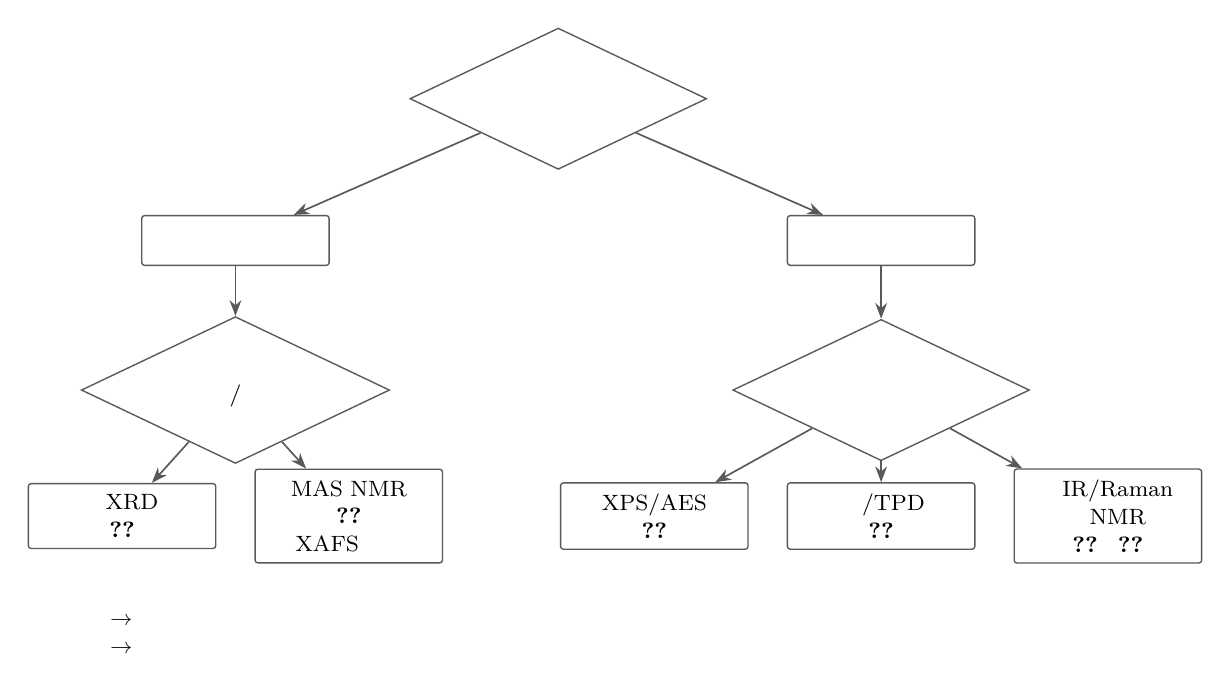
\begin{tikzpicture}[
  x=1mm,y=1mm,
  box/.style={draw=accent,line width=0.5pt,rounded corners=1pt,align=center,
              inner sep=1.4mm,font=\fontsize{8}{10}\selectfont,text width=21mm},
  dec/.style={draw=accent,line width=0.5pt,align=center,inner sep=1.5mm,
              font=\fontsize{8}{10}\selectfont,text width=21mm,
              shape=diamond,aspect=2.1},
  ans/.style={align=center,font=\fontsize{8}{10}\selectfont,text width=21mm},
  ar/.style={-{Stealth[length=2mm]},line width=0.6pt,draw=accent}
]
% 【重叠修正·第二轮】原来各子节点用 below left/right=<v> and <h> of <父> 定位——
% 那定位的是**节点角点**，同一父节点的多个子节点会从父节点中心向两侧铺开而互相侵入。
% 实测 p.6 有 4 对框重叠，最严重一对 66.9x28.4 pt（几乎完全重合）。
% 现在全部改用**显式 (x,y) 坐标**：相邻框中心间距 28.8 mm
% = 框宽 23.8 mm（text width 21 + 2x1.4 内边距）+ 5 mm 缝，是算出来的确定值。
% 图幅 x 从 -67.3 到 81.7 mm = 149 mm，小于单栏版心 165 mm。
\node[dec] (q1) at (0,0) {要问的是\\体相还是表面？};
\node[box] (bulk) at (-41,-18) {体相结构\\晶相、晶胞、价态};
\node[box] (surf) at (41,-18) {表面与界面\\组成、位点、吸附态};
\node[dec] (q2) at (-41,-37) {有序还是\\无定形/短程？};
\node[dec] (q3) at (41,-37) {元素、位点\\还是吸附态？};
\node[box] (xrd) at (-55.4,-53) {多晶 XRD\\\chapref{ch:04}};
\node[box] (nmr) at (-26.6,-53) {MAS NMR\\\chapref{ch:08}\\XAFS（未系统介绍）};
\node[box] (xps) at (12.2,-53) {XPS/AES\\\chapref{ch:09}};
\node[box] (ads) at (41,-53) {化学吸附/TPD\\\chapref{ch:05}};
\node[box] (insitu) at (69.8,-53) {原位 IR/Raman\\原位 NMR\\\chapref{ch:07}\chapref{ch:06}};

\draw[ar] (q1) -- (bulk);
\draw[ar] (q1) -- (surf);
\draw[ar] (bulk) -- (q2);
\draw[ar] (q2) -- (xrd);
\draw[ar] (q2) -- (nmr);
\draw[ar] (surf) -- (q3);
\draw[ar] (q3) -- (xps);
\draw[ar] (q3) -- (ads);
\draw[ar] (q3) -- (insitu);

\node[ans] at (-55.4,-68) {峰位$\to$物相\\峰宽$\to$尺寸};
\node[ans] at (-26.6,-68) {配位\\短程有序};
\node[ans] at (12.2,-68) {元素\\化学态};
\node[ans] at (41,-68) {位点数量\\强度};
\node[ans] at (69.8,-68) {中间物\\反应路径};
\end{tikzpicture}
\caption{方法选择路径。读者应看的是\textbf{分叉的依据}：先分体相/表面，再分「有序程度」或
「要元素、位点还是吸附态」。图中只给最常用的入口，边界情况见正文各章的「互补与回查」
与表~\ref{tab:selector}。\schemamark}
\label{fig:chooseroute}
\end{figure}

\subsection{术语、符号与来源约定}

\begin{itemize}
\item \textbf{缩写}：首次出现给出中文名、英文全称与缩写，后文统一用缩写，保留英文检索入口。
完整缩写表见书末「符号与缩写」。
\item \textbf{符号}：同一符号在不同章可能含义不同（例如 $C$ 在吸附章是 BET 常数、
在动力学章可能指浓度），各章在局部重新定义，不跨章沿用。
\item \textbf{来源标记}：正文用 8\,pt 的方括号短标，形如
\src{S1 §1.1.2，书内 p.17 / PDF p.36，式(1-13)}。
其中 \textbf{S1 = 上册}，\textbf{S2 = 下册}；同时给出书内页码与 PDF 页序，
因为全书页码映射分段，不能套用固定偏移。
\item \textbf{内容性质}：凡不是原书实验结果的数值，一律标 \pedset{教学设定}；
凡原书之外的后续发展，标 \supp{补充} 并给独立来源与日期；
凡尚未对照原页面图像核对的公式，标 \tocheck{待核对}。
\item \textbf{核对状态}：来源标记只说明内容出自原书的哪一处，供回查；本版不标「已核对」。
图与表若有改编、增删列，或含本改编本自己设定的数值，一律在题注内写明。
\item \textbf{图源四类}分别标注：原书实测图（注明册别、书内页码、PDF 页序、原图号）、
\redrawmark（据原书改绘）、\modelmark（模型计算）、\schemamark（示意）。
\end{itemize}

\begin{pitfall}
不要用本书的「来源标记」当作二次文献引用。本书的来源指向原书章节与页码，
用于回查；若你要在论文中引用原始工作，请循原书参考文献找到原始文献并自行核对。
本书不做转引背书。
\end{pitfall}

\subsection{三条阅读路线}

\begin{description}[leftmargin=0pt,style=nextline,font=\heiti]
\item[快速查阅] 用表~\ref{tab:selector} 定位方法，读该章「问题与输出」「误判与边界」两节。
\item[系统学习] 按章顺序读；跨章重复的原理只在主定义处展开，其余以提醒与交叉引用带过。
\item[方案设计] 先读本篇与第 10 章（动力学）确立「要测什么量」，
再按测得量的物理性质选择表征手段，最后用「互补与回查」搭出证据链。
\end{description}
}{}
\setcounter{secnumdepth}{3}

\IfFileExists{chapters/ch01.tex}{% chapters/ch01.tex —— 第 1 章 物理吸附和催化剂的宏观物性测定
% 装配层：只负责按顺序引入各分片。分片缺失时跳过，便于增量成书。
% 分片文件：chapters/parts/ch01-{a..e}.tex

\IfFileExists{chapters/parts/ch01-a.tex}{% ================================================================
%  chapters/ch01.tex
%  第 1 章  物理吸附和催化剂的宏观物性测定
%  源：S1（上册）第 1 章，书内 p.1—84 / PDF p.20—103
%  状态：样章定标部分（1.1—1.2.1），其余节次待续写
% ================================================================

\chapterstart{物理吸附和催化剂的宏观物性测定}%
{本章回答：物理吸附实际测量什么、BET 面积在什么条件下才有物理意义、如何从一条等温线
读出孔结构信息，以及哪些结论不能只靠吸附数据支撑。全章覆盖比表面积、孔容与孔尺寸分布、
颗粒度、密度与机械强度五类宏观物性，其中吸附模型是共用基础，后四类通过速查表调用。}
\label{ch:01}

\subsection{这个方法测量什么}

\begin{probout}
物理吸附测量的是\textbf{气体分子在固体表面的可逆富集量随压力的变化}。得到的原始数据
只有一条曲线：恒温下的吸附量 $V$ 对相对压力 $\ppzero$ 的关系，即吸附等温线
（adsorption isotherm）。由此可以换算三类信息：\textbf{可触及表面积}、\textbf{孔容}
与\textbf{孔尺寸分布}。它不直接给出表面化学状态，也不区分吸附位的种类——同一条等温线
可以由不同的孔结构组合拟合出来。
\end{probout}

物理吸附与化学吸附的差别决定了各自能回答的问题（表~\ref{tab:physis-chemis}）。判据中
最可靠的是吸附热与饱和吸附层数；单凭吸附量大小不能区分二者。

\begin{table}[htbp]
\centering
\caption{物理吸附与化学吸附的判据}
\label{tab:physis-chemis}
{\srcsize
\begin{tabularx}{\columnwidth}{@{}lXX@{}}
\toprule
判据 & 物理吸附 & 化学吸附 \\
\midrule
作用力 & 范德华力（无电子转移） & 化学键（有电子共享或转移） \\
吸附热 & 与液化热同量级，通常 $<\qty{40}{kJ.mol^{-1}}$ & 与反应热同量级，约 $\qtyrange{40}{800}{kJ.mol^{-1}}$ \\
选择性 & 低，任何气体在低温下均可发生 & 高，取决于表面与吸附质的化学匹配 \\
层数 & 多层，不受单层限制 & 单层 \\
可逆性 & 通常可逆，脱附容易 & 常不可逆或需活化能脱附 \\
温度区间 & 低于吸附质临界温度 & 可远高于沸点，甚至高于临界温度 \\
催化相关性 & 仅给出几何信息 & 直接关联活性位 \\
\bottomrule
\end{tabularx}}
\end{table}

\begin{pitfall}
「吸附量很大」不是化学吸附的证据。微孔材料在 $\qty{77}{K}$ 下的氮吸附量可以远超其表面
单层容量，那是\textbf{微孔填充}而非表面吸附；反过来，超临界温度下的物理吸附量可能很小，
却仍然是物理吸附。
\end{pitfall}

\subsection{吸附等温线：唯一的核心数据}

等温线在恒定温度下测定，横轴为相对压力 $\ppzero$（$p_0$ 为该温度下吸附质的饱和蒸气压）。
相对压力而非绝对压力是关键自变量，因为它同时编码了吸附质与吸附剂的相互作用强度。
International Union of Pure and Applied Chemistry（国际纯粹与应用化学联合会，IUPAC）
将物理吸附等温线分为六型（图~\ref{fig:iupac}），分型的依据是\textbf{低相对压力段是否
有拐点}、\textbf{中段是否陡升}和\textbf{高相对压力段是否出现平台}。

\begin{figure}[tbp]
\centering
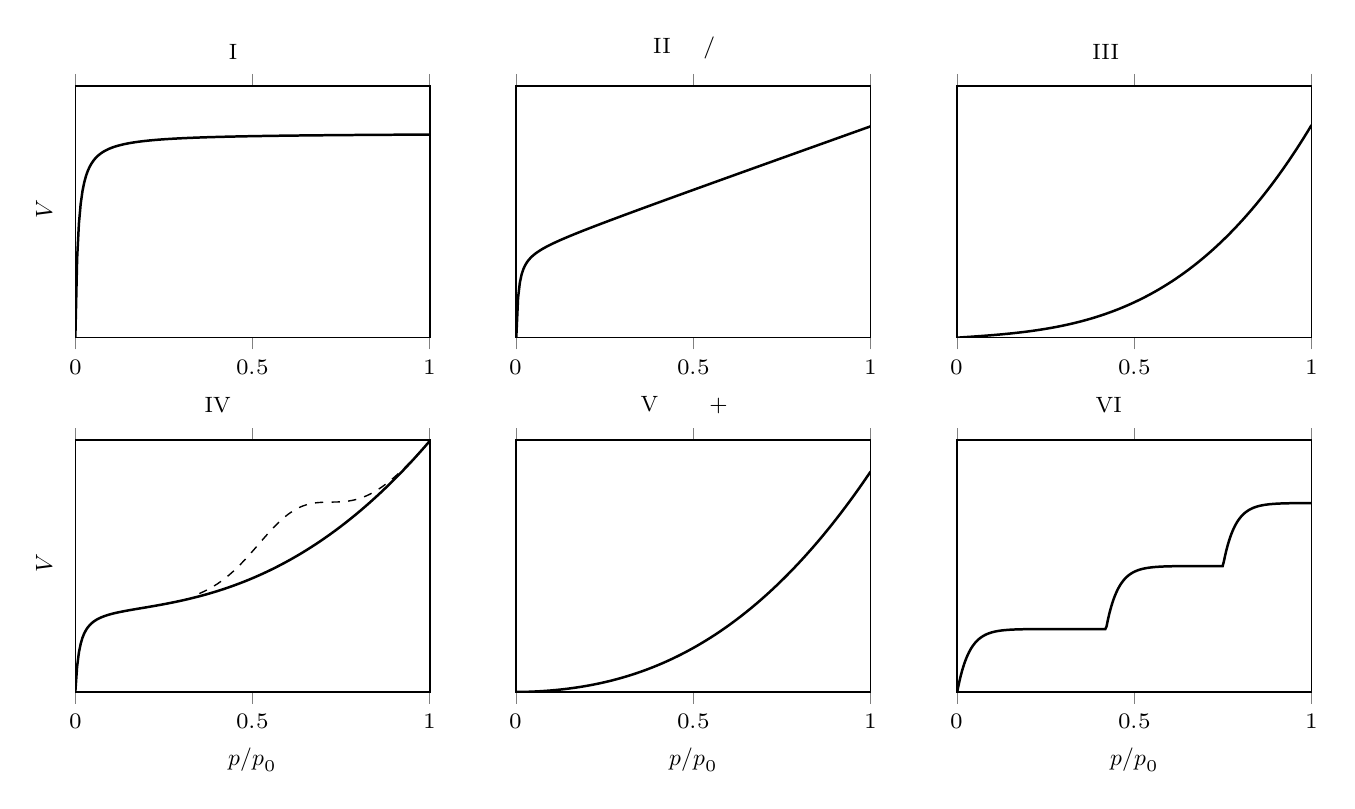
\begin{tikzpicture}
\begin{groupplot}[
  % 单栏改版后版心 165 mm：3×45 + 2×11 = 157 mm，再加左侧轴标签约 3.5 mm 仍有余量。
  % 原为 3×50 + 2×9 = 168 mm，已超出新版权心。
  % vertical sep 由 9 mm 加到 13 mm：原来上排的 x 刻度标签会压到下排的面板标题上
  % （实测 p.7 出现「0.5」与「中孔，带回滞环」等标题文字重叠）。
  group style={group size=3 by 2, xlabels at=edge bottom, ylabels at=edge left,
               horizontal sep=11mm, vertical sep=13mm},
  width=45mm, height=32mm,
  xmin=0, xmax=1, ymin=0, ymax=1.6,
  xtick={0,0.5,1}, ytick=\empty,
  xlabel={$\ppzero$}, ylabel={$V$},
  tick label style={font=\fontsize{8}{9.5}\selectfont},
  scale only axis
]
\nextgroupplot[title={\fontsize{8}{9.5}\selectfont I 型（微孔）}]
\addplot[domain=0:1,samples=200,mainline,black]{1.30*x/(0.008+x)};
\nextgroupplot[title={\fontsize{8}{9.5}\selectfont II 型（非孔/大孔）}]
\addplot[domain=0:1,samples=200,mainline,black]{(x/(0.006+x))*(0.55+0.80*x)};
\nextgroupplot[title={\fontsize{8}{9.5}\selectfont III 型（弱相互作用）}]
\addplot[domain=0:1,samples=200,mainline,black]{0.15*x+1.20*x^3};
\nextgroupplot[title={\fontsize{8}{9.5}\selectfont IV 型（中孔，带回滞环）}]
\addplot[domain=0:1,samples=200,mainline,black]{0.55*x/(0.012+x)+1.05*x^2.5};
\addplot[domain=0.35:1,samples=200,thinline,black,dashed]{0.55*x/(0.012+x)+1.05*x^2.5+0.30*exp(-((x-0.62)/0.16)^2)};
\nextgroupplot[title={\fontsize{8}{9.5}\selectfont V 型（弱相互作用+中孔）}]
\addplot[domain=0:1,samples=200,mainline,black]{0.30*x^1.6+1.10*x^2.6};
\nextgroupplot[title={\fontsize{8}{9.5}\selectfont VI 型（逐层吸附）}]
\addplot[domain=0:1,samples=300,mainline,black]{0.40*(1-exp(-30*x))+0.40*(1-exp(-30*max(x-0.42,0)))+0.40*(1-exp(-30*max(x-0.75,0)))};
\end{groupplot}
\end{tikzpicture}
\caption{IUPAC 六型物理吸附等温线。读者应看三处：低相对压力段有无拐点、中段是否陡升、
高相对压力段有无平台。实线为吸附支，虚线为脱附支。本图为按各型特征函数计算的示意曲线，
不代表任何具体样品。\schemamark\figsrc{据 S1（上册）图 1-7，书内 p.19 / PDF p.38 改绘。}}
\label{fig:iupac}
\end{figure}

六型等温线可读出的信息归纳于表~\ref{tab:isotherm-read}。注意\textbf{分型是定性判断，
不是定量结论}：实际样品常是混合孔结构，等温线介于两型之间。

\begin{table}[htbp]
\centering
\caption{由等温线类型可读出的信息与常见误判}
\label{tab:isotherm-read}
{\srcsize
\begin{tabularx}{\columnwidth}{@{}lXX@{}}
\toprule
类型 & 可读出 & 易误判之处 \\
\midrule
I & 微孔为主；平台值即微孔孔容 & 用 BET 计算「表面积」，实为等效值；用 BJH 分析会得到虚假孔径 \\
II & 非孔或大孔；拐点 B 对应单层铺满 & 把拐点吸附量直接当 $V_{\mathrm{m}}$（仅在 $C\approx9$ 时成立） \\
III & 吸附质--吸附剂相互作用弱 & 误判为「无孔」；实为相互作用弱，宜换吸附质 \\
IV & 中孔；中段陡升为毛细凝聚 & 忽略回滞环就丢掉孔尺寸信息 \\
V & 弱相互作用 + 中孔 & 同 III 型，先换吸附质再谈孔结构 \\
VI & 逐层吸附，表面高度均一 & 少见；出现时应先怀疑测量或样品异常 \\
\bottomrule
\end{tabularx}}
\end{table}

\subsection{核心公式及其成立条件}

\subsubsection{Langmuir 等温式}

Langmuir 模型假设：表面吸附位等价且互不影响、吸附为单层、吸附与脱附达到动态平衡。
由吸附速率与脱附速率相等可得

\begin{equation}\label{eq:langmuir}
\theta=\frac{V}{V_{\mathrm{m}}}=\frac{b\,p}{1+b\,p}
\end{equation}

其中 $V$ 为吸附量，$V_{\mathrm{m}}$ 为单层饱和吸附量，$b$ 为吸附平衡常数，$p$ 为平衡压力。
重排为直线形式后可由斜率与截距求两个参数：

\begin{equation}\label{eq:langmuir-lin}
\frac{p}{V}=\frac{1}{V_{\mathrm{m}}b}+\frac{p}{V_{\mathrm{m}}}
\end{equation}

\begin{keycond}
式~\eqref{eq:langmuir} 仅在\textbf{能量均匀、无相互作用、单层}的前提下成立。真实氧化物表面
存在多种羟基与配位不饱和位，能量并不均匀。实践中的经验是：当覆盖度落在
$\theta\approx\qtyrange{0.1}{0.4}{}$ 的中等区间时，表面不均匀性与吸附质侧向相互作用的
影响部分抵消，$b$ 近似为常数，此时物理吸附等温线可用 Langmuir 公式近似表征
\src{S1 §1.1.2，书内 p.16--17 / PDF p.35--36}。超出该区间，参数会随拟合窗口漂移。
\end{keycond}

\subsubsection{BET 等温式与比表面积}

BET 模型保留 Langmuir 的「吸附位等价、分子间无相互作用」假设，补充两条：吸附可以是
多分子层的，且不必铺满单层后再铺下一层；第一层的吸附热 $E_1$ 与固体表面直接作用有关，
第二层以后各层吸附热相同，等于吸附质的液化热 $E_{\mathrm{L}}$。据此得到的二常数公式为

\begin{equation}\label{eq:bet}
V=\frac{V_{\mathrm{m}}C\,\ppzero}{\left(1-\ppzero\right)\left[1+(C-1)\ppzero\right]}
\end{equation}

其中 $C$ 为与 $E_1$、$E_{\mathrm{L}}$ 及温度有关的常数，反映吸附质与吸附剂相互作用的强弱，
并可近似写作

\begin{equation}\label{eq:cdef}
C\approx\exp\!\left[\frac{E_1-E_{\mathrm{L}}}{RT}\right]
\end{equation}

式~\eqref{eq:bet} 的直线形式是实际计算的依据：

\begin{equation}\label{eq:bet-lin}
\frac{\ppzero}{V\left(1-\ppzero\right)}
=\frac{C-1}{V_{\mathrm{m}}C}\cdot\ppzero+\frac{1}{V_{\mathrm{m}}C}
\end{equation}

以 $\ppzero$ 为横轴、$\ppzero/[V(1-\ppzero)]$ 为纵轴作图，斜率 $=(C-1)/(V_{\mathrm{m}}C)$，
截距 $=1/(V_{\mathrm{m}}C)$，由此解得 $V_{\mathrm{m}}$ 与 $C$。总表面积由单层容量换算：

\begin{equation}\label{eq:surface}
S=\frac{V_{\mathrm{m}}\,N_{\mathrm{A}}\,\sigma}{22400}
\end{equation}

式中 $S$ 为吸附剂总表面积，$\sigma$ 为吸附质分子的截面积，$N_{\mathrm{A}}$ 为阿伏伽德罗常量，
分母 $22400$ 为标准状况下气体的摩尔体积（$\unit{mL.mol^{-1}}$）；比表面积即 $S$ 除以样品质量。
式~\eqref{eq:surface} 的量纲检查：$V_{\mathrm{m}}$ 取 $\unit{mL.g^{-1}}$ 时，
$\unit{mL.g^{-1}}\times\unit{mol^{-1}}\times\unit{m^2}$ 除以 $\unit{mL.mol^{-1}}$ 得
$\unit{m^2.g^{-1}}$，与比表面积单位一致。

\begin{keycond}
二常数 BET 公式\textbf{只在 $\ppzero\approx\qtyrange{0.05}{0.35}{}$ 区间成立}，更可靠的
窗口是 $\qtyrange{0.05}{0.30}{}$。原因有两条：低于 $0.05$ 时多层吸附尚未建立，表面不均匀性
凸显；高于 $0.35$ 时毛细凝聚破坏了多层吸附模型 \src{S1 §1.1.2，书内 p.18 / PDF p.37}。
对吸附能较高的体系，线性范围会向低相对压力移动，因此\textbf{不可照搬固定窗口}，
应以残差图和线性度判断。为保证可靠性，作图至少使用五个数据点。
\end{keycond}

\begin{figure}[htbp]
\centering
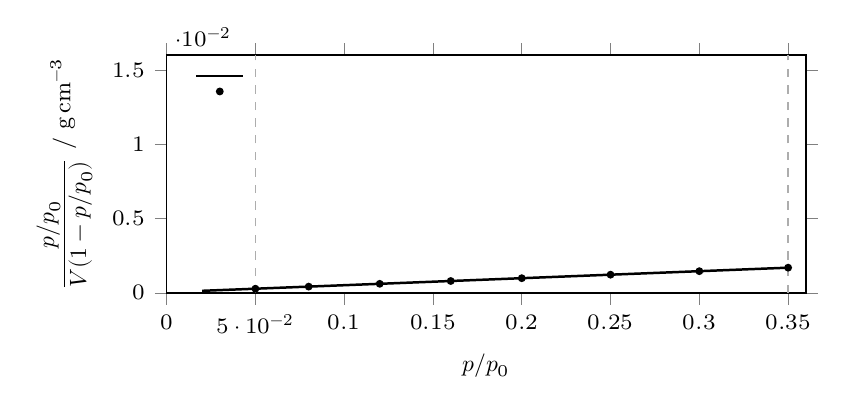
\begin{tikzpicture}
\begin{axis}[
  width=\onecolwidth, height=46mm,
  xlabel={$\ppzero$}, ylabel={$\dfrac{\ppzero}{V(1-\ppzero)}$ / $\unit{g.cm^{-3}}$},
  xmin=0, xmax=0.36, ymin=0, ymax=0.016,
  legend pos=north west, legend cell align=left]
% 教学设定：Vm = 210 cm3/g, C = 120  -> 斜率 4.72e-3, 截距 3.97e-5
\addplot[domain=0.02:0.35,samples=2,mainline,black]{4.72e-3*x+3.97e-5};
\addplot[only marks,mark=*,mark size=1.1pt,black] coordinates{
 (0.050,0.000276)(0.080,0.000417)(0.120,0.000606)(0.160,0.000795)
 (0.200,0.000984)(0.250,0.001220)(0.300,0.001456)(0.350,0.001692)};
\legend{回归直线,数据点（教学设定）}
% 0.05–0.35 适用窗口
\draw[accentsoft,dashed,thinline] (axis cs:0.05,0) -- (axis cs:0.05,0.016);
\draw[accentsoft,dashed,thinline] (axis cs:0.35,0) -- (axis cs:0.35,0.016);
\node[anchor=north east,font=\fontsize{8}{9.5}\selectfont,color=accent]
  at (axis cs:0.345,0.0158) {适用窗口};
\end{axis}
\end{tikzpicture}
\caption{BET 直线形式。读者应看三处：数据点是否落在 $0.05$--$0.35$ 窗口内、
是否成直线、截距是否为正。截距为负说明 $C<0$，此时由式~\eqref{eq:surface} 得到的
「表面积」没有物理意义，应改用别的模型或更换吸附质。
数据点为\textbf{教学设定}的合成值（$V_{\mathrm{m}}=\qty{210}{cm^3.g^{-1}}$，$C=120$），
不是实验数据。\modelmark\figsrc{式~\eqref{eq:bet-lin} 据 S1（上册）式(1-15)，书内 p.18 / PDF p.37。}}
\label{fig:betplot}
\end{figure}

\subsection{数据到结论：比表面积的求算流程}

\begin{dataflow}
（1）确认等温线类型。I 型或含显著微孔者，BET 结果只能称为\textbf{等效 BET 表面积}
（equivalent BET surface area），不可当作真实表面积极使用。（2）选取 $\ppzero$ 窗口，
优先 $\qtyrange{0.05}{0.30}{}$，并用至少五个点。（3）按式~\eqref{eq:bet-lin} 线性回归，
\textbf{必须检查截距为正}。（4）由斜率和截距解 $V_{\mathrm{m}}$ 与 $C$，按
式~\eqref{eq:surface} 换算比表面积。（5）报告时同时给出取样窗口、数据点数与 $C$ 值——
缺少这三项的表面积数值无法复核。
\end{dataflow}

对已知表面性质的大孔或非孔样品，当 $C>50$ 时可用\textbf{单点 BET 法}：取窗口内一个点，
以 $V_{\mathrm{m}}=V(1-\ppzero)$ 求算，与多点法的偏差通常小于 $5\%$，适合快速筛选
\src{S1 §1.2.1，书内 p.42 / PDF p.61}。$C$ 值未知时不应使用单点法。

\subsection{误判与边界}

\begin{pitfall}
\textbf{（1）微孔材料的 BET 面积被系统性高估。}低相对压力下（$\ppzero<0.1$）微孔填充的
吸附量无法从单层吸附量中扣除，所得值为等效值 \src{S1 §1.2.1，书内 p.42 / PDF p.61}。
\textbf{（2）含 $2$--$\qty{4}{nm}$ 中孔时单层吸附量被高估。}单层铺满与毛细凝聚开始的相对
压力过于接近，两者在等温线上不可分辨。\textbf{（3）回归相关系数高不等于模型正确。}
$R^2$ 只说明数据在该窗口内近似线性，不说明 BET 假设成立；必须同时检查 $C>0$ 与
$V_{\mathrm{m}}$ 的合理性。\textbf{（4）回滞环不能进入 BET 拟合。}BET 公式不处理毛细凝聚，
拟合应只用吸附支，且避开回滞环所在压力区间。
\end{pitfall}

\begin{crosscheck}
表面积是几何量，不能单独支撑结构结论。判断物相与晶体结构应用多晶 X 射线衍射
（\chapref{ch:04}）；判断表面元素与化学态应用 X 射线光电子能谱（\chapref{ch:09}）；
判断孔尺寸分布应与压汞法在重叠孔径区间相互印证；判断活性位数量需化学吸附与程序升温
技术（\chapref{ch:05}）。若吸附法与压汞法给出的孔容不一致，应先复查样品预处理与
模型假设，而不是取两者平均。
\end{crosscheck}

\srcnote{本节来源：S1（上册）§1.1--§1.2.1，书内 p.1--42 / PDF p.20--61。
式~\eqref{eq:langmuir}--\eqref{eq:surface} 已按原页面图像（PDF p.36--37）逐式核对；
数值算例为教学设定，非原书实验结果。其余节次（孔容与孔尺寸分布、颗粒度、密度、
机械强度）的来源定位见\texttt{sources/coverage.csv}。}
}{}
\IfFileExists{chapters/parts/ch01-b.tex}{% ================================================================
%  chapters/parts/ch01-b.tex  —  第 1 章 分片 b
%  §1.2.2  孔容和孔尺寸分布
%  源：S1（上册）§1.2.2，书内 p.43—60 / PDF p.62—79
%  接 ch01-a.tex（比表面积）之后；颗粒度、密度、机械强度见分片 c
% ================================================================

\subsection{孔容和孔尺寸分布}

\begin{probout}
\textbf{本节回答}：一条已经测好的吸附等温线，如何变成孔容与孔尺寸分布，这些数值在什么
条件下可信，以及为什么不同方法报出的「平均孔径」不能直接互相比较。比表面积的求算流程
见 \chapref{ch:01} 前一节。

\textbf{输出}：比孔容（$\unit{cm^3.g^{-1}}$ 或 $\unit{mL.g^{-1}}$）与孔尺寸分布曲线
——通常画成 $\mathrm{d}V_p/\mathrm{d}\lg D_p$ 对 $\lg D_p$，以及由分布派生的总孔容、
最可几孔宽和外表面积。

\textbf{本节核心判断}：孔尺寸分布\textbf{不是被「测」出来的，而是用一个模型从等温线
反演出来的}。原始数据只有一条曲线；要把它变成分布，必须补上三重假定：（i）孔的形状是
圆柱形、平板狭缝还是球形；（ii）吸附层厚度 $t$ 与相对压力、与孔壁曲率的关系；
（iii）孔之间互不连通、互不干扰。这三条都写在模型里，不在数据里。于是\textbf{换模型就
换分布}：同一组数据用 BJH 与 NLDFT 反演，峰的位置、个数和高度都可以不同
（图~\ref{fig:psd-model}）。因此报告孔尺寸分布时\textbf{必须同时给出实验方法、吸附质和
模型（含 kernel）名称}三项，缺任何一项，数值都无法复核，也无法与文献比较。
\end{probout}

\subsubsection{孔、孔宽与等效孔模型}

按与外界是否连通，孔分为\textbf{开孔}（open pore，与外界连通的孔）、\textbf{盲孔}
（blind pore，只有一个外界连通开口的开孔）与\textbf{闭孔}（closed pore，不与外界连通的
孔）。只有反应物、产物分子能进出的开孔对催化有意义；闭孔不参与吸附与扩散，气体吸附法
测不到它，需用小角 X 射线散射或小角中子散射，本节不涉及。

孔尺寸用\textbf{孔宽}（pore width）标示：圆柱形孔取孔直径而非半径，平板孔取板壁间距，
二者统称孔宽。作这一约定是为了让两种等效孔模型的数值对吸附质的容纳能力具有可比性；本书
一律用「孔尺寸」而非「孔径」，因为实际的孔极少是圆的。

真实催化剂内部的孔极不规则，无法用纯几何特征值描述。间接测定法所做的，是把真实孔系统
\textbf{等效为一组尺寸不同、形状规整、互不连通的模型孔}，使流体在这组模型孔上的渗透与
滞留行为与真实样品相同。由此得到的分布是\textbf{等效模型孔的理想分布，只是名义值}，
具有平均或等效的意义，不再反映真实孔的实际几何；它\textbf{完全依赖于测定方法（流体
分子的性质）和分析理论（所采用的孔模型）}。虽然失去了确定的几何意义，这一结果对理解
催化剂的吸附能力与催化活性恰恰十分有用。还须注意，现有孔分析理论都假定\textbf{各孔互不
连通、相互独立}，而真实催化剂是多孔网络，「墨水瓶」孔、并行喉管、连通腔体都超出模型的
表达能力；孔之间的连通性目前只能用回滞环扫描等手段定性了解
\src{S1 §1.2.2，书内 p.43--45 / PDF p.62--64}。

\subsubsection{毛细凝聚与 Kelvin 方程}

\begin{principle}
\textbf{物理图像}：中孔内先由吸附质以液膜形式覆盖孔壁，液膜厚度 $t$ 随 $\ppzero$ 增大而
增厚；当液膜围成的「孔心」达到弯曲液面的平衡条件时，孔心发生\textbf{毛细凝聚}
（capillary condensation），孔被凝聚液充满。描述这一平衡的是 Kelvin 方程：

\begin{equation}\label{eq:kelvin}
\ln\frac{p}{p_0}=-\frac{2\gamma V_{\mathrm{L}}\cos\theta}{r_kRT}
\end{equation}

式中 $\gamma$ 为液体的表面张力，$V_{\mathrm{L}}$ 为液体的摩尔体积，$\theta$ 为液体与孔壁
的接触角（氮在 $77\,\unit{K}$ 下润湿孔壁，$\cos\theta\approx1$），$R$ 为摩尔气体常量，
$T$ 为热力学温度，$r_k$ 为\textbf{弯月面的曲率半径}，称 Kelvin 半径。

量纲检查：$\gamma V_{\mathrm{L}}$ 为 $\unit{N.m^{-1}}\times\unit{m^3.mol^{-1}}
=\unit{N.m^2.mol^{-1}}$，除以 $r_k$（$\unit{m}$）得 $\unit{N.m.mol^{-1}}$，与
$RT$（$\unit{J.mol^{-1}}=\unit{N.m.mol^{-1}}$）之比无量纲，与等式左边的对数一致。

\textbf{$r_k$ 不是孔半径}：它只是发生凝聚的孔心半径，而孔壁上已存在厚度为 $t$ 的吸附层，
故真实孔半径 $r_p=r_k+t$。这一步称\textbf{曲率修正}；不做修正而直接以 $r_k$ 当孔半径，
会把孔算小，并把表面积算大。
\end{principle}

\begin{keycond}
\textbf{（1）弯月面形状决定系数。}式~\eqref{eq:kelvin} 中的系数 $2$ 对应\textbf{半球形}
弯月面；对圆柱形弯月面，平均曲率减半，系数应改为 $1$。脱附时凝聚液自孔口以半球形弯月面
蒸发，吸附时孔内凹液面为圆柱面，二者给出不同的 $r_k$--$\ppzero$ 关系——这正是回滞环的
几何来源。使用前必须先确认所用公式对应吸附支还是脱附支。
\textbf{（2）只在中孔内成立。}微孔的孔径与吸附质分子尺寸同量级，孔壁势场叠加，流体不再
具有体相性质，连续介质图像失效。
\textbf{（3）数值常数与吸附质、温度绑定。}以 $77\,\unit{K}$ 氮吸附为例，取
$\gamma=\qty{8.85}{mN.m^{-1}}$、$V_{\mathrm{L}}=\qty{34.7}{cm^3.mol^{-1}}$、
$\cos\theta=1$，则 $2\gamma V_{\mathrm{L}}/(RT)=\qty{0.955}{nm}$，即
$r_k/\unit{nm}=0.955\big/\ln(p_0/p)$；代入 $\ppzero=0.5$ 得 $r_k\approx\qty{1.38}{nm}$，
同点 $t\approx\qty{0.68}{nm}$，故 $r_p\approx\qty{2.06}{nm}$、$D_p\approx\qty{4.1}{nm}$。
该算例用于校核常数取值，不是实验值。\tocheck{未对照原页面图像：原书在 Kelvin 公式处给出的
常数取值与量纲约定（$r_k$ 以 nm 或 Å、是否已含 $\cos\theta$）OCR 未保留，上列常数系按
标准物理量自行计算。}
\end{keycond}

\subsubsection{BJH 法：中孔分布的记账框架}

BJH 法（Barrett--Joyner--Halenda 法）采用\textbf{圆柱形盲孔等效模型}，假定孔之间互不
连通、各孔在吸附或脱附过程中彼此独立，并假定中孔内液膜厚度 $t$ \textbf{只与相对压力
有关}，与吸附质性质和孔半径无关。其核心是一步守恒记账：相对压力 $x_k=(p/p_0)_k$ 下的
总吸附量等于\textbf{已凝聚孔内的液量}与\textbf{未凝聚孔壁上的液膜量}之和。

\begin{equation}\label{eq:bjh-balance}
V(x_k)=\underbrace{\sum_{i\le k}\pi r_i^{2}\ell_i}
_{\text{半径 }r_i\le r_k\text{ 的孔：已充满，计全孔体积}}
\;+\;\underbrace{\sum_{j>k}\pi\!\left[r_j^{2}-\left(r_j-t_k\right)^{2}\right]\ell_j}
_{\text{尚未凝聚的孔：只计孔壁液膜体积}}
\end{equation}

式中 $r_i$、$\ell_i$ 为第 $i$ 组孔的半径与该组孔总长度，$r_k$ 为 $x_k$ 对应的 Kelvin
半径，$t_k=t(x_k)$ 为对应液膜厚度，且孔半径与膜厚满足 $r_i=r_k(x_i)+t(x_i)$——孔壁上先有
厚度 $t$ 的吸附层，余下的孔心半径才是 Kelvin 半径（见本节前文曲率修正）。
\textbf{两项记的是两件不同的事，不能互相套用公式}：
\textbf{（1）已凝聚的孔}（$r_i\le r_k$）内是\textbf{充满}的液体，单位孔长的液量就是全孔
截面积 $\pi r_i^{2}$，即整个体积 $\Delta V_i=\pi r_i^{2}\ell_i$；
\textbf{（2）尚未凝聚的孔}（$r_j>r_k$）只有孔壁上的液膜，单位孔长液量为全截面积减去
未填的孔心 $\pi[r_j^{2}-(r_j-t_k)^{2}]$，即等价的环形面积。若把第 (1) 项误写成
$\pi[r_i^{2}-(r_i-t_k)^{2}]$，等于把已充满的孔当成只剩一圈液膜的孔：取 $r_i=\qty{5}{nm}$、
$t_k=\qty{1}{nm}$，正确的单位孔长液量是 $25\pi\,\unit{nm^2}$，误式只给 $9\pi\,\unit{nm^2}$
（少 $64\%$）；更荒谬的是令 $t_k\to0$ 时误式给出\textbf{零体积}，而充满的孔
体积与膜厚无关。

\textbf{液膜项的薄膜近似}：环面积可展开为
$r_j^{2}-(r_j-t_k)^{2}=2r_jt_k-t_k^{2}$，当 $t_k\ll r_j$ 时略去 $t_k^{2}$ 得
$2r_jt_k$（$t_k/r_j=0.04$ 时高估 $2\%$）。本书保留精确的环形写法，只有在孔半径远大于
膜厚、且明确注明薄膜近似时才用 $2\pi r_j\ell_jt_k$。

式~\eqref{eq:bjh-balance} 各项都是体积，故可直接相加；
相邻两个相对压力下的差值 $V(x_{k+1})-V(x_k)$ 给出 $r_k$ 至 $r_{k+1}$ 区间的孔容增量，
累加得积分分布，求导得微分分布 $\mathrm{d}V_p/\mathrm{d}D_p$，其最高峰对应
\textbf{最可几孔宽}。

\textbf{递推的物理含义}：相对压力升高时，孔壁液膜继续增厚，毛细凝聚同时向更大的孔推进，
两个过程都在消耗吸附量，必须逐级扣除，不能把吸附量增量全部记到新凝聚的那组孔上——这
正是 BJH 手工推算冗长繁琐的原因。石油化工行业标准 SH/T 0572—1993《孔尺寸分布计算法
（氮脱附等温线计算法）》给出这套递推的具体算法，商品吸附仪均内置相应程序；孔宽与相对
压力的对应关系即

\begin{equation}\label{eq:bjh-dp}
D_p=2\left(r_k+t\right),\qquad \ppzero=0.95\;\Longleftrightarrow\;D_p\approx\qty{50}{nm}
\end{equation}

\tocheck{未对照原页面图像：原书式(1-36)的符号体系（$V(x_k)$、$r_i$、$t_k$ 的下标约定与
求和上下限）OCR 完全失真，式~\eqref{eq:bjh-balance} 按 BJH 原始记账方式重写。其中
\textbf{第 (1) 项「已充满孔计全孔体积 $\pi r_i^{2}\ell_i$」不是从 OCR 判读出来的，而是由
该式自身的物理含义推定的}——已凝聚的孔内是充满的液体，写成环形面积
$\pi[r_i^{2}-(r_i-t_k)^{2}]$ 会让「充满的孔」在 $t_k\to0$ 时体积归零，与该式的定义自相
矛盾（本节已就该式加数值自检）。原书该项的确切写法仍需查 PDF p.65 原页面核对；
SH/T 0572 的标准年份与完整题名亦未在图像上确认。}

\begin{keycond}
\textbf{BJH 的三个硬边界。}（1）\textbf{不适用于微孔}：$\ppzero<0.2$ 的吸附量变化由微孔
填充贡献，Kelvin 方程在此无物理意义，强行计算会得到虚假峰。（2）\textbf{孔宽有上下限}：
由式~\eqref{eq:bjh-dp}，$77\,\unit{K}$ 氮吸附下 BJH 计算中孔孔宽的\textbf{上限约
$\qty{50}{nm}$}，用脱附支计算时可靠\textbf{下限为 $\qtyrange{5}{6}{nm}$}；两端之外应改用
压汞法（大孔端）或微孔方法（小孔端）。（3）\textbf{孔宽小于临界宽度 $D_{\mathrm{ch}}$ 时
没有回滞环}：此时等温线为完全可逆的 IV(b) 型，但仍可由毛细凝聚造成台阶。孔宽约
$\qty{4}{nm}$ 的 MCM-41 在 $77\,\unit{K}$ 氮吸附下即为无回滞环的 IV(b) 型，台阶跃升位于
$\ppzero=0.41$--$0.46$，由柱状孔几何算得的平均孔宽 $\qty{3.2}{nm}$ 仍真实反映了该材料；
换用 $77\,\unit{K}$ 氧吸附后等温线变为 IV(a) 型，回滞环出现在 $\ppzero=0.34$--$0.44$，
估算孔宽 $\qtyrange{3.0}{3.2}{nm}$。\textbf{无回滞环不等于无中孔}
\src{S1 §1.2.2 1)，书内 p.45--48 / PDF p.64--67}。
\end{keycond}

BJH 假定孔内液膜的化学势等于液体本体的化学势，但这样的液膜在热力学上是不稳定的。
Broekhoff 与 de Boer 考虑了两者化学势的差别，指出液膜厚度不仅与相对压力有关，还与液膜
曲率（即孔半径）有关，据此给出满足热力学平衡条件的 \textbf{BdB 法}；当回滞环明显、孔壁
曲率影响不可忽略时，BdB 法比 BJH 法更自洽，代价是计算量更大。

\subsubsection{$t$ 图法与微孔分析：MP 法}

\begin{principle}
\textbf{前提}：非孔性固体上，当表面吸附多于单层后，氮的吸附层数 $n$（或厚度 $t$）
\textbf{只与相对压力有关，而与吸附剂种类无关}，因此对一种吸附质存在一条\textbf{通用标准
吸附等温线}（$t$ 曲线）。这是全部 $t$ 类方法的共同基石，它的失效方式也决定了这些方法的
误差来源。吸附层厚度与相对压力的经验关系（Halsey 方程）为

\begin{equation}\label{eq:halsey}
t=t_{\mathrm{m}}\left[\frac{-5}{\ln\left(\ppzero\right)}\right]^{1/3}
\end{equation}

$t_{\mathrm{m}}$ 为氮的单分子层平均厚度，取 $\qty{0.354}{nm}$；式~\eqref{eq:halsey}
在 $\ppzero\to1$ 时发散，只能用于毛细凝聚显著之前的区间。
\tocheck{未对照原页面图像：原书式(1-37) 的指数与常数（$-5$、$1/3$）在 OCR 中失真，
此处按 Halsey 方程标准形式重建；$t_{\mathrm{m}}=\qty{0.354}{nm}$ 取自 OCR 正文。}吸附量与厚度成正比：

\begin{equation}\label{eq:vt}
V=\frac{V_{\mathrm{m}}}{t_{\mathrm{m}}}\,t
\end{equation}

即 $V$--$t$ 图在非孔性吸附剂上应是一条\textbf{过原点的直线}，斜率等于
$V_{\mathrm{m}}/t_{\mathrm{m}}$，说明吸附量增加时留存表面积不变。\textbf{若吸附量以
凝聚态液氮体积为单位，则该斜率直接给出比表面积}：斜率单位为
$\unit{cm^3.g^{-1}}/\unit{nm}=10^{7}\,\unit{cm^2.g^{-1}}$，而 $\qty{1}{cm^3}$ 液氮铺成
厚 $\qty{0.354}{nm}$ 的膜时覆盖 $1/0.354\times10^{7}\approx2.8\times10^{7}\,
\unit{cm^2}$，两者一致，故有换算
$S/(\unit{m^2.g^{-1}})\approx10^{3}\times\dfrac{V_{\text{液}}/(\unit{cm^3.g^{-1}})}
{t/(\unit{nm})}$；用标准状况体积表示时等价于 $S\approx1.54\,V_{\mathrm{STP}}/t$。
\tocheck{未对照原页面图像：原书在 $V$--$t$ 斜率处只写「此斜率即为样品的表面积」，未标明
体积单位与 $10^{3}$ 这一换算因子；上列因子按液氮密度自行推导。}
\end{principle}

\textbf{多孔吸附剂的 $V$--$t$ 曲线形状与判读。}与过原点直线相比共有四种典型偏离方式：
\textbf{微孔}存在时，很低的相对压力下即发生微孔填充，被充满的微孔不能再发展多层吸附、
留存表面积下降，曲线\textbf{向下（上凸）偏离}；\textbf{中孔}存在时，中等相对压力下发生
毛细凝聚，吸附量急剧增加而标准 $t$ 值增加很小，曲线\textbf{向上偏离}；\textbf{中孔与微孔
共存}时曲线呈 \textbf{S 形}；毛细凝聚完成后吸附只在外表面继续，曲线\textbf{再次成为
直线}，其\textbf{斜率反映外表面积}、\textbf{截距等于中孔孔容}
\src{S1 §1.2.2 3)a，书内 p.52--53 / PDF p.71--72}。

\begin{keycond}
\textbf{$t$ 方法的两条实用条件。}（1）$V$--$t$ 曲线\textbf{并不总能过原点}，这是吸附质
与吸附剂相互作用强度不同造成的；按化学性质或按相互作用强度分级建立多套标准等温线，正是
对 $t$ 方法的改进方向。（2）用低相对压力段（$\ppzero<0.4$ 附近）的直线斜率求总表面积、
用高相对压力段的直线截距求中孔孔容，是\textbf{两个彼此独立的步骤}，不能用同一段直线同时
得出；进入回滞区后 $t$ 值物理意义消失，两段直线的判读随之失效。
\end{keycond}

\textbf{MP 法（微孔法）}是 $t$ 方法在微孔上的扩展。微孔吸附剂的 $V$--$t$ 曲线必然向下
弯曲偏离直线（反之不成立），下弯段本身即携带微孔孔尺寸信息。取平行板狭缝模型，微孔容
$V$、孔壁面积 $S$ 与厚度 $t$ 满足 $V=S\,t$；在弯曲段某点 $t_i$ 处的\textbf{切线斜率即
该厚度下留存的表面积} $S_i$，厚度增至 $t_{i+1}$ 时更大的微孔被充满，而被充满那组微孔的
板间距正对应 $t_{i+1}$。于是第 $i$ 组微孔的孔容为

\begin{equation}\label{eq:mp-dv}
\Delta V_i=\Delta S_i\,\bar{t}_i,\qquad
\Delta S_i=S_{i-1}-S_i,\qquad
\bar{t}_i=\tfrac12\left(t_i+t_{i+1}\right)
\end{equation}

由 $\Delta V_i$ 对该组孔宽（平板模型取 $D_{p,i}\approx2t_i$）作图即得微孔孔尺寸分布。
量纲检查：$\Delta S_i$ 为 $\unit{m^2.g^{-1}}$、$\bar{t}_i$ 为 $\unit{nm}$，乘积为
$\unit{nm.m^2.g^{-1}}=10^{-7}\,\unit{cm^3.g^{-1}}$，与孔容单位一致。
\tocheck{未对照原页面图像：原书式(1-42)--(1-44) 的下标约定（$\bar t_i$ 取相邻均值还是端点
值）与「板间距 $=t_{i+1}$ 还是 $=2t_i$」在 OCR 中无法判读，此处按 MP 法通用约定重写。}
两个使用要点：其一，低 $t$ 段过原点直线的斜率给出\textbf{总表面积}，大 $t$ 段直线外推的
\textbf{截距给出微孔总孔容}、斜率给出\textbf{外表面积}；该分析\textbf{隐含平板狭缝孔
假设，不适用于圆柱形微孔}，且微孔材料的总表面积本身物理意义有限。其二，MP 法同样按 BET
公式的 $C$ 值划分相互作用强弱并选择相应 $t$ 曲线（同一相对压力下相互作用强的体系液膜
稍厚），也可用与样品化学性质相同的非孔性吸附剂作基准物建立专属标准等温线
\src{S1 §1.2.2 3)c，书内 p.54--56 / PDF p.73--75}。

\subsubsection{标准吸附等温线对比法：$t$、$\alpha_s$ 与 $n$ 曲线}

$t$ 方法、$\alpha_s$ 方法与 $n$ 方法\textbf{都不是从理论模型推导出来的}，而是从大量
实验数据中归纳出的经验方法，同属「标准吸附等温线对比法」。它们的共同操作是：把多孔样品
的吸附量 $V$ 对一个描述吸附层状态的归一化量作图，由直线的斜率与弯曲位置读出表面积与
孔容；判读规则三者通用——过原点直线给出总表面积，下弯表示微孔填充，上弯表示毛细凝聚，
高段直线的斜率与截距给出外表面积与中孔（或微孔）孔容。

\textbf{$\alpha_s$ 方法}不用吸附层厚度，改用归一的吸附量 $a_s$，以非孔性参考吸附剂上
相对压力为 $0.4$ 时的吸附量 $n_{0.4}$ 作分母：

\begin{equation}\label{eq:as}
a_s=\frac{n\!\left(\ppzero\right)}{n_{0.4}}
\end{equation}

对同一类吸附剂建立统一的 $\alpha_s$ 曲线（$\alpha_s$ 对 $\ppzero$ 的标准数据表），再把
多孔样品各相对压力下的 $n$ 对 $a_s$ 作图得 $V$--$\alpha_s$ 图，判读方式与 $V$--$t$ 图
完全平行。\tocheck{未对照原页面图像：原书式(1-39) 的完整形式（分子分母记号，以及横轴是
$\ppzero$ 还是归一化后的 $(p/p_0)/0.4$）OCR 失真。}

\textbf{$n$ 方法}进一步认为吸附层厚度（以层数 $n=V/V_{\mathrm{m}}$ 表示）不仅取决于
相对压力，还取决于吸附质与吸附剂相互作用的强度；由于 BET 公式中的 $C$ 值恰好反映这一
强度，故按 $C$ 值分级（例如 $C>300$、$300>C>100$、$100>C>40$、$40>C>30$ 等）分别建立
$n$ 标准等温线。多孔样品作图时须先按自身 $C$ 值\textbf{选择合适的那一条}曲线；按 $C$ 值
分类的做法，实质是把 $t$ 方法「存在一条与吸附剂无关的标准等温线」的假设放宽为「同一
相互作用强度等级内存在一条标准等温线」\src{S1 §1.2.2 3)b，书内 p.53--54 / PDF p.72--73}。\tocheck{未对照原页面图像：原书
式(1-40) 的写法与 $C$ 值分级的完整档位（OCR 只保留 4 档，末档被截断）未能确认。}

\subsubsection{DFT/NLDFT：把分布写成积分方程}

前述方法都建立在若干假设之上，并有各自的适用孔径范围。基于分子统计力学的密度泛函理论
（DFT）与蒙特卡罗（MC）模拟不预设吸附机制，在分子水平描述吸附质相的构型，因而可以更
准确地计算吸附等温线。其中\textbf{非局域密度泛函理论}（NLDFT）算法相对简单、运算时间短、
精度较高，且\textbf{适用于微孔与中孔全范围}，是目前主流的孔尺寸分布算法。DFT 的基本
思想是：非均匀流体的自由能可表达为局部密度的泛函。NLDFT 采用巨正则系综，构筑限定空间内
流体分子的巨势 $\Omega$ 与局部密度分布 $\rho(r)$ 之间的函数关系：

\begin{equation}\label{eq:nldft-pot}
\Omega\!\left[\rho(r)\right]=F\!\left[\rho(r)\right]
+\int\!\rho(r)\left[V_{\mathrm{ext}}(r)-\mu\right]\mathrm{d}r
\end{equation}

式中 $F[\rho(r)]$ 为无外场时流体分子的亥姆霍兹自由能泛函，含理想气体自由能项与过量自由
能（excess free energy）项；过量自由能又分相吸与相斥两部分，相吸部分按 van der Waals 型
平均场近似（MFT）处理，相斥部分按非均匀硬球流体处理、多采用 Tarazona 的平滑密度近似；
$V_{\mathrm{ext}}(r)$ 为流体分子距孔壁 $r$ 处受到的壁面作用势，与所选孔形（裂隙、圆柱形
或球形）和孔宽有关；$\mu$ 为流体分子的化学势。热力学平衡时巨势对局部密度的导数为零，
迭代求解即得平衡密度分布 $\rho_{\mathrm{eq}}(r)$，进而算出吸附热与吸附等温线。由实验
等温线求分布时，先用统计力学方法计算该吸附质／吸附剂体系在\textbf{各单一孔宽 $D$} 上的
模型等温线 $N(\ppzero,D)$ 构成一套 \textbf{kernel}，再把实验等温线写成各孔贡献的积分

\begin{equation}\label{eq:gae}
N\!\left(\ppzero\right)=\int_{D_{\min}}^{D_{\max}}
N\!\left(\ppzero,D\right)f(D)\,\mathrm{d}D
\end{equation}

数值求解这一\textbf{积分吸附方程}（integral adsorption equation），即得孔尺寸分布函数
$f(D)$。\tocheck{未对照原页面图像：原书式(1-45)--(1-47) 的记号（巨势泛函的确切写法、
$V_{\mathrm{ext}}$ 的自变量、kernel 与积分限符号）在 OCR 中残缺，此处按 NLDFT 标准表述
重写，未逐符号核对。}

\begin{keycond}
\textbf{NLDFT 的成立条件与已知偏差。}（1）\textbf{kernel 必须与实验体系一致}：其数值
取决于孔形模型、吸附质分子之间（fluid--fluid）及吸附质分子与孔壁之间（fluid--solid）的
相互作用参数、以及权重函数等模型假设；用错 kernel，解出的分布会有显著错误。
（2）\textbf{低相对压力段常有系统性偏差}，分析中微孔复合材料时尤为明显；把相互作用参数
当可调参数处理可降低拟合偏差，但其取值必须能合理再现气液平衡密度与压力、气液表面张力等
流体性质，通常通过先拟合一个与样品表面化学结构相似的无孔固体上的标准等温线来优化。
（3）\textbf{孔壁在分子尺度光滑}的假设与实际不符；淬火固体密度泛函理论（QSDFT）引入
固体密度的不均匀性与各向异性，改善了多种微孔—中孔材料的表征精度。（4）\textbf{拟合好
不等于模型对}：式~\eqref{eq:gae} 拟合程度越高结果越可靠，但理论模型本身是对真实的理想化
概括，引入的假设与近似越多、物理意义越模糊，最终仍会退化为经验近似。规整孔道材料
（MCM-41、SBA-15）为校验提供了理想模型吸附剂，其计算结果已通过与 XRD、TEM 等直接观测
方法的对比得到验证\src{S1 §1.2.2 4)，书内 p.56--58 / PDF p.75--77}。
\end{keycond}

气体吸附法已标准化：GB/T 21650.2—2008《压汞法和气体吸附法测定固体材料孔尺寸分布和孔隙度
第 2 部分：气体吸附法分析介孔和大孔》，GB/T 21650.3—2011 同系列第 3 部分《气体吸附法
分析微孔》。

\subsubsection{压汞法}

\begin{principle}
汞对一般固体不润湿，欲使汞进入孔内必须施加外压。取刚性圆柱形孔模型（孔半径 $r$），抵抗
汞进入的界面张力沿孔壁圆周作用，量值为 $2\pi r\gamma\cos\theta$；克服它的外力（压强
$p$）作用在孔截面上，量值为 $\pi r^{2}p$。平衡时两力相等，得 \textbf{Washburn 方程}：

\begin{equation}\label{eq:washburn}
p=-\frac{2\gamma\cos\theta}{r}
\end{equation}

式中 $\gamma$ 为汞的表面张力，$\theta$ 为汞与固体表面的接触角。各类物质的接触角为
$135^{\circ}$--$150^{\circ}$，通常取平均值 $140^{\circ}$，$\cos140^{\circ}<0$，故
$p>0$，且\textbf{压入的孔半径与所受外压力成反比}。代入常用取值写成便于使用的形式

\begin{equation}\label{eq:washburn-num}
r/\unit{nm}=\frac{750}{p/\unit{MPa}}
\end{equation}

量纲检查：$2\gamma|\cos\theta|$ 为 $\unit{N.m^{-1}}$，除以 $p$（$\unit{Pa}=\unit{N.m^{-2}}$）
得 $\unit{m}$，与 $r$ 一致。汞填充孔的顺序是\textbf{先外部后内部、先大孔后中孔再小孔}；
测不同外压下进入孔内的汞量，即得相应孔宽的孔容。
\tocheck{未对照原页面图像：原书式(1-48)、(1-49) 的符号与常数取值（$\gamma$ 取 0.480 还是
0.485 N/m、$r$ 与 $p$ 的单位约定）OCR 失真；按 $\gamma=\qty{0.480}{N.m^{-1}}$、
$\theta=140^{\circ}$ 算得常数约 735，常用值 750 对应 $\gamma=\qty{0.485}{N.m^{-1}}$。}
\end{principle}

可测孔宽上下限由最低与最高填充压力决定：目前压汞仪使用压强最大 $200$--$400\,\unit{MPa}$，
可测孔半径范围约 $3\,\unit{nm}$ 至 $100$\,µm；由式~\eqref{eq:washburn-num} 可
自行校核——$p=\qty{200}{MPa}$ 对应 $r\approx\qty{3.7}{nm}$，与下限一致。压汞法原则上可测
直径大于 $3\,\unit{nm}$ 的开孔系统，但\textbf{一般只用于大孔}，中孔与微孔的分析用气体
吸附法。数据处理与气体吸附法同构：把进汞曲线（$V$--$p$）的压力坐标换算为孔尺寸即得积分
进汞孔容分布，求导得微分分布\src{S1 §1.2.2 2)3)，书内 p.58--60 / PDF p.77--79}。

\begin{measure}
\textbf{压汞法的实验条件。}样品池先抽空，再注满汞，过剩的汞返回储汞器；压力经液压油传给
汞，升压方式有连续扫描与步进扫描两种。随压力升高汞被压入孔内、汞液面下降，用浸入汞中的
电极检测汞体积随压力的变化，记录\textbf{进汞曲线}；压力升到预定值后仪器自动降压，记录
\textbf{退汞曲线}。压汞仪一般分低压系统（注汞、测大孔结构）与高压系统（测中孔大小与
分布）。为缩短分析时间并保护高压部件，\textbf{应按样品实际需要设定最高压力，不必都设到
仪器上限}。汞必须经酸洗、干燥和蒸馏，因为纯净度同时影响接触角与表面张力；还应做
\textbf{不装样品的空载实验}，以修正汞自身被压缩而贡献的虚假侵入体积，以及样品、样品管
和其他仪器元件带来的误差\src{S1 §1.2.2 2)，书内 p.59--60 / PDF p.78--79}。
\end{measure}

\subsubsection{回滞环与孔形判读}

吸附支与脱附支不重合，根源是发生毛细凝聚的中孔的几何结构：凝聚与蒸发时凹液面的情况
不同。因此\textbf{用吸附支与用脱附支分别计算孔尺寸分布，可能给出不同结果}；而且无论用哪
一支都需预先设定孔形状模型，算出的都是流体渗透等效孔的分布。催化研究关心的是能合理反映
孔结构对内扩散影响的结果，并不特别在意「真实」孔几何。

该书建议一般用\textbf{脱附支}数据计算，理由有五条：理想的两端开口圆柱形孔两支重合；此类
孔的吸附支对应圆柱形凹液面，脱附支对应孔口处的半球形凹液面，与 Kelvin 方程的标准形式
匹配；平板孔与狭缝孔在吸附时不发生毛细凝聚，只有脱附支反映真实孔隙；「墨水瓶」孔的吸附支
给出空腔尺寸、脱附支反映喉管尺寸，而内扩散速率恰受最窄喉管限制；吸附时毛细凝聚前可能需
一定过饱和，Kelvin 方程的热力学平衡未必达到，而脱附时孔内凝聚液与液体本体性质接近
\src{S1 §1.2.2 1)，书内 p.47 / PDF p.66}。

\begin{keycond}
\textbf{「用脱附支」不是无条件的。}$77\,\unit{K}$ 氮吸附下，脱附支能真实反映孔尺寸的
\textbf{下限是 $5$--$6\,\unit{nm}$}。对 H2(a) 型回滞环的「墨水瓶」孔，当喉管宽度小于这一
临界尺寸时，脱附支的毛细蒸发作用急剧下降、回滞环\textbf{强制闭合}，此时用脱附支算出的
只是这个临界尺寸，而不是真实分布。H3、H4、H5 型回滞环在 $\ppzero=0.4$--$0.5$ 区间也发生
强制闭合，用脱附支计算会在 $4$--$6\,\unit{nm}$ 之间出现一个\textbf{假峰}
\src{S1 §1.2.2 1)，书内 p.47--48 / PDF p.66--67}。
\end{keycond}

要了解中孔的连通情况，可做\textbf{回滞环扫描}（hysteresis scanning）：对比吸附--脱附扫描
曲线与边界吸附／脱附等温线的回滞环形状，从中提取孔连通性信息——这是 BJH 类「孔互不连通」
假设无法覆盖的部分。

\begin{figure}[htbp]
\centering
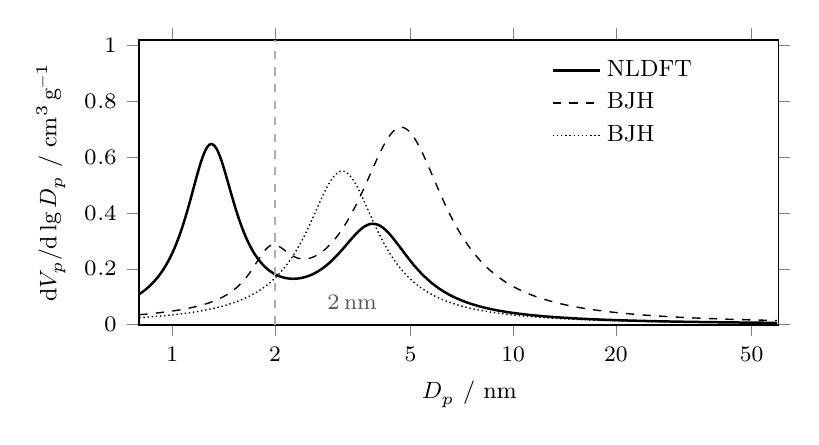
\begin{tikzpicture}
\begin{axis}[
  width=\onecolwidth, height=52mm,
  xmode=log, log basis x=10,
  xmin=0.8, xmax=60, ymin=0, ymax=1.02,
  xtick={1,2,5,10,20,50}, xticklabels={1,2,5,10,20,50},
  ytick={0,0.2,0.4,0.6,0.8,1.0},
  xlabel={孔宽 $D_p$ / nm},
  ylabel={$\mathrm{d}V_p/\mathrm{d}\lg D_p$ / $\unit{cm^3.g^{-1}}$},
  tick label style={font=\fontsize{8}{9.5}\selectfont},
  label style={font=\fontsize{8.5}{10}\selectfont},
  legend style={font=\fontsize{8}{9.5}\selectfont, at={(0.98,0.97)},
                anchor=north east, draw=none, fill=none, row sep=0.5pt},
  legend cell align=left]
% 峰形用有界函数 1/(1+((lg D-a)/w)^2)，避免小宽度指数导致 Dimension too large
\addplot[domain=0.8:60,samples=300,mainline,black]
  {0.62/(1+((log10(x)-log10(1.30))/0.090)^2)+0.34/(1+((log10(x)-log10(3.90))/0.140)^2)};
\addplot[domain=0.8:60,samples=300,thinline,black,dashed]
  {0.70/(1+((log10(x)-log10(4.70))/0.160)^2)+0.18/(1+((log10(x)-log10(1.95))/0.075)^2)};
\addplot[domain=0.8:60,samples=300,thinline,black,densely dotted]
  {0.55/(1+((log10(x)-log10(3.15))/0.130)^2)};
\legend{NLDFT（微孔＋中孔双峰）,BJH，脱附支,BJH，吸附支}
\draw[accentsoft,dashed,thinline] (axis cs:2,0) -- (axis cs:2,1.02);
\node[anchor=south west,font=\fontsize{8}{9.6}\selectfont,color=accent,
      text width=22mm,align=left] at (axis cs:2.15,0.02) {微孔上限 \qty{2}{nm}};
\end{axis}
\end{tikzpicture}
\caption{同一组等温线的两种反演结果。读者应看三处：\textbf{峰的位置}（BJH 用吸附支时中孔
峰在约 $\qty{3.2}{nm}$，用脱附支时右移到约 $\qty{4.7}{nm}$，而 NLDFT 给出约
$\qty{3.9}{nm}$）；\textbf{峰的个数}（只有 NLDFT 解出约 $\qty{1.3}{nm}$ 的微孔峰，BJH
在微孔区给不出真实信息，却可能在约 $\qty{1.9}{nm}$ 处留下一个由外推造成的虚假小峰）；
\textbf{峰高}（中孔孔容的估计值随模型变化）。三条曲线出自同一组数据，差别完全来自模型，
因此任何孔尺寸分布都必须连同模型一起报告。本图按 BJH 与 NLDFT 的典型反演行为构造，是
说明模型选择影响的示意曲线，不代表任何具体样品的实验数据。\modelmark
\figsrc{据 S1（上册）§1.2.2，书内 p.45--48 / PDF p.64--67 所述模型差异计算绘制。}}
\label{fig:psd-model}
\end{figure}

\begin{table}[htbp]
\centering
\caption{各类孔的适用分析方法与不适用方法}
\label{tab:pore-class}
{\srcsize
\begin{tabularx}{\columnwidth}{@{}llXX@{}}
\toprule
孔宽 & 名称 & 适用模型／方法 & 不适用或必须慎用（原因） \\
\midrule
$<\qty{2}{nm}$ & 微孔 &
D-R／D-A 方程、HK／SF 法、MP 法（$V$--$t$）、NLDFT &
BJH 法：Kelvin 方程在微孔内不成立，会给出 $0.5$--$2\,\unit{nm}$ 的虚假峰；
BET 面积只能称等效表面积 \\
$\qtyrange{2}{50}{nm}$ & 中孔 &
BJH／BdB、$t$ 图法、$\alpha_s$ 法、$n$ 法、NLDFT &
压汞法：只在低压段少量覆盖，小孔区受高压与接触角假设支配；
HK／SF：势能模型只对微孔标定 \\
$>\qty{50}{nm}$ & 大孔 &
压汞法、电子显微镜等直接观测法 &
氮吸附法：$\ppzero$ 接近 $1$，凝聚量测不准，Kelvin 方程不可靠 \\
\bottomrule
\end{tabularx}}
\end{table}

\begin{measure}
\textbf{气体吸附法测孔分布的条件。}（1）\textbf{吸附质选择}：$\qty{77}{K}$ 氮吸附是测
BET 表面积和中孔孔尺寸分布最常用的体系，但\textbf{不一定是测微孔孔容的最好选择}——氮
分子与分子筛孔道内阳离子之间存在较强的四极矩诱导相互作用，影响分析结果的真实性；IUPAC
建议改用惰性的球形分子 Ar（$87\,\unit{K}$）分析微孔。（2）\textbf{超低压段必须测准}：
常规吸附测量从 $\ppzero\approx0.01$ 开始，此时大部分微孔可能已经充满，因而测不到微孔
分布；高分辨低压吸附技术可从 $10^{-6}$ 甚至 $10^{-7}$ 的相对压力开始，这要求仪器有高
真空度和高精度压力传感器。（3）\textbf{脱气条件更苛刻}：排除微孔内的吸附物比中孔、大孔
困难得多。（4）\textbf{氦气截留}（helium entrapment）：商品自动吸附仪在液氮温度下用氦气
测死体积，微孔样品在此过程中会吸附相当量的氦且难以抽净，部分氦在随后吸附氮时释放，使超
低压段平衡压力偏高。解决办法是把死体积测量与微孔吸附测定分成两个独立过程：死体积测完后
重新加热脱氦，再把已测死体积作为已知参数输入仪器。（5）\textbf{避免回充气}：预处理后的
气体回充同样会使超低压段平衡压力偏高，应额外脱气或选不回填气体的分析方式。
（6）\textbf{平衡时间长}：微孔样品的平衡时间明显长于中孔、大孔样品，需放宽平衡判据
\src{S1 §1.2.2 2)，书内 p.49 / PDF p.68}。
\end{measure}

\begin{dataflow}
从一条等温线到一份可复核的孔尺寸分布：
（1）\textbf{定孔容}。纯微孔吸附剂的孔容对应 I 型等温线的平台吸附量；中微孔混合吸附剂的
微孔填充在 $\ppzero=0.01$--$0.15$ 之间完成，但此时总吸附量还含外表面上的亚单层吸附量；
IV 型等温线表明含中孔，高 $\ppzero$ 段的终止平台吸附量即中孔与更大孔的总孔容，若平台
不易分辨，总孔容通常取 $\ppzero=0.95$ 处的吸附量，对应孔宽上限 $\qty{50}{nm}$。孔容
除以样品质量得比孔容。
（2）\textbf{选模型}。微孔段用 D-R／HK／SF／MP／NLDFT，中孔段用 BJH／BdB／$t$ 图／
NLDFT，大孔段用压汞法；先由等温线类型与回滞环类型缩小范围。
（3）\textbf{反演}。按式~\eqref{eq:halsey} 或标准曲线算 $t$，按式~\eqref{eq:kelvin} 算
$r_k$，再按式~\eqref{eq:bjh-balance} 递推或按式~\eqref{eq:gae} 解积分方程，得积分分布，
求导得微分分布，取峰位为最可几孔宽。
（4）\textbf{交叉验证}。同一组数据换支（吸附支与脱附支各算一遍）、换模型、必要时换吸附质
各算一遍；分布差异大的孔宽区间不得写进结论。
（5）\textbf{报告}：按本节开头的要求，连同实验方法、$\ppzero$ 窗口与模型（含 kernel）名称
一并给出。
\end{dataflow}

\begin{pitfall}
\textbf{（1）用 BJH 分析微孔材料会得到虚假孔径峰。}高硅铝比 MFI 分子筛的高分辨低压吸附
在微孔填充段常出现台阶状跃升：骨架与氮、氩的强相互作用使微孔内吸附质由无序流体相转变为
类晶体固相，每个 MFI 单胞容纳的吸附质分子数由 23 个增至 30 个；骨架硅铝比越高、表面组成
越均匀，现象越明显（如纯硅的 silicalite-1）。此时若用 SF 法处理氩的等温线，
\textbf{或不正确地用 BJH 法处理氮的等温线（BJH 法不适用于该 $\ppzero$ 区间）}，都会得到
孔宽集中在 $0.5$--$2\,\unit{nm}$ 的虚假孔尺寸分布峰\src{S1 §1.2.2 2)，书内 p.51 / PDF p.70}。

\textbf{（2）把中孔材料的强吸附误判为微孔填充。}比表面积非常大的规整中孔材料单层吸附量
极大，低相对压力下就有显著吸附量；若把这部分吸附当成微孔填充再用 HK 或 SF 法分析，会
\textbf{人为制造出一个 $\qty{1}{nm}$ 左右、相当宽的孔尺寸分布}，而同一组数据用 $t$ 图法
作图仍是一条过原点的直线，说明它是纯中孔材料。两条判据矛盾时，以过原点直线为准，并换用
Ar 吸附复测。

\textbf{（3）脱附支在 $\ppzero\approx0.42$ 附近的伪峰。}H2(a) 型（墨水瓶孔）的回滞环在
喉管宽度小于临界尺寸时强制闭合；H3、H4、H5 型回滞环在 $\ppzero=0.4$--$0.5$ 区间同样
强制闭合。用脱附支计算时，分布曲线在 $4$--$6\,\unit{nm}$ 之间出现一个\textbf{假峰}，其
物理来源是\textbf{拉伸强度效应}（tensile strength effect）——凝聚液在张力下失稳蒸发，
而不是孔内液体真的在对应曲率下蒸发。因此\textbf{当脱附支给出的分布集中在小于
$\qty{12}{nm}$、特别是 $4$--$6\,\unit{nm}$ 时一定要慎重}：应改用吸附支对比，或采用 NLDFT
分析，还可以改变吸附温度甚至更换吸附质，最好再用直接观测法（如 TEM）确认
\src{S1 §1.2.2 1)，书内 p.47--48 / PDF p.66--67}。

\textbf{（4）压汞法在小孔区由压力与接触角假设支配。}接触角取平均 $140^{\circ}$ 在许多
情况下过于粗糙，由此导致的孔尺寸分析误差可达 $50\%$，准确结果要求汞与每种样品的接触角
实测。高压段还有两个额外贡献：汞自身被压缩的体积，以及可压缩样品在
$200$--$400\,\unit{MPa}$ 下被压紧甚至破坏。此外真实孔道常带窄喉管，汞只有达到喉管入口
半径对应的压力才能充满整个孔，算出的分布偏小于实际空腔尺寸；退汞时喉管又造成汞截留与
滞后，使退汞曲线总在进汞曲线上方。第一次进汞的低压段进汞量主要补充颗粒堆积体的体积压缩
与颗粒间隙，退汞时这部分汞不被记录，因此\textbf{第一次进汞曲线与退汞曲线不闭合，需反复
几次才闭合}。与汞形成汞齐的金属样品不适用
\src{S1 §1.2.2 2)3)4)，书内 p.58--60 / PDF p.77--79}。

\textbf{（5）不同模型给出的平均孔径不可直接互比。}各方法的孔宽定义、孔形假设（圆柱形／
平板／球形）、流体性质与积分区间都不同，得到的都是\textbf{等效模型孔的名义值}。把 BJH
脱附支的平均孔径与 NLDFT 的最可几孔宽、压汞法的孔半径写在同一张表里做趋势比较，是把模型
差异当成了材料差异；可比的前提是同一方法、同一模型、同一吸附质。

\textbf{（6）把 $t$ 图截距当作总孔容。}$V$--$t$ 曲线高段的截距只给出\textbf{中孔孔容}
（微孔吸附剂则为微孔孔容），不含大孔；大孔孔容需由压汞法或密度法给出。
\end{pitfall}

\begin{crosscheck}
\textbf{（1）与直接观测法互查。}校验 $t$ 方法与 NLDFT 最有力的办法，是用规整孔道结构的
多孔吸附剂（MCM-41、SBA-15）把直接观测结果与间接分析结果对比；对不规整孔材料，用透射
电子显微镜抽查孔宽量级，即可发现分布的明显错误（如把中孔材料报成微孔材料）。
\textbf{（2）与压汞法互查。}两法在约 $3$--$50\,\unit{nm}$ 区间重叠：吸附法在中孔段更
精细，压汞法在大孔段不可替代。若两者在同一孔宽区间给出的孔容相差数倍，应先复查预处理
条件与接触角取值，而不是取平均。
\textbf{（3）与密度、孔隙率互查。}总孔容应与由骨架密度和表观密度算出的孔隙率自洽（见下一
节）；不自洽说明孔容的积分区间没有覆盖全孔。
\textbf{（4）与表面积互查。}由孔尺寸分布积分得到的内表面积应与 BET 等效表面积同量级；
若分布积分面积远大于 BET 面积，通常意味着模型中掺入了虚假的小孔峰。
\textbf{（5）与反应数据互查。}内扩散速率受最窄喉管尺寸限制，因此分布必须能解释扩散实验
（如有效因子、Thiele 模数）的结果；若分布显示孔很大而扩散限制很强，优先怀疑模型给出了
错误的孔口尺寸，而不是怀疑扩散实验
\src{S1 §1.2.2，书内 p.44--45、p.47 / PDF p.63--64、p.66}。
\end{crosscheck}

\srcnote{本节来源：S1（上册）§1.2.2，书内 p.43--60 / PDF p.62--79。
式~\eqref{eq:kelvin}--\eqref{eq:washburn-num} 依 OCR 正文给出的变量定义与学科标准形式
重建，未逐式对照原页面图像；各式的成立条件与量纲自检见相应 \texttt{keycond} 与正文。
图~\ref{fig:psd-model} 为按模型差异计算的教学示意曲线，表~\ref{tab:pore-class} 为据正文
归纳，均非原书图表。压力--孔宽对照表与 HK／SF 法所用的吸附剂、吸附质参数见原书表 1-7
至表 1-9，本分片未逐值转录。}
}{}
\IfFileExists{chapters/parts/ch01-c.tex}{% ================================================================
%  chapters/parts/ch01-c.tex  —  第 1 章 分片 c（本章末分片）
%  §1.2.2 3)（续）其他测孔容方法、§1.2.3 颗粒度测定、
%  §1.2.4 密度测定、§1.2.5 催化剂机械强度的测定
%  源：S1（上册），书内 p.61—80 / PDF p.80—99
%  接 ch01-b.tex（孔容和孔尺寸分布）之后
% ================================================================

\paragraph{补足上一节：两种不用吸附仪的孔容测法}除压汞法与气体吸附法之外，还有两种直接而
简便的方法可以测定催化剂的孔容。它们的准确性和精确度虽然不高，但在催化研究和催化剂制备
过程中有很强的实用性。

（1）\textbf{称重法}：把已知质量的干燥催化剂颗粒在蒸馏水中煮沸几分钟，或者置于真空瓶中
彻底抽空后浸满水，使水渗入孔内；再通过小心地过滤、气吹、沥离或者在湿布上碾滚等办法除去
颗粒间隙水，然后称重，由增重与水的已知密度计算孔容。

（2）\textbf{水滴定法}：将准确称量的干燥催化剂颗粒或粉末放入锥形瓶，用滴定管滴入蒸馏水，
不断摇晃并振荡锥形瓶使水与粉末混合均匀；当粉末突然成团或者粘在瓶底不动的瞬间即为吸水
饱和终点，由滴入水量计算孔容。

这两种方法测得的\textbf{吸水容量}可直接用于等体积浸渍法和初湿浸渍法制备催化剂时计算浸渍
液的配置浓度。这是它们真正的用途：在这里孔容不是物性表征量，而是配方计算量。也正因为
如此，它们对绝对准确度要求不高，却对「颗粒间隙水是否除净」极为敏感——间隙水未除净，就把
堆积空隙算成了孔容，结果系统性偏大；而水滴定法的终点判据是人为目视判断，重复性取决于
操作者。\src{S1 §1.2.2 3)，书内 p.61 / PDF p.80}

\subsection{颗粒度测定}

\begin{probout}
\textbf{本节回答}：「催化剂颗粒有多大」这句话在什么意义上可以被量化；一个粒径数值要连同
哪些条件才能被复核；以及为什么两台仪器测同一批样品可以差出两三倍。

\textbf{输出}：颗粒体系的\textbf{平均粒径}与\textbf{粒度分布}（含百分数基准、特征值
$D_{50}$、$D_{97}$、边界粒径与分布宽度指标），以及\textbf{所依据的等效粒径定义与测定
方法}。

\textbf{本节核心判断}：颗粒度测定测的不是几何尺寸，而是\textbf{等效量}。真实颗粒形状多
为不规则体，用一个或几个尺度数值去描述其尺寸特征是不现实的。因此表达颗粒度的方法放弃了
采用任何颗粒形状的概念，而引入\textbf{等效粒径}：当被测定颗粒的某种几何学特性（投影、
体积、表面积）、物理性质（光学、电学、质量）、物理行为（流体动力学、空气动力学）或者
化学吸附特性与某一直径的同质球体最相近时，就把该球体的直径作为被测颗粒的等效粒径。由此
推出本节两条结论：（i）\textbf{描述粒径及其分布必须同时说明依据的规则和测量的方法}，少了
任何一项，数值都不可复核；（ii）不同原理测的是\textbf{不同的等效直径}——体积等效、面积
等效、Stokes 等效、散射等效彼此不能换算，\textbf{换方法得到的数值不可直接互比}。
\end{probout}

\subsubsection{颗粒、一次颗粒与二次颗粒}

「颗粒」是指在毫米到纳米尺寸范围内具有特定形状的几何体；多相催化研究的一般是固体颗粒。
对单颗粒而言，颗粒度（particle size）指颗粒的大小。但在多相催化研究领域中，「颗粒」一词
所指的对象丰富而复杂。

狭义的催化剂（工业催化剂、实用催化剂）颗粒——球（sphere）、条（pellet、cylindrical）、
片、三叶草条（trilobe）等——是指人工成型的、具有发达孔系的颗粒聚集体。\textbf{工业催化剂
颗粒度}是指在操作条件下，催化剂颗粒\textbf{不再人为分开的最小基本单元}的大小或尺寸。
当催化剂颗粒具有显著的几何尺度（如毫米级）和确定的几何特征（如球体、圆柱体、环、三叶草
条等模状）时，催化剂的尺寸以其实际几何特征尺度标示——这是唯一可以直接用尺子量的情形。

更多的情况下，多相催化研究的「颗粒」以单晶、微粒、粉体及分散在载体上的金属或化合物粒子
等分散体系形态出现。其中：

\begin{itemize}
\item \textbf{一次颗粒}（primary particles）：原子、分子、离子按晶体结构的规则形成的单晶
粒子，通常是纳米级的；
\item \textbf{二次颗粒}（secondary particles）：若干晶粒聚集成的大小不一的微米级颗粒；
\item \textbf{粉体}（powder）：细小固体颗粒的集合。
\end{itemize}

这一区分在催化剂研究中是硬约束：X 射线衍射线宽化法测的是\textbf{晶粒}（一次颗粒），
显微镜法测的是\textbf{投影轮廓}，沉降法与激光散射法测的是\textbf{分散在介质中的颗粒或
团聚体}（二次颗粒）。三者测的常常不是同一个对象，因此三者的数值本来就不该相等
\src{S1 §1.2.3 1)，书内 p.61--62 / PDF p.80--81}。

\subsubsection{等效粒径：粒径必须连同方法一起报告}

\begin{principle}
\textbf{等效粒径的定义。}当被测定颗粒的某种几何学特性（投影、体积、表面积）、物理性质
（光学、电学、质量）、物理行为（流体动力学、空气动力学）或者化学吸附特性等性质与某一直径
的同质球体最相近时，就把该球体的直径作为被测颗粒的等效粒径。

\textbf{粒度分布。}研究的对象是一个粒子数量庞大的颗粒体系（集合），被研究的颗粒并不总是
绝对一样大小，有时大小分布甚至覆盖几个数量级。测量其中单颗颗粒的粒径没有意义，需要获得的
是关于颗粒体系\textbf{平均粒径}及\textbf{粒度分布}的总体信息。因此对颗粒体系而言，
「颗粒度」同时具有平均粒径大小和粒度分布双重含义。

\textbf{平均粒径的通式。}设粒度频率分布函数为 $f=q(x,n)$，$x$ 为粒径；$n=0$ 为个数分布
函数，$n=2$ 为面积分布函数，$n=3$ 为体积或质量分布函数，则
\begin{equation}\label{eq:ch01c-dn}
\bar{D}(n)=\frac{\int_{0}^{\infty}x^{n}f(x)\,\mathrm{d}x}{\int_{0}^{\infty}f(x)\,\mathrm{d}x}
\end{equation}
但更多情况下只能得到粒度\textbf{区间}分布的数据而非分布函数，这时平均粒径按下式计算：
\begin{equation}\label{eq:ch01c-dpq}
\bar{D}[p,q]=\left[\frac{\sum_{i}n_{i}d_{i}^{p}}{\sum_{i}n_{i}d_{i}^{q}}\right]^{\frac{1}{p-q}}
\end{equation}
式中 $n_i$ 为颗粒粒径分级第 $i$ 组级区间上的颗粒数；$d_i$ 为第 $i$ 组级颗粒的直径典型值，
取组级区间上、下限的几何平均值
\begin{equation}\label{eq:ch01c-di}
d_{i}=\sqrt{D_{i}D_{i+1}}
\end{equation}
$D_i$ 为该区间的下限粒径数值，$D_{i+1}$ 为上限粒径数值。

常用的几个特例是：个数平均粒径 $D[1,0]$（算术平均粒径）、个数表面积平均粒径
$D[2,0]$、个数体积平均粒径 $D[3,0]$、\textbf{表面积平均粒径} $D[3,2]$（Sauter 平均粒径）
与\textbf{体积（质量）平均粒径} $D[4,3]$（de Brouckere 平均粒径）。由
式~\eqref{eq:ch01c-dn} 可见它们与 $\bar{D}(n)$ 的关系是
\begin{equation}\label{eq:ch01c-d32a}
D[3,2]=\bar{D}(2),\qquad D[4,3]=\bar{D}(3)
\end{equation}
在很多情况下颗粒的粒径\textbf{个数}分布是得不到的，得到的是粒径面积、粒径体积或者粒径
质量分布，则此时
\begin{equation}\label{eq:ch01c-d32}
D[3,2]=\frac{\sum_{i}v_{i}}{\sum_{i}\left(v_{i}/d_{i}\right)},\qquad
D[4,3]=\frac{\sum_{i}w_{i}d_{i}}{\sum_{i}w_{i}}=\frac{\sum_{i}v_{i}d_{i}}{\sum_{i}v_{i}}
\end{equation}
式中 $v_i$（或质量 $w_i$）为颗粒粒径分级第 $i$ 组级区间上的总颗粒体积（质量），$d_i$ 仍
取该区间上、下限的几何平均值。

\textbf{这两式的意义。}$D[3,2]$ 是「总表面」与「总体积」之比决定的平均径，它是与比表面
积、传质、催化反应速率最直接相关的一个平均径；$D[4,3]$ 是体积加权平均径，它被大颗粒
支配，是激光粒度仪默认报出的那个数。两者相差多少，完全取决于分布的宽度：分布越宽，差别
越大。

\textbf{这两式的原书对应式。}此处已对照原页面图像（书内 p.63 / PDF p.82）：原书式 (1-54)、
(1-55) 印 $D[3,2]=\frac{\sum_{i}s_{i}d_{i}}{\sum_{i}s_{i}}$、
$D[4,3]=\frac{\sum_{i}w_{i}d_{i}}{\sum_{i}w_{i}}$，其变量说明段作「$s_{i}$ 和 $w_{i}$ 为颗粒粒径
分级第 $i$ 组级区间上的总颗粒面积和总颗粒体积（质量）」，可见原书确有面积形式的
$D[3,2]$。本处式~\eqref{eq:ch01c-d32} 改用体积（质量）分数写出，两者在全区间上等价：球形
颗粒的 $s_{i}\propto v_{i}/d_{i}$，形状系数在分子分母中相消，故
$\sum_{i}s_{i}d_{i}/\sum_{i}s_{i}=\sum_{i}v_{i}/\sum_{i}(v_{i}/d_{i})$；保留体积形式是为了能直接
对接激光粒度仪默认报出的体积基准分布。
\end{principle}

\begin{measure}
\textbf{必须同时报告的三件事。}（1）\textbf{等效粒径的定义}（体积等效、面积等效、
Stokes 等效、散射等效……）；（2）\textbf{分布所依据的百分数基准}——个数基准（count
basis）、面积基准（surface basis）、体积基准（volume basis）还是质量基准（mass
basis）；（3）\textbf{测定方法与制样分散条件}。同样一批 γ-氧化铝粉，图像法给出的是个数
基准的投影径分布，激光散射法给出的是体积基准的散射等效径分布，两者不仅\textbf{中位径
不同}，连\textbf{分布形状}都不同——因为从个数基准换算到体积基准要乘 $d^{3}$，这一步会
把大颗粒的权重急剧放大。\src{S1 §1.2.3 2)，书内 p.62--63 / PDF p.81--82}
\end{measure}

\subsubsection{粒度分布的表达与特征指标}

粒度分布（particle size distribution）就是用特定的方法表示颗粒体系中不同粒径颗粒占颗粒
总数（总量）的比例，反映粒子大小的均匀程度。表达上有两种基本形式：\textbf{频率分布}
（又称微分分布或区间分布，给出与各粒径相对应的颗粒在体系中所占的百分数）与\textbf{累积
分布}（又称积分分布，表示小于或大于某粒径的颗粒所占的百分数）。百分数的基准可用个数
基准、面积基准、体积基准和质量基准等表示——\textbf{同一组颗粒，换一个基准就是另一条
曲线}。

粒度分布可用表格、图形和函数三种形式表示：表格法即用列表方式给出某些粒径所对应的百分比；
图形法是在直角坐标系中用直方图和曲线等图形表示；函数法则用函数表示，如
Rosin--Rammler 分布函数、正态分布函数等。

表示粒度分布特性的关键指标有：

\begin{itemize}
\item \textbf{平均粒径}（mean particle size）：通过对粒度分布加权的平均粒度的量，即
式~\eqref{eq:ch01c-d32a} 与式~\eqref{eq:ch01c-d32} 给出的一族数值。
\item \textbf{$D_{50}$}：一个样品的累积粒度分布百分数达到 50\% 时所对应的粒径。它的物理
意义是粒径大于它的颗粒占 50\%，小于它的颗粒也占 50\%。$D_{50}$ 也称中位粒径或中值粒径
（median particle size）。\textbf{注意它对应的是「累积到一半」，不是「出现最多」}。
\item \textbf{$D_{97}$}：累计粒度分布数达到 97\% 时所对应的粒径，物理意义是粒径小于它的
颗粒占 97\%。$D_{97}$ 常用来表示粉体\textbf{粗端}的粒度指标；类似地还有 $D_{90}$、
$D_{3}$ 等。
\item \textbf{最频值}（mode）：频率曲线最高点所对应的粒径值，也称最可几粒径。
\textbf{最频值与 $D_{50}$ 只有在分布对称时才重合}；对常见的右偏分布（大颗粒拖尾），最频
值小于 $D_{50}$。
\item \textbf{边界粒径}：用来表示样品粒度分布的范围，由一对特征粒径组成，如
（$D_{10}$，$D_{90}$）或（$D_{3}$，$D_{97}$）。
\item \textbf{分布宽度}：工程上常报「跨度」（span）$=(D_{90}-D_{10})/D_{50}$。$D_{50}$
只说明「一半颗粒比它小」，跨度才说明「分布有多宽」。只报 $D_{50}$ 而不报跨度，等于只报了
分布的一个点。此处已对照原页面图像（书内 p.63 / PDF p.82）：原书「表示粒度分布特性的关键
指标」下确只列平均粒径、$D_{50}$、$D_{97}$、最频值（mode）与边界粒径五项——其中边界粒径举例
为「（$D_{10}$，$D_{90}$）、（$D_{3}$，$D_{97}$）」，$D_{97}$ 条附「类似地，还可以有 $D_{3}$、
$D_{10}$、$D_{90}$ 等」——原书未给出「跨度」；跨度 $=(D_{90}-D_{10})/D_{50}$ 是本节的工程惯用
补充，且原书对最频值只说「频率曲线的最高点所对应的粒径值，也称最可几粒径」，未涉及它与
$D_{50}$ 的关系。
\end{itemize}

\src{S1 §1.2.3 2)，书内 p.62--63 / PDF p.81--82}

\subsubsection{测定方法与各自的等效口径}

等效粒径的概念决定了颗粒度的测定已经失去了通常的几何学测量的意义，而转化为材料物理、
化学性能的测试分析。因此，描述粒径及其分布必须同时说明依据的规则和测量的方法。

实验室常用的颗粒度测定方法很多：筛分法、显微镜（图像）法、重力沉降法、离心沉降法、库尔特
（电阻）法、小角激光光散射法、动态光散射法、电镜法、氮气吸附（BET）法等。要选择合适的
测定方法，依次考虑三件事：首先，颗粒材料的物化性质；其次，其测量上下限要能够覆盖所关心
或者欲研究的颗粒尺寸范围；最后，测量条件尽可能接近材料的使用条件，即对材料的应用有充分
敏感性。\src{S1 §1.2.3 3)，书内 p.63--65 / PDF p.82--84}

表~\ref{tab:ch01c-methods} 把常用方法的等效口径、分布基准、适用范围与主要局限并列在一起。
读这张表请从右往左读：先确认样品的粒径落在哪一行的方法量程内，再看该行的「关键局限」是否
正好命中自己的样品，最后才看「等效粒径」一列——那一列才是数值能不能与文献比较的判据。

{\srcsize
\setlength{\tabcolsep}{3pt}
\begin{longtable}{@{}p{26mm}p{44mm}p{26mm}p{62mm}@{}}
\caption{实验室常用粒度分析方法及其特点。\textbf{读者应重点看第二列与第四列}：第二列说明
该法给出的是哪一种等效直径、以什么为基准的分布；第四列说明在什么情况下这个数值会失真。
凡是第二列不同或基准不同的两个数值，都不可直接互比。「适用粒径范围」一列的量程照录原书
表 1-10，实际可测范围还取决于仪器型号与制样条件。\src{据 S1 表 1-10 与 §1.2.3 3)，
书内 p.64—65 / PDF p.83—84 整理。}}
\label{tab:ch01c-methods}\\
\toprule
方法 & 等效粒径与分布基准 & 适用粒径范围 & 关键局限与适用条件 \\
\midrule
\endfirsthead
\toprule
方法 & 等效粒径与分布基准 & 适用粒径范围 & 关键局限与适用条件 \\
\midrule
\endhead
\bottomrule
\endlastfoot
筛分法 & 物理筛分等效径；\textbf{质量}（体积）分布 & 38 — 6000 µm（标准筛）；非标准筛可至 $3\times10^{5}$ µm & 下限 38 µm（Tyler 400 目），更细的颗粒测不了；颗粒能否通过取决于取向、筛面运动形式、物料载荷与筛分时间，重复性差；不适于黏性物质与易碎样品，杆状粒子误差大 \\
光学显微镜法 & 几何学等效径（投影面积圆等效径即 Heywood 径）；\textbf{个数}分布 & 约 1 — 6000 µm & 代表性差、重复性差；人工图像分析工作量大、随意性大、速度慢；形状规整且分布窄时测几百个颗粒即可，形状极不规则且分布宽时需测数万个 \\
电子显微镜法（SEM／TEM） & 几何学等效径；\textbf{个数}分布 & 约 0.001 — 5 µm（原表按倍率给出：光学显微镜 1 µm 起、SEM 0.01 µm 起、TEM 0.001 µm 起，均未给上限，此处上限为常见仪器的实用值） & 观察的颗粒数极少，代表性最差；TEM 测到的是晶粒（一次颗粒）与负载金属纳米粒子，不是二次颗粒；制样与取样误差常大于测量误差 \\
沉降法（重力） & Stokes 径（\textbf{流体动力学等效径}）；\textbf{质量}分布 & 10 — 300 µm & 只适用于球形颗粒的滞流沉降（$Re<1$，放宽也不超过 $2$）；仅适用于单分散体系，要求恒温；不规则颗粒的 Stokes 径小于几何学等效径；$d<0.5$~µm 时布朗运动严重干扰 \\
沉降法（离心／X 光透过） & Stokes 径；\textbf{质量}分布 & 0.1 — 300 µm & 离心沉降以离心加速度替代重力，拓宽了测量下限；可见光透过法下限 $>5$~µm（细颗粒散射），低能 X 射线可到 0.1 µm，但不适于高吸收 X 射线物质与强磁性材料 \\
电阻法（库尔特原理） & 球\textbf{体积}等效径；个数或体积分布 & 约 0.4 — 1200 µm & 单只小孔管只能测其孔径的 2\%—60\%，大小颗粒之比大于 30 时需多量程，归一化带来误差；大颗粒易堵小孔管；不适于多孔颗粒、密度大或憎水的样品；颗粒带电会使结果失真 \\
小角激光光散射法 & 等效散射径；\textbf{体积}分布（默认报 $D[4,3]$） & 0.02 — 3000 µm & 需预知颗粒折光指数（混合样品只能取主要物质的）；分辨率低，对较均匀的样品给不出精确分布；颗粒形状越不规则、分布越宽，误差越大；要求单散射，对浓度与分散有要求 \\
动态光散射法 & 流体动力学等效径；\textbf{强度加权}粒径分布（体积／数量分布须模型换算） & 0.0001 — 10 µm & 主要覆盖纳米与亚微米级；由 Einstein--Stokes 方程求径一步不引入与颗粒性质有关的参数（只需温度与黏度已知），但强度到体积／数量的换算须另设形状、光学性质与散射模型假设，不能与电镜个数分布直接比较峰面积；$z$ 平均径与 PDI 是累积量分析给出的平均量与宽度指标，与分布反演及其他平均径不可混用；要求样品池中颗粒浓度低并保持高分散；对入射光单色性要求高，须用激光光源 \\
电泳法 & 电泳迁移率 $\mu_{\mathrm{e}}$ 与 Zeta 电位 $\zeta$（\textbf{不给出粒径分布}） & 0.005 — 30 µm & 电泳光散射测的是迁移率，再由电泳模型求 $\zeta$；由 $\mu_{\mathrm{e}}$ 或 $\zeta$ 反演粒径必须附加含尺寸的模型并在报告中说明，薄双电层 Smoluchowski 极限 $\mu_{\mathrm{e}}=\varepsilon\zeta/\eta$ 与粒径无关（同 $\zeta$ 的 100 nm 与 200 nm 球给出同一 $\mu_{\mathrm{e}}$）；仪器同时报出 Zeta 与粒径时，粒径来自 DLS 通道或另行测定，不能把 $\mu_{\mathrm{e}}$ 当作唯一反演依据；只适用于能在液相中稳定分散且带电的颗粒；结果对介质离子强度、pH 与颗粒表面状态敏感，测量条件必须与使用条件一致 \\
BET 比表面积法 & \textbf{表面积}等效径 $D[3,2]$（单值） & 0.03 — 1 µm & 由 $D=6/(S\rho)$ 得到的只是一个平均径，\textbf{给不出任何分布}；富含微孔的颗粒必须用外比表面积计算，否则数值无意义 \\
空气透过法 & 表面积等效径（Kozeny--Carman 方程） & 0.2 — 75 µm & 相对测量方法，不能精确反映真实粒径；不适于多孔固体；一般只用于无孔大颗粒材料的工艺过程与产品质量监控（水泥、冶金、建材行业有标准） \\
X 射线衍射线宽化法 & Scherrer 等效径（\textbf{晶粒}体积平均尺寸） & 5 — 50 nm & 测的是晶粒（一次颗粒），不能反映二次颗粒的粒度；有微应变与仪器宽化时必须先分离 \\
化学吸附法 & 由分散度换算的活性组分粒径 & 约 0.1 — 10 nm & 利用化学吸附的选择性，只适用于负载型催化剂的活性组分；结果通常以\textbf{分散度}表示，无粒度分布数据 \\
\end{longtable}}

\noindent 上表已对照原页面图像逐格核对：原书表 1-10 为 9 行 4 列（方法／原理、等效粒径和
分布／工具或仪器／测试范围 µm），本表保留其中方法、等效粒径与分布基准、测试范围三列，
未保留「工具或仪器」列；「测试范围」一列的量程已按原表数值逐行改写（如电泳法
$0.005$—$30$ µm、动态光散射法 $0.0001$—$10$ µm、BET 比表面积法 $0.03$—$1$ µm、
筛分法 $38$—$6000$ µm 而标准筛以外的筛具可至 $3\times10^{5}$ µm）；表末的
X 射线衍射线宽化法与化学吸附法两行为本表所增，不在原表之内；「关键局限」列为正文各段
叙述的归纳，不是原表栏目。\src{S1 表 1-10，书内 p.64 / PDF p.83}

下面按原理把这条线索串起来。

\paragraph{筛分法}是一种最传统、应用最广的粒度测定方法，使颗粒通过不同尺寸的筛孔来测试
粒度。筛分法分干筛和湿筛，可以用单个筛子控制单一粒径颗粒的通过率（质量），也可以用一垛由
粗到细按筛号顺序叠起的筛子同时测量多个粒径颗粒的通过率，计算质量分数，获得\textbf{以质量
为基准}的筛分粒径分布及平均粒径。筛分法所得的\textbf{筛分径}（sieving diameter）以颗粒
通过和被截留的粗、细筛孔直径的均值表示，是典型的「筛分等效径」。

筛子有网筛和板筛两种，网筛的网目由金属丝按正方形编织而成。筛子的规格（筛号）用筛孔尺寸
表示；筛号还常用「目」（mesh）表示，「目」指在筛面的每英寸（1 英寸 = 2.54 厘米）长度上
开有的筛孔数目。由于编网所用筛丝直径不同，筛孔大小也不同，不同国家、不同行业的筛网规格有
不同标准，\textbf{同一目数筛子的筛孔尺寸可能不一样}。因此用目数标示筛子筛号时必须同时
标明筛孔尺寸。标准筛是按法令规格化的一套筛具，我国尚未颁布国家标准套筛，目前国际上常用
ISO 系列和美国 Tyler 系列；Tyler 系列最细的是 400 目，筛孔尺寸 38 µm。因此
\textbf{筛分法测定范围在 38 µm 以上}，粒度大于数毫米的物料所用的筛子一般为非标准筛。
筛分法的优点是工具便宜、操作简单；分析样品量大，代表性强，数据统计精确度高；能直接提供
粒径质量分布。缺点是下限只有 38 µm，不能分析细颗粒；难以分析黏性物质，不能分析易碎颗粒
样品；分析非规则形状（如杆状）粒子误差大；筛分结果受筛分时间影响大，重复性差；速度慢、
耗时。\src{S1 §1.2.3 3)1)，书内 p.65--66 / PDF p.84--85}

\paragraph{显微镜法}直接观察个别颗粒，根据颗粒投影像测得投影径，获得以个数、面积为基准的
粒度分布。光学显微镜可以测定微米级的颗粒，电子显微镜（SEM、TEM）可以测定纳米级的颗粒和
晶粒。投影径是几何学等效粒径，常用的表示方式是\textbf{投影面积圆等效粒径}
（equivalent circular diameter），即与粒子的投影面积相同圆的直径，也称为 Heywood 径。
其他几何学等效粒径还有：

\begin{itemize}
\item \textbf{Martin 径}：又称定方向等分径，是指在指定方向上，将颗粒投影面积等份分割的
弦线的长度；
\item \textbf{Feret 径}：任意方向上与颗粒投影面相切的一对平行线间的距离；通常指其中最宽
的一对平行线间的距离；
\item \textbf{Krumbein 径}：又称同方向最大径，指在指定方向上，颗粒投影轮廓内最长弦线的
长度。
\end{itemize}

对不规则颗粒，各粒径值之间一般存在关系：Feret 径 $\geq$ Krumbein 径 $\geq$ Heywood 径。
这一点有直接的实操含义：\textbf{同一张显微照片，用不同的「量法」就会得到系统性不同的
数值}，因此图像法报告必须写明所用的是哪一种投影径。为提高可靠性和代表性，显微镜法要求
观察和测量足够多的颗粒数目：形状规整、粒度分布窄的颗粒测几百个就足够；形状极不规则、
分布很宽的则需测数万个。显微镜法的优点是光学显微镜便宜，可直接观察颗粒形状和颗粒团聚，
透射电镜还可以测定负载型催化剂载体上金属或氧化物的纳米晶粒；缺点是代表性差，重复性差，
只适合测定粒度分布窄的样品，且操作烦琐、人工图像分析工作量大。\src{S1 §1.2.3 3)2)，
书内 p.66--67 / PDF p.85--86}

\paragraph{沉降法}建立在悬浮颗粒的动力学稳定性与粒径的关系上：颗粒较小时分子热运动产生的
布朗运动起主要作用，分散体系趋于稳定；颗粒较大时重力产生的沉降破坏分散体系的稳定性。
在自然重力状态下，若一个表面光滑的球形颗粒在静止流体中\textbf{滞流沉降}（颗粒所受重力、
浮力和运动阻力平衡，匀速沉降），则沉降速度与粒径的关系用 Stokes 公式描述：

\begin{equation}\label{eq:ch01c-stokes}
u=\frac{(\rho-\rho_{0})\,g\,d^{2}}{18\eta}
\end{equation}

式中 $d$ 为颗粒直径；$\eta$ 为流体黏度；$\rho$ 为颗粒真密度；$\rho_0$ 为流体密度；
$u$ 为颗粒的沉降速度；$g$ 为重力加速度。当雷诺准数 $Re=d u \rho_{0}/\eta<1$ 时沉降形态
为滞流（严格地应满足 $Re<0.2$，但也可放宽至 $Re<2$）。Stokes 公式表明\textbf{沉降速度与
颗粒直径的平方成正比}，大颗粒沉降快、小颗粒沉降慢；沉降法就是根据颗粒在液体中沉降速度
不同来测量粒径和粒度分布的方法。

Stokes 公式描述的是球形颗粒的滞流沉降行为。由于沉降阻力与颗粒受力的有效面积有关，对不规
则颗粒，其表面粗糙程度、形状及投影面积均影响沉降速度和沉降形态。由沉降法测得的粒径称为
\textbf{Stokes 径}，相当于在流体中与该颗粒具有\textbf{相同沉降速度}的同质球形颗粒的直径，
属于流体动力学等效粒径。对不规则颗粒体系，颗粒形状与球形的差异程度越大，沉降法测得的
Stokes 径与几何学等效粒径差异也就越大（Stokes 径偏小）。

一般对颗粒而言加速阶段时间很短，通常忽略，可以认为整个沉降过程是匀速的。沉降速度
$u=H/t$（$H$ 为沉降高度，$t$ 为沉降时间），由此自然重力状态下的 $d$--$t$ 函数为

\begin{equation}\label{eq:ch01c-dt-g}
d=\left[\frac{18\eta H}{(\rho-\rho_{0})\,g\,t}\right]^{1/2}
\end{equation}

在重力场中细颗粒的沉降速度很小，现代沉降仪大多引入\textbf{离心沉降}方式：离心加速度远
大于重力加速度，粒径相同时离心沉降的测试时间大大缩短。离心沉降速度的表达式在形式上与
重力沉降式一样，只是以离心加速度代替重力加速度：

\begin{equation}\label{eq:ch01c-centrif}
u_{r}=\frac{(\rho-\rho_{0})\,\omega^{2}r\,d^{2}}{18\eta}
\end{equation}

式中 $\omega$ 为转动的角速度，$r$ 为颗粒距转动中心的距离，$u_r$ 为颗粒的离心沉降速度。
离心沉降时颗粒的实际运动轨迹是一个半径逐渐扩大的螺旋线，但由于颗粒和流体同时做圆周
运动，二者在切向上相对静止，所以\textbf{离心沉降速度并不是颗粒的实际运动速度，只是其在
径向上的分量}。当颗粒匀速沉降时离心力与摩擦阻力达到平衡；经时间间隔 $t$，颗粒由距转动
中心 $r_1$ 运动至 $r_2$ 处，积分整理后离心力状态下的 $d$--$t$ 函数为

\begin{equation}\label{eq:ch01c-dt-c}
d=\left[\frac{18\eta\,\ln\left(r_{2}/r_{1}\right)}{(\rho-\rho_{0})\,\omega^{2}t}\right]^{1/2}
\end{equation}

直接测量颗粒的沉降速度很困难，但通过测量颗粒体系沉降过程的\textbf{浓度变化}可以间接求得
沉降速度。依据浓度测定方法，常见的沉降测定法有移液管法、沉降天平法、沉降管法、比重计法、
光透过重力（离心力）沉降法和 X 射线透过重力（离心力）沉降法等。其中移液管法
（pipette analysis）是把颗粒均匀分散的沉降液转入带固定位置移液管的 Andreassen 容器，令其
自由沉降，在适当时间从一定高度处抽吸一定量的悬浊液，烘干并精确称量其中的固体质量，按
Stokes 公式把时间换算成粒径，由干重变化求粒度分布；光透过法则令沉降液自由沉降，用光强
变化率间接反映沉降速度，光的透过量与浓度的关系符合 Lambert--Beer 定律。
\src{S1 §1.2.3 3)3)，书内 p.67--70 / PDF p.86--89}

\begin{measure}
\textbf{沉降法的条件清单。}（1）\textbf{浓度}：沉降液中颗粒质量分数最好控制在 0.1\%—3\%，
否则颗粒间的相互作用会干扰沉降过程；颗粒间距离大于粒径 10 倍、沉降容器尺寸大于粒径
100 倍时，颗粒干扰和器壁效应可忽略。（2）\textbf{介质匹配}：被测颗粒不应在分散介质中
溶解、溶胀；需调节分散介质的密度和黏度与固体颗粒的密度和尺寸相匹配；不易润湿的颗粒还需
加入表面活性剂增大固液亲和力。（3）\textbf{滞流条件}：对于密度或粒径很大的颗粒，沉降
速度太快会进入过渡流或湍流区，Stokes 公式不再适用，体系\textbf{最大}颗粒的沉降雷诺准数
必须满足滞流条件。（4）\textbf{温度}：测定过程要求维持恒定温度。（5）\textbf{下限}：
非常微细的颗粒（如 $d<0.5$~µm）在介质中的布朗运动会严重干扰沉降，沉降法也无法测定；
重力沉降的粒径范围为 10—300 µm，离心沉降为 0.1—10 µm。光透过法的悬浮液质量百分浓度
以 0.02\%—1\% 为好，可见光检测细颗粒时发生光散射，测量下限大于 5 µm，且可见光强度较弱、
灵敏度低；选用低能 X 射线作入射光源可把下限推到 0.1 µm，但不适于分析高吸收 X 射线物质
和强磁性材料。\src{S1 §1.2.3 3)3)，书内 p.69--70 / PDF p.88--89}
\end{measure}

\paragraph{电阻法}的工作原理是：悬浮在电解液中的不导电颗粒随电解液流入一个负压的孔管，
当其流经小孔时，颗粒体积排除了相同体积的电解液，导致孔口处电阻发生瞬时变化；在孔管内外
设有电极，通过一个恒电流电路记录产生的电位脉冲。库尔特原理指出\textbf{电阻变化的大小与
颗粒的体积成正比}，因此电位脉冲信号的大小和次数与颗粒的体积大小和数目成正比。库尔特计数
法获得的是\textbf{球体积等效粒径}，其分布以个数或体积为基准。

库尔特计数法单只小孔管（对应一个量程）可测量的颗粒尺寸范围在其孔直径的 2\%—60\%；当
样品粒度分布较宽（大、小颗粒之比大于 30）时需使用多只小孔管分别测量。仪器提供的孔直径
一般为 15—2000 µm，量程约 0.4—1200 µm，测量速度最高可达每秒 10000 个颗粒。它以体积
等效粒径表征颗粒粒径，\textbf{不受颗粒形状影响}；它一个个地测量每个颗粒的大小，因而
分辨率很高，并能给出颗粒的绝对数目，特别适用于检测液体中的稀少颗粒；重复性好，分析不受
分散剂、悬浮液折光率、颜色、形态的影响。缺点是对样品要求苛刻：必须可分散并悬浮在电解液
中，因此无法测量相对密度较大的物质颗粒和憎水的有机材料；如果样品颗粒带电，会抵消其体积
占用造成的电阻增加，造成测量失真；动态范围小，宽分布样品虽可多管测量，但数据归一化会
带来误差，且大颗粒容易堵塞小孔管（孔口越小越易堵）；\textbf{不适宜测量多孔性颗粒}。
\src{S1 §1.2.3 3)4)，书内 p.70--71 / PDF p.89--90}

\paragraph{小角激光光散射法}（又称激光光衍射法）属于静态（弹性）光散射，仪器常称为激光
粒度仪。光束行进方向上的颗粒障碍物对光有散射作用，会使一部分光偏离原来的传播方向而向
四周传播；散射角的大小与颗粒尺寸有关——\textbf{颗粒越小，散射角越大}，而散射光的强度
包含颗粒的含量信息。该法把颗粒均匀地放置到激光光束中，用光电探测器在不同角度上测量散射
光强度，数据经理论处理得到粒度分布。

散射理论分两支。对于粒径远大于入射光波长的球形颗粒体系，可以认为所有颗粒对光线具有相同
的散射效率，颗粒的透光性也可忽略，此时 \textbf{Fraunhofer 衍射理论}是解析光散射数据的
简便方法：大颗粒对光的散射角很小，散射光强度与颗粒投影面积（粒径的平方）和数量成正比。
当颗粒直径接近入射光波长时，更多的光被散射到很大的角度，散射光强度与颗粒大小、折光率及
入射光强度之间存在复杂关系；而当颗粒直径远小于入射光波长时（Rayleigh 区），散射变成各向
同性，此时在材料、介质、波长与颗粒个数都相同的条件下，散射光强度与粒径的六次方\textbf{成
正比}——粒径由 10 nm 增至 20 nm，散射强度增大 $2^{6}=64$ 倍。原书此处排印为「成反比」，
与 Rayleigh 散射的 $I\propto d^{6}$ 关系相反，属原书笔误，本版按正比表述并在此记明。这时需用
\textbf{Mie 散射理论}描述散射光场强度分布——它由
Maxwell 电磁波方程严格推导，适用于计算任意大小的颗粒，可在很宽的粒度范围内得到完全精确的
结果（约 0.02—3000 µm），而 Fraunhofer 理论只是粒径远大于光波长情况下散射现象的近似和
简化描述。早期受计算能力限制，激光光衍射分析法只能使用 Fraunhofer 近似（这也是该法称为
「衍射法」的原因），探测器阵列角度也较小，只能测微米以上颗粒；目前先进仪器大多全量程使用
Mie 理论，同时采用多激光光源（短波长）、增加大角与背散射光电探测器、偏振光强度差散射
（PIDS）等技术改善分辨率与下限。

Mie 散射理论假设散射颗粒是球形，散射光强度与颗粒体积相关；小角激光光散射法正是利用颗粒
对激光的散射特性做等效对比来测定\textbf{等效散射径}（与实际被测颗粒具有相同散射效果的
球形颗粒的直径）。因此实际测量中不规则颗粒的形状、粒径分布特性对最终结果影响较大，颗粒
形状越不规则、粒径分布越宽，分析结果误差越大（引入非球形颗粒校正的 Mie 公式可用于不规则
颗粒）。该法得到的是\textbf{体积分布}，平均粒径是体积平均粒径 $D[4,3]$。由于 Mie 理论
假设散射光是不相关的单散射，实际测量对样品池中颗粒的浓度和分散情况有一定要求，以降低复
散射或相干散射的影响；小颗粒的散射与其材料的光学性质关系密切，Mie 理论需要预知颗粒的
折光指数（有系数匹配、折光仪和平均值等确定方法，混合样品可取主要物质的折光指数）。该法
测量速度快、动态范围大、操作简便、重复性好、应用领域广（不仅能测固体颗粒、乳胶颗粒，而且
可测雾滴、气泡等的粒度），但\textbf{分辨率低}，对于颗粒较均匀的样品不能给出精确的粒径
分布。\src{S1 §1.2.3 3)5)，书内 p.71--73 / PDF p.90--92}

\paragraph{动态光散射法}（dynamic light scattering，也称准弹性光散射 QELS 和光子相关
光谱 PCS）是研究纳米颗粒粒度分布的有力手段（1—500 nm）。前述小角激光光散射法可以理解为
静态光散射；对于远小于光波波长的亚微米级颗粒（$<250$~nm），由瑞利散射理论可知，散射光
相对强度的角分布与粒子大小\textbf{无关}，不能通过对散射光强度的空间分布来确定颗粒粒度，
而动态光散射正好弥补这一不足。

纳米颗粒在流体中布朗运动的速度与颗粒的大小有关，符合 Einstein--Stokes 方程
\begin{equation}\label{eq:ch01c-einstein}
D_{\mathrm{d}}=\frac{kT}{6\pi\eta R}
\end{equation}
式中 $D_{\mathrm{d}}$ 为扩散系数；$k$ 为玻尔兹曼常量；$T$ 为热力学温度；$\eta$ 为流体的
动力学黏度系数；$R$ 为颗粒的水力学半径。由于多普勒效应，散射光会产生微小的频率漂移
（多普勒频移）而谱线增宽，散射光频谱半分宽 $\Gamma$ 与扩散系数之间存在如下关系
\begin{equation}\label{eq:ch01c-doppler}
\Gamma=\left(\frac{4\pi n}{\lambda}\right)^{2}\sin^{2}\left(\frac{\theta}{2}\right)D_{\mathrm{d}}
\end{equation}
式中 $n$ 为流体的折光指数，$\lambda$ 为入射波长，$\theta$ 为散射角。光谱强度涨落和频率
漂移是互相关联的，研究这种由于颗粒运动而产生的散射光的强度涨落和精细结构，称为动态光
散射。通过相关技术精确测量颗粒散射光强与时间的函数关系并进行相关运算，可以得出颗粒粒径
及粒度分布。

由于动态光散射研究的是粒子的动态行为，它得到的也是一种\textbf{流体动力学等效径}。这里要
分清两件事：由相关函数衰减得到扩散系数 $D_{\mathrm{d}}$、再由 Einstein--Stokes 方程求流
体动力学径这一步，确实不引入与颗粒性质有关的参数（只需已知温度与介质黏度）；但仪器默认
报出的是\textbf{强度加权}的粒径分布，\textbf{体积}分布与\textbf{数量}分布都是在此基础上的
模型换算，须另设颗粒形状、光学性质与散射模型假设，不能与电镜的个数分布直接比较峰面积。
两者不可混用的算例：同种材料、Rayleigh 条件下等个数混合的 10 nm 与 20 nm 颗粒，体积权重之
比为 $1:8$，强度权重之比为 $1:64$（大颗粒分别占 $8/9$ 与 $64/65$）。此外，累积量分析给出
的 $z$ 平均径与多分散指数 PDI 是\textbf{平均量与宽度指标}，不是分布本身，也不等同于
$D[4,3]$、$D[3,2]$ 等平均径，报告中必须注明口径。该法不考虑散射光的复散射和纳米颗粒之间
的相互作用，因此要求样品池中颗粒的浓度较低并保持高分散，同时对入射光的单色性要求很高，
因而也以激光为光源。\src{S1 §1.2.3 3)6)，书内 p.73--74 / PDF p.92--93}

\paragraph{其他方法。}\textbf{电泳法}使用 Zeta 电位分析仪，在电场力作用下带电颗粒在悬浮
体系中定向迁移。它测的是\textbf{电泳迁移率} $\mu_{\mathrm{e}}$，再由电动力学模型得到
\textbf{Zeta 电位} $\zeta$，\textbf{并不直接给出粒径}——注意与动态光散射分开：后者测的是
布朗运动引起的扩散系数，由 Einstein--Stokes 方程求流体动力学径。把 $\mu_{\mathrm{e}}$ 或
$\zeta$ 反演成粒径，必须另加一个\textbf{含粒径的模型}，并在报告中写明该模型及适用条件。
反例：薄双电层 Smoluchowski 极限 $\mu_{\mathrm{e}}=\varepsilon\zeta/\eta$ 与粒径无关，
$\zeta=25$ mV 时 100 nm 与 200 nm 的球给出相同的 $\mu_{\mathrm{e}}$，可见迁移率本身不含
粒径信息。因此，当仪器同时报出 Zeta 电位与粒径时，粒径来自 DLS 通道或另行测定，
\textbf{不能}把电泳迁移率当作唯一的粒径反演依据。可测 0.005—30 µm 的颗粒。\textbf{BET 比表面积
法}通过比表面积求得与欲测粒子具有等比表面积的球形颗粒的等效粒径
\begin{equation}\label{eq:ch01c-betd}
D=\frac{6}{S\rho}
\end{equation}
其中 $S$ 为比表面积，$\rho$ 为颗粒的密度，形状因子对球体而言为 6。该法只能给出颗粒的
\textbf{表面积平均粒径} $D[3,2]$，而无法给出粒度分布；显然对富含微孔的颗粒应该用其
\textbf{外}比表面积计算平均粒径（否则得到的是孔壁面积对应的假想粒径）。
\textbf{空气透过法}通过测量颗粒床层的压降、改变床层高度使床层空隙率发生变化，用半经验的
Kozeny--Carman 方程计算颗粒的比表面积及平均粒径，但不能测量粒度分布；该法是一种相对测量
方法，不能精确反映颗粒的真实粒径，且不适于测定多孔固体，一般只用于无孔大颗粒材料生产的
工艺过程和产品质量监控（水泥、冶金、建材行业有相应标准）。
\textbf{X 射线衍射线宽化法}利用小晶粒的衍射峰宽化效应，根据 Scherrer 公式计算 5—50 nm
晶粒的体积平均大小（晶粒度），\textbf{并不能反映通常意义上的「颗粒」（二次颗粒）的粒
度}。\textbf{化学吸附法}利用化学吸附的选择性测定负载型催化剂表面活性组分的分散度和表面
积，进而根据一定的颗粒形状模型计算活性组分的平均粒径：粒径 $d$（单位 nm）与其分散度 $D$
之间可以简单地换算，$d\approx0.9/D$。\src{S1 §1.2.3 3)7)，书内 p.74--75 / PDF p.93--94}
此处已对照原页面图像（书内 p.75 / PDF p.94）：原书印为「对于负载型催化剂表面的金属颗粒，
粒径 $d$（单位 nm）与其分散度 $D$ 之间可以简单地换算：$d\approx0.9/D$」，常数 $0.9$ 为
原书原数，本节照录（OCR 把此处误识为「ｄ ．．．． ９／Ｄ」）。按原书式，$D$ 应以
\textbf{分数值}代入（$D=1$ 即全部原子暴露时 $d\approx0.9$ nm），不是百分数，故不必再引入
可调常数 $k$。

\subsubsection{同一批颗粒的三条曲线：一个读图实例}

\begin{figure}[htbp]
\centering
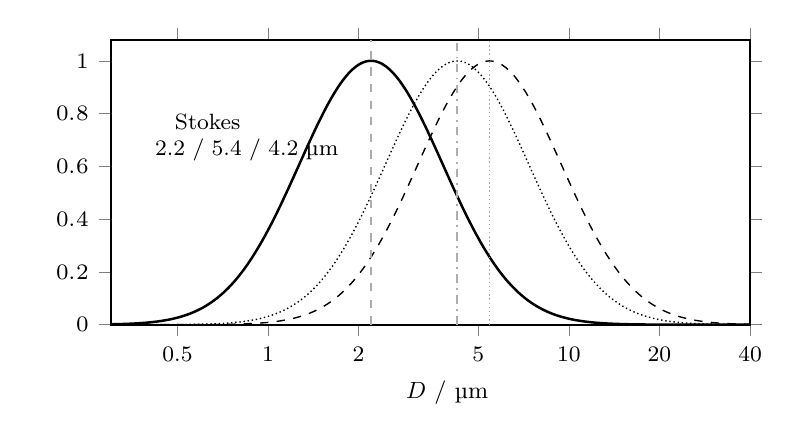
\begin{tikzpicture}
\begin{axis}[
  width=\onecolwidth, height=52mm,
  xmode=log, log basis x=10,
  xmin=0.3, xmax=40, ymin=0, ymax=1.08,
  domain=0.3:40, samples=400,
  xtick={0.5,1,2,5,10,20,40}, xticklabels={0.5,1,2,5,10,20,40},
  ytick={0,0.2,0.4,0.6,0.8,1.0},
  xlabel={等效直径 $D$ / µm},
  ylabel={归一化频率},
  tick label style={font=\fontsize{8}{9.5}\selectfont},
  label style={font=\fontsize{8.5}{10}\selectfont}]
% 个数基准：对数正态，ln D 的众数为 ln 2.2、几何标准差 exp(0.55)
\addplot[domain=0.3:40,samples=400,mainline,black]
  {exp(-((ln(x)-0.788)^2)/(2*(0.55^2)))};
% 体积（质量）基准：同批颗粒按 D^3 加权，峰移到 exp(0.788+3*0.55^2)=5.45 µm
\addplot[domain=0.3:40,samples=400,thinline,black,dashed]
  {exp(-((ln(x)-0.788)^2)/(2*(0.55^2)))*(x^3)/41.5};
% 沉降法：同一批颗粒，Stokes 径 d_St = 0.78 d_V（形状因子 0.78）
\addplot[domain=0.3:40,samples=400,thinline,black,densely dotted]
  {exp(-((ln(x/0.78)-0.788)^2)/(2*(0.55^2)))*((x/0.78)^3)/41.5};
\draw[accentsoft,dashed,thinline] (axis cs:2.2,0) -- (axis cs:2.2,1.08);
\draw[accentsoft,dashdotted,thinline] (axis cs:4.25,0) -- (axis cs:4.25,1.08);
\draw[accentsoft,densely dotted,thinline] (axis cs:5.45,0) -- (axis cs:5.45,1.08);
\node[anchor=north west,font=\fontsize{8}{9.6}\selectfont,align=left,
      text width=36mm] at (axis cs:0.32,0.98)
  {实线 图像法（个数基准）\\虚线 体积基准（同批换算）\\点线 沉降法 Stokes 径\\中位径 2.2 / 5.4 / 4.2 µm};
\end{axis}
\end{tikzpicture}
\caption{同一批颗粒、三种等效口径给出的三条分布曲线。读者应看三处：\textbf{峰的位置}
（个数基准峰在约 $\qty{2.2}{µm}$，同一批颗粒换算到体积基准后峰移到约 $\qty{5.4}{µm}$；
沉降法用 Stokes 径作横轴时峰落在约 $\qty{4.2}{µm}$）；\textbf{形状与宽度的变化}（体积基准
曲线相对个数基准明显右移并变窄，这是 $d^{3}$ 加权把大颗粒的权重放大所致，不是样品变了）；
\textbf{三条竖直参考线}（分别对应三种口径下的中位径，跨度为 2.2—5.4 µm，相差约 2.5 倍）。
三条曲线各自归一到峰值 1，因此\textbf{只能比较峰的位置，不能比较峰的绝对高度}。本图为按
对数正态个数分布及其 $d^{3}$ 加权换算构造的模型曲线（横轴为等效直径 $D$，形状因子取
0.78），用来说明「同一批颗粒换一种等效定义就换一个数」，不代表任何具体样品的实测数据。
\modelmark
\figsrc{据 S1（上册）§1.2.3 2)3)，书内 p.62--64 / PDF p.81--83 所述等效粒径与分布基准
的差异计算绘制。}}
\label{fig:ch01c-equivalent}
\end{figure}

\begin{obs}
在图~\ref{fig:ch01c-equivalent} 上逐项读数：实线（图像法个数基准）的峰在横轴
$\qty{2.2}{µm}$ 处，峰高 1；虚线（同一批颗粒按体积加权）的峰在约 $\qty{5.4}{µm}$ 处，
峰高 1；点线（沉降法，横轴为 Stokes 径）的峰在约 $\qty{4.2}{µm}$ 处，峰高 1。三条竖直
参考线分别落在 $\qty{2.2}{µm}$、$\qty{4.25}{µm}$、$\qty{5.45}{µm}$。虚线与点线的形状
相同，只是整体沿横轴平移了 $\lg(1/0.78)\approx0.11$ 个数量级；实线则明显更宽、更靠左。
三者在横轴 0.3—1 µm 区间都趋近于零；虚线与点线在 15 µm 以上也已趋近于零。
\end{obs}

\begin{infer}
由上述读数只能推出下面四条，其余不能推。

（1）\textbf{「同一批颗粒」的中位径可以是 2.2 µm，也可以是 5.4 µm}——差别不来自样品，
而来自「按什么加权」。若报告只写「平均粒径 2.2 µm」而不写基准，读者无法判断这是个数中位
径还是体积中位径，两个数相差 2.5 倍。

（2）虚线与点线形状完全一致、只差一个尺度因子 0.78，说明这一处的差别\textbf{不是分布
形状的差别，而是横轴定义（等效直径口径）的差别}：同一批颗粒，用沉降法量出的「直径」系统
性地比体积等效径小。这正是「Stokes 径与几何学等效粒径不可互比」的图形表达。

（3）三条竖线给出的是三个可比性完全不同的数：2.2 µm（个数基准）、5.4 µm（体积基准）、
4.2 µm（Stokes 径）。若把它们并列写进同一张表当作「同一批样品在三种仪器上的粒径」，读者
无从区分是样品不同还是方法不同——这是粒度数据最常被误用的一种方式。

（4）本图不能用来推断任何真实样品：0.78 这个形状因子是模型设定值，不是普适换算系数；
曲线之所以光滑，是因为它由解析函数生成。真实样品的差别还叠加了团聚、形状分布与仪器
响应函数的影响。\modelmark
\end{infer}

\begin{dataflow}
\textbf{从仪器信号到可报告的粒径数。}（1）\textbf{原始量}：筛分法得到各级筛上、筛下的
\textbf{质量}；沉降法得到不同时刻的\textbf{浓度或光强}；电阻法得到\textbf{电位脉冲}的
幅度与计数；激光散射法得到各角度的\textbf{散射光强}；图像法得到每个颗粒的\textbf{投影
轮廓}。（2）\textbf{换算}：用各自的理论把原始量转为某一等效直径的粒径分级数据——沉降法
用式~\eqref{eq:ch01c-dt-g} 或式~\eqref{eq:ch01c-dt-c} 把时间换算成 Stokes 径，电阻法用
脉冲幅度换算成体积等效径，激光散射用 Fraunhofer 或 Mie 理论反演成散射等效径。
（3）\textbf{加权}：得到的是某一\textbf{基准}的分布（筛分与沉降是质量基准，图像与电阻
可给个数基准，激光散射给体积基准）。（4）\textbf{求特征值}：用
式~\eqref{eq:ch01c-dpq} 计算所需平均径，或直接读取 $D_{50}$、$D_{10}$、$D_{90}$、$D_{97}$
与最频值。（5）\textbf{报告}：必须连同等效粒径定义、分布基准、方法名与主要条件一起给出。
任何一步跳过，第（5）步的数字就不可复核。\src{S1 §1.2.3 2)3)，书内 p.62--64 /
PDF p.81--83}
\end{dataflow}

\begin{pitfall}
\textbf{误判一：把不同方法（或不同基准）的粒径直接比较。}图像法个数基准
$\qty{2.2}{µm}$ 与激光散射体积基准 $\qty{5.4}{µm}$ 是同一批样品的两个不同等效量，比大小
没有意义；「换了一台仪器，粒径涨了一倍」通常只是基准或口径变了。判据：两个数值要能比较，
必须\textbf{等效粒径定义与百分数基准都相同}，且方法原理在样品的形状与分布宽度下成立。

\textbf{误判二：用单一平均径代替分布。}$D_{50}$ 只说「一半颗粒比它小」。宽分布样品中，
$D[3,2]$ 与 $D[4,3]$ 可以相差数倍，两者对应的是完全不同的物理量（前者关联比表面积与
传质，后者被大颗粒支配）。只报一个「平均粒径」而不报跨度，无法判断样品是否均匀。

\textbf{误判三：忽略量程与假设的越界使用。}筛分法下限 38 µm，报出更细的筛分径必然是外推；
沉降法在 $Re>2$ 或 $d<0.5$~µm 时给出的 Stokes 径不成立；库尔特法不宜测多孔颗粒；X 射线
线宽化给出的是晶粒（一次颗粒）尺寸，把它当作「催化剂颗粒度」是最常见的张冠李戴。

\textbf{误判四：取样与制样不代表整体。}颗粒样品粒子数量庞大而且很不均匀，实践表明，
粒度分析时\textbf{由采样和制样分散步骤带来的误差往往比分析的测定误差更大}。大颗粒体系的
主要误差来源是采样不均匀；纳米级细微颗粒的关键是分散（团聚体会被当成一个大颗粒，从而使
分布整体右移）。所有粒度分析方法都要求颗粒之间不能相互干扰。工业催化剂床层的上段与下段
经历过的磨损、破碎与积炭不同，取样位置必须写明。
\src{S1 §1.2.3 3)，书内 p.65、p.67 / PDF p.84、p.86}
\end{pitfall}

\begin{crosscheck}
\textbf{三条互补回查。}（1）\textbf{量级互查}：由氮吸附比表面积算出的表面积等效径
$D=6/(S\rho)$ 与图像法、沉降法的数值只能比较\textbf{数量级}，不能比较具体数值——三者的
等效定义不同；若相差超过一个数量级，应先怀疑某一个测错了（如 BET 面积含微孔、图像法把
团聚体当成单个颗粒）。（2）\textbf{分布互查}：同一样品用体积基准与个数基准各测一次，
两组数据之间应该满足 $d^{3}$ 加权的换算关系；若换算后峰位对不上，说明其中一次测量有团聚
或分割（sieve 堵塞、孔管堵塞）造成的假峰。（3）\textbf{与制备记录回查}：催化剂成型前后的
粒径变化应与成型工艺一致；二次颗粒的粒径若与一次颗粒（XRD 晶粒尺寸）相差不到两倍，通常
说明样品已经严重团聚或 XRD 峰宽主要来自微应变而非尺寸。
\src{S1 §1.2.3 2)3)7)，书内 p.62--64、p.75 / PDF p.81--83、p.94}
\end{crosscheck}

\subsection{密度的三种定义与测定}

\begin{probout}
\textbf{本节回答}：同一批多孔催化剂为什么会有三个（甚至更多）都叫「密度」的数；每一个数
究竟用哪一份体积做分母；它们各自怎么测；以及如何用它们算出孔隙率与床层空隙率。

\textbf{输出}：\textbf{骨架密度}（真密度）、\textbf{颗粒密度}、\textbf{堆积密度}三个数，
以及由它们派生的\textbf{孔隙率} $p$、\textbf{空隙率} $\varepsilon$ 与\textbf{比孔容}
$v_{\mathrm{p}}$。

\textbf{本节核心判断}：密度是物质的质量与体积之比，但对多孔固体催化剂，与其表面积一样，
其所占有的空间（体积）也因度量方法的不同而有不同的含义和量值。多孔催化剂颗粒堆积时的
\textbf{外观体积}实际包括三部分：颗粒本身的三维骨架、颗粒内部孔道、堆积时颗粒之间的空隙。
因此\textbf{以不同的体积除质量，所得密度的概念也就不同}。使用任何一个密度数值之前，必须
先问三件事：这个数\textbf{测的是哪一种}体积、用什么方法测的、样品处于什么堆积状态。文献
习惯及不同的组织和机构对固体催化剂各种密度的命名或定义并不一致，本节遵循文献主要传统并
参照 ASTM 的有关定义（ASTM D3766—08（2013）等）。
\end{probout}

\subsubsection{三种体积，三种密度}

\begin{principle}
\textbf{体积的分解。}催化剂颗粒堆积时的外观体积包括骨架、内孔与颗粒间空隙：
\begin{equation}\label{eq:ch01c-volapp}
V_{\mathrm{app}}=V_{\mathrm{void}}+V_{\mathrm{pore}}+V_{\mathrm{skel}}
\end{equation}
式中 $V_{\mathrm{app}}$ 为催化剂外观体积（堆积体积）；$V_{\mathrm{void}}$ 为堆积时颗粒之间
的空隙体积；$V_{\mathrm{pore}}$ 为颗粒内部\textbf{开孔}所占的体积；$V_{\mathrm{skel}}$ 为
固体骨架体积，包括其中\textbf{封闭孔}的体积。

\textbf{三种密度。}以不同的体积除质量即得三种密度：
\begin{equation}\label{eq:ch01c-rhoskel}
\rho_{\mathrm{skel}}=\frac{m}{V_{\mathrm{skel}}}
\end{equation}
\begin{equation}\label{eq:ch01c-rhopart}
\rho_{\mathrm{part}}=\frac{m}{V_{\mathrm{pore}}+V_{\mathrm{skel}}}
\end{equation}
\begin{equation}\label{eq:ch01c-rhobulk}
\rho_{\mathrm{bulk}}=\frac{m}{V_{\mathrm{app}}}
\end{equation}
既然分母满足 $V_{\mathrm{skel}}<V_{\mathrm{pore}}+V_{\mathrm{skel}}<V_{\mathrm{app}}$，
必有
\begin{equation}\label{eq:ch01c-order}
\rho_{\mathrm{skel}}>\rho_{\mathrm{part}}>\rho_{\mathrm{bulk}}
\end{equation}
\textbf{这个不等式是一个免费的自检工具}：任何报告如果违反它，必有一项测错或命名用错。

\textbf{两个派生量。}由骨架密度与颗粒密度可求得催化剂颗粒的\textbf{孔隙率}
（porosity）$p$：
\begin{equation}\label{eq:ch01c-poros}
p=\frac{V_{\mathrm{pore}}}{V_{\mathrm{pore}}+V_{\mathrm{skel}}}
 =1-\frac{\rho_{\mathrm{part}}}{\rho_{\mathrm{skel}}}
\end{equation}
由颗粒密度与堆积密度可求得催化剂堆积的\textbf{空隙分数}（空隙率，void fraction）
$\varepsilon$：
\begin{equation}\label{eq:ch01c-voidfrac}
\varepsilon=1-\frac{\rho_{\mathrm{bulk}}}{\rho_{\mathrm{part}}}
\end{equation}
\textbf{两式的分母不同，不可混用}：$p$ 描述的是\textbf{一颗颗粒内部}的开孔占颗粒体积的
分数，是材料的孔性；$\varepsilon$ 描述的是\textbf{床层}里颗粒与颗粒之间的空隙占外观体积
的分数，是装填状态的性质。同一种催化剂，$p$ 由制备决定，$\varepsilon$ 由装填方式决定。
两个分数的乘积才是开孔占床层外观体积的总分数。

\textbf{命名混乱提示。}英国标准协会（BSI）把\textbf{包含封闭孔}的骨架体积称为表观颗粒
体积（apparent particle volume），对应的密度称为表观颗粒密度；把\textbf{排除封闭孔}的
骨架体积称为真体积（true volume）或绝对粉末体积，对应的密度称为真密度或绝对粉末密度。
但在文献中，真密度与骨架密度常被当作同义词混用。\textbf{读文献数值时，若作者没有说明
封闭孔怎么处理，这个数就有约几个百分点的系统不确定度。}

\textbf{理论密度。}$\rho$ 还有一个更根本的定义：理论密度是指在原子水平上密堆积的、不含
任何孔与缺陷的颗粒的总质量与颗粒体积总和之比。但实际的固体催化剂往往是无定形的多种物质
的不均匀混合体，因此\textbf{理论密度这一概念对固体催化剂而言并没有多少实际意义}——它
只在讨论已知结构的纯晶相（如分子筛骨架）时才有确定值。

\textbf{包裹体积。}ASTM 引入了包裹体积（envelope volume）和包裹密度的概念来表征单个颗粒
的体积和密度：包裹体积就是假想在颗粒表面紧密包覆一层膜、膜内包容的体积。显然包裹体积
包含了颗粒的骨架体积和内孔体积，但由于表面的粗糙性，这一假想膜随观测尺度的不同而变化，
膜内也包覆了颗粒外表面的一些粗糙空隙。虽然包裹体积这一概念更接近实际，但从理论上它
\textbf{大于}本处所述的「颗粒体积」。\src{S1 §1.2.4，书内 p.75--77 / PDF p.94--96}
\end{principle}

\begin{figure}[htbp]
\centering
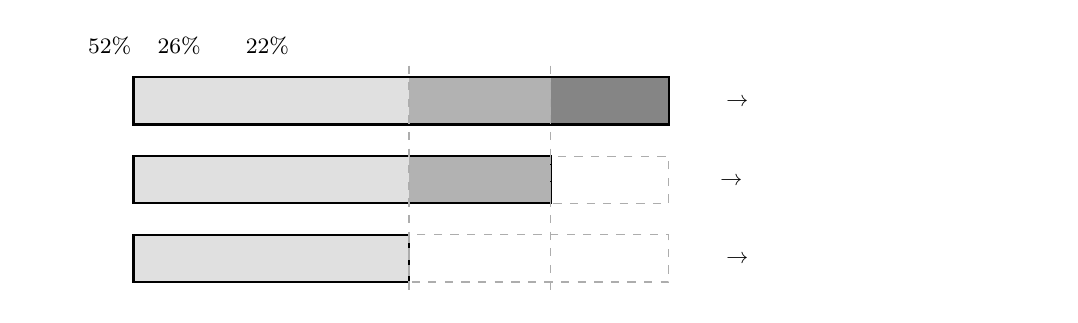
\begin{tikzpicture}[x=1mm,y=1mm]
% 比例说明
\node[anchor=west,font=\fontsize{8}{9.6}\selectfont] at (0,4)
  {示意比例：骨架 52\%、内孔 26\%、颗粒间空隙 22\%（按体积）};
% 三根条：堆积体积 / 颗粒体积 / 骨架体积
\fill[black!12]  (13.5,0) rectangle (48.5,-6);
\fill[black!30]  (48.5,0) rectangle (66.5,-6);
\fill[black!48]  (66.5,0) rectangle (81.5,-6);
\draw[thick] (13.5,0) rectangle (81.5,-6);
\fill[black!12]  (13.5,-10) rectangle (48.5,-16);
\fill[black!30]  (48.5,-10) rectangle (66.5,-16);
\draw[thick] (13.5,-10) rectangle (66.5,-16);
\draw[dashed,accentsoft] (66.5,-10) rectangle (81.5,-16);
\fill[black!12]  (13.5,-20) rectangle (48.5,-26);
\draw[thick] (13.5,-20) rectangle (48.5,-26);
\draw[dashed,accentsoft] (48.5,-20) rectangle (81.5,-26);
% 段内标签
\node[font=\fontsize{8}{9.6}\selectfont] at (31,-3)   {骨架};
\node[font=\fontsize{8}{9.6}\selectfont] at (57.5,-3) {内孔};
\node[font=\fontsize{8}{9.6}\selectfont] at (74,-3)   {空隙};
% 左侧标签
\node[anchor=west,font=\fontsize{8}{9.6}\selectfont] at (0,-3)  {堆积体积};
\node[anchor=west,font=\fontsize{8}{9.6}\selectfont] at (0,-13) {颗粒体积};
\node[anchor=west,font=\fontsize{8}{9.6}\selectfont] at (0,-23) {骨架体积};
% 右侧标签
\node[anchor=west,font=\fontsize{8}{9.6}\selectfont,align=left,text width=44mm] at (83.5,-3)
  {外观体积 $\rightarrow$ 堆积密度（含颗粒间空隙与内孔）};
\node[anchor=west,font=\fontsize{8}{9.6}\selectfont,align=left,text width=44mm] at (83.5,-13)
  {含内孔 $\rightarrow$ 颗粒密度（压汞法）};
\node[anchor=west,font=\fontsize{8}{9.6}\selectfont,align=left,text width=44mm] at (83.5,-23)
  {只含骨架 $\rightarrow$ 骨架密度（真密度）};
% 竖直参考线
\draw[dashed,accentsoft] (48.5,1.5) -- (48.5,-27.5);
\draw[dashed,accentsoft] (66.5,1.5) -- (66.5,-27.5);
\end{tikzpicture}
\caption{三种密度各自的分母是哪一份体积。读者应看\textbf{三根条的长度}：堆积体积最长
（骨架＋内孔＋颗粒间空隙），颗粒体积少了颗粒间空隙，骨架体积只剩固体本身；竖直虚线标出
三者的分界。由此可直接读出三种密度的定义式（式~\eqref{eq:ch01c-rhoskel}—
式~\eqref{eq:ch01c-rhobulk}）：\textbf{分子相同，分母依次变小，所以数值依次变大}。
示意图中的体积比例（骨架 52\%、内孔 26\%、空隙 22\%）只是为了让三段都看得见，不代表某种
具体催化剂的实测值；实际催化剂的内孔与空隙比例随制备与装填方式变化很大。\schemamark
\figsrc{据 S1（上册）§1.2.4，书内 p.75--76 / PDF p.94--95 的体积分解关系绘制。}}
\label{fig:ch01c-volume}
\end{figure}

\subsubsection{骨架密度（真密度）的测定}

骨架体积是催化剂颗粒固体骨架及其中包含的封闭孔的体积（此处参考了 ASTM 的定义）。它的
测定基于\textbf{阿基米德原理}：将一定质量 $m$ 的多孔颗粒（粉末）浸入可润湿的液体或气体
介质中，当润湿性介质完全进入颗粒的间隙和颗粒内的开孔后，颗粒置换出的介质体积即为颗粒的
骨架体积 $V_{\mathrm{skel}}$，于是 $\rho_{\mathrm{skel}}=m/V_{\mathrm{skel}}$。

测定方法有氦比重计法和比重瓶法两种。

（1）\textbf{氦比重计法}（helium pycnometry）以氦气作置换介质。将颗粒样品置于样品池中，
充高纯氦气至一定压力，然后连通参考池使氦气膨胀。样品池和参考池的体积已知，记录温度和两个
过程的平衡压力，根据\textbf{质量守恒}确定样品的体积，计算出骨架密度。氦分子小、惰性且不
被吸附，能进入绝大多数开孔；对氦气能渗透进去的材料，也可改用氮气或 \ce{SF6}。许多商品化
的全自动骨架密度计测量原理即基于氦比重计法。

（2）\textbf{比重瓶法}（specific gravity bottle method）在 Gay-Lussac 比重瓶中放置适量
的颗粒样品，通过差重法称量样品的质量及其置换出水的质量，计算骨架密度。比重瓶法设备简单、
精确度高，但操作略显烦琐。除水以外，还可以采用其他与试样润湿但不反应的液体介质（如煤油、
苯等）。\textbf{所测样品必须严格干燥；实验时样品须完全润湿并注意除气}——残留在孔内的
气泡会使置换体积偏小，从而把骨架密度算大。

至于「封闭孔算不算进骨架体积」，请回看 §1.2.4 的命名提示：含封闭孔的叫骨架密度（BSI 的
表观颗粒密度），排除封闭孔的叫真密度（BSI 的绝对粉末密度）。两种口径的差别就是封闭孔的
体积分数，对高封闭孔含量的样品可以到百分之几。\src{S1 §1.2.4 2)，书内 p.75--76 /
PDF p.94--95}

\subsubsection{颗粒密度的测定}

颗粒体积由颗粒内的孔体积 $V_{\mathrm{pore}}$ 和颗粒骨架体积 $V_{\mathrm{skel}}$ 两部分
组成，$\rho_{\mathrm{part}}=m/(V_{\mathrm{pore}}+V_{\mathrm{skel}})$。常压下，
\textbf{汞只能充填颗粒之间的间隙而不能侵入颗粒内部孔}，故可用\textbf{压汞法}测得颗粒体积，
求算颗粒密度；压汞法测得的颗粒密度也称\textbf{汞置换密度}。这里必须强调一句使用方法上的
话：\textbf{该值的大小与压汞法使用的压力有关}——压力升高后汞开始侵入较大的孔，被计入
「颗粒体积」的孔就减少，密度随之变大。因此报出汞置换密度时必须同时报出所用压力（或压力
上限）。

商品化的\textbf{包裹密度分析仪}采用另一种置换介质：用高流动性、均匀刚性的固体微球包覆所测
颗粒样品的外表面，并填充颗粒间隙空间（类似于代替了压汞法的置换介质汞），由此测定包裹密度。
包裹体积包含了骨架体积与内孔体积，由于表面粗糙性还会包住一部分外表面的粗糙空隙，所以
包裹密度略小于本处定义的颗粒密度。

本处使用的「颗粒密度」概念等同于 BSI 使用的「有效颗粒密度」（effective particle density）；
BSI 也有类似于 ASTM 的包裹体积与包裹密度概念。\src{S1 §1.2.4 3)，书内 p.76--77 /
PDF p.95--96}

\subsubsection{堆积密度的测定}

堆积密度定义为质量除以颗粒的堆积体积，堆积体积是一种\textbf{外观体积}（apparent volume），
$\rho_{\mathrm{bulk}}=m/V_{\mathrm{app}}$，因此堆积密度又称外观密度。它与颗粒的形状、装填
的方式及容器的形状有关。采用标准化的装填和测定方法或者仪器可以得到重复性很好的颗粒堆积
密度。依据测定方法的不同，堆积密度也有多种分类，如\textbf{振实堆积密度}、\textbf{松装堆积
密度}、\textbf{振动堆积密度}（vibrational packing density，ASTM）和\textbf{体积密度}
（bulk density）。测堆积密度的标准方法有 GB/T 6286—1986《分子筛堆积密度测定方法》、
ASTM D4180—13、ASTM D6683—14 等。

同样的命名分歧也出现在这里：ASTM D3766—05（2013）也使用体积密度（bulk density）一词表示
堆积密度；BSI 使用表观粉末密度（apparent powder density）；tapped density 和
tap density 也各有自己的定义。商品化仪器测定堆积密度时并不使用完全相同的标准，
\textbf{使用数据时必须注意是哪一个标准、哪一种装填方式}。

在工业生产实践中，固定床反应器催化剂装填还有\textbf{袋式装填密度}（sock loading density）
和\textbf{密相装填密度}（dense loading density）之分，它们是特定催化剂装填方式下工业催化剂
在反应器内的堆积密度：

\begin{itemize}
\item \textbf{袋式装填法}是通过一个接在催化剂料斗出口的帆布筒，靠自然重力直接把催化剂倒入
反应器的简单装填方法。适用于催化剂易积炭、床层易堵塞的反应过程。缺点是催化剂装填得不是很
均匀，容易产生沟流和热点。
\item \textbf{密相装填}是利用专门的装填器，通过空气推进或动能推进的方式将催化剂条均匀地
水平分散在催化剂床层截面。密相装填有效地避免了因催化剂条架桥造成的床层空隙，能够强化传质，
降低返混与沟流。\textbf{密相装填密度一般比袋式装填密度大 10\%—15\%}。
\end{itemize}

这 10\%—15\% 不是测量误差，而是\textbf{同一个床层里真实存在的差别}：它同时改变床层的
持气量、压降与停留时间分布。在反应器设计中把实验室松装密度直接用作工业装填密度，是
装填量算错、热点位置预测错误的常见原因。\src{S1 §1.2.4 4)，书内 p.77--78 /
PDF p.96--97}

\begin{table}[htbp]
\centering
\caption{三种密度：定义、测定方法、典型值与常见误用。读者应重点看第二列与第四列：
第二列决定这个数\textbf{测的是哪一种体积}，第四列是把它用错时最常出现的方式。
\supp{「典型值」一列为数量级参考（以 γ-氧化铝基载体与条状催化剂为例），不是原书数据；
具体数值随制备与成型工艺变化很大。}\src{原书无此汇总表，据 S1 §1.2.4，书内 p.75—78 /
PDF p.94—97 归纳。表中「典型值」一列及「常见误用」列为改编本归纳与教学设定，非源书实验数据。}}
\label{tab:ch01c-density}
{\srcsize
\begin{tabularx}{\columnwidth}{@{}lXXXX@{}}
\toprule
名称（文献别名） & 计入的体积（分母） & 测定方法与依据标准 & 典型数量级 & 常见误用 \\
\midrule
骨架密度（真密度；BSI：表观颗粒密度／绝对粉末密度） &
固体骨架体积 $V_{\mathrm{skel}}$，\textbf{含封闭孔}；排除封闭孔的口径称真体积 &
氦比重计法（气体膨胀、质量守恒）；比重瓶法（阿基米德原理，介质为水、煤油、苯等）。样品须严格干燥、完全润湿并除气 &
约 $3.0$--$3.2$ $\mathrm{g\,cm^{-3}}$ &
把「含封闭孔」与「排除封闭孔」两种口径混为一谈；把 XRD 精修得到的晶胞密度（理论密度）当作骨架密度 \\
颗粒密度（汞置换密度；BSI：有效颗粒密度） &
$V_{\mathrm{pore}}+V_{\mathrm{skel}}$，即骨架＋颗粒内\textbf{开孔} &
压汞法：常压下汞只充填颗粒间空隙、不侵入内孔；包裹密度分析仪用刚性微球填充颗粒间隙 &
约 $1.3$--$1.6$ $\mathrm{g\,cm^{-3}}$ &
把颗粒密度当作真密度使用；引用汞置换密度而不注明压汞压力（压力越高数值越大） \\
堆积密度（外观密度；体积密度；表观粉末密度） &
$V_{\mathrm{app}}=V_{\mathrm{void}}+V_{\mathrm{pore}}+V_{\mathrm{skel}}$，\textbf{含颗粒间空隙} &
标准量筒自由沉降（松装）、振实（GB/T 6286）、振动（ASTM D4180、D6683）；工业上另有袋式与密相装填密度 &
约 $0.6$--$0.8$ $\mathrm{g\,cm^{-3}}$ &
把堆密度当真密度；不写装填方式与依据标准——袋式与密相装填可相差 10\%—15\% \\
理论密度（晶胞密度） &
原子水平上密堆积、无孔无缺陷的固体体积 &
由晶体结构与晶胞参数计算，只对已知结构的纯晶相有确定值 &
随晶相而定 &
对无定形多组分催化剂使用这一概念；把它与骨架密度互换使用 \\
\bottomrule
\end{tabularx}}
\end{table}

\begin{measure}
\textbf{三个数各自的条件。}（1）\textbf{骨架密度}：样品必须严格干燥（表面水与孔内水都会
使质量偏大）、完全润湿并除气；气体置换法要记录两个平衡压力与温度；液体置换法要选与试样
润湿但不反应的介质。（2）\textbf{颗粒密度}：决定性的条件是\textbf{压力}——常压下汞只填
间隙，一旦加压到汞开始侵入孔，测到的就不再是颗粒体积；包裹密度法要说明所用微球的粒径与
流动性。（3）\textbf{堆积密度}：决定性的条件是\textbf{装填方式}（自由沉降、振实、振动、
工业袋式／密相）与容器形状；不同标准之间不可直接比较数值。
（4）\textbf{取样}：固定床催化剂的上下段、不同批次、运输前后，其堆密度与颗粒密度都可能有
系统差别，必须写明取样位置与是否经过筛分除去碎粉。\src{S1 §1.2.4，书内 p.75--78 /
PDF p.94--97}
\end{measure}

\begin{dataflow}
\textbf{从称重与压力数据到孔性判断。}（1）原始量：质量 $m$、置换出的介质体积（或氦气膨胀
前后的压力与池体积）、汞压入量与压力、量筒中的堆积体积。（2）按式~\eqref{eq:ch01c-rhoskel}
—式~\eqref{eq:ch01c-rhobulk} 得到三个密度。（3）用式~\eqref{eq:ch01c-order} 检查次序：
$\rho_{\mathrm{skel}}>\rho_{\mathrm{part}}>\rho_{\mathrm{bulk}}$ 必须成立，不成立就先
查命名与单位。（4）用式~\eqref{eq:ch01c-poros} 与式~\eqref{eq:ch01c-voidfrac} 分别算出
颗粒孔隙率 $p$ 与床层空隙率 $\varepsilon$。（5）判断：若 $p$ 明显小于由氮吸附测得的
比孔容所对应的孔隙率，说明颗粒密度测高了（多半是汞压过高，把一部分内孔算进了骨架）；
若 $\varepsilon$ 异常小，说明装填方式或碎粉含量有问题。
\src{S1 §1.2.4，书内 p.75--78 / PDF p.94--97}
\end{dataflow}

\begin{pitfall}
\textbf{误判一：把堆密度当真密度。}这是本节最高频的错误。堆密度的分母里含颗粒间空隙，
它的数值比骨架密度小好几倍；把它代入孔容、孔隙率或传质计算，会连带把后面所有的数算错。
判据：任何密度数值都必须能回答「分母里有没有颗粒间空隙」。

\textbf{误判二：把压汞法的颗粒密度当真密度。}汞置换密度含颗粒内开孔，它等于 BSI 的有效
颗粒密度，不等于骨架密度；而且它随压汞压力变化。

\textbf{误判三：不写方法与口径就引用数值。}同一名称在不同标准下定义不同（骨架密度 vs 真
密度、堆积密度 vs 体积密度 vs 表观粉末密度），文献值相差几个百分点到十几个百分点时，往往
不是样品差别而是命名差别。

\textbf{误判四：取样不代表整体。}催化剂床层上段与下段经历的温度、积炭与磨损不同，堆密度、
颗粒密度与强度都可能不同；用床层某一段的样品代表整个反应器，是工业测定的常见错误。此外，
样品若在取样时产生碎粉而未过筛，堆密度会偏大（细粉填隙）。\src{S1 §1.2.4，书内
p.75--78 / PDF p.94--97}
\end{pitfall}

\begin{crosscheck}
\textbf{四种互查，全部只用已经测过的数。}（1）\textbf{次序检查}：由
式~\eqref{eq:ch01c-order}，三个密度必须依次减小；违反次序说明命名或测量有误。
（2）\textbf{比孔容检查}：由三种密度可直接算出\textbf{比孔容}
\begin{equation}\label{eq:ch01c-vp}
v_{\mathrm{p}}=\frac{1}{\rho_{\mathrm{part}}}-\frac{1}{\rho_{\mathrm{skel}}}
\end{equation}
它应当与氮吸附法（或压汞法）测得的比孔容在允差内一致。不一致时按下面的顺序排查：先看
$v_{\mathrm{p}}$ 偏小还是偏大——偏小通常是颗粒密度测大了（压汞压力过高、或颗粒密度里
混入了封闭孔），偏大通常是骨架密度测小了（样品未完全干燥或除气不净）。
（3）\textbf{孔隙率与空隙率的量纲检查}：$0<p<1$、$0<\varepsilon<1$ 且两者互不包含；
把 $p$ 与 $\varepsilon$ 相加当作总孔率是错的。
（4）\textbf{与强度数据回查}：密相装填密度高的床层，其整体堆积抗压碎强度通常也更高
（架桥少、接触点多），若两者趋势相反，应检查装填方式或颗粒形状是否与报告一致。
\src{S1 §1.2.4，书内 p.75--78 / PDF p.94--97}
\end{crosscheck}

\subsection{催化剂机械强度的测定}

\begin{probout}
\textbf{本节回答}：催化剂的「强度」到底指什么；单颗粒强度与整体（堆积）强度为什么不能
互相替代；同一个样品为什么换一种加载方式就换一个数值；以及强度数据必须连同哪些条件报告。

\textbf{输出}：静态负荷下的\textbf{抗压碎强度}（单颗粒径向抗压碎力、点抗压碎力、整体堆积
抗压碎强度）与动态负荷下的\textbf{磨损性能}（磨耗率、磨损指数）。

\textbf{本节核心判断}：催化剂的机械强度是指其抵抗各种外界机械应力作用的能力。工业催化剂
从其生产、运输、装填直至工艺运转要经历多种应力，机械强度是判断其可靠性的重要物性技术指标
之一。为保证反应的顺利进行，主要关心的还是它\textbf{在实际工艺运转条件下}承受机械应力、
磨损和碰撞的能力。固体催化剂的工业应用主要有固定床和流化床两种形式，因而机械强度主要用
\textbf{静态负荷}和\textbf{动态负荷}测量：静态时的机械强度主要以\textbf{抗压碎强度}
表征，动态时则以\textbf{磨损性能}表征。有关测试方法大多实现了标准化，其设计原则都是尽可能
模拟催化剂在反应器内的实际工况，以保证强度数据对催化剂的应用有充分敏感性——\textbf{因此
强度数值只有在「加载方式＋试样形状＋判据」三者都相同时才可以比较}。
\end{probout}

\subsubsection{静态负荷：抗压碎强度}

\paragraph{单颗粒抗压碎强度}代表性标准有 HG/T 2782—2011《化肥催化剂颗粒抗压碎力的测定》、
HG/T 2783—1996（2010）《分子筛抗压碎力试验方法》、ASTM D4179 和 ASTM D6175—03（2013）。
单颗粒抗压碎强度测定使用颗粒强度测定仪，对处理后的催化剂样品颗粒\textbf{径向}（条形、
圆柱形样品）或者\textbf{点}（球形样品）接触施加压力，记录该颗粒被压碎时所施的力：

\begin{itemize}
\item \textbf{径向抗压碎力}：以颗粒径向方向的一个长度单位上所受的力表示，单位
$\mathrm{N\,cm^{-1}}$；
\item \textbf{点抗压碎力}：以颗粒直径方向上受的力表示，单位 N。
\end{itemize}

\textbf{单位不同就意味着物理意义不同}：径向值除以颗粒长度，反映的是条状催化剂侧壁的抗
压能力；点值不除以长度，反映的是球形颗粒整体的抗压能力。两者不能互相换算。为保证数据的
可靠性和代表性，需要测量\textbf{足够数量}的颗粒，数据以抗压碎力\textbf{均值和变异系数}
评价试样的抗压碎力及其均匀性——均值说明强度水平，变异系数说明成型质量的一致性；一批
均值合格但变异系数很大的催化剂，在床层中总有少数先碎的颗粒，而这些碎粉正是压降上升与
沟流的起点。\src{S1 §1.2.5 1)1)，书内 p.78 / PDF p.97}

\paragraph{整体堆积抗压碎强度}对固定床来讲，单颗粒强度并不能直接反映催化剂在床层中整体
破碎的情况，因而需要一种接近固定床真实情况的强度测试方法来表征催化剂的整体强度性能，即
\textbf{整体堆积抗压碎强度}；很多不规则形状的催化剂，其强度测试也只能采用这种方法。
代表性标准是 SHELL method SMS-1471，其基本方法如下：使用堆积抗压碎强度仪或自制设备，
测试的催化剂颗粒直径应不大于 6 mm；称量 $\qty{20}{cm^3}$ 处理后的催化剂样品放入一个截面
积为 $\qty{600}{mm^2}$ 的圆柱体不锈钢样品测量室；催化剂上覆盖直径 3—6 mm（因催化剂颗粒
尺寸而异）的\textbf{钢球} $\qty{5}{cm^3}$；不断增加的外力通过活塞施加到催化剂上，筛选并
称重在不同压力下压碎产生的\textbf{小于
420 µm 的粉末}（通过 ASTM 40 目标准筛）。堆积抗压强度 $P$ 定义为获得质量分数 0.5\% 的
420 µm 粉末时的压强（MPa）：

\begin{equation}\label{eq:ch01c-crush}
P=\frac{F}{A}
\end{equation}

式中 $F$ 为产生 0.5\% 粉末时施加在催化剂床上的力（N）；$A$ 为样品测量室的截面积
（$\mathrm{mm^2}$）。也可以通过绘制曲线（压碎粉末质量对压强）报告催化剂的堆积抗压强度。
此处已对照原页面图像（书内 p.79 / PDF p.98）：原书印「测试的催化剂颗粒直径应不大于
$6$ mm；称量 $20$ cm$^{3}$ 处理后的催化剂样品放入一个截面积为 $600$ mm$^{2}$ 的圆柱体
不锈钢样品测量室，催化剂上覆盖直径 $3\sim6$ mm（因催化剂颗粒的尺寸而异）的钢球
$5$ cm$^{3}$」，并明确 $P$ 以 MPa 计。原 PDF 文本层把「钢球」一类字样损伤为「钢球ｓｃ
耐」，本段据页面图像补全了钢球的直径与体积，并把此前误写的「钢制压板」改回原书的
\textbf{钢球}。\src{S1 §1.2.5 1)2)，书内 p.78--79 / PDF p.97--98}

\subsubsection{动态负荷：磨损性能}

\paragraph{磨耗率测定}磨耗率表征动态负荷条件下催化剂颗粒的抗磨损强度，代表性标准有
HG/T 2976—2011《化肥催化剂磨耗率的测定》、HG/T 3590—1999（2010）《制冷系统用分子筛
干燥剂抗磨耗性能的试验方法》及 ASTM D4058-96（2015）。其基本原理是：将经过预处理的催化剂
样品置于磨耗仪的磨耗筒（rotating drum）内，转动规定的时间，由于摩擦和磨蚀样品产生细小
碎颗粒（小于 850 µm，即通过 20 目标准筛），通过筛分称量计算磨耗率：

\begin{equation}\label{eq:ch01c-attrition}
A=\frac{m_{0}-m_{1}}{m_{0}}\times 100\%
\end{equation}

式中 $A$ 为磨耗率；$m_0$ 为磨耗前样品的质量；$m_1$ 为磨耗后样品的质量（以磨耗前后样品的
质量差为分子）。该法适用于片状、球状、挤压成型和不规则颗粒状催化剂。另外还有一种旋转管式
磨耗测试仪（rotating tube，Spence method）。

\paragraph{磨损指数测定}流化床工艺中的催化剂微球因高速气流的冲击而发生相互摩擦，磨损产生
的细粉会被气流夹带而损失。流化床催化剂的耐磨性能用\textbf{磨耗指数}（attrition index）
来表征，其测定依据 ASTM D5757—11（2017）。测定方法也称\textbf{高速空气喷射法}，适于测定
10—180 µm 的球体和不规则颗粒：将一定量的微球催化剂放入流化床磨损测定仪，利用特定流速的
喷射气流通过样品而发生磨耗，一定时间后产生的细粉（小于 20 µm 的颗粒）的质量分数即为
\textbf{空气喷射磨损指数}（air jet attrition index，AJI）。

\textbf{两个动态指标互不替代}：磨耗率用转筒的翻滚与滑动模拟固定床装卸与运转中的摩擦，
以 850 µm 为细粉界限；磨损指数用高速气流模拟流化床中的颗粒—颗粒、颗粒—器壁碰撞，以
20 µm 为细粉界限。同一个样品在两套方法下的排序可以不一致，因为它们模拟的是不同的磨损
机制（前者以表面磨损为主，后者以碎裂为主）。\src{S1 §1.2.5 2)，书内 p.79--80 /
PDF p.98--99}

\begin{table}[htbp]
\centering
\caption{四类强度测定的加载方式、结果表示与代表标准。读者应重点看第二列：
\textbf{试样形状与加载方式写在方法名里}，因而换一种加载方式就换一个数值，换一种结果表示
就不能互比。\src{原书无此类汇总表，据 S1 §1.2.5，书内 p.78—80 / PDF p.97—99 归纳。}}
\label{tab:ch01c-strength}
{\srcsize
\begin{tabularx}{\columnwidth}{@{}lXXX@{}}
\toprule
方法 & 加载方式与试样 & 结果表示 & 代表标准 \\
\midrule
单颗粒抗压碎强度 & 单颗条形／圆柱形颗粒\textbf{径向}对压，或球形颗粒\textbf{点}接触，加压至破碎 & 径向抗压碎力 $\mathrm{N\,cm^{-1}}$；点抗压碎力 N；报均值与变异系数 & HG/T 2782；HG/T 2783；ASTM D4179；ASTM D6175 \\
整体堆积抗压碎强度 & $\qty{20}{cm^3}$ 样品装入截面积 $\qty{600}{mm^2}$ 的样品室，上覆直径 $\qty{3}{mm}$--$\qty{6}{mm}$ 的钢球 $\qty{5}{cm^3}$，通过活塞逐级加压，筛出并称量 $<420$~µm 粉末 & 产生 0.5\% 质量分数粉末时的压强 $P=F/A$，MPa；或绘「压碎粉末质量—压强」曲线 & SHELL SMS-1471 \\
磨耗率（转筒法） & 预处理样品在磨耗筒中转动规定时间，由摩擦与磨蚀产生细粉 & 磨耗率 $A=(m_0-m_1)/m_0\times100\%$，细粉界限 $<850$~µm（20 目） & HG/T 2976；ASTM D4058 \\
磨损指数（空气喷射法） & 微球样品在流化床磨损仪中受特定流速喷射气流的冲击 & $\qty{5}{h}$ 试验后 $<20$~µm 细粉的质量分数（空气喷射磨损指数 AJI） & ASTM D5757 \\
\bottomrule
\end{tabularx}}
\end{table}

\emph{核对说明}：已对照原页面图像（书内 p.78—80 / PDF p.97—99，上册 §1.2.5）。四行与原文基本逐字相符，
代表标准 HG/T 2782、HG/T 2783、ASTM D4179、ASTM D6175、SHELL SMS-1471、
HG/T 2976、ASTM D4058、ASTM D5757 均见于原文。核对中改正两处：堆积强度行原写「上覆压板」，原书 p.79 为在催化剂上覆盖直径 $\qty{3}{mm}$--$\qty{6}{mm}$ 的钢球 $\qty{5}{cm^3}$；
磨损指数行原写「一定时间后」，原书 p.80 明确为 $\qty{5}{h}$ 试验。原书同节另有旋转管式磨耗测试仪（可同时测
4 个样品）与制冷系统用分子筛干燥剂标准 HG/T 3590，本表未收。


\begin{measure}
\textbf{强度数据的报告清单。}（1）\textbf{试样}：颗粒形状（球、条、片、三叶草、不规则）、
尺寸（直径与长度）、是否经过预处理（干燥、焙烧、筛除碎粉）、样品数。（2）\textbf{加载
方式}：径向还是点接触、加载速率、是否逐级加压、压板／转筒／喷射气流的规格与流速。
（3）\textbf{判据}：破碎的判定（力值突降、出现规定尺寸细粉的质量分数）与细粉界限
（420 µm、850 µm、20 µm 各不相同）。（4）\textbf{统计量}：均值＋变异系数（单颗粒）、
或压强值（堆积）。（5）\textbf{取样位置}：床层上段／中段／下段，运输前后。
缺少任何一项，强度数值都无法与其他实验室的数据比较。\src{S1 §1.2.5，书内 p.78--80 /
PDF p.97--99}
\end{measure}

\begin{dataflow}
\textbf{从力—位移曲线到一条可用的强度判据。}（1）原始量：颗粒强度仪给出压碎力（力—位移
曲线），堆积强度仪给出压强与各级细粉质量，磨耗仪给出磨耗前后的质量。（2）单颗粒：读每条
曲线的峰值（破碎力），按径向或点接触的定义换算成 $\mathrm{N\,cm^{-1}}$ 或 N，对几十颗
样品求均值与变异系数。（3）堆积：把「压碎粉末质量分数—压强」曲线读到 0.5\% 处，用
式~\eqref{eq:ch01c-crush} 换算成 MPa；曲线的\textbf{形状}本身也是信息——拐点早、斜率平
说明颗粒在低压下就大量破碎。（4）动态：用式~\eqref{eq:ch01c-attrition} 算磨耗率，或直接
读磨损指数。（5）判断：单颗粒均值高但变异系数大，与堆积强度偏低同时出现，通常意味着成型
工艺不均匀（条内密度梯度、黏结剂分布不匀），而不是原料强度不够。
\src{S1 §1.2.5，书内 p.78--80 / PDF p.97--99}
\end{dataflow}

\begin{pitfall}
\textbf{误判一：强度数据不写加载方式。}径向抗压碎力（$\mathrm{N\,cm^{-1}}$）与点抗压碎力
（N）单位不同、物理意义不同；同一个样品在两种加载方式下的数值不能换算，也不能比较大小。
引用文献强度值时，若不核对加载方式，很容易得出「国外催化剂强度高一倍」的错误结论。

\textbf{误判二：用单颗粒强度代表床层整体。}单颗粒强度不能直接反映催化剂在床层中整体破碎
的情况，这正是需要整体堆积抗压强度的原因；而不规则形状的催化剂甚至只能用堆积法。

\textbf{误判三：把磨耗率与磨损指数混为一谈。}两者模拟的是不同磨损机制、细粉界限也不同
（850 µm 与 20 µm），分别对应固定床与流化床，排序可以不一致。

\textbf{误判四：只看均值不看变异系数。}均值反映强度水平，变异系数反映均匀性；床层的
压降上升往往由少数先碎的颗粒触发。

\textbf{误判五：取样不代表整体。}催化剂床层上段与下段经历的应力、磨损和积炭不同，运输与
装填过程本身就会产生细粉；不写明取样位置的强度数据只代表来样，不代表反应器里的催化剂。
\src{S1 §1.2.5，书内 p.78--80 / PDF p.97--99}
\end{pitfall}

\begin{crosscheck}
\textbf{三类强度数据的互相回查。}（1）\textbf{单颗粒与堆积互查}：整体堆积抗压碎强度低而
单颗粒径向抗压碎力正常，通常不是颗粒本身弱，而是\textbf{床层}的问题——颗粒形状不规整、
装填不均、架桥导致应力集中。（2）\textbf{静态与动态互查}：抗压碎强度高但磨耗率也高的
样品是存在的（硬而脆）；两者同时偏低则提示成型密度不足或黏结剂失效。若这两项与堆积密度
的趋势不一致（密度高而强度低），应检查是否在成型时加入了过多润滑剂或造孔剂。
（3）\textbf{与工艺表现互查}：床层压降上升速度、细粉带出量与磨损指数、磨耗率应当同向；
若现场表现为「压降快速上升」而实验室磨耗率很低，应反过来怀疑取样位置（现场碎粉来自床层
上部或运输环节）或热态下的强度衰减（水热老化后的强度重测）。
\src{S1 §1.2.5，书内 p.78--80 / PDF p.97--99}
\end{crosscheck}

\srcnote{S1（上册）§1.2.2 3)（续）—§1.2.5，书内 p.61--80 / PDF p.80--99。本节涉及的
ASTM／HG 标准编号与仪器量程取自原书表 1--10 与正文；原 PDF 为 OCR 文本层，公式与表格数字
均按 OCR 上下文与学科标准形式重建，存疑处已在正文用「待核对」标出。}
}{}
\IfFileExists{chapters/parts/ch01-d.tex}{\input{chapters/parts/ch01-d}}{}
\IfFileExists{chapters/parts/ch01-e.tex}{\input{chapters/parts/ch01-e}}{}
}{}
\IfFileExists{chapters/ch02.tex}{% chapters/ch02.tex —— 第 2 章 透射电子显微镜
% 装配层：只负责按顺序引入各分片。分片缺失时跳过，便于增量成书。
% 分片文件：chapters/parts/ch02-{a..e}.tex

\IfFileExists{chapters/parts/ch02-a.tex}{% ================================================================
%  chapters/parts/ch02-a.tex
%  第 2 章  透射电子显微镜（分片 a）
%  源：S1（上册）第 2 章，书内 p.85—109 / PDF p.104—128
%  覆盖：2.1 透射电子显微镜简介；2.2 电子衍射和成像
% ================================================================

\chapterstart{透射电子显微镜}%
{本章导读：催化剂表征关心的是纳米乃至原子尺度的形貌、相组成与局域结构，而这些正是
透射电子显微镜（TEM）的长项。本章回答四个问题：电子束与薄样品作用后产生哪些可用的
信号、这些信号各自携带什么信息；衍射花样如何反推晶面间距与晶体取向；明场、暗场与
高分辨像的衬度分别由什么机制产生；以及一台电镜「看得到」和「看不到」的边界在哪里。
2.1 节简述仪器构成，2.2 节展开电子衍射与成像原理。}

\label{ch:02}

\subsection{透射电子显微镜简介}

\subsubsection{一台电镜做什么：三步信号转换}

\begin{probout}
透射电子显微镜的\textbf{输入}是一束能量为几十到几百千电子伏特的高能电子，
\textbf{输出}是两类图像化的数据：\textbf{电子显微像}（实空间强度分布）与
\textbf{电子衍射花样}（倒空间强度分布）。二者出自同一个物理过程——电子穿过薄样品时
被原子核与核外电子散射；差别只在于\textbf{把物镜后焦面还是把物镜像平面投影到荧光屏上}。
因此一台电镜的基本操作不是「拍照片」，而是\textbf{在两套坐标系之间切换}：像给出
形貌与尺寸，衍射给出晶体学与相。
\end{probout}

整台仪器可归为三个串联的环节：\textbf{电子源与照明系统}负责产生并调制一束方向与
束斑可控的电子；\textbf{成像系统（物镜—中间镜—投影镜）}负责把样品出射的电子波
按需要重新组合成像或衍射花样；\textbf{记录系统}把电子强度转成可定量处理的数字图像。
图~\ref{fig:tem-col} 给出这条信号链的骨架。

\begin{figure}[htbp]
\centering
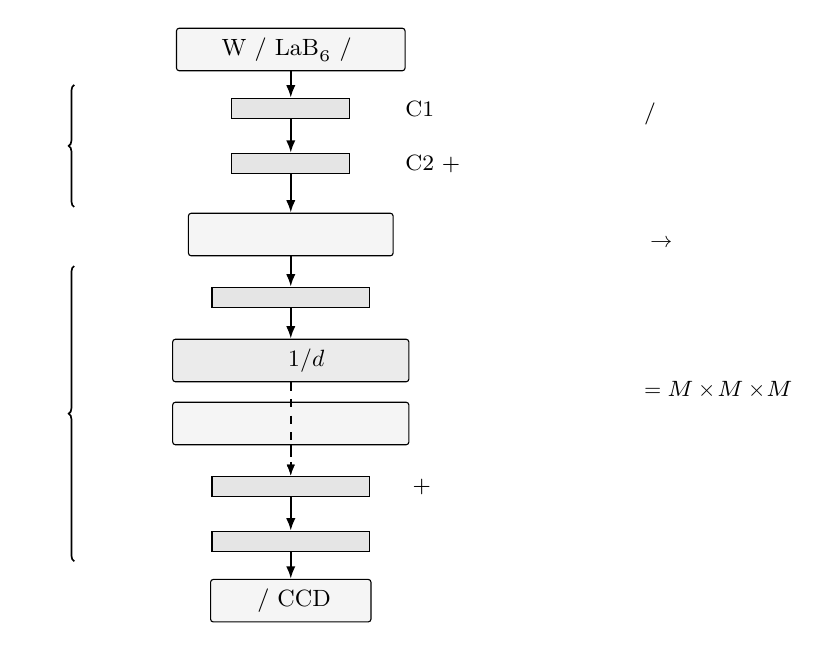
\begin{tikzpicture}[
  font=\fontsize{8}{9.5}\selectfont,
  box/.style={draw, rounded corners=1pt, minimum height=5.4mm, inner xsep=2.4mm,
              align=center, fill=black!4},
  lens/.style={draw, fill=black!10, minimum width=15mm, minimum height=2.6mm},
  ar/.style={-{Latex[length=1.6mm]}, thick},
  thin/.style={-{Latex[length=1.4mm]}, semithick, dashed}
]
% ---- 照明系统 ----
\node[box] (gun) at (0,0) {电子枪（W / LaB$_6$ / 场发射）};
\node[lens] (c1) at (0,-0.75) {};
\node[font=\fontsize{8}{9.6}\selectfont, right=0.8mm of c1] {第一聚光镜 C1};
\node[lens] (c2) at (0,-1.45) {};
\node[font=\fontsize{8}{9.6}\selectfont, right=0.8mm of c2] {第二聚光镜 C2 + 光阑};
\node[box, minimum width=26mm] (spec) at (0,-2.35) {样品（薄区，物平面）};
% ---- 成像系统 ----
\node[lens, minimum width=20mm] (obj) at (0,-3.15) {};
\node[font=\fontsize{8}{9.6}\selectfont, right=0.8mm of obj] {物镜（强磁透镜）};
\node[box, minimum width=30mm, fill=black!8] (bfo) at (0,-3.95)
      {后焦面：衍射花样（$1/d$ 坐标）};
\node[box, minimum width=30mm] (ipo) at (0,-4.75)
      {像平面：样品的放大像（实空间）};
\node[lens, minimum width=20mm] (int) at (0,-5.55) {};
\node[font=\fontsize{8}{9.6}\selectfont, right=0.8mm of int] {中间镜 + 选区光阑};
\node[lens, minimum width=20mm] (prj) at (0,-6.25) {};
\node[font=\fontsize{8}{9.6}\selectfont, right=0.8mm of prj] {投影镜};
\node[box] (scr) at (0,-7.0) {荧光屏 / CCD 相机};
% ---- 光路 ----
\draw[ar] (gun) -- (c1);
\draw[ar] (c1) -- (c2);
\draw[ar] (c2) -- (spec);
\draw[ar] (spec) -- (obj);
\draw[ar] (obj) -- (bfo);
% 【重叠修正·第二轮，2026-09-29】
% 上一轮注释声称「右移到 x=3.6 后全部让开」——**这个结论不成立**，是写在代码里的假结论。
% 实测（build/main.pdf p.16，字符级包围盒求交）仍有 4 对字形叠印，且正是同样四对。
% 真正的原因不是注记与标签相撞，而是**箭头上的 `衍射模式` 标注**：
% 这条线 (bfo) -- (int) 从 y=-3.95 到 -5.55，中点 y=-4.75 恰好落在 ipo 箱体内部
% （箱体 minimum width=30 mm，占 ±15 mm），而 right=0.6 mm 只把标注推离连线 0.6 mm，
% 仍在箱体里。实测 bbox：箱体文字 [162,489,289,497]，标注 [233,491,265,499]——标注完全落在箱体文字上。
% 修法：把标注推到箱体右外侧（15 mm 半宽 + 1.5 mm 余量）。注记在 x=36 mm，互不干涉。
% 【重叠修正·第三轮，2026-09-30】
% 上一轮注释写「把标注推到箱体右外侧（15 mm 半宽 + 1.5 mm 余量）」——**前提是错的**：
% `minimum width=30mm` 只是**最小**宽度，箱体实际宽度由文字决定。实测 ipo 箱体文字
% `像平面：样品的放大像（实空间）` 宽 127 pt，加左右 inner xsep 2.4 mm 后箱体实宽
% 49.6 mm（半宽 **24.8 mm**，不是 15 mm）。所以 right=16.5 mm 仍落在箱体里：
% 实测 p.16 上 `衍射模式` 墨迹 [278.5,302.3] 与箱体文字 [162.2,289.3] 相交 2.0×5.9 pt，
% 轮廓真实交叠 0.333 pt²。本轮按**实测箱体半宽**取 right=25 mm。
% 同理，左侧竖排标签 / 花括号原在 x=-1.18 / -0.85 cm（= -11.8 / -8.5 mm），
% 也在箱体半宽 24.8 mm 之内——`成像系统` 因此压在箱体文字上（实测 6.3×7.3 pt，
% 轮廓交叠 3.713 pt²，是全书最大的一处）。左注记列一并外移到 -3.10 / -2.75 cm。
\draw[thin] (bfo) -- node[right=25mm, font=\fontsize{8}{9.6}\selectfont]{\;衍射模式} (int);
\draw[thin] (ipo) -- (int);
\draw[ar] (int) -- (prj);
\draw[ar] (prj) -- (scr);
% ---- 右侧注记 ----
% 【重叠修正】原注记放在 x=1.35（=13.5 mm），而：镜筒节点的右挂标签从约 8.3 mm 起、
% 延伸到约 26 mm（如「第二聚光镜 C2 + 光阑」）；后焦面/像平面两个箱体 minimum width=30 mm，
% 占 ±15 mm。三处注记因此分别压在标签与箱体上（实测 p.15 出现「面/像」「实/式」「像/射」
% 「大/衍」四对字符重叠）。右移到 x=3.6（=36 mm）——但**实测该结论不成立**，
% 见下方 衍射模式 标注处的第二轮修正：真正的重叠源是箭头标注落在 ipo 箱体内部。
\node[font=\fontsize{8}{9.6}\selectfont, align=left, anchor=west] at (3.95,-0.75)
  {照明模式\\（平行束 / 会聚束）};
\node[font=\fontsize{8}{9.6}\selectfont, align=left, anchor=west] at (3.95,-2.35)
  {像的衬度在此定局：\\散射角分布 $\to$ 光阑选择};
\node[font=\fontsize{8}{9.6}\selectfont, align=left, anchor=west] at (3.95,-4.35)
  {放大倍数 $=M_{\text{物}}\!\times\!M_{\text{中}}\!\times\!M_{\text{投}}$};
\draw[decorate, decoration={brace, amplitude=2pt, mirror}, semithick]
  (-2.75,-0.45) -- (-2.75,-2.0);
\draw[decorate, decoration={brace, amplitude=2pt, mirror}, semithick]
  (-2.75,-2.75) -- (-2.75,-6.5);
\node[font=\fontsize{8}{9.6}\selectfont, rotate=90, anchor=south] at (-3.10,-1.2) {照明系统};
\node[font=\fontsize{8}{9.6}\selectfont, rotate=90, anchor=south] at (-3.10,-4.6) {成像系统};
\end{tikzpicture}
\caption{透射电子显微镜电子光学系统的信号链。读者应看两处：一是\textbf{后焦面与像平面
是两个并存的中间产物}，中间镜的物平面选谁，荧光屏上就得到衍射花样还是显微像；
二是\textbf{物镜光阑插在后焦面上}，它决定哪些散射电子能参与成像，因而决定了明场/暗场
衬度。图中高度为示意，不代表真实镜筒比例。\schemamark\figsrc{据 S1（上册）图 2-1、2-4、2-5，
书内 p.88、p.91—92 / PDF p.107、p.110—111 改绘。}}
\label{fig:tem-col}
\end{figure}

\subsubsection{部件—作用—对成像的影响}

2.1 节的逐部件叙述属可压缩内容。下表把六个部件的作用与其\textbf{对最终数据的
影响}并列，便于倒查误差来源：当一幅像出现异常时，先按「影响列」定位是哪个环节
被调错。\src{S1 §2.1.1—2.1.5，书内 p.89—93 / PDF p.108—112}

\begin{table}[htbp]
\centering
\caption{透射电镜主要部件的作用与对成像/衍射的影响}
\label{tab:tem-parts}
{\srcsize
\begin{tabularx}{\columnwidth}{@{}lXX@{}}
\toprule
部件 & 作用 & 对成像/衍射的影响（异常时的表现） \\
\midrule
电子枪 & 产生电子束，并由偏压或抽出电压调制 & 决定\textbf{相干性}：热灯丝能量分布宽、发射区大，时间与空间相干性有限；
场发射枪相干性高，信息极限高；灯丝饱和值不对则束流漂移、亮度不均 \\
照明系统（C1/C2 + 光阑） & 把电子源成像为平行束或会聚束，改变束斑大小与会聚角 & 直接改变\textbf{照射剂量}与\textbf{相干性}：缩小 C2 光阑可提高相干性
但降低剂量；会聚束/微区分析需直接调 C1 取得纳米级束斑 \\
物镜 & 在\textbf{后焦面}形成衍射花样、在\textbf{像平面}形成样品像 & 其球差系数 $C_{\mathrm{s}}$ 是点分辨率的决定因素之一；
物镜光阑决定衬度类型与最大散射角，并影响像差大小 \\
中间镜（1—2 个）+ 选区光阑 & 选择以物镜后焦面或以物镜像平面为物，从而切换衍射/成像模式 & 决定\textbf{得到的是像还是衍射}；选区光阑只在成像模式下对应确定样品区域，
光阑过小时选区与衍射实际来源区会有偏差 \\
投影镜 & 把中间镜的像/衍射进一步放大投影到屏上 & 决定最终放大倍数与视场；与中间镜一起给出总放大倍数（各透镜放大率之积） \\
记录系统（CCD 等） & 把电子强度转为数字图像 & 决定\textbf{可定量程度}：数字图像可做在线傅里叶变换、测晶格参数、监视像散；
动态范围与噪声决定了弱衬度细节能否被记录 \\
\bottomrule
\end{tabularx}}
\end{table}

\begin{principle}
磁透镜的聚焦原理：中空磁性材料极靴与其外线圈形成圆柱对称、沿轴不均匀的磁场，
运动的电子束通过时被会聚到一点。改变线圈激磁电流即改变磁场强度，从而改变
\textbf{焦距、放大倍数与聚焦状态}——电镜里没有「移动镜头」这个动作，一切调节都是
改变电流。\src{S1 §2.1，书内 p.89 / PDF p.108}
\end{principle}

\begin{pitfall}
\textbf{「放大倍数高」不等于「分辨率高」。}放大倍数是各透镜放大率之积，可以做到
$10^{6}$ 以上；而分辨率由加速电压（电子波长）与物镜球差$C_{\mathrm{s}}$ 决定，是仪器的
物理上限。把一幅低分辨率图像放大，只会把模糊一并放大。同理，换用场发射枪能提高
\textbf{信息极限}（使面间距小于点分辨率的晶格也能成像），但\textbf{不能提高点分辨率}。
\src{S1 §2.2.3，书内 p.105—108 / PDF p.124—127}
\end{pitfall}

\subsection{电子衍射和成像}

\subsubsection{电子与物质的相互作用：信号有哪几种，各来自多深}

高能电子进入固体后与原子核及核外电子发生库仑作用。按\textbf{是否损失能量}可分两类：
经过原子核静电场时只改变方向、不损失能量的称\textbf{弹性散射}；与原子电子碰撞并
把部分能量转移给它的称\textbf{非弹性散射}。二者的发生概率由各自的散射截面决定。
弹性散射截面正比于原子序数的平方，这一条是扫描透射电镜中 $Z$ 衬度像的基础。
\src{S1 §2.2.1，书内 p.94—95 / PDF p.113—114}

图~\ref{fig:tem-signals} 汇总薄样品被高能电子照射后产生的信号及其\textbf{逸出深度}。
这张图的价值在于：它同时说明了为什么 TEM 必须用薄样品（只有透射电子能穿出），
也说明了为什么同一台仪器加装谱仪后可以同时做成分分析（$X$ 射线、俄歇电子由
非弹性散射产生）。

\begin{figure}[htbp]
\centering
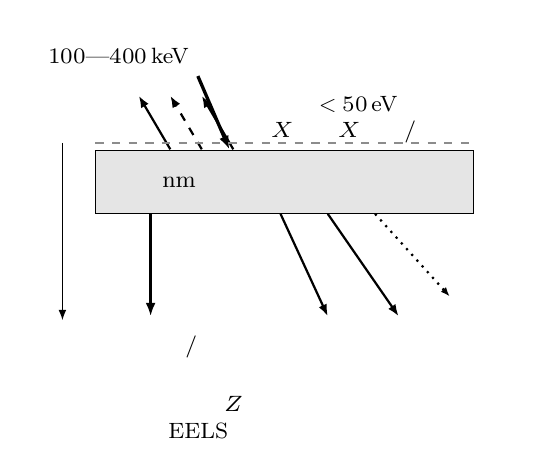
\begin{tikzpicture}[font=\fontsize{8}{9.6}\selectfont]
% 样品（薄区）
\fill[black!10] (0,0) rectangle (4.8,0.8);
\draw (0,0) rectangle (4.8,0.8);
\node[anchor=west] at (0.12,0.40) {薄样品（几十 nm）};
% 入射束
\draw[-{Latex[length=1.7mm]}, very thick] (1.30,1.75) -- (1.70,0.82);
\node[anchor=south east, align=right, font=\fontsize{8}{9.6}\selectfont]
  at (1.31,1.78) {入射高能电子\\$100$—$400$\,keV};
% 背向信号：来自表面与近表面
\draw[-{Latex[length=1.5mm]}, thick] (0.95,0.82) -- (0.55,1.50);
\draw[-{Latex[length=1.5mm]}, thick, dashed] (1.35,0.82) -- (0.95,1.50);
\draw[-{Latex[length=1.5mm]}, thick] (1.75,0.82) -- (1.35,1.50);
\node[anchor=north west, align=left, font=\fontsize{8}{9.6}\selectfont]
  at (1.85,1.62) {背散射电子、二次电子（$<50$\,eV）、俄歇电子\\
特征 $X$ 射线、连续 $X$ 射线、可见光/荧光};
% 透射信号：穿过整个样品厚度
\draw[-{Latex[length=1.7mm]}, very thick] (0.70,0) -- (0.70,-1.30);
\draw[-{Latex[length=1.5mm]}, thick] (2.35,0) -- (2.95,-1.30);
\draw[-{Latex[length=1.5mm]}, thick] (2.95,0) -- (3.85,-1.30);
\draw[-{Latex[length=1.2mm]}, thick, dotted] (3.55,0) -- (4.50,-1.05);
\node[anchor=north west, align=left, font=\fontsize{8}{9.6}\selectfont]
  at (0.15,-1.42) {未偏转透射电子（无能量/动量改变）\\与衍射电子（相干弹性散射）：};
\node[anchor=north west, align=left, font=\fontsize{8}{9.6}\selectfont]
  at (0.15,-2.05) {\textbf{晶体结构}与相的主要来源，也是高分辨像的成像\\电子。大角非相干弹性散射电子给出 $Z$ 衬度像；非弹\\性散射电子给出 EELS 信号};
% 逸出深度轴
\draw[-{Latex[length=1.3mm]}] (-0.42,0.90) -- (-0.42,-1.35);
\node[rotate=90, anchor=south, font=\fontsize{8}{9.6}\selectfont] at (-0.62,-0.30) {逸出深度（示意）};
\draw[dashed, black!45] (0,0.90) -- (4.8,0.90);
% 【重叠修正·第二轮，2026-09-30】`样品表面` 原在 (3.2,0.92)，正落在两行注记
% `背散射电子、二次电子…` / `特征 X 射线…` 的**中间**（两行基线 476.15 / 486.12，
% 本标注 481.19，各差 5.04 pt），实测 11 对字形墨迹相交（最大 `品`×`连` 1.182 pt²）。
% 改挂在样品矩形右侧、与 `薄样品（几十 nm）` 同一水平线上，避开两行注记的 x 区间。
\node[anchor=west, font=\fontsize{8}{9.6}\selectfont] at (4.90,0.40) {样品表面};
\end{tikzpicture}
\caption{高能电子与薄样品相互作用产生的信号及其来源深度。读者应看\textbf{箭头的方向}：
向上（背向）的信号只能来自表面或近表面，携带表面成分信息；向下（透射）的信号穿过
整个样品厚度，是\textbf{体相结构与晶体学}信息的载体，也是 TEM 成像与衍射实际使用的
电子。图中深度为定性示意，不代表具体数值。\schemamark\figsrc{据 S1（上册）图 2-6，
书内 p.95 / PDF p.114 改绘。}}
\label{fig:tem-signals}
\end{figure}

\begin{keycond}
\textbf{弹性散射是相干散射，非弹性散射是非相干散射}——除大角卢瑟福散射这一例外。
相干散射的电子保持原波长，因此可以相互干涉形成衍射花样与相位衬度像；
非弹性散射改变波长，只能贡献弥散背景。这条区分是理解「为什么衍射斑点能给出
晶体学信息」的前提。\src{S1 §2.2.1，书内 p.94 / PDF p.113}
\end{keycond}

\begin{pitfall}
电子对样品的\textbf{辐照损伤远大于 $X$ 射线}，原因是电子的原子散射因子比 $X$ 射线大
若干数量级。但反过来说，$X$ 射线谱仪为取得足够计数需要长得多的采集时间。因此
「电子束损伤小」和「采集快」是一对\textbf{需要权衡}的量，对电子束敏感的样品
（有机物、部分分子筛）必须靠降低剂量、减少曝光时间来解决，而不能靠提高加速电压
一概而论。\src{S1 §2.2.1，书内 p.95 / PDF p.114}
\end{pitfall}

\subsubsection{电子衍射：从衍射花样到晶体学结论}

\paragraph{衍射的几何条件}
电子波在晶体中周期排布的散射中心上发生相位相干的散射，在某些晶体学方向上相互
加强形成衍射波。三维晶体对电子的散射能力用\textbf{结构因子}
$F(hkl)$ 描述，它等于单胞中所有原子散射因子乘以相位因子之和；
衍射强度正比于结构因子模的平方：$I(hkl)\propto|F(hkl)|^{2}$。只有 $F(hkl)\neq 0$ 的
晶面才可能给出衍射束，这直接引出\textbf{消光规律}（表~\ref{tab:extinction-ch02}）。
\src{S1 §2.2.2，书内 p.96、p.99 / PDF p.115、p.118}

\paragraph{Bragg 方程}
衍射方向由 Bragg 条件给出。波长为 $\lambda$ 的电子波入射到晶面间距为 $d_{hkl}$ 的
晶面族上，入射角与反射角相等且入射线、反射线、晶面法线共面时，各晶面的散射波
相干加强：

\begin{equation}\label{eq:bragg-ch02}
n\lambda=2\,d_{hkl}\sin\theta_{hkl}
\end{equation}

其中 $n$ 为衍射级数（衍射指数），$\theta_{hkl}$ 为该晶面族的 Bragg 角，即衍射方向。
\begin{keycond}
式~\eqref{eq:bragg-ch02} 的成立条件：\textbf{（i）}样品在照射体积内具有长程有序的
周期结构（单晶或足够大的晶粒）；\textbf{（ii）}晶面取向与入射束恰好满足该角度关系；
\textbf{（iii）}散射为弹性（相干）散射，波长在散射前后不变。原子呈无序排列时
散射不遵从 Bragg 条件，出现弥散散射（非 Bragg 散射）；样品变厚时出现动力学效应，
斑点亮暗不均，更厚时出现菊池线。\src{S1 §2.2.2，书内 p.97 / PDF p.116}
\end{keycond}

\textbf{量纲检查}：$n$ 无量纲，$d_{hkl}$ 与 $\lambda$ 同为长度量纲，$\sin\theta$ 无量纲，
两端量纲一致。数量级的合理性可由一个常用极限看出：电子波长极小（$100$\,kV 下
$\lambda=\qty{0.0037}{nm}$），故 $\sin\theta=\lambda/(2d)\ll1$，$\theta$ 只有
零点几度——\textbf{电子衍射斑点只出现在极其接近平行于入射束的方向上}，这正是电子
衍射花样可近似用「零层倒易面」直接解读的原因。

对立方晶体，晶面间距与晶胞参数 $a$ 的关系为

\begin{equation}\label{eq:d-cubic}
\frac{1}{d_{hkl}}=\frac{\sqrt{h^{2}+k^{2}+l^{2}}}{a}
\end{equation}

\begin{keycond}
式~\eqref{eq:d-cubic} 仅适用于\textbf{立方}晶系。其他晶系必须用各自的晶面间距公式，
不能直接把 $\sqrt{h^{2}+k^{2}+l^{2}}$ 当作通用因子。
\tocheck{未对照原页面图像：式（2-7）的 OCR 形式被严重破坏，此处按立方晶系标准形式重建；
需核对原书是否对非立方晶系也给出了对应表达式。}
\end{keycond}

\paragraph{倒易空间与 Ewald 球}
把 Bragg 条件写成 $\sin\theta=(1/d)\big/(2/\lambda)$，其几何意义是：一个直角三角形的
对边为 $1/d$、斜边为 $2/\lambda$。对应的作图法是：\textbf{以入射波矢的起点为球心}
（该点在倒易原点 $O$ 沿入射反方向、距离 $1/\lambda$ 处），以 $1/\lambda$ 为半径作球，
\textbf{球面必过倒易原点 $O$}。凡落在球面上的倒易格点 $G$（$|G|=1/d$）都满足衍射条件，
由球心指向该格点的方向即衍射方向。这个球称为 \textbf{Ewald 反射球}。
注意「以倒易原点为球心」是错的：若球心在原点，球面就不可能过原点，
而衍射条件恰恰要求球面经过原点。
\tocheck{原书此处散文表述含混；本节按标准 Ewald 作图法改写，未对照原页面图像}
\src{S1 §2.2.2，书内 p.97—98 / PDF p.116—117}

\begin{principle}
Ewald 球作图法的实用推论：电子波长极短 $\Rightarrow$ 反射球半径 $1/\lambda$ 极大
$\Rightarrow$ 球面在倒易原点附近\textbf{近似为平面}。因此单张电子衍射花样近似等于
倒易空间中过原点的一个\textbf{零层倒易面}，斑点排布直接反映该带轴的二维周期。
换一个晶带轴就要倾转样品——倾转范围受物镜极靴尺寸限制。
\src{S1 §2.2.2，书内 p.98 / PDF p.117}
\end{principle}

\begin{table}[htbp]
\centering
\caption{几种常见晶体结构的消光规律（$F$ 为结构因子，$n$ 为整数）}
\label{tab:extinction-ch02}
{\srcsize
\begin{tabularx}{\columnwidth}{@{}lXl@{}}
\toprule
晶体类型 & 出现衍射的条件（选择关系） & 单胞格点数 \\
\midrule
简单（单斜，所有 $h,k,l$） & 无消光，任意 $h,k,l$ 均可 & 1 \\
体心立方 & $h+k+l=2n$（偶数） & 2 \\
面心立方 & $h,k,l$ 全为奇数或全为偶数 & 4 \\
密排六方 & $h+2k=3n$ 时 $l$ 必须为\textbf{偶数}；$h+2k=3n\pm1$ 时 $l$ 任意 & 2 \\
\bottomrule
\end{tabularx}}
\end{table}

消光规律与晶体学中由点阵类型导出的系统消光完全一致，因此\textbf{衍射斑点的有无本身
就是一条结构信息}：它是判断点阵类型（如区分面心立方与体心立方）的第一手依据。
自检方法：把选择关系代入几个具体指数做断言检验，例如密排六方的 $(0001)$
（$h=k=0\Rightarrow h+2k=0=3n$，而 $l=1$ 为奇数）\textbf{必须不出现}；
若某条规则允许它出现，该规则写错了。

\paragraph{另一条约束：晶带定律}
斑点的出现受结构因子控制，但斑点的\textbf{指数}还必须满足晶带定律：属于同一晶带轴
$[uvw]$ 的所有晶面 $(hkl)$ 满足正交关系

\begin{equation}\label{eq:zone-law}
uh+vk+wl=0
\end{equation}

\begin{keycond}
式~\eqref{eq:zone-law} 描述的是「同时被激发的衍射束所对应的晶面法线都垂直于
同一带轴」。它是索引衍射花样的判据：若某个斑点的指数不满足该式，说明它不属于
当前带轴，索引有误。\src{S1 §2.2.2，书内 p.99 / PDF p.118}
\end{keycond}

\paragraph{从衍射花样读晶面间距：相机常数}
得到衍射斑点或衍射环后，用下式把斑点到透射斑的距离换算为晶面间距：

\begin{equation}\label{eq:camlen}
r\,d=L\,\lambda \qquad\Longleftrightarrow\qquad r=\frac{L\lambda}{d}
\end{equation}

其中 $L$ 为相机长度，$r$ 为衍射点到透射斑点的距离，与 $1/d$ 成正比。对给定相机
长度，$L\lambda$ 为常数，称为\textbf{相机常数}。
\begin{keycond}
$L\lambda$ 必须用\textbf{已知结构的标准样品}实测标定，不能直接采用仪器标称值——
这一条是定量索引衍射花样的前提。另外，仅靠一两个 $d$ 值往往不能唯一确定结构：
很多金属体系的晶格常数非常接近（差别小于电镜的测量误差），此时\textbf{测量两个衍射
点之间的夹角}是重要的补充判据。\src{S1 §2.2.2，书内 p.101 / PDF p.120}
\end{keycond}

\textbf{量纲检查}：$r$（长度）$\times d$（长度）$=$ $L$（长度）$\times\lambda$（长度），
两端均为面积量纲，一致。

\begin{table}[htbp]
\centering
\caption{衍射花样的形态与可读出的样品信息}
\label{tab:pattern-read}
{\srcsize
% 原为 @{}lXX@{}：首列 l 吃掉自然宽度，两个 X 列被挤到低于最小内容宽度（29.8 pt overfull）。
% 改为定宽 p{24mm}，首列可折行，宽度留给 X 列。
% tabularx 无法把 X 列压到其最小内容宽度以下；实测该表最小宽度超版心 29.8 pt。
% 改为显式 p{} 列：24+36+88 = 148 mm，加列间距约 156 mm，小于版心 165 mm。
\begin{tabular}{@{}>{\raggedright\arraybackslash}p{24mm}>{\raggedright\arraybackslash}p{36mm}>{\raggedright\arraybackslash}p{88mm}@{}}
\toprule
花样形态 & 对应的样品状态 & 可读出 / 不可读出 \\
\midrule
清晰规则的斑点阵列 & 单晶或单个大晶粒 & 可读出带轴、$d$ 值、点阵类型（由消光）；
单张花样只是倒易空间的一个截面，确定单胞需多个带轴 \\
连续同心圆环 & 大量随机取向的小晶粒（多晶） & 各环半径给出全部可激发晶面的 $d$ 值；
环的\textbf{宽度}反映晶粒尺寸（纳米颗粒环变宽） \\
不连续/部分弧状环 & 晶粒数有限或存在择优取向（织构） & 择优取向对应的斑点特别亮；
可判断织构方向 \\
弥散晕环 & 非晶（玻璃、液体） & 环径对应原子平均间距，只反映\textbf{近程有序}；
不能给出指数与晶胞参数 \\
斑点形状偏离圆点 & 形貌三维受限（片状试样平行入射束、一维纳米结构） & 提示存在形状效应；
分析纳米材料时须纳入考虑 \\
\bottomrule
\end{tabular}}
\end{table}

\begin{measure}
\textbf{衍射花样的两条常规检查}：\textbf{（i）} 先核对 $L\lambda$ 标定是否在有效期内、
是否用与本次相同的相机长度；\textbf{（ii）} 索引后的斑点集合必须整体满足晶带定律
\eqref{eq:zone-law} 与对应晶系的消光规律，\textbf{不允许逐点凑指数}。若只挑出少数
斑点匹配而其余斑点无法解释，正确的做法是承认该花样对应多套衍射的叠加（多相共存），
而不是继续调整指数。
\end{measure}

\subsubsection{成像：三种衬度来源}

把物镜像平面投影到荧光屏上即得放大像。人眼看到的是强度分布，而不同区域或细节的
强度差异称为\textbf{像衬度}。电子波穿过样品后振幅与相位都可能改变，两类变化都能
产生衬度，据此分为\textbf{振幅衬度}（含质厚衬度与衍射衬度）和\textbf{相位衬度}。
一张照片中两种衬度可能同时存在，但总有一种占主导。表~\ref{tab:contrast} 对比三者。
\src{S1 §2.2.3，书内 p.101—106 / PDF p.120—125}

\begin{table}[htbp]
\centering
\caption{质厚衬度、衍射衬度与相位衬度的来源与适用条件}
\label{tab:contrast}
{\srcsize
\begin{tabularx}{\columnwidth}{@{}p{0.105\columnwidth}XXX@{}}
\toprule
 & 质厚衬度 & 衍射衬度 & 相位衬度（高分辨） \\
\midrule
物理来源 & 非相干卢瑟福散射；散射截面正比于样品有效质量（密度 $\times$ 厚度） &
透射束与衍射束的强度分配随晶体取向变化 & 电子波穿过晶体电势场后的相位改变，
经物镜传递函数调制后干涉成像 \\
光阑设置 & 物镜光阑居中，只让透射束通过（\textbf{明场}） &
明场：光阑居中挡掉衍射束；暗场：用衍射束成像（可偏入射束使其沿光轴通过） &
通常需两束或多束电子波相干，物镜光阑须让相应衍射束通过 \\
衬度与什么对应 & 亮 $=$ 轻元素或薄区；暗 $=$ 重元素或厚区 &
明场中满足 Bragg 条件的区域\textbf{暗}；暗场中该区域\textbf{亮} &
在弱相位近似与 Scherzer 欠焦下，衬度正比于晶体电势场的投影（暗区对应较重的原子柱） \\
最佳实验条件 & 插入物镜光阑限制散射角可提高明晰度；非晶样品唯一可用的衬度 &
需倾转样品至\textbf{双光束条件}（一个强透射束 $+$ 一个强衍射束）；
多相共存时选特定衍射束成像可分离相 & 样品必须极薄（弱相位体）、接近 Scherzer 欠焦、
厚度与取向高度敏感 \\
不适用/失效情形 & 不给出晶体学信息；不能区分同密度同厚度的不同相 &
完整等厚无缺陷晶体不产生衬度（等厚条纹、等倾轮廓线来自厚度或弯曲变化）；
纳米粒子太小、衍射束太弱，难以得到高质量暗场像 & 像衬度随欠焦量与厚度强烈变化，
不能直接一对一解释结构，须与计算模拟像比对 \\
\bottomrule
\end{tabularx}}
\end{table}

\begin{dataflow}
\textbf{一个读图实例——从衍射花样判断催化剂中的相。} 设某负载型金属催化剂的高分辨
样品给出图~\ref{fig:read-pattern} 所示的选区电子衍射花样。按下面的顺序读：
先看花样的\textbf{整体形态}，再量\textbf{环半径}，再查\textbf{消光}，最后做\textbf{交叉验证}。
\end{dataflow}

\begin{figure}[htbp]
\centering
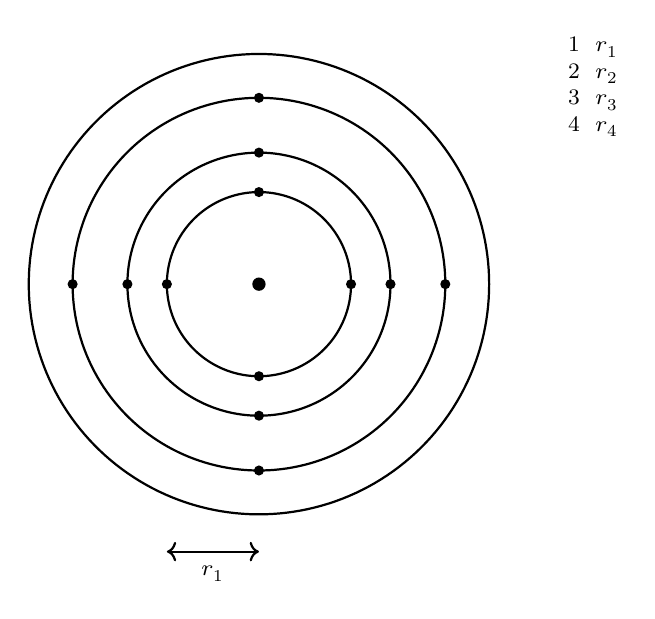
\begin{tikzpicture}[font=\fontsize{8}{9.6}\selectfont]
\begin{axis}[
  width=0.86\columnwidth, height=0.62\columnwidth,
  axis equal image, scale only axis,
  xmin=-1.35, xmax=1.35, ymin=-1.35, ymax=1.35,
  axis lines=none, clip=false,
  xtick=\empty, ytick=\empty
]
% 最强环（示意）：用参数曲线画圆
\addplot[thick, domain=0:360, samples=200, black] ({0.42*cos(x)},{0.42*sin(x)});
\addplot[thick, domain=0:360, samples=200, black] ({0.60*cos(x)},{0.60*sin(x)});
\addplot[thick, domain=0:360, samples=200, black] ({0.85*cos(x)},{0.85*sin(x)});
\addplot[thick, domain=0:360, samples=200, black] ({1.05*cos(x)},{1.05*sin(x)});
% 透射斑与少数取向偏离的强斑点（织构/大晶粒）
\addplot[only marks, mark=*, mark size=2.1pt, black] coordinates {(0,0)};
\addplot[only marks, mark=*, mark size=1.5pt, black]
  coordinates {(0.42,0) (-0.42,0) (0,0.42) (0,-0.42)
               (0.60,0) (0,0.60) (-0.60,0) (0,-0.60)
               (0.85,0) (-0.85,0) (0,0.85) (0,-0.85)};
% 标尺
\draw[<->, thick] (-0.42,-1.22) -- (0,-1.22);
\node[anchor=north, font=\fontsize{8}{9.6}\selectfont] at (-0.21,-1.24) {$r_{1}$};
\node[anchor=west, font=\fontsize{8}{9.6}\selectfont, align=left] at (1.30,0.9)
  {环 1\ \ $r_{1}$\\环 2\ \ $r_{2}$\\环 3\ \ $r_{3}$\\环 4\ \ $r_{4}$};
\end{axis}
\end{tikzpicture}
\caption{一个用于读图练习的多晶电子衍射花样示意（含少量异常明亮的斑点）。
读者应看三处：\textbf{（i）}环是连续还是断续——连续环对应随机取向的众多晶粒，
若个别斑点显著偏亮则提示存在择优取向；\textbf{（ii）}各环半径 $r_{i}$ 的比例关系，
按式~\eqref{eq:camlen} 换算成 $d$ 值之比；\textbf{（iii）}中心透射斑的位置，
它是所有 $r$ 的起点，位置没找准后面全错。本图是按衍射几何绘制的示意花样，
不是实验照片，环的强度分布不代表任何具体样品。\schemamark}
\label{fig:read-pattern}
\end{figure}

按「观察」与「推断」严格分开，读出过程如下。

\begin{obs}
\textbf{(1)} 花样由若干\textbf{连续同心环}构成，中心有一个最强斑，另有一组位于
正交点阵位置上的斑点与环重合，其亮度明显高于同半径处环的平均亮度。
\textbf{(2)} 用标定的相机常数按式~\eqref{eq:camlen} 量得前四个环的 $d$ 值，
其比例与 $1:\;0.71:\;0.61:\;0.50$ 相近。
\textbf{(3)} 前四个环之外还有若干可测环，但按 $1/d$ 排序后，前四环的\textbf{相对}
位置是确定的；本练习只对前四环做比对。
\textbf{(4)} 各环有可测宽度，且宽度随 $r$ 增大而略增。
\textbf{(5)} 该花样对应的选区（选区光阑所限区域）内，明场像中未见大块晶体，
多为 $5$—$20$\,nm 的暗色颗粒。
\end{obs}

\begin{infer}
\textbf{由 (1)}：连续环 $+$ 少量异常亮斑点 $\Rightarrow$ 样品以\textbf{随机取向的多晶}
为主，同时存在\textbf{择优取向}（或少量较大晶粒）。注意这是两个独立判断：
环的连续性说明取向随机，斑点的异常亮度说明取向分布不均匀。
\textbf{由 (2)}：把测得的 $d$ 值之比与两种立方点阵的\textbf{允许反射序列}比对
（表~\ref{tab:ring-index}）。这是读环花样的标准第一步，也是最容易出错的一步：
必须比\textbf{序列}而不只是比某一个数。

\begin{table}[htbp]
\centering
\caption{多晶环花样的指认对照（$d$ 值按第一环归一）}
\label{tab:ring-index}
{\srcsize
\begin{tabularx}{\columnwidth}{@{}llXX@{}}
\toprule
点阵 & 反射次序 & 允许反射的 $d$ 值比序列 & 与前四环 $1:0.71:0.61:0.50$ 的比对 \\
\midrule
面心立方 & 第 1—6 & $1\,(111)$、$0.87\,(200)$、$0.61\,(220)$、%
$0.52\,(311)$、$0.50\,(222)$、$0.43\,(400)$ &
第 1、3、5 项吻合，第 2、4 项不吻合 \\
体心立方 & 第 1—6 & $1\,(110)$、$0.71\,(200)$、$0.58\,(211)$、%
$0.50\,(220)$、$0.45\,(310)$、$0.41\,(222)$ &
第 1、2、4 项吻合，第 3 项差 $0.03$ \\
\bottomrule
\end{tabularx}}
\end{table}

\textbf{由表~\ref{tab:ring-index} 得出的关键判断}：观测序列 $1:0.71:0.61:0.50$
\textbf{与两种点阵都不完全吻合}——与面心立方差在第 2、4 项，与体心立方只差第 3 项
（$0.61$ 对 $0.58$，偏差约 $5\%$）。体心立方的吻合程度\textbf{明显更好}，
但偏差已接近小晶粒环宽带来的测距误差量级，因此\textbf{不能仅凭这四个数定案}。
\textbf{由 (3)}：在体心立方指认（$110$/$200$/$211$/$220$）下，$h+k+l$ 为奇数、
本应系统消光的反射（如 $111$、$311$）确实未出现在前四环中，这与体心立方相容；
但同样的相容性在面心立方指认下也成立，故 (3) 只有\textbf{排除性}价值而无\textbf{确证}价值。
\textbf{由 (4)}：环宽随 $r$ 增大提示晶粒尺寸在纳米量级并存在尺寸分布；
环宽同时是 $d$ 值测量误差的主要来源，这正是上面第 3 项 $5\%$ 偏差不能作为定案依据的原因。
\textbf{由 (5)}：样品为纳米颗粒集合体，其衍射来自大量小晶粒的叠加；
颗粒数足够多，说明「多晶」这一判断本身是稳的。
\textbf{结论（限定表述）}：该选区内存在一种\textbf{纳米晶相}，其前四环与\textbf{体心立方}
点阵的相容性优于面心立方，但两者均未被排除；$d$ 值本身\textbf{不足以}指认具体物相。
下一步必须补做：(a) 用\eqref{eq:zone-law} 晶带定律校验更完整的环序列；
(b) 多带轴单晶花样或高分辨像上量晶格条纹间距；(c) 成分分析把候选相收缩到唯一。
\end{infer}

\begin{crosscheck}
\textbf{本图的结论需要哪些外部数据回查。}
\textbf{（i）成分}：衍射只给晶体学，不给元素。与上面前四环相容的立方相候选很多
（体心立方与面心立方金属及其氧化物中都有 $d$ 值落在这个区间的相），
必须用 $X$ 射线能谱或电子能量损失谱\textbf{限定元素}，才能把「相容于某点阵」
收缩为「某个相」。
\textbf{（ii）标定}：$L\lambda$ 若未用标准样品标定，第 (2) 步的全部数值都不成立；
本例中第 3 环约 $5\%$ 的偏差恰好与标定不准确引起的系统误差同量级，
必须先排除这一项再谈点阵类型。
\textbf{（iii）选区代表性}：选区光阑越小，选区与衍射斑点真正形成的区域之间偏差越大；
选区内的颗粒数若只有几个，则「多晶」的判断本身就不稳。
\textbf{（iv）与高分辨像互证}：若能在高分辨像上量得一组晶格条纹间距并与某个环的 $d$
对应，且条纹方向与暗场像中该衍射束点亮的区域一致，则相归属的可信度显著提高。
\textbf{（v）厚度效应}：样品较厚时动力学效应会使相对强度偏离 $|F|^{2}$，
按强度比去区分相近相的做法在该厚度下不可靠。
\textbf{（vi）环宽的双重角色}：环宽既是晶粒尺寸的证据，也是 $d$ 值测量误差的来源；
用环宽论证「晶粒为纳米级」时，必须同时承认它限制了点阵判定的精度。
\end{crosscheck}

\subsubsection{高分辨相位衬度：能给出什么，什么时候不能信}

高分辨电子显微学（HRTEM）自 20 世纪 70 年代发展起来，如今商用仪器的点分辨率
普遍达到 $0.2$\,nm 或更好。它利用\textbf{相位衬度}给出点阵条纹或原子结构像——
这与低/中放大倍数下用质厚衬度和衍射衬度成像有本质区别。更准确地说，看到的高分辨像
是\textbf{电子束波相干条纹的二维投影}，像的强度是电子波干涉强度的分布，
因此不能用样品的密度或厚度直接解释，必须借助波动光学。
\src{S1 §2.2.3，书内 p.104—105 / PDF p.123—124}

\textbf{弱相位近似。} 电子穿过电势为 $V(x,y)$ 的薄样品时透射波函数为
$\psi(x,y)=\exp[\mathrm{i}\sigma V(x,y)]$，其中 $V(x,y)$ 是晶体电势场沿电子入射方向的
投影，$\sigma=\pi/(\lambda E)$ 为相互作用常数。对足够薄的样品，振幅不变而相位变化很小
（$\sigma V\ll1$，这样的样品称弱相位体），上式展开为

\begin{equation}\label{eq:weak-phase}
\psi(x,y)\approx 1+\mathrm{i}\sigma V(x,y)
\end{equation}

物镜传递函数 $A(u,v)=\exp\{\mathrm{i}\chi(u,v)\}B(u,v)D(u,v)$ 对电子波进行调制，
其中 $B$ 为束发散度引起的衰减包络函数（反映空间相干性），$D$ 为色差引起的衰减包络
函数（反映时间相干性），而 $\chi(u,v)$ 为物镜的波像差。\textbf{注意相位必须是
$2\pi$ 周期的角量}：$\chi$ 已按\textbf{弧度}定义（式中带 $\pi$ 系数），故指数上写
$\mathrm{i}\chi$；只有当 $\chi$ 被定义成\textbf{周期数}（转数）时指数才写成
$2\pi\mathrm{i}\chi$。二者混用会让整条推导与 Scherzer 条件同时错位。

\begin{equation}\label{eq:chi}
\chi(u,v)=\frac{\pi}{2}C_{\mathrm{s}}\lambda^{3}(u^{2}+v^{2})^{2}
+\pi\Delta f\,\lambda(u^{2}+v^{2})
\end{equation}

其中 $C_{\mathrm{s}}$ 为物镜球差系数，$\Delta f$ 为散焦量，$u,v$ 为空间频率。

\textbf{符号约定（最容易出错的地方）}：本式取标准约定，$\Delta f<0$ 表示\textbf{欠焦}。
此时二次项为负、四次项为正：低空间频率处 $\chi<0$，高空间频率处四次项占优使 $\chi$
转正，两者之间因此出现一段 $\sin\chi\approx-1$ 的\textbf{宽频带}——这正是 Scherzer
欠焦的用处所在。若把二次项写成 $-\pi\Delta f\lambda(u^{2}+v^{2})$，则与
$(\Delta f)_{\mathrm{Sch}}=-1.2(C_{\mathrm{s}}\lambda)^{1/2}$（负值）联立会得到两项同号、
$\chi$ 单调递增的结果，\textbf{根本不会出现}式~\eqref{eq:hrtem-contrast} 所需的宽频带。
遇到这种情况说明符号约定自相矛盾，应先统一约定再讨论成像，而不是直接引用结论。
\tocheck{原书 $\chi$ 两项的符号约定无法从 OCR 文本确定；本节按可自洽的标准约定改写}

\textbf{从出射波到像衬度。}约定傅里叶变换与逆变换为
$\tilde{f}(u,v)=\mathrm{FT}\{f\}=\iint f(x,y)\mathrm{e}^{-2\pi\mathrm{i}(ux+vy)}
\mathrm{d}x\,\mathrm{d}y$、$f=\mathrm{FT}^{-1}\{\tilde{f}\}$（因子 $2\pi$ 已含在
指数里，故 $u,v$ 是空间频率、其倒数是长度，$\chi$ 本身无量纲）。物镜把出射波按
\textbf{空间频率逐个}乘上传递函数，得到像面波
$\psi_{\mathrm{i}}=\mathrm{FT}^{-1}\{A\cdot\mathrm{FT}\{\psi\}\}$。代入
式~\eqref{eq:weak-phase} 并保留 $\sigma V$ 的\textbf{一阶项}（式~\eqref{eq:weak-phase}
给出 $\psi=1+\mathrm{i}\sigma V$，故其共轭为 $1-\mathrm{i}\sigma V$、
$|\psi|^{2}=1+\sigma^{2}V^{2}$，线性项只剩 $\mathrm{i}\sigma V$ 与 $-\mathrm{i}\sigma V$）：

\begin{equation}\label{eq:hrtem-contrast}
C(x,y)=I(x,y)-1
\approx-2\sigma\,V(x,y)\ast\mathrm{FT}^{-1}\!\left\{\sin\chi(u,v)\right\}
=-2\sigma\,\mathrm{FT}^{-1}\!\left\{\tilde{V}\sin\chi\right\}
\end{equation}

式中 $\ast$ 表示\textbf{二维卷积}。两个要点：
\textbf{（1）是卷积不是点乘。}被乘的是频谱 $\tilde{V}$，乘完还要做逆变换，等效于把
势投影 $V$ 与点扩散函数 $\mathrm{FT}^{-1}\{\sin\chi\}$ 卷积；写成
$V\cdot\mathrm{FT}\{\sin\chi\}$ 是把实空间量与被乘过的频谱当成同类量，量纲和单位都对不上。
\textbf{（2）近似丢掉了什么。}精确式在 $\sigma V$ 的一阶项之外还有
$-2\sigma^{2}\{V^{2}-[V\ast\mathrm{FT}^{-1}\{\cos\chi\}]^{2}\}$ 的二阶项；弱相位体
（$\sigma V\ll1$）下它可略，本节一律只保留一阶项。

\textbf{量纲检查}：$\chi$ 是相位，无量纲；$C_{\mathrm{s}}\lambda^{3}(u^{2}+v^{2})^{2}$
中 $C_{\mathrm{s}}$ 为长度、$\lambda$ 为长度、$u$ 为长度的倒数，故
长度$^{4}\times$长度$^{-4}$ 无量纲，与 $\Delta f\lambda(u^{2}+v^{2})$ 一致，
两项量纲相符。

\begin{keycond}
式~\eqref{eq:hrtem-contrast} 说明高分辨像衬度受\textbf{球差、光源相干性与散焦}
三者共同控制，故高分辨像\textbf{不是}结构的直接投影。只有在
$\sin\chi\equiv-1$（在关心的空间频率范围内为常量）时，
$\mathrm{FT}^{-1}\{\sin\chi\}=-\delta$，卷积退化为点乘，才有
$C(x,y)=2\sigma V(x,y)$——衬度正比于晶体势函数的投影，
像才反映真实结构。实际做法是对固定的 $C_{\mathrm{s}}$，取 Scherzer 最佳欠焦
$(\Delta f)_{\mathrm{Sch}}=-1.2\,(C_{\mathrm{s}}\lambda)^{1/2}$，使 $\sin\chi$ 在
很宽的空间频率范围内接近 $-1$。此时较暗的区域对应较重的原子柱。
\src{S1 §2.2.3，书内 p.105 / PDF p.124}
\end{keycond}

\begin{pitfall}
\textbf{晶格条纹不等于结构像。} 在远离 Scherzer 欠焦的条件下成像，即使样品非常均匀
且很薄，晶条纹像也不是晶体结构像或其二维投影。样品厚度很小的变化、样品取向的微小
改变都会强烈改变高分辨像的衬度，金属氧化物等复杂结构尤为敏感——同一晶体在不同
欠焦量与厚度下可以给出看起来完全不同的像。因此\textbf{正确解释高分辨像的唯一方法是
用已知结构计算模拟像并与实验像比对}（或系统变焦拍一系列欠焦量的图做计算处理）；
直接把晶格条纹与晶格结构对应的尝试可能导致错误结论。
\src{S1 §2.2.3，书内 p.108 / PDF p.127}
\end{pitfall}

\subsubsection{分辨率：三个不同的定义}

先看波动光学给出的分辨率定义：$R=0.61\lambda/(n_{\mathrm{r}}\sin\alpha)$，其中
$n_{\mathrm{r}}$ 为物与透镜之间介质的折射系数，$\alpha$ 为光束相对于光阑的半角；
光学显微镜的分辨极限约 $0.2$\,\textmu m。提高分辨率的手段是减小波长或增大介质折射率。
电镜中高能电子的波长远小于可见光，这是分辨率大幅提高的根本原因。
\src{S1 §2.2.3，书内 p.106 / PDF p.125}

\paragraph{电子波长与加速电压}
不计相对论效应时，电子被电势差 $U$ 加速后得到的德布罗意波长为

\begin{equation}\label{eq:lambda-nonrel}
\lambda=\frac{h}{p}=\frac{h}{\sqrt{2m_{0}eU}}
\end{equation}

加速电压 $100$\,kV 时，式~\eqref{eq:lambda-nonrel} 给出
$\lambda=\qty{0.00388}{nm}$。这里有一处\textbf{原书的不自洽需要指出}：
原书正文在该处取 $\lambda=\qty{0.0037}{nm}$，而 $0.0037$\,nm 只有\textbf{计入相对论修正}
才能得到——按式~\eqref{eq:lambda-rel} 算得 $\lambda=\qty{0.00370}{nm}$。
也就是说，原书所列的是非相对论公式，但其数值取自相对论结果。
本书\textbf{保留原式并写明该差异}，不作静默改动；使用时请以相对论值为准。
\tocheck{该差异由公式与数值的自洽性核算得出，未对照原页面图像}
但电子的加速电压已达几百千伏，速度接近光速，必须做\textbf{相对论修正}：

\begin{equation}\label{eq:lambda-rel}
\lambda=\frac{h}{\sqrt{2m_{0}eU\left(1+\dfrac{eU}{2m_{0}c^{2}}\right)}}
=\frac{h}{\sqrt{2m_{0}eU}}\left(1+\frac{eU}{2m_{0}c^{2}}\right)^{-1/2}
\end{equation}

\begin{keycond}
式~\eqref{eq:lambda-rel} 的成立条件与适用范围：适用于自由电子在真空中的加速；
$U$ 就是\textbf{加速电压（电势差）本身}，不是「修正后的电压」——相对论效应全部
体现在括号内的修正项中，不要把修正再算进 $U$。
括号内 $eU/(2m_{0}c^{2})$ 为相对论修正项：$U=100$\,kV 时 $eU\approx\qty{1e5}{eV}$、
$m_{0}c^{2}\approx\qty{511}{keV}$，修正项约 $0.098$，即约 $10\%$——在此电压下
\textbf{不可忽略}；电压越高，修正项越大。
\textbf{量纲检查}：$eU$ 为能量量纲，$m_{0}c^{2}$ 亦为能量量纲，比值无量纲；
根号内两项同为能量与质量之积的量纲，取根后与动量同量纲，$h/p$ 给出长度。一致。
\src{S1 §2.2.3，书内 p.106—107 / PDF p.125—126}
\end{keycond}

\begin{pitfall}
\textbf{电镜中用到的「分辨率」是三个不同的量，不能混用。}
\textbf{（i）点分辨率}在 TEM 中的定义与瑞利判据不同：它是物镜取 Scherzer 欠焦时，
衬度传递函数从负值变为正值的\textbf{第一个交点}所对应的最高空间频率——低于该频率的
空间频率通过光学系统时具有相同相位。它由加速电压与物镜 $C_{\mathrm{s}}$ 决定，
\textbf{换场发射枪不会改变它}。
\textbf{（ii）线分辨率}只反映电镜的\textbf{稳定性}，与衬度传递函数没有直接关系；
它由位于一条直线上的两个或多个衍射束相干得到的条纹像测定，数值通常\textbf{优于}
点分辨率。
\textbf{（iii）信息极限}是衬度传递函数因包络函数衰减而趋于零的最大截断频率；
它由时间相干性（高压不稳、物镜电流变动、电子束能量分布）与空间相干性共同决定，
\textbf{场发射枪正是通过提高相干性来提高信息极限}，使面间距小于点分辨率的晶格也能
成像。把这三个数中的任意一个当作「这台电镜的分辨率」而不注明是哪一个，是文献中
常见的误读来源。\src{S1 §2.2.3，书内 p.107—108 / PDF p.126—127}
\end{pitfall}

点分辨率的计算式为

\begin{equation}\label{eq:point-res}
\delta=0.66\,C_{\mathrm{s}}^{1/4}\lambda^{3/4}
\end{equation}

\begin{keycond}
式~\eqref{eq:point-res} 的成立条件是\textbf{物镜取 Scherzer 最佳欠焦}，
$C_{\mathrm{s}}$ 为该物镜的球差系数，$\lambda$ 为该加速电压下的电子波长
（应取相对论修正值）。该式给出的是\textbf{相位衬度成像}下的点分辨率，
不是瑞利判据意义上的两点最小可分辨距离。
\textbf{量纲检查}：$C_{\mathrm{s}}^{1/4}\lambda^{3/4}$ 的量纲为
长度$^{1/4}\times$长度$^{3/4}=$长度，与 $\delta$ 一致。
\src{S1 §2.2.3，书内 p.107 / PDF p.126}
\tocheck{未对照原页面图像：式（2-24）的 OCR 形式仅残留「$0.66$」与前导系数片段，
数值系数 $0.66$ 与前缀写法需核对原页；该式在文献中亦有写作 $0.65\,C_{\mathrm{s}}^{1/4}\lambda^{3/4}$
或 $0.91\,C_{\mathrm{s}}^{1/4}\lambda^{3/4}$（后者对应不同判据），本处按书内残留数值保留 $0.66$。}
\end{keycond}

书内举例：普通 Tecnai 20 STwin 电镜的 $C_{\mathrm{s}}=\qty{1.2}{mm}$，
点分辨率为 $\qty{0.24}{nm}$。用式~\eqref{eq:point-res} 在 $200$\,kV
（$\lambda\approx\qty{0.00251}{nm}$，相对论修正后）下可核验该数量级。
\tocheck{未对照原页面图像：书内给出的 $C_{\mathrm{s}}$ 与点分辨率数值行的 OCR 有缺失
（电压与型号参数需核对），本处只引用了可辨认的 $C_{\mathrm{s}}=\qty{1.2}{mm}$ 与
$0.24$\,nm 两项。}

\subsubsection{边界：TEM 看得到什么、看不到什么}

\begin{pitfall}
\textbf{TEM 的三条固有限制，任何结论都必须在这三条约束下表述。}
\textbf{（i）电子束损伤。} 电子的原子散射因子远大于 $X$ 射线，电子对样品的辐照损伤
也远大于 $X$ 射线。对电子束敏感的样品（有机物、部分分子筛、含水或易还原的氧化物），
观察行为本身可能改变被观察对象——这时的像是「电子束作用后的样品」的像。
\textbf{（ii）投影效应。} 一张显微像是三维样品沿电子入射方向的\textbf{二维投影}，
深度方向的信息被叠加压平。因此像上「颗粒互相重叠」「载体把粒子盖住」是常态，
不能由一张像直接判断颗粒在载体上的空间分布或是否被包埋。
\textbf{（iii）统计代表性差。} TEM 视场只有微米乃至纳米量级，能观察到的颗粒数是
几个到几百个，与 $X$ 射线衍射等给出「万到亿万个纳米粒子平均值」的方法形成互补。
由少数几个视场量出的粒径分布，其代表性受视场选择影响极大；\textbf{必须声明共统计了
多少个颗粒、来自几个视场}，否则粒径分布这类结论不可比。
\src{S1 第 2 章引言、§2.2.1，书内 p.87、p.95 / PDF p.106、p.114}
\end{pitfall}

\begin{methodsum}
\textbf{本节方法摘要。}
\textbf{输入：}薄样品（电子可穿透区，通常几十纳米厚）$+$ 选定加速电压 $+$ 标定过的
相机常数。
\textbf{三档输出及其判据：}衍射花样（$d$ 值、带轴、消光 $\to$ 晶体学与相）；
低中放大像（质厚衬度与衍射衬度 $\to$ 形貌、粒径、相分离）；
高分辨像（相位衬度 $\to$ 原子柱投影，须有 Scherzer 欠焦 $+$ 计算模拟像支撑）。
\textbf{一轮完整表征的最小配置：}一张衍射花样（定相与取向）$+$ 一张同区域明场像
（定形貌与位置）$+$ 一张暗场像或高分辨像（把衍射结论落到具体颗粒上）$+$ 一个成分
通道（能谱或损失谱，把晶体学结论收缩到确定相）。
\textbf{不可省的两项检查：}$L\lambda$ 标定状态；统计颗粒数与视场数。
\end{methodsum}

\begin{crosscheck}
\textbf{与全书其他章节的接口。}$X$ 射线衍射给出的是大量晶粒的\textbf{平均}结构与
平均晶粒尺寸，TEM 给出的是\textbf{局域}结构与单颗粒尺寸——两者不一致时，
往往本身就是结果（如存在少量大晶粒或非晶相）。孔结构与比表面积由物理吸附给出
（\chapref{ch:01}），TEM 只能给出投影形貌，不能替代孔容测量。粒径分布的统计问题
应回到统计口径统一后再比较。
\end{crosscheck}

\srcnote{S1（上册）第 2 章 2.1—2.2，书内 p.85—109 / PDF p.104—128。
2.1 节按「部件—作用—对成像的影响」压缩为表~\ref{tab:tem-parts} 与少量说明；
2.2 节按原书顺序展开电子—物质相互作用、电子衍射（Bragg 条件、倒易空间与 Ewald 球、
衍射斑点分析、相机常数）与成像（质厚/衍射/相位衬度、分辨率三个定义）。
书中图 2-1、2-4、2-5、2-6、2-10 为示意图，本分片按其内容重绘为
图~\ref{fig:tem-col}、图~\ref{fig:tem-signals}、图~\ref{fig:read-pattern}；
图 2-11、2-13、2-15、2-16 为实验照片或计算模拟像，未复制。
2.3 节及以后不在本分片范围内。}
}{}
\IfFileExists{chapters/parts/ch02-b.tex}{\subsection{扫描透射电子显微镜与分析电镜}
\subsection{电子束辐射损伤}
\subsection{电镜在多相催化中的应用}
}{}
\IfFileExists{chapters/parts/ch02-c.tex}{\subsection{新型透射电镜}

前面几节的透射电镜回答的是「催化剂是什么」；本节要回答的是「在什么条件下还能看到什么」，以及每一项新能力把限制推到了哪里。全节的组织原则只有一条：每一项新技术都写成一对——它解除了什么旧限制，又引入了什么新限制。前者决定它值得用在什么地方，后者决定它的结论可以被推到多远。读懂这一对，比记住任何一台电镜的分辨率指标都重要。

\subsubsection{球差校正的透射电镜与扫描透射电镜}

高分辨像（晶格条纹像）是现代透射电镜中最常用的技术，它能够提供微米或纳米尺度催化剂的原子结构细节；但物镜球差会使这些结构细节变模糊。球差是由电磁透镜中心区域和边缘区域对电子会聚能力不同而造成的：远轴电子通过透镜时被折射得比近轴电子厉害得多，因而由同一物点散射的电子经过物镜后不能汇聚在一点上，而是在物镜像平面上变成了一个漫散圆斑（球差系数 $C_s>0$）。球差降低成像质量表现在两个方面：（1）图像中漫散点相互重叠，导致图像模糊；（2）两束不同的电子波相互作用，在图像的边缘区域扩展形成菲涅耳条纹，使试样的真实表面不清。

在球差校正器商业化之前，通行的绕行方案是利用一系列不同欠焦量的图像，通过计算重建样品的真实结构（出射波重构）。这条路可行，但这是相当费时间的工作：它把像差问题转化成了「大量采图 $+$ 大量计算」的问题，而且重建质量依赖焦系列的间隔与对中精度。

\begin{principle}
球差在像面上造成的是一个随会聚半角 $\alpha$ 三次方增长的漫散半径
\begin{equation}
\delta_s \approx C_s\alpha^{3}
\label{eq:ch02c-cs}
\end{equation}
式~\eqref{eq:ch02c-cs} 说明旧技术面临的是一个权衡：要压小球差模糊就得缩小会聚角，而缩小会聚角又使衍射斑变大（衍射极限与 $\lambda/\alpha$ 同阶），两者不能同时改善。球差校正的价值正是在于解除这个权衡——不必再靠小光阑换清晰度。

现在商业化的校正器有两类，分别对准成像与束斑。成像校正器（imaging Cs corrector）放在物镜的像平面之后，校正后的像由中间镜继续放大；注意这句话的推论：它校正的是物镜三阶球差对像的影响，并不取消校正器之后的透镜。束斑校正器（probe corrector）面向扫描透射模式：要用 STEM 得到原子像和原子的电子能量损失谱，电子束必须会聚为一个原子大小的电子探针，同时还要保证探针有一定的强度，以避免无限制地延长记录透射信号的时间；但由于电磁透镜存在像差，不可能既把入射电子束形成最小束斑又保证其有一定强度。

束斑校正器利用四极或六极、八极线圈产生负的球差来抵消透镜组的球差。据源文对四极—八极联用光路（图~2-49）的说明：聚光镜产生的束斑带有正向球差，第一级四极磁透镜 Q1 先把它在 $x$ 方向拉伸成高度椭圆形截面，再由八极磁透镜 O1 在 $y$ 方向叠加散焦作用（负球差），并由第二级四极磁透镜 Q2 把束斑复形；于是在第二级八极磁透镜 O2 的平面上，得到了与原聚光镜出射束斑形状相同、但在 $y$ 方向叠加了负球差的光斑，完成了 $y$ 方向的球差调整。同理，在后续光路中运用第三级四极、八极及第四级磁透镜的组合，完成光斑在 $y$ 方向的拉伸和 $x$ 方向的散焦作用。最终在物镜前焦面处获得与原来形状相同、但对离轴光线叠加了散焦作用的束斑，使整个束斑内的光线全部能汇聚一点。
\end{principle}

此处已对照原页面图像（书内 p.147 / PDF p.166）：原书只写球差使同一物点散射的电子在物镜像平面上「变成了一个漫散圆斑（球差系数 $C_s$ 大于零）」（图~2-48），\textbf{没有给出漫散半径的公式}，也没有出现四阶项或波前像差记号；式~\eqref{eq:ch02c-cs} 是本改编本按三阶几何像差的标准形式补出的（$\delta_s\approx C_s\alpha^{3}$），不是原书内容。

\begin{measure}
球差校正带来的性能提升，源文给出的量是：应用束斑校正器并通过计算机自动调整后，HAADF-STEM 的 $Z$ 衬度分辨率可从 0.24\,nm 提高到 0.13\,nm，同时电子束斑强度增加了一个数量级，从而降低噪声背底；如果能够进一步修正消除色差和更高阶的几何球差，束斑直径可望提高到 0.05\,nm。成像校正器一侧，源文只给出「分辨率优于 0.1\,nm」这一量级，并强调校正后可以得到没有透镜畸变影响的高分辨电子显微图像。

这几项指标都必须与记录条件捆绑使用。本节归纳的记录与报告项为：加速电压、球差校正器的设置（校正到哪一阶）、欠焦量、会聚角或探针会聚半角、探针电流与像素驻留时间、总电子剂量、样品厚度估计，以及用于标定分辨率的标样（如金颗粒、石墨烯）。只报「分辨率 0.1\,nm」而不报这些条件，读者无法判断该指标是否适用于自己的样品。
\end{measure}

\begin{dataflow}
校正后的像 $\to$ 结论的链条是：原始图像（含扫描畸变与非均匀性）$\to$ 漂移与畸变校正 $\to$ 由标样标定放大倍数 $\to$ 判读原子柱位置或晶格间距 $\to$ 结合衍射确认物相 $\to$ 结合 HAADF 强度趋势或 EDS/EELS 确认元素。这条链条上任何一环缺失，原子柱位置的判读都只能算「与某结构模型一致」，不能算「测出了该结构」。
\end{dataflow}

\begin{pitfall}
最常见的误判是把球差校正后的分辨率当成「能看到任何原子」。点分辨率是一个在特定样品、特定条件下可分辨最小间距的指标，它不等于「任意原子都能看见」。至少在以下四种情况下它不成立：

（1）轻元素与低 $Z$ 载体。HAADF 的衬度只是原子序数的单调函数（见 \S 2.7.3 的式~\eqref{eq:ch02c-haadf}），氧、碳这类轻原子柱在重原子柱旁边或载体之上时，衬度差可以小于噪声；「看到」的前提是衬度差大于噪声，而不是仪器分辨率足够小。

（2）样品厚度。动力学衍射与多重散射在厚区使强度不再随原子序数、厚度单调变化，投影势的解释失效；高分辨像中的暗（或明）条纹不是试样某一晶面的原子排列，而只是具有这一晶面间距的条纹像。

（3）束敏样品。要达到原子分辨所需的剂量往往已经超过样品的耐受剂量，图像上的「结构」可能是电子束诱导的重构、非晶化或物种迁移的产物（详见 \S 2.8 关于束损伤的讨论）。

（4）校正不等于无像差。球差校正器消除的是三阶球差；色差与更高阶几何像差仍是独立的分辨率瓶颈，源文也正是把「消除色差和更高阶几何球差」作为进一步提高束斑直径的前提。
\end{pitfall}

\begin{crosscheck}
球差校正像给出的结论应当用三条独立证据回查：一是电子衍射（衍射来自大量粒子，物相判定比单张像更具代表性）；二是 HAADF 强度趋势或 EDS/EELS 的元素与价态信息（把「有原子柱」升级为「是什么元素的原子柱」）；三是同一区域在不同欠焦量或不同剂量下的重复成像（区分真实结构与束诱导结构）。三者一致时，本节所述的原子尺度结论才站得住。
\end{crosscheck}

\subsubsection{高能量分辨率扫描透射电镜：单色器与高分辨能量过滤器}

配备了电子能量损失谱仪的透射电镜，在化学分析和结构判定上比单纯使用电子衍射和高分辨像有更高的灵活性。用 ELNES 能够在纳米尺度内分析各种材料的局域化学成分和电子结构，但是热场发射 TEM 系统的能量分辨率通常只有 0.8--1\,eV，与电子结构相关的精细结构会湮没在谱中。如果能提高谱的分辨率并与理论计算比较，从电离损失峰近阈精细结构得到的信息的可靠性将大大提高——这里要解决的是一个「能量」限制，而不是空间限制。

提高能量分辨率主要有以下几种方法：一是在肖特基场发射枪的前面放置 Wien 型能量单色器，降低电子能量的分散度；二是通过电子衰减装置提高高压箱的稳定性；三是采用高分辨能量过滤器（如在磁棱镜前面添加多极线圈以消除第三级和第四级谱仪像差的商用过滤器），这类过滤器不仅能减小零损失峰位移，而且可以提高电子光学性能。装备了 Wien 单色器、稳定的高压箱和高分辨能量过滤器的透射电镜，能量分辨率可高于 0.1\,eV。源文对这一进展的评价是：这将开辟高分辨电子能量损失谱在固体物理、固体化学和材料科学领域应用的新纪元。

\begin{principle}
单色器提高的不只是谱的能量分辨率，它还通过时间相干性改变成像的信息极限。当入射电子的能量分布变窄后，电子束的时间相干性提高，图像的衬度随之提高；在衬度传递函数中，表现为包络函数变宽且下降变缓，倒空间中的频率传播增大，于是透射电镜的信息分辨极限被扩展。源文把这一包络函数记为式（2-13）中的 $D$，本节按电子显微学的标准形式把它写成
\begin{equation}
E_c(u)=\exp\!\left[-\left(\frac{\pi\lambda\Delta u^{2}}{2}\right)^{2}\right],
\qquad
\Delta \approx C_c\frac{\Delta E}{E}
\label{eq:ch02c-envelope}
\end{equation}
其中 $u$ 为空间频率，$\lambda$ 为电子波长，$\Delta$ 为欠焦（聚焦）扩展，$C_c$ 为色差系数，$\Delta E/E$ 为入射电子能量的相对分散。令指数等于 2 可得信息极限 $u_{\max}\propto(\lambda\Delta)^{-1/2}$，即 $d_{\min}=u_{\max}^{-1}\propto(\lambda\Delta)^{1/2}$：单色器把 $\Delta E$ 减小一个数量级，时间相干包络单独作用下的信息极限约改善 $\sqrt{10}\approx 3$ 倍。
\end{principle}

此处已对照原页面图像（书内 p.105 / PDF p.124 与书内 p.151 / PDF p.170）：原书式（2-13）印为 $A(u,v)=\exp\{2\pi\mathrm{i}\chi(u,v)\}B(u,v)D(u,v)$，式中 $B(u,v)$ 为照明电子束发散度引起的衰减包络函数，$D(u,v)$ 为色差效应引起的衰减包络函数；\textbf{原书只给出 $B$、$D$ 的物理含义，没有写出二者的显式表达式}（紧随其后的式（2-14）给出的是相位差 $\chi(u,v)$ 的显式形式）。故本节式~\eqref{eq:ch02c-envelope} 的显式形式是按电子显微学的标准「时间相干包络」补出的，符号 $D$ 沿用原书式（2-13）的记号。原书在 §2.7.2 只说明包络函数「将变宽且下降变缓，倒空间中的频率传播增大」，以及使用单色器的代价——「能量分辨率小于 0.1\,eV 时，将有 75\% 的场发射电子被单色器滤除掉」。

\begin{example}[五氧化二钒中钒 L3 边的 ELNES 与 NEXAFS 对照]
源文用一台装备了 Wien 单色器、稳定高压箱和图像过滤器的透射电镜采集零损失峰，在较长采谱时间下能量分辨率仍达 0.22\,eV（图~2-50）。随后用 0.22\,eV 分辨率采集五氧化二钒晶体中钒的 $L_3$ 电离峰的近阈精细结构（ELNES），并与用 0.08\,eV 能量分辨率采集的钒 $L_3$ 的 X 射线吸收近阈精细结构（NEXAFS）作对照（图~2-51）。下面把「图上直接读到的量」与「据此作出的解释」严格分开。

\begin{obs}
（1）0.22\,eV 的 ELNES 与 0.08\,eV 的 NEXAFS 在钒 $L_3$ 电离边处都出现一列标记为 P1--P6 的峰。

（2）P1 与 P2 两峰的间距：NEXAFS 为 1.1\,eV，ELNES 为 1.2\,eV。

（3）NEXAFS 在 1.5\,eV 处有 P6 峰，而 ELNES 谱中该位置的峰非常弱。

（4）当不使用 Wien 单色器时（能量分辨率约 1\,eV），钒 $L_3$ 上的 P1--P6 精细结构不再可分。

（5）两组谱的峰位与相对强度并不完全重合，ELNES 与 NEXAFS 的谱形存在可见差异。
\end{obs}

\begin{infer}
（1）P1、P2 峰由钒 $3d$ 导带的劈裂引起；实验得到的劈裂间距 1.1\,eV（NEXAFS）与 1.2\,eV（ELNES）和量子力学计算的约 1\,eV 符合得很好。

（2）P4、P5 可以由钒 $3d$ 中平台状分布的 $e_g$ 态（集中在 4.5--7\,eV，其中 5\,eV 与 6.5\,eV 两个特征）解释，尽管实验谱结构与模型的精细结构并不完全相同。

（3）NEXAFS 谱中位于 1.5\,eV 处的 P6 峰（在 ELNES 中非常弱）不能用钒 $3d$ 导带的未占据态解释，它可能是目前能带计算中没有考虑的表面态引起的；P3 峰的来源，现在的能谱计算还不能解释。

（4）最有信息量的推论与「分辨率的直觉」相反：NEXAFS 的能量分辨率（0.08\,eV）远高于 ELNES（0.22\,eV），但并没有揭示更多的精细结构峰特征。也就是说，把仪器分辨率再提高，并不自动换回更多可分的信息。源文没有进一步解释这一现象；电子显微学的通行解释是，过渡金属 $L$ 边的本征寿命展宽（核空穴寿命展宽）量级约 0.1--0.3\,eV，当仪器分辨率优于该尺度后，谱线宽度由样品本身决定，继续提高分辨率不再增加可分峰数。因此读谱时的正确顺序是：先判断限制来自仪器还是样品本身，再决定要不要为提高分辨率付出代价。
\end{infer}
\end{example}

提高能量分辨率后的另一个新应用是用高分辨能损谱研究纳米半导体材料的能隙；但最近的研究表明，相对论效应和电子的切伦科夫辐射会导致用能谱测量能隙宽度出现很大的偏差。源文由此给出的方法论判断是：当使用一系列综合技术提高能量损失谱的分辨率后，透射电镜中配备的能损谱能够提供与同步辐射技术相同的信息，可以把对表面敏感的同步辐射方法和对体相敏感的电子能量损失方法结合起来研究材料的电子结构，同时还能利用电子衍射和高分辨像得到纳米级分辨率的完整结构信息——这同时也构成了对电子能带计算理论与方法的挑战。

\begin{measure}
能量分辨率的实际可用性由三个量共同决定：仪器能量分辨率、可用的入射束流、以及采集一张谱所需的时间。单色器是以非常小的入射电子束强度为代价的：源文明确给出，当能量分辨率优于 0.1\,eV 时，将有约 75\% 的场发射电子被单色器滤除掉。束流下降到四分之一，意味着在相同的信噪比下采集时间约为原来的四倍，而总剂量是束流密度与时间的乘积，因此束敏样品在这种模式下受到的总剂量并不因为「分辨率更高」而下降。报告高分辨 EELS/ELNES 结果时，至少应给出：能量分辨率及其标定方式（零损失峰半高宽）、色散（每通道 eV 数）、采集时间与束流、样品厚度参数 $t/\lambda$、以及是否做过背底扣除与多重散射去卷积。
\end{measure}

\begin{dataflow}
从原始谱到电子结构结论的链条为：原始低能损失与高能损失谱 $\to$ 零损失峰对齐与能量标定 $\to$ 背底扣除（近阈区常用幂律或指数形式）$\to$ 去除多重散射（傅里叶对数去卷积等）$\to$ 与参考化合物谱、或与未占据态密度计算对照 $\to$ 给出价态、配位对称性与未占据态特征。链条上每一步都带入误差，而「与计算符合得很好」（如本节 1.1--1.2\,eV 对 1\,eV）只是相容性证据，不是唯一性证据：不同的模型细节都可能给出相近的峰间距。
\end{dataflow}

\begin{pitfall}
（1）把「分辨率更高」直接读成「信息更多」。上面的实例已经证明两者不等价：0.08\,eV 的 NEXAFS 没有比 0.22\,eV 的 ELNES 多给出峰特征，因为此时限制改由样品本身的本征展宽决定。

（2）忽略束流代价。单色器滤掉约 75\% 的场发射电子，是本项技术的固有代价；在束敏样品上，为了分辨率而延长的采集时间会直接转化为束损伤。

（3）在低能区做定量而不考虑相对论与切伦科夫效应。源文明确指出，用能谱测量纳米半导体能隙宽度时，相对论效应和电子的切伦科夫辐射会导致很大的偏差，因此基于低能损失谱的带隙数值必须做相应修正后才可比较。
\end{pitfall}

\begin{crosscheck}
高分辨 EELS 的结论应与下列证据交叉：同一元素的 X 射线吸收谱（同步辐射或 NEXAFS，对表面敏感而 EELS 对体相敏感）、电子衍射确定的物相与取向、以及不同加速电压下的重复测量（改变切伦科夫辐射与多重散射条件）。两组谱一致时，价态与未占据态的解释才可信；不一致时，首先要检查的是厚度、去卷积与能量标定，而不是急着修改模型。
\end{crosscheck}

\subsubsection{三维电子显微术：电子断层重构}

TEM 和 HRTEM 有一个共同的缺点：只能对三维物体进行二维投影成像。对于一些材料，二维投影分析已经足够；但是对于许多催化剂，二维投影就是一个局限。许多催化剂通常具有非常复杂的结构，如表面粗糙、微孔介孔、规则和不规则的通道结构，二维投影会把这些结构特征相互覆盖，使获得三维结构信息变得困难。源文记载，首次对催化剂进行三维表征的是荷兰 Utrecht 的 Bram Koster 等；这一方法起源于 20 世纪 60 年代的 X 射线 CT，后来推广到电子显微镜上，但主要用来分析生物分子的三维结构，成为具有纳米级分辨率的分析大分子的一个常用工具，近年才被用于材料科学但已得到相应的普及。

三维电子显微术（电子断层扫描，electron tomography）的基本过程就是转动样品，每转动一个角度就记录一张电子显微像，之后用这一系列照片（通常至少要一百张或更多）做重构计算，得出样品的三维结构图。

\begin{principle}
断层重构的数学基础是投影与反投影。以 $f(x,y)$ 记样品的某个与成像强度成正比的物理量（在 HAADF 模式下近似为质量厚度），角度 $\theta$ 下的一维投影写成
\begin{equation}
p_\theta(t)=\iint f(x,y)\,\delta\!\left(x\cos\theta+y\sin\theta-t\right)\mathrm{d}x\,\mathrm{d}y
\label{eq:ch02c-radon}
\end{equation}
投影切片定理指出，一维投影的傅里叶变换等于物体二维傅里叶变换中过原点、与投影方向垂直的一条切片；因此只要倾角覆盖足够完整，就可以由投影序列反演出 $f(x,y)$。

要让式~\eqref{eq:ch02c-radon} 的前向模型成立，每张电子显微图的强度必须是试样在该角度下质量（质厚）的单调函数，也就是说显微像中不能含有衍射衬度——衍射衬度只在某些满足布拉格条件的角度出现，其强度不是试样质厚的线性函数。源文给出的解决办法是用 HAADF 高角环状检测器收集散射角大于布拉格衍射角的高角度散射电子成像，这样可以排除衍射衬度，从而可近似认为像的强度与试样的厚度和组成元素的原子序数平方成正比
\begin{equation}
I_{\mathrm{HAADF}}\ \propto\ Z^{\alpha}\,t,\qquad \alpha\approx 2
\label{eq:ch02c-haadf}
\end{equation}
其中 $t$ 为局部厚度。图~2-52 给出了在 STEM 上做三维电子成像的基本原理示意：用透射电子束扫描样品，由 HAADF 检测器搜集从不同高角度透射过样品的电子成像。
\end{principle}

此处已对照原页面图像（书内 p.152 / PDF p.171）：原书 §2.7.3 只用文字交代过程——「三维电子显微技术（electron tomography）的基本过程就是转动样品，每转动一角度就记录一张电子显微照片。之后用这一系列照片（通常至少要一百张或更多）做重构计算得出样品的三维结构图」——\textbf{既没有给出投影（Radon 变换）的积分式，也没有提到投影切片定理}；式~\eqref{eq:ch02c-radon} 与投影切片定理一句是按断层重构的标准形式补写的，记号 $f$、$p_\theta$ 与归一化为本改编本约定。

关于 HAADF 条件，原书原话是「通过 HAADF 高角环状检测器搜集起来的、散射角大于布拉格衍射角的高角度散射电子像可以排除衍射衬度；这样的话，可近似认为像的强度与试样的厚度和组成元素的原子序数平方成正比」。原书直接写\textbf{「原子序数平方」}，未引入指数符号，也未讨论指数随收集角变化；式~\eqref{eq:ch02c-haadf} 把这一表述记作 $Z^{\alpha}$ 并写 $\alpha\approx 2$，而「实际 $Z$ 指数通常介于 1.7 与 2 之间并随收集角变化」是本改编本补出的学科注记，不是原书内容。同页图~2-52 的图题为「电子投影技术的基本原理示意图」。

\begin{measure}
三维重构对硬件提出了两项互相牵连的要求。

（1）样品台必须能大角度倾转。源文指出，照三维电子显微照片需要用特殊制造的样品台，以保证试样能正负转至少 80°，而这要加大物镜极靴的空间以便样品转动，这会导致物镜的分辨率下降；通常的做法是加上前述的球差校正器提高分辨率，把这一损失弥补回来。这是一个典型的「新限制被另一项新技术补掉」的例子，也是本节把各项技术成对书写的原因。

（2）倾转序列本身必须稳定。原子分辨的三维重构依赖于整个样品倾转过程中的高度稳定性，以确保每张图片的分辨率；同时由于高倍成像下样品承受高电子辐照剂量，重构往往采用低加速电压结合 probe 校正器的搭配。源文给出的典型工作是美国劳伦斯伯克利国家实验室在 80\,kV 下获得铝基底中内嵌银单晶纳米颗粒的原子分辨重构图像。值得一提的是，受限于材料对电子辐照耐受度，目前还无法在确保原子分辨条件下实现元素乃至价态区分，而只能实现单一元素的原子结构重构。

重构实验至少应报告：倾角范围（如 $\pm 80^\circ$）、投影张数、对位方法、是否做了强度归一化、重构算法（反投影、SIRT 或迭代类方法）、体素分辨率判据、以及分割阈值如何选取。
\end{measure}

\begin{dataflow}
倾转序列 $\to$ 三维结论的链条为：采集投影序列（$\geq 100$ 张）$\to$ 对位（互相关或标记点）$\to$ 强度归一化（补偿厚度与检测器响应）$\to$ 反投影或迭代重构 $\to$ 分割与定量（孔内/孔外金属粒子比例、粒径与空间分布、核壳结构的价态分区）$\to$ 报告不确定度。定量分析可以得到金属粒子在载体表面和在孔径内分布的比例，这是二维投影做不到的。
\end{dataflow}

源文把三维重构的发展归纳为两个方向：更高的空间分辨率，即原子分辨三维重构；更高的能量分辨率，即元素／价态分辨三维重构。后者主要体现在两条路上：一是基于 EELS 的等离子基元三维重构（低能光学吸收行为）及元素价态的三维重构（元素吸收边的精细结构）；二是基于高效 EDS 的多元素组分三维重构。在 EDS 一侧，目前的趋势是采用对称分布的多个 EDS 探头，例如配置 4 个 SDD 探头，可显著增加信号接收立体角，提升能谱探测效率，缩短重构时间从而降低样品的辐照损伤概率；对称分布的探头还可以有效减弱样品倾转过程中周边遮挡引发的阴影效应，提升元素定量精度。

三维电子显微术在催化中最重要的应用是测定催化剂的三维结构、纳米粒子的聚合、催化剂活性位（金属粒子）在孔状载体的位置和空间分布。源文举出的实例包括：基于带边精细 EELS 谱重构手段获得的 30\,nm FeO/Fe$_3$O$_4$ 核壳结构中 Fe$^{2+}$ 和 Fe$^{3+}$ 的分布——对 Fe、Co 这类变价组分，其空间分布对准确把握反应中气体分子的吸附及活化至关重要；以及基于电子能量单色器的低能 EELS 三维重构，可以在小于 0.1\,eV 的尺度上获得单个粒子不同等离子基元模式（对应不同响应光波长）的空间立体分布，例如 100\,nm 银立方体的表面等离子基元分布，对应基元能量分别为 2.2、2.7、2.9、3.3 及 3.6\,eV。

\begin{obs}
在上述银立方体的低能 EELS 三维重构结果中，可以读出：（1）在 2.2--3.6\,eV 范围内存在五个可分辨的等离子基元模式；（2）这五个模式在立方体表面的空间分布并不相同；（3）立方体的四个顶角中有三个（源文表述为「上面 4 个顶角」之外的另一个顶角）的模式能量与其余顶角不同。
\end{obs}

\begin{infer}
该顶角模式能量与其余顶角不同，被解释为存在金属与基底的耦合作用。请注意这条推断的模型依赖：它是「重构出的模式空间分布 $+$ 等离基元耦合的电磁模型」共同给出的结论；重构本身给出的只是投影序列反演出的强度／能量分布，而不是一张可以直接量出耦合强度的「照片」。
\end{infer}

\begin{pitfall}
三维重构最容易被误读成「无模型的直接测量」。实际上，一条重构结果至少捆着四个假设：一是前向模型（式~\eqref{eq:ch02c-haadf} 的 $Z^\alpha t$ 单调性，要求无衍射衬度、样品厚度适中且检测器响应已知）；二是角度采样的完整性；三是反演算法的正则化与迭代终止条件；四是分割阈值。前两条带来的偏差具有系统性和方向性：

（1）缺失楔形。既然只能倾转 $\pm 80^\circ$，沿电子束光轴方向就缺失了一段角度信息，重构在该方向上的分辨率与形貌会发生失真（孔道、颗粒沿光轴被拉长或用伪影填补）。报告三维结果时若不给倾角范围与缺失楔形，读者无法判断某个「通道」或「空腔」是真实的还是反演伪影。

（2）投影之间的不一致。倾转过程中的样品漂移、局部厚度变化、衍射衬度残留、EDS 的阴影效应与吸收效应，都会被反演算法当成「结构」写进结果里。

（3）能力边界。原子分辨与元素／价态分辨目前不能同时满足：能给出原子分辨重构的场合，往往只能对单一元素成像；能给出元素／价态分区（如 Fe$^{2+}$/Fe$^{3+}$）的场合，空间分辨率要低得多。

因此三维重构给出的「位置」和「比例」是带模型误差与角度偏差的估计量，而不是直接测量值。凡是把重构结果当作无模型直接测量、跳过上述四个假设去外推孔径分布或活性位密度的结论，都不成立。
\end{pitfall}

\begin{crosscheck}
三维重构结果应当用三类证据回查：一是同一体系的二维投影像（沿特定晶带轴的 HRTEM 可以验证重构中同一位置的晶格与界面）；二是元素／价态信息的另一条独立通道，即 EDS 与 EELS 对同一区域的一致性（两者对厚区的响应不同，一个受吸收与荧光影响，一个受多重散射影响）；三是物理合理性检查，例如由重构得到的孔内／孔外粒子比例是否与化学吸附测得的金属分散度、孔容与孔径分布自洽。三条中若有两条冲突，先怀疑重构的倾角完整性与分割阈值，而不是先改结论。
\end{crosscheck}

\subsubsection{电子全息成像}

除了校正球差能提高电子显微镜的点分辨率外，利用电子全息术也能提高透射电子显微镜的分辨率。电子全息术的基本原理是 Gabor 在 1948 年为试图超越电子显微镜点分辨率时提出的：以电子波的相位为基础产生没有任何透镜畸变的真实图像，包括振幅像和相位像。一般的高分辨电子显微镜中出射的电子波的相位与振幅像进行了非线性混合，且最终的像衬度受物镜相位传递函数的复杂修饰；电子全息术则是通过恢复像的相位和振幅，进而再生真实物体信息的技术。

实验由两个阶段组成：一是电子显微镜记录电子的相位信息，即在电镜中装入双棱镜，拍摄电子波的相干条纹（全息照片）；二是它的再生，即对全息图像进行傅里叶变换而再生像的相位与振幅。电子全息术的实验基础是高亮度、高相干性的电子源，这正是现在场发射电子显微镜所具备的，因此最近十几年来电子显微镜中的电子全息术推广得很快。

\begin{principle}
对薄样品，出射电子波的相位与样品内的投影电势近似成线性关系
\begin{equation}
\varphi(x,y)=C_E\int V_0(x,y,z)\,\mathrm{d}z
\label{eq:ch02c-holo}
\end{equation}
其中 $V_0$ 为晶体的平均内电势，$C_E$ 为与加速电压和电子波长有关的相互作用常数。式~\eqref{eq:ch02c-holo} 就是全息术能够「测量场」的原因：相位是投影电势的线积分，因此从重建出的相位图可以反推厚度、电势与场分布。除消除物镜球差的影响外，源文列出三类应用：研究带电粒子周围的静电场分布、纳米粒子的投影电势像的厚度（后者可用来测定粒子是否包含硬的核心或空洞）、以及研究磁畴的结构和其周围的场分布。
\end{principle}

此处已对照原页面图像（书内 p.154 / PDF p.173）：原书 \S 2.7.4 全节只作文字叙述——「电子全息术以波的干涉和衍射性质为基础产生没有任何透镜畸变的真实图像，包括振幅像和相位像」，随后只列出三类应用（带电粒子周围的静电场分布、纳米粒子的投影电势像的厚度、磁畴的结构和其周围的场分布），\textbf{并未给出相位与投影电势之间的关系式}，全节没有出现符号 $C_E$，也没有积分式。故式~\eqref{eq:ch02c-holo} 及其中的 $C_E$ 是本改编本按电子全息的标准形式补出的，非原书内容。另：原书该段把再生的对象印作「相位与辐射」，据上下文（前半句为「振幅像和相位像」）当为「振幅」之误，译文按「振幅」处理。

\begin{measure}
全息实验的记录条件包括：双棱镜偏压与位置、全息条纹间距与全息图视场、参考全息图的采集（用于扣除几何相位与透镜畸变）、以及重建所采用的边带或相位解缠方法。由于式~\eqref{eq:ch02c-holo} 依赖薄样品与弱相位物体近似，报告相位定量结果时还应给出样品厚度估计与其不确定度。在催化方面，源文明确说明这类应用还很有限，最近有文献报道用电子全息成像术研究 Au/TiO$_2$ 催化剂中金与二氧化钛界面处的电荷传递，试图解释金粒子低温对一氧化碳氧化的催化机理。
\end{measure}

\begin{pitfall}
（1）把「相位像」当成与结构一一对应的图。相位是投影电势（或磁场）沿束方向的积分，不同深度上的电荷与场会叠加成同一个相位值；只有在厚度、成分已知且磁贡献与静电贡献可分的前提下，相位才能换算成某一具体的电荷密度或场强。

（2）忽略相位解缠与视场限制。相位是周期性量，超过 $2\pi$ 的相位跳变需要解缠，解缠算法在低信噪比或强场区域会出错；同时双棱镜全息要求足够的相干宽度，视场越大对相干性的要求越高，这限制了能同时观测的区域尺寸。

（3）把式~\eqref{eq:ch02c-holo} 用在厚样品或强衍射条件下。动力学衍射使相位不再与投影电势成简单线性关系，此时由相位反推的厚度与电势会同时偏离。

因此电子全息在催化中的定位应当是「场与电荷传递的专用探针」，而不是又一种通用成像模式；源文对其在催化中的应用仍持谨慎态度，这一点应当被如实转述。
\end{pitfall}

\begin{crosscheck}
电子全息的相位结果应与下列证据互查：同一区域的 HRTEM 或 HAADF 像（确定形貌与界面位置）、EELS 测得的厚度参数 $t/\lambda$（校验式~\eqref{eq:ch02c-holo} 的薄样品前提）、以及宏观催化性能数据（例如 Au/TiO$_2$ 体系中界面电荷传递的推断是否与低温 CO 氧化的动力学特征一致）。缺少后两者时，「界面处存在电荷传递」只能作为假说提出。
\end{crosscheck}

\subsubsection{原位环境透射电镜与气体池}

多相催化反应是一个动态过程，催化剂与气体反应物分子在原子尺度上相互作用，活性位的原子结构对其催化性能具有决定性作用。因此，催化剂活性位微观结构的直接观测对于研究催化过程的本质至关重要。这正是前几项技术都无法回答的问题：球差校正、三维重构与电子全息提升的都是「静态结构看得多清楚」，而催化关心的是「结构怎么变」。源文记载，Boyes 和 Gai 等分别于 1997 年和 1998 年开始使用原位环境透射电子显微镜（ETEM）实时监测催化反应；研究人员将气相反应在透射电镜腔体内进行，采用微分泵进样，从而避免气体分子进入电子枪的超高真空。

此处已对照原页面图像（书内 p.154 / PDF p.173）：原书 \S 2.7.5 首段原文为「Boyes 和 Gai 等分别于 1997 年和 1998 年开始使用原位环境透射电子显微镜（ETEM）实时监测催化反应」，两位作者开始使用 ETEM 的年份确为 1997 年与 1998 年，与正文一致；分片源文本此处 OCR 只残存「分别于……和 1998 年」，1997 年由原页补足。

\begin{principle}
原位环境电镜与传统透射电镜（见 \S 2.1）在构造上的主要区别是引入了差分抽气系统：在催化剂附近引入气体，并利用微电路 MEMS 技术加热实现催化反应；再在远离催化剂的上下方向通过抽气把这些气体排除至电镜外，从而实现原位观察催化剂在反应中的结构演化，同时维持显微镜关键部位（电子枪、照明系统等）的真空度。具体做法是在物镜、中间镜等处设置抽气通道，借助外置真空泵（主要为分子泵）的连续抽气作用将气体排出镜筒外。

真空系统设计的关键，是利用气体分子从样品附近向远端扩散过程中需要经过多级光阑这一事实：光阑的微米级孔径使得气体分子通过时两侧产生气压差，从而使气体分压自样品向镜筒两端依次递减（即真空度递增），最终确保气体在扩散到电子枪之前被真空泵全部排出，从而保证电镜稳定工作。也就是说，原位环境电镜不是「让整个镜筒充满气体」，而是「在样品附近制造一个局部高压区，再用多级压差把它与镜筒的高真空隔开」——所有压力上限的根源都在这里。
\end{principle}

\begin{measure}
受电镜真空抽气系统能力的限制，同时考虑到气体分子散射电子带来的光束质量下降问题，环境电镜中催化剂附近允许的气体压力存在限制。以 FEI 公司的 Titan 系列环境电镜为例，差分抽气系统即便在使用 10 台以上分子泵的情况下，允许气体压力仍然限制在 20\,mbar；对于小分子气体如 H$_2$、He 等，允许压力往往低于 10\,mbar。

此处已对照原页面图像（书内 p.155 / PDF p.174）：原书原文为「以 FEI 公司的 Titan 系列环境电镜为例，差分抽气系统即便在使用 10 台以上分子泵的情况下，允许气体压力仍然限制在 20\,mbar，对于小分子气体如 H$_2$、He 等，允许压力往往低于 10\,mbar」。分片源文本此处 OCR 把「低于 10\,mbar」残为「往 10 mbar」、并把厂牌型号截去；此前正文据残文写作「以某系列环境电镜为例……允许压力往往为 10\,mbar 量级」，方向与原文相反，现按原页改为「低于 10\,mbar」并补回厂牌型号。

如果高于这一典型值，后果有两个方面：一方面是气体会破坏真空而引发设备停机的风险；另一方面，大量气体分子对电子束的吸收与散射会使得电镜分辨率急剧下降，以至无法实现催化剂显微结构的观察，从而丧失原位显微表征的能力。压力上限因此不是设备参数表的余量，而是「分辨率—压力」权衡线的位置。
\end{measure}

\begin{figure}[htbp]
\centering
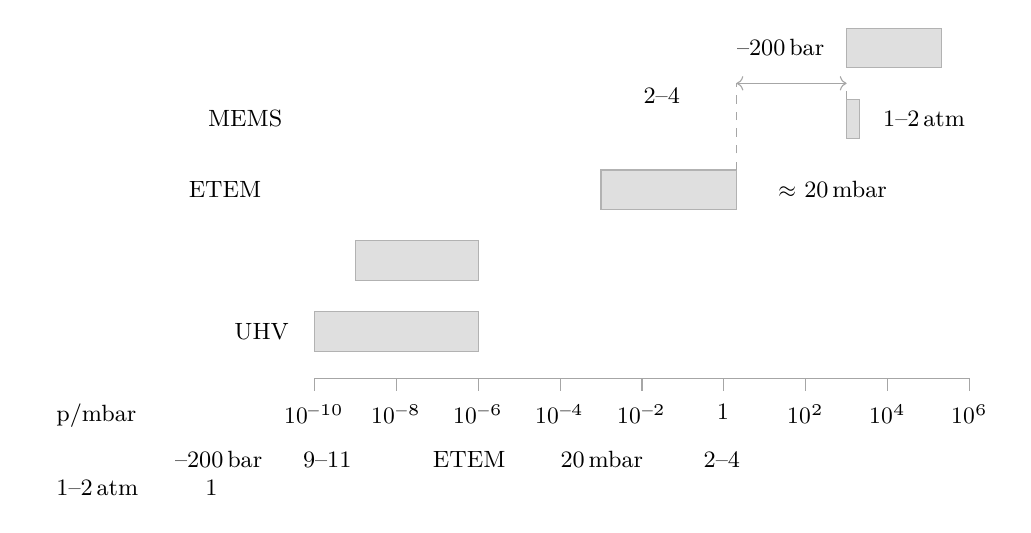
\begin{tikzpicture}[x=1mm,y=1mm,font={\fontsize{8}{9.6}\selectfont}]
% 对数压力轴：1 个数量级 = 5.2 mm，p 从 1e-10 到 1e6 mbar
\draw[gray!70] (0,-6) -- (83.2,-6);
\draw[gray!70] (0,-6) -- (0,-7.6);
\node[anchor=north] at (0,-8) {$10^{-10}$};
\draw[gray!70] (10.4,-6) -- (10.4,-7.6);
\node[anchor=north] at (10.4,-8) {$10^{-8}$};
\draw[gray!70] (20.8,-6) -- (20.8,-7.6);
\node[anchor=north] at (20.8,-8) {$10^{-6}$};
\draw[gray!70] (31.2,-6) -- (31.2,-7.6);
\node[anchor=north] at (31.2,-8) {$10^{-4}$};
\draw[gray!70] (41.6,-6) -- (41.6,-7.6);
\node[anchor=north] at (41.6,-8) {$10^{-2}$};
\draw[gray!70] (52,-6) -- (52,-7.6);
\node[anchor=north] at (52,-8) {$1$};
\draw[gray!70] (62.4,-6) -- (62.4,-7.6);
\node[anchor=north] at (62.4,-8) {$10^{2}$};
\draw[gray!70] (72.8,-6) -- (72.8,-7.6);
\node[anchor=north] at (72.8,-8) {$10^{4}$};
\draw[gray!70] (83.2,-6) -- (83.2,-7.6);
\node[anchor=north] at (83.2,-8) {$10^{6}$};
\node[anchor=north west] at (-34,-8) {p/mbar};
% 压力窗口（矩形条）
\fill[gray!25] (0,-2.5) rectangle (20.8,2.5);
\draw[gray!60] (0,-2.5) rectangle (20.8,2.5);
\fill[gray!25] (5.2,6.5) rectangle (20.8,11.5);
\draw[gray!60] (5.2,6.5) rectangle (20.8,11.5);
\fill[gray!25] (36.4,15.5) rectangle (53.6,20.5);
\draw[gray!60] (36.4,15.5) rectangle (53.6,20.5);
\fill[gray!25] (67.6,24.5) rectangle (69.2,29.5);
\draw[gray!60] (67.6,24.5) rectangle (69.2,29.5);
\fill[gray!25] (67.6,33.5) rectangle (79.6,38.5);
\draw[gray!60] (67.6,33.5) rectangle (79.6,38.5);
% 行标签
\node[anchor=east,align=right,text width=32mm] at (-2,0) {模型催化／表面科学 UHV};
\node[anchor=east,align=right,text width=32mm] at (-2,9) {电镜镜筒、电子枪};
\node[anchor=east,align=right,text width=32mm] at (-2,18) {ETEM 样品区};
\node[anchor=east,align=right,text width=32mm] at (-2,27) {封闭气体池（MEMS）};
\node[anchor=east,align=right,text width=32mm] at (-2,36) {工业催化反应};
% 条旁标注
\node[anchor=west,align=left,text width=24mm] at (55,18) {上限 $\approx$ 20\,mbar};
\node[anchor=west,align=left,text width=14mm] at (71,27) {1--2\,atm};
\node[anchor=east,align=right,text width=30mm] at (66,36) {常压--200\,bar};
% 压力落差指示
\draw[dashed,gray!70] (53.6,20.5) -- (53.6,31.5);
\draw[dashed,gray!70] (67.6,29.5) -- (67.6,31.5);
\draw[<->,gray!70] (53.6,31.5) -- (67.6,31.5);
\node[anchor=east,align=right,text width=26mm] at (52,30) {约 2--4 个数量级};
% 轴下说明
\node[anchor=north west,align=left,text width=112mm] at (-34,-14) {镜筒要求的高真空与工业催化反应（常压--200\,bar）之间隔着 9--11 个数量级。差分抽气把 ETEM 样品区提到约 20\,mbar，与工业条件仍差 2--4 个数量级；封闭气体池把可及压力提到 1--2\,atm，压力落差被压缩到 1 个数量级以内，代价是电子束两次穿过氮化硅薄膜。};
\end{tikzpicture}
\caption{透射电镜可及气体压力范围与真实催化反应条件的对照（对数标度，数值为源文给出的典型值而非某一机型的保证指标）。读者应看的不是单条数值，而是三个窗口之间的间距：镜筒真空到工业反应隔着 9--11 个数量级，差分抽气原位环境电镜把样品区提到约 20\,mbar 后仍差 2--4 个数量级，封闭气体池则把可及压力提到 1--2\,atm。压力只是「环境落差」的一个维度，温度与气体组分见 \tabref{tab:ch02c-pt}。\figsrc{据 S1 \S 2.7.5，书内 p.155--157 / PDF p.174--176 重绘}\schemamark}
\label{fig:ch02c-pressure}
\end{figure}

除差分抽气系统外，原位环境电镜还有两项配套设计，它们各自也带来新的限制。

其一是污染控制。考虑到催化反应在样品室内壁引发的分子凝聚、积炭等电镜污染问题，往往会在样品室附近配备导流式远程等离子体清洗装置，借助电镜真空系统抽气气流，将产生的等离子体注入样品室，借助氧化电离作用清除内壁上的污染物，以确保电镜的真空度和显微性能。注意这里已经埋下一条重要边界：反应体系中同时存在等离子体，而等离子体本身也会与样品作用。

其二是气体组分监测。除了在高空间分辨条件下观察催化剂结构变化，监测反应过程的气体组分变化同样是全方位获取催化反应信息不可或缺的一环。环境电镜在样品室附近设计了残余气体分析系统（residual gas analysis，RGA）：在样品附近的抽气管道，借助分子泵将少量催化剂附近的气体采样并送至质谱仪检测，给出反应中的底物和产物种类、含量等信息。值得注意的是，RGA 分析是把气体采样至镜筒外的质谱仪，由于气体跨距离传输会带来信号分析的时延，反应气体分析和催化剂显微表征难以做到完全同步。

与 RGA 对应的一种气体检测方案是借助能量损失谱：利用样品室内气体分子对电子束的能量吸收对应于气体分子轨道跃迁的特性，在 EELS 谱低能区（low loss）可以观察到对应气体分子电子能量吸收现象，这些吸收峰往往成组出现，且随气体分子不同而具有特定强度分布，故称为气体分子的「指纹峰」。通过辨识 EELS 谱中指纹峰的种类及强度，可以实现气体组分的辨识乃至定量。由于该信号是从电子束与样品附近气体直接作用产生的（原位、实时产生和记录），这一方案可以实现催化剂表面反应过程的实时、原位监测。然而它不利的一点同样明确：电镜光路工作在能量损失谱模式而非成像模式，导致分析气体组分时无法实现催化剂显微结构的成像观察。于是，「同一时刻只能看结构或只能看气氛」成为原位环境电镜的第一条硬边界。

在电镜中实现催化剂原位气相反应观察的另一个途径是借助原位气体池技术（gas cell）。该技术基于常规透射电镜，不要求在电镜中直接引入气体环境，而是借助特殊的样品杆前端设计：用 MEMS 技术特制的芯片实现精确控温，两片对电子束透明的氮化硅（Si$_3$N$_4$）薄膜将催化剂粉体封闭在微腔内，微腔设有进气、出气孔道，通过样品台与电镜外控制装置连通，通入特定气体并将其约束在反应微腔内，从而不破坏电镜样品室的真空工作环境，实现在常规电镜下的气氛反应，并透过氮化硅薄膜观察催化剂颗粒的微结构演化。

气体池解除的正是 ETEM 的压力上限：由于它需要构筑上下密封的 Si$_3$N$_4$ 薄膜微腔，薄膜强度决定了通入气体的压力，最大典型压力值可达 1--2 个大气压，优于原位环境电镜的 20\,mbar。但它引入的新限制有三条：一是为保持氮化硅薄膜的必要机械强度而增加厚度，反过来会干扰电子束的成像质量，使电镜分辨率下降；二是与 ETEM 相比，气体池中样品两侧的氮化硅薄膜会干扰 X 射线能谱和电子能量损失谱，影响催化剂的成分及电子态分析；三是基于 MEMS 技术的微腔气密性如果失控，可能带来气体泄漏，为电镜的安全运转带来隐患。

\begin{table}[htbp]
\centering
\setlength{\tabcolsep}{4pt}
\small
\caption{原位气氛反应的压力与温度边界：两种原位方案与工业反应条件的对照。读者应重点比较「压力落差」与「分析通道」两行——压力落差最小的方案（气体池）付出了薄膜干扰谱学分析的代价，而谱学通道最完整的方案（ETEM）压力上限最低。表中数值为源文给出的典型值，小分子气体的压力上限见正文的存疑标注。\src{据 S1 \S 2.7.5，书内 p.155—160 / PDF p.174—179 归纳。}}
\label{tab:ch02c-pt}
\begin{tabular}{@{}p{22mm}p{32mm}p{30mm}p{28mm}p{30mm}@{}}
\toprule
条件项 & 原位环境电镜（ETEM） & 封闭气体池（MEMS） & 工业催化反应 & 对结论的影响 \\
\midrule
反应区压力 & 典型上限约 20\,mbar；小分子气体为 10\,mbar 量级（见正文存疑标注） & 最大典型值 1--2 个大气压 & 常压--200\,bar（$10^{3}$--$10^{5}$\,mbar） & 压力改变表面覆盖度与物相稳定性，低压下的「活性相」未必是工业条件下的活性相 \\
\addlinespace
与工业压力落差 & 2--4 个数量级 & 1 个数量级以内 & --- & 落差越大，原位结论向工业条件外推的风险越高 \\
\addlinespace
观察与分析通道 & 无窗，可直接做 EDS/EELS，但与成像模式互斥 & 电子束两次穿过 Si$_3$N$_4$ 薄膜，干扰 X 射线能谱与 EELS & 不在电镜内 & 气体池测得的成分与价态需扣除薄膜影响后才可与无窗结果比较 \\
\addlinespace
加热与测温 & MEMS 芯片加热；早期芯片温度不均匀性可达近 80\,\degC & 同 MEMS 芯片控温 & 反应器整体控温，测温点在床层或壁面 & 测温误差直接进入构效关系，是原位结论最脆弱的一环 \\
\addlinespace
产物／组分监测 & RGA（跨距离传输有滞后）或 EELS 低能指纹峰 & 无在线产物分析 & 在线色谱／质谱，与反应器同步 & 电镜内的组分信息与结构信息往往不同步 \\
\bottomrule
\end{tabular}
\end{table}

在催化研究的实例方面，目前原位环境透射电镜已被广泛用于监测工作状态下的工业催化剂，其化学气氛包括还原（氢气、烃类、一氧化碳等）、氧化（氧气、二氧化碳等）或水蒸气。源文认为其中对钒磷复合氧化物催化剂的研究尤为成功：所选目标反应是正丁烷选择氧化制马来酐，氧钒基焦磷酸盐相（(VO)$_2$P$_2$O$_7$，简称 VPO）的 (201) 晶面被认为具有最高的催化活性，该活性相主要通过焙烧前驱体 VO(HPO$_4$)$\cdot$0.5H$_2$O（VHPO）制得，因此对该前驱体向活性相转化过程进行原位研究具有重要意义。在原位环境透射电镜中，将 VHPO 前驱体在氮气氛围下加热后发现，前驱体结构转变从 400\,\degC 左右开始，绝大部分的 VPO 在 450\,\degC 下生成；结合动态电子衍射分析发现，在整个结构变化过程中，所有晶体的结晶程度较高，原子排列的周期性良好，未观测到其他过渡晶相或非晶相的生成。在正丁烷气氛和典型的反应温度（约 390\,\degC）下，只有 VPO 的 (201) 晶面上的阳离子对烷烃选择氧化起作用，其微结构介于氧钒八面体和磷酸四面体之间。使用原位环境透射电镜进行催化研究的实例还包括铜催化水蒸气重整反应和纳米碳管生长。

原子分辨尺度的原位观察则更能说明「结构确在变化」。源文记载，可以观察到反应前 CeO$_2$ 负载的 Au 单晶纳米颗粒保持标准的 (100) 面间距 0.20\,nm，同时面内原子距离为 0.29\,nm；而在催化 CO 氧化过程中，表面 CO 分子吸附导致 Au 的 (100) 晶面原子发生重构，面内原子间距被压缩为 0.25\,nm，面间距离则拉伸至 0.25\,nm。此处已对照原页面图像（书内 p.158 / PDF p.177）：原书原文为「可以观察到反应前 Au 单晶纳米颗粒保持了标准的（100）面间距 0.20 nm，同时面内原子距离为 0.29 nm；而在催化 CO 氧化过程中，表面 CO 分子吸附导致 Au 的（100）晶面原子发生重构，面内原子间距被压缩为 0.25 nm，面间距离则拉伸至 0.25 nm」。重构前后两处 0.25\,nm 确为原书原文——图 2-56 中亦分别标注 0.29\,nm／0.20\,nm（真空）与 0.25\,nm／0.25\,nm（CO／空气），并非 OCR 失真；面内值原书记作 0.29\,nm（此前正文误作 0.291\,nm，已改正），「特征间距」原书作「（100）面间距」，「层间距离」原书作「面间距离」。由此可见，ETEM 手段为在原子尺度探测催化剂表面重构行为提供了有力保障。源文进一步指出，在当前技术条件下，如匹配超快电子感光相机（基于 CMOS 的电子感光元件），有望在毫秒乃至微秒尺度捕捉催化剂在反应中的原子级结构变化。另一个例子是追踪 Fe 单个颗粒在费托反应中表面 Fe$_5$C$_2$ 相的演化过程：在环境电镜中引入 CO 与 H$_2$ 的反应气氛，借助单颗粒电子衍射及暗场像技术，在反应 60\,min 内追踪了 Fe 颗粒的表面碳化、Fe$_5$C$_2$ 成型及生长过程。此处已对照原页面图像（书内 p.159 / PDF p.178）：原书原文为「在环境电镜中引入 CO 与 H$_2$ 的反应气氛，借助单颗粒电子衍射及暗场像技术［图 2-57（b）］，在反应 60 min 内追踪了 Fe 颗粒的表面碳化、Fe$_5$C$_2$ 成型及生长过程［图 2-57（a1）～（a3）］」。时间单位为 \textbf{min}（图 2-57（b）中标出的时刻为 8、9、12、40、42、60 min），此前正文因 OCR 只剩「在反应 60～ 内」而写作「60\,s 量级」，与原书不符，已改正并补出「表面碳化、Fe$_5$C$_2$ 成型及生长」三阶段与「单颗粒电子衍射及暗场像技术」。

\begin{obs}
在 CeO$_2$ 负载 Au 颗粒的 CO 氧化原位实验中，可从图像序列直接读出：（1）反应前颗粒呈单晶形貌，面内原子距离为 0.29\,nm（原书图 2-56 标值）；（2）通入 CO／空气并升温后，同一颗粒表面的原子列间距变小（面内压缩），并且沿另一方向的间距发生变化；（3）变化发生在外表面，颗粒内部仍保持原有排列。
\end{obs}

\begin{infer}
上述变化被解释为表面吸附导致 Au 的 (100) 晶面发生原子重构。这条推断依赖两个前提：一是图中所测间距的变化确实来自原子列位置而不是衬度条件的改变（欠焦、厚度、通道效应都会改变表观间距）；二是重构被归因于反应气氛，而不是电子束本身。后一个前提尤其需要对照实验来保证——见下面的误判与回查。
\end{infer}

\begin{dataflow}
原位实验的完整数据链是：设定气氛（气体种类、分压、流速）与温度（设定值 $+$ 实测值 $+$ 不确定度）$\to$ 同步采集图像／衍射／谱（并记录时间戳）$\to$ 结构变化的判读（相变温度、暴露晶面、重构前后间距）$\to$ 与同批样品的产物分析（RGA、EELS 指纹峰或离线色谱）对齐时间轴 $\to$ 建立构效关系假设 $\to$ 用宏观反应器数据检验。链条中最容易被省略、也最致命的一步是「时间轴对齐」：RGA 的传输时延与 EELS 的模式互斥，都会让「结构变化」与「产物变化」看起来同时发生，而实际并不同时。
\end{dataflow}

\begin{pitfall}
源文专列了一段「原位环境电镜表征中的注意事项」，其中每一条都可以理解为这项技术的固有代价：

（1）辐照损伤在高温高压条件下更严重。高温高压反应条件下催化剂晶体结构的电子辐照损伤较为严重；球差校正与三维重构中得到的高分辨图像同样伴随高剂量。判断「这是反应造成的结构变化还是电子束造成的」，必须做束流对照（同一条件、不同剂量率、或束流关断—开启循环）。

（2）电子束会改变气氛。气体分子可能在高速电子束作用下离子化，产生的等离子体与样品发生作用，大大影响了对催化反应的研究。这意味着电镜内的「反应条件」并不是中性的观察窗口，电子束本身是反应体系的一部分。这一条与前述等离子体清洗装置叠加在一起，使样品室内始终存在非热平衡的活性物种。

（3）温度测量的准确性与均匀性。原位环境催化反应需要在特定温度下进行，因此催化剂颗粒需要首先负载到带有 MEMS 控温芯片的氮化硅薄膜上；芯片温度测量的准确与否，直接关系到原位反应中催化剂构效关系的建立，以及与真实反应条件的参考和关联。

源文给出了一种巧妙的原位测温思路：金属受热后原子间距与电荷密度改变，进而引发体相等离子体振动频率移动；反之，借助 EELS 表征等离子体振动频移，就可以反推出 MEMS 加热微电路中的温度。同时源文提醒，对于早期生产的用于 ETEM 的控温芯片，温度均匀性令人担忧，温度差异可达近 80\,\degC，这将导致实际参数的严重偏离，误导对催化剂构效关系的认知；值得庆幸的是，随着 MEMS 技术及工艺的不断进步，控温精度及均匀度在不断提高。80\,\degC 这个数字应当被记住：在 Arrhenius 意义上，它足以把速率与选择性的比较彻底打乱，而它出现在「测温」这一环节，正好说明原位实验的误差不总是来自电镜的分辨率。
\end{pitfall}

\begin{crosscheck}
原位结论必须用三条外部证据回查：一是气氛信息的两条独立通道互查——RGA（镜筒外质谱，有传输时延）与 EELS 低能指纹峰（原位实时，但与成像模式互斥），两者给出的组分变化在时间轴对齐后应当自洽；二是两种原位方案的互查——开腔 ETEM（压力低、无窗、谱学好）与封闭气体池（压力高、有窗、谱学受薄膜干扰）在重叠压力区间内应给出相同的结构演化趋势，若不同则优先怀疑薄膜效应或压力效应；三是与宏观反应器的互查——把电镜条件下的温度、分压换算成与固定床可比的量，检查产物分布与动力学是否一致。三条互查都通过时，原位观察才构成机理证据；否则它只是「在电子束下、在某一气氛中发生过的结构变化」。
\end{crosscheck}

\paragraph{本节小结} 表~\ref{tab:ch02c-newold} 与表~\ref{tab:ch02c-situ} 把本节六项技术的「解除的旧限制／引入的新限制／适用样品」并列在一起。使用时请从右往左读：先确认样品是否落在「适用样品」一列，再确认自己是否具备「前提条件」，最后才看「解除的旧限制」这一列的宣传性表述。

\begin{table}[htbp]
\centering
\setlength{\tabcolsep}{4pt}
\small
\caption{成像与能量分辨类新技术的新旧限制对照。读者应看「引入的新限制」一列：每一项能力的代价都写在那里，而它往往就是实际实验中最先遇到问题的地方。\src{据 S1 \S 2.7.1—\S 2.7.2，书内 p.147—151 / PDF p.166—170 归纳。}}
\label{tab:ch02c-newold}
\begin{tabular}{@{}p{26mm}p{36mm}p{44mm}p{34mm}@{}}
\toprule
技术 & 解除的旧限制 & 引入的新限制 & 适用样品与前提 \\
\midrule
成像球差校正器 & 物镜球差造成的漫散圆斑与菲涅耳条纹；不必再用焦系列计算重建换取清晰度 & 只校正三阶球差，色差与更高阶几何像差成为新的分辨率瓶颈；校正器本身需要稳定的供电与环境；校正后的像仍经中间镜继续放大 & 薄样品、需晶格分辨的纳米晶与界面；束敏样品必须改用低剂量方案 \\
\addlinespace
束斑球差校正器（probe corrector） & STEM 探针无法同时做到最小束斑与足够强度，限制 HAADF 的 $Z$ 衬度分辨率（源文：0.24\,nm 提高到 0.13\,nm） & 需要计算机自动调校多级四极—八极系统；探针电流集中于极小体积，单位面积剂量升高；轻元素柱的衬度仍受 $Z$ 衬度趋势限制 & 原子分辨 HAADF-STEM、原子级 EELS/EDS、低加速电压下的束敏样品 \\
\addlinespace
Wien 单色器与高分辨能量过滤器 & 热场发射系统 0.8--1\,eV 的能量分辨率使 ELNES 精细结构湮没在谱中 & 单色器滤除大量电子（分辨率优于 0.1\,eV 时约 75\% 的场发射电子被滤掉），束流与信噪比下降；低能区定量受相对论效应与切伦科夫辐射干扰 & 过渡金属 $L_{2,3}$ 边、氧 $K$ 边等近阈精细结构；纳米半导体带隙（需修正切伦科夫项） \\
\bottomrule
\end{tabular}
\end{table}

\begin{table}[htbp]
\centering
\setlength{\tabcolsep}{4pt}
\small
\caption{三维与原位类新技术的新旧限制对照。两类技术的共同点是：解除的限制写在中间一列，而新限制往往由「样品台／样品杆」这一类硬件引入，不在电镜主体的指标表上。\src{据 S1 \S 2.7.3—\S 2.7.5，书内 p.151—160 / PDF p.170—179 归纳。}}
\label{tab:ch02c-situ}
\begin{tabular}{@{}p{26mm}p{36mm}p{44mm}p{34mm}@{}}
\toprule
技术 & 解除的旧限制 & 引入的新限制 & 适用样品与前提 \\
\midrule
三维电子断层重构 & 二维投影把三维结构特征相互覆盖，无法判断金属粒子在载体表面还是孔道内部 & 需 $\pm 80^\circ$ 大角度倾转，物镜极靴空间加大导致物镜分辨率下降（常靠球差校正器补偿）；缺失楔形使沿光轴方向失真；需上百张投影，累积剂量与漂移；原子分辨与元素／价态分辨目前不能兼得 & 多孔载体上金属粒子的空间分布与孔内／孔外比例、核壳结构的价态分区、等离基元模式分布；前提是每张投影的强度随质厚单调 \\
\addlinespace
电子全息术（双棱镜） & 一般高分辨像中相位与振幅非线性混合、衬度受相位传递函数修饰；可绕开物镜球差直接取相位 & 需高亮度、高相干性场发射源；需参考全息图与傅里叶重建；只有薄样品与弱相位近似下相位才与投影电势线性相关；相位需解缠，视场受相干宽度限制 & 纳米粒子的投影电势与内部空洞、带电粒子周围静电场、磁畴；催化体系应用仍有限（如 Au/TiO$_2$ 界面电荷传递） \\
\addlinespace
原位环境电镜（差分抽气） & 电镜高真空与催化反应气氛不相容，无法在反应中实时观察 & 样品区压力上限（典型 20\,mbar；小分子气体 10\,mbar 量级）与工业条件仍差 2--4 个数量级；气体散射电子使分辨率下降；气体电离产生等离子体参与反应；RGA 与成像不同步；EELS 指纹峰与成像模式互斥；高温高压下辐照损伤加重 & 还原／氧化／水蒸气气氛下的结构演化：VPO 前驱体相变、Au/CeO$_2$ 表面重构、Fe 费托碳化物生长 \\
\addlinespace
原位气体池（MEMS 封闭腔） & ETEM 的压力上限；可在常规电镜上实现 1--2 个大气压的气氛反应 & 为保持机械强度而加厚的 Si$_3$N$_4$ 薄膜干扰成像，分辨率下降；薄膜干扰 X 射线能谱与 EELS，影响成分及电子态分析；微腔气密性失控会漏气，威胁电镜安全 & 较高压力下的颗粒形貌与物相演化；不适用于需要无窗 EDS/EELS 定量的场合 \\
\bottomrule
\end{tabular}
\end{table}

\subsection{透射电子显微镜的局限性及注意事项}

同任何其他表征仪器一样，透射电子显微镜也有其局限性。源文把局限列为六条（投影、统计代表性、大小粒子、衬度与结构的关系、放大倍数与晶格参数、定量成分分析的精度）；本节保留这六条，并补上原位与束损伤相关的三条。为便于使用，下面把全部局限归并为五类「落差」，每一条落差都给出它在实验中的表现与缓解方式：投影效应（维数落差）、统计代表性（空间落差）、束损伤（剂量落差）、真空与真实反应条件的落差（环境落差）、样品制备改变样品本身（同一性落差）。最后给出结论前必须报告的项。

\begin{methodsum}
本节的用法不是「记住电镜不可靠」，而是「在写结论时逐条自查」。一个可操作的判据是：任何一条由电镜得出的结论，如果它能被归入下列五类落差之一而作者没有给出应对，就应当被降级为「观察到的现象」，而不是「测得的性质」。表~\ref{tab:ch02c-gaps} 给出了这五类落差的对照与报告要求。
\end{methodsum}

\subsubsection{投影效应：一张像不能回答三维问题}

电子显微像是入射电子透过试样后成的二维投影像，因此用一张电镜照片不能简单地解释试样的三维结构。尤其是催化剂比表面积大、多孔样品多，从一张投影照片不能判断出金属粒子是负载在载体表面还是在载体孔道内部。源文举的例子很典型：用纳米碳管作载体制备金属催化剂，透射电镜只能验证制备是否成功，金属粒子是否负载在纳米碳管上；虽然照片可以给出金属粒子大小、分布、形貌的信息，但并不能准确定位金属粒子是在纳米管内部或外部。在普通透射电子显微镜中，确定金属粒子是否分布在碳管内外的唯一办法就是转动样品（如 $\pm 30^\circ$）观察金属粒子相对于碳管壁的位置变化。

需要强调的是，这里的困难不是分辨率不够，而是信息维度不够：投影把沿束方向不同深度的结构叠加到一个像素上，任何「深度」方向的问题（孔内还是孔外、核壳还是混合物、表面还是体相）都不能由单张投影像回答。解决它的技术是电子断层重构，而重构又带来新限制（见 \S 2.7.3）。

\subsubsection{统计代表性：局域信息对上亿粒子}

催化反应中使用的催化剂是大量的。如果是负载型金属粒子催化剂，参加反应的金属粒子上亿。电子显微镜具有高空间分辨率，但给出的是局域信息：一张高分辨电子显微像通常只包括一两个，最多四五个金属粒子的结构像；即使低放大倍数的显微像照出的粒子数目也经常少于一百个（这与粒子的大小有关：粒子太小时，放大倍数太低不利于观察其形貌并测量其直径）。因此做电子显微镜实验时不能照一张高分辨像就做出任何结论；所照的照片一定要有代表性、重复性，不能选择照「漂亮」的区域。确定催化剂结构或相时，不要忽略利用电子衍射技术：电子衍射花样的强度通常来自于几十个或几百个粒子，这使确定催化剂结构更准确些，并更具代表性。

用电子显微技术确定催化剂的粒子大小分布时，还存在大粒子与小粒子的问题。因为在电子显微照片中大粒子的衬度清晰可辨，统计分布时一般不会漏掉；但是当载体厚度不均时，小于 2\,nm 的粒子衬度低、强度小，不易观察到。因此做统计分布时除了照大量的电子照片（包括至少几百个粒子到上千个粒子）外，还应注意不要忽略统计小粒子的尺寸，但同时也不能主观地忽略不统计大粒子。实验上，如果要把负载粒子的大小分布与催化剂制备和其催化性能联系起来，所做的统计分布必须基于大量粒子，并不能带有主观性。

注意这两条的联合后果：粒径分布是对数正态型的宽分布时，「不漏大粒子、不漏小粒子」在同一个放大倍数下无法同时满足，所以正确的做法是多个放大倍数分层统计，并在报告中给出各层统计的粒子数与判据。

\subsubsection{束损伤：观察本身会改变样品}

除样品的质厚衬度及扫描透射电子显微镜中的 $Z$ 衬度像的强度与试样的厚度或原子序数平方成正比外，电子显微像的衬度与样品的二维投影结构没有直接线性关系。这一条本身是「读图」的限制（见下一条），而与之并行的是「电子束对样品的改写」：源文在讨论原位环境电镜时明确指出，高温高压反应条件下催化剂晶体结构的电子辐照损伤较为严重，并且气体分子可能在高速电子束作用下离子化、产生的等离子体与样品发生作用，大大影响了对催化反应的研究。

以下三点是电子显微学的通行结论，源文未逐条展开，写在这里是为了让读者把「剂量」当成一个必须报告的量（而非可调的经验参数）：（1）入射电子能量（通常 80--300\,keV）远高于化学键能（几个 eV），能量通过弹性与非弹性散射沉积在样品中，可造成原子位移（knock-on）、溅射、局部升温、键断裂、物种迁移与非晶化；（2）氧化物、分子筛、金属有机框架、碳材料与含有机配体的体系对剂量尤其敏感，而催化剂往往正属于这些类别；（3）因此在「看得见」与「没改变」之间存在一条权衡线，只能通过低加速电压、低剂量率、直接电子探测器、以及足够的重复实验来换取，不能通过事后解释来消除。

操作上的最低要求是设置束流对照：在同一区域连续采集若干张像，比较第一张与最后一张；或在同一条件下改变剂量率重复实验。若结构变化只在第二张之后出现，它更可能是束损伤而不是本征结构。

\subsubsection{真空与真实反应条件的落差}

这是原位技术带来的落差，也是把电镜结论外推到催化反应时最容易断裂的一环。镜筒需要高真空（电子枪区在 $10^{-6}$\,mbar 以下量级），而工业催化反应在常压到 200\,bar（$10^{3}$--$10^{5}$\,mbar）进行，两者相差 9--11 个数量级。差分抽气把样品区压力提到约 20\,mbar（图~\ref{fig:ch02c-pressure}），与工业条件仍差 2--4 个数量级；封闭气体池把可及压力提到 1--2\,atm，压力接近了，但样品被两片 Si$_3$N$_4$ 薄膜封闭，电子束与 X 射线都要穿过薄膜，谱学分析的通道被削弱。

更重要的是，压力不是唯一的变量。工业反应器中还存在气体组成梯度、停留时间分布、传热与颗粒团聚状态，以及成型体的尺寸效应；这些在电镜里都不存在。电镜看到的是「单个或少量颗粒、在准静态气氛中、在电子束照射下」的行为。因此原位结果的正确用法是作为机理假设的产生器与证伪工具（例如确认某一活性相在反应气氛下是否稳定），而不是反应器行为的直接测量。凡是用原位像直接给出反应速率、选择性的做法，都需要与宏观反应器数据交叉验证。

\subsubsection{样品制备改变样品本身}

电子透明性要求把样品做成薄区（高分辨观察通常需要几十纳米甚至更薄），而催化剂在使用状态下是微米到毫米级的颗粒或成型体。把样品变成「电镜可见」的过程本身会改变它：研磨与离子减薄会引入缺陷、非晶层与表面终止的改变；超声分散与滴涂会破碎孔结构、改变颗粒的团聚状态与暴露晶面的比例；载体的孔道与金属粒子的空间关系也可能在制样中被改变——这恰好与投影效应耦合在一起，使「粒子在孔内还是孔外」的判断同时受制于制样与投影。

原位实验还有额外一层：为了用 MEMS 芯片控温，催化剂粉体必须负载到氮化硅薄膜或芯片上，其传热方式、气氛接触方式与工业成型体不同。

这一条源文没有单列，本节据 \S 2.7.5 的制样要求与 \S 2.8 中「样品不很薄时分析空间分辨率要下降」的论述归纳而来。它的操作含义是：报告必须写明制样方法（研磨、离子减薄、分散介质、支持膜）、可能的损伤形式，并尽可能做「不同制样方法给出同一关键结论」的对照；把电镜结论与 XRD、物理吸附、化学吸附、反应动力学等其他表征交叉验证，正是为了对冲这一落差。

\subsubsection{衬度与结构之间没有简单的线性关系}

除质厚衬度及 HAADF 的 $Z$ 衬度像的强度与试样厚度或原子序数平方成正比外，电子显微像的衬度与样品的二维投影结构没有直接线性关系。衍射衬度常带有动力学效应（即衍射束的强度会受样品厚度及试样偏离布拉格条件的大小影响），相位衬度受透镜畸变与欠焦量控制。因此高分辨像中的暗（或明）条纹不是试样的某一晶面的原子排列，而只是具有这一晶面间距的条纹像。除非在 Scherzer 欠焦时衬度传递函数在很大的空间频率范围内不改变符号，否则不能把高分辨像的亮点（或暗点）用原子排列位置解释。

这条限制直接决定了读图语言：看到周期性的条纹，可以推断「存在具有该间距的晶面族」，但不能直接推断「亮点的位置就是原子柱的位置」。把条纹像当原子像来标注原子坐标，是本卷最需要避免的过度解释之一。

\subsubsection{放大倍数、晶格参数与定量分析的精度}

电子显微镜的放大倍数（和做电子衍射时的相机长度）只是电子显微镜出厂时厂家给出的参考值。如要用电子显微镜精确测量晶格参数，一定要用标样标定放大倍数。注意在高放大倍数时，透镜激磁电流的任何微小变化都会导致电子显微镜的放大倍数（或测定的晶格间距）变化，因此照高分辨像的实验条件（如室温或冷却水的温度）都应与标定时的实验条件一致。最好的办法是用样品中已知的结构定标来测定晶格常数。另外，小粒子在倒易空间中的格子点变大（尺寸效应），所以在电子显微镜中即使小粒子不完全处于布拉格条件时也能看见其点阵条纹（对面心立方金属最常见的是 $\{111\}$ 晶面的干涉条纹）。但当粒子小于 2\,nm 时，测得的点阵间距要比金属晶体的点阵间距大得多——此时用条纹间距反推物相会系统性出错。

定量成分分析方面，现代的分析电子显微镜的定量成分分析技术已达到小于 1\% 的精确度，但这样的精确度一般都是在研究 X 射线能谱和电子能量损失谱探测极限的专门实验中得到的。因为样品几何条件的限制、计算电离截面时理论值的近似性、切除背底强度引入的误差，在平时表征催化剂试样的实验中通常达不到这样的高度：普通的分析电子显微镜的定量分析若有 5\% 的误差是不奇怪的，而且不能在试样上只取一个谱测定其成分，必须针对不同区域做定量分析并给出误差范围。

空间分辨率一侧同样有落差。现代高空间分辨率的分析电子显微术都能把电子束形成小至 1\,nm 的电子束斑和电子探针来做微区成分定量分析，包括扫描测定试样某一方向直线的化学分析；但是应该注意，当样品不是非常薄时，1\,nm 直径的电子束射到样品上与试样相互作用时，相互作用的体积空间往往要远大于 1\,nm 直径。即由于多重散射，电子束在样品内变宽，所收集的 X 射线光子信号等会来源于几纳米的作用范围，所以真正分析的试样区域通常要比电子束斑大得多。故样品不很薄时，分析电子显微镜的空间分辨率要下降。另外因为入射电子的能量通常在 100\,kV 以上，所以 X 射线能谱测定成分是样品的体相成分，不是其表面相成分——这一点对表面敏感的催化问题尤其重要：由 EDS 得到的「表面组成」其实是体相组成。

\subsubsection{结论前必须报告的项}

\begin{table}[htbp]
\centering
\setlength{\tabcolsep}{4pt}
\small
\caption{透射电镜结论的五类落差及其报告要求。读者应把右列当作投稿或内部报告前的检查清单：任何一项缺失，都要在正文中用「在本实验条件下」之类的限定语把结论收窄。\src{据 S1 \S 2.8，书内 p.160—162 / PDF p.179—181 归纳；其中「样品同一性」一条兼采 \S 2.7.5 的制样要求。}}
\label{tab:ch02c-gaps}
\begin{tabular}{@{}p{20mm}p{28mm}p{30mm}p{30mm}p{28mm}@{}}
\toprule
落差类型 & 电镜一侧 & 真实催化一侧 & 主要后果 & 报告与缓解要求 \\
\midrule
投影（维数） & 单张二维投影像 & 三维多孔颗粒与成型体 & 无法判断粒子在孔内或孔外；核壳与混合物无法区分 & 报告倾角或倾转实验；三维结论给出倾角范围、缺失楔形与体素分辨率 \\
\addlinespace
统计代表性（空间） & 一张像 1--5 个粒子；低倍像常少于 100 个粒子 & 参与反应的金属粒子上亿 & 结论依赖所选区域；$<$2\,nm 粒子易被漏计 & 分层多放大倍数统计、给出粒子总数与判据、禁止只选「漂亮」区域；结构判定用电子衍射交叉 \\
\addlinespace
束损伤（剂量） & 高分辨与谱学都需要高剂量 & 使用状态下的催化剂不承受电子束 & 观察到的变化可能是束诱导的重构、非晶化或物种迁移 & 报告剂量与剂量率；做连续采集与变剂量率对照；束敏体系改用低电压／低剂量方案 \\
\addlinespace
真空与压力（环境） & 镜筒高真空；ETEM 约 20\,mbar；气体池 1--2\,atm & 常压--200\,bar，且有组成梯度与传热 & 低压下的活性相未必是工业条件下的活性相；原位像不能直接给速率与选择性 & 报告压力、温度（含测温方法与不确定度）、气体组成与流速；与宏观反应器数据交叉验证 \\
\addlinespace
样品同一性（制样） & 薄区、分散在支持膜或芯片上 & 微米--毫米级颗粒或成型体 & 表面终止、孔结构、团聚状态与暴露晶面比例被改变 & 报告制样方法（研磨、离子减薄、分散介质、支持膜）与可能损伤；用不同制样方法做关键结论对照；与 XRD、吸附、动力学数据互查 \\
\bottomrule
\end{tabular}
\end{table}

\begin{crosscheck}
把本节压缩成一份可执行的检查清单：结论是原子的还是条纹的（衬度是否允许这样解释）？区域是几个粒子还是上千个粒子（统计是否成立）？剂量与剂量率是多少（是否做过束流对照）？压力与温度离真实条件差多远（含测温不确定度与温度均匀性）？样品是不是原来那个样品（制样与负载是否改变它）？这五问中的每一问，都必须能在报告里找到对应的数字；找不到的，结论就应当加限定语。
\end{crosscheck}

\subsubsection{结束语}

本章介绍了透射电子显微镜的基本构造、操作模式、衬度形成原理及其附属的 X 射线能谱和电子能量损失谱的基本工作原理，并对与电子显微技术有关的最新发展做了一些介绍；用所举的应用实例，讲述了如何应用透射电子显微镜对不同催化剂进行表征，并利用其所具有的高空间分辨率和高能量分辨率研究催化材料的表面结构、缺陷化学及电子能带结构。源文指出，如果能把 TEM、HRTEM、HAADF、EDS 和 EELS 结合起来用于催化材料的研究，会得到比前面讲述的几个例子更多的信息，从而指导催化剂制备、探索催化剂反应机理。电子显微学已发展成为一门专门的学科，要真正掌握这一技术并应用到催化化学中，不仅操作上要熟练，而且还要掌握好晶体学、结构化学、固体物理学和量子力学的知识。随着场发射电子显微镜的日益普及，球差校正器、电子全息术、三维电子显微术及原位环境电镜的发展，电子显微术会成为研究催化化学必不可少的工具。

\srcnote{\S 2.7--2.8 据原书第 2 章，书内 p.147--162 / PDF p.166--181；本节新绘的压力对照图与四张对照表为便于比较而作，图内数值取自源文给出的典型值。正文中凡按学科标准形式重建之处，均已逐处对照原页面图像（书内 p.147--162 / PDF p.166--181）核验，核验结论就地以「此处已对照原页面图像（书内 p.X / PDF p.Y）」的说明记于该处；未加此类说明之处，不代表已核对页面图像。}
}{}
\IfFileExists{chapters/parts/ch02-d.tex}{\input{chapters/parts/ch02-d}}{}
\IfFileExists{chapters/parts/ch02-e.tex}{\input{chapters/parts/ch02-e}}{}
}{}
\IfFileExists{chapters/ch03.tex}{% chapters/ch03.tex —— 第 3 章 热分析方法
% 装配层：只负责按顺序引入各分片。分片缺失时跳过，便于增量成书。
% 分片文件：chapters/parts/ch03-{a..e}.tex

\IfFileExists{chapters/parts/ch03-a.tex}{% ================================================================
%  chapters/parts/ch03-a.tex
%  第 3 章  热分析方法（分片 a）
%  源：S1（上册）第 3 章，书内 p.169—180 / PDF p.188—199
%  覆盖：§3.1 热分析的分类、§3.2 几种常用的热分析技术（TG / DTA / DSC / MTDSC）、
%        §3.3 热分析动力学简介（基本关系与等转化率法的前提）
%  未覆盖（由后续分片续写）：§3.4 应用、§3.5 联用技术、§3.6 实验技巧、§3.7 结束语
% ================================================================

\chapterstart{热分析方法}%
{本章回答：热分析曲线上的台阶与峰究竟对应哪些物理量，热重法（TG）、差热分析（DTA）与
差示扫描量热法（DSC）的信号含义与纵轴正负约定为何不同，什么条件下才能把一条曲线换算成
组成与热量，以及热分析求出的活化能在什么前提下才可信。§3.1 给出分类与三种主力技术的分工，
§3.2 逐个技术讲原理与读图，§3.3—§3.6 沿「测量与条件—数据到结论—误判与边界—互补与回查」
这条主线展开，§3.7 讲联用热分析（源书 §3.4—§3.7 的应用、联用、实验技巧与结束语四节已按这条主线重编）。}
\label{ch:03}

\subsection{这个方法测量什么}

\begin{probout}
热分析（thermal analysis，TA）的定义里有两个限定条件必须与「测量」二字一起读：
\textbf{程序控温}与\textbf{一定气氛}。它测量的是物质的某一物理性质随温度或时间的变化，
输出只有一条曲线，曲线本身不给出组成、结构或机理，只回答「在什么温度发生了什么变化」
\src{S1 §3.1，书内 p.171 / PDF p.190}。

按所测的物理性质，ICTA 把热分析分为九类十七种：质量（热重法）、温度（差热分析）、热量
（差示扫描量热法、温度调制式差示扫描量热法）、尺寸与力学量（热机械分析、动态热机械分析）、
声学量、光学量、电学量、磁学量，另有把两种以上技术接在一起的联用技术——TG-DTA、TG-DSC 属
同时联用，TG/MS、TG/FTIR 属串接联用，TG/GC 属间歇联用
\src{S1 §3.1 表 3-1，书内 p.171--172 / PDF p.190--191}。催化剂研究中真正用得多的只有三种，
它们的区别在\textbf{测的物理量本身}：TG 测质量、DTA 测温差、DSC 测热流（能量差）。
\end{probout}

「TG 测质量、DTA 测温差、DSC 测热流」是本章最需要记住的一句话：三者的曲线形状可以很相似，
信息含量却相差很大，而混淆往往从纵坐标开始。表~\ref{tab:ch03-three} 按五个问题把三者拆开：
测什么、纵轴方向怎么定、能给出什么、不能给出什么、定量能力到哪一步。

\begin{table}[tbp]
\centering
\caption{热重法、差热分析与差示扫描量热法的对照。读者应看两行：第二行的纵轴方向约定
（DTA 与 DSC 相反，是读图时最容易弄反的地方），以及最后两行的能力边界——差异的根源在于
DTA 的信号是温差、DSC 的信号是热流，二者之间隔着一个需要标定的热阻。\src{据 S1（上册）
§3.2.2—§3.2.3，书内 p.171--177 / PDF p.190--196 归纳；原书表 3-1 为「热分析技术分类」
（ICTA 将热分析技术分为 9 类 17 种），与本表无对应关系，故此处只引正文。}}
\label{tab:ch03-three}
{\srcsize
\begin{tabularx}{\textwidth}{@{}lXXX@{}}
\toprule
项目 & 热重法 TG & 差热分析 DTA & 差示扫描量热法 DSC \\
\midrule
直接测量的物理量 & 试样质量 $m$，信号为变化量 $\Delta m$ & 试样与参比物的温度差 $\Delta T$ & 输给试样与参比物的能量差，即热流率 $\mathrm{d}Q/\mathrm{d}t$ \\
纵轴方向约定 & 向上为质量增加、向下为质量减小；DTG 失重峰朝下 & 习惯约定：向上放热、向下吸热 & 热力学惯例：向上为正＝吸热、向下为负＝放热 \\
能给出什么 & 台阶的温度区间与失重百分数、残余量、起始分解温度（表征热稳定性）；由台阶高度反推组成 & 热事件的温度与先后次序、吸热或放热的性质；ICTA 规定用外推起始温度表示反应起始温度 & 热事件的定量热焓 $\Delta H$（峰面积）、比热容、转化率—温度（时间）关系；经标定后可溯源 \\
不能给出什么 & 无质量变化的相变（熔化、晶型转变）；逸出气体的种类；同一温区内重叠失重过程的分辨 & 热量：峰面积的比例系数含装置热阻与样品热容，未经标定不能积分成 $\Delta H$；峰温不能作鉴定物质的特征温度 & 无热效应的质量变化；逸出气体的种类；定量准确度依赖温度与热量两项标定 \\
定量能力 & 定量（质量可直接溯源到天平） & 通常只能定性或半定量 & 定量，峰面积可换算为 $\unit{J.g^{-1}}$ \\
\bottomrule
\end{tabularx}}
\end{table}

三者的差别不只是「测的量不同」，而决定了各自能支撑什么结论。TG 的纵坐标是质量，质量可以
直接溯源到天平，台阶高度就是失重百分数；DSC 的纵坐标是热流率，经温度与热量两项标定后峰
面积可以换算成热焓，也是定量技术。DTA 的纵坐标是温差 $\Delta T$，而 $\Delta T$ 与热流率
之间隔着一个热阻：同样的放热速率，在不同装置、不同样品量、不同温度下产生的 $\Delta T$
可以相差数倍。未经逐条件标定的 DTA 峰面积不能直接换算成热量——这正是 DSC 被发展出来的
原因，也是「DSC 能做定量、DTA 通常只能定性」的根本差别
\src{S1 §3.2.3，书内 p.177 / PDF p.196}。读图前必须先看纵轴标注与方向约定，否则会把分解
（吸热）与燃烧（放热）的归属整个弄反。

\subsection{核心原理与公式}

\begin{principle}
三种技术的信号都来自试样与环境的能量交换，但取信号的环节不同。TG 取的是\textbf{质量}这一
状态量，信号不经过任何热传递假设，因此最直接；DTA 取的是试样与参比物的\textbf{温差}，
DSC 取的是为维持二者温度相等而输入试样的\textbf{补偿功率}（热流率）。后两者都要经过热传递
环节：DSC 用补偿把这一环节的系数固定下来并加以标定，DTA 没有这一步，所以同一个热事件在
两种仪器上的峰高不可比、在 DTA 上甚至不可积分。
\end{principle}

\subsubsection{热重法（TG）与微商热重（DTG）}

TG 的仪器通称热天平，基本单元是微量电子天平（或石英微天平）、炉子、温度程序器、气氛控制
器与记录系统。记录方式值得注意：仪器先同时存储质量、温度与时间三组数据，测量结束后再由
时间换算成温度 \src{S1 §3.2.1，书内 p.174 / PDF p.193}。这意味着温度滞后会直接进入数据，
而不只是影响显示。

TG 曲线的读法只有两条规则：\textbf{水平段（平台）表示质量恒定，斜率发生变化的段落表示质量
变化}；纵坐标向上表示质量增加、向下表示质量减小。微商热重曲线（DTG 曲线）是质量变化率
$\mathrm{d}m/\mathrm{d}t$ 对温度或时间的图，质量减小时峰朝下。DTG 与 TG 的对应关系是严格的：
DTG 峰的起止点就是 TG 台阶的起止点，峰的数目等于台阶的数目，峰位（最大失重速率处）与 TG
曲线的拐点相对应 \src{S1 §3.1，书内 p.173 / PDF p.192；§3.2.1，书内 p.175 / PDF p.194}。
曲线上可直接读出的量有四个：台阶高度 $\Delta m$、质量变化速率 $\mathrm{d}m/\mathrm{d}t$、
质量开始变化的起始分解温度 $T_{\mathrm{i}}$（用来表征样品的热稳定性）与 DTG 峰温
$T_{\mathrm{p}}$。\textbf{这里的「四个」按原页面图像核对}（书内 p.175 / PDF p.194）：原书在同一段
逐条定义 $\Delta m$、$\mathrm{d}m/\mathrm{d}t$、$T_{\mathrm{i}}$、$T_{\mathrm{p}}$ 四项；
原书记质量用 $W$（该页前文印 $\mathrm{d}W/\mathrm{d}t$ 与 $\mathrm{d}^{2}W/\mathrm{d}t^{2}=0$），
同段的定义句又写 $m$，译文取 $m$。

用失重分数（转化率）$\alpha$ 可以把台阶高度写成与取样量无关的形式：

\begin{equation}\label{eq:ch03-alpha}
\alpha=\frac{m_0-m_t}{m_0-m_\infty}
\end{equation}

式中 $m_0$ 为初始质量，$m_t$ 为温度 $T$（或时间 $t$）时的质量，$m_\infty$ 为过程结束后的
残余质量。$\alpha=0$ 对应未反应，$\alpha=1$ 对应过程结束。

\textbf{这个式子的来源。}此处已对照原页面图像（书内 p.174--175 / PDF p.193--194）：原书 §3.1
只逐条定义 $\Delta m$（质量的变化量）、$\mathrm{d}m/\mathrm{d}t$（质量变化的速率）、
$T_{\mathrm{i}}$（起始分解温度）与 $T_{\mathrm{p}}$（DTG 峰温），\textbf{没有}给出以 $m_0$、
$m_t$、$m_\infty$ 表示的转化率定义式；原书直到 §3.3 的动力学方程才用到 $\alpha$，并只在变量
说明里写「$\mathrm{d}\alpha$ 为转化率」（书内 p.180 / PDF p.199）。因此本式是改编本补出的
定义（量的含义与通用约定一致），用它可以不依赖取样量地表示台阶高度。

\begin{keycond}
式~\eqref{eq:ch03-alpha} 要求 $m_\infty$ 有确定值，即曲线上存在明确的终止平台。若后续温区
仍有失重，或相邻台阶彼此重叠，$m_\infty$ 就成了人为选定的数，$\alpha$ 随之失去意义。此时
应改用绝对失重百分数 $\Delta m/m_0$，并写明用于确定基线（平台）的温区。TG 上真正能定量的
是台阶高度，能不能把它换算成组成，取决于终止平台是否真实存在，而不取决于天平的分辨率。
\end{keycond}

\subsubsection{差热分析（DTA）}

DTA 的原理是「同炉同时加热、比较两个温度」：试样与参比物处于相同的加热或冷却条件下，两支
测温热电偶分别插在试样与参比物中，输出二者随温度变化的温差 $\Delta T$。试样无变化时二者
温度相等、$\Delta T=0$；试样发生吸热或放热变化时二者温度不等，输出温差信号，经放大后记录，
这就构成了 DTA 的基本原理 \src{S1 §3.2.2，书内 p.175 / PDF p.194}。参比物必须在所测温区内
不发生热效应，这是 DTA 实验成立的前提，也是测量与条件一节要单独交代的原因。

DTA 曲线上的特征量在原书中逐条给出：\textbf{基线}（曲线上 $\Delta T$ 近似等于 $0$ 的区段，
如 $abd$）、\textbf{峰}（曲线离开基线又回到基线的部分，峰向下为吸热峰，向上则相反）、
\textbf{峰宽}（曲线偏离基线又返回基线两点间的距离或温度间距，如 $ab$）、\textbf{峰高}
（试样和参比物之间的最大温度差，即峰顶至内插基线间的垂直距离，如 $ce$）、
\textbf{峰面积}（峰和内插基线之间所包围的面积，如 $abc$）、\textbf{外推始点}
（峰的起始边陡峭部分的切线与外延基线的交点，如 $T_{\mathrm{ei}}$ 点）、
\textbf{峰温} $T_{\mathrm p}$
\src{S1 §3.2.2，书内 p.176--177 / PDF p.195--196}。其中两条结论直接决定读图习惯。

\textbf{峰温不能当特征温度用。}峰顶温度只表示试样与参比物温差最大的一点，它既不等于反应的
终止温度，位置又受试样条件影响较大，因此一般不能作为鉴定物质的特征温度，只有在试样条件
相同时才可作相对比较 \src{S1 §3.2.2，书内 p.177 / PDF p.196}。

\textbf{起始温度用外推始点。}ICTA 对大量试样的测定结果表明，外推起始温度与其它实验测得的
反应起始温度最为接近，因此规定用外延起始温度表示反应的起始温度（同一页）。这与上一条互为
补充：一个位置（峰温）不可作特征温度，另一个位置（外推始点）才是可比的起点。

\textbf{峰面积与热量之间差一个比例系数}：

\begin{equation}\label{eq:ch03-dta}
\Delta H=\frac{K}{m}\int_{t_1}^{t_2}\Delta T\,\mathrm{d}t
\end{equation}

式中 $K$ 为比例系数，与装置热阻、样品热导率、热容及温度有关；$m$ 为试样质量。$K$ 不由几何
量决定，只能逐条件标定。未标定时式~\eqref{eq:ch03-dta} 只能用于同一装置、同一条件下不同
样品之间的相对比较。

此处已对照原页面图像（书内 p.176 / PDF p.195 与书内 p.177 / PDF p.196）：原书 §3.2.2 只逐条定义
了 DTA 曲线的基线、峰、峰宽、峰高、峰面积、外推始点与峰温（上一段已按原页补齐），
\textbf{并未给出峰面积与热量之间的换算关系}，原书全节没有出现符号 $K$、$m$，也没有积分式；
式~\eqref{eq:ch03-dta} 是本改编本补出的通用定量关系（峰面积正比于热效应，比例系数只能逐条件
标定），不是原书内容。原书此处的配图为图~3-3（热电偶和温差热电偶）与图~3-4（典型 DTA
曲线）。另：原书该段自身在「外推起始温度」与「外延起始温度」两种写法间混用，译文照录。

\subsubsection{差示扫描量热法（DSC）}

DSC 是为克服 DTA 在定量测定上的不足而发展起来的。它测量与试样热容成比例的单位时间功率输出
与程序温度或时间的关系，做法上完成了 DTA 做不到的一件事：\textbf{及时补偿试样因热效应产生
的能量变化，使试样与参比物之间的温度始终保持相同}——无温差、无热传递，热损失小、检测信号
大，因此灵敏度与精度都大幅提高，可以进行热量的定量分析
\src{S1 §3.2.3，书内 p.177 / PDF p.196}。

DSC 量热仪分两类。\textbf{功率补偿型}采用零点平衡原理，又分外加热与内加热两种：外加热式把
试样和参比物放在外加热炉内加热，二者容器下各装一组独立的补偿加热丝与传感器，两个控制系统
分别负责按预定速率升降温、以及补偿二者之间产生的温差（试样出现温差时改变补偿加热丝的电流）；
内加热式不设外加热炉，直接用两个小加热器加热并同时进行功率补偿。\textbf{热流型}仍按差热
分析的原理做量热，分热流式与热通量式；热通量式的检测器由许多热电偶串联成热电堆式热流量计，
两个热流量计反向连接，分别安装在试样容器、参比容器与炉体加热块之间，热端均匀分布在容器壁
上，因此检测信号大、测得的试样温度是试样各点温度的平均值，重复性、灵敏度与精确度都高，
常用于精密的热量测定 \src{S1 §3.2.3，书内 p.177--178 / PDF p.196--197}。

DSC 曲线的纵坐标是热流率 $\mathrm{d}Q/\mathrm{d}t$，单位 $\unit{mW}$（即
$\unit{mJ.s^{-1}}$），横坐标是温度或时间；按热力学惯例，向上为正、表示吸热效应，向下为负、
表示放热效应 \src{S1 §3.1，书内 p.173 / PDF p.192}。峰面积给出热焓：

\begin{equation}\label{eq:ch03-dsc}
\Delta H=\frac{1}{m}\int_{t_1}^{t_2}
\left[\frac{\mathrm{d}Q}{\mathrm{d}t}
-\left(\frac{\mathrm{d}Q}{\mathrm{d}t}\right)_{\mathrm{base}}\right]\mathrm{d}t
\end{equation}

积分区间从峰的外推始点到外推终点，括号内是被测信号与基线之差。与式~\eqref{eq:ch03-dta}
相比，关键差别在于热流率与功率之间的关系由仪器标定给出，不必像 DTA 那样每次实验重新确定
一个与装置和样品都相关的 $K$，所以峰面积可以直接换算成 $\unit{J.g^{-1}}$。

\textbf{原书 DSC 曲线的「数学表达式」。}此处已对照原页面图像（书内 p.178 / PDF p.197）：原书
§3.2.3 的「2. 差示扫描量热曲线」只印一句 $\mathrm{d}H/\mathrm{d}t=f(T)$ 或 $f(t)$，并说明以
热流率为纵坐标的曲线与 DTA 相似、不再重复，\textbf{没有}给出峰面积与热焓之间的换算式；原书把
热流率记作 $\mathrm{d}H/\mathrm{d}t$，本稿统一记作 $\mathrm{d}Q/\mathrm{d}t$（纵坐标
$\unit{mW}$ 的口径不变）。式~\eqref{eq:ch03-dsc} 是改编本补出的定量关系。

\begin{keycond}
式~\eqref{eq:ch03-dsc} 成立需要三个条件：一是温度与热量两项标定在测量前完成，且在测量温区
内有效；二是基线由同条件下的空白（空坩埚、同升温速率、同气氛）确定，不能凭肉眼在两段平台
之间任意连线；三是峰的外推始点与外推终点可辨识，重叠峰必须先分峰，否则应改用其它方法。
灵敏度提高不等于准确度提高：微量样品热容小、信噪比好，但称量误差与热接触差异会同步放大，
报 $\Delta H$ 时应给出重复测量的次数与分散度。
\end{keycond}

\subsubsection{温度调制式差示扫描量热法（MTDSC）}

MTDSC 在传统线性变温程序上叠加一个正弦振荡温度程序，使热流量与温度信号形成非线性调制，
从而把总热流信号分解成可逆与不可逆两种成分 \src{S1 §3.2.4，书内 p.178 / PDF p.197}：

\begin{equation}\label{eq:ch03-mtdsc}
T(t)=T_0+\beta t+A_T\sin(\omega t),\qquad
\frac{\mathrm{d}Q}{\mathrm{d}t}=C_p\frac{\mathrm{d}T}{\mathrm{d}t}+f(T,t)
\end{equation}

式中 $T_0$ 为起始温度，$\beta$ 为基础（线性）升温速率，$A_T$ 为调制幅度，$\omega$ 为调制
角频率，$C_p$ 为试样热容。第一项与升温速率成正比，经傅里叶变换后落在调制频率上，对应与
热容有关的\textbf{可逆}热流成分（玻璃化转变、大多数熔融）；第二项只与温度和时间有关，对应
动力学控制的\textbf{不可逆}成分（蒸发、挥发、结晶、热固化、分解与部分熔融）。分解效果主要
取决于三个量的选择：基础升温速率、调制周期与调制幅度
\src{S1 §3.2.4，书内 p.179 / PDF p.198}。

\textbf{原书的对应式。}此处已对照原页面图像（书内 p.179 / PDF p.198）：原书印
$\mathrm{d}H/\mathrm{d}t=C_p\,\mathrm{d}T/\mathrm{d}t+f(T,t)$，并说明第一项为可逆部分
（包括热容、玻璃化转变及大多数熔融）、$f(T,t)$ 为不可逆部分（包括焓恢复、挥发、结晶、
热固化、蛋白质变性、淀粉凝胶、分解和一些熔融）；本稿把热流率记作 $\mathrm{d}Q/\mathrm{d}t$，
故第二式与原书逐项同形而符号不同。前半的正弦温度程序
$T(t)=T_0+\beta t+A_T\sin(\omega t)$ 是改编本补出的写法——原书只用文字说明「在传统线性变温
基础上叠加一个正弦振荡温度程序」并给出图 3-8，没有印出该式。

MTDSC 的曲线形状与普通 DSC 完全一样，总热流等同于普通 DSC 的结果，额外得到的是分离后的
两条分量曲线：基础升温速率缓慢使分辨率提高，瞬时升温速率快使灵敏度提高，一次实验同时得到
比热容与热流，这是它的独特之处 \src{S1 §3.2.4，书内 p.179--180 / PDF p.198--199}。需要
注意的是，可逆与不可逆的划分是按\textbf{对升温速率的响应方式}做的操作划分，不是热力学上的
可逆性；同一变化在不同调制参数下可能落入不同分量，因此报告分量曲线必须同时给出这三个参数，
并与普通 DSC 的总热流曲线对照检查。

\subsubsection{热分析动力学的基本关系}

程序控温可分为等温与非等温两种，由于后者具有独特优点，已逐渐成为热分析动力学的核心。一般
所采用的不定温、非均相反应的动力学方程为（原书给出的是以温度为自变量的形式）
\src{S1 §3.3，书内 p.180 / PDF p.199}：

\begin{equation}\label{eq:ch03-rate}
\frac{\mathrm{d}\alpha}{\mathrm{d}t}=k(T)f(\alpha)
\qquad\Longleftrightarrow\qquad
\frac{\mathrm{d}\alpha}{\mathrm{d}T}=\frac{1}{\beta}k(T)f(\alpha)
\end{equation}

式中 $\alpha$ 为转化率（式~\eqref{eq:ch03-alpha}），$\beta=\mathrm{d}T/\mathrm{d}t$ 为升温
速率，$k(T)$ 为速率常数的温度关系式，$f(\alpha)$ 为反应机理函数。速率常数的温度关系取
Arrhenius 形式：

\begin{equation}\label{eq:ch03-arrh}
k(T)=A\exp\!\left(-\frac{E_{\mathrm{a}}}{RT}\right)
\end{equation}

$A$ 为指前因子，$E_{\mathrm{a}}$ 为活化能，$R$ 为气体常量，$T$ 为热力学温度。把
式~\eqref{eq:ch03-arrh} 代入式~\eqref{eq:ch03-rate} 并分离变量积分，得到等转化率法的出发点：

\begin{equation}\label{eq:ch03-integral}
g(\alpha)=\int_0^{\alpha}\frac{\mathrm{d}\alpha}{f(\alpha)}
=\frac{A}{\beta}\int_0^{T}\exp\!\left(-\frac{E_{\mathrm{a}}}{RT}\right)\mathrm{d}T
\end{equation}

\textbf{这两式与原书的关系。}此处已对照原页面图像（书内 p.180--181 / PDF p.199--200）：原书
§3.3 只印以温度为自变量的动力学方程
$\mathrm{d}\alpha/\mathrm{d}T=(1/\beta)k(T)f(\alpha)$（即上式右半，逐字同形），随后给出
Ozawa--Flynn--Wall（$\mathrm{d}(\lg\beta)/\mathrm{d}(1/T)=-0.4567E/R$）、Kissinger
（$\mathrm{d}[\ln(\beta/T_{\mathrm{p}}^{2})]/\mathrm{d}(1/T_{\mathrm{p}})=-E/R$）与
Freeman--Carroll 三种处理方法，\textbf{没有}印 Arrhenius 形式的 $k(T)$，也没有印积分式
$g(\alpha)$；式~\eqref{eq:ch03-arrh} 与式~\eqref{eq:ch03-integral} 是改编本按学科标准形式补出
的两步（原书以 $E$、$k(T)$ 直接进入作图法，未展开这两式）。另：原书该处的变量说明把升温速率
写成「$\mathrm{d}T$」而式中用的是 $\beta$，原书写法记于勘误乙类 B13。

\begin{keycond}
\textbf{（1）单一升温速率下求出的 $E_{\mathrm{a}}$ 不可靠。}式~\eqref{eq:ch03-rate} 中有
$A$、$E_{\mathrm{a}}$ 与机理函数 $f(\alpha)$ 三组未知量，在一条曲线上它们的作用是耦合的：
把 $E_{\mathrm{a}}$ 调大、同时换一个 $f(\alpha)$，可以在同等程度上拟合同一条曲线。因此
单条 TG 曲线给出的「活化能」既依赖所设机理函数，也依赖拟合所选温区，数值可以相差很多。
原书的做法是用 $4$ 个以上不同的升温速率测定同一系列曲线，得到一组随升温速率提高而向高温
推移的 TG 曲线，再由斜率求 $E_{\mathrm{a}}$ \src{S1 §3.3，书内 p.180--181 / PDF p.199--200}。
\textbf{（2）动力学三要素必须同时确定。}$E_{\mathrm{a}}$、$A$ 与 $f(\alpha)$ 共同决定
$\mathrm{d}\alpha/\mathrm{d}t$；只报一个活化能而不给机理函数与指前因子，别人无法复现任何
一条曲线，也无法外推到别的温度程序。\textbf{（3）等转化率法的前提是同一 $\alpha$ 处机理
不变。}若求得的 $E_{\mathrm{a}}$ 随 $\alpha$ 明显变化，说明过程中机理发生了改变，或存在
扩散控制与重叠反应，此时把它当作单一常数使用没有意义。上述三条是方法本身的性质，不是实验
误差；原书 §3.3 未逐条写明，此处按方程组的数学结构补入
\supp{原书 p.180--181 只给出动力学方程与作图法，未展开上述前提与失效判据；本条为编写组按
学科通行判定整理（2026-02），未引外部文献}。
\end{keycond}

\textbf{等转化率法的基本思想。}式~\eqref{eq:ch03-integral} 的左边 $g(\alpha)$ 只与转化率
有关，右边只与温度程序有关。在若干个升温速率 $\beta_1,\beta_2,\dots,\beta_n$ 下各测一条
曲线，取同一转化率 $\alpha$ 处的温度 $T_{\alpha,i}$，则 $g(\alpha)$ 对所有这些实验是同一个
值——于是可以\textbf{在不预设机理函数 $f(\alpha)$ 的前提下把它消去}，由 $\ln\beta_i$ 对
$1/T_{\alpha,i}$ 的线性关系直接求出 $E_{\mathrm{a}}$。Ozawa--Flynn--Wall 法是在固定的
$\alpha$ 处使用这一关系，通常由 $4$ 个以上不同升温速率的 TG 曲线作图；Kissinger 法则取每条
曲线的峰值温度 $T_{\mathrm{p}}$ 作为某个特定转化率所对应的温度，用同类的线性化关系求
$E_{\mathrm{a}}$ \src{S1 §3.3，书内 p.180--181 / PDF p.199--200}。两种方法的具体线性化公式，
以及 Freeman--Carroll 等由单条曲线同时求 $E_{\mathrm{a}}$ 与反应级数的方法，见后文 §3.3 续。

\subsection{测量与条件}

\begin{measure}
\textbf{样品。}样品量决定传热滞后：量大则试样内部温度梯度大、峰变宽、峰温向高温移动、相邻
峰合并。常规筛选用几毫克至十几毫克；动力学测量与重叠峰的分离要求更少，并尽量铺成薄层、
颗粒细小、与坩埚底良好接触。\textbf{坩埚。}常用铂、铝、石英与刚玉坩埚
\src{S1 §3.2.1，书内 p.174 / PDF p.193}；坩埚材料不得与样品或气氛发生反应（见后文误判
第（5）条）。加盖可抑制挥发、提高峰的分辨，但会改变产气过程的自生分压，凡涉及产气的定量
必须写明是否加盖。\textbf{气氛。}TG 可在静态或流动态下进行；静态条件下反应生成的气体会在
试样周围累积，试样反应速率随产物的分压而变，因此一般建议在动态气流下测量。常用气体有
\ce{Ar}、\ce{N2}、\ce{O2}、空气、\ce{CO2}、\ce{H2}、\ce{Cl2}
\src{S1 §3.2.1，书内 p.174 / PDF p.193}。气氛是实验条件的一部分：同一催化剂在空气中测到的
放热峰，在氮气中常常消失。\textbf{升温速率。}$\qtyrange{1}{20}{K.min^{-1}}$ 是常规范围，
速率越快灵敏度越高、分辨率越低、峰温越向高温移动；动力学测量至少需要 $4$ 个升温速率。
\textbf{校准。}温度用高纯金属（\ce{In}、\ce{Sn}、\ce{Zn} 等）的熔点标定，热量用已知熔化焓
的标样或蓝宝石比热标定，TG 用标准砝码标定；DSC 的基线用空坩埚在同程序、同气氛下测空白
确定。\textbf{报告。}升温速率、气氛与流量、样品量、坩埚材料与是否加盖是曲线可比性的前提，
缺任何一项，别人都无法重复这条曲线。
\end{measure}

\subsection{数据到结论}

\begin{figure}[tbp]
\centering
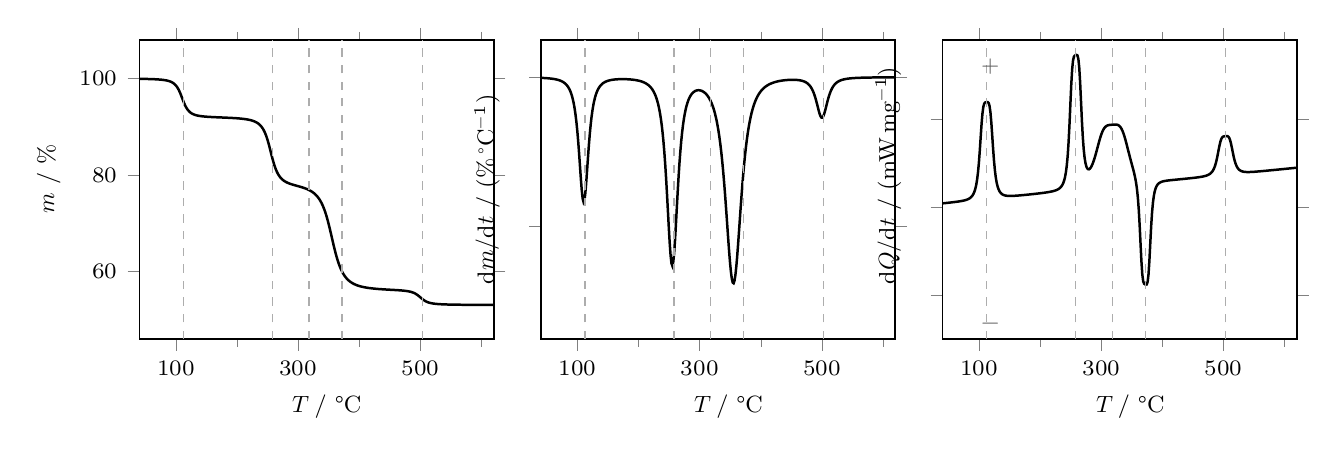
\begin{tikzpicture}
% declare function 要用 \tikzset 在 tikzpicture 层声明，图内所有 axis 才能共用。
% （放进单个 \nextgroupplot 只对该子图有效 → Unknown function；
%   放进 \begin{groupplot}[...] 又不是合法的 group 键 → I do not know the key。
%   两种写法本项目都实际踩过。）
\tikzset{declare function={
  stp(\u,\w)=0.5*(1+\u/sqrt(\u*\u+\w*\w));
  dtp(\u,\w)=0.5*\w*\w/((\u*\u+\w*\w)*sqrt(\u*\u+\w*\w));
  tgm(\x)=100-8*stp(\x-110,12)-14*stp(\x-255,14)-22*stp(\x-355,20)-3*stp(\x-500,14);
  dtm(\x)=-(8*dtp(\x-110,12)+14*dtp(\x-255,14)+22*dtp(\x-355,20)+3*dtp(\x-500,14));
  dsm(\x)=0.02+0.00035*(\x-40)
    +0.55/(1+((\x-112)*(\x-112)/121)*((\x-112)*(\x-112)/121))
    +0.75/(1+((\x-258)*(\x-258)/100)*((\x-258)*(\x-258)/100))
    +0.35/(1+((\x-318)*(\x-318)/784)*((\x-318)*(\x-318)/784))
    -0.60/(1+((\x-372)*(\x-372)/81)*((\x-372)*(\x-372)/81))
    +0.22/(1+((\x-503)*(\x-503)/169)*((\x-503)*(\x-503)/169));
}}
\begin{groupplot}[
  % 【overfull 修正】原为 width=48mm + horizontal sep=8mm：
  % 3×48 + 2×8 = 160 mm，再加 ylabels at=edge left 的左侧轴标签与刻度约 15 mm
  % 共约 175 mm，超出单栏版心 165 mm 约 10 mm ——正是实测的 29.82 pt。
  % 改为 3×45 + 2×6 = 147 mm，含左侧标签约 162 mm，留 3 mm 余量。
  group style={group size=3 by 1, yticklabels at=edge left, ylabels at=edge left,
               xlabels at=edge bottom, horizontal sep=6mm},
  width=45mm, height=38mm,
  xmin=40, xmax=620,
  xtick={100,300,500}, minor xtick={200,400,600},
  xlabel={温度 $T$ / $\degC$},
  scale only axis
]
\nextgroupplot[ymin=46, ymax=108, ytick={60,80,100},
  ylabel={质量 $m$ / \%}]
\addplot[domain=40:620,samples=400,mainline,black]{tgm(x)};
\draw[accentsoft,dashed,thinline] (axis cs:112,46) -- (axis cs:112,108);
\draw[accentsoft,dashed,thinline] (axis cs:258,46) -- (axis cs:258,108);
\draw[accentsoft,dashed,thinline] (axis cs:318,46) -- (axis cs:318,108);
\draw[accentsoft,dashed,thinline] (axis cs:372,46) -- (axis cs:372,108);
\draw[accentsoft,dashed,thinline] (axis cs:503,46) -- (axis cs:503,108);
\node[anchor=south,color=accent] at (axis cs:112,103) {①};
\node[anchor=south,color=accent] at (axis cs:258,103) {②};
\node[anchor=south,color=accent] at (axis cs:345,103) {③};
\node[anchor=south,color=accent] at (axis cs:503,103) {④};

\nextgroupplot[ymin=-0.70, ymax=0.10, ytick={0,-0.4},
  ylabel={$\mathrm{d}m/\mathrm{d}t$ / (\%\,$^{\circ}$C$^{-1}$)}]
\addplot[domain=40:620,samples=400,mainline,black]{dtm(x)};
\draw[accentsoft,dashed,thinline] (axis cs:112,-0.70) -- (axis cs:112,0.10);
\draw[accentsoft,dashed,thinline] (axis cs:258,-0.70) -- (axis cs:258,0.10);
\draw[accentsoft,dashed,thinline] (axis cs:318,-0.70) -- (axis cs:318,0.10);
\draw[accentsoft,dashed,thinline] (axis cs:372,-0.70) -- (axis cs:372,0.10);
\draw[accentsoft,dashed,thinline] (axis cs:503,-0.70) -- (axis cs:503,0.10);
\node[anchor=west,color=accent] at (axis cs:60,-0.40) {峰朝下＝失重};

\nextgroupplot[ymin=-0.75, ymax=0.95, ytick={-0.5,0,0.5},
  ylabel={热流率 $\mathrm{d}Q/\mathrm{d}t$ / (mW\,mg$^{-1}$)}]
\addplot[domain=40:620,samples=400,mainline,black]{dsm(x)};
\draw[accentsoft,dashed,thinline] (axis cs:112,-0.75) -- (axis cs:112,0.95);
\draw[accentsoft,dashed,thinline] (axis cs:258,-0.75) -- (axis cs:258,0.95);
\draw[accentsoft,dashed,thinline] (axis cs:318,-0.75) -- (axis cs:318,0.95);
\draw[accentsoft,dashed,thinline] (axis cs:372,-0.75) -- (axis cs:372,0.95);
\draw[accentsoft,dashed,thinline] (axis cs:503,-0.75) -- (axis cs:503,0.95);
\node[anchor=west,color=accent] at (axis cs:55,0.80) {吸热（$+$）};
\node[anchor=west,color=accent] at (axis cs:55,-0.68) {放热（$-$）};
\node[anchor=north east,color=accent] at (axis cs:612,-0.28) {③ 内叠加放热峰};
\end{groupplot}
\end{tikzpicture}
\caption{同一模型样品上 TG、DTG 与 DSC 曲线的对应关系。读者应看三处：①—④ 的竖虚线把同一
温度区间的三种信号连起来；TG 的四个台阶与 DTG 的四个峰一一对应（峰的起止点即台阶的起止点，
峰位对应台阶的拐点）；而 DSC 上第 ③ 温区由 $\qty{318}{\celsius}$ 附近的宽吸热与
$\qty{372}{\celsius}$ 的放热叠加而成——一个台阶不等于一个反应。纵轴方向约定：TG 向上为
增重、DTG 失重峰朝下；DSC 按热力学惯例向上为正（吸热）、向下为负（放热），DTA 的方向与
此相反。曲线为模型计算：TG 的台阶用有界 S 型函数
$S(T)=\frac{1}{2}\left[1+(T-T_i)/\sqrt{(T-T_i)^2+w_i^2}\right]$ 按
$(\Delta m_i,\,T_i,\,w_i)=(8.0\%,\,110,\,12)$、$(14.0\%,\,255,\,14)$、$(22.0\%,\,355,\,20)$、
$(3.0\%,\,500,\,14)$ 叠加，DTG 为其解析导数，DSC 用 $A/[1+((T-T_i)/w)^4]$ 叠加并加一条
$\qty{0.02}{}\to\qty{0.22}{mW.mg^{-1}}$ 的线性漂移基线。样品与全部数值均为教学设定，不代表
任何实际催化剂。\modelmark\figsrc{信号约定与读图规则据 S1（上册）图 3-2（书内 p.175 /
PDF p.194）与图 3-7（书内 p.179 / PDF p.198）自绘。}}
\label{fig:ch03-tgdsc}
\end{figure}

\begin{dataflow}
（1）先确认纵轴约定：这张图是 TG、DTG 还是 DSC／DTA，吸热朝上还是朝下。（2）用 DTG 划分
台阶边界——DTG 峰的起止点就是 TG 台阶的起止点，峰的数目等于台阶的数目。（3）逐台阶计算
失重百分数，基线取该台阶\textbf{之前}的平台，不要用总失重代替单台阶失重。（4）用 DSC 判断
每个台阶的热效应方向，并检查同一温区内是否叠加了方向相反的事件。（5）把台阶失重换算成
物质的量，与元素分析、化学式或负载量对照，检验归属是否自洽。（6）归属只有在逸出气体被
确认之后才成立——TG 只能告诉你有质量损失，不能告诉你逸出的是什么，须与质谱、红外等联用
或离线分析配合（见 §3.7）。（7）报告时给出升温速率、气氛、样品量与坩埚信息。
\end{dataflow}

\paragraph{一个完整的读图实例}以图~\ref{fig:ch03-tgdsc} 为例。
\pedset{以下样品与全部数值均为教学设定的模型计算值，不是实验数据}。

\begin{obs}
TG 曲线有四个台阶：$60$--$\qty{160}{\celsius}$ 失重 $8.0\%$，$190$--$\qty{300}{\celsius}$
失重 $14.0\%$，$300$--$\qty{430}{\celsius}$ 失重 $22.0\%$，$430$--$\qty{570}{\celsius}$
失重 $3.0\%$，$\qty{570}{\celsius}$ 以上为平台，残余量 $53.0\%$。DTG 上四个峰，峰温分别约
为 $110$、$255$、$355$、$\qty{500}{\celsius}$，其中第三个峰最宽、最高。DSC 上第 ①、②、
④ 台阶各对应一个向上的峰（约 $112$、$258$、$\qty{503}{\celsius}$）；第 ③ 台阶所在温区
信号复杂，$\qty{318}{\celsius}$ 附近是一个宽而低的向上峰，$\qty{372}{\celsius}$ 处叠加
一个明显向下的尖峰。
\end{obs}

把台阶高度换算成物质的量，可以对归属做一次独立的算术检验。设元素分析给出该样品含 Ni
$12.0\%$，则每 $\qty{100}{g}$ 样品中 Ni 为 $12.0/58.69=\qty{0.204}{mol}$；第二台阶失水
$14.0/18.02=\qty{0.777}{mol}$，二者之比 $0.777/0.204=3.8$，接近 $4$，与水合盐或层间水的
化学计量自洽。同一算法给出第一台阶的水量比为 $2.2$，不呈整数比，更符合表面物理吸附水的
特征——这一步不是新的测量，而是用质量数据对归属做了一次一致性检查。

\begin{infer}
按 DSC 的方向约定（向上吸热、向下放热），① ② ④ 三个台阶对应吸热过程，第 ③ 台阶温区内
同时存在吸热与放热两个事件：$\qty{318}{\celsius}$ 附近的宽吸热与盐类分解相符，
$\qty{372}{\celsius}$ 的放热与残留有机物的氧化燃烧相符，而它们在 TG 上合成了一个台阶。
据此判断该样品为负载型金属盐前驱体，其焙烧温区应覆盖第 ③ 台阶的终点。归属仍属推断：
TG 与 DSC 都不能确认逸出气体的种类，须由 TG-MS 或 TG-FTIR 给出 $m/z=18$、$30$、$44$ 的
信号才能定案（见 §3.7）；物相变化须由多晶 X 射线衍射确认（\chapref{ch:04}）。
\end{infer}

\subsection{误判与边界}

\begin{pitfall}
\textbf{（1）升温速率改变峰温。}对动力学控制的过程（脱水、分解），升温速率越高，峰温越向
高温移动、峰越高越窄；对熔化这类热力学控制的过程，峰位移动小，但峰形会因热滞后展宽。
因此不同升温速率测得的峰温不可直接比较，峰温只在升温速率、气氛与装样条件完全相同时才可
作相对比较 \src{S1 §3.2.2，书内 p.177 / PDF p.196}。\textbf{（2）样品量引入传热滞后。}
样品量越大，试样内部温度梯度越大，吸热过程还会使试样实际温度低于程序温度；结果是峰变宽、
峰温偏高、相邻事件合并，定量结果一律偏向「反应更慢、更晚」。用小样品、薄层与良好接触可以
减小但不能消除这一效应，比较不同样品时必须使用同一质量与同一装样方式。\textbf{（3）基线
漂移改变峰面积。}试样与参比的热容不等、传感器不对称、升温本身引起的热流变化，都会使基线
倾斜或弯曲。峰面积是峰与\textbf{内插基线}之间的面积，基线选错会系统性地改变 $\Delta H$；
基线必须由同条件下的空白测量确定，不能在两段平台之间随手连线。\textbf{（4）浮力与气流改变
TG 的表观质量。}升温时炉内气体密度下降、浮力减小，热天平会记录到一个表观增重；气流速率
改变、气氛切换（例如 \ce{N2} 切换为 \ce{O2}）、吊丝与支架的热膨胀同样会造成表观台阶或
漂移。这些效应与样品无关，必须用空坩埚在同程序下测空白并扣除，否则会把基线漂移误读成
氧化增重或吸附。\textbf{（5）坩埚材料与气氛参与反应。}铂坩埚对有机物氧化有催化作用，且会
被卤素、硫、磷等腐蚀；铝坩埚熔点低，高温下与碱性或酸性样品反应；石英坩埚与碱金属氧化物
反应；刚玉坩埚在强还原气氛或金属蒸气下也可能被侵蚀。气氛一侧同样要当心：空气中的 \ce{O2}
会参与氧化，\ce{N2} 在高温下可与某些金属生成氮化物而表现为增重。选择坩埚的原则是「在所测
温区内对样品与气氛都惰性」，并在报告中写明材料。\textbf{（6）台阶数不等于反应数。}$N$ 个
台阶对应 $N$ 个 DTG 峰，但同一个台阶里可以包含方向相反的多个事件（图~\ref{fig:ch03-tgdsc}
的第 ③ 台阶），只凭 TG 判断「有几个反应」会系统性偏少。\textbf{（7）MTDSC 的分量划分不是
材料固有的二分。}可逆与不可逆的归属依赖基础升温速率、调制周期与调制幅度；报告分量曲线时
必须同时给出这三个参数，并与普通 DSC 的总热流对照。\textbf{（8）信号方向不能靠习惯判断。}
DTA 向上为放热、DSC 向上为吸热，两者的约定相反；同一份数据换一台仪器读，若只凭「峰朝上
就是放热」的记忆，会把分解与燃烧的归属整体颠倒。
\end{pitfall}

\textbf{共同的边界。}以上八条中，（1）（2）改变的是温度坐标，（3）（4）改变的是纵坐标，
（5）改变的是样品本身，（6）（7）（8）改变的是读图规则。四类误差的量级不同，但有一个共同
的后果：它们都不会让曲线「看起来出错」。因此热分析的结论必须以\textbf{同一条件下的空白
测量与重复测量}为对照，并以独立方法确认归属，而不是仅凭一条曲线的形状。

\subsection{互补与回查}

\begin{crosscheck}
热分析给出的是「质量—温度」与「热量—温度」两条线，二者互补，但都不能单独定案。
\textbf{（1）质量与热量互相校验。}若某台阶被归属为碳酸盐分解，则由台阶失重算出的碳酸盐
物质的量、与由 DSC 峰面积算出的吸热焓，应彼此自洽；两者矛盾时优先怀疑归属或基线，而不是
取平均值。\textbf{（2）逸出气体必须独立确认。}TG-MS、TG-FTIR 把质量损失与气体分子一一对应，
是台阶归属最直接的证据，详见 §3.7。\textbf{（3）物相与表面状态用别的方法确认。}分解前后的
物相变化由多晶 X 射线衍射给出（\chapref{ch:04}），表面元素与化学态由 X 射线光电子能谱给出
（\chapref{ch:09}）。\textbf{（4）活性与表面性质用程序升温技术确认。}还原性、酸性位与活性位
数量由化学吸附与程序升温还原／脱附给出（\chapref{ch:05}）；比表面与孔结构随焙烧温度的变化
由物理吸附给出（\chapref{ch:01}）。\textbf{（5）动力学参数要与反应动力学实验对照。}由热分析
得到的 $E_{\mathrm{a}}$ 是程序升温、非均相条件下的表观值，与在反应条件下测得的本征动力学
参数不是同一个量（\chapref{ch:10}）；两者数值接近只能作为佐证，不能互相替代。
\end{crosscheck}

\srcnote{本分片来源：S1（上册）§3.1--§3.3，书内 p.169--181 / PDF p.188--200。
式~\eqref{eq:ch03-alpha}--\eqref{eq:ch03-integral} 已逐式对照原页面图像复核（2026-10-13）：
其中式~\eqref{eq:ch03-alpha}、式~\eqref{eq:ch03-dta}、式~\eqref{eq:ch03-dsc}、
式~\eqref{eq:ch03-arrh} 与式~\eqref{eq:ch03-integral} 原书未印，属改编补充（每一式的原书对照
就写在正文相应位置）；式~\eqref{eq:ch03-rate} 的右半与原书
$\mathrm{d}\alpha/\mathrm{d}T=(1/\beta)k(T)f(\alpha)$ 逐字同形；式~\eqref{eq:ch03-mtdsc}
的第二式与原书 $\mathrm{d}H/\mathrm{d}t=C_p\,\mathrm{d}T/\mathrm{d}t+f(T,t)$ 同形而符号不同
（原书记热流率为 $H$，本稿记 $Q$）。逐式判决见 \texttt{sources/formula\_review.md} 的
ch03-a 一节；原书 p.176（PDF p.195）整页无 OCR 文本，该页所载 DTA 曲线特征量定义与配图已按
页面图像补齐。本章其余节次（§3.4 应用、§3.5 联用技术、§3.6 实验技巧、§3.7 结束语）由后续
分片续写。}
}{}
\IfFileExists{chapters/parts/ch03-b.tex}{% ======================================================================
% 第 3 章 热分析方法  分片 b
% 源：sources/parts/ch03-b.txt（上册 PDF p.200--237 / 书内 p.181--218）
% 边界：分片 a 已写热分析分类、TG/DTA/DSC 原理与动力学简介（Ozawa-Flynn-Wall、
%       Kissinger、Freeman-Carroll 三种处理方法的推导）。本分片不重复，
%       直接进入应用、联用技术、实验条件与误判。
% ======================================================================

\subsection{联用热分析：质量信号必须与逸出物信号对接}

\begin{probout}
热重单独给出的是一条质量随温度（或时间）连续变化的曲线，它能回答的问题是
「在什么温度区间、失去了或增加了多少质量」，不能回答「逸出的是什么物种」。
把 TG 的失重直接翻译成某个具体化合物，是本方法最常被跨过去的一步。

联用热分析（TG-MS、TG-FTIR、TG-DSC-MS、TG-GC/MS）把质量信号与逸出物的
质荷比或红外吸收放到同一条时间轴上，输出三类信息：
\begin{itemize}
  \item 逸出物的身份，或至少是官能团类别；
  \item 每一步失重与逸出物种之间的对应关系；
  \item 由质量平衡出发的定量归属，即这一步失重折合成多少摩尔某物种。
\end{itemize}
只有第三类信息成立，TG 才从「现象记录」变成「组成与机理证据」。
\end{probout}

\begin{principle}
联用系统由三段构成：样品处的热分析主机、把逸出物从常压载气流送入高真空或
光管的传输接口、以及分析器（质谱或红外）。三段串联带来三条原理性约束，
它们共同划定了联用数据的可信区间。

\textbf{（1）传输滞后。} 逸出物在样品处生成、在分析器处被检出，中间隔着传输
线的死体积 $V$。载气流量为 $Q$ 时，平均滞后时间为
\begin{equation}
\tau \approx \frac{V}{Q},
\label{eq:ch03b-tau}
\end{equation}
若热分析以升温速率 $\beta$ 线性升温，则同一失重步在 TG 曲线与 MS 通道上的
峰位存在表观温移
\begin{equation}
\Delta T \approx \beta\,\tau .
\label{eq:ch03b-dT}
\end{equation}
这两个式子说明：联用实验里「TG 峰温」与「MS 峰温」本来就不该相等，
且升温速率越快、滞后造成的温移越大。\tocheck{未对照原页面图像：式
\equref{eq:ch03b-tau} 与 \equref{eq:ch03b-dT} 是接口死体积与传输滞后的标准
估计式，源 OCR 未给出该推导，仅在第 3 章末提到联用软件可处理 TG-MS 与
TG-FTIR 数据；此处按学科通用形式重建。}

\textbf{（2）接口温度窗。} 传输线温度必须同时满足两个相反要求：高于所有
可能逸出物的露点以免冷凝，低于最不稳定逸出物的分解温度以免二次反应。
这两条给出的窗口并不总是存在，半挥发物与热不稳定产物就落在这个缝里。

\textbf{（3）分压与稀释。} 载气把逸出物稀释几个数量级，且稀释比随流量变化。
质谱离子流强度正比于分析器处的分压而不是样品处的逸出量，所以信号强度与
失重速率之间差一个必须标定的比例因子。
\end{principle}

\begin{measure}
联用实验的必备记录项，缺一项则该数据不可定量：传输线与接口温度、载气种类
与流量、分流比（TG-DSC-MS 的分流尤其重要）、质谱扫描速率与电离方式
（EI 常用 \qty{70}{eV}）、红外光管温度与光程、以及取样触发方式
（连续采集还是定时取样）。定量时还需要同组分标准物质的响应因子标定，
即在同一接口条件下测得「单位摩尔逸出物对应的离子流积分」。
\tocheck{未对照原页面图像：本段的接口参数与标定要求为学科通用实践，
源 OCR 未列出具体数值。}
\end{measure}

\begin{dataflow}
从联用原始数据到结论，按四步走：

① 以 DTG 峰把失重过程分解成若干步，记下每步的温度区间与失重量；

② 在相同时间轴上找出每个 DTG 峰对应的质谱通道或红外吸收带；

③ 用质量平衡做交叉验算：该步实测失重（毫克）与该通道积分标定后的摩尔量
折合质量应当一致，偏差大说明有未检出物种（如高沸点物留在传输线上）或
通道重叠；

④ 只有在第 ③ 步闭合以后，才把物种名称写进结论。
\end{dataflow}

\begin{table}[tbp]
\centering
\caption{热分析联用技术的可获得信息与接口代价。读者应先看第 3 列：
接口的滞后与分流决定了第 2 列的信息能不能定量；第 4 列给出不适用的场合。
\src{本表为本改编本归纳，非源书表格；依据上册 §3.5，书内 p.201—209 / PDF p.220—228。
表中技术与接口参数为本改编本据学科通用认识整理，非源书实验数据。}}
\label{tab:ch03b-hyphenated}
\small
\begin{tabular}{@{}p{28mm}p{40mm}p{40mm}p{28mm}@{}}
\toprule
技术 & 可获得的信息 & 接口与传输滞后的代价 & 不适用的场合 \\
\midrule
TG-MS & $m/z$ 通道，适合小分子：\ce{H2O}（18）、\ce{CO2}（44）、\ce{CO}（28）、
\ce{NH3}（17）、\ce{SO2}（64）；灵敏度高、响应快 &
毛细管或分子束取样接口；传输线须保持足够高温度防冷凝；质谱真空度对载气
总流量敏感，流量不能开大 &
同质量数多来源（\ce{CO} 与 \ce{C2H4} 均为 28）时需靠碎片比区分；未标定则
只能定性 \\
TG-FTIR & 官能团信息：O--H、C=O、C--O、S=O、N--H 等吸收带，可区分异构物种 &
光管死体积大（数十至数百毫升），滞后最明显，$\tau$ 可达数十秒；光管温度
与窗片材料限制适用温区 &
易冷凝的强极性或高沸点物在管壁损失；混合物光谱叠加，须做差谱 \\
TG-DSC-MS & 同一坩埚内同时得到热流、质量与逸出物，峰位对应关系最好 &
需在 DSC 池上取气分流；分流比改变样品处实际流量与灵敏度，焓的定量基线
必须重做 &
分流后灵敏度下降，痕量逸出物可能低于检出限 \\
TG-GC/MS & 分离能力强，适合复杂混合物中同质量数物种的区分 &
采样是间歇式的，时间分辨率低（分钟量级），只能取若干温度点 &
不适合快速失重过程；单次取样量小，痕量组分易漏检 \\
\bottomrule
\end{tabular}

\vspace{1.5mm}
{\footnotesize 选型原则：需要「是不是这个物种」的判据时用 MS；需要「是哪一类
官能团」的判据时用 FTIR；需要在同一坩埚内把热效应与质量变化锁在一起时用
TG-DSC-MS；混合物复杂到 MS 无法区分时再上 GC/MS。}

\srcnote{联用软件与数据处理的说明见上册 §3.3，书内 p.181 / PDF p.200；
接口参数与选型原则为学科通用认识，源 OCR 无明文。}
\end{table}

\begin{pitfall}
\textbf{把离子流积分直接当摩尔量。} 不同 $m/z$ 通道的灵敏度相差可达数量级，
且碎片化使母体信号分流到多个通道。未做响应因子标定时，MS 只能给出
「有／无」与「先后顺序」，不能给出摩尔比。

\textbf{把 TG 峰与 MS 峰的温差不当作滞后处理。} 式 \equref{eq:ch03b-dT} 表明
这个温差随升温速率线性增长，它的存在是接口的必然结果，不是材料的两步反应。
判别方法：把升温速率降到原来的四分之一重测，若温差按比例缩小而失重步数不变，
则是滞后。

\textbf{定量外推的三条边界。} ① 没有同组分标定的通道不能定量；
② 逸出物在传输线上冷凝或二次反应时，MS 的定量结果偏低，且偏低的程度随
接口温度变化，这种误差无法用峰面积归一化消除；③ 联用数据能确定「这一步
逸出的是什么」，不能直接确定「固相中它原本以什么形式存在」——后者需要
XRD、元素分析或程序升温还原等独立证据。
\end{pitfall}

\begin{crosscheck}
联用结果必须做三类回查：与 XRD 或元素分析对照固相组成；与在线色谱对照
逸出物的摩尔量；与热重自身的失重量对照质量平衡。三者中任何一项对不上，
先怀疑接口而不是先怀疑材料。对本书涉及的应用，最常见的回查是
「TG 失重 + 理论化学计量失重」的直接比对，这一思路在催化剂前驱体组成的
确定中被完整使用过（见本章后文的实例）。
\end{crosscheck}

\subsection{实验条件对曲线的作用：峰温、峰形还是峰面积}

\begin{probout}
同一份样品，换一台热天平、换一个坩埚、换一批载气，曲线可以完全不同。
本节要回答的是一个可操作的问题：\textbf{面对一个给定的实验变量，被它改变的
究竟是峰温、峰形，还是峰面积？} 三者的性质并不相同：

\begin{itemize}
  \item \textbf{峰面积}（等价于总失重量或总焓变）是一个过程的守恒量，
  条件改变时相对稳健，是定量的首选依据；
  \item \textbf{峰温} $T_{\mathrm p}$ 是一个动力学温度，最容易被条件左右，
  它反映的是「在本次实验的时间尺度上过程\emph{走得最快}的温度」，即微商型
  曲线的峰顶；它\emph{不是}转化率走到一半的温度——对单步一级失重，峰温处的
  转化率由 $E/(R\,T_{\mathrm p})$ 决定，在 $E\approx\qty{180}{kJ.mol^{-1}}$、
  $T_{\mathrm p}\approx\qty{673}{K}$ 时 $\alpha(T_{\mathrm p})\approx0.61$，
  明显高于一半（图~\ref{fig:ch03b-rate} 与式~\equref{eq:ch03b-kissinger}）；
  \item \textbf{峰形}（宽度、对称性、肩峰）介于两者之间，它同时携带
  动力学信息与传热传质信息，是分辨重叠步骤的主要依据，也是最容易被
  误读的量。
\end{itemize}
\end{probout}

\begin{principle}
峰温与升温速率的关系不是经验规律，而是 Arrhenius 动力学的必然结果。
分片 a 已给出 Kissinger 关系，这里只引用其结果形式：
\begin{equation}
\frac{\mathrm{d}\left[\ln(\beta/T_{\mathrm p}^{2})\right]}{\mathrm{d}(1/T_{\mathrm p})}
= -\frac{E}{R},
\label{eq:ch03b-kissinger}
\end{equation}
式中 $T_{\mathrm p}$ 为微商型曲线（DTG、DTA、DSC）的峰温，$\beta$ 为升温速率，
$E$ 为活化能，$R$ 为摩尔气体常数。\src{上册 §3.3，书内 p.181 / PDF p.200}
\tocheck{未对照原页面图像：源 OCR 该式为
\texttt{d(Iln(势/TPZ\ ...\ d(l/几)=一刀尺}，严重失真；此处按 Kissinger
标准形式重建，$T_{\mathrm p}$、$\beta$、$E$、$R$ 的变量定义取自同页正文，
可靠。}

由式 \equref{eq:ch03b-kissinger} 可估出峰温对升温速率的敏感度：
\begin{equation}
\Delta T_{\mathrm p} \approx \frac{R\,T_{\mathrm p}^{2}}{E}\,\ln\frac{\beta_2}{\beta_1}.
\label{eq:ch03b-dTp}
\end{equation}
在 $T_{\mathrm p}\approx\qty{673}{K}$、$E\approx\qty{180}{kJ.mol^{-1}}$ 的量级下，
升温速率每翻一倍，峰温上移约 15 K；速率变化八倍，峰温可移动 40 K 以上。
\tocheck{未对照原页面图像：式 \equref{eq:ch03b-dTp} 为式
\equref{eq:ch03b-kissinger} 的微分近似，源 OCR 无此式，本书按标准推导补出。}

与此同时，峰面积不受 $\beta$ 影响：一个过程无论走得多快，只要始态与终态相同，
总质量变化与总焓变就相同。以纵轴取\emph{质量导数}的 DTG 曲线为例，
TG 曲线写作 $m\%=100-20\alpha(T)$（$\alpha$ 为归一化转化率，由 $0$ 增到 $1$），
则 $-\mathrm{d}(m\%)/\mathrm{d}T=20\,\mathrm{d}\alpha/\mathrm{d}T$——一条始终为正的
失重峰，且
\begin{equation}
\int_{T_1}^{T_2}\left[-\frac{\mathrm{d}(m\%)}{\mathrm{d}T}\right]\mathrm{d}T
=20\int_{T_1}^{T_2}\frac{\mathrm{d}\alpha}{\mathrm{d}T}\,\mathrm{d}T
=20\ \text{个百分点},
\label{eq:ch03b-dtg-area}
\end{equation}
只要 $[T_1,T_2]$ 覆盖整个失重区间，积分值与 $\beta$ 无关，且恰好等于 TG 上的
失重量。换用归一化转化率导数 $\mathrm{d}\alpha/\mathrm{d}T$ 作图，峰面积为
$100\%$ 而不是 $20$ 个百分点；两种口径都合法，但纵轴名称、峰高数值与积分
面积必须同时说明取自哪一种。图 \ref{fig:ch03b-rate} 把这个对比画成了可直接
用来训练读图习惯的形式。
\tocheck{未对照原页面图像：式 \equref{eq:ch03b-dtg-area} 是按标准
TG/DTG 关系补出的恒等式（$\alpha$ 由 $0$ 增到 $1$ 时积分必为 $1$），
源 OCR 未给出该式；图 \ref{fig:ch03b-rate} 的曲线为模型曲线，不是源书数据。}
\end{principle}

\begin{measure}
要使不同批次的数据可比，下列条件必须固定并写进实验记录（缺任何一项，
峰温都不具备可比性）：升温速率、样品量、坩埚材质与形状、载气种类与流量、
温度程序（是否含等温段）、以及空白基线的采集条件。

常用取值范围（学科通用实践，源 OCR 未列出数值，待与本实验室规程核对）：
样品量 \qty{5}{mg}--\qty{15}{mg}，做动力学时降到 \qty{2}{mg}--\qty{5}{mg}
以抑制传热滞后；升温速率 \qty{2}{K.min^{-1}}--\qty{20}{K.min^{-1}}，
求活化能时至少取四个速率；载气流量 \qty{20}{mL.min^{-1}}--\qty{50}{mL.min^{-1}}；
坩埚优先用不与样品反应的氧化铝或铂，DSC 铝坩埚只用于较低温度段。
\tocheck{未对照原页面图像：上述数值范围为学科通用量级，源 OCR 未给出。}
\end{measure}

\begin{figure}[tbp]
\centering
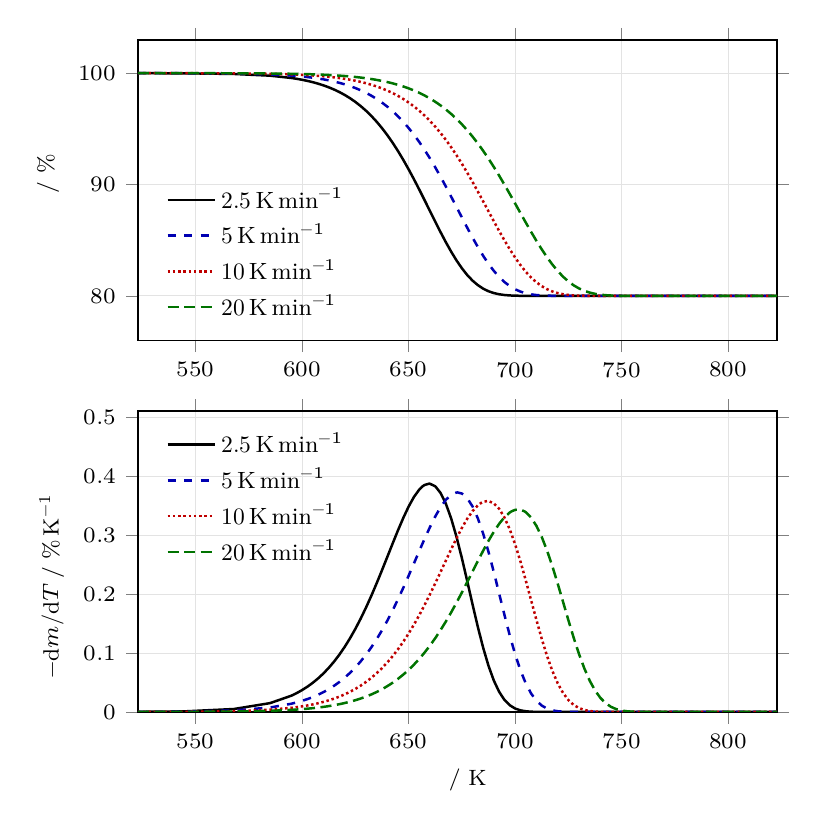
\begin{tikzpicture}
% 图源数据：一级速率方程 d(alpha)/dT=(A/beta)exp(-E/RT)(1-alpha)，alpha(300 K)=0，
% 四条曲线共用 E=180 kJ/mol 与同一个 A，beta=5 K/min 时 Tp=673.000 K；
% TG=100-20alpha，DTG=-dm/dT=20 d(alpha)/dT。下列坐标由
% build/r3/recompute_ch03b_dtg.py 逐点生成（证据见 build/r3/R3-C04-evidence.txt），
% 每一组都含精确峰温节点，所以画出来的峰位就是模型峰位。
\begin{groupplot}[
  group style={group size=1 by 2, vertical sep=9mm},
  xmin=523, xmax=823, xtick={550,600,650,700,750,800},
  tick label style={font={\fontsize{8}{9.6}\selectfont}},
  label style={font={\fontsize{8}{9.6}\selectfont}},
  legend style={font={\fontsize{7.5}{9}\selectfont}, draw=none, fill=none,
                cells={anchor=west}},
  grid=major, major grid style={draw=gray!22, line width=0.3pt},
  every axis plot/.append style={line width=0.9pt},
]
\nextgroupplot[width=\onecolwidth, height=5.4cm,
  ylabel={残余质量 / \%}, ymin=76, ymax=103, ytick={80,90,100},
  legend pos=south west, xticklabel pos=lower]
% TG : beta = 2.5 K/min, Tp = 659.611 K
\addplot[black] coordinates{%
(523,99.9977) (545,99.9869) (568,99.9293) (585,99.7740) (595,99.5672) (597.5,99.4929)
(600,99.4068) (602.5,99.3071) (605,99.1921) (607.5,99.0596) (610,98.9073) (612.5,98.7327)
(615,98.5331) (617.5,98.3053) (620,98.0463) (622.5,97.7526) (625,97.4209) (627.5,97.0475)
(630,96.6289) (632.5,96.1618) (635,95.6432) (637.5,95.0704) (640,94.4416) (642.5,93.7560)
(645,93.0140) (647.5,92.2176) (650,91.3705) (652.5,90.4787) (655,89.5506) (656.611,88.9381)
(657.5,88.5968) (659.611,87.7810) (660,87.6304) (662.5,86.6667) (662.611,86.6242) (665,85.7224)
(667.5,84.8152) (670,83.9624) (672.5,83.1803) (675,82.4822) (677.5,81.8777) (680,81.3716)
(682.5,80.9637) (685,80.6482) (687.5,80.4154) (690,80.2522) (692.5,80.1442) (695,80.0771)
(697.5,80.0383) (700,80.0175) (702.5,80.0073) (705,80.0028) (707.5,80.0009) (710,80.0003)
(712.5,80.0001) (715,80.0000) (717.5,80.0000) (720,80.0000) (722.5,80.0000) (725,80.0000)
(727.5,80.0000) (730,80.0000) (732.5,80.0000) (735,80.0000) (737.5,80.0000) (740,80.0000)
(742.5,80.0000) (745,80.0000) (747.5,80.0000) (750,80.0000) (752.5,80.0000) (755,80.0000)
(757.5,80.0000) (760,80.0000) (762.5,80.0000) (765,80.0000) (767.5,80.0000) (770,80.0000)
(780,80.0000) (795,80.0000) (810,80.0000) (823,80.0000)
};
% TG : beta = 5 K/min, Tp = 673.000 K
\addplot[blue!70!black,dashed] coordinates{%
(523,99.9989) (545,99.9935) (568,99.9646) (585,99.8867) (595,99.7824) (597.5,99.7448)
(600,99.7012) (602.5,99.6505) (605,99.5919) (607.5,99.5241) (610,99.4460) (612.5,99.3560)
(615,99.2526) (617.5,99.1339) (620,98.9980) (622.5,98.8428) (625,98.6660) (627.5,98.4648)
(630,98.2367) (632.5,97.9788) (635,97.6879) (637.5,97.3611) (640,96.9951) (642.5,96.5868)
(645,96.1332) (647.5,95.6317) (650,95.0801) (652.5,94.4767) (655,93.8207) (657.5,93.1124)
(660,92.3535) (662.5,91.5470) (665,90.6980) (667.5,89.8134) (670,88.9022) (672.5,87.9753)
(673,87.7892) (675,87.0458) (676,86.6764) (677.5,86.1281) (680,85.2376) (682.5,84.3901)
(685,83.6006) (687.5,82.8824) (690,82.2460) (692.5,81.6983) (695,81.2420) (697.5,80.8752)
(700,80.5919) (702.5,80.3824) (705,80.2348) (707.5,80.1364) (710,80.0744) (712.5,80.0379)
(715,80.0179) (717.5,80.0078) (720,80.0031) (722.5,80.0011) (725,80.0004) (727.5,80.0001)
(730,80.0000) (732.5,80.0000) (735,80.0000) (737.5,80.0000) (740,80.0000) (742.5,80.0000)
(745,80.0000) (747.5,80.0000) (750,80.0000) (752.5,80.0000) (755,80.0000) (757.5,80.0000)
(760,80.0000) (762.5,80.0000) (765,80.0000) (767.5,80.0000) (770,80.0000) (780,80.0000)
(795,80.0000) (810,80.0000) (823,80.0000)
};
% TG : beta = 10 K/min, Tp = 686.927 K
\addplot[red!75!black,densely dotted] coordinates{%
(523,99.9994) (545,99.9967) (568,99.9823) (585,99.9433) (595,99.8909) (597.5,99.8720)
(600,99.8500) (602.5,99.8245) (605,99.7949) (607.5,99.7606) (610,99.7211) (612.5,99.6754)
(615,99.6227) (617.5,99.5622) (620,99.4926) (622.5,99.4128) (625,99.3215) (627.5,99.2171)
(630,99.0980) (632.5,98.9625) (635,98.8085) (637.5,98.6339) (640,98.4364) (642.5,98.2136)
(645,97.9629) (647.5,97.6815) (650,97.3667) (652.5,97.0157) (655,96.6257) (657.5,96.1941)
(660,95.7185) (662.5,95.1967) (665,94.6274) (667.5,94.0096) (670,93.3433) (672.5,92.6296)
(675,91.8708) (677.5,91.0707) (680,90.2349) (682.5,89.3703) (683.927,88.8673) (685,88.4860)
(686.927,87.7976) (687.5,87.5926) (689.927,86.7280) (690,86.7022) (692.5,85.8280) (695,84.9840)
(697.5,84.1838) (700,83.4405) (702.5,82.7654) (705,82.1672) (707.5,81.6514) (710,81.2200)
(712.5,80.8708) (715,80.5985) (717.5,80.3944) (720,80.2482) (722.5,80.1484) (725,80.0839)
(727.5,80.0446) (730,80.0221) (732.5,80.0102) (735,80.0043) (737.5,80.0017) (740,80.0006)
(742.5,80.0002) (745,80.0001) (747.5,80.0000) (750,80.0000) (752.5,80.0000) (755,80.0000)
(757.5,80.0000) (760,80.0000) (762.5,80.0000) (765,80.0000) (767.5,80.0000) (770,80.0000)
(780,80.0000) (795,80.0000) (810,80.0000) (823,80.0000)
};
% TG : beta = 20 K/min, Tp = 701.424 K
\addplot[green!45!black,dash pattern=on 4pt off 2pt] coordinates{%
(523,99.9997) (545,99.9984) (568,99.9911) (585,99.9716) (595,99.9454) (597.5,99.9359)
(600,99.9249) (602.5,99.9120) (605,99.8972) (607.5,99.8800) (610,99.8600) (612.5,99.8370)
(615,99.8105) (617.5,99.7799) (620,99.7447) (622.5,99.7042) (625,99.6578) (627.5,99.6046)
(630,99.5438) (632.5,99.4743) (635,99.3951) (637.5,99.3049) (640,99.2023) (642.5,99.0859)
(645,98.9541) (647.5,98.8050) (650,98.6369) (652.5,98.4476) (655,98.2350) (657.5,97.9967)
(660,97.7305) (662.5,97.4337) (665,97.1040) (667.5,96.7389) (670,96.3360) (672.5,95.8931)
(675,95.4083) (677.5,94.8800) (680,94.3073) (682.5,93.6896) (685,93.0277) (687.5,92.3228)
(690,91.5777) (692.5,90.7963) (695,89.9840) (697.5,89.1475) (698.424,88.8338) (700,88.2952)
(701.424,87.8064) (702.5,87.4370) (704.424,86.7791) (705,86.5836) (707.5,85.7471) (710,84.9396)
(712.5,84.1733) (715,83.4597) (717.5,82.8086) (720,82.2280) (722.5,81.7229) (725,81.2955)
(727.5,80.9444) (730,80.6654) (732.5,80.4516) (735,80.2942) (737.5,80.1832) (740,80.1085)
(742.5,80.0609) (745,80.0322) (747.5,80.0159) (750,80.0074) (752.5,80.0031) (755,80.0012)
(757.5,80.0004) (760,80.0001) (762.5,80.0000) (765,80.0000) (767.5,80.0000) (770,80.0000)
(780,80.0000) (795,80.0000) (810,80.0000) (823,80.0000)
};
\legend{\qty{2.5}{K.min^{-1}}, \qty{5}{K.min^{-1}},
        \qty{10}{K.min^{-1}}, \qty{20}{K.min^{-1}}}
\nextgroupplot[width=\onecolwidth, height=5.4cm,
  xlabel={温度 / K},
  ylabel={$-\mathrm{d}m/\mathrm{d}T$ / \%\,K$^{-1}$（正峰表示失重）},
  ymin=0, ymax=0.51, ytick={0,0.1,0.2,0.3,0.4,0.5}, legend pos=north west]
% DTG : beta = 2.5 K/min, Tp = 659.611 K
\addplot[black] coordinates{%
(523,0.00019) (545,0.00100) (568,0.00498) (585,0.01496) (595,0.02758) (597.5,0.03199)
(600,0.03704) (602.5,0.04280) (605,0.04936) (607.5,0.05679) (610,0.06520) (612.5,0.07466)
(615,0.08528) (617.5,0.09714) (620,0.11030) (622.5,0.12484) (625,0.14079) (627.5,0.15816)
(630,0.17692) (632.5,0.19696) (635,0.21814) (637.5,0.24022) (640,0.26285) (642.5,0.28559)
(645,0.30788) (647.5,0.32903) (650,0.34824) (652.5,0.36461) (655,0.37718) (656.611,0.38281)
(657.5,0.38498) (659.611,0.38717) (660,0.38709) (662.5,0.38277) (662.611,0.38241) (665,0.37149)
(667.5,0.35313) (670,0.32798) (672.5,0.29684) (675,0.26101) (677.5,0.22225) (680,0.18260)
(682.5,0.14415) (685,0.10887) (687.5,0.07826) (690,0.05326) (692.5,0.03411) (695,0.02041)
(697.5,0.01133) (700,0.00579) (702.5,0.00270) (705,0.00114) (707.5,0.00043) (710,0.00014)
(712.5,0.00004) (715,0.00001) (717.5,0.00000) (720,0.00000) (722.5,0.00000) (725,0.00000)
(727.5,0.00000) (730,0.00000) (732.5,0.00000) (735,0.00000) (737.5,0.00000) (740,0.00000)
(742.5,0.00000) (745,0.00000) (747.5,0.00000) (750,0.00000) (752.5,0.00000) (755,0.00000)
(757.5,0.00000) (760,0.00000) (762.5,0.00000) (765,0.00000) (767.5,0.00000) (770,0.00000)
(780,0.00000) (795,0.00000) (810,0.00000) (823,0.00000)
};
% DTG : beta = 5 K/min, Tp = 673.000 K
\addplot[blue!70!black,dashed] coordinates{%
(523,0.00009) (545,0.00050) (568,0.00250) (585,0.00752) (595,0.01394) (597.5,0.01620)
(600,0.01880) (602.5,0.02178) (605,0.02519) (607.5,0.02909) (610,0.03353) (612.5,0.03857)
(615,0.04430) (617.5,0.05077) (620,0.05806) (622.5,0.06625) (625,0.07543) (627.5,0.08566)
(630,0.09701) (632.5,0.10955) (635,0.12333) (637.5,0.13837) (640,0.15466) (642.5,0.17218)
(645,0.19084) (647.5,0.21049) (650,0.23093) (652.5,0.25186) (655,0.27291) (657.5,0.29360)
(660,0.31335) (662.5,0.33148) (665,0.34725) (667.5,0.35985) (670,0.36843) (672.5,0.37219)
(673,0.37231) (675,0.37045) (676,0.36809) (677.5,0.36268) (680,0.34862) (682.5,0.32836)
(685,0.30236) (687.5,0.27152) (690,0.23714) (692.5,0.20082) (695,0.16434) (697.5,0.12949)
(700,0.09783) (702.5,0.07056) (705,0.04834) (707.5,0.03129) (710,0.01902) (712.5,0.01078)
(715,0.00566) (717.5,0.00273) (720,0.00120) (722.5,0.00048) (725,0.00017) (727.5,0.00005)
(730,0.00001) (732.5,0.00000) (735,0.00000) (737.5,0.00000) (740,0.00000) (742.5,0.00000)
(745,0.00000) (747.5,0.00000) (750,0.00000) (752.5,0.00000) (755,0.00000) (757.5,0.00000)
(760,0.00000) (762.5,0.00000) (765,0.00000) (767.5,0.00000) (770,0.00000) (780,0.00000)
(795,0.00000) (810,0.00000) (823,0.00000)
};
% DTG : beta = 10 K/min, Tp = 686.927 K
\addplot[red!75!black,densely dotted] coordinates{%
(523,0.00005) (545,0.00025) (568,0.00125) (585,0.00377) (595,0.00701) (597.5,0.00815)
(600,0.00947) (602.5,0.01099) (605,0.01273) (607.5,0.01472) (610,0.01700) (612.5,0.01961)
(615,0.02257) (617.5,0.02595) (620,0.02979) (622.5,0.03413) (625,0.03904) (627.5,0.04457)
(630,0.05080) (632.5,0.05777) (635,0.06557) (637.5,0.07425) (640,0.08389) (642.5,0.09453)
(645,0.10624) (647.5,0.11905) (650,0.13297) (652.5,0.14802) (655,0.16415) (657.5,0.18130)
(660,0.19935) (662.5,0.21813) (665,0.23740) (667.5,0.25686) (670,0.27611) (672.5,0.29470)
(675,0.31207) (677.5,0.32760) (680,0.34062) (682.5,0.35042) (683.927,0.35430) (685,0.35630)
(686.927,0.35775) (687.5,0.35762) (689.927,0.35402) (690,0.35383) (692.5,0.34458) (695,0.32975)
(697.5,0.30950) (700,0.28436) (702.5,0.25515) (705,0.22305) (707.5,0.18944) (710,0.15587)
(712.5,0.12382) (715,0.09463) (717.5,0.06931) (720,0.04843) (722.5,0.03214) (725,0.02015)
(727.5,0.01186) (730,0.00652) (732.5,0.00332) (735,0.00156) (737.5,0.00067) (740,0.00026)
(742.5,0.00009) (745,0.00003) (747.5,0.00001) (750,0.00000) (752.5,0.00000) (755,0.00000)
(757.5,0.00000) (760,0.00000) (762.5,0.00000) (765,0.00000) (767.5,0.00000) (770,0.00000)
(780,0.00000) (795,0.00000) (810,0.00000) (823,0.00000)
};
% DTG : beta = 20 K/min, Tp = 701.424 K
\addplot[green!45!black,dash pattern=on 4pt off 2pt] coordinates{%
(523,0.00002) (545,0.00013) (568,0.00062) (585,0.00189) (595,0.00351) (597.5,0.00409)
(600,0.00475) (602.5,0.00552) (605,0.00640) (607.5,0.00740) (610,0.00856) (612.5,0.00988)
(615,0.01139) (617.5,0.01312) (620,0.01509) (622.5,0.01732) (625,0.01986) (627.5,0.02274)
(630,0.02599) (632.5,0.02967) (635,0.03381) (637.5,0.03846) (640,0.04369) (642.5,0.04953)
(645,0.05605) (647.5,0.06331) (650,0.07135) (652.5,0.08024) (655,0.09002) (657.5,0.10074)
(660,0.11243) (662.5,0.12512) (665,0.13880) (667.5,0.15345) (670,0.16902) (672.5,0.18543)
(675,0.20253) (677.5,0.22016) (680,0.23808) (682.5,0.25598) (685,0.27350) (687.5,0.29021)
(690,0.30561) (692.5,0.31916) (695,0.33028) (697.5,0.33835) (698.424,0.34044) (700,0.34279)
(701.424,0.34350) (702.5,0.34308) (704.424,0.34020) (705,0.33879) (707.5,0.32964) (710,0.31555)
(712.5,0.29670) (715,0.27354) (717.5,0.24677) (720,0.21738) (722.5,0.18653) (725,0.15552)
(727.5,0.12563) (730,0.09801) (732.5,0.07361) (735,0.05302) (737.5,0.03648) (740,0.02387)
(742.5,0.01478) (745,0.00862) (747.5,0.00470) (750,0.00239) (752.5,0.00112) (755,0.00048)
(757.5,0.00019) (760,0.00007) (762.5,0.00002) (765,0.00001) (767.5,0.00000) (770,0.00000)
(780,0.00000) (795,0.00000) (810,0.00000) (823,0.00000)
};
\legend{\qty{2.5}{K.min^{-1}}, \qty{5}{K.min^{-1}},
        \qty{10}{K.min^{-1}}, \qty{20}{K.min^{-1}}}
\end{groupplot}
\end{tikzpicture}
\caption{不同升温速率下 TG 与 DTG 的模型曲线（\modelmark，非原书数据）。
两块面板共用横轴（单位为 K，与式~\eqref{eq:ch03b-kissinger}
式~\eqref{eq:ch03b-dTp} 的 $T_{\mathrm p}\approx\qty{673}{K}$ 同一单位）。
读者应看三件事：(a) 四条 TG 曲线的两个平台都落在 100\% 与 80\%，只有转变
区间随升温速率右移；(b) DTG 峰顶由 659.6 K 移到 701.4 K（即 386.4 \degC{} 到
428.3 \degC），升温速率变化八倍峰温移动 41.8 K，每翻一倍上移 13.4--14.5 K；
(c) 纵轴取实际质量导数 $-\mathrm{d}m/\mathrm{d}T$（正峰表示失重）后，四条 DTG
曲线的峰面积都是 $20$ 个质量百分点，等于 TG 上的失重量，与升温速率无关；
但峰高并不严格相等（依次为 $0.387$、$0.372$、$0.358$、$0.343$
\%\,K$^{-1}$，随升温速率略降），因为峰温升高使 $E/(R\,T_{\mathrm p}^{2})$ 变小。
取归一化转化率导数 $\mathrm{d}\alpha/\mathrm{d}T$ 作图时，峰高改为上列数值的
$5$ 倍（$1.94$、$1.86$、$1.79$、$1.72$ \%\,K$^{-1}$），面积改为 $100\%$，
结论不变；两种口径不能混用。
模型条件：四条曲线由同一条一级速率方程
$\mathrm{d}\alpha/\mathrm{d}T=(A/\beta)\exp[-E/(R\,T)]\,(1-\alpha)$ 积分得到，
固定失重 20\%，共用 $E=\qty{180}{kJ.mol^{-1}}$ 与同一个频率因子 $A$，
峰温由动力学自动给出（$\beta=\qty{5}{K.min^{-1}}$ 时 $T_{\mathrm p}=673.0$ K，
其余三条由同一组参数解出）；按式~\eqref{eq:ch03b-kissinger} 回算这四组峰温
得到的 $E$ 与设定值一致。峰温处的转化率 $\alpha(T_{\mathrm p})\approx0.61$，
所以峰温不能当作半转化温度。温度程序自 300 K 起积分，523 K 处
$\alpha<2\times10^{-4}$，因此两条平台在图上仍读作 100\% 与 80\%。
真实样品的 DTG 峰高一般随升温速率上升（实际失重速率还随 $\beta$ 增大）；
这里用同一坐标作图是为了让「峰面积不变」直接可见。未计入传热滞后、浮力与
基线漂移。
\figsrc{据本章动力学讨论绘制，上册 §3.3，书内 p.181 / PDF p.200。}}
\label{fig:ch03b-rate}
\end{figure}

\begin{example}[读图：升温速率改变的是峰温还是峰面积]
\begin{obs}
在图 \ref{fig:ch03b-rate} 上逐条读出的内容：
(a) 面板中，升温速率从 \qty{2.5}{K.min^{-1}} 增到 \qty{20}{K.min^{-1}} 时，
四条曲线的起始平台都在 100\%，终止平台都在 80\%，转变段的中心依次右移；
(b) 面板中，DTG 峰顶的位置依次为 659.6、673.0、686.9、701.4 K（即 386.4、
399.9、413.8、428.3 \degC），八倍速率之间峰温移动 41.8 K；把这四组峰温按
式~\equref{eq:ch03b-kissinger} 作
$\ln(\beta/T_{\mathrm p}^{2})$--$1/T_{\mathrm p}$ 图，回算得到的 $E$ 就是
生成曲线时设定的 \qty{180}{kJ.mol^{-1}}；
(c) 峰的最大高度（纵轴为实际质量导数 $-\mathrm{d}m/\mathrm{d}T$）依次为
0.387、0.372、0.358、0.343 \%\,K$^{-1}$，随升温速率略降；四个峰的半高宽
依次约为 47、49、51、53 K（约为转变区间宽度的三分之一）。峰温处 TG 的
残余质量为 87.8\%（$\beta=\qty{5}{K.min^{-1}}$），即该处 $\alpha\approx0.61$，
不是一半。
两步之间没有出现新的失重台阶，也没有出现肩峰。
\end{obs}
\begin{infer}
由「两个平台位置相同」推断：这一步的总失重量为 20\%，与升温速率无关，
因此失重量可以作为定量的依据。由「峰顶随升温速率单调右移、且位移量随
$\ln(\beta_2/\beta_1)$ 近似线性」推断：峰温位移来自动力学，不是材料在
不同实验里变成了不同的东西。由「只有一个峰、无肩峰」推断：至少在当前的
分辨能力下，这一步可以按单一过程处理。

不能由本图推断的内容：不能推断该过程的活化能具体是多少——图
\ref{fig:ch03b-rate} 的 $E=\qty{180}{kJ.mol^{-1}}$ 是生成曲线时\emph{设定}的
参数，上一条回算只是自洽性检验，不是对真实样品的测量；真实体系必须用实测
峰温按式~\equref{eq:ch03b-kissinger} 拟合才能得到 $E$；
不能推断样品的热稳定性温度（峰温不是稳定性判据）；也不能排除存在两个
活化能相近、峰位重叠的步骤。
\end{infer}
\end{example}

\begin{dataflow}
从原始曲线到可比的量，四步：

① 扣空白与浮力校正。同一温度程序、同一坩埚、同一流量下先测空坩埚，
从样品曲线中减去；未做这一步，峰位判读本身就不成立。

② 定位。用 DTG 峰顶定 $T_{\mathrm p}$，用平台差定失重量 $\Delta m$，
用 DTG 的起始偏离点与回折点定温度区间。

③ 判别位移来源。把 $T_{\mathrm p}$ 按式 \equref{eq:ch03b-kissinger} 作
$\ln(\beta/T_{\mathrm p}^{2})$ 对 $1/T_{\mathrm p}$ 的图：若成直线，
位移全部来自动力学；若明显偏离直线，说明发生了传热控制或反应路径改变。

④ 定量。用失重量而不是峰高做定量；只在步骤 ①--③ 都通过后才比较不同样品。
\end{dataflow}

\begin{table}[tbp]
\centering
\caption{实验条件对曲线的三种作用：峰温、峰形、峰面积。读者应看出第 3、4 列
的规律——峰温几乎对所有条件敏感，峰面积只对「反应路径改变」与「基线未扣」
敏感。表中「基本不变」指该量为守恒量时的不变性，仍可能被重叠峰拆分误差放大。
\src{据上册 §3.6，书内 p.209—212 / PDF p.228—231 归纳；表中峰温位移量按
Arrhenius 动力学估算，非源书实验数据。}}
\label{tab:ch03b-conditions}
\small
\begin{tabular}{@{}p{42mm}p{28mm}p{28mm}p{38mm}@{}}
\toprule
实验因素（作用机制） & 对峰温 $T_{\mathrm p}$ & 对峰形 & 对峰面积／失重量 \\
\midrule
升温速率 $\beta$ 增大（动力学控制，式 \equref{eq:ch03b-kissinger}） &
显著上移，八倍速率可移 40 K 以上 &
整体向高温展宽，相邻峰更易重叠 &
基本不变 \\
样品量增大（颗粒床内部传热与传质滞后，自生气氛增强） &
上移 &
展宽、拖尾，分辨下降 &
名义不变，但重叠峰拆分误差被放大 \\
气氛改变（惰性转为氧化性） &
可大幅移动，甚至原峰消失、新峰出现 &
峰数改变（出现燃烧峰） &
\textbf{会真正改变}：反应路径不同，失重量不同 \\
载气流量增大（产物分压降低，抑制逆反应） &
略降 &
略变窄 &
一般不变；流量突变会引起假失重或假增重 \\
坩埚材质与形状改变（催化、与样品反应、热导与热容不同） &
改变 &
可能畸变，可出现假峰 &
坩埚参与反应时失真 \\
粒度与堆积改变（大颗粒内部温度梯度，堆积层厚） &
大颗粒、厚堆积时上移 &
展宽 &
基本不变 \\
浮力与基线未扣（气体密度随温度变化） &
表观漂移，峰位判读失真 &
整体倾斜，出现假台阶 &
直接污染，产生假失重或假增重 \\
\bottomrule
\end{tabular}

\vspace{1.5mm}
{\footnotesize 结论：\textbf{峰面积（总失重量、总焓变）是条件相对稳健的量，
峰温是最容易被条件左右的量}。任何「用峰温比较材料稳定性」的结论，都必须
先固定升温速率、样品量、气氛、坩埚与流量这五项。}
\end{table}

\begin{pitfall}
\textbf{把峰温当材料常数。} 由式 \equref{eq:ch03b-dTp}，\qty{5}{K.min^{-1}}
下测得的 \qty{420}{\celsius} 与 \qty{20}{K.min^{-1}} 下测得的
\qty{455}{\celsius} 完全可以是同一种材料。跨文献比较峰温之前，必须先确认
升温速率相同。

\textbf{用 DTG 峰高代替峰面积。} 峰高正比于升温速率（$\mathrm{d}m/\mathrm{d}t
= \beta\,\mathrm{d}m/\mathrm{d}T$），换一个速率峰高就变，峰面积才守恒。
图 \ref{fig:ch03b-rate} 的纵轴取 $-\mathrm{d}m/\mathrm{d}T$ 而不是
$-\mathrm{d}m/\mathrm{d}t$，就是为了让四个速率下的曲线落在同一坐标上比较；
换成 $-\mathrm{d}m/\mathrm{d}t$ 作图，峰高会随 $\beta$ 按比例升高。

\textbf{把肩峰当新相。} 样品量偏大或粒度不均时，同一个过程会因床层温度
分布而裂成主峰加肩峰。判据：把样品量减半，若肩峰消失或大幅减弱，
则它来自传热而非新相。
\end{pitfall}

\begin{crosscheck}
三项回查按顺序做：① 空白基线回查——空坩埚曲线在同一温度区间应当平坦，
若不平坦，先修基线；② 样品量回查——样品量减半后重测，峰温应下移或不变，
若显著上移则原曲线受传热控制；③ 升温速率回查——用两个以上速率重测，
按式 \equref{eq:ch03b-kissinger} 作图，直线性本身就是数据自洽的证据。
三项都通过后，才允许把峰温写进结论，并且必须与升温速率一起写。
\end{crosscheck}

\subsection{气氛：改变的是反应路径，不只是反应速率}

\begin{probout}
气氛不是「背景条件」，而是反应物或产物的一部分。同一样品在空气与氮气下
得到的两条曲线，其失重步数、失重温度区间与失重量都可能不同，因此
\textbf{不可互相比较，也不能互相换算}。本节要回答：如何从曲线形状判断
气氛是否改变了反应路径，以及如何在两种气氛之间建立可比的实验设计。
\end{probout}

\begin{principle}
惰性气氛下发生的是热解、脱羟基、脱碳酸盐一类反应，固相自身分解，
逸出物是分解产物；氧化性气氛下，同样的有机或还原性组分会被氧化，
逸出物是 \ce{CO2} 与 \ce{H2O}，同时释放热量。

这一差别在两类曲线上的表现是互补的：
\begin{itemize}
  \item TG 上，惰性气氛下碳质残留会形成残炭，失重不彻底；空气下残炭被
  氧化烧掉，失重量更大，且多出一个高温失重步。因此\textbf{用空气下的
  失重量测碳含量是可行的，用氮气下的失重量测碳含量则系统性偏低}。
  \item DSC/DTA 上，同一过程在惰性下常表现为吸热（分解需要能量），
  在氧化性下可能表现为放热（燃烧放热）。峰的热效应符号可以直接翻转，
  这是判断「这一步是不是燃烧」最直接的证据。
\end{itemize}
本书中积炭催化剂的 DSC 测试正是用这一判别方法：先在惰性气氛下升温，
切换到氧气后出现一个明显的放热峰，该峰被归因于催化剂表面积炭被氧化成
\ce{CO2}、\ce{CO} 等挥发物；由此得到「积炭覆盖活性中心或堵塞孔道导致
活性下降」的结论。\src{上册 §3.4.1，书内 p.184--185 / PDF p.203--204}
这里读出的是两件事：失重步的出现是质量证据，放热峰的出现是热效应证据，
两者合起来才支持「可燃的碳质物种」这一归属；仅凭其中一个都会过度解读。
\end{principle}

\begin{measure}
气氛条件的五项记录：气体种类与纯度、流量、样品处实际气氛（是否被自身
分解产物改性）、是否中途切换气氛、切换时的温度与稳定时间。

三个容易被忽略的实际问题：
\begin{itemize}
  \item \textbf{残余氧。} 高纯氮中若含氧量偏高，碳的氧化峰依然会出现，
  但位置和形状与空气下不同，容易误判为「材料本身的低温氧化」。
  怀疑时用氩气复测或检测尾气含氧量。
  \item \textbf{自生气氛。} 样品量偏大时，分解产物在床层内累积，
  使样品实际处于还原性或产物富集的气氛中，与名义气氛不同。
  这是样品量与气氛两个变量的耦合，减小样品量即可验证。
  \item \textbf{气体的热导率影响 DSC 基线。} 切换气氛会改变基线，
  所以两种气氛下的曲线必须各自做各自的空白基线，不能共用。
\end{itemize}
\tocheck{未对照原页面图像：本段的残余氧与自生气氛讨论为学科通用实践，
源 OCR 未展开；切换气氛的实例见书内 p.184--185 的 DSC 测试描述。}
\end{measure}

\begin{dataflow}
判断「气氛是否改变了反应路径」的四步：

① 在惰性气氛与空气下各做一次，其余条件（速率、样品量、坩埚、流量）完全相同；

② 比较失重步数：空气下多出的失重步通常是可燃组分的氧化；

③ 比较热效应符号：惰性下吸热、氧化下放热的同温区过程，基本可以判定为
氧化反应；

④ 比较总失重量：若两者差值与残炭量相当，则「惰性下残炭、空气下烧尽」
的解释成立；若差值与残炭量不符，说明还有别的路径，需要逸出物分析。
\end{dataflow}

\begin{pitfall}
\textbf{跨气氛比较特征温度。} 把文献中氮气下的分解温度与本实验室空气下的
起始氧化温度并列，得到的「稳定性对比」没有意义：空气下测的是氧化起始温度，
氮气下测的是热分解温度，两者不属于同一个过程。

\textbf{把气氛效应当催化效应。} 掺杂样品在空气下氧化温度降低，可能只是
掺杂提高了氧的传输或增加了比表面积，而不是催化了分解本身。区分方法是
在惰性气氛下重测同一对样品：若惰性下的峰温不降，则空气下的降低属于氧化
路径的促进。

\textbf{忘记气氛流量对峰温的次级影响。} 流量增大使产物分压降低，
对可逆分解过程会略微降低峰温。在同一气氛内比较不同样品时影响不大，
但把「流量不同的两组数据」当作「气氛不同的两组数据」来解读则会出错。
\end{pitfall}

\begin{crosscheck}
气氛结论至少需要一项非热分析证据：元素分析（CHN）给出碳含量、
XRD 给出固相物相、尾气分析给出逸出物组成。对积炭一类问题，
「空气下的失重增量」应当与元素分析测得的碳含量在误差范围内一致。
本书中 \ce{CuO}-\ce{ZnO}-\ce{Al2O3}-\ce{CrO_x} 前驱体组成的确定，
用的就是这种质量平衡回查（见下节实例），只是那里的对照对象是
按化学计量计算的理论失重。
\end{crosscheck}

\subsection{五类典型误判与回查方法}

\begin{probout}
本节把热分析中最常见、也最容易写进论文结论的五类误判集中列出，
每一条都给出「误判长什么样」与「用什么实验回查」。这一节的用法不是通读，
而是在得到一条反常结论时逐条对照。
\end{probout}

\begin{principle}
五类误判有一个共同的根源：把\textbf{峰温}当成了材料的固有属性。
峰温由动力学与传热共同决定（式 \equref{eq:ch03b-kissinger}、
式 \equref{eq:ch03b-dTp}），只有峰面积与失重量属于守恒量。凡是从峰位
出发的结论，都需要额外证据；凡是从峰面积出发的结论，只需要确认基线正确
与过程单一。
\end{principle}

\begin{pitfall}
\textbf{（一）把峰温位移当材料稳定性差异。} 两组样品的 DTG 峰温相差 30 K，
结论写成「B 比 A 稳定」。真实原因常常只是两次实验的升温速率不同
（\qty{5}{K.min^{-1}} 对 \qty{10}{K.min^{-1}}），或样品量相差一倍。

\emph{回查}：固定升温速率重测；或对每个样品各取四个升温速率，
按式 \equref{eq:ch03b-kissinger} 求 $E$，用 $E$ 而不是 $T_{\mathrm p}$
比较稳定性。本书中 12-钨硅酸负载到 HEMT 沸石后分解放热峰由
\qty{522.12}{\celsius} 移到 \qty{559.13}{\celsius}，
结论是「二者之间发生了相互作用」，这一比较之所以成立，
是因为两条件在同一升温速率下测得。\src{上册 §3.4.1，
书内 p.183--184 / PDF p.202--203} 反过来，如果这两个数字来自不同的
升温速率，则该结论不成立。

\textbf{（二）基线未扣或浮力未校正。} 表现为低温段缓慢漂移、高温段整体
倾斜，或出现一个「谁也没见过」的宽失重台阶。浮力随温度升高使表观质量
单调变化，其大小与升温速率和气体种类都有关，常被误读为「表面吸附水的
连续脱除」。

\emph{回查}：同一条件下测空坩埚，用同一程序做空白并相减；
再把载气由氮气换成氩气，真正的样品失重不变，浮力引起的漂移会变。

\textbf{（三）坩埚与样品反应。} 坩埚不是惰性容器。碱金属或碱土金属的
碳酸盐、硫酸盐在高温下可与氧化铝或石英坩埚反应；铂坩埚对有机物的
氧化有催化作用，也可能与某些金属形成合金；镍、铁一类样品在高温下
与氧化铝坩埚发生界面反应。表现是峰温偏移、出现附加峰，
严重时失重量也失真。

\emph{回查}：换一种材质的坩埚（如氧化铝换铂或换石墨）重测同一份样品。
若曲线不变，坩埚惰性成立；若曲线改变，先前所有定量结论都需要重做。
\tocheck{未对照原页面图像：坩埚与样品反应的具体体系为学科通用认识，
源 OCR 未列出实例，待与本实验室规程核对。}

\textbf{（四）样品量过大致传热滞后。} 床层内部存在温度梯度，
热电偶测的是坩埚附近的温度而不是样品中心的温度，于是样品实际温度低于
记录温度，曲线向高温方向整体平移并展宽。表现是峰温偏高、相邻峰合并、
肩峰出现。对动力学分析而言，这会把表观活化能算小。

\emph{回查}：样品量减半（必要时再减半）重测。若峰温下移且峰变窄，
说明原曲线受传热控制，应取小样品量的数据；若峰温不变，样品量不是变量。

\textbf{（五）用 TG 失重直接推断物种而不做逸出物分析。}
失重 18\% 就被写成「失去两个结晶水」，失重 6\% 就被写成「脱除结构羟基」。
数值巧合不能作为物证：不同的物种组合可以给出同一个失重量，
同一步失重也可能同时包含多个物种。

\emph{回查}：三件事至少做一件——按化学计量计算\textbf{理论失重}并与实测比较；
用联用技术做逸出物分析；用 XRD 或元素分析确认终态固相。
本书中前驱体组成的确定正是这一思路的正例：先按可能的沉淀物组成算出理论
分解失重，与实测值比较，发现理论值系统性大于实测值且偏差较大，
据此判断沉淀物的设计有问题；改用铬酸钠作铬源重新设计沉淀反应后，
理论失重与实测失重的偏差缩小到 \qty{0.9}{\percent} 以内，
才确认新组成正确。\src{上册 §3.4.1，书内 p.186--188 / PDF p.205--207}
这里 TG 的作用是\emph{验证}组成假设，不是\emph{发现}组成。

另一个反例是球磨 \ce{Al}-\ce{SnCl2} 复合物的 DSC 测试：第一次升温出现两个
吸热峰，第二次升温第一个峰消失、第二个峰保留，说明前者不可逆、后者可逆；
可逆峰的起始点 \qty{225.2}{\celsius} 与纯锡熔点 \qty{230}{\celsius} 接近，
不可逆峰的起始点 \qty{180.9}{\celsius} 与 \ce{AlCl3} 升华温度
\qty{183}{\celsius} 接近。若只看 DSC 曲线本身，这两个峰最多只能说成
「某物熔化／升华」；只有把 XRD 检出新相金属锡、EDS 检出氯元素分布，
才能写成「\ce{Sn^2+} 被还原为金属锡并生成 \ce{AlCl3}」。
\src{上册 §3.4.4，书内 p.195--196 / PDF p.214--215}
\end{pitfall}

\begin{crosscheck}
把五条回查整理成一张可执行的清单：

\begin{itemize}
  \item 峰位类结论 → 用「固定升温速率重测」+「Kissinger 图直线性」回查；
  \item 失重量类结论 → 用「空白基线」+「理论化学计量失重」回查；
  \item 物种归属类结论 → 用「逸出物分析」+「XRD／元素分析」回查；
  \item 稳定性类结论 → 用「多个升温速率」+「同一样品量」回查；
  \item 催化效应类结论 → 用「惰性与氧化两种气氛」回查。
\end{itemize}

五条中最容易被跳过的是第一条。建议在实验记录模板里把升温速率与样品量
写成与样品名称并列的必填字段，从流程上消除这个误判。
\end{crosscheck}

\subsection{应用实例选读：从曲线到结论}

\begin{probout}
本节按「观测—推断—回查」三段式读四个实例，覆盖本书第 3 章应用部分的主要
类型：焙烧温度的确定、负载后峰温位移的解读、前驱体组成的质量平衡验证、
以及由峰温求脱氢活化能。读这些实例的重点不是记住结论，
而是看清每条结论背后必须有的独立证据。
\end{probout}

\subsubsection{焙烧温度的确定：热分析与 XRD 的互补}

\begin{dataflow}
\textbf{观测。} 含铜、锌、镍硝酸盐的沉淀混合物经干燥后进行 DTA-TG 测试
（\src{上册 §3.4.1，书内 p.182 / PDF p.201}）：\qty{180}{\celsius} 以前有
少量失重；\qty{180}{\celsius}--\qty{420}{\celsius} 之间 DTA 出现明显峰，
同时 TG 上有较大失重；温度达到 \qty{400}{\celsius} 以上，TG 与 DTA 曲线
都接近直线。

\textbf{推断。} 低温段少量失重归因于表面水分的脱除；中温段的
「DTA 峰 + TG 失重」同时出现在同一温区，说明该区间发生了沉淀物的分解；
\qty{400}{\celsius} 以上两条曲线都变平，说明分解已经完成，
故焙烧温度应取 \qty{400}{\celsius} 左右。

\textbf{回查。} 在 \qty{320}{\celsius}、\qty{400}{\celsius}、
\qty{500}{\celsius} 三个温度下焙烧后做 XRD：\qty{320}{\celsius} 时物相
基本为非晶型，衍射峰不明显；\qty{400}{\celsius} 时几种氧化物的衍射峰较为
明显；\qty{500}{\celsius} 时衍射结果与 \qty{400}{\celsius} 几乎相同，
但温度过高易出现烧结，影响比表面积与强度。综合两者，最佳焙烧温度定在
\qty{400}{\celsius} 左右。\src{上册 §3.4.1，书内 p.183 / PDF p.202}

这里的分工值得注意：热分析指出「分解在哪个温区完成」，
XRD 指出「分解后是否形成了需要的物相」。二者缺一，
「\qty{400}{\celsius} 最佳」这个结论都不完整——单看 TG 只能说分解完成，
单看 XRD 只能说物相出现，都没有给出温度下限与上限的组合判据。
\end{dataflow}

\subsubsection{负载后峰温向高温移动：相互作用还是实验条件}

\begin{dataflow}
\textbf{观测。} HEMT 沸石样品仅在 \qty{100}{\celsius} 附近出现一个脱水峰；
12-钨硅酸本身有三个峰，\qty{61.3}{\celsius} 与 \qty{191.4}{\celsius} 两个
吸热峰分别对应失去结晶水与结构水，\qty{522.12}{\celsius} 的放热峰对应
杂多酸结构的分解。HEMT 负载约三分之一杂多酸后，在 \qty{559.13}{\celsius}
出现一个小的放热峰。\src{上册 §3.4.1，书内 p.183--184 / PDF p.202--203}

\textbf{推断。} 该放热峰与 12-钨硅酸的分解峰对应，但峰位向高温方向移动，
说明负载到 HEMT 表面后杂多酸与载体之间发生了相互作用，
使其分解需要更高的温度。

\textbf{边界。} 这一推断成立的前提是两次测试的升温速率相同。
若升温速率不同，按式 \equref{eq:ch03b-dTp}，八倍速率差即可造成 40 K 以上的
峰温位移，恰好覆盖本例中 37 K 的位移量，结论就会完全反转。
因此这类比较必须在实验部分明确写出升温速率，并在图中标注。源 OCR 未给出
该实验的升温速率，此处不能替它补齐。\tocheck{未对照原页面图像：
图 3-12 的升温速率在 OCR 文本中缺失，本例的峰温可比性依赖这一条件。}
\end{dataflow}

\subsubsection{前驱体组成：用理论失重做质量平衡验证}

\begin{dataflow}
\textbf{观测。} 按投料比设计的 \ce{CuO}-\ce{ZnO}-\ce{Al2O3}-\ce{CrO_x}
催化剂前驱体，在空气下测得的 DTG 曲线呈「双馒头峰」，分解温区约为
\qty{140}{\celsius}--\qty{360}{\celsius}，到 \qty{450}{\celsius} 结束；
按沉淀物组成计算的理论热分解失重与实测失重相比，理论值均大于实测值，
偏差较大。\src{上册 §3.4.1，书内 p.185--186 / PDF p.204--205}

\textbf{推断。} 理论失重与实测失重的系统性偏差，说明所假定的沉淀物组成
不对，即前驱体的沉淀物设计有问题。

\textbf{回查。} 分别制备以 \ce{Na2CO3} 为沉淀剂和以 \ce{Na2CrO4}（铬酸钠）
为铬源的 \ce{CuO}-\ce{Al2O3} 前驱体并比较其 DTG：前者是一个尖锐的峰，
主要来自碳酸铜类沉淀的分解；后者出现的是另一个特征的峰。
据此判断，\ce{CuO}-\ce{ZnO}-\ce{Al2O3}-\ce{CrO_x} 前驱体的双馒头峰与
铬酸钠参与沉淀有关，即铬酸钠使碳酸铜不能生成或只生成氢氧化铜。
按新组成重新计算理论失重后，与实测值的偏差缩小到 \qty{0.9}{\percent}
以内（\src{上册 §3.4.1，书内 p.187--188 / PDF p.206--207}），
从而确认后一种沉淀物种的设计是正确的，并进一步说明：
以铬酸钠作铬源引入时会与硝酸铜生成铬酸铜沉淀，同时抑制碳酸铜的生成。
\end{dataflow}

\begin{pitfall}
本例是整个应用部分最容易被误读的一处。TG 曲线本身只给出「失了多少」，
它无法直接说出「失去的是什么」。这里之所以能判断组成，
是因为用了\textbf{两个独立的约束}：一是理论化学计量失重，
二是不同沉淀剂条件下 DTG 峰形的差异。如果把「双馒头峰」直接读成
「两种碳酸盐分解」，就跳过了全部验证步骤，属于上文第（五）类误判。
\end{pitfall}

\subsubsection{由峰温求脱氢活化能：峰温位移的正确用法}

\begin{dataflow}
\textbf{观测。} 对球磨处理及掺杂不同尺度 \ce{TiH2} 的 \ce{LiAlH4} 样品做
非等温脱氢的 TGA 与 DSC 测试，得到两步脱氢过程。由不同升温速率下的 DSC
峰温，按动力学方法算得两步脱氢的表观活化能：球磨样品为
\qty{96.0}{kJ.mol^{-1}} 与 \qty{92.7}{kJ.mol^{-1}}；
掺入微米级 \ce{TiH2} 后降为 \qty{82.9}{kJ.mol^{-1}} 与
\qty{82.5}{kJ.mol^{-1}}；掺入纳米级 \ce{TiH2} 后进一步降为
\qty{76.1}{kJ.mol^{-1}} 与 \qty{68.5}{kJ.mol^{-1}}。
\src{上册 §3.4.4，书内 p.196--197 / PDF p.215--216}
\tocheck{未对照原页面图像：上列活化能数值取自表 3-11 的 OCR 文本，
其中个别数字的末位存在识别风险，数值本身仅供量级判断。}

\textbf{推断。} 掺杂使两步脱氢的表观活化能同时降低，且纳米级 \ce{TiH2}
的降低幅度更大，因此纳米级 \ce{TiH2} 对 \ce{LiAlH4} 脱氢的催化效果更好；
这与 TGA 上观测到的起始脱氢温度下降一致。

\textbf{为什么这里可以用峰温。} 与上一节「不能直接用峰温比较稳定性」并不
矛盾：这里不是在比较两个温度数字，而是把\textbf{同一样品在多个升温速率下}
的峰温整体作为输入，用动力学关系提取出一个条件无关的量——活化能。
峰温在这里是中间量，不是结论。这正是误判第（一）条给出的正确做法。
\end{dataflow}

\begin{crosscheck}
四个实例的共同结构：热分析给出温度区间与质量／热效应变化，
另外一项独立测量（XRD、元素分析、理论化学计量、多速率动力学分析）
给出归属或守恒量，两者都成立才写结论。

对本节内容做回查时按下列顺序：先确认升温速率与样品量已记录，
再确认基线已扣，然后确认失重步与理论化学计量或逸出物分析对得上，
最后才检查峰位类结论是否有多速率支持。四项中任一缺失，
相应结论都应当降级为「现象描述」。

\srcnote{本节实例分别取自上册 §3.4.1（书内 p.182--189 / PDF p.201--208）、
§3.4.4（书内 p.194--198 / PDF p.213--217）。联用技术对照表与实验条件
影响表中的接口参数、量级范围为学科通用认识整理，源 OCR 未给明文；
正文中所有 \tocheck{} 项待与原页面图像逐条核对。}
\end{crosscheck}
}{}
\IfFileExists{chapters/parts/ch03-c.tex}{\input{chapters/parts/ch03-c}}{}
\IfFileExists{chapters/parts/ch03-d.tex}{\input{chapters/parts/ch03-d}}{}
\IfFileExists{chapters/parts/ch03-e.tex}{\input{chapters/parts/ch03-e}}{}
}{}
\IfFileExists{chapters/ch04.tex}{% chapters/ch04.tex —— 第 4 章 多晶X射线衍射分析
% 装配层：只负责按顺序引入各分片。分片缺失时跳过，便于增量成书。
% 分片文件：chapters/parts/ch04-{a..e}.tex

\IfFileExists{chapters/parts/ch04-a.tex}{% ================================================================
%  chapters/parts/ch04-a.tex
%  第 4 章  多晶 X 射线衍射分析（分片 a）
%  源：S1（上册）第 4 章，书内 p.219—243 / PDF p.238—262
%  覆盖：4.1 晶体学基础：周期性与对称性
%        4.2 X 射线的性质及其与物质的作用
%        4.3 衍射的几何原理：倒易空间与衍射方法
%  状态：分片 a（4.4 及以后由分片 b/c 续写）
% ================================================================

\chapterstart{多晶X 射线衍射分析}%
{本章回答：一张多晶衍射图上的\textbf{峰位、峰强、峰形}各自编码了晶体结构的哪一部分信息，
它们分别需要什么条件才能被可靠读出，以及哪些结论单靠衍射数据无法支撑。分片 a 建立三块
共用基础：晶体学的周期性与对称性（4.1）、X 射线的产生及其与物质的相互作用（4.2）、
以倒易格子和 Ewald 球表述的衍射几何（4.3）。后续分片在此基础上讨论物相鉴定、定量、
指标化与 Rietveld 精修。}
\label{ch:04}

\subsection{晶体学基础：周期性与对称性}

\begin{probout}
多晶衍射测量的对象是\textbf{大量无规取向微晶的集合}。与单晶衍射相比，它把三维倒易空间
的数据压缩成以晶面间距 $d$ 为变量的一维数据：$d$ 值相同的衍射完全重合，$d$ 值相近的
衍射相互重叠。因此一张多晶图上可\textbf{直接}读出的只有三件事——\textbf{峰位}、
\textbf{峰强}和\textbf{峰形}；其余信息（物相、晶胞参数、晶粒尺寸、微应变、甚至原子坐标）
都是在这三个量上做反演得到的，反演的可靠性取决于对晶体学与衍射几何的掌握程度。
\end{probout}

这一节只讲三件与衍射直接挂钩的事：\textbf{周期性}（决定衍射是否出现）、
\textbf{对称性}（决定衍射如何系统性缺席）、\textbf{晶面与衍射指标}（决定如何给一个峰
命名）。纯群论内容在此压缩为一张表，把篇幅让给后面的主线。

\subsubsection{晶体的空间点阵与周期性}

晶体的定义性特征是\textbf{结构基元在三维空间中周期性重复}。把每个重复单元抽象成一个
几何点，这些点构成的无限周期排列即\textbf{空间点阵}；点阵中任意两点之差都属于平移群
\begin{equation}
T=m\boldsymbol{a}+n\boldsymbol{b}+p\boldsymbol{c},
\qquad m,\,n,\,p=0,\pm1,\pm2,\dots
\label{eq:transgroup}
\end{equation}
其中 $\boldsymbol{a},\boldsymbol{b},\boldsymbol{c}$ 是三个互不平行的基矢。式~\eqref{eq:transgroup}
的成立条件是\textbf{结构严格周期}且\textbf{忽略表面与缺陷}：真实晶体尺寸远大于重复周期，
故可近似视为向三维无限延伸。量纲检查：$m,n,p$ 为纯数，$\boldsymbol{a},\boldsymbol{b},
\boldsymbol{c}$ 为长度，故 $T$ 为长度向量，与「平移」的物理含义一致。

\begin{example}[萤石晶胞的重复单元数]
\ce{CaF2} 属立方晶系，晶胞参数 $a=\qty{5.462}{\angstrom}$，每个晶胞含 4 个 \ce{Ca^2+}
和 8 个 \ce{F^-}。由 $V=a^{3}\approx\qty{1.63e-1}{nm^3}$，可估算
$\qty{1}{mm^3}$ 晶体中约有 $10^{19}$ 个这样的重复单元。这个数量级说明：多晶样品中
「参与衍射的晶胞数极大」，这正是后文把干涉近似处理为\textbf{严格满足条件才出峰}、
否则完全相消的根据。
\end{example}

\subsubsection{对称性：从对称要素到点群与空间群（压缩表）}

\textbf{对称操作}是能使物体复原的动作，其所凭借的几何元素（点、线、面）称\textbf{对称要素}；
全部对称操作的集合构成\textbf{对称操作群}，群中操作的数目称\textbf{阶次}。晶体中可能的
对称操作包括旋转（$L$）、反映（$m$）、倒反（$i$）、旋转倒反（反轴）及其联合操作。
受点阵平移性质的限制，\textbf{晶体中只存在 1、2、3、4、6 次轴}，不存在五次轴与高于
六次的轴；宏观对称要素的组合必交于一点。由第一类操作（旋转）构成的点群 11 个，与第二类
操作组合后共得 \textbf{32 种点群}；加入平移型要素（螺旋轴、滑移面）后得
\textbf{230 种空间群}。X 射线衍射中，在反常散射不严重时衍射数据自带对称中心，故由衍射
数据构建的点阵中只有 \textbf{11 种 Laue 群}。

表~\ref{tab:crystal-systems} 把七个晶系、14 种布拉维点阵型式、点群与特征对称元素压缩在
一张表内\src{S1 §4.1.2，书内 p.225—228 / PDF p.244—247}。使用这张表时有两个方向性区别
必须记牢。

\begin{table}[htbp]
\centering
\caption{七个晶系、布拉维点阵型式与特征对称元素（压缩表）\src{据 S1（上册）表 4-2、图 4-3，书内 p.226—227 / PDF p.245—246 整理。}}
\label{tab:crystal-systems}
{\srcsize
% 原为 @{}lXX@{}：首列 l 吃掉自然宽度，两个 X 列被挤到低于最小内容宽度（36.0 pt overfull）。
% 改为定宽 p{24mm}，首列可折行，宽度留给 X 列。
\begin{tabularx}{\columnwidth}{@{}>{\raggedright\arraybackslash}p{24mm}XX@{}}
\toprule
晶系 & 晶胞参数与点阵型式 & 特征对称元素（点群） \\
\midrule
三斜 & $a\neq b\neq c$，$\alpha\neq\beta\neq\gamma$；$aP$ & 无（$C_1$，$C_i$） \\
单斜 & $a\neq b\neq c$，$\alpha=\gamma=90^{\circ}\neq\beta$；$mP$、$mC$ & 1 个对称面或 1 个二次轴（$C_2$，$C_s$，$C_{2h}$） \\
正交 & $a\neq b\neq c$，$\alpha=\beta=\gamma=90^{\circ}$；$oP$、$oI$、$oC$、$oF$ & 2 个互相垂直的对称面或 3 个互相垂直的二次轴（$D_2$，$C_{2v}$，$D_{2h}$） \\
四方 & $a=b\neq c$，$\alpha=\beta=\gamma=90^{\circ}$；$tP$、$tI$ & 1 个四重轴（旋转、反轴或螺旋轴）（$S_4$，$C_4$，$C_{4h}$，$D_{2d}$，$C_{4v}$，$D_4$，$D_{4h}$） \\
六方 & $a=b\neq c$，$\alpha=\beta=90^{\circ}$，$\gamma=120^{\circ}$；$hP$ & 1 个六重轴（旋转、反轴或螺旋轴）（$C_{3h}$，$C_6$，$C_{6h}$，$D_{3h}$，$C_{6v}$，$D_6$，$D_{6h}$） \\
三方 & 简单（六方轴）：$a=b\neq c$，$\alpha=\beta=90^{\circ}$，$\gamma=120^{\circ}$，$hR$；菱面体：$a=b=c$，$\alpha=\beta=\gamma\neq90^{\circ}$，$R$ 格子 & 1 个三重轴（旋转、反轴或螺旋轴）（$C_3$，$C_{3i}$，$D_3$，$C_{3v}$，$D_{3d}$） \\
立方 & $a=b=c$，$\alpha=\beta=\gamma=90^{\circ}$；$cP$（1 点）、$cI$（2 点）、$cF$（4 点） & 沿立方体体对角线方向有 4 个三重轴（旋转轴或反轴）（$T$，$O$，$T_d$，$T_h$，$O_h$） \\
\bottomrule
\end{tabularx}}
\end{table}

\begin{pitfall}
两个方向性陷阱。（1）\textbf{晶胞参数符合表中数值，并不必然属于该晶系}：对称性决定
晶胞参数，反过来不成立。指标化得到「近立方」的晶胞参数后，仍须回到对称要素去确认，不能
直接按立方晶系做结构分析。（2）\textbf{晶系与点阵型式不是同一回事}。布拉维格子只有 14 种，
说的是「点阵点如何排布」；而结构因子与系统消光由\textbf{基元的种类与位置}决定。同为
$cF$ 点阵，NaCl 与金刚石的衍射图中系统消光的规律并不相同（见 4.3 讨论）。
\end{pitfall}

\subsubsection{晶面符号、晶面指标与衍射指标}

晶面必然平行于某一族平面点阵，故标记晶面就是标记这族平面。判据是 18 世纪末 Haüy
（浩羽）提出的\textbf{有理指数定律}：晶体中可以找到一套坐标轴系，使每个晶面在三轴上的
\textbf{倒易截数}成简单的互质整数比 $h:k:l$。$(hkl)$ 即\textbf{晶面符号}，也称为
\textbf{密勒指数}（Miller index）。三条实用规则：晶面平行于某轴时截数为无穷大、对应指数
为 0（平行于 $b$ 轴记 $(h0l)$，同时平行于 $a$、$b$ 轴记 $(001)$）；$(hkl)$ 与
$(\bar{h}\bar{k}\bar{l})$ 标记原点两侧互相平行的两个晶面；由对称操作联系的等同晶面用花
括号合并，如立方体的六个面$\{100\}$。

密勒指数越简单，对应的平面点阵族间距越大、面网上点阵点密度越高，该晶面在生长中越容易
发育——这是晶面指数可用于判断晶体生长习性的原因。

\begin{keycond}
\textbf{晶面指数（互质）与衍射指标（可含公因子）必须分开}。多晶衍射图上常见 200、220、
242 等指标，它们不是新的晶面，而是 $(100)$、$(110)$、$(121)$ 晶面的\textbf{衍射指标}
$(nh\;nk\;nl)$，$n$ 为衍射级数。把 200 当作「另一个晶面」去和 PDF 卡片比对，是最常见的
低级错误之一。\src{S1 §4.1.3，书内 p.232—234 / PDF p.251—253}
\end{keycond}

\begin{crosscheck}
衍射只对\textbf{长程有序}敏感。当晶粒小到几个纳米、或存在严重堆垛层错时，峰会宽化甚至
消失（非晶无峰），此时需要电子衍射、EXAFS、PDF（对分布函数）分析等\textbf{局部结构}
手段回查。另外，X 射线与物质作用的主体是电子，\textbf{轻元素（H、Li、C、O）散射能力很
弱}，仅凭 XRD 无法可靠定位氢原子；这一点在后续精修分片中会反复出现。
\end{crosscheck}

\subsection{X 射线的性质及其与物质的作用}

\begin{principle}
晶体结构研究用的 X 射线由高速电子轰击金属靶产生，其谱由两部分叠加：
\textbf{连续谱}源于电子减速时能量的连续损失，存在短波限；\textbf{特征谱}源于高速电子
击出靶原子内层（如 K 层）电子后，外层电子跃迁填充空位所放出的光子，波长由靶元素的能级差
决定、与加速电压无关。多晶衍射\textbf{只用特征谱}，最常用的是铜靶的 K$\alpha$ 线。
\end{principle}

\subsubsection{连续谱、特征谱与 K$\alpha$ 双线}

K 系特征线的产生路径是：电子打出 K 层电子 $\rightarrow$ 外层电子（L、M、N）跳入 K 层并
放出光子。L$\rightarrow$K 记为 K$\alpha$，M$\rightarrow$K 记为 K$\beta$，能量依次增大、
波长依次变短。量子力学计算与实验都表明 L$\rightarrow$K 的跃迁概率远大于 M$\rightarrow$K，
实验给出 $I(\mathrm{K}\alpha):I(\mathrm{K}\beta)=5.4:1$ 的强度比\src{S1 §4.2.1，书内
p.234 / PDF p.253}，故研究中多选 K$\alpha$。

K$\alpha$ 本身是\textbf{双线}。由于选择定则限制，$s\rightarrow s$ 跃迁禁阻，只有 $2p$
亚层电子可跳入 $1s$ 能级；$p$ 轨道的角动量与自旋（量子数 $1/2$）耦合给出两个总能级
$J=3/2$ 与 $J=1/2$。二者有微小能级差，因此跃迁放出的能量不同，形成 K$\alpha_1$ 与
K$\alpha_2$ 双线，且 $\lambda(\mathrm{K}\alpha_1)<\lambda(\mathrm{K}\alpha_2)$。
K$\alpha$ 波长通常取二者的加权平均值，权重由强度比决定，近似为
\begin{equation}
\lambda(\mathrm{K}\alpha)=\tfrac{2}{3}\lambda(\mathrm{K}\alpha_1)
+\tfrac{1}{3}\lambda(\mathrm{K}\alpha_2).
\label{eq:ka-weight}
\end{equation}
式~\eqref{eq:ka-weight} 已逐字核对：原书即写作
$\lambda(\mathrm{K}\alpha)=2/3\lambda(\mathrm{K}\alpha_1)+1/3\lambda(\mathrm{K}\alpha_2)$，
并同时给出强度比 $I(\mathrm{K}\alpha_1):I(\mathrm{K}\alpha_2)=2:1$（即上文的
$I(\mathrm{K}\alpha_2)/I(\mathrm{K}\alpha_1)=1/2$）与
$\lambda(\mathrm{K}\alpha_1)<\lambda(\mathrm{K}\alpha_2)$；$2/3$ 与 $1/3$ 正是由该强度比归一化
得到的权重，原书称之为加权平均值
\src{S1 §4.2.1，书内 p.234 / PDF p.253}。

\begin{measure}
铜靶 K$\alpha$ 的常用波长：$\lambda(\mathrm{K}\alpha_1)=\qty{1.5406}{\angstrom}$，
$\lambda(\mathrm{K}\alpha_2)=\qty{1.5444}{\angstrom}$，加权平均
$\lambda(\mathrm{K}\alpha)=\qty{1.5418}{\angstrom}$；K$\beta$ 约为
$\qty{1.39}{\angstrom}$。\textbf{这三件事必须一起记住，因为它们决定了实测峰位的精度上限}：
（1）K$\alpha_1$ 与 K$\alpha_2$ 的波长差约 $\qty{0.0038}{\angstrom}$，在高角区
（$\theta$ 大）二者的峰完全分开，低角区则并成一个不对称的宽峰；
（2）因此\textbf{不加单色器时，低角峰位的重心、高角峰位的分峰方式，都会改变你报告的 $d$
值}；（3）只有在明确说明「K$\alpha_1$ 单色」时，$\qty{1.5406}{\angstrom}$ 才是可用的波长。
\end{measure}

\begin{dataflow}
给定靶材与滤波/单色条件，$\lambda$ 即固定；由实测 $2\theta$ 经 Bragg 方程得到 $d$，
再由指标化与晶胞参数关系得到 $a$。这条链条上\textbf{每一个环节都把误差传给下一个环节}，
所以「峰位准不准」最终由波长取值、双线处理方式与仪器系统误差共同决定，而不是只由测角仪
的分辨率决定。
\end{dataflow}

\subsubsection{X 射线与物质的相互作用：吸收与质量吸收系数}

X 射线是电磁波，与物质作用主要发生在电子上，效应包括吸收、透过、散射、击出电子等。
与晶体学相关的主要是\textbf{吸收}与\textbf{散射}。一束强度为 $I_0$ 的 X 射线穿过厚度为
$x$ 的均匀物质后，透射强度为
\begin{equation}
I=I_0\,\mathrm{e}^{-\mu x},
\label{eq:lambert}
\end{equation}
其中 $\mu$ 为\textbf{线吸收系数}，与波长、物质种类和状态有关（式~\eqref{eq:lambert} 即
朗伯--比尔定律）。代入密度 $\rho$ 后可改写成与状态无关的形式
\begin{equation}
I=I_0\,\mathrm{e}^{-(\mu/\rho)\,\rho x},
\qquad \mu_{\mathrm{m}}=\mu/\rho ,
\label{eq:massabs}
\end{equation}
$\mu_{\mathrm{m}}$ 称\textbf{质量吸收系数}，单位 $\unit{cm^2.g^{-1}}$。量纲检查：
式~\eqref{eq:lambert} 中 $\mu x$ 必须无量纲，故 $\mu$ 的单位是 $\unit{cm^{-1}}$；
式~\eqref{eq:massabs} 中 $(\mu/\rho)\rho x=(\unit{cm^2.g^{-1}})(\unit{g.cm^{-3}})
(\unit{cm})$，确为纯数。

质量吸收系数有两条实用性质。\textbf{（1）随原子序数增大而增大，但受吸收边调制出现锯齿状
波动。}（2）\textbf{具有加和性}：无论化合物、固溶体还是混合物，无论固、液、气态，体系的
总质量吸收系数等于各元素按质量分数 $w_i$ 的加权和
\begin{equation}
\mu_{\mathrm{m}}=\sum_i w_i\,\mu_{\mathrm{m},i}.
\label{eq:massadd}
\end{equation}
式~\eqref{eq:massadd} 的成立条件是\textbf{体系内各元素独立贡献、不发生协同效应}；在吸收边
附近，只要各元素的吸收边位置不同，加和仍成立。\src{S1 §4.2.2，书内 p.235—236 /
PDF p.254—255}

\begin{example}[CuO 对 Cu K$\alpha$ 的质量吸收系数]
原书算例已逐字核对：已知 Cu K$\alpha$ 下 $\mu_{\mathrm{m}}(\mathrm{Cu})
=\qty{51.8}{cm^2.g^{-1}}$，$\mu_{\mathrm{m}}(\mathrm{O})=\qty{11.5}{cm^2.g^{-1}}$；
CuO 摩尔质量 $\qty{79.6}{g.mol^{-1}}$，其中 Cu 的质量分数为 $0.80$、O 的质量分数为
$0.20$。按式~\eqref{eq:massadd}：$\mu_{\mathrm{m}}(\mathrm{CuO})
=51.8\times0.80+11.5\times0.20=\qty{43.7}{cm^2.g^{-1}}$（与本文重算一致）。原书并说明
各元素的质量吸收系数可在《国际晶体学表》C 卷第 230—235 页的 Table 4.2.4.3
“Mass attenuation coefficient”中查得
\src{S1 §4.2.2 算例，书内 p.236 / PDF p.255}。
\end{example}

\subsubsection{K吸收、二次荧光与X 射线的单色化}

\textbf{K 吸收}：当 X 射线光子的能量与被照物质的 K 电子能量相当或略大时，光子几乎全部
用于击出 K 电子，吸收显著增强；对应的波长称 \textbf{K 吸收边}。本书给出
Mn 的吸收边为 $\qty{1.90}{\angstrom}$、Ni 为 $\qty{1.49}{\angstrom}$。K 电子被击出后，
外层电子跳入 K 层填充空位，放出\textbf{次生 X 射线}；该荧光波长 $\lambda_{\text{次}}>
\lambda_{\text{入射}}$，且与入射 X 射线\textbf{不相干}，只会抬高衍射背底而不产生衍射峰。

\begin{pitfall}
\textbf{二次荧光的判据是原子序数差，不是「样品里有没有重金属」。}当样品元素的原子序数
大于靶元素、或远小于靶元素时，不会产生 K 吸收；但当样品元素原子序数比靶元素\textbf{小
2—3} 时，会发生 K 吸收并产生较强的二次荧光。更隐蔽的一种情形是：原子序数增大到一定
程度可能触发 \textbf{L 吸收}——例如 Ba、La 等元素对 Cu K$\alpha$ 有较强吸收。因此用
Cu K$\alpha$ 作光源时，含 Co、Mn、Ba、Cu 等元素的样品会出现\textbf{背底抬高、衍射峰
强度变弱}；而 Pb、Ba 这类重元素还有一个后果常被忽略：\textbf{样品的总吸收增大，会使
「无限厚样品」的假设在浅层就失效}，从而进一步降低有效衍射体积。
\end{pitfall}

\textbf{单色化}有两条路。其一是\textbf{滤波片}：选比靶元素原子序数小 1—2 的元素作滤波片，
使其 K 吸收边恰好落在 K$\alpha$ 与 K$\beta$ 之间，于是 K$\beta$ 被强烈吸收而 K$\alpha$
大部分透过。例如 Ni 的 K 吸收边为 $\qty{1.49}{\angstrom}$，介于 Cu K$\alpha$
（$\qty{1.54}{\angstrom}$）与 K$\beta$（$\qty{1.39}{\angstrom}$）之间，故用 Ni 滤片
滤 Cu 靶。滤波片厚度的确定方法是：\textbf{使 X 射线透过滤波片后 K$\alpha$ 减弱约一半}，
此时绝大部分 K$\beta$ 已被吸收，得到基本单色化的 K$\alpha$ 线（图~\ref{fig:mono}）。
滤波片的代价是强度损失，而且\textbf{它不改变 K$\alpha$ 的双线结构}。

其二是\textbf{晶体单色器}：对给定晶面与衍射级数，Bragg 方程 $2d\sin\theta=n\lambda$
给出「不同波长对应不同衍射角」，因此在特定角度接收即可得到单色 X 射线。目前衍射仪普遍
使用\textbf{石墨晶体单色器}（利用其 $002$ 衍射），并把晶体制成弯曲形状使单色光聚焦以提高
强度；高分辨衍射仪中也有用 Ge 单色器分离出纯 K$\alpha_1$ 的做法
\src{S1 §4.2.3，书内 p.236—238 / PDF p.255—257}。

\begin{figure}[htbp]
\centering
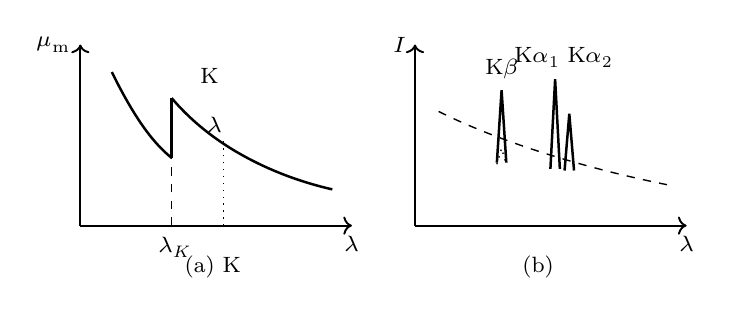
\begin{tikzpicture}[x=1cm,y=1cm]
% 左：K 吸收边的锯齿（示意）
\begin{scope}
\draw[axisline,->] (-0.10,0) -- (3.35,0) node[below,font=\fontsize{8}{9.5}\selectfont]{$\lambda$};
\draw[axisline,->] (-0.10,0) -- (-0.10,2.30) node[left,font=\fontsize{8}{9.5}\selectfont]{$\mu_{\mathrm{m}}$};
% 阀前曲线（长波侧，吸收大）
\draw[mainline] (0.30,1.95) .. controls (0.62,1.30) and (0.86,1.02) .. (1.06,0.86);
% 吸收边：向上突跃
\draw[mainline] (1.06,0.86) -- (1.06,1.62);
% 阀后曲线（短波侧，吸收小）
\draw[mainline] (1.06,1.62) .. controls (1.60,0.98) and (2.40,0.62) .. (3.10,0.46);
\draw[thinline,dashed] (1.06,0) -- (1.06,1.62);
\node[below,font=\fontsize{8}{9.5}\selectfont] at (1.10,-0.02) {$\lambda_K$};
\node[font=\fontsize{8}{9.5}\selectfont,anchor=west] at (1.30,1.90) {K 吸收边};
% 入射波长位置
\draw[thinline,dotted] (1.72,0) -- (1.72,1.10);
\node[font=\fontsize{8}{9.5}\selectfont,anchor=south] at (1.74,1.06) {$\lambda$ 入射};
\node[font=\fontsize{8}{9.5}\selectfont] at (1.75,-0.52) {(a) K 吸收边};
\end{scope}
% 右：滤波前 / 滤波后的谱（示意）
\begin{scope}[xshift=4.25cm]
\draw[axisline,->] (-0.10,0) -- (3.35,0) node[below,font=\fontsize{8}{9.5}\selectfont]{$\lambda$};
\draw[axisline,->] (-0.10,0) -- (-0.10,2.30) node[left,font=\fontsize{8}{9.5}\selectfont]{$I$};
% 连续谱包络
\draw[thinline,dashed] (0.20,1.45) .. controls (1.00,1.05) and (2.10,0.72) .. (3.10,0.52);
% K_beta 峰（未滤）
\draw[mainline] (0.94,0.80) -- (1.00,1.72) -- (1.06,0.80);
% K_alpha 双线
\draw[mainline] (1.62,0.72) -- (1.68,1.86) -- (1.74,0.72);
\draw[mainline] (1.80,0.70) -- (1.86,1.42) -- (1.92,0.70);
% 滤波后残留
\draw[thinline,dotted] (0.94,0.78) -- (1.00,0.98) -- (1.06,0.78);
\node[font=\fontsize{8}{9.5}\selectfont,anchor=south] at (1.00,1.74) {K$\beta$};
\node[font=\fontsize{8}{9.5}\selectfont,anchor=south] at (1.79,1.88) {K$\alpha_1$ K$\alpha_2$};
\node[font=\fontsize{8}{9.5}\selectfont] at (1.75,-0.52) {(b) 滤波片的作用};
\end{scope}
\end{tikzpicture}
\caption{（a）质量吸收系数随波长的变化与 K 吸收边：波长变短吸收总体下降，但在
$\lambda_K$ 处出现向上突跃。读者应看「突跃的位置」而非曲线高度，因为滤波片的选择完全
由这个位置决定。（b）滤波片的作用：滤波片的吸收边落在 K$\beta$ 与 K$\alpha$ 之间，
故 K$\beta$ 被强烈吸收（虚线为滤波后残留），而 K$\alpha_1$、K$\alpha_2$ 双线结构
\textbf{原样保留}。两图纵轴均为任意单位，曲线为示意形状，不代表任何具体测量
值。\schemamark\figsrc{据 S1（上册）图 4-7、图 4-8，书内 p.236—237 / PDF p.255—256 改绘。}}
\label{fig:mono}
\end{figure}

\subsection{衍射的几何原理：倒易空间与衍射方法}

\begin{principle}
衍射几何可以用两种等价语言表述。\textbf{Bragg 语言}只含一个角度参数，便于实测：
$2d\sin\theta=n\lambda$。\textbf{倒易空间语言}把「衍射是否发生」化为「倒易格点是否落在
Ewald 球面上」，便于理解衍射图的整体形状、仪器设计与极限球。倒易格子是正格子的一种
数学变换，二者一一对应；在多晶衍射中，Bragg 方程中的 $d$ 与 $\sin\theta$ 正是倒易关系。
\end{principle}

\subsubsection{倒易格子与正格子的关系}

设正格子由规定素单位的三个向量 $\boldsymbol{a},\boldsymbol{b},\boldsymbol{c}$ 描述，
定义三个新向量 $\boldsymbol{a}^{*},\boldsymbol{b}^{*},\boldsymbol{c}^{*}$ 使
\begin{equation}
\boldsymbol{a}^{*}\cdot\boldsymbol{a}=1,\quad
\boldsymbol{a}^{*}\cdot\boldsymbol{b}=0,\quad
\boldsymbol{a}^{*}\cdot\boldsymbol{c}=0,
\label{eq:recipdef}
\end{equation}
其余两式按 $\boldsymbol{a}\rightarrow\boldsymbol{b}\rightarrow\boldsymbol{c}$ 循环。
由式~\eqref{eq:recipdef} 与晶胞体积 $V=\boldsymbol{a}\cdot(\boldsymbol{b}\times
\boldsymbol{c})$ 可得显式表达式
\begin{equation}
\boldsymbol{a}^{*}=\frac{\boldsymbol{b}\times\boldsymbol{c}}{V},\qquad
\boldsymbol{b}^{*}=\frac{\boldsymbol{c}\times\boldsymbol{a}}{V},\qquad
\boldsymbol{c}^{*}=\frac{\boldsymbol{a}\times\boldsymbol{b}}{V}.
\label{eq:recipvec}
\end{equation}
量纲检查：分子是长度平方（叉积），分母是长度立方，故 $\boldsymbol{a}^{*}$ 的单位为
$\unit{\angstrom^{-1}}$，与式~\eqref{eq:recipdef} 点积后为纯数一致。式~\eqref{eq:recipvec}
的成立条件是\textbf{$\boldsymbol{a},\boldsymbol{b},\boldsymbol{c}$ 线性无关}（$V\neq0$）。

倒易格子有四条对衍射直接有用的性质：\textbf{（1）}它本身也是点阵，具有点阵的全部性质；
由原点指向任意格点的矢量 $\boldsymbol{H}=h\boldsymbol{a}^{*}+k\boldsymbol{b}^{*}
+l\boldsymbol{c}^{*}$ \textbf{垂直于}正格子中的平面族 $(h'k'l')$，其中
$h=nh'$、$k=nk'$、$l=nl'$，$n$ 为衍射级数。\textbf{（2）}倒易矢量长度与晶面间距成反比，
$|\boldsymbol{H}_{hkl}|=1/d_{hkl}$。\textbf{（3）}它是一种虚格子，来自正格子的数学变换，
但与正空间存在确定对应：素格子的倒易格子仍是素格子，体心格子的倒易格子是面心格子，
面心格子的倒易格子是体心格子，底心格子的倒易格子仍是底心格子。\textbf{（4）}由正格子可
唯一确定倒易格子的三个基矢长度与夹角，反之亦然。

各晶系可把参数代入式~\eqref{eq:recipvec} 简化，常用的结果列于表~\ref{tab:recip-simple}
\src{S1 §4.3.1，书内 p.238—239 / PDF p.257—258}。

\begin{table}[htbp]
\centering
\caption{几种晶系的正--倒格子参数对应（素格子）\src{据 S1 §4.3.1，书内 p.238—239 / PDF p.257—258 归纳。}}
\label{tab:recip-simple}
{\srcsize
\begin{tabularx}{\columnwidth}{@{}lXX@{}}
\toprule
晶系 & 倒格子基矢长度 & 倒格子夹角 \\
\midrule
简单立方 & $a^{*}=1/a$ & 均为 $90^{\circ}$ \\
简单四方 & $a^{*}=b^{*}=1/a$，$c^{*}=1/c$ & 均为 $90^{\circ}$ \\
六方与简单三方 & $a^{*}=b^{*}=1/(a\sin120^{\circ})$，$c^{*}=1/c$ & $\gamma^{*}=60^{\circ}$（其余 $90^{\circ}$） \\
简单正交 & $a^{*}=1/a$，$b^{*}=1/b$，$c^{*}=1/c$ & 均为 $90^{\circ}$ \\
简单单斜 & 以 $b$ 为唯一轴，$a^{*}=1/(a\sin\beta)$，$b^{*}=1/b$，$c^{*}=1/(c\sin\beta)$ & $\alpha^{*}=\gamma^{*}=90^{\circ}$，$\beta^{*}=180^{\circ}-\beta$ \\
\bottomrule
\end{tabularx}}
\end{table}

\emph{核对说明}：已对照原页面图像（书内 p.238—239 / PDF p.257—258）。原书
p.239 明列：简单立方 $a^{*}=1/a$，夹角均为 $90^{\circ}$；简单四方
$a^{*}=1/a$、$c^{*}=1/c$，夹角均为 $90^{\circ}$；\textbf{六方和简单三方
$a^{*}=1/(a\sin120^{\circ})$、$c^{*}=1/c$、
$\gamma^{*}=60^{\circ}$}；简单正交 $a^{*}=1/a$、$b^{*}=1/b$、
$c^{*}=1/c$，夹角均为 $90^{\circ}$；简单单斜以 $b$ 为唯一轴时
$a^{*}=1/(a\sin\beta)$、$b^{*}=1/b$、$c^{*}=1/(c\sin\beta)$、
$\alpha^{*}=\gamma^{*}=90^{\circ}$、
$\beta^{*}=180^{\circ}-\beta$。本表原把六方与简单三方的倒格子夹角印作「均为
$90^{\circ}$」，与原文的 $\gamma^{*}=60^{\circ}$ 不符，已据原文改正（按
$\cos\gamma^{*}=(\cos\alpha\cos\beta-\cos\gamma)/(\sin\alpha\sin\beta)$
代入 $\gamma=120^{\circ}$ 亦得 $\gamma^{*}=60^{\circ}$，可自洽复核）。
原书 p.239 另说明复格子的转换「稍微复杂一些……此不赘述」，本表后所附「素格子／复格子」提示框为改编本按
§4.3 后半段思路所加，非原表栏目。


\begin{keycond}
表~\ref{tab:recip-simple} 只对\textbf{素格子}成立。复格子（$I$、$F$、$C$、$R$）的倒易
格子转换更复杂，需要借助素格子与复格子之间的相互转换或几何作图实现。实际处理中更常用的
做法是\textbf{不换格子，而在结构因子里体现带心平移}，从而把「复格子的倒易格子」化为
「素格子的倒易格子 $+$ 系统消光条件」——这正是 4.3 节后半段的思路。
\end{keycond}

\subsubsection{倒易点阵的应用：Ewald 球、极限球与多晶德拜环}

\begin{principle}
\textbf{衍射条件。}设入射线与衍射线的单位矢量分别为 $\boldsymbol{s}_0$ 与
$\boldsymbol{s}$。晶体在倒易格点 $\boldsymbol{H}_{hkl}$ 处产生衍射的条件是
\begin{equation}
\frac{\boldsymbol{s}-\boldsymbol{s}_0}{\lambda}=\boldsymbol{H}_{hkl}
=h\boldsymbol{a}^{*}+k\boldsymbol{b}^{*}+l\boldsymbol{c}^{*}.
\label{eq:laue-vec}
\end{equation}
式~\eqref{eq:laue-vec} 左、右两侧的单位均为 $\unit{\angstrom^{-1}}$。把正空间三个基矢
分别与式~\eqref{eq:laue-vec} 点乘，用式~\eqref{eq:recipdef} 即得
\textbf{Laue 方程}
\begin{equation}
\boldsymbol{a}\cdot\Delta\boldsymbol{s}=h\lambda,\qquad
\boldsymbol{b}\cdot\Delta\boldsymbol{s}=k\lambda,\qquad
\boldsymbol{c}\cdot\Delta\boldsymbol{s}=l\lambda .
\label{eq:laue}
\end{equation}
其中 $\Delta\boldsymbol{s}\equiv\boldsymbol{s}-\boldsymbol{s}_0$ 为衍射前后单位矢
之差。Laue 方程与 Bragg 方程\textbf{完全等价}，但它涉及三个方程与更多参数；只含一个
角度参数的 Bragg 方程在实测中更常用。\src{S1 §4.3.2，书内 p.239—241 / PDF p.258—260}
\end{principle}

\begin{equation}
2d_{hkl}\sin\theta=n\lambda \qquad (n=1,2,3,\dots)
\label{eq:bragg-ch04}
\end{equation}
\begin{keycond}
\textbf{Bragg 方程的成立条件}：（1）\textbf{弹性相干散射}——散射前后波长不变，散射体
之间有确定的相位关系（这正是「晶体」而非「非晶」的前提）；（2）\textbf{入射与衍射束
共面并对称分布在晶面法线两侧}，$\theta$ 是掠射角而非入射束与法线的夹角；
（3）$d_{hkl}$ 是\textbf{互质指数} $(hkl)$ 的面间距，级数 $n$ 单独列出；若把 $n$ 并入
指数（写成 $nh\;nk\;nl$），则须取 $n=1$ 并使用对应的 $d_{nh,nk,nl}=d_{hkl}/n$，两种
写法不可混用（见式~\eqref{eq:cubic-d} 的说明）。量纲检查：$d$ 与 $\lambda$ 同为长度，
$\sin\theta$ 为纯数，量纲自洽。
\end{keycond}

对立方晶系，晶面间距与晶胞参数的关系为
\begin{equation}
\frac{1}{d_{hkl}^{2}}=\frac{h^{2}+k^{2}+l^{2}}{a^{2}}
\quad\Longrightarrow\quad
d_{hkl}=\frac{a}{\sqrt{h^{2}+k^{2}+l^{2}}}.
\label{eq:cubic-d}
\end{equation}
式~\eqref{eq:cubic-d} 的成立条件是晶胞为\textbf{立方}（$a=b=c$，$\alpha=\beta=
\gamma=90^{\circ}$）。把式~\eqref{eq:cubic-d} 代入式~\eqref{eq:bragg-ch04} 得到最常用的工作
公式
\begin{equation}
\sin^{2}\theta=\frac{\lambda^{2}}{4a^{2}}\,(h^{2}+k^{2}+l^{2}).
\label{eq:cubic-sin2}
\end{equation}
式~\eqref{eq:cubic-sin2} 是立方晶系指标化与晶胞参数精修的出发点：$\sin^{2}\theta$ 与
$(h^{2}+k^{2}+l^{2})$ 成正比，比例系数含 $a$。
式~\eqref{eq:cubic-d} 已逐字核对：原书 §4.4.1（书内 p.244 / PDF p.263）对立方、四方、
正交、六方四个晶系并列印出 $1/d^{2}$ 形式，立方系即
$\frac{1}{d^{2}}=\frac{h^{2}+k^{2}+l^{2}}{a^{2}}$；§4.6.1（书内 p.265 / PDF p.284）再次
印出该式，并令 $Q_{hkl}\equiv1/d_{hkl}^{2}$、以
$Q_{i}/Q_{j}=(h_{i}^{2}+k_{i}^{2}+l_{i}^{2})/(h_{j}^{2}+k_{j}^{2}+l_{j}^{2})$ 的比值关系做
指标化。式~\eqref{eq:cubic-sin2} 原书未直接印出，它由式~\eqref{eq:cubic-d} 代入 Bragg
方程即得（本轮写法）；原书指标化走的是 $Q$ 值比例这条路线。两式均按原书约定把衍射级数
$n$ 并入指数（原书 §4.1 已声明衍射指标 $(nh\,nk\,nl)$ 中的 $n$ 为衍射级数，晶面指数本身
互质）。\src{S1 §4.4.1 与 §4.6.1，书内 p.244、p.265 / PDF p.263、p.284}

\textbf{Ewald 反射球}（图~\ref{fig:bragg-ewald}a、b）。以晶体所在点 $A$ 为球心、
$1/\lambda$ 为半径作球。$O$ 为倒易格子原点，$\overrightarrow{AO}$ 即入射方向
$\boldsymbol{s}_0/\lambda$。若倒易格点 $B$ 落在球面上，则
$\overrightarrow{AB}=\boldsymbol{s}/\lambda$ 给出衍射方向，而
$\overrightarrow{OB}=\boldsymbol{s}/\lambda-\boldsymbol{s}_0/\lambda
=\boldsymbol{H}_{hkl}$。由图中的几何关系
\begin{equation}
OB=2\!\left(\frac{1}{\lambda}\right)\sin\theta
\quad\Longleftrightarrow\quad
OB=\frac{1}{d_{hkl}}=\left|\boldsymbol{H}_{hkl}\right| .
\label{eq:ewald-geom}
\end{equation}
式中左端由三角形的几何关系得出，中间的等价关系则由
$2d_{hkl}\sin\theta=n\lambda$ 直接给出。结论是：\textbf{倒易格子中凡落在反射球面上的点都产生衍射，衍射方向就是球心与该格点的
连线方向}。

\textbf{多晶为什么给出环，粉末衍射仪上又为什么变成峰。}对单晶，给定波长时必须不断改变
晶体取向才能让倒易格子与反射球相交。对多晶样品，\textbf{大量微晶无规取向}，同一个
$(hkl)$ 的倒易点在空间中绕原点扫出一个半径 $1/d_{hkl}$ 的\textbf{球面}；该倒易球面与
Ewald 反射球（半径 $1/\lambda$，球心在 $A$）相交成一个\textbf{圆}。衍射方向沿
$\overrightarrow{AB}$ 扫出以入射方向为轴、半顶角 $2\theta$ 的圆锥面——在平板探测器或
德拜相机上就是一条\textbf{德拜环}。粉末衍射仪中，探测器只在与入射束共面、且满足
$FS=SD$ 的聚焦几何方向上接收（见 4.3.3），只切到这个圆锥的一条母线，于是环被「读成」
一个\textbf{峰}，横轴为 $2\theta$。这就是「同一份数据，照相法看到环、衍射仪看到峰」的
原因。

\textbf{极限球。}只有落在以 $O$ 为中心、半径 $R=2/\lambda$ 的球内的倒易格点才可能产生
衍射，该球称\textbf{衍射极限球}。由 $\sin\theta\le1$ 及
$|\boldsymbol{H}|=2\sin\theta/\lambda$ 可得 $|\boldsymbol{H}|\le2/\lambda$，换言之
\textbf{只有 $d\ge\lambda/2$ 的衍射是可达的}。由此：X 射线波长越短，可收集的衍射范围
越大、衍射线越密；倒易格子越密，收集到的衍射越多。所以\textbf{波长选择要按样品定}——
晶面间距 $d$ 大的样品宜用长波长 X 射线，否则大量低角信息落在极限球之外；而多晶衍射
反而常用较长的 Cu 靶（$\lambda=\qty{1.54}{\angstrom}$）以\textbf{尽量拉开衍射角、
减少峰重叠}，单晶衍射则常用 Mo 靶（$\lambda\approx\qty{0.71}{\angstrom}$）以多收
数据点。两者的取舍方向恰好相反。\src{S1 §4.3.2，书内 p.240—241 / PDF p.259—260}

\begin{figure}[htbp]
\centering
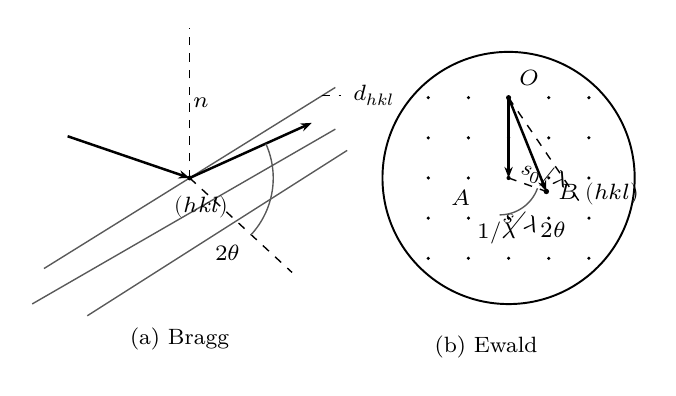
\begin{tikzpicture}[x=1cm,y=1cm]
% (a) Bragg 构型
\begin{scope}
\coordinate (O) at (0,0);
\coordinate (nO) at (0,1.90);
\coordinate (Apt) at (-1.55,0.53);
% 晶面族
\draw[accent,thinline] (-1.85,-1.15) -- (1.85,1.15);
\draw[accent,thinline] (-2.00,-1.60) -- (1.85,0.62);
\draw[accent,thinline] (-1.30,-1.75) -- (2.00,0.35);
\fill (O) circle (0.9pt);
\node[font=\fontsize{8}{9.5}\selectfont,anchor=north] at (0.02,-0.10) {晶面 $(hkl)$};
% 法线
\draw[thinline,dashed] (O) -- (nO);
\path (O) -- (nO) node[font=\fontsize{8}{9.5}\selectfont,midway,anchor=west,inner sep=1pt] {$n$};
% 入射线与延长线
\draw[mainline,-{Stealth[length=4pt]}] (Apt) -- (O);
\draw[thinline,dashed] (O) -- (1.30,-1.20);
\node[font=\fontsize{8}{9.5}\selectfont,anchor=east] at (-1.58,0.56) {入射线};
% 衍射线
\draw[mainline,-{Stealth[length=4pt]}] (O) -- (1.55,0.70);
\node[font=\fontsize{8}{9.5}\selectfont,anchor=west] at (1.58,0.72) {衍射线};
% 2theta 弧
\draw[thinline,accent] (0.78,-0.72) arc[start angle=-42.7,end angle=24.3,radius=1.06];
\node[font=\fontsize{8}{9.5}\selectfont] at (0.48,-0.95) {$2\theta$};
% 面间距 d 与间距标记
\draw[thinline,dashed] (1.68,1.05) -- (1.92,1.05);
\node[font=\fontsize{8}{9.5}\selectfont,anchor=west] at (1.95,1.05) {$d_{hkl}$};
\node[font=\fontsize{8}{9.5}\selectfont] at (0,-2.05) {(a) Bragg 构型};
\end{scope}
% (b) Ewald 球
\begin{scope}[xshift=4.05cm,scale=1.02]
\coordinate (A) at (0,1);
\coordinate (C) at (0,0);
\draw[axisline] (C) circle (1.57);
% 倒易格子点
\foreach \xx in {0,0.5,1.0,1.5,-0.5,-1.0,-1.5}{
  \foreach \yy in {1.0,0.5,0,-0.5,-1.0}{
    \pgfmathsetmacro{\rr}{sqrt(\xx*\xx+\yy*\yy)}
    \pgfmathparse{(\rr>0.18)&&(\rr<1.50)?1:0}
    \ifnum\pgfmathresult=1
      \fill[black] (\xx,\yy) circle (0.022);
    \fi
  }
}
\fill (A) circle (0.032);
\node[font=\fontsize{8}{9.5}\selectfont,anchor=south west] at (0.02,1.02) {$O$（倒易原点）};
\fill (C) circle (0.026);
\node[font=\fontsize{8}{9.5}\selectfont,anchor=north east] at (-0.04,-0.02) {$A$（晶体）};
% 入射 / 衍射方向
\draw[mainline,-{Stealth[length=4pt]}] (A) -- (C);
\draw[mainline,-{Stealth[length=4pt]}] (A) -- (0.47,-0.168);
\draw[thinline,dashed] (A) -- (0.9,-0.322);
\draw[thinline,dashed] (C) -- (0.47,-0.168);
\fill (0.47,-0.168) circle (0.034);
\node[font=\fontsize{8}{9.5}\selectfont,anchor=west] at (0.50,-0.20) {$B$ $(hkl)$};
\node[font=\fontsize{8}{9.5}\selectfont,anchor=west,rotate=-19] at (0.06,0.16) {$\boldsymbol{s}_0/\lambda$};
\node[font=\fontsize{8}{9.5}\selectfont,anchor=north,rotate=-19] at (0.24,-0.30) {$\boldsymbol{s}/\lambda$};
\node[font=\fontsize{8}{9.5}\selectfont,anchor=north] at (-0.14,-0.42) {$1/\lambda$};
\draw[thinline,accent] (0.36,-0.128) arc[start angle=-19.7,end angle=-90,radius=0.50];
% 【重叠修正，2026-09-30】$2\theta$ 原在 (0.16,-0.60)，与 rotate=-19 的
% $\boldsymbol{s}/\lambda$ 标注尾巴相碰：实测 $\lambda$ 墨迹 [363.3,368.7]×[481.9,488.3]
% 与 $2$ 墨迹 [366.2,370.1]×[484.0,489.3] 相交 2.5×4.3 pt，轮廓交叠 0.417 pt²。
% 右移 0.12 cm、下移 0.04 cm 至 (0.28,-0.64)。
\node[font=\fontsize{8}{9.5}\selectfont,anchor=west] at (0.28,-0.64) {$2\theta$};
\node[font=\fontsize{8}{9.5}\selectfont,anchor=north] at (0,-1.85) {(b) Ewald 球与倒易格点};
\end{scope}
\end{tikzpicture}
\caption{\sloppy 衍射几何的两种等价表述。\textbf{（a）Bragg 构型}：读者应看三件事——$\theta$ 是
入射束与晶面之间的掠射角，晶面法线与入射线和衍射线夹角的平分线重合，衍射束与入射束的
夹角为 $2\theta$；同一族晶面中只有满足 $2d\sin\theta=n\lambda$ 的角度才出射，这就是
「峰位只由 $d$ 与 $\lambda$ 决定」的几何来源。\textbf{（b）Ewald 球}：球心 $A$ 是晶体，
球半径为 $1/\lambda$，倒易原点 $O$ 落在球面上。凡落在球面上的倒易格点（如 $B$）都
产生衍射：由球心指向该格点的方向即衍射方向，格点矢量 $H_{hkl}$ 的长度等于 $1/d_{hkl}$。
多晶样品中各微晶的同一 $(hkl)$ 倒易点绕 $O$ 扫成球面，该球面与 Ewald 球相交成圆，
衍射方向随之扫成圆锥，在探测器或底片上即为德拜环。两图均为矢量关系的示意，格点间距
与球半径的比例不代表任何具体晶体。\schemamark\figsrc{据 S1（上册）图 4-9，书内 p.240 /
PDF p.259 改绘（本图另补入 Bragg 构型以便对照）。}}
\label{fig:bragg-ewald}
\end{figure}

\subsubsection{峰位、峰强与峰形各自携带什么信息}

把上面的几何换成三个可读量（图~\ref{fig:pattern-info}），本章后面的所有方法都是这三条线
的延伸。

\begin{equation}
F(hkl)=\sum_{j=1}^{N} f_j\,
\exp\!\left[\,2\pi i\,(hx_j+ky_j+lz_j)\,\right]
=\sum_{j=1}^{N} f_j\,\mathrm{e}^{\mathrm{i}\varphi_j},
\label{eq:sf}
\end{equation}
\begin{equation}
\varphi_j=2\pi\,(hx_j+ky_j+lz_j),
\label{eq:phase}
\end{equation}
% 【重叠修正，2026-09-30】原来写的是 $L\!P$：`\!` 是**负** 3mu 细空（10 pt 下 −1.67 pt），
% 把斜体 L 的脚压进斜体 P 的竖干里。实测 p.66 两处、p.67 一处轮廓真实交叠
% 0.96 / 0.96 / 0.61 pt²（墨迹盒重叠 1.7×6.5、1.3×5.2 pt）。
% 去掉 `\!` 后两字母各按自身边距相接，不再相交。LP 是缩写，本不需要收紧。
\begin{equation}
I(hkl)\propto\left|F(hkl)\right|^{2}\cdot LP\cdot D\cdot\Delta V\cdot j,
\label{eq:intensity}
\end{equation}
式~\eqref{eq:sf} 中 $f_j$ 是第 $j$ 个原子的\textbf{原子散射因子}，$(x_j,y_j,z_j)$ 是其
分数坐标，$N$ 为晶胞内原子数，$\varphi_j$ 为该原子的相位；$|F(hkl)|^{2}$ 决定该衍射的
\textbf{本征强度}。
式~\eqref{eq:intensity} 中 $LP$ 为 Lorentz--偏振因子，$D$ 为温度因子，$\Delta V$ 为参与
衍射的样品体积，$j$ 为多重度因子。量纲检查：$f_j$ 以「一个电子的散射振幅」为单位，
$\varphi_j$ 为纯数（$h,k,l$ 与分数坐标均无量纲），故 $F$ 与 $I$ 均为相对量，实际工作中
以相对强度报告。
两式已逐字核对：原书 §4.4.3（书内 p.249—250 / PDF p.268—269）先给二原子式
$F_{hkl}=f_A+f_B\exp[\mathrm{i}2\pi(hx+ky+lz)]$，再给一般式
$F_{hkl}=\sum_{i}^{n}f_i\exp[2\pi\mathrm{i}(hx_i+ky_i+lz_i)]$，相位式亦作
$\varphi=(\Delta/\lambda)\times2\pi=2\pi(hx+ky+lz)$，与式~\eqref{eq:sf}、
\eqref{eq:phase} 一致。强度式按原书 §4.4.2（书内 p.245—246 / PDF p.264—265）校正为
$I_{hkl}=K'PL|F_{hkl}|^{2}D\Delta Vj$：原书把 $P$ 与 $L$ 分写
（$P=(1+\cos^{2}2\theta)/2$，$L=1/(2\sin^{2}\theta\cos\theta)$，合称 $PL$ 因子），温度因子
写作 $D=\exp(-B\sin^{2}\theta/\lambda^{2})$（$B=8\pi^{2}U$，$U=\langle u^{2}\rangle$），
\textbf{不设独立的吸收因子 $A(\theta)$}——吸收并入体积因子 $\Delta V$（平行板样品
$\Delta V=A_0/2\mu$，与 $\theta$ 无关）。本节原写的 $A(\theta)\cdot\exp(-2M)$ 已按原书订正。
\src{S1 §4.4.2、§4.4.3，书内 p.245—246、p.249—250 / PDF p.264—265、p.268—269}

\begin{keycond}
\textbf{结构因子与系统消光的关键条件}：（1）式~\eqref{eq:sf} 求和\textbf{只对晶胞内
全部原子}进行，原子种类由 $f_j$ 体现，位置由相位 $\varphi_j$ 体现；因此
\textbf{「点阵型式」不足以决定消光规律，必须连基元一起算}。（2）\textbf{消光只发生在
$F(hkl)\equiv0$ 时}，其后果是\textbf{系统性缺失}（整族反射全无），而不是强度偏低；
强度偏低的反射可能只是弱，不能据此判断消光。（3）温度因子使 $f_j$ 随 $\sin\theta/\lambda$
增大而衰减，即\textbf{高角峰系统性偏弱}，这是比较峰强时必须先做的归一化。
\end{keycond}

\begin{table}[htbp]
\centering
\caption{常见点阵与基元的系统消光条件（$n$ 为整数）\src{本表为本改编本归纳，非源书表格；依据 S1 §4.1.2，书内 p.227—231 / PDF p.246—250；§4.3，书内 p.239—241 / PDF p.258—260。表中消光条件由结构因子 $F(hkl)=0$ 推出，非源书实验数据。}}
\label{tab:extinction-ch04}
{\srcsize
\begin{tabularx}{\columnwidth}{@{}lXX@{}}
\toprule
类型 & 出现的反射 & 系统缺失的反射 \\
\midrule
简单立方（$cP$） & 全部 $hkl$ & 无 \\
体心立方（$cI$） & $h+k+l$ 为偶数 & $h+k+l$ 为奇数 \\
面心立方（$cF$） & $h,k,l$ 全奇或全偶 & $h,k,l$ 奇偶混杂 \\
金刚石型（$cF$ $+$ 双原子基元） & $h,k,l$ 全奇，或全偶且 $h+k+l=4n$ & 全偶但 $h+k+l\neq4n$（如 200、222） \\
NaCl 型（$cF$ $+$ 双原子基元） & $h,k,l$ 全奇或全偶 & $h,k,l$ 奇偶混杂 \\
\bottomrule
\end{tabularx}}
\end{table}

\begin{pitfall}
表~\ref{tab:extinction-ch04} 第 3 行与第 4、5 行是同一 $cF$ 点阵下的不同基元，消光规律却
不同：\textbf{把「$cF$ 就一定全奇全偶」当成本质规律，会误判金刚石型与 NaCl 型结构}。
同理，$cI$ 点阵的 $h+k+l$ 奇数缺失只说明「点阵带心」，要确定空间群还必须把滑移面
（$a$、$b$、$c$、$n$、$d$、$e$）与螺旋轴引起的\textbf{条件消光}一并列出——只知道「有
系统缺失」不等于知道「哪个空间群」。\src{S1 §4.1.2、§4.3，书内 p.227—231、p.239—241 /
PDF p.246—250、p.258—260}
\end{pitfall}

\begin{dataflow}
三个可读量到结论的对应关系是本章的骨架：
\textbf{峰位（$2\theta$）}$\rightarrow$ Bragg 方程 $\rightarrow$ $d$ 值 $\rightarrow$
指标化 $\rightarrow$ 晶胞参数与物相；\textbf{峰强} $\rightarrow$ 结构因子与占据/含量
$\rightarrow$ 原子位置、相对含量（定量）；\textbf{峰形（半高宽、线型）}$\rightarrow$
晶粒尺寸（Scherrer）、微应变、堆垛层错，但要\textbf{先扣除仪器宽化}。三条线索互相独立
又互相依赖：峰位错了，指标化就错，$|F|^{2}$ 的比较也就失去意义。
\end{dataflow}

\begin{figure}[htbp]
\centering
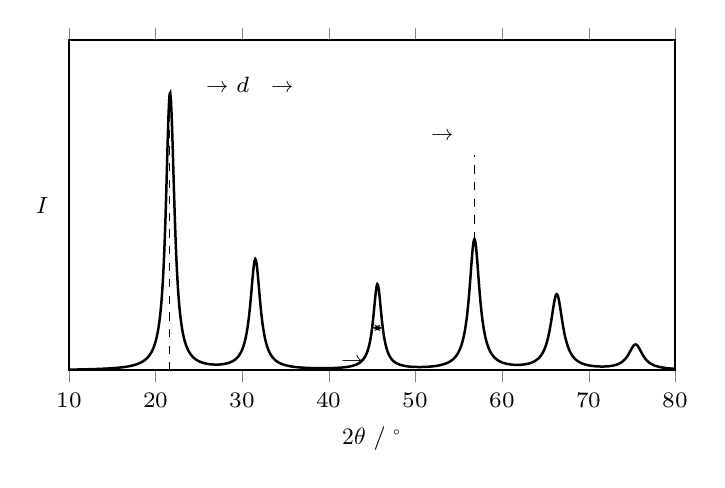
\begin{tikzpicture}
\begin{axis}[
  width=77mm, height=42mm,
  scale only axis,
  xmin=10, xmax=80, ymin=0, ymax=1.32,
  xlabel={$2\theta$ / $^{\circ}$}, ylabel={$I$}, ylabel style={rotate=-90},
  xtick={10,20,30,40,50,60,70,80},
  ytick=\empty,
  axis line style={axisline},
]
\addplot[domain=10:80,samples=900,mainline,black]
  {0.90/(1+((x-21.6)/0.55)^2)
  +0.26/(1+((x-21.9)/0.55)^2)
  +0.44/(1+((x-31.5)/0.70)^2)
  +0.34/(1+((x-45.6)/0.60)^2)
  +0.52/(1+((x-56.8)/0.72)^2)
  +0.30/(1+((x-66.3)/0.85)^2)
  +0.10/(1+((x-75.4)/1.0)^2)};
% 峰位标注
\draw[thinline,dashed] (21.6,0) -- (21.6,1.02);
\node[font=\fontsize{8}{9.5}\selectfont,anchor=west,align=left] at (22.4,1.14)
  {峰位 $\rightarrow$ $d$ 值 $\rightarrow$ 晶胞参数、物相};
% 峰强标注
\draw[thinline,dashed] (56.8,0.52) -- (56.8,0.86);
\node[font=\fontsize{8}{9.5}\selectfont,anchor=west,align=left] at (48.4,0.94)
  {峰强 $\rightarrow$ 结构因子、含量};
% 峰宽标注
\draw[thinline,{Stealth[length=3pt]}-{Stealth[length=3pt]}] (45.0,0.17) -- (46.2,0.17);
\node[font=\fontsize{8}{9.5}\selectfont,anchor=north west,align=left] at (38.0,0.10)
  {峰宽 $\rightarrow$ 晶粒尺寸、微应变（须扣仪器宽化）};
\end{axis}
\end{tikzpicture}
\caption{峰位、峰强、峰形三种信息的读法。读者应看三处标注分别指向横轴位置、纵轴高度与
峰的半高宽：峰位是三者中\textbf{唯一可以做到高精度}的量，因为 $d$ 的相对误差与
$\cot\theta$ 乘测角误差同量级，高角峰位因此更准；峰强受结构因子、择优取向、吸收与
温度因子多重影响，定量前必须校正；峰宽则是尺寸、应变与仪器宽化的\textbf{卷积}，三者
不能凭一条峰分开。纵轴 $I$ 为相对强度，本图为按有界线型函数（Lorentz 型）计算的模型图，
峰位与峰强由教学设定，不代表任何真实样品。\modelmark\pedset{峰位与相对强度为教学设定
值。}}
\label{fig:pattern-info}
\end{figure}

\begin{crosscheck}
XRD 的能力边界集中在表~\ref{tab:xrd-limits}：它给的是\textbf{长程有序的平均结构}，
对局部结构、非晶、轻元素和纳米尺度信息要么不敏感、要么只能给「等效值」。凡是要下这类
结论，都应当找互补手段回查，而不是把一条衍射曲线解释到极限。
\end{crosscheck}

\begin{table}[htbp]
\centering
\caption{XRD 能给出什么／不能给出什么\src{据 S1 §4.1—§4.3，书内 p.219—243 / PDF p.238—262 归纳。}}
\label{tab:xrd-limits}
{\srcsize
\begin{tabularx}{\columnwidth}{@{}lXX@{}}
\toprule
维度 & 能可靠给出 & 不能给出或只能给等效值 \\
\midrule
有序性 & 长程有序：晶胞参数、点阵型式、空间群线索 & 短程有序、局部配位、非晶结构（非晶无峰，只出弥散包） \\
原子位置 & 重原子位置与占位（配合精修） & 氢与轻元素位置（$f$ 太小，几乎不贡献强度） \\
物相 & 晶态物相鉴定与相对含量（需校正） & 非晶相含量、无定形表面层、单层分散物种的归属 \\
尺寸与应变 & 相干衍射域尺寸（Scherrer，纳米级）与微应变的\textbf{耦合}结果 & 两者分开需要线型分析或多峰拟合；峰宽同时含仪器宽化 \\
峰位误差 & 高角峰位精度可达 $10^{-4}$ 量级（$2\theta$） & 样品高度偏差、透明度、轴向发散引起的系统偏差不能靠平均消除 \\
\bottomrule
\end{tabularx}}
\end{table}

\emph{核对说明}：本轮重核（PDF p.240—241 = 书内 p.221—222 页面图像逐字对读）：
「能可靠给出」一栏五行的原文依据逐句核对无误；§4.1 的其余页（书内 p.220、p.223—225、
p.227—232）不作为本表任何一行的依据，「不能给出」一栏整栏为改编归纳，故上述各页不构成证据缺口。
逐行核对：「能可靠给出」一栏的主体有据于 p.221—222 的逐字表述——原书先写「在多晶 X 射线衍射图上，
可以直接读出的信息是：衍射峰的位置、衍射峰的强度和衍射峰的形状」，随后写「衍射峰的系统缺失（即系统消光）
给出晶体点阵类型和空间群的信息，峰位置在何处由晶胞参数决定；衍射峰强度反映了晶胞中原子位置和分布的状况；
而衍射峰的形状与仪器几何光路及条件、晶粒大小、晶格畸变等密切相关」，并记「利用多晶衍射数据，
可以得到样品的物相组成与含量、晶体的点阵参数、晶粒大小等信息」。据此，第 1 行（点阵型式与空间群线索）、第 2
行（晶胞中的原子位置）、第 3 行（物相组成与含量）、第 4 行（晶粒大小与晶格畸变的耦合、峰宽含仪器几何条件）
均有原文对应；p.222 并记多晶衍射可用于 Rietveld 精修乃至晶体结构的从头确定。
改编补充：「不能给出或只能给等效值」一栏系改编本据 XRD 的固有限制归纳，本次所读 §4.1
各页未出现非晶只出弥散包、氢与轻元素的散射因子过小、非晶相含量、无定形表面层、单层分散物种等表述；第 2
行的「重原子」「配合精修」、第 3 行的「需校正」、第 4 行的「相干衍射域」「Scherrer」
命名与「分开需要线型分析或多峰拟合」的判据，同属归纳。第 5 行（峰位误差）整行亦为改编补充：高角峰位精度
$10^{-4}$ 量级、以及样品高度偏差、透明度、轴向发散引起的系统偏差，本次所读 §4.1 各页未涉及；本分片
「误判与边界」处已另行记明原书对样品位移引起的 $\Delta(2\theta)$ 的表达式载于 §4.7（分片
c 范围），而本分片 §4.2—§4.3（书内 p.234—243 / PDF p.253—262）
在早前批次已核对，原书该段未给出「偏移量随 $\cos\theta$ 变化」的量化式。


\begin{pitfall}
\textbf{峰位系统误差必须与随机误差分开处理。}（1）\textbf{样品高度偏差}：样品表面偏离
测角仪聚焦圆时，峰位整体偏移，且偏移量随 $2\theta$ 变化——低角与高角偏移方向相反、
在 $2\theta=180^{\circ}$ 附近趋近于零。因此\textbf{用「内标」或「高角反射外推」可以
校正，用「多点平均」不能}。（2）\textbf{样品透明度的深度穿透}：轻元素样品的 X 射线
穿透深度大，衍射「重心」位于样品表面之下，等效于高度偏差。（3）\textbf{K$\alpha_2$
未剥离}：在低角区 K$\alpha_1$ 与 K$\alpha_2$ 重叠成不对称峰，此时若用峰顶读
$2\theta$，得到的是混合波长对应的位置，报告的 $d$ 值会随分峰方式而变。
样品高度偏差的量化关系（偏移量 $\propto\cos\theta$、在 $2\theta=180^{\circ}$ 处为零、
低角与高角偏移方向相反）系按聚焦几何的标准结论写出的表述：已核原书分片 a 的范围
（§4.2—§4.3，书内 p.234—243 / PDF p.253—262），原书该段止于聚焦法的优缺点与衍射仪
$\theta$--$2\theta$ 联动扫描几何（书内 p.243 / PDF p.262），\textbf{未给出}此量化式，
故此处为改编补充。原书对样品位移引起的 $\Delta(2\theta)$ 另有表达式，载于 §4.7（分片 c
的范围），其形式与取值见分片 c 对应处。
\end{pitfall}

\begin{measure}
\textbf{实际测量中必须记录的实验条件}（缺一项，后续结论就无法回查）：
靶材与滤光/单色方式（Cu K$\alpha$ 是否已剥离 K$\alpha_2$、有无 Ni 滤片或石墨单色器）、
管压与管流、发散狭缝与接收狭缝、扫描步长与每步计数时间、$2\theta$ 扫描范围、
样品制备方式（压片还是涂片、是否加内标、是否转动以抑制择优取向）。
\textbf{判据}：若同一个样品两次测量的峰位差超过 $0.05^{\circ}$（$2\theta$），应先查
制样与高度，再谈物相与晶胞参数的差异。\src{S1 §4.2—§4.3，书内 p.234—243 /
PDF p.253—262}
\end{measure}

\begin{methodsum}
分片 a 建立的链条是：\textbf{周期性}决定「有衍射」，\textbf{对称性与基元}决定「哪些
衍射系统缺失」，\textbf{Ewald 球几何}决定「衍射出现在哪个 $2\theta$」（多晶中经德拜环
退化为峰），\textbf{结构因子}决定「峰有多强」，\textbf{仪器与制样}决定「峰位准不准、
峰形被污染多少」。三张表（晶系与布拉维格子、常见消光条件、XRD 能力边界）与三个公式
（Bragg、结构因子、倒易--Ewald 关系）是后续分片反复调用的公共接口。
\end{methodsum}

\srcnote{本节依据 S1（上册）第 4 章 4.1—4.3 节编写，覆盖书内 p.219—243 /
PDF p.238—262。原书 4.1.2 中宏观对称要素表（表 4-1）、螺旋轴与滑移面表（表 4-3、
表 4-4）、空间群国际记号三个位方向（表 4-5）与 $P2_1/c$ 等效点系（表 4-6）属群论
细节，本分片按压缩原则未逐表转录，只保留与衍射判读直接相关的结论；需要查阅原子坐标
生成规则时请回原文。}
}{}
\IfFileExists{chapters/parts/ch04-b.tex}{\subsection{晶体对 X 射线的衍射}
\src{上册 §4.4，书内 p.244—253 / PDF p.263—272}

多晶衍射实验最终只给出两列数：每个峰的衍射角 $2\theta$ 与它的强度 $I$。本节余下内容的全部
推论都建立在一个分工上——\textbf{峰位}只由晶胞的平移周期决定，因而给出晶面间距与点阵参数；
\textbf{峰强}由晶胞内原子的种类、坐标、占位与热振动决定；\textbf{峰的有无}（系统消光）由点阵
类型与微观对称元素决定。三条线索彼此独立又互相印证，是物相鉴定、相定量、指标化乃至结构精修
的公共基础。

\begin{probout}
\textbf{测什么}：一套 $(2\theta,\,I)$ 峰表，以及由此换算的晶面间距 $d$ 与相对强度 $I/I_1$。\\
\textbf{能推断什么}：$d$ 序列 $\rightarrow$ 晶胞参数与点阵类型（配合系统消光）；强度分布
$\rightarrow$ 晶胞内原子的位置、种类、占位度与热振动；整套图谱 $\rightarrow$ 物相种类，多相样品
中各相相对含量。\\
\textbf{不能推断什么}：衍射实验中相位信息丢失，实测只给出 $|F_{hkl}|$，因此粉末强度本身不足以
唯一确定原子坐标；轻原子（$Z$ 小）与低含量相（$\lesssim 3\%$）在强度上贡献很小，属于方法本身的
边界而非操作失误。
\end{probout}

\subsubsection{衍射峰的位置与晶面间距}

\begin{principle}
衍射出现的必要条件（布拉格方程）
\begin{equation}
2\,d_{hkl}\sin\theta=\lambda ,
\label{eq:ch04b-bragg}
\end{equation}
它把可观测量 $\theta$ 与结构量 $d_{hkl}$ 联系起来。晶面间距由晶格常数 $a,b,c$ 及三个夹角
$\alpha,\beta,\gamma$（或其倒易点阵常数 $a^{*},b^{*},c^{*}$ 与 $\alpha^{*},\beta^{*},\gamma^{*}$）
和衍射指标 $h,k,l$ 共同决定。以倒易格子向量 $\vec{H}=h\vec{a}^{*}+k\vec{b}^{*}+l\vec{c}^{*}$
为工具，可得
 
\begin{equation}
Q\equiv\frac{1}{d_{hkl}^{2}}=\left|\vec{H}\right|^{2},
\label{eq:ch04b-Q}
\end{equation}
即 $Q$ 是倒易向量长度的平方。$Q$ 的引入使“峰位 $\rightarrow$ 结构”的关系在一个晶系内变成线性
关系：立方、四方、六方、正交晶系中 $Q$ 都是 $h,k,l$ 平方项之和。此处已对照原页面图像
（书内 p.244—245 / PDF p.263—264）：原书\textbf{并未印出通式} $Q\equiv1/d^{2}=|\vec{H}|^{2}$，
而是逐晶系直接给出 $1/d^{2}$ 的表达式——p.244 给立方、四方、正交、六方四式，p.245 给单斜、
三斜两式，并另行给出 R 格子取素晶格（$a=b=c$、$\alpha=\beta=\gamma$）时的简化式
$1/d^{2}=(h^{2}+k^{2}+l^{2})a^{*2}+2(hk+kl+hl)a^{*2}\cos\alpha^{*}$。原书只说明「利用倒易格子向量
$\vec{H}=h\vec{a}^{*}+k\vec{b}^{*}+l\vec{c}^{*}$ 及其与晶面间距之间的关系，可以求出……数学关系」。
故以 $\vec{H}$ 长度平方定义 $Q$、把各晶系写成统一的 $Q$ 记号，是本书为把「峰位 $\rightarrow$ 结构」
写成线性关系而引入的组织方式，不是原书原符号；下表各式的数学内容与原书逐式等价，只是原书
单斜、三斜、菱方形用倒易点阵常数表达，本表改写为直接晶格常数的等价式。
\end{principle}

\begin{table}[tbp]
  \centering
  \caption{各晶系的 $Q=1/d^{2}$ 表达式的标准形式，以及需要确定的独立晶胞参数个数。单斜式取
    $b$ 轴唯一（$\beta$ 为 $a$ 与 $c$ 的夹角）。\src{据 S1（上册）§4.4.1，书内 p.244—245 / PDF p.263—264 归纳。}}
  \label{tab:ch04b-Qtable}
  \begin{tabular}{@{}llc@{}}
    \toprule
    晶系 & $Q=1/d^{2}$ & 独立参数 \\
    \midrule
    立方 & $\dfrac{h^{2}+k^{2}+l^{2}}{a^{2}}$ & 1 \\
    四方 & $\dfrac{h^{2}+k^{2}}{a^{2}}+\dfrac{l^{2}}{c^{2}}$ & 2 \\
    六方（三方取六方轴） & $\dfrac{4(h^{2}+hk+k^{2})}{3a^{2}}+\dfrac{l^{2}}{c^{2}}$ & 2 \\
    菱方（取菱方轴） & $\dfrac{(h^{2}+k^{2}+l^{2})\sin^{2}\alpha+2(hk+kl+lh)(\cos^{2}\alpha-\cos\alpha)}
      {a^{2}(1-3\cos^{2}\alpha+2\cos^{3}\alpha)}$ & 2 \\
    正交 & $\dfrac{h^{2}}{a^{2}}+\dfrac{k^{2}}{b^{2}}+\dfrac{l^{2}}{c^{2}}$ & 3 \\
    单斜 & $\dfrac{1}{\sin^{2}\beta}\left(\dfrac{h^{2}}{a^{2}}+\dfrac{k^{2}\sin^{2}\beta}{b^{2}}
      +\dfrac{l^{2}}{c^{2}}-\dfrac{2hl\cos\beta}{ac}\right)$ & 4 \\
    \bottomrule
  \end{tabular}
\end{table}

三斜晶系（6 个独立参数）不适合写成一个紧凑分式，通常用倒易度量张量分量的形式：
\begin{equation}
Q=\frac{1}{V^{2}}\left(S_{11}h^{2}+S_{22}k^{2}+S_{33}l^{2}+2S_{12}hk+2S_{13}hl+2S_{23}kl\right),
\label{eq:ch04b-triclinic}
\end{equation}
其中 $S_{11}=b^{2}c^{2}\sin^{2}\alpha$，$S_{22}=a^{2}c^{2}\sin^{2}\beta$，$S_{33}=a^{2}b^{2}\sin^{2}\gamma$，
$S_{12}=abc^{2}(\cos\alpha\cos\beta-\cos\gamma)$，$S_{13}=ab^{2}c(\cos\alpha\cos\gamma-\cos\beta)$，
$S_{23}=a^{2}bc(\cos\beta\cos\gamma-\cos\alpha)$，
$V=abc\sqrt{1-\cos^{2}\alpha-\cos^{2}\beta-\cos^{2}\gamma+2\cos\alpha\cos\beta\cos\gamma}$。
此处已对照原页面图像（书内 p.245 / PDF p.264）：原书三斜式印为
$1/d^{2}=h^{2}a^{*2}+k^{2}b^{*2}+l^{2}c^{*2}+2hka^{*}b^{*}\cos\gamma^{*}+2klb^{*}c^{*}\cos\alpha^{*}
+2hla^{*}c^{*}\cos\beta^{*}$，单斜式印为
$1/d^{2}=h^{2}a^{*2}+k^{2}b^{*2}+l^{2}c^{*2}+2hla^{*}c^{*}\cos\beta^{*}$，均用\textbf{倒易点阵常数}
表达。式~\equref{eq:ch04b-triclinic} 的 $S_{ij}$ 记号是本项目为可读性引入的约定（等价于倒易度量
张量分量写法），与原书符号不同但数学内容一致。

\begin{measure}
\textbf{峰位怎么读}。$2\theta$ 的取值方式直接决定 $d$ 的精度：峰顶法读数受统计涨落影响最大，
重心法和全谱拟合（剖面对峰形建模后取峰位）精度最高，弱峰尤其要用拟合而不是目测峰顶。
\textbf{必须做的三项校正}：（i）剥离 $K\alpha_{2}$（$K\alpha_{1}/K\alpha_{2}$ 双线使峰不对称，
未剥离时 $d$ 系统偏大）；（ii）校正仪器零点与样品位移（样品表面偏离测角仪圆心，$d$ 的系统误差
近似正比于 $\cos\theta$，低角度最敏感）；（iii）用内标物（如 \ce{SiO2} 石英、\ce{CaF2}、Si）
把实测 $d$ 归算到标准值上。波长取 $K\alpha_{1}$ 单线时 Cu 靶为 $1.5406$ Å，取 $K\alpha$ 加权
平均值时为 $1.5418$ Å；两者混用会引入约 $0.05\%$ 的系统偏差。
\end{measure}

\begin{dataflow}
$2\theta$（已剥离 $K\alpha_{2}$、已做位移与内标校正）$\rightarrow$ 由式~\equref{eq:ch04b-bragg} 得
$d_{hkl}$ $\rightarrow$ 由式~\equref{eq:ch04b-Q} 得 $Q$ $\rightarrow$ 对每个可能的指标 $(hkl)$
写出一个线性方程 $\rightarrow$ 最小二乘解出晶胞参数 $\rightarrow$ 高角度线权重更大（$\Delta d/d$
随 $\theta$ 增大而减小），故晶胞参数精修应优先采用高角线并作外推。
\end{dataflow}

\begin{pitfall}
把峰位误差当成结构信息的三种典型情形：\\
（1）\textbf{样品位移}造成所有峰的 $d$ 同向偏移，看起来像“晶胞整体胀大”。判别方法：加内标后
偏移是否消失；或看 $\Delta d/d$ 是否随 $\cos\theta$ 规律变化而非随机。\\
（2）\textbf{未剥离 $K\alpha_{2}$}使每个峰出现“肩”，重心法读数介于两条线之间，$d$ 偏大且偏移
随角度变化，容易被误读为固溶导致的晶胞参数变化。\\
（3）\textbf{峰位随温度漂移}（热膨胀）。同一批样品在不同温度或不同时间测量时，$d$ 的小幅变化
要先排除温度因素，再讨论成分或缺陷。
\end{pitfall}

\begin{crosscheck}
峰位得到的晶胞参数必须与指标化结果（见 §4.6）互校：若一套指标能给出一致的晶胞参数且能指标化
全部衍射线，则峰位数据自洽；若不能，往往是指标化选错或存在未识别的第二相。进一步可与 PDF
卡片值、单晶结构数据、以及化学分析给出的元素比互校。
\end{crosscheck}

\subsubsection{多晶衍射峰的强度}

\begin{principle}
多晶（粉末）样品的衍射强度是“单晶某一 $hkl$ 的散射能力”乘上一系列几何与物理修正后的结果。
本书采用的简化形式为
\begin{equation}
I_{hkl}=K\cdot\left|F_{hkl}\right|^{2}\cdot P\cdot L\cdot j\cdot D\cdot\Delta V,
\qquad
K=I_{0}\left(\frac{e^{4}}{m^{2}c^{4}}\right)\frac{\lambda^{3}}{8\pi R^{2}V_{c}^{2}},
\label{eq:ch04b-intensity}
\end{equation}
式中 $I_{0}$ 为入射线强度，$e$ 为电子电荷，$m$ 为电子质量，$c$ 为光速，$\lambda$ 为波长，$R$ 为
样品中心至衍射图（探测器）的距离即衍射仪半径，$V_{c}$ 为晶胞体积；$\theta$ 为布拉格角，
$P$ 为偏振因子，$L$ 为洛伦兹因子，$F_{hkl}$ 为结构因子，$j$ 为多重度因子，$D$ 为温度因子
（Debye 因子），$\Delta V$ 为参与衍射的样品体积。此处常数项已逐项对照原页面图像核对：
原书印
$I_{hkl}=I_{0}(e^{4}/m^{2}c^{4})\cdot\lambda^{3}/(8\pi R^{2}V_{c}^{2})\cdot
[(1+\cos^{2}2\theta)/2]\cdot[1/(\sin^{2}\theta\cos\theta)]\cdot|F_{hkl}|^{2}\cdot D\cdot\Delta V\cdot j$，
并写明上述参数「可以合并为常数项 $K'$」；本节把 $3$ 个角度因子分列，故写作 $P$、$L$、$j$ 的
乘积形式（原书 $K'$ 与本式 $K$ 同义）。\textbf{原书参数表中没有独立的吸收因子 $A$}：吸收效应
被折进体积因子 $\Delta V$——原书印「当考虑吸收效应时，样品参与衍射的有效体积将小于 $\Delta V$
……而平行板样品吸收效应与角度无关，$\Delta V$ 可以 $A_{0}/2\mu$ 代之」。
\end{principle}

\begin{equation}
P=\frac{1+\cos^{2}2\theta}{2},\qquad
L=\frac{1}{2\sin^{2}\theta\cos\theta},\qquad
PL=\frac{1+\cos^{2}2\theta}{4\sin^{2}\theta\cos\theta}.
\label{eq:ch04b-PL}
\end{equation}
三式已逐项对照原页面图像核对：原书印
$P=(1+\cos^{2}2\theta)/2$、$L=1/(2\sin^{2}\theta\cos\theta)$、
$PL=(1+\cos^{2}2\theta)/(4\sin^{2}\theta\cos\theta)$，与本式逐字一致，分母确为
$4\sin^{2}\theta\cos\theta$。单晶／de Wolff 惯例中常把洛伦兹因子写作
$L=1/(\sin^{2}\theta\cos\theta)$，与原书相差一个可并入常数项的因子 $2$；本节取原书的刻度。

\begin{equation}
D=\exp\!\left(-\frac{B\sin^{2}\theta}{\lambda^{2}}\right),\qquad B=8\pi^{2}U,\qquad U=\langle u^{2}\rangle ,
\label{eq:ch04b-DW}
\end{equation}
本式已逐项对照原页面图像核对：原书即印 $D=\exp(-B\sin^{2}\theta/\lambda^{2})$，并定义
$B=8\pi^{2}U$、$U=\langle u^{2}\rangle$，「$\langle u^{2}\rangle$ 是位移振幅的均方值」——
\textbf{指数中的系数是 $B$，不是 $2B$}。原书另给量级参考：无机晶体的温度因子 $B<1$\,\AA$^{2}$，
而含 C、H、O、N 等轻原子的有机物 $B$ 可达 $2\sim6$\,\AA$^{2}$；原书未区分
$\langle u^{2}\rangle$ 取沿衍射矢量方向的投影还是三维均方值（两者相差因子 $3$），本节沿用
原书的笼统写法。
只有各原子的 $B$ 相同时，才能像本式这样把温度因子提到 $\left|F\right|^{2}$ 之外作统一乘子；
若各原子 $B_{j}$ 不同，必须逐个原子写在 $F_{hkl}$ 内部再平方，不能共用一个 $D$。
\textbf{一处口径差异记录在案}：若按「第 $j$ 个原子的散射振幅乘
$\exp[-B_{j}\sin^{2}\theta/\lambda^{2}]$、强度再取 $\left|F_{hkl}\right|^{2}$」的分解，强度层面
会得到 $\exp(-2B\sin^{2}\theta/\lambda^{2})$，与原书所印相差因子 $2$；这是原书把温度因子直接
当作强度修正因子的口径，本节\textbf{照录原书印法}而不改动公式，仅在此说明差异。

\begin{keycond}
\textbf{为什么每一项修正都不能省}：\\
$\left|F_{hkl}\right|^{2}$ 是唯一携带结构信息的项——它决定哪些峰强、哪些峰弱，是原子坐标、
占位度与元素种类的直接体现。\\
$j$（多重度因子）把“$d$ 相同、指标不同”的衍射峰合并计数。多晶样品中这些峰的衍射角完全重合，
强度叠加在一起，不乘 $j$ 就无法与单晶意义上的 $|F|^{2}$ 比较。\\
$L$（洛伦兹因子）修正衍射几何：粉末中满足布拉格条件的晶粒取向只占球面上一条环带，环带长度
与接受狭缝在 $2\theta$ 上的有效覆盖都随角度变化，参与衍射的晶粒数目因此随 $\theta$ 改变。\\
$P$（偏振因子）修正散射本身：电子散射 X 射线后射线被部分偏振，散射强度按
$(1+\cos^{2}2\theta)/2$ 衰减，$2\theta=90°$ 处损失最大（降至 $1/2$）。\\
$D$（温度因子）修正热振动：原子并不静止在坐标参数所指的位置，热振动增大原子散射波之间的
位相差，强度按指数衰减，\textbf{高角度衰减远大于低角度}。忽略它会系统性高估高角峰强度，
使由强度反推的占位度与坐标发生偏移。\\
$A$（吸收因子）修正吸收：\textbf{Bragg--Brentano 平板样品}在“无限厚”条件下
$A=1/(2\mu_{l})$ 与 $\theta$ 无关（$\mu_{l}$ 为线吸收系数），这正是衍射仪适合做相定量的根本
原因；而棒状（Debye--Scherrer）样品与有限厚平板样品 $A(\theta)=1-\exp(-2\mu_{l}t/\sin\theta)$
随 $\theta$ 变化，低角吸收强、高角吸收弱，必须单独处理。\\
$\Delta V$ 修正“有多少样品在贡献强度”。平板无限厚样品中有效体积
$\Delta V=A_{0}/(2\mu_{l})$（$A_{0}$ 为入射线垂直截面积），故强度具有\textbf{容量性质}：
被测体积越大信号越强，这一性质是相定量公式的直接来源。
\end{keycond}

\begin{table}[tbp]
  \centering
  \caption{常见晶系（取该晶系最高对称点群）的多重度因子 $j$。括号内为衍射指标类型。对称性
    降低时表中数值按点群阶次成比例减小或分裂。\src{据 S1（上册）表~4-7「对称性、衍射指标与多重度因子」，书内 p.247 / PDF p.266 整理。}}
  \label{tab:ch04b-multiplicity}
  \begin{tabular}{@{}lllll@{}}
    \toprule
    晶系（点群） & 一般 $(hkl)$ & 一个指标为零 & 两个指标相等 & 轴面 $(h00)$／$(00l)$ \\
    \midrule
    立方（$m\bar{3}m$） & 48 & 24 $(hk0)$ & 24 $(hhl)$、12 $(hh0)$ & 6、$(hhh)$ 8 \\
    六方／三方（$6/mmm$） & 24 & 12 $(h0l)$、12 $(hk0)$ & 12 $(hhl)$、6 $(hh0)$ & 6、2 \\
    四方（$4/mmm$） & 16 & 8 $(h0l)$、8 $(hk0)$ & 8 $(hhl)$、4 $(hh0)$ & 4、2 \\
    正交（$mmm$） & 8 & 4 $(h0l)$、4 $(hk0)$、4 $(0kl)$ & --- & 2、2、2 \\
    单斜（$2/m$） & 4 & 2 $(h0l)$、2 $(hk0)$ & --- & --- \\
    三斜（$\bar{1}$） & 2 & 2 & 2 & 2 \\
    \bottomrule
  \end{tabular}
\end{table}

表~\tabref{tab:ch04b-multiplicity} 的用法是：多晶谱上某峰的实测强度，等于该 $Q$ 值下所有
“$h,k,l$ 置换等价”晶面的 $\left|F\right|^{2}$ 之和乘以其余因子。例如正交晶系的 $hkl$
（$h,k,l$ 互不相等且均不为零）有 8 个等价晶面，若它们 $\left|F\right|^{2}$ 相等，则实测强度
是单个 $\left|F\right|^{2}$ 的 8 倍。
本表已逐格对照原页面图像核对：原书表 4-7 列出立方 $O_h\,O\,T_d$（48、24 $hhl$、24 $hk0$、
12 $hh0$、8 $hhh$、6 $h00$）、六方／三方 $D_{6h}\,D_6\,D_{6v}\,D_{3h}$（24、12、12、12、6、
6、2）、四方 $D_{4h}\,D_4\,C_{4v}\,D_{2d}$（16、8、8、8、4、4、2）、正交
$D_{2h}\,D_2\,C_{2v}$（8、4、4、4、2、2、2）、单斜 $C_{2h}\,C_2\,C_s$（4、2、2）与三斜
$C_i\,C_1$（所有类型 $j=2$）各行，本表所取值与之一致；原书同一晶系内再按点群分列，低对称行
的数值以「$\times 2$」形式分裂（如 $T_h\,T$ 行为 $24\times2$、$12\times2$），本表按该晶系
最高对称点群压缩为一行，并在括号中保留衍射指标类型。原书把 $hk0$ 单列，本表已并入
「一个指标为零」列。\src{S1 表~4-7，书内 p.247 / PDF p.266}

\begin{example}[读谱实例：择优取向造成的强度异常]
\begin{obs}
一组示意数据（模型构造，非实测）：某六方层状氧化物用两种制样各测一次——(a) 常规正压片；
(b) 侧装法（压制方向与样品面平行）装样，其余实验条件完全相同。测得积分强度比
$I_{002}/I_{100}$：(a) 为 $12.5$，(b) 为 $1.8$。两种制样下全部峰的 $2\theta$ 峰位一致，
偏差小于 $0.02°$。
\end{obs}
\begin{infer}
峰位一致说明晶胞参数与相组成没有变化；而 $I_{002}/I_{100}$ 随制样方式改变近 7 倍，说明强度
差异来自晶粒取向的统计分布（择优取向），不是原子占位或结构的改变。若把 (a) 的异常强度当成
“结构变化”去解释——例如认为层间插入了重原子或阳离子占位发生了迁移——就会得到错误结论。
\end{infer}
正确的处理顺序是：先在改变制样方式（侧装、轻压、加冲淡剂、减小粒度）后重测，看强度比是否
随之改变；只有\textbf{在取向被消除后仍然存在}的强度异常，才值得用结构模型去解释。
\end{example}

\begin{figure}[tbp]
  \centering
  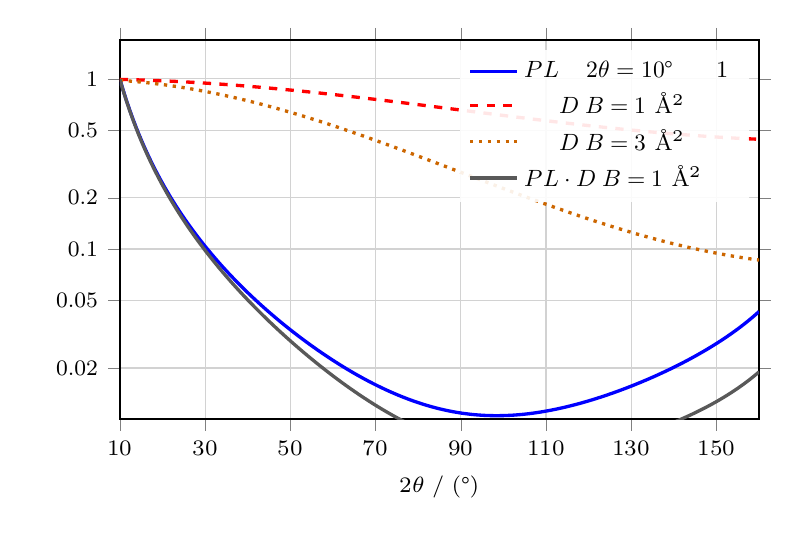
\begin{tikzpicture}
    \tikzset{declare function={
        PLf(\x) = (1+cos(\x)^2)/(4*sin(\x/2)^2*cos(\x/2));
        DWf(\x,\B) = exp(-2*\B*sin(\x/2)^2/2.3734);
      }}
    \begin{axis}[
        width=\onecolwidth, height=64mm,
        xlabel={$2\theta$ / (°)},
        ylabel={相对因子（对数纵轴）},
        xmin=10, xmax=160, ymin=0.01, ymax=1.7,
        ymode=log,
        xtick={10,30,50,70,90,110,130,150},
        ytick={0.02,0.05,0.1,0.2,0.5,1},
        yticklabels={0.02,0.05,0.1,0.2,0.5,1},
        grid=both, major grid style={gray!35}, minor grid style={gray!12},
        tick label style={font={\fontsize{8}{9.6}\selectfont}},
        label style={font={\fontsize{8}{9.6}\selectfont}},
        legend style={font={\fontsize{8}{9.6}\selectfont}, draw=none,
                      fill=white, fill opacity=0.9, text opacity=1,
                      legend cell align=left,
                      at={(0.985,0.975)}, anchor=north east},
        samples=201, domain=10:160,
      ]
      \addplot[very thick, blue] {PLf(x)/PLf(10)};
      \addlegendentry{$PL$ 因子（$2\theta=10°$ 处归一为 1）}
      \addplot[very thick, red, dashed] {DWf(x,1)};
      \addlegendentry{温度因子 $D$，$B=1$ Å$^2$}
      \addplot[very thick, orange!80!black, dotted] {DWf(x,3)};
      \addlegendentry{温度因子 $D$，$B=3$ Å$^2$}
      \addplot[very thick, black!65] {PLf(x)/PLf(10)*DWf(x,1)};
      \addlegendentry{$PL\cdot D$（$B=1$ Å$^2$）}
    \end{axis}
  \end{tikzpicture}
  \caption{两个必须做的角度修正因子随 $2\theta$ 的变化（模型计算，按式~\equref{eq:ch04b-PL}
    与式~\equref{eq:ch04b-DW}，Cu $K\alpha$，$\lambda=1.5406$ Å）。\textbf{看什么}：$PL$ 因子
    在低角极大、随角度迅速跌落（$2\theta=10°$ 处约 65，$2\theta=160°$ 处约 2.8，正好落在原书
    PL 因子图纵轴 0—80 的量程内，可作为公式重建的旁证）；温度因子在低角几乎为 1，在高角明显
    衰减，$B$ 越大衰减越强（$2\theta=160°$ 时 $B=1$ Å$^2$ 降到约 $0.44$，$B=3$ Å$^2$ 降到约
    $0.086$）。\textbf{结论}：把两条曲线相乘后，强度的角度依赖比任何单项都剧烈，因此低角与高角
    的实测强度不能直接互比，必须先做 $PL$ 与 $D$ 修正。\textbf{局限}：纵轴为对数，曲线是相对值；
    $B$ 的取值是示意（无机晶体常 $B<1$ Å$^2$，含 C、H、O、N 的有机物可到 $2$—$5$ Å$^2$）。
    \figsrc{模型计算图，非原书插图；$PL$ 的形式与原书第 246 页 PL 因子图一致。}}
  \label{fig:ch04b-pld}
\end{figure}

\begin{figure}[tbp]
  \centering
  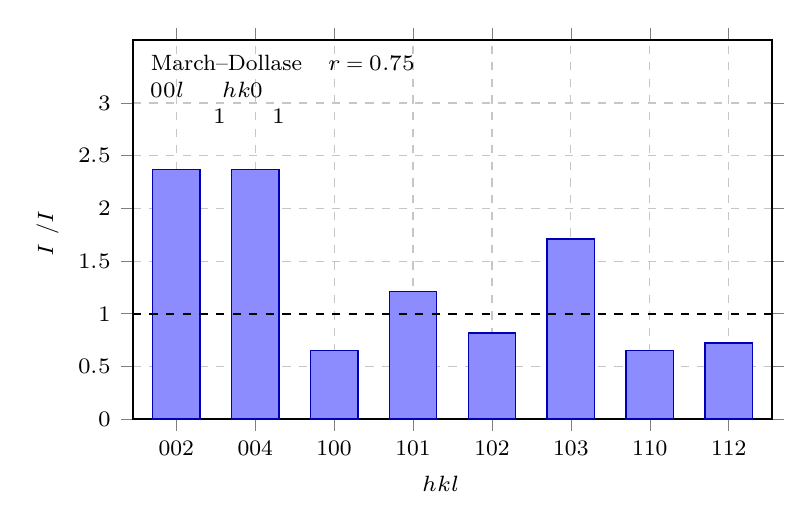
\begin{tikzpicture}
    \begin{axis}[
        width=\onecolwidth, height=64mm,
        ybar, bar width=6mm,
        xmin=0.45, xmax=8.55, ymin=0, ymax=3.6,
        xtick={1,2,3,4,5,6,7,8},
        xticklabels={002,004,100,101,102,103,110,112},
        xlabel={衍射指标 $hkl$（六方层状相模型）},
        ylabel={$I_{\text{取向}}/I_{\text{随机}}$},
        ytick={0,0.5,1.0,1.5,2.0,2.5,3.0},
        grid=major, major grid style={dashed, gray!45},
        tick label style={font={\fontsize{8}{9.6}\selectfont}},
        label style={font={\fontsize{8}{9.6}\selectfont}},
      ]
      \addplot[fill=blue!45, draw=blue!70!black] coordinates {
        (1,2.37) (2,2.37) (3,0.65) (4,1.21) (5,0.82) (6,1.71) (7,0.65) (8,0.72)
      };
      \addplot[black, thick, dashed, sharp plot, update limits=false]
        coordinates {(0.45,1) (8.55,1)};
      \node[align=left, text width=62mm, anchor=north west,
            font={\fontsize{8}{9.6}\selectfont}]
        at (axis cs:0.55,3.55)
        {March--Dollase 模型，$r=0.75$：\\ $00l$ 反射增强、$hk0$ 反射减弱，\\ 虚线为随机取向水平 $1$；
         比值偏离 $1$ \\ 完全来自制样取向，与结构无关。};
    \end{axis}
  \end{tikzpicture}
  \caption{择优取向对相对强度的影响（模型计算）。\textbf{看什么}：同一物相、同一晶胞，只改变
    晶粒取向的统计分布，相对强度就可以整体偏离随机取向的水平（虚线）达数倍，且偏离方向与
    取向方向系统的关联——层状晶粒平躺在样品面上时，反射面平行于样品面的 $00l$ 被增强，
    垂直的 $hk0$ 被减弱。\textbf{条件}：$r$ 为 March--Dollase 取向参数（$r=1$ 为随机取向），
    各峰与取向轴的夹角取 $(002,004)=0°$、$(103)=25°$、$(101)=40°$、$(102)=60°$、
    $(112)=70°$、$(100,110)=90°$；柱高为取向样品与随机取向样品的强度比。
    \textbf{局限}：这是单一取向轴的理想模型，实际样品常同时存在两种取向分量，需要用
    Rietveld 精修中的取向模型拟合，而不能靠单峰强度比判断。\figsrc{模型计算图，非原书插图。}}
  \label{fig:ch04b-texture}
\end{figure}

\begin{dataflow}
\textbf{由强度到结构信息}：实测积分强度 $\rightarrow$ 扣背底、剥离 $K\alpha_{2}$、分离重叠峰
$\rightarrow$ 除以 $PL\cdot j\cdot D\cdot A$ $\rightarrow$ 得到各峰的 $\left|F_{hkl}\right|^{2}$
$\rightarrow$ 与由结构模型（原子坐标、占位度、$B$）计算的 $\left|F_{hkl}\right|^{2}$ 比较
$\rightarrow$ 修正模型使全部峰的残差最小。注意这条链路给出的是 $\left|F\right|^{2}$ 的相对值，
只有经过标定（内标或已知结构参照）才能得到绝对尺度上的占位度。
\end{dataflow}

\begin{pitfall}
\textbf{消光是另一类使实测强度低于计算值的因素}。原消光（理想完整晶体或较大镶嵌块内部入射线
与衍射线相互干涉）与次消光（镶嵌块之间的屏蔽）都使实测强度偏低，其中原消光通常影响更大，
在晶体尺寸大、完整性好、衍射强度大且衍射角小时最严重。多晶样品晶粒小，消光比单晶法弱得多，
但\textbf{低角度强线}的实测值通常仍偏小——这正是用低角强线做定量时结果偏低的来源之一。
判别线索：计算值与实测值的偏差随强度增大、角度减小而系统增大，而不是随机分布。
\end{pitfall}

\subsubsection{原子散射因子与晶体的结构因子}

原子对 X 射线的散射源于电子散射，重元素的散射能力远高于轻原子。原子中所有电子散射的
综合效应定义为原子散射因子
\begin{equation}
f=\frac{E_{a}}{E_{e}},
\label{eq:ch04b-f}
\end{equation}
$E_{a}$ 为一个原子的散射振幅，$E_{e}$ 为一个自由电子的散射振幅。若原子的全部电子集中于一点，
则 $f$ 等于电子数 $Z$；但电子分布在核周围形成电子云，不同轨道上的电子散射波之间存在位相差，
因此一般有 $f<Z$，且随散射角增大而减小（$\theta=0$ 时无位相差，$f=Z$）。定量表达为
\begin{equation}
f\!\left(\frac{\sin\theta}{\lambda}\right)=\int_{0}^{\infty}4\pi r^{2}\rho(r)\,
\frac{\sin\!\left(4\pi r\sin\theta/\lambda\right)}{4\pi r\sin\theta/\lambda}\,dr ,
\label{eq:ch04b-fint}
\end{equation}
式中 $r$ 为电子离核距离，$\rho(r)$ 为电子云密度径向分布，$\lambda$ 为 X 射线波长。
此处已对照原页面图像（书内 p.248 / PDF p.267）：原书印为
$f=\dfrac{4\pi}{e}\displaystyle\int_{0}^{\infty}r^{2}\rho(r)\,\dfrac{\sin kr}{kr}\,dr$，
$k=\dfrac{4\pi\sin\theta}{\lambda}$，即 $4\pi r^{2}$ 权重与 $\sin x/x$ 因子、以及
$k$ 与 $\sin\theta/\lambda$ 的换算关系与原书一致。差别只在归一化前置因子：原书多一个
$1/e$（与其把 $\rho(r)$ 称作「电子云密度」并列的写法），本式按标准形式（$\rho$ 取电子数
密度，$\theta=0$ 时 $f=Z$）给出，与原书正文「当散射角 $\theta=0$……$f$ 等于电子数目 $Z$」
一致。原书同页另注：$\theta=0$ 各位相差为 $0$；$\theta\neq0$ 总有相互「抵消」，故 $f<Z$。

实际计算中不用积分式，而是用拟合多项式：以 4 组高斯项加一个常数共 9 个参数表达 $f$ 随
$\sin\theta/\lambda$ 的变化，
\begin{equation}
f\!\left(\frac{\sin\theta}{\lambda}\right)=\sum_{i=1}^{4}a_{i}\exp\!\left[-b_{i}
\left(\frac{\sin\theta}{\lambda}\right)^{2}\right]+c ,
\label{eq:ch04b-fpoly}
\end{equation}
各项系数可从《国际晶体学表》C 卷表 6.1.1.4（572—574 页）查到（已对照原页面图像，书内
p.248 / PDF p.267；原书另注该多项式由 HFS（Hartree-Fock-Slater，自洽场）法与 TFD
（Thomas-Fermi-Dirac 统计）法理论计算并结合实验数据得出，$9$ 个参数与原子或离子的电子云
分布有关；同页图 4-15 给出核外电子数均为 $10$ 的原子或离子——Si$^{4+}$、Al$^{3+}$、
Mg$^{2+}$、Na$^{+}$、Ne、F$^{-}$ 及 "Point atom"——的 $f$ 随 $\sin\theta/\lambda$ 的变化）。

由 $f$ 出发给出三条读数规律：原子散射因子随衍射角增大而减小，这是高角衍射峰减弱的重要因素；
核外电子数相等的原子实，核电荷越大、核对电子吸引越强、电子云越接近点状，$f$ 越大；同一原子
的最外层电子主要贡献低角度散射，内层电子对所有角度都有较大贡献。

晶胞的结构因子定义为晶胞内全部原子散射振幅的向量叠加：
\begin{equation}
F_{hkl}=\sum_{j=1}^{n}f_{j}\exp\!\left[2\pi i\left(hx_{j}+ky_{j}+lz_{j}\right)\right],
\label{eq:ch04b-F}
\end{equation}
$n$ 为晶胞中的原子数，$(x_{j},y_{j},z_{j})$ 为第 $j$ 个原子的分数坐标，$f_{j}$ 为其原子散射
因子。$F_{hkl}$ 既表示振幅也表示相角：写作 $F=\left|F\right|\exp(i\alpha)$，$\alpha$ 为
各原子散射波的合成相角。当晶胞为素格子且只有一个原子位于原点时 $F_{hkl}=f_{A}$，相角为零；
当格子上有两个原子且第二个位于 $(x,y,z)$ 时，二者光程差与位相差为
$\Delta=(hx+ky+lz)\lambda$、$\varphi=2\pi(hx+ky+lz)$，于是
$F_{hkl}=f_{A}+f_{B}\exp\!\left[2\pi i(hx+ky+lz)\right]$，即两个散射因子的向量加和。

在反常散射不严重时，$\left|F_{hkl}\right|=\left|F_{\bar{h}\bar{k}\bar{l}}\right|$，这就是
Friedel 定律；其结果是衍射空间的强度分布具有中心对称，$230$ 个空间群只表现出 $11$ 种
Laue 群的对称性。结构因子与晶胞内电子云密度 $\rho(x,y,z)$ 之间通过傅里叶变换联系：
\begin{equation}
F_{hkl}=\int_{V_{c}}\rho(x,y,z)\,
\exp\!\left[2\pi i(hx+ky+lz)\right]dV ,
\label{eq:ch04b-FT}
\end{equation}
反向变换给出 $\rho(x,y,z)=V_{c}^{-1}\sum_{h}\sum_{k}\sum_{l}F_{hkl}
\exp\!\left[-2\pi i(hx+ky+lz)\right]$。这一对变换关系是结构分析的基础，也解释了一个根本困难：
实测强度只给出 $\left|F_{hkl}\right|^{2}$，相角 $\alpha$ 在测量中丢失，因此“从衍射数据解结构”
的实质是先用 Patterson 法、直接法或全谱拟合（Rietveld）解决相角问题。

此处已对照原页面图像（书内 p.250 / PDF p.269）：原书正变换印为
$F_{hkl}=\int_{V}\rho(x,y,z)\exp[2\pi i(hx+ky+lz)]\,dV$，反向变换印为
$\rho(x,y,z)=\frac{1}{V}\sum_{h}\sum_{k}\sum_{l}F_{hkl}\exp[-2\pi i(hx+ky+lz)]$，
即积分在晶胞体积 $V$ 上取、微分元为 $dV$，归一化常数 $1/V$ 只出现在反向变换一侧。本式按此
改写——原稿正变换写成单位立方上的 $\int_{0}^{1}\!\!\int_{0}^{1}\!\!\int_{0}^{1}\cdots dx\,dy\,dz$，
与反向变换的 $V_{c}^{-1}$ 不属同一套归一化约定，已改成一致写法。原书同页另印出 Friedel 定律的
推导（由 $I_{hkl}=\left|F_{hkl}\right|^{2}=F_{hkl}F_{hkl}^{*}$ 与 $I_{\bar{h}\bar{k}\bar{l}}$
逐项展开相等得 $\left|F_{hkl}\right|=\left|F_{\bar{h}\bar{k}\bar{l}}\right|$），并指出衍射空间
强度分布的中心对称对应 $11$ 种 Laue 群。

\subsubsection{衍射的系统消光}

在 §4.3 的衍射几何讨论中，衍射条件由倒易格子点与 Ewald 反射球相交给出。若正空间格子为复格子，
倒易格子点会系统消失；晶体中存在螺旋轴与滑移面等微观对称元素时，也会引起衍射的系统缺失。
用式~\equref{eq:ch04b-F} 直接计算即可得到全部消光规律。

\paragraph{体心格子}晶胞中任一原子位于 $(x,y,z)$ 时，必有同种原子位于
$(x+\tfrac12,y+\tfrac12,z+\tfrac12)$。代入结构因子并提取公因子：
\begin{equation}
F_{hkl}=\sum_{j}f_{j}\exp\!\left[2\pi i(hx_{j}+ky_{j}+lz_{j})\right]
\left\{1+\exp\!\left[\pi i(h+k+l)\right]\right\}.
\label{eq:ch04b-I-extinct}
\end{equation}
当 $h+k+l=2n$（偶数）时括号内为 $2$，$F_{hkl}=2\sum_{j}f_{j}$，衍射出现；当 $h+k+l=2n+1$
（奇数）时括号内为零，$F_{hkl}=0$，衍射不出现。即体心格子的倒易格子中 $h+k+l$ 为奇数的点
全部消失——$100$、$010$、$001$ 不出现，出现的是 $200$、$020$、$002$、$110$、$101$、$011$。
该倒易格子是边长为 $2a^{*},2b^{*},2c^{*}$ 的\textbf{面心}格子。

\paragraph{面心格子}晶胞中任一原子位于 $(x,y,z)$ 时，必有另外三个原子分别位于
$(x+\tfrac12,y+\tfrac12,z)$、$(x+\tfrac12,y,z+\tfrac12)$、$(x,y+\tfrac12,z+\tfrac12)$。代入后
\begin{equation}
F_{hkl}=\sum_{j}f_{j}\exp\!\left[2\pi i(hx_{j}+ky_{j}+lz_{j})\right]
\left\{1+e^{\pi i(h+k)}+e^{\pi i(h+l)}+e^{\pi i(k+l)}\right\}.
\label{eq:ch04b-F-extinct}
\end{equation}
$h,k,l$ 全为奇数或全为偶数时 $h+k$、$h+l$、$k+l$ 均为偶数，括号内为 $4$，
$F_{hkl}=4\sum_{j}f_{j}\exp\!\left[2\pi i(hx_{j}+ky_{j}+lz_{j})\right]$，衍射出现；$h,k,l$
奇偶混杂时三个指数中一个为偶数、两个为奇数，括号内为零，衍射不出现。即面心格子的倒易格子
中 $100$、$010$、$001$、$110$、$101$ 不出现，而 $200$、$020$、$002$、$111$ 出现；其倒易格子
的基元是体心格子。类似地可证底心格子的倒易格子仍是底心格子。

\paragraph{滑移面与螺旋轴}设垂直于 $c$ 轴存在 $b$ 滑移面（设滑移面过 $z=0$），晶胞中任一原子
$(x,y,z)$ 必对应 $(x,y+\tfrac12,-z)$，代入后对 $hk0$ 指标可消去 $z$ 的影响，得到
$F_{hk0}=\sum_{j}f_{j}\exp\!\left[2\pi i(hx_{j}+ky_{j})\right]\left[1+\cos(\pi k)\right]$
（原书此处印 $1+\exp(k\pi i)$）。因此 $k=2n$ 时括号内为 $2$，衍射出现；$k=2n+1$ 时括号内为
零，$F_{hk0}=0$：倒易格子中 $hk0$ 面上 $k$ 为奇数的点全部消失。
同理，平行于 $b$ 方向存在 $2_{1}$ 螺旋轴时，$0k0$ 衍射中 $k$ 为奇数的点消失；垂直于 $b$
方向存在 $a$ 滑移面时，$(h0l)$ 中 $h=2n+1$ 的点消失；平行于 $c$ 存在 $4_{1}$ 螺旋轴时，
$00l$ 中只有 $l=4n$ 的点存在。此处已对照原页面图像（书内 p.252—253 / PDF p.271—272）：
滑移面一段原书取原子对 $(x,y+\tfrac12,-z)$（滑移面过 $z=0$），$2_{1}$ 螺旋轴一段原书取
$(-x,y+\tfrac12,-z)$（螺旋轴过 $x=0,z=0$），结论均为对应指标中奇数的点消失。原书在同节
末尾以三条结论归纳：P 格子且无螺旋轴、滑移面等微观对称元素时衍射谱无任何系统消光；复格子
使某些 $hkl$ 系统消光但不破坏倒易格子特性；螺旋轴与滑移面使倒易格子出现「空位缺陷」，
并明确举出垂直于 $b$ 的 $a$ 滑移面使 $(h0l)$ 中 $h=2n+1$ 消失、平行于 $c$ 的 $4_{1}$
螺旋轴使 $00l$ 中仅 $l=4n$ 存在。

\begin{table}[tbp]
  \centering
  \caption{点阵类型与微观对称元素引起的系统消光规律。表中“出现条件”是对该组衍射指标而言，
    其余指标不受此条限制。\src{据 S1（上册）§4.4.4，书内 p.250—253 / PDF p.269—272 归纳。}}
  \label{tab:ch04b-extinction}
  \begin{tabular}{@{}lll@{}}
    \toprule
    类型 & 出现（衍射）条件 & 系统消光 \\
    \midrule
    简单格子 $P$ & 无附加条件 & 无消光，全部 $hkl$ 出现 \\
    体心 $I$ & $h+k+l=2n$ & $h+k+l$ 为奇数 \\
    面心 $F$ & $h,k,l$ 全奇或全偶 & $h,k,l$ 奇偶混杂 \\
    底心 $C$ & $h+k=2n$ & $h+k$ 为奇数 \\
    $b$ 滑移面 $\perp c$ & $hk0$ 中 $k=2n$ & $hk0$ 中 $k$ 为奇数 \\
    $a$ 滑移面 $\perp b$ & $h0l$ 中 $h=2n$ & $h0l$ 中 $h$ 为奇数 \\
    $2_{1}$ 螺旋轴 $\parallel b$ & $0k0$ 中 $k=2n$ & $0k0$ 中 $k$ 为奇数 \\
    $4_{1}$ 螺旋轴 $\parallel c$ & $00l$ 中 $l=4n$ & $00l$ 中 $l\neq4n$ \\
    \bottomrule
  \end{tabular}
\end{table}

\begin{keycond}
三类信息可以直接由“哪些峰存在”读出：点阵类型（复格子）使\textbf{整类}衍射指标消失，倒易
格子的格子型式甚至基本矢量发生改变而不破坏格子特性；螺旋轴与滑移面使\textbf{某条直线或某个面}
上的格子点部分消失，相当于在倒易格子里出现“空位缺陷”。因此，衍射谱上峰的“有无规律”是点阵
类型与可能空间群的直接证据，与峰位、峰强构成相互独立的三重校验。反过来，若一套指标化结果
不能给出任何系统消光规律，其可靠性就要打折扣（见 §4.6.4）。
\end{keycond}

\begin{methodsum}
本章主线可以压缩成三句话：\textbf{峰位 $\rightarrow$ 晶胞}（由 $2\theta$ 得 $d$、$Q$，解出晶胞
参数与点阵对称性）；\textbf{峰强 $\rightarrow$ 晶胞内原子分布}（由修正后的 $\left|F_{hkl}\right|^{2}$
得到原子种类、坐标、占位度与热振动）；\textbf{峰的有无 $\rightarrow$ 点阵类型与微观对称元素}
（系统消光定格子类型、滑移面与螺旋轴）。三者的关系是：布拉格方程给出衍射出现的必要条件，
结构因子不为零才是充分条件。\src{书内 p.253—254 / PDF p.272—273}
\end{methodsum}

\subsection{物相鉴定与相定量分析}
\src{上册 §4.5，书内 p.254—264 / PDF p.273—283}

\subsubsection{物相定性分析}

\begin{probout}
\textbf{测什么}：把实测 $d$—$I/I_{1}$ 数据组与标准卡片比对，确定样品由哪些晶相组成。\\
\textbf{能推断什么}：某物相\textbf{存在}（当其特征线全部出现且相对强度合理时），以及通过
与已知结构对比给出晶型是否相同的判断。\\
\textbf{不能推断什么}：某物相\textbf{不存在}。含量低或衍射能力弱时其特征线显示不出来，
因此该方法只能确定某相存在，不能确定某相绝对不存在；含量低于约 $3\%$ 的物相通常很难鉴定出来，
若某物相全部由轻原子（C、H、O、N）组成而其他相含重原子，即使含量到 $40\%$ 也可能鉴别不出来。
\src{书内 p.258 / PDF p.277}
\end{probout}

\begin{principle}
物相定性的依据有两条。第一，任何一种结晶固体都有自己独立的一套衍射图谱，峰位与强度完全
取决于其内部结构：由式~\equref{eq:ch04b-Q}，晶胞参数不同则 $d$ 不同、衍射角不同；由
式~\equref{eq:ch04b-F}，各峰强度由晶胞中原子分布方式决定。因此每种晶态物质的衍射图谱与其
结构之间存在一一对应关系。第二，物质不会因为与其他物质混合而改变自己的衍射行为——混合物中
各物相的衍射互不干扰，混合物的图谱是各组成物相图谱的简单叠加。这两条合起来就是“用图谱
鉴别晶态物质”的全部依据。
\end{principle}

\begin{measure}
标准数据的形式与检索方式决定了物相分析的工作流程。1938 年 Hanawalt 等人用 $d$—$I$ 数据组
代替衍射图制作卡片；1942 年美国测试与材料协会将数据汇编成 1300 张卡片出版，简称 ASTM 卡片；
1972 年后由粉末衍射标准联合委员会（JCPDS）编辑出版，称 JCPDS 卡（PDF 卡）；现在由国际衍射
数据中心（ICDD）发行，简称 ICDD 卡。卡片按区域分载：卡片号（组号 + 卡号）、该相三强线及第一个
峰的 $d$ 值与相对强度、化学式与英文名称、数据可靠度符号（用星号标记者表示数据非常可靠，
$i$ 表示比较可靠，空白表示可靠性一般，$O$ 表示可靠性差，$C$ 表示由晶体结构数据计算得到，个别卡片为 $R$ 表示来自 Rietveld 精修结果）、
实验条件（辐射种类 $\mathrm{Rad}$、波长 $\lambda$、滤波片 $\mathrm{Filter}$、相机直径
$\mathrm{Dia}$、测量方法、参考文献）、晶体学数据（晶系 $\mathrm{sys}$、空间群 $\mathrm{S.G}$、
晶胞参数、计算密度 $D_{x}$、晶胞中化学式单位数 $Z$）、物性数据、以及全部 $d$—$I$—$hkl$ 数据
（强度以最强峰 $I_{1}=100$ 归一）。\\
检索工具有两类：\textbf{字母索引}（Davey 索引，按物相英文名称字母顺序，条目含名称、化学式、
三强线 $d$ 值与相对强度、卡片号、参比强度）最常用，适用于已知化学组成、能估计可能物相的样品；
\textbf{数字索引}（Hanawalt 索引，按最强线的 $d$ 值由大到小分 87 组，组内按第二、第三个 $d$ 值
依次排列，且前三条线的 $d$ 值轮流占据首位，因此同一张卡片在索引中出现三次）适用于物相或元素
完全未知的样品。
\end{measure}

\begin{dataflow}
（1）按要求制样并获得衍射数据；（2）由峰位按布拉格方程计算 $d$ 值，读取强度并计算相对强度
$I/I_{1}$；（3）用字母或数字索引检索 PDF 卡片；（4）与候选卡片逐线比对，判定唯一合理的 PDF
卡片。比对时允许实测 $d$ 与卡片 $d$ 存在差异，原书举例如下：$d\sim1$ Å 时允许 $\pm0.003$ Å、
$d\sim3.5$ Å 时允许 $\pm0.03$ Å、$d\sim8$ Å 时允许 $\pm0.25$ Å；误差在此范围内即视为相符。
（此处已对照原页面图像（书内 p.257 / PDF p.276）：原书三档误差都给出了对应的 $d$ 值，即
$1$ Å、$3.5$ Å、$8$ Å；本节此前只写“更高角度允许 $\pm0.25$ Å”，未指认其适用的 $d$ 范围。）
实验时要注意温度与仪器零点的影响，消除仪器误差可加内标物（如 \ce{SiO2}、\ce{CaF2}）。
\end{dataflow}

\begin{pitfall}
\textbf{（1）把 $d$ 值符合与强度符合的权重搞反。}实测数据与 PDF 卡片通常不完全一致；
比对时 $d$ 值的符合比相对强度的符合更重要，相对强度只作参考。\\
\textbf{（2）忽略低角区与高角区的信息量差异。}不同晶体在低角度 $d$ 值一致的机会很少，而在高角度
不同晶体间衍射峰相似的机会较大。因此低角区衍射与卡片数据的符合比高角区的符合更重要。\\
\textbf{（3）把重叠峰当成某相的强线。}多相混合样品中不同相的某些衍射峰可能互相重叠，某些“强线”
实际上并不是某一物质的强衍射；若以它作为最强线去检索，很难得到符合的结果。\\
\textbf{（4）忽略仪器分辨率与样品位移对“匹配”的影响。}不同仪器（狭缝、测角仪半径、光源）给出的
峰宽与峰形不同，样品位移还会使全部峰位同向偏移。若把 PDF 卡片当成“精确到小数点后三位就必须
逐位对上”的标尺，会做出错误排除或错误匹配。正确做法：先用内标校正峰位，再按 $d$ 值的角度分段
容差比对，并优先信任低角线。\\
\textbf{（5）结构相似相之间的误判。}有些物质结构相似，仅点阵常数差别不大、原子散射能力也相近，
衍射峰差别很小，必须与化学分析、电子探针、能谱等方法结合才能得出正确结果。\\
\textbf{（6）忽略卡片版本。}不同编号的同一物质卡片，应以发表较晚卡片上的数据为准。
\end{pitfall}

\begin{crosscheck}
物相鉴定不应单独成立：应与化学分析、X 射线荧光（元素组成）、光谱、电子探针与能谱（微区成分）
互相配合。若物相太多、衍射线重叠严重，可用重力、磁力等方法先把某些物相富集或分离，再分别鉴定。
鉴定结论还应与样品来源或制备方法一致——例如由硝酸盐分解制备的样品中出现对应的氧化物相是合理的，
出现无关的硅酸盐相则需要解释来源。
\end{crosscheck}

\subsubsection{物相定量分析}

\begin{probout}
\textbf{测什么}：各晶相在样品中的相对含量（质量分数）。\\
\textbf{前提}：物相定性分析是相定量的出发点——只有先确认样品中含有指定物相，相定量才有意义。\\
\textbf{能推断什么}：晶相之间的相对比例，精度通常到百分之一到百分之几。\\
\textbf{不能推断什么}：不能直接给出非晶相的含量，也不能在未做标定的情况下给出绝对含量。
\end{probout}

\begin{principle}
由式~\equref{eq:ch04b-intensity}，对选定 $hkl$ 的衍射峰，$\left|F_{hkl}\right|^{2}$、$j$、$D$
以及与角度相关的 $P$、$L$ 都是确定值，强度仅是样品受照射有效体积 $\Delta V$ 的函数，可把确定
的项合并为常数：$I=K\Delta V$。采用 Bragg--Brentano 衍射仪、平板样品时
$\Delta V=A_{0}/(2\mu_{l})$，故 $I=KA_{0}/(2\mu_{l})$，其中 $\mu_{l}$ 为线吸收系数，
$A_{0}$ 为入射线垂直截面积。\textbf{衍射仪做相定量的最大便利正在于此：吸收效应不随 $\theta$
改变，易于校正。}\\
多相体系中各相独立产生衍射，混合体系可看作各单相体系的体积权重加和。设 $i$ 相的体积分数为
$v_{i}$、质量分数为 $w_{i}$，总线吸收系数 $\mu_{l}=\sum_{i}v_{i}\mu_{l,i}$，则
\begin{equation}
I_{i}=\frac{K_{i}v_{i}}{\mu_{l}} .
\label{eq:ch04b-Ii-V}
\end{equation}
改用质量吸收系数 $\mu_{m}$（$\mu_{l}=\rho\mu_{m}$，$\rho$ 为样品密度；$\mu_{m}$ 只与组成元素及
其质量分数有关，与聚集状态无关，故同分异构体的多相体系 $\mu_{m}$ 是常数）：
\begin{equation}
\mu_{m}=\sum_{i}w_{i}\mu_{m,i},\qquad
I_{i}=\frac{k_{i}w_{i}}{\mu_{m}},\qquad k_{i}=\frac{K_{i}}{\rho_{i}} .
\label{eq:ch04b-Ii-w}
\end{equation}
式~\equref{eq:ch04b-Ii-w} 是 X 射线相定量分析最基本的公式，以下各种方法都从它出发；各方法的
差别只在于如何计算或消去常数 $k_{i}$ 与总质量吸收系数 $\mu_{m}$。
（此处已对照原页面图像（书内 p.259—260 / PDF p.278—279）：原书由单相式 $I=K\Delta V$ 与
Bragg-Brentano 有效体积 $\Delta V=A_{0}/(2\mu)$ 得 $I_{i}=K_{i}v_{i}/\mu_{t}$（$\mu_{t}$ 为总线
吸收系数），再由 $v_{i}=V_{i}/V_{t}=w_{i}\mu_{t}/(\rho_{i}\mu_{mt})$ 过渡到质量分数，得
\[ I_{i}=\frac{K_{i}}{\rho_{i}}\cdot\frac{w_{i}}{\mu_{mt}}, \]
即本式——$\rho_{i}$ 与 $K_{i}$ 同处分子，故 $k_{i}=K_{i}/\rho_{i}$ 确为合并写法。符号差异：原书总线
吸收系数与总质量吸收系数记作 $\mu_{t}$、$\mu_{mt}$，本节沿用 $\mu_{l}$、$\mu_{m}$；原书未印
$\mu_{m}=\sum_{i}w_{i}\mu_{m,i}$ 的质量加权求和式，只印 $\mu_{mt}\rho_{t}=\mu_{t}=\sum_{i}v_{i}\mu_{i}$，
两者等价。）
\end{principle}

\paragraph{外标法}若多相体系中各相化学组成相同而结构不同（同分异构体混合物），则 $\mu_{m}$ 是
常数、不随各组分质量分数改变，于是相同实验条件下纯 $i$ 相该峰的强度 $I_{i}^{0}$ 与混合样品中
的强度之比直接给出含量：
\begin{equation}
w_{i}=\frac{I_{i}}{I_{i}^{0}} .
\label{eq:ch04b-external}
\end{equation}
外标法原理简单，但局限性大：只适用于上述有限体系（$\mu_{m}$ 恒定），需要纯物质作外标物，
且必须严格控制实验条件——制样条件（样品处理、压样用力）平行、仪器稳定，通常需要多次制样与
测试以检验强度的重复性。

\paragraph{内标法}对 $n>2$ 相体系，各组分 $\mu_{m,i}$ 不同，$\mu_{m}$ 随组成变化，
式~\eqref{eq:ch04b-external} 不再成立。此时在样品中定量加入一种原体系不含的标准物质 $s$ 相。
设原体系在新混合体系中的质量分数为 $w_{0}$，$i$ 相与原体系的质量分数分别为 $w_{i}$、$w_{s}$，
则 $i$ 相在新体系中的质量分数 $w_{i}'=w_{i}w_{0}$。将 $i$ 相与 $s$ 相的强度公式相除，总质量
吸收系数被消去：
\begin{equation}
\frac{I_{i}}{I_{s}}=K\frac{w_{i}'}{w_{s}},\qquad w_{i}=\frac{w_{i}'}{w_{0}}=\frac{w_{i}'}{1-w_{s}} .
\label{eq:ch04b-internal}
\end{equation}
即 $i$ 相与内标相的强度比与其在新混合体系中的含量成正比。实际工作中配制一系列 $i$ 与 $s$ 含量
已知的样品，测强度比作工作曲线，由斜率求 $K$，再算出 $w_{i}'$ 并推回原体系的 $w_{i}$。
内标物的选择条件：测试峰与待测组分峰尽量靠近但不重叠、也不与其他峰重叠；峰强度足够高；
结晶完整性高、无择优取向（一般优先选立方晶系物质）；性质稳定，X 射线照射下不变、不与样品
起化学反应。内标法所得校正曲线适用于任何含待测物相的多相体系，只要求用相同内标物与相同衍射峰；
若校正曲线所用峰在样品中与其他组分重叠，可另选新峰，通过新峰与原峰积分强度之比对各点乘以该
比值即可换算曲线，不必重做实验。

\paragraph{参比强度法（RIR／$K$ 值法）}参比强度法是内标法的发展，本质仍是内标法，区别在于
\textbf{统一了参比物}：以刚玉（corundum，$\alpha$-\ce{Al2O3}，$R\bar{3}c$）为通用参考标准，
取刚玉 $(113)$ 衍射峰为参比峰，定义待测相 $i$ 与刚玉按质量比 $1:1$ 混合时二相最强线的强度比
为该相的参比强度 $K_{i}$。当体系中原有的 $n$ 相之外加入定量内标物 $f$ 时，
\begin{equation}
\frac{I_{i}}{I_{f}}=\frac{K_{i}}{K_{f}}\cdot\frac{w_{i}}{w_{f}},
\label{eq:ch04b-RIR}
\end{equation}
即体系中任意二组分的强度比正比于二组分的浓度比，比例系数等于二组分参比强度之比，\textbf{与样品中
其他组分的存在无关}。因此只要在同一扫描中测出待测相峰与内标物峰的强度比，配合参比强度与内标物
加入量即可算出含量，\textbf{不必再做校正曲线}——内标物在这里起的是“冲洗剂”的作用，故也称基体
冲洗法。1972 年之后 JCPDS 卡片直接给出部分物质与刚玉相比的参比强度值；使用卡片值时必须注意
仪器条件与样品状况，必要时自行测定。若以刚玉为内标物加入 $n$ 组分体系，且令 $K_{f}=K_{c}=1$，
公式进一步简化为 $I_{i}/I_{c}=K_{i}w_{i}/w_{c}$，即 $w_{i}=w_{c}I_{i}/(K_{i}I_{c})$。

\paragraph{自动冲洗绝热法（无标法）}在 $n$ 相体系中不加内标物，仅从一张衍射图求各相含量。
其原理与参比强度法相同：任意两相之间 $I_{i}/I_{j}=(K_{i}w_{i})/(K_{j}w_{j})$，对 $n$ 相体系可写
出 $n(n-1)/2$ 个方程，其中独立方程数为 $n-1$，加上归一化条件 $\sum_{i}w_{i}=1$ 正好有 $n$ 个
独立方程。由此得
\begin{equation}
w_{i}=\frac{I_{i}/K_{i}}{\sum_{j=1}^{n}I_{j}/K_{j}} .
\label{eq:ch04b-flushing}
\end{equation}
若混合样中各组分都是可结晶物质且都有已知的 $K_{i}$，则无需加入冲洗剂即可直接计算各组分含量。
\textbf{但当样品中存在无定形（非晶）物质时，该公式不能应用}，只能向样品中加入内标物处理——
原因很简单：非晶相不产生布拉格峰，$\sum w_{i}=1$ 的归一化假设被破坏，算出的各晶相含量会被系统性
高估。
（此处已对照原页面图像（书内 p.263 / PDF p.282）：原书由参比强度法关系
$I_{1}/I_{i}=(K_{1}/K_{i})(w_{1}/w_{i})$（$i=1,2,\cdots,n$）出发，指出 $i=1$ 的方程是恒等式、非独立
方程；改写为 $w_{i}=(I_{i}/K_{i})(K_{1}/I_{1})w_{1}$ 后代入归一化方程 $\sum_{i}w_{i}=1$，得
$w_{1}=\left(\frac{K_{1}}{I_{1}}\sum_{i=1}^{n}\frac{I_{i}}{K_{i}}\right)^{-1}$，对体系中任意一相 $i$ 即
$w_{i}=\left(\frac{K_{i}}{I_{i}}\sum_{j=1}^{n}\frac{I_{j}}{K_{j}}\right)^{-1}$，与式~\equref{eq:ch04b-flushing}
互为倒数写法、代数等价。原书同页明确「原理上，自动冲洗绝热法与参比强度法相同」，各组分「均有已知的
参比强度 $K_{i}$ 值」，故 $K_{i}$ 即参比强度；「当样品中有无定形物质存在时，就不能应用这个公式来计算」
与本段末句一致。）

\begin{table}[tbp]
  \centering
  \caption{四类相定量方法的适用差别。选择方法的第一步是判断“总质量吸收系数是否随组成变化”，
    第二步是判断“能否接受加入内标物”。\src{据 S1（上册）§4.5.2，书内 p.258—264 / PDF p.277—283 归纳。}}
  \label{tab:ch04b-quantmethods}
  \begin{tabular}{@{}p{21mm}p{42mm}p{33mm}p{38mm}@{}}
    \toprule
    方法 & 适用体系与前提 & 标样与工作曲线 & 主要误差来源 \\
    \midrule
    外标法 & 各相化学组成相同、结构不同（同分异构体）；$\mu_{m}$ 恒定 &
    需纯 $i$ 相作外标；需严格控制制样与仪器条件，常需多次重复 &
    制样平行性、压样用力、仪器漂移；适用范围窄 \\
    内标法 & 任意 $n$ 相体系（$n>2$）；可加入原体系不含的 $s$ 相 &
    需选合格内标物；需配制系列样品作工作曲线 &
    内标物纯度与加入量准确性、混合均匀性、峰重叠 \\
    参比强度法（RIR／$K$ 值） & 任意多相体系；本质是内标法 &
    以刚玉 $(113)$ 峰为统一参比；可用卡片 $K_{i}$ 值，\textbf{不必做工作曲线} &
    卡片 $K_{i}$ 值与本机条件不匹配、择优取向、峰重叠 \\
    自动冲洗绝热法 & 各相均可结晶、均有已知 $K_{i}$ 的多相体系；\textbf{不能含非晶相} &
    无需内标物、无需工作曲线，仅用一张衍射图 &
    存在非晶相时归一化失效、$K_{i}$ 值误差直接传递、重叠峰 \\
    \bottomrule
  \end{tabular}
\end{table}

\begin{measure}
相定量的实验要点：（1）样品尽可能细，粒度通常要小于 $15$\,µm，并尽可能消除择优取向；
（2）合理选择衍射条件——管压、管流、狭缝、扫描速度、扫描区间，数据处理要审慎，必要时重复测试；
（3）\textbf{峰强用积分强度且计数要足够}；若用峰高代替积分强度，要注意仪器型号与实验条件——
同型号仪器的峰高／峰宽比随 $2\theta$ 的变化相同，不同型号仪器则不同，因此用峰高得到的校正曲线
只能在同一型号仪器上通用，用积分强度得到的校正曲线则可在不同型号仪器上通用；若待测组分晶粒
尺寸在 $100$ nm 以下且各样品的晶粒大小不一致，则不能用峰高代替积分强度；（4）相定量的灵敏度
约为 $5\%$：含量较高时一般可确认该物相存在，含量很低或无法给出时，需要结合样品来源或制备
方法、化学分析及其他表征数据综合判断。\src{书内 p.264 / PDF p.283}
\end{measure}

\begin{pitfall}
\textbf{定量误差主要来自三处。}\\
\textbf{（1）择优取向（最常被低估的一项）。}层状、针状、片状晶粒在压片时趋于定向排列，使
反射面平行于样品面的衍射峰被增强、垂直的被减弱（图~\figref{fig:ch04b-texture}）。由于各相的
取向程度不同，相与相之间的强度比不再正比于含量比，误差可达数十个百分点。抑制办法：减小粒度、
侧装或轻压、加冲淡剂（如与样品吸收系数接近的稀释剂）、必要时用取向函数在 Rietveld 精修中校正。\\
\textbf{（2）微吸收。}颗粒尺寸与吸收系数不匹配时，X 射线在单个颗粒内被吸收，颗粒内部的散射
被屏蔽，导致“强度—含量”偏离线性。颗粒越粗、各相吸收系数差别越大，偏差越严重；吸收系数大
的相（含重原子）在粗颗粒状态下其强度会被系统性压低。判据是颗粒线度应远小于 $1/\mu_{l}$；
否则需减小粒度或按 Brindley 方法做微吸收校正。\\
\textbf{（3）非晶相未计入。}自动冲洗绝热法（以及一切用 $\sum w_{i}=1$ 归一的方法）以“全部
物质都产生布拉格峰”为前提。催化剂、玻璃、无定形碳、无定形载体上负载的活性相都含有非晶成分，
此时归一化把非晶部分的质量摊给了各晶相，\textbf{各晶相含量被系统性高估}，而且高估比例随非晶
含量增大而增大。正确做法是加入内标物，由内标相的含量反推非晶相的总量，再换算各晶相在原样品
中的绝对含量。\\
此外还有两项次要但常被忽略的来源：峰重叠未分离（把重叠峰强度全部计入某一相）、以及用峰高
代替积分强度（图~\ref{fig:ch04b-pld} 所示的角度依赖使峰宽随 $2\theta$ 变化，峰高比不再正比于
积分强度）。
\end{pitfall}

\begin{crosscheck}
相定量结果应与独立方法互校：热分析（灼烧失重、结晶水）、元素分析（化学法或 XRF）给出元素
总量约束；Rietveld 全谱拟合给出包含结构信息的相含量（见后续分片）；把内标法与参比强度法
并行做一次，若两者相差超过预期误差，问题通常出在择优取向或非晶相未计入，而不是在计算方法上。
\end{crosscheck}

\subsection{衍射图的指标化}
\src{上册 §4.6，书内 p.264—269 / PDF p.283—288}

\begin{probout}
\textbf{测什么}：为多晶衍射图中的每一条衍射线指定衍射指标 $hkl$。\\
\textbf{能推断什么}：由
\begin{equation}
Q_{hkl}=f\left(h,k,l;a,b,c,\alpha,\beta,\gamma\right)
\label{eq:ch04b-indexbase}
\end{equation}
反解出晶胞参数 $(a,b,c,\alpha,\beta,\gamma)$，实现倒易点阵的重建；同时得到晶体所属晶系、点阵
类型与可能的空间群等信息。用一套晶胞参数指标化全部衍射线，是确认样品为单相的重要依据；
把指标化所得的晶胞参数、样品实际组成与已知结构的原子参数结合起来计算衍射图并与实验图对照，
可以判明样品是否与已知化合物具有相同晶型。\\
\textbf{困难在哪}：$n$ 条线只有 $n$ 个方程，一般晶系含 $3n+6$ 个未知数（即使对称性最高的立方
晶系也有 $3n+1$ 个），从数学上看指标化是一个“无解”的难题；出路在于衍射指标只能取整数，
且低角度区域首先出现指标低的衍射峰——指标化因此是尝试与推理结合的过程，本质上是\textbf{多解}
问题。\src{书内 p.264—265 / PDF p.283—284}
\end{probout}

\subsubsection{立方晶系指标化方法：解析法}

立方晶系只有一个晶胞参数需要确定，不同衍射峰的 $Q$ 值之间存在完全由整数指标决定的比例关系：
\begin{equation}
\frac{Q_{i}}{Q_{1}}=\frac{h_{i}^{2}+k_{i}^{2}+l_{i}^{2}}{h_{1}^{2}+k_{1}^{2}+l_{1}^{2}} .
\label{eq:ch04b-cubicratio}
\end{equation}
由于指标只能取整数且以平方和的形式出现，只需按 $0,1,2,3,\dots$ 从小到大组合 $h,k,l$，依次得到
$100$、$110$、$111$、$200$、$210$、$211$、$220$、$300$、$310$、$311$、$222$、$320$、
$321$、$400$、$410$、$322$、$411$、$330$、$331$、$420$ 等，再按系统消光规律剔除不出现的指标，
即可得到 $Q$ 比值序列：

（1）\textbf{简单立方}：$Q$ 比值 $1:2:3:4:5:6:8:9:10:11:12:13:14:16:17:18\cdots$，
其中缺失 $7$ 和 $15$（$h^{2}+k^{2}+l^{2}$ 不能等于 $7$ 或 $15$）。\\
（2）\textbf{体心立方}：只有 $h+k+l=2n$ 的衍射出现，$Q$ 比值
$2:4:6:8:10:12:14:16:18:20\cdots$，化为最简后即 $1:2:3:4:5:6:7:8:9:10\cdots$，\textbf{所有整数
都出现}（比值 $7$ 出现，这是与简单立方的关键差别）。\\
（3）\textbf{面心立方}：$h,k,l$ 奇偶混杂的衍射消光，$Q$ 比值
$3:4:8:11:12:16:19:20:24:27\cdots$，呈现疏密交替的衍射花样——这也是面心立方粉末图最直观的
识别特征。（此处已对照原页面图像（书内 p.265 / PDF p.284）：原书三式分别只印到
$1:2:3:4:5:6:8:9:10:11:12:13:14:16:17:18\cdots$（并注明缺失 $7$ 和 $15$）、
$2:4:6:8:10:12:14:16:18:20\cdots$（化简后为 $1:2:3:4:5:6:7:8:9:10\cdots$，并注明其中出现 $7$）
与 $3:4:8:11:12:16:19:20\cdots$，三式均以省略号收尾；本序列续列的 $24$、$27$ 等项是按
$h^{2}+k^{2}+l^{2}$ 的可能取值与系统消光条件补出的，不是原书印出的项。）

\begin{keycond}
立方晶系多晶衍射数据指标化的一般步骤（原书五步，此处给出每步的判据与常见失误）：
（1）读出各衍射峰的 $2\theta$，由布拉格方程 $\sin\theta=\lambda/(2d)$ 计算 $\sin^{2}\theta$
（同一辐射源下 $\sin^{2}\theta$ 的比值与 $Q$ 的比值相同），按由小到大排列；
（2）计算各 $\sin^{2}\theta$ 与最小 $\sin^{2}\theta$ 的比值；
（3）若比值都接近整数则化为整数；若有的比值不接近整数，观察数值关系乘以适当的整数（$2$、$3$、
$\dots$）使全部比值接近整数并进一步化简——这一步是立方解析法的关键，也是产生“晶胞体积
亚倍／倍数假解”的地方；
（4）根据比值关系判断格子类型，确定各衍射峰的指标 $hkl$；
（5）由布拉格方程计算各峰的 $d$ 值，进而计算晶胞参数 $a$。
\textbf{判据}：第（4）步得到的格子类型必须与该相已知的消光规律（表~\tabref{tab:ch04b-extinction}）
一致；第（5）步中各条线单独算出的 $a$ 应当在误差范围内一致，若 $a$ 随角度系统漂移，说明峰位
未做位移校正或指标化有误。
\end{keycond}

\begin{example}[面心立方相的指标化（模型数据）]
以下为一组自洽的模型数据（$a=4.078$ Å，Cu $K\alpha$，$\lambda=1.5418$ Å，由
$\sin^{2}\theta=(\lambda^{2}/4a^{2})N$ 正算得到），用来演示上节五步：
\begin{center}
\begin{tabular}{@{}ccccc@{}}
  \toprule
  $2\theta$ / (°) & $\sin^{2}\theta$ & 比值（$\times3$） & $N=h^{2}+k^{2}+l^{2}$ & $hkl$ \\
  \midrule
  38.22 & 0.1072 & 3 & 3 & 111 \\
  44.42 & 0.1429 & 4 & 4 & 200 \\
  64.63 & 0.2859 & 8 & 8 & 220 \\
  77.66 & 0.3931 & 11 & 11 & 311 \\
  81.80 & 0.4288 & 12 & 12 & 222 \\
  98.24 & 0.5718 & 16 & 16 & 400 \\
  111.02 & 0.6790 & 19 & 19 & 331 \\
  115.40 & 0.7147 & 20 & 20 & 420 \\
  \bottomrule
\end{tabular}
\end{center}
\vspace{0.3em}
（1）由 $2\theta$ 算出 $\sin^{2}\theta$ 并升序排列；（2）与最小值 $0.1072$ 相比得
$1:1.333:2.667:3.667:4:5.333:6.333:6.667$，都不是整数；（3）观察数值关系，乘以 $3$ 后得
$3:4:8:11:12:16:19:20$——全部为整数，且不含 $3:1$ 的简单比例（说明最小线不是 $100$），
序列表中缺失 $5,6,7,9,10$ 等值；（4）该序列正是面心立方的特征序列（最小 $N=3$ 对应 $111$），
据此判定格子类型为面心立方并指定上表指标；（5）由
$a=\lambda\sqrt{N}/(2\sin\theta)$ 逐线计算，八条线一致给出 $a=4.078$ Å（高角线权重更大，
因为 $\Delta d/d$ 随 $\theta$ 增大而减小）。
\textbf{本例的用途}：它演示了“比值 $\rightarrow$ 整数化 $\rightarrow$ 消光判据 $\rightarrow$ 指标”
这一完整链条；若在第（3）步只乘到 $1$ 而不乘 $3$，就会得到 $1:1.33:2.67\cdots$ 的“非整数序列”
而误判为不合格数据。
\end{example}

\subsubsection{Hesse--Lipson 解析法}

\begin{principle}
Hesse--Lipson 法适用于四方、六方与正交晶系，思路仍是利用晶体周期性结构决定的衍射峰之间的
变化关系。以正交晶系（三个待定参数）为例，把布拉格方程代入 $\sin^{2}\theta$ 得
\begin{equation}
q_{hkl}\equiv\sin^{2}\theta_{hkl}
=\frac{\lambda^{2}}{4}\left(\frac{h^{2}}{a^{2}}+\frac{k^{2}}{b^{2}}+\frac{l^{2}}{c^{2}}\right)
=A h^{2}+B k^{2}+C l^{2},\qquad
A=\frac{\lambda^{2}}{4a^{2}},\;B=\frac{\lambda^{2}}{4b^{2}},\;C=\frac{\lambda^{2}}{4c^{2}} .
\label{eq:ch04b-HL}
\end{equation}
这里的待定量是 $q=\sin^{2}\theta$，\textbf{不是}倒易量 $Q=1/d^{2}$，两者只差一个常数因子
$q=(\lambda^{2}/4)Q$：相减与相除时该因子都会约去，所以下面的差值关系对二者同样成立，但
$A,B,C$ 的数值必须与反算公式配套——本节取 $A=\lambda^{2}/(4a^{2})$，反算用
$a=\lambda/(2\sqrt{A})$、$b=\lambda/(2\sqrt{B})$、$c=\lambda/(2\sqrt{C})$（若改按
$Q=1/d^{2}$ 记账，系数就是 $1/a^{2}$、反算 $a=1/\sqrt{A}$，两套不能混用）。
于是“有关联但指标不同”的 $q$ 值之间存在严格的加和与倍数关系，例如
$q_{hkl}=q_{h00}+q_{0k0}+q_{00l}$，$q_{200}=4q_{100}$，$q_{300}=9q_{100}$，
$q_{hk0}=q_{h00}+q_{0k0}$ 等。\textbf{这些关系就是该方法的全部依据}：只要能从实测数据中识别出
哪些差值对应轴面衍射，三个参数就被确定（正交晶系要三条互不成比例的线才能定出 $A,B,C$
三个独立系数）。
（此处已对照原页面图像（书内 p.266 / PDF p.285）：原书即令 $q_{hkl}=\sin^{2}\theta_{hkl}$，
并把正交晶系的方程变换为 $q_{hkl}=\sin^{2}\theta=Ah^{2}+Bk^{2}+Cl^{2}$，其中
$A=\lambda^{2}/4a^{2}$、$B=\lambda^{2}/4b^{2}$、$C=\lambda^{2}/4c^{2}$，与本式一致；原书同页给出的
加和与倍数关系为 $q_{hkl}=q_{h00}+q_{0k0}+q_{00l}=q_{hk0}+q_{00l}=q_{h0l}+q_{0k0}=\cdots$ 及
$q_{1kl}-q_{0kl}=q_{100}$、$q_{2kl}-q_{0kl}=4q_{100}$、$q_{3kl}-q_{0kl}=9q_{100}$，
本式所写的 $q_{200}=4q_{100}$、$q_{300}=9q_{100}$ 是其在 $k=l=0$ 时的特例。原书未另行定义
倒易量 $Q=1/d^{2}$；“$q$ 与 $Q$ 相差 $\lambda^{2}/4$、两套系数不能混用”是本节的提醒。）
\end{principle}

\begin{measure}
处理过程：读出各峰衍射角，求 $\sin^{2}\theta$，由小到大排列后\textbf{依次相减}
$\Delta\sin^{2}\theta_{ij}=\sin^{2}\theta_{j}-\sin^{2}\theta_{i}$，统计差值出现的频度，并观察
差值之间的整数比关系。\textbf{选出现频度最高的差值作为轴面衍射的 $\sin^{2}\theta$}（即 $A$、
$B$ 或 $C$ 中的某一个），再用它去除其余差值：若商中出现 $1,4,9,\dots$ 即
$1:4:9$ 关系，说明该差值确实对应 $100$（或 $010$、$001$）及其高次衍射，据此把它定为
$q_{100}$；接着寻找可能的 $q_{010}$ 与 $q_{001}$，对全部线进行拟合，重复数次直到所有衍射线
都能被指标化。对于单斜和三斜晶系，处理过程更为烦琐，需要更多尝试，借助计算机程序是更有效的
途径。
\end{measure}

\begin{dataflow}
$\sin^{2}\theta$ 升序表 $\rightarrow$ 相邻（及非相邻）差值表 $\rightarrow$ 差值频度统计
$\rightarrow$ 高频差值作为轴面衍射候选 $\rightarrow$ 用 $1:4:9$ 关系验证候选 $\rightarrow$ 确定
$A$、$B$、$C$ $\rightarrow$ 反算 $a,b,c$ $\rightarrow$ 用全部线回代检验（所有线都应落在
允许误差内）。频度统计之所以有效，是因为轴面衍射的 $q$ 值会在很多差值组合中重复出现，
而非轴面反射的组合关系没有这种普遍性。
\end{dataflow}

\subsubsection{常见指标化程序的原理}

20 世纪 60 年代以来出现多种计算机指标化程序，主要计算原理有晶带法、面指数尝试法、连续二分法
和蒙特卡罗方法。\src{书内 p.267 / PDF p.286}

\paragraph{TREOR——晶面指数尝试法}1985 年 Werner 等人发表基于面指数尝试法的程序 TREOR，
其核心是在倒易空间中的半穷举搜索：选若干低角度衍射线作为基本晶面的衍射，赋予它们指定范围内
的小整数指标 $h,k,l$（例如 $|h|,|k|,|l|<3$），代入晶面间距与晶胞参数的关系式求解方程、算出
晶胞参数；再用所得参数尝试指标化其余的衍射线，并寻找最可能的解。以单斜晶系为例，关系式中含有
四个待求晶胞参数，故取四条相互独立的低角度衍射线进行尝试，算出倒易格子参数后逐一计算第 6、7
等衍射峰并与实验值比较，直到几乎所有衍射线都被纳入且对照合理。TREOR 对单斜及更高对称性晶系
成功率在 $95\%$ 以上，优点是计算速度快、可指定容忍误差与允许不能指标化的衍射数目；缺点是
对三斜晶系处理难度大，不能自动指认空间群与带心晶格，且品质因子 $M_{20}$ 与 $F_{N}$ 可能被低估。

\paragraph{DICVOL——二分法}1972 年 Louër 首次提出二分法指标化方法，据此发展出程序 DICVOL。
它从正空间出发，以晶胞边长及夹角为变量，在给定区间内用二分法逐步缩小晶胞参数范围。以立方晶系
为例：给定 $a$ 在 $a_{0}$ 与 $a_{M}$ 之间、初始搜索步长 $p$（如 $0.5$ Å），从 $a_{0}$ 算到
$a_{M}$，每一步计算
\begin{equation}
Q^{-}(hkl)=\frac{h^{2}+k^{2}+l^{2}}{\left[a_{0}+(n+1)p\right]^{2}},\qquad
Q^{+}(hkl)=\frac{h^{2}+k^{2}+l^{2}}{\left[a_{0}+np\right]^{2}} ,
\label{eq:ch04b-dicvol}
\end{equation}
并把每步结果与全部实验 $Q$ 值（一般取前 $20$ 个）比较，若在误差范围内满足
$Q^{-}\le Q_{\mathrm{obs}}\le Q^{+}$，就把该区间分成两半、步长减半（$0.25$ Å）继续计算与测试；
找到更接近的数值范围后再二分（$0.125$ Å）。连续做 6 次二等分，可将晶胞参数的变化范围限制在
$0.5/2^{6}=0.0078$ Å 之内。DICVOL 的优点是正空间穷举搜索原则上不会遗漏，且先处理体积较小的
晶胞，通常可避免晶胞体积加倍的假解；缺点是三斜与单斜晶系计算时间长。
（此处已对照原页面图像（书内 p.268 / PDF p.287）：原书即印
$Q_{-}(hkl)=(h^{2}+k^{2}+l^{2})/[a_{0}+(n+1)p]^{2}$ 与
$Q_{+}(hkl)=(h^{2}+k^{2}+l^{2})/[a_{0}+np]^{2}$，判别式印为
$Q_{-,hkl}\le Q_{\mathrm{obs}}\le Q_{+,hkl}$；式~\equref{eq:ch04b-dicvol} 与原书逐字一致，
$n$ 与 $n+1$ 的对应关系就是原书的印法。）

\subsubsection{指标化结果的判断：品质因子}

指标化在数学上是多解问题，通常可以得到多种结果。判断哪一个最可能正确，最常用的两个品质因子
是 de Wolff 提出的 $M_{20}$ 与 Smith 提出的 $F_{N}$。\src{书内 p.268—269 / PDF p.287—288}

\begin{principle}
$M_{20}$ 由 “第 20 条线的 $Q$ 值” 与 “平均偏差、计算线条数” 构成：
\begin{equation}
M_{20}=\frac{Q_{20}}{2\,\overline{\left|\Delta Q\right|}\,N_{20}} ,
\label{eq:ch04b-M20}
\end{equation}
式中 $Q_{20}$ 为所观察到的（且已指标化的）第 20 条衍射线的 $Q$ 值；$N_{20}$ 为计算 $Q$ 值到
$Q_{20}$ 为止所得出的不同 $Q$ 值的个数；$\overline{\left|\Delta Q\right|}$ 为 $Q$ 的观察值与
计算值之间的平均偏差（指指标化后各线偏差绝对值的平均）。观察线条数与计算线条数的比值反映了
“计算出的线条中有多少能在实验中被看到”。$M_{20}$ 越大越好。\\
$F_{N}$ 定义为两项的乘积，前一项与准确性有关、后一项与数据完备性有关：
\begin{equation}
F_{N}=\frac{1}{\overline{\left|\Delta2\theta\right|}}\cdot\frac{N_{\mathrm{obs}}}{N_{\mathrm{poss}}} ,
\label{eq:ch04b-FN}
\end{equation}
式中 $N_{\mathrm{obs}}$ 为观察到的衍射线数目，$N_{\mathrm{poss}}$ 为到第 $N$ 条观察衍射线为止
按所得晶胞与消光规律推算出的\textbf{可能}衍射线数目，$\overline{\left|\Delta2\theta\right|}$
为计算值与观察值之间偏差绝对值的平均（单位与 $2\theta$ 一致，通常取度）。Smith 建议 $N$ 取
$30$；若衍射线不够 $30$ 条，则取全部衍射线数目。$F_{N}$ 值越大，结果越可靠。
\textbf{比值的方向不能写反}：$N_{\mathrm{obs}}\le N_{\mathrm{poss}}$，完备性因子不大于 $1$；
同一个晶胞若额外预言出一批实验上并未出现的线，$N_{\mathrm{poss}}$ 增大而 $F_{N}$ 必须
\textbf{下降}。若把比值写成 $N_{\mathrm{poss}}/N_{\mathrm{obs}}$，就变成奖励「多预言、不被
观测」的晶胞，正好与指标化的目标相反。
此处已对照原页面图像（书内 p.268—269 / PDF p.287—288）：原书印
$M_{20}=\dfrac{Q_{20}}{2\bar{\varepsilon}N_{20}}$，其中
$\bar{\varepsilon}=\dfrac{1}{20}\sum_{i=1}^{20}|\Delta Q_{i}|$ 为 $Q$ 的观察值与计算值之间的
平均偏差，与上式 $\overline{|\Delta Q|}$ 同义，分母确为 $2\bar{\varepsilon}N_{20}$；
$N_{20}$ 原书措辞为「计算 $Q$ 值到 $Q_{20}$ 时所得出的不同 $Q$ 值的个数」，与本节一致。
$F_{N}$ 原书印 $F_{N}=\dfrac{1}{|\overline{\Delta2\theta}|}\cdot\dfrac{N}{N_{\text{预测}}}$，
并明确「$N_{\text{预测}}$ 为到第 $N$ 条观察衍射线的可能衍射线的数目」——即
$N_{\mathrm{poss}}$ 取「到第 $N$ 条观察线为止」，本节写法（比值取
$N_{\mathrm{obs}}/N_{\mathrm{poss}}$）与原书一致；原书另注 Smith 建议 $N$ 取 $30$，
不足 $30$ 则取全部衍射线数目。
\end{principle}

\begin{table}[tbp]
  \centering
  \caption{品质因子的判据。两个因子分别从“指标化精度”和“数据完备性”两个角度衡量同一套解，
    单独使用任何一个都可能误判，通常要求两者同时通过。\src{据 S1（上册）§4.6.4，书内 p.268—269 / PDF p.287—288 归纳。}}
  \label{tab:ch04b-FOM}
  \begin{tabular}{@{}p{16mm}p{62mm}p{46mm}@{}}
    \toprule
    因子 & 物理含义 & 判据 \\
    \midrule
    $M_{20}$ & 第 20 条线的 $Q$ 值与平均偏差、计算线条数之比；综合反映偏差大小与“计算线是否
    都能被观察到” & 不能指标化的线条少于 $2$ 条且 $M_{20}>10$ 时结果基本正确；
    $M_{20}<6$ 时值得怀疑；$M_{20}<3$ 时几乎没有意义 \\
    $F_{N}$ & 平均 $2\theta$ 偏差的倒数（准确性）与“观察线数／可能线数”（完备性）的乘积 &
    越大越可靠；多数正确解 $F_{N}>10$，但很难说某个具体数值就一定对应正确解 \\
    \bottomrule
  \end{tabular}
\end{table}

\begin{pitfall}
\textbf{指标化不唯一：品质因子必须与化学约束共同判定。}当两组解的 $M_{20}$ 与 $F_{N}$ 相近时，
应优先选择：（1）有更高对称性的晶胞；（2）体积最小的晶胞；（3）理论衍射线数目少的晶胞。
除此之外还必须综合判断以下六点——其中任何一点不过关，都不能仅凭品质因子宣布结果正确：
（1）最初输入的全部衍射线是否都能被指标化，未被指标化的线要找出解释（是弱峰、杂相、还是
K$\beta$／钨污染线）；（2）未参与最初指标化的低角度弱峰和高角度峰能否基于所得晶胞给以恰当的
指标，若可以则结果更可靠；（3）指标化结果中是否含有明确的系统消光规律（有则更可靠，见表
~\tabref{tab:ch04b-extinction}）；（4）检索数据库能否找到具有类似结构的化合物，以及是否与
电子衍射结果一致；（5）若已知分子式和样品密度，可根据单胞内化学式单位数 $Z$ 是否为整数来判断
——对有机分子，晶胞体积 $V$ 与晶胞内分子数 $Z$ 之间有近似关系 $V\approx18Z N_{\mathrm{NHA}}$
（$N_{\mathrm{NHA}}$ 为分子中非氢原子 C、N、O 等的总数），这条判据对无机盐与氧化物需改用密度
与式量的关系；（6）用多种计算程序是否都得到相同结果。最后还要检验所得的键长、键角在化学上
是否合理，并在指标化结果基础上做全谱拟合，看最终能否解出合理的晶体结构。
此处已对照原页面图像（书内 p.269 / PDF p.288）：原书印 $V\approx18ZN_{\mathrm{NHA}}$，
$N_{\mathrm{NHA}}$ 为分子中非氢原子（C、N、O 等）的总数——系数 $18$ 与下标写法均照原书
（原书下标为 $\mathrm{NHA}$，本稿此前写作 $\mathrm{HA}$，已改齐）；原书同页另印
$M_{20}\ge10$ 结果基本正确、$M_{20}<6$ 值得怀疑、$M_{20}<3$ 几乎没有意义，以及
$F_{N}$ 多数正确解在 $10$ 以上，并给出「优先选择更高对称性、体积最小、理论衍射线数目小」
三条取舍顺序。
\end{pitfall}

\begin{example}[读谱实例：指标化多解与化学约束]
\begin{obs}
一组示意数据（构造，用于说明判据的使用）：某未知粉晶，化学分析给出
$n(\mathrm{Mg}):n(\mathrm{Al})\approx1:2$，$20$ 条衍射线。用 TREOR 得到两组候选解：
解 A 为立方，$a=8.08$ Å，$M_{20}=22$，全部 $20$ 条线均可指标化，且消光规律与面心格子一致；
解 B 为立方，$a=4.04$ Å（体积为 A 的 $1/8$），$M_{20}=19$，但有 $4$ 条低角弱峰无法指标化。
\end{obs}
\begin{infer}
两组解的 $M_{20}$ 都超过 $10$，\textbf{单凭品质因子无法取舍}。再引入化学与晶体学约束：
按密度与式量估算单胞内化学式单位数，解 A 给出整数 $Z=8$，解 B 给出 $Z=1$，且 $Z=1$ 的晶胞
容纳不下该组成的阳离子配位环境；同时解 A 能指标化全部弱峰并给出明确的系统消光规律，解 B
不能。因此取解 A，解 B 是解 A 的“体积亚倍”假解——这正是指标化多解性中最常见的一类。
\end{infer}
\textbf{判据小结}：品质因子回答“这套指标在数值上是否自洽”，化学约束回答“这个晶胞在物理上
是否可能存在”，两者缺一不可。
\end{example}

\begin{crosscheck}
指标化结果的外部校验途径：（1）与电子衍射（选区电子衍射给出三维倒易信息，可验证点阵类型与
晶胞尺寸）；（2）与已知同构化合物的 PDF 卡片、单晶结构数据对照，看晶胞参数与消光规律是否
一致；（3）与化学分析、密度测量给出的 $Z$ 相互印证；（4）用不同原理的程序（尝试法与二分法）
互算；（5）最终的检验是把指标化所得晶胞参数、样品组成与已知原子参数正算出衍射图，与实验
衍射图逐峰对照——能对上才说明指标化与结构模型都成立。
\end{crosscheck}

\begin{methodsum}
指标化是结构分析的第一步：它同时给出每个峰的晶面指标、晶胞参数 $(a,b,c,\alpha,\beta,\gamma)$、
晶系、点阵类型与可能的空间群；用一套晶胞参数指标化全部衍射线是确认单相的重要依据；它也是
晶胞参数精修与全谱拟合（Rietveld）的前提。立方晶系可用解析法（$Q$ 比值整数化 + 消光判据）
手工完成；四方、六方、正交晶系用 Hesse--Lipson 差值法；低对称晶系必须借助 TREOR、DICVOL、
ITO、McMaille 等程序。无论用哪种方法，结果都必须通过品质因子（$M_{20}$、$F_{N}$）与化学约束
（$Z$ 为整数、密度一致、键长键角合理、消光规律明确）的双重检验才能采用。
\end{methodsum}
}{}
\IfFileExists{chapters/parts/ch04-c.tex}{\subsection{衍射峰的宽化与 Scherrer 方程}
\src{上册 §4.7，书内 p.270—278 / PDF p.289—297}

和布拉格方程一样，Scherrer 方程是多晶衍射数据分析中应用最多的方程之一。布拉格方程回答
``峰在哪里''，Scherrer 方程回答``峰为什么宽''。两者合起来构成粉末衍射中最常被引用的两句
话；也正因为太常用，它成了本章被误用最多的一个公式——把实测半峰宽直接代进去就得到一个
``晶粒大小''，这个数有时甚至和电镜观察相差数倍。本节的重点不在公式本身（它是标准形式，
可以严格推导），而在\textbf{它成立的条件}：Scherrer 方程量的是晶粒在某一晶面法线方向的
平均厚度，只有在单尺寸分布、无晶格畸变、且仪器宽化已被扣除时，这个厚度才有意义。

\begin{probout}
\textbf{测什么}：一个（或几个）衍射峰的半峰宽（FWHM）$\beta$，以及由它换算的、垂直于
$(hkl)$ 晶面的平均晶粒厚度 $D_{hkl}$。\\
\textbf{能推断什么}：在单尺寸分布、无微应变的前提下，$D_{hkl}$ 是晶粒沿 $(hkl)$ 法线方向的
体积加权平均厚度；对不同 $hkl$ 分别求 $D_{hkl}$，其差异可以反映晶粒的各向异性形状（例如
层状晶粒的 $00l$ 与 $hk0$ 给出不同的厚度）。\\
\textbf{不能推断什么}：尺寸分布、形貌和比表面不能由一条峰的宽度唯一确定；存在晶格畸变
（微应变）时峰宽是尺寸与应变的混合结果，Scherrer 给出的``尺寸''既不属于尺寸也不属于应变；
$D_{hkl}$ 是相干散射柱长，不是颗粒直径，与 TEM 数出的粒径不必然相等。上述三条是方法本身的
边界，不是操作失误。
\end{probout}

\subsubsection{Scherrer 方程：物理意义与数学表达}

\begin{principle}
\textbf{物理图像}。设小晶体在垂直于 $(hkl)$ 晶面的方向上共有 $p$ 个层间距为 $d$ 的格子面，
则该方向的晶体厚度为 $D=pd$（原书图 4-17 即此``一定厚度晶粒对 X 射线的散射''示意）。对入射
与反射 X 射线而言，同一格子面组 $(hkl)$ 中的各层是等程面，层与层之间才有光程差；因此衍射
$hkl$ 的宽度只由这一组面在法线方向的层数决定，而与晶面内有多大无关。这是 Scherrer 方程
全部适用边界的根源。

\textbf{近似推导（系数为 1）}。布拉格条件与偏离 $\delta$ 后的条件分别是
\begin{equation}
2d\sin\theta=n\lambda,\qquad 2d\sin(\theta+\delta)=n\lambda+\Delta l .
\label{eq:ch04c-delta}
\end{equation}
当 $\delta$ 增大到使第 1 层与第 $(p/2+1)$ 层、第 2 层与第 $(p/2+2)$ 层……依次两两相消时
（每对的光程差正好是 $\lambda/2$，振幅完全抵消），衍射强度降为零——这就是峰的``起始处''：
\begin{equation}
\frac{p}{2}\cdot 2d\left[\sin(\theta+\delta)-\sin\theta\right]=\frac{\lambda}{2}
\ \xrightarrow[\ \sin(\theta+\delta)\approx\sin\theta+\delta\cos\theta\ ]{}\
D\,\delta\cos\theta=\frac{\lambda}{2}.
\label{eq:ch04c-approx}
\end{equation}
以 $2\theta$ 为横坐标时峰的半高宽 $\beta=2\delta$，于是 $\beta=\lambda/(D\cos\theta)$，即
带整数系数的近似式。

\textbf{严格推导（$0.89$ 的来源）}。偏离 $\delta$ 时相邻两层的位相差为
\begin{equation}
\Delta l=2d\sin(\theta+\delta)-n\lambda=2\delta d\cos\theta,
\qquad
\Delta\varphi=\frac{2\pi\Delta l}{\lambda}=\frac{4\pi d\,\delta\cos\theta}{\lambda}.
\label{eq:ch04c-dphi}
\end{equation}
振幅为 $E_{0}$ 的 X 射线照到该晶粒上，$p$ 个层的散射波相叠加：
\begin{equation}
E=E_{0}\sum_{k=0}^{p-1}\mathrm{e}^{\mathrm{i}k\Delta\varphi}
=E_{0}\,\frac{\sin\left(p\Delta\varphi/2\right)}{\sin\left(\Delta\varphi/2\right)}\,
\mathrm{e}^{\mathrm{i}(p-1)\Delta\varphi/2},
\qquad
I\propto\left[\frac{\sin\left(p\Delta\varphi/2\right)}{p\sin\left(\Delta\varphi/2\right)}\right]^{2},
\label{eq:ch04c-sum}
\end{equation}
当 $\Delta\varphi\to0$ 时取极大值 $I_{\max}\propto(pE_{0})^{2}$。令 $u=p\Delta\varphi/2$，在
小量极限下 $\sin u/u$ 的半高条件为 $\sin u/u=1/\sqrt{2}$，解得 $u=1.40$（弧度）：
\begin{equation}
u=\frac{p\Delta\varphi}{2}=\frac{2\pi D\,\delta\cos\theta}{\lambda}=1.40
\quad\Longrightarrow\quad
D\,\delta\cos\theta=\frac{1.40\,\lambda}{2\pi}.
\label{eq:ch04c-u}
\end{equation}
此处 $\delta$ 是\textbf{半高处}对布拉格角的偏离，峰形左右对称，故 $2\theta$ 坐标下的半高宽
$\beta=4\delta$（$\theta$ 下的半高宽为 $2\delta$，换成 $2\theta$ 再乘 2）。代入即得
\begin{equation}
\beta_{hkl}=\frac{4\times1.40}{2\pi}\cdot\frac{\lambda}{D_{hkl}\cos\theta},
\qquad
\boxed{\ D_{hkl}=\frac{K\lambda}{\beta_{hkl}\cos\theta}\ },\qquad
K=\frac{4\times1.40}{2\pi}=0.891\approx0.89 .
\label{eq:ch04c-scherrer}
\end{equation}
\textbf{三个必须记住的约定}：（i）$\beta_{hkl}$ 必须用\textbf{弧度}，且必须是扣除了仪器宽化
与 $K\alpha_{2}$ 贡献之后属于样品的宽度；（ii）$D_{hkl}$ 是垂直于 $(hkl)$ 晶面的厚度，指标
$hkl$ 不能省；（iii）$K$ 的取值随峰形函数与半高宽的读数方式而变（对 Lorentz 型取 $0.89$，
对 Gauss 型常取 $0.90$—$1.0$），不同 $K$ 之间可差 $10\%$ 量级，引用数值时应写明所用 $K$。
\tocheck{未对照原页面图像：式~\equref{eq:ch04c-approx} 与式~\equref{eq:ch04c-u} 中两个
$\delta$ 的含义不同（前者为强度降为零处的偏离，后者为半高处的偏离），因而 $\beta=2\delta$ 与
$\beta=4\delta$ 两种写法在原书不同段落中都出现；本处按上述物理含义统一，原书对这一步的
文字说明ocr残缺，未能逐字核对。}
\end{principle}

\begin{measure}
\textbf{半峰宽怎么读}。$\beta$ 的读数方式直接进入结果的分母，必须与数据质量匹配：\\
（1）\textbf{步长}：步进扫描的步长应不大于半峰宽的 $1/5$（宽化明显时步长 $0.02°$ 足够，
锐峰应取 $0.01°$ 或更小），否则峰形被采样离散化，宽度读数失真。\\
（2）\textbf{背景}：先定背景再量半高。背景抬高的峰，若以``峰高一半''为准会把峰读窄。\\
（3）\textbf{读数方法}：目测峰顶法误差最大；推荐对峰形函数（Gauss／Lorentz／
pseudo-Voigt）做最小二乘拟合后取半峰宽，弱峰与重叠峰尤其必须拟合。\\
（4）\textbf{必须记住的换算}：$\beta$ 用弧度。$1°=0.01745$ rad，故 $0.15°=2.62\times10^{-3}$ rad；
若误把 $0.15$ 直接当弧度代入，尺寸会算小两个数量级。\\
（5）\textbf{测几个峰}：至少测同一物相的两条以上、角度分开的衍射峰，用来判断宽化是否随
角度变化（见本节``尺寸宽化与微应变宽化的分离''）。
\end{measure}

\begin{figure}[tbp]
  \centering
  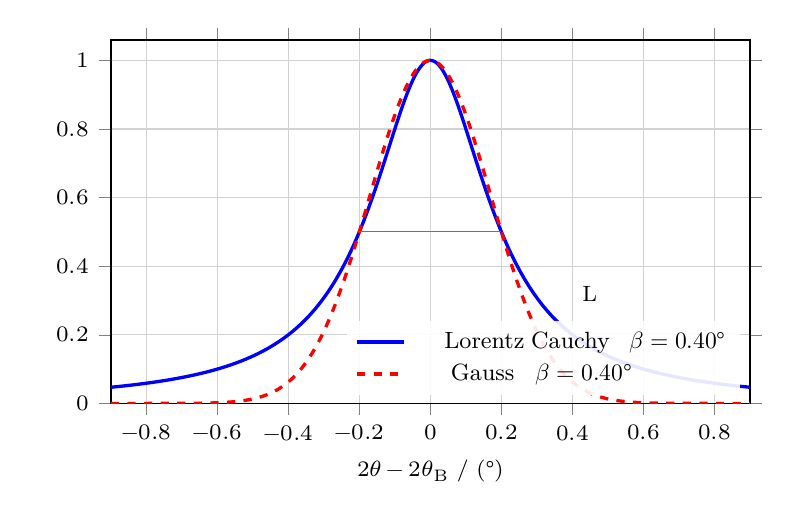
\begin{tikzpicture}
    \tikzset{declare function={
        Lz(\x) = 1/(1+25*\x*\x);
        Gz(\x) = exp(-17.3286*\x*\x);
      }}
    \begin{axis}[
        width=\onecolwidth, height=62mm,
        xlabel={$2\theta-2\theta_{\mathrm{B}}$ / (°)},
        ylabel={归一化强度},
        xmin=-0.9, xmax=0.9, ymin=0, ymax=1.06,
        xtick={-0.8,-0.6,-0.4,-0.2,0,0.2,0.4,0.6,0.8},
        ytick={0,0.2,0.4,0.6,0.8,1.0},
        grid=both, major grid style={gray!35}, minor grid style={gray!12},
        tick label style={font={\fontsize{8}{9.6}\selectfont}},
        label style={font={\fontsize{8}{9.6}\selectfont}},
        legend style={font={\fontsize{8}{9.6}\selectfont}, draw=none,
                      fill=white, fill opacity=0.9, text opacity=1,
                      legend cell align=left,
                      at={(0.985,0.02)}, anchor=south east},
        samples=401, domain=-0.9:0.9,
      ]
      \addplot[very thick, blue] {Lz(x)};
      \addlegendentry{尺寸宽化：Lorentz（Cauchy）型，$\beta=0.40°$}
      \addplot[very thick, red, dashed] {Gz(x)};
      \addlegendentry{微应变宽化：Gauss 型，$\beta=0.40°$}
      \addplot[black!55, thin, sharp plot, update limits=false]
        coordinates {(-0.2,0.5) (0.2,0.5)};
      \node[anchor=west, font={\fontsize{8}{9.6}\selectfont}]
        at (axis cs:0.40,0.32) {L 型尾部明显更重};
    \end{axis}
  \end{tikzpicture}
  \caption{同一半峰宽下两种宽化机制的峰形差别（模型计算）。\textbf{看什么}：两条曲线的半峰宽
    完全相同（都取 $\beta=0.40°$，横线标出半高位置），但\textbf{尾部}完全不同——在
    $\pm1.5\beta$（即 $\pm0.6°$）处 Lorentz 型还剩约 $10\%$ 的强度，Gauss 型只剩约 $0.2\%$。
    \textbf{条件与用法}：晶粒尺寸引起的宽化接近 Lorentz（Cauchy）型，微应变引起的宽化接近
    Gauss 型；因此\textbf{峰尾形状是判断宽化来源的第一条线索}，也是``用半峰宽一个数反推一个
    原因''会出错的原因。\textbf{局限}：这是理想化的单峰，实际谱线是仪器函数与样品函数的卷积，
    仪器函数的尾部也会抬高峰尾，必须先扣除仪器贡献才能用尾部形状作判断。
    \figsrc{模型计算图，非原书插图。}\modelmark}
  \label{fig:ch04c-profile}
\end{figure}

\begin{example}[读图实例：同一个半峰宽，可能对应完全不同的样品]
\begin{obs}
图~\figref{fig:ch04c-profile} 中两条曲线：（a）实线，Lorentz 型，$\beta=0.40°$；
（b）虚线，Gauss 型，$\beta=0.40°$。在 $2\theta-2\theta_{\mathrm{B}}=\pm0.2°$ 处两线重合于
$0.5$；在 $\pm0.4°$ 处实线约 $0.20$、虚线约 $0.06$；在 $\pm0.6°$ 处实线约 $0.10$、虚线约
$0.002$；在 $\pm0.8°$ 处实线仍有约 $0.06$，虚线已低于 $10^{-4}$。
\end{obs}
\begin{infer}
两条曲线在\textbf{半高宽这一个数上没有任何区别}，差别全部在尾部。因此：
（1）仅凭半峰宽无法区分``小晶粒''与``大晶粒加微应变''，二者可以给出同一个 $\beta$；
（2）实测峰尾明显厚重、且用 Lorentz 型拟合远好于 Gauss 型时，宽化更可能来自尺寸；
峰尾衰减很快、Gauss 型拟合更好时，更可能来自应变分布；
（3）对重叠峰定量、对弱峰判识（例如杂质相的最强线与主相峰尾重叠）时，峰形函数选错会带来
系统性误差，而不是随机误差。这条判断不是定论性判据，必须用多条不同角度的峰联合检验
（见后文 Williamson--Hall 图）。
\end{infer}
\end{example}

\begin{table}[tbp]
  \centering
  \caption{Scherrer 方程给出的半峰宽与晶粒尺寸的对应（按式~\equref{eq:ch04c-scherrer} 计算，
    $K=0.89$，Cu $K\alpha_{1}$ 即 $\lambda=1.5406$ Å，取 $2\theta=30°$）。\textbf{读法}：
    尺寸大于约 $100$ nm 时，尺寸宽化已降到 $0.1°$ 以下，与仪器宽化同量级甚至更小，
    \textbf{再谈''用半峰宽算尺寸''已无意义}；尺寸小于约 $2$ nm 时半峰宽达 $4°$ 以上，
    峰与背景难以分开，读数误差迅速放大。最后一列给出按 $0.02°$ 步长扫描时一个半峰宽内的
    采样点数，点数少于约 $5$ 时峰形已不可靠。\src{本表为本改编本归纳，非源书表格；依据上册 §4.7，
    书内 p.270—278 / PDF p.289—297。表中数值为本改编本按 Scherrer 方程计算的模型值，非源书实验数据。}}
  \label{tab:ch04c-scherrer}
  \begin{tabular}{@{}rrr@{}}
    \toprule
    $D_{hkl}$ / nm & $\beta(2\theta)$ / (°) & 每 $0.02°$ 的采样点数 \\
    \midrule
    100 & 0.081 & 4 \\
    50  & 0.163 & 8 \\
    20  & 0.407 & 20 \\
    10  & 0.813 & 41 \\
    5   & 1.63  & 81 \\
    2   & 4.07  & 204 \\
    \bottomrule
  \end{tabular}
\end{table}

\begin{dataflow}
\textbf{从一张峰到一个小数}：
实测峰（步进扫描数据）$\rightarrow$ 扣背景 $\rightarrow$ 剥离 $K\alpha_{2}$（若双线分离）
$\rightarrow$ 峰形函数拟合得总半峰宽 $B$ $\rightarrow$ 由标样或基本参数法得仪器宽化 $b$
$\rightarrow$ 解卷积得样品宽化 $\beta$ $\rightarrow$ 由式~\equref{eq:ch04c-scherrer} 得
$D_{hkl}$ $\rightarrow$ 用多条不同角度的峰检验 $\beta\cos\theta$ 是否随 $\sin\theta$ 变化
（判断是否含微应变）。任何一步没做，后面得到的数都不叫``晶粒大小''。
\end{dataflow}

\subsubsection{衍射峰分析与 Scherrer 方程的应用}

实验得到的半峰宽 $B$ 是仪器因子与样品因子\textbf{共同}作用的结果，即衍射图谱可以看成仪器
函数与样品函数的\textbf{卷积}（convolution）：用一个函数去``调制展开''另一个函数。第一步
就是分离仪器因素。

\paragraph{仪器因素的处理}
\begin{principle}
设仪器函数为 $g(x)$、样品函数为 $f(x)$，实测峰形为二者的卷积
\begin{equation}
h(x)=\int g(x')\,f(x-x')\,\mathrm{d}x' .
\label{eq:ch04c-conv}
\end{equation}
卷积没有简单的``减法''，但在两种极限峰形下有可用的近似：
\begin{equation}
\text{Gauss 型：}\ B^{2}=b^{2}+\beta^{2}\ \Rightarrow\ \beta=\sqrt{B^{2}-b^{2}};
\qquad
\text{Lorentz 型：}\ B=b+\beta\ \Rightarrow\ \beta=B-b .
\label{eq:ch04c-subtract}
\end{equation}
真实峰形介于两者之间，两端近似都不成立，此时应使用\textbf{工作曲线}（用已知函数把仪器函数
与模型样品函数卷积，得到 $B$ 与 $\beta$ 的对应关系，见本节 ZnO 实例中的原书图 4-28）或直接
做全谱拟合。获取仪器函数 $b(\theta)$ 有两条路：\\
（1）\textbf{标样法}：选结晶良好、晶粒远大于 $100$ nm 且无应变的标样（原书用晶粒约
$10$ µm 的 $\alpha$-石英），在待测峰附近测一条衍射，其宽度即为该角度下的仪器宽化。
必须注意 $b$ 随角度变化，用低角测得的 $b$ 去修高角峰会带来系统误差。\\
（2）\textbf{基本参数法}：由仪器几何（狭缝宽度、靶斑尺寸、样品透明度、轴向发散等）直接
计算仪器函数，不需要标样，适合样品量少或找不到合适标样的情况。\\
随着仪器改进，现代衍射仪的仪器贡献半峰宽一般可以控制在 $0.05°$ 甚至更小。因此当晶粒不是
很大（宽化明显）时，忽略仪器因素或简单相减尚可接受；但\textbf{当算出的尺寸进入几十纳米
以上时，仪器宽化就必须扣除}——它已是分母中的主要项。
\end{principle}

\paragraph{$K\alpha_{1}$ 与 $K\alpha_{2}$ 的双线加和与分离}
\begin{principle}
衍射实验通常用 $K\alpha$ 辐射，它由 $K\alpha_{1}$ 与 $K\alpha_{2}$ 两条线组成，强度比近似为
$2:1$。二者峰形类似而波长不同，产生的衍射峰错开一个 $\Delta(2\theta)$，线性叠加后给出实验
谱（原书图 4-20）。由布拉格方程 $2d\sin\theta_{1}=n\lambda_{1}$、$2d\sin\theta_{2}=n\lambda_{2}$，
$\Delta(2\theta)=2(\theta_{2}-\theta_{1})$，利用三角变换并作小量近似（$\sin\theta$ 的微分）得
\begin{equation}
\Delta(2\theta)=\frac{2\Delta\lambda}{\lambda}\,\mathrm{tg}\,\theta .
\label{eq:ch04c-doublet}
\end{equation}
对铜靶，$\lambda_{1}=1.5406$ Å、$\lambda_{2}=1.5444$ Å，$\Delta\lambda=0.0038$ Å，
$K\alpha$ 加权平均值 $\bar{\lambda}=1.5418$ Å；代入得双线分离度
\tocheck{未对照原页面图像：原书此处给出 $\Delta(2\theta)=0.2246\,\mathrm{tg}\,\theta$。
按式~\equref{eq:ch04c-doublet} 用铜靶数值复算应为 $2\times0.0038/1.5418=4.93\times10^{-3}$
弧度 $=0.282°$，即 $0.282\,\mathrm{tg}\,\theta$（以度为单位）；两者相差约 $20\%$，
$\lambda$、$\Delta\lambda$ 的取值口径（是否用加权平均、是否以 pm 计）原书未在此处写明，
数字待核。}
\begin{equation}
\Delta(2\theta)\big/°\approx0.28\,\mathrm{tg}\,\theta .
\label{eq:ch04c-doubletnum}
\end{equation}
波长短的靶（Mo）双线分离更严重；同一靶下低角度分离度小、高角度分离越来越明显（原书
图 4-21 给出铜靶、铝靶、铁靶的 $\Delta(2\theta)$—$2\theta$ 曲线，可据图直接查出各角度的
分离度）。
\end{principle}

\begin{measure}
\textbf{双线分离的 Rachinger 法}。由于两条线的叠加是线性加合，可以按 $\Delta(2\theta)/n$
的等间隔把峰划分为若干区间。取 $n=3$（即以 $\Delta(2\theta)/3$ 为间隔读数），第 $i$ 点上的
$K\alpha_{2}$ 贡献等于第 $i-3$ 点上 $K\alpha_{1}$ 贡献的一半，于是有递推
\begin{equation}
I_{i}(\alpha_{1})=I_{i}-\tfrac{1}{2}I_{i-3}(\alpha_{1}),
\qquad i=4,5,6,\dots
\label{eq:ch04c-rachinger}
\end{equation}
从第 1 区到第 3 区没有 $K\alpha_{2}$ 贡献，可以直接取 $I_{1},I_{2},I_{3}$ 作为
$I(\alpha_{1})$ 的起点，然后逐点向右递推，得到纯 $K\alpha_{1}$ 的强度曲线。\\
\textbf{适用边界（原书明确指出）}：从起始角到峰最大值之后约一半的位置，递推结果较好；再往后，
$I_{i}(\alpha_{1})$ 与 $\tfrac{1}{2}I_{i-3}(\alpha_{1})$ 已接近，两者相减的误差被放大，曲线
出现起伏，\textbf{分离出的 $\alpha_{1}$ 曲线在后半段准确性较差}。另有一个更基本的前提：
式~\equref{eq:ch04c-rachinger} 只在该角度上双线确实分离（$\Delta(2\theta)$ 与半峰宽可比或更大）
时才有意义；纳米样品低角峰宽化严重、双线根本不分离，此时强行剥离只会制造假的起伏。
\end{measure}

\begin{pitfall}
\textbf{不扣仪器宽化，得到的尺寸系统偏小。}这是本节最常见、也最容易被忽略的错误，因为它
不产生任何异常现象。定量地看：若仪器宽化 $b$ 与样品宽化 $\beta$ 大致相当，而直接用实测 $B$
代入 Scherrer 公式，则得到的 $D'$ 满足
\begin{equation}
D'=\frac{K\lambda}{B\cos\theta}\approx\frac{K\lambda}{2\beta\cos\theta}=\frac{D}{2}
\qquad(\text{Lorentz 型极限},\ B=b+\beta,\ b\approx\beta),
\label{eq:ch04c-halving}
\end{equation}
即\textbf{尺寸被算小约一半}。概括地说：（i）$B$ 是仪器与样品卷积的结果，直接代入等于把仪器
的``宽''记在晶粒的账上；（ii）宽化越弱（晶粒越大）这个错误越严重——尺寸大于 $100$ nm 时，
实测宽度几乎全是仪器贡献，此时算出的``尺寸''实际是仪器分辨率决定的假值；（iii）仪器宽化
随角度变化，用一个固定值去扣整张谱同样会残留系统误差。判别方法：换一台分辨率更高的仪器
或改用更小的狭缝重测，若``尺寸''随之改变，说明之前的数主要是仪器贡献。
\end{pitfall}

\paragraph{尺寸宽化与微应变宽化的分离：Williamson--Hall 图}
\begin{principle}
晶粒变小往往同时伴随晶格畸变，实际峰形是两种效应的叠加。微应变 $\varepsilon=\Delta d/d$ 使
不同晶粒、不同晶面的 $d$ 值在一个范围内分布，峰位随之弥散，宽化量随 $\mathrm{tg}\,\theta$
增大；尺寸宽化则按 $1/\cos\theta$ 变化。把 Scherrer 公式与应变的贡献写成一项加和
\begin{equation}
\beta_{hkl}=\frac{K\lambda}{D\cos\theta}+4\varepsilon\,\mathrm{tg}\,\theta
\quad\Longleftrightarrow\quad
\beta_{hkl}\cos\theta=\frac{K\lambda}{D}+4\varepsilon\sin\theta ,
\label{eq:ch04c-WH}
\end{equation}
两边同乘 $\cos\theta$ 后，$\beta\cos\theta$ 对 $4\sin\theta$ 作图应是一条直线：\textbf{截距}
给出尺寸（$D=K\lambda/\text{截距}$），\textbf{斜率}给出微应变（$\varepsilon=\text{斜率}$）。
这就是 Williamson--Hall（WH）图。若各点不能用一条直线拟合，说明尺寸分布过宽、应变各向异性
或存在择优取向，此时应改用更完整的全谱模型（如 Rietveld 中的各向异性宽化模型）而不是硬划
直线。\tocheck{未对照原页面图像：原书 §4.7 未给出 Williamson--Hall 关系式，本段是按标准
文献形式补充的，用于说明 Scherrer 公式与应变宽化的分工；式~\equref{eq:ch04c-WH} 中
晶体学惯例的 $4\varepsilon\sin\theta$ 系数（有的文献写作 $2\varepsilon\sin\theta$）取决于
$\varepsilon$ 与积分宽度的定义，引用时须与本处定义一致。}
\end{principle}

\begin{figure}[tbp]
  \centering
  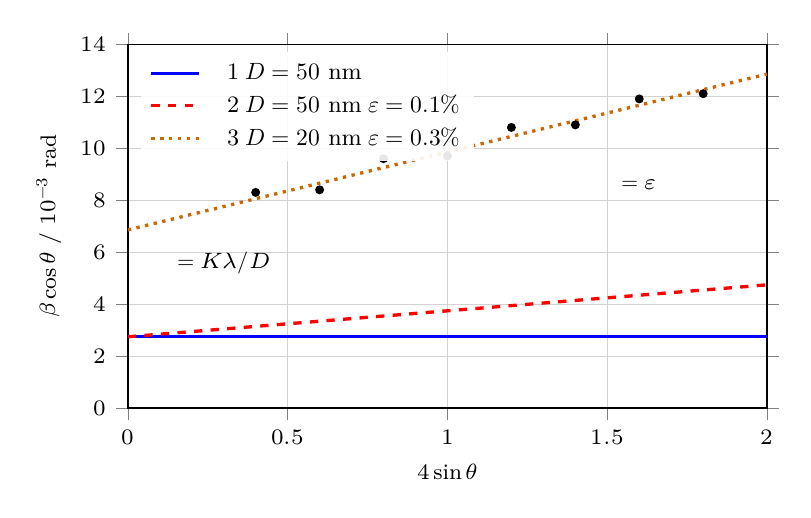
\begin{tikzpicture}
    \tikzset{declare function={
        WHa(\x) = 2.742;
        WHb(\x) = 2.742+1.0*\x;
        WHc(\x) = 6.856+3.0*\x;
      }}
    \begin{axis}[
        width=\onecolwidth, height=62mm,
        xlabel={$4\sin\theta$},
        ylabel={$\beta\cos\theta$ / $10^{-3}$ rad},
        xmin=0, xmax=2.0, ymin=0, ymax=14,
        xtick={0,0.5,1.0,1.5,2.0},
        ytick={0,2,4,6,8,10,12,14},
        grid=both, major grid style={gray!35}, minor grid style={gray!12},
        tick label style={font={\fontsize{8}{9.6}\selectfont}},
        label style={font={\fontsize{8}{9.6}\selectfont}},
        legend style={font={\fontsize{8}{9.6}\selectfont}, draw=none,
                      fill=white, fill opacity=0.9, text opacity=1,
                      legend cell align=left,
                      at={(0.02,0.98)}, anchor=north west},
        samples=2, domain=0:2,
      ]
      \addplot[very thick, blue] {WHa(x)};
      \addlegendentry{样品 1：$D=50$ nm，无微应变}
      \addplot[very thick, red, dashed] {WHb(x)};
      \addlegendentry{样品 2：$D=50$ nm，$\varepsilon=0.1\%$}
      \addplot[very thick, orange!80!black, dotted] {WHc(x)};
      \addlegendentry{样品 3：$D=20$ nm，$\varepsilon=0.3\%$}
      \addplot[only marks, mark=*, mark size=1.3pt, black] coordinates {
        (0.4,8.3) (0.6,8.4) (0.8,9.6) (1.0,9.7) (1.2,10.8) (1.4,10.9) (1.6,11.9) (1.8,12.1)
      };
      \node[anchor=west, font={\fontsize{8}{9.6}\selectfont}]
        at (axis cs:0.06,5.6) {截距 $=K\lambda/D$};
      \node[anchor=west, font={\fontsize{8}{9.6}\selectfont}]
        at (axis cs:1.45,8.6) {斜率 $=\varepsilon$};
    \end{axis}
  \end{tikzpicture}
  \caption{用 Williamson--Hall 图分离尺寸与微应变（模型计算，按式~\equref{eq:ch04c-WH}，
    $K=0.89$，$\lambda=1.5406$ Å）。\textbf{看什么}：三个样品的横轴量都是
    $4\sin\theta$、纵轴量都是 $\beta\cos\theta$。（i）样品 1 只有尺寸贡献，是一条水平线，
    高度即 $K\lambda/D$；（ii）样品 2 的晶粒与样品 1 相同而多了 $0.1\%$ 的微应变，截距不变、
    斜率变正——\textbf{尺寸只由截距决定，与斜率无关}；（iii）样品 3 晶粒更小，三条线里截距
    最大。黑点为样品 3 的模拟实测点（带约 $\pm3\%$ 的随机误差），可见两三个角度的数据不足以
    定直线。\textbf{条件与局限}：要求各峰宽化只来自尺寸与均匀微应变，且无择优取向；若峰形
    偏离、存在层错或成分不均匀，点会系统偏离直线，此时 WH 图的作用是\textbf{提示模型不足}，
    而不是给出可用的 $D$ 和 $\varepsilon$。\figsrc{模型计算图，非原书插图。}\modelmark}
  \label{fig:ch04c-WH}
\end{figure}

\begin{table}[tbp]
  \centering
  \caption{Scherrer 方程适用的条件与典型失效方式。左列是使用者的操作，右列是后果。凡是
    右列的现象出现，都应先回到左列检查，而不是修改结论。\src{据上册 §4.7，
    书内 p.270—278 / PDF p.289—297 归纳。}}
  \label{tab:ch04c-boundary}
  \begin{tabular}{@{}p{46mm}p{100mm}@{}}
    \toprule
    操作或前提 & 后果与判别 \\
    \midrule
    用未扣仪器宽化的 $B$ 直接代入 & 尺寸系统偏小，晶粒越大偏得越多（式~\equref{eq:ch04c-halving}）；
    换仪器或换狭缝重测，结果会变 \\
    存在微应变而只做 Scherrer & 把应变宽化记在尺寸上，算出``尺寸''显著小于 TEM 观察值；
    用 WH 图看 $\beta\cos\theta$ 是否随 $\sin\theta$ 上升即可识别 \\
    存在宽尺寸分布 & Scherrer 给出的是体积加权平均值，与 TEM 数均粒径、比表面等效粒径
    可以差出数倍，三者不可直接互比 \\
    峰太宽或太窄 & 尺寸大于约 $100$ nm 或小于约 $2$ nm 时，公式仍在，但读数与背景分离的
    误差已超过结论本身的分辨能力 \\
    用峰顶高度代替半峰宽 & 峰高受取向、织构、重叠影响，与半峰宽不是同一个量，量纲上也不
    构成宽度 \\
    \bottomrule
  \end{tabular}
\end{table}

\begin{pitfall}
\textbf{Scherrer 结果的四种典型误判}，都可先用一条内部判据自查：\\
（1）\textbf{算出负尺寸或荒谬小的尺寸}。式~\equref{eq:ch04c-subtract} 的 $\beta=\sqrt{B^{2}-b^{2}}$
在 $b>B$ 时无解；用 Lorentz 型相减时 $\beta=B-b$ 可能为负。这不是样品``负晶粒''，而是
\textbf{仪器宽化被高估或标样选错}（标样本身有宽化、或不在同一角度）。正确处理：换标样、
改用工作曲线或基本参数法。\\
（2）\textbf{得到的尺寸远小于 TEM 观察值}。常见三种原因：未扣仪器宽化（式~\equref{eq:ch04c-halving}，
因子约 $2$）；把微应变当成尺寸（应变可轻松贡献 $0.1°$—$0.5°$，等价于把尺寸压到几纳米）；
样品本身是多晶团聚体，TEM 量的是颗粒而衍射量的是相干散射柱长。三者可用``换仪器''、
``WH 图''、``不同 $hkl$ 的 $D$ 是否一致''分别排除。\\
（3）\textbf{把微应变当尺寸}。判据是 $D_{hkl}$ 随 $hkl$ 系统变化——尺寸效应下不同方向的
$D_{hkl}$ 差异有晶体学含义（各向异性形貌），而应变效应表现为所有峰的宽度都随
$\mathrm{tg}\,\theta$ 增长。只看一条峰无法区分。\\
（4）\textbf{只报一个数}。任何 Scherrer 结果都应同时给出：所用 $K$、波长、$2\theta$ 范围、
仪器宽化的来源与数值、是否剥离 $K\alpha_{2}$。缺任一项，这个数无法被复核。
\end{pitfall}

\begin{crosscheck}
Scherrer 结果必须与独立方法互校，且\textbf{不同方法量的是不同的平均}，一致时才说明样品
简单，不一致时往往能反过来提供信息：\\
（1）\textbf{TEM/HRTEM}：给出数均粒径与形貌。衍射值与 TEM 值一致 $\Rightarrow$ 单尺寸分布、
无应变；衍射值小于 TEM $\Rightarrow$ 存在应变或多晶团聚；不同 $hkl$ 的 $D_{hkl}$ 与 TEM
形貌（片状、针状）应对应得上。\\
（2）\textbf{物理吸附／比表面}：由 $S_{\mathrm{BET}}$ 换算等效粒径
$d\approx6/(\rho S)$，可与体积平均尺寸比较；此法给出的是外表面积等效尺寸，与相干长度同量级
但不相等。\\
（3）\textbf{小角散射（SAXS）}：给出颗粒尺寸分布，可判断``单尺寸''这一前提是否成立。\\
（4）\textbf{中子衍射与 PDF}：中子对轻原子敏感且峰形更接近 Gauss，可分辨尺寸与应变；
PDF 直接给出短程结构，不受晶粒尺寸限制。\\
（5）\textbf{全谱拟合（Rietveld）}：把尺寸与应变作为峰宽参数一起精修，是当前最通用的做法，
但它与 Scherrer 一样依赖峰形模型，不能作为完全独立的校验。
\end{crosscheck}

\subsection{Rietveld 全谱拟合}
\src{上册 §4.8，书内 p.278—284 / PDF p.297—303}

晶体结构解析通常由单晶衍射数据确定，但许多化合物难以长出单晶，有些材料的性质本身就体现在
多晶状态，因此用多晶衍射数据做结构分析是必须进行的工作。早期的多晶结构分析靠提取积分强度，
再用类似单晶的方法处理；由于粉末衍射峰严重重叠、强度难以合理分配，可用的有效数据很少，只能
做较简单的结构且准确度差。20 世纪 60 年代 Rietveld 提出``全图拟合''方法，使基于多晶数据的
结构精修成为结构分析的重要方法之一；峰形拟合物相分析与晶胞参数修正、晶体结构精修、无标相
定量、结构从头解析等，Rietveld 方法已深入到多晶衍射分析的各个方面。

\begin{probout}
\textbf{测什么}：整张步进扫描谱（每一个 $2\theta$ 数据点都是一个观测点），而不是一张峰表。\\
\textbf{能推断什么}：晶胞参数（可达 $10^{-4}$—$10^{-5}$ 相对精度）、原子坐标、占位度、
温度因子、各相含量、晶粒尺寸与微应变、择优取向参数——前提是有合理的初始结构模型。\\
\textbf{不能推断什么}：Rietveld 是\textbf{精修}方法而非求解方法，它不会从一个错误的模型出发
找到正确答案；轻原子（H、Li、O）在 X 射线数据中约束很弱；强相关的参数组合（占位度与温度
因子、晶胞参数与零点）不能由同一套数据独立确定；拟合优度高也\textbf{不等于}结构模型正确。
\end{probout}

\subsubsection{Rietveld 方法的基本原理}

\begin{principle}
Rietveld 方法处理多晶数据时不再分离衍射峰，而是反其道而行：把由初始模型计算出的强度分解，
与各实验点数据关联。其基本要点为：\\
（1）\textbf{采用步进扫描的实验数据}，每个数据点都是观测点；\\
（2）\textbf{设置初始结构模型}，为拟分析的物相找到或建立较合理的初始结构；\\
（3）\textbf{峰形函数拟合}，用合适的数学函数模拟衍射峰，把初始模型算出的积分强度分解成与
各步对应的计算值；\\
（4）\textbf{最小二乘全图拟合}，逐点比较计算值与实验值，修正结构参数，得到与实验数据对应的
晶体结构参数。\\
由初始结构模型计算出的衍射强度是某一衍射指标的积分强度（与 §4.4 给出的积分强度表达式同源，
只是把几何与物理因子统一归入比例因子与修正项）
\begin{equation}
I_{hkl}=K\cdot P\cdot L\cdot\left|F_{hkl}\right|^{2}\cdot D\cdot A ,
\label{eq:ch04c-ihkl}
\end{equation}
确定峰形函数后，把它展开成按 $2\theta$ 分布的强度。第 $i$ 个角度处的计算强度为
\begin{equation}
Y_{ic}=Y_{ib}+\sum_{\varphi}S_{\varphi}\sum_{\{hkl\}_{\varphi}}
j_{hkl}\,L_{hkl}\left|F_{hkl,\varphi}\right|^{2}\Omega\!\left(2\theta_{i}-2\theta_{hkl,\varphi}\right),
\label{eq:ch04c-rietveld}
\end{equation}
式中 $Y_{ib}$ 为该角度的背景值，$S_{\varphi}$ 为第 $\varphi$ 相的比例因子，$j_{hkl}$ 为多重性
因子，$L_{hkl}$ 为洛伦兹--偏振因子，$\Omega$ 为归一化的峰形函数（其半峰宽随角度变化），
对 $\varphi$ 加和表示对所有物相加和，对 $hkl$ 加和表示对所有衍射指标加和。背景可用多项式
拟合求得，也可读入背景值后作内插。
\tocheck{未对照原页面图像：式~\equref{eq:ch04c-rietveld} 的原书排版ocr严重残缺（下标、
加和号与括号位置不可辨）。本式按标准 Rietveld 公式重建；原书明确给出的只有：$S$ 为比例
因子、$2\theta_{hkl}$ 为布拉格角、$I_{hkl}$ 为某相某指标的积分强度、$P$ 为峰形函数、
$Y_{ib}(2\theta_{i})$ 为背景值。式~\equref{eq:ch04c-ihkl} 中的因子顺序同样存疑。}
\end{principle}

\begin{measure}
\textbf{衍射数据收集：Rietveld 结果的精度上限由数据决定。}\\
（1）\textbf{样品}：结晶良好、晶粒大小适宜（研磨至 $10$\,µm 以下以减小消光与微吸收），
尽可能消除择优取向。Bragg--Brentano 几何宜选较大的样品架并让样品转动，Debye--Scherrer
几何可选毛细管装样，以保证有大量晶粒参与衍射。\\
（2）\textbf{角度范围}：$2\theta$ 起始角从第一个峰之前 $2°$—$3°$ 开始，终止角到
$120°$—$130°$（高角数据对晶胞参数与温度因子最重要，不应为了省时间砍掉）。\\
（3）\textbf{步长与计数}：步长常取 $0.01°$—$0.02°$，每步数秒到数十秒（按仪器功率与探测器
效率定）。选择计数时间的原则是使\textbf{最强衍射峰最高处的计数约为两万}。计数时间长，强度高、
信噪比好、统计误差小、弱峰明确；但强到一定程度后改善有限，\textbf{甚至可能引入另外的
``误差''导致拟合优度变差}——这一点在下面结合 $R$ 因子讨论，是理解 $R$ 因子的关键。
\tocheck{未对照原页面图像：原书此处步长作``0.01—''后截断，''步长选 0.01—0.02°''为按
上下文与常规取值补全；终止角原书作 1200—1300，按上下文应读作 120°—130°。}
\end{measure}

\begin{dataflow}
\textbf{一次 Rietveld 精修的标准流程}：
（i）收集步进扫描数据 $\rightarrow$（ii）确定背景与峰形函数，做\textbf{峰形拟合}
（Pawley 或 LeBail，见 §4.8.2），得到晶胞参数、零点、峰宽参数与峰位 $\rightarrow$
（iii）代入结构模型，先只精修比例因子与背景 $\rightarrow$（iv）逐步放开晶胞参数、零点、
峰宽、取向，最后放开原子坐标、占位度、温度因子 $\rightarrow$（v）检查拟合差谱是否还有
系统性残差（残差有结构 $\Rightarrow$ 模型或峰形有问题；残差随机 $\Rightarrow$ 拟合已到底）
$\rightarrow$（vi）检查结构参数的物理合理性（键长键角、占位度总和、温度因子非负且量级
合理）$\rightarrow$（vii）报告结果时必须同时给出 $R_{\mathrm{wp}}$、$R_{p}$、$R_{\mathrm{exp}}$、
拟合差谱与参数的标准偏差。
\end{dataflow}

\subsubsection{峰形函数与最小二乘全图拟合}

\begin{principle}
峰形函数的选择非常重要，表~\tabref{tab:ch04c-profile} 列出常用的几类。对某衍射峰，取布拉格
角处的 $2\theta=0$ 向两边展开：Gauss 函数图形变化较缓、拖尾效应小；Lorentz（Cauchy）函数
图形变化较快、拖尾效应大（原书图 4-24 即两个函数的对比）。对于粉末中子衍射，峰形接近 Gauss
函数；对于 X 射线衍射，实际峰形介于二者之间，是 Gauss 与 Lorentz 函数的``组合''，按权重加和
即 pseudo-Voigt 函数。峰形与仪器、样品特征都有关，得到数据后必须通过对实验数据的拟合确定
函数类型与参数，而不是先验指定。
\end{principle}

\begin{table}[tbp]
  \centering
  \caption{多晶衍射图拟合常用的峰形函数（对应原书表 4-8）。第三列为半峰宽随衍射角变化的
    参数化，$U,V,W$ 与 $X,Y,F$ 都是拟合参数。\textbf{选择判据}：以拟合差谱的残差是否有
    结构为准，不以单个 $R$ 因子最小为准。\src{据上册 §4.8 与表 4-8，
    书内 p.278—284 / PDF p.297—303 整理。}}
  \label{tab:ch04c-profile}
  \begin{tabular}{@{}lll@{}}
    \toprule
    函数类型 & 表达式（示意） & 半峰宽 $\Gamma$ 的参数化 \\
    \midrule
    Gaussian & $G(x)=\dfrac{1}{\sigma\sqrt{2\pi}}\exp\!\left(-\dfrac{x^{2}}{2\sigma^{2}}\right)$
      & $\Gamma^{2}=U\mathrm{tg}^{2}\theta+V\mathrm{tg}\,\theta+W$ \\
    Lorentzian & $L(x)=\dfrac{\Gamma/2}{\pi\left(x^{2}+\Gamma^{2}/4\right)}$
      & $\Gamma=X\mathrm{tg}\,\theta+(Y+F)/\cos\theta$ \\
    Voigt & $q(x)=G(x)*L(x)$（卷积） & —— \\
    pseudo-Voigt & $q(x)=\eta L(x)+(1-\eta)G(x)$ & $\eta$ 为 Lorentz 成分的权重 \\
    \bottomrule
  \end{tabular}
\end{table}

\begin{pitfall}
\textbf{表~\tabref{tab:ch04c-profile} 与 $\Gamma$ 参数化的使用边界}：\\
（1）$\Gamma^{2}=U\mathrm{tg}^{2}\theta+V\mathrm{tg}\,\theta+W$ 是 Caglioti 型参数化，它把半峰宽
写成角度的光滑函数，因此\textbf{隐含``所有峰的宽化机制相同''}；当样品同时有尺寸宽化与各向
异性应变时，只用这一组参数拟合会把二者混在一起。\\
（2）pseudo-Voigt 的 $\eta$ 与 $\Gamma$ 之间有强相关：$\Gamma$ 变大与 $\eta$ 变小在一定范围内
可以给出几乎相同的曲线，因此单独报告 $\eta$ 或 $\Gamma$ 的物理含义有限。\\
（3）原书中 modified Lorentzian 的表达式与半峰宽参数化在本页 ocr 中不可辨，本表未列出，
以免给出错误的公式形式。\tocheck{未对照原页面图像：modified Lorentzian 的函数式与
$\Gamma$ 参数化未能从 ocr 重建；Lorentzian 一行中 $(Y+F)/\cos\theta$ 的括号内容（原书此处
似为两项之和）亦存疑。}
\end{pitfall}

\subsubsection{峰形拟合：Pawley 方法与 LeBail 方法}

\begin{principle}
要从多晶数据中解析结构，必须提取不同衍射指标的强度，于是又回到多晶衍射峰的重叠问题。随着
高速计算机与高分辨衍射仪的使用，\textbf{全图分解}（whole powder pattern decomposition）成为
解决这一问题的重要方法：采用``分解''拟合而不是去卷积来处理多晶衍射图。常用两种方法：\\
（1）\textbf{Pawley 方法}（1980）：不考虑结构因子，直接从实验数据出发拟合衍射图。随角度
变化的衍射图由以下参数确定——每个指标 $hkl$ 的强度 $I_{hkl}$（$N$ 个指标即 $N$ 个强度参数）、
晶胞参数 $a,b,c,\alpha,\beta,\gamma$（6 个）、仪器零点修正（1 个）、峰宽参数 $U,V,W$（3 个）、
以及与峰形函数选取有关的其他参数（$m$ 个，如 Lorentz 与 Gauss 成分的权重）。拟合参数总数
为 $N+10+m$。对分离度好的峰，峰强由实验强度确定；对重叠严重的峰（尤其两峰位之差
$\Delta2\theta$ 小于数据步长时）需\textbf{硬性限定}：按各指标衍射强度相等分配实验强度；
若严重重叠但尚可分开，则采用\textbf{软性约束}：从强度均匀分配出发进行修正。\\
（2）\textbf{LeBail 方法}（1988）：仍用上述 $10+m$ 个参数做最小二乘拟合，但强度不纳入拟合，
而用``赋值—计算—赋值''的循环确定：先给各衍射峰一个大致的初值作为``计算值''，用 Rietveld
拟合程序按所赋计算值对实验观察值进行分配，算出的观察值再设为新的计算值，对 $10+m$ 个参数
做最小二乘修正，循环直到收敛。此法又称衍射强度分配法，\textbf{对任意数目的重叠峰都适用}；
由于每步参与最小二乘的只有晶胞参数与峰形参数，各步运行很快，总时间大大缩短。注意：由于
拟合中把实验值赋作计算值，原则上 $R$ 因子应趋于 $0$——这一点正是下面正确理解 $R$ 因子的
关键。
\end{principle}

\begin{table}[tbp]
  \centering
  \caption{Pawley 方法与 LeBail 方法的对照。两者都只拟合``非结构''参数，因此它们是
    Rietveld 精修的\textbf{前置步骤}，其 $R$ 因子构成结构精修 $R$ 因子的下界。\src{据上册 §4.8，
    书内 p.278—284 / PDF p.297—303 归纳。}}
  \label{tab:ch04c-fitmethods}
  \begin{tabular}{@{}p{24mm}p{56mm}p{62mm}@{}}
    \toprule
    比较项 & Pawley 方法 & LeBail 方法 \\
    \midrule
    拟合参数 & $N+10+m$（含每个 $hkl$ 的强度） & $10+m$（强度不参与拟合） \\
    强度来源 & 最小二乘直接给出，并给出误差 & 赋值—计算—赋值循环，迭代收敛 \\
    收敛速度 & 参数多、计算量大，较慢 & 每步参数少，运行快，但迭代步数多 \\
    适用性 & 重叠峰的强度分配可能不尽合理 & 对任意重叠数目都适用 \\
    $R$ 因子的意义 & 反映强度分配的好坏 & 原则上趋于 $0$，不能与结构精修的 $R$ 相比 \\
    \bottomrule
  \end{tabular}
\end{table}

\begin{dataflow}
\textbf{峰形拟合的实际用处}（原书列出四点，都超出``只为提取强度''）：
（i）在没有合适结构模型、或只需要准确晶胞参数时，可快速处理衍射图并得到相关信息；
（ii）有助于判断空间群设定是否合理——例如 $Pnma$ 与 $Pbma$ 很难从强度上看出哪个更合理，
峰形拟合可以较快给出选择；（iii）给出计算值与实验值的直观比较，直接显示体系是单一物相还是
含有杂相；（iv）由于计算强度与结构无关，$R$ 因子可以尽量减小，这提示\textbf{含结构参数的
Rietveld 精修其 $R$ 因子不可能更低}。因此目前通行做法是：先做峰形拟合，确定晶胞参数与峰形
函数，满意后再代入结构参数做 Rietveld 精修——若结果显示衍射峰依然吻合很好、只是 $R$ 因子
略有升高，则结构模型正确；若代入结构参数后计算值与实验值差别很大，说明相关参数偏离较大甚至
整个模型不适合，需要重新考虑。
\end{dataflow}

\subsubsection{$R$ 因子与拟合可靠性的判据}

\begin{principle}
用计算机程序逐点比较计算值与实验值，通过最小二乘法调节晶胞参数、原子坐标与峰形函数参数，
使两者尽量吻合，即拟合的剩余因子尽可能小。最常用的是加权剩余差方因子
\begin{equation}
R_{\mathrm{wp}}=\left[\frac{\sum_{i}w_{i}\left(Y_{io}-Y_{ic}\right)^{2}}
{\sum_{i}w_{i}Y_{io}^{2}}\right]^{1/2},
\qquad
w_{i}=\frac{1}{\sigma_{i}^{2}}=\frac{1}{Y_{io}},
\label{eq:ch04c-rwp}
\end{equation}
相关的其他因子有 $R_{p}$ 与 $R_{\mathrm{exp}}$
\begin{equation}
R_{p}=\frac{\sum_{i}\left|Y_{io}-Y_{ic}\right|}{\sum_{i}Y_{io}},
\qquad
R_{\mathrm{exp}}=\left[\frac{N-P}{\sum_{i}w_{i}Y_{io}^{2}}\right]^{1/2},
\label{eq:ch04c-rpexp}
\end{equation}
式中 $N$ 为测量数据的点数，$P$ 为精修参数的数目，$\sigma_{i}$ 是统计学期望的误差。最小二乘
拟合结果由拟合优度（goodness of fit，GOF）定义
\begin{equation}
\mathrm{GOF}=\frac{R_{\mathrm{wp}}}{R_{\mathrm{exp}}},
\qquad
\chi^{2}=\left(\frac{R_{\mathrm{wp}}}{R_{\mathrm{exp}}}\right)^{2}.
\label{eq:ch04c-gof}
\end{equation}
GOF 接近 $1$ 表示拟合结果令人满意；若为 $1.5$ 或更高，参数或理论模型的选择可能需要重新考虑。
\tocheck{未对照原页面图像：原书 $R_{\mathrm{wp}}$、$R_{p}$、$R_{\mathrm{exp}}$ 的定义式在
ocr 中残缺（分母与指数不可辨），本处按标准定义重建；$w_{i}=1/\sigma_{i}^{2}=1/Y_{io}$ 与
$\chi^{2}=(\mathrm{GOF})^{2}$ 为按计数统计与通行约定的补全。原书只给出 $\mathrm{GOF}=
R_{\mathrm{wp}}/R_{\mathrm{exp}}$，未展开 $\chi^{2}$。}
\end{principle}

\begin{table}[tbp]
  \centering
  \caption{$R$ 因子的分工与读数。四个因子必须一起看：只看 $R_{\mathrm{wp}}$ 会被``压低
    残差''的操作误导，只看 $R_{\mathrm{exp}}$ 又无法判断模型。\src{据上册 §4.8，
    书内 p.278—284 / PDF p.297—303 归纳。}}
  \label{tab:ch04c-rfactor}
  \begin{tabular}{@{}p{20mm}p{52mm}p{66mm}@{}}
    \toprule
    因子 & 反映什么 & 读数与判据 \\
    \midrule
    $R_{\mathrm{wp}}$ & 按计数统计加权的剩余差方，强峰权重大 &
    常规精修 $<10\%$；数据好、结构合理时可到 $5\%$ 以下；多孔、含无序物种的体系可以到约 $20\%$ \\
    $R_{p}$ & 未加权的绝对偏差，弱峰与强峰同等看待 &
    与 $R_{\mathrm{wp}}$ 一起看：两者相差过大说明拟合被少数强峰或个别坏点主导 \\
    $R_{\mathrm{exp}}$ & 由计数统计与自由度数决定的下限 &
    计数越高它越小；$R_{\mathrm{wp}}$ 与它同量级才说明模型真的解释了数据 \\
    GOF $=R_{\mathrm{wp}}/R_{\mathrm{exp}}$ & 拟合是否优于统计期望 &
    接近 $1$ 满意；$\ge1.5$ 要考虑参数或模型；$<1$ 往往意味着权重被高估或参数过多 \\
    \bottomrule
  \end{tabular}
\end{table}

\begin{pitfall}
\textbf{``拟合优度高''不等于``结构模型正确''}——这是 Rietveld 应用中最严重的误判来源，
其机理有四条：\\
（1）\textbf{$R$ 因子不是结构判据}。$R_{\mathrm{wp}}$ 只衡量计算曲线与实测曲线的数值接近
程度。峰形函数、背景多项式、零点、样品位移、择优取向、晶粒尺寸与应变等\textbf{非结构参数}
都参与拟合，它们可以把 $R_{\mathrm{wp}}$ 压得很低，而结构本身可能完全错误。判断模型正确性
必须回到结构化学：键长键角是否合理、配位环境是否成立、占位度总和是否与化学分析一致、
温度因子是否非负且量级合理。\\
（2）\textbf{强度过高反而使 GOF 变差}。由式~\equref{eq:ch04c-rwp} 与式~\equref{eq:ch04c-rpexp}，
当 $w_{i}=1/Y_{io}$ 时 $\sum_{i}w_{i}Y_{io}^{2}=\sum_{i}Y_{io}$，故
$R_{\mathrm{exp}}\propto\left[(N-P)/\sum_{i}Y_{io}\right]^{1/2}$ 随总计数增大而减小，而
$R_{\mathrm{wp}}$ 的改善有限，于是 GOF 增大。这正解释了``有些数据强度低、图谱看起来不太好，
GOF 反而较小''的现象。\textbf{因此不能跨数据集比较 GOF}，也不能把 GOF 当作数据质量的打分。
原书据此强调：作为精修结果的判据，要合理理解 $R$ 因子——精修后通常 $R$ 因子 $<10\%$，
但出现约 $20\%$ 的情况也属正常，必须针对具体体系和具体结构分析：致密的无机化合物在数据好、
结构合理时可得到很小的 $R$ 因子，而多孔结构（如沸石）因孔道中有溶剂或无序分布的物种，
$R$ 因子会比较大。\textbf{关键是从结构化学角度分析，结构要合理}。\\
（3）\textbf{参数相关性与过拟合}。占位度与温度因子强相关（两者都主要改变
$\left|F\right|^{2}$ 的尺度，随 $\sin\theta/\lambda$ 的变化差异有限），常给出``占位度补温度
因子''的伪解；晶胞参数与零点、样品位移相关；峰宽参数 $U,V,W$ 与尺寸、应变相关。参数越多、
越接近独立观测数，$R_{\mathrm{wp}}$ 必然越低，但参数已失去意义。自查办法：看精修输出的参数
标准偏差与相关系数矩阵；看增加参数后 $R_{\mathrm{wp}}$ 的下降是否与自由度消耗相称；
把数据分成两半分别精修，比较所得参数是否一致。\\
（4）\textbf{无约束精修出非物理的占位度}。自由放开占位度会给出大于 $1$、为负值或与化学式
矛盾的结果（如两个位置总占位度 $1.4$）。必须施加约束：按化学分析固定总含量、让相关位置的
占位度之和为常数、或先精修温度因子再放开占位度。\\
（5）\textbf{择优取向未校正导致强度失配}。层状、针状晶粒压片时取向明显，$00l$ 与 $hk0$ 的
强度系统偏离，拟合差谱在特定角度范围出现规律性残差，看起来像``结构不对''。判别方法很直接：
改变制样方式（侧装、轻压、加冲淡剂、控制粒度）后重测，若强度比随之改变，则问题在制样而不在
结构；确认存在取向后再用 March--Dollase 或球谐模型校正。
\end{pitfall}

\begin{crosscheck}
Rietveld 结果的回查清单，按可靠性从高到低：
（1）\textbf{先做峰形拟合再代入结构}（见 §4.8.3 的流程）：峰形拟合的 $R$ 因子构成结构精修
$R$ 因子的下界；代入结构后 $R$ 只略有升高且峰位不变，是模型正确性的正面证据；若 $R$ 大幅
上升或出现新的系统残差，说明参数甚至模型有问题。
（2）\textbf{拟合差谱}：残差是否随机。残差在特定角度有结构 $\Rightarrow$ 峰形、取向、
背景或杂相未处理好；残差整体偏移 $\Rightarrow$ 零点或样品位移未修好。
（3）\textbf{结构参数的物理合理性}：键长键角与已知同构化合物比较、键价和检验、配位数检查、
占位度与化学分析对照、温度因子与同构物比较。
（4）\textbf{独立实验}：中子衍射（轻原子与氧的位置）、高分辨电镜（骨架与孔道直接成像）、
吸附等温线（孔口尺寸与孔容）、化学分析（组成）、固体核磁（配位与有序度）。
（5）\textbf{补充判据}：可另用只涉及结构模型的 $R_{\mathrm{Bragg}}$（$R_{F}$）监控结构本身，
它不受背景与峰形参数影响；本书未展开，但它是把``拟合得好''与``结构对''分开的常用工具。
\end{crosscheck}

\subsection{多晶 X 射线衍射数据分析实例}
\src{上册 §4.9，书内 p.284—295 / PDF p.303—314}

本节用原书的五个实例说明前面各节的方法如何落到具体问题上。它们分别对应四类任务：
\textbf{晶胞参数的精修}（4.9.1）、\textbf{物相确认与相定量}（4.9.2）、\textbf{晶粒大小分析}
（4.9.3）、\textbf{结构解析与精修}（4.9.4、4.9.5）。四类任务的共同点是：结论的可靠性都
由``前提是否成立''决定，而不由计算的复杂程度决定。

\subsubsection{晶胞参数的精修：FAU 沸石的骨架组成}

\begin{principle}
在催化剂研制中，常通过掺杂或取代改变物相组成，而物相与结构的变化\textbf{首先体现在晶胞
参数上}：外来离子是否引入、引入后原物相结构是否保持、结构有怎样的细微改变，是理解催化剂
结构进而理解其性能的出发点。X、Y 沸石是应用最广泛的沸石，二者具有相同的骨架结构类型 FAU
（原书图 4-25）：骨架基本单元是 $\beta$ 笼，$\beta$ 笼通过双六元环彼此连接形成三维骨架，
连接中自然形成由 $18$ 个四元环（$6$ 组三联四元环）、$4$ 个六元环和 $4$ 个十二元环围绕而成
的``八面沸石''笼，又称超笼。

理想的 FAU 骨架属立方晶系，空间群 $Fd\bar{3}m$，晶胞参数主要随骨架元素组成而改变。结构中
沿 $\langle111\rangle$ 方向存在有效孔径为 $7.4$ Å $\times$ $7.4$ Å 的十二元环孔道，是三维
大孔沸石。X、Y 沸石组成可用通式表示，硅铝比可在一定范围内变化：\textbf{硅铝比低于 $2$—$3$
的称 X 型，高于此值的称 Y 型}。随铝含量降低，结构稳定性增加、晶胞参数变小：$a_{\mathrm{X}}
=24.86$—$25.05$ Å，$a_{\mathrm{Y}}=24.3$—$24.85$ Å。也可通过后处理（酸处理脱铝、碱处理脱硅）
调节骨架组成，处理后的变化首先体现在晶胞参数上。对 X、Y 沸石体系，晶胞参数与硅铝比之间
存在经验关系
\begin{equation}
\frac{\mathrm{Si}}{\mathrm{Al}}=\frac{25.858-a}{a-24.191},
\label{eq:ch04c-sial}
\end{equation}
式中 $a$ 为以 Å 为单位的晶胞参数。于是\textbf{可以通过晶胞参数的变化推测骨架硅铝比}，从而在
理解结构与组成的基础上认识性能变化的规律。
\end{principle}

\begin{pitfall}
\textbf{关系式的灵敏度随 $a$ 急剧变化，必须报告晶胞参数的误差}。对式~\equref{eq:ch04c-sial}
求微分得
\begin{equation}
\frac{\mathrm{d}(\mathrm{Si}/\mathrm{Al})}{\mathrm{d}a}
=-\frac{1.667}{\left(a-24.191\right)^{2}} ,
\label{eq:ch04c-sialsens}
\end{equation}
在 $a=24.86$ Å（X 型）处约为 $-3.7$ Å$^{-1}$，$a=24.5$ Å（Y 型）处约为 $-17.5$ Å$^{-1}$，
$a=24.4$ Å 处已达约 $-38$ Å$^{-1}$。也就是说，晶胞参数 $0.001$ Å 的误差在低硅铝比端只对应
$\pm0.004$ 的硅铝比误差，在高硅铝比端却可以放大到 $\pm0.04$ 甚至更大。\textbf{高硅铝比
（脱铝严重）的样品，用一条经验式反推硅铝比是不可靠的}，应当用化学分析或核磁独立测定。
\tocheck{未对照原页面图像：式~\equref{eq:ch04c-sialsens} 的灵敏度计算是本项目按
式~\equref{eq:ch04c-sial} 微分得到的，原书未给出；系数 $25.858$、$24.191$ 两数取自 ocr，
数字形态可靠但小数末位未逐位核对。}
\end{pitfall}

\begin{crosscheck}
晶胞参数来自何处、精度如何，决定了它能支持什么结论：晶胞参数应由\textbf{峰形拟合或
Rietveld 全谱拟合}给出（用大量高角峰联合精修，相对精度可达 $10^{-4}$ 以上），而不是由一
两条峰的峰位手算；测得的 $a$ 应与同批样品的化学分析（ICP、XRF）、$^{27}\mathrm{Al}$ 与
$^{29}\mathrm{Si}$ 固体核磁给出的配位与硅铝比、以及同构化合物的文献值互校。对改性问题，
真正有说服力的证据不是某一次的 $a$ 值，而是\textbf{一系列}样品的 $a$ 随处理条件单调变化
且与性能（酸量、稳定性、吸附量）同向变化。
\end{crosscheck}

\subsubsection{物相确认与相定量：莫来石--刚玉体系}

\begin{principle}
莫来石（mullite）化学式为 \ce{Al6Si2O13}，可用作高温耐火材料与载体材料。现有莫来石与刚玉的
混合样品，要用多晶 X 射线衍射数据（除非特别说明，实验室衍射仪默认铜靶）确定体系中莫来石的
含量。按 X 射线相定量原理：先取莫来石与刚玉纯样品按质量比 $1:1$ 配制混合样，选取适宜的衍射
峰求取\textbf{参比强度}（RIR）。莫来石属正交晶系，空间群 $Pbam$，晶胞参数 $a=7.588(2)$ Å、
$b=7.688(2)$ Å；刚玉的参数在 §4.5.2 已给出，空间群 $R\bar{3}c$，取六方晶轴
$a=4.759$ Å、$c=12.992$ Å、$\gamma=120°$。原书图 4-26（a）为计算模拟图，（b）为实验图谱，
二者都标出了较强峰的衍射指标，其中标 c 的衍射峰属于刚玉。此体系中，莫来石 $220$ 指标
（$2\theta=33.2°$）与刚玉 $110$ 指标（$2\theta=37.8°$）的衍射峰都比较独立、相距不远、强度
适宜，故选此二峰为参考；由两个衍射峰的强度求得莫来石的参比强度 $K=0.79$。

由强度与质量分数的关系 $\dfrac{I_{\mathrm{M}}}{I_{\mathrm{C}}}=K\dfrac{w_{\mathrm{M}}}
{w_{\mathrm{C}}}$，配合 $w_{\mathrm{M}}+w_{\mathrm{C}}=1$，得莫来石质量分数的计算式
\begin{equation}
w_{\mathrm{M}}=\frac{I_{\mathrm{M}(220)}}{K\,I_{\mathrm{C}(110)}+I_{\mathrm{M}(220)}}
\times100\%=\frac{I_{\mathrm{M}(220)}}{0.79\,I_{\mathrm{C}(110)}+I_{\mathrm{M}(220)}}\times100\% .
\label{eq:ch04c-rir}
\end{equation}
\end{principle}

\begin{example}[读图实例：从两张衍射图的峰强读出莫来石含量]
\begin{obs}
原书图 4-26（b）给出混合样品的实验图谱，图中可读出莫来石 $220$（$2\theta\approx33.2°$）与
刚玉 $110$（$2\theta\approx37.8°$）两个峰的强度 $I_{\mathrm{M}(220)}$ 与
$I_{\mathrm{C}(110)}$。设从图上量得（示意取值）$I_{\mathrm{M}(220)}=1.60$、
$I_{\mathrm{C}(110)}=1.00$（同一纵轴标尺下的峰面积即积分强度）。已知 $K=0.79$。
作为反证用的一点：若两峰强度相等（$I_{\mathrm{M}}=I_{\mathrm{C}}$），按式~\equref{eq:ch04c-rir}
应得 $w_{\mathrm{M}}=1/(0.79+1)=55.9\%$——与 $K<1$ 的含义一致：等质量混合时莫来石峰比刚玉峰弱。
\end{obs}
\begin{infer}
代入式~\equref{eq:ch04c-rir}：
$w_{\mathrm{M}}=1.60/(0.79\times1.00+1.60)=1.60/2.39\approx67\%$，即莫来石约占三分之二
（质量分数），其余为刚玉。这一推断成立的前提是：两相都是结晶良好的纯相、无第三相、无择优
取向、所用强度是\textbf{积分强度}而非峰高，且 $K$ 是在同一台仪器、同一实验条件下用纯样品
标定的。以上任一条不成立，$67\%$ 这个数就要打折。
\end{infer}
\textbf{可自检的一点}：用 §4.5 给出的刚玉晶胞参数与本节给出的莫来石 $a$、$b$ 正算峰位，
刚玉 $110$ 得 $2\theta\approx37.8°$、莫来石 $220$ 得 $2\theta\approx33.2°$（Cu $K\alpha_{1}$），
与书内标注的位置一致——这说明所引晶胞参数与所选指标彼此自洽，可以放心用于定量。
\end{example}

\begin{pitfall}
相定量的失效方式比定性更隐蔽，因为它总会给出一个数：\\
（1）\textbf{$K$ 值不能挪用}。RIR 依赖于波长、仪器几何、探测器与所选峰，文献表值只在同一
实验条件下可比；原书特意先用纯样品按 $1:1$ 配比实测 $K$，这是正确做法。\\
（2）\textbf{峰高代替积分强度}。两相峰的宽度往往不同（一相晶粒小、一相晶粒大），峰高比与
积分强度比不相等，直接代峰高会产生随晶粒尺寸变化的系统偏差。\\
（3）\textbf{择优取向}。莫来石为柱状／针状晶粒、刚玉为块状，压片时取向程度不同，两峰强度比
随制样改变。判别方法仍是改变制样后重测。\\
（4）\textbf{重叠与无定形}。若样品含无定形相（如硅胶、玻璃态杂质），衍射法只``看见''晶相，
算出的两相比例是\textbf{结晶相之间的相对比例}，不等于样品的真实质量分数；需要用内标法或
全谱拟合加入无定形项才能给出绝对含量。\\
（5）\textbf{微量相与固溶}。含量低于约 $3\%$ 的相通常难以定量；若莫来石中固溶了过量
\ce{Al2O3}（莫来石本身是 $3/2$ 型与 $2/1$ 型之间的固溶体），其 ``化学式''并不固定，
用固定式量换算质量分数会引入偏差。
\end{pitfall}

\subsubsection{晶粒大小分析：纳米 ZnO 的 (100) 衍射峰}

\begin{example}[读图实例：从一条峰的半峰宽到 $55$ nm]
\begin{obs}
ZnO 属六方晶系，空间群 $P6_{3}mc$，晶胞参数 $a=3.243$ Å、$c=5.195$ Å。选 $100$ 指标的
衍射峰（$2\theta=31.7°$），以 $1°$/min 的扫描速度取衍射数据，所得图谱是 $K\alpha_{1}$ 与
$K\alpha_{2}$ 混合光源的衍射图（原书图 4-27）。原书明确：必须扣除 $K\alpha_{2}$ 后的衍射线；
通过合理作图可量得该衍射峰的半峰宽 $B$。为消除仪器影响、获得反映样品晶粒的宽化，绘制了
实验半峰宽 $B$ 与晶粒引起的半峰宽 $\beta$ 的工作曲线（原书图 4-28）：工作曲线由两步得到——
（i）选结晶良好、晶粒约 $10$ µm 的标准样品（$\alpha$-石英），在待测峰附近选一条衍射，
作图并函数拟合，所得拟合函数反映仪器因素导致的展宽；（ii）用 Cauchy 函数
$G(x)=\dfrac{k}{k^{2}+x^{2}}$ 模拟不同晶粒大小引起的宽化，改变常数 $k$ 得到不同半峰宽的
函数，与仪器函数卷积，即得 $B$—$\beta$ 工作曲线。\\
从原书图 4-28 上读出：$B=0.300°$ 时 $\beta=0.150°=0.0026$ 弧度。
\end{obs}
\begin{infer}
取 $\lambda=1.5406$ Å、$2\theta=31.70°$（故 $\theta=15.85°$、$\cos\theta=0.9619$），
$\beta=0.0026$ rad，代入式~\equref{eq:ch04c-scherrer}（$K=0.89$）：
\begin{equation}
D_{100}=\frac{0.89\times1.5406}{0.0026\times0.9619}\ \text{Å}
=\frac{1.3711}{0.002501}\ \text{Å}\approx548\ \text{Å}\approx55\ \text{nm},
\label{eq:ch04c-znod}
\end{equation}
即纳米 ZnO 颗粒在垂直于 $(100)$ 方向的平均厚度约 $55$ nm，与原书给出的 $55$ nm 一致。
\textbf{这一步的关键不是算术，而是代入的是 $\beta$ 而不是 $B$}：若把实测的 $B=0.300°$ 直接
代入，得到的是约 $27$ nm，恰好是正确值的一半（式~\equref{eq:ch04c-halving} 的定量体现）。
\end{infer}
\textbf{两条可复核的旁证}：
（i）$B=0.300°$ 与 $\beta=0.150°$ 的读数说明该工作曲线在此处等价于 Cauchy 型的线性相加
$B=b+\beta$，反推仪器宽化 $b\approx0.150°$；这比 §4.7.2 提到的现代仪器 $0.05°$ 高出一个
量级，与 $1°$/min 的快扫条件相符，也说明本例中仪器贡献绝不能忽略。
（ii）$55$ nm 落在``用未扣仪器宽化的实验半峰宽直接计算''的适宜范围（约 $2$—$20$ nm）
\textbf{之外}，之所以仍能给出可信结果，正是因为先通过工作曲线扣掉了仪器宽化——这两件事
并不矛盾，而是同一件事的两面。\tocheck{未对照原页面图像：原书此处给出``利用 Scherrer 公式
直接用实验半峰宽计算晶粒大小的适宜晶粒大小范围为 2—20 nm''，而 §4.7.2 末尾又出现
``Scherrer 公式适宜的范围为 3—100 nm''（该处数字 ocr 作``3？100''，中间字符不可辨）。
两处口径不同（是否扣仪器宽化、是否要求单尺寸无应变），本处按上下文解释，具体数字待核。
另外，用书内给出的 $a=3.243$ Å 正算 $100$ 峰应得 $2\theta\approx31.84°$ 而非 $31.7°$，
差异可能来自晶胞参数的取整，一并待核。}
\end{example}

\subsubsection{已知沸石及其修饰结构：B-CHA 的煅烧与吸附}

原书以硼硅菱沸石（B-CHA-1）及其煅烧产物（B-CHA-1c）为例，示范``已知结构 + 修饰''这一类
问题的完整链条。菱沸石骨架（CHA）的基本单元为双六元环（D6R），D6R 按 $\cdots$ABCABC$\cdots$
立方密堆积排列，相邻 D6R 间通过四元环连接成三维骨架，在垂直于 $[001]$ 方向形成开口尺寸
$3.8$ Å $\times$ $3.8$ Å 的八元环孔道；其中独特的 CHA 笼使它在吸附分离与催化领域有重要
应用。

\begin{principle}
这类工作的逻辑是：\textbf{结构精修给出骨架参数 $\rightarrow$ 参数变化给出组成与几何信息
$\rightarrow$ 几何信息解释分离性能}。原书表 4-9 与表 4-10 分别给出 B-CHA-1 及煅烧产物
B-CHA-1c 的原子位置、坐标、占有率与温度因子，原书表 4-11 给出各样品的硅硼比、煅烧前后的晶胞
参数与残差因子。比较原书图 4-30 的（a）与（b）可见：煅烧前后衍射峰\textbf{位置基本相同}而
\textbf{强度差别显著}——低角度衍射峰的相对强度显著增大（这是一般多孔材料的典型特征，因为
模板剂在孔道中会对低角度衍射产生明显的抵消作用），较高角度衍射峰相对强度变化较小（主要来自
骨架原子的贡献）。
\end{principle}

\begin{obs}
由原书表 4-9 与表 4-10 可读出：骨架元素（Si、B）的结构参数在煅烧前后变化不大；B-CHA-1c 的
结构参数中有两个标记为``WO''的原子，代表以水分子形式存在的氧原子，位于孔道中。由原书表 4-11
可读出：未煅烧样品随硼含量提高，晶胞体积变化不明显；而\textbf{煅烧后的样品，晶胞体积随
掺硼量提高而逐渐收缩}。
\end{obs}
\begin{infer}
骨架元素参数几乎不变 $\Rightarrow$ 模板剂除去后样品骨架结构几乎不变；孔道中出现水分子氧
$\Rightarrow$ 除去模板剂的样品有很强的吸水性。煅烧前后晶胞体积随硼含量的变化趋势不同，原因
在于：煅烧前菱沸石孔道里有有机模板剂，刚性模板剂占据 CHA 笼，起空间填充与支撑作用，
\textbf{抑制了晶胞在 $c$ 方向的收缩}；煅烧后模板剂被移除，骨架中 B 取代 Si 使（$\mathrm{B^{3+}}$
半径小）八元环窗口由 $3.8$ Å $\times$ $3.8$ Å 缩小为 $3.6$ Å $\times$ $3.7$ Å，因而表现出
良好的气体选择性吸附。这一点由吸附实验证实：在 $273$ K、$760$ mmHg 条件下测得四个样品对
\ce{CO2} 的吸附量分别约为 $3.39$、$3.57$、$3.39$、$3.$（第四值 ocr 缺失）mmol/g，对 \ce{CH4}
的吸附量明显较弱（约 $0.44$ mmol/g 量级），对 \ce{CO2} 与 \ce{CH4} 的选择性吸附比分别约为
$8.68$、$8.9$、$10.03$ 等。选择性来源于孔口尺寸的分子筛分：$3.6$—$3.7$ Å 的八元环窗口允许
动力学直径 $3.3$ Å 的 \ce{CO2} 自由通过，而动力学直径 $3.9$ Å 的 \ce{CH4} 难以通过。
\end{infer}
\tocheck{未对照原页面图像：原书表 4-9、原书表 4-10、原书表 4-11 的数字串在 ocr 中大面积损坏（原子坐标、
占有率、温度因子、晶胞参数与 $R$ 因子的小数位均不可辨），\textbf{本处不转录这三个表的数值}，
只保留语义可靠的结论（骨架参数基本不变、煅烧后晶胞体积随掺硼量收缩、孔道中存在水分子氧、
选择性吸附比量级）。吸附量的第四个数值与部分选择性比值在 ocr 中截断。需要引用具体数值时
必须回原页面图像核对。}

\subsubsection{新沸石的结构解析：从 RUB-39 到 RUB-41}

\begin{principle}
这个实例示范``指标化给出的晶胞参数本身就能提供结构线索''。以二甲基二丙基铵离子为模板剂，
活性 \ce{SiO2} 在 $150$—$175$ \degC{} 的水热条件下生成层状硅酸盐 RUB-39，RUB-39 经灼烧处理
得到 RUB-41。粉末 X 射线数据的指标化结果给出：RUB-39 与 RUB-41 均属单斜晶系，空间群
$P2/c$，晶胞参数中\textbf{参数 $b$ 相差约 $2.0$ Å}（RUB-39 的 $b\approx10.72$ Å，RUB-41 的
$b\approx8.72$ Å），而 $a$、$c$ 与 $\beta$ 在转化前后基本不变。这一条即为结构线索：
$b$ 收缩 $2$ Å 而层内参数不动，意味着 RUB-39 的层间以\textbf{氢键}连接，受热后发生
\textbf{脱水缩合}转变为三维沸石骨架，而层板结构在缩合过程中保持不变。
\tocheck{未对照原页面图像：原书此处的晶胞参数串在 ocr 中丢失了轴标（数值为 $7.3264$、
$10.719$、$17.50$、$8.7215$、$17.1665$、$\beta=114.155°$，且''在转化过程中参数 $a$、$c$、
$\beta$ 基本不变''一句中三个符号不可辨）。本处按''$b$ 相差约 $2.0$ Å''与''层板不变''两条
自洽约束，把 $10.719$ 与 $8.7215$ 判为 $b$、其余判为 $a$ 与 $c$；$P2/c$ 的空间群写法亦
待核（可能是 $P2_{1}/c$）。}
\end{principle}

\begin{dataflow}
\textbf{由晶胞参数到结构模型的推理链}：
指标化得晶胞参数 $\rightarrow$ 查沸石骨架图谱，发现 RUB-41 与已知沸石\textbf{片沸石}的骨架
拓扑 HEU 密切相关（HEU 属单斜晶系，空间群 $C2/m$，$a=17.767$ Å、$c=7.431$ Å、
$\beta=115.930°$）$\rightarrow$ 比较两者晶胞参数：层内两轴相当于交换，而 $b$ 参数 RUB-41 恰为
HEU 的一半 $\rightarrow$ 推断二者可能具有相同的层结构 $\rightarrow$ 追查堆积方式：HEU 骨架中
相邻层以\textbf{镜面}关联、按 $\cdots$ABAB$\cdots$ 模式堆积，而 RUB-41 中相邻层以
\textbf{对称中心}关联、按 $\cdots$AAAA$\cdots$ 方式堆积——这正好说明了 $b$ 参数成半数的
几何来源 $\rightarrow$ 从晶体化学原理出发搭建模型，推出 $5$ 个独立的 Si 原子位置，并据
\ce{SiO4} 四面体的共顶点连接特点导出 $10$ 个独立的 O 原子位置 $\rightarrow$ 由 Rietveld 精修
确认结构 $\rightarrow$ 进一步通过结构重组，由粉末数据解析出 RUB-39 的结构，给出层状硅酸盐向
沸石转变的清晰解释。RUB-39 结构中层间排列完全有序；煅烧时相邻两层的端羟基脱水缩合，在层间
形成二维的十元环与八元环孔道，转变为 RUB-41（沿 $[100]$ 方向的十元环有效孔径约
$4.0$ Å $\times$ $6.5$ Å，沿 $[001]$ 方向的八元环有效孔径约 $2.7$ Å $\times$ $5.0$ Å）。
RUB-41 既是新沸石，也具有新的骨架拓扑类型，被国际沸石协会结构专业委员会认可并给出骨架编码
RRO；基于其微孔结构特点，已被工业界用于小分子异构体（正丁烷/异丁烷、1-丁二烯/反-2-丁二烯
等）的分离。\tocheck{未对照原页面图像：RUB-41 的骨架编码在 ocr 中作''RRO''，与文献通行
写法一致，但''$4.0\times6.5$ Å''''$2.7\times5.0$ Å''两组孔径的小数位在 ocr 中部分不可辨
（原文作 4.0 Å$\times$6.S Å、2.7 Å$\times$S.0 Å），孔口数值待核。}
\end{dataflow}

\begin{crosscheck}
本例最值得学的一点是：\textbf{指标化不是结构解析的准备工作，它本身就在提供结构信息}。
晶胞参数的``变''与``不变''是判断结构转变机制的硬约束——只有层间方向变而层内不变，才能把
机理限定为层间缩合而不是骨架重排。这与 §4.9.4 中''骨架元素参数不变 $\Rightarrow$ 骨架结构
不变''是同一类推理。外部校验途径：与电子衍射的层状形貌、吸附等温线给出的孔径（应能通过
\ce{N2} 或 \ce{CO2} 吸附独立测出孔口尺寸）、固体核磁给出的 Si 配位环境、以及热重给出的
脱水失重量（层间缩合会给出明确的失重台阶）互校。
\end{crosscheck}

\subsection{Debye 方法简介与低维材料散射图的模拟}
\src{上册 §4.10，书内 p.295—298 / PDF p.314—317}

利用粉末 X 射线衍射可以获得物相组成、物相含量、晶粒大小和物质结构等信息，是材料分析的重要
手段。然而传统上这些信息的获得\textbf{均基于三维有序的晶体结构}。在催化材料中，活性相通常
高度分散，以小颗粒、低维度的形态存在，其 X 射线散射／衍射图谱弥散、宽化且信号较弱，采用
基于三维周期性结构的分析难以得到准确结果——这一直是催化领域活性组分分析的难点。近年来，
随着同步辐射等大型装置的建设和应用，可以得到高强度、高分辨的散射／衍射数据；同时高性能
计算机的发展使处理程序不断改良、计算速度大大提高，低维材料与有序—无序结构的研究成为可能。
基于 Debye 方法、利用 PDF（对分布函数）解析低维体系与有序—无序结构，已成为国际上研究的
重点。

\begin{probout}
\textbf{测什么}：一条弥散的散射曲线（不一定要有分立的 Bragg 峰），其横轴常用
$Q=4\pi\sin\theta/\lambda$ 或 $2\theta$。\\
\textbf{能推断什么}：对\textbf{任意}体系（不需周期性）计算散射强度，从而判断层数、层宽、
维度、堆垛方式与短程有序；由高分辨散射数据可得 PDF，直接给出原子间距离分布。\\
\textbf{不能推断什么}：Debye 方法本身不``解''结构，它是由给定结构模型正算散射图并与实验
比较；结构参数（原子坐标、尺寸 $l\times m\times n$）必须人为设置，因此结果依赖模型的设定，
也存在过拟合空间。低维体系的散射图往往是多种尺寸粒子散射的叠加，单靠一条曲线不能唯一确定
尺寸分布。
\end{probout}

\begin{principle}
从最基本的物理图像出发，考虑物质对 X 射线的散射，结构因子可用 \textbf{Debye 方程}描述：
\begin{equation}
\left|F(hkl)\right|^{2}=\sum_{i}\sum_{j}f_{i}f_{j}\,
\frac{\sin\left(Q\,r_{ij}\right)}{Q\,r_{ij}} ,
\label{eq:ch04c-debye}
\end{equation}
式中 $f_{i}$、$f_{j}$ 分别为任意两个原子的散射因子，$r_{ij}$ 为两原子之间的距离。该方程的
关键性质是\textbf{适应于任意体系}：根据体系的结构参数获得所有原子的分布坐标，即可计算出
相应的散射因子，\textbf{并不要求结构必须是周期性的}。因此对低维及有序—无序材料（纳米材料、
一维、二维材料等）的散射图谱分析具有良好的普适性。其缺点是计算量大、结构参数需要设置，
使用者必须掌握原理并使用合理的软件。原书选择两种常见催化材料 \ce{MoS2} 与薄水铝石，根据
晶体结构的基本数据用 \textsf{Discus} 程序处理，推出二者在单层和多层状态下散射效应的参数，
获得了不同尺度晶粒的散射图。
\tocheck{未对照原页面图像：式~\equref{eq:ch04c-debye} 的横轴约定未在原书 ocr 中保留
（散逸的变量名与括号不可辨）。本处写 $Q=4\pi\sin\theta/\lambda$；若原书采用
$s=2\sin\theta/\lambda$，则式中应作 $\sin(2\pi s r_{ij})/(2\pi s r_{ij})$，两者等价但
符号不同。}
\end{principle}

\begin{measure}
\textbf{用单层模型的构造方法}（以薄水铝石为例）。薄水铝石（AlOOH）焙烧可转化为重要的催化剂
载体 $\gamma$-\ce{Al2O3}，控制其形貌与结构对获得性能良好的 $\gamma$-\ce{Al2O3} 非常重要。
薄水铝石属正交晶系，空间群 $Cmcm$（63），晶胞参数 $a=2.861$ Å、$b=12.246$ Å、
$c\approx3.70$ Å；结构中层内氧原子按立方密堆积排列、铝离子处于氧原子形成的八面体空隙中，
层间通过氢键连接，层平行于 $ac$ 面（即与 $b$ 轴垂直），每个晶胞包含两个层。由于层内作用强、
层间作用弱，该物质倾向于形成薄层状结构。\\
要得到\textbf{单层}模拟的散射图，需做一次晶胞转换：改用 $P1$ 空间群，$a$、$c$ 参数不变，
$b$ 方向取原晶胞的一半（$b'=b/2\approx6.123$ Å），据此导出晶胞中的原子位置（单层
``AlOOH'' 含 $6$ 个原子），再按这些参数做单层衍射图的模拟；用原晶胞则可做多层的模拟。
\tocheck{未对照原页面图像：薄水铝石的 $c$ 参数在原书行末被截断（ocr 作''c=3''），本处按
标准值 $3.70$ Å 补全；单层胞中 $6$ 个原子的具体坐标在 ocr 中不可辨，故未转录。}
\end{measure}

\begin{example}[读图实例：维度参数的改变如何改变散射图]
\begin{obs}
原书图 4-34 给出不同大小和维度下薄水铝石的散射／衍射模拟图，图注数字``$l*m*n$''中 $l$ 和
$n$ 分别表示 $a$ 与 $c$ 方向重复的晶胞数、$m$ 表示层数。图中可读出的现象是：
（i）只有一层厚度时，散射非常弱，$0k0$ 指标\textbf{完全不出现}，$hkl$ 指标对应的峰宽化严重，
只有 $h0l$ 指标的峰相对较锐；（ii）层数增至两层时，低角度出现一个宽化的散射峰，与 $k$ 相关
的峰可以出现但宽化严重；（iii）随层数进一步增加，散射效应增强，峰强度增大且逐步变窄；
（iv）至``$50*40*50$''的模拟图谱已表现出衍射图的特征，与由单晶数据基于三维周期结构计算
得到的理论衍射图非常相近。\ce{MoS2} 的情形完全平行（原书图 4-35）：单层体系 $001$ 指标
完全不出现、$hkl$ 峰宽化严重、只有 $hk0$ 峰相对较锐（即观察到约 $32.8°$ 的 $100$ 衍射峰）；
层数增加后在低角度出现宽化的散射峰、与 $l$ 相关的峰出现但宽化严重；至``$50*50*40$''时模拟
图谱与三维周期结构计算的理论衍射图非常相近。
\end{obs}
\begin{infer}
（1）\textbf{$b$ 方向只有一层时 $0k0$ 完全不出现，是维度效应最直接的信号}：$0k0$ 的衍射
矢量恰好沿 $b$ 方向，只有一层意味着该方向没有周期性，因而没有对应的 Bragg 条件。反过来说，
\textbf{在实测谱中看到 $0k0$（或 \ce{MoS2} 的 $00l$）完全不出现，就应优先怀疑该方向只有
一层}，而不是''该峰强度太弱''。\\
（2）宽化的\textbf{各向异性}直接编码了维度：层内方向（$h0l$ 或 $hk0$）的重复单元多、
峰相对锐，层间方向峰弥散。\\
（3）从``$20*1*20$''（原书中与实测谱最相似的曲线）到``$50*40*50$''的演化说明：实际体系的
衍射图\textbf{是多种尺寸粒子散射叠加的结果}，因此不能用一个``平均层数''去解释整张谱——这
正是低维体系分析必须用正算拟合而不是套用 Bragg 公式的原因。以这些模拟曲线为参照，可以进行
实际衍射峰的指认。
\end{infer}
\textbf{可自检的一点}：用 §4.10.3 给出的 \ce{MoS2} 晶胞参数（$a=3.150$ Å）正算 $100$ 峰，
得 $d=2.728$ Å、$2\theta=32.8°$（Cu $K\alpha_{1}$），与书内标注的约 $32.8°$ 一致——这既
印证了所引晶胞参数，也说明了单层体系中``只剩 $hk0$ 锐峰''这一读法的可靠性。
\end{example}

\begin{pitfall}
（1）\textbf{用 Bragg 法分析低维体系会得到系统错误的结论}。对只有一两个原子层厚的活性相，
``晶粒大小''``物相鉴定''``相含量''这些基于三维周期性的概念本身就不成立；强行套用会得到
莫名其妙的``新相''或''无定形''。正确做法是先判断体系是否低维（看 $00l$／$0k0$ 是否缺失、
峰是否各向异性宽化），再选择 Debye 正算或 PDF。\\
（2）\textbf{把''模拟得像''当作''结构唯一确定''}。Debye 正算的输入是人为设定的结构参数与
尺寸参数（$l*m*n$、层数、堆垛方式），参数空间大、曲线平滑，很容易出现多组参数给出相似
曲线的情况。必须用多条独立信息约束（层数由 $00l$ 的有无与位置约束、层宽由 $hk0$ 的宽度
约束），并报告参数的不确定范围。\\
（3）\textbf{忽略数据质量要求}。Debye／PDF 分析要求高 $Q$ 范围、高统计质量的数据（同步辐射
或中子最理想），实验室数据在低 $Q$ 段噪声与背景会与宽化的散射峰混在一起，扣背景方式直接
影响结论。
\end{pitfall}

\begin{dataflow}
\textbf{低维体系的分析流程}：判断是否为低维／无序体系（峰是否弥散、$00l$ 或 $0k0$ 是否缺失、
宽化是否各向异性）$\rightarrow$ 由晶体结构基本数据建立单层或有限尺寸模型（必要时做胞转换取
$P1$）$\rightarrow$ 用 Debye 方程正算不同维度参数（$l*m*n$）的散射图 $\rightarrow$ 与实测
散射／衍射图比较，逐步缩小尺寸与堆垛参数的可行范围 $\rightarrow$ 若需要原子尺度的结构信息，
则收集高分辨散射数据、由 $S(Q)$ 经傅里叶变换得 PDF 并拟合 $\rightarrow$ 把结论与催化性能
关联（例如 \ce{MoS2} 片晶的堆垛程度与其加氢脱硫活性相关）。原书特别指出：实际体系的衍射图
是多种粒子散射叠加的结果，以此为参照才能做实际衍射峰的分析与指认；至于如何用合理参数设置
引入缺陷、从而获得与 $\gamma$-\ce{Al2O3} 可比的散射／衍射模拟图，仍是需要进一步探讨的问题。
\end{dataflow}

\begin{crosscheck}
Debye／PDF 结果的回查：（1）与 HRTEM 直接对照——层数、层间距在像中可以直接计数，是低维
体系最硬的独立证据；（2）与吸附／催化性能对照——孔口尺寸与堆垛程度应有对应的性能变化；
（3）与 EXAFS 对照——配位数与键长是 PDF 的强约束；（4）与同一材料的高分辨 XRD（若能长到
三维有序）对照，可判断''低维''是材料的本征特征还是制样／处理引入的。
\end{crosscheck}

\begin{methodsum}
本章后半部分的四种任务，判据各不相同，但结构是同一个：\textbf{先问前提，再看数字}。\\
（1）\textbf{晶粒大小}：Scherrer 方程 $D_{hkl}=K\lambda/(\beta_{hkl}\cos\theta)$ 给出的是
垂直于 $(hkl)$ 的体积平均厚度，只对单尺寸分布、无微应变的样品可靠；必须扣除仪器宽化
（标样法或基本参数法）并剥离 $K\alpha_{2}$；尺寸宽化与微应变宽化要用 Williamson--Hall 图
（$\beta\cos\theta$ 对 $4\sin\theta$ 作图，截距给尺寸、斜率给应变）分工，任何``只凭一条峰的
半峰宽给出的晶粒大小''都应被视为待验证的数。\\
（2）\textbf{Rietveld 精修}：以步进扫描数据、合理初始模型、合适峰形函数与最小二乘全图拟合
为四要点；可靠性判据是 $R_{\mathrm{wp}}$、$R_{\mathrm{exp}}$、GOF（$\chi^{2}$）\textbf{与
拟合差谱、参数标准偏差、结构化学合理性}的联合判断，而不是单一的 $R$ 值——拟合优度高不等于
结构模型正确，参数相关性与过拟合是主要风险。\\
（3）\textbf{相定量}：以参比强度 $K$ 为基础，$w_{\mathrm{M}}=I_{\mathrm{M}}/(K I_{\mathrm{C}}
+I_{\mathrm{M}})$；$K$ 必须在同一实验条件下用纯样品标定，强度必须用积分强度，需排除择优取向
与无定形相。\\
（4）\textbf{低维／无序体系}：Bragg 法失效，改用 Debye 方程正算或 PDF；$00l$（或 $0k0$）
的有无与宽化的各向异性是判断维度的首要线索，实测谱是多种粒子散射的叠加。
\end{methodsum}

\srcnote{本节 §4.7—§4.10 依据上册第 4 章（书内 p.270—298 / PDF p.289—317）编写。§4.7.1 的
推导、$K=0.89$ 的来源、仪器因素与 $K\alpha$ 双线处理、Scherrer 公式的应用与注意点均取自
原书；Williamson--Hall 关系、$R$ 因子的标准定义式、占位度与温度因子的相关性、Scherrer 结果
的误判清单与回查清单为本项目按学科标准形式补充，已在正文中以 \tocheck{} 逐条标明未对照
原页面图像之处。图~\figref{fig:ch04c-profile} 与图~\figref{fig:ch04c-WH} 为模型计算图，
非原书插图。原书表 4-8（峰形函数）已重建为表~\tabref{tab:ch04c-profile}；原书表 4-9、4-10、
4-11 的数值在ocr中大面积损坏，未转录。本章 4.7 节参考了董成教授在第 10 届粉末衍射学术会议
上的相关文章，4.1—4.6 节参考了林炳雄教授编写的北京大学内部教材《多晶 X 射线衍射》讲义。}
}{}
\IfFileExists{chapters/parts/ch04-d.tex}{\input{chapters/parts/ch04-d}}{}
\IfFileExists{chapters/parts/ch04-e.tex}{\input{chapters/parts/ch04-e}}{}
}{}
\IfFileExists{chapters/ch05.tex}{% chapters/ch05.tex —— 第 5 章 化学吸附和程序升温技术
% 装配层：只负责按顺序引入各分片。分片缺失时跳过，便于增量成书。
% 分片文件：chapters/parts/ch05-{a..e}.tex

\IfFileExists{chapters/parts/ch05-a.tex}{% ================================================================
%  chapters/parts/ch05-a.tex
%  第 5 章  化学吸附和程序升温技术（分片 a：5.1—5.3）
%  源：S1（上册）第 5 章，书内 p.301—319 / PDF p.320—338
%  分片 b 覆盖 5.4—5.7（应用）
% ================================================================

\chapterstart{化学吸附和程序升温技术}%
{本章回答：怎样用化学吸附量得到活性位与金属分散度，三种吸附等温式各自假定了什么样的
表面，以及如何把一条程序升温脱附（TPD）谱线翻译成吸附量、脱附活化能和活性位数目。
导读按「原理—模型—动态方法」推进：5.1 给出化学吸附的热力学与速率基础，5.2 说明
Langmuir／Freundlich／Temkin 的适用边界，5.3 建立 TPD、TPR、TPO 的谱图判读规则。}
\label{ch:05}

\subsection{化学吸附的基本原理}

\begin{probout}
化学吸附测量的是\textbf{气体分子在固体表面以化学键形式发生的单层、选择性富集}，它给出的
不是几何信息，而是\textbf{活性位的种类、强度与数量}。本节建立三件事：吸附为什么自发、
吸附与脱附各以多快速率进行、以及这两者与催化活性的经验关系。
\end{probout}

\subsubsection{化学吸附过程的热力学讨论}

吸附是自发过程，$\Delta G_{\text{吸}}<0$；被吸附物失去全部或部分平动自由度，熵也降低，
故 $\Delta S_{\text{吸}}<0$。由 $\Delta G_{\text{吸}}=\Delta H_{\text{吸}}-T\Delta
S_{\text{吸}}$ 必有 $\Delta H_{\text{吸}}<0$：\textbf{吸附一律放热}，每个吸附过程有其特有
的吸附热 $q=-\Delta H_{\text{吸}}>0$\textsuperscript{\src{S1 §5.1.1，书内 p.304 /
PDF p.323}}。吸附可写为 $\ce{A + S <=> AS}$（$\ce{S}$ 为表面吸附位），其平衡常数与覆盖度
的关系即 5.2 节三种等温式的共同出发点。
此处已对照原页面图像（书内 p.304 / PDF p.323）：原书印「每一个吸附过程都有其特有的吸附热
$q$［$q=-\Delta H(\text{吸})$］」，吸附热即小写斜体 $q$，全页未出现 $Q$ 或 $q_{\text{ad}}$；
「吸」在原书用正体全角括号随行排（$\Delta G(\text{吸})$、$\Delta H(\text{吸})$、
$\Delta S(\text{吸})$），本稿改排为下标，属排版差异。原书同页印式 (5-1)
$\Delta G(\text{吸})=\Delta H(\text{吸})-T\Delta S(\text{吸})$、式 (5-2)
$\ce{A + S <=> AS}$（「式中，$\ce{S}$ 为表面吸附位；$\ce{A}$ 为吸附物」）、式 (5-3)
$K=[\ce{AS}]/([\ce{S}][\ce{A}])$，与本稿一致。

化学吸附的判据性特征是\textbf{由化学键引起、有电子转移或共享、吸附热大
（约 \qtyrange{50}{960}{kJ.mol^{-1}}，物理吸附仅 \qtyrange{10}{30}{kJ.mol^{-1}}）、
有选择性、单层、需同时加热与抽真空才能脱除}；物理吸附则由范德华力引起、无选择性、可多层、
抽真空即可除去。原书特别提醒\textbf{两者界线在许多情况下并不明显}，判据必须合并使用，
不能只看吸附量大小。

\subsubsection{化学吸附与催化活性的两条经验规则}

多相催化循环包括扩散、化学吸附、表面反应、脱附和反向扩散五个步骤，化学吸附是其中唯一
同时决定「活化什么」和「活化多少」的步骤。长期研究归纳出两条经验规则
\textsuperscript{\src{S1 §5.1.1，书内 p.303—304 / PDF p.322—323}}：

\paragraph{规则一（必要条件）}至少有一种反应物在催化剂表面上发生化学吸附，是产生催化活性
的必要条件；若对任何反应物都无化学吸附能力，就不可能催化该反应。

\paragraph{规则二（适度原则）}表面对反应物的吸附必须\textbf{适当}：多相催化需要的是较弱并且
快速的化学吸附，单位表面反应速率在相同覆盖度下与吸附强度成反比。

\begin{pitfall}
规则二常被误读成「吸附越强越好」。吸附太强会使表面被稳定中间体覆盖而无法脱附，活性反而
下降——即 Volcano 曲线的下降支。测到很大的吸附热只说明该位点可能难以周转，并不意味着
好催化剂。
\end{pitfall}

\subsubsection{吸附与脱附速率}

吸附速率由碰撞频率、吸附概率与空位分数共同决定，$r_{\text{ad}} = k_a\,C\,(1-\theta)$；
脱附速率为 $r_{\text{de}} = k_d\,\theta^{\,n}$（$\theta$ 为覆盖度，$n$ 为脱附级数），
速率常数按 Arrhenius 形式随温度变化：
\begin{equation}
k_d = A\exp\!\left(-\frac{E_d}{RT}\right)
\label{eq:ch05-kd}
\end{equation}
$E_d$ 为脱附活化能，是覆盖度 $\theta$ 的函数，$A$ 为脱附频率因子。平衡时令两速率相等即得
吸附等温式的一般形式。注意 $E_d$ 依赖 $\theta$ 这一点：\textbf{表面不均匀或存在横向相互
作用时，脱附活化能会随覆盖度漂移}，这正是 Temkin 型行为的物理来源。

\subsection{三种模型的吸附等温式}

\chapref{ch:01} 已从动力学与多层吸附假设分别推导了 Langmuir 与 BET 等温式，本节不再重复
推导，只回答一个操作性问题：\textbf{每一种等温式隐含了什么样的表面假设，以及在什么条件下
必须放弃 Langmuir 而改用 Freundlich 或 Temkin。}

\begin{principle}
\textbf{Langmuir}：$\theta = \dfrac{Kp}{1+Kp}$。假设表面\textbf{均匀}（各位点吸附热相同）、
\textbf{单层}吸附、被吸附分子之间\textbf{无相互作用}、吸附与脱附处于\textbf{动态平衡}；
推论是 $p/V$–$p$ 为直线，且饱和吸附量 $V_m$ 可达平台。

\textbf{Freundlich}：$V = K_F\,p^{1/n}$（$n>1$）。等价于假设表面具有\textbf{指数分布的
非均匀吸附热}；$\ln V$–$\ln p$ 为直线。它是纯经验式，\textbf{不给出饱和吸附量}，因此不能
用于测定金属分散度。

\textbf{Temkin}：$\theta = \dfrac{RT}{\alpha}\ln(K_0 p)$。假设吸附热随覆盖度\textbf{线性下降}
（$\Delta H_{\text{吸}} = \Delta H_0 - \alpha\theta$），即表面不均匀但下降方式规则；适用区间
为中等覆盖度（约 $0.2<\theta<0.8$），$\theta$–$\ln p$ 为直线。
\end{principle}

\begin{dataflow}
选模型的判据不是「哪个拟合更好」，而是\textbf{残差形状}与\textbf{覆盖度区间}：
（1）先看 $V$–$p$ 曲线有无平台——有平台才谈得上 $V_m$；（2）再在双对数坐标（Freundlich）
与 $V$–$\ln p$ 坐标（Temkin）中段看是否直线；（3）比较三种线性化的残差：Langmuir 常在低压
段偏高、Temkin 中段最好、Freundlich 全程都可能「看起来不错」，但其常数没有位点数目含义；
（4）凡要报\textbf{位点数目或分散度}，只能用给出 $V_m$ 的形式（Langmuir 或 BET），并用
5.3 节的脉冲饱和法交叉验证。
\end{dataflow}

\begin{pitfall}
\textbf{在真实催化剂上直接用 Langmuir 是常见错误。} 负载型金属催化剂至少在三个层面违反其
假设：多种晶面与配位不饱和位（吸附热不同）、吸附质之间的横向排斥、强吸附物种阻塞邻近位点；
表现为 $p/V$–$p$ 图弯曲、不同温度下求得的 $V_m$ 不一致。\textbf{另一类错误是把中毒当作
非均匀性}：硫中毒或不可逆强吸附同样让吸附量随压力呈幂律上升，看起来「很 Freundlich」，
但机制与吸附热分布无关——中毒型数据重新抽真空/升温后不可逆，真实非均匀吸附则可逆。
\end{pitfall}

\begin{crosscheck}
等温式给出的 $V_m$ 只说明「有多少可吸附位」，不说明「这些位是否具有催化活性」，必须与
5.3 节的 TPD（位点强度分布）和反应动力学测试（转换频率）互补回查：若 TPD 显示吸附全部
集中在过高温度，则 $V_m$ 表征的是强吸附位而非参与反应的活性位。
此处已对照原页面图像（书内 p.307—310 / PDF p.326—329，§5.2）。原书的符号约定与本稿不同，
逐条记录如下：\textbf{Freundlich} 原书印式 (5-29) $\theta=cp^{1/a}\ (a>1)$、式 (5-32)
$\theta=(a_0p)^{RT/Q_{\text{adm}}}=cp^{1/a}$（其中 $c=a_0^{RT/Q_{\text{adm}}}$、$a=Q_{\text{adm}}/RT$）、
实验表达式 (5-33) $\ln V=\ln V_{\text{m}}+\frac{RT}{Q_{\text{adm}}}\ln a_0+\frac{RT}{Q_{\text{adm}}}\ln p$，
即原书用 \textbf{$c$、$a$}（$a>1$，$a$ 为与吸附物种相互作用有关的常数，$a>1$ 视为吸附分子相互
排斥的结果），本稿用 $K_F$、$n$，且本稿 $V=K_Fp^{1/n}$ 把 $V_{\text{m}}$ 并入常数，属改写。
\textbf{Temkin} 原书印式 (5-34) $Q_{\text{ad}}=Q_{\text{ad}0}(1-\alpha\theta)$、
式 (5-35) $\theta=\frac{RT}{\alpha Q_{\text{ad}0}}\ln(K_0e^{Q_{\text{ad}0}/RT}p)=A_0\ln(B_0p)$、
实验表达式 (5-36) $V=V_{\text{m}}(RT/\alpha Q_{\text{ad}0})(\ln B_0+\ln p)$，即原书用
$Q_{\text{ad}0}$（覆盖度为 0 时的初始吸附热）与 $\alpha$，本稿写 $\Delta H_0-\alpha\theta$（符号与
原书的 $Q_{\text{ad}0}(1-\alpha\theta)$ 等价，$q=-\Delta H$ 故正负号相反），$K_0$ 与原书一致。
\textbf{Langmuir} 原书印 4 条假设（「(1) 吸附只能发生在空吸附位上；(2) 每个吸附位只能吸附一个
分子或原子…达到饱和覆盖度；(3) 吸附热与覆盖度无关，也就是说被吸附分子之间无相互作用；
(4) 吸附和脱附过程一般处于平衡状态」）、式 (5-17)~(5-23)、解离吸附式 (5-24)~(5-27) 及
$n$ 个吸附位作用的式 (5-28) $\theta=(Kp)^{1/n}/[1+(Kp)^{1/n}]$，与本稿一致。另原书 图 5-1 图题
「三种吸附等温式中吸附热 $Q$ 随覆盖度 $\theta$ 的变化：I：Langmuir 等温式；II：Temkin 等温式；
III：Freundlich 等温式」，与本稿一致。
\end{crosscheck}

\subsection{动态分析方法理论}

\subsubsection{程序升温脱附（TPD）基本原理}

\chapref{ch:01} 的容量法与脉冲法都在恒温下测吸附量，TPD 则把\textbf{温度作为扫描变量}。
样品预吸附气体并吹扫掉物理吸附层，再在惰性载气（\ce{He}、\ce{Ar} 或 \ce{N2}）中以恒定
速率升温，下游用热导检测器或质谱监测脱附产物浓度，得到脱附速率对温度的曲线即 TPD 谱。
脱附速率同时依赖温度与覆盖度：升温开始时 $\theta$ 大，速率急剧上升，主要受温度控制；随
吸附分子脱出 $\theta$ 下降，速率转而由 $\theta$ 决定并开始减小；$\theta=0$ 时速率归零。
这一「先指数上升、后衰减」的竞争正是谱峰存在的原因。

\begin{principle}
\textbf{峰面积给出吸附量，峰温度给出吸附强度，峰数目给出位点种类数}——这是 TPD 判读的
全部基础。原书列出的定量信息为：吸附类型（活性位）数目、各类型的强度、每个类型中质点
的数目（活性位密度）、脱附反应级数、表面能量分布；优点是设备简单、几乎覆盖所有实用
催化剂、可原位考察吸附分子与表面的反应
\textsuperscript{\src{S1 §5.3.1，书内 p.311—312 / PDF p.330—331}}。
\end{principle}

\begin{table}[htbp]
\centering
\caption{TPD 谱能给出什么、不能给出什么\src{据 S1 §5.3.1，书内 p.311—312 / PDF p.330—331 归纳。}}
\label{tab:ch05-tpd}
{\srcsize
\begin{tabularx}{\columnwidth}{@{}lXX@{}}
\toprule
信息维度 & 能给出（有前提） & 不能给出（或需外部证据） \\
\midrule
峰数目 & 不同吸附强度物种的\textbf{下限}个数 & 每个峰的化学身份；重叠峰会被读成一个位点 \\
峰面积 & 脱附物种的相对数量；标定后为绝对吸附量 & 未经标定的绝对量；脉冲法标定是前提 \\
峰温度 & 同一系列样品间相对吸附强度的排序 & 直接读出的 $E_d$；须满足 Redhead 前提 \\
峰形/半宽 & 脱附级数线索（一级不对称、二级近对称） & 唯一的级数值；扩散与再吸附同样改变峰形 \\
覆盖度依赖 & 随初始 $\theta$ 的峰温漂移 → 表面非均匀性 & 能量分布的定量形式；需多种 $\theta$ 序列 \\
反应性 & 脱附产物分布（质谱）→ 表面反应路径 & 稳态反应速率；TPD 在无反应物分压条件下进行 \\
\bottomrule
\end{tabularx}}
\end{table}

\emph{核对说明}：已对照原页面图像（书内 p.311—312 / PDF p.330—331）。原书
p.311 列出 TPD 谱可获得的五项定量信息：「①吸附类型（活性中心）的数目；②吸附类型的强度（能量）；
③每个吸附类型中质点的数目（活性中心密度）；④脱附反应级数（吸附质点的相互作用）；⑤表面能量分布（表面均匀性程度）」，并给出 Wigner-Polanyi 式（式 5-37）$N=-V_{\mathrm m}\,\mathrm
d\theta/\mathrm dt=A\theta^{n}\exp[-E_{\mathrm
d}(\theta)/RT]$ 与 TPD 法的主要优点（①设备简单；②研究范围大，几乎可包括所有的实用催化剂；
③原位考察吸附分子和固体表面的反应情况）。p.312 给出热导检测的 TPD 流程（图 5-3 的 12 个部件）
与脉冲进样至峰面积不变的饱和判据（图 5-4）。本表「能给出」一列即上述五项定量信息的转写；
\textbf{「不能给出（或需外部证据）」一列与所列 Redhead 前提（一级脱附、不再吸附、指前因子已知、
升温速率恒定）为本改编本据 §5.3.3 与原书对各条判据的限定归纳，原书未以表格形式逐条列出}。


\subsubsection{实验装置、条件与谱图定性分析}

装置由三个单元组成：气体净化与切换、反应与控温、分析测量。典型流程用两个六通阀：预处理
气体经阀 6 通过样品，达规定温度与时间后切换阀 6 使载气流经样品，再由阀 7 脉冲进样；第一个
脉冲出峰面积最小（甚至不出峰），随脉冲次数增加峰面积增大，直至不变，即认为表面已被吸附质
饱和。以达到饱和时的峰面积为标定峰 $A_0$（此时进气不再被吸附、全部随载气流出），
每次脉冲进气量（标准状态）为 $V_0$，则第 $i$ 次脉冲被吸附的气量为
$(V_0/A_0)(A_0-A_i)$，累加得吸附量
\textsuperscript{\src{S1 §5.3.2，书内 p.313 / PDF p.332}}：
\begin{equation}
V_{\text{吸}} = \frac{V_0}{A_0}\left[\left(A_0 - A_1\right)+\left(A_0 - A_2\right)+\left(A_0 - A_3\right)+\cdots\right]
\label{eq:ch05-pulse}
\end{equation}
式中求和覆盖从第一次脉冲到峰面积达到饱和值 $A_0$ 的那一次脉冲：达到饱和后
$A_i\approx A_0$，后续各项贡献趋于零，故「求和到哪一次」不影响结果，也不会把末次脉冲重复
计入。量纲检查：$[V_0/A_0]\times[A]=\text{体积}$，与 $V_{\text{吸}}$ 同；$A_0$ 与
$A_i$ 用同一检测器增益测得，故 $V_{\text{吸}}$ 与增益无关。
此处已对照原页面图像（书内 p.313 / PDF p.332）：原书式 (5-38) 逐字为
$V=\dfrac{V_0}{A_0}[(A_0-A_1)+(A_0-A_2)+(A_0-A_3)+\cdots]$，是\textbf{开放式展开求和}而非带上下限
的 $\sum$；原书并明确「取达到饱和时的峰面积为标定峰（以 $A_0$ 表示），已知每次脉冲进入的
气体量体积（\textbf{标准状态}）为 $V_0$」——即 $V_0$ 已指明为标准状态体积，本节据此补写
求和上界 $n$ 的写法与量纲检查，属改写而非原书原式。

饱和后继续用载气吹扫至热导基线平衡以脱除物理吸附，再进行程序升温。定性判读三条：
\textbf{峰数目}表征不同吸附强度的物种数目，\textbf{峰面积}表征脱附物种的相对数量，
\textbf{峰温}表征脱附物种在表面的吸附强度。若吸附物与表面发生反应或吸附分子解离，脱附产物
不是单一原始吸附质，此时必须用质谱而非热导检测。

\begin{measure}
为保证 TPD 曲线重复可靠，原书给出的条件区间为：载气流速一般 \qtyrange{30}{50}{mL.min^{-1}}；
装填量一般 \qtyrange{50}{200}{mg}，粒度 \qtyrange{40}{80}{目}；升温速率一般
\qtyrange{10}{20}{K.min^{-1}}，且应有较好的升温线性关系。升温速率过大时峰容易重叠、
造成信息损失；过小时信号减弱且实验时间延长。\textbf{升温线性度是必须记录并报告的量}：
所有基于峰温的动力学计算都假定 $\beta$ 恒定。
\end{measure}

\textbf{纵轴用 $\mathrm{d}\theta/\mathrm{d}T$ 还是 $\mathrm{d}\theta/\mathrm{d}t$，决定峰面积能否
直接标定吸附量。}程序升温实验里检测器记录的是\textbf{按时间}的脱附速率
$\mathrm{d}\theta/\mathrm{d}t$，两者只差一个恒定的升温速率：
$\mathrm{d}\theta/\mathrm{d}T=(\mathrm{d}\theta/\mathrm{d}t)/\beta$。起始覆盖度相同时，
$\mathrm{d}\theta/\mathrm{d}t$ 的峰面积随 $\beta$ 成比例放大；除以 $\beta$ 后的
$\mathrm{d}\theta/\mathrm{d}T$ 峰面积才等于 $\theta_0$、与 $\beta$ 无关
（图~\ref{fig:ch05-tpd}）。所以\textbf{比较不同 $\beta$ 的谱图时只能比峰位、不能比峰高}；
要比峰面积，必须先除 $\beta$，或用同一 $\beta$ 测同一批样品。

\begin{figure}[htbp]
\centering
% 图源：解 Polanyi--Wigner 方程 d(theta)/dt = -A exp(-Ea/RT) theta^n（书内式(5-39) 所用模型），
%       T = T0 + beta t，theta(0) = theta_0 = 1（饱和覆盖），T0 = 300 K。
%       单位（R5-C01）：beta = 5/10/20 K/min；A = 7.345100e+08 s^-1 = 4.407060e+10 min^-1，
%       由 n = 1、beta = 10 K/min、Tp = 570.000 K 的解析峰温条件标定；积分在秒制下完成。
%       纵轴是正脱附速率 -d(theta)/dT = (A/beta_s) exp(-Ea/RT) theta^n（R5-C03 负号约定），
%       故全温区积分 int (-dtheta/dT) dT = theta_0 = 1.000000（与本图图注、正文数字一致）：
%         (a) beta = 5 / 10 / 20 K/min -> 1.000000 / 1.000000 / 1.000000
%         (b) n = 1 / 2（beta = 10 K/min）-> 1.000000 / 1.000000
%       下表坐标由 tools/gen_tpd_table.py 生成（--patch 直接回写本块）。
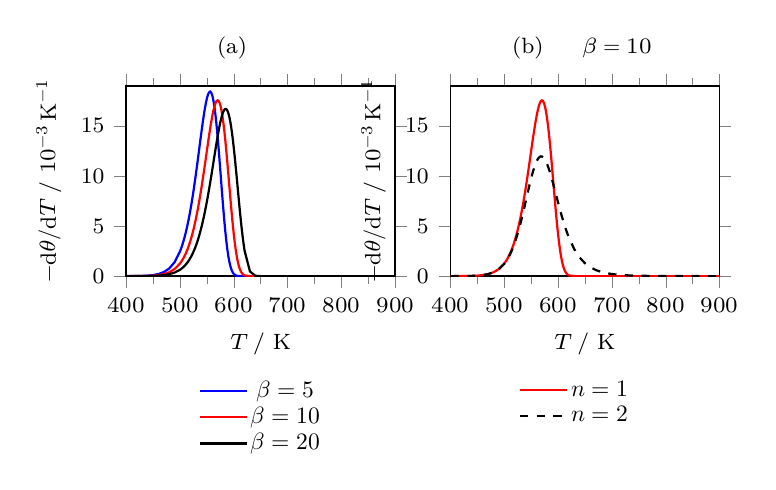
\begin{tikzpicture}
\begin{groupplot}[
  group style={group size=2 by 1, horizontal sep=7mm},
  width=50mm, height=40mm,
  xmin=400, xmax=900, ymin=0, ymax=0.019,
  xtick={400,500,600,700,800,900}, minor xtick={450,550,650,750,850},
  ytick={0,0.005,0.010,0.015}, yticklabels={0,5,10,15},
  scaled x ticks=false, scaled y ticks=false,   % 只保留 ylabel 里的一套倍率（R5-U01）
  xlabel={$T$ / K}, ylabel={$-\mathrm{d}\theta/\mathrm{d}T$ / $10^{-3}\,\unit{K^{-1}}$},
  tick label style={font=\srcsize}, label style={font=\srcsize},
  title style={font=\srcsize},
  legend style={font=\srcsize, draw=none, fill=none},
  every axis plot/.append style={thick},
]
\nextgroupplot[title={(a) 升温速率（一级）},
  legend style={at={(0.5,-0.50)}, anchor=north, legend columns=1,
                nodes={inner sep=1pt}}]
\addplot[blue, thick] table[row sep=\\, y index=1] {
%%  T/K      -dtheta/dT / K^{-1}
  400.0  1.88401e-06 \\
  410.0  4.54222e-06 \\
  420.0  1.05011e-05 \\
  430.0  2.33470e-05 \\
  440.0  5.00462e-05 \\
  450.0  1.03661e-04 \\
  460.0  2.07858e-04 \\
  470.0  4.04013e-04 \\
  480.0  7.61651e-04 \\
  490.0  1.39195e-03 \\
  500.0  2.46052e-03 \\
  502.0  2.74543e-03 \\
  504.0  3.05852e-03 \\
  506.0  3.40174e-03 \\
  508.0  3.77702e-03 \\
  510.0  4.18623e-03 \\
  512.0  4.63108e-03 \\
  514.0  5.11311e-03 \\
  516.0  5.63357e-03 \\
  518.0  6.19336e-03 \\
  520.0  6.79287e-03 \\
  522.0  7.43194e-03 \\
  524.0  8.10962e-03 \\
  526.0  8.82411e-03 \\
  528.0  9.57257e-03 \\
  530.0  1.03509e-02 \\
  532.0  1.11536e-02 \\
  534.0  1.19738e-02 \\
  536.0  1.28026e-02 \\
  538.0  1.36297e-02 \\
  540.0  1.44424e-02 \\
  542.0  1.52267e-02 \\
  544.0  1.59663e-02 \\
  546.0  1.66435e-02 \\
  548.0  1.72394e-02 \\
  550.0  1.77341e-02 \\
  552.0  1.81075e-02 \\
  554.0  1.83404e-02 \\
  556.0  1.84149e-02 \\
  558.0  1.83158e-02 \\
  560.0  1.80319e-02 \\
  562.0  1.75569e-02 \\
  564.0  1.68909e-02 \\
  566.0  1.60409e-02 \\
  568.0  1.50213e-02 \\
  570.0  1.38546e-02 \\
  572.0  1.25705e-02 \\
  574.0  1.12047e-02 \\
  576.0  9.79745e-03 \\
  578.0  8.39110e-03 \\
  580.0  7.02740e-03 \\
  582.0  5.74464e-03 \\
  584.0  4.57496e-03 \\
  586.0  3.54217e-03 \\
  588.0  2.66040e-03 \\
  590.0  1.93369e-03 \\
  592.0  1.35668e-03 \\
  594.0  9.16292e-04 \\
  596.0  5.93995e-04 \\
  598.0  3.68435e-04 \\
  600.0  2.17927e-04 \\
  602.0  1.22483e-04 \\
  604.0  6.51608e-05 \\
  606.0  3.26787e-05 \\
  608.0  1.53819e-05 \\
  610.0  6.76378e-06 \\
  612.0  2.76466e-06 \\
  614.0  1.04486e-06 \\
  616.0  3.63060e-07 \\
  618.0  1.15287e-07 \\
  620.0  3.32409e-08 \\
  630.0  1.20687e-11 \\
  640.0  1.14507e-16 \\
  650.0  0.00000e+00 \\
  660.0  0.00000e+00 \\
  670.0  0.00000e+00 \\
  680.0  0.00000e+00 \\
  690.0  0.00000e+00 \\
  700.0  0.00000e+00 \\
  710.0  0.00000e+00 \\
  720.0  0.00000e+00 \\
  730.0  0.00000e+00 \\
  740.0  0.00000e+00 \\
  750.0  0.00000e+00 \\
  760.0  0.00000e+00 \\
  770.0  0.00000e+00 \\
  780.0  0.00000e+00 \\
  790.0  0.00000e+00 \\
  800.0  0.00000e+00 \\
  810.0  0.00000e+00 \\
  820.0  0.00000e+00 \\
  830.0  0.00000e+00 \\
  840.0  0.00000e+00 \\
  850.0  0.00000e+00 \\
  860.0  0.00000e+00 \\
  870.0  0.00000e+00 \\
  880.0  0.00000e+00 \\
  890.0  0.00000e+00 \\
  900.0  0.00000e+00 \\
};\addlegendentry{$\beta=5$}
\addplot[red, thick] table[row sep=\\, y index=1] {
%%  T/K      -dtheta/dT / K^{-1}
  400.0  9.42017e-07 \\
  410.0  2.27117e-06 \\
  420.0  5.25087e-06 \\
  430.0  1.16752e-05 \\
  440.0  2.50310e-05 \\
  450.0  5.18663e-05 \\
  460.0  1.04079e-04 \\
  470.0  2.02598e-04 \\
  480.0  3.83032e-04 \\
  490.0  7.03750e-04 \\
  500.0  1.25614e-03 \\
  502.0  1.40541e-03 \\
  504.0  1.57046e-03 \\
  506.0  1.75267e-03 \\
  508.0  1.95348e-03 \\
  510.0  2.17440e-03 \\
  512.0  2.41698e-03 \\
  514.0  2.68282e-03 \\
  516.0  2.97355e-03 \\
  518.0  3.29076e-03 \\
  520.0  3.63605e-03 \\
  522.0  4.01094e-03 \\
  524.0  4.41683e-03 \\
  526.0  4.85498e-03 \\
  528.0  5.32642e-03 \\
  530.0  5.83188e-03 \\
  532.0  6.37174e-03 \\
  534.0  6.94591e-03 \\
  536.0  7.55375e-03 \\
  538.0  8.19391e-03 \\
  540.0  8.86430e-03 \\
  542.0  9.56186e-03 \\
  544.0  1.02825e-02 \\
  546.0  1.10211e-02 \\
  548.0  1.17709e-02 \\
  550.0  1.25242e-02 \\
  552.0  1.32716e-02 \\
  554.0  1.40021e-02 \\
  556.0  1.47035e-02 \\
  558.0  1.53622e-02 \\
  560.0  1.59632e-02 \\
  562.0  1.64908e-02 \\
  564.0  1.69285e-02 \\
  566.0  1.72600e-02 \\
  568.0  1.74694e-02 \\
  570.0  1.75421e-02 \\
  572.0  1.74656e-02 \\
  574.0  1.72306e-02 \\
  576.0  1.68312e-02 \\
  578.0  1.62665e-02 \\
  580.0  1.55410e-02 \\
  582.0  1.46650e-02 \\
  584.0  1.36548e-02 \\
  586.0  1.25326e-02 \\
  588.0  1.13259e-02 \\
  590.0  1.00661e-02 \\
  592.0  8.78720e-03 \\
  594.0  7.52408e-03 \\
  596.0  6.31005e-03 \\
  598.0  5.17498e-03 \\
  600.0  4.14336e-03 \\
  602.0  3.23287e-03 \\
  604.0  2.45348e-03 \\
  606.0  1.80737e-03 \\
  608.0  1.28953e-03 \\
  610.0  8.89040e-04 \\
  612.0  5.90796e-04 \\
  614.0  3.77421e-04 \\
  616.0  2.31131e-04 \\
  618.0  1.35277e-04 \\
  620.0  7.54274e-05 \\
  630.0  1.72886e-06 \\
  640.0  6.37182e-09 \\
  650.0  1.87666e-12 \\
  660.0  1.74736e-17 \\
  670.0  0.00000e+00 \\
  680.0  0.00000e+00 \\
  690.0  0.00000e+00 \\
  700.0  0.00000e+00 \\
  710.0  0.00000e+00 \\
  720.0  0.00000e+00 \\
  730.0  0.00000e+00 \\
  740.0  0.00000e+00 \\
  750.0  0.00000e+00 \\
  760.0  0.00000e+00 \\
  770.0  0.00000e+00 \\
  780.0  0.00000e+00 \\
  790.0  0.00000e+00 \\
  800.0  0.00000e+00 \\
  810.0  0.00000e+00 \\
  820.0  0.00000e+00 \\
  830.0  0.00000e+00 \\
  840.0  0.00000e+00 \\
  850.0  0.00000e+00 \\
  860.0  0.00000e+00 \\
  870.0  0.00000e+00 \\
  880.0  0.00000e+00 \\
  890.0  0.00000e+00 \\
  900.0  0.00000e+00 \\
};\addlegendentry{$\beta=10$}
\addplot[black, thick] table[row sep=\\, y index=1] {
%%  T/K      -dtheta/dT / K^{-1}
  400.0  4.71011e-07 \\
  410.0  1.13560e-06 \\
  420.0  2.62551e-06 \\
  430.0  5.83800e-06 \\
  440.0  1.25175e-05 \\
  450.0  2.59421e-05 \\
  460.0  5.20769e-05 \\
  470.0  1.01447e-04 \\
  480.0  1.92070e-04 \\
  490.0  3.53835e-04 \\
  500.0  6.34643e-04 \\
  502.0  7.11023e-04 \\
  504.0  7.95737e-04 \\
  506.0  8.89579e-04 \\
  508.0  9.93399e-04 \\
  510.0  1.10811e-03 \\
  512.0  1.23468e-03 \\
  514.0  1.37414e-03 \\
  516.0  1.52758e-03 \\
  518.0  1.69616e-03 \\
  520.0  1.88106e-03 \\
  522.0  2.08355e-03 \\
  524.0  2.30489e-03 \\
  526.0  2.54642e-03 \\
  528.0  2.80946e-03 \\
  530.0  3.09534e-03 \\
  532.0  3.40537e-03 \\
  534.0  3.74079e-03 \\
  536.0  4.10278e-03 \\
  538.0  4.49241e-03 \\
  540.0  4.91056e-03 \\
  542.0  5.35792e-03 \\
  544.0  5.83490e-03 \\
  546.0  6.34159e-03 \\
  548.0  6.87766e-03 \\
  550.0  7.44229e-03 \\
  552.0  8.03411e-03 \\
  554.0  8.65108e-03 \\
  556.0  9.29039e-03 \\
  558.0  9.94840e-03 \\
  560.0  1.06205e-02 \\
  562.0  1.13011e-02 \\
  564.0  1.19836e-02 \\
  566.0  1.26599e-02 \\
  568.0  1.33213e-02 \\
  570.0  1.39576e-02 \\
  572.0  1.45575e-02 \\
  574.0  1.51089e-02 \\
  576.0  1.55991e-02 \\
  578.0  1.60146e-02 \\
  580.0  1.63420e-02 \\
  582.0  1.65682e-02 \\
  584.0  1.66809e-02 \\
  586.0  1.66691e-02 \\
  588.0  1.65242e-02 \\
  590.0  1.62398e-02 \\
  592.0  1.58133e-02 \\
  594.0  1.52457e-02 \\
  596.0  1.45426e-02 \\
  598.0  1.37141e-02 \\
  600.0  1.27749e-02 \\
  602.0  1.17444e-02 \\
  604.0  1.06455e-02 \\
  606.0  9.50434e-03 \\
  608.0  8.34884e-03 \\
  610.0  7.20729e-03 \\
  612.0  6.10689e-03 \\
  614.0  5.07218e-03 \\
  616.0  4.12366e-03 \\
  618.0  3.27666e-03 \\
  620.0  2.54064e-03 \\
  630.0  4.62693e-04 \\
  640.0  3.35950e-05 \\
  650.0  6.85760e-07 \\
  660.0  2.46950e-09 \\
  670.0  8.47768e-13 \\
  680.0  1.24784e-17 \\
  690.0  0.00000e+00 \\
  700.0  0.00000e+00 \\
  710.0  0.00000e+00 \\
  720.0  0.00000e+00 \\
  730.0  0.00000e+00 \\
  740.0  0.00000e+00 \\
  750.0  0.00000e+00 \\
  760.0  0.00000e+00 \\
  770.0  0.00000e+00 \\
  780.0  0.00000e+00 \\
  790.0  0.00000e+00 \\
  800.0  0.00000e+00 \\
  810.0  0.00000e+00 \\
  820.0  0.00000e+00 \\
  830.0  0.00000e+00 \\
  840.0  0.00000e+00 \\
  850.0  0.00000e+00 \\
  860.0  0.00000e+00 \\
  870.0  0.00000e+00 \\
  880.0  0.00000e+00 \\
  890.0  0.00000e+00 \\
  900.0  0.00000e+00 \\
};\addlegendentry{$\beta=20$}
\nextgroupplot[title={(b) 脱附级数（$\beta=10$）},
  legend style={at={(0.5,-0.50)}, anchor=north, legend columns=1,
                nodes={inner sep=1pt}}]
\addplot[red, thick] table[row sep=\\, y index=1] {
%%  T/K      -dtheta/dT / K^{-1}
  400.0  9.42017e-07 \\
  410.0  2.27117e-06 \\
  420.0  5.25087e-06 \\
  430.0  1.16752e-05 \\
  440.0  2.50310e-05 \\
  450.0  5.18663e-05 \\
  460.0  1.04079e-04 \\
  470.0  2.02598e-04 \\
  480.0  3.83032e-04 \\
  490.0  7.03750e-04 \\
  500.0  1.25614e-03 \\
  502.0  1.40541e-03 \\
  504.0  1.57046e-03 \\
  506.0  1.75267e-03 \\
  508.0  1.95348e-03 \\
  510.0  2.17440e-03 \\
  512.0  2.41698e-03 \\
  514.0  2.68282e-03 \\
  516.0  2.97355e-03 \\
  518.0  3.29076e-03 \\
  520.0  3.63605e-03 \\
  522.0  4.01094e-03 \\
  524.0  4.41683e-03 \\
  526.0  4.85498e-03 \\
  528.0  5.32642e-03 \\
  530.0  5.83188e-03 \\
  532.0  6.37174e-03 \\
  534.0  6.94591e-03 \\
  536.0  7.55375e-03 \\
  538.0  8.19391e-03 \\
  540.0  8.86430e-03 \\
  542.0  9.56186e-03 \\
  544.0  1.02825e-02 \\
  546.0  1.10211e-02 \\
  548.0  1.17709e-02 \\
  550.0  1.25242e-02 \\
  552.0  1.32716e-02 \\
  554.0  1.40021e-02 \\
  556.0  1.47035e-02 \\
  558.0  1.53622e-02 \\
  560.0  1.59632e-02 \\
  562.0  1.64908e-02 \\
  564.0  1.69285e-02 \\
  566.0  1.72600e-02 \\
  568.0  1.74694e-02 \\
  570.0  1.75421e-02 \\
  572.0  1.74656e-02 \\
  574.0  1.72306e-02 \\
  576.0  1.68312e-02 \\
  578.0  1.62665e-02 \\
  580.0  1.55410e-02 \\
  582.0  1.46650e-02 \\
  584.0  1.36548e-02 \\
  586.0  1.25326e-02 \\
  588.0  1.13259e-02 \\
  590.0  1.00661e-02 \\
  592.0  8.78720e-03 \\
  594.0  7.52408e-03 \\
  596.0  6.31005e-03 \\
  598.0  5.17498e-03 \\
  600.0  4.14336e-03 \\
  602.0  3.23287e-03 \\
  604.0  2.45348e-03 \\
  606.0  1.80737e-03 \\
  608.0  1.28953e-03 \\
  610.0  8.89040e-04 \\
  612.0  5.90796e-04 \\
  614.0  3.77421e-04 \\
  616.0  2.31131e-04 \\
  618.0  1.35277e-04 \\
  620.0  7.54274e-05 \\
  630.0  1.72886e-06 \\
  640.0  6.37182e-09 \\
  650.0  1.87666e-12 \\
  660.0  1.74736e-17 \\
  670.0  0.00000e+00 \\
  680.0  0.00000e+00 \\
  690.0  0.00000e+00 \\
  700.0  0.00000e+00 \\
  710.0  0.00000e+00 \\
  720.0  0.00000e+00 \\
  730.0  0.00000e+00 \\
  740.0  0.00000e+00 \\
  750.0  0.00000e+00 \\
  760.0  0.00000e+00 \\
  770.0  0.00000e+00 \\
  780.0  0.00000e+00 \\
  790.0  0.00000e+00 \\
  800.0  0.00000e+00 \\
  810.0  0.00000e+00 \\
  820.0  0.00000e+00 \\
  830.0  0.00000e+00 \\
  840.0  0.00000e+00 \\
  850.0  0.00000e+00 \\
  860.0  0.00000e+00 \\
  870.0  0.00000e+00 \\
  880.0  0.00000e+00 \\
  890.0  0.00000e+00 \\
  900.0  0.00000e+00 \\
};\addlegendentry{$n=1$，拖尾}
\addplot[black, dashed, thick] table[row sep=\\, y index=1] {
%%  T/K      -dtheta/dT / K^{-1}
  400.0  9.42007e-07 \\
  410.0  2.27111e-06 \\
  420.0  5.25055e-06 \\
  430.0  1.16735e-05 \\
  440.0  2.50231e-05 \\
  450.0  5.18307e-05 \\
  460.0  1.03929e-04 \\
  470.0  2.02008e-04 \\
  480.0  3.80838e-04 \\
  490.0  6.96062e-04 \\
  500.0  1.23079e-03 \\
  502.0  1.37347e-03 \\
  504.0  1.53032e-03 \\
  506.0  1.70237e-03 \\
  508.0  1.89063e-03 \\
  510.0  2.09608e-03 \\
  512.0  2.31968e-03 \\
  514.0  2.56232e-03 \\
  516.0  2.82477e-03 \\
  518.0  3.10770e-03 \\
  520.0  3.41157e-03 \\
  522.0  3.73666e-03 \\
  524.0  4.08297e-03 \\
  526.0  4.45020e-03 \\
  528.0  4.83766e-03 \\
  530.0  5.24431e-03 \\
  532.0  5.66859e-03 \\
  534.0  6.10850e-03 \\
  536.0  6.56148e-03 \\
  538.0  7.02443e-03 \\
  540.0  7.49374e-03 \\
  542.0  7.96522e-03 \\
  544.0  8.43422e-03 \\
  546.0  8.89566e-03 \\
  548.0  9.34411e-03 \\
  550.0  9.77393e-03 \\
  552.0  1.01794e-02 \\
  554.0  1.05547e-02 \\
  556.0  1.08945e-02 \\
  558.0  1.11937e-02 \\
  560.0  1.14476e-02 \\
  562.0  1.16526e-02 \\
  564.0  1.18055e-02 \\
  566.0  1.19043e-02 \\
  568.0  1.19480e-02 \\
  570.0  1.19364e-02 \\
  572.0  1.18706e-02 \\
  574.0  1.17523e-02 \\
  576.0  1.15845e-02 \\
  578.0  1.13707e-02 \\
  580.0  1.11149e-02 \\
  582.0  1.08220e-02 \\
  584.0  1.04967e-02 \\
  586.0  1.01442e-02 \\
  588.0  9.76968e-03 \\
  590.0  9.37818e-03 \\
  592.0  8.97452e-03 \\
  594.0  8.56324e-03 \\
  596.0  8.14853e-03 \\
  598.0  7.73416e-03 \\
  600.0  7.32347e-03 \\
  602.0  6.91935e-03 \\
  604.0  6.52427e-03 \\
  606.0  6.14026e-03 \\
  608.0  5.76895e-03 \\
  610.0  5.41161e-03 \\
  612.0  5.06916e-03 \\
  614.0  4.74225e-03 \\
  616.0  4.43124e-03 \\
  618.0  4.13629e-03 \\
  620.0  3.85733e-03 \\
  630.0  2.69163e-03 \\
  640.0  1.85816e-03 \\
  650.0  1.27815e-03 \\
  660.0  8.80104e-04 \\
  670.0  6.08440e-04 \\
  680.0  4.23081e-04 \\
  690.0  2.96222e-04 \\
  700.0  2.08956e-04 \\
  710.0  1.48545e-04 \\
  720.0  1.06430e-04 \\
  730.0  7.68510e-05 \\
  740.0  5.59197e-05 \\
  750.0  4.09954e-05 \\
  760.0  3.02743e-05 \\
  770.0  2.25158e-05 \\
  780.0  1.68609e-05 \\
  790.0  1.27104e-05 \\
  800.0  9.64323e-06 \\
  810.0  7.36178e-06 \\
  820.0  5.65389e-06 \\
  830.0  4.36747e-06 \\
  840.0  3.39270e-06 \\
  850.0  2.64980e-06 \\
  860.0  2.08044e-06 \\
  870.0  1.64171e-06 \\
  880.0  1.30187e-06 \\
  890.0  1.03728e-06 \\
  900.0  8.30270e-07 \\
};\addlegendentry{$n=2$，对称}
\end{groupplot}
\end{tikzpicture}
\caption{TPD 谱的模型计算：\textbf{峰面积标定吸附量，峰位标定动力学}。曲线由
Polanyi--Wigner 方程数值求解，取相同初始覆盖度 $\theta_0=1$（饱和）、
$E_d=\qty{120}{kJ.mol^{-1}}$、$A=\qty{7.35e8}{s^{-1}}$（$=\qty{4.41e10}{min^{-1}}$；
由 $n=1$、$\beta=\qty{10}{K.min^{-1}}$、$T_p=\qty{570.000}{K}$ 的解析峰温条件标定）、
$T_0=\qty{300}{K}$。纵轴为正脱附速率 $-\mathrm{d}\theta/\mathrm{d}T$，即把按时间计的
脱附速率 $-\mathrm{d}\theta/\mathrm{d}t$ 除以 $\beta$：脱附使 $\theta$ 随 $T$ 下降，加负号后
曲线为正，与式~\eqref{eq:ch05-peak} 的导数符号约定一致。\textbf{(a)} 一级脱附，$\beta$ 由 $5$ 增到
$\qty{20}{K.min^{-1}}$：峰温由 $556$ 右移到 $\qty{585}{K}$（约 $\qty{29}{K}$），
而三条曲线下的面积\textbf{完全相同}
（$\int(-\mathrm{d}\theta/\mathrm{d}T)\,\mathrm{d}T=\theta_0=1.0000$）——
\textbf{面积并不随 $\beta$ 成倍放大}，这正是「峰面积标定吸附量」的依据；
按时间计的速率 $-\mathrm{d}\theta/\mathrm{d}t$ 才随 $\beta$ 成比例放大，两者只差因子
$\beta$，故比较升温速率只能看峰位、不能看峰高。\textbf{(b)} 固定
$\beta=\qty{10}{K.min^{-1}}$ 只改脱附级数：$n=2$ 的峰比 $n=1$ \textbf{更低更宽}——
峰高比 $0.681$，半高全宽由 $52.3$ 增至 $\qty{73.5}{K}$（约 $1.4$ 倍）——
峰位略向低温移（$568.6$ 对 $\qty{570.0}{K}$），峰面积仍是 $1.0000$
（初始覆盖度相同）。局限：只含一级与二级脱附、单一均匀表面与恒定 $\beta$，
未含再吸附、扩散与检测器响应，不可用于直接读数值。横轴两端之外仍有极小尾部
（$\theta$ 的残余 $<10^{-6}$），上列积分按 $300$--$\qty{1500}{K}$ 全温区算得。\modelmark
\figsrc{据 S1 §5.3.1—5.3.3 原理自绘，书内 p.311—315 / PDF p.330—334；坐标表由
\texttt{tools/gen\_tpd\_table.py} 生成}}
\label{fig:ch05-tpd}
\end{figure}

\begin{pitfall}
\textbf{峰重叠。} 相邻位点的峰在半宽可比于峰间距时合并为一个宽峰，被读成「单一均匀位点」。
识别办法是改变升温速率或初始覆盖度：真实两峰的条件响应不同，单峰只整体平移。

\textbf{再吸附抬高峰温。} 载气流速过低、床层过厚或样品量过大时，脱附分子在床层内被重新
吸附，表现为峰温偏高、峰形拖尾，由峰温算得的 $E_d$ 系统性偏大。判据是把载气流速提高一档
重测：真实峰位基本不动，再吸附控制的峰位明显左移。

\textbf{载气流速与升温速率耦合。} 两者共同决定脱附物在检测器处的驻留时间与峰宽，单独优化
其一会得到假的最优条件；报告时必须同时给出 $\beta$、流速、装量和粒度。

\textbf{定量必须标定。} 热导或质谱信号是浓度而非摩尔量，峰面积只有经已知体积脉冲标定
（式~\eqref{eq:ch05-pulse}）后才能换算为吸附量；未标定就比较不同批次样品的峰面积，在
检测器灵敏度漂移时会得出错误的位点数目结论。
\end{pitfall}

\subsubsection{TPD 动力学参数的确定}

Cvetanović 和 Amenorinya 为简化理论处理提出四条假设：\textbf{不发生再吸附}、\textbf{脱附为
一级过程}、\textbf{表面均匀}、\textbf{不存在扩散}。此时脱附速率
$N = -\mathrm{d}\theta/\mathrm{d}t = k_d\,\theta^{\,n}$，$k_d$ 取式~\eqref{eq:ch05-kd}；
设线性升温 $T=T_0+\beta t$，峰顶处 $\mathrm{d}^2\theta/\mathrm{d}T^2=0$，解得峰温条件
\begin{equation}
\frac{E_d}{R\,T_m^{2}} = \frac{A}{\beta}\; n\,\theta_m^{\,n-1}
\exp\!\left(-\frac{E_d}{R\,T_m}\right)
\label{eq:ch05-peak}
\end{equation}
式中下标 $m$ 表示峰最高点处的量，其来源是 $\mathrm{d}\theta/\mathrm{d}T =
-(A/\beta)\,\theta^{\,n}\exp(-E_d/RT)$ 在峰顶处满足 $\mathrm{d}^2\theta/\mathrm{d}T^2=0$。
对一级脱附（$n=1$）$\theta_m$ 项消失，即得 Redhead 方程
\begin{equation}
\frac{E_d}{R\,T_m^{2}} = \frac{A}{\beta}\exp\!\left(-\frac{E_d}{R\,T_m}\right)
\label{eq:ch05-redhead}
\end{equation}
此处已对照原页面图像（书内 p.315 / PDF p.334）。原书不按 $n$ 阶通式起手，而是自
一级脱附出发，在峰顶处令 $\mathrm{d}C/\mathrm{d}T=0$，即
$\dfrac{\partial\theta}{\partial T}=\dfrac{V_sV_mA}{F}\cdot\dfrac{\mathrm{d}(\theta\mathrm{e}^{-E_d/RT})}{\mathrm{d}T}=0$，
从而 $\mathrm{d}(\theta\mathrm{e}^{-E_d/RT})/\mathrm{d}T=0$（式 5-52）；解此微分方程得
$(k_d)_M=\beta E_d/RT_M^2$（式 5-53），再由 $k_d=A\exp(-E_d/RT)$ 得
$(k_d)_M=A\exp(-E_d/RT_M)=\beta E_d/RT_M^2$（式 5-54）。原书并注明「这里 $M$ 指 TPD 峰的
最高点」。因此本稿的 $n\theta_m^{\,n-1}$ 因子与「先写 $n$ 阶、再退化到 $n=1$」的叙述层次
属本改编本为便于讨论非一级脱附而加，原书通篇按一级处理；两者在 $n=1$ 时一致。
原书同处另写「在已知加热速率 $\beta$ 时，假定指前因子 $A$ 也已知，从式 (5-54) 可看出，
脱附活化能和 $T_M$ 具有对应关系」，即该式在原书中是逐温度对应的隐式关系，本稿写成
$E_d/RT_m^{2}=(A/\beta)\exp(-E_d/RT_m)$ 属等价变形。原书未出现常数 3.64 的形式。

式~\eqref{eq:ch05-redhead} 是把\textbf{峰温}翻译成\textbf{脱附活化能}的唯一桥梁，它无解析
解、实用中按假定的 $A$ 值迭代求解；其可换算性完全取决于表~\ref{tab:ch05-redhead} 的四个前提。

\begin{table}[htbp]
\centering
\caption{由峰温换算脱附活化能的四个前提\src{前两条为 S1 §5.3.3 原书明确列出的简化假设（书内 p.313 / PDF p.332），后两条据书内 p.313—316 归纳。}}
\label{tab:ch05-redhead}
{\srcsize
\begin{tabularx}{\columnwidth}{@{}lXX@{}}
\toprule
前提 & 要求 & 被违反时的表现 \\
\midrule
一级脱附 & $n=1$，$\theta_m$ 项消失 & 二级脱附下 $E_d$ 随初始覆盖度变化 \\
不再吸附 & 原书简化假设①，正文式 (5-39)—(5-41) 已略去再吸附项 $k_aC(1-\theta)$ & 峰温偏高、拖尾，$E_d$ 系统性偏大 \\
指前因子已知 & 需假定 $A$（常见 $10^{13}\,\si{s^{-1}}$ 量级） & $E_d$ 与 $\ln A$ 强耦合：$A$ 差 2 个量级则 $E_d$ 差 $4.606\,RT_m$（$T_m=500$ K 时约 $19\,\si{kJ mol^{-1}}$）；本书表 5-3 自身算例的 $A$ 仅 $10^{4}\sim10^{5}\,\si{s^{-1}}$ \\
升温速率已知且恒定 & $\beta$ 线性、并在报告中给出 & 峰位漂移，变升温速率法斜率失效 \\
\bottomrule
\end{tabularx}}
\end{table}

\emph{核对说明}：已对照原页面图像（书内 p.313、p.315—316 / PDF p.332、p.334—335）。本表前两条（「一级脱附」「不再吸附」）对应原书 §5.3.3 开篇逐字列出的 Cvetanović 和 Amenomiya（1967）
四条简化假设中的假设①②，后两条（「指前因子已知」「升温速率已知且恒定」）系据书内 p.313—316 归纳，原书未单独列成表格（详见下文）。表中「$A$ 差 2 个量级则 $E_d$ 差 $4.606\,RT_m$」一句为改编本按 Redhead 近似式 $E_d=RT_m[\ln(AT_m/\beta)-3.64]$
对 $\ln A$ 求差所得：$\ln 100=4.606$，故 $\Delta E_d=R T_m\ln 100=4.606\,R T_m$（$T_m=500$ K 时约 $19\,\si{kJ mol^{-1}}$），原书未作此讨论。原稿此处写作「$E_d$ 约差 10\%」，该比例随 $E_d$ 水平漂移（$E_d=200$ 与 $100\,\si{kJ mol^{-1}}$ 时分别约 10\% 与 19\%），故改为给绝对量。
原书表 5-3 自身算例所印 $A$ 仅 $10^{4}\sim10^{5}\,\si{s^{-1}}$，与该前提并不自洽，
原书亦未就此展开讨论，本稿如实记录、不代为改动（逐值见下文）。

原书 §5.3.3 开篇（书内 p.313 / PDF p.332）逐字列出 Cvetanović 和 Amenomiya 于 1967 年提出的
四条简化假设：「①脱附过程不发生再吸附；②脱附为一级脱附过程；③固体表面是均匀的；
④不存在扩散过程」（假设①对应上表「不再吸附」，假设②对应「一级脱附」，假设③④为表面均匀
与无扩散，本稿未单列）。原书自式的起点为式 (5-39) $N=-\mathrm{d}\theta/\mathrm{d}t=k_d\theta-k_aC(1-\theta)$、
式 (5-40) $-V_m\mathrm{d}\theta/\mathrm{d}t=V_mk_d\theta-k_aC(1-\theta)$、
式 (5-41) $FC=V_s[V_mk_d\theta-k_aC(1-\theta)]$；本稿正文的
$N=-\mathrm{d}\theta/\mathrm{d}t=k_d\theta^{\,n}$ 是把式 (5-39) 在假设①下略去再吸附项、
并按本稿讨论非一级情形的需要改写为 $n$ 阶形式，原书只取一级。

\begin{measure}
\textbf{变升温速率法（不假定 $A$）。} 若不作 $A$ 的假设，可由式~\eqref{eq:ch05-redhead}
整理出：以 $2\ln T_m - \ln\beta$ 对 $1/T_m$ 作图，斜率为 $E_d/R$，由此得到脱附活化能。
实验上需在多个 $\beta$ 下各测一条 TPD 曲线、读出各自的 $T_m$ 后作图。原书给出烯烃在
氧化铝中心上脱附的实例（\ce{C2H4}、\ce{C3H6}、\ce{C4H8}），所得 $E_d$ 与 $A$ 列于其表 5-3；
作者同时指出该法实验工作量较大，并提到用谱线重叠法从单条 TPD 谱线求 $E_d$ 与 $A$ 的
替代途径\textsuperscript{\src{S1 §5.3.3，书内 p.315—316 / PDF p.334—335}}。
此处已对照原页面图像（书内 p.315—316 / PDF p.334—335）。原书式
(5-53) $(k_d)_M=\beta E_d/RT_M^2$、式 (5-54) $(k_d)_M=A\exp(-E_d/RT_M)=\beta E_d/RT_M^2$，
下标 $M$ 指 TPD 峰最高点；式 (5-55) 写作
$2\ln T_M-\ln\beta=E_d/RT_M+\ln(E_d/AR)$，即截距并非零而是 $\ln(E_d/AR)$，
本稿以「斜率即 $E_d/R$」概括、略去截距项，属改写。原书表 5-3「烯烃在 \ce{Al2O3} 上
脱附活化能（kcal/mol）和指前因子（$A$）」逐值核对：\ce{C2H4} $E_d=26.8$、$A=1.6\times10^5$；
\ce{C3H6} $E_d=14.2$、$A=6.8\times10^5$；\ce{C4H8} $E_d=12.1$、$A=1.2\times10^4$
（$E_d$ 单位确为 kcal/mol）。三组 $A$ 值确如原书所印、并非 OCR 失真，且远低于
常用假定 $10^{13}\,\si{s^{-1}}$——即\textbf{原书自身的算例并不满足其表 5-3 前提中的
「指前因子已知且合理」一条}，此处如实记录原书数值，不代为改动。
另据 p.316（PDF p.335）原文，该法「需测定不同升温速率 $\beta$ 时的峰顶温度 $T_M$，
用作图法求脱附活化能 $E_d$ 和指前因子 $A$，因此实验工作量较大」，并提到杨上闰用
谱线重叠法由一条 TPD 谱线求得 $E_d$ 与 $A$（文献[6]）。
\end{measure}

\subsubsection{程序升温还原（TPR）原理}

等温条件下的还原过程一般用成核模型和球收缩模型解释。以球形金属氧化物与 \ce{H2} 反应生成
金属和 \ce{H2O} 为例：\textbf{成核模型}认为反应从成核开始，随核长大与新核形成，金属核与
氧化物之间的反应界面增加、速率加快；核相互接触后界面变小、速率减慢，故 $\alpha$–$t$ 曲线
呈 S 形、$\mathrm{d}\alpha/\mathrm{d}t$ 先增后减。\textbf{球收缩模型}认为迅速成核形成很薄的
金属层后界面不断缩小、速率单调下降；两者区别在于成核速度。

程序升温条件下还原写作 $\ce{G + S -> P}$（\ce{G} 为 \ce{H2}，\ce{S} 为氧化物，\ce{P} 为
产物），速率与 Arrhenius 温度依赖、线性升温的关系为
\begin{equation}
r = \frac{\mathrm{d}\alpha}{\mathrm{d}t} = k\,f(\alpha),\qquad
k = A\exp\!\left(-\frac{E_a}{RT}\right),\qquad
\beta = \frac{\mathrm{d}T}{\mathrm{d}t}
\label{eq:ch05-tpr}
\end{equation}
式中 $\alpha$ 为还原分数。因 $\mathrm{d}/\mathrm{d}t = \beta\,\mathrm{d}/\mathrm{d}T$，
反应与气体浓度无关时有
$\mathrm{d}\alpha/\mathrm{d}T = (A/\beta)(1-\alpha)^{q}\exp(-E_a/RT)$。峰顶处
$\mathrm{d}[G]/\mathrm{d}T = 0$，整理、取对数并假定固体反应级数 $q=1$，得
\begin{equation}
2\ln T_m - \ln\beta + p\ln[G]_M + (q-1)\ln[S]_M = \frac{E_a}{R\,T_m} + \text{常数}
\label{eq:ch05-tpr-peak}
\end{equation}
式中 $p$、$q$ 分别为气体与固体的反应级数，$[G]_M$ 为峰顶处还原气浓度，$[S]_M$ 为峰顶处
固体浓度。已知 $p$、$q$ 时以式~\eqref{eq:ch05-tpr-peak} 左边对 $1/T_m$ 作图，斜率即 $E_a/R$。
由于固体反应级数通常为分数且该式对 $q$ 不敏感，原书进而\textbf{假定 $q=1$}，得化简式
\begin{equation}
2\ln T_m - \ln\beta + p\ln[G]_M = \frac{E_a}{R\,T_m} + \text{常数}
\label{eq:ch05-tpr-peak-q1}
\end{equation}
此处已对照原页面图像（书内 p.319 / PDF p.338）：原书式 (5-70)
$0=E/RT_M^2+q\,\mathrm{d}[S]_M/([S]_M\mathrm{d}T)$、式 (5-71)
$E/RT_M^2=[A[G]_M^p q[S]_M^{q-1}\exp(-E/RT)]/\beta$、式 (5-72) 即上式、
式 (5-73) 即化简式，逐字一致。原书另注：对 \ce{CuO} 还原发现 $p=0$ 时 $E$ 与
\ce{H2} 浓度有关，而 $p=1$ 时 $E$ 与浓度无关。

原书指出该法有两个实务限制。其一，\textbf{它并不实用}：实验拿到的 TPR 信息大多是还原气
（如 \ce{H2}）浓度与温度的关系、谱图由几个峰组成，而非 $\alpha$–$T$ 曲线本身；对流动体系
还原过程表现为 $\Delta[G] = [G]_{\text{进}} - [G]_{\text{出}}$，假定活塞流时低转化率下可由
$r = f\,[G]x$ 描述。其二，\textbf{氢溢流}：在某一物质表面形成的活性物种转移到在相同条件下
自身不能吸附或不能形成活性物种的另一物质表面。多组分催化剂中易还原的氧化物先在较低温度
还原成金属，若该金属能解离活化 \ce{H2}，原子氢便经金属—氧化物界面溢流到氧化物表面使之
还原；原子氢还原性强于分子氢，故存在氢溢流时氧化物还原温度明显降低。\ce{Pt}、\ce{Pd}、
\ce{Ag}、\ce{Cu}、\ce{Ni} 等均有此功能，贵金属作用尤其突出。

\begin{crosscheck}
氢溢流使 TPR 图谱难以按单一还原步骤归属：一个低温峰可能不代表该物种本身易还原，而代表
邻近金属提供了溢流通道。因此\textbf{TPR 的峰归属必须与 XRD、\ce{H2} 消耗量（定量）以及
\ce{CO}-TPR 回查}。原书明确指出，为消除氢溢流影响可选用溢流作用较小的 \ce{CO} 替代
\ce{H2} 作还原气，即 \ce{CO}-TPR\textsuperscript{\src{S1 §5.3.4，书内 p.316—319 /
PDF p.335—338}}。
\end{crosscheck}

\subsubsection{程序升温氧化（TPO）原理}

程序升温氧化的原理与 TPR 基本类似，是在一定升温速率下用氧化性气体（如 \ce{O2}）对催化剂
及其表面物种进行氧化的过程，主要用于研究催化剂表面积炭物种的生成机理。

\begin{principle}
与 TPD 的对应关系可以直接迁移：TPO 谱的峰面积对应\textbf{可氧化物种（积炭）的总量}，
峰温对应\textbf{该物种被氧化的难易程度}（积炭越石墨化、越难氧化，峰温越高），
峰数目对应\textbf{积炭物种的类别数}。因此 TPO 与 TPD 的全部定量前提——标定、载气流速、
升温速率、峰重叠——同样适用，且因为反应产物是 \ce{CO2}/\ce{CO}，需用质谱同时监测
两个通道以避免把部分氧化产物计漏。
\end{principle}

\srcnote{本节（5.1—5.3）据 S1 上册第 5 章，书内 p.301—319 / PDF p.320—338。化学吸附应用、
活性位与分散度测定、TPD/TPR/TPO 在具体体系中的应用见本章后续分片。原文中的
图 5-2—5-7 为原书谱图与装置流程图，因无图像核对能力未裁图，本分片仅以
\modelmark 模型计算图替代。}
}{}
\IfFileExists{chapters/parts/ch05-b.tex}{\subsection{TPD 谱的三层信息：峰数、峰温与峰面积}
\label{sec:ch05b-read}

\begin{probout}
分片 a 建立了 TPD 的动力学基础与三种吸附等温式，本节不再重复，转而处理实际操作中最容易被跳过的一步——
\emph{把一张 TPD 谱读成结论}。一张谱图只提供三条可以独立读取的信息：峰数、峰温、峰面积。
本节回答：这三条信息各自指向什么结论、结论成立需要什么前提、以及在什么条件下这个指向会彻底失效。
判读的目标不是「数出几个峰就报几个物种」，而是给出「观测—前提—推断」三段式结论。
\end{probout}

\begin{principle}
\textbf{峰面积给出脱附量。} 检测器信号 $A(T)$ 与载气中脱附物种的浓度成正比。设载气总摩尔流率为 $F$
（mol\,s$^{-1}$）、标定因子 $k_A$（使浓度 $c=A/k_A$）、升温速率 $\beta=\mathrm{d}T/\mathrm{d}t$、样品质量 $m$，
则单位质量样品的脱附量为
\begin{equation}
\frac{n_{\mathrm{des}}}{m}
=\frac{F}{k_A\,\beta\,m}\int_{T_1}^{T_2} A(T)\,\mathrm{d}T .
\label{eq:ch05b-area}
\end{equation}
式中 $F/(k_A\beta m)$ 是几个量拧在一起的总标定常数：实践中不逐个测定，而是用已知量的标样整体标定
（\S\ref{sec:ch05b-quant}）。积分窗口 $[T_1,T_2]$ 必须等信号回到基线之后才关闭；窗口开得不够宽，
高温尾部被切掉，脱附量会系统性偏低，而这一点在谱图上完全看不出来。

\textbf{峰温给出脱附活化能。} 对一级脱附，Polanyi--Wigner 速率式
$\mathrm{d}\theta/\mathrm{d}t=-\nu\theta\exp[-E_{\mathrm d}/(RT)]$ 在峰顶满足
$\mathrm{d}^{2}\theta/\mathrm{d}T^{2}=0$，用 $\beta$ 换元后得
\begin{equation}
\frac{E_{\mathrm d}}{R T_{\mathrm p}^{2}}
=\frac{\nu}{\beta}\exp\!\left(-\frac{E_{\mathrm d}}{R T_{\mathrm p}}\right)
\quad\Longrightarrow\quad
\frac{E_{\mathrm d}}{R T_{\mathrm p}}
=\ln\frac{\nu T_{\mathrm p}}{\beta}-3.64 ,
\label{eq:ch05b-redhead}
\end{equation}
即通常所说的 Redhead 式。右端的 $3.64$ 来自 $\ln[E_{\mathrm d}/(RT_{\mathrm p})]$ 在常见参数区间内的近似取值，
所以 \equref{eq:ch05b-redhead} 是\emph{近似式}，而且 $\nu$ 必须事先指定（常用 $10^{13}\,\mathrm{s^{-1}}$）。
对 \equref{eq:ch05b-redhead} 求微分，得到两条后面反复用到的灵敏度关系：
\begin{equation}
\frac{\partial T_{\mathrm p}}{\partial\ln\beta}=\frac{R T_{\mathrm p}^{2}}{E_{\mathrm d}},
\qquad
\delta E_{\mathrm d}=R T_{\mathrm p}\,\delta\ln\nu .
\label{eq:ch05b-sens}
\end{equation}
\end{principle}

\begin{measure}
取 $E_{\mathrm d}=\qty{120}{kJ.mol^{-1}}$、$\nu=10^{13}\,\mathrm{s^{-1}}$，数值求解
\equref{eq:ch05b-redhead} 得 $T_{\mathrm p}\approx 423$ K（$\beta=10$ K\,min$^{-1}$）。
由 \equref{eq:ch05b-sens}：

\begin{itemize}
  \item 升温速率从 10 提高到 40 K\,min$^{-1}$（$\ln 4=1.386$），
        $\Delta T_{\mathrm p}\approx(8.314\times423^{2}/120000)\times1.386\approx 17$ K。
        也就是说，两个实验室只要升温速率不同，同一催化剂也可以差出十几开——这属于仪器差异，不是化学差异。
  \item 峰温测量误差 $\pm5$ K 只带来 $\pm1.4$ kJ\,mol$^{-1}$ 的 $E_{\mathrm d}$ 误差，可以忽略；
        真正的不确定度来自 $\nu$：$\nu$ 从 $10^{12}$ 改到 $10^{14}$（$\delta\ln\nu=4.6$）会使
        $E_{\mathrm d}$ 变动 $8.314\times423\times4.6\approx\qty{16}{kJ.mol^{-1}}$，
        即单张 TPD 谱给出的 $E_{\mathrm d}$ 精度大约只有 $\pm10\%$，而这还是在假定模型正确的前提下。
\end{itemize}

因此本节后续一律要求：\emph{报告 $E_{\mathrm d}$ 时必须同时报告所用的 $\nu$、升温速率和是否做过变速率校正}；
只报一个数而不报条件，等于没有报。
\end{measure}

要求 1 的核心结论由图~\ref{fig:ch05b-tpd-model} 概括：升温速率与再吸附都不改变脱附量，
但它们强烈改变峰形，所以\emph{峰高、峰宽、峰温都不能当作吸附量的量度，只有峰面积可以}。

\begin{figure}[htbp]
\centering
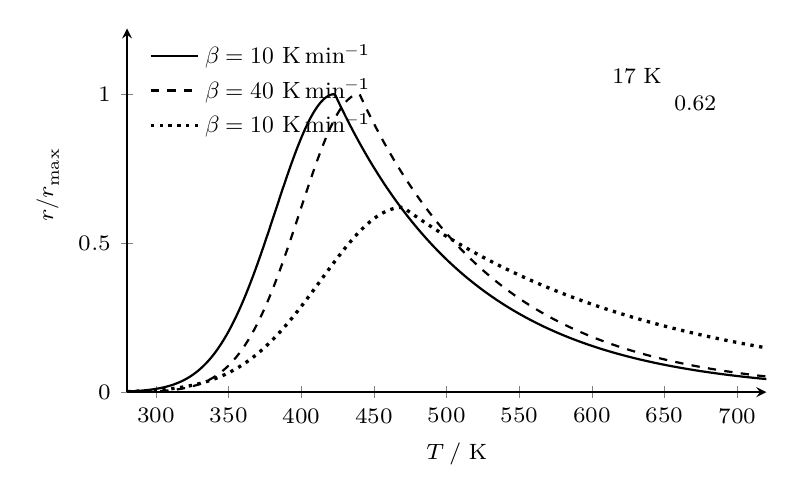
\begin{tikzpicture}
\tikzset{declare function={
  fA(\t) = \t < 423 ? exp(-((\t-423)/58)*((\t-423)/58)) : exp(-(\t-423)/95);
  fB(\t) = \t < 440 ? exp(-((\t-440)/58)*((\t-440)/58)) : exp(-(\t-440)/95);
  fC(\t) = \t < 470 ? 0.62*exp(-((\t-470)/80)*((\t-470)/80)) : 0.62*exp(-(\t-470)/175);
}}
\begin{axis}[
  width=\onecolwidth,
  height=62mm,
  xmin=280, xmax=720, ymin=0, ymax=1.22,
  xlabel={温度 $T$ / K},
  ylabel={归一化脱附速率 $r/r_{\max}$},
  axis lines=left,
  tick label style={font={\fontsize{8}{9.6}\selectfont}},
  label style={font={\fontsize{8}{9.6}\selectfont}},
  legend style={font={\fontsize{8}{9.6}\selectfont}, draw=none,
                at={(0.02,0.99)}, anchor=north west, cells={anchor=west}},
  legend cell align=left,
]
\addplot[domain=280:720, samples=320, solid, thick] {fA(x)};
\addlegendentry{$\beta=10$ K\,min$^{-1}$，无再吸附}
\addplot[domain=280:720, samples=320, dashed, thick] {fB(x)};
\addlegendentry{$\beta=40$ K\,min$^{-1}$，无再吸附}
\addplot[domain=280:720, samples=320, dotted, very thick] {fC(x)};
\addlegendentry{$\beta=10$ K\,min$^{-1}$，强再吸附}
\node[font={\fontsize{8}{9.6}\selectfont}, anchor=north west, align=left,
      text width=40mm] at (axis cs:585,1.12)
  {峰序上移 17 K：纯升温速率效应\\
   峰宽化、拖长高温尾、峰高降至 0.62：再吸附效应\\
   三条曲线面积近似相等};
\end{axis}
\end{tikzpicture}
\caption{再吸附与升温速率对一级 TPD 峰形的模型影响。读者应看三件事：虚线相对实线的峰温上移约 17 K，
与 \equref{eq:ch05b-sens} 给出的 $\Delta T_{\mathrm p}\approx(RT_{\mathrm p}^{2}/E_{\mathrm d})\ln(\beta_2/\beta_1)$
一致；点线在同样升温速率下因再吸附而峰温更高、峰宽更大、高温拖尾更长；三条曲线的峰面积近似相等，
故峰高与峰宽都不能当作吸附量的量度。局限：曲线为唯象模型（前段用高斯型上升沿，后段用指数尾），
参数是设定的，只用于说明判读规则，不代表任何具体体系。\modelmark
\figsrc{据本书 \S5.4 的判读逻辑自行构造的模型计算，非原书插图}}
\label{fig:ch05b-tpd-model}
\end{figure}

\begin{pitfall}
\textbf{峰温不是脱附活化能的直接读数。} 把 $T_{\mathrm p}$ 代入 \equref{eq:ch05b-redhead} 得到 $E_{\mathrm d}$，
这一步隐含了四个前提：（i）脱附为一级且 $\nu$ 值取定；（ii）不存在再吸附；（iii）不存在孔内扩散限制；
（iv）升温速率在峰区恒定。多孔催化剂（分子筛、氧化铝、二氧化铈）中的碱性探针分子极易在孔道内再吸附，
后果是峰温整体上移、峰形宽化、$T_{\mathrm p}$ 对 $\beta$ 的依赖被削弱。此时按 Redhead 式反算出来的
是「脱附 + 再吸附 + 扩散」的\emph{表观}活化能，可以比真实 $E_{\mathrm d}$ 高出几十 kJ\,mol$^{-1}$，
而且不同样品因孔结构不同，表观值的偏差方向还不一致，跨样品比较会得出相反的顺序。
\end{pitfall}

\begin{measure}
抑制再吸附的四条可操作手段，按优先级排列：
（i）提高载气流速，缩短脱附分子在床层中的停留时间；
（ii）减小催化剂粒径并稀释装样，缩短孔内扩散路径；
（iii）减小装样量（毫克级），缩短床层长度；
（iv）在若干流速、若干升温速率下各测一遍，把 $T_{\mathrm p}$ 对流速和 $\beta$ 外推，
检查是否收敛到同一个值——收敛才是「本征脱附」的证据。
若四条做完 $T_{\mathrm p}$ 仍在移动，就应放弃从峰温求 $E_{\mathrm d}$，只把峰温当作相对强弱的半定量指标。
\end{measure}

\begin{dataflow}
\textbf{峰数 $\to$ 位点种类。} 这是三层信息里最弱的一层，只能给出不等式：可分辨峰数 $\le$ 位点（吸附态）种类数。
把峰数直接当成物种数，需要同时满足四条：（i）每类位点只与探针分子形成一种吸附态；
（ii）不同位点的峰在温度轴上分得开（峰间距大于两倍峰宽）；（iii）吸附质在升温过程中不发生转化、
聚合或分解；（iv）不存在再吸附造成的峰间串扰。任意一条不成立，峰数与物种数就脱钩——
这一点在含硼分子筛的乙烯/丁烯 TPD 上有直接的实验证据（\S\ref{sec:ch05b-probe}）。

\textbf{峰温 $\to$ 相对强弱。} 同一系列样品、同一仪器、同一升温速率下比较峰温是可靠的半定量判据；
跨实验室、跨升温速率比较则必须先换算（\equref{eq:ch05b-sens}）。

\textbf{峰面积 $\to$ 吸附量（分峰后$\to$各类位点的量）。} 这是三层信息里最可靠的一层，
前提是基线扣除正确、积分窗口完整、标样已定标。总酸量取所有峰面积之和，
各类酸量取分峰后的面积，二者都必须给出误差范围。
\end{dataflow}

\begin{crosscheck}
TPD 给出的是「脱附出来多少探针分子」，它无法回答「脱附出来的还是不是原来的探针分子」。
原文对此有一句必须原样记住的告诫：热导检测到的信号是脱附物质热量的信号总和，
\emph{并不能说明脱出物种的化学组成}。因此凡涉及可能发生转化的体系（烯烃、醇、CO），
必须用质谱多通道同时监测（例如 $m/e=28$、$32$、$44$ 同测）或用冷阱收集后以 FID 分析产物分布，
再与 TPD 结论交叉验证。
\end{crosscheck}

\subsection{读谱实例：\texorpdfstring{O$_2$}{O2}-TPD 上的氧物种与 CO-TPD 上的吸附态}
\label{sec:ch05b-example}

以掺 Ag 的氧化锰八面体分子筛（OMS-2）为例，说明同一张谱图上「观测」与「推断」如何分开写。
该体系的制备与表征见原文 5.4.3 节。\src{上册 \S5.4.3，书内 p.325--327 / PDF p.344--346}

\begin{example}[\texorpdfstring{O$_2$}{O2}-TPD 与 CO-TPD 的观测与推断]
\begin{obs}
（1）\ce{OMS-2} 样品在 $m/e=32$ 通道上，随温度升高出现三个明显的脱附峰，
可读出的峰温为 769 K 与 861 K（第三个峰温在 OCR 层缺失），其中低温端峰 I 的峰强最小。
（2）掺入 Ag 后各脱附峰位置类似，但峰温均有不同程度降低；随 Ag 含量增加，峰 II 峰温下降最明显。
（3）CO-TPD 中同时监测 $m/e=28$、$32$、$44$：各催化剂表面几乎不出现 $m/e=28$ 信号峰，
脱附产物主要以 $m/e=44$ 出现。
（4）\ce{OMS-2} 表面只有一个较强的 \ce{CO2} 脱附信号峰；\ce{Ag-OMS-2} 出现三个 \ce{CO2} 脱附信号峰。
\end{obs}
\begin{infer}
由（1）：样品上存在三种氧物种，按原文归属，低温峰 I 为表面吸附氧，高温峰 II、III 分别为
氧化锰的表层晶格氧与体相晶格氧。\emph{核对说明}：已对照原页面图像（书内 p.325 / PDF p.344）。图 5-14 中 OMS-2（曲线 a）三个 $m/e=32$ 峰的峰温依次为 769 K、861 K、1011 K，峰 I、II、III 的标注与正文一致；0.1\% Ag/OMS-2（b）为 771、848、1000 K，0.5\% Ag/OMS-2（c）为 756、831、989 K。OCR 层缺失的第三个峰温为 1011 K，本节数值已核对一致。
由（2）：Ag 增大了表面晶格氧的扩散速率，使其更易迁移并脱附，因而比未掺 Ag 的材料具有更强的氧化性能。
由（3）：CO 在表面发生了化学吸附并与表面晶格氧反应，以 \ce{CO2} 形式脱附，
说明掺杂 Ag 的氧化锰表面 CO 氧化遵循氧化还原（Mars--van Krevelen 型）机理，而非分子态 CO 直接脱附。
由（4）：Ag 的掺入促进了新的 CO 吸附态生成；新吸附态脱附面积更大、脱附温度更低，
因而能更好地活化 C--O 键，促进 CO 氧化。
\end{infer}
\end{example}

\begin{pitfall}
把（1）读成「三种氧物种」还需要一个前置排除：$m/e=32$ 通道必须确实只来自 \ce{O2}。
若体系中同时有 \ce{CO2} 大量脱出，电子轰击离子源会由 \ce{CO2} 产生 $m/e=28$ 与 $m/e=44$ 的碎片，
但不产生 $m/e=32$，所以本例中 32 通道是干净的；换成含硫或含氯体系就必须重新逐通道核对碎片贡献。
另外要注意 TPD 本身会改变样品：原文指出随氧从表面不断迁移和脱附，材料的钾锰矿结构逐步遭到破坏、
孔道塌陷并发生烧结——所以 TPD 是\emph{破坏性}表征，同一样品不能先用它测完再去做其他表征。
\end{pitfall}

\subsection{多探针 TPD 区分酸位类型：\texorpdfstring{NH$_3$}{NH3}、乙烯与丁烯}
\label{sec:ch05b-probe}

\begin{probout}
固体酸性的常规做法是用碱性气体（\ce{NH3}、吡啶等）的 TPD 求总酸量和酸强度分布。
但单探针只能给出「强/弱」这一条轴。若改用\emph{碱强度与分子尺寸都不同}的多种探针，
同时比较它们的吸附量比例，就可以把酸位\emph{类型}也分开。本节用含硼分子筛的例子说明这条思路。
\src{上册 \S5.4.1，书内 p.320--324 / PDF p.339--343}
\end{probout}

\begin{principle}
酸性位上的吸附从强酸位开始、逐步向弱酸位发展；脱附次序相反，弱酸位上的碱性分子先脱附，
强酸位上的后脱附。因此对给定催化剂，选择合适的碱性探针并测定其脱附量，
即可得到总酸量；分峰后的峰面积给出各类酸位的酸量。当不同探针分子的碱强度存在明确顺序时，
吸附量的\textbf{比值}就成为区分位点类型的判据——这是本节真正的技术内核，
比单纯比较峰温稳健得多。
\end{principle}

\begin{dataflow}
原文用 \ce{NH3}、乙烯（\ce{C2H4}）与 1-丁烯（1-\ce{C4H8}）三种探针，在 B 与 Al 取代的 ZSM-5
和 ZSM-11 系列分子筛上做 TPD，用吸附量的相对大小反推位点类型，得到三种吸附位的模型，
并据此把样品分类。原文给出的探针碱强度顺序为 \ce{NH3} $>$ 1-\ce{C4H8} $>$ \ce{C2H4}。
\emph{核对说明}：已对照原页面图像（书内 p.320 / PDF p.339）。原书该句印作「这三种吸附质的碱性强度为 NH\textsubscript{3}>1-C\textsubscript{2}H\textsubscript{4}>C\textsubscript{4}H\textsubscript{8}」——「1-」错置在乙烯上（乙烯无位置异构），丁烯反而缺位置标号；且该顺序与同节 p.323 图 5-11 三种吸附位模型所隐含的强弱（\ce{NH3} 最强、丁烯次之、乙烯最弱）相矛盾，属原书自身问题。正文按自洽顺序写作 \ce{NH3} $>$ 1-\ce{C4H8} $>$ \ce{C2H4}。

关键观察与对应的分类结论如下：

\begin{itemize}
  \item \textbf{\ce{NH3}-TPD}：所有样品在 438 K 处均有一个脱附峰；样品 D 在 635 K 高温处另有一个较弱的脱附峰。
        样品 B\textsubscript{1}、B\textsubscript{2}、C\textsubscript{1}、C\textsubscript{2} 观察不到高温峰——
        原文归因于这些样品中 Al 含量太低。
  \item \textbf{1-\ce{C4H8}-TPD}：样品 A 与样品 Na-D（D 经钠交换）没有丁烯脱附峰；
        B\textsubscript{1}、B\textsubscript{2}、C\textsubscript{1}、C\textsubscript{2} 的丁烯峰强度随硼含量递增；
        B\textsubscript{1}、B\textsubscript{2} 只有一个峰，C\textsubscript{1}、C\textsubscript{2} 有两个峰，
        而样品 D 的两个峰明显向低温移动。
  \item \textbf{\ce{C2H4}-TPD}：样品 A 与 Na-D 没有脱附峰，B\textsubscript{1}、B\textsubscript{2} 也没有任何脱附峰，
        而 C\textsubscript{1}、C\textsubscript{2} 与 D 有两个脱附峰。
\end{itemize}

\textbf{吸附量与骨架取代数的比较}给出决定性证据：\ce{NH3} 吸附量对应于 B 和 Al 元素取代的骨架数；
而乙烯、丁烯则不同——样品 A 和 Na-D 不吸附丁烯；B\textsubscript{1}、B\textsubscript{2} 的丁烯吸附量
明显低于 \ce{NH3} 吸附量；C\textsubscript{1}、C\textsubscript{2} 的丁烯吸附量却\emph{大于} Al 和 B 的化学计量数；
样品 D 的丁烯吸附量是 \ce{NH3} 的 5 倍。原文据此判断丁烯在分子筛表面发生了聚合，
每个酸位吸附了约 5 个丁烯分子；乙烯可作类似解释。

据此可以建立三种吸附位的模型：吸附位 O 只吸附 \ce{NH3}；吸附位 I 吸附 \ce{NH3} 和丁烯但不吸附乙烯；
吸附位 II 对三者都吸附。样品 A 不吸附丁烯和乙烯，故只有吸附位 O；B\textsubscript{1}、B\textsubscript{2}
既有 O 又有 I、但没有 II；C\textsubscript{1}、C\textsubscript{2} 因丁烯吸附量远大于 \ce{NH3} 吸附量，
被认为没有吸附位 O。结论：\emph{采用碱强度不同的吸附质，可表征催化剂表面酸位的种类}。
\end{dataflow}

\begin{pitfall}
上例中丁烯吸附量「大于化学计量数」这一条本身就是误判的入口：如果按「一个酸位吸附一个分子」
去算酸量，会得到比 \ce{NH3} 滴定高数倍的酸量，进而推出「样品 C\textsubscript{1} 的酸位数远多于 C\textsubscript{2}」
这种错误结论。正确的处理是：先用 \ce{NH3} 定酸位总数，再用其他探针的\emph{比值}判断位点类型，
而不是把每种探针的吸附量都当成酸量。

更要紧的是，热导检测到的信号是脱附物质热量的信号总和，并不能说明脱出物种的化学组成。
原文把 C\textsubscript{2} 样品的脱附产物用冷阱收集后做 FID 分析，发现脱出物中除原始吸附物外
还有许多其他物质，且相对分子质量均大于乙烯，从而证实乙烯在脱附过程中于表面发生了聚合。
如果只看热导峰面积，这批数据会被完整地误读为「乙烯在强酸位上的脱附」。
\end{pitfall}

\begin{example}[峰温迁移与峰面积变化的分离]
\begin{obs}
MCM-49 经硝酸回流或水蒸气两种方式脱铝后做 \ce{NH3}-TPD.
未改性样品的谱线上可明显看到两个脱附峰：低温峰位于 \qty{219}{\degC}，高温峰位于 \qty{365}{\degC}。
硝酸脱铝后，两个峰的位置基本不变，但两峰面积均下降，且随酸浸温度提高与酸浸时间延长，下降更明显。
水蒸气脱铝后，总酸量下降，其中强酸峰面积的下降幅度大于弱酸峰；当水蒸气处理温度提高到 \qty{600}{\degC} 时，
弱酸峰与强酸峰\emph{同时向低温方向迁移}。
\emph{核对说明}：已核对并修正（原页面图像，书内 p.324 / PDF p.343）。原书全段（含节标题）一律作 \textbf{MCM-49}，「MCM-9」系 OCR 层误识，正文不再保留该异名。图 5-12 的样品名原书印为 (a) HMCM-49；(b) D-85-3；(c) D25-5；(d) D85-5；(e) D85-10，是硝酸回流脱铝这一组自身的样品系列；图 5-13（书内 p.325）另印为 (a) HMCM-49；(b) SD-550-3；(c) SD550-6；(d) SD600-3，属水蒸气脱铝的另一组，二者与原书 \S5.4.1 的样品 D（\ce{NH3}/\ce{C2H4}/1-\ce{C4H8} 探针实验中的 [Al, B]-ZSM-5）\emph{并无对应关系}——把 D-85-3、D25-5、D85 与样品 D 联系起来是 OCR 层把两节样品名混同所致。
\end{obs}
\begin{infer}
峰位不变 + 峰面积下降 $\Rightarrow$ 酸\emph{强度分布}未变，酸\emph{量}减少（硝酸脱铝）。
峰位向低温迁移 $\Rightarrow$ 酸中心\emph{强度}降低（高温水蒸气脱铝）。
两者是两条独立的结论：只报总酸量下降，会把「酸量减少」和「酸强度降低」两种完全不同的改性效果混为一谈，
而它们对催化性能的影响方向常常相反。
\end{infer}
\end{example}

原文给出的催化性能对照进一步支持这一区分：未改性 MCM-49 在实验条件下丙烯转化率 99.5\%、
异丙苯选择性 73.6\%；脱铝改性降低了烷基化反应活性和异丙苯选择性，但提高了收率；
与脱铝前相比，常温下经硝酸处理 5 h 的脱铝 MCM-49 在保持催化活性相当的情况下，异丙苯收率提高了 5.3\%。

\subsection{TPR 谱的解析：峰温、耗氢量与物种归属}
\label{sec:ch05b-tpr}

\begin{probout}
TPR 的原始输出是「耗氢速率随温度的变化」。要把它变成物种信息，需要三样东西同时到位：
峰温（给出还原的\emph{相对}难易）、峰面积（给出耗氢\emph{量}，进而给出平均价态变化）、
以及一个能够把峰与物种对应起来的外部判据。本节用氧化物催化剂的两个实例说明怎么做到，
并给出「峰温不能单独作为判据」的具体理由。
\src{上册 \S5.5.1--\S5.5.4，书内 p.327--335 / PDF p.346--354}
\end{probout}

\begin{dataflow}
\textbf{实例一：CuO--CeO\textsubscript{2} 中三种 Cu 物种的区分。}
样品为柠檬酸溶胶--凝胶法制备的 10 mol\% CuO--CeO\textsubscript{2}：空气中 \qty{800}{\degC} 焙烧 4 h
得样品 AS；先在 \ce{N2} 中 \qty{800}{\degC} 焙烧、再在空气中 \qty{400}{\degC} 焙烧 4 h 得样品 NSA4。
部分 NSA4 与 AS 经硝酸处理以除去表面高分散 CuO 与晶相 CuO，分别得 NSA4-HI 与 AS-HI。

CO-TPR 的观测：NSA4 在 \qty{120}{\degC} 和 \qty{175}{\degC} 附近分别出现两个低温还原峰 $\alpha$ 与 $\beta$；
经硝酸处理后 $\alpha$ 峰消失，仅剩 $\beta$ 峰。AS 可观测到位于 \qty{175}{\degC} 附近的 $\beta$ 峰
以及处于 $\beta$ 峰高温方向的肩峰 $\gamma$；经硝酸处理后 $\gamma$ 峰消失，$\beta$ 峰变得更对称。

归属逻辑：\emph{硝酸处理}只洗掉表面高分散物种与晶相物种，因此「能被洗掉的峰」对应表面高分散或晶相物种。
结合 XRD 结果，原文判定 $\alpha$ 峰由表面高分散 CuO 的还原引起，$\gamma$ 峰由晶相 CuO 的还原引起，
而 $\beta$ 峰归属为进入 CeO\textsubscript{2} 晶格的 Cu$^{2+}$ 的还原。
这条链的关键在于：\textbf{峰温只用来排序，归属靠「选择性去除 + 独立结构表征」}。
单位反应速率的计算进一步给出定量结论：以 Cu 计，高分散 CuO 物种对 CO 氧化的贡献最大，
进入 CeO\textsubscript{2} 晶格的 Cu$^{2+}$ 贡献最小。
\emph{核对说明}：已对照原页面图像（书内 p.329 / PDF p.348）。表 5-6 的数值已逐项核对一致——以催化剂质量计的反应速率为 N8A4 3.83、A8 2.28、N8A4H1 与 A8H1 均为 0.40 mmol$_{\mathrm{CO}}$/(g$_{\mathrm{cat}}$\textperiodcentered h)；以 Cu 计的单位反应速率为 N8A4 101.8、A8 60.6、N8A4H1 与 A8H1 均为 21.3 mmol$_{\mathrm{CO}}$/(g$_{\mathrm{Cu}}$\textperiodcentered h)；按物种拆分的单位反应速率为 $a$（表面高分散 CuO）183.3、$c$（体相 CuO）100.4、$b$（进入 CeO\textsubscript{2} 晶格的 Cu$^{2+}$）21.3 mmol$_{\mathrm{CO}}$/(g$_{\mathrm{Cu}}$\textperiodcentered h)。原书表注把 $c$ 印作「体相 CuO」，而同页正文把对应的 $\gamma$ 峰说成「晶相 CuO」的还原，同一物种两种叫法，属原书自身问题。

\textbf{实例二：Ce\textsubscript{x}Ti\textsubscript{1-x}O\textsubscript{2} 固溶体的双峰结构。}
溶胶--凝胶法制备的系列固溶体做 H\textsubscript{2}-TPR：对 $x>0.3$ 的样品，
分别在 \qty{650}{\degC} 与 \qty{850}{\degC} 处出现两个还原峰；对富 Ti 端的
Ce\textsubscript{0.1}Ti\textsubscript{0.9}O\textsubscript{2} 样品只有一个互相重叠的还原峰；
TiO\textsubscript{2} 在该温度范围内无还原。

可读出的规律有四条：（i）\qty{650}{\degC} 的低温还原峰随 TiO\textsubscript{2} 含量增加逐渐向高温方向移动，
而高温还原峰无明显变化；（ii）低温还原峰强度随 TiO\textsubscript{2} 含量增加而加强，并在 $x=0.4$ 时达到最大值；
（iii）高温还原峰的变化较复杂，$x$ 从 1 降至 0.6 时该峰强度下降，在 $x=0.5$ 时达到最大值；
（iv）从系列固溶体还原峰的相对面积看，\qty{650}{\degC} 处峰面积的增加主要来自 TiO\textsubscript{2} 含量的增加，
而 \qty{850}{\degC} 处出现的尖锐还原峰可能与样品中出现的立方相有关。

耗氢量数据给出的结论是：Ce\textsubscript{x}Ti\textsubscript{1-x}O\textsubscript{2} 复合氧化物的耗氢量
远高于纯 CeO\textsubscript{2}，表明 TiO\textsubscript{2} 的加入促进了 CeO\textsubscript{2} 的还原；
$x=0.2\sim0.6$ 时还原样品中 Ce 的平均价态明显低于纯 CeO\textsubscript{2}，
即复合氧化物具有比 CeO\textsubscript{2} 更高的储氧能力。
\emph{核对说明}：已对照原页面图像（书内 p.330--331 / PDF p.349--350）。表 5-7 的耗氢量（mmol/g）与括号内误差已核对一致：$x=0$ 为 0；0.1 为 0.356（0.016）；0.2 为 1.072（0.050）；0.3 为 1.250（0.062）；0.4 为 1.920（0.096）；0.5 为 2.144（0.108）；0.6 为 1.964（0.098）；0.7 为 1.830（0.092）；0.8 为 1.428（0.072）；0.9 为 1.384（0.070）；1.0 为 0.580（0.030）。表注定义 $b$ 为混合氧化物总的还原程度、$c$ 为混合氧化物 CeO\textsubscript{2} 的还原程度。原书正文印作「复合氧化物中 Ce 的平均价态为 ＋3，远高于纯 CeO\textsubscript{2} 中 Ce 的平均价态 ＋3.8」，「远高于」与其自身印出的两个数值（＋3 低于 ＋3.8）相矛盾，属原书自身问题；本处按数值自洽取「明显低于」。
\end{dataflow}

\begin{measure}
\textbf{再氧化实验是判断「可逆性」的标准做法。}
把已还原样品在不同温度（\qty{500}{\degC}、\qty{300}{\degC}、\qty{100}{\degC}）再氧化后重做 TPR：
与新鲜样品相比还原峰变弱。对 Ce\textsubscript{0.8}Ti\textsubscript{0.2}O\textsubscript{2}，
第二次还原的峰位置没有改变；而对 Ce\textsubscript{0.4}Ti\textsubscript{0.6}O\textsubscript{2}，
第二次还原峰位置向低温方向偏移。按峰面积比较，前者在 \qty{500}{\degC}、\qty{300}{\degC}、\qty{100}{\degC}
再氧化后的耗氢量分别为新鲜样品的 98\%、80\% 和 80\%，后者为 90\% 和 78\%，说明前者更容易被再次氧化。
\emph{核对说明}：已对照原页面图像（书内 p.331 / PDF p.350）。原文给出的比例是：Ce\textsubscript{0.8}Ti\textsubscript{0.2}O\textsubscript{2} 在 \qty{500}{\degC}、\qty{300}{\degC}、\qty{100}{\degC} 再氧化后，耗氢量为新鲜样品的 98\%、80\% 和 80\%，三个温度点齐全；Ce\textsubscript{0.4}Ti\textsubscript{0.6}O\textsubscript{2} 只给出 90\% 和 78\% 两个比例，其余温度点的比例原书未给出。原书亦未给出这两组比例的误差范围。

这类实验的判读要点是：\emph{峰位变化}说明还原物种的性质变了（例如体相氧的可动性改变），
\emph{峰面积变化}说明可还原的量变了。两者要分开报告，不能合并成一句「还原性变弱」。
\end{measure}

\begin{pitfall}
\textbf{峰数 $\ne$ 物种数，在氧化物 TPR 上尤其危险。}
Ce\textsubscript{0.1}Ti\textsubscript{0.9}O\textsubscript{2} 只有一个「互相重叠」的还原峰，
如果按峰数判物种数就会得出「只有一个物种」的结论，而实际上该峰内至少包含两部分的贡献；
反过来，CuO--CeO\textsubscript{2} 中 AS 样品的 $\gamma$ 只是 $\beta$ 峰高温方向的\emph{肩峰}，
把它当作独立物种并分别积分，会同时得到错误的物种数和错误的定量结果。
可靠的峰数判定至少需要三条中的两条同时成立：分峰拟合与二阶导数分析、
变升温速率下各分量是否按同一规律移动、以及独立变量实验（酸洗、负载量序列、XRD 物相）是否支持该归属。
\end{pitfall}

\begin{crosscheck}
CO-TPR 与 H\textsubscript{2}-TPR 的结果可以互为校验，但两者不可互换。PdO/CeO\textsubscript{2} 体系说明了原因：
催化剂表面可能存在金属 Pd，而金属 Pd 有较强的氢溢流作用，\ce{H2} 在金属上解离后溢流到载体，
使载体氧化物在低温被还原——因此单靠 H\textsubscript{2}-TPR 无法区别催化剂中的晶相 PdO 与高分散 PdO。
CO 不能解离，溢流比氢困难得多，所以改用 CO 作还原剂做 CO-TPR 能得到更丰富的还原物种信息。
原文的观测是：实验温度范围内未发现 CeO\textsubscript{2} 消耗 CO 的信号，而在 \qty{320}{\degC} 处
出现一个 CO 消耗峰；用 CO 作还原剂时 Pd 催化剂有三个 CO 消耗峰（记为 $\alpha$、$\beta$、$\gamma$），
而用 \ce{H2} 作还原剂时只有一个还原峰。
\emph{核对说明}：已核对并修正（原页面图像，书内 p.333 / PDF p.352）。原书此处全部作 \ce{CH4}：「由于 \ce{CH4} 氧化活性与 $\alpha$ 峰不存在任何对应关系，故 $\alpha$ 物种不可能是 \ce{CH4} 氧化活性中心；而 $\beta$ 物种和 $\gamma$ 物种可能是 \ce{CH4} 氧化活性中心，因为 $\beta$、$\gamma$ 峰变化与 \ce{CH4} 氧化活性有一定的对应关系。所以，可以认为高分散的 PdO 是 CO 氧化的活性物种，晶粒较大的 $\beta$（或 $\gamma$）物种是 \ce{CH4} 氧化活性物种」。即原书对两个反应的归属本来就分开陈述：$\alpha$（高分散 PdO）对应 CO 氧化、$\beta$/$\gamma$ 对应 \ce{CH4} 氧化，\emph{本身并不矛盾}；此前所谓「前后不一致」源于 OCR 层把两处 \ce{CH4} 误读为 CO，正文已按原书改回。

\textbf{CO-TPR 的边界}：高温时 CO 容易发生歧化反应而生成 \ce{CO2}，这一点在实际操作中应特别注意；
歧化产生的 \ce{CO2} 会被计入消耗信号，使耗氢（耗 CO）量偏高。
\end{crosscheck}

\subsection{为什么 TPR 峰温不能单独作为还原难易的判据}
\label{sec:ch05b-tpr-limit}

\begin{probout}
「峰温低 = 容易还原」是一个过于粗糙的经验规则。本节说明：峰温是动力学量，
它同时受升温速率、载气流速与氢分压、样品量与粒度、氢溢流、以及还原程度本身影响；
并且在同一样品的还原与氧化两个方向上，难易顺序可以\emph{相反}。
\src{上册 \S5.5.4，书内 p.334--335 / PDF p.353--354}
\end{probout}

\begin{dataflow}
V\textsubscript{2}O\textsubscript{5}/TiO\textsubscript{2} 体系给出了最清楚的例子。
纯 V\textsubscript{2}O\textsubscript{5} 的 H\textsubscript{2}-TPR 在 910 K、932 K、971 K、1044 K 与 1102 K
（后两个未在图中显示）处出现多个还原峰，对应由 V\textsubscript{2}O\textsubscript{5} 逐步还原为
V\textsubscript{2}O\textsubscript{3} 的中间过程；结合 XRD 可以判定第一个还原峰为
V\textsubscript{2}O\textsubscript{5} 到 V\textsubscript{6}O\textsubscript{13} 的转化，第二个还原峰为
V\textsubscript{6}O\textsubscript{13} 到 \ce{VO2} 的转化，最后一个还原峰为 V\textsubscript{2}O\textsubscript{3} 的形成。\emph{核对说明}：已对照原页面图像（书内 p.334 / PDF p.353）。原书印为「对于 \ce{V2O5} 样品，在 910 K、932 K、971 K、1044 K 和 1102 K（后两个未显示），对应于由 \ce{V2O5} 转变为 \ce{V2O3} 的中间过程，通过结合 XRD 数据，可以判定第一个还原峰为 \ce{V2O5} 到 \ce{V6O13} 的转化，第二个还原峰为 \ce{V6O13} 到 \ce{VO2} 的转化，最后一个还原峰为 \ce{V2O3} 的形成」。还原峰温度序列与第二个峰的中间相对应关系（\ce{V6O13} $\rightarrow$ \ce{VO2}）均完整，OCR 层并无缺失；正文此前只引到 971 K 且略去第二个峰的归属，现已按原书补齐。

负载后行为改变：高负载催化剂 EL10V8（8 wt\% V\textsubscript{2}O\textsubscript{5}/TiO\textsubscript{2}）
有两个还原峰，比纯 V\textsubscript{2}O\textsubscript{5} 的还原温度降低了约 100 K，
说明载体 TiO\textsubscript{2} 促进了还原性能。其中 802 K 处的还原峰被认为是单层分散
V\textsubscript{2}O\textsubscript{5} 的还原，879 K 的高温还原峰则是聚合态 V\textsubscript{2}O\textsubscript{5} 的还原；
低负载催化剂 EL1V（1 wt\% V\textsubscript{2}O\textsubscript{5}/TiO\textsubscript{2}）只有一个位于 760 K 的还原峰，
归属于单层分散 V 物种的还原。

把同一批样品再做 TPO（\S\ref{sec:ch05b-tpo}）：纯 V\textsubscript{2}O\textsubscript{5} 有两个分别位于 751 K
和 843 K 的氧化峰，\emph{比 TPR 中的还原峰温度更低}；从峰型看，TPO 中的峰与 TPR 中的还原峰一一对应，
表明 V 物种的氧化与还原过程可逆。EL10V8 有一个肩峰并在 647 K 处有一个强氧化峰；
EL1V 在 668 K 处有氧化峰。

\textbf{结论（必须成对陈述）}：与纯 V\textsubscript{2}O\textsubscript{5} 相比，
负载型 V\textsubscript{2}O\textsubscript{5}/TiO\textsubscript{2} 催化剂更容易被还原\emph{也}更容易被氧化，
说明载体 TiO\textsubscript{2} 促进了氧化还原性能；进一步看，
高负载 EL10V8 中聚合态 V\textsubscript{2}O\textsubscript{5} 物种\emph{很容易被氧化但很难被还原}，
而低负载催化剂上单层分散的 V\textsubscript{2}O\textsubscript{5} 物种\emph{很容易被还原但很难被氧化}。
同一份样品在还原与氧化两个方向上给出相反的顺序——这说明「峰温低 = 这种物种更活泼」这一说法，
在不指明方向时是无意义的。
\end{dataflow}

\begin{principle}
把 TPR 峰温与物种性质联系起来的常见推理有四类，各自的成立条件不同：

\begin{itemize}
  \item \textbf{金属--载体相互作用}：相互作用越强、越容易生成难还原的界面化合物（如表面尖晶石），
        还原峰温越高。成立条件是样品经历了相同的预处理（见 \S\ref{sec:ch05b-quant}）。
  \item \textbf{双金属/合金化}：第二金属引入后峰温位移反映合金化与表面富集，
        但同样会被氢溢流和氢在金属上的强吸附所掩盖。
  \item \textbf{分散度}：高分散物种表面能高、界面氧易移除，峰温通常较低——
        \emph{但这不是普遍规律}。当金属--载体相互作用强到出现 SMSI 时，高分散反而更难还原。
        因此分散度必须由化学吸附或 XRD 线宽独立测定，不能用 TPR 峰温反推。
  \item \textbf{催化活性}：确有一系列工作显示「低温可还原性」与反应活性正相关
        （见本节末的初始耗氢速率法），但相关不等于判据，仍需 TOF 或转化率数据支持。
\end{itemize}
\end{principle}

\begin{table}[htbp]
\centering
\caption{同一样品 TPR 峰温发生位移的可能原因与判别实验。读者应先做判别实验，再决定是否把峰温位移
解释为化学差异；本表为方法学归纳。
\src{据上册 \S5.5.1--\S5.5.4，书内 p.327--335 / PDF p.346--354；\S5.5.6，书内 p.336--338 / PDF p.355--357 归纳。}}
\label{tab:ch05b-tpr-shift}
\small
\begin{tabular}{@{}p{34mm}p{50mm}p{54mm}@{}}
\toprule
观察到的位移 & 可能的物理原因 & 判别实验 \\
\midrule
提高升温速率后峰温上移 & 动力学滞后，符合
$\partial T_{\mathrm p}/\partial\ln\beta=RT_{\mathrm p}^{2}/E_{\mathrm d}$ &
变 $\beta$ 测一组，按该式外推至 $\beta\to0$ 再比较 \\
提高载气流速后峰温下移 & 再吸附或产物水被抑制 & 变流速测一组，看 $T_{\mathrm p}$ 是否收敛 \\
降低装样量后峰温下移 & 床层传热/传质滞后 & 变装样量，同时检查峰面积是否守恒 \\
加装冷阱后峰温下移、峰形变尖 & 水的陷获被消除 & 冷阱前后对比，检查基线是否更平 \\
低负载样品峰温异常低 & 高分散或氢溢流 & 用 CO-TPR 重复；查 XRF/化学吸附测分散度 \\
峰温与活性顺序不一致 & 峰温控制的不是速控步骤 & 补做 TOF 与表观活化能 \\
\bottomrule
\end{tabular}
\end{table}

\emph{核对说明}：已对照原页面图像（书内 p.313、p.332—334、p.337—338 / PDF
p.332、p.351—353、p.356—357，上册 §5.3.2、§5.5.3、§5.5.4、§5.5.6）。
逐行核对：第 5 行「低负载样品峰温异常低」有一个逐字实例——p.334 记低负载的 EL10V1（$1\%$
V$_2$O$_5$/TiO$_2$）只有一个 760 K 还原峰，归为单层分散的 V$_2$O$_5$ 物种，
而高负载 EL10V8（$8\%$）在 802 K 与 879 K 有两个峰，方向与该行相符；其判别实验「用
CO-TPR 重复」有据于 p.333：因 Pd 的氢溢流使 H$_2$-TPR 无法区分高分散与晶相 PdO，
故改用不能解离、溢流比 H$_2$ 困难的 CO 作还原剂。但 p.332 给出相反方向的实例：
PdO/CeO$_2$ 系列随负载量增加还原峰温向低温方向移动，低负载量时还原温度升高，原因是分散态 PdO 与
CeO$_2$ 相互接触并被隔离、相互作用增强而较难还原，故本行只宜作为「需逐样品判断」的提示。第 6
行「峰温与活性顺序不一致」有正反两侧实例：p.332 记 PdO/Al$_2$O$_3$ 的还原温度低于
PdO/CeO$_2$，而后者的 CO 氧化活性明显更高，原书据此明言上述还原温度与 CO
氧化活性的对应关系不能成立；p.338 记 LSMO 与 xAu/LSMO
系列的还原温度递减规律与该系列反应活性一致（还原温度越低活性越好），属本行未涵盖的相反情形。
改编补充：第 1—4 行（升温速率、载气流速、装样量、冷阱引起的峰温位移方向及相应判别实验）
在本次所读页未见给出方向。原书 p.313 只把载气流速、装量、升温速率列为影响 TPD 峰形的因素：载气流速一般
$30\sim50$ mL/min，装填量 $50\sim200$ mg、粒度 $40\sim80$ 目，
升温速率一般 $10\sim20$ $^{\circ}$C/min（过大则峰易重叠、过小则信号减弱），
并未给出峰温位移方向。书内 p.327—331（§5.5.1—§5.5.2）与 p.335—336 本次未逐页核对。


\subsection{TPR 与 TPO 的定量前提}
\label{sec:ch05b-quant}

\begin{probout}
TPR/TPO 的定量结论（耗氢量、平均价态、储氧能力）都建立在四个前提上：
标样标定、载气流速与升温速率的匹配、水的陷获、再吸附抑制。
四项缺一项，耗氢量的误差就可以超过物种归属本身带来的差异。本节给出每项的物理原因与操作对策。
\src{上册 \S5.5.6，书内 p.336--338 / PDF p.355--357}
\end{probout}

\begin{measure}
\textbf{（1）标样标定。} \equref{eq:ch05b-area} 中的总标定常数 $F/(k_A\beta m)$ 必须实验测定。
两种可行做法：其一，用定量管（六通阀）向同一套气路脉冲注入已知摩尔数的还原性气体或已知量的 \ce{H2}，
由峰面积得到 $k_A$；其二，用已知耗氢量的参比物（如已知量的 CuO）在同条件下做 TPR，
由「已知耗氢量 / 测得峰面积」确定标定系数。标定必须在\emph{与样品相同的载气组成、流速、升温程序}下进行——
TCD 的响应因子与气体组成有关，用 \ce{H2}/Ar 标定却在纯 Ar 下标定，误差可以到 10\% 以上。
原文的表 5-7 在耗氢量后附了括号内的误差，说明作者是把积分本身的不确定度一并报告的；
如果只报一个没有误差的数，读者无法判断两个样品之间的差别是否真实。

\textbf{（2）载气流速与升温速率的匹配。} 二者共同决定脱附/还原产物在床层中的停留时间与热滞后。
流速过低：产物在床层内停留时间长，再吸附与水的陷获加剧，峰温上移、峰形拖尾；
流速过高：样品床层内温度梯度增大，且信号被稀释、信噪比下降；升温速率过高：峰温按
\equref{eq:ch05b-sens} 上移、相邻峰重叠加重、样品与热电偶之间出现热滞后。
常规折中是 5\%--10\% 的 \ce{H2}/Ar、流速 $10\sim20$ mL\,min$^{-1}$、
$\beta=5\sim10$ K\,min$^{-1}$、装样 $20\sim50$ mg，稀释后装填；但\emph{一套参数不能跨体系照搬}：
分子筛等高比表面载体需要更高的流速，氧化物粉末可以低一些。判断匹配是否合适、看三点：
峰形是否对称、基线是否平、同一份样品把流速或 $\beta$ 变一倍后峰面积是否不变。

\textbf{（3）水的陷获。} H\textsubscript{2}-TPR 必然生成水，水会强烈吸附在 \ce{Al2O3}、分子筛、
CeO\textsubscript{2} 等载体上。后果有三：其一，水在 TCD 上造成的响应会被误算成耗氢；
其二，水在床层内积累会改变局部 \ce{H2} 分压，使后续还原峰位移；
其三，水脱附本身形成一个宽峰，与还原峰重叠。
对策是在样品与检测器之间加冷阱（干冰--丙酮或液氮--乙醇），并核对加冷阱前后基线；
原文在讨论 CO-TPR 时还提示高温 CO 歧化生成 \ce{CO2}，这类副产物同样需要单独考虑。

\textbf{（4）再吸附抑制。} TPD 侧的再吸附已在 \S\ref{sec:ch05b-read} 讨论；
TPR 侧的再吸附主要是水的再吸附，与（3）同源。此外，金属表面上的氢溢流可以看作一种「逆向再吸附」：
\ce{H2} 在金属上解离后迁移到载体，使本不该在该温度还原的物种被还原，
这在 Pd、Pt、Ni 催化剂上几乎无法完全避免，只能通过改用 CO 作还原剂来绕开
（\S\ref{sec:ch05b-tpr} 的 crosscheck）。
\end{measure}

\begin{pitfall}
\textbf{氧化态未预处理的 TPR 无意义。} 耗氢量对应的是「从某一确定的起始价态还原到某一确定的终态」，
如果起始价态不确定，峰面积就无法换算成化学计量。样品在空气中久置、或上一次实验后未彻底再氧化，
表面会带有不确定量的还原态物种。标准流程是：先在 \ce{O2} 或空气中于规定温度预处理，
再在惰性气氛下降温至室温，然后切入 \ce{H2}/Ar 开始程序升温。
同样的纪律适用于 TPD：\ce{NH3}-TPD 前必须先在惰性气流中于 $500\sim550\,\degC$ 脱除预吸附水与杂质，
再降温吸附 \ce{NH3}；否则谱图上第一个峰很可能只是水的脱附。

\textbf{耗氢量不扣基线。} TCD 的基线本身会随温度漂移（热导率随温度变化、水的陷获、载气中
\ce{H2} 的消耗造成的分压变化）。若不做基线扣除，漂移会被一并积分进去。
正确做法是：用同质量的纯载体（或惰性参比）在完全相同条件下走一遍空白程序得到基线，
或至少用峰前后基线的线性外推作为扣除线，并在报告中写明积分窗口的起止温度。
基线扣除把峰面积改变 10\%--20\% 是常见的，而这个量级恰好与「Cu 是高分散还是晶相」的差别同量级。
\end{pitfall}

\begin{dataflow}
\textbf{区分表面还原与体相还原的两种实用方法。}
TPR 谱图给出的往往是表面与体相还原的\emph{混合}信息，而催化反应只发生在表面，
因此「如何区分表面和体相氧化物物种」是关键问题，在普通 TPR 谱图上又比较难以实现。
原文介绍了两条经验路线：

\textbf{（i）比表面积归一化作图法。} 对一系列比表面积不同、组成相同的样品分别测 TPR，
把某个还原峰的耗氢量按「单位质量」与「单位表面积」两种方式归一化后互相作图：
$N_{\mathrm{total}}/M_{\mathrm{sample}}=a+b\,(A_{\mathrm{sample}}/M_{\mathrm{sample}})$，
其中 $N_{\mathrm{total}}$ 为某一还原峰的耗氢量、$M_{\mathrm{sample}}$ 为样品质量、
$A_{\mathrm{sample}}$ 为样品比表面积，$a$、$b$ 为常数。
若所有数据点落在一条直线上，说明该还原峰对应的是\emph{表面}氧化物的还原；
若偏离直线，则含有体相贡献。原文用它检验了一系列 CoCr\textsubscript{2}O\textsubscript{4} 尖晶石样品
（分别在 \qty{400}{\degC}、\qty{500}{\degC}、\qty{600}{\degC}、\qty{700}{\degC} 焙烧，
比表面积不同，装样量皆为 25 mg）：低温还原峰（$\alpha$ 峰）归属为催化剂中高价态 Cr 物种的还原，
但「是否属于表面 Cr 物种的还原」难以直接归属；按上述方式作图并对数据拟合后得到一条直线，
说明该还原峰确实由表面 Cr 的还原引起。
\emph{核对说明}：已对照原页面图像（书内 p.337 / PDF p.356）。经验公式原书完整印为 $\frac{N_{\mathrm{total}}}{M_{\mathrm{sample}}}=a+b\times\frac{A_{\mathrm{sample}}}{M_{\mathrm{sample}}}$，其中 $N_{\mathrm{total}}$ 为某一还原峰的耗氢量、$M_{\mathrm{sample}}$ 为样品的质量、$A_{\mathrm{sample}}$ 为样品的比表面积，$a$ 和 $b$ 为常数；以 $N_{\mathrm{total}}/M_{\mathrm{sample}}$ 对 $A_{\mathrm{sample}}/M_{\mathrm{sample}}$ 作图，若得到一条直线即说明该还原峰是表面氧化物的还原。原书对 CoCr\textsubscript{2}O\textsubscript{4}-4/-5/-6/-7（比表面积分别为 91.3、51.9、23.2、6.1 m\textsuperscript{2}/g，装样量皆为 25 mg）的低温 $\alpha$ 峰（耗氢量分别为 0.734、0.403、0.186、0.051 mmol/g）作此图并拟合，得 $Y=5.84+7.79X$（$R^2=0.99999$），是一条直线，说明该峰由表面 Cr\textsuperscript{6+} 的还原引起。公式与常数在原书中完整可辨，此前「公式与常数完全失真」的判断系 OCR 层所致。

\textbf{（ii）初始耗氢速率法。} 原文引述 A.\,T.\,Bell 等的做法：催化剂的低温还原性可用
「样品第一个还原峰中前 25\% 的氧的脱除速率」来评估。具体做法是把 TPR 曲线换算成
「初始耗氢量—温度」关系，然后在\emph{相同初始耗氢速率}（同一纵坐标值）下比较各样品所需的温度，
还原温度越低则低温可还原性越好。用这一处理比较规则三维大孔结构的 La--Sr--Mn--O 钙钛矿
（LSMO）与负载 Au 的 Au/LSMO 系列（$x$Au/LSMO，$x=3.4$--$7.9$ wt\%），
作者报告的还原温度递减规律为 6.4Au/LSMO $<$ 7.9Au/LSMO $<$ 3.4Au/LSMO $<$
LSMO $\approx$ 6.2Au/bulk LSMO $<$ bulk LSMO，且该顺序与催化反应活性顺序一致，
意味着催化剂的低温可还原性在催化反应中起到了关键作用。
\emph{核对说明}：已对照原页面图像（书内 p.338 / PDF p.357）。原书给出负载量为 $x$Au/LSMO、$x=3.4$--$7.9$ wt\%，图 5-28 图例中的样品为 LSMO、3.4Au/LSMO、6.4Au/LSMO、7.9Au/LSMO、bulk-LSMO 与 6.2Au/bulk-LSMO，各数值自洽，并不冲突。在相同初始耗氢速率（同一纵坐标值）下，原书给出的还原温度递减规律为 6.4Au/LSMO $<$ 7.9Au/LSMO $<$ 3.4Au/LSMO $<$ LSMO $\approx$ 6.2Au/bulk LSMO $<$ bulk LSMO，并指出该规律与催化反应活性（还原温度越低活性越好）一致，正文已据以补全。

\textbf{为什么必须做这一步}：直接用峰温排序会被峰高（即耗氢量）差异污染——
一个峰又高又陡的样品，其峰顶温度会天然低于一个又低又宽的样品，即使两者本征还原性相同。
初始耗氢速率法把「速率」固定在同一个值上再比温度，去掉了这一污染。
\end{dataflow}

\subsection{TPO 与积炭：三种信号的伴生关系}
\label{sec:ch05b-tpo}

\begin{probout}
TPO 用于表征催化剂的氧化性能与表面积炭。与 TPR 不同，TPO 往往要同时监测 \ce{CO2}、\ce{H2O}
与 \ce{O2} 三种信号，而\emph{判读的钥匙不在单个峰，而在峰与峰是否伴生}。
\src{上册 \S5.5.5，书内 p.335--336 / PDF p.354--355}
\end{probout}

\begin{dataflow}
样品为 13\%（质量分数）Co/\ce{Al2O3} 与 8\% Co/\ce{Al2O3}，经 \qty{400}{\degC} \ce{H2} 还原
\qty{2}{\hour} 后，通 \ce{CH4}/\ce{CO2} 混合气（原文给出 \ce{CH4}/\ce{CO2} 比例 0.93）
在 \qty{700}{\degC} 反应 \qty{1}{\hour} 积炭，随后做 TPO。

观测：13\% Co/\ce{Al2O3} 催化剂在 \qty{130}{\degC}、\qty{270}{\degC}、\qty{536}{\degC} 附近
分别出现三个 \ce{CO2} 峰；在 \qty{148}{\degC}、\qty{218}{\degC}、\qty{275}{\degC} 附近出现三个 \ce{H2O} 峰；
并在 \qty{266}{\degC} 与 \qty{540}{\degC} 附近出现两个 \ce{O2} 消耗峰。而 8\% Co/\ce{Al2O3} 催化剂的
\ce{CO2} 峰相对简单，高温峰消失。

归属逻辑：结合 \ce{CH4}/\ce{CO2} 的 TPD 实验，低温（$<\qty{150}{\degC}$）出现的 \ce{CO2} 峰
是催化剂表面预吸附 \ce{CO2} 引起的；较高温度出现的 \ce{CO2} 则来自催化剂表面积炭的氧化，
因此相应的温度上会出现耗氧峰。\ce{H2O} 峰有两个来源：
一方面反应过程中发生水煤气逆变换反应，生成的 \ce{H2O} 吸附在催化剂上、升温时脱附——
这类 \ce{H2O} 峰\textbf{不与} \ce{CO2} 脱附峰伴生，而\textbf{与} \ce{O2} 消耗峰伴生；
另一方面反应过程中催化剂表面结焦形成 \ce{C_xH_y}（$x>y$），其氧化过程会同时产生 \ce{CO2} 和 \ce{H2O}，
于是 TPO 过程中 \ce{CO2} 峰、\ce{H2O} 峰与耗 \ce{O2} 峰同时出现。

由此推出结构信息：13\% Co/\ce{Al2O3} 上有两种积炭中心，而 8\% Co/\ce{Al2O3} 上只有一种积炭
（结焦）中心；原文认为这些中心与催化剂中 Co 和 \ce{Al2O3} 不同的作用程度有关。
\emph{核对说明}：已对照原页面图像（书内 p.335 / PDF p.354）。原书该段完整印为「13\% Co/\ce{Al2O3} 催化剂在 \qty{130}{\degC}、\qty{270}{\degC} 和 \qty{536}{\degC} 附近分别出现三个 \ce{CO2} 峰；\qty{148}{\degC}、\qty{218}{\degC} 和 \qty{275}{\degC} 附近处出现三个 \ce{H2O} 峰；在 \qty{266}{\degC} 和 \qty{540}{\degC} 附近出现两个 \ce{O2} 的消耗峰」——三个 \ce{CO2} 峰温与两个 \ce{O2} 消耗峰温均在原书中给出，不存在缺失。此前正文只写「约 \qty{540}{\degC} 附近出现两个 \ce{O2} 消耗峰」，是 OCR 层失真造成的漏读，现已按原书补全首个 \ce{CO2} 峰温并补齐 \ce{O2} 峰温（另见本页正文对 \ce{CH4}/\ce{CO2} 进气的更正）。
\end{dataflow}

\begin{pitfall}
如果只测 \ce{CO2} 一条通道，上述两类 \ce{H2O} 无法区分，低温 \ce{CO2} 峰也会被误判为积炭。
更常见的误判是：把「耗氧峰」当成「积炭量」的唯一量度——耗氧量取决于积炭的 H/C 比，
而 H/C 比恰恰因结焦条件而异，因此积炭量必须由 \ce{CO2} 峰面积（碳）与 \ce{H2O} 峰面积（氢）分别定，
再用耗氧量做交叉核对。
\end{pitfall}

\subsection{TPSR：从脱附谱读出反应机理}
\label{sec:ch05b-tpsr}

\begin{probout}
程序升温表面反应（TPSR）是指在程序升温过程中同时发生表面反应和脱附。
本节回答：TPSR 与 TPD 的界限在哪里、它能给出 TPD 给不出的什么信息、
以及如何从多个产物的峰形对应关系反推速控步骤。
\src{上册 \S5.3.6 与 \S5.6，书内 p.320、p.338--340 / PDF p.339、p.357--359}
\end{probout}

\begin{principle}
TPSR 大致有两种做法。第一种：先将已预处理的催化剂在反应条件下吸附和反应，
然后从室温程序升温至所要求的温度，使吸附在催化剂上的各表面物种边反应边脱附出来。
第二种：用作脱附的载气本身就是反应物，在升温过程中载气（或载气中某组分）与催化剂表面
反应形成的吸附物种一面反应一面脱附。两种方式都离不开吸附物种的反应和产物的脱附；
实际上 TPD 和 TPSR 没有严格的区分——判据是升温过程中\emph{是否发生了化学转化}，
而这一点只能靠产物分布（多通道质谱）来确认，不能靠谱图形状来确认。
\end{principle}

\begin{dataflow}
\textbf{实例：CO 在 Ni/\ce{Al2O3} 上的甲烷化。} 吸附均在室温下进行，两种实验方案：
① 将饱和吸附 CO 的催化剂脉冲引入 \ce{H2} 直到不再吸附为止，然后在 He 载气流中做 TPSR；
② 催化剂在含 25\% \ce{H2} 的 \ce{H2}/He 气流中用 CO 饱和吸附，然后在 \ce{H2}--He 气流中做 TPSR。

观测①（共吸附、He 载气）：\ce{CH4} 在 \qty{340}{\degC} 出现一个宽峰；
水峰的起始温度与 \ce{CH4} 基本相同，并有拖尾；此外还能看到 CO 和 \ce{CO2} 的脱附峰。

观测②（流动 \ce{H2}）：\ce{CH4} 在 \qty{225}{\degC} 出现峰；有两个 \ce{H2O} 峰，
低温峰的峰形和峰温与 \ce{CH4} 相同，高温峰则从 \qty{350}{\degC} 开始；
只在 \qty{150}{\degC} 附近有一个宽大的 CO 峰；未见 \ce{CO2} 脱附。

推断：（i）催化剂即使饱和吸附了 CO，也还能吸附大量氢，说明 CO 和 \ce{H2} 吸附在两种不同中心上；
（ii）甲烷在开始生成 \ce{CO2} 的温度下出现；
（iii）在流动氢中，相同温度下以\emph{相同峰形}生成了等量甲烷和水（指第一个水峰），
这意味着甲烷和水的生成速度受\emph{相同}的基元步骤控制。
若表面碳是甲烷化的中间物，则「同时生成甲烷和水」这一速度控制步骤就不可能是这种碳（或氧）
与吸附氢的反应，因为氧与吸附氢的反应速率很快；故速度控制步骤必然是 CO 的 C--O 键断裂。
\end{dataflow}

原文给出的反应步骤为：
（1）\ce{CO(g) <=> CO(a)}；
（2）\ce{CO(a) <=> C(a) + O(a)}；
（3）\ce{CO(a) + O(a) -> CO2(a) -> CO2(g)}；
（4）\ce{2H(a) + O(a) -> H2O(a) -> H2O(g)}；
（5）\ce{C(a) + 4H(a) -> CH4(a) -> CH4(g)}。
\emph{核对说明}：已对照原页面图像（书内 p.339 / PDF p.358）。五步基元反应的箭头类型与化学计量均与原书一致：第（1）（2）步原书用可逆箭头，第（3）（4）（5）步用不可逆箭头。其中第（3）步原书印作 \ce{CO(a) + O(a) -> CO2(a) -> CO2(g)}，正文此前漏去后一段，已补正；其余四步与原书逐字一致，并非重建。

两个方案的差别由此得到解释：对实验①，由于没有足够的氢，反应（3）与反应（5）的速度相当，
所以共吸附实验中能见到 CO、\ce{CO2}、\ce{CH4} 和 \ce{H2O} 的脱附；
对实验②，反应（5）比反应（3）快得多，所以流动氢中只能见到 CO、\ce{CH4} 和 \ce{H2O}。

\begin{pitfall}
\textbf{TPSR 的判据是峰形的对应关系，不是峰温的绝对值。}
上例中最有力的一条证据是「\ce{CH4} 与低温 \ce{H2O} 峰同温度、同峰形」，
它把两个产物绑定到同一个速控步骤上。若只看 \ce{CH4} 峰温（\qty{340}{\degC} 与 \qty{225}{\degC}），
会误以为两种实验方案活化的是不同的活性中心；实际上温度差异来自氢分压不同造成的稳态覆盖度差异，
不是中心种类差异。同理，TPSR 中（5）式的判断依赖于「\ce{CO2} 是否出现」这一\emph{定性}特征，
而 \ce{CO2} 峰的有无很容易被冷阱、色谱柱或质谱扫描速度抹掉，必须事先确认分析系统的响应。
\end{pitfall}

\subsection{误判清单与边界条件}
\label{sec:ch05b-pitfall}

\begin{pitfall}
本节把前面散落的误判集中成一张清单。每一条都给出「错在哪」与「怎么避免」。

\textbf{（1）把 TPD 峰温直接换算成脱附活化能，而不做再吸附与升温速率校正。}
错在把 \equref{eq:ch05b-redhead} 当成恒等式。该式要求一级脱附、$\nu$ 取定、无再吸附、无扩散限制。
多孔体系里再吸附使峰温上移、峰形拖尾，按 Redhead 反算得到的是表观活化能，可偏高数十 kJ\,mol$^{-1}$，
且偏差量随孔结构而变。避免办法：报告时同时给出 $\nu$、$\beta$ 与变速率/变流速实验的结果；
若 $T_{\mathrm p}$ 对流速不收敛，就只报相对强弱，不报 $E_{\mathrm d}$。

\textbf{（2）TPR 耗氢量不扣基线。} 错在把仪器漂移当化学信号。TCD 基线随温度、载气组成和水的陷获而漂移，
不扣基线会把漂移一并积分。避免办法：同条件空白（纯载体）走一遍，或用峰前后基线线性外推，
并写明积分窗口；把基线扣除前后的耗氢量都记下来，二者之差就是这一项的不确定度。

\textbf{（3）把多个重叠峰当成多个物种。} 错在把「可分立的极大值」等同于「独立的化学物种」。
CuO--CeO\textsubscript{2} 中 $\gamma$ 只是 $\beta$ 的肩峰；Ce\textsubscript{0.1}Ti\textsubscript{0.9}O\textsubscript{2}
两峰互相重叠成一个峰。避免办法：分峰拟合 + 变升温速率下各分量是否同步移动 + 独立变量实验
（酸洗、负载量序列、XRD 物相）三选二。

\textbf{（4）氧化态未预处理的 TPR 无意义。} 错在起始价态不确定。避免办法：规定温度的 \ce{O2}/空气预处理，
惰性气氛降温，再切 \ce{H2}/Ar；并把预处理程序写进图题。

\textbf{（5）用热导峰面积代替物种鉴别。} 错在把「脱附物总量」当成「原探针分子量」。
原文明确提示热导信号不能说明脱出物种的化学组成，乙烯/丁烯在分子筛上会聚合，
脱出物的相对分子质量大于原料。避免办法：多通道质谱或冷阱收集 + FID 分析产物分布。

\textbf{（6）跨样品直接比较峰温而不同时比较耗氢量。} 错在把动力学量与容量量混为一谈。
峰又高又陡的样品峰顶温度天然偏低；应按初始耗氢速率法在同一速率下比较温度
（\S\ref{sec:ch05b-quant}），或同时报告耗氢量。

\textbf{（7）把 TPR/TPO 当作非破坏性表征。} 错在忽略样品在程序中已被改变。
氧气 TPD 会把晶格氧抽走并导致结构塌陷与烧结，还原性 TPR 会把样品永久还原。
避免办法：把 TPD/TPR/TPO 排在表征序列的最后，或为每一步预留独立样品。
\end{pitfall}

\begin{crosscheck}
\textbf{三条独立证据链，缺一不可。}（i）谱学量：TPD/TPR/TPO 的峰位、峰面积与峰形；
（ii）结构量：XRD 物相、比表面积、晶粒尺寸；（iii）反应量：转化率、选择性、以活性位计的单位反应速率。
本节各实例中，凡是归属可靠的结论，都是三条链同时成立的——
CuO--CeO\textsubscript{2} 的 $\alpha$/$\beta$/$\gamma$ 归属靠「酸洗 + XRD + 单位反应速率」；
V\textsubscript{2}O\textsubscript{5}/TiO\textsubscript{2} 的物种归属靠「TPR + TPO + XRD」；
Co/\ce{Al2O3} 的积炭中心数靠「\ce{CO2}/\ce{H2O}/\ce{O2} 三通道 + \ce{CH4}/\ce{CO2}-TPD 对照」。
反过来，只靠单一谱图给出的归属（例如仅凭峰温判断 PdO 物种）在原文中也被作者自己标注为「比较困难」。
\end{crosscheck}

\begin{methodsum}
程序升温技术本质上是一种温度谱，其研究对象是特定的探针或反应物分子与催化剂表面特定部位的相互作用，
因此得到的信息对催化研究尤其重要。由于它能获得吸附态分子之间的相互作用及其化学变化，
成为表面反应机理研究的重要手段。许多催化剂特别是氧化催化剂的催化性能往往取决于活性组分的
氧化--还原性质，而程序升温还原和程序升温氧化技术是目前研究催化剂氧化--还原性能最为有效和方便的手段。
使用时须记住三条边界：峰温是动力学量（受升温速率、流速、传热与再吸附影响），
峰面积是容量量（受标定、基线、积分窗口与水陷获影响），峰数是结构量（受峰重叠与吸附质转化影响）；
三者相互独立，任何一条单独使用都会产生系统性的误判。
\end{methodsum}

\srcnote{本分片覆盖上册 \S5.3.6、\S5.4、\S5.5、\S5.6 与 \S5.7，
对应书内 p.320--340 / PDF p.339--359。分片 a 已给出化学吸附原理、三种吸附等温式与 TPD 理论基础，
本分片不重复。文中所有谱图判读规则均取自正文文字描述与变量定义；
凡 OCR 层的失真之处，均已逐条对照原页面图像核验，并在正文以 \emph{核对说明} 记明结论。}
}{}
\IfFileExists{chapters/parts/ch05-c.tex}{\input{chapters/parts/ch05-c}}{}
\IfFileExists{chapters/parts/ch05-d.tex}{\input{chapters/parts/ch05-d}}{}
\IfFileExists{chapters/parts/ch05-e.tex}{\input{chapters/parts/ch05-e}}{}
}{}
\IfFileExists{chapters/ch06.tex}{% chapters/ch06.tex —— 第 6 章 催化过程的拉曼光谱方法
% 装配层：只负责按顺序引入各分片。分片缺失时跳过，便于增量成书。
% 分片文件：chapters/parts/ch06-{a..e}.tex

\IfFileExists{chapters/parts/ch06-a.tex}{% ================================================================
%  chapters/parts/ch06-a.tex
%  第 6 章  催化过程的拉曼光谱方法（分片 a）
%  源：S1（上册）第 6 章，书内 p.343—372 / PDF p.362—391
%  覆盖：6.1 拉曼光谱原理简述；6.2 拉曼光谱实验技术的发展
%  分片 b 覆盖 6.3 及以后（催化应用、紫外拉曼、SERS、共焦）
% ================================================================

\chapterstart{催化过程的拉曼光谱方法}%
{本章导读：拉曼光谱测的是\textbf{分子极化率变化}，与红外光谱测偶极矩变化恰成互补，
因此它特别擅长看骨架振动、金属氧化物和负载物种，而且几乎不受水的干扰。本章回答三段问题：
拉曼散射的信号从哪个物理量来、为什么同一分子的拉曼位移不随激发波长改变；荧光为什么会
把拉曼信号整个淹没、有哪几条可行的抑制路线；以及一台拉曼光谱仪的五个部件各自把什么
条件写进了谱图。6.1 节讲原理，6.2 节压缩为部件对照表。催化应用、紫外拉曼、表面增强与
共焦成像见后续各节。}
\label{ch:06}

\subsection{拉曼光谱原理简述}

\subsubsection{拉曼效应：测什么、为什么值得测}

\begin{probout}
拉曼光谱的\textbf{输入}是一束频率为 $\nu_0$ 的单色激光和一块样品，\textbf{输出}是散
射光强度对\textbf{拉曼位移}的曲线。它真正测量的物理量只有一个：\textbf{分子极化率张量
对简正坐标的导数} $\left(\partial \alpha / \partial q\right)_0$。这个导数是否为零，决
定了一条振动是「拉曼活性」还是「拉曼非活性」；它的大小决定峰有多强。因此拉曼给出的
是\textbf{分子骨架与化学键的振动信息}，配合谱峰位置可作物相识别，配合谱峰位移可作物
种与载体相互作用的判据。它不直接给出元素组成，也不直接给出表面覆盖度；强度只能相对
比较（见§6.2.1 的「数据到结论」）。
\end{probout}

印度物理学家 C.\,V.\,Raman 于 1928 年用汞灯某一波长照射苯、\ce{CCl4} 等液体，将散射
光经分光棱镜后用眼睛或摄谱仪观察，发现散射光中除与入射光频率 $\nu_0$ 相同的强瑞利
（Rayleigh）散射外，两侧还对称地分布着一系列其他频率的非弹性散射光，其强度比瑞利散
射弱得多，通常只有瑞利光强度的 \num{e-9}—\num{e-6} 量级。这一现象称为\textbf{拉曼
散射效应}，他因此获得 1930 年诺贝尔物理学奖\src{S1 §6.1.1，书内 p.345 / PDF p.364}。

拉曼谱线的频率随入射光频率改变，但\textbf{拉曼散射光与瑞利散射光的频率差基本不随入射
光频率变化}，只与样品分子的振动和转动能级有关。频率大于瑞利线的称反斯托克斯光
（anti-Stokes），小于瑞利线的称斯托克斯光（Stokes）；瑞利线与斯托克斯线的频率差即
\textbf{拉曼位移}。常温下斯托克斯线比反斯托克斯线强几个数量级。拉曼谱线强度与入射光
强度、样品分子浓度成正比，据此可作结构与浓度分析。

\begin{principle}
\textbf{拉曼位移的定义}。设入射光频率为 $\nu_0$、拉曼散射光频率为 $\nu_{\mathrm{s}}$，
分子振动频率为 $\nu_{\mathrm{m}}$，则
\begin{equation}
\begin{aligned}
\Delta \tilde\nu \;&=\; \frac{\nu_0-\nu_{\mathrm{s}}}{c} \;=\; \frac{\nu_{\mathrm{m}}}{c}\\[1pt]
&\text{（斯托克斯线：}\ \nu_{\mathrm{s}}=\nu_0-\nu_{\mathrm{m}}\text{）}
\end{aligned}
\label{eq:raman-shift}
\end{equation}
\textbf{成立条件}：单光子非弹性散射、分子处于电子基态、无多光子过程。用波数
$\tilde\nu=\nu/c$ 表述时，$\Delta\tilde\nu$ 的单位是 \unit{cm^{-1}}，与激发波长无关——
这正是拉曼位移被称为「分子本征物理量」的原因。\textbf{量纲检查}：分子与分母同除光速，
$\Delta\tilde\nu$ 与 $\nu_{\mathrm{m}}/c$ 同为波数量纲（\unit{m^{-1}}，习惯写
\unit{cm^{-1}}），无误。
\end{principle}

拉曼之所以在催化研究中有位置，来自以下几条互相独立的性质\src{S1 §6.1.1、§6.3，
书内 p.345、p.355 / PDF p.364、p.374}：

\begin{itemize}
\item \textbf{给的是催化剂本身及表面上物种的结构信息}，这是认识催化剂与催化反应最直接
  的一类信息；
\item \textbf{容易实现原位条件下的研究}（高温、高压、复杂体系），气相光谱干扰很弱；
\item \textbf{水的拉曼散射很弱}，因而比红外更适合水相体系，特别适于跟踪催化剂制备从
  水相到固相的实时过程；
\item \textbf{可测低波数}。红外一般很难得到 \qty{200}{cm^{-1}} 以下的光谱，拉曼可以测
  到几十个波数，而低波数区正反映骨架与晶格结构；
\item \textbf{常用载体（\ce{gamma-Al2O3}、\ce{SiO2} 等）的拉曼散射截面很小}，对表面
  负载物种的干扰少。
\end{itemize}

\begin{pitfall}
上述优点都有边界，不能当成无条件成立。催化研究中\textbf{荧光干扰和灵敏度相对较低仍是
拉曼原位研究的难题}：载体本身（尤其是氧化铝）常带强荧光，使低负载量氧化物样品几乎测不
出来。另外，低波数优势只在能有效抑制瑞利线的多联光谱仪上才兑现，单联光谱仪的杂散光足
以盖掉 \qty{200}{cm^{-1}} 以下的弱峰。
\end{pitfall}

\subsubsection{拉曼与红外的互补性：互斥规则}

一条振动是否可见，取决于它调制的是哪个物理量\textbf{：红外要求分子的偶极矩发生变化
（$\partial \mu/\partial q \neq 0$），拉曼要求分子的极化率发生变化
（$\partial \alpha/\partial q \neq 0$）。}二者并不等价，因此两种光谱\textbf{有一定程度的
互补性，而不能互相代替}\src{S1 §6.3，书内 p.355 / PDF p.374}。对\textbf{有对称中心的
分子}，互斥规则（rule of mutual exclusion）进一步收紧：凡红外活性的振动拉曼非活性，
反之亦然。这一条对催化最有用的推论是——\textbf{全对称伸缩振动（骨架呼吸、端基
\ce{M{=}O} 伸缩）几乎只在拉曼里强，而极性基团的强吸收（\ce{OH}、\ce{NH}、\ce{CO}）几乎
只在红外里强}。表~\ref{tab:raman-ir} 把两者的分工与局限一次列清。

\begin{table}[htbp]
\centering
\caption{拉曼与红外光谱的互补性对照。读者应看「选律」与「样品适应性」两行：前者决定
两者给出的是不同子集的振动，后者决定哪一种在含水、含载体、低波数场景下更可用。
局限一行提示两种方法各自最容易失败的地方。
\src{据 S1 §6.3，书内 p.355 / PDF p.374 归纳。}}
\label{tab:raman-ir}
{\srcsize
\begin{tabularx}{\columnwidth}{@{}lXX@{}}
\toprule
 & 拉曼光谱 & 红外光谱 \\
\midrule
测什么 & 极化率变化 $\partial\alpha/\partial q$ & 偶极矩变化 $\partial\mu/\partial q$ \\
选律 & 有对称中心时与红外互斥；全对称振动强 & 有对称中心时与拉曼互斥；极性基团强 \\
最擅长的振动 & 骨架振动、晶格振动、\ce{M-O}、\ce{M{=}O}、\ce{S-S}、\ce{C{=}C} & \ce{OH}、\ce{NH}、\ce{CO}、\ce{NO} 等极性基团、吸附探针分子 \\
样品适应性 & 水干扰弱，可测水相与原位气相；可直接测粉末，无需压片 & 水干扰强，需干燥与压片/稀释；水相体系困难 \\
低波数能力 & 可低至几十 \unit{cm^{-1}}（需多联光谱仪抑瑞利线） & 通常难低于 \qty{200}{cm^{-1}} \\
载体影响 & \ce{gamma-Al2O3}、\ce{SiO2} 等散射截面小，干扰少 & \qty{1000}{cm^{-1}} 以下载体吸收强，几乎不透 \\
主要局限 & 荧光干扰、散射截面小、信号弱、无绝对强度 & 载体强吸收、需样品制备、高温黑体辐射 \\
\bottomrule
\end{tabularx}}
\end{table}

\emph{核对说明}：已对照原页面图像（书内 p.355 / PDF p.374）。原书 §6.3
开头即给出本表「选律」行的依据：「拉曼光谱与红外光谱都能得到分子振动和转动光谱，
但分子的极化率发生变化时才能产生拉曼活性，对于红外光谱，只有分子的偶极矩发生变化时才具有红外活性，
因此二者有一定程度的互补性，而不可以互相代替」；「低波数能力」行同样出自该页：「红外光谱一般很难得到低波数（200
cm$^{-1}$ 以下）的光谱，但拉曼光谱甚至可以得到几十个波数的光谱」；「载体影响」行亦在该页：
「由于常用载体（如 $\gamma$-Al$_2$O$_3$ 和 SiO$_2$ 等）的拉曼散射截面很小，
因此载体对表面负载物种的拉曼光谱的干扰很少。而大部分载体（如 $\gamma$-Al$_2$O$_3$、
SiO$_2$ 和 TiO$_2$ 等）在低波数的红外吸收很强，在 1000 cm$^{-1}$
以下几乎不透过红外光」；「样品适应性」中的水相一句同样见于该页：「由于水的拉曼散射很弱，
因此拉曼比红外更适合进行水相体系的研究」。表中互斥规则、「最擅长的振动」一列、「可直接测粉末、无需压片」
以及「主要局限」一列（其中「荧光干扰和灵敏度较差是阻碍常规拉曼光谱得到广泛应用的最大问题」一句另见书内 p.374
/ PDF p.393）属通用方法学归纳，原书该处未逐条给出。


\begin{crosscheck}
两句话的实用判据：\textbf{要问「骨架变没变」用拉曼，要问「羟基和酸性位怎么样」用红外}。
对同一个样品，\ce{MoO3/Al2O3} 的 \ce{Mo{=}O} 端基伸缩振动与 \ce{Mo-O-Mo} 桥键在拉曼里
清晰可辨，而载体 \ce{gamma-Al2O3} 在 \qty{1000}{cm^{-1}} 以下的红外几乎不透光，红外在
这一段基本没有可用窗口。反过来，吡啶吸附探针识别 Br\o nsted 酸与 Lewis 酸是红外的经
典做法，拉曼可作补充——即使在 \qty{1200}{cm^{-1}} 以下，拉曼仍能得到表面物种的光谱。
回查的规则是：\textbf{任何「某物种存在」的结论，若只有一条谱峰支撑，都应该用另一条谱
峰、另一种探针分子或另一种表征手段交叉确认}。
\end{crosscheck}

\subsubsection{拉曼散射的经典理论}

按电磁辐射的经典图像，频率为 $\nu_0$ 的入射电磁场使分子电子云发生变化，感生出振荡的
电磁多极子，振荡多极子又向外辐射。辐射频率与入射频率相同为瑞利散射；辐射频率为
$\nu_0\pm\nu_{\mathrm{m}}$ 则为拉曼散射。因此\textbf{拉曼效应可归结为：外电场感生的
电偶极矩被分子的振动运动所调制}。设入射光为单色光

\begin{equation}
E=E_0\cos 2\pi\nu_0 t ,
\label{eq:incident-field}
\end{equation}

入射光不太强时，感生电偶极矩 $\mathbf{p}$ 可近似写成分子极化率张量
$\boldsymbol{\alpha}$ 与场强的乘积

\begin{equation}
\mathbf{p}=\boldsymbol{\alpha}\mathbf{E}, \qquad
\mathbf{p}=\boldsymbol{\alpha}\mathbf{E}_0\cos 2\pi\nu_0 t .
\label{eq:induced-dipole}
\end{equation}

分子中各原子核在平衡位置附近振动，极化率随之改变。把极化率张量的每个分量在平衡位置
处按简正坐标 $q$（振动频率 $\nu_{\mathrm{m}}$）作 Taylor 展开：

\begin{equation}
\alpha=\alpha_0+\left(\frac{\partial\alpha}{\partial q}\right)_{\!0} q
+\frac12\left(\frac{\partial^2\alpha}{\partial q^2}\right)_{\!0} q^2+\cdots,
\qquad q=q_0\cos 2\pi\nu_{\mathrm{m}} t .
\label{eq:alpha-expansion}
\end{equation}

把式~\eqref{eq:alpha-expansion} 代回式~\eqref{eq:induced-dipole}，用
$\cos A\cos B=\tfrac12[\cos(A+B)+\cos(A-B)]$ 展开，得到三项——即瑞利散射项、反斯托克斯
项与斯托克斯项：

\begin{align}
p_{\text{瑞利}} &= \alpha_0 E_0\cos 2\pi\nu_0 t, \nonumber\\[1pt]
p_{\text{反斯托克斯}} &= \tfrac12
  \left(\frac{\partial\alpha}{\partial q}\right)_{\!0} q_0 E_0
  \cos 2\pi(\nu_0+\nu_{\mathrm{m}})t, \nonumber\\[1pt]
p_{\text{斯托克斯}} &= \tfrac12
  \left(\frac{\partial\alpha}{\partial q}\right)_{\!0} q_0 E_0
  \cos 2\pi(\nu_0-\nu_{\mathrm{m}})t .
\label{eq:three-terms}
\end{align}

\textbf{由此得到拉曼活性的经典判据}：$\left(\partial\alpha/\partial q\right)_0\neq 0$ 才
有拉曼活性，等于零则为非拉曼活性——这就是「拉曼测极化率变化」的确切含义
\src{S1 §6.1.2，书内 p.347—348 / PDF p.366—367}。振动的感生电偶极所辐射的散射功率为

\begin{equation}
P_{\mathrm{sc}}=E_0\,\frac{\mathrm{d}\sigma}{\mathrm{d}\Omega}\,\Delta\Omega ,
\qquad E_0=\frac{P_0}{A_{\mathrm{beam}}} ,
\label{eq:classical-intensity}
\end{equation}

式中 $\theta$ 为观察方向与感生偶极矩的夹角。\textbf{先把五个量的口径说清}（全部用 SI
单位）：$P_0$ 是入射到样品上的\emph{功率}（\unit{W}）；$A_{\mathrm{beam}}$ 是光束在样品
处的\emph{光斑面积}（\unit{m^2}）；$E_0=P_0/A_{\mathrm{beam}}$ 是样品处的\emph{入射辐照度}
（\unit{W.m^{-2}}）；$\mathrm{d}\sigma/\mathrm{d}\Omega$ 是\emph{微分散射截面}
（\unit{m^2.sr^{-1}}），按定义即「单位立体角内的散射功率除以入射辐照度」，\textbf{它本身
就含所观察方向的角分布}——对感生电偶极辐射，
\begin{equation}
\frac{\mathrm{d}\sigma}{\mathrm{d}\Omega}=K\sin^2\theta ,
\label{eq:dipole-dcs}
\end{equation}
其中 $K\equiv\left.(\mathrm{d}\sigma/\mathrm{d}\Omega)\right|_{\theta=90^\circ}$ 是与方向
无关的\emph{参考方向系数}（偶极垂直方向的微分截面），它对应原书式中的前因子
$k'_{\omega}\omega_{\mathrm{s}}^{4}p^{2}$；
$\Delta\Omega$ 是接收端张开的\emph{接收立体角}（\unit{sr}），由接收面积
$A_{\mathrm{rec}}$ 与样品到接收端的距离 $R$ 决定，$\Delta\Omega\approx A_{\mathrm{rec}}/R^2$。
把式~\eqref{eq:dipole-dcs} 代回式~\eqref{eq:classical-intensity}，\textbf{偶极的角分布
$\sin^2\theta$ 只经微分散面出现一次}，落入接收端的散射功率为
$P_{\mathrm{sc}}=E_0K\sin^2\theta\,\Delta\Omega$。若只问\emph{比例}，两端同除 $P_0$：

\begin{equation}
\frac{P_{\mathrm{sc}}}{P_0}
=\frac{\mathrm{d}\sigma}{\mathrm{d}\Omega}\,\frac{\Delta\Omega}{A_{\mathrm{beam}}}
=\frac{K\sin^2\theta\,\Delta\Omega}{A_{\mathrm{beam}}} ,
\label{eq:classical-intensity-ratio}
\end{equation}

\textbf{量纲检查}：左端是功率之比，无量纲；右端为
$\unit{m^2.sr^{-1}}\times\unit{sr}\times\unit{m^{-2}}$（$K\sin^2\theta$ 无量纲）——立体角
与面积都相消，也是无量纲，两端一致。分母上的 $A_{\mathrm{beam}}$ 不能省：它正是「入射功率 → 入射
辐照度」那一步带进来的因子；上一轮把该式写成
$I/I_0=(\mathrm{d}\sigma/\mathrm{d}\Omega)\,\Delta\Omega\,\sin^2\theta$，右端只剩面积量纲
（\unit{m^2}），与无量纲的左端不一致，本稿据此改写为
式~\eqref{eq:classical-intensity-ratio}。

\textbf{观测几何与四条可检验的推论}：偶极辐射的强度按 $\sin^2\theta$ 分布——在与偶极矩
垂直的方向（$\theta=90^\circ$）最强，沿偶极矩方向（$\theta=0^\circ$）为零。以 90° 方向为
基准，45° 与 30° 的相对收集功率分别是 $\sin^2 45^\circ/\sin^2 90^\circ=0.5$ 与 $0.25$。
在角分布不变的前提下，式~\eqref{eq:classical-intensity} 给出四条可以逐条代入核对的结论：

\begin{enumerate}
\item 固定入射功率与光斑，只把接收立体角加倍（接收面积加倍，或距离减为 $1/\sqrt2$）：
      $P_{\mathrm{sc}}$ 加倍；
\item 固定 $\Delta\Omega$（距离拉长时同步放大接收面积以保持立体角不变），距离 $R$ 加倍：
      $P_{\mathrm{sc}}$ \emph{不变}——微分散射截面本身就定义在「单位立体角」上，几何衰减
      已由 $\Delta\Omega$ 承担，再乘一次 $R^{-2}$ 就是重复计入；
\item 固定接收\emph{面积} $A_{\mathrm{rec}}$，距离 $R$ 加倍：$\Delta\Omega$ 降为 $1/4$，
      故 $P_{\mathrm{sc}}$ 约为原来的 $1/4$；
\item 比值 $P_{\mathrm{sc}}/(P_0\Delta\Omega)
      =K\sin^2\theta/A_{\mathrm{beam}}
      =(\mathrm{d}\sigma/\mathrm{d}\Omega)/A_{\mathrm{beam}}$ 与 $\Delta\Omega$
      无关——这正是「比较散射截面时必须同时固定收集立体角与光斑面积」的原因。
\end{enumerate}

以上四条只针对\emph{单个散射体}、固定入射辐照度与固定角分布范围的情形：$N$ 个相互独立
的散射体是功率相加（截面本身与 $N$ 无关），仪器透过率与探测效率也不在本节讨论范围内，
定量比较实验时须另行补齐。与量子理论一节「与入射光强度成正比、与距离平方成反比」两条
一致——后者说的是固定接收面积的情形，即上述第 3 条。

\emph{核对说明}：已对照原页面图像（书内 p.347 / PDF p.366）。原书在「振动的感生电偶极
引起的散射强度为」下印的是\textbf{完整式}
$I=k'_{\omega}\,\omega_{\mathrm{s}}^{4}p^{2}\sin^{2}\theta$，并给出前因子的显式定义
$k'_{\omega}=\dfrac{1}{32\pi^{2}\varepsilon_{0}c_{0}^{3}}$（$\varepsilon_{0}$、$c_{0}$
分别为真空介电常数与真空中的光速，书内 p.347 原印）。可见原书该式\textbf{本来就含频率
四次方}（$\omega_{\mathrm{s}}^{4}$，$\omega_{\mathrm{s}}$ 为散射角频率）与感生偶极矩平方
$p^{2}$，前因子是写成显式的常数而非未定系数；此前源 OCR 残片作
「$I=I_{0}\sigma\sin^{2}\theta$」（OCR 层失真），据此产生的「$\sigma$ 是否含 $\nu_{0}^{4}$
无法确认」一疑现予撤销。本稿把原书前因子 $k'_{\omega}\omega_{\mathrm{s}}^{4}p^{2}$
整体认作偶极垂直方向的参考方向系数 $K$ 并改写为辐照度口径的
式~\eqref{eq:classical-intensity}（$P_{\mathrm{sc}}=E_{0}\,(\mathrm{d}\sigma/\mathrm{d}\Omega)
\,\Delta\Omega$，$E_{0}=P_{0}/A_{\mathrm{beam}}$），角因子 $\sin^{2}\theta$ 只经
式~\eqref{eq:dipole-dcs} 的微分散面出现一次，不再在功率式中重复相乘；该改写只做口径统一，
$\nu_{0}^{4}$ 依赖仍以原书的 $\omega_{\mathrm{s}}^{4}$ 为依据保留，文中四条缩放推论可自行
代入核对。

经典理论能解释拉曼与瑞利散射的频率，但\textbf{不能解释斯托克斯线与反斯托克斯线强度为
什么差几个数量级}——因为它把分子当成经典振子，而两类过程的初始布居数不同，这是纯量子
效应。

\subsubsection{拉曼散射的量子理论}

量子图像下，频率 $\nu_0$ 的入射单色光视为能量为 $h\nu_0$ 的光子束。光子与分子之间可
发生弹性与非弹性两类碰撞：弹性碰撞中光子不改变频率、只改变方向，对应瑞利散射；非弹性
碰撞中光子与分子交换能量，散射光子得到能量的过程对应频率增加的反斯托克斯拉曼散射，散
射光子失去能量的过程对应频率减小的斯托克斯拉曼散射。

能级图像（图~\ref{fig:raman-levels}）是这一节的读图要点。处于基态 $E_0$ 的分子被
$h\nu_0$ 激发到\textbf{受激虚态}；虚态不稳定，电子很快跃迁回去。落回 $E_0$ 并放出
$h\nu_0$ 光子即瑞利散射；落到电子基态中的振动激发态 $E_n$ 并放出
$h(\nu_0-\nu_{\mathrm{m}})$ 光子即斯托克斯线；若分子原先已在 $E_n$，跃迁回 $E_0$ 时放出
$h(\nu_0+\nu_{\mathrm{m}})$ 光子即反斯托克斯线，此时分子失去 $h\nu_{\mathrm{m}}$ 的能量。

\begin{figure}[htbp]
\centering
\begin{tikzpicture}[
  x=1mm, y=1mm,
  font=\fontsize{8.5}{10}\selectfont,
  lvl/.style={line width=0.9pt},
  ray/.style={-{Latex[length=1.6mm]}, line width=0.7pt},
  stk/.style={-{Latex[length=1.6mm]}, line width=0.7pt, dashed}
]
% ---- 四个能级 ----
\draw[lvl] (5,0) -- (33,0)    node[right=1mm] {$E_0$（电子基态）};
\draw[lvl] (5,7) -- (33,7)    node[right=1mm] {$E_n$（振动激发态，$h\nu_{\mathrm{m}}$）};
\draw[lvl] (5,30) -- (33,30)  node[right=1mm] {$E_{\mathrm{v}}$：受激虚态（不稳定）};
\draw[lvl, dashed] (18,-4) -- (18,37) node[above=0.8mm, inner sep=0pt] {共振拉曼};
% ---- 吸收与发射 ----
\draw[ray] (7,0)   -- (7,30);
\draw[ray] (7,30)  -- (11,0)   node[midway, left=0.8mm, font=\fontsize{8}{9.6}\selectfont] {$\nu_0$};
\draw[ray] (13,0)  -- (13,30);
\draw[ray] (13,30) -- (17,7)   node[midway, left=0.8mm, font=\fontsize{8}{9.6}\selectfont] {$\nu_0-\nu_{\mathrm{m}}$};
\draw[stk] (21,7)  -- (21,30);
\draw[stk] (21,30) -- (25,0)   node[midway, left=0.8mm, font=\fontsize{8}{9.6}\selectfont] {$\nu_0+\nu_{\mathrm{m}}$};
\draw[ray] (27,2)  -- (27,30);
\draw[ray] (27,30) -- (31,2)   node[midway, left=0.8mm, font=\fontsize{8}{9.6}\selectfont] {$\nu_0'$};
% ---- 标注 ----
% 该 node 的文本会撑开整个 tikzpicture：必须给 text width，
% 否则最长的说明行直接决定图宽并顶出版心（本项目实测超 66 pt）。
\node[font=\fontsize{8}{9.6}\selectfont, align=left, anchor=north west,
        text width=118mm, inner sep=0pt] at (5,-11)
  {瑞利散射：$\nu_0$ 不变，强度最大，须被抑制\\[1pt]
   斯托克斯：起始布居在 $E_0$，强度大（\textbf{常规测量用它}）\\[1pt]
   反斯托克斯：起始布居在 $E_n$，强度小数个量级\\[1pt]
   共振拉曼：$\nu_0$ 接近真实电子跃迁能级，虚态不再是「虚」的，
   特定生色团信号被选择性增强};
\end{tikzpicture}
\caption{拉曼与瑞利散射的能级过程示意（含共振拉曼）。读者应看三件事：基态 $E_0$ 与振动
激发态 $E_n$ 之间相差一个振动量子 $h\nu_{\mathrm{m}}$，而\textbf{中间态是虚态、不是真实
能级}；斯托克斯线起始于布居数大的 $E_0$，反斯托克斯线起始于布居数小的 $E_n$，这是两者
强度相差数量级的几何来源；当激发频率接近真实电子跃迁时（右侧虚线处），共振拉曼使与生
色团相关的振动被选择性增强。局限：本图只画出一条振动模式，未画转动能级、热布居分布与
多声子过程。\schemamark\figsrc{据 S1（上册）图 6-1，书内 p.349 / PDF p.368 改绘。}}
\label{fig:raman-levels}
\end{figure}

\begin{principle}
\textbf{斯托克斯与反斯托克斯的强度比}。常规拉曼测的是斯托克斯线，其强度与反斯托克斯线
之比由两能级的布居数比决定。常温下按 Boltzmann 分布统计，处于基态的分子占绝大多数，
故斯托克斯线比反斯托克斯线强得多：
\begin{equation}
\begin{aligned}
\frac{I_{\mathrm{as}}}{I_{\mathrm{s}}}
&=\left(\frac{\nu_0+\nu_{\mathrm{m}}}{\nu_0-\nu_{\mathrm{m}}}\right)^{\!4}
\exp\!\left(-\frac{h c\,\Delta\tilde\nu}{k_{\mathrm{B}}T}\right),\\[1pt]
&\qquad \Delta\tilde\nu=\frac{\nu_{\mathrm{m}}}{c} .
\end{aligned}
\label{eq:stokes-ratio}
\end{equation}
\textbf{成立条件}：只有 Stokes 与 anti-Stokes 两条谱线来自同一振动模式、样品处于热平衡、
无共振增强、无自吸收；$\nu_0$ 与 $\nu_{\mathrm{m}}$ 是\textbf{频率}不是波数，指数里必须
用 $c\,\Delta\tilde\nu$ 把波数换算回频率。\textbf{量纲检查}：前因子为频率之比的四次方，
无量纲；指数中 $hc\Delta\tilde\nu$ 与 $k_{\mathrm{B}}T$ 同为能量量纲，故指数无量纲，两端
一致。\textbf{数值感觉}：$\Delta\tilde\nu=\qty{1000}{cm^{-1}}$、$T=\qty{298}{K}$ 时
$hc\Delta\tilde\nu/k_{\mathrm{B}}T\approx4.8$，指数因子约 \num{8e-3}，即反斯托克斯线
比斯托克斯线弱两个数量级以上。
\end{principle}

\emph{核对说明}：已对照原页面图像（书内 p.348 / PDF p.367，书内 p.350 / PDF p.369）。
式~\eqref{eq:stokes-ratio} 是按标准形式重建的，\textbf{原书未印出这条强度比公式}：原书在
该处只有定性表述，即「在常温下，根据玻尔兹曼分布统计，处于基态的分子占绝大多数，所以
通常斯托克斯线比反斯托克斯线强得多」（书内 p.348 原印）。原书量子理论一节另给反斯托克斯
强度式 $I^{\mathrm{AS}}_{\rho\sigma}=(k^{2}/R^{2})(\omega_{0}+\omega_{fi})^{4}
I^{i}_{\sigma_{0}}(\bar{\alpha}_{\rho\sigma})^{2}_{fi}$ 并明言「拉曼散射与入射频率的四次方
约成正比，与距离平方成反比，与极化率的导数的平方成正比，与入射强度成正比」（书内 p.350
原印），本式前因子的频率四次方即据此保留；指数取
$\exp(-h\nu_{\mathrm{m}}/k_{\mathrm{B}}T)$ 这一纯频率形式是标准写法，原书未印。
\textbf{数值算例}（$hc\Delta\tilde\nu/k_{\mathrm{B}}T\approx4.8$、约 \num{8e-3}）系本分片
依标准常数补算，属改编补充，不作为原书数据引用。

对拉曼散射强度，量子理论给出与经典结论一致的四条依赖关系：\textbf{与散射频率的四次方
约成正比、与距离平方成反比、与极化率导数的平方成正比、与入射光强度成正比}
\src{S1 §6.1.2，书内 p.350 / PDF p.369}。其中 $\nu_0^4$ 这一条在实验上最要紧：它意味着
用短波长激发可以显著提高散射强度，这正是紫外拉曼除了避开荧光之外还有灵敏度收益的原因。

\subsection{荧光的发生机制与抑制}

\subsubsection{荧光为什么能淹没拉曼信号}

分子的一个电子态由许多振动态组成，每个振动态又包含许多转动态，因此电子态包含大量精细
结构，构成一条准连续的能带。受光照射时，分子吸收光子能量，由电子基态跃迁到第一电子激
发态或更高激发态的振动和转动能级上；激发态分子不稳定，先通过无辐射跃迁降到第一电子激
发态的最低振转能级，再通过辐射跃迁回到基态并发射光子。由第一电子激发\textbf{单重态}所
产生的辐射跃迁伴随的发光称为\textbf{荧光}；由最低电子激发\textbf{三重态}所产生的辐射
跃迁伴随的发光称为\textbf{磷光}\src{S1 §6.1.3，书内 p.349—350 / PDF p.368—369}。

\begin{principle}
\textbf{两条信号的量级差是问题的全部要害}。拉曼是非弹性散射，每个分子只有约
\num{e-9}—\num{e-6} 的入射光子被拉曼散射（源文本给出的瑞利/拉曼强度比量级），不涉及
真实能级布居，没有增益；荧光是\textbf{吸收—弛豫—发射}过程，吸收截面大得多，且发射量子
产率可以接近 1。两者不在同一量级上：一旦激发线落进样品的电子吸收带，荧光可以比拉曼强
若干数量级，把微弱的拉曼峰整体抬到探测器的饱和区。更棘手的是，\textbf{荧光背景是一个宽
的连续谱}，它不像一条锐线那样可以与拉曼峰分辨——它直接抬高基线、压低相对对比度，使
信噪比按 $\propto\sqrt{t}$ 的缓慢规律改善，靠延长积分时间往往等不到收敛。
\end{principle}

\begin{dataflow}
从「谱图上有峰」到「这是拉曼峰」的判断链，在荧光存在时必须走完四步：
(1) \textbf{换激发波长重测}——真拉曼峰的\textbf{位移不动}，荧光带的位置随激发波长大幅
移动（因为荧光峰按波长标定、而拉曼按位移标定）；(2) \textbf{查强度比}——同一模式若在
多条激发线下都能测到而位移一致，才能排除荧光假峰；(3) \textbf{对基线}——宽荧光背景
必须扣除，扣基线的方式会直接改变弱峰的相对强度，凡做定量比较必须声明扣基线方法；
(4) \textbf{比空白}——测同条件下的纯载体与空样品池，扣除其中属于载体荧光与本底的那
一部分。缺任何一步，「\qty{980}{cm^{-1}} 处有一个峰，所以有表面钼物种」这类结论都可能
是荧光的产物。
\end{dataflow}

\subsubsection{抑制荧光的四条路线}

抑制荧光不是单一技巧，而是四条可并行的路线，各有代价（表~\ref{tab:fluor-suppress}）。

\begin{table}[htbp]
\centering
\caption{荧光抑制的四条路线及其代价。读者应看「代价与边界」一列：四条路线都不是免费的，
其中改变激发波长是首选，因为只有它在物理上避开了电子吸收带，其余三条都是与荧光做「减法」。
\src{据 S1 第 6 章引言，书内 p.345 / PDF p.364；§6.1.3—§6.2.1，书内 p.350—351 /
PDF p.369—370 归纳。}}
\label{tab:fluor-suppress}
{\srcsize
\begin{tabularx}{\columnwidth}{@{}lXX@{}}
\toprule
路线 & 做法与依据 & 代价与边界 \\
\midrule
改变激发波长 & 使激发线避开发色团的电子吸收带。紫外激发（如准分子激光）可把激发线移到吸收带短波侧；近红外激发则移到长波侧 & 紫外会同时增强共振效应，谱图不再「只反映浓度」；近红外散射强度按 $\nu_0^4$ 下降，信号更弱；换波长需要换光栅与探测器 \\
时间分辨 & 拉曼散射是瞬时的（约 \qty{e-14}{s}），荧光发射有纳秒级寿命，用锁模激光器加门控探测在荧光来得及发射之前或之外取信号 & 需要锁模激光器与门控（或条纹）探测系统，仪器复杂、成本高，且要求荧光寿命足够长 \\
傅里叶变换拉曼 & 用近红外（常见 \qty{1064}{nm}）激发加干涉仪，近红外激发本身大幅降低荧光量子产率，干涉仪的 Jaquinot 优势又提高光通量 & 近红外散射强度低、需大功率激光；水的吸收与样品自吸收、热效应需处理；低频截止受限 \\
猝灭 & 从源头减少发光物种：用高纯原料减少过渡金属离子（\ce{Fe^3+}、\ce{Cr^3+}、\ce{Mn^2+}）与有机物杂质；用氧化处理或强光照射分解有机杂质；通过焙烧减弱酸性位引起的荧光 & 属样品前处理，可能改变待测状态；猝灭不完全，对强荧光样品仍可能失效 \\
\bottomrule
\end{tabularx}}
\end{table}

\emph{核对说明}：已对照原页面图像（书内 p.345 / PDF p.364；书内 p.350—351 /
PDF p.369—370）。第 6
章引言写明「采用紫外激光作为激发光源的紫外拉曼光谱技术有效地解决了催化研究中所遇到的荧光干扰问题」，
即本表「改变激发波长」一路的核心依据；同时指出荧光干扰与灵敏度较低仍是拉曼光谱原位研究的难题。§6.1.3
荧光发生机制与 §6.2 仪器五部分组成见书内 p.350。§6.2.1
激光光源一节写明锁模激光器的成功应用使时间分辨光谱得以实现、激光全息技术的成功应用使傅里叶变换拉曼光谱得以实现，
分别对应本表「时间分辨」与「傅里叶变换拉曼」两路。本表「猝灭」一路（用高纯原料减少铁、铬、锰等过渡金属杂质，
焙烧减弱酸性位荧光）未在书内 p.345 与 p.350—351 出现，尚未逐页核对；
改变激发波长的两条具体波长走向（近红外移向长波侧、紫外移向短波侧）另见 §6.4.1（书内 p.374 / PDF
p.393），该页已核对。


\begin{pitfall}
三个最常见的误判。第一，\textbf{把扣基线后的谱峰当成原始证据}：宽荧光背景的扣除方式
不同，弱峰的相对强度可以相差数倍，凡是跨样品比较强度，必须统一并声明基线处理方法。
第二，\textbf{把荧光本身当作结构信息}：分子筛样品的荧光主要来自过渡金属离子、有机物杂
质和含铝分子筛的酸性位，它随原料与处理历史变化，与骨架结构没有一一对应关系。
第三，\textbf{认为「信噪比差就多测一会儿」}：荧光主导时延长积分时间主要累积背景，信噪
比改善极慢，此时正确做法是换路线（换激发波长、时间分辨或先做样品前处理），不是加时间。
\end{pitfall}

\begin{crosscheck}
\textbf{紫外拉曼是本章给出的第一条系统性答案}：采用紫外激光作为激发光源的紫外拉曼光谱
技术有效地解决了催化研究中所遇到的荧光干扰问题\src{S1 第 6 章引言，书内 p.345 /
PDF p.364}。它的机理与代价（共振增强带来的选择性、以及紫外光路与样品的特殊要求）在本
章后续节次展开。回查规则：凡在可见光激发下被荧光判定为「测不出来」的样品，应先问三
个问题——换更短的激发波长试过没有？样品是否已做去除有机杂质与过渡金属杂质的前处理？
能不能用时间分辨把纳秒级荧光与飞秒级拉曼分开？三者都试过仍失败，才可下「该样品无法用
拉曼表征」的结论。
\end{crosscheck}

\subsection{拉曼光谱实验技术的发展}

自 20 世纪 60 年代将激光器用于拉曼光谱仪后，仪器发展极快。一台激光拉曼光谱仪主要由
\textbf{激光光源、外光路系统、样品池、光谱仪、检测和记录系统}五部分组成
\src{S1 §6.2，书内 p.350 / PDF p.369}。本节按「部件—作用—对谱图质量的影响」压缩为
表~\ref{tab:raman-parts}，不逐类展开激光器与样品池的型号谱系。

\begin{table}[htbp]
\centering
\caption{激光拉曼光谱仪的五个部件：作用与对谱图质量的影响。读者应看最后一列——每个部件
都不是「可选配件」，它把一条具体条件写进了最终谱图；读别人的谱图时应能反推这些条件。
\src{据 S1 §6.2、§6.2.1—§6.2.5，书内 p.350—355 / PDF p.369—374 归纳。}}
\label{tab:raman-parts}
{\srcsize
\begin{tabularx}{\columnwidth}{@{}lXX@{}}
\toprule
部件 & 作用与主要选择 & 写进谱图的什么条件 \\
\midrule
激光光源 & 提供单色、高强度、方向性与偏振性好的激发线。可调谐激光器支撑共振拉曼；锁模激光器支撑时间分辨；常见激发线 \qty{1064}{nm}、\qty{532}{nm}、\qty{488}{nm}、\qty{355}{nm}、\qty{266}{nm} 等 & 决定拉曼位移的可用范围、散射强度（$\propto\nu_0^4$）、是否落入样品吸收带（荧光与共振）、退偏振测量是否可行 \\
外光路系统 & 激光器之后、单色器之前的光学系统：滤除气体激光的杂线与放电谱线、光斑整形、反射镜或棱镜改向、透镜聚焦到样品，再用聚光透镜把散射光聚焦到单色仪入射狭缝 & 决定杂散光水平、照射功率密度（是否烧样）、收集立体角（即信噪比）与偏振构型 \\
样品池 & 通光部分用熔融石英以便从紫外到近红外全波段激发，且杂质少、紫外下不发光；按实验要求做成不同形状。已有可旋转池（避免样品被打坏）、气氛可控可旋转的原位池、高温高压池与超高真空池；收集角常见 \qty{180}{\degree} 背散射、\qty{150}{\degree} 与 \qty{90}{\degree} 散射 & 决定可达到的温度/压力/气氛、样品是否被激光损伤、原位性与收集效率；收集角还影响偏振与定量比较 \\
光谱仪 & 色散型为主，要求杂散光小、色散度高。单联杂散光约 \num{e-4}，双联约 \num{e-8}，三联可达 \num{e-12}；常用 3—4 块光栅以覆盖紫外、可见、近红外 & 决定能测到多靠近瑞利线（低波数能力）、分辨率与弱峰可检性；多联光谱仪光通量下降，是灵敏度与杂散光的直接折中 \\
检测和记录系统 & 早期用光电倍增管配光子计数器或锁相放大器（要求高量子效率、低热离子暗电流）；近年在液氮冷却或风冷/水冷 CCD 上实现宽范围同时检测 & 决定积分时间、噪声来源（暗电流还是散粒噪声）、能否一次覆盖整段光谱；CCD 的宽范围同时检测大幅提高了信噪比并缩短总测量时间 \\
\bottomrule
\end{tabularx}}
\end{table}

\emph{核对说明}：已对照原页面图像（书内 p.350—351、p.355 / PDF p.369—370、p.374，
上册 §6.2、§6.2.1）。激光光源一行与原文相符：氩离子激光器最强谱线为 \qty{488}{nm} 与\qty{514.5}{nm}，
YAG 激光器波长为 \qty{1064}{nm}，准分子激光器中最具实用价值的是紫外准分子激光器，锁模激光器使时间分辨光谱得以实现（书内
p.351）。光谱仪一行与原文相符：单联杂散光约 \num{e-4}、双联约 \num{e-8}、三联可达 \num{e-12}，
常用 3 至 4 块光栅（书内 p.355）——本表原写「单联杂散光约 \num{e-5}—\num{e-4}」，其中下界
\num{e-5} 于原书无据，已按原书改为约 \num{e-4}。检测和记录系统一行与原文相符：早期用光电倍增管配光子计数器或锁相放大器，
近年在液氮冷却或风冷、水冷 CCD 上实现宽范围同时检测（书内 p.355）。尚待核对：外光路系统与样品池两行（通光部分用熔融石英、
\qty{180}{\degree} 背散射与 \qty{150}{\degree}、\qty{90}{\degree}
收集、可旋转池与原位池、高温高压池、超高真空池，见书内 p.352—354），以及表中 \qty{532}{nm}、
\qty{355}{nm}、\qty{266}{nm} 三条激发线，均尚未逐页核对。


\begin{measure}
选定一套条件前，按「先看荧光、再看杂散光、最后看灵敏度」的顺序做取舍，因为三者的代价
互相耦合：
\begin{itemize}
\item \textbf{激发波长}：先确认样品在可见区有没有强吸收。有荧光就优先向紫外或近红外
  移动；同时记住散射强度按 $\nu_0^4$ 变化，波长加倍信号就掉一个数量级。
\item \textbf{激光功率密度}：提高功率能线性提高拉曼强度，但热效应与光化学反应会改变样
  品状态，深色样品（如金属硫化物）尤其容易升温。可旋转样品池是常用对策。
\item \textbf{光谱仪联数}：需要低波数信息就必须用双联或三联压低瑞利线，代价是光通量
  下降；不需要低波数就不必付出这个代价。
\item \textbf{探测器}：宽范围同时检测优先选 CCD；需要极端弱信号的单点测量，光电倍增管
  配光子计数仍然可用。
\end{itemize}
本节的仪器条件是后续所有催化应用谱图的\textbf{解释前提}：不知道激发波长、功率密度和
光谱仪联数，就无法判断一张谱图里低波数区为什么是空的、弱峰是真峰还是噪声。
\end{measure}

\begin{methodsum}
\textbf{6.1—6.2 的方法骨架}。原理侧：拉曼测 $\partial\alpha/\partial q$，与红外的
$\partial\mu/\partial q$ 互补，有对称中心时互斥；拉曼位移
$\Delta\tilde\nu=(\nu_0-\nu_{\mathrm{s}})/c$ 是与激发波长无关的分子本征量；斯托克斯与反
斯托克斯的强度差来自 Boltzmann 布居。仪器侧：激光光源、外光路、样品池、光谱仪、检测
系统五个部件分别把激发条件、杂散光与收集效率、原位环境、低波数能力、噪声来源写进谱图。
\textbf{贯穿全章的单点问题仍然是荧光}——四条抑制路线中，改变激发波长（紫外拉曼）是
首选，时间分辨与傅里叶变换拉曼各有仪器代价，猝灭属样品前处理。
\end{methodsum}

\srcnote{本节据 S1（上册）第 6 章 §6.1—§6.2，书内 p.343—355 / PDF p.362—374 编写；
催化应用、紫外拉曼、表面增强拉曼与共焦成像见本章后续分片。文中未标注来源的公式推导步骤
（式 \eqref{eq:alpha-expansion} 的三角展开、式 \eqref{eq:stokes-ratio} 的数值算例）为本
分片作者补写，非原书内容。}
}{}
\IfFileExists{chapters/parts/ch06-b.tex}{% ================================================================
%  chapters/parts/ch06-b.tex
%  第 6 章  催化过程的拉曼光谱方法（分片 b）
%  源：S1（上册）第 6 章，书内 p.373—412 / PDF p.392—431
%  覆盖：§6.4 紫外拉曼光谱仪在催化材料中的应用研究（含 6.4.1—6.4.6）
%        与 §6.5 展望；另含 §6.3.6 末段（原位反应研究实例）
%  分片 a 已写 §6.1—§6.2（原理、实验技术、荧光发生机制），本片不重复。
% ================================================================

\subsection{拉曼光谱在催化剂表征中的应用}

6.1—6.2 节（见 \chapref{ch:06}）已经说明了三件事：拉曼测的是分子极化率变化，荧光为什
么能把拉曼信号整个淹没，以及一台光谱仪的五个部件各自把什么条件写进了谱图。从本节起只问
一个问题：\textbf{面对一块真实的催化剂，谱图上能读出哪几个量，这些读数在什么条件下失效}。

可读的独立量只有三个——\textbf{峰位、峰宽与相对强度}；本章还额外提供了一个维度：\textbf{信
号来自多深}（紫外拉曼靠吸收深度把表面与体相分开，共焦拉曼靠针孔把不同深度分开，见后两节）。
拉曼之所以在催化里站得住，靠的是两条与红外、X 射线衍射都不同的性质：载体本身（\ce{SiO2}、
$\gamma$-\ce{Al2O3}）的拉曼散射截面很小，负载物种的谱峰不会被载体淹没；水的拉曼散射截面
非常小，因此水相与水热体系可以直接测、而且液相信号与固相信号能同时拿到
\src{S1 §6.4.6.3，书内 p.388 / PDF p.407}。

\begin{probout}
\textbf{输入}：一块处于给定预处理历史与给定环境（温度、气氛、介质）下的催化剂样品，加上一
条已知波长与功率密度的激发线。\textbf{输出}：散射光强度对拉曼位移的曲线，以及（若用共焦或
紫外激发）这条曲线对应的采样深度。

\textbf{本节要回答的问题}是：这条曲线上有哪些信息是\textbf{可以}读的，哪些是\textbf{不能}
读的。可以读的是——骨架振动与物相（四元环、双六元环呼吸振动；\ce{MoO3}、\ce{ZrO2}、
\ce{TiO2} 各晶相的特征峰）、负载物种的配位环境（端基 Mo—O 与桥键 Mo—O—Mo）、吸附态
与孔道内分子的扰动（C—H 振动区的位移）、以及随温度或时间发生的相对强度变化。不能读的是
——绝对浓度（强度只可相对比较，且共振与增强效应会按模式改变比例）、"峰不存在所以物种不存
在"（脱水、覆盖、吸收深度都会让峰消失）、以及"谱峰位置唯一对应某个物种"（多物种在同一区
间都有峰，见下文）。
\end{probout}

\subsubsection{骨架、负载物种与吸附态：三类可读信息}

\textbf{（1）骨架与物相。}分子筛的骨架振动落在 $200$—\qty{1200}{cm^{-1}} 的低频区，四元环
与双六元环的呼吸振动分别位于约 \qty{500}{cm^{-1}} 与 \qty{298}{cm^{-1}}、\qty{380}{cm^{-1}}
附近：无定形前驱体只给出宽包，晶化后变成可分辨的锐峰（原位实例见后面紫外拉曼一节）。氧化物
给出更硬的结构判据——\ce{MoO3} 晶相在约 \qty{820}{cm^{-1}} 有特征峰，它的\textbf{缺失}才是
"钼以高分散表面物种存在、没有晶相 \ce{MoO3} 析出"的证据。

这里有一条贯穿全章的判据纪律：\textbf{谱峰位置只能给出"存在某种配位环境"，不能唯一确定物
种}。源文本在 Mo、V、W 混合氧化物催化剂的共焦拉曼研究中把这一点说得很直白：在该区域内
Mo、V 和 W 都有拉曼谱峰，峰的位置取决于它们的配位环境和对称性，因而\textbf{将这些谱峰直接
归属于某一特定物种是不可能的}\src{S1 §6.4.5，书内 p.381 / PDF p.400}。要从"某个波数有峰"
走到"某个物种存在"，必须另加约束：换激发波长看共振选择性（下一节）、用纯晶相参考谱比对、或
对成百上千条谱做多变量解析。

\textbf{（2）负载物种与载体相互作用。}低负载量是拉曼最能发挥作用的区间：载体几乎不散射，
因而表面物种的弱峰不会被人为放大或掩盖。源文本指出，由于可见拉曼光谱的灵敏度低和荧光干扰，
早期研究主要集中在较高负载量催化剂上，而\textbf{只有研究低负载量催化剂才能够给出表面物种与
载体相互作用的直接信息}\src{S1 §6.4.6.2，书内 p.385 / PDF p.404}。

\textbf{（3）吸附态与孔道内的分子。}两个方向的例子。正向的例子：二甲苯吸附于 ZSM-5 分子
筛后，与纯二甲苯的主要不同在 C—H 振动范围内，吸附后这些谱峰向高频方向位移，作者归因于
C—H 振动模式\textbf{受到分子筛骨架的限制}\src{S1 §6.4.3，书内 p.377 / PDF p.396}。反向
的例子更重要——\ce{AlPO4}-18 和 SAPO-34 分子筛经焙烧脱水后在拉曼谱图中难以观察到其骨架振动谱
峰，吸附微量水后骨架振动谱峰又出现了\src{S1 §6.4.3，书内 p.377 / PDF p.396}："谱图上没有峰"同样是一条
需要解释的信息，它可能来自样品状态（含水量、表面覆盖、物相）而不是结构的不存在。因此任何
"某物种消失"的结论都必须连同样品的预处理与含水量一起报告。

\emph{核对说明}：已对照原页面图像（书内 p.377 / PDF p.396）。原书此处举的是\textbf{两个}例子——
「Huang$^{[146]}$ 用 FT-Raman 研究了二甲苯在 ZSM-5 分子筛上的吸附……吸附后这些部分的谱峰向高频
方向位移，这是由 C—H 振动模式受到分子筛骨架限制而引起的」，以及「Löffler 和 Bergmann$^{[150]}$
研究了焙烧和脱水对分子筛骨架的影响，他们发现 \ce{AlPO4}-18 和 SAPO-34 分子筛经焙烧脱水后在拉曼
谱图中难以观察到其骨架振动谱峰，吸附微量水后，如图 6-20 所示其骨架振动谱峰又出现了」。图 6-20
题注为「\ce{AlPO4}-18（a、b）和 SAPO-34（c、d）的 FT-Raman 光谱$^{[150]}$」，a、c 为焙烧脱水，
b、d 为焙烧脱水后再部分吸水。作者姓名原书印作 \textbf{Löffler 和 Bergmann}（源 OCR 作「L6mer
和 Bergmalm」，系 OCR 失真）。原书\textbf{只报告现象并将其归属为骨架振动，未给出该现象的机制}；
本分片"谱图上没有峰同样是一条需要解释的信息"及其后的报告要求为本分片补写的判断，非原书文字。
另：源 OCR 文本层存在「钼/铝」互讹（如 OCR 作「$\gamma$-\ce{Al2O3} 负载的氧化铝催化剂」），
本分片按化学式与上下文取「钼」。

\subsubsection{原位拉曼与原位池：温度、气氛与窗口材料}
\label{sec:ch06b-insitu}

原位（in situ）是拉曼相对其他表征手段最大的优势之一：它\textbf{较容易实现原位检测，可在高
温高压下表征催化剂的变化，且不受气相或载体的干扰}\src{S1 §6.5，书内 p.402 / PDF p.421}。
把样品从反应环境中取出来再测，对高温高压水热体系尤其危险——在反应中将产物取出可能导致中间
物种的结构性质发生明显变化，失去研究价值\src{S1 §6.4.6.3，书内 p.388 / PDF p.407}。

源文本在本节开头承接上一节的“原位反应研究”，给出一个原位激光拉曼的实例：Lunsford 等\src{S1 §6.3.6 末段，书内 p.373 / PDF p.392}用原位激光拉曼光谱详细研究了 \ce{BaO}/\ce{MgO} 催化剂上 \ce{NO} 和 \ce{N2O} 的降解反应，给出的 \ce{N2O} 降解反应步骤为：① \ce{N2O} 和表面 \ce{O^{2-}} 反应给出 \ce{N2} 和表面 \ce{O2^{2-}} 物种；② 两个表面 \ce{O2^{2-}} 物种反应给出 \ce{O2} 和两个表面 \ce{O^{2-}}；③ \ce{O2} 和两个表面 \ce{O^{2-}} 反应给出非活性的 \ce{O2^{-}} 物种。

\emph{核对说明}：已对照原页面图像（书内 p.373 / PDF p.392），本节三步步骤与原书逐字一致。源 OCR 把 \ce{BaO}/\ce{MgO} 识作「ＢａＮＺｏ」、把 \ce{N2O} 识作「ＮＺｏ」、把三种表面氧物种的电荷符号识作「０２一」「０１一」，均在页面图像上复原；原书亦未给出更多机理细节，本分片照录，不代为补写。该实例位于 §6.3.6 末段（书内 p.373），前文原引 §6.4.6.3 有误，此处按其真实出处标注。

\textbf{原位池的三个设计变量。}

\textbf{温度与压力。}源文本描述的水热合成原位拉曼池被铜制加热线圈环绕，能够耐受
\qty{250}{\degC} 的高温与 \qty{40}{bar} 的高压（$1$ bar $=10^5$ Pa）\src{S1 §6.4.6.3，
书内 p.388 / PDF p.407}。相比之下，近红外傅里叶变换拉曼的可用温度低得多：源文本明确指出近
红外波段拉曼光谱仪在原位催化研究中受到限制，\textbf{因为样品不能升太高温度（$<\qty{150}{\degC}$）}，
而且许多实用催化剂在近红外区也有荧光\src{S1 §6.4.3，书内 p.378 / PDF p.397}。同一台样品池
在紫外、可见、近红外三条路线上的温度上限并不相同，这是一条容易忽略的选型约束。

\textbf{窗口材料与密封。}通光部分通常选熔融石英（紫外到近红外透明、杂质少、紫外下不发光，
见本章仪器的部件表）。水热体系里更关键的是\textbf{窗口的形状}：源文本的做法是\textbf{用一个
透镜作窗口}——透镜通过硅橡胶密封于原位池的顶部，既当窗口又当聚焦元件，这样获得的拉曼信号
是\textbf{用平面镜作窗口时的 3—4 倍}\src{S1 §6.4.6.3，书内 p.388 / PDF p.407}。该池另配聚四
氟乙烯池与聚四氟乙烯内衬（源文本图注），用于耐腐蚀的水热碱性介质。表~\ref{tab:insitu-window}
把这几条方案与它们各自的代价并排放。

两端都要看：透镜窗口换来 3—4 倍信号，但它把有机密封件的耐温上限带进了池体指标；石英在高温
水热碱性介质中会被腐蚀，这正是需要聚四氟乙烯内衬的原因。选窗口不是选"哪个透明"，而是选"哪个
能在实验条件下既透明又不参与反应"。

\textbf{气氛。}惰性、氧化、还原、水蒸气四种气氛对应四类完全不同的读数：在还原气氛（\ce{H2}）
中，表面钼、钒、铁的价态与配位会随温度改变，谱峰变化反映的是\textbf{气氛与温度写进样品的
状态}，不是"结构自己变了"。因此原位谱的图注必须写清气氛组成、流量与升降温程序，否则同一峰
位移无法在两组实验之间比较。

\begin{table}[htbp]
\centering
\caption{原位拉曼池的通光与耐环境方案（本节实例）。读者应看"代价"一列：源文本给出的每一种
方案都是用一项能力换另一项能力，没有一种窗口同时满足紫外透明、耐腐蚀、耐高温高压与高收集效
率。\src{据 S1 §6.4.6.3，书内 p.388—389 / PDF p.407—408 归纳。}}
\label{tab:insitu-window}
{\srcsize
\begin{tabularx}{\columnwidth}{@{}lXX@{}}
\toprule
方案 & 源文本给出的做法与数据 & 代价与限制 \\
\midrule
平面镜作窗口 & 可获得拉曼信号，作为该池的参照方案 & 信号只有透镜窗口方案的 $1/3$—$1/4$；无聚焦能力，照射面积大、功率密度低 \\
透镜作窗口（硅橡胶密封于池顶） & 既作窗口又作聚焦元件，把激光聚焦到被研究样品表面；信号为平面镜方案的 3—4 倍；池体可耐 \qty{250}{\degC} 与 \qty{40}{bar} & 有机密封件是有机物，会贡献荧光背底并限制温度上限；不耐强腐蚀介质；换波长或换焦距时透镜位置需重新对准 \\
聚四氟乙烯池与内衬 & 用于水热（碱性）介质中的耐腐蚀 & 聚四氟乙烯在高温下会软化、透气，机械强度低，不能单独承担高压 \\
熔融石英通光件 & 紫外到近红外全波段透明、杂质少、紫外下不发光（见本章仪器部件表） & 高温水热碱性介质下会被腐蚀；紫外下长期照射可能出现色心而增大吸收 \\
\bottomrule
\end{tabularx}}
\end{table}

\emph{核对说明}：已对照原页面图像（书内 p.388—389 / PDF p.407—408）。原书
§6.4.6.3 记：原位池被铜制加热线圈环绕，一个透镜通过硅橡胶密封于池顶，用来把激光聚焦于样品表面；
「利用透镜作为原位池的窗口所获得的拉曼信号是利用平面镜作为窗口获得拉曼信号的 3$\sim$4 倍」；
在分子筛合成的水热条件下可耐 \qty{250}{\degC} 与 \qty{40}{bar}（1 bar
$=10^{5}$ Pa）。本表「平面镜作窗口」行的 1/3—1/4 即该 3$\sim$4 倍的倒数表述，
「透镜作窗口」行的聚焦作用、信号倍数与耐温耐压值与原书一致。图 6-29 的标注给出透镜窗口、
聚四氟乙烯池与聚四氟乙烯线反应釜；深/浅两种样品池（分别聚焦液相与液固界面）亦见该图。
聚四氟乙烯与熔融石英两行的材料性质，以及各行「代价与限制」中的有机密封件荧光背底、聚四氟乙烯高温软化透气、
石英紫外色心等，属通用材料学常识，原书未逐条给出。


\begin{measure}
\textbf{原位拉曼必须记下来的六个条件}（缺任何一条，谱图就无法与别人的谱图比较）：
\begin{itemize}
\item \textbf{激发波长与功率密度}：不只是激光器的标称功率，而是\textbf{样品上的功率密度}
  （功率除以光斑面积）。功率密度决定样品被加热的程度，是原位实验最容易失控的一项。
\item \textbf{光束尺寸与照射方式}：静止照射、旋转样品池、线扫描或散焦，四者的局部温升差别
  很大。本章仪器部分已指出，可旋转样品池是避免样品被打坏的常用对策。
\item \textbf{采样时间与是否累加}：光致变化是时间的函数，只给总积分时间而不给单次曝光时间，
  无法判断样品是否在采集过程中被改变。
\item \textbf{池体温度与压力及其测量点}：测温点在与不在被照射区，结论完全不同；本章关于
  其他原位技术的经验（测温误差直接进入构效关系）在这里同样适用。
\item \textbf{气氛组成与流量}：还原性气氛下价态与配位随温度变化，谱峰位移不能跨气氛比较。
\item \textbf{窗口/密封材料与样品预处理历史}：聚合物密封件贡献荧光背底；含水量与焙烧历史
  直接决定骨架峰是否出现（见上一小节 SAPO-34 的例子）。
\end{itemize}
把六条一起报出来，原位谱才是证据；只报"在某温度下测得的原位拉曼谱"，它只是图。
\end{measure}

\textbf{激光功率导致的样品加热与光致变化}是原位拉曼最需要主动排除的干扰。源文本把这件事直
接列为本征拉曼的限制：由于\textbf{激光导致的样品脱水、相变、部分还原，甚至完全降解}，以及
荧光干扰和固有的低灵敏度，仍然限制了拉曼光谱在原位表征中的进一步应用
\src{S1 §6.4.1 末，书内 p.374 / PDF p.393}。链条是：激光功率密度 $\to$ 局部温升（深色样品
在可见区吸收强，升温尤其快）$\to$ 脱水、相变、还原、降解 $\to$ 谱峰位移与强度改变。麻烦在
于\textbf{这条链条的产物与"真实结构变化"在谱图上长得一模一样}，唯一的区分办法是主动改变激
光功率重测。

\begin{pitfall}
\textbf{把激光加热导致的谱带位移当成结构变化}，是原位拉曼最常见、也最难自查的一类误判。三
条判据，缺一条就不能下结构结论：
\begin{itemize}
\item \textbf{功率依赖}：把激光功率降到原来的一半、四分之一各测一次。若峰位随功率连续回移、
  峰宽随功率变窄，说明位移来自热效应；若峰位不随功率改变，只随温度或气氛改变，才是样品状态
  的变化。
\item \textbf{时间依赖}：在固定功率下连续采集同一位置。若峰位在几十秒内单调漂移，说明样品正
  在被逐步改变（脱水、积炭、还原），此时"随时间演化的原位谱"记录的是激光的破坏过程。
\item \textbf{可逆性}：撤去激光、回到同一温度后重测。可逆的是热效应；不可逆的位移意味着发生
  了光致化学变化（脱水、部分还原、降解），该样品不能再用这条功率密度测量。
\end{itemize}
特别要注意三类高危样品：深色样品（可见区强吸收）、含水或含羟基样品（脱水会改变骨架与表面
物种）、以及高比表面氧化物（光致还原在紫外激发下更易发生）。三者都是催化研究的常客，因此这
条误判不是边缘情形，而是默认要排除的第一项。
\end{pitfall}

\subsubsection{近红外路线：傅里叶变换拉曼的收益与代价}

解决荧光干扰有两条"把激发波长移开"的路线：向近红外（$>\qty{700}{nm}$）移动可以避开大部分
荧光，因为近红外光频率低，一般不会激发电子吸收带；向深紫外（$<\qty{300}{nm}$）移动则靠能
级间隙把拉曼与荧光在波长上分开（下一节）。近红外路线的代表是傅里叶变换拉曼光谱
（FT-Raman）。

FT-Raman 一般采用波长 \qty{1064}{nm} 的近红外激发光源，分子的荧光不被激发，因此可以避免
许多样品拉曼光谱中的荧光干扰；仪器以近红外激光为激发光源并引进傅里叶变换红外光谱仪中常用的
傅里叶变换技术，主要由光源、迈克耳孙干涉仪和检测器组成，其中干涉仪是最重要的部件，把分束器
换成石英型以利于近红外光透过\src{S1 §6.4.3，书内 p.377 / PDF p.396}。

它的代价源文本列了四条，逐条都能量化：
\begin{itemize}
\item \textbf{①散射强度按频率四次方下降。}散射光强度与激发光频率的四次方成正比，采用频率较
  低的红外光会使检测灵敏度大幅度降低。把激发线从 \qty{532}{nm} 换到 \qty{1064}{nm}，仅频率
  因子就使强度降到 $(532/1064)^4=1/16$。
\item \textbf{②探测器落后两个数量级。}红外区的探测器还很不成熟，与可见区的光电倍增管相比，
  灵敏度至少差两个数量级。①与②叠加，意味着近红外路线的总灵敏度损失远大于单看任一条。
\item \textbf{③样品热辐射本身成为干扰。}样品的热辐射对红外波段的拉曼光谱有很大的干扰——这
  一条直接把近红外路线与原位高温实验对立起来。
\item \textbf{④荧光并未被彻底避开。}一些稀土离子和过渡金属离子的电子态跃迁处于近红外区域，
  因此仍然无法避开荧光。
\end{itemize}
源文本的结论是：由于以上原因，近红外波段的拉曼光谱仪的应用受到限制，特别是在原位催化研究中
受到限制，因为样品不能升太高温度（$<\qty{150}{\degC}$），许多实用催化剂在近红外区也有荧光
\src{S1 §6.4.3，书内 p.378 / PDF p.397}。

一句话对比两条"移开波长"的路线：\textbf{近红外是用灵敏度换荧光，紫外是用选择性与探测深度换
荧光与灵敏度}。前者换得越来越不划算，后者才是本章剩余篇幅的主角。

\subsection{紫外拉曼与共振拉曼}

\subsubsection{共振拉曼效应：截面为什么会在吸收带内爆炸}
\label{sec:ch06b-resonance}

常规拉曼实验中使用的激发线波长远离化合物的电子吸收谱带，由此得到的光谱形状与激发波长的关系
只是服从激光频率的四次方关系。但当激发光源接近或落在化合物的电子吸收光谱带内时，某些拉曼谱
带的强度将大大增强，这种现象称为\textbf{共振拉曼效应}（resonance Raman effect），其理论基础
由 Kramers、Heisenberg 和 Dirac 建立\src{S1 §6.4.2，书内 p.375 / PDF p.394}。

\begin{principle}
\textbf{共振的分母。}共振拉曼效应来自跃迁极化率表达式中分母的趋零：当激光的频率 $\nu_0$ 与
吸收的频率 $\nu_{\mathrm{m}}$ 接近时，跃迁极化率的第一项分母趋于 $0$，跃迁极化率在形式上趋
于无穷大，因此共振拉曼谱带的强度将大大增强。可将拉曼散射截面的公式简化为

\begin{equation}
\sigma \;\propto\; \frac{1}{\left(h\nu_0-h\nu_{\mathrm{m}}\right)\left(h\nu_0+h\nu_{\mathrm{m}}\right)}
\label{eq:resonance-cross}
\end{equation}

式中 $\sigma$ 为拉曼散射截面，$h\nu_0$ 与 $h\nu_{\mathrm{m}}$ 是两个能量因子：\textbf{一个
是入射激光的光子能量，另一个是电子基态与激发态之间的能级差}。当两者相等时差项
$(h\nu_0-h\nu_{\mathrm{m}})$ 趋于零，截面急剧增大——这就是"共振"的全部内容。

\textbf{物理图像}（源文本描述，本分片未据原页面图像重绘）：当激发频率接近或重合于分子的一个
电子吸收带时，电子的跃迁过程由基态跃迁到激发态的\textbf{振动中间态}上；常规过程的\textbf{虚
拟}中间态变为\textbf{真实}的中间态，其跃迁概率极大提高，因而拉曼有效散射截面异常增大，某一
个或几个特定的拉曼带强度急剧增加，一般比非共振拉曼带强度增大 $10^{4}$—$10^{6}$ 倍，甚至出现正
常拉曼效应中观察不到的泛频及组合振动频率的谱峰。

\textbf{成立条件与代价}：式~\eqref{eq:resonance-cross} 是共振行为的\textbf{比例式}，不是截面
的完整表达式（完整的 Kramers—Heisenberg—Dirac 求和还含有阻尼项与各中间态的跃迁矩）。它只在
"激发线进入电子吸收带"时才有意义；一旦进入吸收带，被增强的只是\textbf{与该电子跃迁耦合的那
几个振动模式}，其余模式的增强因子各不相同。

\emph{核对说明}：已对照原页面图像。式~\eqref{eq:resonance-cross} 与书内 p.376 / PDF p.395 印作
$\sigma\propto 1/[(h\nu_0-h\nu_{\mathrm{m}})(h\nu_0+h\nu_{\mathrm{m}})]$ 逐字一致，书内
p.375 / PDF p.394 也确有「可将拉曼散射截面的公式简化为」一句引出该式。符号定义存在
\textbf{原书自身问题}：书内 p.375 / PDF p.394 写「当激光的频率 $\omega_0$ 与吸收的频率
$\omega_{ri}$ 接近时」（$\omega_0$ 为激光频率），而书内 p.376 / PDF p.395 的说明句写
「$h\nu_0$ 为电子基态和激发态的能级差，而 $h\nu_{\mathrm{m}}$ 为基态和虚态的能级差，即入射
激光的能量」——两页对同一对因子的赋值互换。本分片按 p.375 的定义书写（$\nu_0$ 为激光频率、
$\nu_{\mathrm{m}}$ 为电子跃迁频率），这也是通行写法。分母的完整形式确已印出：书内 p.375 /
PDF p.394 给出 Kramers—Heisenberg—Dirac 跃迁极化率
$(\tilde{\alpha}_{\rho\sigma})_{fi}=\frac{1}{h}\sum_{r\neq i,f}\left[\frac{\langle f|\hat{p}_{\rho}|r\rangle\langle r|\hat{p}_{\sigma}|i\rangle}{\omega_{ri}-\omega_0-\mathrm{i}\Gamma_r}+\frac{\langle f|\hat{p}_{\sigma}|r\rangle\langle r|\hat{p}_{\rho}|i\rangle}{\omega_{rf}+\omega_0+\mathrm{i}\Gamma_r}\right]$，
即分母\textbf{含阻尼项 $-\mathrm{i}\Gamma_r$}、系数为 $1/h$，\textbf{不含 $\nu_0^4$ 前因子}。
增强倍数原书印作 $10^4\sim10^6$ 倍（本分片已据此由 $10^2$—$10^6$ 改正）；首次实验观察到共振
拉曼效应者为 Shorygin（1953 年）。
\end{principle}

共振带来的最大好处是\textbf{选择性}：只有与那条电子跃迁耦合的模式被放大，因此可以专门去看骨
架杂原子（例如 TS-1 中与骨架钛相关的振动）、可以研究大分子聚集体的局部结构、也可以做共振拉
曼偏振测量从而得到正常拉曼效应中得不到的分子对称性信息。源文本列出的四条优点是：灵敏度高、
可检测低浓度和微量样品；通过共振拉曼谱带强度随激发线的关系可以给出分子振动和电子运动相互作
用的信息；偏振测量有时可给出分子对称性信息；利用标记分子基团的共振效应可研究大分子聚集体的
局部结构\src{S1 §6.4.2，书内 p.376 / PDF p.395}。

但选择性是双刃的，这一点必须记住：\textbf{既然不同模式的增强因子不同，共振拉曼谱的峰高比就
不再等于浓度比或模式数之比}。这与后面 SERS 的定量困境是同构问题——凡是有增强机制介入的拉曼
测量，绝对强度与峰高比都需要重新论证。

\subsubsection{紫外激发为什么同时避开荧光又提高灵敏度}
\label{sec:ch06b-uvmechanism}

这是本节的核心机制，值得拆成两问分别回答，因为两问的物理来源完全不同。

\textbf{第一问：为什么能避开荧光——能级间隙给出的波长分界。}物质分子吸收紫外光后，处于电子
基态的分子被激发跃迁到\textbf{一个高于第一电子激发态的虚态能级}，然后通过两种形式回到电子
基态：第一种从虚态能级直接跃迁回电子基态，即瑞利或拉曼散射过程；第二种从虚态能级通过\textbf{无
辐射跃迁}降到第一电子激发态的最低振转能级上，然后通过辐射跃迁回到电子基态，这是荧光或磷光
的辐射过程。\textbf{由于在虚态能级和第一电子激发态之间有一个间隙}，所以拉曼信号出现在比荧光
波长更短的区域，从而很有效地避开荧光干扰\src{S1 §6.4.1、§6.4.6，书内 p.374、p.382 /
PDF p.393、p.401}。

把这段话翻成可操作的判据，就是\textbf{能量账}：紫外激发把分子送到第一电子激发态之上的高虚
态；拉曼散射是"从哪来回哪去"，散射光子只比激发光子少一个振动量子，所以仍停在激发线附近的紫
外区；而荧光必须先把这个"高于第一电子激发态的间隙"以无辐射方式放掉，再发射，因此荧光光子
的能量固定地少了这一块，波长被推到长波侧。结果是：\textbf{紫外拉曼的谱线落在激发线附近几十
纳米以内，荧光带落在几十纳米之外}，两者在光谱上自然分开。相反，用可见光激发时，拉曼线与荧
光带挤在同一个波长区间里，只能靠扣基线把它们分开——这就是可见拉曼的根本困难。

\textbf{第二问：为什么能提高灵敏度——三项相加，不是一项。}

\begin{itemize}
\item \textbf{（i）$\nu_0^4$ 因子。}散射强度与激发光频率的四次方成正比。从 \qty{532}{nm} 换
  到 \qty{244}{nm}，频率因子提高 $(532/244)^4\approx 23$ 倍。这一项与共振无关，任何短波激发
  都享有。
\item \textbf{（ii）共振增强。}当紫外激光位于样品的吸收带时会产生共振效应，拉曼散射截面异常
  增大（上一小节），可以探测极低样品浓度的拉曼信号。这一项是最主要的贡献，量级可达
  $10^2$—$10^6$。
\item \textbf{（iii）把荧光从分母里删掉。}这一项最不显眼却常常最有效。信噪比的分母原本由荧光
  背底的涨落主导，换到紫外后分母变成散粒噪声主导；即使拉曼信号本身只增强一个数量级，可检性
  的提高也远不止一个数量级——因为原来是"在一个几万倍大的背底上找峰"。
\end{itemize}

\textbf{代价也要一起说清。}紫外拉曼并不是免费的：紫外激光与紫外光路昂贵（腔内倍频或
He—Cd 光源、紫外镀膜光栅与反射镜、紫外增强 CCD，见下一小节）；深紫外下样品吸收很强，探测深
度变浅，紫外拉曼因此变成\textbf{表面灵敏}技术——这既是它最大的方法论价值，也意味着\textbf{它
与可见拉曼测的可以不是同一层样品}（见后文 \ce{ZrO2}、\ce{TiO2} 相变的例子）；共振的选择性使
峰高比不能用于定量。至于"紫外激发是否同时降低激光加热"，不能一概而论——它取决于样品在紫外
区的吸收系数，必须用功率依赖实验实测。

图~\ref{fig:uv-fluor-model} 把上面三问的定量关系画在一张图上，并用它对照源文本给出的三条观测
（\qty{488}{nm} 只有强荧光背底、\qty{325}{nm} 有干扰但可得谱、\qty{244}{nm} 完全避开荧光）。

\begin{figure}[tbp]
\centering
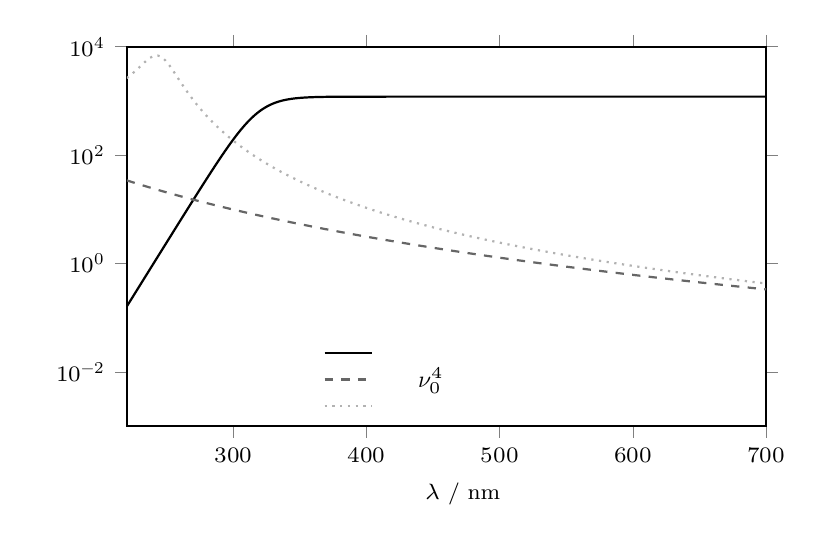
\begin{tikzpicture}
% declare function 必须放在 \begin{tikzpicture} 之后、\begin{axis} 之前，用 \tikzset 声明。
% 荧光背底用逻辑斯蒂函数（有界指数的形式，指数绝对值 < 80，不会触发 Dimension too large）。
\tikzset{declare function={
  fluor(\x) = 1200/(1+exp(-(\x-318)/11));
  rnr(\x)   = (532/\x)^4;
  rres(\x)  = (532/\x)^4*(1+300/(1+((\x-244)/14)^2));
}}
\begin{axis}[
  width=\onecolwidth, height=64mm,
  xmin=220, xmax=700, ymin=1e-3, ymax=1e4,
  ymode=log,
  xlabel={激发波长 $\lambda$ / nm},
  ylabel={相对信号强度（对数标度）},
  tick label style={font={\fontsize{8}{9.6}\selectfont}},
  label style={font={\fontsize{8}{9.6}\selectfont}},
  legend style={at={(0.30,0.02)}, anchor=south west, draw=none,
     fill=white, fill opacity=0.9, text opacity=1,
     font={\fontsize{8}{9.6}\selectfont}, row sep=0.5pt, inner sep=1.5pt},
  every axis plot/.append style={thick, no markers, samples=250, domain=220:700},
]
\addplot[black] {fluor(x)};
\addlegendentry{荧光背底（模型）}
\addplot[black!60, dashed] {rnr(x)};
\addlegendentry{非共振拉曼（$\nu_0^4$）}
\addplot[black!30, dotted] {rres(x)};
\addlegendentry{共振增强拉曼（模型）}
\end{axis}
\end{tikzpicture}
\caption{模型计算：同一物种在不同激发波长下的拉曼相对强度与荧光背底对比\modelmark。读者应看
三件事：（i）荧光背底（实线）在约 \qty{320}{nm} 以上迅速升到 $1.2\times10^3$ 并在整个可见区
保持平坦，因此可见激发的困难不是"峰弱"而是"背底高"；（ii）非共振拉曼（虚线）只按 $\nu_0^4$
变化，从 \qty{532}{nm} 换到 \qty{244}{nm} 只提高约 23 倍；（iii）共振增强拉曼（点线）在
\qty{244}{nm} 出现共振峰，把荧光/拉曼比压到约 $1:4.7\times10^3$，而 \qty{325}{nm} 处约
$11:1$、\qty{488}{nm} 处约 $4\times10^2:1$——这正是"488 nm 只有很强的荧光背景、325 nm 有干
扰但得到了谱图、244 nm 完全避开荧光"三条观测的定量对应。曲线为模型计算：荧光背底取中心
\qty{318}{nm}、宽 \qty{11}{nm} 的逻辑斯蒂函数，共振项取中心 \qty{244}{nm}、宽 \qty{14}{nm}
的洛伦兹因子（峰值增强 $3\times10^2$ 倍），$\nu_0^4$ 因子以 \qty{532}{nm} 归一；参数是为说明
机制设定的，不代表任何一种具体样品的真实数值，三条比值也不应当作定量判据使用。
\figsrc{机制与三条观测据 S1 §6.4.1、§6.4.6.2，书内 p.374、p.386 / PDF p.393、p.405}}
\label{fig:uv-fluor-model}
\end{figure}

\begin{table}[htbp]
\centering
\caption{三条激发波长路线的机制与代价。读者应看第三列：三条路线不是"哪个更好"，而是各自把不
同的一项当作代价付出去；选路线等于选愿意付哪一项。\src{据 S1 §6.4.1，书内 p.374 / PDF p.393；
§6.4.3，书内 p.377—378 / PDF p.396—397；§6.4.6，书内 p.382—384 / PDF p.401—403 归纳。}}
\label{tab:raman-routes}
{\srcsize
\begin{tabularx}{\columnwidth}{@{}lXX@{}}
\toprule
路线 & 避开荧光的机制 & 付出的代价与边界 \\
\midrule
可见（常见 \qty{532}{nm}、\qty{488}{nm}） & 不避开，只能靠扣基线、时间分辨或样品前处理抑制（见本章 §6.2 的四条路线） & 荧光常比拉曼强几个数量级，有时根本得不到光谱；深颜色样品在可见区吸收强，既有荧光又有激光加热 \\
近红外（FT-Raman，常见 \qty{1064}{nm}） & 近红外光频率低，一般不会激发电子吸收带，分子的荧光不被激发 & 散射强度按 $\nu_0^4$ 下降（$532\to1064$ 降到 $1/16$）；红外探测器灵敏度比可见区光电倍增管差至少两个数量级；样品热辐射干扰大；稀土与过渡金属离子的近红外跃迁仍会带来荧光；原位温度上限低（$<\qty{150}{\degC}$） \\
紫外（\qty{325}{nm}、\qty{257}{nm}、\qty{244}{nm}） & 分子被激发到高于第一电子激发态的虚态，虚态与第一电子激发态之间有间隙，荧光必须先无辐射放掉这一块能量，因此拉曼信号出现在比荧光波长更短的区域 & 紫外光源与紫外光路昂贵；深紫外下样品吸收强，探测深度变浅而成为表面灵敏技术；共振使峰高比不再等比；深色样品在紫外区是否仍强吸收需实测 \\
\bottomrule
\end{tabularx}}
\end{table}

\emph{核对说明}：已对照原页面图像（书内 p.374 / PDF p.393）。原书 §6.4.1
的两条路线与本表「机制」列一致：（1）「将激发波长向近红外（大于 \qty{700}{nm}）
方向移动可以避开大部分荧光，因为近红外光频率低，一般不会激发电子吸收带（图 6-17），
很多研究者通过采用傅氏变换拉曼光谱得到了没有荧光干扰的拉曼光谱」；（2）「将激发波长向深紫外（小于
\qty{300}{nm}）
方向移动……处于电子基态的分子被激发跃迁到一个高于第一电子激发态的虚态能级……由于在虚态能级和第一电子激发态之间有一个间隙，
所以拉曼信号出现在比荧光波长更短的区域，从而很有效地避开荧光干扰」。可见区一行「不避开荧光」
与原书「荧光干扰和灵敏度较差是阻碍常规拉曼光谱得到广泛应用的最大问题」的判断一致。各「代价」
列（$\nu_{0}^{4}$ 使 532 换到 1064 nm 后散射强度降到约 1/16、
红外探测器性能比可见区差约 2 个数量级、原位温度上限低于 \qty{150}{\degC}、
紫外光源与光学元件昂贵且样品吸收强等）出自 §6.4.3（书内 p.377—378 / PDF p.396—397）
与 §6.4.6（书内 p.382—384 / PDF p.401—403）。本轮重核（PDF p.396—397、
p.402—403 = 书内 p.377—378、p.383—384 页面图像）：近红外一行的五条代价在书内
p.378 逐条可查——$\nu_0^4$ 使灵敏度大幅降低、红外区检测器比可见区光电倍增管灵敏度至少
差两个数量级、热辐射干扰较大、稀土与过渡金属离子的近红外电子跃迁仍无法避开荧光、样品
温度上限低于 \qty{150}{\degC}；紫外一行的四条代价（光源与光路昂贵、探测深度变浅而表面
灵敏、共振使峰高比不再等比、深色样品需实测）在源书只正面列优势，未见对应表述，如实记为
改编。另：「\qty{257}{nm}」源书印 257.2 nm（514.5 nm 倍频），本表按其常用写法取整。


\subsubsection{紫外拉曼谱仪的四个特殊之处}

源文本给出的紫外拉曼光谱仪结构（图~\ref{fig:uv-fluor-model} 之外的仪器部分）与常规可见拉曼
仪有四处不同，每一处都对应紫外波段的一个物理限制\src{S1 §6.4.6，书内 p.383—384 /
PDF p.402—403}。

\textbf{（1）光源：靠倍频与气体激光器得到单线紫外。}光源采用腔内倍频氩离子激光器与
He—Cd 激光器：腔内倍频的紫外激光器是把氩离子激光器的可见激光经腔内 BBO 晶体倍频，得到多条
单线紫外激光，常用的有 \qty{514.5}{nm} 倍频所得的 \qty{257}{nm} 和 \qty{488}{nm} 倍频所得
的 \qty{244}{nm} 激光线；He—Cd 激光器可以提供 \qty{325}{nm} 的激光。

\textbf{（2）外光路：椭球收集镜解决两个问题。}外光路系统采用 180° 背向散射方式进行信
号采集，收集镜采用椭圆收集镜——它同时解决了"常规透镜在紫外区难以使用"和"随激发波长变化需
要重新调节焦距"两个问题；背向散射信号经紫外镀膜的椭球镜反射收集、会聚到光谱仪的入射狭缝
进入分光系统。

\textbf{（3）光谱仪：三光栅色散相减去掉瑞利线。}光谱仪采用三光栅结构，为适应紫外波段，光栅
和反射镜均采用紫外区镀膜。前两块光栅处于镜像对称位置，进行光谱的\textbf{色散相减}，其作用是
利于中间狭缝滤掉瑞利线；去除瑞利线后的散射光经第三块光栅 G3 分光后照射到 CCD 探测器。这也
解释了为什么这台仪器要用三块光栅而不是单光栅：\textbf{低波数能力是靠色散相减换来的}，代价是
多一次色散带来的光通量下降（与本章仪器部件表中"多联光谱仪光通量下降"是同一条折中）。

\textbf{（4）探测器：为紫外增强的液氮冷却 CCD。}液氮冷却 CCD 采用背向探测和紫外增强，使其在
紫外区进行信号检测的量子效率达到 $50\%$ 以上；液氮冷却使暗电流极低（$1$—$3$ 电子/(像元$\cdot$小
时)），可以瞬时快速地采集信号，采集速率可达毫秒级。进一步发展的紫外光谱仪采用三联光谱仪结
构，每联在线配置三块光栅，可在紫外区到可见区（$200$—\qty{700}{nm}）的较宽范围内进行拉曼光
谱研究，分辨率在紫外区为 \qty{2.0}{cm^{-1}}、在可见区为 \qty{1.0}{cm^{-1}}。国内第一台连续
波紫外共振拉曼光谱仪由中国科学院大连化学物理研究所于 1997 年建成。

关于最后那个分辨率差异，有一条容易漏掉的换算关系：\textbf{波数分辨率与波长分辨率之间差一个
$1/\lambda^2$}，即 $\delta\tilde\nu=\delta\lambda/\lambda^2$。同一个波长色散量在更短的波长下
对应更大的波数间隔，因此紫外区的"$\mathrm{cm^{-1}}$ 分辨率"必须单独标注，不能直接与可见区
的数值比较。

\subsubsection{读图实例：0.1 wt\% \ce{MoO3}/$\gamma$-\ce{Al2O3} 在三条激发线下的谱图}
\label{sec:ch06b-mo-instance}

这一小节把"换激发线"的全部判断链走一遍。样品是负载量 \num{0.1} wt\% 的
\ce{MoO3}/$\gamma$-\ce{Al2O3}，源文本给出了它的紫外可见漫反射谱与三条激发线（\qty{488}{nm}、
\qty{325}{nm}、\qty{244}{nm}）下的拉曼谱\src{S1 §6.4.6.2，书内 p.386 / PDF p.405}。下面的
两栏\textbf{严格分开}：观察栏只写谱图上直接可读的事实，推断栏只写由这些事实出发的归属与结论；
任何一句话不允许在两栏之间来回借用。

\begin{obs}
（观察——谱图上直接可读，不含任何归属）
\begin{itemize}
\item 紫外可见漫反射谱上主要出现两个吸收峰，分别位于 \qty{220}{nm} 与 \qty{280}{nm}。
\item \qty{488}{nm} 激发：谱图中没有得到任何拉曼信号，只有很强的荧光背底。
\item \qty{325}{nm} 激发：存在荧光干扰，但得到了拉曼光谱图。
\item \qty{244}{nm} 激发：完全避开了荧光干扰，得到信噪比很好的拉曼光谱图。
\item \qty{244}{nm} 谱中可读出：\qty{325}{cm^{-1}} 与 \qty{910}{cm^{-1}} 两个峰，以及
  \qty{1802}{cm^{-1}} 与 \qty{2720}{cm^{-1}} 两个峰。
\item \qty{325}{nm} 谱中可读出：\qty{837}{cm^{-1}} 处的峰及其 \qty{1670}{cm^{-1}} 的倍频峰。
\end{itemize}
\end{obs}

\begin{infer}
（推断——归属与结论，每一条都指回上面某一条观察）
\begin{itemize}
\item \qty{220}{nm} 的吸收峰归属于\textbf{四配位}钼物种的吸收，\qty{280}{nm} 的吸收峰主要归
  属于\textbf{六配位}钼物种的吸收。
\item \qty{244}{nm} 的激发线位于 Mo—O 键的荷电跃迁区，共振效应使 Mo—O 键对称伸缩振动模的
  \textbf{基频、倍频和三倍频}的谱峰强度\textbf{同时}发生增强，因此才得到了传统拉曼光谱无法得
  到的倍频与三倍频峰。
\item \qty{325}{nm} 的激发线位于 Mo—O—Mo 桥键的紫外吸收带，因此 \qty{325}{nm} 谱中
  \qty{837}{cm^{-1}} 的峰与其 \qty{1670}{cm^{-1}} 的倍频峰对应桥键物种的\textbf{反对称}伸缩振动。
\item 因此选用 \qty{244}{nm} 与 \qty{325}{nm} 两条激发线，可以分别有选择地增强"端基 Mo—O"
  与"桥键 Mo—O—Mo"，从而有效区分表面钼物种的配位结构。
\item 结论一：在极低负载量（\num{0.1} wt\%）时，四配位和六配位物种\textbf{同时存在}。这与过
  去高负载量催化剂的研究结果不同——以前推测认为在低负载量时只有四配位钼存在。
\item 结论二：由于紫外共振拉曼增强效应，极低负载量氧化物催化剂的研究成为可能。
\end{itemize}
\end{infer}

\textbf{为什么必须把两栏分开。}"\qty{488}{nm} 下没有拉曼信号"是观察；"因为荧光把拉曼淹没
了"是推断，它依赖图~\ref{fig:uv-fluor-model} 的模型（模型给出 \qty{488}{nm} 处荧光/拉曼比约
$4\times10^2$）与源文本"只有很强的荧光背景"的记述，而不是谱图本身能读出的东西。同理，
"\qty{244}{nm} 谱中有 \qty{1802}{cm^{-1}} 的峰"是观察；"它是 \qty{910}{cm^{-1}} 基频的二倍
频"是推断，需要先做归一性检查。把这两类句子分开写，是判断"这条结论有多大把握"的最省力办法
——读别人的谱图时也一样。

\emph{核对说明}：已对照原页面图像（书内 p.386 / PDF p.405）。原书印：\qty{244}{nm} 激光激发的
拉曼光谱中出现了归属为四配位 Mo=O 键的 \qty{325}{cm^{-1}} 和 \qty{910}{cm^{-1}} 的弯曲及对称
伸缩振动峰，以及在 \qty{1802}{cm^{-1}} 和 \qty{2720}{cm^{-1}} 归属为 Mo=O 键对称伸缩振动的
二倍频和三倍频峰；\qty{325}{nm} 激发谱中可观察到位于 \qty{837}{cm^{-1}} 和 \qty{1670}{cm^{-1}}
的六配位 Mo—O—Mo \textbf{反对称}伸缩振动的基频和倍频峰（原稿误作"对称"伸缩，已改）；漫反射谱
两吸收峰为 \qty{220}{nm}（四配位氧化钼）与 \qty{280}{nm}（六配位氧化钼）。原书的这些波数
\textbf{彼此不自洽}：$2\times910=1820\neq1802$、$3\times910=2730\neq2720$、$2\times837=1674
\neq1670$，属\textbf{原书自身问题}；本分片按原书\textbf{照录观测波数}，不代为换算基频（原稿曾据
$2\times901=1802$ 反推基频为 \qty{901}{cm^{-1}}，经读图证伪，已改回原书的 \qty{910}{cm^{-1}}）。

\begin{dataflow}
从"换一条激发线"到"这条峰属于哪种配位"的完整链条是：\textbf{换线 $\to$ 看哪些峰改变 $\to$
判断改变来自共振还是来自荧光/吸收 $\to$ 只对增强的那几条峰做归属 $\to$ 用第二条落在不同吸收
带的激发线交叉验证 $\to$ 才落到"某种配位物种存在"}。每一步都有失效方式：
\begin{itemize}
\item \textbf{峰强改变也可能来自样品本身的变化}：激光加热、吸水或脱水都会改变谱峰（见
  \S\,\ref{sec:ch06b-insitu}）。换线实验应在同一批样品、同一预处理下尽快完成，并记录两次测
  量之间的间隔与样品存放条件。
\item \textbf{倍频峰必须先做归一性检查}：$\tilde\nu_2\approx2\tilde\nu_1$、
  $\tilde\nu_3\approx3\tilde\nu_1$。本实例正是靠这条检查发现基频波数的 OCR 疑点；不做检查就
  可能把两个不同物种的基频当成同一物种的一组倍频。
\item \textbf{"某条激发线有共振"这一步需要吸收谱作依据}：没有该样品的紫外可见漫反射谱，就不
  能说 \qty{244}{nm} 落在哪一条吸收带上，"共振"只能算猜测。归属与吸收带的对应关系（如
  \qty{220}{nm} 对四配位）同样来自文献与参考谱，不是谱图自动给出的。
\end{itemize}
\end{dataflow}

\begin{table}[htbp]
\centering
\caption{三条激发线各自给出的观测与可用判断（本实例）。读者应看最后一列：每条线能回答的问题
是有限的，把三条线合起来才能把"端基/桥键/四配位/六配位"这组问题问完。\src{据 S1 §6.4.6.2，
书内 p.385—387 / PDF p.404—406 归纳；表中标注「模型」的荧光/拉曼比值为本改编本模型计算，
非源书实验数据。}}
\label{tab:mo-lines}
{\srcsize
\begin{tabularx}{\columnwidth}{@{}lXX@{}}
\toprule
激发线 & 源文本给出的观测 & 由这条线能得到的判断（含代价） \\
\midrule
\qty{488}{nm}（可见） & 没有任何拉曼信号，只有很强的荧光背底 & 判断：该样品的可见激发路线不可用，必须换线。代价：$\nu_0^4$ 因子最小、荧光背底最高（模型约 $7\times10^2$ 倍），此时"测不到"本身不能推出"没有该物种" \\
\qty{325}{nm}（近紫外） & 有荧光干扰但得到谱图；约 \qty{837}{cm^{-1}} 的峰及其倍频（倍频波数 OCR 丢失） & 判断：该线位于 Mo—O—Mo 桥键吸收带，\qty{837}{cm^{-1}} 可作为桥键物种的判据。代价：荧光仍占优（模型约 $11$ 倍），且只有与桥键电子跃迁耦合的模式被增强 \\
\qty{244}{nm}（深紫外） & 完全避开荧光，信噪比好；\qty{910}{cm^{-1}} 处基频，以及 \qty{1802}{cm^{-1}} 与 \qty{2720}{cm^{-1}} 的倍频、三倍频 & 判断：该线位于端基 Mo—O 荷电跃迁带，共振使基频/倍频/三倍频同时增强，可测到 \num{0.1} wt\% 级负载量。代价：峰高比不等于物种比；深紫外探测深度浅，读到的主要是表层 \\
\bottomrule
\end{tabularx}}
\end{table}

\subsubsection{紫外拉曼在催化中的五个落点}

紫外拉曼之所以在催化研究中具有很大的优势和潜力，源文本归结为三点：灵敏度高、避开荧光干扰，
以及"由于很多化合物的电子吸收带在紫外区，还可以进行共振拉曼光谱的研究"
\src{S1 §6.4.6，书内 p.384 / PDF p.403}。下面五个落点是源文本给出实例最多的方向，也是读者
最可能直接照用的方向。

\textbf{（1）催化剂积炭失活。}催化剂表面的积炭物种主要是一些高度脱氢的含碳化合物，如烯烃、
稠环芳烃、石墨前驱体和石墨；这些物种的形成机理和表面状态很难研究。虽然拉曼光谱在理论上应该
是一种理想的表征表面积炭的技术，但由于碳氢化合物有很强的荧光干扰，很难用可见拉曼光谱进行表
征。积炭的谱峰主要出现在三个区域：$1360$—\qty{1400}{cm^{-1}}（C—H 变形振动）、$1580$—\qty{1640}{cm^{-1}}
（C=C 伸缩）与 $2900$—\qty{3100}{cm^{-1}}（C—H 伸缩振动）；通过对这些谱峰的位置和相对强度的分析，可以区分烯烃、聚烯烃、芳烃、聚芳烃、类
石墨等不同形态的积炭。采用紫外激发线，不但使拉曼散射截面增加，而且有效避开荧光干扰，得到信
噪比很好的紫外拉曼光谱\src{S1 §6.4.6.1，书内 p.384 / PDF p.403}。

三种分子筛在甲醇转化反应中的积炭物种不同，这是"同类技术给出差异"的一个漂亮例子：
\begin{itemize}
\item \textbf{SAPO-34}：紫外拉曼谱中出现 1414、1616、1628、2822 与 \qty{2974}{cm^{-1}} 五个谱峰。
  其中 \qty{1414}{cm^{-1}} 谱峰为 \ce{CH3} 的变形振动，1616 与 \qty{1628}{cm^{-1}} 为烯烃的 C=C
  伸缩振动，2822 与 \qty{2974}{cm^{-1}} 为 C—H 键的对称与反对称伸缩振动——说明 SAPO-34 中形成
  的积炭物种主要是由\textbf{富含氢的烯烃和聚烯烃分子}组成。
\item \textbf{ZSM-5}：紫外拉曼谱中 \qty{1425}{cm^{-1}} 与 \qty{1615}{cm^{-1}} 的谱峰分别归属为
  芳烃和取代芳烃的 C—H 变形振动与 C=C 伸缩振动；在 ZSM-5 与 USY 的紫外拉曼谱图中\textbf{未检
  测到 C—H 振动区间的谱峰}。
\item \textbf{USY}：\qty{1604}{cm^{-1}} 谱峰为聚芳烃的 C=C 伸缩振动。
\end{itemize}
源文本的结论是：SAPO-34、ZSM-5 与 USY 三种分子筛在甲醇转化反应中形成了不同的积炭物种，这
是由它们不同的\textbf{酸性和孔结构}所决定的\src{S1 §6.4.6.1，书内 p.384—385 /
PDF p.403—404}。

\emph{核对说明}：已对照原页面图像（书内 p.384—385 / PDF p.403—404）。SAPO-34 的五个谱峰原书
印作 1414、1616、1628、2822 与 \qty{2974}{cm^{-1}}：\qty{1414}{cm^{-1}} 为 \ce{CH3} 的变形振
动，1616 与 \qty{1628}{cm^{-1}} 为烯烃的 C=C 伸缩振动，2822 与 \qty{2974}{cm^{-1}} 为 C—H 键
的对称与反对称伸缩振动；图 6-26 的 SAPO-34 曲线亦标注 2822 与 2974。原书归属句把后者印作
\qty{2947}{cm^{-1}}，与同页峰列表及图 6-26 标注不一致，属\textbf{原书自身问题}，本分片按峰列表
与图注取 2974。ZSM-5 与 USY 的归属亦据同页改正：ZSM-5 的 1425 与 \qty{1615}{cm^{-1}} 分别归属
为\textbf{芳烃和取代芳烃}的 C—H 变形振动与 C=C 伸缩振动（原稿误作"烯烃……C—C"），USY 的
\qty{1604}{cm^{-1}} 为聚芳烃的 C=C 伸缩振动（原稿漏数值）；"ZSM-5 与 USY 未检测到 C—H 振动区
间的谱峰"一句原书印于 SAPO-34 段末，本分片照录。积炭谱峰的三区间（$1360$—\qty{1400}{cm^{-1}}
C—H 变形、$1580$—\qty{1640}{cm^{-1}} C=C 伸缩、$2900$—\qty{3100}{cm^{-1}} C—H 伸缩）亦据同页
补正（原稿漏后两区间的数值）。

\textbf{（2）低负载量负载型过渡金属氧化物催化剂。}由于过渡金属氧化物在紫外区有荷电跃迁吸收，
选择合适的紫外激光进行共振激发，可以很有效地得到低负载量催化剂的紫外拉曼光谱。李灿等把紫外
拉曼用于低负载量 \ce{MoO3}/$\gamma$-\ce{Al2O3} 的研究，结果表明由于避开了荧光干扰、激发波长
变短和共振效应，信号灵敏度大幅度提高，甚至可以得到负载量低于 \num{0.1} wt\% 的
\ce{MoO3}/$\gamma$-\ce{Al2O3} 催化剂的谱图（即上一小节的读图实例）\src{S1 §6.4.6.2，书内
p.385—386 / PDF p.404—405}。

更重要的是这条路线能跟随\textbf{制备过程}：源文本报道用紫外拉曼研究负载型 \ce{MoO3} 催化剂
的制备与焙烧过程，结果表明在湿润状态时表面物种的配位结构不仅与浸渍液的 pH 有关，而且与载体
的性质有关；焙烧后几乎所有催化剂的表面钼物种都发生了变化，导致\textbf{四配位物种减少、六配
位物种增加}。作者用紫外拉曼灵敏地检测到负载钼物种随载体表面 pH 改变而发生的配位状态变化，
发现\textbf{表面 pH 是决定表面钼物种配位结构的重要因素}。由于绝大部分过渡金属氧化物在紫外区
有吸收，这项研究可以推广到其他氧化物\src{S1 §6.4.6.2，书内 p.387 / PDF p.406}。最后一句的方
法论含义值得单独记住：\textbf{紫外拉曼给出的不是"最终催化剂长什么样"，而是"制备条件如何一步
步写进表面配位结构"}。

\textbf{（3）原位跟踪分子筛的水热合成。}分子筛大多在高温高压的水热体系中合成，把中间产物取
出反应体系可能导致其结构性质发生明显变化；而原位表征可以在合成过程中测定中间物种，连续全面
地跟踪反应过程，得到最真实可靠的信息\src{S1 §6.4.6.3，书内 p.388 / PDF p.407}。拉曼在这里
有一个别人没有的条件：\textbf{水的拉曼散射截面非常小}，所以可以同时研究液相与固相信号；而合
成体系中通常存在大量富含模板剂的物种，它们产生极强的荧光，极大干扰常规拉曼测量——紫外拉曼
正好能避开这些中间物种的荧光干扰\src{S1 §6.4.6.3，书内 p.388 / PDF p.407}。原位池的做法见
\S\,\ref{sec:ch06b-insitu}。

X 型分子筛（\qty{373}{K}，水热条件）的两组观测构成了完整的机理证据链：
\begin{itemize}
\item \textbf{液相的观测}：最初的谱图有一个中心位于 \qty{500}{cm^{-1}} 的宽峰，以及位于 774
  与 \qty{920}{cm^{-1}} 的比较明显的谱峰。\qty{500}{cm^{-1}} 附近的谱峰归属于无定形硅铝凝
  胶前驱体；\qty{1060}{cm^{-1}} 的谱峰则是合成过程中碱性凝胶吸收空气中的 \ce{CO2} 产生的物
  种；774 与 \qty{920}{cm^{-1}} 被归属为液相中的\textbf{单态硅物种}。\qty{774}{cm^{-1}} 谱
  峰的强度随温度升高而逐渐加强，晶化到 \qty{120}{min} 时达到最大值，随后随反应时间延长逐渐
  下降——说明合成过程中存在大量单态硅物种，并且\textbf{单态硅物种参与了整个晶化过程}。
\item \textbf{由此描述的过程}：最初阶段无定形硅凝胶与液相中的物种处于平衡状态；随着反应温度
  提高，大量单态硅物种从硅凝胶前驱体当中解聚出来；随着反应进行，晶体的生长需要更多的单态硅
  物种；到晶化后期几乎所有无定形前驱体都被消耗并转变为晶形结构，不再解聚出单态硅物种。
\item \textbf{固相的观测}：初始凝胶处于无定形状态，给出位于 500、575、920 与 \qty{1060}{cm^{-1}}
  的谱峰。\qty{575}{cm^{-1}} 的谱峰在反应刚开始就存在，并且随着反应进行强度逐渐下降；当谱图
  中出现 298 与 \qty{380}{cm^{-1}} 的谱峰时，\qty{575}{cm^{-1}} 的峰基本消失——说明它代表合
  成中的一种\textbf{关键物种}。$550$—\qty{575}{cm^{-1}} 的谱峰被归属为 Al—O—Si 的伸缩振动；
  由于 \qty{575}{cm^{-1}} 与四元环呼吸振动的位置相差很远，它代表的 Al—O—Si 可能是以\textbf{支
  链}的形式存在，即来自位于四元环支链的 Al—O—Si 弯曲振动。
\item \textbf{晶化完成的判据}：随反应进行，固相 \qty{500}{cm^{-1}} 的谱峰移至
  \qty{514}{cm^{-1}}，后者归属于晶化完全的 X 型分子筛；同时对应于 X 型分子筛的特征峰
  \qty{298}{cm^{-1}} 与 \qty{380}{cm^{-1}} 强度增强，它们是由分子筛结构中\textbf{四元环和双
  六元环}的呼吸振动产生的。此外，固相中 \qty{774}{cm^{-1}} 与 \qty{920}{cm^{-1}} 谱峰的存
  在说明一部分单态硅物种吸附在固相表面或者是陷于固相中间。
\end{itemize}
综合原位拉曼、理论计算与 XRD、核磁共振谱，源文本给出 X 型分子筛合成机理的图景：无定形硅铝凝
胶不断解聚、溶解形成可溶性单态硅物种（\qty{774}{cm^{-1}}）；前驱体中存在四元环结构单元，其
中一些以支链形式存在（\qty{575}{cm^{-1}}）；四元环结构单元之间相互连接形成部分结晶的分子筛
结构（\qty{500}{cm^{-1}}）；晶化完全后该峰移至 \qty{514}{cm^{-1}}，并出现 \qty{298}{cm^{-1}}
与 \qty{380}{cm^{-1}} 的呼吸振动峰\src{S1 §6.4.6.3，书内 p.388—392 / PDF p.407—411}。

\textbf{（4）杂原子分子筛：共振选择性给出"杂原子是否进入骨架"的直接证据。}大部分分子筛催化
剂有较强的荧光干扰问题，原因之一是制备分子筛时残留的有机模板剂和合成原料中的杂质引起荧光；
因此在进行可见拉曼光谱表征前往往需要长时间的焙烧来消除荧光干扰，即使如此，很多分子筛的可见
拉曼光谱表征也是很困难的\src{S1 §6.4.6.4，书内 p.392 / PDF p.411}。三个实例：
\begin{itemize}
\item \textbf{TS-1}：以 \qty{244}{nm} 紫外激光作为激发光进行表征，通过紫外激光有选择性地激
  发了 TS-1 分子筛中 Ti—O—Si 之间的荷电跃迁，使与\textbf{骨架钛}直接相关的拉曼峰共振增强，
  得到钛进入骨架的最直接证据。TS-1 的紫外可见漫反射光谱在 \qty{220}{nm} 处有吸收峰，该峰归
  属于 Ti—O—Si 键骨架之间的 $\mathrm{p}\pi$—$\mathrm{d}\pi$ 荷电跃迁，而 Silicalite-1 在紫
  外区没有该吸收。与可见拉曼相比，紫外拉曼出现了 490、530 与 \qty{1125}{cm^{-1}} 三个新峰，
  这是骨架钛和骨架晶格氧原子之间的电荷跃迁受到紫外激光激发后产生的共振拉曼峰；由于共振效应，
  与骨架钛物种相关的拉曼谱峰增加了几个数量级。
\item \textbf{V-MCM-41}：紫外拉曼谱中 \qty{490}{cm^{-1}} 谱峰变宽，并在 930 与
  \qty{1070}{cm^{-1}} 出现两个新峰。\qty{930}{cm^{-1}} 的谱峰为\textbf{骨架外聚合}氧化钒的 V=O 对称伸缩振动峰，
  \qty{1070}{cm^{-1}} 的谱峰则为骨架四配位氧化钒的 V=O 对称伸缩振动峰。作者认为在可见拉曼光谱中未发现这两
  个峰，是由于 \qty{244}{nm} 波长的激发线\textbf{同时}激发了骨架钒和非骨架钒物种的荷电跃迁，
  共振效应使这两个峰的强度增强，从而同时得到了骨架钒与非骨架钒物种的谱峰。
\item \textbf{Fe-ZSM-5}（Si/Fe $=76$）：紫外可见漫反射谱最特征的吸收带位于 211 与
  \qty{245}{nm}，被归属为分子筛中骨架氧到骨架铁原子的荷电跃迁。三条激发线对比：\qty{244}{nm}
  位于该荷电跃迁吸收带、\qty{325}{nm} 处于它的吸收带边、\qty{532}{nm} 远离吸收带。\qty{244}{nm}
  谱中除 290、380 与 $800$ 附近的分子筛骨架特征峰以外，还激发出 516、1005、1115 与
  \qty{1165}{cm^{-1}} 四个新峰（这些峰在纯 ZSM-5 中是没有的）；\qty{325}{nm} 谱中这些峰仍
  在但强度弱了很多；\qty{532}{nm} 谱中只有 \qty{1005}{cm^{-1}} 的谱峰。作者把峰分为两类：
  \qty{1005}{cm^{-1}} 由铁的引入引起，但它是一个\textbf{非共振}峰；据对钛硅分子筛的归属，516 与
  \qty{1165}{cm^{-1}} 可归属为对称与反对称的 \ce{FeOSi} 四面体振动模式（原书未单独归属 1115）。此外，利用紫外拉曼还检测到了
  ZSM-5 分子筛中\textbf{痕量铁}的存在。
\end{itemize}
V-MCM-41 的例子里藏着一个重要提醒：\textbf{共振选择性的前提是"只有目标跃迁落在激发窗口内"}。
一旦两条跃迁（骨架钒与非骨架钒）落在同一波长窗口，选择性就消失——此时紫外拉曼把两类物种一起
增强，反而无法区分它们。

\emph{核对说明}：已对照原页面图像（书内 p.393—394 / PDF p.412—413）。图 6-35 题注为「Fe-ZSM-5
（Si/Fe $=76$）的（a）紫外可见漫反射谱图；（b）\qty{244}{nm}；（c）\qty{325}{nm} 和（d）
\qty{532}{nm} 激发的拉曼光谱图」。正文印：紫外可见吸收光谱图中最特征的吸收带位于
\textbf{\qty{211}{nm} 和 \qty{245}{nm}}，归为分子筛中骨架氧到骨架位铁原子的荷电跃迁；\qty{244}{nm}
谱中「除了位于 \qty{290}{cm^{-1}}、\qty{380}{cm^{-1}} 和 \qty{800}{cm^{-1}} 等分子筛骨架的特征峰
以外」还激发出 516、1005、1115 与 \qty{1165}{cm^{-1}} 四个新峰（原稿「$800$ 附近」已按原书改为
精确值）；\qty{325}{nm} 谱中 \qty{1005}{cm^{-1}} 仍见而 516/1115/1165 强度弱了很多；\qty{532}{nm}
谱中只有 \qty{1005}{cm^{-1}}。峰的两类划分亦据原书：\qty{1005}{cm^{-1}} 由铁的引入引起但是
\textbf{非共振}峰，「根据对钛硅分子筛的归属，\qty{516}{cm^{-1}} 和 \qty{1165}{cm^{-1}} 可以归属为
对称和反对称的 \ce{FeOSi} 四面体的振动模式」——\qty{1115}{cm^{-1}} 原书\textbf{未单独归属}，本分片
不再把它列入四面体振动模式。

\textbf{（5）氧化物表面相变：紫外拉曼为什么比 XRD 更"表面"。}这是本节方法论价值最高的一段，
它把"信息深度"从一个抽象概念变成了可验证的读数差异。

\textbf{判据的物理基础}：一般来讲，拉曼散射信号是同时来自样品体相和表面的；但当样品对激发
和散射光有很强吸收时，来自体相的信号会很大程度地衰减，拉曼谱图反映的主要是\textbf{样品表面
区}的信息。大多数过渡金属氧化物对紫外光有很强的吸收，因而紫外拉曼光谱对这些样品的表面信息
比体相信息更为灵敏；而大多数样品在可见区都没有吸收，因此可见拉曼光谱给出的是\textbf{体相和
表面二者混合}的信息\src{S1 §6.4.6.5，书内 p.395 / PDF p.414}。

\begin{itemize}
\item \textbf{\ce{ZrO2}：表面先相变。}紫外拉曼谱显示：\qty{400}{\degC} 焙烧后可以观察到四方
  和单斜混合相的拉曼谱峰；\qty{500}{\degC} 焙烧后四方相谱峰完全消失，仅有单斜相的谱峰被观察
  到；升温到 \qty{700}{\degC}，单斜相谱峰进一步增强。但 XRD 图谱显示 \qty{400}{\degC} 焙烧
  后氧化锆主要以\textbf{四方相}结构存在，甚至焙烧样品在 \qty{700}{\degC} 后仍然能观察到四方
  相的存在；可见拉曼与 XRD 的结果非常相似，而与紫外拉曼的结果却明显不同。作者的结论是：氧化
  锆的相变是一个从表面到体相的过程，即\textbf{单斜相首先在四方相晶粒的表面形成}；尽管单斜相
  是热力学更稳定的相，但由于动力学的原因，从四方相到单斜相的相变需要一个缓慢的从表面到体相
  的过程。
\item \textbf{掺杂 \ce{ZrO2}：体相稳定不等于表面稳定。}从紫外拉曼、XRD 和可见拉曼的结果看，
  尽管由于稳定剂的加入，四方相能稳定存在于样品体相，但\textbf{四方相在表面仍不能被稳定}，
  极易转变为单斜相；特别是当稳定剂含量低时，样品表面完全处于单斜相结构；稳定剂在样品表面含
  量足够高时，样品可完全稳定在四方相。
\item \textbf{\ce{TiO2}：表面后相变，方向与 \ce{ZrO2} 相反。}XRD 与可见拉曼给出的是体相信
  息：焙烧温度达到 \qty{550}{\degC} 时，除锐钛矿的特征衍射峰之外还在 $27.6$°、$36.1$°、
  $41.2$° 和 $54.3$° 出现金红石的特征衍射峰，表明此时发生了从锐钛矿到金红石的相变；可见拉曼
  在 \qty{550}{\degC} 观察到很弱的金红石特征峰（\qty{445}{cm^{-1}}），\qty{580}{\degC} 之后
  又观察到金红石的另外两个特征峰 \qty{235}{cm^{-1}} 和 \qty{612}{cm^{-1}}；温度达到
  \qty{750}{\degC} 时锐钛矿的特征峰完全消失，相变完成。紫外拉曼给出的表面信息不同：样品在
  \qty{500}{\degC} 焙烧后可以明显观察到锐钛矿的特征峰（143、395、\qty{515}{cm^{-1}}），直到
  温度升高到 \qty{700}{\degC} 才能在紫外拉曼光谱上观察到金红石的特征峰（\qty{235}{cm^{-1}}）。
  因此\textbf{表面上锐钛矿的相变要滞后一些}，作者认为氧化钛的相变是从\textbf{团聚粒子的体相
  开始、逐渐发展到表面区域}的。
\item \textbf{把表面晶相接到催化活性上。}采用光催化分解水作为指标反应，考察不同温度焙烧的氧
  化钛催化剂的产氢活性：只要表面处于锐钛矿相（焙烧温度 $<\qty{680}{\degC}$），即使体相的锐钛
  矿—金红石含量有很大差别，样品的产氢活性基本没有明显变化；\qty{700}{\degC} 和
  \qty{750}{\degC} 焙烧之后光催化活性有所提高——这两个样品的体相中基本上均处于单一金红石晶
  相，但\textbf{表面处于锐钛矿和金红石的混合晶相}；焙烧温度升高到 \qty{800}{\degC} 时表面完全
  处于金红石晶相，产氢活性急剧降低。作者认为表面锐钛矿—金红石的\textbf{异相结}有利于电子—
  空穴分离，从而提高光催化活性。为验证这一结论，他们用浸渍并焙烧的方法制备了金红石负载的锐
  钛矿样品 \ce{TiO2(A)/TiO2(R)}-$n$（$n$ 为浸渍次数）：浸渍次数从 1 增加到 4 次时，用紫外拉
  曼的估算结果表明表面锐钛矿含量从 $10\%$ 增加到 $36\%$；\ce{TiO2(A)/TiO2(R)}-3 样品的光催
  化活性基本上是纯金红石载体的 4 倍，而未经过焙烧的样品活性非常低（甚至比金红石载体还低，可
  能因为金红石表面上覆盖了一层无定形 \ce{TiO2}）。上述结果说明：\textbf{相比于体相晶相，光催
  化活性更多地取决于表面区的晶相}。
\item \textbf{钼酸铁：表面富集。}\ce{Fe2(MoO4)3} 也是一类在紫外区有强吸收的材料。可见拉曼谱
  随焙烧温度升高，\ce{Fe2(MoO4)3} 与 \ce{MoO3} 的特征峰相对强度变化不大；紫外拉曼谱则表明随
  焙烧温度升高 \ce{MoO3} 的特征峰强度不断增加，\qty{700}{\degC} 焙烧后主要显示为 \ce{MoO3}
  的特征峰——说明随焙烧温度升高 \ce{MoO3} 逐步\textbf{在表面富集}。扫描电镜的结果支持这一判
  断：\qty{500}{\degC} 焙烧的样品主要为球形颗粒的聚集体，\qty{700}{\degC} 焙烧后除颗粒长大
  外还可明显观察到棒状物种出现；文献一般认为这种形貌为 \ce{MoO3} 的特征形貌，而且 EDX 结果
  也表明棒状区域为富钼区域。
\end{itemize}
源文本对这一段的总评是：紫外拉曼不仅对研究如氧化锆、氧化钛及钼酸铁等系列在紫外区有强吸收的
材料的表面相变及表面相组成具有优势，而且对研究半导体材料的光催化性能具有很大的优势
\src{S1 §6.4.6.5，书内 p.396—402 / PDF p.415—421}。

\begin{table}[htbp]
\centering
\caption{紫外拉曼在催化中的五个落点：关键谱峰与"为什么必须用紫外"。读者应看最后一列——每个
落点都需要紫外，但需要的\textbf{理由并不相同}：前四个靠"避开荧光 $+$ 共振选择性"，第五个靠
"强吸收导致的表面灵敏"。\src{据 S1 §6.4.6.1—§6.4.6.5，书内 p.384—402 / PDF p.403—421 归纳。}}
\label{tab:uv-apps}
{\srcsize
\begin{tabularx}{\columnwidth}{@{}lXX@{}}
\toprule
应用对象 & 紫外拉曼给出的关键谱峰 & 为什么必须用紫外 \\
\midrule
分子筛积炭（SAPO-34、ZSM-5、USY） & 积炭总体在 $1360$—\qty{1400}{cm^{-1}}；SAPO-34：1414、1616、1628、2822、2974；ZSM-5：1425、1615；USY：1604（聚芳烃 C=C 伸缩） & 碳氢化合物荧光极强，可见拉曼很难表征；紫外激发同时提高散射截面并避开荧光 \\
低负载量 \ce{MoO3}/$\gamma$-\ce{Al2O3}（\num{0.1} wt\%） & \qty{244}{nm}：910、1802、2720；\qty{325}{nm}：837 及倍频 & 激发线落在 Mo—O 与 Mo—O—Mo 的荷电跃迁带内，共振使信号增强数个数量级；可见激发只剩荧光 \\
X 型分子筛水热合成（原位） & 液相：500、774、920、1060；固相：500（晶化后移至 514）、575、298、380 & 合成体系含大量有机模板剂，荧光极强；水的拉曼截面很小，故可同时测液相与固相 \\
杂原子分子筛（TS-1、V-MCM-41、Fe-ZSM-5） & TS-1：490、530、1125；V-MCM-41：930、1070；Fe-ZSM-5：516、1005、1115、1165 & 需要\textbf{选择性}共振激发杂原子—氧的荷电跃迁，从而只增强与骨架杂原子相关的模式 \\
氧化物表面相变与表面组成（\ce{ZrO2}、\ce{TiO2}、\ce{Fe2(MoO4)3}） & \ce{TiO2} 锐钛矿 143、395、515 / 金红石 235、445、612；\ce{ZrO2} 四方与单斜各自的谱峰 & 紫外强吸收把体相信号衰减掉，信号主要来自表面区，从而把\textbf{表面相}与\textbf{体相}分开 \\
\bottomrule
\end{tabularx}}
\end{table}

\emph{核对说明}：本表第一行「分子筛积炭」已对照原页面图像（书内 p.384—385 / PDF p.403—404），
原书 SAPO-34 的谱峰为 1414、1616、1628、2822 与 \qty{2974}{cm^{-1}}，ZSM-5 为 1425 与
\qty{1615}{cm^{-1}}，USY 为 \qty{1604}{cm^{-1}}（聚芳烃的 C=C 伸缩振动）；本表原印 2947 与
「C—C 伸缩」均与原文不符，已改正。本轮重核其余四行（PDF p.405、p.409、p.411、p.415 = 书内 p.386、p.390、p.392、p.396 页面图像）：
低负载 \ce{MoO3}/$\gamma$-\ce{Al2O3} 一行与书内 p.386 的 244 nm（325、910、1802、\qty{2720}{cm^{-1}}）
与 325 nm（\qty{837}{cm^{-1}} 及倍频）两组波数一致；X 型分子筛一行与书内 p.390 的液相
500、774、920、\qty{1060}{cm^{-1}} 与固相 500（晶化后移至 514）、575（肩峰）、298、
\qty{380}{cm^{-1}} 逐项一致；杂原子分子筛一行 TS-1 的 490、530、\qty{1125}{cm^{-1}} 与
p.392 逐字一致（V-MCM-41 与 Fe-ZSM-5 两组在同节后页，未逐字对读，本表如实标为差异）；
氧化物表面相变一行的「自吸收使信号只来自表面」机制与 p.396 逐字一致，锐钛矿/金红石的六个
峰位未在所读页面出现，如实标为差异。另记源书自身的一处不一致：X 型分子筛的固相峰在 p.390
正文作 298、在 p.392 图 6-33(b) 标注作 290，本表按正文取 298。

\subsection{表面增强拉曼与共焦拉曼}

\subsubsection{SERS 的两种增强机制}

自 1974 年 Fleischmann 等首次从吸附物种的拉曼光谱中发现表面增强拉曼散射
（Surface-Enhanced Raman Scattering，SERS）以来，这方面工作发展非常迅速，理论和实验研究均
有大量报道，目前已成为拉曼光谱中一个非常活跃的领域\src{S1 §6.4.4，书内 p.378 / PDF p.397}。
SERS 的价值在于它把"极弱"的拉曼散射放大到可以测单层吸附物种的程度——这正是催化表面研究最
想要的能力。

\begin{principle}
\textbf{两种机制，对应诱导偶极公式的两个因子。}关于 SERS 的机理基本上有两种观点，把
$P=\alpha E$ 写开就一目了然：

\begin{equation}
P \;=\; \alpha\,E:\qquad
\text{电磁机制使 } E \text{ 增大},\qquad
\text{化学机制使 } \alpha \text{ 增大}
\label{eq:sers-two}
\end{equation}

\textbf{电磁机制}（物理增强为主）：认为 SERS 起源于激发光和拉曼散射光被粗糙的金属表面局部
电场增强，即 $P=\alpha E$ 中的 $E$ 增大。\textbf{化学机制}（化学吸附为主）：认为增强来自吸
附分子与金属之间的电荷转移而引起的分子极化率增加，即 $P=\alpha E$ 中的 $\alpha$ 增大。

\textbf{两种机制对定量的含义完全不同}：电磁增强几乎不挑分子种类（挑的是分子离金属表面的距
离与取向，以及它是否落在局域电场增强区里），因此它对同一分子内不同振动模式的影响相对温和，
但随位置剧烈变化；化学增强只出现在能形成特定吸附键与电荷转移共振条件的分子—金属组合上，并
会\textbf{改变相对峰高}。真实体系的净增强同时含有两个贡献，无法用一组标定把它们分开
\src{S1 §6.4.4，书内 p.378 / PDF p.397}。
\end{principle}

能产生 SERS 效应的金属很多，如 Ag、Au、Cu、Fe、Co、Ni、Al 等，常用的是 Ag、Au 和 Cu；获得
活性金属表面的方法有溶胶化学还原法、真空蒸馏法与化学沉积法\src{S1 §6.4.4，书内 p.378 /
PDF p.397}。源文本也直接给出了这条技术的边界：利用 SERS 研究\textbf{所有的金属和金属氧化物}
表面增强是不可能的，研究最多的是 Ag、Au 和 Cu；在这三种常用基质上可以进行有机分子、
\ce{SO2}、\ce{NO2}、\ce{CO}、\ce{NH3} 等物质的吸附和反应研究\src{S1 §6.4.4，书内 p.378 /
PDF p.397}。

三个有代表性的实验事实：
\begin{itemize}
\item \textbf{共吸附会改变基底。}有作者用 SERS 研究多孔 Ag 薄膜，观察到了 \ce{N2} 和 \ce{CO}
  增强的拉曼谱带，但 \ce{O2} 的拉曼谱带并没有被明显增强；若在吸附吡啶和乙烯以前，先在 Ag 表
  面吸附少量 \ce{O2}，吡啶和乙烯吸附物种的增强谱带会很大衰减。作者认为这可能是 \ce{O2} 的存
  在减少了其他分子在表面的吸附浓度、引起了其他分子的解离、改变了表面形态。注意作者只给出
  "可能"的解释——这本身就是一条读法提示：\textbf{预吸附改变了基底本身}，此后任何强度比较都不
  再可比。
  \item \textbf{增强因子的量级。}Feilchenfeld 和 Siiman 研究了 \ce{CrO4^{2-}} 在 Ag 溶胶
  中吸附的 SERS，其中 \textbf{Cr—O 键}的伸缩振动模式最大增强接近 $\num{1.1e5}$，此时激发
  光波长为 \qty{580.0}{nm}
  \src{S1 §6.4.4，书内 p.378—379 / PDF p.397—398}。
\item \textbf{电位依赖的 C—O 伸缩频率。}Tadayyoni 和 Weaver 报道了 \ce{HClO4} 溶液中 CO 的
  SERS：C—O 伸缩振动频率随电极上电压的改变在 $2080$—\qty{2110}{cm^{-1}} 之间变化；\textbf{不加
  电压}时，C—O 振动频率位于 \qty{2015}{cm^{-1}}——这与 CO 在催化剂表面的吸附频率完全一致。
  SERS 真正的强项：它测的是\textbf{吸附态的键与取向}，而且可以在电化学条件下原位测。
\end{itemize}

\emph{核对说明}：已对照原页面图像（书内 p.378—379 / PDF p.397—398）。原书印「Cr—O 键伸缩振动
模式最大增强接近 $1.1\times10^{5}$，此时激发光波长为 \qty{580.0}{nm}」——原稿因 OCR 损坏
（作「ｃ卜。键伸缩振动」）只写作"某一键的伸缩振动模式"，现按原书补出\textbf{Cr—O 键}。该例为
Feilchenfeld 和 Siiman$^{[165]}$ 研究 \ce{CrO4^{2-}} 在 Ag 溶胶中吸附的 SERS，图 6-21 为吸附的
\ce{CrO4^{2-}} 随激发光频率变化的表面增强拉曼光谱（激发波长 457.9、488.0、514.5、593.1、607.2、
676.4 nm，图上另标 \qty{796}{cm^{-1}} 的 \ce{CrO4^{2-}} on Ag 与 \qty{1020}{cm^{-1}} 的
\ce{CH3OH}）。C—O 一例原书印「Tadayyani 和 Weaver$^{[166]}$ 报道了在 \ce{HClO4} 溶液存在下 Au
电极上 CO 吸附的 SERS。C—O 伸缩振动频率随电极上电压的改变在 $2080\sim2110\,\mathrm{cm^{-1}}$
之间变化。\textbf{没有电压时}，C—O 振动频率在 \qty{2015}{cm^{-1}}，这与 CO 在催化剂表面的吸附
频率是完全一致的」——原稿误作"某一电压下"，已改为"不加电压时"；第二个姓原书自身印作
\textbf{Tadayyani}，本分片按通行文献拼写取 Tadayyoni。

\subsubsection{SERS 为什么不给浓度}
\label{sec:ch06b-sers-quant}

\begin{pitfall}
\textbf{把 SERS 的峰强度直接当作浓度}，是这项技术最典型、也最容易被"极高灵敏度"这句话诱导
出来的误判。三条理由互相独立，任何一条都足以推翻定量结论。

\textbf{（1）热点分布决定强度，而热点是纳米尺度的。}电磁增强来自粗糙金属表面（颗粒间隙、
尖端、聚集体缝隙）的局域电场增强，有效区域只占表面的很小一部分。分子落在热点里与落在热点外，
增强因子可以相差若干数量级，因此谱峰强度反映的是"\textbf{分子恰好位于热点中的概率} $\times$
表面浓度"，而前者随基底形貌、颗粒尺寸乃至分子自身大小变化。把强度当作浓度的直接读数，等于
假设热点分布对所有样品相同。

\textbf{（2）吸附取向改变相对峰高。}式~\eqref{eq:sers-two} 中的 $\alpha$ 是张量，SERS 强度
取决于分子某一振动模式的极化率张量分量与表面局域电场方向的匹配。同一个分子以不同取向吸附时，
不同振动模式的增强因子不同，所以\textbf{不仅绝对强度不可比，峰高比也不可比}；比较两个样品的
同一峰高比，等于默认两者的取向分布相同——而这个默认在催化体系里通常不成立（表面覆盖度、共吸
附物种、电位都会改变取向）。

\textbf{（3）基底不可复现。}获得活性表面的方法是溶胶化学还原、真空蒸馏与化学沉积，得到的颗
粒尺寸、间隙分布与表面粗糙度难以逐批重现，增强因子因此在批次间漂移。源文本给出的限制更硬：
能产生 SERS 信号的金属和金属氧化物是有限的，研究最多的是 Ag、Au 和 Cu；而且由于在 SERS 研
究中对样品的制备技术要求很高，\textbf{对实际催化剂来说是不容易实现的}，这些使得 SERS 在催化
研究中的进一步应用受到了限制\src{S1 §6.4.4，书内 p.379 / PDF p.398}。

\textbf{要定量只有三条路，且都必须写进图注}：加入内标并测内标峰与目标峰的强度比；在同一种基
底、同一批次上做浓度标定曲线（并给出线性范围）；在同一基底上统计多个点，把热点分布平均掉。
三条都不做，SERS 谱只能回答"有什么物种、以什么取向吸附"，不能回答"有多少"。
\end{pitfall}

\subsubsection{共焦拉曼：剖层分析能剖到多薄}
\label{sec:ch06b-confocal}

共聚焦技术的原理早在 1957 年就已提出，并于 1967 年被用于光学切片分析；1977 年，该技术首次用
于拉曼光谱学\src{S1 §6.4.5，书内 p.379 / PDF p.398}。

\textbf{光路与剖层。}共焦拉曼显微镜的工作原理是：针孔 H1 把激光聚焦于样品表面，样品表面的
被照射点在探测针孔 H2 处成像，其信号由 H2 后的检测器收集；而当激光在样品表面是散焦时，样品
处的大部分信号被 H2 挡住，无法通过针孔到达检测器。把样品沿着激光入射方向上下移动，就可以把
激光聚焦于样品的不同深度，这样所采集的信号也将来自样品的不同深度，实现\textbf{样品的剖层分
析}。这种结构的最大特点就是可以有效地\textbf{排除来自聚焦平面之外其他层信号的干扰}；显微镜
头的数值孔径越大、探测针孔的直径越小，仪器的共焦性能就越好\src{S1 §6.4.5，书内 p.379—380 /
PDF p.398—399}。

\textbf{共焦拉曼的优点}：①高灵敏度，可用于弱拉曼信号的测量；②共聚焦技术的使用使显微镜下激
光在样品上的焦点准确地通过针孔，从而很大程度地提高了\textbf{纵向空间分辨率}，可研究直径为
$1\,$µm 的样品，用于原位多层材料测量；同时共焦显微系统本身还具有较高\textbf{水平方向}的空
间分辨率，而这一分辨率仅取决于显微镜头的放大倍数和所用的激光波长\src{S1 §6.4.5，书内
p.380 / PDF p.399}。

图~\ref{fig:confocal-axial} 用一个模型计算说明"共焦能剖多薄"以及它在什么情况下会失效。

\begin{figure}[tbp]
\centering
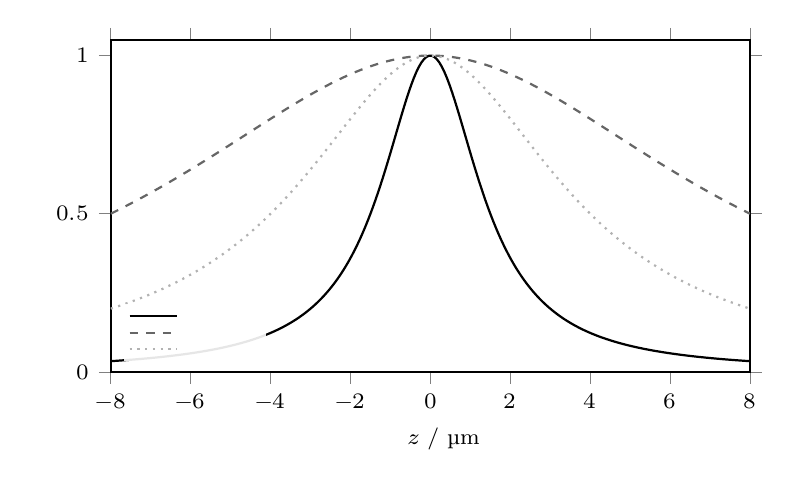
\begin{tikzpicture}
\tikzset{declare function={
  nohole(\x) = 1/(1+(\x/8)^2);
  confoc(\x) = 1/(1+(\x/1.5)^2);
  broad(\x)  = 1/(1+(\x/4)^2);
}}
\begin{axis}[
  width=\onecolwidth, height=58mm,
  xmin=-8, xmax=8, ymin=0, ymax=1.05,
  xlabel={离焦量 $z$ / µm},
  ylabel={归一化收集效率},
  xtick={-8,-6,-4,-2,0,2,4,6,8},
  tick label style={font={\fontsize{8}{9.6}\selectfont}},
  label style={font={\fontsize{8}{9.6}\selectfont}},
  legend style={at={(0.02,0.03)}, anchor=south west, draw=none,
     fill=white, fill opacity=0.9, text opacity=1,
     font={\fontsize{8}{9.6}\selectfont}, row sep=0.5pt, inner sep=1.5pt},
  every axis plot/.append style={thick, no markers, samples=250, domain=-8:8},
]
\addplot[black] {confoc(x)};
\addlegendentry{有针孔（理想共焦）}
\addplot[black!60, dashed] {nohole(x)};
\addlegendentry{无针孔（常规显微）}
\addplot[black!30, dotted] {broad(x)};
\addlegendentry{折射率失配或强散射介质}
\end{axis}
\end{tikzpicture}
\caption{模型计算：共焦针孔对轴向（深度）响应的影响\modelmark。读者应看三件事：（i）无针孔时
（虚线）离焦 $\pm5\,$µm 仍收到大部分信号，深度选择性很弱；（ii）加针孔后（实线）只保留焦平
面附近很薄一层的信号，这就是"剖层分析"能成立的物理原因，也是它能测 $1\,$µm 级样品的依据；
（iii）当焦深因样品折射率与物镜标称介质不同、或样品强散射使焦点展宽时（点线），同一针孔的轴
向响应被显著拉宽，深度标度也不再是位移台读数的线性函数——此时"某物种只出现在距表面 $d$ 处"
的结论必须附深度标定数据。三条曲线为洛伦兹型轴向响应的模型计算，半高宽分别取 $16\,$µm、
$3\,$µm 与 $8\,$µm（即参数 $8$、$1.5$、$4$），不代表任何一台仪器或任何一个样品的实测响应；
图例置于左下角并以白底覆盖的仅是三条曲线的尾部（左半支与右半支镜像，形状可由右半支读出）。
\figsrc{剖层原理据 S1 §6.4.5，书内 p.379—380 / PDF p.398—399}}
\label{fig:confocal-axial}
\end{figure}

\textbf{两个应用实例。}

\textbf{（1）混合氧化物催化剂的空间不均一性。}\ce{SEM}-\ce{EDX}（扫描电镜—能量弥散 X 射线）
成像表明 Mo、V 和 W 混合氧化物催化剂中几种元素分布是不均一的；而该催化剂的 XRD 仅给出无定形
相的衍射峰，拟合后表明可能有两种物相存在（无定形 \ce{MoO3} 和无定形 \ce{Mo5O14}）。作者用共
焦拉曼在 $30\times30\,$µm 的催化剂区域内获得了 1000 个拉曼光谱，并用化学计量学方法从 1000 个
光谱中解析出两个主要组分的光谱：组分 1 可能是主要含有 Mo 和 W 的缺氧 \ce{MoWO_{3-x}} 结构，
组分 2 则表明可能是无定形 \ce{V2O5} 的贡献。综合其他分析方法的结果，作者认为在铝基混合氧化
物催化剂中，缺氧的 \ce{MoWO_{3-x}} 组分优先在\textbf{小的高 V 样品区域内}形成，而
\ce{V2O5} 型氧化物是在具有 Mo 和 W 均匀分布的\textbf{剩余区域内}形成的
\src{S1 §6.4.5，书内 p.380—381 / PDF p.399—400}。这个实例的方法论价值在于：\textbf{XRD 给出
的是整块样品的平均物相，共焦拉曼给出的是物相的空间分布}，两者互补而不互相替代——单点 XRD 永
远无法告诉你"哪个组分在哪个微区里"。

\textbf{（2）电极界面的浓度梯度。}田中群等用共焦拉曼显微技术研究了在电催化和燃料电池中有重
要意义的甲醇氧化过程。利用共焦显微拉曼可以剖层分析的特点，他们把激光聚焦于电极表面时，拉曼
信号主要来自电极表面吸附物种；而把激光聚焦在电极表面之上时，拉曼信号则主要来自体相溶液。因
而通过改变激光聚焦点与电极表面的距离，他们得到了反应过程中各物种随离电极表面距离 $d$ 变化的
\textbf{浓度梯度关系}。实验中不仅检测到该体系发生解离吸附的中间产物（CO），还同时监测到溶液
成分的变化——他们的研究表明共焦拉曼光谱可以作为一种多功能的界面研究和分析技术
\src{S1 §6.4.5，书内 p.381—382 / PDF p.400—401}。

\textbf{代价同样存在。}源文本明确指出：由于共焦技术的使用，在一定程度上会破坏样品，并且使原
位检测催化反应变得困难\src{S1 §6.4.5，书内 p.382 / PDF p.401}。这两条限制分别对应高数值孔径
物镜必须在极近距离工作（工作距离短、功率密度高、样品池设计受限），以及共焦光路对窗口与针孔
对准的苛刻要求。

\begin{pitfall}
\textbf{把共焦图上的空间分辨当成物镜的标称分辨。}共焦拉曼的深度选择性由三样东西共同决定，
而它们都不写在"放大倍数"里：
\begin{itemize}
\item \textbf{折射率。}物镜的焦深与横向分辨是按空气（$n\approx1$）标定的；在液相中测量、或
  隔着窗口测样品时，实际焦点位置与标称深度不成正比——介质折射率与物镜设计值不匹配会引入球差，
  使焦点展宽并让深度标度非线性（图~\ref{fig:confocal-axial} 的点线）。用共焦做"浓度随深度
  $d$ 变化"的定量时，\textbf{深度尺度必须用已知标样标定}，不能拿位移台的读数当深度。
\item \textbf{散射体积与多次散射。}针孔只能挡住"离焦"的光，挡不住"在别处被散射之后又拐进针
  孔"的光。催化剂粉末、凝胶与多孔载体都是强散射介质，此时有效采样体积远大于理想共焦体积，横
  向分辨也随之恶化。上文两个实例之所以成立，一个是因为样品是相对致密的氧化物颗粒聚集体，一个
  是因为界面附近的溶液是弱散射介质。
\item \textbf{波长与功率密度。}横向空间分辨率取决于物镜放大倍数与激光波长，紫外激发能给出更
  小的衍射极限，但深紫外物镜的数值孔径与工作距离往往更差；共焦小体积内的功率密度更高，于是又
  回到 \S\,\ref{sec:ch06b-insitu} 的激光加热问题——源文本所说的"共焦技术的使用在一定程度上会
  破坏样品"，正是这一条的实验表现。
\end{itemize}
因此报告共焦结论时必须给出四个参数：\textbf{物镜数值孔径、针孔直径、步长、激发波长与样品介
质}。缺任何一项，别人都无法复现"这个物种出现在哪个深度"。
\end{pitfall}

\subsubsection{应用部分四条误判的汇总}

\begin{pitfall}
本章应用部分最容易犯的四条误判，放在一起对照。它们的共同结构是：\textbf{强度与位置的变化都
存在"非结构"的解释通道}，而排除这些通道只需要改变一个可写进图注的条件。

\begin{itemize}
\item \textbf{把激光加热导致的谱带位移当结构变化。}排除办法是改变激光功率重测并检查时间依赖
  与可逆性（三条判据见 \S\,\ref{sec:ch06b-insitu}）。
\item \textbf{把荧光背底当成宽峰。}宽荧光背景在扣基线之后常留下一个"包"，很容易被当成无定形
  物种或聚合物种的宽峰——分子筛与积炭样品尤其危险，因为模板剂、杂质与碳氢物种都产生极强荧光。
  两条判据：换激发波长重测，真拉曼峰的位移不动、而荧光包的位置随激发波长大幅移动（"峰按位移
  标定、荧光按波长标定"，见本章 §6.2 的"数据到结论"一栏）；测空样品池与纯载体，看这个包是否
  来自样品本身。此外，扣基线方式会直接改变弱峰的相对强度，凡做定量比较必须声明扣基线方法。
\item \textbf{把 SERS 强度直接当浓度。}热点分布、吸附取向与基底批次三者共同决定强度，且能产
  生 SERS 的金属与金属氧化物有限（见 \S\,\ref{sec:ch06b-sers-quant}）。
\item \textbf{把共焦的标称分辨当成实际分辨。}折射率与散射体积都会拉宽轴向响应、改写深度标度
  （见 \S\,\ref{sec:ch06b-confocal}）。
\end{itemize}
凡是没有做这一步排除的谱图，它的归属就只是候选；写成结论时至少要说清"还差哪一步"。
\end{pitfall}

\begin{crosscheck}
\textbf{紫外拉曼、可见拉曼、XRD 与 XPS 给出的不是同一层信息}，这是本节最有价值的一条方法论。
同一块 \ce{ZrO2} 或 \ce{TiO2} 样品，在 \qty{400}{\degC}—\qty{700}{\degC} 的焙烧区间里，XRD
与可见拉曼说体相还是四方相或锐钛矿，紫外拉曼却说表面已经是单斜相、或仍是锐钛矿——两者不矛盾，
因为它们的信息深度不同：紫外强吸收把体相信号衰减掉，剩下的主要是表面区的贡献。

回查规则有四条：
\begin{enumerate}
\item 任何"相变温度"都必须注明是\textbf{体相}还是\textbf{表面}的相变。
\item 当两种技术给出不一致的相变温度时，先不要怀疑哪一方错了，先比较两者的\textbf{信息深度}
  与样品对激发光的吸收系数：紫外区有强吸收的样品，紫外拉曼自然更表面。
\item 需要"表面与体相分开"的结论时，用紫外拉曼（表面）$+$ 可见拉曼或 XRD（体相）成对测量
  ——源文本研究 \ce{TiO2} 相变与光催化活性时用的正是这个组合，最后的活性关联落在\textbf{表面}
  晶相上（表面处于锐钛矿—金红石混合晶相时产氢活性最高，\ce{TiO2(A)/TiO2(R)}-3 的活性约为纯
  金红石载体的 4 倍）。
\item 与本章前半部分对照：那里解决的是"信号从哪来、荧光怎么压"；这里解决的是"信号从多深来、
  能不能比强度"。两组合起来才是完整的判据：\textbf{先确认这是拉曼峰（换波长、扣基线、比空白），
  再确认它来自哪一层（比紫外与可见、标定深度），最后才谈物种与数量。}
\end{enumerate}
把这条规则再往外推一步：本章之外的原位技术（原位 XRD、原位红外、原位电镜）同样各自有信息深
度与原位度，跨技术比较时"条件是否可比"永远优先于"结论是否一致"。
\end{crosscheck}

\paragraph{本章的边界与走向}
从 1928 年拉曼效应的发现算起，拉曼光谱已发展了 70 余年；激光技术的兴起使它成为激光分析中最
活跃的研究领域之一。拉曼光谱在催化研究领域中的优越性在于：可以较容易地实现原位检测，可在高
温高压下表征催化剂的变化，不受气相或载体的干扰。近年来，随着紫外拉曼和共焦显微拉曼光谱等新
的拉曼技术的出现，解决了拉曼光谱早期存在的一些问题，如荧光干扰、固有的灵敏度低等
\src{S1 §6.5，书内 p.402 / PDF p.421}。

限制同样明确，而且都能归到本章的三条线索上：\textbf{荧光与灵敏度}（紫外拉曼与共焦显微拉曼给
出了系统性的解法）、\textbf{激光对样品的改变}（脱水、相变、部分还原甚至完全降解）、以及
\textbf{信息深度}（紫外拉曼因强吸收而表面灵敏，可见拉曼给出体相与表面的混合信息，共焦给出可
标定的深度分辨）。随着纳秒、皮秒激光器的出现及其他光谱技术的不断革新，时间分辨拉曼光谱、近
场共焦拉曼光谱、原子力与拉曼成像联用光谱、光诱导力与拉曼成像联用光谱在催化中的应用成为可能，
这一技术可达到高的时间分辨和空间分辨，从而进一步拓展拉曼光谱在催化中的应用范围，使拉曼光谱
成为传统催化、光催化、材料合成和其他研究领域中一个越来越重要的表征手段
\src{S1 §6.5，书内 p.402—403 / PDF p.421—422}。

对读者的操作性建议只有一条：\textbf{把条件当作结论的一部分来报告}——激发波长、功率密度、光
束尺寸、预处理历史、样品含水量、窗口与介质、针孔直径与步长。本章所有"某物种存在/某物种消失"
的结论，都是在这些条件写全之后才成为证据的。

\begin{methodsum}
\textbf{§6.4—§6.5 的方法骨架}（本分片）。\textbf{应用侧}的读数分三类：骨架与物相（四元环/双
六元环呼吸振动、\ce{MoO3} 与各氧化物晶相特征峰）、负载物种与载体相互作用（低负载量是拉曼最
能发挥作用的区间）、吸附态与孔道内分子（位移与"峰消失"都是信息）。贯穿全章的判据纪律是：
\textbf{谱峰位置只给配位环境，不给唯一物种}。

\textbf{避荧光的两条波长路线}：近红外（FT-Raman，\qty{1064}{nm}）用灵敏度换荧光——$\nu_0^4$
下降、探测器差两个数量级、热辐射干扰、温度上限 $<\qty{150}{\degC}$；深紫外（$<\qty{300}{nm}$）
用选择性与探测深度换荧光与灵敏度——虚态与第一电子激发态之间的间隙把拉曼与荧光在波长上分开，
共振使特定模式增强 $10^2$—$10^6$ 倍，$\nu_0^4$ 再贡献约一个半数量级，而荧光从信噪比的分母
里被删掉。

\textbf{代价侧}：共振使峰高比不再等比；紫外强吸收使探测深度变浅而成为表面灵敏技术（这正是把
表面相与体相分开的工具，\ce{ZrO2} 表面先相变、\ce{TiO2} 表面后相变）；SERS 的强度受热点分布、
吸附取向与基底批次三重控制，只能给物种与取向，不能给浓度；共焦的深度分辨受折射率与散射体积
限制，报结论必须附标定参数；激光加热造成的脱水、相变、还原与降解必须用功率依赖、时间依赖与
可逆性三条判据主动排除。
\end{methodsum}

\srcnote{本节据 S1（上册）第 6 章 §6.4—§6.5，书内 p.373—403 / PDF p.392—422 编写，并收录
§6.3.6 末段一处原位拉曼实例；上一分片已写 §6.1—§6.2（书内 p.343—355 / PDF p.362—374），本节
不再重复拉曼原理、实验技术与荧光发生机制。文中未标注来源的推导与算式（式~\eqref{eq:resonance-cross}
的比例性质说明、波数分辨率与波长分辨率的关系 $\delta\tilde\nu=\delta\lambda/\lambda^2$、以
及图~\ref{fig:uv-fluor-model}、图~\ref{fig:confocal-axial} 两幅模型计算）为本分片作者补写，
非原书内容。源文本为 OCR 文本层，公式、上下标与希腊字母必然失真；本分片对反应式与波数一律采
用"存疑即标注"的处理；定稿时已逐条对照原页面图像核验，原「待核对」标记全部核销，每条
的核验结论见相应位置的\emph{核对说明}。}
}{}
\IfFileExists{chapters/parts/ch06-c.tex}{\subsection{拉曼光谱在金属氧化物催化剂中的应用}
\subsection{拉曼光谱在负载型催化剂中的应用}
\subsection{拉曼光谱在分子筛与表面吸附研究中的应用}
\subsection{原位拉曼反应研究}
}{}
\IfFileExists{chapters/parts/ch06-d.tex}{\input{chapters/parts/ch06-d}}{}
\IfFileExists{chapters/parts/ch06-e.tex}{\input{chapters/parts/ch06-e}}{}
}{}
\IfFileExists{chapters/ch07.tex}{% chapters/ch07.tex —— 第 7 章 原位红外光谱方法
% 装配层：只负责按顺序引入各分片。分片缺失时跳过，便于增量成书。
% 分片文件：chapters/parts/ch07-{a..e}.tex

\IfFileExists{chapters/parts/ch07-a.tex}{% ================================================================
%  chapters/parts/ch07-a.tex
%  第 7 章  原位红外光谱方法（分片 a）
%  源：S1（上册）第 7 章 §7.1，书内 p.413—447 / PDF p.432—466
%  覆盖：§7.1 红外光谱的基本原理和获取原位红外光谱的方法
%        （透射／漫反射／发射／ATR／合频 SFG／时间分辨／近场／原位与 operando）
%  不覆盖：§7.2 及以后（探针分子、金属与氧化物催化剂、反应机理）→ 分片 b/c
% ================================================================

\chapterstart{原位红外光谱方法}%
{本章导读：本章回答——在催化剂真正工作的条件下，能不能、以及怎样从红外光谱读出表面
吸附物种的结构，并据此判断反应机理。第一节建立工具层：红外吸收的条件与定量边界、七种
测量模式各看什么、以及「原位」与「operando」的区别。其后各节转入谱图解释，从探针分子
的红外光谱讲到金属与氧化物催化剂上的反应中间物。分片 a 只覆盖第一节。}
\label{ch:07}

\subsection{原位红外光谱测量什么}

\begin{probout}
红外光谱测量的是\textbf{分子振动跃迁引起的吸收}。落到催化研究上，它给出的是
\textbf{催化剂表面吸附物种的结构信息}：某个物种以什么方式键合（端基或桥式羰基、线性或
桥式吸附、解离或非解离吸附）、键在什么位上，以及这些物种在升温、通气、切换气氛的过程中
如何生成与消失。

\textbf{「原位」（in situ）的含义是：样品在红外池内就地完成焙烧、抽真空脱气、流动氧化
还原、吸附与反应等处理，并在处理与反应条件下就地采谱}，而不是把样品取出后另做表征。
这是红外方法相对动力学方法的根本优势：过去靠对反应物与产物的动力学观察去反推表面中间物，
由于缺少吸附物种结构的直接依据，结论存在相当大的不确定性
\src{S1 §7，书内 p.416 / PDF p.435}。

它\textbf{不}给出：吸附物种的绝对覆盖度（见下文定量边界）、活性位的几何排布、体相结构，
也不能在载体不透明的低波数区给出透射谱。
\end{probout}

红外光谱进入催化研究很早：1930 年 De Boer 研究有机分子在碱金属卤化物上的吸附，
Eischens 等在 1954 年测得 \ce{CO} 在 \ce{Pt}、\ce{Ni} 上吸附的红外光谱后引起广泛兴趣，
此后探针分子的红外光谱成为表征表面「活性位」的常规手段
\src{S1 §7，书内 p.416 / PDF p.435}。

这一方法有四处已知的边界，读后面任何一张原位谱图时都应记住
\src{S1 §7，书内 p.416—417 / PDF p.435—436}：（1）最通用的透射法在研究负载催化剂时，
\textbf{大部分载体在低于约 \qty{1000}{cm^{-1}} 处就不透明了}，这一波数以下的吸附物种很难
测到；（2）金属粒子暴露的表面各不相同（平台、边、角、阶梯、相间界面），同一个吸附物种
可以给出宽化甚至多组的谱带，解释困难；（3）反应中间物的表面浓度低、寿命短，普通傅里叶
变换红外（FTIR）的灵敏度与跟踪速度（毫秒级）往往不够；（4）只有红外活性的物质才有信号，
与红外互补的是拉曼方法。

\subsection{红外吸收的基本原理}

\begin{principle}
\textbf{吸收条件}：只有引起\textbf{偶极矩变化}的振动才能吸收红外光，即
$\left(\partial\mu/\partial Q\right)_{0}\neq0$。因此 \ce{N2}、\ce{O2} 这类同核双原子分子
没有红外吸收（可作载气），而 \ce{H2O}、\ce{CO2} 有很强的红外吸收（是干扰源，见后文）。

\textbf{波数}：$\tilde{\nu}=1/\lambda=\nu/c$，单位 \unit{cm^{-1}}，正比于振动频率，由化学键
强度与折合质量决定。催化研究的主战场是 $4000$--$\qty{400}{cm^{-1}}$ 的中红外区。

\textbf{能量平衡}：固体与电磁波相互作用时，能量按吸收、反射（散射）、透射三部分分配

\begin{equation}\label{eq:art}
A+R+T=1
\end{equation}

式中 $A$、$R$、$T$ 分别为吸收、反射（散射）、透射对总能量的贡献。\textbf{式~\eqref{eq:art}
就是测量模式的选型依据}：样品吸收适当强而散射弱时用透射法；样品散射或反射能量大时用
漫反射法；样品吸收很强（近乎不透明）时用发射法
\src{S1 §7.1，书内 p.417 / PDF p.436}。

\textbf{Beer--Lambert 定律}：吸光度与吸收物种的浓度、光程成正比

\begin{equation}\label{eq:beer}
A=\lg\frac{I_{0}}{I}=\varepsilon\,c\,l
\end{equation}

式中 $\varepsilon$ 为摩尔吸光系数，$c$ 为浓度，$l$ 为光程。
\end{principle}

式~\eqref{eq:beer} 在\textbf{均匀溶液}中是可靠的定量工具，但在\textbf{原位}条件下只有
限地成立，三条原因必须写清：

\begin{itemize}
\item \textbf{消光系数不确定}。吸附态物种的 $\varepsilon$ 随取向、覆盖度、与金属的电子
相互作用而变，通常无法独立测定；同一个物种在载体上与在单晶上的 $\varepsilon$ 不可互借。
\item \textbf{散射损失分不开}。式~\eqref{eq:art} 中的 $R$ 与 $A$ 在粉末样品里无法独立
分离，测到的「吸光度」中混有随波数变化的散射背景，尤其在近红外区散射损失很大。
\item \textbf{光程不确定}。自支撑片的有效厚度不可能精确知道（压片厚度不均），漫反射与
ATR 更是没有一条几何意义上的光程。
\end{itemize}

\begin{keycond}
\textbf{在原位研究中，红外谱带强度只能用于\textbf{同一样品、同一制样、同一条件}下的相对
比较}（随时间的增减、随温度的强弱），不能直接换算成覆盖度或浓度，除非专门标定（如用已知
覆盖度的探针分子、同位素标记或与化学吸附量关联）。峰高仅在 $\varepsilon$ 与光程不变时
与浓度线性；谱带饱和时线性关系首先失效。任何报出的「吸附物种浓度」都必须同时给出标定
方式，否则是不可复核的数值。
\end{keycond}

\subsubsection{傅里叶变换红外光谱：原位研究的默认平台}

现代原位红外几乎都在 FTIR 上完成。其核心是迈克尔逊（Michelson）干涉仪：红外光经准直后在
与光束成 $45^{\circ}$ 的分束器上分成两束，分别射向动镜与定镜，返回后再经分束器合成
\textbf{干涉光}；动镜移动改变光程差 $\delta$，检测器记录的总光强随 $\delta$ 周期变化，
即\textbf{干涉图} $I(\delta)$ \src{S1 §7.1.1，书内 p.422—425 / PDF p.441—444}：

\begin{equation}\label{eq:interferogram}
I(\delta)=\frac{1}{2}\int_{0}^{\infty}B(\tilde{\nu})\left[1+\cos\left(2\pi\tilde{\nu}\delta\right)\right]\mathrm{d}\tilde{\nu}
\end{equation}

式~\eqref{eq:interferogram} 中 $B(\tilde{\nu})$ 是经分束器效率与检测器响应修正后的光源光谱
分布；常数项不携带光谱信息，对干涉图作傅里叶变换即得光谱。采样零点由 He--Ne 激光干涉信号
触发，动镜每移动 \qty{316.45}{nm} 采集一个数据点，光程差间隔因而恒定
\src{S1 §7.1.1，书内 p.423—425 / PDF p.442—444}。

\tocheck{未对照原页面图像：式~\eqref{eq:interferogram} 的系数（$1/2$）、常数项与积分上下限；
OCR 在此残缺（书内 p.423—426 / PDF p.442—445）。He--Ne 波长 OCR 作 632.9 nm（常见值
632.8 nm），此处从 OCR。}

相对色散型（棱镜、光栅）仪器，FTIR 的优势正是原位与瞬态研究的前提
\src{S1 §7.1.1，书内 p.426 / PDF p.445}：分辨率高（\qty{0.1}{cm^{-1}} 不难，商品仪器可达
\qty{0.01}{cm^{-1}} 以下）；\textbf{波数准确度高}（以激光为基准，容易准确到
\qty{0.01}{cm^{-1}} 且不需经常校谱——这正是能分辨几 \unit{cm^{-1}} 吸附位移的原因）；扫描快
（全谱 $1$~s 内完成，最快毫秒级跟踪）；范围宽（$11000$--$\qty{10}{cm^{-1}}$）且信噪比高
（可多次扫描平均）。代价是三者的取舍：\textbf{提高时间分辨率必然降低信噪比}，反之亦然。

\subsection{七种测量模式：按样品与信息深度选型}

红外测量模式的差别，本质上是\textbf{光与样品以什么方式作用}：光穿过体相（透射）、在粉末
表面散射后返回（漫反射）、由样品自身热辐射发出（发射）、在晶体内部全反射而只与表面层耦合
（ATR），以及在此之上的三种特殊实现（合频、时间分辨、近场）。表~\ref{tab:modes} 是本章的
选型骨架：先看第二列的\textbf{光路特点与样品要求}，再看第四列的\textbf{能得到／得不到什么}。

\begin{table}[tbp]
\centering
\caption{七种红外测量模式的选型对照。模式选择由三件事共同决定：\textbf{样品形态}（能否做成
薄片、是否含水、能否压紧）、\textbf{散射强弱}与\textbf{所需信息深度}（体相／表面层／表面
单层）。表中温度为附件与商品池的一般范围，不同厂家差别较大。}
\label{tab:modes}
{\srcsize
\begin{tabularx}{\textwidth}{@{}l >{\raggedright\arraybackslash}X >{\raggedright\arraybackslash}X >{\raggedright\arraybackslash}X@{}}
\toprule
模式 & 光路特点与样品要求 & 适用样品与典型池 & 能得到／不能得到 \\
\midrule
透射吸收 & 入射光穿过样品，测透射光的衰减；样品须对红外透明且足够薄（自支撑片、金属蒸膜、
气溶胶膜），粒径应小于波长以抑制散射 & 可压片的负载催化剂、氧化物、分子筛粉末；真空或
流动气氛的高温池（可到 $800\,^{\circ}\mathrm{C}$） & 得到体相平均的吸附物种与载体羟基信息，
波数范围宽、定量最直接；得不到多数载体 \qty{1000}{cm^{-1}} 以下的谱图，也测不了液体与
致密块体。制样最难、散射损失最大 \\
漫反射 DRIFT & 光斜入射到松散粉末，经颗粒多次散射后返回表面，用离轴椭圆镜收集，避开法线
方向的镜面反射 & 松散粉末、散射很强的样品；原位漫反射池（室温至 $400$--$500\,^{\circ}\mathrm{C}$，
真空或加压），可在线上接质谱、色谱 & 得到表面层物种，制样最简单，可测不透明载体；得不到
可直接互比的定量结果——须经 Kubelka--Munk 变换，且基线随粒度与装填状态漂移 \\
发射 & 不用外光源，直接测样品自身的热辐射，须与同温度的黑体或灰体本底相比 & 高温下工作的
样品（发射池可到 $700\,^{\circ}\mathrm{C}$）、镀金或不锈钢衬底上的薄膜 & 得到强吸收、无法
透射或反射的样品在高温下的谱；得不到高信噪比与可靠的绝对强度，通常只报相对发射度 \\
衰减全反射 ATR & 光在高折射率晶体内部全反射，靠表面倏逝波与样品耦合；要求晶体折射率大于
样品且入射角大于临界角，样品须与晶体紧密接触 & 液体、糊状物、聚合物、致密片；液相原位池、
电化学池、加压接触夹具 & 得到紧贴晶体表面的亚微米层信息，样品形态几乎不受限；得不到体相
信息，穿透深度随波长变化使谱带相对强度失真，粉末必须压紧 \\
红外合频 SFG & 可调红外光与固定可见光同时照射表面，检测和频信号
$\omega_{\mathrm{SF}}=\omega_{\mathrm{IR}}+\omega_{\mathrm{vis}}$，只有非中心对称的表面与
界面才有信号 & 平整表面（单晶、薄膜、气液与液固界面）；$250$--$1000$~K，超高真空至几个
大气压 & 得到不受体相与气相干扰的表面／界面专属信号，可在反应条件下捕捉中间物；得不到
粗糙与多孔样品的谱图，且红外频率范围有限（约 $1100$--$\qty{4000}{cm^{-1}}$） \\
时间分辨 TR-IR & 快扫描（毫秒级）、步进扫描（ns--\textmu s）、泵浦--探测（fs--ps）；
须配快速响应检测器与高速数据采集 & 光催化、瞬态中间物、表面反应动力学；要求所研究的动力学
过程可重复成百上千次 & 得到物种随时间的演化与寿命，是区分中间物与旁观者的关键手段；得不到
同时兼顾高分辨率与高信噪比——提高时间分辨率必然牺牲信噪比 \\
近场 Nano-FTIR & 金属化探针针尖在样品表面形成纳米级增强场，散射光按针尖机械振动频率解调，
只取近场分量 & 表面纳米结构、单个粒子与局域物种分布；须原子力显微镜与 FTIR 联用 & 得到
约 \qty{20}{nm} 空间分辨率的光谱与成像；得不到快速、大面积的测量——扫描慢，针尖与样品
距离控制苛刻，定量很弱 \\
\bottomrule
\end{tabularx}

\vspace{2pt}
{\srcsize 据 S1（上册）§7.1.1—§7.1.7，书内 p.417—441 / PDF p.436—460 归纳；各模式参数为
文献与商品附件的一般范围。}}
\end{table}

\begin{figure}[tbp]
\centering
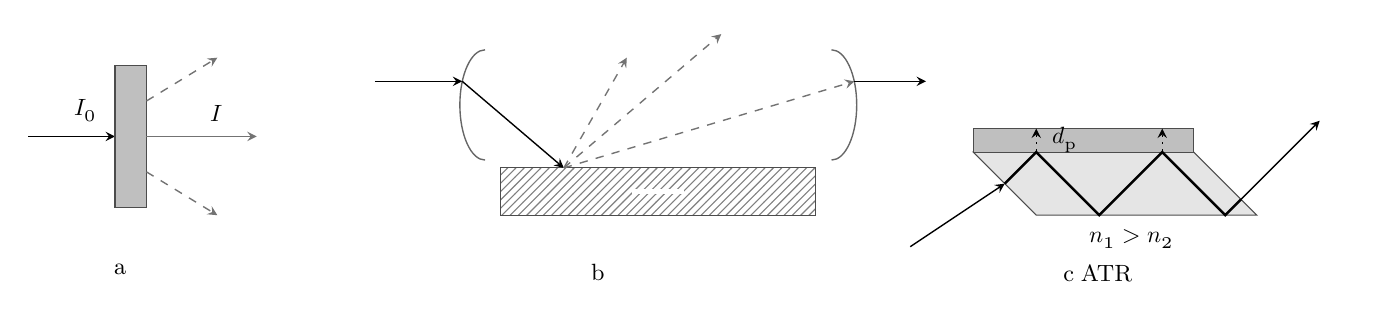
\begin{tikzpicture}[x=1mm,y=1mm,>=stealth,
  beam/.style={thinline,->},
  weakbeam/.style={thinline,->,draw=black!55},
  scat/.style={thinline,->,draw=black!55,dashed},
  samp/.style={draw=black!70,fill=black!25},
  xtal/.style={draw=black!70,fill=black!10}]
% ---------------- (a) 透射 ----------------
\draw[beam] (2,20) -- (13,20);
\node[anchor=south] at (7.5,20.6) {入射光 $I_{0}$};
\filldraw[samp] (13,11) rectangle (17,29);
\node[anchor=north] at (15,10.4) {样品片};
\draw[weakbeam] (17,20) -- (31,20);
\node[anchor=south] at (24,20.6) {透射光 $I$};
\draw[scat] (17,24.5) -- (26,30);
\draw[scat] (17,15.5) -- (26,10);
\node[anchor=west] at (26.5,30) {散射损失};
\node[anchor=north] at (17,5) {（a）透射：光穿过体相};
% ---------------- (b) 漫反射 ----------------
\filldraw[samp,pattern=north east lines,pattern color=black!50] (62,10) rectangle (102,16);
\node[fill=white,inner sep=1pt] at (82,13) {多次散射与吸收};
\node[anchor=north] at (81,8.6) {松散粉末（不压片）};
\draw[draw=black!60,thinline] (60,31) arc[start angle=90,end angle=270,x radius=3.2mm,y radius=7mm];
\draw[draw=black!60,thinline] (104,31) arc[start angle=90,end angle=-90,x radius=3.2mm,y radius=7mm];
\node[anchor=south] at (60,31.4) {收集镜};
\node[anchor=south] at (104,31.4) {收集镜};
\draw[beam] (46,27) -- (57.1,27);
\draw[beam] (57.1,27) -- (70,16);
\node[anchor=south east] at (46,27.6) {入射光};
\draw[scat] (70,16) -- (78,30);
\draw[scat] (70,16) -- (90,33);
\draw[scat] (70,16) -- (106.9,27);
\draw[beam] (106.9,27) -- (116,27);
\node[anchor=south] at (114,27.6) {到检测器};
\node[anchor=north] at (81,5) {（b）漫反射：光在粉末中散射后返回表面};
% ---------------- (c) ATR ----------------
\filldraw[xtal] (122,18) -- (150,18) -- (158,10) -- (130,10) -- cycle;
\filldraw[samp] (122,21) -- (150,21) -- (150,18) -- (122,18) -- cycle;
\node[anchor=west] at (151.5,21) {样品};
\draw[dotted,thinline,->] (130,18.2) -- (130,21);
\draw[dotted,thinline,->] (146,18.2) -- (146,21);
\node[anchor=west] at (130.8,19.6) {$d_{\mathrm{p}}$};
\draw[beam] (114,6) -- (126,14);
\draw[mainline] (126,14) -- (130,18) -- (138,10) -- (146,18) -- (154,10) -- (156,12);
\draw[beam] (156,12) -- (166,22);
\node[anchor=east] at (113.6,6.6) {入射光};
\node[anchor=west] at (166.4,22) {出射光};
\node[anchor=north] at (140,9.4) {全反射晶体（$n_{1}>n_{2}$）};
\node[anchor=north] at (142,5) {（c）ATR：光在晶体中多次全反射};
\end{tikzpicture}
\caption{三种常用模式中光与样品的相互作用方式对比。读者应看三处：\textbf{光在样品中走的
路径}（穿过体相／在颗粒间多次散射后返回／在晶体内部多次全反射）、\textbf{作用体积}
（体相、表层粉末、表面亚微米层）、以及由此决定的\textbf{样品形态与含水量要求}——透射要求
样品能做成自支撑薄片且散射弱，含水或易碎的粉末难以制样；漫反射直接用松散粉末，不破坏样品
形态，但粉末堆积状态会直接改变基线；ATR 只探测紧贴晶体的表面层，样品形态几乎不受限，但
要求接触紧密、晶体折射率大于样品。图中光路为示意，未按真实比例绘制。\schemamark
\figsrc{据 S1（上册）图 7-10、图 7-14、图 7-16，书内 p.428、p.432、p.433 / PDF p.447、
p.451、p.452 改绘。}}
\label{fig:paths}
\end{figure}

\begin{keycond}
选型的三句口诀（由式~\eqref{eq:art} 直接推出）：\textbf{吸收适中、散射弱 $\rightarrow$ 透射}；
\textbf{散射或反射能量大 $\rightarrow$ 漫反射}；\textbf{吸收很强、近乎不透明 $\rightarrow$
发射}。再叠加两条信息深度要求：只要表面层信息、样品又无法制样时选 ATR；要的是表面单层、
且不允许体相与气相干扰时选 SFG。没有一种池或附件能满足所有研究要求，这也是原位池至今仍多
为自行设计加工的原因 \src{S1 §7.1.1，书内 p.421 / PDF p.440}。
\end{keycond}

\subsubsection{透射红外吸收光谱：默认选项与它的代价}

透射法技术相对简单、适用面广；代价集中在\textbf{制样与散射}，其余条件集中列在下框中。

\textbf{（1）制样与散射}。负载催化剂折射率高，散射是获得好谱图的主要障碍：散射损失取决于样品与
周围介质的折射率差、入射光波长与颗粒大小，因此\textbf{颗粒应小于所用红外波长}以降低散射；
近红外区散射损失很大，远红外区虽散射小但体相吸收大，故一般在 \qty{1000}{cm^{-1}} 以下不
推荐透射测量 \src{S1 §7.1.1，书内 p.418 / PDF p.437}。常用的 KBr 压片与石蜡糊法因稀释剂
吸收与压力效应，\textbf{不能用于原位研究}。原位研究用\textbf{自支撑片}：不加稀释剂直接把
粉末压成薄片，具体条件集中列在下框
\src{S1 §7.1.1，书内 p.418—419 / PDF p.437—438}。

\begin{measure}
\textbf{透射原位的常规测量条件}（据 S1 §7.1.1，书内 p.418—422 / PDF p.437—441）：
（1）\textbf{片}：直径 $15$--$25$~mm 以充满光束，压力 $70$--$110$~atm（约 $7$--$11$~MPa），
加料均匀、必要时垫云母片；
（2）\textbf{厚度判据}：\qty{4000}{cm^{-1}} 处透射率落在 $10\%$--$30\%$——太厚则吸附带饱和
且可利用能量下降，太薄则吸附物种信号太弱；
（3）\textbf{池}：能在池内完成焙烧、流动氧化还原、抽高真空（脱气）、吸附与反应；可随时
移出或移入光路而不受上述处理影响；记录谱图时不受气相组分影响；池本底干扰尽量小；
（4）\textbf{窗口}：\ce{NaCl}、\ce{KBr} 范围宽但潮解；\ce{CaF2}、\ce{BaF2} 耐水却忌铁盐
溶液、对热与振动敏感；\ce{ZnSe} 近年较常用；高温池窗口与法兰需水冷保护；
（5）\textbf{背景}：在同温度、同气氛下采集，并用热电偶直接测样品（或样品架）温度。
\end{measure}

\begin{pitfall}
\textbf{池内样品温度不等于设定温度。}带水冷与外加热的简单池，外壁与中心样品之间存在温差；
高温石英池在温度高时池壁与样品的实际温差最大可达 $100\,^{\circ}\mathrm{C}$
\src{S1 §7.1.1，书内 p.419 / PDF p.438}。因此\textbf{必须用热电偶直接测样品（或样品架）
温度并在文中说明测温方式}；用炉温代替样品温度，会把温度效应误读成物种变化。
\tocheck{未对照原页面图像：简单池「$200\,^{\circ}\mathrm{C}$ 时温差小于 $2\,^{\circ}\mathrm{C}$」
一项，OCR 作「小于 27 ℃」（书内 p.419 / PDF p.438），数值疑为 2 ℃，待核。}
\end{pitfall}

\subsubsection{漫反射红外光谱（DRIFT）：松散粉末与 Kubelka--Munk}

漫反射把「散射」从损失变成信号来源：光斜入射到松散粉末，在颗粒间多次散射后一部分返回表面，
由离轴椭圆镜收集（图~\ref{fig:paths}b）。它可以直接测量松散粉末，避免压片造成的扩散影响，
很适用于散射很强的样品；通常用 DRIFT 或 DRIFTS 表示漫反射傅里叶变换红外光谱。其吸收光谱
用 Kubelka--Munk 函数描述 \src{S1 §7.1.2，书内 p.427 / PDF p.446}：

\begin{equation}\label{eq:km}
\frac{K}{S}=\frac{\left(1-R_{\infty}\right)^{2}}{2R_{\infty}}
\end{equation}

式中 $K$ 为吸收系数（频率的函数），$S$ 为散射系数，$R_{\infty}$ 为无限厚样品的反射比（一般
厚度在几毫米即可满足该条件）。

\begin{keycond}
式~\eqref{eq:km} 把反射比换算成与浓度近似成正比的量，但成立前提是\textbf{散射系数 $S$ 在
测量过程中恒定}——也就是粒度、装填密度、压实程度都不变。这决定了 DRIFT 的使用纪律：
同一系列实验必须保持\textbf{同一批样品、同一粒度、同一装填方式}，背景必须在\textbf{同一
温度与同一气氛}下采集；否则基线漂移会被误当作吸附物种的增减。
\tocheck{未对照原页面图像：式~\eqref{eq:km} 的符号约定（$R_{\infty}$ 为反射比还是反射率、
是否取负对数）与 $K$、$S$ 的定义，OCR 残缺（书内 p.427 / PDF p.446）。}
\end{keycond}

为了做原位研究，已发展出可控气氛与压力的原位漫反射池，可在室温至 $400$--$500\,^{\circ}\mathrm{C}$、
真空或加压条件下工作，并可配气路与产物分析
\src{S1 §7.1.2，书内 p.428 / PDF p.447}。相对透射，DRIFT 的代价是定量更弱、谱带形状受
Kubelka--Munk 变换影响，气相干扰也更难扣除（光路在池内是开放的散射几何）。

\subsubsection{衰减全反射红外光谱（ATR）：只取表面层}

ATR 以光在两种介质界面发生全内反射为基础。当光从光密介质（折射率为 $n_{1}$ 的反射元件）
射向光疏介质（折射率为 $n_{2}$ 的样品），且入射角 $\theta$ 大于临界角 $\theta_{\mathrm{c}}$
时发生全反射：

\begin{equation}\label{eq:crit}
\sin\theta_{\mathrm{c}}=\frac{n_{2}}{n_{1}}\qquad\left(n_{1}>n_{2}\right)
\end{equation}

全反射并非光完全不进入样品：光会在样品表面下一定深度才返回，若该层在特定频率有吸收，反射
光中对应频率就出现吸收带，这就是 ATR 光谱。穿透深度 $d_{\mathrm{p}}$ 定义为辐射波电场强度
衰减至表面处 $1/e$ 的距离：

\begin{equation}\label{eq:dpen}
d_{\mathrm{p}}=\frac{\lambda_{0}}{2\pi\sqrt{n_{1}^{2}\sin^{2}\theta-n_{2}^{2}}}
\end{equation}

式中 $\lambda_{0}$ 为\textbf{真空波长}（约 $2.5$--$25$\,µm），$\theta$ 为入射角。
\tocheck{原书式（书内 p.432 / PDF p.451）写作 $d_{\mathrm{p}}=\lambda_{1}/[2\pi n_{1}
\sqrt{\sin^{2}\theta-(n_{2}/n_{1})^{2}}]$，同时把 $\lambda_{1}$ 定义为「介质内波长」——
若分子已用 $\lambda_{1}=\lambda_{0}/n_{1}$，分母不应再出现 $n_{1}$，原书此处符号定义冲突。
本书按倏逝场振幅 $1/e$ 定义改写为上式的真空波长形式。}
\textbf{数值自检}：$\lambda_{0}=\qty{10}{\micro m}$、$n_{1}=2.4$、$n_{2}=1.5$、
$\theta=45^\circ$ 时 $\sqrt{n_{1}^{2}\sin^{2}\theta-n_{2}^{2}}=\sqrt{0.63}=0.7937$，
得 $d_{\mathrm{p}}=\qty{2.005}{\micro m}$。若照原书写法把 $\lambda_{1}=\lambda_{0}/n_{1}$
再除一次 $n_{1}$，会得到 $\qty{0.8355}{\micro m}$——\textbf{系统性低估穿透深度，误差恰为一个
因子 $n_{1}$}。
由式~\eqref{eq:dpen} 可知：\textbf{穿透深度与真空波长成正比}，波长越长探测越深；入射角
接近临界角时穿透深度急速增大，远大于临界角时变化平缓
\src{S1 §7.1.4，书内 p.432 / PDF p.451}。这带来一个常被忽略的后果：
\textbf{同一张 ATR 谱中不同波数的探测深度不同}，谱带的相对强度因此失真，跨波数比较峰高
必须先作深度校正。

为增强吸收峰强度，现代 ATR 附件多用多重全反射：光在梯形（或平行四边形）晶体中多次全反射，
次数可达 $20$--$50$ 次，总穿透深度大大增加。反射次数由晶体几何决定
\src{S1 §7.1.4，书内 p.433 / PDF p.452}：

\begin{equation}\label{eq:nref}
N=\frac{l}{d}\cot\theta
\end{equation}

式中 $l$ 为全反射晶体的长度，$d$ 为两个反射面间的距离，$\theta$ 为入射角。$l$ 与 $d$ 固定，
减小入射角可增加反射次数，是提高 ATR 信号强度的有效办法。

\tocheck{未对照原页面图像：式~\eqref{eq:dpen} 已按倏逝场振幅 $1/e$ 定义改写为真空波长形式
（见该式下方的说明与数值自检）；式~\eqref{eq:nref} 的 $l$、$d$ 定义与是否需要厚度修正
仍待核对（书内 p.432—433 / PDF p.451—452）。}

晶体材料的选择取决于折射率、化学稳定性、光谱范围与机械强度。由于大多数有机物折射率在
$1.5$ 以下，按 $n_{1}>n_{2}$ 的要求，ATR 晶体折射率须大于 $1.5$，常用 KRS-5、\ce{ZnSe}、
\ce{Ge}、\ce{Si} 等；晶体做成菱形，样品放在两个较大的侧面上，几何尺寸受全反射次数与光源
光斑大小约束 \src{S1 §7.1.4，书内 p.433 / PDF p.452}。其中 \ce{ZnSe} 光谱范围宽、化学
稳定性好，\ce{Ge} 极硬但透光范围窄，KRS-5 质软、有毒且受强酸与烷烃类物质影响。

\begin{pitfall}
\textbf{ATR 的成败几乎全在「接触」。}倏逝波只与紧贴晶体的那一层样品耦合，接触不良时信号
骤降、谱带畸变，且不同波数处接触状态不同会造成假峰。粉末样品的原位气固 ATR 因此受限：
必须加压夹紧，而加压本身又会改变床层孔隙与传质——这一条与下文「压片压力」的误判是同一
类问题。ATR 给出的是表面层信息，\textbf{不能代表体相组成}。
\end{pitfall}

\subsubsection{其余四种模式各自解决什么问题}

\textbf{红外发射光谱}不用外光源，直接测样品自身的热辐射，适用于吸收很强、既透不过也反射
不回来的样品，并天然适合高温条件。依据是 Kirchhoff 定律：热平衡下发射率等于吸收率
（$a=e$），配合 $t+r+a=1$（反射率极小时化为 $e=1-t$），发射光谱可换算为透射光谱。原位
发射池可在池内完成真空处理、氧化还原与反应，样品温度可到 $700\,^{\circ}\mathrm{C}$，衬底
常用镀金不锈钢片以避免高温氧化与反应。因绝对发射率难以测定，实践中以同温度下样品支撑片
（近似灰体）的本底谱 $L_{\mathrm{r}}(T)$ 作参考，报出\textbf{相对发射度}
$RE=L_{\mathrm{s}}(T)/L_{\mathrm{r}}(T)$，可同时扣除支撑片发射与仪器光路的吸收和发射
\src{S1 §7.1.3，书内 p.429—431 / PDF p.448—450}。
\tocheck{未对照原页面图像：相对发射度的定义式 $RE=L_{\mathrm{s}}(T)/L_{\mathrm{r}}(T)$ 与
$e=L_{\mathrm{s}}/L_{\mathrm{bb}}$ 的符号，以及「发射度（emittance）」与「发射率
（emissivity）」两个术语的中文用法（书内 p.431 / PDF p.450）。}

\textbf{红外合频（SFG）}是表面与界面专属的技术。非线性光学过程要求介质非中心对称，一般
物质体相是中心对称的，只有表面与界面处对称性被破坏才产生二次非线性现象；可调红外光与
固定可见光同时照射表面，取和频信号即得表面振动光谱。它的选律是\textbf{振动模式必须同时
具有红外与拉曼活性}，信号不载体相与气相贡献，可在 $250$--$1000$~K、超高真空至几个大气压
范围内工作，从而把超高真空模型研究与真实反应条件连接起来。局限同样明确：\textbf{只能用于
平整表面}，粗糙与多孔表面不能研究；高功率激光可能损伤样品；红外频率范围有限（约
$1100$--$\qty{4000}{cm^{-1}}$）\src{S1 §7.1.5，书内 p.434—436 / PDF p.453—455}。

\textbf{时间分辨红外（TR-IR）}按时间尺度选技术：分钟至小时级用普通稳态采谱；秒至毫秒级用
快速扫描 FTIR（动镜加速，最快几十毫秒完成一次扫描），信噪比的损失可用「同一动力学过程
重复多次、按时间序列累加平均」补回；纳秒至微秒级用步进扫描（动镜停在固定位置采集扰动响应，
再逐点移动）配快速 MCT 检测器，要求过程高度可重复；飞秒至皮秒级用泵浦--探测方案，以光学
延迟平台控制探测光与激发光的时间差。步进扫描保持了 FTIR 的高分辨率与波数准确度，但灵敏度
低于光栅扫描，且难以直接抽取某一波数的动力学曲线
\src{S1 §7.1.6，书内 p.436—440 / PDF p.455—459}。

\textbf{近场光学红外（Nano-FTIR）}突破衍射极限。传统红外成像的分辨率受衍射限制，中红外
波段只有微米量级；把扫描近场光学显微镜与 FTIR 结合，探测金属化探针针尖尖端形成的、尺度与
针尖曲率半径相当的纳米增强场与样品的相互作用，可实现纳米级分辨的光谱采集，目前最高空间
分辨率约 \qty{20}{nm}。探针以频率 $\Omega$ 振动使近场信号被周期调制，对基频或高次谐波解调
即可得到纯近场信号 \src{S1 §7.1.7，书内 p.440—441 / PDF p.459—460}。它的限制是扫描慢、
只测针尖附近的极小区域、定量很弱。

\subsection{原位与 operando：差别必须写清}

这是本章标题的落点，也是最容易被混用的一对词。

\begin{principle}
\textbf{原位（in situ）}：\textbf{只在反应条件下测谱}。样品处于反应温度、压力与气氛中，
光谱给出表面物种「有什么、何时出现、何时消失」。但多数原位池不同时测量反应速率与产物分布，
因此\textbf{无法把表面物种与催化性能直接关联}——当原位谱在真空或非反应条件下测量时，这一
缺陷尤其突出 \src{S1 §7.1.8，书内 p.441 / PDF p.460}。

\textbf{operando}：\textbf{在工作状态下同时进行光谱表征与催化性能测量}，即红外（或其他
谱学）与在线产物分析（质谱、色谱）同时进行，从而得到「反应结构」与「反应中间物」的直接
关系，建立动态构效关系。催化剂表面随环境条件（温度、压力、气相或液相组成）动态变化，
\textbf{只有在反应条件下、并同时知道反应速率，才能谈构效关系}——这就是 operando 存在的
理由 \src{S1 §7.1.8，书内 p.441 / PDF p.460}。
\end{principle}

一句话概括：\textbf{operando $=$ in situ $+$ 同时测催化性能}。原位说「表面上有什么」，
operando 才说「这些物种与反应速率有什么关系」。

\textbf{稳态同位素瞬态动力学分析（SSITKA）}是重要的 operando 红外技术。它在等温等压下快速
用同位素瞬态物种替换其中一种反应物（例如以 \ce{^{13}CO} 替换 \ce{^{12}CO}），同时切换惰性
气体以确定反应器中滞留气体的组成；由于等温等压，催化剂表面在切换过程中没有变化。反应物与
产物用在线色谱定量，瞬态响应物种用质谱记录，通过分析原物种与同位素物种随时间的变化规律，
可得到分子水平的机理信息与中间体的动力学量（浓度、反应活性、速率常数），从而把真正的中间物
与旁观物种区分开 \src{S1 §7.1.8，书内 p.442 / PDF p.461}。

\begin{keycond}
operando 池必须同时满足三组互相牵制的要求，因此设计必然是折中：（1）\textbf{光谱可测}——
窗口透光范围、光程与样品量足以给出可分辨的谱带；（2）\textbf{反应器行为接近真实}——传质
传热、空速、压力、产物滞留体积尽量接近实用反应器；（3）\textbf{产物可定量}——死体积小、
响应快，才能把毫秒级的表面变化与产物信号对齐。报告 operando 结果时应给出池型、空速、样品
量与产物分析的响应时间；缺失这些，表面物种与速率的「同步」就无从判断。
需同时注意两条常见的鸿沟：压力鸿沟（超高真空模型研究 vs 常压／高压真实反应）与材料鸿沟
（单晶与模型薄膜 vs 实际负载催化剂），SFG 一类技术正是为跨越前者而发展起来的。
\end{keycond}

\subsection{从原始谱图到结论}

\begin{dataflow}
（1）\textbf{同条件背景}：在同一温度、同一气氛（最好同一池、同一光程）下采集背景；高温时
还需扣除样品热发射的贡献，否则水、\ce{CO2} 与热辐射都会被读成吸附带。
（2）\textbf{差谱与基线}：以吸附前（或惰性气氛下）的谱作参考做差谱，检查差谱中是否出现
负峰或位置漂移的伪峰——出现即说明背景与样品状态不一致，应重测而不是解释。
（3）\textbf{峰位归属}：以基团特征频率与已知参考谱比对；吸附引起的频率位移（相对气相或
物理吸附态）本身就携带键合方式的信息。
（4）\textbf{变量实验}：改变温度、覆盖度、分压或同位素，看各谱带是同步变化还是有先有后；
\textbf{只有先后次序才能给出动力学信息}。
（5）\textbf{与产物分析关联}：把谱带强度的时间曲线与产物生成速率放在同一时间轴上比较
（operando），同步变化的物种才是候选中间物。
（6）\textbf{定量}：只有在同一系列、同一制样与同一条件下比较峰面积；要给出覆盖度必须说明
标定方式（式~\eqref{eq:beer} 的边界见前文关键条件）。
\end{dataflow}

\begin{obs}
（教学设定）某原位透射实验中，切换反应气后 $2100$--$\qty{2050}{cm^{-1}}$ 区间的谱带在
$30$~s 内明显增强；而池出口质谱给出的产物信号约在 $90$~s 后才达到新的稳态。
\end{obs}

\begin{infer}
谱带增强\textbf{先于}产物响应，说明该物种的生成不依赖产物积累，与「产物二次吸附」这一类
解释不符；但这\textbf{不足以}证明它是催化循环内的中间物——它也可能是与反应无关的旁观物种，
或仅仅是池内气相分子在冷点上的物理吸附。要区分，需要同位素切换（看产物中是否出现同位素
标记）或瞬态实验（看它的消耗速率是否与产物生成速率同量级）。
\end{infer}

\subsection{误判与边界}

\begin{pitfall}
\textbf{（1）原位池的传质与传热滞后。}池内滞留体积大、气体置换需要时间，气相组成的变化
与样品实际感受到的变化之间存在时间差；同时池内存在温度梯度（前文所述的池壁与样品温差）。
后果是：表面物种的响应时间被高估，先后次序可能被颠倒。对策是用质谱或色谱同步监测出口
组成以估计滞后时间，并在同一篇工作中固定气速与样品量。

\textbf{（2）自支撑片的厚度与压片压力改变样品本身。}压力过低片子易碎、厚度不均；压力过高
会把颗粒压实，改变孔隙结构与表面可及性——对分子筛与高比表面氧化物尤其明显，此时测到的
已不是真实催化剂表面的行为。同一系列实验必须固定压力与厚度，并记录片重与厚度。

\textbf{（3）水与 \ce{CO2} 的干扰。}它们是大气与管路中最常见的杂质，气相谱带与表面羟基、
碳酸盐、甲酸盐物种的谱带重叠，极易误判。\supp{补充：\ce{CO2} 的反对称伸缩振动在约
\qty{2349}{cm^{-1}}，水的弯曲振动在约 \qty{1600}{cm^{-1}}、伸缩振动在
$3400$--$\qty{3600}{cm^{-1}}$ 附近，都是原位谱图中最常出现的干扰位置。}对策是充分吹扫或
抽真空、并在同条件下取背景；但要注意\textbf{不能一律扣除}——反应中真实生成的表面碳酸盐、
甲酸盐物种恰恰就在这些位置，把它们当干扰扣掉会删掉真正的结论。

\textbf{（4）「看到谱带变化」不等于「看到催化循环内的中间物」。}谱带出现或消失只说明表面
浓度变了，并没有检验该物种是否与催化循环的速率相关。判据至少要有其一：它与产物生成的
速率同量级并可建立定量关系；同位素切换或瞬态实验给出预期响应；预吸附该物种会改变（或不
改变）转化频率。缺少这些证据，只能称为「反应条件下的表面物种」，不能称为中间物。

\textbf{（5）升温带来的峰位移与热发射。}温度升高时键长与吸附强度变化会使峰位移动，高温下
样品的热发射还会叠加入透射谱形成假峰。跨温度比较峰位时，应先用同一温度下的背景扣除，并
避免把几十 \unit{cm^{-1}} 的整体位移解释为「生成了新物种」。
\end{pitfall}

\begin{crosscheck}
红外只给振动信息，必须与其他方法互证才能支撑结论。（1）\textbf{与拉曼互补}：红外活性源于
偶极矩变化，拉曼活性源于极化率变化，中心对称分子遵循互斥规则；载体在
\qty{1000}{cm^{-1}} 以下不透光的问题可用拉曼绕开，两者对同一物种的归属一致时才可确信。
（2）\textbf{与程序升温脱附、化学吸附、质谱联用}：给出吸附量与脱附温度，与红外的物种归属
相互印证；活性位数目的定量属于化学吸附方法的范围（\chapref{ch:05}）。
（3）\textbf{与 X 射线衍射等体相方法联用}：区分表面物种与体相变化（\chapref{ch:04}）。
（4）\textbf{与在线色谱／质谱联用}构成 operando，把表面物种与反应速率关联；催化剂比表面
与孔结构的变化则回到物理吸附（\chapref{ch:01}）。
若红外与拉曼、或红外与脱附实验给出矛盾结论，应先检查标定、基线与样品状态，而不是择一采信。
\end{crosscheck}

\srcnote{本分片来源：S1（上册）§7.1（含 §7.1.1—§7.1.8），书内 p.413—447 / PDF p.432—466。
其中式~\eqref{eq:art}、式~\eqref{eq:km}、式~\eqref{eq:crit}--\eqref{eq:nref} 的变量定义按
正文 OCR 重建，系数与符号约定存疑处已在文中以「待核对」标出；图~\ref{fig:paths} 为据原书
图 7-10、7-14、7-16 改绘的示意光路，非原图描摹。§7.2 及以后的探针分子与反应机理内容
见分片 b/c。}
}{}
\IfFileExists{chapters/parts/ch07-b.tex}{% ================================================================
% chapters/parts/ch07-b.tex —— 第 7 章 原位红外光谱方法（分片 b）
% 覆盖：原书 §7.3（探针分子、金属催化剂表征）与 §7.4.2—7.4.4
%        （表面羟基、固体表面酸性、氧化物表面氧物种）
%        书内 p.448—488 / PDF p.467—507
% 注：原书 §7.2「吸附分子的特征和它的红外光谱诊释」属分片 a 的范围，
%     本节只从「判断」角度引用其结论，不重复叙述。
% 版式自查（WRITER_BRIEF §7.3）：单栏版心 165 mm；\onecolwidth = 0.80\textwidth ≈ 132 mm。
%   图 \ref{fig:ch07b-co-model} 用 groupplot，3 列：
%     3×48 + 2×8 = 160 mm，加左侧轴标签 ≈3 mm → ≈163 mm ≤ 165 mm  ✓
% ================================================================

\subsection{探针分子的选择与红外光谱诊释}

\begin{probout}
拿到一张吸附分子的红外谱，问题从来不是「有没有峰」，而是三个判断：峰在哪
（位置）、峰多高（强度）、峰随条件怎么动（位移方向与幅度）。三者分别对应
表面有什么位、位有多少、位上的电子状态如何。本节要输出的不是某个体系的
具体归属，而是一套可复用的判读路径：先选对探针分子，再用位置定类型、用
强度定数量、用位移定电子状态，最后回查各环节的干扰。
\end{probout}

\subsubsection{从谱带到表面位的判读链条}

\begin{principle}
吸附分子的红外光谱与它吸附前的光谱相比，除了可能出现新的「表面键」伸缩
振动谱带，原有振动频率也会位移；若吸附后分子化学结构改变（如双键打开），
振动改变更大\src{S1 §7.2，书内 p.444 / PDF p.463}。判读因此有两条依据：
\begin{itemize}
  \item \textbf{位置}定「位」的类型。同一探针分子在不同性质的表面位上以不同
        方式键合，其基团特征频率落在不同区间，故位置先给类型。
  \item \textbf{强度}定「位」的数量。定量只能建立在朗伯—比尔定律之上：
\end{itemize}
\begin{equation}
  A=\varepsilon\,c\,l
  \label{eq:ch07b-beer}
\end{equation}
式中 $A$ 为积分吸光度（谱带面积），$\varepsilon$ 为该谱带的积分消光系数，
$c$ 为吸光物种的表面浓度（单位面积上的摩尔数或分子数），$l$ 为有效光程。
若把探针分子近似为「一位一分子」的化学计量滴定，则 $c$ 即该类型表面位的
表面密度。

\textbf{成立条件（三条必须同时成立）}：一是化学计量数已知且不随组成变化；
二是各吸附构型（线式／桥式／多点配位）的消光系数已知且恒定；三是不同样品
的有效光程 $l$ 可比。三条中任意一条不成立，强度就只是相对强弱，不能再读
成位密度。
\end{principle}

\begin{measure}
探针分子的谱带位置本身对条件很敏感，测量时必须同时锁定：
(1) \textbf{温度}——吸附温度与抽空温度共同决定留下哪些物种，例如吡啶需在
$150\,\degC$ 抽空以排除物理吸附（见 \S\,\ref{sec:ch07b-oxide}）；
(2) \textbf{覆盖度}——同一吸附位的 $v(\mathrm{C{-}O})$ 会随覆盖度漂移，故对比样品
须在同一平衡压力与同一抽空时间下测；
(3) \textbf{样品形态}——自支撑片的厚度与散射本底直接进入方程
\equref{eq:ch07b-beer} 的 $l$，厚度不同的片强度不可直接比；
(4) \textbf{本底}——须对同一样品在同一条件下采集吸附前本底谱并作差谱。
\end{measure}

\subsubsection{常用探针分子及其适用范围}

选择探针分子的实质是选择它的\textbf{碱性（或酸性）强度}与\textbf{分子尺寸}
两个参数。碱性太强的探针会把弱酸位一并质子化，从而抹平强度差异；尺寸太大
的探针进不了小孔，只能报告外表面。表 \ref{tab:ch07b-probes} 给出本节与
\S\,\ref{sec:ch07b-oxide} 反复用到的五种探针。

\begin{table}[htbp]
\centering
\caption{常用探针分子的适用范围、谱带位置与干扰}
\label{tab:ch07b-probes}
\small
\begin{tabularx}{\onecolwidth}{@{}>{\raggedright\arraybackslash}p{13mm}
 >{\raggedright\arraybackslash}p{30mm}
 >{\raggedright\arraybackslash}p{29mm}
 >{\raggedright\arraybackslash}X
 >{\raggedright\arraybackslash}X@{}}
\toprule
探针 & 测什么 & 谱带位置区间$^{\mathrm{a}}$ & 定量前提 & 主要干扰 \\
\midrule
CO &
 金属位（顶位／桥位）、氧化物表面 L 酸位与配位不饱和阳离子；
 \textbf{不与 B 酸位作用} &
 顶位／L 酸位配位 $>2000$；桥位 $<2000$；
 氧化物上 L 酸位约 $2150$—$2200$ &
 需各类吸附构型的积分消光系数；
 需按覆盖度归一 &
 气相 CO 的振动—转动谱带（$P$／$R$ 支）；
 桥位与顶位谱带重叠；
 CO 在金属上可歧化生成 $\ce{CO2}$ 与表面碳 \\
吡啶 &
 L 酸位与 B 酸位的同时区分（环变形振动对成键方式敏感） &
 B 酸位 $1540$、L 酸位 $1450$（均为环变形振动）；
 另有 $1490$ 带为两类位共有 &
 需 $150\,\degC$ 抽空扣除物理吸附与气相；
 需分别标定两类位的消光系数 &
 物理吸附吡啶（室温可抽除）残留；
 探针在强酸位上的质子化产物本身即被测物种 \\
$\ce{NH3}$ &
 L 酸位与 B 酸位（主要以变形振动区分） &
 L 酸位配位 $\ce{NH3}$：$3330$、$1610$；
 B 酸位 $\ce{NH4+}$：$3230$、$1432$ &
 碱度大，滴定可近化学计量；
 但强弱酸位同时被滴定 &
 \textbf{碱性过强}，会把弱酸位一并滴定而掩盖其差异；
 易与表面羟基形成氢键物种，产生额外谱带 \\
$\ce{CO2}$ &
 表面碱性位（碱性氧位）、表面碳酸盐与甲酸盐物种 &
 碳酸盐／羧酸盐的 $v_{\mathrm{as}}(\mathrm{OCO})$ 约 $1572$、
 $v_{\mathrm{s}}(\mathrm{OCO})$ 约 $1369$；
 甲酸盐 $\nu(\mathrm{C{-}H})$ 约 $2870$、$\delta(\mathrm{C{-}H})$ 约 $1379$ &
 需先扣除表面预存碳酸盐保护层；
 需已知各碳酸盐构型的消光系数 &
 碱性氧化物表面天然覆盖一层稳定碳酸盐；
 多种碳酸盐构型谱带重叠 \\
$\ce{CH3CN}$ &
 表面羟基的酸性强度（由氢键引起的羟基位移反推） &
 以羟基伸缩带位移读数：二氧化硅—氧化铝上
 $3750$ 一带吸附后分裂为两个峰 &
 需记录吸附前后羟基带的半宽与位移；
 需同时测 OD 形式作对照 &
 探针在强酸位上可被质子化，生成物种的谱带与氢键物种不同；
 液态／物理吸附态的谱带覆盖 \\
\bottomrule
\end{tabularx}

\vspace{1pt}
{\srcsize $^{\mathrm{a}}$ 单位 $\mathrm{cm^{-1}}$。CO 在氧化物 L 酸位上的
$2150$—$2200$ 区间与在金属顶位上的 $>2000$ 区间在数值上有重叠，
两者必须靠样品体系（有无金属组元）与共吸附实验区分，不能只凭波数。
CO 位置的区间系按本书所给实例归纳，具体体系的数值须逐例核对。}
\end{table}

\begin{dataflow}
从一张吸附谱到一个结论，应当走完四步：
\textbf{(1) 定本底与差谱}：取得同一样品吸附前谱，作差得吸附物种谱。
\textbf{(2) 分峰定位置}：对重叠区作分峰，读出各组分的位置与面积；只有位置
确定后，才谈得上归属。
\textbf{(3) 用位置定类型}：按 \tabref{tab:ch07b-probes} 的区间先给「哪一类位」，
再在同类位内部用共吸附或同位素实验细分。
\textbf{(4) 用面积与位移定量}：面积经方程 \equref{eq:ch07b-beer} 换算成表面
浓度，位移用于判读电子转移方向与程度。
四步中任何一步的中间结论都不得越过下一步直接当结论用——尤其是「位置」
只能给类型，不能给强度。
\end{dataflow}

\begin{pitfall}
\textbf{误判一：把谱带位移作单因素归因。}同一吸附位的 $v(\mathrm{C{-}O})$
位移至少有四个来源：吸附构型改变（顶位／桥位／多点配位）、覆盖度变化、
金属组元的电子效应、以及偶极—偶极耦合造成的集体位移。本书的数据正好
把前两者的量级暴露出来：$\mathrm{Pd{-}Ag}$ 体系中覆盖度从高到低变化引起的
CO 化学位移只有约 $9\;\mathrm{cm^{-1}}$，而合金组成变化引起的位移达
$29\;\mathrm{cm^{-1}}$\src{S1 §7.3.2，书内 p.453 / PDF p.472}。因此
「位移大就是电子效应」在量级上可以成立，但\textbf{必须先给出几何效应
与覆盖度效应的上限估计}，否则无法排除它们。

\textbf{误判二：忽略消光系数差异而直接比强度。}顶位与桥式 CO 的积分消光
系数不同，$\ce{NH3}$ 在 L 酸位与 B 酸位上的变形振动消光系数也不同。
若拿两类谱带的面积直接相比，得到的比值中混入了消光系数的比值。

\textbf{误判三：忽略探针分子自身的反应。}CO 在金属表面上可发生歧化，
生成的 $\ce{CO2}$ 与表面碳会同时改变谱图与表面状态；吡啶在强酸位上会
质子化，其质子化产物恰恰是被测物种，二者在谱上不易分开。

\textbf{误判四：自支撑片厚度不一而直接比较强度。}不同样品压片厚度不同，
方程 \equref{eq:ch07b-beer} 中的 $l$ 就不同。凡跨样品比较强度，必须先归一：
常用做法是以分子筛骨架振动或二氧化硅的 $1860\;\mathrm{cm^{-1}}$ 附近
（二氧化硅骨架的倍频／组频）谱带为内标，或直接称量压片并记录厚度。
\end{pitfall}

\subsubsection{一个读图实例：从「峰在哪」到「位是什么」}

下面的实例取自本书对 $\ce{Pt{-}Ru/SiO2}$ 双金属催化剂的双探针研究
\src{S1 §7.3.1，书内 p.449—451 / PDF p.468—470}。请把它当作判读路径的
示范，而不是一个可以直接背下来的归属表。

\begin{obs}
在含 $38\%$ Ru 的 $\ce{Pt{-}Ru/SiO2}$ 上，CO 与 NO 混合气于室温竞争吸附，
抽空后测得：CO 吸附峰约在 $2065\;\mathrm{cm^{-1}}$，NO 吸附峰约在
$1550\;\mathrm{cm^{-1}}$，三个峰在室温抽空后都是稳定的。
随样品中 Ru 原子百分数增加（$10\%\to100\%$）：NO 峰相对 CO 峰的强度
增大；NO 吸收峰向高波数位移；CO 谱带强度减弱；CO 谱带向低波数位移，
对应位置由约 $2074\;\mathrm{cm^{-1}}$ 移到约 $2030\;\mathrm{cm^{-1}}$
\src{S1 表 7-（Pt-Ru 吸附数据），书内 p.450 / PDF p.469}。
\end{obs}

\begin{infer}
由「CO 峰在 $2065\;\mathrm{cm^{-1}}$ 以上、NO 峰在 $1550\;\mathrm{cm^{-1}}$
附近」这两个位置，结合两种探针在各金属上的成键差异，可推断 CO 主要吸附
在 Pt 中心上、NO 主要吸附在 Ru 中心上。这一步只用到了\textbf{位置}，
因此它只给出「哪种分子占哪类中心」，不给任何数量结论。

由「NO 峰强度随 Ru 含量增大而相对增强、CO 峰随之减弱」这一\textbf{强度}
变化，可进一步推断两种探针确实分别报告了两个组元的表面分数——这是把
强度当作表面组成的量度来用的前提。

由「CO 谱带随 Ru 含量增加而向低波数位移」这一\textbf{方向}，按
$d$—$\pi^{*}$ 反馈模型可推断：金属向 CO 的 $\pi^{*}$ 反键轨道反馈电子
的程度增加，$v(\mathrm{C{-}O})$ 因而降低。这一推断的强度弱于前两条：
位移方向支持电子转移的判断，但位移的\textbf{幅度}不能直接当作电子转移量，
理由见上文误判一。
\end{infer}

\begin{crosscheck}
三条互补的回查：
(1) 用已知分散度的单一金属样品（$\ce{Pt/Al2O3}$、$\ce{Ru/Al2O3}$）分别
标定两种探针在各自金属上的谱带位置与积分消光系数，再把同一套条件用到
双金属样品上；
(2) 用化学吸附（$\ce{H2}$、CO 吸附量）或 TPD 给出的表面总原子数与红外
定量结果对照，二者相符才说明「位置—强度」链条没有系统性偏差；
(3) 用同位素或共吸附实验独立验证电子转移方向，例如改变共吸附分子的
给电子能力，看位移方向是否随之翻转。
本书对 $\ce{Pt{-}Ru}$ 体系的结论正是靠化学吸附对照得到支持的
\src{S1 §7.3.1，书内 p.451 / PDF p.470}。
\end{crosscheck}

\subsection{红外光谱在金属催化剂表征中的应用}

\subsubsection{双探针法测定双金属催化剂的表面组成}

\begin{probout}
要输出的是\textbf{最表面层}的组成，而不是体相组成。合金催化剂的表面组成
常与体相明显不同，催化性能随之显著变化。二次离子质谱、离子散射谱、
俄歇电子能谱等表面方法设备昂贵，且所测数据不都是最表面层，不易与催化
性能直接关联；常规化学吸附法测定双金属表面组成又仅限于第 VIII 族与
第 IB 族组成的合金\src{S1 §7.3.1，书内 p.449 / PDF p.468}。双探针红外
方法要补的正是这个缺口：用两种选择性地吸附在不同组元上的探针分子，
以它们的谱带强度比读出表面组成。
\end{probout}

\begin{principle}
设两种探针分别只吸附在两个组元上，且各自的积分消光系数 $K$ 与吸附构形
系数 $S$ 都与表面组成无关，则两条谱带的积分吸光度分别正比于各自的表面
浓度：
\begin{align}
  A_{\mathrm{CO}} &= K_{\mathrm{CO}}\,S_{\mathrm{CO}}(\mathrm{Pt})\,x_{s},
  \label{eq:ch07b-co-abs}\\
  A_{\mathrm{NO}} &= K_{\mathrm{NO}}\,S_{\mathrm{NO}}(\mathrm{Ru})\,(1-x_{s}),
  \label{eq:ch07b-no-abs}
\end{align}
式中 $x_{s}$ 为 Pt 在\textbf{表面}的原子分数，$1-x_{s}$ 为 Ru 的表面原子
分数，二者按归一化定义。
两式相除消去共同因子，得
\begin{equation}
  \frac{A_{\mathrm{CO}}}{A_{\mathrm{NO}}}
  =\frac{K_{\mathrm{CO}}S_{\mathrm{CO}}(\mathrm{Pt})}{K_{\mathrm{NO}}S_{\mathrm{NO}}(\mathrm{Ru})}
  \cdot\frac{x_{s}}{1-x_{s}} .
  \label{eq:ch07b-ratio}
\end{equation}
若两种探针的消光系数与构形系数之比在整段组成范围内近似为常数，则
$A_{\mathrm{CO}}/A_{\mathrm{NO}}$ 对表面组成比 $x_{s}/(1-x_{s})$ 作图应为
直线。本书把 $A_{\mathrm{CO}}/A_{\mathrm{NO}}$ 对体相组成原子百分数
$(\mathrm{Pt})_{b}$、$(\mathrm{Ru})_{b}$ 作图，在相当宽的区间内得到直线
关系，据此判断在所研究体系内表面组成与体相组成一致
\src{S1 §7.3.1，书内 p.451 / PDF p.470}。
\tocheck{未对照原页面图像：式~\eqref{eq:ch07b-co-abs}、\eqref{eq:ch07b-no-abs}
在源 OCR 中作「$A_{\mathrm{CO}}=K_{\mathrm{CO}}\cdot S_{\mathrm{CO}}(\mathrm{Pt})_{s}$」
一类残形，表面分数下标的写法与是否含归一化因子无法从文本层判定；本节按
「表面分数」重写，符号约定须核原页 p.451。}
\end{principle}

\begin{measure}
该方法的实验条件须成套固定，缺一项比值就不可比：先在约 $\qty{6.67}{kPa}$
（$50\;\mathrm{Torr}$）CO 气氛下吸附至平衡并抽空，再与过量 NO 吸附平衡
后于室温抽空，最后重新暴露于 CO 气氛建立稳定覆盖
\src{S1 §7.3.1，书内 p.449—450 / PDF p.468—469}。
\tocheck{未对照原页面图像：上述三步的先后顺序与每步抽空时间在源 OCR 中
被截断（残存「空巧min」「抽空巧mln」等形），本节按「CO 平衡—抽空—NO
平衡—抽空—CO 再暴露」重建，抽空时长须核原页 p.449。}
记录的是室温抽空后仍稳定的谱带，因此只计化学吸附物种。
\end{measure}

\begin{dataflow}
顺序不可颠倒：\textbf{(1)} 在单金属参比样品上标定 $K$ 与 $S$；
\textbf{(2)} 在同一组条件下测一系列双金属样品的两条谱带面积；
\textbf{(3)} 计算比值并作图，检查线性区间；\textbf{(4)} 只有在线性成立的
区间内，才把比值换算成表面组成；\textbf{(5)} 用化学吸附给出的表面总原子数
交叉验证绝对值。本书明确指出该方法的两点优势——测得的是最表面层组成、
表面没有发生畸变——同时也留下三个待改进之处：定量精度还不够高、理论
消光系数变化规律不十分清楚、化学计量数随组成的变化规律有待研究
\src{S1 §7.3.1，书内 p.451 / PDF p.470}。
\end{dataflow}

\subsubsection{几何效应与电子效应的区分}

\begin{principle}
第二金属组元引入后改变吸附与催化性能，通常归因于两种效应：
\textbf{几何效应}（活性组元的原子被稀释，成对或多中心吸附位减少）与
\textbf{电子效应}（组元间发生电荷转移，改变金属的 $d$ 电子密度，
从而改变反馈键强度）。$d$—$\pi^{*}$ 反馈模型给出的判据是方向性的：
金属 $d$ 电子密度增加 $\Rightarrow$ 向 CO 的 $\pi^{*}$ 反馈增加
$\Rightarrow$ $v(\mathrm{C{-}O})$ 红移（向低波数）。
连接微观量与观测量的是方程 \equref{eq:ch07b-beer} 形式的
「强度—浓度」关系，而位置—电子密度之间\textbf{没有}可直接标定的
定量关系式，这正是下面必须靠量级比较来区分两种效应的原因。
\end{principle}

\begin{obs}
\textbf{$\mathrm{Pd{-}Ag}$ 体系}（总金属含量 $9\%$，合金物相与组成由 X 射线
衍射测定）：CO 在 Pd 上，高于 $2000\;\mathrm{cm^{-1}}$ 的谱带属顶位（线式）
吸附，低于 $2000\;\mathrm{cm^{-1}}$ 的属桥式吸附。Ag 含量增加时，桥式 CO
谱带强度明显下降直至完全消失，线式 CO 谱带强度明显增加
\src{S1 §7.3.2，书内 p.452 / PDF p.471}。
后续用傅里叶红外仪重新研究该体系，除强度规律一致外，还发现 CO 吸收带
随合金组成变化发生位移，Ag 含量增加时红移加大
\src{S1 §7.3.2，书内 p.452—453 / PDF p.471—472}。

\textbf{$\mathrm{Ru{-}Cu/SiO2}$ 体系}：Ru 上 CO 的谱带随 $\mathrm{Cu/Ru}$
原子比增加而红移，同时高频带的相对丰度减少；室温吸附 $\ce{H2}$ 后作 TPD，
$\ce{H2}$ 脱附温度随 $\mathrm{Cu/Ru}$ 原子比增加而下降
\src{S1 §7.3.2，书内 p.455 / PDF p.474}。
\end{obs}

\begin{infer}
\textbf{几何效应的判据}：Ag 对 Pd 起稀释作用，成双存在的 Pd 浓度随 Ag
含量增加而减少，因而桥式 CO 减少、线式 CO 增加。这一条只用到「强度」，
故它单独就能支持几何效应。

\textbf{几何效应不足的判据}：后来在 $\mathrm{Cu{-}Ni}$ 体系中进一步实验
发现两点——线式与桥式 CO 吸附态的比值变化，与用系统方法算出的双金属
原子对（如 Ni、Pd）表面浓度随合金组成的变化\textbf{不一致}；且由合金化
引起的谱带化学位移\textbf{大于} CO 覆盖度变化引起的化学位移。两点都指向
几何效应之外还有一个来源。

\textbf{电子效应的判据}：Ag 含量增加使 CO 吸附带红移加大，按反馈模型
说明由金属反馈到 CO 分子的电子增加，即 Pd—Ag 之间存在电子效应。本书
据此结论：$\mathrm{Pd{-}Ag/SiO2}$ 体系中几何效应与电子效应同时存在，
$\mathrm{Ni{-}Cu}$ 体系有类似现象\src{S1 §7.3.2，书内 p.455 / PDF p.474}。

\textbf{必须写明的一点}：这一推断的落脚点是「位移幅度大到几何效应解释
不了」，而不是「位移方向即电子效应的量度」。判据是\textbf{幅度比较}，
所以必须先取得覆盖度效应的量级上限。
\end{infer}

\begin{pitfall}
\textbf{把「位移大」直接读成「电子效应强」。}本书给出了两个量级：
覆盖度变化引起的 CO 化学位移只有约 $9\;\mathrm{cm^{-1}}$
（$2062\to2053$），而组成变化引起的位移为 $29\;\mathrm{cm^{-1}}$
（$2075\to2049$）\src{S1 §7.3.2，书内 p.453 / PDF p.472}。
两数相差三倍以上，才使「几何效应不足以解释」这一论断站得住。反之，
若某体系的组成位移只有十几波数，同一论断就不成立。

\textbf{把强度比直接当表面浓度比。}几何效应本身就改变构型分布，而不同
构型的消光系数不同，故强度比中同时含有「位有多少」与「构型怎么变」
两个信息。这也是本书把「理论消光系数变化规律不十分清楚」列为待改进项
的原因。

\textbf{忽略载体与预处理的影响。}$\mathrm{Ru{-}Cu}$ 体系的结果表明，
Cu 与 Ru 之间相互作用的强弱和电子转移的方向受载体性质及预处理条件影响；
体相 Ru 与 Cu 不相混溶，但分散在 $\ce{SiO2}$ 表面时可以明显相互作用
\src{S1 §7.3.2，书内 p.455 / PDF p.474}。因此同一对金属在不同载体上的
结论不可互推。

\textbf{忽略探针分子自身的反应与吸附位竞争。}CO 与 NO 共吸附时两者会
争夺同一类中心，若两种探针并非严格分区吸附，方程
\equref{eq:ch07b-ratio} 的分区前提就失效。
\end{pitfall}

\subsubsection{吸附分子间相互作用：把 $v(\mathrm{C{-}O})$ 当电子探针}

\begin{principle}
把这套判读用到「共吸附」上，CO 就不再只是被测对象，而成为报告表面电子
状态的探针。依据是反馈键在 CO 结合能中占很大份额——本书引用计算结果，
CO 在 Ni 上吸附的结合能有约 $84\%$ 来自反馈键贡献
\src{S1 §7.3.3，书内 p.456 / PDF p.475}。反馈键强弱与金属 $d$ 轨道情况
密切相关，因此\textbf{当共吸附分子的给电子能力不同时，$v(\mathrm{C{-}O})$
的位移方向与大小就报告了电子转移的方向与程度}。
\end{principle}

\begin{obs}
CO 预吸附在 Pt 上（$v_{\mathrm{CO}}=2065\;\mathrm{cm^{-1}}$），再引入
不同给电子能力的共吸附分子，测得的位移如下（电离势 $I$ 越小表示越容易
给出电子）\src{S1 §7.3.3，书内 p.456—457 / PDF p.475—476}：
\begin{itemize}
  \item $\ce{H2O}$（$I=12.6\;\mathrm{eV}$）共吸附：$v_{\mathrm{CO}}$ 由
        $2065$ 位移到 $2050\;\mathrm{cm^{-1}}$；
  \item $\ce{NH3}$（$I=10.5\;\mathrm{eV}$）共吸附：继续向低波数位移；
  \item 吡啶 $\ce{C5H5N}$（$I=9.2\;\mathrm{eV}$）共吸附：位移到
        $1990\;\mathrm{cm^{-1}}$；
  \item 受主型分子共吸附时方向相反：$\ce{HCl}$（$I=12.5\;\mathrm{eV}$）
        共吸附使 $v_{\mathrm{CO}}$ 位移到 $2075\;\mathrm{cm^{-1}}$，
        另一受主体系则出现 $2131\;\mathrm{cm^{-1}}$ 的谱带。
\end{itemize}
另有独立一例：$\ce{C6H6}$ 吸附在 $\ce{Pt/Al2O3}$ 上时，预吸附 CO 的
$v_{\mathrm{CO}}$ 由 $2065\;\mathrm{cm^{-1}}$ 红移
\src{S1 §7.3.3，书内 p.457 / PDF p.476}。
\tocheck{未对照原页面图像：上述各体系位移后的确切波数与
$\ce{NH3}$、$\ce{HCl}$、受主体系三组的具体数值在源 OCR 中残缺
（残存「位移到 cm」「$2131\;\mathrm{cm^{-1}}$（O—C—Pt—O）」等形），
本节只保留可判读的方向与能读出的数值，完整数值须核原页 p.456—457。}
\end{obs}

\begin{infer}
按反馈模型，给电子能力强的分子向 Pt 提供电子、使 Pt 的 $d$ 电子密度
增加，反馈程度加强，故 $v_{\mathrm{CO}}$ 向低波数位移；受主分子抽走电子，
反馈程度减弱，故向高波数位移。把五位共吸附分子按电离势排序，与实测位移
的排序一致——$\ce{H2O}<\ce{NH3}<$ 吡啶的给电子能力递增，红移也递增，
吡啶因最容易给出电子而得到最大的红移。\textbf{这是一条「位移报告电子
转移」的有效性论证}：结论落在「排序一致性」上，而非任何单一体系的
绝对位移值。

同一逻辑反过来用于判断吸附态的成键方式。苯在 Pt 上加氢与苯—氘交换的
机理长期存在解离吸附模型、非解离吸附模型与 $\pi$ 络合物模型之争；由于
这些模型都靠 $\mathrm{C{-}H}$ 键振动来判别，只能区分双键是否打开，
难以区分电子转移方向，故 $\pi$ 络合物模型长期未获实验证明。用 CO 作
探针后：吸附 CO 后再吸附 $\ce{C6H6}$，$v_{\mathrm{C{-}H}}<3000\;\mathrm{cm^{-1}}$
呈现饱和烃 $\mathrm{C{-}H}$ 特征，同时 $v_{\mathrm{CO}}$ 由
$2065\;\mathrm{cm^{-1}}$ 红移。按反馈原理，红移说明电子由 $\ce{C6H6}$
转移到 Pt 上，并在 Pt 表面形成 $\pi$ 络合物吸附态；加氢后这一作用明显
降低\src{S1 §7.3.3，书内 p.457 / PDF p.476}。
\end{infer}

\begin{crosscheck}
\textbf{用模型计算给判据定量。}位置—电子密度之间没有可直接标定的解析式，
故用模型计算把「$d$ 电子密度增加 $\to$ 红移」这条定性规律转成可比较的
曲线，再与实验点对照。\figref{fig:ch07b-co-model} 给出本节构造的模型
计算：以顶位吸附的 $v_{\mathrm{CO}}$ 为基准，按每个电子（以 $e$ 为单位）
约 $100\;\mathrm{cm^{-1}}$ 的红移率生成位移曲线，并按峰形叠加生成模拟谱。
图中同时标出本书实测的两类参照点——合金化引起的 $29\;\mathrm{cm^{-1}}$
组成位移与约 $9\;\mathrm{cm^{-1}}$ 的覆盖度位移——读者据此判断：在
$0.2$—$0.3$ 个电子的转移量级上，组成位移与覆盖度位移才可能被区分开。
\begin{figure}[htbp]
\centering
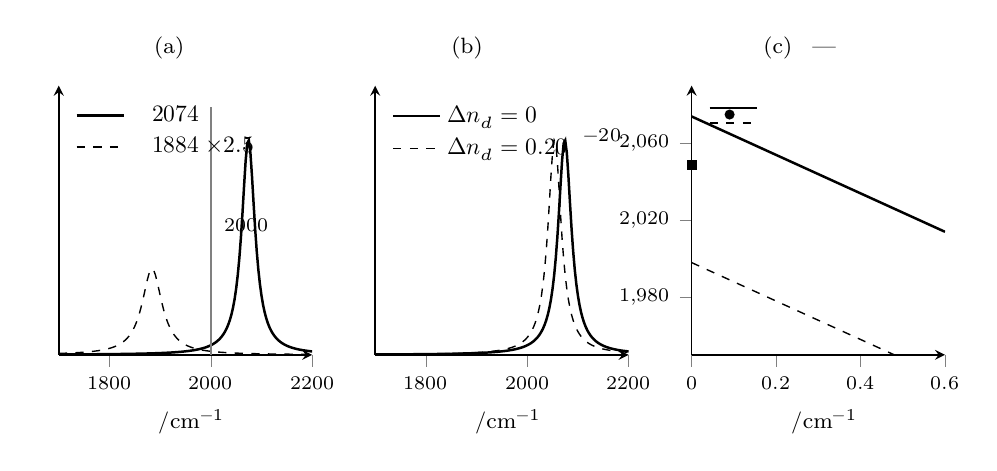
\begin{tikzpicture}
\tikzset{declare function={%
  % 参数名只用单字母，且避开 LaTeX 重音命令（\u、\x、\a 之外的单字母需自查）：
  % 用多字母名（如 \xx）会报 "Missing control sequence inserted"；
  % 用 \u、\x 会被当重音命令展开，报 "ill-formatted floating point number"。
  lgk(\p,\c,\a,\w)=(\a/(1+((\p-\c)/\w)*((\p-\c)/\w)));%
  mtop(\p)=2074-(100*\p);%
  mbr(\p)=1998-(100*\p);}}
\begin{groupplot}[
  group style={group size=3 by 1, horizontal sep=8mm,
               ylabels at=edge left, xlabels at=edge bottom},
  width=48mm, height=5.0cm,
  domain=1700:2200, samples=161,
  xmin=1700, xmax=2200,
  axis lines=left, xmajorgrids=false,
  tick align=outside,
  xlabel={波数$/\mathrm{cm^{-1}}$},
  xlabel style={font={\fontsize{8}{9.5}\selectfont}},
  x tick label style={/pgf/number format/1000 sep={},
                      font={\fontsize{7}{8.5}\selectfont}},
  y tick label style={font={\fontsize{7}{8.5}\selectfont}},
  ylabel style={font={\fontsize{8}{9.5}\selectfont}},
  legend style={font={\fontsize{7}{8.5}\selectfont}, draw=none, fill=none,
                at={(0.03,0.97)}, anchor=north west, cells={anchor=west}},
  ]
  \nextgroupplot[ymin=0, ymax=1.25, ytick=\empty,
                 ylabel={相对吸光度（模型）},
                 title={(a) 吸附构型}, title style={font={\fontsize{8}{9.5}\selectfont}}]
    \addplot[mainline, black]      {lgk(x,2074,1.00,16)};
    \addlegendentry{顶位 $2074$}
    \addplot[thinline, black, dashed] {lgk(x,1884,0.40,24)};
    \addlegendentry{桥位 $1884$（$\times2.5$）}
    \draw[gray] (axis cs:2000,0) -- (axis cs:2000,1.15);
    % 【重叠修正，2026-09-30】$2000$ 原用 anchor=south east 挂在 (1996,1.05)，
    % 与图例第一行 `顶位 2074` 完全压在一起：实测 `位`×`0` 墨迹相交 3.5×4.7 pt、
    % 轮廓交叠 1.078 pt²，另有 `位`×`2`、`2`×`0` 两对，合计 3 对。
    % 图例（实测 x 174—246、y 424—446）压不下来，改把标注移到竖线右侧、
    % 图例下方（该处两条谱线均接近 0，实测空白）。
    \node[anchor=west, font={\fontsize{7}{8.5}\selectfont}]
      at (axis cs:2008,0.60) {$2000$};
  \nextgroupplot[ymin=0, ymax=1.25, ytick=\empty,
                 title={(b) 电子密度（几何不变）},
                 title style={font={\fontsize{8}{9.5}\selectfont}}]
    \addplot[mainline, black]          {lgk(x,2074,1.00,16)};
    \addlegendentry{$\Delta n_{d}=0$}
    \addplot[thinline, black, dashed]  {lgk(x,2074-20,1.00,16)};
    \addlegendentry{$\Delta n_{d}=0.20$}
    % 【重叠修正，2026-09-30】$-20$ 原用 anchor=north east 挂在 (2066,1.22)，
    % 落在图例第二行 `$\Delta n_d=0.20$` 上（实测 `=0`×`−20`）。移到图例右侧空白处。
    \node[anchor=west, font={\fontsize{7}{8.5}\selectfont}]
      at (axis cs:2092,1.02) {$-20$};
  \nextgroupplot[ymin=1950, ymax=2090, ytick={1980,2020,2060},
                 % 必须显式覆盖 group 的 domain=1700:2200：本面板横轴是 0—0.6，
                 % 沿用 1700—2200 的 domain 会报 Dimension too large（实测）。
                 domain=0:0.6, xmin=0, xmax=0.6,
                 title={(c) 位移—电子密度关系},
                 title style={font={\fontsize{8}{9.5}\selectfont}}]
    \addplot[mainline, black, samples=61] {mtop(x)};
    \addlegendentry{顶位（模型）}
    \addplot[thinline, black, dashed, samples=61] {mbr(x)};
    \addlegendentry{桥位（模型）}
    \addplot[only marks, mark=*, mark size=1.5pt] coordinates {(0.09,2075)};
    \addplot[only marks, mark=square*, mark size=1.5pt] coordinates {(0,2049)};
    % 【重叠修正，2026-09-30】这里原有的两行方块注记（`• 组成位移 29 cm⁻¹` /
    % `∘ 覆盖度位移 9 cm⁻¹`）与图例 `桥位（模型）` 相撞：实测 6 对字形墨迹相交
    % （最大 `桥`×`移` 0.903 pt²）。该面板内两条斜线贯穿全幅，注记方块
    % （宽 29 mm、高两行）放在任何位置都与斜线或图例相交；而注记内容与图题
    % 完全重复（图题已给出两个位移数值），故删除，改在图题中指明标记点形状。
\end{groupplot}
\end{tikzpicture}
\caption{CO 探针谱带的模型计算：构型、电子密度与位移的关系}
\label{fig:ch07b-co-model}
\modelmark\ 三幅均为模型计算，不是实验谱。(a) 用洛伦兹型峰形示意顶位与
桥位两条谱带的分区，竖线标出 $2000\;\mathrm{cm^{-1}}$ 这一常用分界，
桥位峰按 $2.5$ 倍放大以便比较峰宽；(b) 只改电子密度、保持覆盖度与峰宽
不变，展示每个电子约 $100\;\mathrm{cm^{-1}}$ 的红移率下
$\Delta n_{d}=0.20$ 对应的 $-20\;\mathrm{cm^{-1}}$ 位移；(c) 横轴为模型设定
的位移标尺（单位相当于「每个电子的 $100\;\mathrm{cm^{-1}}$」），两条直线
是顶位与桥位的位移设定，两个标记点按本书实测量级放置：\textbf{实心圆点}为
组成位移 $29\;\mathrm{cm^{-1}}$、\textbf{实心方点}为覆盖度位移
$9\;\mathrm{cm^{-1}}$。读者应看的是：
(a) 中两峰间距远大于 (b) 中的电子效应位移，故构型归属不正确时，位移
判读会被几何效应完全掩盖；(c) 中两个标记点在横轴上的间距说明，要区分
电子效应与覆盖度效应，两者对应的位移必须在量级上先被分开。局限在于斜率
取自模型设定而非标定实验，绝对位置不用于定量。
\figsrc{峰位分界与两类位移的实测数值据原书 §7.3.2（书内 p.452—453 /
PDF p.471—472）；曲线形式为本节模型设定。}
\end{figure}
\end{crosscheck}

\begin{pitfall}
\textbf{把共吸附位移当纯电子效应。}共吸附分子占据部分吸附位、改变局部
覆盖度，本身就会带来位移；只有像本书那样把多个给电子能力不同的分子
排成序列、看\textbf{排序是否与给电子能力一致}，才能把电子效应从几何
与覆盖度效应中分出来。

\textbf{忽略共吸附分子的自身转化。}给电子分子可能与被测表面发生反应，
受主分子（如 $\ce{HCl}$）可能腐蚀或改性表面。谱带位移报告的是「体系
变化后的结果」，不必然是「该分子给电子」这一单一原因。

\textbf{把「位移量」当「转移电子数」。}图 \ref{fig:ch07b-co-model}(c)
中的直线是模型设定。真实体系中消光系数、偶极耦合与构型分布同时变化，
位移与电子转移量不是一一对应。
\end{pitfall}

\subsection{红外光谱在氧化物与分子筛催化剂表征中的应用}
\label{sec:ch07b-oxide}

\subsubsection{表面羟基的类型与酸强度}

\begin{probout}
要输出的是三件事：表面上存在\textbf{哪几种}结构羟基、每种羟基的\textbf{酸
强度}如何、以及各种羟基的\textbf{可接近程度}（能不能被探针分子接近）。
结构羟基的性质与表面酸性密切相关，而脱水反应、甲酸分解等许多催化反应
又与它直接相关\src{S1 §7.4.2，书内 p.465 / PDF p.484}，所以这三件事是
把红外谱与反应性能关联起来的必经环节。
\end{probout}

\begin{principle}
羟基的振动分析可近似为双中心的非谐振子模型。振动态表示为
\begin{equation}
  G(v)=\omega_{e}\!\left(v+\tfrac{1}{2}\right)
       -\omega_{e}x_{e}\!\left(v+\tfrac{1}{2}\right)^{2},
  \label{eq:ch07b-morse-levels}
\end{equation}
式中 $G(v)$ 为实验测得振动频率（以波数计），$\omega_{e}$ 为简正频率，
$x_{e}$ 为非谐振因子，$v$ 为振动能级数。
对应的 Morse 势能函数为
\begin{equation}
  U(r)=D\left[\,e^{-\beta(r-r_{e})}-1\,\right]^{2},
  \label{eq:ch07b-morse}
\end{equation}
式中 $r_{e}$ 与 $r$ 分别为振动原子的平均距离和瞬间距离，$D$ 为势阱深度，
$\beta$ 为与约化质量、简正频率有关的参数
\src{S1 §7.4.2，书内 p.470 / PDF p.489}。
\tocheck{未对照原页面图像：源 OCR 把 $\beta$ 与 $D$ 的表达式印成
「$\beta=2.48\times10^{7}(\cdots)$」「$D=\cdots$」等残形，本节只写出
可确证的标准 Morse 形式，$\beta$、$D$ 的具体表达式及其常数取值须核
原页 p.470。}
\end{principle}

\begin{principle}
用这套模型可以只靠一对同位素光谱算出解离能。由同一羟基的 OH 与 OD
伸缩振动基频（分别记 $v_{\mathrm{OH}}$、$v_{\mathrm{OD}}$，对应简正频率
$\omega_{\mathrm{H}}$、$\omega_{\mathrm{D}}$），可解出简正频率与非谐振
因子，进而得到质子解离能
\begin{equation}
  D_{0}=\frac{\omega_{e}^{2}}{4\,\omega_{e}x_{e}} .
  \label{eq:ch07b-D0}
\end{equation}
本书指出，羟基的质子解离能（即质子转移活化能）与 B 酸中心的酸性及固体
表面催化性能有密切联系；由吸附前后羟基与氘化羟基谱带的化学位移，可算出
有效质子转移活化能 $D_{\mathrm{eff}}$\src{S1 §7.4.2，书内 p.471 /
PDF p.490}。

\textbf{成立条件}：式 \equref{eq:ch07b-D0} 建立在「吸附分子的主要影响是
增大羟基的非谐振性、而简正频率基本不变」这一近似之上。本书明确指出，
只有在该近似下，才能从一个羟基基振动红外跃迁的化学位移求出质子转移
活化能的降低量；若吸附同时改变简正频率，则须用完整的式
\equref{eq:ch07b-morse-levels} 与 \equref{eq:ch07b-morse} 联立求解。
\tocheck{未对照原页面图像：本书由位移求 $D_{\mathrm{eff}}$ 的中间步骤
（源 OCR 残存「$D_{0}=\cdots/(\omega_{e}-2\omega_{e}x_{e})$」
「$X=(\omega_{e}-\omega_{e}^{*})/2\omega_{e}$」
「$\Delta\omega=\omega_{e}^{*}-\omega_{e}$」等形）无法从文本层可靠重建，
本节只保留式 \equref{eq:ch07b-D0} 与「由位移求活化能降低」这一结论，
中间式须核原页 p.471—472。}
\end{principle}

\begin{obs}
\textbf{二氧化硅表面。}在不同温度下脱水后测红外光谱，可发现吸附水对结构
羟基影响明显。特别的是，$800\,\degC$ 脱水后 $\ce{SiO2}$ 表面结构羟基
出现转动结构（$P$ 支、$R$ 支），表明羟基在 $\ce{SiO2}$ 表面上可以自由
转动，而在其他表面从未发现这一现象\src{S1 §7.4.2，书内 p.466—467 /
PDF p.485—486}。

\textbf{脱水温度与可接近程度。}$473\;\mathrm{K}$ 脱水后的硅溶胶表面，
$3740\;\mathrm{cm^{-1}}$ 处出现一尖谱带，宽谱带在 $3660\;\mathrm{cm^{-1}}$
与 $3550\;\mathrm{cm^{-1}}$；由同位素交换（OH $\to$ OD，
$2740\;\mathrm{cm^{-1}}$ 一带为 OD 伸缩带）结果看出，
$3550\;\mathrm{cm^{-1}}$ 峰与 $3660\;\mathrm{cm^{-1}}$ 峰是不可接近的
\src{S1 §7.4.2，书内 p.467 / PDF p.486}。
\tocheck{未对照原页面图像：源 OCR 作「$3740\;\mathrm{cm^{-1}}$ 峰、
$3550\;\mathrm{cm^{-1}}$、$3660\;\mathrm{cm^{-1}}$ 峰是不可接近的
（$3\cdots0\;\mathrm{cm^{-1}}$ OH 分 $27\cdots00$）」，可接近与不可接近
三种羟基的\textbf{一一对应关系}在文本层残缺，须核原页 p.467 与图 7-53。}

\textbf{氧化铝表面。}$\gamma\text{-}\ce{Al2O3}$ 经严格脱水后，红外光谱中
存在五个不同吸收带，对应五种不同的结构羟基。进一步研究发现各种结构
羟基的电子云密度顺序为 $\mathrm{A}>\mathrm{D}>\mathrm{B}>\mathrm{E}>\mathrm{C}$，
即 A 类部位最负、碱性最强，C 类最正、酸性最强，B 类部位近于中性
\src{S1 §7.4.2，书内 p.468 / PDF p.487}。

\textbf{羟基类型的一般图景。}把上述各体系合起来看，结构羟基可按其与骨架
的连接方式分成三类：\textbf{端式}（单个 $\mathrm{Si}$ 或 $\mathrm{Al}$
上的 $\equiv\!\mathrm{Si{-}OH}$）、\textbf{桥式}（$\equiv\!\mathrm{Si{-}(OH){-}Al}\equiv$
一类跨两个骨架原子的羟基，本书在分子筛处按变角振动单独列出）与
\textbf{巢式}（羟基位于骨架缺陷／空位处，配位环境不完整）。
\textbf{三者的酸强度顺序为端式 $<$ 巢式 $<$ 桥式}，因为桥式羟基所连的
$\mathrm{Al}$ 电负性低于 $\mathrm{Si}$、$\mathrm{Al{-}O}$ 键更长，
$\mathrm{O{-}H}$ 上的电子云密度被拉得更低，质子更易给出；巢式羟基因
配位不完整而处于两者之间。\textbf{请注意本节的证据边界}：源文本明确给出
并可用数据支持的是\textbf{端式与桥式}两类——$\ce{SiO2}$、无定形硅酸铝、
X 型、Y 型、丝光型分子筛都在 $3745\;\mathrm{cm^{-1}}$ 处有
$v_{\mathrm{OH}}$ 带（端式），而桥式羟基的变角振动与端式可相差
$180$—$250\;\mathrm{cm^{-1}}$\src{S1 §7.4.2，书内 p.472—473 /
PDF p.491—492}；「巢式」的命名与上述三者酸强度的\textbf{定量排序}，
源文本只以「可接近／不可接近」与电子云密度顺序间接涉及，未给出该排序
本身。\tocheck{未对照原页面图像：三羟基类型的命名（端式／桥式／巢式）
与「端式 $<$ 巢式 $<$ 桥式」这一酸强度排序，源文本 §7.4.2 未直接写出，
系按固体酸领域的通行分类补入；本书是否采用同一命名与排序须核
书内 p.466—469 / PDF p.485—488。}
\tocheck{未对照原页面图像：源 OCR 中表 7-7 的五种羟基波数只完整保留了
$3800$、$3780$、$3744$、$3733$、$3700$ 五个数，与其类型字母
（A—E）及最近邻配位数的\textbf{对应关系}已错行，此处不逐一列表，
须核原页 p.469。}
\end{obs}

\begin{infer}
由此得到「羟基类型—酸强度」的判读规则：\textbf{同一表面上的羟基并非
等价}，其酸强度由该羟基所处配位环境的电子云密度决定；电子云密度越低
（越缺电子），质子越易给出，酸强度越高。A 类最负故碱性最强、C 类最正
故酸性最强，中间的 B 类近中性，就是这条规则的直接体现。
判读时因此不能把「$3700$ 多波数区的一簇峰」当成一种羟基，也不能把
总羟基量当作酸量。

\textbf{氢键引起的位移。}当羟基与吸附质形成氢键时，羟基伸缩带向低波数
位移、同时强度增加、半宽增大。本书用氢受主化合物（$\ce{C6H6}$、
$\ce{CH3CN}$）吸附后的红外光谱来表征表面羟基的酸性强度：由键合作用引起
的羟基伸缩吸收带的\textbf{化学位移}可估计有关 OH 基的酸性，并可识别
表面 OH 的类型\src{S1 §7.4.2，书内 p.469 / PDF p.488}。
在含 $75\%$ $\ce{SiO2}$ 的 $\ce{SiO2{-}Al2O3}$ 上，吸附受主化合物后，
$3750\;\mathrm{cm^{-1}}$ 一带发展成两个峰，说明表面存在两种 OH：
一种构型为 $\equiv\!\mathrm{Si{-}OH}$，类似于纯 $\ce{SiO2}$ 表面；
另一种为 $\equiv\!\mathrm{Al{-}(OH){-}Si}\equiv$，其酸性较强，类似于
硅被 $\ce{Al^{3+}}$ 取代后的桥式羟基\src{S1 §7.4.2，书内 p.469 /
PDF p.488}。\textbf{位移的幅度即酸强度的量度}，这是把「位置」用于
强度判断的少数几处之一，成立前提是探针分子的碱性已知且同一批实验内
一致。
\end{infer}

\begin{crosscheck}
\textbf{用近红外组频带把「看不清的分辨开」。}由于强烈的本底，羟基变形
振动（$700$—$1100\;\mathrm{cm^{-1}}$）的信息过去一直无法获得。用近红外
方法考察分子筛的基频、倍频和组频后，可由羟基伸缩振动 $v_{\mathrm{OH}}$
与变角振动 $\delta_{\mathrm{OH}}$ 的组频 $(v+\delta)$、以及伸缩振动基频，
通过下式求出变角振动频率 $\delta_{\mathrm{OH}}$
\begin{equation}
  (v+\delta)=v_{\mathrm{OH}}+\delta_{\mathrm{OH}}-2X_{1},
  \label{eq:ch07b-combination}
\end{equation}
式中 $X_{1}$ 为两振动模式的相互作用系数，本书指出对分子筛而言它与
$\ce{SiO2}$ 的值相近\src{S1 §7.4.2，书内 p.472 / PDF p.491}。
\tocheck{未对照原页面图像：源 OCR 把式（7-11）印成
「嘿$=$嘿$+$嘿$+$嘿」一类的重复字形，$X_{1}$ 的系数（$2X_{1}$ 还是
$X_{1}$）及其数值量级在文本层无法判定；本节按「组频 $=$ 两个基频之和
减去相互作用项」的标准形式重建，须核原页 p.472。}

这一手段的价值在于\textbf{灵敏度}：$\ce{SiO2}$、无定形硅酸铝、X 型、
Y 型、丝光型分子筛都在 $3745\;\mathrm{cm^{-1}}$ 处有一个 $v_{\mathrm{OH}}$
吸收带，靠基频无法区分；但它们的 $\delta_{\mathrm{OH}}$ 明显不同，
桥式羟基与端式羟基的变角振动可相差 $180$—$250\;\mathrm{cm^{-1}}$。
更直接的例子是：X 型分子筛在桥式羟基基频区只有一个 $3650\;\mathrm{cm^{-1}}$
吸收带，而在组频带却分别在 $4650$ 与 $4690\;\mathrm{cm^{-1}}$ 出现两条，
表明该区存在两种羟基，但在基频范围无法分辨
\src{S1 §7.4.2，书内 p.472—473 / PDF p.491—492}。结论是：
\textbf{变角振动对羟基周围环境变化的灵敏度大于伸缩振动基频}，故基频
分不开时应当回查近红外组频带。
\tocheck{未对照原页面图像：源 OCR 中表 7-11 的端基／桥式羟基行大量损坏
（端基 $\mathrm{Si{-}OH}$ 的 $\delta$ 值残存 $795$、$820$、$805$、$825$
等数，桥式羟基行残存 $835$ 等数），各分子筛与各羟基类型的
$v+\delta$ 与 $\delta$ 一一对应关系须核原页 p.472—473。}

\textbf{用同位素交换独立验证。}$\ce{SiO2}$、$\ce{Al2O3}$、
$\ce{SiO2{-}Al2O3}$ 表面羟基与 $\ce{CD4}$ 的交换能力与酸性\textbf{没有}
直接关系——$\ce{SiO2}$ 上羟基中的质子最难交换
\src{S1 §7.4.2，书内 p.470 / PDF p.489}。这一条是对「酸性强则质子活泼」
这一直觉的反例：判断可接近性必须另做同位素实验，不能由酸强度外推。
\end{crosscheck}

\subsubsection{固体表面酸性（L 酸与 B 酸）的测定}

\begin{principle}
需要测定的是表面酸性位的\textbf{类型}（L 酸／B 酸）、\textbf{强度}与
\textbf{酸量}三者。碱滴定法、碱性气体吸附法、热差法等都不能区分 L 酸
部位与 B 酸部位，红外光谱法则可以有效区分
\src{S1 §7.4.3，书内 p.474 / PDF p.493}。
区分依据是探针分子在两类位上的\textbf{成键方式不同，因而环变形振动的
位置不同}：吡啶以氮的孤对电子配位到 L 酸部位，保持中性分子形式；在
B 酸部位则被质子化生成吡啶阳离子 $\mathrm{PyH^{+}}$。二者在
$1400$—$1700\;\mathrm{cm^{-1}}$ 的环变形振动区给出不同的谱带组合。
归属位置与抽空条件汇总于 \tabref{tab:ch07b-py}。
\end{principle}

\begin{table}[htbp]
\centering
\caption{吡啶吸附物种的环变形振动归属与抽空条件}
\label{tab:ch07b-py}
\small
\begin{tabularx}{\onecolwidth}{@{}>{\raggedright\arraybackslash}p{26mm}
 >{\raggedright\arraybackslash}p{34mm}
 >{\raggedright\arraybackslash}X@{}}
\toprule
吸附形式 & 归属谱带$^{\mathrm{a}}$ & 抽空行为与判读要点 \\
\midrule
物理吸附吡啶 &
 约 $1445$（$19b$）、约 $1490$（$19a$） &
 室温即可抽除；与氯仿溶液中的纯吡啶谱对应。测化学吸附物种时必须用
 $150\,\degC$ 抽空把它扣掉 \\
氢键吸附的吡啶 &
 约 $1450$（$19b$）、约 $1490$（$19a$） &
 $150\,\degC$ 可抽除。$19b$ 位置与 L 酸位配位吡啶几乎重合，
 不能单独用它下结论 \\
L 酸位配位吡啶 &
 \textbf{约 $1450$}（$19b$）、约 $1490$（$19a$） &
 室温抽空后保留，须 $150\,\degC$ 以上才逐步脱除；
 $1450$ 带是 L 酸位的判据带 \\
B 酸位质子化吡啶（$\mathrm{PyH^{+}}$） &
 \textbf{约 $1540$}（$19b$）、约 $1490$（$19a$） &
 强吸附，抽空至 $420\,\degC$ 仍可保留；$1540$ 带是 B 酸位的判据带。
 质子化产生的其他谱带位置受氢键影响变化大，不作定量依据 \\
两类位共有 &
 约 $1490$（$19a$） &
 \textbf{不能用它区分 L 酸与 B 酸}，只能用来说明「存在酸位」 \\
\bottomrule
\end{tabularx}

\vspace{1pt}
{\srcsize $^{\mathrm{a}}$ 单位 $\mathrm{cm^{-1}}$；$19b$、$19a$ 为环变形
振动的模式记号。数值为文献通行归属值，不同文献间可有约
$10\;\mathrm{cm^{-1}}$ 的差异，比对时须用同一套文献值。}
\tocheck{未对照原页面图像：本书表 7-12（书内 p.475 / PDF p.494）在源 OCR
中列间错位严重——$19b$ 与 $19a$ 两列的数被拆到不同行，「$1457$」
「$1625$」「$1615$」「$1540$」等数各自所属的吸附形式无法从文本层判定；
本表只列出源文本与正文别处可相互印证的带位，其余带位与全部
\textbf{最近邻配位数、峰半宽}数据一律不列，须核原页 p.475 后补齐。}
\end{table}

\begin{measure}
条件设置中三件事决定成败：
\textbf{(1) 探针碱性决定分辨能力。}本书指出，吡啶的碱性弱于 $\ce{NH3}$，
它能同弱酸部位反应\src{S1 §7.4.3，书内 p.474 / PDF p.493}；
反过来，$\ce{NH3}$ 碱性过强，会把强、弱酸位一并滴定，从而掩盖弱酸位的
差异。
\textbf{(2) 必须扣除物理吸附与气相。}为排除物理吸附吡啶的影响，应在
吸附后再于 $150\,\degC$ 下抽空，然后测定红外光谱
\src{S1 §7.4.3，书内 p.475 / PDF p.494}。物理吸附物种在室温即可抽除，
因而「室温吸附」与「$150\,\degC$ 抽空后」两张谱的差，就是化学吸附物种。
\textbf{(3) 选对用于定量的谱带。}吡啶分子面内环变形振动在若干位置出现，
但并非每条都适合定量（见下文误判）。
\end{measure}

\begin{obs}
\textbf{参比体系。}在氯仿溶液中：纯吡啶谱相当于物理吸附态；吡啶与典型
电子对受体 $\ce{BH3}$ 形成的 $\mathrm{C5H5N{+}{-}BH3}$ 相当于吸附在
L 酸部位；吡啶与 $\ce{HCl}$ 形成的 $\mathrm{C5H5N{+}HCl}$（即
$\mathrm{PyH^{+}}$ 与 $\mathrm{Cl^{-}}$）相当于吸附在 B 酸部位
\src{S1 §7.4.3，书内 p.474 / PDF p.493}。
\tocheck{未对照原页面图像：源 OCR 把该参比谱图 7-58 的谱带数值大量丢失
（仅残存 $1465$、$1585$、$1610$、$1640$ 等零散数与
「$1520\;\mathrm{cm^{-1}}$ 的宽峰由溶剂氯仿引起」一句），三个参比物种
各自的完整谱带列表须核原页 p.474 与图 7-58。}

\textbf{表面酸性测定的实例。}
$\ce{SiO2}$：吡啶在其上只是物理吸附，$150\,\degC$ 抽空后几乎全部脱附，
进一步表明纯 $\ce{SiO2}$ 上没有酸性中心。
$\ce{Al2O3}$：只能看到 L 酸中心（$1450\;\mathrm{cm^{-1}}$），看不到
B 酸中心。
$\ce{SiO2{-}Al2O3}$：在 $1600$—$1450\;\mathrm{cm^{-1}}$ 范围内除
$1450\;\mathrm{cm^{-1}}$ 的 L 酸带外，还出现 $1540\;\mathrm{cm^{-1}}$
的 B 酸带，说明该表面同时存在 L 酸部位与 B 酸部位；引入少量
$\ce{H2O}$ 后，吸附在 B 酸部位（$1540\;\mathrm{cm^{-1}}$）的吡啶浓度
增加，而 L 酸部位（$1450\;\mathrm{cm^{-1}}$）的浓度减少
\src{S1 §7.4.3，书内 p.475—476 / PDF p.494—495}。
由该体系还可读出四条更细的结论：表面至少存在三种 L 酸部位，其中一种
与混合相有关（加水可转变成 B 酸），另外两种一强一弱与 $\ce{Al2O3}$ 相
有关（加水不能转变成 B 酸）；随 $\ce{Al2O3}$ 含量增加，L 酸部位增加，
且主要是增加弱酸部位；混合相增加时强酸部位增加
\src{S1 §7.4.3，书内 p.476 / PDF p.495}。
\end{obs}

\begin{infer}
\textbf{L／B 归属的读法}：认定某样品有 B 酸位，依据是
$1540\;\mathrm{cm^{-1}}$ 带的出现，它对应质子化物种 $\mathrm{PyH^{+}}$
的环变形振动；认定有 L 酸位，依据是 $1450\;\mathrm{cm^{-1}}$ 带，它对应
以配位键结合的中性吡啶。必须同时看这两条带，因为它们不是同一条带的位移，
而是两个不同物种的谱带；只看一条带无法判断另一类酸位是否存在。
$1490\;\mathrm{cm^{-1}}$ 一带为两类位共有，因此\textbf{不能用它区分}
L 酸与 B 酸。

\textbf{「加水使 L 酸转成 B 酸」的含义}：$1540$ 带增强而 $1450$ 带减弱，
说明水把一部分 L 酸部位转化成了能给出质子的 B 酸部位，而不是简单地把
探针分子洗掉。这一现象把「酸位类型」与「预处理／含水状态」绑定在一起，
因此酸位类型的报告必须同时报告预处理条件。

\textbf{$\ce{NH3}$ 作为探针的归属}：$\ce{NH3}$ 吸附在 L 酸部位时以氮的
孤对电子配位，其红外光谱类似于金属离子与 $\ce{NH3}$ 的配位络合物；
在 B 酸部位则生成 $\mathrm{NH4^{+}}$。本书给出的区分主要依靠
$\delta_{\mathrm{N{-}H}}$ 变形振动：B 酸位与 L 酸位分别在
$1432\;\mathrm{cm^{-1}}$ 与 $1610\;\mathrm{cm^{-1}}$ 一带给出谱带
\src{S1 §7.4.3，书内 p.476—477 / PDF p.495—496}。注意该归属表引自
文献，不同文献的数值有约 $10\;\mathrm{cm^{-1}}$ 的差异，故比对时须用
同一套文献值。
\end{infer}

\begin{pitfall}
\textbf{误判一：把 $1490\;\mathrm{cm^{-1}}$ 带当 L 酸或 B 酸的判据。}
该带为两类位共有，用它判断酸位类型会把「有无酸位」错读成「有哪类酸位」。

\textbf{误判二：不扣物理吸附与气相就报酸量。}扣除的前提是有明确的抽空
温度阈值。本书的做法是吸附后在 $150\,\degC$ 抽空再测
\src{S1 §7.4.3，书内 p.475 / PDF p.494}。若省略这一步，室温可抽除的
物理吸附吡啶会计入 B 酸或 L 酸量；若抽空温度过高，部分弱酸位上化学
吸附的探针也会脱附，酸量被低估。此外，吡啶在强酸位上的质子化产物本身
就是被测物种，探针的自身反应与测量对象不可分离。

\textbf{误判三：用 $\nu(\mathrm{N{-}H})$ 带表征 B 酸量。}由于该带受
氢键等因素影响变化大、不易确定，本书明确指出一般不用它表征 B 酸部位
\src{S1 §7.4.3，书内 p.475 / PDF p.494}。

\textbf{误判四：跨样品直接比强度。}不同样品自支撑片的厚度与散射本底
不同，方程 \equref{eq:ch07b-beer} 中的 $l$ 不可比。跨样品比较须做厚度
归一或以内标带归一（见 \S\,\ref{sec:ch07b-oxide} 前文的说明）。

\textbf{误判五：用碱性过强的探针找弱酸位。}$\ce{NH3}$ 会把强、弱酸位
同时滴定，掩盖弱酸位的差异；要分辨弱酸位应改用碱性较弱的探针
（如吡啶），必要时再配合不同尺寸的探针区分孔内与外表（见下文）。
\end{pitfall}

\begin{crosscheck}
\textbf{用探针分子尺寸区分「孔内」与「外表面」。}酸中心的\textbf{空间
分布}是另一个必须回答的问题，靠的是不同截面积的探针分子。吡啶的临界
直径在 $6\;\mathrm{\text{\AA}}$ 左右，测得的是\textbf{总的}酸中心
（含介孔与微孔表面）；$2,6-$二甲基吡啶的临界直径更大，只能接近外表面
及孔口附近较大的中心。本书对系列样品（介孔硅铝与不同结晶度的 ZSM-5）
比较后给出：$2,6-$二甲基吡啶可接近的 B 酸中心数与外表面 B 酸所占
百分比顺序为 $\mathrm{Al{-}Meso}<\mathrm{UL{-}ZSM{-}5{-}2}
<\mathrm{UL{-}ZSM{-}5{-}4}<\mathrm{ZSM{-}5}$
\src{S1 §7.4.3，书内 p.481 / PDF p.500}。
\tocheck{未对照原页面图像：$2,6-$二甲基吡啶的临界直径数值在源 OCR 中
作「11.5 人$^{2}$」，量纲（面积还是直径）与数值均须核原页 p.481。}

\textbf{用羟基带与吡啶带的对应关系交叉验证。}分子筛上可同时看到两种
结构羟基，其中 $3612\;\mathrm{cm^{-1}}$ 一带的羟基对应于吡啶吸附在其上
产生的 B 酸 $1540\;\mathrm{cm^{-1}}$ 带；用大尺寸探针后该羟基带与
$1540$ 带同时消失，进一步证明此中心存在于微孔内
\src{S1 §7.4.3，书内 p.481 / PDF p.500}。这种「羟基带与探针带成对
消失」的验证，比单独看 $1540$ 带可靠。

\textbf{用改性实验验证归属。}用沸石骨架振动谱带作内标的计算机红外
差谱方法发现：P 改性 HZSM-5 时，P 的主要作用是「杀掉」大部分强的
B 酸中心（位于 $3611\;\mathrm{cm^{-1}}$ 位置的羟基）；Mg 改性除「杀掉」
大部分强 B 酸中心外，还形成一部分 L 酸中心
\src{S1 §7.4.3，书内 p.478 / PDF p.497}。把这一结果与 $\ce{NH3}$ 的
TPD（HZSM-5 表面存在强、弱两类酸性中心，P 和 Mg 改性后强酸部位大为
减少）以及 ESCA 的表面组成结果相对照，三条独立证据指向同一结论，这种
「红外差谱 $+$ TPD $+$ 表面组成」的组合是酸位表征的常规回查方式。

\textbf{补充的探针物性参照。}本书表 7-16 列出部分胺类探针的碱度
（$\mathrm{p}K_{a}$）与临界直径供选择探针时参考
\src{S1 §7.4.3，书内 p.480 / PDF p.499}。
\tocheck{未对照原页面图像：该表在源 OCR 中列错行严重——同一分子
$\mathrm{C6H5N}$（吡啶）出现两次且记为「$5.21$」与「$11.12$」两个
相差甚远的 $\mathrm{p}K_{a}$，$\mathrm{C6H5NH2}$ 记为「$0.46$」，
而氨与水溶液中氨的标准 $\mathrm{p}K_{a}$ 为 $9.25$ 而源文正文作
「5」。故本表数值\textbf{一律不引用}，须核原页 p.480 后方可使用。}
\end{crosscheck}

\subsubsection{氧化物表面氧物种与低碳烃活化}

\begin{principle}
甲烷是烃类中组成最简单、对称性最高、化学上最惰性的分子，在常温下与
催化剂表面相互作用时间非常短暂，很难直接观察到它在表面的活化过程。
另一方面，碱性氧化物表面存在一层稳定的碳酸盐，去除这一保护层很困难，
使表面氧物种的研究很少进行\src{S1 §7.4.4，书内 p.483 / PDF p.502}。
要突破这两点，实验上必须走「\textbf{先净化表面、再低温捕集}」的路线：
在 $1000\;\mathrm{K}$ 以上用纯 $\ce{O2}$ 长时间处理以去除表面碳酸盐
保护层，随后骤冷至 $173\;\mathrm{K}$ 进行氧物种和甲烷吸附态的红外
光谱研究，并与化学捕集技术、同位素交换技术结合
\src{S1 §7.4.4，书内 p.484 / PDF p.503}。

\textbf{判据的原理}：甲烷的 $v_{1}$ 对称伸缩振动在气相中是红外无活性的
（Raman 活性）。若分子以降低对称性的方式吸附在表面上，该振动会变为
红外活性并出现位移——\textbf{「对称性下降」由红外活性出现来判定，
「活化程度」由位移量来判定}。这是本节所有归属的共同基础。
\end{principle}

\begin{obs}
\textbf{氧物种。}经 $1000\;\mathrm{K}$ 纯 $\ce{O2}$ 长时间处理并抽高真空
得到洁净的 $\ce{CeO2}$ 表面，骤冷至 $210\;\mathrm{K}$ 吸附
$^{16}\ce{O2}$ 后的红外光谱中，$1128\;\mathrm{cm^{-1}}$ 谱带被归属为
$\ce{O2^{-}}$ 物种；再用 $^{18}\ce{O2}$ 作同位素实验，由同位素位移
进一步确认 $1065\;\mathrm{cm^{-1}}$ 谱带为 $\ce{O2^{2-}}$ 物种。
这一结果表明在新鲜的 $\ce{CeO2}$ 表面至少存在两种氧物种
\src{S1 §7.4.4，书内 p.485 / PDF p.504}。
\tocheck{未对照原页面图像：源 OCR 把 $1128\;\mathrm{cm^{-1}}$ 与
$1065\;\mathrm{cm^{-1}}$ 两条谱带各自归属的物种名印成「$^{16}\ce{O2^{-}}$」
与「$^{18}\ce{O2^{2-}}$」等混形，两个归属与两种氧物种（超氧
$\ce{O2^{-}}$ 与过氧 $\ce{O2^{2-}}$）的\textbf{一一对应关系}须核
原页 p.485 与图 7-71。}

\textbf{甲烷吸附态。}新鲜的 $\ce{CeO2}$ 表面上甲烷低温吸附后，在
$2875\;\mathrm{cm^{-1}}$ 出现吸收带；而气相 $\ce{CH4}$ 的
$v_{1}$ 在 $2917\;\mathrm{cm^{-1}}$ 处（Raman）并无红外活性。即：
甲烷吸附在 $\ce{CeO2}$ 表面导致 $\mathrm{C{-}H}$ 键振动由 Raman 活性
变为红外活性（对称性下降），并且与自由 $\ce{CH4}$ 分子相比存在
$42\;\mathrm{cm^{-1}}$ 的化学位移，表明甲烷分子被活化
\src{S1 §7.4.4，书内 p.485—486 / PDF p.504—505}。
不同氧化物上的位移量不同：$\ce{CeO2}$ 上约 $42\;\mathrm{cm^{-1}}$，
$\ce{MgO}$ 上 $17\;\mathrm{cm^{-1}}$，$\ce{Al2O3}$ 上
$27\;\mathrm{cm^{-1}}$\src{S1 §7.4.4，书内 p.486 / PDF p.505}。

\textbf{晶面对吸附的影响。}用 CO 探针研究 $\ce{CeO2}$ 单晶表面氧缺陷的
化学活性时发现：CO 在理想 $\ce{CeO2}(111)$ 晶面的红外振动峰位于
$2154\;\mathrm{cm^{-1}}$，而在还原表面的峰位于 $2163\;\mathrm{cm^{-1}}$；
CO 在缺陷位的红外峰显示出很小的波数变化，远远小于原来的预期，且
\textbf{不同于 $\ce{TiO2}$ 等材料上缺陷位吸附红移的现象}。借助理论计算
归属后认为，$2154\;\mathrm{cm^{-1}}$ 的峰来源于紧邻缺陷的六配位
$\ce{Ce^{3+}}$ 上吸附的 CO，而非离氧缺陷更远处的七配位 $\ce{Ce^{3+}}$
\src{S1 §7.4.5，书内 p.486—487 / PDF p.505—506}。
\end{obs}

\begin{infer}
\textbf{位移—活化程度的读法}：$42\;\mathrm{cm^{-1}}$（$\ce{CeO2}$）
$>27\;\mathrm{cm^{-1}}$（$\ce{Al2O3}$）$>17\;\mathrm{cm^{-1}}$
（$\ce{MgO}$）这一顺序，说明同一探针分子（甲烷）在不同氧化物表面上被
活化的程度不同；位移越大表示 $\mathrm{C{-}H}$ 键被削弱得越多。因此
\textbf{「位移量」在这里被用作活化程度的相对标尺}，比较必须在同一探针、
同一吸附温度下进行。

\textbf{配位数而非距离决定吸附位置}：$\ce{CeO2}$ 上 CO 在缺陷位的位移
\textbf{很小}，与 $\ce{TiO2}$ 等材料上缺陷位吸附\textbf{红移}的常见
现象相反。理论计算给出的解释是：该峰来自紧邻缺陷的六配位
$\ce{Ce^{3+}}$，而非更远处的七配位 $\ce{Ce^{3+}}$。由此得到的判读
规则是——\textbf{氧化物的配位结构（配位数）在表面化学相互作用中起
决定性作用}，不能仅凭「离缺陷的距离」推断吸附位与位移方向
\src{S1 §7.4.5，书内 p.486—487 / PDF p.505—506}。这一结论与本书对
甲氧基的研究相互印证：甲氧基 $\mathrm{C{-}O}$ 键伸缩振动峰的红移与
甲氧基氧原子配位的 Ce 阳离子数\textbf{不存在直接关系}
\src{S1 §7.4.5，书内 p.487 / PDF p.506}——即不能用「配位数越多红移越大」
这类单因素规则去套。
\end{infer}

\begin{pitfall}
\textbf{误判一：把位移单因素归因于电子效应或配位数。}本书用两处实测
反例说明这一点：$\ce{CeO2}$ 缺陷位 CO 的位移小于预期且方向与
$\ce{TiO2}$ 相反；甲氧基 $\mathrm{C{-}O}$ 红移与配位 Ce 阳离子数无直接
关系。凡遇到「位移不符合预期」的情形，正确做法是补做同位素实验与理论
计算，而不是修改归属规则去迁就数据。

\textbf{误判二：不区分「对称性下降」与「化学位移」两个信息来源。}
$v_{1}$ 由 Raman 活性变为红外活性只证明吸附降低了对称性；键被削弱的
程度必须另由位移量判断。把二者混为一谈会把「分子被表面固定住」误读成
「分子被活化」。

\textbf{误判三：忽略表面碳酸盐保护层。}碱性氧化物表面天然覆盖一层稳定
碳酸盐，不去除就直接做吸附实验，测到的主要是碳酸盐的变化而不是氧物种
与烃的相互作用。去除条件（$1000\;\mathrm{K}$ 以上纯 $\ce{O2}$ 长时间
处理）本身就是这套实验的关键条件，不能省略。

\textbf{误判四：把低温吸附态当成反应条件下的真实中间物。}$173\;\mathrm{K}$
骤冷下捕集到的吸附态是\textbf{稳定化}的观察对象；从它推断反应条件下的
活化路径，需要另有证据（如升温过程中的谱带演化、同位素标记实验）。
\end{pitfall}

\begin{crosscheck}
\textbf{同位素交换是归属的第一道回查。}氧物种的归属靠
$^{16}\ce{O2}/^{18}\ce{O2}$ 的同位素位移确认；甲烷吸附态的归属靠
$\ce{CD4}$ 同位素实验与同 CO 共吸附的双分子探针方法证实
\src{S1 §7.4.4，书内 p.486 / PDF p.505}。凡涉及含氧或含氢物种的归属，
同位素位移应当与位置归属同时报告。

\textbf{双分子探针是电子转移方向的回查。}用 CO 共吸附观察
$v_{\mathrm{CO}}$ 的位移方向（见 \S\,7.3.3 的读图实例），可以判断吸附
过程中电子转移的方向与程度，这一手段与氧物种的红外归属互为补充
\src{S1 §7.3.3，书内 p.457 / PDF p.476}。

\textbf{分子筛体系的回查逻辑可以照搬。}原位红外与拉曼光谱结合、X 射线
衍射与红外光谱结合，是把「纯相的谱」与「实际催化剂的谱」对应起来的
通行做法：本书用柠檬酸法在较低焙烧温度下获得较大比表面的
V—Mg—O 三种纯相（偏钒酸镁 $\ce{MgV2O6}$、正钒酸镁 $\ce{Mg3V2O8}$、
$\alpha\text{-}\ce{Mg2V2O7}$），由 X 射线衍射、红外光谱和拉曼光谱三者
的对应关系分辨纯相，再与实际催化剂的结果相对照
\src{S1 §7.4.1，书内 p.462—463 / PDF p.481—482}。同理，分子筛骨架振动
可用于测 Si/Al 值并对结构变化敏感——随 Si/Al 值减小，力常数减小、
波数降低；约 $1230\;\mathrm{cm^{-1}}$ 与约 $550\;\mathrm{cm^{-1}}$ 的
谱带对 ZSM-5 的结构变化敏感，约 $1230\;\mathrm{cm^{-1}}$ 谱带的化学
位移同 ZSM-5 的 Si/Al 比呈直线关系，这给出一条用红外测定分子筛 Si/Al
值的途径\src{S1 §7.4.1，书内 p.464—465 / PDF p.483—484}。
\textbf{回查规则}：凡要用一条谱带的位移去标定组成或结构参数，必须先有
X 射线衍射等独立手段确认「结构确实按该参数单调变化」。
\tocheck{未对照原页面图像：源 OCR 中表 7-6（焙烧温度对 ZSM-5 骨架振动
的影响）与图 7-49（$1230\;\mathrm{cm^{-1}}$ 谱带位置与 Si/Al 比的关系）
的数据格全部为空或残形，斜率与拟合式无法读出；本段只保留「成直线关系」
这一定性结论，定量关系须核原页 p.464—465。}
\end{crosscheck}

\begin{srcnote}
\S 7.3 据原书 §7.3（书内 p.448—458 / PDF p.467—477）：探针分子的判读
链条、双探针法测表面组成、几何效应与电子效应、吸附分子相互作用；
\S 7.4 据原书 §7.4.2—7.4.4（书内 p.465—488 / PDF p.484—507）：
表面羟基、固体表面酸性、氧化物表面氧物种与低碳烃活化，另从 §7.4.1
（书内 p.462—465 / PDF p.481—484）取分子筛骨架振动一条用于回查。
表 \ref{tab:ch07b-probes} 的谱带位置取自原书 §7.4.3 的归属
（书内 p.475、p.477 / PDF p.494、p.496）与 §7.4.2 的羟基与碳酸盐数据；
吡啶、$\ce{NH3}$ 的位置为文献归属值，不同文献间有约
$10\;\mathrm{cm^{-1}}$ 的差异。图 \ref{fig:ch07b-co-model} 为本节模型
计算，不是原书图，其峰位分界与两类位移的实测数值取自 §7.3.2。
原书 §7.2「吸附分子的特征和它的红外光谱诊释」属分片 a 范围，本节只在
判读链条处引用其结论。凡源 OCR 失真、未能对照原页面图像重建的公式、
数值与一一对应关系，已就地用 \tocheck{} 标出。
\end{srcnote}
}{}
\IfFileExists{chapters/parts/ch07-c.tex}{% ================================================================
% chapters/parts/ch07-c.tex —— 第 7 章 原位红外光谱方法（分片 c）
% 覆盖：原书 §7.5（加氢精制催化剂活性相与助剂作用，硫化物催化剂）
%        §7.6（原位红外应用于反应机理研究，含光催化水氧化）
%        以及 §7.6 之后的「电化学／光电催化原位红外」部分
%        书内 p.489—518 / PDF p.508—537
% 注：源文本前 93 行（书内 p.489 上的图 7-77、图 7-78，甲烷在 Zn-ZSM-5 上的
%     解离吸附）属 §7.4 的收尾，归分片 b 的范围，本分片不重复。
% 版式自查（WRITER_BRIEF §7.3，单栏版心 165 mm；\onecolwidth ≈ 132 mm）：
%   图 \ref{fig:ch07c-transient}：groupplot 两列，2×54 + 8 = 116 mm，
%     加左侧轴标签与刻度约 13 mm → ≈129 mm ≤ 165 mm  ✓
%   表 \ref{tab:ch07c-probe}、\ref{tab:ch07c-criteria}、\ref{tab:ch07c-formate}
%     均用 tabularx 定宽 \onecolwidth，无「定宽 p{} 凑总宽」。不用 xltabular。
%   declare function 的参数只用 \p（避开 \x、\u），函数体乘法全部加括号；
%     groupplot 不给公共 domain，逐面板显式给 domain，避免 Dimension too large。
% ================================================================

\subsection{加氢精制催化剂活性相与助剂作用（硫化物催化剂）}
\label{sec:ch07c-sulfide}

加氢精制是炼油工业的四大支柱工艺之一。其催化剂牌号有上百种，但大部分是
Co、Mo、Ni、W 的不同组合，工业催化剂载体大多为 \ce{Al2O3}，而使用状态
\emph{均为硫化物}\src{S1 §7.5，书内 p.489 / PDF p.508}。围绕活性相与助剂
作用，文献提出了多个模型（如 CoMoS 相模型与协同作用模型），长期争论不休；
本书作者点出的主要原因是\textbf{原位信息不多}\src{S1 §7.5.4，书内 p.493 /
PDF p.512}。这正是原位红外在这个体系上的位置：它不是给出「催化剂是什么」，
而是在工作状态下给出「有几类可被探针分子接近的中心、助剂改变了哪一类」。

\begin{probout}
本节要输出三件事：①表面上存在哪几类\textbf{配位不饱和中心}（coordinatively
unsaturated site，CUS），各自是什么价态与配位状态；②助剂（Co、Ni、Ru）
改变的是\emph{哪一类}中心的数目或电子状态；③这些改变怎样与加氢脱硫（HDS）、
加氢脱氢（HDY）活性对应起来。要注意的是，红外能可靠给出的是「中心类型」
与「中心的相对变化」；中心数目的绝对值必须由滴定实验（化学吸附或探针分子
饱和吸附）标定后才能谈，否则强度只能读成相对量。
\end{probout}

\subsubsection{硫化物表面在红外测量中的三个特殊问题}

硫化物催化剂的谱学行为与氧化物催化剂有实质差别，读谱前必须先处理这三件事，
否则得到的是「强度失真后的假变化」。

\paragraph{（1）全谱区吸收与散射使基线不稳。}硫化态的 Co--Mo 或 Ni--Mo
催化剂外观为黑色，在可见—红外区有很强的电子吸收；样品的散射又随粒径、
压片或装样方式改变。透射测量中，样品自身吸收与散射把光耗掉，谱带信噪比低、
基线随波数漂移；漫反射测量则要先做 Kubelka--Munk 变换才能把反射率变成与
浓度近似成线性的量
\begin{equation}
  F(R_{\infty})=\frac{(1-R_{\infty})^{2}}{2R_{\infty}}=\frac{K}{S},
  \label{eq:ch07c-km}
\end{equation}
式中 $R_{\infty}$ 为半无限厚样品的漫反射比，$K$ 为吸收系数，$S$ 为散射系数。
\textbf{适用条件是变换成立的前提}：样品必须足够厚（光未穿透）、且在所比较的
谱段内 $S$ 近似不变。硫化物样品粒径分布宽，硫化度改变时表面硫覆盖度也改变，
$S$ 并非常数，故 $F(R_{\infty})$ 的变化里混有散射项。可行的做法是在同一张谱
内取带强度比（例如 $A_{2072}/A_{1694}$），不跨样品比绝对强度。
\tocheck{未对照原页面图像：硫化物自吸收与散射的这段讨论源文未展开，本段按
红外反射光谱的通用处理（Kubelka--Munk 变换及其适用条件）补充，
式~\eqref{eq:ch07c-km} 为学科标准形式，未与原书符号约定逐字核对。}

\paragraph{（2）自吸收与强吸收带附近的谱带失真。}当吸收系数在某个波数附近
出现极大（强吸收带、Reststrahlen 带与 Christiansen 效应所在的波数区间），
颗粒内部的折射与散射会同时变化，谱带的位置和形状都会畸变：带可能变成
不对称，甚至出现表观位移。硫化物在低波数区（骨架与 \ce{Mo-S} 相关振动）
吸收很强，恰是这类畸变最严重的地方。因此报告低波数带位置时，必须同时给出
样品稀释比例与装样方式，并且用同一批装样的谱做相互比较。

\paragraph{（3）羟基与硫醇基必须区分。}硫化后的表面同时存在残余
O--H 与 S--H 两类基团：O--H 伸缩在 $3400$—$3700\;\mathrm{cm^{-1}}$
（游离羟基更高、氢键羟基更低，且随脱水前处理位移），S--H 伸缩在
$2550$—$2600\;\mathrm{cm^{-1}}$，位置分得很开；真正的困难在于
\textbf{S--H 带很弱}——S--H 的偶极变化小，消光系数远低于 O--H，容易被噪声
或水汽、\ce{CO2} 的干扰带淹没。判据是两条：①用 D 交换（\ce{D2} 或
\ce{D2S} 处理）复测，\ce{X-H} 带应按约 $1.3$—$1.4$ 倍的位移比移向低波数
（见式~\eqref{eq:ch07c-isotope} 与其后的说明）；②在惰性气氛下把样品脱水到
同一程度再比较，排除羟基随含水量漂移带来的假变化。把 $3400$—
$3700\;\mathrm{cm^{-1}}$ 的带直接当成「酸性羟基」、把 $2550$—
$2600\;\mathrm{cm^{-1}}$ 的弱带忽略掉，是这一体系上最常见的两个起点错误。

\paragraph{（4）硫化度是变量，不是条件。}同一种催化剂在不同硫化条件下，
表面 CUS 的\textbf{类型分布}会变，谱带因此改变。源文给出的关键实验是：
用漫反射红外池、以 $5\%$ \ce{H2S}/\ce{H2} 在常压和高压（$5.1$\,MPa）下
硫化同一种 Co--Mo/\ce{Al2O3}，再吸附 NO 作探针。结果是 NO 吸附在 Mo 中心
的 $1690\;\mathrm{cm^{-1}}$ 带随硫化压力升高而明显减弱、直至消失；而在机械
混合的 Co--Mo/\ce{Al2O3} 上，这一压力效应不明显\src{S1 §7.5.4，书内 p.495—
496 / PDF p.514—515}。也就是说，
\textbf{随硫化压力增加，Co 的 CUS 增加而 Mo 的 CUS 明显减弱}——读一张硫化态
谱图时若不写明硫化压力，谱带强弱就无法互比。硫化度的定量表述通常用
S/(Co$+$Mo) 原子比（由 XPS 给出）或探针分子滴定的 CUS 数密度。
\tocheck{未对照原页面图像：原书 §7.5.4 只给硫化压力（常压与 $5.1$\,MPa）与
谱带变化，未给「硫化度」的定量定义式；此处按学科通用定义（S/(Co$+$Mo)
原子比）补充，未与原书符号约定核对。}

\begin{measure}
这一体系的测量条件本身就是结论的一部分，报告时必须写全：
\begin{itemize}
  \item \textbf{硫化}：\ce{H2S}/\ce{H2}（源文用 $5\%$）常压或加压硫化，
        硫化压力与硫化温度都要给——它们决定 CUS 的类型分布（见上文第 4 点）。
  \item \textbf{探针分子}：CO 室温吸附，分压要低。气相 CO 本身的伸缩带落在
        $2143\;\mathrm{cm^{-1}}$，分压偏高时会与表面线式、桥式吸附带叠在
        同一区间，把「吸附态的变化」读成「气相的贡献」；NO 与 CO 共吸附时，
        源文明确指出共吸附态的形成与\textbf{吸附次序}密切相关，次序必须写清
        \src{S1 §7.5.3，书内 p.492 / PDF p.511}。
  \item \textbf{样品状态}：硫化物样品不能在空气中装样与长时间暴露（再氧化会
        同时改变表面硫覆盖度与 Mo 的价态）；先按与红外实验相对应的条件脱水，
        再原位采集谱图\src{S1 §7.5.1，书内 p.491 / PDF p.510}。
  \item \textbf{定量纪律}：只用同一张谱内的带强度比；报告硫化压力、硫化温度、
        探针分压、吸附温度与样品稀释比例。
\end{itemize}
\end{measure}

\subsubsection{氧化物前驱体：\ce{MoO3/Al2O3} 与 \ce{WO3/Al2O3} 的还原态判读}

\begin{principle}
双探针法的原理是\textbf{化学计量取代关系}：CO 与 NO 都只吸附在配位不饱和的
金属中心上，两者对同一中心的亲和力不同。单独吸附 CO 时，不同中心上的 CO
带常叠在一起；引入 NO 后，被 NO 夺占的那一类中心上的 CO 带消失或位移，
于是\textbf{共吸附谱相当于给单吸附谱做了一次「分峰对照实验」}。
定量仍以朗伯—比尔定律为基准：$A=\varepsilon c l$（$A$ 为积分吸光度、
$\varepsilon$ 为积分消光系数、$c$ 为单位面积上的表面浓度、$l$ 为有效光程），
把「一位一分子」的化学计量滴定近似代入，$c$ 才是该类型中心的面密度。
\end{principle}

\textbf{\ce{MoO3/Al2O3}（$10\%$ Mo）。}把原位激光拉曼与 CO、NO 双探针红外
联用，可以追踪不同还原温度下的价态与配位分布\src{S1 §7.5.1，书内 p.490—
491 / PDF p.509—510}：

\begin{itemize}
  \item $473$\,K 还原后\textbf{不出现}任何 CO 吸附峰——表面没有配位不饱和的
        中心，这一步是后面所有归属的零点。
  \item $573$\,K 以上还原后，CO 吸附出现约 $2183$ 与 $2174\;\mathrm{cm^{-1}}$
        的带，且峰强随还原温度升高而增大。
  \item CO 与 NO 共吸附后，CO 带分为两个（约 $2200\;\mathrm{cm^{-1}}$ 与
        另一带，后者数值在 OCR 中不可辨）：说明单独吸附时看到的是两种中心的
        叠合，共吸附时其中一种 CO 受 NO 影响红移，两种中心由此被分开。
  \item NO 在另一类 Mo 中心上呈孪生吸附，带位于 $1812$ 与
        $1708\;\mathrm{cm^{-1}}$。
  \item 拉曼回查：氧化态样品表面存在三种 Mo 物种（多钼氧物种、单钼氧物种，
        以及载体金属离子杂质形成的钼酸盐）；还原后出现 $280$ 与
        $748\;\mathrm{cm^{-1}}$ 新峰，归属为还原态 Mo 物种，主要由五配位
        \ce{Mo^{5+}} 与四配位 \ce{Mo^{4+}} 组成。
\end{itemize}

由配位数可以理解红外结果：\ce{Mo^{5+}} 只有 1 个配位不饱和位，只能吸附
1 个 CO（带位约 $2200\;\mathrm{cm^{-1}}$）；\ce{Mo^{4+}} 有 2 个位，可形成
孪生态并可再吸附 NO，共吸附后出现 $2134\;\mathrm{cm^{-1}}$ 一带。这条链条
还有独立的毒化证据：在氢解与同位素反应中，极少量的 CO 与 NO 就能完全毒化
催化剂，说明这些反应的活性与\textbf{可配位的 \ce{Mo^{4+}}} 有关——只有
\ce{Mo^{4+}} 既与 CO 作用又与 NO 作用。
\tocheck{未对照原页面图像：$2183/2174$、$1812/1708$、$2134\;\mathrm{cm^{-1}}$
四组数值在源文本中均可辨，但与它们配对的第二组带位（共吸附后分裂出的另一带、
孪生峰的第二个带位）在 OCR 中丢失；还原温度一处作 $600$\,K、另一处作
「$600$ 以下不出现新拉曼峰」，本分片按「约 $600$\,K 出现」表述，未核对。}

\textbf{\ce{WO3/Al2O3}（$23.4\%$ W）。}\ce{WO3/Al2O3} 很难还原，表面活性相
的表征信息因而很少\src{S1 §7.5.3，书内 p.492—493 / PDF p.511—512}。同样的
双探针做法给出：\ce{H2} 还原后随还原温度升高，CO 吸附逐步出现 $2198$、
$2176$ 等带；CO 与 NO 共吸附时 $2176$ 与 $2154\;\mathrm{cm^{-1}}$ 带消失，
在 $2117\;\mathrm{cm^{-1}}$ 出现新带，同时 NO 的 $1801$、$1777$、
$1691\;\mathrm{cm^{-1}}$ 带出现；真空脱附实验显示 $2198\;\mathrm{cm^{-1}}$
带不稳定。据此可区分出三种 W 中心：\ce{W^{5+}} 与配位状态不同的两种
\ce{W^{4+}}；共吸附时形成 \ce{(CO)W^{4+}(NO)2} 型共吸附态（新带
$2117\;\mathrm{cm^{-1}}$）。共吸附态的形成与 CO、NO 的吸附次序密切有关，
载量与还原程度也强烈影响其相对量。
\tocheck{未对照原页面图像：\ce{WO3/Al2O3} 一段中 $1801/1777/1691$ 三个 NO
带位可辨，$2117\;\mathrm{cm^{-1}}$ 之后还有一个带位与「三空穴」类表述在 OCR
中损坏；本段只保留了可辨数值，未补全缺失数值。}

\subsubsection{硫化态活性相与助剂作用：一个读图实例}

\begin{dataflow}
读图对象是硫化 \ce{Co/Al2O3}、\ce{Mo/Al2O3}、\ce{Co-Mo/Al2O3} 以及二者
机械混合样的 CO／NO 共吸附谱（原书图 7-83～图 7-85）\src{S1 §7.5.4，
书内 p.493—495 / PDF p.512—514}。判读链条是三步：单吸附谱给出「有哪几种
CO 吸附态」→ 共吸附谱给出「哪几种态能被 NO 取代」→ 与机械混合样对照，
给出「助剂是通过形成相互作用相起作用，还是通过溢流起作用」。三步缺一不可：
只有单吸附谱，无法把叠合的带分开；只有共吸附谱，没有单吸附谱的对照，
位移无从谈起；没有机械混合样，就无法把「相互作用相」与「溢流」这两种机制
分开。谱带、共吸附变化与归属判读的汇总见 \tabref{tab:ch07c-probe}。
\end{dataflow}

\begin{obs}
（只列谱学事实，不含解释）
\begin{itemize}
  \item[(a)] 硫化 \ce{Co/Al2O3} 上 CO 呈线式（$2057\;\mathrm{cm^{-1}}$）与
        桥式吸附（桥式带位在 OCR 中不可辨）；硫化 \ce{Mo/Al2O3} 上只有线式
        带（$2112\;\mathrm{cm^{-1}}$，同书另一处作 $2097\;\mathrm{cm^{-1}}$）；
        硫化 \ce{Co-Mo/Al2O3} 上 CO 带在 $2065\;\mathrm{cm^{-1}}$。
  \item[(b)] CO 与 NO 共吸附后：\ce{Co/Al2O3} 上线式与桥式 CO 带都消失，
        出现吸附态 NO 的 $1557$ 与 $1791\;\mathrm{cm^{-1}}$ 带；
        \ce{Mo/Al2O3} 上 $2097\;\mathrm{cm^{-1}}$ 带强度没有明显变化，
        同时出现 NO 的 $1790\;\mathrm{cm^{-1}}$ 带；\ce{Co-Mo/Al2O3} 上 CO
        带由 $2065$ 移到 $2072\;\mathrm{cm^{-1}}$ 且强度明显下降，Co 中心上的
        NO（$1790\;\mathrm{cm^{-1}}$）与 Mo 中心上的 NO（$1694\;
        \mathrm{cm^{-1}}$）同时出现。
  \item[(c)] 机械混合的 $6\%$ \ce{Co/Al2O3} $+$ $10\%$ \ce{Mo/Al2O3}
        （或两者分别预硫化后再混合，此时 Co--Mo 之间的相互作用可以忽略）
        的共吸附结果，与硫化 \ce{Co-Mo/Al2O3} 的结果相近。
  \item[(d)] 用 NO 作探针时，NO 吸附在 \ce{Mo/Al2O3}、\ce{Co/Al2O3}、
        \ce{Co-Mo/Al2O3} 以及机械混合样上各出现两个带，但带位彼此不同；
        Co 的存在减少了表面上可吸附 NO 的 Mo 中心数。
  \item[(e)] 硫化压力由常压升到 $5.1$\,MPa 时，NO 在 Mo 中心的
        $1690\;\mathrm{cm^{-1}}$ 带明显减弱直至消失；机械混合样上这一效应
        不明显。
\end{itemize}
\end{obs}

\begin{infer}
（每条推断都对应上面的事实编号）
\begin{itemize}
  \item 由 (b) 得：\textbf{NO 能取代 Co 中心上的 CO，不能取代 Mo 中心上的
        CO}。因此 $1790$ 与 $1694\;\mathrm{cm^{-1}}$ 可分别当作 Co 中心与
        Mo 中心的标记带，取代关系本身就是「分峰」的依据。
  \item 由 (a) 与 (b) 得：硫化 \ce{Co-Mo/Al2O3} 的 CO 谱带是 Co 中心与
        Mo 中心吸附 CO 的\textbf{加和}；其中 Mo 中心的吸附带相对
        \ce{Mo/Al2O3} 位移了 $25\;\mathrm{cm^{-1}}$（$2097\to2072$）。
        按「电子密度升高、$v_{\mathrm{CO}}$ 红移」的判读，这说明
        \ce{Co-Mo/Al2O3} 中 Mo 中心的\textbf{还原度更高}。
  \item 由 (c) 得：由于机械混合时 Co 与 Mo 之间不存在相互作用相，结果却与
        \ce{Co-Mo/Al2O3} 相近，\textbf{助剂作用不必以形成 Co--Mo 相互作用相
        为前提}；用「\ce{H2} 在 Co 中心解离、氢溢流到邻近 Mo 中心将其还原」
        即可解释 Mo 中心的调变。这条推断与另一组观测自洽：$2\%$ Co 的加入
        并未改变 Mo 的可还原性（还原后同样只有很弱的还原态 Mo 峰），
        但 Co--Mo--O 相互作用相的生成减少了表面 Mo 氧物种浓度，使还原态
        Mo 物种总量减少、CO／NO 吸附峰随 Co 含量增加而逐渐降低
        \src{S1 §7.5.2，书内 p.491—492 / PDF p.510—511}。
  \item 由 (d) 得：NO 可以\textbf{滴定}表面 Co 中心与 Mo 中心的数目——
        这正是「强度给出数目」的用法，但前提是先用标样或饱和吸附标定
        每个中心的 NO 化学计量数。
  \item 由 (e) 得：硫化压力改变的是 CUS 的\textbf{形成过程}，而不是探针分子
        的吸附性质；该推断只在「被比较的谱取自同一装样、同一探针条件」时成立。
\end{itemize}
\end{infer}

\begin{table}[htbp]
\centering
\caption{硫化态 Co--Mo/\ce{Al2O3} 体系上 CO 与 NO 双探针共吸附的谱带归属与判读
\src{据 S1 §7.5.4 及原书图 7-83～图 7-87，书内 p.494—497 / PDF p.513—516 整理。}}
\label{tab:ch07c-probe}
\begin{tabularx}{\onecolwidth}{@{}>{\raggedright\arraybackslash}p{25mm}
  >{\raggedright\arraybackslash}p{29mm} X@{}}
\toprule
样品 & CO 吸附带 $/\mathrm{cm^{-1}}$ & 共吸附 CO$+$NO 后的变化与判读 \\
\midrule
硫化 \ce{Co/Al2O3} & 线式 2057；桥式（带位未辨） &
线式与桥式带均消失，出现吸附态 NO 的 1557 与 1791：该中心上的 CO 能被
NO 取代，记为 Co 中心 \\
硫化 \ce{Mo/Al2O3} & 线式 2112（另处作 2097） &
2097 带强度无明显变化，同时出现 NO 1790：Mo 中心上的 CO 不能被 NO 取代 \\
硫化 \ce{Co-Mo/Al2O3} & 2065 &
CO 带移到 2072 且强度明显下降；Co 中心 NO 1790 与 Mo 中心 NO 1694 同时
出现：谱带是两类中心吸附 CO 的加和，Mo 中心位移 $25\;\mathrm{cm^{-1}}$ \\
机械混合 $6\%$ \ce{Co/Al2O3} $+$ $10\%$ \ce{Mo/Al2O3}
（或分别预硫化后混合） & 与硫化 \ce{Co-Mo/Al2O3} 相近 &
结果与上一行相近：Co 与 Mo 之间无须相互作用相，氢溢流即可调变 Mo 中心 \\
常压硫化 $\to$ $5.1$\,MPa 硫化 & NO 在 Mo 中心的 1690 带减弱至消失 &
硫化压力改变 CUS 的形成：Co 的 CUS 增加、Mo 的 CUS 明显减弱；
机械混合样上该效应不明显 \\
\bottomrule
\end{tabularx}
\end{table}

\tocheck{未对照原页面图像：表中 \ce{Mo/Al2O3} 的 CO 线式带位在源文本中出现
两个值（$2112$ 与 $2097\;\mathrm{cm^{-1}}$），本表并记两值；
\ce{Co/Al2O3} 的桥式 CO 带位、以及 (b) 中共吸附分裂出的第二个 CO 带位在
OCR 中丢失。}

\textbf{助剂不止 Co。}用同一套双探针法研究硫化态 Ru--Mo/\ce{Al2O3} 与
Ru--\ce{Al2O3} 时，Ru 的加入大大提高了 CO 与 NO 吸附峰的强度，说明 Ru 的
存在产生了更多配位不饱和的 Mo 中心，由此提高了催化剂的 HDS 与 HDY 活性
\src{S1 §7.5.4，书内 p.495 / PDF p.514}。探针分子的选择也不限于 CO／NO：
氮化铁（\ce{Fe2N}，负载于 fumed \ce{SiO2} 上）上 CO 吸附给出
$2040\;\mathrm{cm^{-1}}$ 的线式带（Fe 位点）；与 \ce{Fe/SiO2} 相比，\ce{Fe2N}
样品上 \ce{CO2} 与 \ce{NH3} 类物种出现 $1610$、$1550\;\mathrm{cm^{-1}}$
新带，其中 $1610\;\mathrm{cm^{-1}}$ 归属为 \ce{NH2} 的变形振动，而
$2208\;\mathrm{cm^{-1}}$ 归属为 N 位点上的 CO 形成 \ce{NCO} 吸附物种——
这表明除 Fe 位点之外，表面 N 位点可能具有高反应活性；再用 \ce{NH3} 与
\ce{H2} 作探针的原位红外进一步支持了「N 位点为高活性反应位点」这一结论
\src{S1 §7.5.4，书内 p.497—498 / PDF p.516—517}。

\begin{pitfall}
\textbf{把「探针分子能吸附」直接读成「活性位数目」。}吸附量给出的是
\emph{可接近}的中心数，它随探针分子的大小、分压、吸附温度而变；强度要换算成
数目，必须先有化学计量数与消光系数的标定。$A_{2072}/A_{1694}$ 这类比值只能
说明两类中心的相对变化，而且还要假设两类中心上 CO 的积分消光系数相同。

\textbf{只用带位归属，不做对照实验。}本书的做法之所以站得住，是因为每一步都有
对照：单吸附对共吸附（分峰）、\ce{Co-Mo} 对机械混合（区分相互作用相与溢流）、
常压硫化对高压硫化（区分制备变量）。只有一张谱上的一个带位，位置再「符合
文献区间」，也不能确定中心类型。

\textbf{忽略气相物种的贡献。}气相 CO 的 $2143\;\mathrm{cm^{-1}}$ 带、
气相 \ce{CO2} 的 $2349\;\mathrm{cm^{-1}}$ 带都会落进关心区间；探针分压偏高时，
「吸附带位移」可能只是气相带叠加后的表观位移。读图前先确认气相带已被扣除
（背景谱、吹扫或低压吸附）。

\textbf{用氧化物前驱体的结论代替硫化态结论。}硫化后 Mo 的价态、配位环境与
表面硫覆盖度都变了，\ce{MoO3/Al2O3} 上「$473$\,K 还原后无吸附峰」这类结论
不能直接搬到硫化态。反过来，硫化态上测到的 CUS 分布也不能用来推断前驱体的
表面结构。

\textbf{忽略原位池窗口与样品自吸收造成的强度失真。}窗片材料的可用波数范围、
样品稀释比例与装样厚度都会改变基线；跨样品、跨批次直接比强度，最容易把
「装样不同」读成「活性相不同」。
\end{pitfall}

\begin{crosscheck}
\textbf{与拉曼互查物相与聚合度。}拉曼给出 \ce{Mo{=}O} 端基（$900$—
$1000\;\mathrm{cm^{-1}}$）、\ce{CoMoO4}（$932\;\mathrm{cm^{-1}}$）以及还原态
Mo 物种的低波数带；红外给出探针分子可接近的中心。两者一起才能说清
「表面上有什么相」与「这些相上有几个可用的位」\src{S1 §7.5.1—§7.5.2，
书内 p.490—492 / PDF p.509—511}。

\textbf{与 XPS／EPR 分工。}XPS 与 EPR 能给出不同价态离子的总相对丰度，但
\textbf{不能直接对应真正的活性中心}（源文明确指出这一点）——因为体相与表面
不可接近的离子同样计入丰度。红外探针给的恰是「配位不饱和、能被分子接近」
的那一部分，两者之差本身就是信息。

\textbf{与活性数据回查。}谱带变化只有与 HDS／HDY 活性同向变化才有解释力；
若谱带变了而活性不变，优先怀疑归属或强度失真。
\end{crosscheck}

\subsection{原位红外光谱应用于反应机理的研究}
\label{sec:ch07c-mech}

前面各节讨论的吸附数据，绝大多数是在\textbf{反应没有发生时}测得的。而要阐明
催化作用机理，仅有反应物与产物分别测得的吸附数据是不够的：反应条件下（或
反应定态下）吸附物种的类型、结构、性能，与吸附条件下可能有很大差别。更
麻烦的是，反应条件下的表面不只存在一种吸附物种，而且\emph{不是所有吸附物种
都一定参与反应}，因此如何在多种吸附物种中识别出参与反应的「中间物」，是
这一节的核心课题\src{S1 §7.6，书内 p.498 / PDF p.517}。

\begin{probout}
要输出的是：某一表面物种\textbf{是不是}反应中间体，以及它在反应路径上的位置
（生成它的步骤、消耗它的步骤）。难点在于「峰的存在」与「峰的参与」是两件事：
一张定态谱上的强带，可能只是储量很大的旁观者；一个很弱、甚至只在瞬态出现的
带，才可能是真正的中间体。因此本节不提供「某峰就是某中间体」的对照表，
而是给出一组\textbf{可执行、可否证的判据}，以及每条判据在本书实例中的落点。
\end{probout}

\subsubsection{四条判据：怎样把「吸附态」与「中间体」分开}

\begin{principle}
\textbf{判据一：序列上的消长关系。}中间体必须\textbf{在时间或温度序列上}
表现出「先生成、后消耗」的消长：其带强度应在产物快速上升之前达到极大，
且其消耗速率与产物生成速率同量级。只给一张定态谱，位置再合理也无法判定
中间体；只有一条单调上升或单调下降的曲线，同样不能判定——单向变化既可能是
中间体的积累，也可能只是吸附平衡随温度的移动。判据一的可视化见
\figref{fig:ch07c-transient}(a)：候选中间体的极大值出现在产物速率快速上升
\emph{之前}，而储量大的甲酸盐只是缓慢下降，两者与产物速率的关联强度完全不同。

\textbf{判据二：速率一致性（稳态动力学）。}在循环系统中用压力与组成变化测
总包反应速率，同时用红外测同一温度、同一覆盖度下该表面物种的分解速率：
\begin{itemize}
  \item 若表面物种的分解速率\emph{等于}总包速率，则该分解就是控速步骤，
        该物种是中间体；
  \item 若表面物种的分解速率\emph{远小于}总包速率，它只能是旁观者。
\end{itemize}
本书给出的定量例正是后者与前者各一：真空、反应温度下 \ce{Al2O3} 上
\ce{HCOO-} 吸附态的分解速率比同温同覆盖度下甲酸蒸气分解速率\textbf{小两个
数量级}；而在 \ce{ZnO} 上，\ce{HCOO-} 的分解速率\textbf{等于}甲酸分解的
总包速率\src{S1 §7.6.1，书内 p.499—501 / PDF p.518—520}。同一个表面物种、
同一个反应，在两个氧化物上一个不是中间体、一个是中间体——这一对例子说明
「中间体」不是物种的固有属性。

\textbf{判据三：同位素置换。}把带归属从「位置判断」变成「比值判断」的依据是
谐振近似
\begin{equation}
  \tilde{\nu}=\frac{1}{2\pi c}\sqrt{\frac{k}{\mu}},\qquad
  \mu=\frac{m_{1}m_{2}}{m_{1}+m_{2}},\qquad
  \frac{\tilde{\nu}(\mathrm{XD})}{\tilde{\nu}(\mathrm{XH})}
  =\sqrt{\frac{\mu_{\mathrm{XH}}}{\mu_{\mathrm{XD}}}},
  \label{eq:ch07c-isotope}
\end{equation}
式中 $\tilde{\nu}$ 为波数，$c$ 为光速，$k$ 为键力常数，$\mu$ 为约化质量。
当 X 比 H 重得多时，$\mu_{\mathrm{XH}}\approx m_{\mathrm{H}}$、
$\mu_{\mathrm{XD}}\approx 2m_{\mathrm{H}}$，故\ce{X-H} 换成 \ce{X-D} 后频率
降到约 $1/\sqrt{2}\approx0.71$ 倍，即 H 物种的波数是 D 物种的约 $1.4$ 倍。
\textbf{适用条件与实测偏差}：这是谐振近似；真实观测到的位移比通常在
$1.3$—$1.4$ 之间（非谐性与模式耦合使比值小于 $1.414$）。判据的用法不是
「必须等于 $1.414$」，而是\emph{同一张谱上若有一个带按这个比值移动，就支持
它含 \ce{X-H}}；若某个自称是 \ce{X-H} 的带在 D 交换后完全不动，归属就有问题。
置换实验还有更强的一种用法：先把反应在 D 标记的反应物上做到定态，再迅速换回
H 标记的反应物，同时跟踪表面物种与\textbf{气相组成}——若表面 D 物种消失时，
D 是以\emph{反应物分子}的形式回到气相，而不是以含 D 的产物出现，说明它主要
走可逆脱附通道，不是通往产物的中间体（对应判据四的实例）。

\textbf{判据四：置换、毒化与共吸附组合。}三条独立的操作性检验：
①\textbf{选择性毒化或预处理}：用一个只减少候选物种、不改变其他条件的处理，
看活性是否同比例下降——量减而活性不变，即可否掉该物种。②\textbf{组分来源
组合}：分别通入不同反应物组合，看该物种能否生成；只有真实反应物组合才能
生成它，才支持它处在主路径上。③\textbf{与产物生成温度的对应}：程序升温表面
反应（TPSR）中，该物种分解/脱出的温度区间应与产物出现的温度区间对应。
\end{principle}

四条判据的操作方式、支持「中间体」的结果，以及本书的实例与反例，
汇总于 \tabref{tab:ch07c-criteria}。

\begin{table}[htbp]
\centering
\caption{判定「反应中间体」的四条判据、操作方式与本书实例（含反例）
\src{据 S1 §7.6.1，书内 p.498—501 / PDF p.517—520 归纳。}}
\label{tab:ch07c-criteria}
\begin{tabularx}{\onecolwidth}{@{}>{\raggedright\arraybackslash}p{19mm} X
  >{\raggedright\arraybackslash}p{31mm} X@{}}
\toprule
判据 & 怎么做 & 支持「中间体」的结果 & 本书实例与反例 \\
\midrule
一、消长关系 & 在同一升温或时间序列上同时记录候选物种与产物信号，比较
极大值与拐点的先后 & 候选物种的极大值出现在产物快速上升\textbf{之前}，
其后被消耗 & \ce{Al2O3} 上甲酸盐在升温中缓降而与产物速率不同步，
不能据此判为中间体（\figref{fig:ch07c-transient}(a) 为模型示意） \\
二、速率一致性 & 循环系统测总包速率；同时用红外测同一温度、同一覆盖度下
该表面物种的分解速率 & 表面物种分解速率 $=$ 总包速率 &
\ce{ZnO} 上 \ce{HCOO-} 分解速率 $=$ 总包速率（是中间体）；
\ce{Al2O3} 上 \ce{HCOO-} 的分解速率比甲酸蒸气分解速率小两个数量级
（不是中间体） \\
三、同位素 & D 交换后复测，或把 D 标记反应物做到定态再换回 H 标记反应物，
同时跟踪表面与气相 & \ce{X-H} 带按约 $1.3$—$1.4$ 倍比值移动；
表面 D 物种消失时 D 以\emph{产物}形式出现 & \ce{Al2O3} 上 DCOOD 的
O--H 带由 3580 移到约 2650、C--H 带移到约 2200、$\delta(\mathrm{C{-}H})$
移到约 1029 $\mathrm{cm^{-1}}$；置换后表面 \ce{DCOO-} 消失而以甲酸蒸气
（\ce{DCOOH}）回到气相 \\
四、毒化／组合 & 用只减少候选物种的预处理，或改变反应物组合，再看活性与
物种量 & 活性随该物种量同比例下降；只有真实反应物组合才生成该物种 &
盐酸或乙酸预处理使 \ce{Al2O3} 表面甲酸离子浓度减到约十分之一而甲酸分解
速率不变（否掉甲酸离子）；甲醇合成中只有 \ce{CO2}$+$\ce{H2} 共吸附才形成
铜甲酸盐 \\
\bottomrule
\end{tabularx}
\end{table}

\begin{figure}[htbp]
\centering
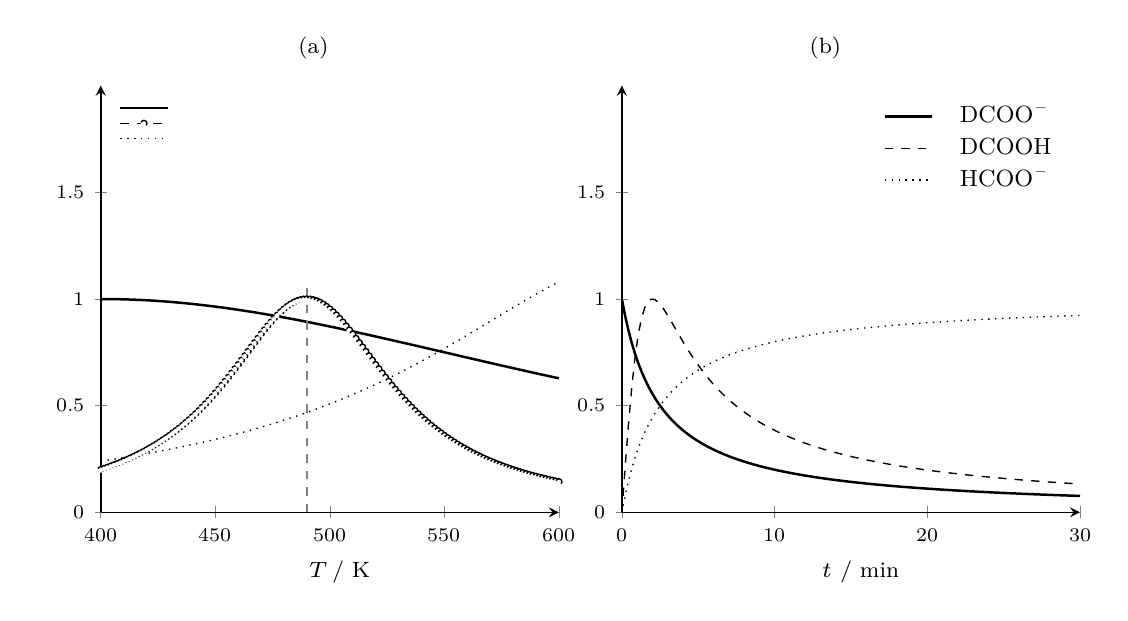
\begin{tikzpicture}
\tikzset{declare function={%
  % 参数名只用单字母，且避开 LaTeX 重音命令 \x、\u（用 \p）。
  % 函数体里的乘法一律加括号，避免 pgfmath 解析歧义。
  ads(\p)=1/(1+((\p-400)/260)*((\p-400)/260));%
  mid(\p)=1/(1+((\p-490)/45)*((\p-490)/45));%
  prd(\p)=1.2/(1+((\p-640)/120)*((\p-640)/120));%
  dcoo(\p)=1/(1+(\p/2.5));%
  hcoo(\p)=1-1/(1+(\p/2.5));%
  gdcoo(\p)=1*(\p/(1+(\p/2)*(\p/2)));}}
\begin{groupplot}[
  group style={group size=2 by 1, horizontal sep=8mm,
               ylabels at=edge left, xlabels at=edge bottom},
  % 尺寸说明：pgfplots 的 width/height 默认**含轴标签与刻度文字**（不是坐标轴盒），
  % 故 54 mm×5.2 cm 实测只得到 37.4 mm×35.4 mm 的轴盒、整图约 96 mm。
  % 这里按 74 mm×7.0 cm 反算，使两列总宽 ≈2×61+8 = 130 mm，贴近单栏图规范
  % 的 \onecolwidth（≈132 mm）而远小于版心 165 mm。
  % 两幅都把 ymax 提到 2.0，是为了给顶左/顶右的图例留出净空——图例按
  % (0.02,0.98)/(0.97,0.98) 锚定在轴顶，其像素高度固定（约 11.5 mm），
  % 提高 ymax 只把曲线整体压低，不移动图例。实测（对产出 PDF 的矢量几何核算）：
  % ymax=1.6 时「候选中间体」峰值与白心圆点标记会擦到图例第三行下沿
  % （重叠 0.2—0.6 mm），ymax=1.4 时面板 (b) 的 HCOO 曲线穿过图例第三行
  % （重叠约 1.3 mm）；改为 2.0 后两处净空均 ≥3 mm。放大尺寸后净空进一步增大。
  width=74mm, height=7.0cm, samples=141,
  axis lines=left,
  x tick label style={/pgf/number format/1000 sep={},
                      font={\fontsize{7}{8.5}\selectfont}},
  y tick label style={font={\fontsize{7}{8.5}\selectfont}},
  xlabel style={font={\fontsize{8}{9.5}\selectfont}},
  ylabel style={font={\fontsize{8}{9.5}\selectfont}},
  ]
  % 公共 domain 会被子面板继承（会报 Dimension too large），故逐面板显式给
  % domain 与 xmin/xmax：面板 (a) 是 400—600 K，面板 (b) 是 0—30 min。
  % 说明：两幅都把 ymax 提到 2.0，是为了给顶左/顶右的图例留出净空——
  % 图例按 (0.02,0.98)/(0.97,0.98) 锚定在轴顶，其像素高度固定（约 11.5 mm），
  % 提高 ymax 只把曲线整体压低，不移动图例。实测（对产出 PDF 的矢量几何核算）：
  % ymax=1.6 时「候选中间体」峰值与白心圆点标记会擦到图例第三行下沿
  % （重叠 0.2—0.6 mm），ymax=1.4 时面板 (b) 的 HCOO 曲线穿过图例第三行
  % （重叠约 1.3 mm）；改为 2.0 后两处净空均 ≥3 mm。
  \nextgroupplot[domain=400:600, xmin=400, xmax=600, ymin=0, ymax=2.0,
                 xtick={400,450,500,550,600}, ytick={0,0.5,1.0,1.5},
                 xlabel={温度 $T$ / K},
                 ylabel={相对强度（模型）},
                 title={(a) 升温序列},
                 title style={font={\fontsize{8}{9.5}\selectfont}},
                 legend style={font={\fontsize{7}{8.5}\selectfont}, draw=none,
                               fill=none, cells={anchor=west},
                               at={(0.02,0.98)}, anchor=north west}]
    % 注意：declare function 的形参只用安全单字母（\p），但 \addplot 的表达式里
    % 必须把绘图自变量 x 作为实参传进去（写成 ads(\p) 会报 Undefined control sequence）。
    \addplot[mainline, black] {ads(x)};
    \addlegendentry{甲酸盐（库）}
    \addplot[thinline, black, dashed, mark=*, mark size=1.1pt,
             mark options={fill=white}] {mid(x)};
    \addlegendentry{候选中间体}
    \addplot[thinline, black, dotted] {prd(x)};
    \addlegendentry{产物速率}
    \draw[gray, dashed] (axis cs:490,0) -- (axis cs:490,1.05);
    \node[anchor=west, font={\fontsize{7}{8.5}\selectfont}]
      at (axis cs:494,0.12) {极大};
  \nextgroupplot[domain=0:30, xmin=0, xmax=30, ymin=0, ymax=2.0,
                 xtick={0,10,20,30}, ytick={0,0.5,1.0,1.5},
                 xlabel={时间 $t$ / min},
                 title={(b) 同位素置换序列},
                 title style={font={\fontsize{8}{9.5}\selectfont}},
                 legend style={font={\fontsize{7}{8.5}\selectfont}, draw=none,
                               fill=none, cells={anchor=west},
                               at={(0.97,0.98)}, anchor=north east}]
    \addplot[mainline, black] {dcoo(x)};
    \addlegendentry{表面 \ce{DCOO-}}
    \addplot[thinline, black, dashed] {gdcoo(x)};
    \addlegendentry{气相 \ce{DCOOH}}
    \addplot[thinline, black, dotted] {hcoo(x)};
    \addlegendentry{表面 \ce{HCOO-}}
\end{groupplot}
\end{tikzpicture}
\caption{把两条判据画成序列：吸附态的「库」与真正中间体在升温过程中的消长
（a），以及同位素置换后表面物种与气相组成的走向（b）}
\label{fig:ch07c-transient}
\modelmark\ 两幅均为模型计算，不是实验谱；曲线用有界洛伦兹型与
$1/(1+t)$ 型函数构造，只用于说明判据的形状特征，不代表任何体系的实际数值。
读者应看的是两处\textbf{形状差异}：(a) 中候选中间体（虚线加圆点）在
$490$\,K 处出现极大，其后被消耗，而产物速率（点线）在更高温度才接近饱和
——「先有极大、后有产物」正是判据一要求的消长关系；储量大的甲酸盐（实线）
则单调缓降，与产物速率没有这种对应。(b) 中置换开始后表面 \ce{DCOO-}（实线）
迅速衰减，同时\emph{气相} \ce{DCOOH}（虚线）出现一个峰、再随吹扫下降，
而表面 \ce{HCOO-}（点线）上升——D 是以反应物分子的形式离开表面回到气相，
而不是以含 D 的产物出现的，这正是判据三、四要区分的情形。局限：(a) 的横轴
是模型温度标尺，(b) 的时间轴按「置换后连续采谱」设定，两者的绝对刻度都不能
用于定量；真实体系中还须叠加气相带扣除与覆盖度校正。
\figsrc{判据（分解速率与总包速率的两个数量级之差、\ce{ZnO} 上两者相等、
DCOOD 的同位素位移与置换后 \ce{DCOO-} 回到气相）据原书 §7.6.1，
书内 p.499—501 / PDF p.518—520；曲线形式为本节模型设定。}
\end{figure}

\begin{measure}
\textbf{反应条件下的原位测量。}以本书给出的原位吸附／反应流程为例
（原书图 7-93）：\ce{H2}、\ce{He}、合成气与乙醇分别经质量流量计计量后进入
原位高温高压漫反射红外原位池，池后接背压调节器再排气，从而在加压条件下
保持反应气氛与压力可控\src{S1 §7.6.3，书内 p.503—504 / PDF p.522—523}。
这套流程的三个要点与判据直接相关：①进料可切换（才能做置换实验）；
②压力与流量可独立设定（才能在同一覆盖度下比分解速率）；③池后可在线的
质谱／色谱取样（才能把表面物种与产物速率放在同一时间轴上）。
\begin{itemize}
  \item \textbf{组合实验}：\ce{Cu/ZnO/Al2O3}（Cu $60\%$、ZnO $30\%$、
        \ce{Al2O3} $10\%$，质量分数）上，只有 \ce{CO2} 与 \ce{H2} 共吸附
        才能形成甲酸盐中间物；多晶 Cu 上甲酸盐分解可给出甲醇，而 \ce{ZnO}
        上甲酸盐分解只给出 \ce{CO2}、CO 与 \ce{H2}
        \src{S1 §7.6.2，书内 p.501—502 / PDF p.520—521}。
  \item \textbf{TPSR 与在线分析}：把 DRIFTS 与 TPSR 结合，同时用在线质谱与
        色谱分析，是阐明吸附物种性质与反应机理最有力的组合。源文强调，
        \ce{Cu-ZnO-Al2O3}（ICI）上甲醇的脱出温度比纯 \ce{ZnO} 上低，
        这才是「甲酸铜盐是甲醇合成关键中间物」的支撑证据（而不是某个带位）
        \src{S1 §7.6.2，书内 p.502—503 / PDF p.521—522}。
  \item \textbf{时间分辨与瞬态}：步进扫描时间分辨红外可把时间窗压到微秒；
        快速扫描 FTIR 用于跟踪 $300$\,ms 光脉冲之后的衰减；水相光催化体系
        用金刚石单晶与 \ce{ZnSe} 晶体组成的全反射池
        \src{S1 §7.6.4，书内 p.510—512 / PDF p.529—531}。
  \item \textbf{电化学条件}：薄层电解池 + 电位差谱 + 锁相检测；参比电位必须
        固定并写明（例如以某一电位的谱作为参考谱），否则「电位依赖」的结论
        无法复现\src{S1 §7.6.4 之后，书内 p.515 / PDF p.534}。
\end{itemize}
\end{measure}

\subsubsection{判例一：甲酸在 \ce{Al2O3} 与 \ce{ZnO} 上的分解}

甲酸分解是催化选择脱氢与脱水的典型反应，也是「吸附态不等于中间体」这一
结论最干净的判例\src{S1 §7.6.1，书内 p.498—501 / PDF p.517—520}。

\begin{obs}
（只列谱学与动力学事实）
\begin{itemize}
  \item[(a)] $100$\,\degC 下甲酸吸附在 \ce{Al2O3} 上，在 $1000$—
        $4000\;\mathrm{cm^{-1}}$ 范围内出现 $2915\;\mathrm{cm^{-1}}$
        （C--H 伸缩）与 $1625\;\mathrm{cm^{-1}}$（O--C--O 反对称伸缩）等带，
        另有 $\delta(\mathrm{C{-}H})$ 与 O--C--O 对称伸缩带；表面存在
        \ce{HCOO-} 吸附态。
  \item[(b)] 改用 \ce{DCOOD} 吸附：O--H 带由 $3580\;\mathrm{cm^{-1}}$ 移到
        约 $2650\;\mathrm{cm^{-1}}$，C--H 带移到约 $2200\;\mathrm{cm^{-1}}$，
        $\delta(\mathrm{C{-}H})$ 移到约 $1029\;\mathrm{cm^{-1}}$；
        谱上没有发现 CO、\ce{CO2} 或分子态甲酸的吸附带。
  \item[(c)] 在反应温度、真空下，\ce{Al2O3} 上 \ce{HCOO-} 吸附态的分解速率
        比同温同覆盖度下甲酸蒸气的分解速率\emph{小两个数量级}。
  \item[(d)] 把 \ce{DCOOD} 分解做到定态后，用 \ce{HCOOH} 迅速置换气相并继续
        反应：表面 \ce{DCOO-} 的带消失，但它以甲酸蒸气（\ce{DCOOH}）的形式
        出现在气相；表面 O--D 迅速被 O--H 置换。
  \item[(e)] 质子交换：\ce{Al2O3} 本身的表面质子可与 \ce{H2O} 中的质子交换；
        甲酸本身的质子在 $180$\,\degC 以下不能交换；而甲酸在 \ce{Al2O3} 上
        解离吸附形成的质子，既可与 \ce{H2O} 中的质子交换，也可与甲酸中的
        质子交换。
  \item[(f)] 用盐酸或乙酸预处理 \ce{Al2O3}，表面甲酸离子浓度降到约十分之一，
        甲酸分解速率不变；吸附的乙酸没有明显分解，也没有观察到乙酸离子与
        甲酸离子之间有明显交换。
  \item[(g)] 由密闭系统的 C、H、O 物料平衡与反应气中反应物、产物分压，得到
        定态总包速率方程，形式为对甲酸一级、被水抑制
        （源文形式：$r=k(\ce{HCOOH})/[1+b(\ce{H2O})]$）。
  \item[(h)] \ce{ZnO} 表面也存在 \ce{HCOO-}，但其行为与 \ce{Al2O3} 不同：
        甲酸在 \ce{ZnO} 上分解的控速步骤是 \ce{HCOO-} 分解，且 \ce{HCOO-}
        的分解速率等于甲酸分解的总包速率。
\end{itemize}
\end{obs}

\begin{infer}
\begin{itemize}
  \item 由 (b) 得：三个带的位移比都落在 $1.3$—$1.4$ 之间（约
        $3580/2650\approx1.35$、$2915/2200\approx1.33$），符合
        式~\eqref{eq:ch07c-isotope} 对含 \ce{X-H} 振动的预言，因此
        $3580\;\mathrm{cm^{-1}}$ 归 O--H、$2915\;\mathrm{cm^{-1}}$ 归 C--H
        的归属被\emph{独立}验证；而 (b) 中不出现分子态甲酸与 CO／\ce{CO2}
        的吸附带，说明该温度下表面物种以甲酸盐与羟基为主。
  \item 由 (c) 与判据二得：\ce{Al2O3} 上的 \ce{HCOO-} 是旁观者，不是中间体。
        这条结论之所以有力，是因为它把「量」与「速率」分开了：\ce{HCOO-}
        的确存在、量也不小，但它的分解慢两个数量级，无法承担总包速率。
  \item 由 (d) 得：\ce{DCOO-} 消失的主要通道是\textbf{被气相置换回甲酸分子}，
        而不是分解成产物——即它是一个可逆吸附的「库」。这一条同时给出了
        判据三的强用法：只看表面物种消失会误判，必须同时看气相组成。
  \item 由 (f) 得：把候选物种的量减少一个数量级而活性不变，直接否掉了
        「甲酸离子是中间体」这一长期默认结论。这是判据四最干脆的一次应用。
  \item 由 (e) 与 (f) 合起来给出一条正向结论：真正参与反应的是甲酸解离吸附
        形成的\textbf{质子}，其作用类似于液相催化中 \ce{H2SO4} 提供质子的
        作用；甲酸根不参与。
  \item 由 (g) 得：速率方程的形式与上面的机理自洽——对甲酸一级（质子的
        来源）、被水抑制（水与甲酸竞争表面位或参与质子转移）。
  \item 由 (h) 得：同一物种在 \ce{ZnO} 上\textbf{是}中间体。因此
        「\ce{HCOO-} 是不是中间体」没有统一答案，必须逐体系按判据二判定。
  \item \textbf{限度}：源文明确指出，这并没有排除在其他反应条件下经甲酸离子
        分解的可能性，只是那条路径需要较高的活化能，要在较高温度下才可能
        发生。判据给出的结论都有条件范围。
\end{itemize}
\end{infer}

\subsubsection{判例二：\ce{Cu/ZnO} 上甲醇合成与乙醇助剂}

\begin{dataflow}
这个体系的信息量最大，也最能说明「多手段合成一条证据链」的做法。链条是：
\textbf{DRIFTS 给物种}（有哪些表面物种、含量随条件怎么变）→
\textbf{TPSR + 在线质谱给温度对应}（哪个物种分解时出现哪个产物）→
\textbf{反应物组合实验给来源}（该物种由哪些反应物生成）→
\textbf{活性数据给结论}（改条件后产物生成速率怎么变）。任何单独一环都不足以
判定中间体：源文列出的三个长期未决问题（C 源是 CO 还是 \ce{CO2}、活性中心
在金属 Cu 表面还是 \ce{ZnO} 表面、Cu 与 \ce{ZnO} 之间是否有协同作用），
正是单靠一种手段回答不了的\src{S1 §7.6.2，书内 p.501 / PDF p.520}。
\end{dataflow}

\textbf{物种与来源。}\ce{Cu/ZnO/Al2O3} 催化剂中 Cu 含量高且高度分散，
透射法不可能用于研究，文献中已发表的甲醇合成红外结果都是在 Cu 含量低于
$15\%$ 时取得的\src{S1 §7.6.2，书内 p.501 / PDF p.520}。改用漫反射后，
本书作者报告：$9\%$ \ce{CO2} $+$ $91\%$ \ce{H2} 于 $200$\,\degC 在 ICI
催化剂上共吸附的 DRIFT 谱与甲醇吸附谱很相似；谱上出现吸附在 Cu 上的表面
甲酸盐的 O--C--O 反对称伸缩带与对称伸缩带，其中对称伸缩带在
$1360\;\mathrm{cm^{-1}}$ 附近；\ce{ZnAl2O4} 上甲酸盐的吸收带、以及单碳酸盐
的吸收带（通常在 \ce{Al2O3} 表面上）位置各不相同\src{S1 §7.6.2，书内
p.502 / PDF p.521}。TPSR 结果给的是判据二与判据四的信息：表面甲酸盐释出时，
气相中出现甲醇以及 \ce{CO2}、\ce{H2}；且 \ce{Cu-ZnO-Al2O3}（ICI）上甲醇的
脱出温度比纯 \ce{ZnO} 上低。由于铜甲酸盐只由 \ce{CO2} 与 \ce{H2} 共吸附
形成，而多晶 Cu 上甲酸盐分解可以给出甲醇、\ce{ZnO} 上甲酸盐分解只给出
\ce{CO2}、CO 与 \ce{H2}，结论是：\textbf{甲酸铜盐是甲醇合成的关键中间物，
而 \ce{ZnO} 上的甲酸盐只是水煤气变换反应的中间物}；\ce{ZnO} 的贡献主要
是通过相互作用调变 Cu 的电子性质（氧阴离子从 \ce{ZnO} 溢流到金属铜上，
增加金属功函数），从而使甲酸盐加氢到甲氧基、再到甲醇更容易进行。

\textbf{乙醇助剂：把中间物换成酯。}工业合成甲醇需高温高压，单程 CO 转化率
只有 $20\%$ 左右；当反应系统中加入乙醇时，反应可在低温低压进行，单程 CO
转化率可达 $50\%$—$80\%$，说明反应路径本身被改变了\src{S1 §7.6.3，
书内 p.503 / PDF p.522}。原位 DRIFTS 给出的表面物种序列是：

\begin{itemize}
  \item 合成气在 \ce{Cu/ZnO} 上先形成甲酸盐物种（\ce{H-COO-Zn} 与
        \ce{H-COO-Cu} 两类）；甲酸盐在 $523$\,K 以下没有被明显加氢，而在
        $523$—$573$\,K 明显分解与加氢，气相中出现甲醇
        \src{S1 §7.6.3，书内 p.505 / PDF p.524}。
  \item 引入乙醇后，谱上出现\textbf{乙氧基}、\textbf{乙酸盐}与
        \textbf{碳酸盐}三类新物种的带；其中碳酸盐与气相乙醇反应生成
        \textbf{甲酸乙酯}物种\src{S1 §7.6.3，书内 p.505—506 / PDF
        p.524—525}。
  \item 甲酸乙酯在石英砂上没有明显的加氢，而在 \ce{Cu/ZnO} 催化剂上被加氢
        成甲醇和乙醇；进一步研究表明，完成加氢的是催化剂中 Cu 上解离吸附的
        氢\src{S1 §7.6.3，书内 p.505 / PDF p.524}。
  \item 由此提出的机理是：合成气（CO、\ce{CO2}、\ce{H2}）在 \ce{Cu/ZnO} 上
        形成甲酸盐物种，与气相或物理吸附的乙醇反应生成甲酸乙酯中间物种，
        最后被 Cu 上的氢还原成甲醇和乙醇（原书图 7-101）。甲酸乙酯是低温
        合成反应的关键中间物，它\emph{改变了经甲氧基的反应机理}
        \src{S1 §7.6.3，书内 p.507—508 / PDF p.526—527}。
\end{itemize}

上述各物种的谱带归属汇总于 \tabref{tab:ch07c-formate}。

\begin{table}[htbp]
\centering
\caption{\ce{Cu/ZnO} 表面相关物种的红外谱带归属\src{据 S1 表 7-19、表 7-20
与图 7-95～图 7-100，书内 p.505—511 / PDF p.524—530 整理。}}
\label{tab:ch07c-formate}
\begin{tabularx}{\onecolwidth}{@{}>{\raggedright\arraybackslash}p{27mm}
  >{\raggedright\arraybackslash}p{33mm} X@{}}
\toprule
表面物种 & 谱带 $/\mathrm{cm^{-1}}$ & 归属与判读要点 \\
\midrule
甲酸盐（Zn 上，\ce{b-HCOO-Zn}） & 2966（sh）、2873；1590（sh）、1572；1370、1362 &
$\nu(\mathrm{C{-}H})$、$\nu_{\mathrm{as}}(\mathrm{OCO})$、$\nu_{\mathrm{s}}(\mathrm{OCO})$
分别对应三组带；三组在表 7-19 中同归 \ce{b-HCOO-Zn} \\
甲酸盐（Cu 上，\ce{b-HCOO-Cu}） & 2925、2849；1542（sh）；1351 &
$\nu(\mathrm{C{-}H})$、$\nu_{\mathrm{as}}(\mathrm{OCO})$、$\nu_{\mathrm{s}}(\mathrm{OCO})$；
铜甲酸盐是甲醇合成的关键中间物（由 \ce{CO2}$+$\ce{H2} 共吸附生成，
TPSR 上甲醇脱出温度与它对应） \\
甲氧基（\ce{CH3O-Zn}） & 2935、2818；1049 &
$\nu(\mathrm{C{-}H})$ 与 $\nu(\mathrm{C{-}O})$；合成气吸附后 ZnO 上即出现
甲氧基，是甲醇合成的另一条路径 \\
表面水（\ce{H2O-Cu}） & 1601 &
$\delta(\mathrm{OH})$；残余表面水的弯曲振动，判读时须与甲酸盐的
$\nu_{\mathrm{as}}(\mathrm{OCO})$ 带区分 \\
乙氧基（乙醇引入后） & 2961、2925、2889、2861；1440、1380；1101、1052 &
$\nu(\mathrm{C{-}H})$、$\delta(\mathrm{CH})$、$\nu(\mathrm{C{-}O})$；
出现乙氧基说明乙醇已解离吸附在表面 \\
羧酸基（乙酸盐，乙醇引入后） & 2933；1562、1451；1049、1023 &
$\nu(\mathrm{C{-}H})$、$\nu(\mathrm{OCO})$ 与 $\rho(\ce{CH3})$；
乙酸物种的出现是乙醇被氧化的旁路证据 \\
碳酸盐（乙醇引入后） & 1551、1534、1428、1345 &
$\nu(\mathrm{COOO})$ 伸缩分裂；碳酸盐可与气相乙醇反应生成甲酸乙酯，
是助剂路径上的关键一环 \\
\bottomrule
\end{tabularx}
\end{table}

\tocheck{未对照原页面图像：原书表 7-19、表 7-20 的列结构在 OCR 中被打乱
（乙氧基／羧酸基／碳酸盐三列的带位互相穿插），上表的带位分组是按源文本可辨
数值与「同一物种的带应成组出现」这一约束重建的；$1360$（甲酸盐对称伸缩）
与源表 $1370/1362$ 几个相近数值的归属、以及 $1551/1534$、$1428/1345$
两组碳酸盐带的配对方式，均未与原页面图像核对。}

\begin{pitfall}
\textbf{把吸附态当中间体。}这是本领域最经典的误判：\ce{Al2O3} 上
\ce{HCOO-} 长期被当成甲酸分解的中间物，直到用判据二测出它的分解速率比总包
速率小两个数量级才被否掉。判据一（序列上的消长）单独用也不够：储量大的物种
在升温过程中常常也「先升后降」（因为总覆盖度下降），必须与产物速率的
\emph{量级}比较。

\textbf{只凭位置归属，不做对照实验。}$1360\;\mathrm{cm^{-1}}$ 这样的带位
可以同时属于甲酸盐、乙酸盐甚至碳酸盐的 O--C--O 伸缩；只有把「共吸附组合
实验」（只有 \ce{CO2}$+$\ce{H2} 才生成）、「温度对应」（TPSR 上产物脱出
温度）与「对照样品」（石英砂上甲酸乙酯不加氢，\ce{Cu/ZnO} 上加氢）放在
一起，归属才成立。

\textbf{忽略气相物种的贡献。}反应条件下的谱图里，气相反应物与产物都有红外
吸收：气相 CO（$2143\;\mathrm{cm^{-1}}$）、气相 \ce{CO2}（$2349\;
\mathrm{cm^{-1}}$）、气相甲酸与乙醇在 $1000$—$3000\;\mathrm{cm^{-1}}$ 有
多条带。若不扣除气相贡献（用背景谱、吹扫对比或差谱），表面物种的带强度与
位置都会被污染；甲酸乙酯这类「气相或物理吸附」的物种更要在图题里写清是
气相带还是表面带。

\textbf{忽略原位池窗口与样品自吸收造成的强度失真。}池窗材料的截止波数、
样品稀释度、装样厚度以及（漫反射下）散射系数的变化，都会改变基线。跨样品
比强度是这一体系上最容易出错的一步；同一体系内部不同温度的强度比较，也要
扣除总覆盖度的变化。

\textbf{把「光照依赖」直接当成光催化中间体的证据。}光照会同时改变温度、
吸附平衡与表面电荷，故光催化体系里必须给出电位或时间依赖，并配合同位素
实验（如 \ce{H2^{18}O} 交换）才能把中间物种与光生载流子过程连起来。
\end{pitfall}

\subsubsection{光催化水氧化：把判据用到光生载流子上}

半导体光催化中，光催化剂先吸收入射光子产生光生电子与空穴，随后经历扩散、
捕获、复合与表面氧化还原反应；水氧化产氧是四空穴转移过程，往往涉及多种
中间物种，特别是不同状态的氧物种，因此原位红外（以及时间分辨红外）在
认识光催化机理中起的作用很重\src{S1 §7.6.4，书内 p.508—510 / PDF
p.527—529}。三条有代表性的证据链：

\begin{itemize}
  \item \textbf{金红石 \ce{TiO2} 上的两个产氧中间物。}用金刚石单晶与
        \ce{ZnSe} 晶体组成的全反射红外池原位研究光激发下金红石 \ce{TiO2}
        纳米颗粒；在 \ce{Fe^{3+}} 作电子牺牲试剂的条件下，光激发时表面出现
        位于 $838$ 与 $812\;\mathrm{cm^{-1}}$ 的两个中间物带，同位素实验将
        它们分别归属为 \ce{TiOOH} 与 \ce{TiOO-Ti}；由此提出 \ce{H2O} 分子
        亲核进攻表面晶格氧空穴生成上述中间物的反应路径
        \src{S1 §7.6.4，书内 p.510 / PDF p.529}。
  \item \textbf{\ce{Co3O4} 上的过氧双核物种。}用快速扫描 FTIR 研究
        \ce{Co3O4} 纳米粒子在 $\mathrm{Ru(bpy)_3^{2+}}$ 光敏剂敏化条件下的
        放氧动力学：$300$\,ms 脉冲光激发后，存在大量未放出的
        $1013\;\mathrm{cm^{-1}}$ 氧中间物种；结合同位素实验与动力学分析，
        归属为三空穴氧化生成的过氧双核物种，并认为是放氧的关键中间物种
        \src{S1 §7.6.4，书内 p.511 / PDF p.530}。
  \item \textbf{直接跟踪光生电子。}光生电子吸收近红外和中红外光，而光生空穴
        在该波段基本没有吸收，不会干扰电子信号，因此时间分辨红外成为研究
        光生电子动力学最有效的技术之一。用步进扫描时间分辨红外研究
        \ce{TiO2}，可观察到中红外范围内的特征宽吸收，其吸光度随波数减小而
        逐渐增加，被归属为浅束缚能级与导带电子；这些电子的衰减在微秒到毫秒
        量级。甲醇存在时，Pt 负载 \ce{TiO2} 上光生电子在微秒量级基本不衰减，
        直到毫秒到秒才明显衰减，增加气相甲醇或水汽可明显促进这一衰减；结合
        光催化重整甲醇制氢的活性结果，提出分子态吸附的水与甲醇促进了质子
        转移，从而促进 Pt 上的产氢反应
        \src{S1 §7.6.4，书内 p.512—513 / PDF p.531—532}。
\end{itemize}

\tocheck{未对照原页面图像：金红石 \ce{TiO2} 上两个中间物带位的文字在 OCR 中
可辨为 838 与 $812\;\mathrm{cm^{-1}}$，但配图图注（图 7-102）中的第二处带位
与归属箭头无法辨读；时间分辨一段中样品的标号（源文作「P?25TiO2」）不能确定
是 Pt/TiO2 还是另一种 Pt 负载量标号，本分片按「Pt 负载 TiO2」表述。}

\subsubsection{电化学与光电催化原位红外：薄层、差谱与毒性中间体}

\emph{（本小节标题及其前一段文字所在的页面在源文本中缺损，标题为按内容拟定。）}
\tocheck{未对照原页面图像：书内 p.514（PDF p.533）的 OCR 层为空，该页上的
小节标题与部分正文缺失；本小节标题「电化学与光电催化原位红外」是按源文
内容（固液界面红外、薄层电解池、电催化机理）拟定的，未与原页面核对。}

固液界面的红外研究要克服三个障碍：①溶剂分子（通常为水）对红外能量的大量
吸收；②固体电催化剂表面反射红外光导致部分能量损失；③表面吸附分子量少，
满单层情况下吸附量仅在 $10^{-9}$\,mol\,cm$^{-2}$ 量级。这些障碍使信号非常
微弱，需用薄层电解池、电位差谱与各种微弱信号检测技术提高信噪比
\src{S1 §7.6.4 之后，书内 p.515 / PDF p.534}。常用的做法是让工作电极与
红外窗片紧密接触，形成很薄的液体薄层电解池，以尽量减少红外光被溶剂吸收的
量；液层厚度是这套方法的关键参数（源文引用的研究表明，只有当液层厚度小到
一定程度时才能得到较高信噪比）。电位差谱则是在保持其他实验条件不变的情况下
仅改变电极电位，再做差减归一化；锁相检测、偏振调整等技术也常用于微弱信号
检测。\tocheck{未对照原页面图像：液层厚度上限的数值在 OCR 中作「130」后接
一个损坏字符（可能为 µm），本分片未写入具体上限，只保留「需小到足够薄」
这一条件；满单层吸附量的数量级（$10^{-9}$\,mol\,cm$^{-2}$）在 OCR 中同样
残缺，按学科常见量级补写，未与原文核对。}

判据在这里的用法与前面一致，只是「序列」的变量换成了\textbf{电位}：

\begin{itemize}
  \item \textbf{CO 作探针。}在经过电化学处理的多晶 Rh 电极上可检测到两种
        CO 孪生吸附态：用较快的电位扫描速度（$1.5$\,V/s）在 $2.4$\,V 电位
        区间处理电极，可在表面形成一层 Rh 原子簇氧化物膜，使吸附 CO 给出一对
        宽的 IR 吸收带；当表面金属氧化物被还原后，CO 仍以孪生态吸附在电极
        表面，但吸收带红移到 $2012$ 与 $2032\;\mathrm{cm^{-1}}$，半峰宽减小
        \src{S1 §7.6.4 之后，书内 p.516 / PDF p.535}。
  \item \textbf{毒性中间体与结构敏感性。}甲醇的电催化氧化遵循双途径机理
        （活性中间体途径与经毒性中间体的途径）。电化学原位红外在 Pt 单晶
        电极上区分出两类毒性中间体：位于 $2050\;\mathrm{cm^{-1}}$ 左右的
        线式吸附 CO，以及多重态吸附物种；毒性中间体的起始氧化电位顺序为
        Pt(111) $<$ Pt(110) $<$ Pt(100)，说明甲醇电催化氧化是表面结构敏感
        反应\src{S1 §7.6.4 之后，书内 p.517 / PDF p.536}。
  \item \textbf{助剂如何减少毒性中间体。}在 Pd/C 电极上可以观测到 CO 带，
        而硼的引入使 Pd 表面积累的 CO 发生实质性减少；这些吸附 CO 应是主要
        的毒性中间体，其减少显著改善了甲酸燃料电池的性能（原书图 7-108 以
        $1.25$\,V 的谱作参考谱）\src{S1 §7.6.4 之后，书内 p.517 / PDF
        p.536}。
  \item \textbf{光电催化水氧化。}在 \ce{Fe2O3} 光阳极上，于光电催化水氧化
        条件下观测到 $898\;\mathrm{cm^{-1}}$ 处的新红外吸收中间物种；该吸收
        对光照存在明显依赖，仅在光电催化水氧化发生时存在，被归属为高价铁氧
        中间物种 $\mathrm{Fe^{IV}{=}O}$，即水氧化第一步空穴氧化过程的中间物
        \src{S1 §7.6.4 之后，书内 p.517—518 / PDF p.536—537}。
\end{itemize}

\begin{crosscheck}
\textbf{与电化学曲线互查。}中间物种的电位依赖必须与 $J$--$V$ 曲线、
起始氧化电位、库仑量对应；若某个带只随电位移动而与电流无关，更可能是双电层
或溶剂重组效应。

\textbf{与同位素、质谱互查。}光催化与电催化体系里，\ce{H2^{18}O} 交换可以
把「含水物种」与「含晶格氧物种」分开；微分电化学质谱可以给出产物的实时
生成速率，与红外带强度同轴比较，正是判据二在电化学条件下的形式。

\textbf{与理论计算互查。}带位归属（如 \ce{TiOOH} 与 \ce{TiOO-Ti} 的区分、
$\mathrm{Fe^{IV}{=}O}$ 的指认）最终要与频率计算和反应能垒计算一致；计算不能
替代判据，但可以排除几张谱之间无法区分的候选结构。

\textbf{回到方法边界。}红外给出的是有红外活性的物种；对称性高、偶极变化小的
物种（以及被强吸收带掩盖的物种）可能\emph{测不到}。「没看到」永远不能直接
推出「不存在」，这也是本书在光催化与电催化两节反复强调的边界。
\end{crosscheck}

\srcnote{本分片来源：S1（上册）§7.5—§7.6，以及 §7.6 之后的电化学与光电催化
原位红外部分，书内 p.489—518 / PDF p.508—537。其中书内 p.514（PDF p.533）的
OCR 层缺损，该处小节标题与部分正文缺失，已在正文用 \tocheck{} 标注。
原书参考文献与作者简介见书内 p.518—523 / PDF p.537—542，本分片不复述。
本节内所有谱带数值均取自源文本文字层，凡 OCR 残缺或互相矛盾之处均已在正文
就地标注，未对照原页面图像。}
}{}
\IfFileExists{chapters/parts/ch07-d.tex}{\input{chapters/parts/ch07-d}}{}
\IfFileExists{chapters/parts/ch07-e.tex}{\input{chapters/parts/ch07-e}}{}
}{}
\IfFileExists{chapters/ch08.tex}{% chapters/ch08.tex —— 第 8 章 核磁共振方法
% 装配层：只负责按顺序引入各分片。分片缺失时跳过，便于增量成书。
% 分片文件：chapters/parts/ch08-{a..e}.tex

\IfFileExists{chapters/parts/ch08-a.tex}{% ================================================================
%  chapters/parts/ch08-a.tex   （第 8 章 核磁共振方法，分片 a）
%  源：S2（下册）第 8 章，书内 p.525—543 / PDF p.18—35
%  覆盖：8.1 固体高分辨 NMR 技术（MAS / CP-MAS / 高功率 1H 去偶）
%        8.2 分子筛结构的 MAS NMR 研究（29Si / 27Al / 17O / 31P / 47,49Ti）
%  未覆盖（分片 b/c）：8.3 及以后（酸性、吸附分子、原位、积炭）
%  页码说明：下册印刷页 526 未出现在 PDF 中，故书内页码跳号属正常。
% ================================================================

\chapterstart{核磁共振方法}%
{本章导读：本章回答三个问题——固体谱线为什么极宽；MAS、CP、高功率去偶各自消掉哪一项
相互作用；在什么条件下一条固体 NMR 谱才能被读成结构结论。全章沿「固体高分辨技术
（8.1）$\rightarrow$ 分子筛骨架核（8.2）$\rightarrow$ 表面酸性 $\rightarrow$
吸附分子与原位 $\rightarrow$ 积炭」展开，把每一个谱学量都落到一个可检验的结构
判断上。本分片覆盖 8.1 与 8.2，其中 8.1 是后文全部案例共用的方法与条件基础。}
\label{ch:08}

\subsection{固体高分辨核磁共振技术}

\begin{probout}
固体 MAS NMR 测的是\textbf{原子核局域的电子与几何环境}：化学位移给出配位状态与键合
环境，四极耦合参数给出配位对称性，偶极耦合给出核间距与空间连接，弛豫时间给出运动性。
与 XRD 给出长程有序的晶体结构不同，它给出\textbf{所研究核的局部结构和配位信息}，因此对
短程有序、甚至非晶态的催化材料同样有效；二者结合才能得到较完整的结构图像。
\src{S2 §8，书内 p.527 / PDF p.19}
\end{probout}

固体 NMR 的全部困难可以压缩成一条因果链：

\begin{center}
\fontsize{9}{13}\selectfont
固体中分子不能像液体那样快速各向同性翻滚 $\rightarrow$ 各种内部相互作用不被运动平均
$\rightarrow$ \textbf{谱线极宽}（固体线宽常大于 \qty{100}{kHz}，而液体 \ce{H2O} 的线宽
小于 \qty{1}{Hz}）$\rightarrow$ 分辨率与灵敏度同时塌陷 $\rightarrow$ 必须针对\textbf{每一种}
相互作用设计专门的抵消手段 $\rightarrow$ 才得到可归属、可定量的窄线谱
\end{center}

这条链的关键在于：窄化手段不是通用的「去噪」，\textbf{每一种手段只抵消链上的一到两项}。
把来源与对策一一对应起来，才能判断一张谱在什么条件下可信（表~\ref{tab:narrow-map}）。

\begin{table}[htbp]
\centering
\caption{固体谱线增宽来源与对应窄化手段的一一对应。读者应看第三列：任何一张谱都要说清
它用了哪几种手段，未消除的那一项就是该谱的固有局限。\src{据 S2 §8.1，书内 p.527—531 / PDF p.19—23 归纳。}}
\label{tab:narrow-map}
{\srcsize
\begin{tabularx}{\columnwidth}{@{}lXX@{}}
\toprule
增宽来源 & 表现与量级 & 对应窄化手段 \\
\midrule
同核/异核偶极--偶极 & 与 $\gamma_1\gamma_2/r^3$ 成正比；$^{1}$H、$^{19}$F 同核偶极可达 \qty{100}{kHz} & MAS（空间部分）+ 高功率异核去偶、同核多脉冲（自旋部分） \\
化学位移各向异性（CSA） & 粉末线型宽达数十至数百 ppm & MAS；静态谱反而用来直接读张量主值 \\
四极相互作用（$I>1/2$） & 一阶极大；中心跃迁只余二阶，二阶增宽 $\propto 1/B_0$ & 一阶由 MAS 消除；二阶需高场、MQ MAS 或 DOR/DAS \\
标量（$J$）耦合 & 固体中通常较小 & 去偶、脉冲序列选择 \\
弛豫过快（$T_2$ 短） & 线宽 $\approx 1/(\pi T_2)$ & 降低温度、改善样品均匀性；无法靠脉冲消除 \\
\bottomrule
\end{tabularx}}
\end{table}
\emph{核对说明}：已对照原页面图像（书内 p.531 / PDF p.23）。该页（§8.1.4 高功率
$^{1}$H 去偶）印：同核偶极作用很大时，如 $^{1}$H 和 $^{19}$F 核的同核偶极作用（HD）为
100 kHz，只有满足快速魔角旋转条件，即 $\omega R \gg |HD|_{\max}$，
才可能消除同核偶极作用；一般探头的魔角旋转速度难以达到 111 kHz 超高速 MAS 探头的转速，所以 MAS
技术通常无法消除同核偶极作用；异核去偶（CW 与 TPPM）消除的是 $^{1}$H 对 $^{13}$C
等异核的偶合。本表「同核偶极增宽」一行据该页。化学位移各向异性、四极相互作用、标量 $J$ 耦合、
弛豫过快四行的来源页为 §8.1.3（书内 p.527--531 / PDF p.19--23），
\textbf{尚未逐页核对}。

\begin{principle}
\textbf{增宽的五类来源。}（1）\textbf{核的偶极--偶极相互作用}：同核与异核皆有，大小取决于
核磁矩与核间距；固体中核运动受限，偶极作用比流体样品强，$^{1}$H 等磁矩大的丰核尤其强，
是固体谱增宽的主要因素之一。（2）\textbf{化学位移各向异性}：分子对外磁场取向不同时核外
磁屏蔽与共振频率不同；溶液中各向同性快速运动把它平均成单一值，固体中则表现为宽线，
球对称、轴对称与低对称分子的宽线峰形各不相同。（3）\textbf{四极相互作用}：$I>1/2$ 的核
都存在，溶液中快速翻转把它平均掉，固体中使谱线大大加宽。（4）自旋--自旋标量耦合；
（5）自旋--自旋弛豫时间过短。\textbf{自旋 $I=1/2$ 的核只有（1）（2）两类}；四极核除
（1）（2）外一般以（3）为主。\src{S2 §8.1，书内 p.527—528 / PDF p.19—20}
\end{principle}

\begin{measure}
\textbf{仪器与实验条件。}固体谱仪必须配魔角旋转（MAS）探头，并需要高射频功率
（约 \qty{1000}{W}）以获得短脉冲和宽激发带宽，而液体谱通常只需约 \qty{100}{W}。
转速决定能平均掉多强的相互作用：常见探头为几千赫至十几千赫，可消除 CSA，但只能部分
消除偶极作用；2.5 mm 转子探头可达 \qty{30}{kHz} 以上，最新商业化的 0.7 mm 转子可达
\qty{111}{kHz}。\src{S2 §8.1、§8.1.2，书内 p.528、p.530 / PDF p.20、p.22}
\end{measure}

按自旋量子数，可观测核分为三类，这决定了后面每个核种能问什么问题：$I=1/2$ 核
（$^{1}$H、$^{13}$C、$^{29}$Si、$^{15}$N、$^{31}$P、$^{129}$Xe、$^{195}$Pt 等）；
半整数四极核 $I=3/2,\,5/2,\,7/2,\,9/2$（$^{11}$B、$^{23}$Na、$^{7}$Li、$^{27}$Al、
$^{51}$V、$^{93}$Nb 等）；整数四极核 $I=1,\,3$（$^{2}$H、$^{14}$N、$^{6}$Li、$^{10}$B 等）。
\src{S2 §8.1，书内 p.528 / PDF p.20}

\subsubsection{固体 NMR 的发展过程}

整条发展线索只有一个目标：提高分辨率与灵敏度、建立核与核之间的关联。1958 年 Andrew 与
Lowe 提出魔角旋转（MAS），大大消除了化学位移各向异性与同核偶极作用；1962 年 Hartmann 与
Hahn 提出交叉极化（CP），通过极化转移增强稀核灵敏度；1968 年 Waugh 等实现 WAHUHA 四脉冲
同核去偶；1988 年 Pines 等发展双旋转（DOR）与动态变角旋转（DAS）以消除半整数四极核中心
跃迁的二阶四极作用，因需特殊探头而推广受限；1989 年 REDOR 开创异核间距测量；1994 年
DQ-MAS 建立同核间距测量；1995 年 Frydman 提出多量子魔角旋转（MQ MAS），无需特殊硬件即可
在商用谱仪上消除二阶四极作用，把四极核 NMR 推上一个台阶。本节以下只展开其中三项与分子筛
研究直接相关者。\src{S2 §8.1.1，书内 p.529 / PDF p.21}

\subsubsection{魔角旋转固体核磁共振技术（MAS NMR）}

静态粉末谱直接呈现化学位移各向异性。屏蔽张量的主值为 $\delta_{11}$、$\delta_{22}$、
$\delta_{33}$，由此定义三个可测量量：

\begin{equation}
\label{eq:csatensor}
\begin{aligned}
\delta_{\mathrm{iso}} &= \tfrac{1}{3}\left(\delta_{11}+\delta_{22}+\delta_{33}\right)\\
\Delta\delta &= \delta_{33}-\tfrac{1}{2}\left(\delta_{11}+\delta_{22}\right)\\
\eta &= \left(\delta_{22}-\delta_{11}\right)\big/\left(\delta_{33}-\delta_{\mathrm{iso}}\right)
\end{aligned}
\end{equation}

式中 $\delta_{\mathrm{iso}}$ 为各向同性化学位移，$\Delta\delta$ 为各向异性张量差，
$\eta$ 为不对称因子。\textbf{从静态谱可以直接读出张量的三个主值}；另一个等价途径是拟合
旋转边带，因为边带的包络线就是粉末线型。
（此处已对照原页面图像（书内 p.529 / PDF p.21）：原书逐字印
$\delta_{\mathrm{iso}}=\tfrac{1}{3}(\delta_{11}+\delta_{22}+\delta_{33})$、
$\Delta\delta=\delta_{33}-\tfrac{1}{2}(\delta_{11}+\delta_{22})$、
$\eta=(\delta_{22}-\delta_{11})/(\delta_{33}-\delta_{\mathrm{iso}})$，
$\eta$ 的分母确为 $\delta_{33}-\delta_{\mathrm{iso}}$，三式与上式一致。）
\src{S2 §8.1.2，书内 p.529 / PDF p.21}

使谱线窄化，除高功率 $^{1}$H 去偶外最主要的技术是\textbf{魔角旋转}：把固体样品装在转子中，
绕与外加磁场成 $54.7^\circ$ 的轴高速旋转。旋转样品的磁屏蔽常数写作

\begin{equation}
\label{eq:sigma1}
\begin{aligned}
\sigma_{\mathrm{rot}}&=\sigma_{\mathrm{iso}}
+\frac{1}{2}\left(3\cos^{2}\beta-1\right)\cdot\frac{\delta}{2}
\Bigl[\,3\cos^{2}\theta-1+\eta\sin^{2}\theta\cos 2\phi\,\Bigr]
\end{aligned}
\end{equation}

式中 $\beta$ 为\textbf{样品（转子轴）与外磁场方向 $B_0$ 的夹角}，$\sigma_{\mathrm{iso}}$ 为
各向同性磁屏蔽常数，$\delta$、$\eta$ 反映屏蔽矩阵的各向异性和非对称性，$\theta$、$\phi$
为\textbf{屏蔽环境（分子）坐标系中张量主轴相对转子轴的取向}。
两个角分工不同，不能互换：$\beta$ 由实验者通过转子取向设定，$\theta$、$\phi$ 由分子在
转子中的排列决定、随分子翻滚而变，实验上无法逐个控制。
\textbf{量纲检查}：$\sigma$、$\delta$ 同为磁屏蔽（无量纲量，以 ppm 表示），方括号内两项
皆为「各向异性/各向同性之比」的纯数，故两边量纲一致。
（此处已对照原页面图像（书内 p.529—530 / PDF p.21—22）：原书式 (8-1) 逐字印为
$\sigma_{\mathrm{rot}}=\sigma_{\mathrm{iso}}+\tfrac{1}{2}(3\cos^{2}\beta-1)\cdot
\tfrac{\delta}{2}[\,3(\cos^{2}\theta-1)+\eta\sin^{2}\theta\cos 2\phi\,]$，
即 $\delta$ 确作公因子提到方括号外、$\eta$ 项不带 $1/2$；本处照此改写为公因子形式，
仅把方括号内首项按通行写法作 $3\cos^{2}\theta-1$（原书印 $3(\cos^{2}\theta-1)$，
两者相差常数 2、并不等价；本处按标准式取之，原印法备查）。$\beta=54.7^\circ$ 时整体归零的结论不受影响。）
\src{S2 §8.1.2，书内 p.529—530 / PDF p.21—22}

\begin{principle}
\textbf{魔角条件。}式~\eqref{eq:sigma1} 的后一项是固体特有的化学位移各向异性项，其中只有
$P_2(\cos\beta)=(3\cos^{2}\beta-1)/2$ 这一个因子与转子取向有关。\textbf{令 $P_2$ 为零，
消去的才是转子轴与外场的夹角 $\beta$}（不是局部的 $\theta$）：

\begin{equation}
\label{eq:magic}
\begin{aligned}
&3\cos^{2}\beta-1=0
\;\Longrightarrow\;\cos^{2}\beta=\tfrac{1}{3}\\
&\;\Longrightarrow\;\beta=\arccos\tfrac{1}{\sqrt{3}}=54.7356^\circ
\end{aligned}
\end{equation}

此时 $\sigma_{\mathrm{rot}}=\sigma_{\mathrm{iso}}$，各向异性作用被极大程度消除。\textbf{它
为什么能消掉一阶增宽}：化学位移各向异性、偶极--偶极作用、一阶四极作用的一阶微扰角因子
都只含同一个二阶勒让德多项式 $P_2$；快速旋转下这些含时角因子的\textbf{时间平均}正比于
$P_2(\cos\beta)$。$\beta$ 取 $54.7356^\circ$ 时 $P_2$ 归零，所以\textbf{一项几何条件同时
消掉三类一阶增宽}——这正是「魔角」之名的由来。
$54.7^\circ$ 被称为魔角，样品管在魔角位置上的整体转动即魔角旋转。
\textbf{最常见的读图错误}：$\beta$ 一律\textbf{从 $B_0$（竖直方向）量起}，
不是从水平面量起。把转子轴画成与水平面成 $54.7^\circ$ 时，它与 $B_0$ 只有 $35.3^\circ$，
此时 $P_2(\cos 35.264^\circ)\approx0.5$，各向异性\textbf{只被消去一半、并未归零}，
谱线仍宽。\src{S2 §8.1.2，书内 p.530 / PDF p.22}
\end{principle}

\begin{figure}[htbp]
\centering
% 图源几何自检（可复算）：转子轴方向 = 54.736 deg，自竖直 B_0 量起；
%   端点 (34*sin54.736, 34*cos54.736) = (27.76, 19.63) mm；
%   atan2(27.76, 19.63) = 54.7360 deg  ->  (3cos^2 - 1)/2 = 0
%   若误按 TikZ 极角 (54.736:34) 画（即自水平量起），与 B_0 夹角只有 35.264 deg，
%   P_2 = +0.5，各向异性并未消去。
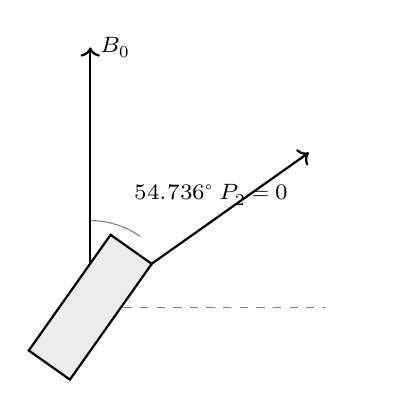
\begin{tikzpicture}[x=1mm,y=1mm]
  \draw[->,thick] (0,0) -- (0,33)
     node[right,text width=19mm,align=left,font=\fontsize{8}{9.6}\selectfont]{$B_0$：外磁场方向};
  \draw[dashed,gray] (0,0) -- (30,0);
  \draw[gray] (0,11) arc[start angle=90,end angle=54.736,radius=11];
  \node[anchor=south west,font=\fontsize{8}{9.6}\selectfont] at (4.4,11.7)
     {$54.736^\circ$（$P_2=0$）};
  \draw[->,thick] (0,0) -- (27.76,19.63)
     node[anchor=south west,font=\fontsize{8}{9.6}\selectfont] at (28.4,19.0)
     {转子轴（样品管）};
  \begin{scope}[rotate=-35.264]
    \draw[thick,fill=gray!15] (-3.2,-9) rectangle (3.2,9);
  \end{scope}
\end{tikzpicture}
\caption{魔角几何：样品管绕与 $B_0$ 成 $54.736^\circ$ 的轴旋转（$\beta$ 自\textbf{竖直的
$B_0$} 量起，与水平方向成 $35.264^\circ$）。读者应看两处——$\beta$ 由 $P_2(\cos\beta)=0$
定出，而\textbf{三类一阶增宽}（化学位移各向异性、偶极--偶极、一阶四极）\textbf{共用同一个
角因子} $P_2(\cos\beta)=\tfrac{1}{2}(3\cos^{2}\beta-1)$，故只此一个角度就把它们一起归零；
转子轴线与实心样品管长轴重合，图中画成一根轴。本图为几何示意图，
不表示真实探头尺寸与转速方向。\schemamark\figsrc{据 S2 §8.1.2，
书内 p.530 / PDF p.22 改绘。}}
\label{fig:magic-angle}
\end{figure}

\textbf{偶极耦合与核间距。}异核（或同核）两核的偶极耦合常数为

\begin{equation}
\label{eq:dipolar}
b_{12}=-\frac{\mu_0}{4\pi}\cdot\frac{\gamma_1\gamma_2\hbar}{r^{3}},
\qquad
\omega_{\mathrm{D}}(\theta)=b_{12}\cdot\frac{3\cos^{2}\theta-1}{2}
\end{equation}

式中 $\gamma_1$、$\gamma_2$ 为两核的磁旋比，$r$ 为核间距，$\theta$ 为核间矢量与外磁场的夹角。
\textbf{量纲检查}：$\mu_0$ 单位 $\mathrm{H\,m^{-1}}$，$\gamma$ 单位
$\mathrm{rad\,s^{-1}\,T^{-1}}$，$\hbar$ 单位 $\mathrm{J\,s}$，故
$\mu_0\gamma_1\gamma_2\hbar/r^{3}$ 约化后为 $\mathrm{s^{-1}}$（角频率），与 $\omega_{\mathrm{D}}$
一致；除以 $2\pi$ 即得 Hz。两条可直接使用的推论：（i）耦合按 $r^{-3}$ 衰减，核间距增加
10\% 耦合即下降约 25\%，因此偶极耦合是最近的「分子尺」；（ii）角因子 $P_2(\cos\theta)$
在 $\theta=54.736^\circ$ 为零——此处的 $\theta$ 是\textbf{核间矢量与 $B_0$} 的夹角，
与式~\eqref{eq:magic} 的转子轴夹角 $\beta$ 是两个不同的角；MAS 下核间矢量随分子一起
绕转子轴转动，其空间部分的时间平均正比于 $P_2(\cos\beta)$，故转子轴取 $\beta=54.736^\circ$
即可让偶极作用与 CSA 的时间平均\textbf{同时}归零。
\src{S2 §8.1、§8.1.2，书内 p.527、p.530 / PDF p.19、p.22}
\pedset{本处数值算例为教学补充、非原书数据：取 $^{1}$H--$^{1}$H、$r=1.0$~\AA{}，由
式~\eqref{eq:dipolar} 得 $|b|/2\pi\approx\qty{120}{kHz}$，与正文所述 $^{1}$H、$^{19}$F
同核偶极约 \qty{100}{kHz} 同量级，可用作自检。}

\begin{measure}
\textbf{转速够不够，看旋转边带。}MAS 只在「旋转比相互作用快」时把宽线收成一条中心线。
转速不足时，原本连成一片的粉末线型被切成间隔等于转速 $\nu_{\mathrm{r}}$ 的一组
\textbf{旋转边带}（spinning sidebands），中心带只是全部信号的一部分。判断规则有三条：
（i）\textbf{边带间隔等于转速}，可由间隔反读实验转速；（ii）\textbf{边带包络线就是静态
粉末线型}，因此可以用边带强度分布反过来拟合化学位移张量主值；（iii）\textbf{转速足够时
边带强度趋于零}，中心带高度不再随转速增加而上升、线宽也不再收窄。
\src{S2 §8.1.2，书内 p.529—530 / PDF p.21—22}
\end{measure}

\begin{pitfall}
把「中心带面积」当作全部信号来定量，是 MAS 谱最常见的定量错误。只要边带还有可观强度，
按中心带积分就会\textbf{系统性低估}该物种的含量；正确做法是把所有边带一并加和，或把转速
提高到边带可忽略。此外，MAS 只能平均掉偶极哈密顿量的\textbf{空间部分}：当同核偶极作用
很大时（$^{1}$H、$^{19}$F 的同核偶极可达 \qty{100}{kHz}），只有满足 $\omega_{\mathrm{R}}
\gtrsim |H_{\mathrm{D}}|_{\max}$ 的快速旋转条件才能消除它，而一般探头达不到，故
\textbf{MAS 通常并不能消除同核偶极作用}。\src{S2 §8.1.4，书内 p.531 / PDF p.23}
\end{pitfall}

\subsubsection{交叉极化/魔角旋转固体核磁共振技术（CP/MAS NMR）}
\label{sec:cp-mas}

$^{13}$C、$^{15}$N、$^{29}$Si 等稀核丰度低、磁旋比小，检测灵敏度低，且自旋--晶格弛豫
时间 $T_1$ 长，需要很长的弛豫延迟。交叉极化（cross polarization，CP）用丰核（如 $^{1}$H）
的极化去增强稀核信号，条件是两核的射频场满足 Hartmann--Hahn 匹配：

\begin{equation}
\label{eq:hh}
\gamma_{S}B_{1S}=\gamma_{I}B_{1I}
\qquad (I,\,S\ \text{均为}\ I=1/2)
\end{equation}

式中 $S$ 为稀核、$I$ 为丰核。满足匹配即实现极化由丰核向稀核转移，例如 $^{1}$H--$^{13}$C
交叉极化可使 $^{13}$C 信号增强 $\gamma_{\mathrm{H}}/\gamma_{\mathrm{C}}\approx4$ 倍。
CP 脉冲序列中两核同时自旋锁定，其有效的弛豫延迟取决于丰核（$^{1}$H）的
$T_{1\rho}$，而 $^{1}$H 的 $T_{1\rho}$ 往往比 $^{13}$C 的 $T_1$ 短得多，因此信号累加
效率大大提高，对检测季碳尤其有利。当稀核为半整数四极核时，匹配条件变为

\begin{equation}
\label{eq:hhquad}
\nu_{1A}=\left(I+\frac{1}{2}\right)\nu_{1B}
\end{equation}

式中 $A$ 代表 $I=1/2$ 核，$B$ 为四极核。$^{27}$Al 的 $I=5/2$，故静态下 $^{1}$H$\rightarrow
^{27}$Al 的 CP 要求 $\nu_{1\mathrm{H}}=3\nu_{1\mathrm{Al}}$：取 $\nu_{1\mathrm{H}}=
\qty{50}{kHz}$、$\nu_{1\mathrm{Al}}=\qty{16.7}{kHz}$ 即满足匹配。
\src{S2 §8.1.3，书内 p.530 / PDF p.22}

\begin{measure}
\textbf{接触时间是选择性旋钮，也是定量陷阱的来源。}交叉极化的基础是稀核与丰核之间的
偶极--偶极相互作用，不同化学环境的稀核周围丰核的数量与运动状态不同，CP 效率因而不同。
实践中通过改变\textbf{接触时间}（contact time）可以做出选择性：接触时间短时只看到
偶极耦合最强、距 $^{1}$H 最近的核，接触时间长时信号逐渐趋于全谱。因此
\textbf{CP/MAS 谱不能用于定量}，定量必须回到单脉冲（ Bloch 衰减）MAS 谱并配足够长的
弛豫延迟。CP/MAS 与高功率 $^{1}$H 去偶联用，可同时获得高灵敏与高分辨的固体谱。
\src{S2 §8.1.3，书内 p.530 / PDF p.22}
\end{measure}

\subsubsection{高功率 $^{1}$H 去偶技术}

在 MAS 条件下同时对 $^{1}$H 通道施加射频照射，即异核去偶，可进一步窄化 $^{13}$C 等核的
谱线。常用两种方式：\textbf{连续波去偶}（CW decoupling）用最简单的单脉冲连续照射 $^{1}$H，
平均掉 $^{1}$H 对 $^{13}$C 等异核的偶合；\textbf{TPPM}（two-pulse phase-modulated）去偶用
二脉冲相位调制照射 $^{1}$H，是目前应用最广的去偶技术，去偶效率远高于 CW 方法。
\src{S2 §8.1.4，书内 p.531 / PDF p.23}

同核偶极作用需要另一套思路：MAS 平均掉的是偶极哈密顿各向异性的\textbf{空间部分}，
同核去偶脉冲则通过操纵自旋转动消除其\textbf{自旋部分}，只保留各向同性部分。两者互补，
不可相互替代——这也是 8.1.3 小节所述「CP 选择性」与本节「去偶效率」必须分别交代清楚的
原因。

\subsection{分子筛结构的 MAS NMR 研究}

分子筛作为催化剂、催化剂载体与离子交换材料广泛用于工业。沸石分子筛为硅铝酸盐微孔材料，
骨架由 SiO$_{4}$ 与 AlO$_{4}$ 四面体（T 位）构成；SiO$_{4}$ 四面体呈电中性，AlO$_{4}$
四面体带一个负电荷，每个 AlO$_{2}$ 单元需要一个正电荷来平衡，孔道中还含水分子。骨架结构
决定了对不同大小与形状分子的选择催化特征，而针对骨架原子 $^{29}$Si、$^{27}$Al、$^{17}$O、
$^{31}$P 等的 MAS NMR 研究，能非常直接地反映骨架的晶体结构与化学状态。
\src{S2 §8.2，书内 p.531 / PDF p.23}

分子筛骨架组成可写作

\begin{equation}
\label{eq:zeolite}
\mathrm{M}^{x+}_{y/x}\left[\left(\mathrm{AlO}_{2}\right)_{y}
\left(\mathrm{SiO}_{2}\right)_{1-y}\right]\cdot n\,\mathrm{H}_{2}\mathrm{O}
\end{equation}

式中方括号内为骨架，$\mathrm{M}^{x+}$ 为平衡骨架负电荷的阳离子，下标 $y/x$ 为每单位骨架
所需的阳离子数，$n$ 为结晶水数；$x$、$y$ 分别为骨架中 $\mathrm{AlO}_{2}$ 与
$\mathrm{SiO}_{2}$ 单元数。
（此处已对照原页面图像（书内 p.531 / PDF p.23）：原书逐字印
$\mathrm{M}^{x+}_{y/x}[(\mathrm{AlO}_{2})_{y}(\mathrm{SiO}_{2})_{1-y}]\cdot
n\mathrm{H}_{2}\mathrm{O}$，本式与之一致。原文此处关于「每个 $\mathrm{AlO}_{2}$ 单元需要
一个正电荷来平衡」的表述见上一段，与本式下标 $y/x$ 自洽。）
\src{S2 §8.2，书内 p.531 / PDF p.23}

\begin{table}[htbp]
\centering
\caption{分子筛骨架各核种能给出的结构信息与灵敏度难点。读者应看第三、四列：同一份骨架
结构需要多个核种互查，而每个核种都有自己的「看不见」区域。\src{据 S2 §8.2.1--§8.2.5，书内 p.531—539 / PDF p.23—31 归纳。}}
\label{tab:nuclei}
{\srcsize
\begin{tabularx}{\columnwidth}{@{}lXX@{}}
\toprule
核（$I$，天然丰度） & 化学位移范围与典型归属 & 能给出的结构信息与灵敏度难点 \\
\midrule
$^{29}$Si（$1/2$，4.6\%） &
总范围约 500 ppm，分子筛多在 120 ppm 内；Si($n$Al)（$n=0$--4）自高场到低场依次由
Si(0Al) 排到 Si(4Al) &
骨架 Si/Al 比（式~\ref{eq:sial}）、结构不等价 T 位数目与占有率、Si--O--Si 键角。
$T_1$ 长，须足够长弛豫延迟；丰度低、灵敏度低，CP/MAS 可增强但不可定量 \\
$^{27}$Al（$5/2$，100\%） &
总范围约 450 ppm，分子筛多在 100 ppm 内；50--65 ppm 四配位骨架铝，0 ppm 左右六配位
非骨架铝 &
骨架铝/非骨架铝的区分与定量、脱铝程度、铝配位对称性。四极增宽 $\propto1/B_0$，须高场
加高速 MAS；定量须用小扳倒角（$<10^\circ$）强射频脉冲；高度不对称环境可宽到观测不到 \\
$^{17}$O（$5/2$，0.037\%） &
Si--$^{17}$O--Si 与 Si--$^{17}$O--Al 两类氧；3Q MAS 各向同性位移约 50 ppm 与 33 ppm &
骨架 Si/Al 比（由两组分面积）、氧的配位与四极参数（NQCC、$\eta$）。丰度极低，通常必须
$^{17}$O 富集，成本高；同时受 CSA 与四极作用影响 \\
$^{31}$P（$1/2$，100\%） &
AlPO$_{4}$ 与 SAPO 分子筛的 P 位；相变时峰数与强度比改变 &
磷酸铝/硅磷酸铝骨架中 P 的结构位数目与占有率、相变与配位变化。灵敏丰核，$^{31}$P 还常
用作酸性探针（见后文酸性表征部分） \\
$^{47}$Ti、$^{49}$Ti（$5/2$、$7/2$，7.28\%、5.51\%） &
9.4 T 下共振频率 22.547 MHz 与 22.552 MHz；TS-1 约 34 ppm，ETS-10 约 67 ppm，
SrTiO$_{3}$ 为 $-864$ ppm 与 $-1133$ ppm &
钛硅分子筛中 Ti 的配位环境与四极作用大小。丰度不低但四极作用很大、谱线极宽且属低频核，
常需几十万次累加 \\
\bottomrule
\end{tabularx}}
\end{table}
\emph{核对说明}：本表按核种分行，已对照原页面图像的部分为 $^{29}$Si 一行（书内 p.531 /
PDF p.23）：$^{29}$Si 是 $I=1/2$ 核、天然丰度为 4.6\%、化学位移范围在 500
ppm 左右、大多数分子筛的 $^{29}$Si 化学位移均在 120 ppm 范围内。$^{27}$Al、
$^{17}$O、$^{31}$P、$^{47}$Ti/$^{49}$Ti 四行分别落在
§8.2.2--§8.2.5（书内 p.532--539 / PDF p.24--31），
\textbf{尚未逐页核对}。

\subsubsection{$^{29}$Si MAS NMR 研究}

$^{29}$Si 为 $I=1/2$ 核，天然丰度 4.6\%。$^{29}$Si 化学位移取决于分子筛的基本结构，
即 Si($n$Al)（$n=0$--4）与 Si--O--Si 键角；结晶性与磁场强度也影响线宽。
\src{S2 §8.2.1，书内 p.531—532 / PDF p.23—24}

\textbf{低硅铝比分子筛。}含单一结构不等价位的分子筛，其 $^{29}$Si 谱最多可出现五条可分辨
谱峰，对应五种可能的 SiO$_{4}$ 四面体结构，自高场到低场依次为 Si(0Al,4Si)、Si(1Al,3Si)、
Si(2Al,2Si)、Si(3Al,1Si) 与 Si(4Al,0Si)。由于 Loewenstein 规则禁止骨架中出现 Al--O--Al，
可由五种峰的面积 $I$ 直接算出骨架 Si/Al 比：

\begin{equation}
\label{eq:sial}
\frac{\mathrm{Si}}{\mathrm{Al}}=
\frac{\displaystyle\sum_{n=0}^{4}I_{\mathrm{Si}(n\mathrm{Al})}}
{\displaystyle\sum_{n=0}^{4}0.25\,n\,I_{\mathrm{Si}(n\mathrm{Al})}}
\end{equation}

式中分母为铝的摩尔数：每个 Si($n$Al) 贡献 $n$ 个铝，而每个铝由四个 Si 共享，故每条峰
按 $0.25n$ 计权。\textbf{量纲检查}：分子与分母同为峰面积（同一谱的同一标度），比值为纯数，
与 Si/Al 为原子比一致。把式~\eqref{eq:sial} 得到的\textbf{骨架} Si/Al 与传统化学分析
（含骨架铝、非骨架铝和杂质铝）相比，即可估计非骨架铝的量。由于 $^{29}$Si 的 $T_1$ 较长，
必须采用足够长的弛豫延迟才能得到可靠的定量数据；灵敏度不足时可与 $^{29}$Si CP/MAS 联用：
若 CP/MAS 谱中某一谱峰明显增高，说明归属为该峰的是带有 Si--OH 的硅（Q$^{3}$ 类）——
但如前所述，CP/MAS 谱不可用于定量。\src{S2 §8.2.1，书内 p.532—533 / PDF p.24—25}

\textbf{高硅分子筛。}高硅分子筛的 $^{29}$Si 谱只出现 Si(0Al) 及极少量 Si(1Al) 信号，
谱线明显变窄，因为铝含量低使 Si--Al 偶极作用大大减弱；低 Si/Al 样品中大量铝的存在使谱线
宽化，说明 MAS 并未完全消除铝核带来的偶极作用。高硅谱的另一个特点是 Si(0Al) 信号偏向
高场，峰的数目和强度直接反映一个单胞中结构不等价位的数目与含量：八面沸石与 A 型分子筛
只有一个晶格位，只出一条尖锐单峰；丝光沸石有 16T1、16T2、8T3、8T4 四个位，谱线呈
2:1:3 强度比（其中两个位的峰重叠）；$\Omega$ 型分子筛有 24T1 与 12T2 位，出现强度比
2:1 的两个峰，容易归属为 T1 与 T2。注意式~\eqref{eq:sial} \textbf{只适用于具有单一 T 位的
分子筛系统}。\src{S2 §8.2.1，书内 p.533 / PDF p.25}

窄谱线还使 $^{29}$Si MAS NMR 能跟踪骨架的相变与吸附行为：ZSM-5 在室温吸附对二甲苯时，
吸附量为 0.4 分子/单胞时谱图变化不大，仍呈对应单斜晶格 24 个 T 位的 24 条谱线；吸附量增
至 1.6 分子/单胞时谱图完全变为 12 条谱线，表明发生了单斜晶格向正交晶格的转变；在 0.4--1.6
分子/单胞之间，两种晶格以不同比例并存。\src{S2 §8.2.1，书内 p.534 / PDF p.26}

\begin{figure}[htbp]
\centering
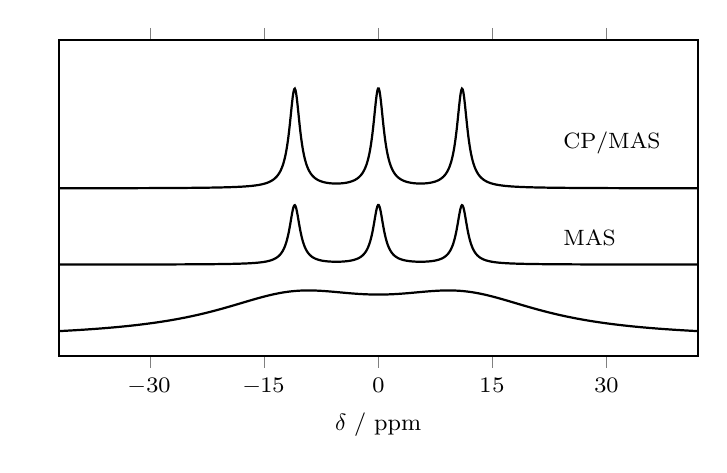
\begin{tikzpicture}
\tikzset{declare function={lor(\x,\c,\w)=1/(1+((\x-\c)/\w)^2);}}
\begin{axis}[
  width=\onecolwidth, height=56mm,
  xmin=-42, xmax=42, ymin=-0.4, ymax=7.9,
  xtick={-30,-15,0,15,30}, ytick=\empty,
  xlabel={$\delta$ / ppm}, ylabel={信号强度（任意单位）},
  axis line style={black}, tick align=outside,
  every axis plot/.append style={thick},
  samples=900
]
\addplot[black,domain=-42:42]{0.05+1.00*lor(x,-11,13)+1.00*lor(x,11,13)};
\node[anchor=west,text width=15mm,align=left,font=\fontsize{8}{9.6}\selectfont]
  at (axis cs:23,0.75){静态粉末谱};
\addplot[black,domain=-42:42]{2.00+1.55*lor(x,-11,0.85)+1.55*lor(x,0,0.85)+1.55*lor(x,11,0.85)};
\node[anchor=west,text width=15mm,align=left,font=\fontsize{8}{9.6}\selectfont]
  at (axis cs:23,2.70){MAS};
\addplot[black,domain=-42:42]{4.00+2.60*lor(x,-11,0.85)+2.60*lor(x,0,0.85)+2.60*lor(x,11,0.85)};
\node[anchor=west,text width=15mm,align=left,font=\fontsize{8}{9.6}\selectfont]
  at (axis cs:23,5.20){CP/MAS};
\end{axis}
\end{tikzpicture}
\caption{同一组三条共振线的增宽与窄化对照（自下而上：静态粉末谱、MAS 谱、CP/MAS 谱）。
读者应看三点：静态谱因化学位移各向异性与偶极作用连成一片宽包；MAS 把它收成三条窄线，
但峰高受灵敏度限制；CP/MAS 在同样线宽下信号大幅增强。本图按洛伦兹线型计算的示意图，
不是任何具体样品的实测谱，纵轴为任意单位，三条谱线按竖直方向错开以便比较。
\schemamark\figsrc{据 S2 §8.1.2--§8.1.3，书内 p.529—530 / PDF p.21—22 的原理绘制。}}
\label{fig:mas-compare}
\end{figure}

\subsubsection{$^{27}$Al MAS NMR 研究}

$^{27}$Al 是骨架的另一个关键核，天然丰度 100\%，化学位移总范围约 450 ppm，分子筛多数在
100 ppm 内。$^{27}$Al 是 $I=5/2$ 的四极核：由于固体中的四极相互作用，只有
$(+1/2\leftrightarrow-1/2)$ 中心跃迁可以观测到，该跃迁的线形畸变与位移不受一阶相互作用
影响，仅由二阶相互作用决定；其他允许跃迁因谱线太宽、位移太远而无法直接观测。
\textbf{四极作用引起的增宽与磁场强度成反比}，故高场加快速旋转才能得到高质量的
$^{27}$Al MAS 谱；要得到定量可靠的结果，还须采用扳倒角小于 $10^\circ$ 的强射频脉冲。
同一 Y 型分子筛在 \qty{23.45}{MHz} 与 \qty{104.22}{MHz} 下的谱对比表明，高场获得的谱线
更窄、畸变更小——但即使如此，MAS 也只能大幅减小而\textbf{一般不能完全消除}四极相互作用。
结构完整的沸石分子筛中铝的环境均为 Al(4Si)，四面体铝只在 50--65 ppm 出现单个共振峰；
$^{27}$Al 化学位移对不同配位的铝物种十分敏感，因此可据此区分四配位骨架铝与 0 ppm 附近的
六配位非骨架铝。\src{S2 §8.2.2，书内 p.534—535 / PDF p.26—27}

脱铝过程提供了这套判据的典型用法：结构规整的 Y 型分子筛只在 58 ppm 左右出现一个四配位
骨架铝峰；与 SiCl$_{4}$ 反应后骨架铝峰大大降低，同时在 0 ppm 左右出现八面体非骨架铝峰，
并在 100 ppm 处出现一个很强的峰，归属为高温反应生成的 NaCl 与 AlCl$_{3}$ 进一步生成的
Na[AlCl$_{4}$]；经水洗除去 Na[AlCl$_{4}$] 后 100 ppm 峰消失，但更多非骨架铝沉积在孔道中，
0 ppm 峰增强；再经多次水洗或离子交换可除去孔道中大量非骨架铝。水洗后谱线的宽化说明铝物种
环境的\textbf{不对称性增加}：$^{27}$Al 谱的线宽主要取决于核四极耦合常数
$C_{Q}=e^{2}qQ/h$（$q$ 为电场梯度张量的 $z$ 分量，$eQ$ 为核四极矩）与不对称因子 $\eta$，
高度不对称的环境会使谱线严重增宽，直至一些 $^{27}$Al 信号难以被观测到。
\src{S2 §8.2.2，书内 p.536 / PDF p.28}

\begin{pitfall}
\textbf{「看不见」不等于「不存在」。}这是 $^{27}$Al MAS NMR 最容易出错的一处：当铝落进
高度不对称的配位环境时，二阶四极增宽可把信号摊到极宽的频率范围内，中心带峰高降到噪声
以下而被判为「无铝」。正确做法是先用高场、高速 MAS 与回波（或 MQ MAS）确认信号是否真的
不存在，再下结论；把「未观测到」直接写成「不含该物种」，会把结构结论建立在仪器条件上。
\src{S2 §8.2.2，书内 p.536 / PDF p.28}
\end{pitfall}

\subsubsection{$^{17}$O MAS NMR 研究}

$^{17}$O 与 $^{27}$Al 一样是 $I=5/2$ 的四极核，但天然丰度只有 0.037\%，通常必须做
$^{17}$O 富集。$^{17}$O MAS NMR 谱\textbf{同时受化学位移各向异性与核四极矩的影响}，这一
双重性正是它的信息价值所在。A 型分子筛中 $^{17}$O 只有 Si--$^{17}$O--Al 结构，其谱峰显示
较小的四极作用特征；而高硅 Y 型分子筛中 $^{17}$O 只含 Si--$^{17}$O--Si 结构，却显示一定
的四极相互作用。Si/Al 比为 2.74 的 NaY 分子筛，其 $^{17}$O 静态谱与 MAS 谱都可以由
Si--$^{17}$O--Si 和 Si--$^{17}$O--Al 两个组分模拟；由这两个组分的峰面积即可计算 Si/Al 比，
且这样得到的\textbf{仅仅是骨架中的} Si/Al 比——这是 $^{17}$O 相对于 $^{29}$Si 与化学分析
的独特之处。\src{S2 §8.2.3，书内 p.536 / PDF p.28}

半整数四极核（$^{23}$Na、$^{27}$Al、$^{17}$O 等）的研究兴趣推动了多种消除二阶四极作用的
技术：二维章动谱、变角实验、动态变角（DAS）、双旋转（DOR）与多量子谱等。其中 MQ MAS 比
DOR、DAS 简单得多，不需要特殊硬件，特别适用于自旋--晶格弛豫时间短和四极耦合常数较小的核。
多量子 MAS 实验通常用一个简单的二脉冲序列得到二维谱，通过相位循环选择三量子或五量子
跃迁，得到 3Q MAS 或 5Q MAS 谱。以 $^{17}$O 富集的 Na-ZSM-5 的二维 $^{17}$O 3Q MAS 谱
为例：F2 域投影就是常规一维 $^{17}$O MAS 谱，两个相关峰表明存在两种不同的 $^{17}$O 物种；
F1 域投影出现两个分离峰，可直接读出两种物种的各向同性化学位移分别为 50 ppm
（Si--O--Si）与 33 ppm（Si--O--Al），NQCC 分别为 5.3 MHz 与 3.5 MHz，$\eta$ 为 0.12 与
0.29；再据这些四极参数模拟一维 MAS 谱，得到两种物种的浓度分别为 80\% 与 20\%。MQ MAS 的
主要局限是\textbf{不适宜研究四极相互作用很大的物种}。
\src{S2 §8.2.3，书内 p.537—538 / PDF p.29—30}

\subsubsection{$^{31}$P MAS NMR 研究}

$^{31}$P 的 $I=1/2$，天然丰度 100\%，是很适宜 NMR 研究的灵敏丰核。含磷的磷酸铝分子筛
（如 AlPO$_{4}$-11）及含 P、Si、Al 的 SAPO 类分子筛，除研究其 $^{29}$Si 与 $^{27}$Al 谱外，
还可用 $^{31}$P MAS NMR 研究结构变化。VPI-5 的原位变温 $^{31}$P MAS NMR 谱是一个干净的
例子：室温下 VPI-5 有三个强度比 1:1:1 的 $^{31}$P 峰，对应空间群 P6$_{3}$ 结构中三个
占有率为 1:1:1 的 P 结构位；随温度升高，三个峰最终变为强度比 2:1 的两个峰，对应空间群
P6$_{3}$cm 结构中两个占有率为 2:1 的 P 结构位。峰的数目与强度比直接读出结构位的数目与
占有率，这正是 $^{31}$P MAS NMR 在磷酸铝体系中的主要用法。
\src{S2 §8.2.4，书内 p.538 / PDF p.30}

\subsubsection{$^{47,49}$Ti MAS NMR 研究}

$^{49}$Ti 的 $I=7/2$、天然丰度 5.51\%；$^{47}$Ti 的 $I=5/2$、天然丰度 7.28\%。两者的
丰度都不算低，但有很大的四极相互作用，谱线极宽，且属于低频共振核：在 9.4 T 磁场下
$^{47}$Ti 与 $^{49}$Ti 的共振频率分别为 22.547 MHz 与 22.552 MHz。钛硅分子筛 TS-1 与
ETS-10 是两类受关注的材料，TS-1 为高硅 MFI 型分子筛，骨架中有 0.1\%--2.5\% 的 Si 被 Ti
取代；ETS-10 为大孔分子筛。SrTiO$_{3}$ 的 $^{49}$Ti 与 $^{47}$Ti 分别给出 $-864$ ppm 与
$-1133$ ppm 两条较窄的峰，说明其钛的四极相互作用较小；TS-1 与 ETS-10 则分别在 34 ppm
与 67 ppm 出 $^{49}$Ti 峰，由于存在很强的四极相互作用，谱峰很宽、灵敏度很低，均需几十万
次累加才能得到可用的 Ti MAS NMR 谱。\src{S2 §8.2.5，书内 p.539 / PDF p.31}

\begin{dataflow}
\textbf{从一张 MAS 谱到一条结构结论。}（1）\textbf{确认采集条件}：定量结论要求弛豫延迟
足够长（$^{29}$Si 的 $T_1$ 长，尤其如此），四极核定量还要求小扳倒角脉冲；谱是 CP/MAS 时
只能谈存在性，不能谈比例。（2）\textbf{定标}：用公认参比确定化学位移零点，跨磁场比较时
须用同一参比。（3）\textbf{归属}：先按化学位移分区（如 $^{27}$Al 的 50--65 ppm 四配位 /
0 ppm 六配位），再用已知结构样品校核分界值。（4）\textbf{定量}：分峰拟合求面积，并检查
旋转边带是否已全部计入。（5）\textbf{换算}：把面积转成结构量，如用式~\eqref{eq:sial}
得骨架 Si/Al 比、用 $^{17}$O 两组分面积得骨架 Si/Al 比。（6）\textbf{回查}：把结果与独立
方法对照（见下）。任何一步缺失，都不应把数字写成结构结论。
\src{S2 §8.2.1--§8.2.5，书内 p.531—539 / PDF p.23—31}
\end{dataflow}

\begin{crosscheck}
\textbf{互补与回查。}固体 NMR 给的是局域信息，必须与其它方法互查才能得到完整的结构图像：
（i）与 \textbf{XRD} 互补——XRD 给长程有序的晶体结构与结晶度，NMR 给局部配位；短程有序
或非晶态材料中后者仍有效。（ii）与\textbf{化学分析}互补——式~\eqref{eq:sial} 给出骨架
Si/Al 比，化学分析给出总 Si/Al 比，两者之差即非骨架铝的量，这一差值是判断脱铝程度的
常用依据。（iii）\textbf{多核互查}——$^{29}$Si 看硅的分布与 Si/Al 比，$^{27}$Al 看骨架铝
与非骨架铝的区分，$^{17}$O 给出骨架 Si/Al 比与氧的四极参数，$^{31}$P 用于磷酸铝体系，
$^{47,49}$Ti 用于钛硅材料；同一份样品上若 $^{29}$Si 给出的骨架 Si/Al 比与 $^{17}$O 不
一致，应先怀疑定量条件（弛豫延迟、边带、脉冲扳倒角），而不是直接采信任一方。
（iv）与\textbf{红外、NH$_3$ 程序升温脱附}等在酸性表征上互查（见后文酸性表征部分）。
\src{S2 §8.1--§8.2，书内 p.527—539 / PDF p.19—31}
\end{crosscheck}
}{}
\IfFileExists{chapters/parts/ch08-b.tex}{% ================================================================
%  chapters/parts/ch08-b.tex   （第 8 章 核磁共振方法，分片 b）
%  源：S2（下册）第 8 章，书内 p.540—550 / PDF p.32—42
%  覆盖：8.3 固体 NMR 在催化剂酸性研究中的应用（8.3.1—8.3.3）
%        8.4 催化剂表面吸附分子的 NMR 研究（8.4.1 孔道内有机物；8.4.2 129Xe）
%  未覆盖（分片 c）：8.5 原位 MAS NMR、8.6 积炭（8.4.2 第 5 小节的积炭细节亦在彼处）
%  页码说明：下册印刷页 526 未出现在 PDF 中，书内页码跳号属正常，一律以分片源文
%            的 [[DOWN PDF p.n | 书内 p.m]] 标记为准。
%  注：本分片源文 OCR 层\textbf{系统性丢失负号}（如 −68 记作 68）。凡负号均按上下文
%      （物理吸附 TMP 应在高场、L 酸络合物在 −60～−32 区间）恢复，并在相应位置用
%      \tocheck 标明"符号系恢复"，供集中核验。
% ================================================================

\subsection{固体 NMR 在催化剂酸性研究中的应用}
\label{sec:acidity}

\begin{probout}
本节要输出四个彼此独立的量：\textbf{酸的类型}（B 酸还是 L 酸）、\textbf{酸强度}、
\textbf{酸密度}（中心数目）与\textbf{可接近性}（酸性位在内表面还是外表面）。与常用方法相比，
红外光谱受消光系数制约，把吸收峰强度换算成基团数目存在系统性困难，峰重叠又使分辨率下降；
\ce{NH3} 程序升温脱附（\ce{NH3}-TPD）测的是脱附行为，\textbf{分辨不了酸的类型}。固体 NMR 有
两条入口：一是用 $^{1}$H MAS NMR 直接看桥羟基（B 酸位）；二是先让探针分子
（\ce{(CH3)3P}、\ce{^{15}N}-吡啶、\ce{^{13}CO} 等）吸附，再测探针核的化学位移。后者不仅
能区分酸的类型、强度与密度，借助\textbf{不同尺寸}的探针分子还能获得酸性位的空间信息。
\src{S2 §8.3，书内 p.540 / PDF p.32}
\end{probout}

\begin{principle}
\textbf{用碱性探针测酸强度的统一逻辑}是一条三步因果链：

\begin{center}
\fontsize{9}{13}\selectfont
碱的孤对电子（或 $\pi$ 体系）与酸位成键／成氢键 $\rightarrow$ 被观测核周围电子云被拉走
（去屏蔽）$\rightarrow$ 化学位移向\textbf{低场}（$\delta$ 增大）移动，\textbf{位移量随相互作用
强度单调增加}
\end{center}

由此得到三条使用纪律。（i）\textbf{位移是相对标尺，不是绝对酸强度}：只有\emph{同一探针、
同一参考态、同一温度}下的位移才能相互比较，标尺必须用一组酸强度已知的固体（SAPO-5、
HY、HZSM-5、HZSM-22 直到 \ce{AlCl3}/100\% \ce{H2SO4}、\ce{SbF5}）标定。（ii）\textbf{位移只
报告探针访问得到的酸位}：进不去孔道的探针不产生信号——这既是漏检的风险，也是可以选择
探针尺寸、只测外表面的手段。（iii）\textbf{位移给强度，峰面积给数目}，两者的成立条件不同，
后者的门槛见 8.3.3 的定量纪律。
\end{principle}

\subsubsection{$^{1}$H MAS NMR：不用探针的直接法}
\label{sec:h1-acidity}

分子筛的 Brönsted 酸位与骨架桥式羟基（Si—OH—Al）相关联，因此 $^{1}$H MAS NMR 是研究
表面 B 酸位\textbf{最直接}的方法——不需要引入任何探针分子，也就不存在"探针进不去孔道"
的问题。代价是固体中质子偶极--偶极作用很强、质子的化学位移范围又小，谱线极宽。可用的
窄化手段有：高速魔角旋转、特殊脉冲序列（如 \term{CRAMPS}{combined rotational and
multiple-pulse spectroscopy}{联合旋转与多脉冲谱}）、用 $^{2}$H 同位素稀释表面质子，以及
对催化剂表面做充分预处理。\src{S2 §8.3.1，书内 p.540 / PDF p.32}

\begin{measure}
\textbf{装样方式决定了能跑多快，也决定了谱可不可信。}酸性研究前样品必须\textbf{真空脱水}，
再装入转子或吸附探针。早期用玻璃封管法：催化剂在真空系统中抽空、吸附气体后用火焰密封，
制成小安瓿；玻璃管很难做得均匀对称，装入转子后转速一般低于 \qty{4}{kHz}。Haw 等设计的
\term{CAVERN}{}{原位处理装样装置}把催化剂平铺在床层上，使加热脱水和吸附都均匀进行，装样
后通过连杆密封转子，能有效防止装样时引入水，并允许较高转速；类似功能的装置用捣杆原位
装样、支架帽密封，转子最高转速可达 \qty{12}{kHz}。\src{S2 §8.3.1，书内 p.540 / PDF p.32}
\end{measure}

分子筛表面 OH 基的 $^{1}$H 化学位移归属如下（\src{S2 §8.3.1，书内 p.541 / PDF p.33}）：

\begin{itemize}[leftmargin=1.6em,itemsep=1pt,topsep=2pt]
\item $0.5\sim-0.5$ ppm：分子筛外表面或游离于骨架外、与金属离子相连的羟基（M—OH）；
\item $1.2\sim2.2$ ppm：缺陷位或端基硅羟基（Si—OH）；
\item $2.8\sim3.6$ ppm：与骨架铝相连、并与周围氧形成氢键的非骨架铝羟基（Al—OH）；
\item $3.6\sim4.3$ ppm：位于大笼或孔道中的桥式羟基（Si—OH—Al），即主 B 酸位；
\item $4.6\sim5.2$ ppm：位于八面沸石型分子筛小笼中的桥式羟基；
\item $5.2\sim7.0$ ppm：HZSM-5 与 H$\beta$ 中与骨架有静电作用的\textbf{第二种}桥式羟基。
\end{itemize}

\begin{principle}
\textbf{位移与红外波数之间的经验关系。}Brunner 把 $^{1}$H 化学位移 $\delta_{\mathrm{H}}$ 与该
OH 基在红外谱中的伸缩振动波数 $\nu_{\mathrm{OH}}$ 关联起来，给出两个经验式
（\src{S2 §8.3.1，书内 p.541 / PDF p.33}）：

\begin{equation}
\label{eq:brunner-iso}
\delta_{\mathrm{H}}\ (\mathrm{ppm})=57.1-0.0147\,\nu_{\mathrm{OH}}\ (\mathrm{cm^{-1}})
\qquad \text{（孤立 OH）}
\end{equation}

\begin{equation}
\label{eq:brunner-hb}
\delta_{\mathrm{H}}\ (\mathrm{ppm})=37.9-0.0092\,\nu_{\mathrm{OH}}\ (\mathrm{cm^{-1}})
\qquad \text{（存在氢键的 OH）}
\end{equation}

两式都写成"截距 $-$ 斜率 $\times\nu_{\mathrm{OH}}$"：波数越低（氢键越强、O—H 越弱），
$\delta_{\mathrm{H}}$ 越大，即向低场移动。\emph{核对说明}：已对照原页面图像
（书内 p.541 / PDF p.33），原书式（8-3）（8-4）逐字印作
$\delta_{\mathrm{H}}\,(\mathrm{ppm})=57.1-0.0147\,\nu_{\mathrm{OH}}\,(\mathrm{cm^{-1}})$、
$\delta_{\mathrm{H}}\,(\mathrm{ppm})=37.9-0.0092\,\nu_{\mathrm{OH}}\,(\mathrm{cm^{-1}})$，
减号、斜率与有效位数均与此处一致（源 OCR 文本层丢失了减号）。原书同时指出：
对与 Mg$^{2+}$、Ca$^{2+}$ 等金属离子相连的 OH，两式有偏差。
\end{principle}

\pedset{教学补充的自洽性核算（非原书数据）：把 HZSM-5 桥羟基的红外波数
$\nu_{\mathrm{OH}}\approx\qty{3610}{cm^{-1}}$ 代入式~\eqref{eq:brunner-iso}，得
$\delta_{\mathrm{H}}\approx4.0$ ppm，与上表 $3.6\sim4.3$ ppm 的桥羟基归属自洽；把原书提到
的 $\qty{3250}{cm^{-1}}$ 宽带代入式~\eqref{eq:brunner-hb}，得 $\delta_{\mathrm{H}}\approx8.0$ ppm，
与原书记录的 7.0 ppm 宽峰相差约 1 ppm——原书称"两个值能很好地符合"，读者可用同一组
公式复核这一对的偏差量。}

\begin{dataflow}
\textbf{从"看不见的铝"到脱羟基机制。}Freude 等对 HNaY 脱羟基过程做 $^{1}$H 与 $^{27}$Al
MAS NMR 定量，结果是桥羟基浓度的降低量与四配位骨架铝的减少量\textbf{相等}；这与
Uytterhoeven 等提出的"两个桥羟基缩合脱水生成一个骨架三配位铝"的模型不符。邓风等在不同
温度焙烧的 HZSM-5 上进一步发现两种脱羟基机制并存：一部分脱羟基伴随脱铝，另一部分只脱
羟基而不脱铝——后者的铝仍留在骨架上，但四极作用增强而变得"不可观测"。
\src{S2 §8.3.1，书内 p.541—542 / PDF p.33—34}
\end{dataflow}

\begin{crosscheck}
上一条的关键推论是：\textbf{谱上看不见的铝不等于不存在的铝}。因此任何"骨架铝含量"或
"B 酸位数目"的结论都必须回查三件事：（i）同一批样品的 $^{27}$Al MAS NMR 是否同时记录了
四配位、五配位、六配位铝，并说明定量用的是直接极化还是高功率去偶；
（ii）$^{1}$H MAS NMR 的桥羟基积分是否在全弛豫条件下获得（见 8.3.3）；
（iii）脱水／焙烧温度是否与比较样品一致，因为脱羟基程度本身就是温度的函数。三者缺一，
"酸量随温度下降"这类结论就可能只是"铝变不可观测"的假象。
\end{crosscheck}

\subsubsection{酸强度测定：探针分子的低场位移标尺}
\label{sec:acid-strength}

\textbf{强碱探针：吡啶。}强碱性分子氘代吡啶吸附后能有效区分酸性 OH 与非酸性 OH：吡啶与
Si—OH 形成氢键络合物时，其 $^{1}$H 化学位移由 2.0 ppm 移到约 10 ppm；而与桥羟基作用
生成质子化吡啶（吡啶阳离子）时移向更低场，落在 $15.5\sim19.5$ ppm 之间。
\src{S2 §8.3.2，书内 p.542 / PDF p.34}

\textbf{弱碱探针：位移本身就是酸强度的刻度。}不同碱性的吸附分子使桥羟基产生不同的低场
位移。在 \qty{123}{K} 低温下，Haw 等观察到乙烯吸附在 HZSM-5 上使桥羟基向低场位移
2.7 ppm，相同条件下 CO 与乙烷分别只位移 1.8 ppm 与 0.6 ppm。
\src{S2 §8.3.2，书内 p.542 / PDF p.34}

\paragraph{丙酮-2-$^{13}$C：把 B 酸强度做成一条连续刻度。}
Biaglow 等在 \qty{125}{K} 下测定了丙酮-2-$^{13}$C 吸附在多种分子筛上的 $^{13}$C MAS NMR 谱。
在\textbf{每个桥羟基吸附一个丙酮分子}的条件下，相对于纯丙酮分子，羰基 $^{13}$C 的低场位移为：
SAPO-5 上 10.1 ppm，HY 上 12 ppm，HZSM-5 上 15 ppm，HZSM-22 上 18.7 ppm；在 \ce{AlCl3} 与
100\% \ce{H2SO4} 上位移 37 ppm，在 \ce{SbF5} 上位移 42 ppm。\textbf{酸性越强，羰基的 $^{13}$C
化学位移越移向低场}，因此这一方法可把分子筛 B 酸位的强度放在一条从弱到超强的连续刻度上
（图~\ref{fig:acetone-shift}）。\src{S2 §8.3.2，书内 p.542 / PDF p.34}

\begin{figure}[htbp]
\centering
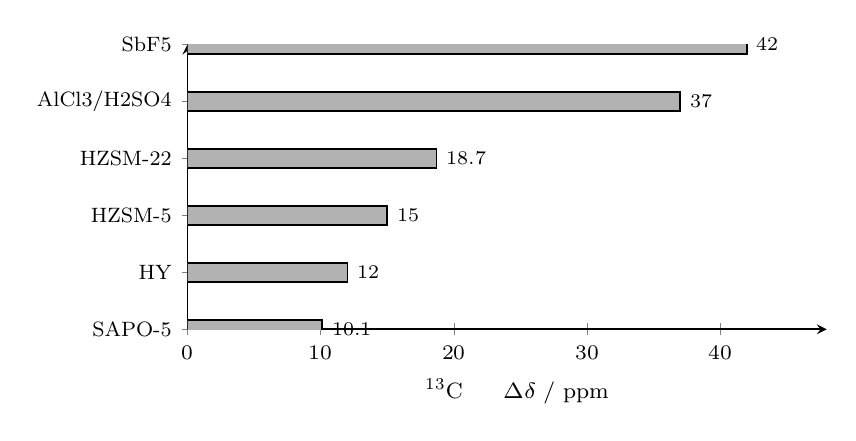
\begin{tikzpicture}
\begin{axis}[
  width=\onecolwidth, height=52mm,
  xbar, bar width=2.4mm,
  xmin=0, xmax=48,
  xlabel={羰基 $^{13}$C 低场位移 $\Delta\delta$ / ppm},
  xlabel style={font=\fontsize{8}{9.5}\selectfont},
  symbolic y coords={SAPO-5,HY,HZSM-5,HZSM-22,AlCl3/H2SO4,SbF5},
  ytick=data,
  y tick label style={font=\fontsize{7.5}{9}\selectfont},
  x tick label style={font=\fontsize{7.5}{9}\selectfont},
  nodes near coords,
  nodes near coords style={font=\fontsize{7}{8.5}\selectfont},
  enlarge y limits=0.10,
  axis lines=left,
]
\addplot[fill=black!30, draw=black] coordinates {
  (10.1,SAPO-5) (12,HY) (15,HZSM-5) (18.7,HZSM-22)
  (37,AlCl3/H2SO4) (42,SbF5)};
\end{axis}
\end{tikzpicture}
\caption{吸附丙酮-2-$^{13}$C 的羰基 $^{13}$C 低场位移，即一条 B 酸强度刻度。读者应看两点：
纵轴自下而上酸强度递增，位移量单调增大；分子筛区间（10.1—18.7 ppm）只占全刻度的前一半，
\ce{AlCl3}／100\% \ce{H2SO4} 与 \ce{SbF5} 把刻度延伸到 42 ppm。条件与局限：\qty{125}{K}、
每桥羟基覆盖一个丙酮分子，位移以纯丙酮为参考态；柱子为原书数据的重绘，未含误差棒。
\redrawmark\figsrc{据 S2 §8.3.2，书内 p.542 / PDF p.34 的数据改绘。}}
\label{fig:acetone-shift}
\end{figure}

\textbf{膦类探针。}吸附三甲基膦（trimethyl phosphine，TMP）与三甲基氧膦（trimethyl
phosphine oxide，TMPO）的 $^{31}$P MAS NMR 化学位移对 B 酸强度同样敏感：
\textbf{B 酸强度越强，$^{31}$P 化学位移越移向低场}。$^{31}$P 的天然丰度 100\%、磁旋比高，
不需要同位素富集，也不必用 CP/MAS，这一点对定量尤其重要（见 8.3.3）。
\src{S2 §8.3.2，书内 p.542 / PDF p.34}

\paragraph{用探针尺寸换取空间信息：全氟丁胺只测外表面。}
把探针分子做大，可以让它\textbf{只能}接触外表面。全氟丁胺
［\ce{(n-C4F9)3N}］的分子直径 0.94 nm，远大于 ZSM-5 的孔径 0.55 nm，因此只能吸附在分子筛
外表面。吸附后 $^{1}$H MAS NMR 谱中 3.9 ppm 处的 B 酸峰强度明显降低，而 6.0 ppm 处的
峰强有所增加——后者来自外表面 B 酸被质子化后向低场位移。由此可以\textbf{通过定量拟合吸附
前后 3.9 ppm 峰的积分面积，算出外表面的 B 酸含量}，同法可算外表面非骨架铝的含量。该实验
还发现吸附全氟丁胺后硅羟基一律向低场位移 $0.2\sim0.3$ ppm，据此推断\textbf{大部分硅羟基位于
分子筛外表面}。\src{S2 §8.3.2，书内 p.542 / PDF p.34}

\begin{dataflow}
上述实验的逻辑链值得单独记住，因为它把"化学位移"与"空间位置"接了起来：

尺寸排斥（探针 0.94 nm $>$ 孔口 0.55 nm）$\rightarrow$ 探针只能到达外表面 $\rightarrow$
只有外表面酸位被质子化 $\rightarrow$ 3.9 ppm 峰\textbf{面积减少量} $=$ 外表面 B 酸量 $\rightarrow$
与总量相减得内表面 B 酸量。注意最后一个箭头依赖一个前提：\textbf{3.9 ppm 峰的减少全部来自
外表面}。若探针能部分进入孔口（例如分子筛有缺陷、介孔或堆积孔），这个前提就被破坏，得到
的"外表面酸量"会被高估。\src{S2 §8.3.2，书内 p.542—543 / PDF p.34—35}
\end{dataflow}

\begin{pitfall}
\textbf{把化学位移直接当作酸强度。}这是本小节最常见、也最难自查的误判，至少有四个来源：
（i）\textbf{参考态漂移}——所有位移都是相对于某个参考态报出的（纯丙酮、液态吡啶、气相
Xe、液态 TMP），换参考态数值整体平移，而排序不变；（ii）\textbf{覆盖度与共吸附物}——丙酮
的位移刻度必须在"每个桥羟基一个丙酮分子"下读取，覆盖度变化或体系残留水都会改变氢键网络，
使位移偏离标定曲线；（iii）\textbf{温度}——弱碱探针的位移刻度依赖低温（\qty{123}{K}、
\qty{125}{K}）冻结交换，室温测量会把不同酸位的信号平均成一条线；（iv）\textbf{孔道限域效应}
——同样的酸位在窄孔中与被质子化探针的构象、取向受约束，$^{31}$P 位移还包含探针本身形变
的贡献。正确做法是：\textbf{在同一次实验、同一参考态、同一温度下测一系列酸强度已知的样品，
用相对次序说话}，并把探针覆盖度写进结论的条件里。
\end{pitfall}

\subsubsection{区分与计数 B 酸／L 酸中心：探针选择与定量纪律}
\label{sec:bl-quant}

\textbf{L 酸只能靠探针。}用 NMR 研究 L 酸性质时没有"直接法"，必须引入探针分子，而且大部分
探针需要同位素标记；好在一般探针既能研究 L 酸，也能同时区分 B 酸。
\src{S2 §8.3.3，书内 p.543 / PDF p.35}

\textbf{\ce{^{13}CO}：L 酸中心的探针，但读不直接。}吸附 CO 的 $^{13}$C 化学位移与其气态相差
很大，可用来探测固体表面的 L 酸中心；然而无论在室温还是低温下，吸附在 L 酸上的 CO 与
物理吸附的 CO、吸附在 B 酸位上的 CO 之间\textbf{都存在交换}，因此谱图上无法直接读出 L 酸位
上 CO 的化学位移，需要\textbf{通过计算}才能获得；该位移落在 $300\sim400$ ppm 之间。
\src{S2 §8.3.3，书内 p.543 / PDF p.35}

\textbf{\ce{^{15}N}-吡啶：位移范围大，但要富集。}Maciel 等对无定形硅铝上 \ce{^{15}N}-吡啶的
\ce{^{15}N} CP/MAS NMR 谱作如下归属：B 酸位上吸附的吡啶在约 205 ppm；L 酸位上的约在
260 ppm；吸附在弱酸位羟基上形成氢键的在 $290\sim300$ ppm；液态吡啶在 315 ppm。$^{15}$N 的
优点是化学位移范围大、各类酸中心容易分开，缺点是天然丰度低，必须同位素富集。
\src{S2 §8.3.3，书内 p.543 / PDF p.35}
\emph{核对说明}：已对照原页面图像（书内 p.543 / PDF p.35），该组数值逐字一致——B 酸位上
吸附吡啶的 \ce{^{15}N} 在 205 ppm 左右、L 酸位上的约在 260 ppm 处、弱酸位羟基上形成氢键的
在 $290\sim300$ ppm、液态吡啶在 315 ppm；原书\textbf{未随数值给出参考标准}（液氨、硝基甲烷等），
跨文献比较前须自行确认参考态。

\paragraph{三甲基膦 TMP：一个探针同时给出 B 酸与 L 酸两个窗口。}
Lunsford 等首先研究了 TMP 在 HY 分子筛上的 $^{31}$P MAS NMR 谱，得到三个分区
（\src{S2 §8.3.3，书内 p.543—544 / PDF p.35—36}）：

\begin{itemize}[leftmargin=1.6em,itemsep=1pt,topsep=2pt]
\item $-3\sim-1$ ppm：TMP 与 B 酸位形成的 \ce{(CH3)3PH+}；
\item $-60\sim-32$ ppm：TMP 与 L 酸位形成的络合物；
\item 约 $-68$ ppm：物理吸附的 TMP。
\end{itemize}

\emph{核对说明}：已对照原页面图像（书内 p.543 / PDF p.35），原书三处数值\textbf{均带负号}
印作 $-3\sim-1$ ppm（\ce{(CH3)3PH+}）、$-60\sim-32$ ppm（TMP–L 酸络合物）、$-68$ ppm 左右
（物理吸附 TMP），与本分片一致；源 OCR 文本层丢失了这些负号，此前据物理次序的恢复方向正确。

这一分区方式带来两个后果，一正一反：\textbf{B 酸位的膦峰远离其他膦峰，因此可以直接测定
表面 B 酸中心的数目}；而\textbf{L 酸络合物峰与物理吸附峰彼此很靠近，故不易直接定量 L 酸的
中心数目}。Coster 等观察到 TMP 在超强酸 \ce{ZrO2}/\ce{SO4^{2-}} 上吸附时，除与 B 酸和 L 酸位
结合的共振峰外，$26$ ppm 处还出现一个强信号；与吸附苯胺后的 ESR 结果比较后，认为该峰
应为 TMP 与\textbf{超强 L 酸中心}的络合物。\emph{核对说明}：已对照原页面图像（书内 p.544 /
PDF p.36），原书此处印作「在 26 ppm 处还出现一个强信号」，\textbf{不带负号}，与本分片
$26$ ppm 的写法一致；与此前 $-60\sim-32$ ppm 的 L 酸络合物窗口相比，该峰更靠低场，
正与「超强 L 酸中心去屏蔽更强」相符。

\begin{figure}[htbp]
\centering
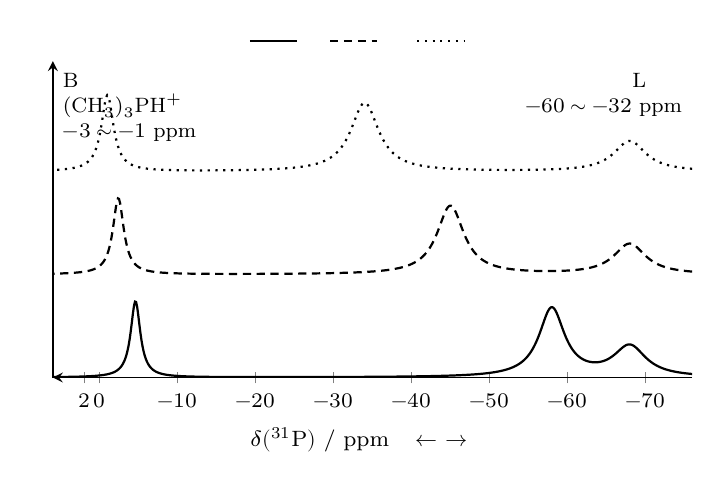
\begin{tikzpicture}
\tikzset{declare function={
  lor(\x,\p,\w) = 1/(1+((\x-\p)/\w)^2);
  spA(\x) = 1.00*lor(\x,-4.6,0.75) + 0.90*lor(\x,-58,2.0) + 0.40*lor(\x,-68,2.5);
  spB(\x) = 1.00*lor(\x,-2.4,0.85) + 0.90*lor(\x,-45,2.1) + 0.40*lor(\x,-68,2.5);
  spC(\x) = 1.00*lor(\x,-1.0,0.95) + 0.90*lor(\x,-34,2.2) + 0.40*lor(\x,-68,2.5);
}}
\begin{axis}[
  width=\onecolwidth, height=56mm,
  xmin=-76, xmax=6, x dir=reverse,
  ymin=0, ymax=4.15,
  xlabel={$\delta(^{31}\mathrm{P})$ / ppm（低场 $\leftarrow$ $\rightarrow$ 高场）},
  xlabel style={font=\fontsize{8}{9.5}\selectfont},
  ylabel={相对强度（叠加显示）},
  ylabel style={font=\fontsize{8}{9.5}\selectfont},
  axis lines=left, ytick=\empty,
  xtick={2,0,-10,...,-70},
  tick label style={font=\fontsize{7.5}{9}\selectfont},
  legend style={font=\fontsize{7.5}{9}\selectfont, draw=none, fill=none,
                legend columns=3, at={(0.5,1.02)}, anchor=south},
  samples=600, domain=-76:6,
]
\addplot[black, thick] {spA(x)};
\addplot[black, thick, densely dashed] {spB(x)+1.35};
\addplot[black, thick, dotted] {spC(x)+2.70};
\legend{弱酸位, 中等酸位, 强酸位}
\node[anchor=north west, align=left, text width=20mm,
      font=\fontsize{7.5}{9}\selectfont] at (axis cs:6,4.12)
      {B 酸位 \ce{(CH3)3PH+}\\ $-3\sim-1$ ppm};
\node[anchor=north east, align=right, text width=20mm,
      font=\fontsize{7.5}{9}\selectfont] at (axis cs:-76,4.12)
      {L 酸位络合物\\ $-60\sim-32$ ppm};
\end{axis}
\end{tikzpicture}
\caption{模型计算的吸附 TMP 的 $^{31}$P MAS NMR 谱：两条峰位随酸强度移动。读者应看两件事：
（i）每个酸强度下都有两组信号——左（低场）为 B 酸位上的 \ce{(CH3)3PH+}，右（高场）为 L 酸
位络合物；（ii）酸强度由弱到强（自下而上），\textbf{两组峰同时向低场移动}，B 酸峰由
$-4.6$ 移到 $-1.0$ ppm，L 酸峰由 $-58$ 移到 $-34$ ppm，而 $\approx-68$ ppm 的物理吸附峰
（图中最右的小峰）位置不随酸强度改变。条件与局限：曲线由洛伦兹线型叠加合成，峰位取自
原书给出的分区端点，线宽、相对强度与叠加偏置均为设定值，\textbf{不是实验谱}；真实谱中 L 酸
络合物峰与物理吸附峰相距很近、部分重叠，定量须做分峰拟合。\modelmark\figsrc{模型参数据
S2 §8.3.3，书内 p.543—544 / PDF p.35—36 的化学位移区间设定。}}
\label{fig:tmp-p}
\end{figure}

\begin{table}[htbp]
\centering
\footnotesize
\setlength{\tabcolsep}{1.5pt}
% 原五列合计仅 80 mm（版心 165 mm），最窄列装不下内容，单元格溢出 9.05 pt。
% 【重叠修正，2026-09-30】上一轮只加宽到 108 mm，仍空着 57 mm 版心；单元格被挤成
% 多行，表格连图题一起高出整页 —— 编译日志实测
%   `LaTeX Warning: Float too large for page by 37.14322pt on input line 361`，
% 浮动体被强行放下后**溢出到页脚**：图题最后两行落在 y=788—809，
% 而页脚页码 `158` 在 y=784.7—791.0，实测 5 对字形墨迹相交（最大 `表`×`5` 0.907 pt²）。
% 本轮把五列吃满版心（158 mm + 4×2×1.5 pt 列间距 ≈ 162 mm < 165 mm），
% 单元格行数随之下降，浮动体不再超高。列宽之和勿减，否则会再次触发上述警告。
\begin{tabular}{@{}p{20mm}p{12mm}p{30mm}p{40mm}p{56mm}@{}}
\toprule
探针分子 & 核种 & 测什么 & $\delta$ 区间 / ppm & 定量前提与主要干扰 \\
\midrule
\ce{(CH3)3P}（TMP）
 & \ce{^{31}P} & 同时给出 B 酸位与 L 酸位两个窗口 &
 B：$-3\sim-1$；\\ L：$-60\sim-32$；物理吸附 $\approx-68$ &
 丰度 100\%，不需富集、不需 CP/MAS；L 络合物峰与物理吸附峰靠近，须分峰 \\
\addlinespace[2pt]
\ce{^{15}N}-吡啶
 & \ce{^{15}N} & 区分 B 酸／L 酸／弱酸位 &
 B 205；L 260；\\ 弱酸 $290\sim300$；液态 315 &
 位移范围大、易分辨；天然丰度低，\textbf{必须同位素富集}，参考态须统一 \\
\addlinespace[2pt]
丙酮-2-$^{13}$C
 & \ce{^{13}C} & B 酸强度刻度 &
 相对纯丙酮的位移 $10.1\sim42$ &
 须"每桥羟基一个丙酮分子"、低温（\qty{125}{K}）；覆盖度与残水改变刻度 \\
\addlinespace[2pt]
\ce{^{13}CO}
 & \ce{^{13}C} & L 酸中心 &
 L 酸位 $300\sim400$（须计算求得） &
 室温与低温下 L 酸位、B 酸位、物理吸附的 CO 均在交换，谱上读不出，只能拟合 \\
\addlinespace[2pt]
吡啶-d$_5$
 & $^{1}$H & 区分酸性／非酸性 OH &
 氢键 $\approx10$；\\ 吡啶阳离子 $15.5\sim19.5$ &
 强碱优先占据最强酸位；须确认化学计量覆盖，否则高估强酸位数 \\
\addlinespace[2pt]
乙烯／CO／乙烷
 & $^{1}$H & 弱碱探针测桥羟基低场位移 &
 $+2.7$／$+1.8$／$+0.6$（\qty{123}{K}） &
 位移小，必须低温冻结交换；参考态误差与位移同量级，只宜作相对比较 \\
\addlinespace[2pt]
全氟丁胺
 & $^{1}$H & 外表面 B 酸与非骨架铝定量 &
 3.9 峰降、\\ 6.0 峰升（位移 $0.2\sim0.3$） &
 分子 0.94 nm $>$ 孔口 0.55 nm，只接触外表面；靠差减积分，前提是无介孔／缺陷漏入 \\
\addlinespace[2pt]
$^{1}$H（直接法）
 & $^{1}$H & 各类羟基的归属与桥羟基定量 &
 分六档，$0.5\sim7.0$ &
 须真空脱水、高速 MAS（或 CRAMPS）；残水与装样污染同时改变位移与强度 \\
\bottomrule
\end{tabular}
\caption{酸性探针分子对照。读者用法：先按"想测什么"选行，再核对同一行的"定量前提与
主要干扰"是否满足；表中位移均为相对各自参考态的数值，\textbf{不可跨探针直接比大小}。
条件与局限：区间取原书给出的端点，个位数与符号见正文各处的待核对标注。
\src{据 S2 §8.3.2—§8.3.3，书内 p.542—544 / PDF p.34—36 汇总。}}
\label{tab:probes}
\end{table}

\begin{principle}
\textbf{定量前提：小扳倒角 $+$ 足够长的弛豫延迟。}探针定量的目标是让\textbf{峰面积比等于
核数目比}。单脉冲实验中第 $n$ 次扫描的稳态信号为

\begin{equation}
\label{eq:ernst}
S\;\propto\;N\cdot\frac{\sin\alpha\,\bigl(1-e^{-D_1/T_1}\bigr)}
{1-\cos\alpha\,e^{-D_1/T_1}}
\end{equation}

式中 $N$ 为产生该峰的核数目，$\alpha$ 为扳倒角（射频脉冲宽度决定），$D_1$ 为弛豫延迟，
$T_1$ 为自旋--晶格弛豫时间。式~\eqref{eq:ernst} 说明两件事：（i）只要
$D_1\gtrsim5T_1$，指数项趋于零，$S\propto N\sin\alpha$，面积比即数目比——\textbf{弛豫延迟
不足时，$T_1$ 短的峰被相对放大，强度比失真}；（ii）当 $\alpha$ 小到
$\sin\alpha\approx\alpha$、$\cos\alpha\approx1$ 时，$D_1/T_1$ 项整体约掉，
$S\propto N\alpha$，\textbf{强度比对 $T_1$ 的差异不再敏感}。这就是"小扳倒角
（$\alpha\lesssim10°$）$+$ 强射频脉冲"的用处：它把定量从"必须等 5$T_1$"变成"不必等 5$T_1$"，
代价是灵敏度按 $\sin\alpha$ 下降，需要更多累加次数。\pedset{本式为 NMR 定量的通用关系，
是教学补充（原书未给该式）；原书给出的要求是定性表述——固体 NMR "在定量方面优于红外光谱"，
但 L 酸络合物峰与物理吸附峰靠近而"不易直接定量"（\src{S2 §8.3.3，书内 p.543—544 /
PDF p.35—36}）。}
\end{principle}

\begin{measure}
\textbf{做定量前必须逐条确认的六件事。}（i）\textbf{扳倒角}：改用 $\alpha\lesssim10°$ 的
小扳倒角（或用已知 $T_1$ 的模型化合物标定脉冲宽度），并保留强射频脉冲以覆盖全谱宽；
（ii）\textbf{弛豫延迟}：实测各峰的 $T_1$ 后取 $D_1\gtrsim5T_1$，$\alpha$ 很小且已验证稳态时
可按 $(1-\cos\alpha)T_1$ 量级放宽；（iii）\textbf{旋转边带}：把转速提高或把全部边带一并
积分，只积中心带会系统性低估；（iv）\textbf{探针化学计量}：确认吸附量对应"每酸位一个
探针分子"，过量探针会同时产生物理吸附峰；（v）\textbf{温度与交换}：弱碱探针必须在低温
（\qty{123}{K}、\qty{125}{K}）测，否则不同酸位的信号被交换平均；（vi）\textbf{分峰模型}：
L 酸络合物与物理吸附峰重叠时应报告拟合约束与误差，而不是给一个单点数值。
\end{measure}

\begin{pitfall}
\textbf{四个必须设防的误判。}
（1）\textbf{弛豫延迟不足导致定量错误。}这是本节最重要的判断纪律：探针分子与酸位结合后
运动性下降，$T_1$ 与物理吸附态、自由态可以相差一个数量级；用统一的短延迟采集，会把
$T_1$ 短的物种（常是物理吸附或弱结合态）算多，把强结合态算少，而"B 酸／L 酸数目比"恰恰
建立在这两类峰的面积比上。看到一篇文献给酸位数目而不给 $\alpha$、$D_1$、$T_1$，
就应当把它当作\textbf{定性}结果使用。
（2）\textbf{把化学位移直接当酸强度。}位移受参考态、覆盖度、温度与限域效应共同影响
（见 8.3.2 的误判框），只能在同一套标定条件下作相对比较。
（3）\textbf{探针分子太大进不去小孔，被误读为"没有酸位"。}探针尺寸既是优点也是陷阱：
0.94 nm 的全氟丁胺进不去 0.55 nm 的 ZSM-5 孔道，那是有意为之；但若用大尺寸探针去筛
小孔分子筛并据此宣布"孔内无酸性位"，就把\textbf{扩散限制}错当成了\textbf{无酸位}。
判据是：换一个尺寸小于孔口、化学性质相近的探针（如 TMP、\ce{NH3}）重测，若信号出现，
则原结论只是可接近性问题。分子筛中扩散慢是常态——源文在 \ce{^{129}Xe} 一节记录到，苯在
NaY／NaX 中室温扩散很慢，吸附 120 天后才出现多个分离的共振峰；\qty{523}{K} 加热 10 h 才
给出均匀分布的单峰（\src{S2 §8.4.2，书内 p.549—550 / PDF p.41—42}）。装样后的
\textbf{平衡时间}因此是探针实验的隐藏变量，必须与升温／抽空历史一并报告。
（4）\textbf{把旋转边带当成真实峰。}MAS 下只要转速不足以平均该核的各向异性，中心带两侧就
会出现间隔\textbf{恰好等于转速}的旋转边带；$^{31}$P 与 \ce{^{129}Xe} 的化学位移跨度大，
边带更容易落到"看起来像另一个酸位"的位置上，从而凭空多出一个"L 酸位"。判别办法只有一条：
\textbf{改变转速重测}——真实峰的位置不随转速移动，边带的位置随转速整体平移；此外可用
边带间隔直接反读转速自检。\src{S2 §8.3—§8.4，书内 p.543—546 / PDF p.35—38}
\end{pitfall}

\begin{crosscheck}
\textbf{酸性结论的交叉验证组合。}（i）$^{1}$H MAS NMR 的桥羟基积分（B 酸总量）与
$^{27}$Al MAS NMR 的四配位骨架铝含量互相校核，两者不等时先怀疑"铝变不可观测"，而不是
直接修改酸量结论；（ii）吡啶吸附红外（区分 B／L 酸的特征环振动）与 $^{15}$N-吡啶 NMR 互相
校核——红外给出类型与相对强度、NMR 给出可分辨的位移与数目；（iii）\ce{NH3}-TPD 的脱附峰温
给出强度分布的定性排序，与丙酮-$^{13}$C 的位移刻度对照，若排序矛盾，优先检查探针覆盖度与
平衡时间；（iv）外表面酸量的结论必须用不同尺寸探针（全氟丁胺 vs TMP）分别测量并给出
差值；（v）所有定量结论最终要写清 $\alpha$、$D_1$、转速、探针覆盖度与平衡时间四项
实验参数，否则不可复现。\src{S2 §8.3，书内 p.540—544 / PDF p.32—36}
\end{crosscheck}

源文对 NMR 测酸性的总体评价是：固体 NMR 已成为研究多相催化剂酸性的有力工具，能得到其他
方法难以得到的信息，\textbf{在定量方面优于红外光谱}；但在 L 酸研究方面一般需采用同位素
富集的探针分子，相比之下\textbf{三甲基膦不失为一个较好的 NMR 探针}。
\src{S2 §8.3.3，书内 p.544 / PDF p.36}

\subsection{催化剂表面吸附分子的 NMR 研究}
\label{sec:adsorbed}

研究催化剂表面吸附分子的化学性质以及催化反应中间产物的结构，是从分子水平阐明催化反应
机理的关键，NMR 已被广泛用于表面吸附分子状态与氢溢流的研究；多相催化过程在很大程度上
取决于反应物在催化剂表面的吸附行为，而惰性气体氙（Xe）是一种非常理想的探针分子，
\ce{^{129}Xe} NMR 已成为研究多孔物质、特别是分子筛结构的有效工具。
\src{S2 §8.4，书内 p.544 / PDF p.36}

\subsubsection{分子筛晶体孔道中吸附有机物的化学状态}
\label{sec:methanol}

\textbf{案例：甲醇在 HZSM-5 上的吸附与转化。}甲醇转化制烃是工业上有代表性的重要反应，
其机理（特别是第一个 C—C 键如何生成、甲醇与骨架如何相互作用）长期有争议。用
$^{1}$H MAS NMR 研究甲醇在 HZSM-5 上的吸附性质，得到的观察与推断可以分开陈述。
\src{S2 §8.4.1，书内 p.544—545 / PDF p.36—37}

\begin{obs}
甲醇吸附在 HZSM-5 上后，$^{1}$H MAS NMR 谱中出现 4.1 ppm 的甲基峰，OH 峰位于
9.1 ppm，比甲醇在 \ce{CDCl3} 中向低场位移 3.1 ppm；不论吸附的是 \ce{CD3OH}、\ce{CH3OD}
还是 \ce{CD3OD}，所有羟基的化学位移都在 9.1 ppm 左右。把覆盖度降到每个 B 酸位"只覆盖
两个甲醇分子"时，OH 信号由 9.1 ppm 移向 10.5 ppm。
\emph{核对说明}：已对照原页面图像（书内 p.544 / PDF p.36），4.1 ppm 甲基峰、9.1 ppm OH
峰、「比其在 \ce{CDCl3} 中向低场位移 3.1 ppm」、三种氘代样品羟基均在 9.1 ppm 左右、以及
「每个 B 酸只覆盖两个甲醇分子时 OH 由 9.1 ppm 移向 10.5 ppm」均逐字一致。两点说明：
原书\textbf{未印出} \ce{CDCl3} 中甲醇 OH 的具体位移，约 6.0 ppm 系由 $9.1-3.1$ 反推的本分片
推算值；原书原句为「当每个 B 酸\textbf{只}覆盖两个甲醇分子时」，对应的是\textbf{低覆盖}一侧。
\end{obs}

\begin{infer}
液体甲醇中 OH 之间已存在氢键，O—H 键的静电极化使其 $^{1}$H 去屏蔽；吸附到 HZSM-5 上后
出现如此大的低场位移，\textbf{必定来自很强的氢键和／或醇的质子化}。三种同位素取代样品的
OH 位移都在 9.1 ppm 附近，说明\textbf{所有 $^{1}$H 在 NMR 时域上是等价的}：在甲醇形成的
氢键中，端基甲醇分子与 B 酸位的桥氧形成氢键，每个甲醇分子中的甲氧基离子相同，这样一个
以氢键相连的带电簇可在孔道中转动，使羟基的 H 变成等价。覆盖度降低时 OH 由 9.1 移到
10.5 ppm，说明 B 酸位的 H 与吸附甲醇的 OH 之间发生了\textbf{快速交换}。
\src{S2 §8.4.1，书内 p.544—545 / PDF p.36—37}
\end{infer}

由上述结果得到一条可直接使用的判据：\textbf{用吸附甲醇中 OH 的低场位移可以测量固体酸
催化剂的供质子能力，低场位移越大，B 酸位酸性越强。}HY 与 HL 分子筛上甲醇 OH 的位移小于
HZSM-5，与它们酸性较弱相符；同 Si/Al 比而合成方法不同的 HZSM-5，吸附甲醇的 OH 低场位移
也不同——说明位移对分子筛的\textbf{类型与制备历史}都敏感。钠型分子筛是反例：NaZSM-5 上
吸附甲醇时 OH 峰比液体甲醇向\textbf{高场}位移 1 ppm，因为甲醇通过氧与 Na$^{+}$ 配位、
打断了氢键；对 NaZSM-5、NaY、NaA，吸附甲醇的 OH 低场位移依次增加，说明甲醇与骨架形成
氢键的可能性依次增加。\src{S2 §8.4.1，书内 p.545 / PDF p.37}

\textbf{$^{13}$C MAS NMR 跟踪反应：从弱键分子到强键中间物。}原书图 8-12 给出甲醇吸附在
SAPO-5 上的 $^{13}$C MAS NMR 谱（(1) 室温；(2) \qty{150}{\degC} 加热 10 min；
(3) \qty{250}{\degC} 加热 10 min）。谱学事实与归属如下
（\src{S2 §8.4.1，书内 p.545—546 / PDF p.37—38}）：室温时在 50 ppm 出现一个窄峰，归属为
相对高运动性的甲醇分子；\qty{150}{\degC} 加热 10 min 后有 37\% 的甲醇转化为二甲醚，峰形
仍然较窄，说明分子仍有很大的运动性；继续 \qty{250}{\degC} 加热 10 min 后谱峰加宽，呈典型
的固体谱，除甲醇峰外出现一个新峰，其化学位移与二甲醚相近，归属为与骨架相连的甲氧基
（\ce{CH3-O-Si}）反应中间物；再加热到 \qty{300}{\degC}，甲醇转化为烯烃与烷烃的混合物，
谱线又变窄，因为产物的流动性增强。

\begin{dataflow}
把上段读成一条"键强度"的轨迹：\textbf{弱键的甲醇分子（窄线）$\rightarrow$ 强键的反应中间物
（宽线，甲氧基）$\rightarrow$ 弱键的碳氢产物（窄线）}。它的判据是\textbf{线宽}：窄线对应大
运动性、宽线对应被骨架固定。由此得到一个重要的方法论结论：吸附有机分子的 $^{1}$H 与
$^{13}$C MAS NMR 研究，可为确定各类分子筛的反应中间物、探索反应机理提供十分重要的证据。
\src{S2 §8.4.1，书内 p.546 / PDF p.38}
\end{dataflow}

\begin{pitfall}
\textbf{线宽与化学位移不是"结构",而是"结构与运动的合成"。}（i）在变温实验中，峰变宽既可
来自生成了强键中间物，也可能只是运动性下降或交换速率落入中间窗（$k\approx\Delta\nu$），
两者只能靠\textbf{变温序列 $+$ 化学位移归属}一起区分；（ii）温度与加热时间是结论的一部分
——上例的"37\% 转化"是 \qty{150}{\degC}、10 min 这个条件下的数值，换条件就换数值；
（iii）归属"与二甲醚位移相近"的峰时，必须用独立参照（纯二甲醚吸附谱、甲氧基模型化合物）
回查，不能只凭位移接近就定为甲氧基；（iv）这类实验的峰位随温度漂移，参考态与温度必须
写进结论。
\end{pitfall}

\subsubsection{吸附探针分子 \texorpdfstring{\ce{^{129}Xe}}{129Xe} 的 NMR 研究}
\label{sec:xe}

\ce{^{129}Xe} 是理想探针：核自旋量子数 $I=1/2$（无四极增宽）、天然丰度 26.4\%、共振频率比
$^{13}$C 高约 10\%；若不考虑弛豫时间，其检测灵敏度是 $^{13}$C 的 31.8 倍。单原子
\ce{^{129}Xe} 的 $T_1$ 很长，但吸附到分子筛后受顺磁物种与痕量杂质影响 $T_1$ 大幅降低，
使 \ce{^{129}Xe} NMR 成为一种方便的、灵敏度高于 $^{13}$C 的方法。Xe 核的球形电子云很大，
对周围环境十分敏感：分子筛的结构、组成与孔道的任何微小变化都会改变 Xe 的电子云密度，
从而改变共振峰的化学位移。\src{S2 §8.4.2，书内 p.546 / PDF p.38}

\begin{principle}
\textbf{吸附 Xe 的化学位移是几项贡献之和}，每一项对应一种不同的干扰
（\src{S2 §8.4.2，书内 p.546 / PDF p.38}）：

\begin{equation}
\label{eq:xe-shift}
\delta=\delta_{0}+\delta_{E}+\delta_{M}+\delta_{\mathrm{Xe\text{-}Xe}}+\delta_{S}+\delta_{\mathrm{SAS}}
\end{equation}

式中 $\delta_{0}$ 为 Xe 气体在吸附压力外推为零时的化学位移，取 $\delta_{0}=0$ 作为化学位移的
参考；$\delta_{E}$、$\delta_{M}$ 为分子筛中阳离子的电场与磁场贡献，对小离子（Na$^{+}$、
Li$^{+}$、H$^{+}$ 等）其 $\delta_{M}=0$，室温下 $\delta_{E}$ 可忽略；$\delta_{\mathrm{Xe\text{-}Xe}}$
为 Xe—Xe 相互作用的贡献，与 Xe 的吸附浓度有关；$\delta_{S}$ 为孔道硅铝壁与氙相互作用的
贡献，直接与孔道结构有关；$\delta_{\mathrm{SAS}}$ 为孔内强吸附位的贡献。Xe 探针提供的
信息一般由 $\delta=f(n)$ 曲线得到，$n$ 为每克无水固体吸附的 Xe 原子数。

\textbf{把 $\delta_{S}$ 与孔尺寸连起来。}为从化学位移得到未知结构分子筛的自由空间或结构
缺欠，用平均自由程 $l$ 把 $\delta_{S}$ 与内部体积的大小和形状关联：$l$ 是一个 Xe 原子在自由
空间无规运动时两次连续碰撞之间运动距离的平均值。Fraissard 等提出

\begin{equation}
\label{eq:fraissard}
\frac{1}{\delta_{S}}=\frac{1+l/a}{\delta_{a}}
\end{equation}

其中 $\delta_{a}$ 与分子筛结构有关、因而也与 $l$ 有关；$l$ 直接与内部体积的大小和形状有关，
于是可由 $\delta_{S}$ 的大小分析孔的几何性质。
\emph{核对说明}：已对照原页面图像（书内 p.547 / PDF p.39），原书以行内式印作
$1/\delta_{S}=(1+\bar{l}/a)/\delta_{a}$，结构和本分片式~\eqref{eq:fraissard} 一致；差别仅在原书
用带上划线的 $\bar{l}$ 表示平均自由程（本分片统一写作 $l$）。原书对 $a$ 未作任何说明，对
$\delta_{a}$ 也只说「与分子筛结构有关，因此也与 $\bar{l}$ 有关」，两者在正文中\textbf{均无完整定义}
——本分片保留这一缺口，不代为补定义。
\end{principle}

\begin{measure}
\textbf{怎么测：把化学位移写成吸附量的函数。}标准做法是测定 $\delta=f(n)$ 曲线，$n$ 为每克
无水固体的 Xe 原子数，并把曲线外推到 Xe 浓度为零，取 $\delta(n\to0)$ 作为表征孔结构的量。
判读规则（\src{S2 §8.4.2，书内 p.547 / PDF p.39}）：（i）只有一种孔结构时谱上只出现一条
吸附位单线；（ii）大孔分子筛（如 Y 型、ZK4）中 Xe—Xe 碰撞是各向同性的，$\delta=f(n)$ 为
直线，斜率 $\mathrm{d}\delta/\mathrm{d}n$ 正比于局部 Xe 原子密度、反比于分子筛内部自由体积；
（iii）窄通道分子筛（孔径 $4\sim7.5$ \AA{}）中 Xe—Xe 碰撞是各向异性的，斜率随每个笼或部分
通道吸附的 Xe 原子数而增加；（iv）孔道或笼很小、或 Xe 扩散受更大限制时，$\delta(n\to0)$
变大；（v）小孔分子筛中 Si/Al 值相对更重要——平均自由程不变时 $\delta_{S}$ 也会变化，
必须考虑分子筛表面化学组成的影响。
\end{measure}

\paragraph{孔结构与多重吸附位。}当 Xe 在具有两种类型孔道的分子筛上吸附时，若不同吸附位上
Xe 的交换速率较慢，可检测到两个 \ce{^{129}Xe} 信号。丝光沸石的孔结构由一维通道和与之
垂直的边袋组成：温度低到足以阻止 Xe 在两种吸附位之间交换时，其 \ce{^{129}Xe} 谱出现两个
信号，分别对应通道与边袋，\textbf{两个信号的合并温度取决于阳离子性质}——H 型丝光沸石为
\qty{273}{K}，Na 型为 \qty{370}{K}；若是 Cs$^{+}$，边袋不吸附 Xe，只有一条谱线。
Moudrakovski 等用二维 NMR 方法测定了主通道与边袋之间 Xe 交换的速率常数。当观察到多个
\ce{^{129}Xe} 信号时，在给定总 Xe 浓度下可利用谱线强度随温度和阳离子位置的变化来研究
Xe 在不同自由空间中的分布，由此得到分子筛结构（内部生长与结晶）的有用信息。
\src{S2 §8.4.2，书内 p.547 / PDF p.39}

\begin{dataflow}
\textbf{从 $\delta=f(n)$ 曲线读出四类结论。}
（1）\textbf{结晶度}：在一定压力下原位观测合成过程中的 \ce{^{129}Xe} 谱线，与结晶完好的
标准分子筛比较谱线强度即可确定结晶度；若室温下非结晶相吸附 Xe 的量可忽略，则比较被测
样品与标准分子筛 $\delta=f(n)$ 曲线的斜率，由斜率比也可测量结晶度。某些分子筛处理后会
出现第二种孔性质，谱上表现为新增一条谱线——在 Y 型与丝光沸石中都观察到过。
（2）\textbf{组成}：\ce{^{129}Xe} 化学位移与化学组成（特别是电荷数即 Si/Al 值）有关，低温与
小孔径时依赖更明显。八面沸石类分子筛随 Si/Al 增大（Al 减少）$\delta_{S}$ 成倍减少，但变化
非线性，取决于孔大小与脱铝形成的非骨架铝物种；窄孔道的 ZSM-5、ZSM-11 中
$\delta_{S}$ 与 Al 浓度的依赖关系大于大笼八面沸石，且 $\delta_{S}$ 与 Al 含量\textbf{呈线性
关系}；值得注意的是\textbf{每个晶胞含两个 Al 原子时该直线出现断裂}（原书图 8-13），说明
在这个浓度下 Xe 与孔壁的相互作用 $\delta_{S}$ 发生了变化。据此，\ce{^{129}Xe} NMR 可以完全
区分 ZSM-5 与 ZSM-11 这样结构类似的分子筛。
（3）\textbf{结构类型}：分子筛结构不同，$\delta=f(n)$ 曲线完全不同——ZSM-48 的曲线是斜率
很大的直线，截距约 108 ppm；Nu-3 的曲线则很平缓，低覆盖率时 $\delta$ 几乎不变。后者与其
结构有关：各笼由不对称八元环分开，Xe 通过速率很慢，低覆盖度时 Xe 相隔很远，
$\delta_{\mathrm{Xe\text{-}Xe}}$ 为零，因而 $\delta$ 与吸附量无关。
（4）\textbf{吸附相分布}：见下。
\src{S2 §8.4.2，书内 p.547—548 / PDF p.39—40}
\end{dataflow}

\paragraph{阳离子的影响。}当 Xe 在某些吸附位是强吸附时，必须考虑 $\delta_{\mathrm{SAS}}$ 项：
低吸附压时 $\delta_{\mathrm{SAS}}$ 占优势；压力增加后吸附发生在弱吸附位，化学位移降低，它是
$\delta_{\mathrm{Xe\text{-}Xe}}$ 与 $\delta_{\mathrm{SAS}}$ 的权重平均；压力更高时
$\delta_{\mathrm{Xe\text{-}Xe}}$ 又占主导，$\delta$ 随吸附压增加，因此 $\delta=f(n)$ 曲线出现
一个\textbf{最低点}。在 X 型与 Y 型分子筛中含 Mg$^{2+}$、Ca$^{2+}$、Zn$^{2+}$、稀土离子
Y$^{3+}$、La$^{3+}$、Ce$^{3+}$ 乃至顺磁离子 Ni$^{2+}$、Co$^{2+}$、Ru$^{3+}$ 时都观察到这种
特征；当 Xe 只与超笼中的阳离子相互作用时，可以确定阳离子的位置。室温下 X 型与 Y 型分子筛
中 H$^{+}$ 与 Na$^{+}$ 对 \ce{^{129}Xe} NMR 的影响可忽略，且与 Si/Al 值、H$^{+}$ 或
Na$^{+}$ 的数量无关；$\delta$ 值随 Xe—Xe 相互作用而增加，曲线取决于阳离子类型——\textbf{离子
越重，$\delta$ 越大}，如 KY 与 RbY 的 $\delta(n\to0)$ 分别为 78 ppm 与 99 ppm。
\src{S2 §8.4.2，书内 p.548—549 / PDF p.40—41}

Bonardet 与 Fraissard 研究 MgY 上吸附 Xe 的谱：离子交换度 $\lambda<53\%$ 时 Mg$^{2+}$ 位于
方钠石笼中或六方棱柱中，$\delta$ 的变化与 NaY 一样、与 Xe 浓度呈线性关系；$\lambda>53\%$
时 Mg$^{2+}$ 位于超笼中，对应每一个 $\lambda$ 值 $\delta=f(n)$ 曲线都出现最低点，$\lambda$
越高最低点越移向高浓度，$\delta(n\to0)$ 大约正比于 Mg$^{2+}$ 吸附的 Xe 原子核处\textbf{电场
的平方}。二价阳离子的曲线显示较大的低场位移与抛物线特征，主要由于二价阳离子产生的强
电场引起 Xe 高度极化与电子云畸变。对顺磁离子 Ni$^{2+}$、Co$^{2+}$ 必须考虑 $\delta_{M}$ 项，
它可以使 $\delta$ 达到几千 ppm，此时可研究阳离子的位置与氧化态；对每种离子交换度，都可以
通过改变预处理温度来研究二价阳离子环境的变化及从超笼的迁移。三价阳离子交换的八面沸石
（Y$^{3+}$-NaY、La$^{3+}$-NaY、Ce$^{3+}$-NaX、Y$^{3+}$-NaX）的 $\delta=f(n)$ 曲线也呈带最低点
的抛物线形，表明 Xe 在超笼内三价离子上的吸附仍为强吸附；相反 CeX、LaX、LaY 上的位移表明
Ce$^{3+}$ 与 La$^{3+}$ 位于六方棱柱或方钠石笼中，并不吸附 Xe 原子。顺磁离子 Ru$^{3+}$ 引起
很大的低场位移，由其化学位移与线宽变化可知：室温还原时 Ru 颗粒高度分散并位于分子筛笼内，
而真空下发生金属迁移。\src{S2 §8.4.2，书内 p.549 / PDF p.41}

\paragraph{确定吸附相的分布。}Gedeon 等用 \ce{^{129}Xe} NMR 研究 HY 在不同脱水度下水的分布
（以相对水浓度 $C$ 表示，饱和含水 $C=1$）：$\delta(n\to0)$ 随含水量降低而迅速减少，到
$C=0.15$（相当于每个方钠石笼中有四个水分子）后保持不变，说明 $C<0.15$ 时 Xe 的平均自由程
不再变化，超笼与六方棱柱已完全脱水，剩下的水分子位于方钠石笼中；$\delta=f(n)$ 曲线的斜率
在 $C$ 由 1 降到 0.4 的过程中也迅速降低、之后保持不变，说明这一区间内可吸附 Xe 的微孔
自由体积逐渐增加，$C<0.4$ 时保持不变、超笼中的水已完全脱除。因此 $0.15<C<0.4$ 时水分子对
孔有部分堵塞，取决于水化程度；窗口的脱水几乎不影响内部孔径，但使 Xe 更容易在 $\alpha$-笼
之间扩散。\src{S2 §8.4.2，书内 p.549 / PDF p.41}

Liu 等用 \ce{^{129}Xe} NMR 考察 NaY 与 NaX 中吸附苯的分布：室温下苯在孔道内扩散很慢，
吸附 120 天后谱上出现几个共振峰，说明苯分子非均匀地分布在分子筛笼中；样品加热到
\qty{523}{K} 保持 10 h 则出现一个单峰，对应苯的均匀分布。谱线宽度随苯的平均覆盖度 $\theta$
变化很大：$\theta<2.5$ 时线宽随 $\theta$ 线性增加，原因是可接受 Xe 的自由体积减小，或吸附
苯的位间跳跃增加而使平均自由程减小；线宽与 Xe 浓度无关，说明 Xe 可以在超笼之间快速运动，
减少了 Xe—Xe 相互作用。$2.5<\theta<3.5$ 时线宽在 $\theta=3$ 处出现极大值，其位置取决于 Xe
的吸附量，原因是苯—Na 络合物向超笼中心协同迁移引起分子重排，Xe 与苯之间存在相互障碍；
$\theta>4$ 时线宽重新增加，表明苯在超笼有限自由空间内有协同相互作用；$\theta>4.5$ 时苯分子
排列在超笼内，Xe 原子不可能再进入。\src{S2 §8.4.2，书内 p.549—550 / PDF p.41—42}

\begin{pitfall}
\textbf{\ce{^{129}Xe} 谱的五类误判。}（i）\textbf{把 $\delta$ 直接归给一项贡献}：式~\eqref{eq:xe-shift}
中 $\delta_{\mathrm{Xe\text{-}Xe}}$、$\delta_{S}$、$\delta_{\mathrm{SAS}}$ 同时存在，且随压力
此消彼长，只有 $\delta=f(n)$ 曲线（而不单点位移）才可解耦；只看一个压力点的位移就断言
"孔径变小"是典型错误。（ii）\textbf{把两个信号读成两种孔}：两个信号也可能来自交换慢的
同一类孔中的两种吸附位（如丝光沸石的通道与边袋），判别要靠\textbf{变温合并实验}——合并
温度本身就是信息（H 型 273 K、Na 型 370 K）。（iii）\textbf{忽略顺磁杂质}：Ni$^{2+}$、Co$^{2+}$、
Ru$^{3+}$ 使 $\delta_{M}$ 达几千 ppm 并极大加宽谱线，此时结构与阳离子位置的信息被掩盖，
须先确认样品中是否含顺磁物种。（iv）\textbf{把线宽当成单一因素的函数}：线宽同时受自由体积、
位间跳跃、协同重排与 Xe 浓度影响，上例中同一条线宽曲线在 $\theta<2.5$、$\theta=3$、
$\theta>4$ 三段由不同机制主导。（v）\textbf{平衡时间不足}：苯在 NaY 中需要 120 天（室温）
或 \qty{523}{K}/10 h 才达到均匀分布，把未平衡的谱当作平衡态分布，会把\textbf{动力学}差异
读成\textbf{结构}差异。\src{S2 §8.4.2，书内 p.547—550 / PDF p.39—42}
\end{pitfall}

\begin{crosscheck}
\ce{^{129}Xe} NMR 给出的都是\textbf{孔内自由空间与吸附相}的信息，必须与下列手段回查：
（i）$\delta_{S}$／$\delta(n\to0)$ 与结构参数对照——用已知结构的分子筛（Y、ZK4、ZSM-5、
ZSM-11、ZSM-48、Nu-3、丝光沸石）建立 $\delta(n\to0)$、$\mathrm{d}\delta/\mathrm{d}n$ 与孔径／
笼尺寸的经验关系；（ii）结晶度结论须与 XRD 的相对结晶度一致，若二者矛盾，先检查非晶相
是否真的不吸附 Xe（室温下"可忽略"这一前提）；(iii) Si/Al 与骨架铝的结论须与 $^{27}$Al、
$^{29}$Si MAS NMR 及化学分析对照，尤其注意脱铝产生的非骨架铝物种会使 $\delta_{S}$ 与 Al
含量的关系偏离线性；（iv）阳离子位置与迁移的结论须与离子交换度、ESR（顺磁离子）和
吸附量数据一致；（v）积炭对笼体积的影响见本章后文积炭一节。
\src{S2 §8.4.2，书内 p.547—550 / PDF p.39—42}
\end{crosscheck}
}{}
\IfFileExists{chapters/parts/ch08-c.tex}{% 第 8 章 核磁共振方法 —— 分片 c
% 覆盖：S1 §8.6（书内 p.555--566 / PDF p.47--58）
% 分片 a 已写章首（chapterstart）；本分片直接从 \subsection 开始，不重复章首。

\subsection{MAS NMR 技术研究积炭引起的分子筛失活}
\src{S1 §8.6，书内 p.555--562 / PDF p.47--54}

催化工业对催化剂的要求不只是活性与选择性，还包括高稳定性与长寿命，因此催化剂失活是一个十分重要的技术和经济问题。在加氢裂化和甲醇转化等催化过程中，分子筛催化剂的积炭往往是降低催化剂活性进而使其失活的主要因素。积炭指反应中生成的各种有机物沉积在催化剂表面从而引起催化剂失活；积炭的形成及其对分子筛的作用，取决于分子筛的孔结构、反应物的性质和反应条件（温度、压力等）。

失活机理并不唯一，两个对照例子足以说明。氢型丝光沸石的快速失活来自孔道内积炭分子的存在：所有活性位都不可能再与反应物接触，这是孔堵塞（pore blocking）引起的失活。HY 与 HZSM-5 分子筛虽然都有三维晶体结构，积炭的性质以及积炭与失活的速率却完全不同：HY 的积炭是非均匀的，最强的酸位首先受积炭影响；HZSM-5 的活性位强度相等，积炭是均匀的。这两种分子筛的失活不能用孔堵塞解释，而是活性位中毒（active-site poisoning）。

于是研究任务可以拆成四个问题：积炭\textbf{是什么}（碳的化学环境）、\textbf{有多少}（量）、\textbf{积在哪}（孔道内还是外表面、窗口还是笼内）、\textbf{以什么方式}让催化剂失活（酸位中毒还是孔堵塞）。多种化学和物理技术都能回答其中一部分，而固体高分辨 NMR 是最重要的方法之一：\ce{^{13}C}、\ce{^{27}Al}、\ce{^{29}Si}、\ce{^{1}H}、\ce{^{129}Xe} MAS NMR 均可用来研究积炭引起的催化剂失活。

\begin{probout}
\textbf{问题}：同一份积炭样品，为什么要换四种核去测？每一种核各自能回答上面四个问题中的哪一个，它的答案又凭什么可信？

\textbf{输出}：一张「核种--可比量--定量前提--主要干扰」的对照表（表~\ref{tab:nuclei-coke}），以及一条判读纪律：任何关于「积炭量」「酸位数」「孔容」的数字，都必须同时报出它的核种、定量前提与未消除的干扰；只给数字不给前提的结论不可用。
\end{probout}

四种核之所以不能互相替代，是因为各自只对积炭问题的一个面敏感。\ce{^{13}C} 直接看积炭本身的碳骨架，给出脂肪碳／烯碳／芳香碳／聚芳烃的分布，但它几乎不回答「积在哪」，而且积炭越重信号丢得越多；\ce{^{29}Si} 与 \ce{^{27}Al} 看的是骨架这一侧被扰动成什么样子，反映骨架弛豫的变化、脱铝以及骨架铝配位对称性的下降；\ce{^{1}H} 看氢，给出积炭后仍存活的 Brönsted 酸位数量、H/C 值，以及积炭在孔道内还是外表面；\ce{^{129}Xe} 自己不参与反应、不改变酸性，只作为惰性探针报告孔道空间被占据的几何后果：窗口是否被堵、笼的有效直径是否缩到与 Xe 原子相当、是否在积炭内部生成了新的微孔或中孔。四者的可观测量不同、定量前提不同、失效方式也不同，所以「四种核」不是四次重复测量，而是四个互补的观测面。

\subsubsection{\ce{^{13}C} MAS NMR 研究分子筛积炭}
\src{S1 §8.6.1，书内 p.555--556 / PDF p.47--48}

\begin{principle}
\textbf{核性质与观测窗口。} \ce{^{13}C} 核自旋 $I=1/2$，无四极矩，固体中只受偶极耦合、化学位移各向异性与弛豫影响，MAS 下可获得高分辨谱。天然丰度 1.10\%，检测灵敏度约为质子的 \num{1.59e-2}，因此分子筛积炭研究多用 \ce{^{13}C} CP/MAS NMR 技术并尽量提高磁场。\ce{^{13}C} 化学位移范围为 0--300 ppm，由谱峰位置区分积炭的类型，如脂肪碳、烯碳、芳香碳或聚芳烃（表~\ref{tab:c13-assign}）。
\tocheck{未对照原页面图像：灵敏度的指数（$1.59\times10^{-2}$）按 OCR 上下文与常规值重建，其参考基准（等磁场还是等频率、是否已含天然丰度因子）原书未说明}

\textbf{交叉极化的信号从哪来，为什么它不能定量。} CP 把 \ce{^{1}H} 的较大极化经偶极耦合转移给 \ce{^{13}C}，灵敏度可提高数倍，理论上限约为 $\gamma_{\mathrm{H}}/\gamma_{\mathrm{C}}\approx 4$；转移在旋转坐标系中两核的 Rabi 频率相等时最有效，即 Hartmann--Hahn 条件 $\gamma_{\mathrm{H}}B_{1\mathrm{H}}=\gamma_{\mathrm{C}}B_{1\mathrm{C}}$。因此接触时间需要优化，而转移效率还取决于 \ce{^{1}H}--\ce{^{13}C} 偶极耦合的强度与两核的弛豫行为。这就是「CP 谱峰高不等于碳原子数之比」的根源：甲基、季碳、芳香碳，以及与石墨或顺磁中心相邻的碳，极化转移效率各不相同。
\tocheck{未对照原页面图像：Hartmann--Hahn 条件与 $\gamma_{\mathrm{H}}/\gamma_{\mathrm{C}}\approx 4$ 按标准形式补入，原书本节只以文字说明「不同类型碳的交叉极化效果不同」}
\end{principle}

积炭量增加时脂肪碳峰与芳香碳峰的消长，是 \ce{^{13}C} 谱上最直观的读数。图~\ref{fig:c13-coke-model} 用洛伦兹线型叠加的模型计算给出这一趋势，同时给出被 CP 效率与信号损失压低的整体强度。

\begin{figure}[tbp]
\centering
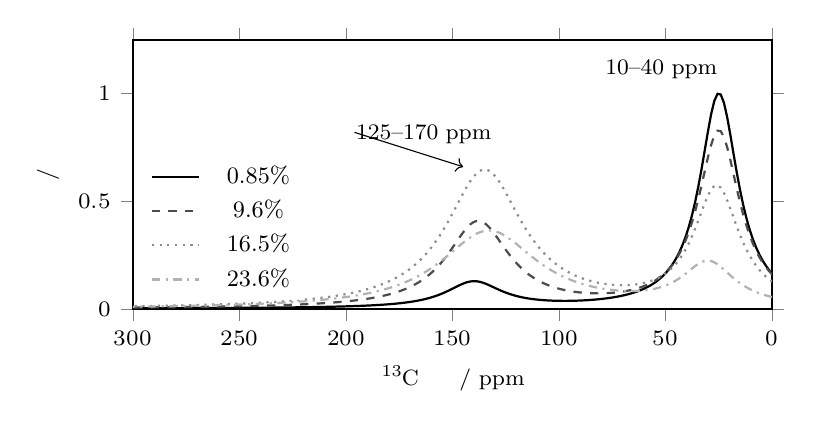
\begin{tikzpicture}
% declare function 必须放在 \begin{tikzpicture} 之后、\begin{axis} 之前，用 \tikzset 声明；
% 线型用有界洛伦兹 1/(1+((x-a)/w)^2)，避免小 w 的高斯指数触发 Dimension too large。
\tikzset{declare function={
  pk(\x,\a,\b) = 1/(1+((\x-\a)/\b)^2);
  spa(\x) = 1.00*pk(\x,25,11) + 0.12*pk(\x,140,16);
  spb(\x) = 0.82*pk(\x,25,12) + 0.40*pk(\x,138,18);
  spc(\x) = 0.55*pk(\x,26,13) + 0.64*pk(\x,135,22);
  spd(\x) = 0.20*pk(\x,30,15) + 0.36*pk(\x,133,28);
}}
\begin{axis}[
  width=\onecolwidth, height=50mm,
  xmin=0, xmax=300, ymin=0, ymax=1.25,
  x dir=reverse,
  xlabel={\ce{^{13}C} 化学位移 / ppm},
  ylabel={相对强度 / 任意单位},
  xtick distance=50, ytick={0,0.5,1.0},
  tick label style={font={\fontsize{8}{9.6}\selectfont}},
  label style={font={\fontsize{8}{9.6}\selectfont}},
  legend style={at={(0.02,0.03)}, anchor=south west, draw=none,
     fill=white, fill opacity=0.9, text opacity=1,
     font={\fontsize{8}{9.6}\selectfont}, row sep=0.5pt, inner sep=1.5pt},
  every axis plot/.append style={thick, no markers, samples=200, domain=0:300},
]
\addplot[black] {spa(x)};
\addlegendentry{积炭 0.85\%}
\addplot[black!70, dashed] {spb(x)};
\addlegendentry{积炭 9.6\%}
\addplot[black!45, dotted] {spc(x)};
\addlegendentry{积炭 16.5\%}
\addplot[black!30, dashdotted] {spd(x)};
\addlegendentry{积炭 23.6\%}
% 承载文字的 node 一律给 text width，否则最长一行会决定整图宽度。
\node[font={\fontsize{8}{9.6}\selectfont}, text width=16mm, align=center, anchor=south]
  at (axis cs:52,1.02) {脂肪碳\\10--40 ppm};
\draw[->, thin] (axis cs:196,0.82) -- (axis cs:145,0.66);
\node[font={\fontsize{8}{9.6}\selectfont}, text width=20mm, align=left, anchor=west]
  at (axis cs:200,0.84) {芳香碳\\125--170 ppm};
\end{axis}
\end{tikzpicture}
\caption{模型计算的 \ce{^{13}C} MAS NMR 谱随积炭量的变化示意\modelmark。读者应看两件事：右侧脂肪碳峰（10--40 ppm）相对下降，
而左侧芳香碳峰（125--170 ppm）从接近本底长成主峰，说明积炭骨架随积炭量增加而芳构化；同时全谱总强度按可检出比例衰减
（积炭 23.6\% 时只有约 29\% 的积炭可由 NMR 检出）。曲线为洛伦兹线型叠加的模型计算，峰位与半峰宽按本节给出的实验区间设定；
峰高之比的绝对值不代表真实碳量之比（受 CP 效率差异控制）。\figsrc{参数取值参考 S1 §8.6.1，书内 p.555--556 / PDF p.47--48}}
\label{fig:c13-coke-model}
\end{figure}

\begin{table}[htbp]
\centering
\caption{\ce{^{13}C} 化学位移与积炭归属（本节实例）。读者应看两件事：不同类型的碳落在不同位移区间，
而「芳香碳区很宽」本身就是聚合芳烃生成的判据，比单个峰的位置更有信息量。}
\label{tab:c13-assign}
{\srcsize
\begin{tabularx}{\columnwidth}{@{}lX@{}}
\toprule
化学位移 & 归属（实例） \\
\midrule
13.5 / 24.0 / 33.0 ppm & 乙烯在脱水 HZSM-5 上 295 K 吸附生成的直链烷烃聚合物（谱峰很宽，是聚合物的谱线特征） \\
10--40 ppm & HZSM-5 上甲醇转化积炭的脂肪族化合物（分布较宽，支链烷烃多于直链烷烃） \\
13--25 ppm & H 型丝光沸石上分布较窄的脂肪烃 \\
约 150 ppm & 直链与支链烯烃 \\
125--145 ppm & HZSM-5 上的芳香化合物 \\
130--170 ppm & H 型丝光沸石的宽芳香碳区，表明存在聚合芳烃 \\
\bottomrule
\end{tabularx}}
\end{table}

\begin{measure}
\textbf{脉冲与条件}：原位池或密封转子；CP/MAS 配高功率 \ce{^{1}H} 去偶与尽可能高的转速，把旋转边带移出关注区（必要时加 TOSS 抑制边带）。

\textbf{必须记录的量}：峰位（归属）、半峰宽、边带间隔（等于转速）与边带相对强度、以及 CP 谱与直接极化谱的强度比。缺转速记录的谱无法判断哪几个峰是边带。

\textbf{如果目标是碳量而不是「有没有」}：必须另做直接极化（单脉冲）谱，循环延迟按最慢的 \ce{^{13}C} $T_1$ 取（芳构化、石墨化程度高的样品常需数十秒以上），并用已知碳量的标样，或与热重、元素分析结果对照标定。只报 CP 谱的峰面积比，不能给出积炭量。
\end{measure}

\begin{dataflow}
\textbf{（1）孔结构决定积炭类型。} 1982 年 Derouane 等首先用原位 \ce{^{13}C} MAS NMR 确定甲醇转化过程中 HZSM-5 与 H 型丝光沸石上的积炭。HZSM-5 上的积炭是分布较宽的脂肪族化合物（10--40 ppm）、一些芳香化合物（125--145 ppm）以及直链与支链烯烃（约 150 ppm），其中支链烷烃多于直链烷烃；H 型丝光沸石上的积炭是分布较窄的脂肪烃（13--25 ppm），但芳香碳区很宽（130--170 ppm），表明存在聚合芳烃。同样的反应物，在不同孔结构里给出了不同的碳骨架。

\textbf{（2）预处理改变同一分子筛上的积炭。} 乙烯在 HZSM-5 上 295 K 吸附并生成直链烷烃聚合物（13.5、24.0、33.0 ppm），宽谱峰显示聚合物的谱线特征；分子筛吸水后经 573 K 处理，谱峰明显窄化，说明高分子量聚合物已裂解生成直链与支链低碳脂肪烷烃，同时还观察到乙苯共振峰。

\textbf{（3）温度改变积炭走向，铝含量只影响其中一支。} 乙烯在 H 型丝光沸石上原位反应：500 K 以下的低温积炭多为直链与支链烷烃，500 K 以上的高温积炭多为聚合芳烃；低温积炭不受分子筛铝含量影响，高温积炭与铝含量有关。可见积炭类型是温度与酸位密度的函数，只报一个「积炭量」不足以描述样品。

\textbf{（4）可检出比例随积炭量下降，损失有三种机制。} HZSM-5 上甲醇转化：积炭量为 0.85\% 时可检测到所有的积炭；积炭量达到 23.6\% 的最高值时，只有 29\% 的积炭可由 NMR 检测。损失的原因是多方面的：其一，\ce{^{1}H} 的自旋--自旋弛豫时间太短，降低了 \ce{^{1}H}$\rightarrow$\ce{^{13}C} 交叉极化的效率；其二，高积炭量时在分子筛外表面生成导电性的石墨结构，干扰了探头的调谐，降低了 \ce{^{13}C} 检测灵敏度；其三，高积炭量的结构中含有芳环离域电子与缺陷位的顺磁中心，降低了 \ce{^{1}H}$\rightarrow$\ce{^{13}C} 交叉极化效率。能够由 NMR 检测的积炭基本上是在分子筛孔道内的；高含量积炭的分子筛表面物种主要是石墨，因此没有 NMR 信号，而这些石墨堵塞了分子筛表面的孔口，阻碍甲醇在通道内的扩散和产物扩散出孔道，从而使分子筛失活。不同类型分子筛上积炭的 \ce{^{13}C} 信号损失程度也不同。

\textbf{（5）结论的正确表述。} \ce{^{13}C} NMR 提供的信息基本上是积炭的化学特征，它取决于分子筛的孔结构、反应物的性质和反应温度；在某些情况下还可以提供积炭中间物的信息。它的局限同样明确：难以得到准确的积炭量数据，只有在轻微积炭或低温积炭的情况下，才可以粗略估计积炭量并确定积炭性质，而且不能区分分子筛孔道内和外表面积的炭。
\end{dataflow}

\begin{pitfall}
\textbf{（1）CP 谱不能直接定量。} 不同类型碳的交叉极化效果不同，\ce{^{13}C} CP/MAS NMR 谱无法用于定量确定积炭量。要把「脂肪碳峰下降、芳香碳峰上升」读成「脂肪碳减少、芳香碳增加」，必须假定各组分的 CP 效率不变；当积炭本身改变了弛豫与顺磁环境时，这个假定并不成立。定量结论应来自直接极化谱，或来自热重、元素分析等独立方法。

\textbf{（2）旋转边带会被误当成真实碳物种。} 边带以转速为间隔出现在真实峰两侧，强度随转速与 CP 条件改变，位置随转速移动；真实碳物种的峰位不随转速移动。再现聚合芳烃、烯碳这类「新物种」之前，先用两个转速对照排除边带。

\textbf{（3）「NMR 不可见」不等于「没有积炭」。} 高积炭量时外表面石墨与顺磁中心使信号消失，可检出量只是积炭的一个子集。特别要注意：23.6\% 积炭只有 29\% 可检出，但本书明确指出可检出的积炭基本位于孔道内，说明「看不见」的那部分并不都等于外表面石墨，其中一部分是孔道内碳因 CP 效率下降而丢失的信号；把差额直接当作外表面积炭会高估石墨量。

\textbf{（4）探头调谐变化属于仪器层面。} 导电石墨改变探头调谐，从而改变灵敏度；跨样品比较峰强前必须重新调谐，并记录调谐与接收增益条件，否则测到的「积炭效应」里混有仪器效应。
\end{pitfall}

\subsubsection{\ce{^{29}Si} MAS NMR 与 \ce{^{27}Al} MAS NMR 研究分子筛积炭}
\src{S1 §8.6.2，书内 p.556--558 / PDF p.48--50}

填充了孔道的积炭影响骨架 \ce{^{29}Si} 和 \ce{^{27}Al} 核的周围环境，使它们的 MAS NMR 谱发生变化，因此这两种技术可用来研究积炭，提供的是\textbf{积炭对分子筛骨架的影响}，而不是积炭本身的化学信息。

\paragraph{（1）\ce{^{29}Si} MAS NMR：骨架弛豫的变化与 H/C}

\begin{principle}
\ce{^{29}Si} 自旋 $I=1/2$，化学位移由骨架硅的 Q$^n$ 环境（铝邻居数）决定，因此谱形本身就是骨架连通性的读数。积炭对它的影响有两条彼此独立的通道：一是孔道内物种改变骨架硅周围的磁环境，使峰位与峰形变化；二是积炭取代了孔道中的顺磁性氧，降低了 \ce{^{29}Si} 和 \ce{^{1}H} 的自旋--晶格弛豫速率，增大了 Si 的自旋--晶格弛豫时间 $T_1$，于是在一定的脉冲循环时间（如 \qty{10}{s}）内磁化矢量不能充分弛豫，从而降低了信号强度。第二条通道提醒我们：信号下降未必是硅少了。

\ce{^{1}H}$\rightarrow$\ce{^{29}Si} 交叉极化（\ce{^{29}Si} CP/MAS NMR）信号的增强与吸附物中氢的含量有关，这一结果可以扩展到积炭研究：CP 信号强度对应于每个晶胞中含氢原子的数目，与积炭量（碳的数目）相比即可得到 H/C 值：
\[
\frac{\mathrm{H}}{\mathrm{C}}=\frac{N_{\mathrm{H}}}{N_{\mathrm{C}}}
\]
其中 $N_{\mathrm{H}}$ 为每个晶胞中的氢原子数（由 \ce{^{29}Si} CP 信号强度标定），$N_{\mathrm{C}}$ 为同一晶胞中积炭碳原子数（由积炭质量分数与晶胞组成换算）。
\tocheck{未对照原页面图像：H/C 的换算式、所用晶胞组成与标定参考样品原书未给出，此处按定义重建；\ce{^{29}Si} 天然丰度与化学位移范围亦未在 §8.6.2 重复给出}
\end{principle}

\begin{dataflow}
\textbf{（1）谱形的变化有阈值。} HZSM-5 分子筛积炭前后的 \ce{^{29}Si} MAS NMR 谱（图 8-17）显示：积炭在 10\%（质量分数）以下时 \ce{^{29}Si} 谱变化不大；积炭到 16.5\% 和 23.6\% 时，谱峰移向低场，峰形发生扭曲并且谱线增宽，半峰宽由 \qty{143}{Hz} 增加到 \qty{218}{Hz}，峰形及位置类似含四丙基胺模板剂的 ZSM-5 分子筛（TPA-ZSM-5）的 \ce{^{29}Si} 谱。

\textbf{（2）CP 强度的线性区。} 积炭量由 0.85\% 变化到 9.6\% 时，\ce{^{29}Si} CP/MAS NMR 信号强度与积炭量呈线性关系；而积炭量为 23.6\% 时，\ce{^{29}Si} CP 信号强度只是积炭 9.6\% 时的一半，原因是高积炭分子筛表面上生成大量石墨，\ce{^{1}H} 数目减少，降低了 \ce{^{1}H}$\rightarrow$\ce{^{29}Si} 交叉极化效率。

\textbf{（3）H/C 值随积炭量下降。} 在 HZSM-5 上测得：积炭量 0.8\% 时 H/C 为 0.9；积炭量 9.6\% 时 H/C 为 0.5；积炭量 23.6\% 时 H/C 为 0.1。氢碳比从接近 1 降到 0.1，与 \ce{^{13}C} 谱上芳构化的图像一致，说明积炭在高积炭量时已高度脱氢。
\end{dataflow}

\paragraph{（2）\ce{^{27}Al} MAS NMR：脱铝、对称性与「NMR 不可见」的铝}

\begin{principle}
\ce{^{27}Al} 自旋 $I=5/2$，是四极核，谱线主要由四极相互作用控制：一阶四极作用由 MAS 消除，中心跃迁剩下的二阶增宽不能由 MAS 消除，其线宽近似随 $\Delta\nu_{1/2}\propto C_Q^{2}/\nu_0$ 变化，其中 $C_Q=e^{2}qQ/h$ 为四极偶合常数，$\nu_0$ 为共振频率。谱线还受自旋--自旋弛豫限制，$\Delta\nu_{1/2}\approx 1/(\pi T_2)$。积炭后谱的变化是这两种增宽机制共同作用的结果：积炭分子取代了分子筛中的水使水含量减少，而且使 Brönsted 酸位上的 H$^{+}$ 在铝核周围停留更长的时间，从而改变了铝核周围的电场梯度，引起四极相互作用的加强和位移；随着 \ce{^{27}Al} 峰宽的增加，骨架 \ce{^{27}Al} 化学位移向高场移动。积炭后 \ce{^{27}Al} 谱的变化与吸附烷烃和催化剂脱水效应很类似。
\tocheck{未对照原页面图像：二阶四极增宽与线宽的表达式按标准形式补入（原书以文字描述），是否含 $(1+\eta^{2}/3)$ 因子及具体系数需核对原页}

\textbf{从谱变化到失活类型的推断链。} 积炭量增大时，积炭分子覆盖了分子筛的 Brönsted 酸位，改变了骨架铝的对称性且增大了 \ce{^{27}Al} 的四极偶合常数；四极偶合常数越大，\ce{^{27}Al} 信号越弱，NMR 可观察到的铝核越少。这种情况下，催化剂失活主要是由 Brönsted 酸位中毒引起的。
\end{principle}

\begin{measure}
\ce{^{29}Si}：循环延迟要按测得的 $T_1$ 设定（本书实例用 \qty{10}{s}），比较积炭前后强度前先确认样品 $T_1$ 是否改变；CP/MAS 需注明接触时间，并用直接极化谱作参照。

\ce{^{27}Al}：四极核建议用高场、小扳转角（短而强的脉冲）与尽可能高的转速，以减小二阶四极增宽与边带；必须报转速、脉冲条件与参考物（骨架四配位铝约 60 ppm、非骨架铝约 0 ppm、畸变晶格铝约 30 ppm 的归属都建立在同一参考标度上）。不同磁场、不同转速下测得的峰强与峰宽\textbf{不可}直接比较。
\end{measure}

\begin{dataflow}
\textbf{（1）三条曲线的走向。} 积炭量对骨架 \ce{^{27}Al} 信号强度（a）、峰宽（b）和化学位移（c）的影响（图 8-18）规律一致：随积炭量增加，骨架 \ce{^{27}Al} 峰强度降低、峰宽增加、化学位移向高场移动。

\textbf{（2）非骨架铝参与积炭。} 图 8-19 是脱铝 HZSM-5 分子筛上丙酮转化期间的 \ce{^{27}Al} MAS NMR 谱。初始样品出现两个共振信号：60 ppm 的 A 信号为四配位骨架 Al，0 ppm 的 R 信号为非骨架 Al。积炭量为 10.7\% 时，A 峰变宽，非骨架铝峰变成一个肩峰；把催化剂部分氧化使积炭量降为 5.5\% 时，A 峰重新窄化，非骨架铝峰重新出现，只是强度比初始状态低。这种现象说明在 HZSM-5 分子筛上，非骨架铝物种参与了积炭的生成，而且这一过程在部分氧化后可以部分逆转。
\tocheck{未对照原页面图像：图 8-19 的峰标签在 OCR 中前后不一致（先记为 A、R，随后又出现 B），此处按正文归属写作 A（骨架铝 60 ppm）与非骨架铝峰（0 ppm）}

\textbf{（3）骨架铝也会被卷进去。} 在脱铝的 HY 分子筛上，正己烷裂解积炭样品的 \ce{^{27}Al} MAS NMR 谱中，除了骨架铝和非骨架铝信号外，还出现了一个 30 ppm 共振峰，归属为易变形和易碎的晶格铝；随积炭量增加，该峰强度增加，说明积炭后引起某些骨架铝破碎，形成了 30 ppm 铝物种。因此在相当高积炭量的分子筛中，一些骨架铝也卷入了积炭的生成。

\textbf{（4）两种核合起来能给出什么。} 综合分析 \ce{^{29}Si} 和 \ce{^{27}Al} MAS NMR 实验结果，可以研究积炭对分子筛的影响、积炭后分子筛的脱水（及相应的骨架环境变化）和积炭占有的体积；结合催化活性的测量，进而得到酸位中毒或孔道堵塞的催化剂失活信息。
\tocheck{未对照原页面图像：原文「积炭后分子筛脱氧和脱水量」中的「脱氧」含义存疑（疑为 OCR 或原书表述），此处按脱水与体积占据理解}
\end{dataflow}

\begin{pitfall}
\textbf{（1）\ce{^{27}Al} 无信号，不等于没有铝物种。} 四极增宽使部分铝核「NMR 不可见」：积炭覆盖 B 酸位后四极偶合常数增大，\ce{^{27}Al} 信号变弱，可观察到的铝核变少。把「谱上没有这个峰」直接读成「样品里没有这种铝」，是本节最容易犯的错。提高磁场有助于观察，但不同磁场下的强度不可相互换算。

\textbf{（2）\ce{^{27}Al} 强度下降不等于脱铝量。} 强度同时受 $C_Q$ 与 $T_2$ 影响，要判断是否真的脱铝，需与 \ce{^{29}Si} 的 Q$^n$ 分布或化学分析（如 ICP）对照。

\textbf{（3）30 ppm 峰不能直接当作「新的骨架铝物种」的浓度。} 它的归属是易变形、易碎的晶格铝，其强度依赖线型分解的可靠性；在只有一条宽包络时，把它分出来本身就带主观性。

\textbf{（4）\ce{^{29}Si} 信号下降不等于骨架硅减少。} 积炭使 Si 的 $T_1$ 变长，循环时间不足就会造成「假损失」；比较积炭前后必须先测 $T_1$ 或统一使用足够长的循环延迟。同理，\ce{^{29}Si} CP 谱的强度受 \ce{^{1}H} 数目控制，在高积炭量时失效（23.6\% 时只有 9.6\% 时的一半）。
\end{pitfall}

\begin{crosscheck}
\ce{^{29}Si} 与 \ce{^{27}Al} 是一对骨架报告者，但两者都可能因非化学原因变弱（前者因 $T_1$ 变长，后者因 $C_Q$ 增大）。因此「骨架损伤」的结论至少要与 \ce{^{1}H} 的 B 酸位计数、催化活性测量三方对照：单靠 \ce{^{27}Al} 强度下降，既可能是脱铝，也可能是四极增宽把铝藏了起来；而孔道的几何后果（窗口是否堵死、笼是否缩小）由 \ce{^{129}Xe} 回答（§8.6.4）。
\end{crosscheck}

\subsubsection{\ce{^{1}H} MAS NMR 研究分子筛积炭}
\src{S1 §8.6.3，书内 p.559--560 / PDF p.51--52}

\ce{^{1}H} MAS NMR 也是研究分子筛积炭的有效方法：它可以提供积炭后分子筛中仍有活性的 Brönsted 酸位信息。通过脉冲场梯度的自扩散测量可以确定积炭的位置和孔内与外表面扩散的变化；当已知积炭量时，可通过 \ce{^{1}H} MAS NMR 谱确定 H/C 值，进而确定分子筛晶体孔道内和外表面上积炭化合物的性质；对分子筛中吸附分子进行 \ce{^{1}H} 自旋--晶格和自旋--自旋弛豫时间 $T_1$、$T_2$ 的测量，可以得到积炭分子在分子筛孔道中的分布信息。

\begin{measure}
\textbf{转速是前提}：\ce{^{1}H} 同核偶极增宽很大，转速不足时 2.0 ppm 的 Si--OH 峰与 4.2 ppm 的 B 酸峰无法分辨。必须报转速。

\textbf{定量}：单脉冲谱，循环延迟取 $5T_1$ 以上（或先用反转恢复／饱和恢复测 $T_1$）；\ce{^{1}H} 的背景（探头、空转子、吸附水）要单独采集并扣除。峰位归属：2.0 ppm 为 Si--OH，4.2 ppm 为 B 酸中心。

\textbf{弛豫与自扩散}：$T_1$ 用反转恢复或饱和恢复；$T_2$ 用回波序列测量（固体中直接读 FID 衰减会低估 $T_2$）；脉冲场梯度（PFG）\ce{^{1}H} NMR 给出孔内与晶间的自扩散系数，用于判断积炭位置与扩散通道的变化。
\end{measure}

\begin{dataflow}
\textbf{（1）两种探针分子给出两种位置信息。} Lechert 等研究了不同脱铝程度的 HY 分子筛在 530 K 丁烯转化过程中的积炭情况，比较分子筛积炭前后吸附正丁烷和苯的能力及 \ce{^{1}H} 的 $T_1$、$T_2$ 弛豫时间。与积炭前样品相比，积炭后分子筛吸附正丁烷的能力降低不大，但 \ce{^{1}H} 的 $T_1$ 和 $T_2$ 值减小，表明吸附的正丁烷分子的重新取向运动受到很大阻碍，积炭附近分子的堆积发生了变化。吸附苯的情况恰恰相反：\ce{^{1}H} 的 $T_1$ 和 $T_2$ 值变化不大，表明积炭对苯分子的运动影响很小，但吸附能力却大大降低。

\textbf{（2）观察与推断要分开写。} 观察：吸苯量大幅下降，而苯的 $T_1$、$T_2$ 几乎不变。推断：苯分子主要位于分子筛孔道之间的窗口，分子绕着它们的二重轴运动，同时伴随着相邻位之间的跳跃。这一推断解释了「进不去但动得动」的组合，也说明吸附量的变化与弛豫的变化必须分别解读：吸正丁烷是「动不了但进得去」，吸苯是「进不去但动得了」。

\textbf{（3）B 酸位的存活数量。} Ernst 等研究了 HZSM-5 分子筛积炭前后的 \ce{^{1}H} MAS NMR 谱：2.0 ppm 是 Si--OH 峰，4.2 ppm 是 B 酸中心；积炭前 B 酸相对含量很大，积炭后 B 酸的峰强降低，而 Si--OH 含量大大增加，并且出现一个很大的宽峰，这是由积炭分子、或由酸羟基与积炭分子强偶极相互作用所致。根据 B 酸峰强度的降低可以计算出积炭后仍存在的活性 B 酸位的数量；参考 \ce{^{27}Al} MAS NMR 谱中骨架铝积炭后的变化，可分析出积炭使 B 酸位发生了中毒。

\textbf{（4）这一节的出口。} \ce{^{1}H} MAS NMR 谱主要用于估算 B 酸位的数量，结合 \ce{^{27}Al} MAS NMR 谱等确定积炭引起分子筛失活的类型；测量吸附探针分子的弛豫时间和脉冲梯度 \ce{^{1}H} NMR 谱可以提供积炭在分子筛晶体孔道中的分布信息；当已知积炭量时，\ce{^{1}H} MAS NMR 谱可以测量积炭前后的 H/C 值，但要注意：\ce{^{1}H} MAS NMR 谱测出的 H/C 值是含孔道内和外表面全部积炭的数值。
\end{dataflow}

\begin{pitfall}
\textbf{（1）两个 H/C 的口径不同。} 由 \ce{^{29}Si} CP 强度所得的 H/C 只在 CP 强度与积炭量成线性的区间可靠（本例为 0.85\%--9.6\%），高积炭时表面石墨使 \ce{^{1}H} 减少而系统性偏低；由 \ce{^{1}H} MAS NMR 谱所得的 H/C 包含孔道内与外表面的全部积炭。报 H/C 时必须同时说明口径与积炭量区间，两个数值不一致并不矛盾。

\textbf{（2）宽峰不是新酸位。} 积炭后出现的很大宽峰可由积炭分子或酸羟基与积炭分子的强偶极相互作用造成，属于相互作用导致的增宽；把它当成「新增的酸性物种」会同时高估酸位数量。

\textbf{（3）分峰不当会双向失真。} 该宽峰与 4.2 ppm 的 B 酸峰叠加，分峰不当会同时抬高「剩余 B 酸」与「新增物种」；报剩余 B 酸比例时应给出分峰模型与误差。

\textbf{（4）背景水与 Si--OH 重叠。} 2.0 ppm 附近的 Si--OH 与探头／吸附水的 \ce{^{1}H} 背景重叠，判断「Si--OH 大大增加」之前必须扣背景，否则会把水的变化读成羟基的变化。
\end{pitfall}

\begin{crosscheck}
\ce{^{1}H} 给出的是「还剩多少 B 酸位」，\ce{^{27}Al} 给出的是「骨架铝变成了什么」。只有两者对照，才能把 B 酸峰的降低归因于积炭覆盖／中毒，而不是骨架脱铝本身；再叠加活性数据，才能把「酸位中毒」与「孔道堵塞」两种失活类型分开。
\end{crosscheck}

\subsubsection{吸附氙的 \ce{^{129}Xe} NMR 研究分子筛积炭}
\src{S1 §8.6.4，书内 p.560--562 / PDF p.52--54}

测定不同分子筛在不同反应条件下积炭后的吸附氙 $\delta=f(n)$ 曲线，可获得分子筛结构和反应物性质对积炭影响的信息，确定积炭性质和积炭后分子筛结构的变化。Xe 是惰性原子，不参与反应、不改变酸性，它的化学位移由所处空间的尺寸与碰撞环境决定，因此对孔道尺寸与堵塞极其敏感。在积炭研究中，它是少数能直接反映\textbf{孔道空间占据}几何的探针：\ce{^{13}C} 告诉你积炭是什么，\ce{^{129}Xe} 告诉你孔道被占成了什么形状。

\begin{principle}
在快速交换极限下，测得的 \ce{^{129}Xe} 化学位移与 Xe 吸附量 $n$ 的关系可写成线性形式
\[
\delta(n)=\delta_{n\to 0}+k\,n
\]
其中 $\delta_{n\to 0}$ 是外推到零氙吸附量时的位移，反映 Xe 与孔壁及强吸附位（例如非骨架铝）的相互作用，以及在孔口受阻时扩散受限的程度；斜率 $k$ 反映 Xe--Xe 碰撞的频率，与 Xe 可自由活动的体积成反比。由此得到三条判读规则：

（1）两曲线平行（$k$ 相同）而 $\delta_{n\to 0}$ 增大：自由体积基本不变，但 Xe 在笼间的扩散受阻，积炭主要落在窗口（笼与笼之间的通道）上。

（2）$k$ 与 $\delta_{n\to 0}$ 同时增大：自由体积本身下降，且有部分积炭位于晶体外表面，阻碍 Xe 进入。

（3）由积炭与未积炭样品的斜率之比，可以估算可吸附 Xe 的体积下降幅度：
\[
\frac{V_{\text{积炭样品}}}{V_{\text{未积炭样品}}}\approx\frac{k_{\text{未积炭样品}}}{k_{\text{积炭样品}}}
\]
本节实例给出：丙烯裂解生成 15\% 与 33\% 积炭时，可吸附 Xe 的体积分别降低 52\% 与 90\%。

要记住两条轴的物理含义：\textbf{斜率的变化说明自由体积变了，斜率不变而截距变化说明扩散或强吸附位变了}。例如 15\% 积炭样品的斜率与 10.5\% 积炭样品相同，说明此时积炭主要影响晶孔的外表面。
\tocheck{未对照原页面图像：$\delta=f(n)$ 的线性表达、斜率比与可吸附体积下降的换算式（是否取倒数、是否需要独立的 Xe--Xe 参考位移标定）原书只给结果未给公式，此处按常用形式重建}
\tocheck{未对照原页面图像：\ce{^{129}Xe} 天然丰度与「Xe 原子的动态直径约 0.44 nm」为按标准值补入，原书 §8.6.4 只写「减少到约为 Xe 原子的动态直径」而未给数值}
\end{principle}

\begin{measure}
\textbf{样品}：密封管／转子中定量引入 Xe（由压力与体积标定吸附量 $n$），并等待吸附平衡；同一批样品必须做未积炭参照曲线。

\textbf{变温是必需项}：本节的判读大量依赖「斜率与 $\delta_{n\to 0}$ 是否随温度变化」，因此必须做温度序列；只测一条等温曲线，无法区分「自由体积下降」与「扩散受阻」。

\textbf{参考与延迟}：以氙气共振峰为 0 ppm（本节实例中 0 ppm 峰即氙气峰）；\ce{^{129}Xe} 的 $T_1$ 较长，循环延迟要足够。Xe 化学位移跨度大，对磁场要求不高，但对 Xe 量的标定要求高；比较时用斜率与截距，而不是某个单压力点的位移值。
\end{measure}

\begin{dataflow}
\textbf{（1）窗口堵塞的判据。} 1988 年 Ito 等首先将 \ce{^{129}Xe} NMR 用于正己烷及丙烯裂化的 HY 分子筛积炭研究。正己烷为反应物时，未积炭样品（HY）与积炭量 5.5\%（He-5）的 $\delta=f(n)$ 曲线互相平行，说明二者斜率相同，但 $\delta_{n\to 0}$ 值不同；He-5 的 $\delta_{n\to 0}$ 增大，表明氙在超笼间的扩散减少，积炭位于超笼之间的窗口上。

\textbf{（2）自由体积下降与外表面堵塞。} 丙烯为反应物、积炭分别为 15\%（Pr-15）和 33\%（Pr-33）时，与未积炭样品相比，$\delta=f(n)$ 直线的斜率及 $\delta_{n\to 0}$ 均增加很大；根据积炭和未积炭样品斜率之比，可计算出积炭 15\% 和 33\% 的分子筛可吸附 Xe 的体积分别降低 52\% 和 90\%。这表明积炭后不仅分子筛孔体积大大降低，而且部分积炭位于晶体的外表面，阻碍 Xe 进入超笼。33\% 积炭样品的 \ce{^{129}Xe} 谱出现两个峰：一个是很宽且低场位移很大的谱峰（157 ppm），为吸附在与积炭相连的超笼中的 \ce{^{129}Xe}；另一峰出现在 10 ppm，与 Xe 压力无关，是吸附在分子筛孔道内积炭形成的中孔或微笼中的 \ce{^{129}Xe}。这些结果直接显示了积炭的位置。

\textbf{（3）初始积炭落在非骨架铝附近。} Barrage 等系统研究了庚烷裂解时失活的 HY 分子筛中积炭的分布。未积炭样品的 $\delta=f(n)$ 曲线在低 Xe 浓度时出现一个最低点，并且随温度升高 $\delta_{n\to 0}$ 增大，这是 Xe 与非骨架铝的强吸附位相互作用的特征，\ce{^{27}Al} NMR 谱也证明了这一点。当积炭量为 3\%、10.5\% 和 15\% 时，$\delta=f(n)$ 曲线全部变成直线，这表明最初始的积炭位于或接近于非骨架 Al 物种，积炭阻碍了非骨架 Al 物种与 Xe 原子的相互作用，消除了曲线中的最低点。而且，当积炭量达到 3\% 时，庚烷裂解的活性丧失一半多，这说明非骨架 Al 物种在反应初始对 HY 分子筛裂解活性起主导作用。

\textbf{（4）积炭由非均匀走向均匀的三段图像。}
低积炭量（3\%）：斜率变化较小、与初始样品相近，自由体积几乎不受影响，但 $\delta_{n\to 0}$ 增加了，且两者随温度升高而发生变化，说明 Xe 的扩散受阻，积炭初始是非均匀的并且主要沉积在超笼的窗口上。
中等积炭量（10\%）：$\delta=f(n)$ 曲线的斜率和 $\delta_{n\to 0}$ 都增加，但与吸附温度无关，此时积炭的生成更均匀，且超笼内也生成积炭，将其直径减少到约为 Xe 原子的动态直径；温度升高时 Xe 原子扩散未受到阻碍，所以斜率增加，而 $\delta=f(n)$ 曲线与温度无关。
高积炭量（15\%）：\ce{^{129}Xe} 谱出现三条谱线，低场的一条宽峰，其化学位移值随 Xe 浓度呈线性变化；第二条谱线出现在 44 ppm，与 Xe 压力无关；0 ppm 峰是氙气的共振峰。三条谱线说明 Xe 吸附在不同的位置上，相互之间在 NMR 时域内没有交换。其 $\delta=f(n)$ 曲线斜率与 10.5\% 积炭量的样品相同，但 $\delta$ 值增加很大，表明 Xe 的平均自由通道很小、扩散严重受阻、许多笼被积炭堵塞：积炭不仅大大减小了内部自由体积，而且在分子筛晶孔之间形成了微孔或中孔；斜率相同表明积炭主要影响晶孔的外表面。

\textbf{（5）可推广性。} 以同样的方法，人们对 HZSM-5 分子筛的积炭也进行了大量研究，确定了不同积炭量时积炭的分布。总之，分子筛吸附 Xe 后测定 \ce{^{129}Xe} NMR 的 $\delta=f(n)$ 曲线，可以直接得到内部积炭位置及积炭量信息，能够显示分子筛结构和反应物性质对积炭和再生的影响。
\end{dataflow}

\begin{pitfall}
\textbf{（1）多条谱线不等于多种积炭物种。} 33\% 样品的两个峰（157 ppm 的宽峰、10 ppm 且与压力无关的峰）与 15\% 样品的三条谱线（低场宽峰、44 ppm、0 ppm），说明的是 Xe 处于不同位置且在 NMR 时域内互不交换。其中 0 ppm 峰是氙气本身，不能计入孔内物种；「与压力无关」是判断该峰来自封闭小空间（中孔、微笼）的关键证据。

\textbf{（2）位移变化的来源不止「孔变小」。} 非骨架铝的强吸附位与温度都会改变 $\delta$ 与曲线形状。未积炭样品的曲线最低点消失，是积炭覆盖了强吸附位，而不是孔容恢复；不做未积炭对照、不做变温，很容易把这一现象误读为「积炭改善了孔道」。

\textbf{（3）温度依赖性是判据而不是噪声。} 斜率是否随温度变化、$\delta_{n\to 0}$ 是否随温度变化，分别对应自由体积与扩散受阻；两者必须分别报告，否则 3\% 与 10\% 这两段图像无法区分。

\textbf{（4）Xe 进不去的孔，测不到。} 探针法的固有边界：被完全堵死的空间不产生 \ce{^{129}Xe} 信号，所以 \ce{^{129}Xe} 不会「报告」那部分孔容损失；把斜率比换算成体积下降，也依赖一个独立的体积标定。
\end{pitfall}

\begin{crosscheck}
\textbf{（1）与氮吸附孔容下降的互补关系。} 77 K 氮吸附给出的是孔容／比表面积的总量下降，是一个标量：它能告诉你「少了多少」，但不告诉你积炭落在窗口、笼内还是外表面。\ce{^{129}Xe} 的 $\delta=f(n)$ 恰好补上「位置」这一维：曲线平行而截距升高对应窗口堵塞；斜率与截距同时升高对应笼内自由体积下降并伴以外表面堵塞；出现与压力无关的新峰对应积炭内部新生成了微孔或中孔；$\delta_{n\to 0}$ 的温度依赖对应扩散是否受阻。反过来，\ce{^{129}Xe} 只能报告 Xe 能到达的空间，完全堵死的孔不产生信号，因此「孔容一共降了多少」仍需氮吸附这类总量方法提供基准，而把斜率之比换算成体积下降也依赖独立标定。两者的关系可以一句话概括：\textbf{氮吸附给总量（多少），\ce{^{129}Xe} 给分布（在哪、以什么方式堵）}，二者不可互相替代。（原书 §8.6.4 未与氮吸附数据对照，这一互补关系是按方法学写出的推论。）

\textbf{（2）与其余三种核的合围。} \ce{^{13}C} 给积炭的化学身份，\ce{^{1}H} 给剩余 B 酸位与 H/C，\ce{^{29}Si}／\ce{^{27}Al} 给骨架损伤，\ce{^{129}Xe} 给孔道几何。本节中一个可用的联动判据是：积炭只有 3\% 时裂解活性已丧失一半多，而自由体积几乎不受影响（斜率与初始样品相近），这是典型的酸位中毒而不是孔道堵塞，与 \ce{^{27}Al} 谱中非骨架铝强吸附位被积炭覆盖的观察一致。
\end{crosscheck}

\begin{methodsum}
积炭的四问与四种核的对应关系可以压缩成一句话：\textbf{\ce{^{13}C} 回答「是什么」，\ce{^{29}Si}／\ce{^{27}Al} 回答「骨架被弄坏到什么程度」，\ce{^{1}H} 回答「还剩多少酸位、氢在谁身上」，\ce{^{129}Xe} 回答「堵在哪里、堵成什么样」。}

组合使用有三条纪律：（1）凡涉及「量」的数字，必须说明是直接极化还是 CP、有无独立标定；（2）凡涉及「消失」的结论，必须先排除弛豫变慢、四极增宽、旋转边带与探头调谐等非化学原因；（3）凡涉及「位置」的结论，至少要有两个独立方法支持（例如窗口堵塞同时由 \ce{^{129}Xe} 的截距升高与 \ce{^{1}H} 上 B 酸位存活数佐证）。
\end{methodsum}

\begin{table}[tbp]
\centering
\caption{四种核在分子筛积炭研究中的分工对照。读者应把同一行的四项一起读：「测什么」决定它能回答哪个问题，
「定量前提」决定数字能不能当量用，「主要干扰」决定结论的边界；只取信号强度、不看后两列，是本领域最常见的误用。}
\label{tab:nuclei-coke}
{\srcsize
\begin{tabularx}{\twocolwidth}{@{}p{13mm}p{27mm}p{45mm}p{38mm}X@{}}
\toprule
核种 & 测什么 & 能给出的积炭信息 & 定量前提 & 主要干扰 \\
\midrule
\ce{^{13}C} & 碳的化学环境（0--300 ppm） &
脂肪碳 10--40 ppm、烯碳约 150 ppm、芳香碳 125--145 ppm、聚芳烃宽芳香区 130--170 ppm；随分子筛、反应物与温度改变 &
CP 谱不能定量；若报碳量需直接极化谱 + 足够长循环延迟 + 已知标样（或热重／元素分析） &
各类型碳 CP 效率不同；旋转边带伪装成物种；高积炭时导电石墨与顺磁中心使信号丢失（23.6\% 积炭仅 29\% 可检出） \\
\ce{^{29}Si} & 骨架硅的 Q$^n$ 环境与 $T_1$ &
积炭对骨架的扰动：峰移向低场、半峰宽 \qty{143}{Hz} 增至 \qty{218}{Hz}、信号下降；CP 强度给出 H/C（0.8\%、9.6\%、23.6\% 积炭时为 0.9、0.5、0.1） &
CP 强度按每晶胞含氢数标定；H/C 需同时知道积炭量；只在 CP 强度与积炭量成线性的区间（0.85\%--9.6\%）可靠 &
积炭取代孔道中顺磁性氧使 Si 的 $T_1$ 变长，循环时间不足即出现「假损失」；表面石墨减少 \ce{^{1}H} 使 CP 效率下降 \\
\ce{^{27}Al} & 骨架四配位 Al（约 60 ppm）、非骨架 Al（约 0 ppm）、畸变晶格 Al（约 30 ppm） &
脱铝与骨架损伤；积炭覆盖 B 酸位使骨架铝对称性下降、四极偶合常数增大；非骨架铝与部分骨架铝参与积炭生成 &
需同磁场、同转速、同脉冲条件下比较；峰强同时受 $C_Q$ 与 $T_2$ 影响，不能直接换算成铝量或脱铝量 &
四极增宽使部分铝「NMR 不可见」，无信号不等于无物种；强度下降未必是脱铝；30 ppm 峰依赖线型分解 \\
\ce{^{1}H} & Si--OH（约 2.0 ppm）、B 酸中心（约 4.2 ppm）；探针分子的 $T_1$、$T_2$ 与自扩散 &
积炭后仍存活的 B 酸位数量（据此判断酸位中毒）；H/C 值；积炭在孔道内与外表面的分布（弛豫 + 脉冲场梯度自扩散） &
需已知积炭量；B 酸定量需与 \ce{^{27}Al} 对照，并用 $5T_1$ 以上循环延迟、扣除探头与水背景 &
探头／水背景与 Si--OH 峰重叠；积炭宽峰与 B 酸峰的强偶极重叠使分峰失真；所得 H/C 含内、外表面全部积炭 \\
\ce{^{129}Xe} & 化学位移与 Xe 吸附量的关系 $\delta=f(n)$（斜率与 $\delta_{n\to 0}$） &
积炭位置（超笼窗口／笼内／外表面）；可吸附 Xe 体积下降（15\%、33\% 积炭分别降 52\%、90\%）；谱峰数目给出互不交换的 Xe 环境（如 157 ppm、10 ppm、44 ppm） &
需与未积炭样品比较斜率与截距；变温测量是把「自由体积下降」与「扩散受阻」分开的前提；Xe 量须定量标定 &
温度与强吸附位（非骨架 Al）同样改变 $\delta$；多峰不等于多物种（0 ppm 为氙气）；Xe 进不去的孔完全测不到 \\
\bottomrule
\end{tabularx}}
\end{table}

\srcnote{本节覆盖 S1 §8.6（书内 p.555--562 / PDF p.47--54）：积炭失活的基本图像与四种核的分工；其中 \ce{^{13}C} 部分见 §8.6.1，\ce{^{29}Si}／\ce{^{27}Al} 部分见 §8.6.2，\ce{^{1}H} 部分见 §8.6.3，\ce{^{129}Xe} 部分见 §8.6.4。}
}{}
\IfFileExists{chapters/parts/ch08-d.tex}{\input{chapters/parts/ch08-d}}{}
\IfFileExists{chapters/parts/ch08-e.tex}{\input{chapters/parts/ch08-e}}{}
}{}
\IfFileExists{chapters/ch09.tex}{% chapters/ch09.tex —— 第 9 章 表面分析技术基础
% 装配层：只负责按顺序引入各分片。分片缺失时跳过，便于增量成书。
% 分片文件：chapters/parts/ch09-{a..e}.tex

\IfFileExists{chapters/parts/ch09-a.tex}{\chapterstart{表面分析技术基础}%
{本章导读：表面分析的共同前提是「信号必须在表面产生、并能量无损地逃出来」，所以先要回答的不是
「用哪台谱仪」，而是「信号来自多深、这个表面能保持多久」。本章讲表面的定义、表面与体相的差别、
信息深度与超高真空的关系（9.1），再以 X 射线光电子能谱（XPS）为样本讲清基本原理、仪器组成与
实验方式（9.2）。XPS 的定量、分峰与化学态判读，以及 AES、UPS、SIMS 等方法的选择，留待后续分片。}
\label{ch:09}

% ================================================================
%  第 9 章 表面分析技术基础（分片 a）
%  源：S2（下册）第 9 章，书内 p.567—614 / PDF p.59—106
%  覆盖：9.1 关于表面；9.2.1 历史进程（导航保留）；9.2.2 基本原理；
%        9.2.3 仪器与主要组成部件；9.2.4 实验方式
%  状态：分片 a 完稿；9.2.5 及以后由分片 b/c/d 续写
% ================================================================

\subsection{关于表面}

\begin{probout}
表面分析测量的是固体最外层约 0.5—10 nm 内的\textbf{元素组成、化学态、原子排列与电子结构}。
原始数据只有一条曲线：某类出射粒子（光电子、俄歇电子、二次离子、散射离子）的强度随能量（或
质量）的分布。由此换算出的量有三类：\textbf{元素种类与相对含量}（原子百分比）、\textbf{化学态}
（价态与化学环境），以及它们沿深度与横向的分布。它不直接给出体相组成，也不直接给出催化活性；
含量是相对值，其定量依赖相对灵敏度因子与「采样深度内组成均匀」这一假设。
\end{probout}

\subsubsection{表面的定义与厚度}

两种异态物质之间紧密接触的层称为界面，物体与真空或气体接触的界面称为表面，表面分析着重研究
固体表面，即气-固两相界面（特殊情况下也研究离子液体等特殊液态物质的表面）。表面层通常指一到
两个单层，信息来自零点几纳米到几纳米深处。这个尺度有多小：金属表面 $1$ cm$^{2}$ 的表面层区域
内约有 $10^{15}$ 个原子，而 $1$ cm$^{3}$ 立方体内的原子总数约 $10^{23}$ 个，表面原子只占体相
原子总数的 $10^{-8}$，即 $10^{-6}\%$——用体相灵敏的方法看表面，等于在约一亿个原子里找一个
原子。\tocheck{未对照原页面图像：原 OCR 作「百分数为 106\%」，上标负号丢失；按
$10^{15}/10^{23}=10^{-8}$ 重建。}

\subsubsection{表面与体相的差别}

表面是固体的终端，是晶体三维周期结构与真空之间的过渡区。在动力学与热力学平衡的前提下，表面的
化学组成、原子排列、原子振动状态均有别于体相，原因有两条：① 表面向外一侧没有邻近原子，存在
不饱和化学键即\textbf{悬挂键}，因此化学性质很活泼，极易吸附、氧化与重构；② 固体内部的三维
周期结构在表面中断，表面原子的\textbf{电子状态}（表面态、功函数、振动模式）也有异于体相。
所以表面分析的内容包括表面的形貌、化学组成、原子结构、原子态与电子态——每一项都需要不同的
探测粒子与不同的信息深度，没有一种技术能同时给出全部答案。
\src{S2 §9.1，书内 p.569—570 / PDF p.60—61}

\subsubsection{真实表面的保持：为什么必须超高真空}

在通常的大气环境下，一个新鲜表面很快就被大气组分沾污。\qty{25}{\celsius} 空气中 \ce{N2} 在
表面上形成单层所需的时间随压强急剧变化：$760$ torr 时只需约 $2.9\times10^{-9}$ s，
$10^{-6}$ torr（约 $1.3\times10^{-4}$ Pa）时约 $2.2$ s，$10^{-9}$ torr 时才延长到约
$2.2\times10^{3}$ s。换一种算法：在 $10^{-4}$ Pa、$300$ K 的 \ce{N2} 气氛中，每平方厘米每秒
有 $3.88\times10^{14}$ 个分子撞到表面，而典型固体表面约 $10^{15}$ 原子/cm$^{2}$，所以在
$10^{-4}$ Pa 这种「看起来已经很干净」的真空里，几秒钟就能盖满一个单层。表面被覆盖满一个单层
称为 1 Langmuir（1 L），$1$ L $\approx 10^{-4}$ Pa$\cdot$s，即 $10^{-4}$ Pa 下停留 1 s 就
等于 1 L 的暴露量。

真空区划对表面分析的意义并不相同：低真空（$10^{3}$—$10^{5}$ Pa）与中真空
（$10^{-1}$—$10^{3}$ Pa）下分子平均自由程 $\lambda$ 小于或接近容器直径 $d$，以分子之间的
碰撞为主，只够样品传输与粗处理；高真空（$10^{-6}$—$10^{-1}$ Pa）下 $\lambda>d$，但单层覆盖
时间仍只有秒级，只够快速进样；只有超高真空（$10^{-10}$—$10^{-6}$ Pa）把单层形成时间延长到
$10^{2}$—$10^{6}$ s，才是表面分析的常规工作区（极高真空 $<10^{-10}$ Pa，仅特殊需求使用）。
超高真空起两个作用：使一个较为真实的
表面在相当长的时间（$10^{2}$—$10^{6}$ s）内得以保持，以完成一次真正的表面分析；同时使出射
粒子（主要是电子）尽量少与气体分子碰撞，从而能量无损地到达能量分析器。所以说，没有超高真空
就没有表面科学。推论是：表面分析的每一炉实验都把时间当作消耗品，从清洁完成到录谱结束必须
控制在单层时间以内。\src{S2 §9.1，书内 p.570—571 / PDF p.61—62，表 9-1、表 9-2}

\tocheck{未对照原页面图像：本节 $10$ 的负指数在原 OCR 层普遍丢失上标负号，已按物理含义与
表 9-2 的区划重建，需与书内 p.570—571 原页核对。}

\subsubsection{信息深度：电子逃逸深度与非弹性散射平均自由程}

$1$ keV 量级（XPS 激发源的典型能量）的 X 射线能穿透约 1000 nm 而不显著衰减，而具有同样能量的
电子只能穿透约 10 nm。正是这个差别使 XPS 成为表面灵敏的技术：即使 X 射线在整个穿透深度内都
激发了光电子，也只有最外面约 10 nm 内产生、并且能能量无损地走到表面的电子才携带元素特征信息。
光电子在途中会遇到弹性散射（只改变方向）与非弹性散射（能量也受损失）；一旦发生非弹性碰撞，
电子失去原有的元素特征，成为谱图上抬高的连续本底。因此 XPS 采集到的出射光电子来自深度

\begin{equation}\label{eq:sampling-depth}
d=3\lambda\cos\theta
\end{equation}

式中 $\theta$ 为出射电子与样品面法线的夹角；$\lambda$ 为光电子的非弹性散射平均自由程
（\term{IMFP}{inelastic mean free path}{非弹性散射平均自由程}）。各深度的贡献按
$I(d)/I_{\infty}=1-\exp(-d/\lambda)$ 累积：$\lambda$ 处信号强度 63.2\%，$2\lambda$ 处
86.5\%，$3\lambda$ 处 95.0\%，$4\lambda$ 处 98.2\%，$5\lambda$ 处 99.3\%。一般把 XPS 的采样
深度定义为 $3\lambda$——出射光电子经过 $3\lambda$ 行程后只剩总量的 5\%。
\src{S2 §9.1—§9.2.2，书内 p.582—583 / PDF p.73—74，式(9-2)}

\begin{keycond}
\equref{eq:sampling-depth} 的成立条件：① $\lambda$ 沿出射路径恒定，即采样深度内组成与密度
均匀；② 只计非弹性散射造成的损失，忽略弹性散射对轨迹的随机化（它使实际信息深度略大于
$3\lambda\cos\theta$）；③ $\theta$ 是出射方向与\textbf{样品面法线}的夹角，$\theta=0$ 时采样
最深、$\theta$ 增大时采样变浅；④ 单晶表面的点阵衍射（通道效应）与表面粗糙度都会破坏这一关系。
量纲检查：$\lambda$ 与 $d$ 同为长度，$\cos\theta$ 无量纲，两侧量纲一致，式中不含经验常数，
可换用任何长度单位。另需注意「采样深度 $=3\lambda$」只是取「剩 5\% 信号」的工程约定，不是
物理边界：更深处产生的电子仍可能逃出，只是概率按指数衰减。
\end{keycond}

$\lambda$ 随电子动能变化，可用 Seah 与 Dench（1979）的经验式粗略算得：

\begin{equation}\label{eq:imfp}
\lambda=
\begin{cases}
538E^{-2}+0.41(\delta E)^{1/2}, & \text{纯元素}\\
2170E^{-2}+0.72(\delta E)^{1/2}, & \text{无机化合物}\\
49E^{-2}+0.11E^{1/2}, & \text{有机化合物}
\end{cases}
\end{equation}

式中 $E$ 为光电子能量（eV）；$\delta$ 为单原子层厚度（nm）；前两式的 $\lambda$ 以单层数为单位，
第三式以 mg/cm$^{2}$ 为单位。量纲检查：两式中的两项都必须是长度，所以 $538$、$2170$、$49$、
$0.41$ 等系数并非纯数、各自带单位（$538$ 的量纲是 nm$\cdot$eV$^{2}$）；把 $E$ 换成 keV 或把
$\delta$ 换成 Å 都必须重新标定系数。
\tocheck{未对照原页面图像：原 OCR 的无机化合物式作 $2170E^{-2}+0.72(\delta E)$，缺 $1/2$ 次方，
按 Seah—Dench 式的标准形式与量纲一致性重建为 $(\delta E)^{1/2}$；第三式 $\lambda$ 的单位原书
OCR 作「mg/cm$^{2}$」，而 Seah—Dench 原文常以 mg/m$^{2}$ 给出，单位口径存疑。}
\src{S2 §9.2.2，书内 p.583 / PDF p.74，式(9-3a—9-3c)}

\begin{figure}[htbp]
\centering
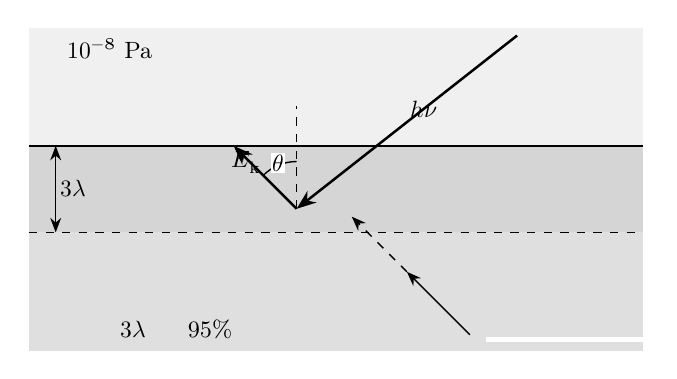
\begin{tikzpicture}[x=1mm,y=1mm,>=Stealth]
% 气相
\fill[gray!12] (0,0) rectangle (78,15);
% 固体
\fill[gray!25] (0,-26) rectangle (78,0);
% 采样深度带
\fill[gray!45,opacity=0.40] (0,-11) rectangle (78,0);
\draw[mainline] (0,0) -- (78,0);
\draw[dashed,thinline] (0,-11) -- (78,-11);
\draw[<->,thinline] (3.4,0) -- (3.4,-11)
  node[midway,right,inner sep=1.5pt] {$3\lambda$};
% 气相说明
\node[anchor=north west,text width=40mm,align=left,inner sep=1pt] at (2,14)
  {气相（$10^{-8}$ Pa 量级）：出射电子不与气体分子碰撞};
% 入射 X 射线
\draw[->,mainline] (62,14) -- (34,-8) node[midway,above right,inner sep=1pt] {$h\nu$};
% 法线与出射电子
\draw[dashed,thinline] (34,-8) -- (34,5);
\draw[->,mainline] (34,-8) -- (26,0)
  node[midway,above left,inner sep=1pt] {$E_{\mathrm{k}}$};
\draw[thinline] (34,-2) arc[start angle=90,end angle=135,radius=6];
\node[fill=white,inner sep=0.5pt] at (31.6,-2.2) {$\theta$};
% 深部电子：非弹性散射后无法逃出
\draw[->,thinline] (56,-24) -- (48,-16);
\draw[->,thinline,dashed] (48,-16) -- (41,-9);
\node[anchor=south west,text width=20mm,align=left,inner sep=1pt,fill=white]
  at (58,-25) {深部电子：非弹性散射失去能量，成为连续本底};
% 采样深度带说明
\node[anchor=south west,text width=34mm,align=left,inner sep=1pt] at (1,-25)
  {采样深度带：法向出射时 $3\lambda$ 内贡献约 95\% 信号};
\node[anchor=east,inner sep=1pt] at (76.5,-2.6) {固体};
\end{tikzpicture}
\caption{表面分析信号来源与逃逸深度示意。读者应看三处：① 入射 X 射线穿透约 1000 nm，远大于
电子的逃逸深度，信息深度由\textbf{电子}而非光子决定；② 只有采样深度带内产生、且沿出射方向未
发生非弹性散射的电子才形成弹性峰，其信息深度为 $d=3\lambda\cos\theta$；③ 更深处产生的电子经
非弹性散射后成为连续本底，本底随结合能升高而抬高。图中厚度与角度按可读性缩放，$\lambda$ 取
$3\lambda$ 带的 $1/3$。\schemamark\figsrc{据 S2 图 9-16，书内 p.582 / PDF p.73 改绘。}}
\label{fig:escape}
\end{figure}

$\lambda$ 与电子动能的关系不是单调的：约 50—100 eV 处取最小值（约 0.5 nm），向低能端与高能端
都上升。这带来一个实用推论：芯能级光电子的动能高（如 Al K$\alpha$ 激发的 C 1s 光电子约
1198 eV，$\lambda\approx1.1$ nm），采样深度较大；而俄歇电子的动能只有几百 eV，$\lambda$ 更小
（C KVV 约 270 eV 时 $\lambda\approx0.6$ nm），所以\textbf{俄歇峰的信息深度通常比同一元素的
芯能级光电子峰更浅}。

各种材料的采样深度粗略估计为：金属 $0.5$—$2$ nm，无机化合物 $1$—$3$ nm，有机物 $3$—$10$ nm。
还需记住：同一元素的不同能级、以及换用不同激发源，都会改变出射电子的动能，从而改变 $\lambda$
与采样深度——同一张谱上不同峰的表面灵敏度并不相同。
\src{S2 §9.2.2，书内 p.583 / PDF p.74，图 9-17}

\subsubsection{由信息深度决定的方法分工}

常见表面分析技术的原理与所获信息不同：\term{XPS}{X-ray photoelectron spectroscopy}{X 射线
光电子能谱}用 X 射线光子激发芯能级电子、测其动能以确定结合能，给出元素组成与化学态；
\term{AES}{Auger electron spectroscopy}{俄歇电子能谱}改用千电子伏电子束轰击，主要给元素组成
而束斑可以很小；\term{UPS}{ultra-violet photoelectron spectroscopy}{紫外光电子能谱}以紫外
光子激发价电子，给价带谱、功函数与费米能级信息；%
\term{SIMS}{secondary ion mass spectroscopy}{二次离子质谱}以高能离子束溅射、用质谱分析二次
离子，灵敏度极高且可测氢。XPS、UPS、AES 与 ISS 可在同一台谱仪中实现，共用一个分析器。
信息深度上 XPS、UPS、AES 为 $0.5$—$10$ nm，ISS 只有单层，SIMS 覆盖 $0.5$—$300$ nm，
AFM/STM 只给最上层原子的形貌、不给化学态；元素范围也不同（XPS/AES/UPS 为 Li—U，SIMS 为 H—U）。
应用时应记住两条原则：先弄清材料特性、所需信息与手段的能力和局限；不要奢望仅用一种技术满足
全部需求。\src{S2 §9.1，书内 p.569、p.571—573 / PDF p.60、p.62—64，表 9-4、图 9-1}

\begin{crosscheck}
表面敏感技术回答「最外层有什么、以什么价态存在」，不回答「体相是什么晶相、内部长什么样」：
后者要靠 \chapref{ch:04} 的 XRD 补体相晶相、靠 \chapref{ch:02} 的 TEM/EDS 补形貌与体相微区
成分、靠 \chapref{ch:05} 的化学吸附与程序升温方法补活性位与氧化还原行为。同为表面敏感的方法
之间也要互相回查：AES 束斑小、可扫描成像，但电子束损伤远大于 X 射线；UPS 给价带与功函数，
不给芯能级化学态；SIMS 灵敏度极高且可测氢，但定量困难、同样有溅射损伤；ISS 只给最外层原子。
定量结果还应用独立方法（XRF、ICP、EDS）的体相组成核对——两者的差异本身往往是信息（表面富集
或偏析），而不是哪一方「测错了」。
\end{crosscheck}

\subsection{X 射线光电子能谱（XPS）}

XPS 全称为 X-ray photoelectron spectroscopy，早期也称 ESCA（electron spectroscopy for
chemical analysis，化学分析用电子能谱），是用电子能谱仪测量 X 射线光子辐照样品表面所产生的
光电子与俄歇电子能量分布的方法。\src{S2 §9.2，书内 p.573 / PDF p.64}

\subsubsection{历史进程（导航保留）}

从 Hertz、Hallwachs 的观察（19 世纪 80 年代至 1888 年）到 Einstein 1905 年用能量量子化解释
光电效应，物理图像在 20 世纪初已经确立；1954 年 K. M. Siegbahn 制成世界上第一台光电子能谱
设备（Cu K$\alpha_{1}$ 源，$\lambda=0.15418$ nm，$h\nu\approx8042.6$ eV），精确测定了元素
周期表中各种原子的内层电子结合能。真正让它进入表面科学的是 20 世纪 60 年代的发现：硫代硫酸钠
中 \ce{S^{6+}} 与 \ce{S^{2-}} 的 S 2p 结合能相差约 6 eV，即\textbf{原子内层电子结合能的变化
可以提供分子结构与化学态的信息}——这是 XPS 的立命之本，K. M. Siegbahn 因此获 1981 年诺贝尔
物理学奖。仪器型号与人物沿革不再展开，需要时可回查原书图 9-2—图 9-8。
\src{S2 §9.2.1，书内 p.573—577 / PDF p.64—68}

\subsubsection{基本原理}

\paragraph{光电效应与基本方程}

\begin{principle}
XPS 的基本原理就是光电效应（光致发射、光电离）：样品被特征能量的光子辐照，测量出射光电子的
动能，从中获得所需信息。原子中不同能级上的电子具有不同的结合能；当一束能量为 $h\nu$ 的入射
光子与样品中的原子相互作用时，单个光子把全部能量交给原子中某壳层（能级）上一个受束缚的
电子。如果光子能量大于该电子的结合能，电子就脱离原来受束缚的能级，剩余能量转化为动能并以
一定动能从原子中发射出去成为自由电子，原子本身则成为激发态的离子。从激发到发射的过程极快
（约 $10^{-16}$ s），其能量守恒关系即爱因斯坦方程 \equref{eq:xps}。
\end{principle}

\begin{equation}\label{eq:xps}
E_{\mathrm{k}}=h\nu-E_{\mathrm{B}}-\phi_{\mathrm{sp}}
\end{equation}

式中 $E_{\mathrm{k}}$ 为出射光电子的动能，eV；$h\nu$ 为 X 射线源光子的能量，eV；
$E_{\mathrm{B}}$ 为特定原子轨道上的结合能，eV；$\phi_{\mathrm{sp}}$ 为谱仪的功函数，eV，主要由
谱仪材料与状态决定，对同一台谱仪基本是一个常数、与样品无关，平均值 $3$—$5$ eV。移项即得
$E_{\mathrm{B}}=h\nu-E_{\mathrm{k}}-\phi_{\mathrm{sp}}$：实测的是动能，报告的是结合能，中间的
$\phi_{\mathrm{sp}}$ 只能靠标定消去。\src{S2 §9.2.2，书内 p.579 / PDF p.70，式(9-1)}

\begin{keycond}
\equref{eq:xps} 的成立条件：① 样品与谱仪有良好电接触并共同接地，使二者费米能级处于同一能级
（导电样品，原书图 9-11）；绝缘样品做不到这一点，谱线会整体漂移（原书图 9-12）；② $h\nu$ 为
单一能量；③ $\phi_{\mathrm{sp}}$ 在同一台谱仪、同一工作状态下视为常数；④ 该式只描述单电子
电离的能量守恒，不含终态弛豫对峰位与峰形的修正。量纲检查：$h\nu$、$E_{\mathrm{B}}$、
$E_{\mathrm{k}}$、$\phi_{\mathrm{sp}}$ 全部是能量，取同一单位（eV）即可，式中没有需要标定的
系数；若改用 J 只需统一换算（$1$ eV $=1.602\times10^{-19}$ J）。极限情况：当
$h\nu<E_{\mathrm{B}}+\phi_{\mathrm{sp}}$ 时无光电子出射——这给出 XPS 可测能级的硬边界。
\end{keycond}

\paragraph{两条标定路线}由 \equref{eq:xps} 可见，$\phi_{\mathrm{sp}}$ 与样品荷电都会让整条谱线
一起平移，因此实测谱必须先标定，而且要把两件事分开。\textbf{谱仪能量标尺标定（仪器问题）}：
用 Au 4f$_{7/2}$、Cu 2p$_{3/2}$、Ag 3d$_{5/2}$ 等金属标样在同一台谱仪上测量，把已知结合能对准，
以消去 $\phi_{\mathrm{sp}}$ 与标尺的非线性。\textbf{样品荷电标定（样品问题）}：绝缘样品的荷电
使全部峰一起平移，必须用中和枪并把一个已知位置的峰调到指定值；最常用的是污染碳 C 1s 取
$284.8$ eV——它几乎无处不在、与样品处于同一荷电状态、一次录谱就能得到，代价是污染碳自身的
结合能随真空、样品与荷电状态在约 $284.5$—$285.0$ eV 之间漂移，用它定标等于把这个不确定度
转移给全部峰。两者不能互相替代：蒸镀 Au 做内标可辅助判断荷电，但只有 Au 与样品处于同一电位时
才成立。\tocheck{未对照原页面图像：Au 4f$_{7/2}$ 约 $84.0$ eV 与污染碳 C 1s $284.8$ eV 均为
通用标定值，分片 a 的源文本未给出这些数值，需与后续分片或原书核对后再作为书上给出的值引用。}

可被激发的能级还受 $h\nu$ 限制：常用 Mg K$\alpha$（$1253.6$ eV）与 Al K$\alpha$
（$1486.6$ eV）只能激发出结合能小于 $h\nu-\phi_{\mathrm{sp}}$ 的壳层。以金为例，Al K$\alpha$
下最深的可测能级是 4s，更内层的能级无法激发；H 与 He 没有内层电子，XPS 无法测量，所以 XPS 的
元素范围下限是 Li。

\paragraph{弛豫：X 射线荧光与俄歇电子}电离产生的终态离子不稳定、处于高激发态，会自发弛豫
（退激发）而变为稳态，弛豫分辐射弛豫与非辐射弛豫两种：前者发射 X 射线荧光，后者发射俄歇电子。
以 X 射线光子把能量转移给芯能级电子为例（原书图 9-15）：（a）从 $n$ 电子初态发生光电发射，
即光电子出射；（b）处于 $(n-1)$ 电子状态的原子通过把更高能级的电子退到空穴而重排；（c）重排
释放的能量可以交给另一个电子使其发射，这个电子就是俄歇电子，也可以以 X 射线光子的形式释放。
由此得到一条极有用的判别依据：\textbf{光电子峰的表观位置随 $h\nu$ 移动，而俄歇峰的动能由原子
自身能级决定、与 $h\nu$ 无关}。换靶复测（例如 Mg K$\alpha$ 换 Al K$\alpha$）时，位置不动的是
光电子峰，位置移动的是俄歇峰——这既是识别未知峰的判据，也是排除 X 射线卫星线的判据
（图~\ref{fig:xpsspec}）。\src{S2 §9.2.2，书内 p.581—582 / PDF p.72—73，图 9-15}

\begin{figure}[tbp]
\centering
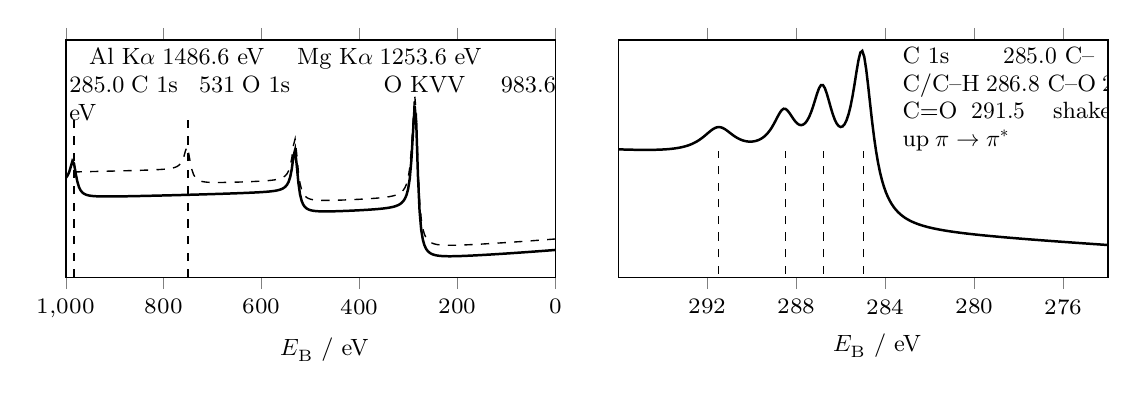
\begin{tikzpicture}
\begin{groupplot}[
  group style={group size=2 by 1, horizontal sep=8mm},
  width=78mm, height=46mm,
  x dir=reverse, ymin=0, ytick=\empty, scaled ticks=false,
]
\nextgroupplot[xmin=0, xmax=1000, ymax=2.6, xtick={0,200,400,600,800,1000},
  xlabel={结合能 $E_{\mathrm{B}}$ / eV}, ylabel={强度（任意单位）}]
\addplot[domain=0:1000,samples=300,mainline,black]{0.30*exp(-x/700)
+1.00/(1+((x-285)/6)^2)+0.35/(1+((x-287.5)/6)^2)+0.12/(1+((x-291.5)/6)^2)
+0.55/(1+((x-531)/7)^2)+0.30/(1+((x-983.6)/8)^2)
+0.21*(1+(x-285)/sqrt((x-285)^2+9))+0.05*(1+(x-287.5)/sqrt((x-287.5)^2+9))
+0.02*(1+(x-291.5)/sqrt((x-291.5)^2+9))+0.12*(1+(x-531)/sqrt((x-531)^2+9))
+0.08*(1+(x-983.6)/sqrt((x-983.6)^2+9))};
\addplot[domain=0:1000,samples=300,thinline,black,dashed]{0.12+0.30*exp(-x/700)
+1.00/(1+((x-285)/6)^2)+0.35/(1+((x-287.5)/6)^2)+0.12/(1+((x-291.5)/6)^2)
+0.55/(1+((x-531)/7)^2)+0.30/(1+((x-750.6)/8)^2)
+0.21*(1+(x-285)/sqrt((x-285)^2+9))+0.05*(1+(x-287.5)/sqrt((x-287.5)^2+9))
+0.02*(1+(x-291.5)/sqrt((x-291.5)^2+9))+0.12*(1+(x-531)/sqrt((x-531)^2+9))
+0.08*(1+(x-750.6)/sqrt((x-750.6)^2+9))};
\draw[dashed,thinline] (axis cs:983.6,0) -- (axis cs:983.6,1.80);
\draw[dashed,thinline] (axis cs:750.6,0) -- (axis cs:750.6,1.80);
\node[anchor=north west,text width=74mm,align=left,inner sep=1pt] at (axis cs:1000,2.55)
  {实线：Al K$\alpha$（1486.6 eV）；虚线：Mg K$\alpha$（1253.6 eV，为便于分辨整体上移 0.12）。
  换靶后 285.0（C 1s）与 531（O 1s）两个弹性峰位置不动，俄歇 O KVV 峰则由 983.6 移到
  750.6 eV。};
\nextgroupplot[xmin=274, xmax=296, ymax=1.35, xtick={276,280,284,288,292},
  xlabel={结合能 $E_{\mathrm{B}}$ / eV}]
\addplot[domain=274:296,samples=250,mainline,black]{0.18+0.008*(x-274)
+0.85/(1+((x-285)/0.55)^2)+0.45/(1+((x-286.8)/0.6)^2)+0.25/(1+((x-288.5)/0.65)^2)
+0.15/(1+((x-291.5)/0.9)^2)
+0.10*(1+(x-285)/sqrt((x-285)^2+0.09))+0.05*(1+(x-286.8)/sqrt((x-286.8)^2+0.09))
+0.03*(1+(x-288.5)/sqrt((x-288.5)^2+0.09))};
\draw[dashed,thinline] (axis cs:285,0.02) -- (axis cs:285,0.72);
\draw[dashed,thinline] (axis cs:286.8,0.02) -- (axis cs:286.8,0.72);
\draw[dashed,thinline] (axis cs:288.5,0.02) -- (axis cs:288.5,0.72);
\draw[dashed,thinline] (axis cs:291.5,0.02) -- (axis cs:291.5,0.72);
\node[anchor=north west,text width=33mm,align=left,inner sep=1pt] at (axis cs:283.4,1.33)
  {C 1s 分峰（示意）：$285.0$ C--C/C--H；$286.8$ C--O；$288.5$ C=O；
  $291.5$ 伴峰（shake-up，$\pi\rightarrow\pi^{*}$）};
\end{groupplot}
\end{tikzpicture}
\caption{模型计算的 XPS 谱示意。(a) 全谱：同一含碳含氧样品在 Al K$\alpha$（实线）与
Mg K$\alpha$（虚线，为便于分辨整体上移 0.12）激发下的谱形，读者应看三处：① 连续本底随结合能
升高而抬高，来自非弹性散射电子（成因见图~\ref{fig:escape}）；② 弹性峰（C 1s 285.0 eV、
O 1s 531 eV）在换靶后峰位不动；③ 俄歇 O KVV 峰的表观结合能由 983.6 eV 变为 750.6 eV，
即随激发光子能量移动。(b) C 1s 窄区放大：主峰 285.0 eV，化学位移峰 286.8 与 288.5 eV，
高结合能侧 291.5 eV 的 $\pi\rightarrow\pi^{*}$ 伴峰（shake-up）。(a) 的横轴按 XPS 惯例由右向左
增大。峰形取洛伦兹型 $A/[1+((E_{\mathrm{B}}-p)/w)^2]$（$w=6$—8 eV，为可读性放大），本底为
指数衰减项 $B_{0}e^{-E_{\mathrm{B}}/700}$ 加各峰下的阶跃项；峰位、峰宽与强度均为示意设定，
不代表任何实测样品。\modelmark}
\label{fig:xpsspec}
\end{figure}

\paragraph{能级标记与自旋轨道分裂}原子中单个电子的运动状态用量子数 $n,l,m_{l},m_{s}$ 描述：
$n$ 为主量子数，能量主要取决于它，$n=1,2,3,4,\dots$ 对应 K、L、M、N 壳层；$l$ 为角量子数，
$l=0,1,2,3,\dots$ 对应 s、p、d、f 能级；$m_{l}$ 决定电子云取向；$m_{s}$ 为自旋量子数，取
$\pm1/2$。轨道运动与自旋运动之间的耦合使能级分裂，当 $l>0$ 时用内量子数 $j$ 表示：

\begin{equation}\label{eq:jsplit}
j=|l\pm1/2|
\end{equation}

所以 $l=0$ 时 $j=1/2$（s 能级不分裂），$l>0$ 时 $j=l+1/2$ 或 $l-1/2$，在谱图上表现为双峰，
如 Ag 3d$_{5/2}$ 与 3d$_{3/2}$；s 能级的内量子数 $1/2$ 通常省略，如 C 1s 只有一个峰。XPS 一般
采集芯（内）能级谱（C 1s、Al 2p、Ag 3d、Au 4f 等），因为这些谱线强度强、分辨好。双峰的面积比
由简并度 $2j+1$ 决定，即 $p$ 为 $2\!:\!1$、$d$ 为 $3\!:\!2$、$f$ 为 $4\!:\!3$——这是判断
双峰是否成对、以及是否有物种被漏掉的独立约束。
\src{S2 §9.2.2，书内 p.584—585 / PDF p.75—76，表 9-5、图 9-18}

\paragraph{光致电离截面与灵敏度因子}光电效应的概率用光致电离截面 $\sigma$ 表示，定义为某能级
的电子对入射光子的有效能量转移面积，或一定能量的光子从某个能级激发出一个光电子的概率。入射
光子能量一定时有如下规律：① 同一原子中半径越小的壳层 $\sigma$ 越大；② 电子结合能与入射光子
能量越接近 $\sigma$ 越大；③ 不同原子中同一壳层，原子序数越大 $\sigma$ 越大。$\sigma$ 越大，
该能级的光电子峰强度就越大。常用的数据库有两个：Scofield 理论光致电离截面（基于 C 1s $=1$）
与 Wagner 实验灵敏度因子（基于 F 1s $=1$），各谱仪厂商的因子库都源自这两个数据源。这决定了
一条纪律：\textbf{定量时必须声明用了哪一套因子、基准是什么}，两套混用会带来系统性偏差。
XPS 的表面检测灵敏度可达 $10^{-3}$ 原子单层，但对体相检测的灵敏度只有 0.1\% 左右。
\src{S2 §9.2.2，书内 p.585—586 / PDF p.76—77，表 9-6、图 9-19}
\tocheck{未对照原页面图像：原 OCR 作「可以达到 103 原子单层」，上标负号丢失；按通行表述重建为
$10^{-3}$ 原子单层，需与书内 p.586 原页核对。}

\paragraph{从谱图到结论}

\begin{dataflow}
一条完整的判读链是：录谱（全谱定元素，目标元素窄谱定化学态）$\rightarrow$ 校准（谱仪标尺用
Au 4f$_{7/2}$ 等标样，样品荷电用内标或中和枪）$\rightarrow$ 扣背景（Shirley 或线性，扣法直接
改变峰面积）$\rightarrow$ 分峰拟合（约束峰形、半高宽上限、双峰间距与面积比）$\rightarrow$ 用
相对灵敏度因子把峰面积换算为原子百分比 $\rightarrow$ 与参考态（同批标准样品或数据库）比对给出
化学态。每一步都留下假设：标定物必须与样品处于同一荷电状态；背景扣法影响面积从而影响定量；
拟合约束必须写明，否则分出的物种不可复核；定量只给相对含量，且以采样深度内组成均匀为前提。
\end{dataflow}

\begin{obs}
\pedset{教学设定数值}某 Ni 基样品的 Ni 2p$_{3/2}$ 主峰实测结合能为 $855.4$ eV，在高结合能侧
约 $+6$ eV 处有一个宽的卫星峰；同一谱中污染碳 C 1s 位于 $284.8$ eV。样品在空气中放置一周后
重复测量，主峰移到 $856.2$ eV，而卫星峰与主峰的间距不变、峰形也无明显变化。
\end{obs}

\begin{infer}
峰位移动而双峰间距、卫星峰结构与峰形不变，说明这次移动来自荷电或标定条件的整体变化，而不是
Ni 的价态改变。若要把 $855.4$ eV 归属为某一价态，前提是：① 谱仪标尺已用金属标样校准；
② 荷电校准所用内标与样品同电位；③ 与同批参考态（金属 Ni、NiO 等）在同一条件下测得并对比。
三条缺一，峰位就只能写成「与某参考态接近」，不能作为价态的唯一证明。
\end{infer}

\subsubsection{仪器与主要组成部件}

XPS 仪器由配套的高、超高真空系统，电子能量分析器与探测器，激发源（XPS 用 Mg/Al 双阳极或
单色化 Al K$\alpha$ 源，AES 用电子枪，UPS 用紫外光源，ISS 用离子源），低能离子源，电子中和枪，
多自由度样品架，以及仪器控制与数据采集处理系统等组成。这些部件不是可选项的堆叠，而是围绕
「让少量低能电子在无场、无碰撞、无荷电干扰的条件下被计数」这一目标互相约束的整体
（表~\ref{tab:xpsparts}）。\src{S2 §9.2.3，书内 p.586—605 / PDF p.77—96，图 9-20、图 9-21}

\begin{table}[tbp]
\centering
\caption{XPS 谱仪的主要组成部件、常见形式与使用要点}
\label{tab:xpsparts}
{\srcsize
\begin{tabularx}{\twocolwidth}{@{}l p{56mm} X@{}}
\toprule
部件 & 常见形式与典型取值 & 使用要点 \\
\midrule
真空系统 & 快速进样室（$10^{-3}$ Pa 量级）、样品制备室、分析室（$10^{-8}$ Pa 量级）；旋片式
机械泵、涡轮分子泵组、溅射离子泵、钛升华泵 & 三室之间用大口径隔离阀与传输机构；分析室腔体用
$\mu$ 合金（Fe18/Ni75/Cr2/Cu5）屏蔽外磁场；压强低于设定值才允许开启各激发源 \\
X 射线源 & Mg/Al 双阳极：Mg K$\alpha$ $1253.6$ eV、线宽 $0.7$ eV，Al K$\alpha$
$1486.6$ eV、线宽 $0.85$ eV；单色化 Al K$\alpha$ 源（$\alpha$-石英 $10\bar{1}0$ 面，罗兰圆
半径常取 $250$ mm） & 非单色源带 K$\alpha_{3}$、K$\alpha_{4}$、K$\beta$ 卫星线与强的韧致辐射
本底，常用约 $2$ $\mu$m 的 Al 箔滤去大于 $1.5$ keV 的连续背景；单色化后线宽可降至约
$0.25$ eV，并可得小束斑，便于小面积、线扫描与成像 \\
电子能量分析器 & 静电场型半球 $180^{\circ}$ 分析器（SCA），常见直径 $220$—$450$ mm；外壳
双层 $\mu$ 合金 & 同心半球加 $\Delta V$（外半球为负），只有一定能量范围的电子能到达出口；
XPS 用 FAT/CAE 模式（绝对分辨率恒定、检测效率一致，适合面积法定量），AES 与 UPS 可用
FRR/CRR 模式 \\
透镜与传输 & 收集（预减速）透镜、多级静电透镜，可切换减速比 & 分辨能力与传输特性互相矛盾。
预减速后动能由 $E_{0}$ 降到 $E_{0}'$，分析器只需满足 $R_{b}'=(E_{0}/E_{0}')R_{b}$，系统
分辨率不变而分析器尺寸不必加大；同时拉开样品与分析器距离，减少次级电子本底 \\
探测器 & 单通道电子倍增器（增益 $10^{6}$—$10^{9}$）、$3/6/7/9$ 管阵列、微通道板（MCP），
多至 256 通道 & 待测电子流只有 $10^{-11}$—$10^{-8}$ A；阵列沿能量色散方向排列，输出按能量
移位后相加可提高灵敏度；MCP 单通道增益远低于单通道倍增器，不能只按通道数比较灵敏度 \\
荷电中和 & 早期为单束低能电子枪，现在多用低能 \ce{Ar+} 与低能电子束的双束中和 & 作用是减小
绝缘样品表面荷电，使作为内标的峰回到指定位置；还须消除荷电不均匀，否则会出现多重裂分谱峰，
被误读成「多种化学态」 \\
离子枪与样品架 & 差分抽气细聚焦扫描型（置于分析室）、大束斑高速型（置于制备室）；\ce{Ar}
团簇离子枪（团簇含 $2000$—$3600$ 个 \ce{Ar} 原子）；多自由度样品架 & 单 \ce{Ar+} 束轰击会
破坏表面状态，对有机物与聚合物尤甚；团簇源把初始动能分摊到上千个原子上，冲击能量低、损伤小。
变角分析要求样品面与样品架 $x$ 轴轴心共面 \\
\bottomrule
\end{tabularx}}
\figsrc{据 S2 §9.2.3，书内 p.586—605 / PDF p.77—96，图 9-20—图 9-42 整理。}
\end{table}

\paragraph{四点必要说明}① \textbf{真空}：三室分别负责快速进样、样品预处理与主分析，把热处理、
蒸镀、刻蚀等「脏活」放在制备室是为了保住分析室的 $10^{-8}$ Pa；泵有层级（旋片泵作前级，
涡轮分子泵或溅射离子泵作主泵，钛升华泵辅助），且只有压强低于设定值时联锁才允许开启激发源，
以保护灯丝、阳极靶与样品。② \textbf{分析器模式}：FAT/CAE 把进入分析器的电子减速到固定通能，
因 $\Delta E/E$ 中的 $E$ 固定而整条标尺上绝对分辨率不变，通能越低分辨越好但信号越弱（窄谱
$5$—$25$ eV、全谱 $100$—$200$ eV）；FRR/CRR 的 $\Delta E/E$ 恒定，但通能随能量变化、检测
效率不同，不利于定量，故 XPS 不用，而适合 AES 的峰对峰高度法与 UPS。③ \textbf{X 射线源}：
高能电子束撞击阳极产生内空穴并发射荧光 X 射线与韧致辐射，特征线能量固定；双阳极源通量高，
但带卫星线、次级电子本底、样品降解与灯丝沾污，故常用 Al 箔滤去大于 $1.5$ keV 的连续背景；
更好的办法是单色化——$\alpha$-石英 $10\bar{1}0$ 面间距 $0.425$ nm，对波长 $0.834$ nm 的
Al K$\alpha$ 线在 $78.5^{\circ}$ 处满足布拉格方程

\begin{equation}\label{eq:bragg-ch09}
n\lambda=2d\sin\theta
\end{equation}

数值核对：$2\times0.425\times\sin78.5^{\circ}=0.833$ nm，与 $0.834$ nm 相差约 0.1\%，自洽。
单色化可把 Al K$\alpha$ 线宽从 $0.85$ eV 降至约 $0.25$ eV，消除 K$\alpha_{3}$、K$\alpha_{4}$
伴峰与韧致辐射本底，并取得小束斑。④ \textbf{探测与中和}：待测电子流只有 $10^{-11}$—$10^{-8}$ A，
靠电子倍增器计数；中和枪减小绝缘样品荷电、使内标峰回到指定位置，并消除荷电不均匀（否则多重
裂分谱峰会被误读为多种化学态）。
\src{S2 §9.2.3，书内 p.588—604 / PDF p.79—95，图 9-21—图 9-42}
\tocheck{未对照原页面图像：原书（书内 p.604）称绝缘样品表面「负电荷富集」，而按光电发射过程，
绝缘样品通常因电子出射而带正电，这也是中和枪要提供低能电子的原因；两种说法方向相反。分片 a
只保留「中和不足或过度都会留下荷电」这一结论，不判断原书是否有误，请以原页面图像复核。}

\subsubsection{XPS 实验方式}

传统 XPS 给出固体表面某一小区域的元素组成、化学态与元素相对含量；现代 XPS 还能提供元素及其
化学态的横向与纵向（深度）分布，即线扫描、深度剖析与成像。常规点分析可使用 Mg-Al 双阳极或
单色化 X 射线源；用单色化源再配合分析器透镜部分的光阑，可实现小面积分析，目前最小采样面积
直径可小至 $9$ $\mu$m。

\paragraph{深度剖面：破坏性与非破坏性两条路线}破坏性方法用于获取深于 10 nm 的组分变化信息，
非破坏性方法只能给出表面 $1$—$10$ nm 内的组成变化。

\emph{离子刻蚀（破坏性）}先用常规方法分析原始表面，再以几百 eV 至几千 eV 的离子束刻蚀一定
时间、停止刻蚀并测谱，如此循环至所需深度。聚焦离子束斜向作用于表面，刻蚀坑不可能均匀，
特别是坑的边缘会使深度数据产生偏差，故要求刻蚀区域大于 XPS 采集出射光电子的范围并使用可旋转
样品托；最理想的刻蚀面积是测试面积的 100 倍，以确保测试区处于坑中心的平坦位置。刻蚀后的新鲜
表面极其敏感，须用高纯或超纯 \ce{Ar} 并注意系统残余气氛，否则新鲜表面的化学组成会被改变。
刻蚀深度用已知准确厚度的薄膜标样标定：常用的 \ce{Ta2O5}/Ta 标样由阳极化工艺制得、层厚控制
精确，例如 $30$ nm 标样的氧化层厚度就是 O 1s 与 Ta 4f$_{7/2}$ 强度-溅射时间曲线中Ⅰ段、Ⅱ段
与Ⅲ段 50\% 之和在横坐标上的投影段。副效应必须逐条记住：\textbf{择优溅射}（各元素溅射系数
不同，合金的新表面组成偏离原始组成）、热效应、离子注入、\textbf{表面局部被还原}（硝酸盐、
磷酸盐、碳酸盐在 $1$—$3$ keV \ce{Ar+} 轰击下可转化为氧化物，高价态氧化物最易被还原）、粗糙度
增加、表层重构（聚合物尤明显）与污染分析室。因此刻蚀应选低能离子束，大面积、长时间的清洁尽量
在制备室进行；对有机物与聚合物宜改用 \ce{Ar} 团簇离子源（团簇含 $2000$—$3600$ 个 \ce{Ar}
原子），初始动能分摊到上千个离子上，冲击能量低、化学破坏小。

\emph{变角 XPS（非破坏性）}XPS 测得的表面信息其实是表面与近表面多层信息的叠加，来自各层的
信息不同，这正是变角深度分析的基本概念：改变样品面的倾斜角度即精确改变出射角，利用采样深度与
出射角的关系得到元素浓度与深度的关系，

\begin{equation}\label{eq:arxps}
d^{*}=d\cos\theta=3\lambda\cos\theta
\end{equation}

式中 $\theta$ 为出射角（进入分析器方向的出射电子与样品法线的夹角），$\lambda$ 为非弹性散射
平均自由程；\equref{eq:arxps} 与 \equref{eq:sampling-depth} 是同一关系，只是写成随角度变化的
采样深度 $d^{*}$。$\theta=0^{\circ}$ 时采样最深，增大 $\theta$ 可获得更多表面层信息，
$\theta=85^{\circ}$ 时表面灵敏度提高约 10 倍（$\cos85^{\circ}\approx0.087$）。变角 XPS
（\term{ARXPS}{angle-resolved XPS}{变角 XPS}）只适用于表面层很薄（$1$—$10$ nm）的体系，
使用时还须注意：单晶表面的点阵衍射效应、表面粗糙度、样品面与样品架 $x$ 轴轴心共面、绝缘样品
荷电补偿随角度的变化（同样适用于 \ce{Ar+} 刻蚀剖面）、以及录谱范围要能容纳化学位移幅度。
与此相关的一种新方法是平行探测（结合位敏探测器）：由传输透镜、半球分析器与二维探测器
（微通道板）结合，在一个平面上收集能量色散信息、在另一平面收集角分布信息，不转动样品即可获得
大于 $60^{\circ}$ 范围的角度分布数据，得到无损的浅层化学态深度分布，且分析面积与荷电补偿不变。

\paragraph{线扫描与成像}用小束斑单色化 X 射线源，让细聚焦 X 射线束在样品表面线性移动（或束
固定、样品移动），可测得元素及其化学态的线强度分布；让束作 X-Y 扫描即得分布图。成像方式主要有
四种：扫描阳极使细 X 光束在样品上扫描、计算机控制样品台作 X-Y 扫描、在分析器透镜中间加静电
偏转板作光电子束扫描，以及平行（照相式）成像——后者每个像素都含一个完整谱，峰拟合后可再现
化学态的空间分布。
\src{S2 §9.2.4，书内 p.605—614 / PDF p.96—105，图 9-43—图 9-56}

\begin{measure}
录谱与校准的可操作条件：① \textbf{通能}：高分辨窄谱 $5$—$25$ eV，全谱 $100$—$200$ eV；
模式选 FAT/CAE，因为它的绝对分辨率在整条标尺上恒定、检测效率一致，可作面积法定量。
② \textbf{校准分两步}：先用 Au 4f$_{7/2}$、Cu 2p$_{3/2}$、Ag 3d$_{5/2}$ 等金属标样校准谱仪
能量标尺，再处理样品荷电——绝缘样品用中和枪并把内标（污染碳 C 1s 取 $284.8$ eV）调到指定
位置，且标定物与样品必须处于同一荷电状态。③ \textbf{深度剖析}：离子能量尽量低；刻蚀面积
不小于测试面积的 100 倍并用可旋转样品托；用高纯 \ce{Ar}；刻蚀速率用 \ce{Ta2O5}/Ta 标准样
标定；有机物与聚合物改用团簇离子源。④ \textbf{变角分析}：表面层厚度小于 10 nm；样品面与
样品架 $x$ 轴轴心共面；绝缘样品要检查荷电补偿随角度的变化。⑤ \textbf{定量}：同一批数据只用
一套相对灵敏度因子（Scofield 基准 C 1s $=1$，或 Wagner 基准 F 1s $=1$）并写明基准。
\end{measure}

\begin{pitfall}
\textbf{① 荷电效应冒充化学位移。}绝缘样品上，X 射线激发的电子发射与中和枪注入的电子并不总能
平衡，表面会留下净电荷。由 \equref{eq:xps} 可直接看出：表面带正电时出射电子被减速、实测动能
偏低，表观结合能偏高；中和过度则表观结合能偏低。判别办法不是看单个峰而是看整体：荷电使
\textbf{全部元素的峰一起平移}，且平移量随 X 射线通量、采集时间或中和条件改变；真实的化学位移
只影响价态发生变化的那些元素，且自旋轨道分裂间距、卫星峰结构与峰形会随峰位一起变化，并在
改变通量或中和条件后可以重现。荷电不均匀还会造成峰形展宽甚至多重裂分，把「一种化学态」读成
「多种化学态」——这时应先怀疑中和，而不是先加分峰。

\textbf{② X 射线还原样品。}非单色源的高能韧致辐射、次级电子与热量都可能使样品降解：高价态
氧化物、硝酸盐、磷酸盐、碳酸盐最易被还原（\ce{Ar+} 刻蚀有同样的还原作用）。判据是\textbf{时间
序列}：若连续录谱中高价态峰单调减弱、低价态峰单调增强，首先应怀疑辐照损伤，而不是「发现了新
物种」；降低通量、缩短单次采集、改用单色化源后变化减小，即可确认。

\textbf{③ 污染碳干扰。}真空残余的碳氢化合物在 X 射线或电子束下裂解沉积到表面，表现为 C 1s
随时间增长（常伴 O 1s）。危害有两层：若样品本身含碳，污染碳会掩盖真实碳物种；若用污染碳作
内标，则把它自身约 $284.5$—$285.0$ eV 的不确定度转移给全部峰。判别办法是比较新解理或刚刻蚀
完的表面与放置一段时间后的 C 1s 强度。

\textbf{④ 深度不均匀导致定量偏差。}相对灵敏度因子定量以「采样深度内组成均匀」为前提。核壳
结构、表面富集或偏析、刻蚀坑边缘的信号混合都会破坏这个前提：前者使表面组成不能代表整体，
后者把界面「展宽」成渐变层。自检办法有两个：做变角测量，峰强度比随出射角变化即说明深度不均
匀；或用同一元素动能差别较大的两个峰分别定量，结果不一致同样说明不均匀。此时定量只能表述为
「在 $3\lambda$ 深度内的相对含量」。
\end{pitfall}
}{}
\IfFileExists{chapters/parts/ch09-b.tex}{% ================================================================
%  chapters/parts/ch09-b.tex
%  第 9 章 表面分析技术基础（分片 b）
%  源：S2（下册）§9.2.5—§9.2.6，书内 p.615—623 / PDF p.106—114
%  覆盖：电子结合能、初态效应与化学位移；终态效应及伴峰
%  承接分片 a（9.1 与 9.2.1—9.2.4）；分片 d 续写 9.2.7—9.2.10
% ================================================================

\subsection{电子结合能、初态效应与化学位移}

\begin{probout}
XPS 最核心的可测量是\textbf{电子结合能} $E_{\mathrm{B}}$，它反映原子中电子与核电荷之间的
相互作用强度。同一元素在不同化学环境中的 $E_{\mathrm{B}}$ 差异称为\textbf{化学位移}，
这是 XPS 判断化学态的依据。但结合能并不是初态的性质：它取决于电离前后
\textbf{整个体系能量之差}，因此既有初态贡献也有终态贡献。
分清这两者，是判断一个位移能否被解释为「价态变化」的前提。
\end{probout}

\subsubsection{结合能的定义与光电发射的三步模型}

结合能定义为单位过程前后体系能量之差：体系初态 $i$ 有 $n$ 个核外电子，
终态 $f$ 被电离、有 $n-1$ 个电子外加一个自由电子，则

\begin{equation}\label{eq:eb-def}
E_{\mathrm{B}}=E_f(n-1)-E_i(n)
\end{equation}

式~\eqref{eq:eb-def} 说明 $E_{\mathrm{B}}$ 是\textbf{两个多电子态之间的能量差}，
而不是单个轨道的「轨道能」。因此任何改变初态或终态能量的因素都会改变测得的结合能。

光电子发射可分解为三步，每一步都对谱结构有贡献：

\begin{center}
{\srcsize
\begin{tabularx}{\columnwidth}{@{}lX@{}}
\toprule
步骤 & 对谱的贡献 \\
\midrule
吸收光子能量并电离 & \textbf{初态效应}：决定主峰位置（化学位移的主要来源） \\
原子响应与光电子产生 & \textbf{终态效应}：产生伴峰、多重分裂、弛豫位移 \\
电子向表面输运并逸出 & 非弹性散射背景、等离子激元损失峰、逃逸深度限制 \\
\bottomrule
\end{tabularx}}
\end{center}

\subsubsection{初态效应与化学位移的经验规律}

初态即光电发射前原子的基态。当原子与其他原子成键，初态能量改变，结合能随之改变，
此变化即化学位移。

\begin{keycond}
\textbf{一级近似}：同一元素的所有芯能级产生\textbf{相同}的化学位移。
例如 Si 与 O 成键生成 Si—O 后，Si 2p 与 Si 2s 峰相对单质 Si 的位移相似。
这条近似的实用价值在于：它让你可以用一个「内标」核对位移的合理性——
若同一元素的 2p 与 2s 位移方向相反或量级差很多，应先怀疑荷电、拟合或标定问题，
而不是解释成两种化学态。
\src{S2 §9.2.5，书内 p.616 / PDF p.107}
\end{keycond}

对大多数样品，氧化程度增加使结合能升高，用初态效应解释化学位移是合理的。
但下列\textbf{经验规律}都不是定量定律，只能作为判据的辅助
（原书列为四条，见 \src{S2 §9.2.5，书内 p.616--617 / PDF p.107--108}）：

\begin{enumerate}
\item 位移随元素化合价升高而增加——\textbf{同周期主族元素符合，过渡金属不符合}
（如 Cu、Ag），这正是后文必须借助伴峰与俄歇峰的原因。
\item 位移量与同该原子相结合的原子的电负性之和有一定线性关系。
\item 对某些化合物，位移与 NMR、Mössbauer 测得的特征位移量有一定线性关系。
\item 位移与宏观热化学参数有一定联系（原书图 9-59 给出 C 1s 实测值与热力学估算能量的关系）。
\end{enumerate}

\begin{pitfall}
把化学位移直接等同于价态，是本方法最常见的过度断言。三个必须排除的替代解释：
\textbf{（1）荷电效应}——绝缘样品表面荷电会使全部峰同向平移，与真实化学位移无法仅凭
峰位区分，必须先做标定（常用污染碳 C 1s 或 Au 4f$_{7/2}$）；
\textbf{（2）终态效应}——见下节，伴峰与弛豫位移会叠加在主峰上，使峰位与峰形同时改变；
\textbf{（3）配位数与晶体结构变化}——即使价态不变，配位环境改变也会带来零点几 eV 的位移，
与低量级价态变化难以分辨。结论至少需要参考态实测谱与另一独立手段（如俄歇参数）支持。
\end{pitfall}

\subsection{终态效应及伴峰}
\label{sec:ch09-satellites}

\begin{probout}
电离过程产生的各种激发使体系处于\textbf{不同的终态}，不同终态对应不同的结合能，
其对谱的影响统称\textbf{终态效应}。它在谱图上的表现是：除了正常光电子主峰之外，
还出现若干\textbf{伴峰}。伴峰既是干扰（分峰时容易被误当成独立物种），
也是信息（其结构与电子态、自旋态密切相关，可用于区分主峰位移区分不了的化学态）。
\end{probout}

多电子激发的总概率可以很高：每吸收一个光子出现多电子激发过程的总概率
\textbf{可高达 $20\%$}，其中两电子过程的概率大致是三电子过程的 $10$ 倍
\src{S2 §9.2.6，书内 p.617 / PDF p.108}。因此伴峰不是可以忽略的弱效应。

图~\ref{fig:satellites} 把四类伴峰在一张谱上的相对位置画在一起——这是本节最该记住的读图框架：
\textbf{结合能方向是向右增大的}，所以所有「丢失了能量」的过程都出现在主峰右侧。

\begin{figure}[htbp]
\centering
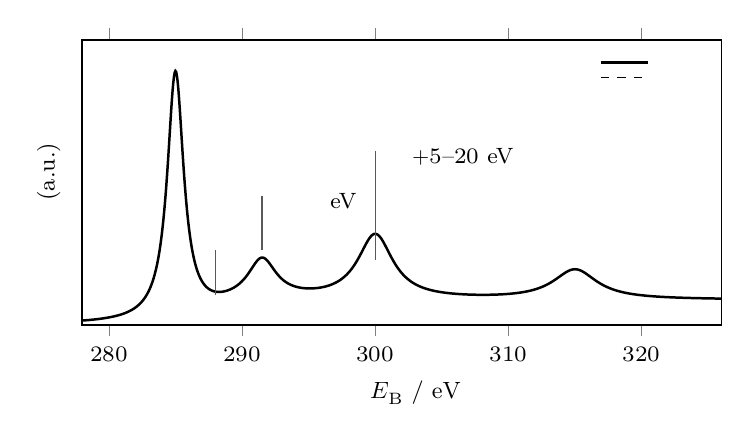
\begin{tikzpicture}
\begin{axis}[
  width=\onecolwidth, height=52mm,
  xlabel={结合能 $E_{\mathrm{B}}$ / \unit{eV}}, ylabel={强度 (a.u.)},
  xmin=278, xmax=326, ymin=0, ymax=1.15,
  xtick={280,290,300,310,320}, ytick=\empty,
  legend pos=north east, legend cell align=left,
  declare function={
    pk(\x,\c,\w,\h)=\h/(1+((\x-\c)/\w)^2);
  }]
% 主峰 + 震激 + 两级等离子激元损失 + 震离台阶（模型计算，非实测）
\addplot[domain=278:326,samples=900,mainline,black]
  {pk(x,285,0.75,1.00)+pk(x,291.5,1.30,0.16)+pk(x,300,1.60,0.26)
   +pk(x,315,2.00,0.12)+0.10*0.5*(1+(x-288)/sqrt((x-288)^2+9))};
% 参考基线
\addplot[domain=278:326,samples=2,thinline,black,dashed]{0};
\legend{模型计算谱,基线}
% 标注
\node[anchor=south,font=\fontsize{8}{9.6}\selectfont] at (axis cs:285,1.02) {主峰};
\draw[thinline,accent] (axis cs:291.5,0.30) -- (axis cs:291.5,0.52);
\node[anchor=west,font=\fontsize{8}{9.6}\selectfont,align=left]
  at (axis cs:292.5,0.52) {震激（卫星）峰\\高结合能侧数 eV};
\draw[thinline,accent] (axis cs:300,0.26) -- (axis cs:300,0.70);
\node[anchor=west,font=\fontsize{8}{9.6}\selectfont,align=left]
  at (axis cs:301,0.70) {等离子激元损失峰\\约 $+5$--$20$ eV，可有多级};
\draw[thinline,accent] (axis cs:288,0.12) -- (axis cs:288,0.30);
\node[anchor=west,font=\fontsize{8}{9.6}\selectfont,align=left]
  at (axis cs:280,0.34) {震离台阶\\连续本底抬高};
\end{axis}
\end{tikzpicture}
\caption{四类伴峰在 XPS 谱上的相对位置。读者应看\textbf{方向}：结合能向右增大，
所以震激峰、等离子激元损失峰都出现在主峰\textbf{右侧}（它们都使出射光电子动能下降）；
震离表现为本底台阶而不是峰；等离子激元损失可以出现多级（间距等距）。
本图为按各过程典型能量间距计算的示意谱，不代表任何具体样品或原书实测图。
\modelmark\figsrc{各类伴峰的相对位置与判据据 S2 §9.2.6（书内 p.617—623 / PDF p.108—114）整理绘制。}}
\label{fig:satellites}
\end{figure}

\subsubsection{震激峰与震离峰}

\textbf{震激（shake up）}是光激发与光电离同时发生的现象：内层电子被光电发射后，
终态弛豫（退激发）导致另一壳层电子被激发到更高能层。它属\textbf{单极激发}——
只有主量子数改变，角量子数与自旋量子数均不变。震激消耗能量，使出射光电子动能下降，
因此震激峰出现在\textbf{主峰高结合能侧、离主线约几个 eV}处。

\textbf{震离（shake off）}是价壳层电子跃迁到非束缚的连续态成为自由电子。它与震激同属
单极激发、同样消耗能量，但在谱图上表现为\textbf{从某个能量开始的连续本底台阶}，
而不是一个峰。震离信号极弱、常被淹没在背底中，实际测试中常被忽略。

\begin{keycond}
震激峰的价值在于\textbf{区分单靠主峰位移区分不了的化学态}。最常被引用的例子是
Cu/CuO/\ce{Cu2O} 体系：用通常的结合能位移区分三者很困难，但它们的 Cu 2p 震激峰
差别明显——\textbf{Cu 和 \ce{Cu2O} 没有明显的 2p$_{3/2}$ 震激峰，而 CuO 有明显的震激峰}。
另一条规律：震激现象在\textbf{顺磁}化合物中发生得很普遍；稀土元素的震激峰强度甚至可以
与主峰相比拟（四价 Ce 的 3d 谱中 3d$_{5/2}$ 与 3d$_{3/2}$ 各有两个震激峰，
且\textbf{震激峰强度超过光电子主峰}）。
\src{S2 §9.2.6，书内 p.618--619 / PDF p.109--110}
\end{keycond}

\subsubsection{X 射线激发的俄歇峰与等离子激元损失峰}

用 \qtyrange{100}{3000}{eV} 的 X 射线源时，绝大多数元素除出射光电子外还出射俄歇电子，
因此 XPS 谱中常伴有俄歇跃迁谱线。俄歇峰的动能同样与化学环境密切相关，
可用其化学位移与峰形变化研究化学态。\textbf{由于俄歇跃迁涉及三电子过程，
其化学位移量往往比光电子峰大得多}——当光电子峰位移不明显时，俄歇峰的位移与峰形
可以提供补充信息。典型例子是 Zn 与 ZnO：Zn 2p 谱较难区分，而 X 射线激发的
Zn LMM 俄歇谱线在峰位与峰形上差别都较大。

\textbf{等离子激元能量损失峰}来自光电子逃逸过程中的非弹性散射。当光电子能量在
\qtyrange{100}{1500}{eV} 时，主要的非弹性散射方式是激发固体中自由电子的集体振荡
（等离子激元）。与一般非弹性散射不同，等离子激元的能量损失是\textbf{特征的、量子化的}。
金属样品通常在光电子峰低动能端 \qtyrange{5}{20}{eV} 处出现主损失峰，并伴随一系列
等间距次级峰；非导体则多表现为一系列长拖尾峰。

\begin{table}[htbp]
\centering
\caption{四类伴峰的来源、位置与用途\src{据 S2 §9.2.6，书内 p.620--622 / PDF p.111--113 归纳。}}
\label{tab:satellite}
{\srcsize
\begin{tabularx}{\columnwidth}{@{}lXX@{}}
\toprule
类型 & 来源与位置 & 读图要点 \\
\midrule
震激（卫星）峰 & 弛豫使另一壳层电子被激发；主峰高结合能侧数 eV & 单极激发；顺磁体系显著；可区分 Cu/\ce{Cu2O}/CuO 类化学态 \\
震离台阶 & 价电子跃迁到连续态；从某能量起本底台阶 & 不是峰而是台阶；信号极弱，常被忽略 \\
俄歇峰 & X 射线激发的三电子过程 & 位移量常大于光电子峰；Zn/ZnO 类体系的关键补充 \\
等离子激元损失 & 逃逸时激发自由电子集体振荡；主峰低动能端 $5$--$20$ eV，可多级 & 金属为等间距尖峰，非导体为长拖尾 \\
\bottomrule
\end{tabularx}}
\end{table}
\emph{核对说明}：已对照原页面图像（书内 p.620--622 / PDF p.111--113）。原书给出：
震激（卫星）峰与震离台阶的区别——震离是价壳层电子跃迁到非束缚的连续状态，从某个能量开始出现连续的较高本底台阶（图
9-64、图 9-65 为示意）；X 射线激发的俄歇跃迁谱线——在 100$\sim$3000 eV 的 X
射线源下绝大部分元素除出射光电子外还出射俄歇电子，俄歇峰的动能也与元素所处的化学环境有密切关系，
其化学位移量往往比光电子峰的更大（图 9-66 为 Zn 与 ZnO 的 Zn 2p 谱及 X 射线激发的 Zn
LMM 俄歇谱，峰位与峰形差别较大）；等离子激元能量损失峰——金属通常在光电子峰的低动能端 5$\sim$20
eV 处观察到主要损失峰，还有一系列次级峰（图 9-67 为金属铝的 2s 光电子峰与一系列的能量损失峰），
而对于非导体通常是一系列长拖尾峰。表中四行均可由这三页支持。

\begin{pitfall}
\textbf{（1）把伴峰当成独立物种。}震激峰与等离子激元损失峰都是同一元素主峰的伴随结构；
若在分峰时把它们当作额外的化学态，会凭空多出并不存在的组分。
判断方法：伴峰与主峰的能量间距是否恒定、是否随激发源改变、是否与主峰强度成比例。
\textbf{（2）分峰时把伴峰面积并入主峰。}反向的错误同样致命：定量时若把震激峰计入主峰面积，
该元素含量会被系统性高估。正确做法是明确交代哪些峰被计入、哪些被排除。
\textbf{（3）忽略等离子激元损失对厚样品的贡献。}损失峰强度随样品厚度增加，
在金属厚膜上可以强到干扰邻近元素的定量。
\end{pitfall}

\begin{crosscheck}
本节的判据都依赖\textbf{参考态实测谱}而非纯理论。若某化学态的归属对结论关键，
应同时给出：（1）参考化合物的实测谱；（2）改变化学态的对照实验（如原位还原/氧化后复测）；
（3）独立手段的交叉验证——表面元素与化学态的整体框架见分片 a，
\textbf{俄歇电子能谱（AES）}的独立介绍见 \chapref{ch:09} 后续分片，
结构层面的对照应用 XRD（\chapref{ch:04}）与化学吸附（\chapref{ch:05}）。
\end{crosscheck}

\srcnote{本分片来源：S2（下册）§9.2.5--§9.2.6，书内 p.615--623 / PDF p.106--114。
式~\eqref{eq:eb-def} 对应原书对 $E_{\mathrm{B}}$ 的定义（OCR 作
「Eb = Ef(n1)Ei(n)」，括号与减号均丢失，按幂次与上下文重建为
$E_f(n-1)-E_i(n)$）。
原书本节所配的实测谱图（图 9-58、9-60—9-68）与震激峰实例均为实验谱，
本书\textbf{未裁切复制}，改以模型计算的示意谱（图~\ref{fig:satellites}）说明相对位置关系；
需要看真实谱形与时例的读者请按上述页码回查原书。
9.2.7—9.2.10（其他初级结构谱线、定量分析、数据后处理、常见问题）由分片 d 续写。}
}{}
\IfFileExists{chapters/parts/ch09-c.tex}{% ================================================================
%  chapters/parts/ch09-c.tex
%  第 9 章 表面分析技术基础（分片 c）
%  源：S2（下册）§9.3–§9.5，书内 p.662—693 / PDF p.153—184
%  覆盖：9.3 UPS、9.4 AES、9.5 ISS
%  承接分片 b（9.2.5–9.2.10 XPS 数据处理与常见问题）
% ================================================================

\subsection{紫外光电子能谱（UPS）}

\begin{probout}
紫外光电子能谱（ultraviolet photoelectron spectroscopy，UPS）测量\textbf{价电子与价带}
的电子结构。它和 XPS 共用同一台谱仪的电子光学系统与分析器，唯一的差别是激发源：
用真空紫外光子（最常用 He I，$h\nu=\qty{21.22}{eV}$）代替 X 射线。
由此带来三个后果：探测深度更浅、能量分辨更高、只能看到价壳层。
因此 UPS 回答的是 XPS 回答不了的那类问题——\textbf{功函数、价带结构、吸附分子的轨道能级}。
\end{probout}

\subsubsection{原理与公式}

UPS 的基本原理与 XPS 相同，仍是 Einstein 光电方程，只是把初态从内层轨道换成价壳层。
对气相分子（原子），能量为 $h\nu$ 的光子电离出一个电子后留下可振动、转动的离子，
出射光电子的动能为

\begin{equation}\label{eq:ups-gas}
E_{\mathrm{K}}=h\nu-I-E_{\mathrm{v}}-E_{\mathrm{r}}
\end{equation}

式中 $I$ 为电离电位（把外层电子从基态激发到无穷远所需能量），$E_{\mathrm{v}}$ 为分子离子
的振动能，$E_{\mathrm{r}}$ 为转动能。$E_{\mathrm{r}}$ 至多只有几个 meV，目前无法测得；
$E_{\mathrm{v}}$ 约 \qtyrange{0.05}{0.5}{eV}，只有高分辨谱仪（分辨能力
\qtyrange{10}{25}{meV}）才能观察到振动精细结构。

对固体表面，忽略平动与转动能，价带电子的能量关系为

\begin{equation}\label{eq:ups-solid}
E_{\mathrm{K}}=h\nu-E_{\mathrm{b}}-\Phi
\end{equation}

式中 $E_{\mathrm{b}}$ 为出射光电子的结合能（相对费米能级），$\Phi$ 为逸出功。
式~\eqref{eq:ups-solid} 是 UPS 测功函数的依据。

\begin{keycond}
式~\eqref{eq:ups-gas} 要求气相、单光子电离且忽略平动转动能；式~\eqref{eq:ups-solid}
要求固体表面\textbf{清洁且导电良好}，并且样品与谱仪之间有明确的费米能级参考。
量纲检查：两式中各项均为能量，习惯以 \unit{eV} 计。$h\nu$ 由光源线型决定，
He I $\alpha$ 为 \qty{21.22}{eV}，是功函数与价带测量的常用工作点。
\end{keycond}

\begin{example}[用 UPS 测 Au 的功函数（教学设定数值）]
实验采用 He I 共振线，$h\nu=\qty{21.2}{eV}$。谱图上取费米边为 $E_{\mathrm{Fermi}}=0$，
二次电子截止边为 $E_{\mathrm{cutoff}}=\qty{16.1}{eV}$。因截止边对应动能为零的光电子，
有 $\Phi=h\nu-E_{\mathrm{cutoff}}=\qty{21.2}{eV}-\qty{16.1}{eV}=\qty{5.1}{eV}$，
与金的公认功函数一致。\pedset{本算例按 S2 §9.3.3（书内 p.669 / PDF p.160）的实测数字整理，
但请以原文为准；仪器需施加约 \qty{-5}{V} 的负偏压以使截止边落入分析器能量窗口。}
\end{example}

\subsubsection{与 XPS 的分工}

表~\ref{tab:ups-xps} 是本节最该记住的内容：UPS 与 XPS 不是替代关系，而是分工关系。

\begin{table}[htbp]
\centering
\caption{UPS 与 XPS 的分工\src{据 S2 §9.3.1--§9.3.4，书内 p.662--670 / PDF p.153--161 归纳。}}
\label{tab:ups-xps}
{\srcsize
\begin{tabularx}{\columnwidth}{@{}lXX@{}}
\toprule
对比项 & UPS & XPS \\
\midrule
激发源 & 真空紫外（He I \qty{21.22}{eV}） & X 射线（Al K$\alpha$ \qty{1486.6}{eV}） \\
本征线宽 & 约 \qty{0.01}{eV}，单色化可达 \qty{1}{meV} & 约 \qty{0.5}{eV} 量级 \\
探测对象 & 价电子、价带、表面态 & 内层电子 \\
信息深度 & 约 10 个原子层 & 约 30 个原子层 \\
价带谱质量 & 强度与分辨均优于 XPS & 可用但分辨较差 \\
化学位移 & 峰宽、不易精确测，多为峰形变化 & 内层化学位移明确，是主用途 \\
能否分辨振动结构 & 能（\qty{0.05}{eV}），单色化后甚至可分辨转动 & 不能（内层结合能远高于振转能，且源线宽过宽） \\
谱解释难度 & 较难，严谨解释需分子轨道计算 & 相对直接 \\
\bottomrule
\end{tabularx}}
\end{table}

\begin{pitfall}
\textbf{（1）「UPS 也能测化学态」是误解。}UPS 涉及成键轨道，电子属于整个分子，
谱峰宽，不易精确测化学位移，一般只能靠峰形变化判别。判断化学态仍应以 XPS 为主。
\textbf{（2）UPS 的信息深度更浅，因此对污染更敏感。}表面污染物（碳、氧）的价电子
谱线会直接叠在待测价带上。未做氩离子刻蚀清洁的 Au 价带谱，费米边与轨道能级
根本分不清。
\textbf{（3）绝缘样品特别是粉末不适合 UPS。}粉末表面存在无法去除的污染层，
且荷电无法有效中和。
\textbf{（4）谱图不直接等于态密度。}固体表面测得的光电子能量分布不直接代表状态分布，
需要通过简化模型计算才能与态密度对应。
\end{pitfall}

\begin{measure}
UPS 实验要点：分析室真空度应优于 \qty{1e-9}{mbar}；选择合适负偏压（一般约
\qty{-5}{V}）以观测截止边；气源纯度优于 $99.999\%$ 且气路短、无泄漏；
UV 束斑达 \unit{mm} 级，故样品不宜过小；导电样品与样品台须良好接地；
还需考虑 UV 对样品表面的副效应。
\src{S2 §9.3.5，书内 p.670--671 / PDF p.161--162}
\end{measure}

\subsection{俄歇电子能谱（AES）}

\begin{probout}
俄歇电子能谱（Auger electron spectroscopy，AES）用电子束激发，探测\textbf{俄歇电子}。
最关键的性质是：\textbf{俄歇电子的能量只由原子的能级结构决定，与激发源的能量和种类无关。}
这一性质使 AES 既能在固定能量处识别元素，又能用电子束聚焦获得很高的空间分辨率，
因而特别适合微区分析与薄膜、器件的失效分析。它是目前应用广度仅次于 XPS 的表面分析方法。
\end{probout}

\subsubsection{原理}

俄歇过程涉及三个电子：入射粒子（光子、电子或离子）击出内层电子形成空穴；
外层电子向空穴跃迁并释放能量；该能量以非辐射方式激发另一个电子（即俄歇电子）逃逸。
因为能量来自原子自身的能级差，所以俄歇峰的位置\textbf{不随激发源改变}——
这正是 AES 可以做成扫描微区成分分析的基础。

\begin{keycond}
俄歇电子能量在 \unit{keV} 量级，衰减长度很短，只有前几个原子层
（约 2--10 层）产生的俄歇电子能逃逸出来。因此 AES 比 XPS 更表面敏感，
但也意味着\textbf{任何表面污染都会强烈影响结果}。AES 通常只适用于导电与半导电样品，
绝缘样品必须先解决荷电问题。
\end{keycond}

\subsubsection{定量与校准}

AES 定量采用相对灵敏度因子法：

\begin{equation}\label{eq:aes-quant}
x_{\mathrm{A}}=\frac{I_{\mathrm{A}}/s_{\mathrm{A}}}{\sum_{i} I_{i}/s_{i}}
\end{equation}

式中 $x_{\mathrm{A}}$ 为元素 A 的原子分数，$I_{\mathrm{A}}$ 为 A 的 AES 强度，
$s_{\mathrm{A}}$ 为 A 的相对灵敏度因子。由于俄歇峰（直接谱）较宽，实测中一般取
\textbf{微分谱的峰对峰高度}作为峰强度。

\begin{pitfall}
\textbf{（1）灵敏度因子随激发能量而变。}电子束能量 3 keV 与 5 keV 下，
各俄歇跃迁的相对灵敏度因子分布不同，引用时必须说明激发条件，
不能跨仪器、跨束能直接比强度。
\textbf{（2）能量标尺必须校准。}早期用 Au MNN = \qty{2024}{eV}、
Ag MNN = \qty{356}{eV}、Cu LMM = \qty{920}{eV} 三点校准；
现行做法依 ISO 标准：ISO 17973（中等分辨率 AES 能量标尺校准，用于元素分析）、
ISO 17974（高分辨率 AES，用于元素与化学态）、ISO 21270（XPS 与 AES 强度标的线性）、
ISO 24236（AES 强度标的重复性与稳定性）。
\textbf{（3）重元素谱线重叠严重。}轻元素俄歇跃迁少、易识别；重元素跃迁多、易干扰。
例如 Cr 至 Cu 的 LMM 跃迁相互重叠，而这恰是钢铁材料 AES 分析的关键位置。
必须事先确认峰位不重叠，并与标准谱图对照。
\textbf{（4）绝缘样品的处理是硬约束。}可把小绝缘颗粒镶嵌在纯软金属箔（铟、铝）中、
表面加盖金属导电筛网使电子束穿孔通过、减薄样品降低绝缘性，
或用低能正离子中和表面负电荷；无论哪种，导电层都须良好接地。
\end{pitfall}

\subsection{离子散射谱（ISS）}

\begin{probout}
离子散射谱（ion scattering spectroscopy，ISS）测量\textbf{一定能量的离子在表面原子上
弹性散射后的能量}。它探测的是\textbf{最外层原子}，是本书介绍的四类表面方法中
信息深度最浅的一个，因而对「表面最外层到底由什么原子终止」这类问题最直接。
一般多功能电子能谱仪配的是低能离子散射（LEISS，离子动能 \qtyrange{200}{3000}{eV}）；
按能量还分为 MEISS（中能）与 HEIS／RBS（高能，卢瑟福背散射）。
\end{probout}

\subsubsection{原理与公式}

已知质量 $m_1$、能量 $E_0$ 的一次离子轰击表面原子（质量 $m_2$），在固定散射角 $\theta$
处测量弹性散射后的一次离子能量 $E_1$，由能量与动量守恒得

\begin{equation}\label{eq:iss-ch09}
\frac{E_1}{E_0}=\left[\frac{\cos\theta\pm\sqrt{(m_2/m_1)^2-\sin^2\theta}}{1+m_2/m_1}\right]^{2}
\end{equation}

\begin{keycond}
式~\eqref{eq:iss-ch09} 成立的前提是\textbf{单次二元弹性碰撞}（表面足够稀薄、无多重散射）
且忽略靶原子反冲的能量损失以外的过程。极限情况检查：当 $\theta=90^{\circ}$ 时
$\cos\theta=0$，取正号分支化简得
$E_1/E_0=(m_2-m_1)/(m_2+m_1)$，与二元碰撞的标准结果一致，
可作为公式与符号约定的自检。由式可知：测得 $E_1/E_0$ 即可反推 $m_2$（识别元素），
而峰高比可用于推断表面原子的排列与覆盖——这正是 ISS 兼具成分与结构信息的原因。
\end{keycond}

\begin{pitfall}
\textbf{（1）ISS 只看到最外层。}这既是优点也是局限：它无法给出亚表面层的成分，
要获得深度信息必须配合离子溅射做深度剖析，而溅射本身会破坏表面。
\textbf{（2）离子轰击会造成表面损伤与择优溅射。}轻元素优先被溅射，
长时间测量会使表面组成偏离真实值。
\textbf{（3）定量比 XPS/AES 更困难。}散射截面、中和概率与表面几何都影响峰高，
一般只做半定量或相对比较。
\end{pitfall}

\subsection{四种表面方法的比较与选择}

把本章四类方法放在一起看，选择的依据不是「哪个更好」，而是
\textbf{你要的是内层化学态、价带结构、微区成分，还是最外层组成}（表~\ref{tab:surface-compare}）。

\begin{table}[tbp]
\centering
\caption{四类表面分析方法的比较。信息深度一栏决定了「表面」在此处的实际含义\src{据 S2 §9.3--§9.5，书内 p.662--693 / PDF p.153--184 归纳。}}
\label{tab:surface-compare}
{\srcsize
\begin{tabularx}{\twocolwidth}{@{}p{16mm}p{26mm}p{20mm}p{16mm}p{30mm}X@{}}
\toprule
方法 & 探测信号 & 激发源 & 信息深度 & 主要信息 & 主要局限 \\
\midrule
XPS & 光电子（内层） & X 射线 & 约 3--10 nm & 元素组成、化学态、半定量 & 空间分辨较低；荷电与污染影响大；分峰非唯一 \\
UPS & 光电子（价带） & 真空紫外 & 约 1--3 nm（约 10 原子层） & 功函数、价带结构、吸附分子轨道 & 需极洁净表面；绝缘粉末不适用；谱解释难 \\
AES & 俄歇电子 & 电子束 & 约 0.5--2 nm（2--10 原子层） & 轻元素与微区成分、深度剖析 & 重元素谱线重叠；仅导电/半导电样品；束损伤 \\
ISS & 散射离子 & 惰性气体离子 & 最外层原子 & 表面最外层组成与排列 & 仅最外层；离子损伤与择优溅射；定量难 \\
\bottomrule
\end{tabularx}}
\end{table}

\begin{dataflow}
选择顺序：（1）要\textbf{化学态}、且样品可承受 X 射线 → XPS；（2）要\textbf{功函数或
价带}（如金属-载体相互作用、半导体界面） → UPS，且必须先确认表面洁净；
（3）要\textbf{微区}或\textbf{深度剖面}（器件、薄膜、失效分析） → AES；
（4）只关心\textbf{最外层由什么原子终止} → ISS。若三者都需要，
现代多功能谱仪通常可在同一超高真空系统中完成，避免样品在转移中被污染——
\textbf{这是联合使用这三类方法最重要的实际理由}。
\end{dataflow}

\begin{crosscheck}
本章的 XPS 数据处理与常见问题见分片 b；表面分析在催化中的具体应用与准原位技术、
近常压 XPS 见分片 d。若关心的是\textbf{表面吸附物种与反应中间物}而非表面元素组成，
应转向原位振动光谱（\chapref{ch:06}、\chapref{ch:07}）与化学吸附/程序升温技术
（\chapref{ch:05}）——表面分析给出的是「有什么原子」，不是「在怎样反应」。
\end{crosscheck}

\srcnote{本分片来源：S2（下册）§9.3--§9.5，书内 p.662--693 / PDF p.153--184。
式~\eqref{eq:ups-gas}、\eqref{eq:ups-solid} 对应原书式(9-11)、(9-12)，
式~\eqref{eq:aes-quant} 对应式(9-15)，式~\eqref{eq:iss-ch09} 对应式(9-16)；
四式均由「OCR 正文的变量定义 + 学科标准形式」重建，
其中式~\eqref{eq:iss-ch09} 已用 $\theta=90^{\circ}$ 的极限结果做过自检。
原书表格（惰性气体光子能量表 9-23、He 辐射线型表 9-24、AES 灵敏度因子图 9-136、
Cr--Cu 俄歇跃迁谱图 9-137 等）未逐表转录，
需要的读者请按上述页码回查原书。}
}{}
\IfFileExists{chapters/parts/ch09-d.tex}{% =====================================================================
% 第 9 章 表面分析技术基础  分片 d
% 覆盖：§9.2.7 其他初级结构谱线 / §9.2.8 定量（半定量）分析
%       §9.2.9 数据后期处理 / §9.2.10 实验中的常见问题
% 注意：源文件 ch09-d.txt 的实际节号为 §9.5 尾＋§9.6—§9.8；§9.2.7—§9.2.10 的原书正文见书内 p.623—641，其 OCR 在 sources/parts/ch09-b.txt。逐条核对结果见各节「核对说明」。
% =====================================================================

\subsection{XPS 中除芯能级谱外的其他初级结构谱线的应用}
\label{sec:ch09-otherlines}

\emph{核对说明}：本节材料已对照原页面图像（书内 p.705—708 / PDF p.196—199）。价带谱材料在源文件 §9.6.2「参考 C 的价带谱」（书内 p.705—706）：PBMA（聚甲基丙烯酸正丁酯）的三个同分异构体 C 1s 峰型与峰位一致（图 9-156a），而价带谱差异明显（图 9-156 b、c、d）；聚烯烃 PE、PP、PB、PIB、PI 与 PS 的 C 1s 谱也难区分，价带谱有差别（图 9-157，书内 p.706）。shake-up 材料在同节「C 1s 的 Shake-up 峰分析」（书内 p.706—708）：石墨与碳纳米管的 C 1s 均为 284.6 eV、\ce{C60} 为 284.75 eV（书内 p.707），\ce{C60} 的 shake-up 峰可分解为 5 个峰（书内 p.708）。需要说明的是：§9.2.7—§9.2.10 的原书正文确实存在，其 OCR 文本落在另一分片的源文件 \texttt{sources/parts/ch09-b.txt}（§9.2.7 起于第 227 行，§9.2.8 起于第 415 行／书内 p.630，§9.2.9 起于第 589 行／书内 p.633，§9.2.10 起于第 780 行／书内 p.640），本分片的源文件 \texttt{ch09-d.txt} 并不覆盖这四节（其实际内容为 §9.5 末＋§9.6—§9.8，书内 p.694—733 / PDF p.185—224）。本分片各节按任务书的节号编排，正文为按学科标准形式的改写，逐条核对结果见各节前的核对说明。

\begin{probout}
芯能级主峰回答的是"有什么元素、各元素处在什么化学态、相对量多少"三件事。除此之外还有三类初级结构谱线能回答主峰回答不了的问题：\emph{价带谱}回答成键与电子结构（同分异构体、同类聚合物的区分）；\emph{shake-up 与 shake-off 伴峰}回答未占据态与共轭程度（石墨碳、碳纳米管与 \ce{C60} 的鉴别）；\emph{X 射线激发 Auger 谱（XAES）与 Auger 参数}回答化学态，并且能在很大程度上抵消荷电漂移。
\end{probout}

\begin{principle}
震激（shake-up）与震离（shake-off）的机理已在「终态效应及伴峰」一节（§~\ref{sec:ch09-satellites}）给出，这里只讲它们的\emph{应用}：$\pi\to\pi^{*}$ 震激峰与共轭程度直接相关，是石墨碳、碳纳米管与 \ce{C60} 的鉴别依据；震离则形成宽而弱的背景结构。价带谱是价电子态密度经各轨道光电离截面加权后的分布，出现在约 $0\sim30$ eV 的低结合能区。

X 射线激发的 Auger 电子动能由三个能级之差决定，与激发光子能量无关；把同一元素的 Auger 动能与光电子结合能相加，得到 Wagner 修饰 Auger 参数
\begin{equation}
\alpha' = E_{\mathrm{K}}(\text{Auger}) + E_{\mathrm{B}}(\text{光电子})
\label{eq:ch09-augerparam}
\end{equation}
样品荷电使 $E_{\mathrm{B}}$ 增加 $q$、使 Auger 动能减少 $q$，两者在 $\alpha'$ 中一阶抵消，因此 $\alpha'$ 对荷电不敏感，可用于区分化学态并跨仪器比较。
\emph{核对说明}：已对照原页面图像（书内 p.625 / PDF p.116）。原书印：$\alpha = \mathrm{EK_A} - \mathrm{EB_P}$（式 9-6）、$\alpha' = \alpha + h\nu = \mathrm{EK_A} + \mathrm{EB_P}$（式 9-7），式中 $\mathrm{EB_P}$ 为最强光电子线的结合能、$\mathrm{EK_A}$ 为最尖锐俄歇线的动能，并给出 Wagner 图与部分 Cu 化合物的 Cu 2p／Cu L$_3$VV 参考峰位及 $\alpha'$ 参考值（图 9-71）。故本式 $\alpha' = E_{\mathrm{K}}(\text{Auger}) + E_{\mathrm{B}}(\text{光电子})$ 并非无据重建：它与原书式 (9-7) 形式一致，仅符号写法不同（原书用 $\mathrm{EK_A}$／$\mathrm{EB_P}$，本分片用 $E_{\mathrm{K}}$／$E_{\mathrm{B}}$），判定为形式一致但符号不同；式前「样品荷电使 $E_{\mathrm{B}}$ 增加 $q$、Auger 动能减少 $q$ 而一阶抵消」的补偿关系为按学科标准形式的补充说明，原书未展开。
\end{principle}

\begin{measure}
价带谱：低通能（约 20—50 eV）、小步长（$\le0.1$ eV）、长驻留；用单色 Al K$\alpha$ 可去掉 K$\alpha_{3,4}$ 卫星线（它会在主峰高结合能约 9.8 eV 处造出一个假伴峰）。样品必须与样品台电接触良好，否则费米边畸变会被误读成"带隙变化"。伴峰测量仍用常规高分辨窄扫，但需要长采集才能取得主峰强度 $10^{-2}$ 量级的弱结构，同时必须把 X 射线累积剂量控制在损伤阈值以下（见 §\ref{sec:ch09-problems}）。
\end{measure}

\begin{dataflow}
价带谱或伴峰 $\to$ 与标准谱／态密度计算对照 $\to$ 成键与共轭判断 $\to$ 与同一批样品的芯能级化学态结论联合 $\to$ 结构归属。任何一步缺失（只有谱而没有对照，或没有芯能级支持），结论只能写成"与……一致"，不能写成"证明是……"。
\end{dataflow}

\paragraph{读谱实例：主峰分不开的碳材料，靠伴峰分开}
\begin{obs}
石墨与碳纳米管的 C 1s 主峰都在 284.6 eV（差别小于 0.15 eV，常规分辨率下不可分辨）；两者在主峰高结合能侧约 6—7 eV 处都有 $\pi$-$\pi^{*}$ 伴峰；\ce{C60} 的 C 1s 为 284.75 eV，其伴峰区域更宽，可分解为 5 个成分。同类证据来自 PBMA 的三个同分异构体：C 1s 峰型与峰位一致，而价带谱差异明显；聚烯烃 PE、PP、PB、PIB、PI 与 PS 的 C 1s 也难区分，而价带谱有别。\src{源文件 §9.6.2，书内 p.705—708 / PDF p.196—199}
\end{obs}
\begin{infer}
石墨与碳纳米管的伴峰结构一致 $\Rightarrow$ 两者价电子结构相近，碳原子均以 sp$^{2}$ 杂化形成共轭 $\pi$ 键，可归为一类；\ce{C60} 的伴峰含额外成分 $\Rightarrow$ 除共轭 $\pi$ 键外还有明显的 $\sigma$ 键贡献，须单独归属。\emph{注意}：这里推断的是"电子结构相近／不同"，不是"结构相同"；把价带谱与伴峰当指纹使用前需要大量标准谱储备，目前这类应用总体上仍停留在指纹水平，还需理论计算支撑。
\end{infer}

\begin{pitfall}
（1）把 shake-up 伴峰当作一个新的化学态单独定量——伴峰是主峰的卫星，其强度已包含在主峰的归属里，重复计入会使该元素的原子分数偏高。（2）把 Al K$\alpha_{3,4}$ 卫星线当成伴峰，或把 Mg K$\alpha$ 源下约 8—10 eV 处的卫星结构误读为共轭特征。（3）用价带谱直接断言骨架结构而不做对照与计算。（4）在绝缘粉末上测价带谱并用费米边定标。（5）样品已被 X 射线损伤（脱氟、氧化、交联）之后，再把伴峰结构的变化当作本征信息。
\end{pitfall}

\begin{crosscheck}
价带谱与 UPS（He I，21.2 eV）对照：UPS 分辨率更高、价带精细结构更清楚，而 XPS 价带谱可与同批样品的芯能级在同一次装样中测得，条件一致性更容易保证。化学态归属用 Auger 参数与 XANES／EXAFS 回查；聚合物骨架用 IR／Raman 与固体 NMR 回查；碳材料用 Raman（D 带／G 带）回查。
\end{crosscheck}

\subsection{XPS 定量（半定量）分析}
\label{sec:ch09-quant}

\emph{核对说明}：本节有原书对应正文，已对照原页面图像（书内 p.630、p.632—p.633 / PDF p.121、p.123—p.124）并通查其 OCR 全文（\texttt{sources/parts/ch09-b.txt} 第 415—588 行，即原书 §9.2.8「XPS 定量（半定量）分析」，书内 p.630 起）。原书给出的关键式：式 (9-8) $I_{ij} = K\,T(\mathrm{KE})\,L_{ij}(\gamma)\,\sigma_{ij}\!\int n_i(z)\mathrm{e}^{-z/(\lambda(\mathrm{KE})\cos\theta)}\,\mathrm{d}z$、式 (9-9) $n_i/n_j = (I_i/S_i)/(I_j/S_j)$、式 (9-10) $n_i/n_j = (I_i/I_j)(\sigma_j/\sigma_i)(\mathrm{EK}_j^{0.5}/\mathrm{EK}_i^{0.5})$，并强调「XPS 的真正定量分析很难……给出的常常是一种半定量的分析结果」，报出的是相对原子分数而不是质量分数。本节正文为按学科标准形式的改写：式 \equref{eq:ch09-quant-int}、\equref{eq:ch09-rsf}、\equref{eq:ch09-atomfrac} 与原书上式形式一致而符号与因子取舍不同（本节把式 (9-8) 的深度积分简化为 $\lambda_i\cos\theta$ 因子、按原书「对固体通常被忽略」略去 $L_{ij}(\gamma)$，并显式写出探测效率 $D(E_i)$），判定为形式一致但符号不同，并属改编补充。

\begin{probout}
XPS 定量能得到的是\emph{采样深度内}（约 $3\lambda\cos\theta$，常规为几纳米到十几纳米）元素的\emph{相对}原子分数、表面富集或偏析程度、活性组分的表面浓度。它得不到体相组成，也得不到绝对含量（除非对同基体标样做工作曲线）。因此本书与仪器厂商一致地把 XPS 定量称为\emph{半定量}。
\end{probout}

\begin{principle}
第 $i$ 个元素某芯能级的信号强度可以写成
\begin{equation}
I_i \;\propto\; n_i\,\sigma_i(h\nu)\,\lambda_i(E_i)\,T(E_i)\,D(E_i)\cos\theta
\label{eq:ch09-quant-int}
\end{equation}
其中 $n_i$ 为原子体密度，$\sigma_i$ 为该能级在光子能量 $h\nu$ 下的光电离截面，$\lambda_i$ 为电子在该基体中的非弹性平均自由程，$T(E_i)$ 为分析器透射函数，$D(E_i)$ 为探测器效率，$\theta$ 为相对表面法线的取出角，$E_i = h\nu - E_{\mathrm{B},i} - \varphi_{\mathrm{sp}}$ 为光电子动能。把与基体和仪器有关的因子归并成\emph{相对灵敏度因子}
\begin{equation}
S_i \;\propto\; \sigma_i(h\nu)\,\lambda_i(E_i)\,T(E_i)\,D(E_i)
\label{eq:ch09-rsf}
\end{equation}
则峰面积 $A_i \propto I_i$，原子分数为
\begin{equation}
C_i = \frac{A_i/S_i}{\sum_j A_j/S_j}
\label{eq:ch09-atomfrac}
\end{equation}
这就是灵敏度因子法。$\lambda$ 随动能缓慢增加（约 $E^{0.5\sim0.8}$；Seah--Dench 经验式给出以单层数表示的 $\lambda \approx 538E^{-2}+0.41a^{3/2}E^{1/2}$，$E$ 为动能／eV，$a$ 为单层厚度／nm），因此同一元素的不同谱线、不同元素之间的采样深度并不相同。
\emph{核对说明}：已对照原页面图像（书内 p.630、p.633 / PDF p.121、p.124）。原书给出式 (9-8)（含 $K\,T(\mathrm{KE})\,L_{ij}(\gamma)\,\sigma_{ij}$ 与深度积分）与半定量近似式 (9-10)（含 $\mathrm{EK}^{0.5}$），并说明单质材料在 100—2000 eV 间 $\lambda$ 近似正比于 $\mathrm{EK}^{0.5}$；本节的 $I_i \propto n_i\sigma_i\lambda_i T_i D_i\cos\theta$、$S_i$ 归并式与 $C_i$ 归一式为按学科标准形式的改写，与原书式 (9-8)、(9-9) 形式一致而符号与取舍不同。Seah--Dench 经验式及其常数（538、0.41）属原书未给出：原书 §9.2.5—§9.2.10 的 OCR 全文（\texttt{ch09-b.txt}）中未出现该式，Seah--Dench 仅见于本分片文末参考文献 [10]（书内 p.732 / PDF p.223），正文并未引用，故常数与「$E^{0.5\sim0.8}$」一并记为本改编本按通用文献补入。
\end{principle}

\begin{measure}
半定量的可靠性几乎完全由"条件一致性"决定：同一批样品、同一天、同一 X 射线源与功率、同一通能（透射函数 $T(E)$ 随通能变化）、同一步长与驻留时间、同一取出角。定量必须用高分辨窄扫描，宽扫描只用于元素识别。样品要压成平整致密的片——粉末直接撒在胶带上会同时引入粗糙阴影与胶带污染。记录样品是否含氢：XPS 测不到 H，报出的 at\% 是"除 H 外归一"的结果，与 XRF／ICP 的质量分数不可直接比较。
\end{measure}

\begin{dataflow}
窄扫谱 $\to$ 能量校准 $\to$ 背景扣除 $\to$ 分峰定面积 $\to$ 灵敏度因子归一（式 \equref{eq:ch09-atomfrac}）$\to$ 原子分数 $\to$ 与体相技术比较 $\to$ 结论。每一步都要能报出不确定度：面积拟合误差、灵敏度因子不确定度、背景模型带来的系统偏差。
\end{dataflow}

\paragraph{为什么只能算半定量：四类不可消除的偏差}
\begin{itemize}
\item \textbf{基体效应}。灵敏度因子通常在特定标样、特定仪器条件下测得，$\sigma$、$\lambda$、$T$ 都与基体密度、电子结构、带隙以及仪器透镜模式与通能有关；文献中的灵敏度因子不能跨仪器直接搬用，同一台仪器改变通能，$T(E)$ 曲线改变，定量结果也随之变化。
\item \textbf{逃逸深度差异}。Al K$\alpha$ 下 C 1s（动能约 1200 eV）的 $\lambda$ 约 2—3 nm，而 Ni 2p（动能约 630 eV）只有约 1.0—1.5 nm。表面存在成分梯度（偏析、钝化层、碳覆盖层、载体包覆）时，各元素的"原子比"实际来自不同深度；改变取出角该比值就会变，说明它不是一个体相量。
\item \textbf{样品不均匀}。粉末、粗糙表面、多孔载体、岛状分布的活性组分都会破坏式 \equref{eq:ch09-quant-int} 中的 $\cos\theta$ 假设（阴影、遮蔽、孔壁再吸收），表观浓度一般偏低；活性组分以颗粒存在时，颗粒内部信号被自身衰减，会进一步低估。
\item \textbf{污染层}。吸附碳氢层与水／氧化层使出射电子按 $\exp[-d/(\lambda\cos\theta)]$ 衰减；动能低的谱线衰减更重，因此表面金属组分（Ni 2p、Co 2p、Fe 2p）比污染碳（C 1s，动能高）被压得更低，表观金属含量系统性偏低。污染层厚度随抽真空时间与样品历史变化，同一个"原子比"在一天之内就可能漂移。
\end{itemize}
此外还有三个放大误差的来源：化学态改变会改变峰形与有效截面；卫星峰与多重分裂若归类不当会使面积失真；峰重叠（如 Ru 3d$_{5/2}$ 与 C 1s、Sb 3d$_{5/2}$ 与 O 1s）必须先分峰再报数。

\paragraph{检出限与误差怎么报}
常规条件下 XPS 的检出限约为 0.1—1 at\%（均匀样品、强谱线、充分累加计数）；轻元素与弱谱线更差。低于检出限的结果只能写成"未检出（$<$检出限）"。误差报告的通行做法：\emph{同批样品之间比较}取 $\pm5\%\sim\pm10\%$；\emph{绝对原子分数}（跨仪器、跨实验室）取 $\pm20\%\sim\pm30\%$。并且必须同时写明三件事：是否把污染碳计入总量、是否做过深度或取出角修正、检出限是多少。

\paragraph{读谱实例：一个表面 Ni 含量被污染层压低的算例}
\begin{obs}
同一条件下的窄扫面积（示意值，计数$\cdot$eV）：$A(\mathrm{C\ 1s})=2.0\times10^{4}$，$A(\mathrm{O\ 1s})=4.0\times10^{4}$，$A(\mathrm{Ni\ 2p_{3/2}})=1.2\times10^{3}$。取相对灵敏度因子 $S(\mathrm{C\ 1s})=0.25$、$S(\mathrm{O\ 1s})=0.66$、$S(\mathrm{Ni\ 2p_{3/2}})=4.2$（相对 F 1s 的量级值），按式 \equref{eq:ch09-atomfrac} 归一得 C $\approx$ 57 at\%，O $\approx$ 43 at\%，Ni $\approx$ 0.2 at\%。
\emph{核对说明}：已对照原页面图像（书内 p.632—p.633 / PDF p.123—p.124）。原书印有两套灵敏度因子：表 9-14 为 Scofield 计算的理论元素灵敏度因子（基于 C 1s $=1$，用时须增加分析深度项 $\lambda$，通常取 $\mathrm{KE}^{0.6}$），表 9-15 为由 PHI 谱仪公司提供的实验灵敏度因子（基于 F 1s $=1$，须按分析器类型——半球形或筒镜形——乘峰动能修正），并写明「一般使用元素灵敏度因子法准确度优于 15\%，在同一仪器上使用标准样品测量准确度优于 5\%」。本节算例的 $S(\mathrm{C\ 1s})=0.25$、$S(\mathrm{O\ 1s})=0.66$、$S(\mathrm{Ni\ 2p_{3/2}})=4.2$ 与表 9-15 同以 F 1s 为基准，量级一致，但未逐值照抄原书表（页面图像分辨率不足以保证逐值读取），属按通用文献量级取的示意值；按式 \equref{eq:ch09-atomfrac} 复算 $A/S$ 依次为 $8.0\times10^{4}$、$6.06\times10^{4}$、$2.86\times10^{2}$，归一后 C $\approx57$ at\%、O $\approx43$ at\%、Ni $\approx0.20$ at\%，与本例所报数值自洽。实际报数须改用本台仪器、本通能下测得的灵敏度因子。
\end{obs}
\begin{infer}
不能由 0.2 at\% 直接推断"Ni 流失或分散度极低"：若表面存在约 2 nm 的碳质污染层，Ni 2p（动能约 630 eV，$\lambda\approx1.3$ nm）的衰减因子约 0.2，而 C 1s 与 O 1s（$\lambda\approx2.5$—3 nm）约 0.5，表观 Ni 分数会被压低约 2—3 倍。另外 0.2 at\% 已接近检出限，相对不确定度很大。\emph{处置}：用 \ce{Ar+} 轻刻蚀（注意择优溅射与离子束还原）或在较大取出角下复测，报数时注明"含污染层、未做深度修正"。
\end{infer}

\begin{pitfall}
（1）把 at\% 当准确值，不报误差、不报检出限（见 §\ref{sec:ch09-problems}）。（2）直接引用文献灵敏度因子而不核对仪器与通能。（3）把污染碳计入组成，据此讨论"积炭"或"碳覆盖度"——必须先证明那部分碳属于样品（峰形、结合能、$\pi$-$\pi^{*}$ 伴峰、刻蚀前后对比）。（4）用动能相差很大的两根谱线比较"表面"与"体相"而不考虑 $\lambda$ 差异。（5）把 \ce{Ar+} 刻蚀后的定量结果当作原始表面：择优溅射与离子束诱导的还原、偏析都会改变表层组成。（6）把灵敏度因子归一后的表面浓度直接与催化活性关联，而不先证明该表面物种就是活性位。
\end{pitfall}

\begin{crosscheck}
体相组成用 XRF／ICP-AES 回查；最表层（单原子层）组成用 LEIS 与 RBS 回查；微区组成用 EDS／WDS 回查（采样深度在微米量级，与 XPS 的纳米量级恰好互补）。在同一台仪器上用同基体标样做工作曲线，可以把半定量提升为"带标样的定量"。
\end{crosscheck}

\subsection{XPS 数据的后期处理}
\label{sec:ch09-postproc}

\emph{核对说明}：本节有原书对应正文，已对照原页面图像（书内 p.633—p.635 / PDF p.124—p.126）并通查其 OCR 全文（\texttt{sources/parts/ch09-b.txt} 第 589—779 行，即原书 §9.2.9「XPS 数据的后期处理」，书内 p.633 起）。原书按「1. 荷电校正／2. 使用非单色化激发源，需进行卫星峰扣除／3. 光电子峰的识别，定性分析／4. 适度的谱线平滑处理／5. 本底扣除（线性与非线性两种；shirley 本底、smart 本底、tougaard 本底）」的顺序列出，并对本底成因（非弹性散射电子与次级电子在光电子谱峰的高结合能侧形成本底，轫致辐射本底随光电子动能降低而增强）与 shirley 本底的定义作了文字说明，但全节未给出任何背景扣除公式。本节正文（含式 \equref{eq:ch09-shirley}、\equref{eq:ch09-tougaard} 与分峰约束）为按学科标准形式的改写：方法分类与原书一致，公式、符号与分峰约束属改编补充（原书未印）。

\begin{probout}
后处理只回答三个问题：能量标尺可信吗（荷电校准）；峰下面的背景怎么去掉（面积才可比）；峰能拆成几个化学态、这个拆法唯一吗（背景模型、线型约束与不确定度）。这三步中任何一步没有交代清楚，后面报出的"化学态比例"都无法复核。
\end{probout}

\begin{principle}
\textbf{背景的物理来源}\quad 光电子在逸出途中发生非弹性散射，损失能量后落到主峰\emph{高结合能侧}，形成阶跃状背景；叠加的二次电子级联则给出随结合能缓慢上升的宽背景。所以 XPS 谱的背景总是"往高结合能方向抬升"。

\textbf{线性背景}\quad 取峰两侧平坦区的两点连成直线，假设峰区背景近似线性。算法最简单、结果可复现，适合窄能区、背景平坦、两端有明确平坦区的场合；它的风险是把台阶状背景当成直线，在台阶明显时系统性过扣高结合能一侧。

\textbf{Shirley 背景}\quad 假设任一点处的非弹性背景正比于该点\emph{低结合能侧}已经积累的峰强度（即所有可能在此处贡献损失电子的源），迭代求解：
\begin{equation}
B^{(n+1)}(x) = k\int_{x_0}^{x}\bigl[\,I(x')-B^{(n)}(x')\,\bigr]\,\mathrm{d}x'
\label{eq:ch09-shirley}
\end{equation}
其中 $k$ 由两端点的背景取值确定。它对台阶状背景的适应性最好，是目前最常用的做法；代价是结果依赖端点选择、需要迭代收敛（有时不收敛），而且它本身不带物理参数，不能用来反推损失函数。

\textbf{Tougaard 背景}\quad 用电子非弹性散射的普适截面 $K(T)$（$T$ 为能量损失）卷积全谱得到背景：
\begin{equation}
B(E) = \int_{E}^{E_{\max}} \bigl[\,I(E')-B(E')\,\bigr]\,K(E'-E)\,\mathrm{d}E'
\label{eq:ch09-tougaard}
\end{equation}
普适参数常取 $K(T)\propto BT/(C+T^{2})^{2}$，$B\approx2866\ \mathrm{eV^{2}}$、$C\approx1643\ \mathrm{eV^{2}}$。它是有物理依据的背景模型，适合金属（Cu、Au、Ag 等）中显著的等离子体损失与宽损失分布，并可把损失特征一并纳入背景；对绝缘体、复杂氧化物与窄能区的孤立单峰，参数不再具有普适性，容易过扣。
\emph{核对说明}：已对照原页面图像（书内 p.634—p.635 / PDF p.125—p.126）。原书 shirley 本底写为「这样给定的动能处的本底，是与本底以上较高动能处的谱峰总面积成固定比例」，即任一点背景正比于其高动能（低结合能）侧已积累的峰强度——式 \equref{eq:ch09-shirley} 的积分方向与此一致（原书只作文字说明、未印积分式），判定为形式一致。tougaard 本底原书亦只给文字定义（「用关于相对于能量损失的微分非弹性散射截面模型和表面区发射原子的三维分布模型所得到的强度分布」，\texttt{sources/parts/ch09-b.txt} 第 671 行）；普适参数 $B\approx2866\ \mathrm{eV^{2}}$、$C\approx1643\ \mathrm{eV^{2}}$ 原书未给出（该文件全文未出现这两个常数），系按通用文献补入，属原书未给出而非原书印错。
\end{principle}

\begin{table}[tbp]
\centering
\caption{三种背景扣除方法的假设、适用范围与主要风险。选背景的依据是背景的物理形态（台阶是否明显、有无显著等离子体损失），不是拟合优度。\src{本表为本改编本归纳，非源书表格；本节源文件中无对应 OCR 文本，三种背景方法的适用范围与风险按学科标准形式归纳，待回查原书。}}
\label{tab:ch09-bg}
{\fontsize{8}{9.6}\selectfont
\begin{tabular}{@{}p{15mm}p{44mm}p{34mm}p{46mm}@{}}
\toprule
方法 & 假设与算法 & 适用 & 主要风险 \\
\midrule
线性 & 峰两侧平坦区两点连线，假设峰区背景为直线；无参数 & 窄能区、背景平坦、两端有明确平坦区 & 台阶背景下系统性过扣高结合能一侧；端点选在峰尾时面积偏低一到三成 \\
Shirley & 背景正比于低结合能侧累积的峰强度，迭代求 $k$（式 \equref{eq:ch09-shirley}） & 最通用；台阶状背景的金属、氧化物、宽能区扫描 & 依赖端点选择；迭代可能不收敛；无物理参数，不能反推损失函数；容易把弱真实信号当背景吃掉 \\
Tougaard & 用非弹性散射普适截面卷积全谱（式 \equref{eq:ch09-tougaard}） & 金属中显著的等离子体损失与宽损失分布；可同时给出损失结构 & 参数对绝缘体与复杂氧化物不普适；窄能区单峰容易过扣；需额外参数与判据 \\
\bottomrule
\end{tabular}}
\end{table}

\begin{measure}
（1）步长应不大于最小半高宽的 1/10，否则面积的内插误差会进入定量。（2）背景端点必须落在真正的平坦区，最好在峰两侧等距离处；端点稍有移动，面积可变化百分之十几。（3）荷电校准所用的参考峰与中和枪设置必须与采集同时记录，参考峰与样品峰最好来自同一次装样、同一条件。（4）拟合时必须记录：所用线型、半高宽约束、自旋轨道分裂与面积比约束、以及每个峰的拟合标准误差。
\end{measure}

\begin{dataflow}
原始谱 $\to$（1）能量标定（荷电校准）$\to$（2）背景模型与端点选择 $\to$（3）线型与约束设置 $\to$（4）拟合 $\to$（5）面积比 $\to$（6）化学态比例及其不确定度 $\to$（7）与独立证据对照。误差按此顺序传递：荷电校准决定峰位归属，背景决定面积，约束决定组分比——后一步无法修正前一步的系统错误。
\end{dataflow}

\paragraph{荷电校准：污染碳 284.8 eV 与 Au 4f$_{7/2}$}
\begin{itemize}
\item \emph{污染碳法}：把 C 1s 中的污染碳组分定在 284.8 eV，其余峰位整体平移。前提是样品本体不含碳、污染层与样品荷电相同、且污染碳确实是 sp$^{3}$ 型的 C—H／C—C。
\item \emph{Au 4f$_{7/2}$ 法}：在样品上蒸镀或贴附金属 Au（或让 Au 箔与样品电接触），把 Au 4f$_{7/2}$ 定在 84.0 eV。前提是 Au 与样品电接触良好（否则标定的是 Au 自己的电位），并且 Au 颗粒足够大以避免尺寸效应、不与样品发生相互作用。
\item \emph{首选做法}：用样品自身化学态已知的物种做内标（如氧化物晶格氧 O 1s 529.8—530.2 eV、金属态的费米边），同时用两个独立内标比对。若两者给出不同的平移量 $\Delta$，说明存在差分荷电（见 §\ref{sec:ch09-problems}），此时不能只取其中一个。
\item \emph{陷阱}：污染碳的结合能并非恒定（文献报道在 284.3—285.2 eV 之间），污染层本身还含 C—O 与 C=O 组分；样品本体含碳时（石墨 284.6 eV、\ce{C60} 284.75 eV、碳化物 282—283 eV、聚合物 285.0 eV、\ce{C-O} 286.5 eV、碳酸盐 290.3 eV），污染碳峰与样品碳峰重叠，"把最强峰调到 284.8 eV"会连样品碳峰一起搬走。校正的方向与量级必须在正文写明，并给出所用参考与不确定度（通常 $\pm0.2$ eV）。
\end{itemize}

\paragraph{分峰拟合的约束}
线型：绝缘体与聚合物用 Gaussian--Lorentzian 混合 $\mathrm{GL}(m)$（$m$ 为 Lorentz 分数，常用 GL(30)）；金属因电子-空穴对激发带有向高结合能侧的拖尾，需用 Doniach--Šunjić 线型或带不对称参数的 GL。约束清单如下。
\begin{itemize}
\item \emph{峰位}：由化学态决定，必须与同批样品的其他谱线、与文献或标样一致，不允许为改善拟合而任意移动。
\item \emph{半高宽}：同一元素各化学态的半高宽差异一般不超过 0.2—0.3 eV（\ce{C\ 1s} 污染碳在单色 Al K$\alpha$ 下通常为 1.2—1.6 eV）。若必须让某个组分有异常大的半高宽才能收敛，说明模型可疑（可能把差分荷电或未解析的多个物种压进了一个峰）。
\item \emph{自旋轨道双峰}：分裂 $\Delta$ 由元素决定，拟合时应固定或只允许极小浮动；面积比由简并度 $(2j+1)$ 决定：p 为 2:1（$2p_{3/2}:2p_{1/2}$），d 为 3:2（$3d_{5/2}:3d_{3/2}$），f 为 4:3（$4f_{7/2}:4f_{5/2}$）。常用值见表 \tabref{tab:ch09-so}。
\item \emph{峰数}：不超过数据能支持的数目（每个组分一般要有可辨认的肩峰、独立的谱线约束或化学合理性支持）；拟合完成后必须报 $\chi^{2}$ 或残差与每个峰面积的误差。
\end{itemize}

\begin{table}[tbp]
\centering
\caption{常用芯能级的自旋轨道分裂与强度比，以及拟合时的注意事项。强度比由简并度 $(2j+1)$ 决定，与实验值的偏差本身就是一个诊断量。\src{本表为本改编本归纳，非源书表格；「S 2p」一行据 S2 表 9-37 的实测统计，书内 p.712 / PDF p.203，其余分裂值与化学位移范围按通用文献量级给出。}}
\label{tab:ch09-so}
{\fontsize{8}{9.6}\selectfont
\begin{tabular}{@{}p{16mm}p{24mm}p{18mm}p{56mm}@{}}
\toprule
谱线 & 分裂 $\Delta$/eV & 强度比 & 拟合时的约束与注意 \\
\midrule
S 2p & 1.16—1.26（平均 1.19） & 2:1（实测平均 1.91） & 取自源文件表 9-37 的实测统计，可作约束的可信起点 \\
P 2p & 0.84—0.87 & 2:1 & 常与相邻峰重叠，须固定 $\Delta$ 与强度比 \\
Cl 2p & 1.6 & 2:1 & 有机氯污染的判据；与 Si 2s 区接近时注意重叠 \\
Ti 2p & 5.7 & 2:1 & 多个价态的 $2p_{3/2}$ 相隔 1.5—1.8 eV，易与展宽或差分荷电混淆，需卫星峰辅助 \\
Cu 2p & 19.8 & 2:1 & \ce{Cu^{2+}} 有强卫星峰（约 940—945 eV），\ce{Cu^0} 与 \ce{Cu+} 无；卫星峰不能计入主峰面积 \\
Ni 2p & 17.3 & 2:1 & \ce{Ni^0} 与 \ce{Ni^{2+}} 的 $2p_{3/2}$ 相差约 1.5—2 eV，卫星结构不同；金属 Ni 需不对称线型 \\
Mo 3d & 3.15 & 3:2 & \ce{Mo^{6+}} 与 \ce{Mo^{4+}} 相差约 1.6—1.8 eV；S 2s（约 226 eV）与 Mo 3d 重叠，必须一并拟合 \\
Pd 3d & 5.26 & 3:2 & \ce{Pd^0} 与 \ce{Pd^{2+}} 相差约 1.5—2 eV；高分散 Pd 峰形不对称，慎用对称线型 \\
Pt 4f & 3.33 & 4:3 & \ce{Pt^0}、\ce{Pt^{2+}}、\ce{Pt^{4+}} 依次向高结合能移动约 1—2 eV \\
Au 4f & 3.67 & 4:3 & 常作荷电校准内标（$4f_{7/2}=84.0$ eV）；同时核对 $4f_{5/2}$ 位置与峰形 \\
\bottomrule
\end{tabular}}
\end{table}
\emph{核对说明}：已对照原页面图像（书内 p.712 / PDF p.203）核对「S 2p」一行：源文件表 9-37（硫元素在聚合物中 S 2p 结合能值）列出 PETH、PHMS、PPS、PES、PSS 五个聚合物，$\Delta$ 依次为 1.19、1.26、1.18、1.16、1.17 eV（平均 1.19），面积比 $I(2p_{3/2})/I(2p_{1/2})$ 依次为 1.84、1.91、1.90、1.84、2.04（平均 1.91），与表中数值一致，判定为已核对一致。其余各行（P 2p、Cl 2p、Ti 2p、Cu 2p、Ni 2p、Mo 3d、Pd 3d、Pt 4f、Au 4f）的分裂值与化学位移范围按通用文献量级给出：原书（书内 p.694—733）的表格均为 C 1s、O 1s、N 1s、S 2p 等结合能统计（表 9-30—表 9-37），未给上述其他芯能级的自旋轨道分裂值，属原书未给出而非印错。

\begin{figure}[tbp]
\centering
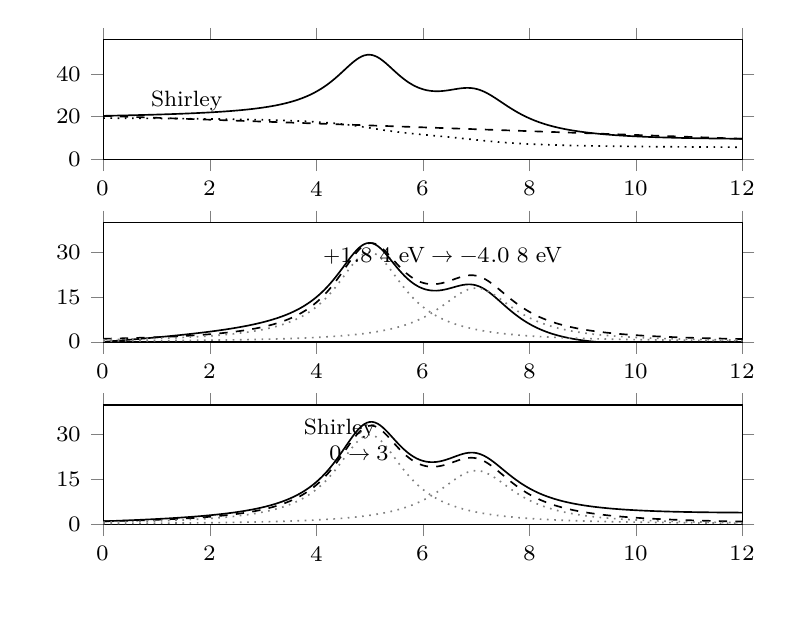
\begin{tikzpicture}
\tikzset{declare function={
  lor(\x,\a,\w)=1/(1+((\x-\a)/\w)*((\x-\a)/\w));
  pA(\x)=30*lor(\x,5,0.8);
  pB(\x)=18*lor(\x,7,0.9);
  cum(\x)=(24*(90-atan((\x-5)/0.8))+16.2*(90-atan((\x-7)/0.9)))*0.0174533;
  bsh(\x)=5+0.1188*cum(\x);
  blin(\x)=20.34-0.8933*\x;
  spec(\x)=pA(\x)+pB(\x)+bsh(\x)+0.25*\x;
}}
\begin{groupplot}[
  group style={group size=1 by 3, vertical sep=8mm},
  width=\onecolwidth,
  height=31mm,
  xmin=0, xmax=12, ymin=0,
  samples=241,
  tick label style={font={\fontsize{8}{9.6}\selectfont}},
  label style={font={\fontsize{8}{9.6}\selectfont}},
  axis line style={line width=0.5pt},
  every axis plot/.append style={line width=0.6pt},
]
\nextgroupplot[ymax=56, ylabel={计数（示意）}, ytick={0,20,40}]
\addplot[black, domain=0:12] {spec(x)};
\addplot[black, dashed, domain=0:12] {blin(x)};
\addplot[black, dotted, domain=0:12] {bsh(x)};
\node[align=left, text width=44mm, anchor=north west,
      font={\fontsize{8}{9.6}\selectfont}] at (rel axis cs:0.03,0.97)
      {实线：模型谱\\ 虚线：线性背景\\ 点线：Shirley 背景};
\nextgroupplot[ymax=40, ylabel={计数（示意）}, ytick={0,15,30}]
\addplot[black, domain=0:12] {spec(x)-blin(x)};
\addplot[black, dashed, domain=0:12] {pA(x)+pB(x)};
\addplot[gray, dotted, domain=0:12] {pA(x)};
\addplot[gray, dotted, domain=0:12] {pB(x)};
\node[align=left, text width=52mm, anchor=north east,
      font={\fontsize{8}{9.6}\selectfont}] at (rel axis cs:0.97,0.97)
      {线性背景扣除后\\ 残差 $+1.8$（4 eV）$\to$ $-4.0$（8 eV）\\ 符号反转：必须改组分比};
\nextgroupplot[ymax=40, xlabel={结合能（相对标度）}, ylabel={计数（示意）}, ytick={0,15,30}]
\addplot[black, domain=0:12] {spec(x)-bsh(x)};
\addplot[black, dashed, domain=0:12] {pA(x)+pB(x)};
\addplot[gray, dotted, domain=0:12] {pA(x)};
\addplot[gray, dotted, domain=0:12] {pB(x)};
\node[align=left, text width=52mm, anchor=north east,
      font={\fontsize{8}{9.6}\selectfont}] at (rel axis cs:0.97,0.97)
      {Shirley 背景扣除后\\ 残差为 $0\to3$ 的平缓斜坡\\ 不造成组分比的系统偏差};
\end{groupplot}
\end{tikzpicture}
\caption{模型计算：同一张谱分别用线性背景（中）与 Shirley 背景（下）扣除后的双峰分解差异。读者应比较两个残差：中图残差在 4 eV 附近为 $+1.8$、在 8 eV 附近为 $-4.0$，\emph{出现符号反转}，说明背景拿走了本属于峰或留下了本属于背景的强度，且高低结合能端方向相反，无法靠微调峰面积吸收，只能改变两个组分的比例才能收敛；下图残差只是 $0\to3$ 的单调斜坡，不会造成组分比的系统偏差。图内实线为谱，粗虚线为固定的双峰模型和，细点线为两个组分。条件与局限：两个 Lorentz 型组分（峰位 5 与 7、半高宽 1.6 与 1.8、峰高 30 与 18）叠加台阶背景（阶高约 15）与缓升二次电子背景，未含真实谱的卫星峰、多重分裂与统计噪声；在本示意参数下改用线性背景使高结合能组分的表观相对含量下降约 25\%—30\%。\modelmark\figsrc{本图为模型计算，源文件无对应图}}
\label{fig:ch09-bgfit}
\end{figure}

\paragraph{读图实例：背景模型如何改变组分比}
\begin{obs}
图 \figref{fig:ch09-bgfit} 中，模型谱由两个 Lorentz 型组分叠加台阶背景与缓升的二次电子背景构成。用线性背景扣除后，与"固定峰位、固定半高宽的双峰模型"相减得到的残差在低结合能端为正（约 $+1.8$）、在高结合能端为负（约 $-4.0$），出现符号反转；用 Shirley 背景扣除后，残差只是一条 $0\to3$ 的平缓单调斜坡，没有符号反转。
\end{obs}
\begin{infer}
残差符号反转意味着背景模型在高、低结合能端分别多扣与少扣了强度，方向相反，无法靠微调某一峰的面积同时吸收，只能\emph{改变两个组分的比例}才能收敛。也就是说：同一张谱、同一组峰位与半高宽，仅更换背景模型，就会得到不同的化学态比例。在本示意参数下，改用线性背景使高结合能组分的表观相对含量下降约 25\%—30\%。
\emph{核对说明}：已对照原页面图像（书内 p.634—p.635 / PDF p.125—p.126）。原书讨论本底扣除时只作定性比较：线性扣除法适合纯金属样品、方法简单可操作性强但缺乏理论依据，非线性扣除法适合所有样品（书内 p.634）；图 9-79 以 Fe 2p 为例给出选点不同造成的峰面积差——线性本底 1 点峰面积 44560、2 点 66589（差 22029），非线性本底 1 点 41167、2 点 49814（差 8647），原书并未把它折算为组分比偏差，也没有本节这样的双峰模型算例。故本处「15\%—20\%」由本图模型参数（两 Lorentz 组分的峰位 5 与 7、半高宽 1.6 与 1.8、峰高 30 与 18，台阶背景阶高约 15）解析估算得出，未做数值积分，属本改编本的模型估算，原书无同类算例可对照。
\end{infer}

\begin{pitfall}
（1）把分峰结果当唯一解：换背景、换端点、换 GL 比例、换峰数都能得到"看起来一样好"的拟合（$\chi^{2}$ 差不到 1\%，组分比却可能差 30\%）。（2）背景端点选在峰的尾部而不是平坦区，系统性过扣。（3）固定了半高宽却不固定自旋轨道分裂与面积比，造出并不存在的物种。（4）用 C 1s 284.8 eV 标定本身含碳的样品（见 §\ref{sec:ch09-problems}）。（5）用未扣背景的原始谱直接比较峰高——峰高受半高宽与背景影响，只有面积才有物理意义。（6）只看拟合优度，不看化学合理性。
\end{pitfall}

\begin{crosscheck}
（1）用同一元素的另一根谱线（Ni 2p 与 Ni 3p、Cu 2p 与 Cu 3p）独立拟合，两组分比应一致；（2）用 Auger 参数交叉验证化学态归属；（3）换两种背景模型、两种端点重复拟合，组分比变化应小于 10\%，否则只能报区间；（4）用不同取出角或不同动能谱线检查是否存在深度不均；（5）与 XANES／EXAFS、Raman、\ce{H2}-TPR 等独立技术对照。
\end{crosscheck}

\subsection{XPS 实验中的常见问题}
\label{sec:ch09-problems}

\emph{核对说明}：本节有原书对应正文，已对照原页面图像（书内 p.640—p.641 / PDF p.131—p.132）并通查其 OCR 全文（\texttt{sources/parts/ch09-b.txt} 第 780 行起，即原书 §9.2.10「XPS 分析中常遇到的一些问题」，书内 p.640 起）。原书列举的问题为：XPS 的检出范围、信号强度与分辨能力、谱仪的能量标尺校准、XPS 的伴峰、绝缘样品表面的荷电校正、各种谱线的重叠、对被测样品的要求、实验中 X 射线对样品表面的副效应等，并按「1. XPS 的检出范围」「2. 信号强度与分辨能力」逐条展开。原书用「检出范围」而不用「检出限」，并在脚注中写明「有种提法为所谓的『检出限』，这种提法不妥。实际上无检出极限，因为辐射源的功率可再提高，检测器的灵敏度也可再提高」；早期仪器相对灵敏度约 1\%（相对原子百分比），现在可达约千分之一。本节把常见问题重组为荷电、污染、X 射线损伤、差分荷电、样品制备假象五类并按「症状—判据—处置」列表，属按学科标准形式与仪器惯例的改编补充，与原书的分类与叙述顺序不同；数量级（约 0.1—1 at\%）与原书一致。

\begin{probout}
把"样品问题"与"样品本征性质"分开，是 XPS 实验设计的第一要务。以下五类问题覆盖了绝大多数误判：荷电、污染、X 射线损伤、差分荷电、样品制备引入的假象。每一类都按"症状 $\to$ 判据 $\to$ 处置"给出可操作流程（表 \tabref{tab:ch09-problems}）。
\end{probout}

\begin{table}[tbp]
\centering
\caption{XPS 实验中的常见问题：症状、判据与处置。判据一栏给的是可以在谱图上直接核对的量，凡判据不成立就不要把现象写成结论。\src{本表为本改编本归纳，非源书表格；本节源文件中无对应 OCR 文本，五类问题的症状、判据与处置按学科标准形式与仪器惯例归纳，待回查原书。}}
\label{tab:ch09-problems}
{\fontsize{8}{9.6}\selectfont
\begin{tabular}{@{}p{15mm}p{36mm}p{40mm}p{48mm}@{}}
\toprule
问题 & 典型症状 & 判据（可直接核对） & 处置 \\
\midrule
荷电（整体） & 全部峰向高结合能整体平移 1—10 eV，峰形不变；平移量随 X 射线通量与时间变化 & 降低通量或开启中和枪后\emph{所有}峰同步回移；各元素峰的位移量一致 & 降低通量、开中和枪、改善与样品台的接触（压薄、压实在台上、金箔搭接）；用内标校准并写明所用参考与 $\pm0.2$ eV 的不确定度 \\
表面污染 & C 1s 与 O 1s 随时间增强；表面金属组分（Ni 2p、Co 2p）相对含量下降；C 1s 在 286—289 eV 出现组分 & 抽真空时间越长污染越重；新解理或刚刻蚀后立即测量则显著减弱；空白样品台与胶带在同条件下出现同样的 C／O & 缩短样品在分析室的停留时间；先低分辨快速扫一遍再定条件；必要时加热除气或轻刻蚀（会改变表面状态，须对照）；报数时说明污染层是否计入总量 \\
X 射线损伤 & 低价态随时间单调增长（\ce{Cu^{2+}}$\to$\ce{Cu+}、\ce{Mo^{6+}}$\to$\ce{Mo^{4+}}、\ce{Ce^{4+}}$\to$\ce{Ce^{3+}}）；聚合物脱氟、C—O 组分增强、O 1s 增强 & 同一位置连续采集 8—10 次，价态比或峰形随累积剂量\emph{单调}变化；移动到未照射的新位置后恢复 & 降低 X 射线功率、用单色器、缩短单次采集多点平均、低温台；先测最敏感的元素；用剂量序列外推到零剂量 \\
差分荷电 & 同一元素的峰展宽或分裂，间距随通量／时间变化；样品峰与污染碳峰的漂移量不一致 & 分裂间距与已知化学位移不符；降低通量或改善电接触后分裂消失；样品峰与内标峰给出的 $\Delta$ 不同 & 重新制样（压薄压实、导电胶或金箔搭接）、降低通量、适当中和；用第二根谱线（如 Ni 3p）与双内标验证后重测 \\
制备假象 & 出现与制备过程有关的元素（Si、Na、F、S、增塑剂）；刻蚀后出现 Ar、低价态或组分突变；颗粒表面出现异常氧化物 & 空白对照（胶带、溶剂、模具、\ce{Ar+} 刻蚀）在同条件下测出相同指纹；未处理的同批样品无此信号 & 改用无胶带固定（压片、金属夹）、换溶剂并充分干燥、避免过度研磨；刻蚀条件先用已知厚度标样标定速率并做空白；完整记录样品历史 \\
\bottomrule
\end{tabular}}
\end{table}

\begin{principle}
\emph{荷电}：光电离不断把电子送出样品，绝缘样品表面累积正电荷，稳态电位由 X 射线通量、样品电导、与样品台的接触、二次电子与中和电子的供给共同决定，因此它随时间、位置与通量漂移（表现为整体平移，不改变峰形）。\emph{污染}：真空中残余的 \ce{H2O}、CO 与碳氢化合物吸附在表面，并被 X 射线与二次电子诱导分解，形成 1—3 nm 的碳质层，厚度随抽真空时间增长。\emph{X 射线损伤}：二次电子与 Auger 过程造成键断裂与脱附——聚合物交联或脱氟，金属氧化物被还原（\ce{Cu^{2+}}$\to$\ce{Cu+}、\ce{Mo^{6+}}$\to$\ce{Mo^{4+}}、\ce{Ce^{4+}}$\to$\ce{Ce^{3+}}），表现为"低价态"随时间增长。\emph{差分荷电}：同一视场内不同区域、不同颗粒、污染层与基体之间的电导不同，各自建立不同的稳态电位，于是同一元素的谱线出现\emph{随通量与时间变化的}展宽或分裂——它不是化学位移。\emph{制备假象}：研磨引入氧化物与相变，胶带与脱模剂引入 Si、Na、增塑剂，溶剂残留引入 C—O、F、S，\ce{Ar+} 刻蚀引入择优溅射、离子束还原、Ar 植入与表面粗糙化。
\end{principle}

\begin{measure}
诊断性实验设计（按代价从低到高）：
\begin{enumerate}
\item \emph{时间序列}：固定位置连续采集 8—10 次同一窄扫，作峰位、半高宽、组分比随累积剂量的变化曲线。峰位单调漂移或低价态单调增长 $\Rightarrow$ 损伤或荷电；峰形不变而只整体平移 $\Rightarrow$ 荷电。
\item \emph{通量序列}：把 X 射线功率降低 3—5 倍重测。峰位随通量变化 $\Rightarrow$ 荷电；峰位不变而低价态比例明显下降 $\Rightarrow$ 损伤。
\item \emph{中和枪开／关对照}：只影响荷电，不影响污染与损伤。
\item \emph{位置对照}：移到未照射过的新位置立即采集。若"低价态"消失 $\Rightarrow$ 是束流效应而不是样品本征。
\item \emph{取出角序列}（15°／45°／90°）：判断污染层与深度分布，也用于验证"表面富集"是否真在表面。
\item \emph{空白对照}：样品台、胶带、溶剂、压片模具在同条件下各测一次，建立污染指纹库。
\item \emph{记录样品历史}：暴露空气时长、研磨与压片方式、溶剂与粘接方式，以及本次测量的时刻。
\end{enumerate}
\end{measure}

\begin{dataflow}
症状 $\to$ 判据（可量化的阈值，见表 \tabref{tab:ch09-problems}）$\to$ 处置 $\to$ 复测确认（问题是否消失或减轻）$\to$ 写结论时必须同时写明限制条件（是否含污染层、是否可能有损伤、是否做过荷电校准及所用参考）。
\end{dataflow}

\paragraph{读谱实例：看着像两个价态，其实是差分荷电}
\begin{obs}
Ni 2p$_{3/2}$ 区主峰半高宽由正常的约 1.4 eV 展宽到 3.2 eV，峰形不对称；强行拟合成两个峰得到 855.2 eV 与 857.4 eV，间距 2.2 eV，面积比约 1.5:1。连续采集 6 次后主峰位置由 855.2 eV 漂到 856.1 eV，而同时记录的污染碳 C 1s 只漂移 0.1 eV；把 X 射线功率降低 5 倍后，峰位回移约 0.6 eV，峰形变窄。
\end{obs}
\begin{infer}
三条判据都指向\emph{差分荷电}，而不是"两个价态"：（a）Ni 2p 的化学位移通常在 1—1.5 eV 量级，且不同价态伴随不同的卫星峰结构，2.2 eV 的分裂与常见价态对不上；（b）化学态比例不应随 X 射线功率变化；（c）样品峰与污染碳峰的漂移量不一致，说明两者处在不同电位上。\emph{处置}：重新制样（压薄、压实在样品台上，边缘用导电胶或金箔搭接）、降低 X 射线通量、适当中和后重测；并用同一元素的第二根谱线（Ni 3p）与双内标（C 1s 与 Au 4f$_{7/2}$）比对平移量来验证。
\end{infer}

\begin{pitfall}
四条最常见的误判，以及各自的判据与处置：
\begin{enumerate}
\item \textbf{把分峰结果当唯一解}。判据：换背景、换端点或换 GL 比例后组分比变化超过 10\%。处置：做敏感性分析，报组分比的区间而不是单值，并在正文写明约束条件。
\item \textbf{用 C 1s 284.8 eV 标定，而样品本身就有碳物种}。判据：样品合成或组成中含碳（碳化物、石墨、\ce{C60}、聚合物、有机配体、碳酸盐），或 C 1s 峰形不对称、半高宽大于 2 eV、在 286—290 eV 还有组分。处置：改用样品自身已知物种（晶格氧、金属态、费米边）或 Au 4f$_{7/2}$ 内标，或者明确按"未做荷电校准、只报相对位移"处理，并把所用参考写进正文。
\item \textbf{把差分荷电当成多价态}。判据：分裂间距与已知化学位移不符、峰位随通量／时间／位置变化、样品峰与内标峰漂移不一致、改善电接触或降低通量后分裂消失（见上面的读谱实例）。
\item \textbf{定量不报误差与检出限}。判据：只给"某元素 $=$ x at\%"而不给不确定度、检出限与是否计入污染碳。处置：报原子分数 $\pm$ 相对不确定度（同批比较 $\pm5\%\sim\pm10\%$，绝对 $\pm20\%\sim\pm30\%$），注明检出限（约 0.1—1 at\%）与归一化范围（不含 H）。
\end{enumerate}
此外还有两条同样常见：把 shake-up 伴峰或 X 射线卫星线当独立化学态定量；把 \ce{Ar+} 刻蚀后的结果当作原始表面状态。
\end{pitfall}

\begin{crosscheck}
XRD 回查体相物相；XANES／EXAFS 回查价态与配位（且可在原位气氛下测量，避免样品离开气氛后重构）；Raman 与 IR 回查碳物种与官能团；\ce{H2}-TPR 回查可还原性。最有力的一个交叉检验是\emph{换激发源}：芯能级结合能不随光子能量变化，而 Auger 峰动能不变（于是它的表观结合能随 $h\nu$ 平移）。若一个"化学态"的位置随激发源改变，它多半是 Auger 峰或卫星线的误判。
\end{crosscheck}

\srcnote{本分片按任务书覆盖 §9.2.7—§9.2.10。价带谱与 shake-up 伴峰部分取自源文件 \texttt{ch09-d.txt} 的 §9.6.2（书内 p.705—708 / PDF p.196—199，已对照页面图像）及表 9-37（书内 p.712 / PDF p.203，已对照页面图像）；§9.2.7—§9.2.10 的原书正文本身见书内 p.623—641，其 OCR 文本在另一分片的源文件 \texttt{sources/parts/ch09-b.txt}（§9.2.7 第 227 行／§9.2.8 第 415 行／§9.2.9 第 589 行／§9.2.10 第 780 行）。定量、后处理与常见问题三节的公式、常数与分类为按学科标准形式与仪器惯例的改写：与原书形式一致之处、原书未给出或未印之处，逐条记于各节前的核对说明。}
}{}
\IfFileExists{chapters/parts/ch09-e.tex}{\input{chapters/parts/ch09-e}}{}
}{}
\IfFileExists{chapters/ch10.tex}{% chapters/ch10.tex —— 第 10 章 多相催化反应动力学
% 装配层：只负责按顺序引入各分片。分片缺失时跳过，便于增量成书。
% 分片文件：chapters/parts/ch10-{a..e}.tex

\IfFileExists{chapters/parts/ch10-a.tex}{% ================================================================
%  chapters/parts/ch10-a.tex
%  第 10 章  多相催化反应动力学（分片 a）
%  源：S2（下册）第 10 章，书内 p.735—768 / PDF p.225—257
%  覆盖：10.1 一般动力学概念；10.2 吸附和多相催化反应速率方程
%  未覆盖：10.3 及以后（模型建立与检验、回归实例、非均匀表面）→ 分片 b/c
% ================================================================

\chapterstart{多相催化反应动力学}%
{本章导读：多相催化动力学最终要交付一个能用的速率方程，而方程的形式只由两件事决定——
哪一步最慢（速率控制步骤，RDS），以及吸附平衡如何把表面覆盖度换算成流体相浓度。分片 a
先建立可测的宏观量（化学计量数、反应度、速率、转换频率、理想反应器积分式），再引入吸附
等温方程与 RDS，推出双曲线式与幂式两类速率方程，并说明表观活化能为何不等于真实活化能。
模型检验、传递过程与测定方法见后续分片。}
\label{ch:10}

\subsection{一般动力学概念}

\begin{probout}
化学动力学研究一个化学物种转化为另一物种的\textbf{速率}与\textbf{机理}。在多相催化中，
「速率」指单位时间、单位反应空间（含催化剂量）内某反应物的消耗量或某产物的生成量；
「机理」指达成该反应的全部基元步骤序列——不仅包括表面上的化学变化，还包括吸附、脱附
和相间／粒内传递。因此多相催化速率方程比匀相多两层结构：\textbf{传递是否限制}，以及
\textbf{表面覆盖度如何随流体相组成变化}。本分片要回答三个问题：速率的可测定义是什么、
RDS 假设如何把覆盖度翻译成浓度依赖、以及为什么同一套数据能被几个机理同时拟合。
\end{probout}

对一个化学物种，从流体到产物要经历「相间扩散 → 粒内扩散 → 吸附 → 表面反应 → 脱附 →
粒内扩散 → 相间扩散」。把其中的\textbf{化学变化基元步骤序列}称为历程，把\textbf{含吸附、
脱附与传递过程的完整序列}称为机理。传递过程是否构成阻力，由后续分片讨论；本分片只在
「表面过程为唯一阻力」的假设下展开。\src{S2 第 10 章引言，书内 p.737 / PDF p.226}

从动力学角度，有工业意义的多相催化反应可分为消除反应（脱氢、脱水、裂化等）、双组元加成
反应（加氢、氧化、歧化、烃化等）和多组元加成反应（氨氧化、氧氯化、羰基合成等）三类；
它们本身是简单反应，但在同一催化剂上常以不同程度同时或相继进行，构成\textbf{连串}、
\textbf{平行}或\textbf{连串-平行}的复杂反应网络。组分越多，动力学解析越难；而任意简化
又会使模型面目全非——这是本章始终要权衡的一对矛盾。\src{S2 §10 引言，书内 p.737—739 /
PDF p.226—228}

\subsubsection{化学计量方程、基元反应与反应途径}

任何化学反应（总包反应或基元步骤）都可写成
\begin{equation}
\nu_1\mathrm{B}_1+\nu_2\mathrm{B}_2+\cdots \rightleftharpoons
\nu_3\mathrm{B}_3+\nu_4\mathrm{B}_4+\cdots
\quad\text{或}\quad \sum_i \nu_i\mathrm{B}_i=0
\label{eq:stoi}
\end{equation}
式中 $\nu_i$ 为组分 $\mathrm{B}_i$ 的化学计量数：$\nu_i>0$ 为产物，$\nu_i<0$ 为反应物。
\src{S2 §10.1.1，书内 p.739 / PDF p.228，式(10-1)}

\textbf{化学计量方程本身不能说明分子水平上发生了什么，除非它写的是基元步骤。}对基元
反应，计量数固定且必须按分子水平实际发生的过程书写。例如氧分子在活性位上的解离吸附：

\begin{equation}
\mathrm{O_2}+2* \rightleftharpoons 2\,\mathrm{O}{*}
\qquad\text{不能写作}\qquad
\tfrac{1}{2}\mathrm{O_2}+2* \rightleftharpoons \mathrm{O}{*}
\label{eq:elem}
\end{equation}
式中 $*$ 为表面活性位。后一种写法在计量上等价，但从机理上无意义——它把一个双位解离
过程写成了单位过程。\src{S2 §10.1.2，书内 p.739 / PDF p.228}

催化剂通过一组基元反应把反应物转化为产物、自身又回到初始状态，这一闭合循环称为
\textbf{催化循环}；循环中各基元步骤加和而成的总反应称为\textbf{总包反应}；基元步骤的
顺序称为\textbf{反应途径}（反应序列）。三者的可测性不同：\textbf{总包反应的反应物与产物
都在流体中，是可测的；基元步骤与中间物种通常不可直接测}，只能靠动力学与谱学证据推断。

\subsubsection{反应度、反应速率与速率方程}

对式~\eqref{eq:stoi}，组分 $\mathrm{B}_i$ 的反应度定义为

\begin{equation}
\dd\xi_i=\nu_i^{-1}\dd n_i
\qquad\Longrightarrow\qquad
\frac{\dd\xi_i}{\dd t}=\nu_i^{-1}\frac{\dd n_i}{\dd t}
\label{eq:xi}
\end{equation}
式中 $n_i$ 为 $\mathrm{B}_i$ 的物质的量；$\dd\xi_i$ 可正可负，视 $\nu_i$ 的正负而定。
反应速率 $r_i$ 定义为反应度对时间的导数除以反应空间：

\begin{equation}
r_i=\frac{1}{Q}\frac{\dd\xi_i}{\dd t}
=f(k,T,c_i)=f(k,T,p_i)
\label{eq:rate-def}
\end{equation}
式中 $Q$ 为催化剂的质量、体积或比表面积；相应地 $r_i$ 是单位质量、单位体积或单位比表面积
上的\textbf{比速率}。$Q$ 的选择决定了 $r$ 的数值与量纲，也决定了速率常数 $k$ 的量纲——
\textbf{不同 $Q$ 基准下的 $k$ 不可直接比较}。式~\eqref{eq:rate-def} 表达了速率与温度、
浓度的函数关系，称为\textbf{速率方程}（微分表达式）；若表达的是接触时间、温度与转化率、
生成率之间的关系，则称为\textbf{积分表达式}。\src{S2 §10.1.3，书内 p.739—740 /
PDF p.228—229，式(10-2)—(10-5)}

对封闭系统的均相反应，$Q$ 即反应体积 $V$，速率是浓度的幂函数：
\begin{equation}
r_i=\frac{1}{\nu_i}\frac{\dd c_i}{\dd t}=k\prod_i c_i^{m_i}
\label{eq:power}
\end{equation}
式中 $k$ 只是温度的函数，与浓度无关；$m_i$ 为对组分 $\mathrm{B}_i$ 的\textbf{反应级数}，
可为整数或分数、正数或负数，也可为零。式~\eqref{eq:power} 形式的速率方程称为
\textbf{幂式速率方程}。\src{S2 §10.1.3，书内 p.740 / PDF p.229，式(10-6)、式(10-7)}

\begin{keycond}
式~\eqref{eq:rate-def} 的用法有两条硬约束。（1）\textbf{必须声明 $Q$ 基准}：单位质量、
单位体积还是单位比表面积；否则「速率」数值无意义。（2）\textbf{必须声明反应度或转化率的
测量点}：多相催化中速率随转化率变化，同一个催化剂在不同转化率下给出不同的 $r$。只有在
转化率足够小（近似初始速率）时，$r$ 才近似为组成的单一函数。
\end{keycond}

\subsubsection{Arrhenius 定律、活化能与表观活化能}

\begin{principle}
\textbf{Arrhenius 定律。}单一基元反应的速率常数服从
\begin{equation}
k=A_0\exp\!\left(-\frac{E}{RT}\right)
\label{eq:arrh}
\end{equation}
式中 $A_0$ 为频率因子（指前因子），$E$ 为活化能。\textbf{成立条件}：$E$ 在所考察温度区间
内近似为常数，且反应按同一基元步骤进行。\textbf{量纲检查}：$\exp(-E/RT)$ 无量纲，故 $A_0$
与 $k$ 同量纲；$k$ 的量纲由速率方程形式与 $Q$ 基准共同决定（例如一级反应取 $Q=V$ 时
$k$ 为 $\mathrm{s^{-1}}$；取 $Q=$ 催化剂质量时为 $\mathrm{m^3{\cdot}g^{-1}{\cdot}s^{-1}}$）。
\textbf{因此比较活化能时必须先统一速率方程形式与 $Q$ 基准}，否则比的是两个不同的量。
\end{principle}

对由一系列基元步骤构成的多相催化反应，\textbf{整个反应的速率常数仍符合 Arrhenius 定律}，
但此时 $A_0$ 称为指前因子、$E$ 称为\textbf{表观活化能}。动力学参数一般指速率常数、反应
级数、指前因子和活化能（表观活化能）。\src{S2 §10.1.3，书内 p.740 / PDF p.229，式(10-8)}

最稳妥的表观活化能定义是 Arrhenius 图的\textbf{局部斜率}：
\begin{equation}
E_{\mathrm{app}}\equiv -R\,\frac{\partial \ln r}{\partial (1/T)}\Bigg|_{c_i\ \text{恒定}}
\label{eq:eapp-def}
\end{equation}
把 $E_{\mathrm{app}}$ 写成式~\eqref{eq:arrh} 那样的单一常数，本身就是一个假设。它何时成立、
何时失效，见 §\ref{sssec:eapp}。

\subsubsection{转换数与转换频率（TOF）}

\begin{principle}
\textbf{转换数（turnover number，TON）}：通过催化循环发生的总包反应次数，
\begin{equation}
\mathrm{TON}=\xi N_{\mathrm A}
\label{eq:ton}
\end{equation}
式中 $\xi$ 为在催化剂上转化的物质的量，$N_{\mathrm A}$ 为阿伏伽德罗常量。于是反应速率可写作
$v=\dd(\mathrm{TON})/\dd t$。\textbf{转换频率（turnover frequency，TOF）}：在给定温度、
压力、反应物比率及一定反应度下，单位时间内单位活性位上发生的转换数，
\begin{equation}
\mathrm{TOF}=\frac{1}{S}\frac{\dd(\mathrm{TON})}{\dd t},
\qquad S=[L]\,A
\label{eq:tof}
\end{equation}
式中 $S$ 为实验中起作用的活性位数，$[L]$ 为活性位密度（单位面积上的活性位数），$A$ 为
催化剂的总活性表面积。\textbf{量纲检查}：$\mathrm{TON}$ 若以分子数计，$S$ 也须以活性位
个数计，$\mathrm{TOF}$ 的量纲为 $\mathrm{s^{-1}}$；若两者都改用 mol 基准，比值不变，仍为
$\mathrm{s^{-1}}$。但\textbf{不可一个用 mol、一个用个数}，那样会差 $N_{\mathrm A}$ 倍。
\end{principle}

TOF 的优点是其量纲为时间的倒数，便于不同研究者的结果互相比较。\textbf{但可比性有前提，
缺一条就不能比。}

\begin{measure}
\textbf{TOF 的测量与报告条件。}（1）\textbf{活性位数 $S$ 必须由化学吸附滴定测定}
（\ce{H2}、\ce{O2}、\ce{CO} 脉冲吸附或选择性化学吸附），且滴定本身要独立证明化学计量比
（H/M、O/M、CO/M）；用 BET 面积或总表面积推算 $S$，等于把「几何面积」当作「活性位数」，
TOF 随之失去意义。（2）\textbf{必须声明全部反应条件}——温度、压力、反应物比率、反应度或
转化率；TOF 是速率而不是速率常数。（3）\textbf{必须取微分（低转化率）条件}：若存在内、外
扩散限制或转化率过高，测到的是被传递过程和产物抑制修饰过的表观速率，TOF 被系统性压低。
（4）\textbf{活性位的定义在样品间要一致}：不同晶面、不同尺寸的活性位本征 TOF 不同，实测值
是\textbf{平均值}。活性位的计数方法与化学吸附滴定的实验细节见\chapref{ch:05}；本分片只
使用其结果，不重复推导。\src{S2 §10.1.4，书内 p.740—741 / PDF p.229—230，式(10-9)—(10-12)}
\end{measure}

\begin{pitfall}
\textbf{把 TOF 当作速率常数用。}TOF 是速率，随压力、组成和覆盖度变化。文献中「催化剂 A 的
TOF 是 B 的 5 倍」这类比较，只有在同温度、同分压、同转化率、同活性位计数方法下才成立。
另一常见误用是把 TOF 与转换率（conversion）混为一谈：前者是单位活性位的速率，后者是
反应物的转化分数，两者量纲与含义都不同。
\end{pitfall}

\subsubsection{碰撞理论与过渡态理论}

两个理论都想为式~\eqref{eq:arrh} 中的 $A_0$ 与 $E$ 找理论根据，但适用范围都很有限。

\textbf{碰撞理论}（20 世纪 20 年代末，Lewis、Polanyi 等）把分子视为刚性圆球。$\mathrm{B}_1$
与 $\mathrm{B}_2$ 的碰撞次数为
\begin{equation}
Z=c_1c_2\sigma_{12}^{2}
\left(\frac{8\pi RT\,(M_1+M_2)}{M_1M_2}\right)^{1/2}
\label{eq:coll}
\end{equation}
式中 $c_i$ 为单位体积中 $\mathrm{B}_i$ 的分子数，$M_i$ 为相对分子质量，$\sigma_{12}$ 为碰撞中
两分子的有效直径。速率等于碰撞数乘以能量在 $E$ 以上的分子比例
$f_{\mathrm c}=\exp(-E/RT)$，与 $r=kc_1c_2$ 对比即得 $A_0$。\textbf{量纲检查}：$c$ 为
$\mathrm{m^{-3}}$、$\sigma$ 为 $\mathrm{m}$、$(M_1+M_2)/(M_1M_2)$ 为
$\mathrm{mol{\cdot}kg^{-1}}$，与 $RT$ 相乘开方后为 $\mathrm{m{\cdot}s^{-1}}$，故 $Z$ 的量纲
为 $\mathrm{m^{-3}{\cdot}s^{-1}}$，自洽。该理论对少数双分子气体反应成功，但对很多反应预测
的 $A_0$ 比实测值高几个数量级。\src{S2 §10.1.5，书内 p.741—742 / PDF p.230—231，
式(10-13)—(10-17)}\tocheck{未对照原页面图像：式~\eqref{eq:coll} 的 OCR 作 $\sigma_{12}$
而非 $\sigma_{12}^{2}$；按量纲与标准形式应为 $\sigma_{12}^{2}$，此处按标准形式重建。}

\textbf{过渡态理论}（20 世纪 30 年代末）认为反应经碰撞生成过渡态
$(\mathrm{B}_1\mathrm{B}_2)^{*}$，它与反应物处于热力学平衡，其分解为控速步骤，分解频率
$f_{\mathrm t}=k_{\mathrm B}T/h$，故 $r=(k_{\mathrm B}T/h)[\mathrm{B}_1\mathrm{B}_2]^{*}$。
把过渡态浓度按平衡式代入并与式~\eqref{eq:arrh} 对比，可得频率因子的理论表达式：
\begin{equation}
A_0=\frac{k_{\mathrm B}T}{h}\exp\!\left(1-\Delta n+\frac{\Delta S^{*}}{R}\right)
\label{eq:tst}
\end{equation}
式中 $k_{\mathrm B}$ 为玻尔兹曼常量，$h$ 为普朗克常量，$\Delta S^{*}$ 为过渡络合物与反应物
之间的熵差，$\Delta n$ 反映活化过程中分子数的变化。
\tocheck{未对照原页面图像：式~\eqref{eq:tst} 中 $(1-\Delta n)$ 一项的符号与 $\Delta n$ 的
基准（原书正文写作「与反应物和产物的分子数之差」，与式(10-20) 中
$\Delta H^{*}=E-RT+\Delta nRT$ 的活化过程基准不一致）无法从 OCR 确认，此处按
「$\Delta n=$ 过渡态分子数 $-$ 反应物分子数」重建。}\textbf{理论上可由过渡态构型计算
$\Delta H^{*}$ 与 $\Delta S^{*}$ 从而得到 $A_0$ 与 $E$，但仅对简单分子可行}；对结构复杂的
反应尚受很大限制，对多相催化反应更只能给出定性理解。\src{S2 §10.1.5，书内 p.742—743 /
PDF p.231—232，式(10-18)—(10-21)}

\subsubsection{理想反应器中的反应速率}

反应器中各点的反应速率并不相同，可观测的总包速率是各点速率（point rate）的集合，因此
\textbf{动力学方程与反应器类型绑定}。化学工程学按停留时间分布建立两类理想反应器模型：
连续搅拌釜式反应器（CSTR）与活塞流反应器（PFR）。\src{S2 §10.1.6，书内 p.743 /
PDF p.232}

\textbf{CSTR} 的基本假设是：反应器内流体粒子理想混合，浓度与温度均匀；出口流体参数与
器内物料完全相同。故定态下反应速率处处相等，
\begin{equation}
r=\frac{n_0-n_{\mathrm f}}{V/F}=\frac{n_0-n_{\mathrm f}}{\tau}
\label{eq:cstr}
\end{equation}
式中 $n_0$、$n_{\mathrm f}$ 为单位质量进、出反应器物流中关键组分的摩尔数，$F$ 为单位时间
进料质量，$V$ 为反应器容量，$\tau$ 为空时。这是\textbf{代数方程，不存在积分问题}——这是
CSTR 在动力学测定中最大的优点。

\textbf{PFR} 的基本假设是：流体微元以相同线速度沿轴向运动、停留时间相同、流动方向上无
混合，同一横截面上参数相等。对体积元 $\dd V$ 作物料衡算得 $r\,\dd V=F\,\dd x$，即
\begin{equation}
r=\frac{\dd x}{\dd(V/F)},
\qquad
\frac{V}{F}=\int_0^{x}\frac{\dd x}{r}
\label{eq:pfr}
\end{equation}
式中 $x$ 为单位进料质量的 $\mathrm{B}$ 转化摩尔数。催化反应器更多用催化剂重量微元
$\dd W$，相应有 $r\,\dd W=F\,\dd x$ 与 $W/F=\int_0^x\dd x/r$。
\src{S2 §10.1.6，书内 p.743—744 / PDF p.232—233，式(10-22)—(10-27)}

\begin{keycond}
理想反应器模型的三条边界。（1）\textbf{等温}：非等温床层中 $T$ 沿轴向变化，$k$ 随之变化，
式~\eqref{eq:pfr} 必须与能量衡算联立。（2）\textbf{无返混、无沟流}：固定床在管径／粒径比
过小或存在壁效应时偏离活塞流假设。（3）\textbf{无内外扩散限制}：否则测得的不是表面反应
速率，式~\eqref{eq:pfr} 积分得到的是表观参数。传递过程的多相催化动力学见后续分片。
\end{keycond}

\subsubsection{活塞流管式反应器中简单反应的积分式速率方程}

工业上大多数多相催化过程在活塞流管式反应器中进行，故式~\eqref{eq:pfr} 的积分式是本章最
常用的工具。对一级不可逆单组元反应 $r_1=kp_1$，按理想气体处理有 $p_1=(n_1/n_{\mathrm t})p$；
若反应中摩尔数显著改变，则 $n_{\mathrm t}=n_{\mathrm t0}(1+\omega x)$、$n_1=n_{10}-x$，其中
$\delta$ 为每转化一摩尔所增加的摩尔数、$\omega=\delta/n_{\mathrm t0}$。代入积分得

\begin{equation}
\frac{p}{n_{\mathrm t0}}\frac{V}{F}\,k
=(1+\lambda)\ln\frac{1}{1-X}-\lambda X,
\qquad \lambda=\omega n_{10},\quad X=\frac{x}{n_{\mathrm t0}}
\label{eq:pfr-int}
\end{equation}
若摩尔数无显著改变（定容，$\omega=0$），式~\eqref{eq:pfr-int} 退化为
\begin{equation}
k\,\frac{pV}{n_{\mathrm t0}F}=\ln\frac{1}{1-X}
\qquad\text{或写作}\qquad
k\tau=\ln\frac{1}{1-X}
\label{eq:pfr-int1}
\end{equation}
式中 $\tau$ 为接触时间（可用空时 $V/F$ 换算）。在催化反应中 $V$ 可用催化剂质量 $W$、
表面积 $A$ 或床层长度 $z$ 代替，\textbf{$k$ 的量纲随之改变}。
\src{S2 §10.1.7，书内 p.744—745 / PDF p.233—234，式(10-28)—(10-36)}

\begin{principle}
\textbf{量纲与参数的归属。}式~\eqref{eq:pfr-int} 中的 $k$（以分压为浓度基准、以催化床体积
为反应空间基准时）量纲为 $\mathrm{mol{\cdot}atm^{-1}{\cdot}(床体积)^{-1}{\cdot}时间^{-1}}$；
写成式~\eqref{eq:pfr-int1} 右端的 $k\tau$ 形式时，$k$ 的量纲为 $\mathrm{时间^{-1}}$。
\tocheck{未对照原页面图像：原书把后者标注为「式(10-35) 中的 $k$」，但式(10-35) 是变容式的
定容特例（$k$ 的量纲应与式(10-34) 相同），按上下文应指 $k\tau=\ln[1/(1-X)]$ 的式(10-36)，
此处按后者理解。}\textbf{结论不变}：报告 $k$ 必须同时报告速率方程形式与 $Q$ 基准，否则
不同文献的 $k$ 无法比较。
\end{principle}

\begin{example}[由积分式求接触时间]
教学设定：某一级不可逆反应在定容条件下进行，以接触时间为基准的速率常数
$k=\qty{1.5}{h^{-1}}$。按式~\eqref{eq:pfr-int1}，
$X=0.95$ 时 $\tau=\ln 20/1.5=\qty{2.00}{h}$；$X=0.99$ 时
$\tau=\ln 100/1.5=\qty{3.07}{h}$。\textbf{要点}：一级反应要把转化率从 $95\%$ 提到 $99\%$，
接触时间需再增加约 $50\%$，而转化率的绝对增量只有 $4$ 个百分点。若反应摩尔数显著增加
（$\lambda>0$），同样的转化率需要更长的接触时间，按式~\eqref{eq:pfr-int} 计算。
\pedset{数值为教学设定，非原书实验数据。}
\end{example}

\begin{dataflow}
\textbf{从活塞流积分数据到速率常数。}（1）确认反应器等温、无返混、无内外扩散限制（否则下面
各步得到的是表观参数）。（2）判断反应摩尔数是否显著改变，决定用变容式~\eqref{eq:pfr-int}
还是定容式~\eqref{eq:pfr-int1}。（3）以 $\ln[1/(1-X)]$ 对 $W/F$（或 $V/F$）作图：过原点的
直线支持一级不可逆；明显弯曲或不过原点，则改试幂式的积分形式
（式(10-39)、式(10-41)）或 L-H 型的积分形式~\eqref{eq:lh-int}。（4）在若干温度下重复第
(3) 步，由 $\ln k$ 对 $1/T$ 作 Arrhenius 图求 $E_{\mathrm{app}}$，并\textbf{检查该图是否
弯曲}——弯曲往往意味着覆盖度变化或 RDS 转移（§\ref{sssec:eapp}）。（5）报告时给出速率
方程形式、$Q$ 基准、温度与转化率区间。
\end{dataflow}

对不可逆非一级反应，$r=k(n_1p/n_{\mathrm t})^{m}$，积分得形如
$(V/F)(\cdots)=\int_0^X[(1+\lambda X)/(1-X)]^{m}\dd X$ 的式子；双组元不可逆反应在某一组元
过量（或惰性稀释）且总摩尔数近似不变时，可化为含 $(1-X)^{m_1}(m_0-X)^{m_2}$ 的积分
（$m_0=v_{20}/v_2$）。\textbf{这类积分一般无解析解，需数值积分并配合非线性回归求
$k'$、$m_1$、$m_2$。}\src{S2 §10.1.7，书内 p.746 / PDF p.235，式(10-38)—(10-41)}

\subsubsection{复杂反应的速率方程及其解析}

\textbf{（1）可逆反应。}以 $\mathrm{B_1\rightleftharpoons B_2}$ 的一级可逆反应为例，微分
表达式为 $r=k_1p_1-k_{-1}p_2=k_1(p_1-p_2/K_{\mathrm{eq}})$，代入活塞流积分式可得含
$K_{\mathrm{eq}}$ 的对数式积分表达式。\textbf{关键点}：推动力项写成
$(p_1-p_2/K_{\mathrm{eq}})$ 的形式，使 $r=0$ 自动回到化学平衡——这是速率方程必须满足的
\textbf{热力学一致性}条件，也是对任何机理模型的硬约束。
\src{S2 §10.1.8，书内 p.746 / PDF p.235，式(10-42)、式(10-43)}

\textbf{（2）连串反应与平行反应。}对最简单的连串反应
$\mathrm{B_1\xrightarrow{k_1}B_2\xrightarrow{k_2}B_3}$，中间产物 $\mathrm{B_2}$ 的浓度先
上升较快、达最高点后下降，最终产物 $\mathrm{B_3}$ 起始上升很慢；平行反应的两个产物浓度
起始上升都快，随后趋于各自的渐进线。

\begin{obs}
由浓度-时间曲线可读出：$\mathrm{B}_2$ 的曲线有无极大值、各产物在 $t\to0$ 处的斜率是否
为零。\end{obs}
\begin{infer}
$t\to0$ 斜率近于零的生成物应为\textbf{次级产物}，斜率明显不为零的为\textbf{初级产物}；
据此可确定各产物在反应网络中的位置，再对一级网络估算速率常数。\end{infer}

连串反应可积为 $c_1/c_{10}=\mathrm{e}^{-k_1t}$、
$c_2/c_{20}=[k_1/(k_2-k_1)](\mathrm{e}^{-k_1t}-\mathrm{e}^{-k_2t})$；由 $c_2$ 的极大值
$c_{2\mathrm m}$ 与对应时间 $t_{\mathrm m}=\ln(k_2/k_1)/(k_2-k_1)$ 可图解求 $k_2/k_1$。
该方法方便，但\textbf{过分依赖单个实验点}。
\src{S2 §10.1.8，书内 p.747—748 / PDF p.236—237，式(10-44)—(10-48)}

\begin{pitfall}
\textbf{「出现浓度极大值」不等于「连串历程」。}含可逆步骤的连串历程，中间产物可能不出现
极大值而渐近于一稳定值；反之，某些可逆的平行历程中最终产物却可出现极大值。较可靠的判据
是各产物生成率对接触时间作图后取 $t\to0$ 的斜率，而不是曲线有无极值。
\src{S2 §10.1.8，书内 p.749 / PDF p.238}
\end{pitfall}

\textbf{（3）连串-平行反应}是最常见的工业情形。对
$\mathrm{B_1}\to\mathrm{B_2}$、$\mathrm{B_1}\to\mathrm{B_3}$、
$\mathrm{B_2}\to\mathrm{B_3}$ 组成的最简网络，三个微分方程可积为
$c_1=c_{10}\mathrm{e}^{-(k_1+k_3)t}$ 等解析式，再由 $c_{2\mathrm m}/c_{1\mathrm m}$ 求
$k_1/k_2$、由对数化后的直线求 $k_1+k_3$。\textbf{注意该方法要求 $c_{2\mathrm m}$ 与
$c_{1\mathrm m}$ 测得相当精确。}\src{S2 §10.1.8，书内 p.748—749 / PDF p.237—238，
式(10-49)—(10-52)}

\textbf{（4）近似处理方法。}由复杂历程推导动力学方程时，稳态近似与平衡态近似是两种基本
手段。\textbf{稳态近似}假设中间产物非常活泼、浓度近似与时间无关，如对上述连串反应令
$\dd c_2/\dd t=k_1c_1-k_{-1}c_2-k_2c_2=0$，得 $c_2=k_1c_1/(k_{-1}+k_2)$，进而
$\dd c_3/\dd t=k_1k_2c_1/(k_{-1}+k_2)$。\textbf{平衡态近似}则假设历程中存在速率控制步骤：
当 $k_{-1}\gg k_2$ 时 $c_2\approx(k_1/k_{-1})c_1=Kc_1$，总包速率
$r=k_2Kc_1$。\src{S2 §10.1.8，书内 p.750—751 / PDF p.239—240，式(10-53)—(10-57)}

\begin{principle}
\textbf{平衡态近似（RDS 近似）的操作规则}：若历程中有一个基元步骤为速率控制步骤，则
\textbf{只需写出该步的速率表达式，其中出现的中间产物浓度由与之相关的其他基元步骤的平衡
关系给出}。这条规则是本分片后半部分（§\ref{sssec:rds} 起）全部推导的骨架。
\end{principle}

两种近似的取舍：稳态近似能给出参数更多的动力学方程，从而可能从实验中获得更多参数值，
但一般只适用于只含一两种中间产物的简单历程；平衡态近似只考虑速率控制步骤一步的行为，
对多步骤的复杂多相催化反应更常被采用。\src{S2 §10.1.8，书内 p.751 / PDF p.240}

\textbf{（5）解析方法。}复杂反应动力学没有通用解法，常用的三种是：\textbf{同时求解法}
（对微分方程组求解析解或数值解；待定参数越多，参数可靠性越差，故常忽略次要反应、把复杂
网络拆成若干简单反应逐步求解）；\textbf{时间消去法}（消去时间变量后求解，所得速率常数是
相对值，代表方法是 Wei-Prater 特征向量法，也有用拉普拉斯变换的）；\textbf{分离法}（先分
别测定各单一反应的速率方程或参数，再放回总网络考察；参数较可靠但实验工作量很大）。
\src{S2 §10.1.8，书内 p.751—752 / PDF p.240—241}

\subsection{吸附和多相催化反应速率方程}

多相催化与一般化学反应的不同之处在于需要一个固态且不消耗的催化剂，而使多相催化得以
发生的第一步是至少一种反应物吸附在表面上，这一吸附过程一般认为是化学吸附。由于实验室
测定反应速率时通常把吸附与反应合并考虑，而吸附对反应又有很大影响，\textbf{讨论多相催化
速率就必须把吸附过程写进速率方程}。\src{S2 §10.2，书内 p.752 / PDF p.241}

\subsubsection{吸附与吸附等温方程}

分子的化学吸附可以是解离的，也可以是非解离的。在吸附位数目恒定、能量均一的表面上，
理想气体的非解离吸附遵循 Langmuir 吸附等温方程

\begin{equation}
\mathrm{B}+\mathrm{L}\rightleftharpoons \mathrm{B{\cdot}L},
\qquad
\theta=\frac{Kp}{1+Kp}
\label{eq:langmuir-ch10}
\end{equation}
式中 $\theta$ 为表面覆盖度（全部吸附位中被 $\mathrm{B}$ 占据的分数），$K$ 为吸附平衡常数，
$p$ 为压力。两种物质在同一吸附位上竞争吸附时，
$\theta_1=K_1p_1/(1+K_1p_1+K_2p_2)$。
\textbf{Langmuir 方程的推导与三条基本假定（吸附位数目一定、各位置吸附能力相同即吸附热
相等、被吸附分子间无相互作用）已在\chapref{ch:01}给出，此处不再重推}，只取其结论使用。
\src{S2 §10.2.1，书内 p.752 / PDF p.241，式(10-58)、式(10-60)}

若 $\mathrm{B}_2$ 在相邻两位上解离吸附，$\mathrm{B_2}+2\mathrm{L}\rightleftharpoons 2\mathrm{B{\cdot}L}$，
则
\begin{equation}
\theta=\frac{(Kp)^{1/2}}{1+(Kp)^{1/2}}
\label{eq:langmuir-diss}
\end{equation}
\tocheck{未对照原页面图像：原书式(10-59) 的 OCR 与式(10-58) 完全相同（均为 $Kp/(1+Kp)$），
而按「每个吸附位只吸附一个原子、解离吸附需两个相邻位」的标准推导应含平方根，此处按标准
形式重建。}

\begin{keycond}
Langmuir 方程的适用边界：$\theta$ 的定义必须是\textbf{吸附位占据分数}而非吸附量比；吸附焓
必须是 $\theta$ 的函数以外（即吸附热与覆盖度无关）。若吸附焓与 $\ln\theta$ 成正比（表面本征
或诱导的非均匀性），适用的是 Freundlich 方程 $\theta=bp^{1/q}$（$q>1$，也适用于解离吸附）；
若吸附焓与 $\theta$ 成线性关系，则适用 Temkin 方程 $\theta=q\ln(bp)$。三者最初都是在一定
分压范围内由实验数据证实的经验方程，再按各自对吸附焓与 $\theta$ 关系的设定从理论导出；
一般认为 Freundlich 方程经适当简化可还原为 Langmuir 或 Temkin 方程。
\src{S2 §10.2.1，书内 p.753 / PDF p.242，式(10-61)、式(10-62)}
\end{keycond}

尽管 Langmuir 方程理论上只适用于均匀表面，而催化表面一般被认为是不均匀的，多相催化
动力学中仍有相当多的人采用它；这既有历史原因，也因为它把覆盖度与流体相组成的联系写成
了最简单可用的形式。本分片后半部分的推导全部以式~\eqref{eq:langmuir-ch10} 为基础。

\subsubsection{速率控制步骤：全章的枢纽}
\label{sssec:rds}

催化反应一般由多个基元步骤顺序相连。就每一步而言，在反应物充分存在时其速率可以相差几个
数量级；当它们逐一衔接进行时，\textbf{稳态或准稳态下各基元步骤只能以同一速率进行，而这
一速率取决于隔离状态下最慢的那一步}，即\textbf{速率控制步骤（RDS）}。当整个反应在偏离
化学平衡点的稳态下进行时，\textbf{所有非控速步骤若为可逆反应，都应处于化学的或吸附的
平衡状态}——这正是 §\ref{sssec:rds} 之后所有推导得以成立的原因。
\src{S2 §10.2.2，书内 p.753 / PDF p.242}

一般多相催化动力学总设定所包含的基元步骤序列中只有一个 RDS。但\textbf{这一设定有两个
明确边界}：可能存在不止一个 RDS；温度、压力改变时 RDS 会由一个步骤转移到另一个步骤，
在某一中间温度、压力下还可能出现两个步骤同时成为 RDS 的过渡状态。RDS 的转移是 Arrhenius
图弯曲、动力学参数失去表观常数含义的主要来源之一（见 §\ref{sssec:eapp}）。

在多相催化的化学基元步骤序列中，RDS 可以是\textbf{吸附}、\textbf{表面反应}或\textbf{脱附}。
\textbf{RDS 不同，速率方程形式有很大不同}（图~\ref{fig:rds-chain}）——这是读速率方程时
首先要认出的信息。

\begin{figure}[htbp]
\centering
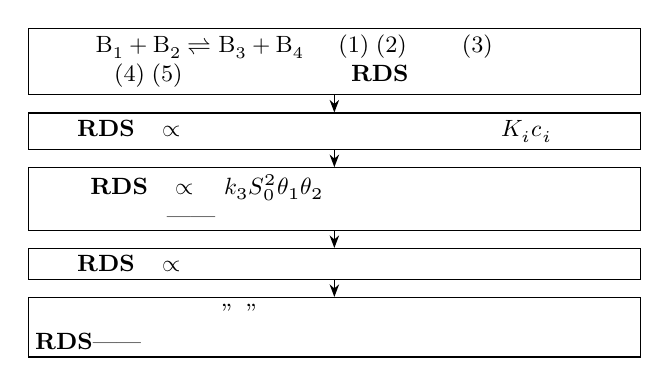
\begin{tikzpicture}[
  box/.style={draw, align=left, text width=76mm, inner sep=2.5pt,
              font=\fontsize{8.5}{10.5}\selectfont},
  ar/.style={-{Stealth[length=1.6mm]}, line width=0.6pt}
]
\node[box] (seq) {\textbf{五步基元序列}（以
$\mathrm{B_1+B_2\rightleftharpoons B_3+B_4}$ 为例）：(1)、(2) 反应物吸附；
(3) 相邻吸附物种的表面反应；(4)、(5) 产物脱附。稳态下各步净速率相等，
\textbf{最慢的一步即 RDS}，其余各步处于吸附平衡或化学平衡};
\node[box, below=2.2mm of seq] (ads) {\textbf{① 吸附为 RDS}：速率 $\propto$ 该组分的
吸附速率；分母中\textbf{缺少该组分的吸附项}（它尚未建立平衡），其余物种的覆盖度仍由
各自的 $K_ic_i$ 给出};
\node[box, below=2.2mm of ads] (srf) {\textbf{② 表面反应为 RDS}：速率
$\propto k_3S_0^2\theta_1\theta_2$；分母是\textbf{全部物种吸附项的完整多项式}，指数的
大小由「两物种是否竞争同一种吸附位」决定——同一吸附位取平方，两套独立吸附位则取两个
一次因子之积};
\node[box, below=2.2mm of srf] (des) {\textbf{③ 脱附为 RDS}：速率 $\propto$ 产物脱附
速率；分母中\textbf{缺少该产物的吸附项}，而\textbf{产物在表面上的覆盖度由前置平衡
（表面反应）决定}，因此方程中出现的是产物与反应物的分压比};
\node[box, below=2.2mm of des] (chk) {\textbf{判别线索}：①与③形式相近而分子推动力项
不同；②的分母最"完整"。三种形式在数学上互相接近，\textbf{因此只靠一组速率数据往往
无法唯一确定 RDS}——需借助初速度法、温度依赖性检验与独立吸附数据交叉判别};
\draw[ar] (seq)--(ads);
\draw[ar] (ads)--(srf);
\draw[ar] (srf)--(des);
\draw[ar] (des)--(chk);
\end{tikzpicture}
\caption{速率控制步骤（RDS）判别逻辑链：吸附、表面反应、脱附分别为 RDS 时速率方程形式的
差异。读者应看三处分母：缺少哪一项、多项式是否完整、指数的来源是什么。本图只给出形式
差异的定性骨架，不定量；三种形式在有限精度数据上可能互相近似，RDS 的最终判定需要
温度依赖性与独立吸附数据（见 §\ref{sssec:power-vs-hyp}）。
\schemamark\figsrc{据 S2（下册）§10.2.2—§10.2.3，书内 p.753—756 / PDF p.242—245 的
式(10-63)、式(10-67)、式(10-68) 讨论绘制；非原书插图（原书图 10-1 为反应器示意）。}}
\label{fig:rds-chain}
\end{figure}

\paragraph{替代思路：最丰富反应中间物（MARI）。}「只有一个 RDS」是一个很强的假设。当几个
步骤的速率相当时，可以采用另一个视角：设表面上\textbf{最丰富反应中间物（most abundant
reaction intermediate，MARI）}占据几乎全部活性位，其余物种的覆盖度由与 MARI 之间的平衡
关系给出，于是表面上复杂的多步序列可被简化或等效为\textbf{两步反应}，仍能推出可用形式
的动力学方程，只是其中参数的物理意义已不同于均匀表面模型下的同名参数。
\src{S2 §10.3.5，书内 p.768 / PDF p.257} RDS 假设与 MARI 假设给出的方程形式常相同或相近，
两者真正的差别在于\textbf{哪一个覆盖度被当作由平衡决定}；这一路线的完整形式与模型判别
准则见后续分片。

\sloppy
\subsubsection{双曲线式速率方程（L-H 型）}

以理想表面为基础的动力学方程，要点是用表面覆盖度 $\theta$ 表达反应速率，再用 Langmuir
方程把 $\theta$ 与流体相浓度关联。这一表达方式由 Hinshelwood 提出，称 Langmuir-Hinshelwood
方法；Hougen 与 Watson 又引入空吸附位的概念，故也称 Hougen-Watson 方法；因形式无实质
改变，常合称 L-H 或 L-H-W 方法。\src{S2 §10.2.3，书内 p.754 / PDF p.243}

\begin{principle}
\textbf{从吸附平衡推出双曲线式速率方程——推导主线。}设总包反应
$\mathrm{B_1+B_2\rightleftharpoons B_3+B_4}$ 的基元序列为（$\mathrm{L}$ 为吸附位）：
(1) $\mathrm{B_1+L\rightleftharpoons B_1{\cdot}L}$；(2)
$\mathrm{B_2+L\rightleftharpoons B_2{\cdot}L}$；(3)
$\mathrm{B_1{\cdot}L+B_2{\cdot}L\rightleftharpoons B_3{\cdot}L+B_4{\cdot}L}$；
(4) $\mathrm{B_3{\cdot}L\rightleftharpoons B_3+L}$；(5)
$\mathrm{B_4{\cdot}L\rightleftharpoons B_4+L}$。设第 (3) 步为 RDS，其余四步处于吸附平衡。

\textbf{第一步：位平衡记账。}令 $S_0$ 为活性位密度，$\theta_i$ 与 $\theta_{\mathrm v}$ 为
吸附物种与空位的覆盖度。每个处于平衡的吸附步给出 $\theta_i=K_ic_i\theta_{\mathrm v}$，
代入 $\sum_i\theta_i+\theta_{\mathrm v}=1$ 得
\begin{equation}
\theta_{\mathrm v}=\frac{1}{D},
\qquad D=1+K_1c_1+K_2c_2+K_4c_3+K_5c_4
\label{eq:lh-D}
\end{equation}

\textbf{第二步：只写 RDS 的速率}（两个相邻吸附物种的表面反应，正逆各一项）：
\begin{equation}
r=k_3S_0^2\,\theta_1\theta_2-k_{-3}S_0^2\,\theta_3\theta_4
\label{eq:lh-rds}
\end{equation}

\textbf{第三步：把 $\theta$ 换成 $c$}（把 $\theta_i=K_ic_i\theta_{\mathrm v}$ 代入并合并）：
\begin{equation}
\begin{split}
r&=\frac{k_3K_1K_2S_0^2\left(c_1c_2-c_3c_4/K_0\right)}{D^2},\\
K_0&=\frac{k_3K_1K_2}{k_{-3}K_4K_5}=K_{\mathrm{eq}}
\end{split}
\label{eq:lh}
\end{equation}
式中 $k_3$ 为第 (3) 步的正向速率常数，$K_i$ 为第 $i$ 步的吸附平衡常数，$c_i$ 为气相浓度
（或分压），$K_{\mathrm{eq}}$ 为总包反应的化学平衡常数。\textbf{自检}：令 $r=0$，式
~\eqref{eq:lh} 自动回到总包反应的平衡式，这就是\textbf{热力学一致性}——任何按此路线推得
的速率方程都必须通过这一自检。
\end{principle}

\tocheck{未对照原页面图像：原书式(10-63) 后给出的 $K_0$ 定义（OCR 作
$K_{\mathrm{eq}}(K_1/K_2)K_4K_5$）与上述自洽推导得到的 $K_0=K_{\mathrm{eq}}$ 不一致；
此处按「$r=0$ 必须给出总包平衡式」这一硬约束重建。}

\textbf{量纲检查。}若 $c$ 取 $\mathrm{mol{\cdot}m^{-3}}$、$S_0$ 取
$\mathrm{mol{\cdot}m^{-2}}$、$\theta$ 无量纲，则 $K_i$ 为 $\mathrm{m^3{\cdot}mol^{-1}}$，
$k_3$ 为 $\mathrm{m^{2}{\cdot}mol^{-1}{\cdot}s^{-1}}$，$r$ 为
$\mathrm{mol{\cdot}m^{-2}{\cdot}s^{-1}}$（以单位活性面积为基准）。换成「以分压为浓度基准、
以催化剂质量为反应空间基准」时，$k_3$ 与 $S_0$ 会以不同方式并入表观常数，\textbf{这正是
同一条机理在不同文献中 $k$ 数值与量纲不同的原因}。

\textbf{通式与特例。}式~\eqref{eq:lh} 对以两种吸附反应物起表面反应为 RDS 的体系是通式，
几种重要特例列于下（均设不可逆或逆项可忽略）：
\begin{itemize}
\item 各组分均弱吸附（$K_ic_i\ll1$，$D\approx1$）：
$r\approx k(c_1c_2-c_3c_4/K_0)$，形式回到幂式（总级数 2）；若为单分子不可逆反应，
则退化为一级式 $r=kc_1$。
\item 产物 $\mathrm{B_3}$ 强吸附而反应物弱吸附（$K_4c_3\gg1\gg K_1c_1,K_2c_2$）：
$r\approx k\,c_1c_2/c_3$；单组分时 $r\approx k\,c_1/c_3$，即\textbf{产物抑制}型。
\item 反应物强吸附而产物弱吸附：$D\approx K_1c_1$，$r\approx k$，
即\textbf{零级反应}——这是「表面已被饱和」的动力学签名。
\end{itemize}
\src{S2 §10.2.3，书内 p.754—755 / PDF p.243—244，式(10-64)—(10-66)}

\textbf{分母指数从何而来。}式~\eqref{eq:lh} 分母的指数为 2，只适用于两种吸附物在
\textbf{同一种}吸附位上竞争吸附的情形；若 $\mathrm{B_1}$ 与 $\mathrm{B_2}$ 独立地分别吸附
在两种吸附位上，分母中相应的吸附项应改为 $(1+K_1c_1)(1+K_2c_2)$。此外，若机理设定为
\textbf{一个气相分子与一个吸附物种直接反应}（Rideal-Eley 机理），仍以 Langmuir 方程为
基础，所得速率方程形式相似，但分母上吸附项的指数为 1。
\src{S2 §10.2.3，书内 p.755 / PDF p.244}

\textbf{氧化-还原（Mars-van Krevelen）机理。}Rideal-Eley 机理有一个变体，由 Mars 与
van Krevelen 提出，用于烃类氧化反应：气相烃分子与催化剂表面晶格氧（或吸附氧）反应，
产物脱附，被还原的活性位再由气相氧重新氧化。按 Bodenstein 稳态原则
（$\dd[\mathrm{B_2{\cdot}L}]/\dd t=\dd[\mathrm{B_3{\cdot}L}]/\dd t=0$）并令各表面浓度分数
之和为 1，可得速率方程；若除产物脱附外其余各步不可逆，则化为
\begin{equation}
r=\frac{k_1k_2k_3c_1c_2}{k_1k_3c_1c_2+\nu_0k_2k_3c_2+k_1k_2c_1+k_1k_{-2}c_1c_3}
\label{eq:mvk}
\end{equation}
式中 $\nu_0$ 为计量数（烃分子常需数个晶格氧与之作用）。\textbf{注意分母的结构与
式~\eqref{eq:lh} 完全不同}：它不是覆盖度多项式，而是\textbf{各步速率常数之积的和}。
式~\eqref{eq:lh}、式~\eqref{eq:mvk} 一类方程都属\textbf{双曲线式}，其中包含多个参数，
适应性很广——\textbf{也正因为参数多，同一组动力学数据用不同机理（不同 RDS）的速率方程
拟合都可能得到满意结果}。\src{S2 §10.2.3，书内 p.755—756 / PDF p.244—245，
式(10-69)—(10-71)}

\begin{pitfall}
\textbf{「拟合得好」不是机理证据。}双曲线式方程参数多、形式灵活，一组数据（例如
$\mathrm{B_1+B_2\rightleftharpoons B_3+B_4}$ 的可逆反应）在吸附控速、表面反应控速、脱附控速
三种假设下都可能拟合得不错。要区分它们，至少需要：不同温度下的参数温度系数是否合理
（速率常数为正温度系数、吸附平衡常数为负温度系数）、由吸附平衡常数经 van't Hoff 关系
求得的吸附焓是否为负、以及独立测得的吸附数据是否支持所设的覆盖度范围。判据与模型检验
流程见后续分片。
\end{pitfall}

\textbf{积分表达式。}式~\eqref{eq:lh} 等均为微分表达式，把它与连续性方程结合积分即得积分
表达式，表达空时与转化率（或生成率）的关系。以单组元不可逆表面反应控速为例
（$\mathrm{B_1}\to\mathrm{B_2}$，$r=kS_0K_1p_1/(1+K_1p_1)$），代入活塞流积分式后可得
\begin{equation}
\frac{W}{F}\cdot\frac{S_0K_1p}{n_{\mathrm t0}}\,k
=\ln\frac{1}{1-X}+K_1pX
\label{eq:lh-int}
\end{equation}
\tocheck{未对照原页面图像：式~\eqref{eq:lh-int} 中 $n_{\mathrm t0}$ 因子与 $p$ 的定义
（总压还是 $\mathrm{B_1}$ 起始分压）无法从 OCR 确认；本式按「定容、$p_1=p(1-X)$、
$r=kS_0K_1p_1/(1+K_1p_1)$」自洽推导给出，与 OCR 相差可能只是一个常数因子。
}\textbf{式~\eqref{eq:lh-int} 与一级反应的式~\eqref{eq:pfr-int1} 的差别本身就是判据}：把
实验数据按 $\ln[1/(1-X)]$ 对 $W/F$ 作图，若得到通过原点的直线则与一级幂式一致；若需
附加 $K_1pX$ 项才成直线，则支持表面反应控速的 L-H 形式。更复杂的微分表达式一般无解析
积分，只能数值积分。\src{S2 §10.2.3，书内 p.756—757 / PDF p.245—246，式(10-72)、式(10-73)}

\subsubsection{表观活化能为何不等于真实活化能}
\label{sssec:eapp}

\begin{principle}
\textbf{表观活化能的分解。}双曲线式速率方程中的表观速率常数是「真实速率常数」与若干
吸附平衡常数的乘积或商。按 van't Hoff 关系 $K_i=K_i^{0}\exp(-\Delta H_{\mathrm{ads},i}/RT)$
（吸附放热，$\Delta H_{\mathrm{ads},i}<0$），由式~\eqref{eq:eapp-def} 可得
\begin{equation}
E_{\mathrm{app}}=E_{\text{真实}}+\sum_i \nu_i\,\Delta H_{\mathrm{ads},i}
\label{eq:eapp}
\end{equation}
式中 $\nu_i$ 为 RDS 速率表达式中组分 $i$ 的吸附平衡常数所带的指数（含正负号：在分子中取
正、在分母中取负）。\textbf{因此在一般情况下 $E_{\mathrm{app}}\neq E_{\text{真实}}$，
表观值中混入了吸附热的贡献}，且因为吸附是放热的，$\Delta H_{\mathrm{ads}}<0$。
\end{principle}

由式~\eqref{eq:lh} 的三种特例可以具体看出这一点（以表面反应为 RDS）：

\begin{itemize}
\item \textbf{低覆盖度}（$D\approx1$，$r\approx k_3K_1K_2S_0^2c_1c_2$）：
$E_{\mathrm{app}}=E_3+\Delta H_{\mathrm{ads},1}+\Delta H_{\mathrm{ads},2}$，
两种反应物的吸附热都进入表观值。
\item \textbf{$\mathrm{B_1}$ 强吸附}（$D\approx K_1c_1$，
$r\approx k_3K_2S_0^2c_2/(K_1c_1)$）：
$E_{\mathrm{app}}=E_3+\Delta H_{\mathrm{ads},2}-\Delta H_{\mathrm{ads},1}$，
强吸附组分的吸附热以\textbf{负}号进入。
\item \textbf{产物强吸附}（$D\approx K_4c_3$）：
$E_{\mathrm{app}}=E_3+\Delta H_{\mathrm{ads},1}+\Delta H_{\mathrm{ads},2}-2\Delta H_{\mathrm{ads},4}$，
产物吸附热以两倍权重被扣除。
\end{itemize}

\textbf{覆盖度变化使表观活化能本身成为温度的函数。}覆盖度 $\theta$ 由温度和各分压共同
决定：升温会降低 $K_i$（放热吸附），从而改变 $D$ 中哪一项占优，于是式~\eqref{eq:eapp}
中的有效 $\nu_i$ 组合在升温过程中发生切换。此时 Arrhenius 图不再是直线，而是\textbf{在
不同温度区间呈现不同斜率的弯曲曲线}（图~\ref{fig:arrh-bend}），而按式~\eqref{eq:eapp-def}
测得的只是该区间的局部斜率。

\begin{figure}[htbp]
\centering
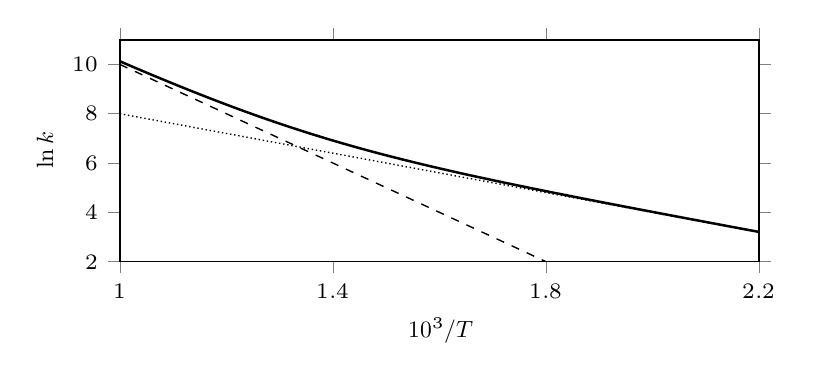
\begin{tikzpicture}
\tikzset{declare function={syn(\x)=ln(exp(20-10*\x)+exp(12-4*\x));
  lowE(\x)=20-10*\x; highE(\x)=12-4*\x;}}
\begin{axis}[
  width=\onecolwidth, height=44mm,
  xmin=1.0, xmax=2.2, ymin=2, ymax=11,
  xtick={1.0,1.4,1.8,2.2}, ytick={2,4,6,8,10},
  xlabel={$10^{3}/T$}, ylabel={$\ln k$}]
\addplot[domain=1.0:2.2,samples=160,mainline,black]{syn(x)};
\addplot[domain=1.0:1.8,samples=2,thinline,black,dashed]{lowE(x)};
\addplot[domain=1.0:2.2,samples=2,thinline,black,densely dotted]{highE(x)};
\end{axis}
\end{tikzpicture}
\caption{表观活化能随温度区间变化的模型 Arrhenius 图。读者应看两处：曲线在中段发生弯曲，
两侧渐近于两条不同斜率的直线（虚线、点线，斜率对应模型设定的 $E/R=10^{4}$ K 与
$4\times10^{3}$ K）；因此「表观活化能」只在单一渐近区才有确定数值。局限：本曲线由
$k=k_1+k_2$ 的两个并联通道合成，是覆盖度或控制步骤随温度切换的最小模型，不代表任何具体
反应，也不给出真实活化能的数值。\modelmark\figsrc{模型计算，依据 S2（下册）§10.2.3 与
§10.3.4 关于参数温度系数、Arrhenius 图不呈直线的讨论，书内 p.754—756、p.766—767 /
PDF p.243—245、p.255—256。}}
\label{fig:arrh-bend}
\end{figure}

\begin{keycond}
\textbf{读表观活化能时的四条边界。}（1）\textbf{RDS 随温度转移}同样造成弯曲：低温下表面
反应可能最慢，升温后吸附或脱附成为最慢步，Arrhenius 图出现折点。因此「Arrhenius 图不呈
直线」本身就是机理可能切换的证据，不应一律当作实验误差。（2）\textbf{接近化学平衡}时，
净速率中的推动力项 $(1-\beta)$（$\beta$ 为反应商与平衡常数之比）也带温度依赖并含总包
反应热，使净速率的表观活化能进一步偏离正向步骤的真实活化能；故动力学参数应在\textbf{远离
平衡}的转化率区间测定，或明确说明距平衡多远。（3）某些吸附是\textbf{吸热}的（例如 NO 在
催化剂上的吸附），此时吸附平衡常数具有正的温度系数、吸附焓为正值，式~\eqref{eq:eapp} 的
符号讨论要相应调整——「吸附必放热」是经验倾向而不是定律。（4）由 $K_i$ 经 van't Hoff
关系求得的吸附焓与吸附熵都应为负值；这是模型参数能否成立的物理判据，但\emph{其置信区间
常很宽，单点估值为负不足以立刻否定一个模型}——用线性回归得到负值、用非线性回归却得到
正值的例子并不罕见。判据的完整清单、回归方法与模型判别流程见后续分片。
\src{S2 §10.3.4，书内 p.766—767 / PDF p.255—256}
\end{keycond}

\subsubsection{幂式速率方程及其适用边界}
\label{sssec:power-vs-hyp}

幂式速率方程在多相催化动力学中同样经常被使用。对可逆反应，其通式为
\begin{equation}
r=k_1\prod_i c_i^{m_i}-k_{-1}\prod_i c_i^{n_i}
\label{eq:power-rev}
\end{equation}
式中 $m_i$、$n_i$ 可为正数或负数，也可为整数或分数。
\src{S2 §10.2.4，书内 p.757 / PDF p.246，式(10-74)}

\textbf{氨合成是最著名的例子。}其普适动力学速率方程写作
\begin{equation}
r=k_1\,p_{\mathrm{N_2}}p_{\mathrm{H_2}}^{3\alpha}p_{\mathrm{NH_3}}^{-2\alpha}
-k_{-1}\,p_{\mathrm{NH_3}}^{2(1-\alpha)}p_{\mathrm{H_2}}^{-3(1-\alpha)}
\label{eq:ammonia}
\end{equation}
式中 $k_1$、$k_{-1}$ 为与解离吸附、脱附相联系的速率常数，$\alpha$ 为 Temkin 常数，取值在
$0$ 与 $1$ 之间、通常为 $0.5$。该式可由 $\mathrm{N_2}$ 解离吸附控速机理出发、以 Temkin
吸附等温方程为基础导出；实验数据符合式~\eqref{eq:ammonia}，说明该反应属于
$\mathrm{N_2}$ 解离吸附控速的机理。\src{S2 §10.2.4，书内 p.757 / PDF p.246，式(10-75)}

\begin{principle}
\textbf{幂式方程的热力学一致性自检。}令式~\eqref{eq:ammonia} 的 $r=0$，得
\begin{equation}
\frac{p_{\mathrm{N_2}}p_{\mathrm{H_2}}^{3}}{p_{\mathrm{NH_3}}^{2}}
=\frac{k_{-1}}{k_1}=\frac{1}{K_{\mathrm{eq}}}
\label{eq:ammonia-eq}
\end{equation}
即速率方程在 $r=0$ 时自动还原为化学平衡式。\textbf{任何幂式方程都必须通过这一自检}，
否则它连平衡位置都算不对，不能用于接近平衡的过程模拟。
\tocheck{未对照原页面图像：OCR 把该平衡关系写作 $=k_1/k_{-1}=1/K$，与令 $r=0$ 的自洽结果
（式~\eqref{eq:ammonia-eq}）互为倒数，此处按自洽结果给出。}
\end{principle}

\textbf{幂式方程并不只是经验拟合，它也能从机理推出。}两条路线都成立，且都赋予级数物理
含义。

\textbf{路线一（非均匀表面，基于 Freundlich 方程）。}推导分三步：写出 RDS 的速率式（其中
$\theta$ 以幂次出现）；用 Freundlich 方程把 $\theta$ 换成该物种的「有效分压」
$p_{i\mathrm e}$；再用表面的化学平衡关系把 $p_{i\mathrm e}$ 换成气相分压。以单分子反应
$\mathrm{B_1}\to\mathrm{B_2}$（$\mathrm{B_1}$ 吸附强于 $\mathrm{B_2}$）为例，若
\textbf{表面反应为 RDS}，则 $\theta_1=(p_{1\mathrm e}/p_{1\mathrm s})^{1/n_1}$，
$r=k_2\theta_1^{m_1}=k_2(p_{1\mathrm e}/p_{1\mathrm s})^{m_1/n_1}=k'p_1^{m_2}$，其中
$m_2=m_1/n_1$——形式仍是幂式，但级数由吸附等温线的指数 $n_1$ 与反应级数 $m_1$ 共同决定。
吸附为 RDS 或脱附为 RDS 时同法可得形式上仍是幂式、但级数组合与相应平衡关系挂钩的方程。
\tocheck{未对照原页面图像：式(10-78)—(10-81) 中「吸附控速」与「脱附控速」两式的级数组合
（OCR 作 $r=kp_1/p_2^{m_2}$ 一类）无法确认，此处只保留可由 $r=k_2\theta_1^{m_1}$ 自检的
表面反应控速一式，其余只给推导路线。}以 Freundlich 方程为基础，可以推出与一定 RDS 相应的
氨合成、氨分解、正仲氢转换、一氧化碳氧化及乙烷氢解等反应的幂式速率方程；Kwan 系统讨论了
以 Freundlich 方程为基础、不同控速步骤得出的不同动力学方程，并指出很多化学吸附系统的
吸附-脱附速率在较宽压力范围内既可用幂式方程也可用 Freundlich 方程表达。
\src{S2 §10.2.4，书内 p.757—758 / PDF p.246—247}

\textbf{路线二（理想均匀表面，基于 Langmuir 方程）。}设双组元反应
$\mathrm{B_1+B_2}\to\mathrm{B_3}$ 通过中间表面络合物 $\mathrm{B_1{\cdot}L}$ 的生成与分解
进行，$\mathrm{B_1}$ 的覆盖度按 Langmuir 方程为
$\theta_1=K_1p_1/(K_1p_1+K_2p_2)$，则速率方程为 $r=kp_1^{m_1}p_2^{m_2}$，其中

\begin{equation}
\begin{split}
m_1&=\frac{K_2p_2}{K_1p_1+K_2p_2}=1-\theta_1,\\
m_2&=\frac{K_1p_1}{K_1p_1+K_2p_2}=\theta_1,
\qquad m_1+m_2=1
\end{split}
\label{eq:golodets}
\end{equation}
这解释了幂式方程中\textbf{级数为什么常是分数、为什么随分压漂移}：级数本身就是覆盖度的
函数，不是本征常数。该解析被用于化合物氧化反应，论证了水中毒（水蒸气中毒）效应、
$m_1+m_2$ 常为 $1$、以及级数与氧化物催化剂的氧键能、活化能和补偿效应之间的关联。
\src{S2 §10.2.4，书内 p.758—759 / PDF p.247—248，式(10-82)}

\begin{table}[htbp]
\centering
\caption{幂式与双曲线式速率方程的对照。读者应看两处：参数的含义（$m_i$ 是覆盖度的函数，
$K_i$ 有热力学约束）与外推风险的方向性差别。两者都能拟合同一套数据，选择依据应是外推
需求与参数的物理可解释性，而不是拟合残差的大小。\src{据 S2 §10.2.3—§10.2.4，书内
p.754—759 / PDF p.243—248 归纳。}}
\label{tab:power-vs-hyp}
{\srcsize
\begin{tabularx}{\columnwidth}{@{}lXX@{}}
\toprule
项目 & 幂式速率方程 & 双曲线式速率方程（L-H 型） \\
\midrule
吸附模型基础 & Freundlich（吸附焓 $\propto\ln\theta$，非均匀表面）& Langmuir（吸附焓与
$\theta$ 无关，均匀表面）\\
\addlinespace
一般形式 & $r=k\prod_i c_i^{m_i}$ & $r=k\times$（推动力项）$/$（吸附项多项式）\\
\addlinespace
参数含义 & $k$ 为表观速率常数；$m_i$ 为表观级数，可正可负、可整数可分数，且\textbf{本身
是温度和覆盖度的函数} & $k$ 含真实速率常数与吸附平衡常数之积；$K_i$ 有明确热力学约束
（放热、$\Delta S_{\mathrm{ads}}<0$）\\
\addlinespace
适用场景 & 分压范围宽、覆盖度变化大；产物分压不过低；工程关联与放大初算 & 需要机理含义、
需要向其他温度或组成外推；有独立吸附数据可支持所设的覆盖度范围\\
\addlinespace
外推风险 & \textbf{高}：级数非本征量，跨温度区间外推时级数会漂移；含负级数的项在相应
分压趋于零时发散 & \textbf{中}：形式可外推，但参数多、相关性强，同一数据常有多套参数
给出同样好的拟合\\
\addlinespace
与机理的关系 & 可由 Freundlich／Temkin 或 Langmuir 基础推出，也可纯经验拟合 & 有明确
机理假设；但吸附控速、表面反应控速、脱附控速三种假设常都能拟合同一数据\\
\bottomrule
\end{tabularx}}
\end{table}

\begin{pitfall}
\textbf{幂式方程的外推是本章最容易出事的一步。}（1）把 $m_i$ 当作与温度无关的常数、跨
温度区间外推没有根据：由式~\eqref{eq:golodets}，$m_i$ 是覆盖度的函数，而覆盖度随温度
变化；幂式回归所得级数随温度「有相当变迁」、因而求不出稳定的表观活化能，正是这一原因。
（2）含\textbf{负级数}的项（如式~\eqref{eq:ammonia} 中的 $p_{\mathrm{NH_3}}^{-2\alpha}$）
在相应分压趋于零时发散，\textbf{不可外推到该组分分压很低的区间}。（3）幂式方程形式单一、
数学处理一般只有唯一解，容易让人误以为「参数唯一就代表机理唯一」；实际上幂式方程同样可被
多个机理导出，参数的正负与整分性只是线索，不是证明。（4）幂式方程的积分表达式一般比双
曲线式的更难有解析解：简单情形可化为式(10-39)、式(10-41) 的形式，复杂时只能数值积分，
此时参数误差与数值积分误差会叠加。\src{S2 §10.2.4，书内 p.757 / PDF p.246}
\end{pitfall}

\begin{crosscheck}
\textbf{与本章其他分片及其他章的回查关系。}（1）本分片两次用到吸附等温方程
（式~\eqref{eq:langmuir-ch10}、式~\eqref{eq:langmuir-diss} 以及 Freundlich／Temkin 方程）：
\textbf{Langmuir 方程的推导、三条基本假定及其适用窗口已在\chapref{ch:01}给出，此处直接
引用}；当数据明显偏离 Langmuir（吸附焓随覆盖度变化）时，应回到\chapref{ch:01}核对模型
选择，而不是强行用双曲线式拟合。（2）TOF 的分母——活性位数 $S$——来自化学吸附滴定，其
测量方法与化学计量比的验证见\chapref{ch:05}；\textbf{没有独立的活性位计数，任何 TOF 数值
都只是「每克催化剂的速率」的另一种写法}。（3）速率方程中的吸附平衡常数若要独立验证，
需要变温吸附或程序升温脱附数据；只有动力学数据本身时，$K_i$ 与其置信区间必须一并报告。
（4）模型检验、微分／积分数据处理、线性与非线性回归、判别准则与非均匀表面动力学属于
后续分片；本分片给出的每一类方程都是它们的数据来源形式。
\end{crosscheck}

\begin{methodsum}
\textbf{本分片建立的流程（四步）。}（1）\textbf{确定可测定义}：化学计量方程式~\eqref{eq:stoi}
$\to$ 反应度式~\eqref{eq:xi} $\to$ 速率式~\eqref{eq:rate-def}，同时声明 $Q$ 基准与转化率
测量点。（2）\textbf{选反应器模型}：微分数据用 CSTR 的代数式~\eqref{eq:cstr}；积分数据用
PFR 的式~\eqref{eq:pfr} 及其积分式~\eqref{eq:pfr-int1}，并核对等温、无返混、无传递限制
三条边界。（3）\textbf{设 RDS 并写速率方程}：按「只写 RDS 速率 $+$ 其余步骤取平衡」的规则
推出双曲线式式~\eqref{eq:lh}；若表面非均匀或需宽分压范围关联，则用幂式
式~\eqref{eq:power-rev}。（4）\textbf{做三项自检}：$r=0$ 是否回到平衡式（热力学一致性）；
参数的温度系数与符号是否合理；表观活化能是否因覆盖度或 RDS 转移而弯曲（§\ref{sssec:eapp}）。
报告时至少给出：速率方程形式、$Q$ 基准、温度区间、转化率区间、参数值与置信区间。
\end{methodsum}
}{}
\IfFileExists{chapters/parts/ch10-b.tex}{% ================================================================
%  chapters/parts/ch10-b.tex
%  第 10 章  多相催化反应动力学（分片 b）
%  源：S2（下册）第 10 章，书内 p.769—792 / PDF p.258—281
%  覆盖：10.3 动力学模型的建立与检验；10.4 多相催化中的传递过程
%  说明：分片 a 写 10.1—10.2，分片 c 写 10.5—10.6。本分片不含 \chapterstart。
%        所有公式按「OCR 上下文 + 学科标准形式」重建，未对照原页面图像；
%        存疑处一律就地标 \tocheck{}。
% ================================================================

\subsection{动力学模型的建立与检验}
\label{sec:ch10-model}

前两节给出了速率方程的各种形式和判断速率控制步骤的方法。但从一组实验数据到一个可以
外推的速率方程，中间还有三步工作：定候选模型族、估参数、判定「这个模型能不能用」。
本节做这三步，并讲清一句常被含糊过去的话——\textbf{拟合优度高不等于模型正确}。

\begin{probout}
（1）面对同一组「速率—组成」数据，幂式、L-H 式、非均匀表面的 Temkin 式在数据窗口内
可能几乎重合，凭什么选一个？（2）参数估出来以后，怎么判断它\textbf{物理上合理}，而不
只是数学上的一组数字？（3）残差图该看什么——「残差小」与「残差随机」是两回事；
（4）什么条件下两个模型\textbf{原则上不可能}被这组数据区分（可辨识性），此时继续比较
$R^2$ 等于在比较噪声。本节还要交代一件更少被提及的事：\textbf{估计参数所用的数据窗口
本身决定了参数的含义}——同一个模型、同一套数据，只换窗口，表观级数就会变。
\end{probout}

\subsubsection{模型族：从幂式到非均匀表面}

催化剂动力学模型分三个层次，混用层次是很多错误的起点。\textbf{幂式}
$r=kp^n$ 是\textbf{纯经验的插值式}：$n$ 不是机理量，它只保证在实测窗口内可用；
\textbf{双曲线式（L-H 型）}由吸附平衡加一个速率控制步骤推出，参数有明确含义
（吸附平衡常数 $K$、表面速率常数 $k_S$），可外推到未测的组成；\textbf{非均匀表面模型}
再往前走一步，不假定所有活性位等价，而是给出一套吸附势分布。前两节的 L-H 式与
M-vK 式属于第二层，下面补上第三层。

\begin{principle}
\textbf{非均匀表面（Temkin）模型的基本假定}\src{S2 §10.3，书内 p.769 / PDF p.258}：
（1）活性位的标准吸附势 $A_0$ 有连续分布函数
$\dd S'=a\exp(-\gamma A_0/RT)\,\dd(A_0/RT)$，$\gamma$ 为分布特征参数，$a$ 为归一化因子，
$\dd S'$ 是标准吸附势落在 $A_0$ 与 $A_0+\dd A_0$ 之间的活性位数目；
（2）速率常数与平衡常数之间有 Br\"onsted 型关系 $k_i=cK_i^{\alpha}$，$\alpha$ 为
Temkin 系数，取值 $0$—$1$，通常为 $0.5$；
（3）化学上类似的两个步骤（吸附与脱附）的变换系数相同；
（4）覆盖度 $t$ 的上限是全部活性位被占，下限是全部活性位空着。
\end{principle}

由这四条假定，可对两步反应 $\mathrm{S_1+A_1\rightleftharpoons B_1+S_2}$、
$\mathrm{S_2+A_2\rightleftharpoons B_2+S_1}$ 导出非均匀表面上的速率式
\src{S2 §10.3，书内 p.769 / PDF p.258}：

\begin{equation}
v_t=\frac{v}{[L]}
=\tau\,
\frac{k_1^{\mathrm{o}}k_2^{\mathrm{o}}[A_1][A_2]-k_{-1}^{\mathrm{o}}k_{-2}^{\mathrm{o}}[B_1][B_2]}
{\bigl(k_1^{\mathrm{o}}[A_1]+k_{-2}^{\mathrm{o}}[B_2]\bigr)^{m}
 \bigl(k_{-1}^{\mathrm{o}}[B_1]+k_2^{\mathrm{o}}[A_2]\bigr)^{1-m}}
\label{eq:temkin}
\end{equation}

其中 $v/[L]$ 是单位活性位上的速率，$k_i^{\mathrm{o}}$ 为 $A_0=0$ 处的速率常数；
分布因子 $\tau$ 与指数 $m$ 由式 (10-99) 的后两行给出。
\tocheck{未对照原页面图像：式 (10-99) 中 $\tau$ 与 $m$ 的确切定义——OCR 只剩
$\pi/\sin(\pi m)$ 与 $\exp(\gamma f)-1$ 的残迹，$\exp(\gamma f)-1$ 在分子还是分母、
$m$ 与 $a$、$\gamma$、$f$ 的组合方式都无法从文字层确认；引用前请核对原页面。}

式~\eqref{eq:temkin} 真正值得看的是\textbf{结构}：分母是两个「吸附项之和」分别取 $m$ 与
$1-m$ 次幂。当某个物种的吸附项占优时，表观级数自动落在 $0$ 与 $1$ 之间连续变化——
这正是非均匀表面模型与 L-H 式在形式上的最大差别（L-H 式的幂次是整数，级数只能取
$1$、$0$、$-1$ 这些离散值）。原书指出，该式除由两步反应导出外，还得到铁基催化剂上
氨合成的总包动力学数据、氮气吸附等温线形式和氮吸附速率数据的支持。
\src{S2 §10.3，书内 p.769 / PDF p.258}

\begin{table}[htbp]
\centering
\caption{同一组数据上的四类候选速率方程：参数、可辨识条件与失效边界。
选取时应先看第 4 列——数据窗口是否覆盖了能把模型区分开的那段条件。
\src{据 S2 §10.2.2—§10.2.3（书内 p.753—756 / PDF p.242—245）、§10.2.4
（书内 p.757—759 / PDF p.246—248）、§10.3.5（书内 p.768—769 / PDF p.257—258）整理。}}
\label{tab:ch10-modelfam}
\begin{tabularx}{\textwidth}{@{}l l l X@{}}
\toprule
类型 & 速率方程（单组分，$p$ 为分压） & 参数 & 可辨识条件与失效边界 \\
\midrule
幂式 & $r=kp^{n}$ & $k,\ n$ & $n$ 是窗口的产物而非机理量（本节例：$n=0.50\to0.20$）；
只可在实测窗口内插值，不可外推到极值区 \\
L-H 单站 & $r=kKp/(1+Kp)^{2}$ & $k,\ K$ & 必须覆盖 $p\approx1/K$ 的极值区；$k$ 与 $K$
强相关时须由独立吸附数据定 $K$，否则两者只能定出乘积 \\
L-H 解离 & $r=k\sqrt{Kp}/(1+\sqrt{Kp})^{2}$ & $k,\ K$ & 窗口窄时与单站式\textbf{不可区分}
（$p\ll1/K$ 时两式都退化为一级） \\
非均匀表面 & 式~\eqref{eq:temkin} & $k_i^{\mathrm{o}},\ \gamma,\ m$ & 参数多，需要覆盖
吸附项主次互换的条件区；单一温度的数据无法定出分布参数 $\gamma$ \\
\bottomrule
\end{tabularx}
\end{table}

\subsubsection{参数估计：数据窗口决定参数的含义}

\textbf{先定反应器，再定转化率范围。}求取动力学参数的反应器按转化率分为两类
\src{S2 §10.5.1，书内 p.779—781 / PDF p.268—270}：\textbf{积分反应器}装填足量催化剂，
进出口组成差别显著，无法用某个平均值代表全床组成，得到的是\textbf{转化率对空时的积分
数据}，分析要求不高，但必须对模型作积分后才能与数据比较；\textbf{微分反应器}的转化率
很低，进出口浓度差小到可用平均值代表全床组成，于是 $\Delta c/\Delta t$ 可近似为
$\dd c/\dd t$ 并等于反应速率 $r$，直接得到「$r$ 对平均组成」的\textbf{微分数据}，
代价是分析精度要求很高，而且数据往往是初速，难以配出复杂反应在高转化下的组成
（对策是在微分反应器前串接一个积分转化器提供进料）。
单程流通的管式微分反应器中，\textbf{转化率应在 $5\%$ 以下（个别允许到 $10\%$）}。

\begin{measure}
\textbf{估参数之前要固定的四件事。}（1）\textbf{恒温}：温度对速率是指数的，任何温度
梯度都直接变成速率误差。（2）\textbf{接触时间确切}：接触时间不确定，模型就无法与数据
对齐。（3）\textbf{转化率范围}：微分数据要求 $X<5\%$（个别 $\le10\%$）；
\textbf{转化率超过约 $15\%$ 的数据不能用来求反应级数}——此时沿床层的组成变化太大，
「平均组成」不再代表反应发生时的组成，级数被系统性地推离真值（见下方误判块）。
（4）\textbf{独立条件数}：独立自变量（组成、温度）的个数必须多于待估参数个数；
温度点少于 $3$ 个时 Arrhenius 参数与指前因子无法分开。
\src{S2 §10.5.1，书内 p.779—781 / PDF p.268—270}
\end{measure}

\textbf{拟合的权重问题。}把 $r=kp^n$ 取对数化成直线再作最小二乘，是最常见的做法，但它
\textbf{把「对 $r$ 的等权拟合」偷换成了「对 $\ln r$ 的等权拟合」}：低速率点的相对误差被
放大，高速率点被压缩。差别在窗口宽时可达可观量级。稳妥做法是：用对数直线只求\textbf{初值}，
再用非线性最小二乘直接拟合 $r$（或拟合相对残差 $\delta_i=(r_i^{\mathrm{cal}}-r_i)/r_i$，
使各点权重与其精度相称）。

\textbf{参数相关性是估计阶段的主要风险。}在 $r=kKp/(1+Kp)^2$ 里，只要 $Kp\ll1$，
速率就退化为 $r\approx kKp$：$k$ 与 $K$ 只能定出乘积 $kK$，各自的值由数据的噪声决定。
表现是：$k$ 与 $K$ 的相关系数接近 $\pm1$、置信区间极宽、换一批数据两者一起大幅漂移。
诊断与处置：算参数的相关矩阵，$|\mathrm{corr}|>0.95$ 时不要把 $k$ 与 $K$ 分开解释；
用独立信息（吸附量、程序升温脱附得到的覆盖度、瞬态实验）钉住其中一个参数。

\begin{dataflow}
\textbf{从原始数据到速率方程（本例为微分数据）。}
（1）核对物料衡算：进出口流量、组成、催化剂质量与接触时间的闭合误差；
（2）换算基准：把分析得到的摩尔数变化换成\textbf{单位质量}速率 $r_m$，需要与判据比较时
再乘颗粒密度换成单位体积速率 $r_v=\rho_pr_m$（详见下一节）；
（3）作图与选窗口：先画 $r$ 对 $p$ 的全窗口图，确认有没有极值、有没有产物阻抑或传质
控制的迹象，再决定用哪一段窗口估参数；
（4）求初值：对数直线或文献值；
（5）非线性最小二乘，输出参数、参数相关系数矩阵、残差序列；
（6）\textbf{判据检查}：残差是否随机、参数是否落在物理允许范围、窗口外能否预测
（见下小节）。
\end{dataflow}

换窗口会怎样，可以用本节的教学设定数据直接量出来：数据按 L-H 模型
（$k=2.00$、$K=0.50$\,\unit{kPa^{-1}}）生成并叠加 $\pm1.5\%$ 的相对噪声，共 $9$ 个点，
$p=0.5$—$3.0$\,\unit{kPa}。用同一个幂式分别拟合三个窗口，结果见表~\ref{tab:ch10-window}。

\begin{table}[htbp]
\centering
\caption{同一套教学设定数据、同一个幂式模型，只换拟合窗口：幂式指数 $n$ 从 $0.50$ 漂到
$0.20$（变 $2.5$ 倍），而 L-H 的吸附平衡常数 $K$ 在三个窗口下都停在 $0.51$—$0.52$
（生成值 $0.50$）。\textbf{参数的窗口稳定性比 $R^2$ 更能判断模型是否可信。}
\src{表中数值为本改编本按 L-H 模型生成的教学设定数据，非源书实验值；拟合窗口与参数
可辨识性的讨论据 S2 §10.3.2—§10.3.3，书内 p.760—765 / PDF p.249—254 整理。}}
\label{tab:ch10-window}
\begin{tabularx}{\textwidth}{@{}l c c c c@{}}
\toprule
拟合窗口 $p$/\unit{kPa} & 点数 & 幂式指数 $n$ & 幂式 $R^{2}$ & L-H 的 $K$/\unit{kPa^{-1}} \\
\midrule
$0.5$—$0.9$ & 3 & $0.496$ & $0.995$ & $0.510$ \\
$0.5$—$1.5$ & 5 & $0.371$ & $0.963$ & $0.520$ \\
$0.5$—$3.0$ & 9 & $0.201$ & $0.723$ & $0.510$ \\
\bottomrule
\end{tabularx}
\end{table}

窄窗口内幂式的 $R^2$ 高达 $0.995$，残差只有 $\pm1\%$：\textbf{只看 $R^2$，两个模型在这
三个点上无法区分}。但同一模型换到宽窗口，指数就从 $0.50$ 掉到 $0.20$；而 L-H 的 $K$
不随窗口移动。\textbf{一个参数如果随拟合窗口漂移，它就不是机理量。}
\pedset{表~\ref{tab:ch10-window} 与本节全部残差、$R^2$ 数值均为按 L-H 模型生成的
教学设定数据，非原书实验值。}

\subsubsection{模型判别与残差分析}

残差不是「拟合剩下的垃圾」，它是模型与数据之间唯一的结构性信息。判别的顺序是：
\textbf{先看残差的结构，再看参数的物理合理性，最后才看拟合优度}。本节用同一套数据的
两个拟合来演示。

\begin{figure}[htbp]
\centering
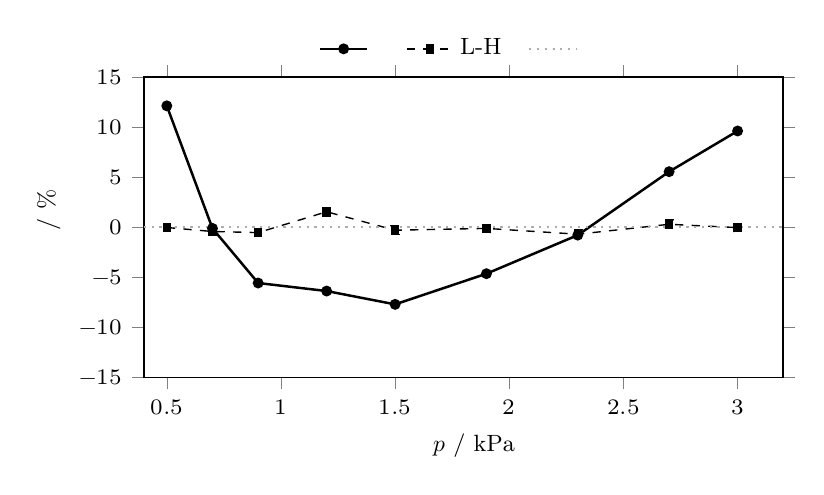
\begin{tikzpicture}
\begin{axis}[
  width=\onecolwidth,
  height=5.4cm,
  xlabel={分压 $p$ / \unit{kPa}},
  ylabel={相对残差 / \%},
  xmin=0.4, xmax=3.2, ymin=-15, ymax=15,
  xtick={0.5,1.0,1.5,2.0,2.5,3.0},
  ytick={-15,-10,-5,0,5,10,15},
  legend style={at={(0.5,1.02)}, anchor=south, legend columns=3, draw=none, fill=none},
]
\addplot[mainline, mark=*, mark size=1.5pt] coordinates {
  (0.50,12.11) (0.70,-0.12) (0.90,-5.57) (1.20,-6.37) (1.50,-7.70)
  (1.90,-4.64) (2.30,-0.79) (2.70,5.54) (3.00,9.60)};
\addlegendentry{幂式拟合}
\addplot[thinline, dashed, mark=square*, mark size=1.5pt] coordinates {
  (0.50,-0.03) (0.70,-0.43) (0.90,-0.54) (1.20,1.54) (1.50,-0.30)
  (1.90,-0.12) (2.30,-0.70) (2.70,0.29) (3.00,-0.04)};
\addlegendentry{L-H 拟合}
\addplot[accentsoft, dotted, thick] coordinates {(0.4,0)(3.2,0)};
\addlegendentry{零残差}
\end{axis}
\end{tikzpicture}
\caption{同一组数据、两种模型的相对残差随分压的分布。读图看两件事：幂式的残差
\textbf{符号成块}（$+,-,-,-,-,-,-,+,+$，连成一条弓形），L-H 的残差\textbf{符号交替}且
落在 $\pm1.6\%$ 内。条件与局限：数据为按 L-H 模型生成并加 $\pm1.5\%$ 相对噪声的教学
设定数据（$9$ 点，$p=0.5$—$3.0$\,\unit{kPa}），模型计算结果，不代表任何具体催化剂。
\modelmark}
\label{fig:ch10-resid}
\end{figure}

\begin{obs}
读图~\ref{fig:ch10-resid}：幂式拟合的残差在 $p=0.5$\,\unit{kPa} 处为 $+12.1\%$，随后
连续 $7$ 个点为负（$-0.1\%$、$-5.6\%$、$-6.4\%$、$-7.7\%$、$-4.6\%$、$-0.8\%$ 等），
在 $p>2.3$\,\unit{kPa} 又转为正（$+5.5\%$、$+9.6\%$）；符号序列为
$+,-,-,-,-,-,-,+,+$。L-H 拟合的 $9$ 个残差全部落在 $\pm1.6\%$ 以内，符号交替
（$-,+,-,-,-,-,+,-$），看不出结构。两个模型在同一组数据上的 $R^2$ 分别为
$0.723$ 与 $0.997$。
\end{obs}

\begin{infer}
（1）连续 $7$ 个同号残差不可能是噪声造成的：噪声在各点之间独立，不会成块同号。
\textbf{成块的残差是函数形式缺失的特征}——幂式在整段窗口里只有一个恒定斜率，而真实
速率曲线的斜率在变，误差于是按「两端正、中间负」的方式积累。（2）因此判别模型不能
用「残差小」或 $R^2$，要用\textbf{残差是否随机、是否与自变量或未进入模型的变量相关}。
（3）本例中 $R^2$ 恰好把错误模型暴露了（$0.723$ 对 $0.997$），但这是数据窗口的运气：
把窗口缩到表~\ref{tab:ch10-window} 的第一行（三个点），同一个幂式的 $R^2$ 就是
$0.995$、残差 $\pm1\%$——此时 $R^2$ 已经失去判别力。（4）残差随机只说明模型与这组
数据\textbf{相容}，不说明机理正确；机理结论必须另找独立证据（见本小节末的互补与回查）。
\end{infer}

\begin{table}[htbp]
\centering
\caption{残差图的形态与它提示的病因。这张表是判别阶段的检查清单：先按形态定位病因，
再决定是改模型、改权重还是去排除传递过程。
\src{本表为本改编本归纳的残差诊断清单，非源书表格；模型判别的准则据
S2 §10.3.4，书内 p.766—767 / PDF p.255—256。}}
\label{tab:ch10-resid-diag}
\begin{tabularx}{\textwidth}{@{}l X X@{}}
\toprule
残差形态 & 提示 & 处置 \\
\midrule
符号成块的连续弯曲 & 函数形式缺失（模型阶次或机理形式不对） & 换机理型模型；
扩宽条件窗口后重看残差 \\
残差与某个\textbf{未进入模型}的自变量相关（粒径、线速、空速） &
传递过程混入表观动力学 & 先按下一节的判据排除外扩散与内扩散，再重新拟合 \\
残差绝对值随速率增大 & 误差模型不对（等权拟合给了高值区过大权重） &
改用相对残差或加权最小二乘 \\
少数点残差远大于其余 & 离群点或分析误差 & 回查原始记录；不要为了 $R^2$ 删点 \\
残差随机但参数置信区间极宽、相关矩阵近奇异 & 数据信息量不足或参数强相关 &
补独立条件（更宽的分压、更多温度点、独立吸附量数据） \\
残差随机、参数稳定、窗口外可预测 & 与数据相容 & 仍不等于机理正确，需独立实验回查 \\
\bottomrule
\end{tabularx}
\end{table}

\textbf{「拟合优度高」为什么不能当判据。}三条理由，任一条都足以否掉用 $R^2$ 排模型优劣：
（1）$R^2$ 对\textbf{系统性偏差不敏感}——只要数据窗口窄、噪声大，错误模型也能拿到
$0.995$（表~\ref{tab:ch10-window} 第一行）；（2）$R^2$ 从不检查参数是否\textbf{物理
合理}，而 $k<0$、$K<0$、活化能为负的拟合在数值上完全可能；（3）增加参数\textbf{总能}
提高 $R^2$，所以参数个数不同的模型之间比 $R^2$ 是\textbf{过拟合的邀请函}——判据应是
「自由度 $n-p$ 下的残差是否与噪声量级一致」，而不是 $R^2$ 的大小。

\textbf{模型能否区分，取决于数据窗口。}把两个模型各自外推到数据窗口之外，差别才显现
（图~\ref{fig:ch10-extrap}）：幂式在 $p=8$\,\unit{kPa} 给出 $0.635$，比窗口内的最大值还
高；L-H 给出 $0.319$，并已越过 $p\approx2$\,\unit{kPa} 的极大值开始下降。实验数据在
$p>2$\,\unit{kPa} 确实下降，所以\textbf{幂式的函数形式在物理上已被否掉}——尽管它在
$0.5$—$0.9$\,\unit{kPa} 内 $R^2=0.995$。

\begin{figure}[htbp]
\centering
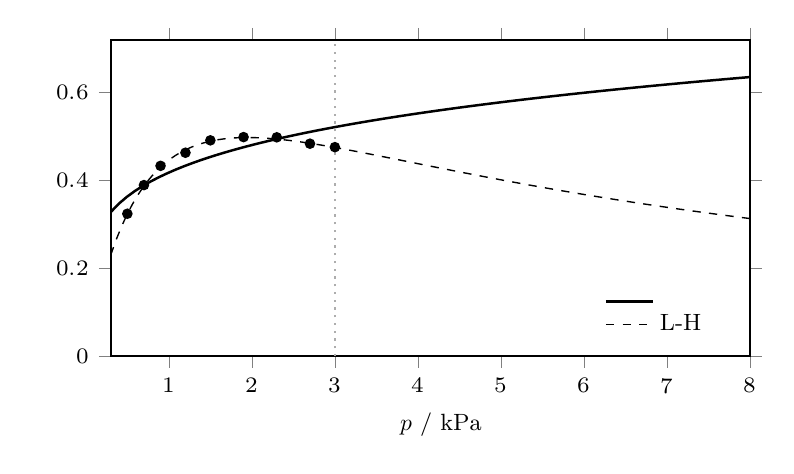
\begin{tikzpicture}
\begin{axis}[
  width=\onecolwidth,
  height=5.6cm,
  xlabel={分压 $p$ / \unit{kPa}},
  ylabel={相对速率（任意单位）},
  xmin=0.3, xmax=8.0, ymin=0, ymax=0.72,
  legend style={at={(0.98,0.03)}, anchor=south east, draw=none, fill=none},
]
\addplot[only marks, mark=*, mark size=1.6pt, forget plot] coordinates {
  (0.50,0.3241) (0.70,0.3893) (0.90,0.4331) (1.20,0.4629) (1.50,0.4911)
  (1.90,0.4985) (2.30,0.4980) (2.70,0.4835) (3.00,0.4756)};
\addplot[mainline, domain=0.3:8.0, samples=80]{0.4178*x^0.2014};
\addlegendentry{幂式外推}
\addplot[thinline, dashed, domain=0.3:8.0, samples=120]{1.99*(0.514*x)/((1+0.514*x)^2)};
\addlegendentry{L-H 外推}
\addplot[accentsoft, dotted, thick, forget plot] coordinates {(3.0,0)(3.0,0.72)};
\end{axis}
\end{tikzpicture}
\caption{把两种拟合外推到数据窗口之外。读图看 $p>3$\,\unit{kPa}（竖虚线右侧）两线如何
分道：幂式继续单调上升，L-H 越过极大值后下降。条件与局限：圆点为教学设定数据
（窗口 $p\le3$\,\unit{kPa}），两条曲线为模型计算；纵轴为任意单位，只比较形状。
\modelmark}
\label{fig:ch10-extrap}
\end{figure}

\begin{pitfall}
\textbf{本小节要防的四个误判。}（1）\textbf{用 $R^2$ 判定模型优劣}——理由见上；
排模型优劣要用残差结构、参数稳定性与窗口外预测。（2）\textbf{用转化率过高的数据求反应
级数}——单程转化率超过约 $15\%$ 后，沿床层组成变化过大，「平均组成」不再代表反应发生
时的组成，级数被推离真值；这是积分反应器数据被误当微分数据使用的典型后果。
（3）\textbf{把强相关参数当成两个独立结论}——$k$ 与 $K$ 的相关性接近 $\pm1$ 时，报出
「活化能」和「吸附热」两个数其实是同一份信息的两种说法。（4）\textbf{过拟合}——
用 $5$ 个参数拟合 $6$ 个数据点，残差必然很小，\textbf{自由度 $n-p$ 必须先于 $R^2$
报告出来}。
\end{pitfall}

\begin{crosscheck}
\textbf{参数的物理合理性检查（不依赖拟合优度）。}（1）速率常数与吸附平衡常数恒正；
（2）吸附放热，由 van't Hoff 关系 $\dd\ln K/\dd(1/T)=-\Delta H_{\mathrm{ads}}/R>0$，
故 $K$ 必须随温度升高而\textbf{减小}——若拟合出的 $K$ 随温度升高而增大，说明这个
「$K$」在吸收别的效应（例如把传质或失活算进去了）；（3）表观活化能应落在合理区间
（约 $20$—$300$\,\unit{kJ.mol^{-1}}），且与反应类型相称；强内扩散控制下它会被压到
真值的一半（见下一节）；（4）反应级数应在 $-3$ 至 $+3$ 之间，且正负号与抑制/促进关系
一致。若这四条与文献或独立实验冲突，模型即使 $R^2=0.999$ 也不能用。另一条回查路径是
\textbf{换一种实验方式复测}：用瞬态/同位素方法直接测吸附态的量与寿命，检验由稳态数据
反推的 $K$ 是否成立（方法见本章后半部分）。
\end{crosscheck}

\subsection{传递过程的影响与判据}
\label{sec:ch10-transport}

上一节假定测到的是表面化学反应的速率。这个假定很少自动成立：多相催化反应总是把物质
传递、热量传递与表面反应纠缠在一起，得到的「速率」里混着设备参数。本节的任务是把这
三股过程拆开、给出各自的参数与判据，并把「已排除扩散影响」这句话变成可执行的实验。

\begin{probout}
（1）传递过程究竟改变了速率方程的什么——是速率的大小，还是活化能与级数？（2）外扩散
与内扩散各自用什么参数描述，这些参数怎么测、关联式在什么范围内有效？（3）三个判据
（Damk\"ohler 数、Weisz--Prater 数、Mears 判据）分别检验哪一个环节，它们的\textbf{前提}
是什么、什么情况下会失效？（4）最要紧的一件事：三个判据里的速率必须是\textbf{同一种
基准}——催化研究习惯用单位质量速率，而判据是按单位颗粒体积推出来的，差一个颗粒密度；
本节对每一式做 SI 量纲展开，并给出同一条判据因基准不同把临界粒径从 $3.65$\,\unit{mm}
误判成 $0.105$\,\unit{mm}（相差 $35$ 倍）的实例。
\end{probout}

\subsubsection{七个步骤、耦合的后果与速率基准}

多相催化反应过程包含 $7$ 个步骤\src{S2 §10.4，书内 p.769—770 / PDF p.258—259}：
反应组分向催化剂外表面的传递（外扩散）$\to$ 由外表面向内表面的传递（内扩散）$\to$
在活性中心吸附 $\to$ 表面反应 $\to$ 产物脱附 $\to$ 产物由内表面向外表面传递（内扩散）
$\to$ 产物由外表面向流体体相传递（外扩散）。其中\textbf{外扩散与表面反应、内扩散是
连串的，而内扩散与表面反应是平行的}——这一结构差别决定了后面判据的顺序：先排外扩散，
再排内扩散。

耦合的后果有三条，都是可观测的\src{S2 §10.4，书内 p.770 / PDF p.259}：
（1）若忽视浓度梯度、把体相浓度当作表面浓度，求得的动力学方程\textbf{活化能偏低、
反应级数向 $1$ 靠近}；（2）恒温下由于传质阻力的存在，\textbf{测得的总包速率低于化学
反应的本征速率}；（3）对有显著焓变化的反应还叠加温度梯度，\textbf{动力学方程的失真
更严重}——相间与粒内的温差都会改变速率常数，而且是指数性的。因此正确的解析思路是把
全程分解为表面反应、相间传质、粒内传质和传热四个过程，分别求参数再纳入反应器模型；
从催化剂角度看，这样分解还能指出薄弱环节究竟是内扩散、导热性，还是本身的活性。
\src{S2 §10.4，书内 p.770 / PDF p.259}

\begin{principle}
\textbf{速率基准的声明（全节通用，也是三个判据的共同前提）。}动力学数据常按
\textbf{单位质量}催化剂报出，而传递过程的物料衡算是按\textbf{单位颗粒体积}写的，
两者只差一个颗粒密度（含内孔的颗粒密度 $\rho_p$，不是骨架密度）：
\begin{equation}
r_v=\rho_p\,r_m,\qquad
[r_m]=\unit{mol.kg^{-1}.s^{-1}},\quad
[r_v]=\unit{mol.m^{-3}.s^{-1}},\quad
[\rho_p]=\unit{kg.m^{-3}}
\label{eq:ch10-basis}
\end{equation}
\textbf{量纲检查}：$\unit{kg.m^{-3}}\times\unit{mol.kg^{-1}.s^{-1}}
=\unit{mol.m^{-3}.s^{-1}}$，闭合。本节的每一式都标明所用基准；凡是与判据比较的速率，
一律先换成 $r_v$。换成 $r_v$ 之后\textbf{不要再乘一次 $\rho_p$}——这一点在判据那一小节
会用一个图直接量出后果。
\end{principle}

\subsubsection{外扩散与相间传热}

流体体相向固体外表面的传质速率与推动力 $(c_B-c_S)$ 成正比，与扩散阻力成反比；用传质
系数 $k_G$ 表示阻力的倒数，则 $R=k_G(c_B-c_S)$。传质系数与流动状态、颗粒几何和体系
物性有关，准确的理论预测需要解传递微分方程，实用上仍靠无因次准数与经验关联式。
\src{S2 §10.4.1，书内 p.770—771 / PDF p.259—260}

\begin{principle}
\textbf{相间传质与传热的关联式}\src{S2 §10.4.1，书内 p.770—772 / PDF p.259—261}。
传质因子与 Sherwood 数：
\begin{equation}
j_D=\frac{\rho k_G}{G}\,Sc^{2/3}=\frac{Sh}{Re\,Sc^{1/3}},\qquad
Sc=\frac{\mu}{\rho D},\quad Sh=\frac{k_Gd_p}{D},\quad Re=\frac{Gd_p}{\mu}
\label{eq:ch10-jd}
\end{equation}
式中 $\rho$ 为流体密度，$G$ 为质量流速，$d_p$ 为颗粒直径，$D$ 为分子扩散系数。固定床在
$Re=0.8$—$2130$、$Sc=0.6$—$1300$ 范围内（气体、液体都适用）：
\begin{equation}
j_D=\frac{0.725}{Re^{0.41}-0.15}
\label{eq:ch10-jd-fix}
\end{equation}
外扩散成为控速步骤时，扩散组分自流相输向固体外表面的速率即该组分的转化速率，由物料
衡算可得转化率 $X$ 与床层长度的关系：
\begin{equation}
\ln\frac{1}{1-X}=\frac{0.725\,a\,z}{(Re^{0.41}-0.15)\,Sc^{2/3}}
\label{eq:ch10-extconv}
\end{equation}
式中 $a$ 为单位体积床层颗粒的表面积，$z$ 为床层高度。$ad_p$ 乘积不随颗粒直径变化，
在孔隙率 $\varepsilon\approx0.4$ 的典型催化床层中 $ad_p\approx3.6$（球形颗粒
$a=6(1-\varepsilon)/d_p$）。
对流传热的对应关系为
\begin{equation}
Q=R(-\Delta H_r)=\alpha_s a\,(T_S-T_B),\qquad
j_H=\frac{\alpha_s}{Gc_p}\,Pr^{2/3}=\frac{Nu}{Re\,Pr^{1/3}},\qquad
Nu=\frac{\alpha_s d_p}{\lambda_f}
\label{eq:ch10-jh}
\end{equation}
固定床在同一条 $Re$、$Sc$ 范围内 $j_H=1.10/(Re^{0.41}-0.15)$，两式相除即
$j_D/j_H=0.725/1.10=0.66$。\textbf{这里要留意}：经典的 Chilton--Colburn 类比给出
$j_D=j_H$（比值为 $1$），因此 $0.66$ 不是普适常数，而是\textbf{固定床在
$Re=0.8$—$2130$ 内两个经验关联式之商}；用其他床层结构或超出该 $Re$ 范围时比值要重算。
代入热量衡算得相间温差
\begin{equation}
T_S-T_B=\frac{j_D}{j_H}\Bigl(\frac{Pr}{Sc}\Bigr)^{2/3}
\frac{-\Delta H_r}{\rho c_p}\,(c_B-c_S)
\;\approx\;0.66\,\lambda f
\label{eq:ch10-dT}
\end{equation}
其中对大多数气体 $Pr/Sc\approx1$，$\lambda=(-\Delta H_r)c_B/(\rho c_p)$ 为放热反应的
绝热温升，$f=(c_B-c_S)/c_B$ 为流-固体系的浓度梯度。
\end{principle}

\textbf{两个可以当场算的检查。}（1）把 $ad_p=3.6$、$Sc\approx1$ 代入
式~\eqref{eq:ch10-extconv}：$Re=100$ 时 $Re^{0.41}=6.61$，$j_D=0.112$，
$X=90\%$ 要求 $z/d_p=5.7$——\textbf{大约 $6$ 粒催化剂长的床层就够了}。反过来说，如果
一个反应需要 $50$—$100$ 层催化剂才能达到 $90\%$ 转化率，就可以认为它\textbf{不是外扩散
控速}，气流中的分压基本等于颗粒外表面的分压。这把「有没有外扩散限制」变成了一次
可算的比较。\src{S2 §10.4.1，书内 p.771 / PDF p.260}
（2）式~\eqref{eq:ch10-dT} 的数量级含义：$T_S-T_B$ 与反应热成正比，与浓度梯度成正比。
\textbf{即使相间传质限制不大（$f$ 小），只要 $|\Delta H_r|$ 足够大，相间温差仍可把速率
推得远高于无传热影响时的值}——因为速率对温度是指数的。这是「传质已排除」不能推出
「传热已排除」的原因。\src{S2 §10.4.1，书内 p.772 / PDF p.261}

\tocheck{未对照原页面图像：式 (10-100) 之后对 $c_B$ 与 $c_S$ 的文字说明在 OCR 中与
全书其余各处\textbf{相反}（OCR 作「$c_B$ 为颗粒外表面浓度、$c_S$ 为体相浓度」，而
式 (10-130) 明写「$c_B$ 为组分 $\mathrm{B_1}$ 在流体相的浓度」，式 (10-107) 的
$T_S$、$T_B$ 也是「表面/体相」）。本节按 $B$=体相、$S$=外表面书写，引用原式前请核对
页面。}

\begin{pitfall}
\textbf{外扩散环节的边界。}（1）式~\eqref{eq:ch10-jd-fix} 与
式~\eqref{eq:ch10-jh} 只在 $Re=0.8$—$2130$、$Sc=0.6$—$1300$ 内经验证，
\textbf{不能外推}到低线速或高黏体系（实验室微型反应器常在 $Re<1$）。（2）
$ad_p\approx3.6$ 只对孔隙率约 $0.4$ 的球形颗粒床成立；细粉、规整填料或大孔载体要重算。
（3）\textbf{把「传质已排除」当成「无温度梯度」}——强放热反应的热点可以出现在传质限制
很小的时候（见式~\eqref{eq:ch10-dT} 后的讨论）。（4）用改变流量去检验外扩散时，
必须\textbf{同步改变催化剂用量以保持接触时间不变}；只变流量而不同步变催化剂量，
测到的是接触时间的影响，不是线速的影响。
\end{pitfall}

\subsubsection{粒内传质：Thiele 模数与有效因子}

反应物从外表面进入颗粒内孔，按分子性质与孔结构分四种机制
\src{S2 §10.4.2，书内 p.772—773 / PDF p.261—262}：孔径远大于分子平均自由程时是
\textbf{分子（正常）扩散}（常压下平均自由程约 $10^{-7}$\,\unit{m} 量级，与压力成正比）；
孔径远小于平均自由程时，分子与孔壁碰撞的机会远高于分子间碰撞，是 \textbf{Knudsen 扩散}；
孔径接近分子尺寸时\textbf{构型扩散}（扩散系数与被吸附分子构型强相关，可差几个数量级，
顺-2-丁烯与反-2-丁烯在 A 型分子筛中的扩散系数相差 $200$ 倍以上）；吸附分子在表面
移动产生的输运是\textbf{表面扩散}。实际颗粒的孔道复杂，故引入\textbf{有效扩散系数}。

\begin{table}[htbp]
\centering
\caption{四种孔内扩散机制：系数、依赖关系与适用孔径。第 3 列是判据用得上的一条——
压力依赖不同，会推出不同的\textbf{表观反应级数}（见本节后文）。
\src{据 S2 §10.4.2，书内 p.772—775 / PDF p.261—264 归纳。}}
\label{tab:ch10-diffmech}
\begin{tabularx}{\textwidth}{@{}l X l X@{}}
\toprule
机制 & 有效系数 & 温度、压力依赖 & 适用条件 \\
\midrule
分子（正常）扩散 & $D_{ej}=\varepsilon_p D/\Gamma$ & $D\propto T^{3/2}/p$，
与孔径无关 & 孔径 $\gg$ 分子平均自由程（常压下约 $>0.1$\,\textmu m） \\
Knudsen 扩散 & $D_K=97\,r_p\sqrt{T/M}$，$D_{Ke}=\varepsilon_pD_K/\Gamma$ &
$\propto r_p\sqrt{T}$，与压力无关 & 孔径 $\ll$ 分子平均自由程 \\
过渡区 & $1/D_e=1/D_{Ke}+1/D_{ej}$ & 由两者中较小者控制 &
两种机制贡献相当；$D_e$ 与气体组成有关 \\
表面扩散 & $D_s=D_0\exp(-E_s/RT)$ & 活化能约为物理吸附活化能的一半 &
吸附层内输运，常温下 $D_s$ 约 $10^{-7}$—$10^{-5}$\,\unit{m.s^{-1}} \\
构型扩散 & 与分子构型强相关 & 随孔口尺寸与分子形状变化 &
孔径接近分子尺寸（分子筛）；数值可差几个数量级 \\
\bottomrule
\end{tabularx}
\end{table}

\tocheck{未对照原页面图像：表~\ref{tab:ch10-diffmech} 中 $D_s$ 的数值区间原书作
「$10^{7}$—$10^{5}$ m/s」，上标符号在 OCR 中丢失；按物理量级应为 $10^{-7}$—
$10^{-5}$，且单位是否应为 \unit{m^2.s^{-1}} 无法从文字层确认。}

\textbf{简化假定与浓度分布。}为定量解析，先考虑单一反应物并假定
\src{S2 §10.4.2，书内 p.773 / PDF p.262}：①恒温；②扩散遵从 Fick 法则，可用一个恒定的
总包有效扩散系数表征；③反应不可逆、无分子数变化、可用简单速率方程描述；④系统处于
稳态（扩散最深部浓度梯度为零）。颗粒取两种几何：半径 $R$ 的圆球，厚度 $L$ 的平板
（侧面封闭，仅正面接触反应物）。外表面浓度 $c_S$，一边以 $D_e$ 向内扩散、一边以
$k_SS_vc^m$ 转化，则离球心 $r$ 处、离板底 $l$ 处的浓度为
\src{S2 §10.4.2，书内 p.773—774 / PDF p.262—263}：

\begin{equation}
\frac{c}{c_S}=\frac{\sinh(\varphi_S r/R)}{(r/R)\sinh\varphi_S}\ \text{（球形）},\qquad
\frac{c}{c_S}=\frac{\cosh(\varphi_L l/L)}{\cosh\varphi_L}\ \text{（平板）}
\label{eq:ch10-profile}
\end{equation}

\begin{equation}
\varphi_S=R\sqrt{\frac{S_vk_S}{D_e}},\qquad
\varphi_L=L\sqrt{\frac{S_vk_S}{D_e}}
\label{eq:ch10-thiele}
\end{equation}

式中 $S_v$ 为单位颗粒体积的内表面积，$k_S$ 为单位内表面积的速率常数，
$\varphi_S$、$\varphi_L$ 为无因次的 \textbf{Thiele 模数}。
产物与反应物的浓度在颗粒内部都低于外表面，\textbf{内部的实际反应速率也低于外表面
条件下的速率}。稳态下总包速率与扩散速率相等，对圆球
\src{S2 §10.4.2，书内 p.774 / PDF p.263}：

\begin{equation}
r=4\pi R\,\varphi_SD_ec_S\Bigl(\frac{1}{\tanh\varphi_S}-\frac{1}{\varphi_S}\Bigr),
\qquad
r_0=\frac{4}{3}\pi R^{3}S_vk_Sc_S
\label{eq:ch10-r-r0}
\end{equation}

式~\eqref{eq:ch10-r-r0} 中 $r$ 为有内扩散时的颗粒速率，$r_0$ 为无扩散限制（内部浓度
处处等于 $c_S$）时的速率。两者之比就是\textbf{有效因子} $\eta$（催化剂体积利用率）：

\begin{equation}
\eta=\frac{r}{r_0}=\frac{3}{\varphi_S}
\Bigl(\frac{1}{\tanh\varphi_S}-\frac{1}{\varphi_S}\Bigr)\ \text{（球形）},\qquad
\eta=\frac{\tanh\varphi_L}{\varphi_L}\ \text{（平板）}
\label{eq:ch10-eta}
\end{equation}

\tocheck{未对照原页面图像：式 (10-115) 首因子在 OCR 中只剩一个 $S$；本节按球对称
Fick 方程的标准解写成 $4\pi R\varphi_SD_ec_S(1/\tanh\varphi_S-1/\varphi_S)$，该式对
$\varphi_S$ 取 $0.1$ 与 $10$ 时分别给出 $\eta\to1$ 与 $\eta\to3/\varphi_S$，
与式~\eqref{eq:ch10-eta} 自洽，但原页面的确切写法未核。}

Thiele 模数的物理意义可由式~\eqref{eq:ch10-thiele} 平方后看出：对球形颗粒
$\varphi_S^2=R^2S_vk_S/D_e=\bigl(RS_vk_Sc^m\bigr)\big/\bigl(D_ec/R\bigr)
=\text{反应速率}/\text{扩散速率}$\src{S2 §10.4.2，书内 p.774 / PDF p.263}。
它反映反应速率与扩散速率的相对大小，也就是内扩散的严重程度。对一级不可逆反应：
颗粒小（$R$ 或 $L$ 小）、活性低（$k_S$ 小）或 $D_e$ 大时 $\varphi$ 小而 $\eta\to1$；
反之 $\varphi$ 越大 $\eta$ 越小。三个区间的操作含义是
\src{S2 §10.4.2，书内 p.774 / PDF p.263}：$\varphi<0.4$ 时 $\eta\approx1$，
\textbf{内扩散可忽略}；$0.4<\varphi<3$ 时 $\eta<1$，内扩散有明显作用；
$\varphi>3$ 时 $\eta\approx1/\varphi$，\textbf{内扩散严重}。因此要消除内扩散
（使 $\eta\approx1$），只有降低 $\varphi$ 一条路：提高 $D_e$（改孔结构）和减小粒度。

\begin{figure}[htbp]
\centering
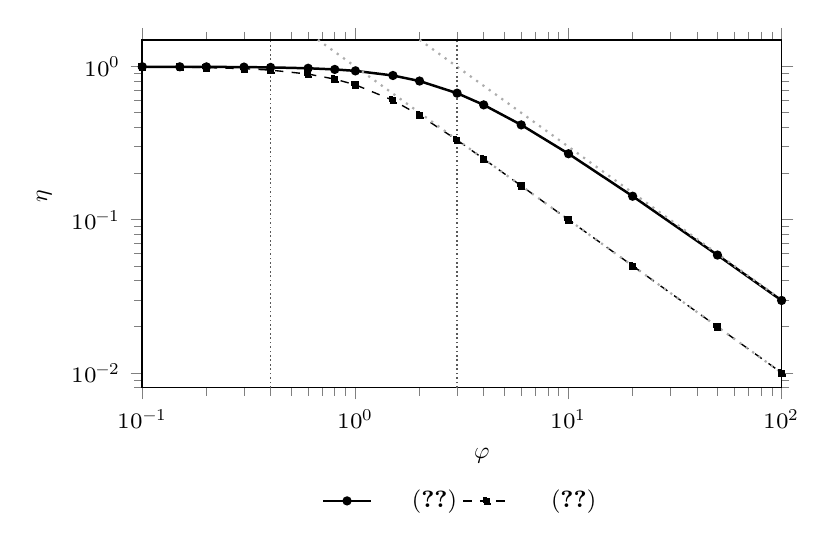
\begin{tikzpicture}
\begin{axis}[
  width=\onecolwidth,
  height=6.0cm,
  xlabel={内扩散模数 $\varphi$},
  ylabel={有效因子 $\eta$},
  xmode=log, ymode=log,
  xmin=0.1, xmax=100, ymin=0.008, ymax=1.5,
  legend style={at={(0.5,-0.26)}, anchor=north, legend columns=2, draw=none, fill=none},
]
\addplot[mainline, mark=*, mark size=1.2pt] coordinates {
  (0.10,0.9993) (0.15,0.9985) (0.20,0.9973) (0.30,0.9941) (0.40,0.9895)
  (0.60,0.9768) (0.80,0.9598) (1.00,0.9391) (1.50,0.8762) (2.00,0.8060)
  (3.00,0.6716) (4.00,0.5630) (6.00,0.4167) (10.00,0.2700) (20.00,0.1425)
  (50.00,0.0588) (100.00,0.0297)};
\addlegendentry{球形，式~\eqref{eq:ch10-eta}}
\addplot[thinline, dashed, mark=square*, mark size=1.2pt] coordinates {
  (0.10,0.9967) (0.15,0.9926) (0.20,0.9869) (0.30,0.9710) (0.40,0.9499)
  (0.60,0.8951) (0.80,0.8300) (1.00,0.7616) (1.50,0.6034) (2.00,0.4820)
  (3.00,0.3317) (4.00,0.2498) (6.00,0.1667) (10.00,0.1000) (20.00,0.0500)
  (50.00,0.0200) (100.00,0.0100)};
\addlegendentry{平板，式~\eqref{eq:ch10-eta}}
\addplot[accentsoft, dotted, thick, forget plot] coordinates {(2,1.5)(100,0.03)};
\addplot[accentsoft, dotted, thick, forget plot] coordinates {(0.667,1.5)(100,0.01)};
\addplot[accent, densely dotted, forget plot] coordinates {(0.4,0.008)(0.4,1.5)};
\addplot[accent, densely dotted, forget plot] coordinates {(3,0.008)(3,1.5)};
\end{axis}
\end{tikzpicture}
\caption{有效因子随 Thiele 模数的变化（一级反应，双对数坐标）。读图看三处：$\varphi<0.4$
时两曲线都在 $0.95$ 以上（内扩散可忽略）；$\varphi>3$ 后两曲线都变成直线且斜率 $-1$，
即 $\eta\approx1/\varphi$（强内扩散）；两条点线是渐近线 $3/\varphi$（球）与 $1/\varphi$
（板），两条竖虚线为 $\varphi=0.4$ 与 $\varphi=3$。条件与局限：等温、一级不可逆反应、
$D_e$ 为常数、球与平板两种理想几何；$\eta$ 由式~\eqref{eq:ch10-eta} 计算，属模型计算。
\modelmark}
\label{fig:ch10b-etaphi}
\end{figure}

\begin{obs}
读图~\ref{fig:ch10b-etaphi}：$\varphi=0.4$ 处球形 $\eta=0.990$、平板 $\eta=0.950$；
$\varphi=1$ 处两者分别为 $0.939$ 与 $0.762$；$\varphi=10$ 处分别为 $0.270$ 与 $0.100$，
而渐近线 $3/\varphi$ 与 $1/\varphi$ 在同一点给出 $0.300$ 与 $0.100$。$\varphi$ 从 $0.4$
增到 $10$（$25$ 倍），球形 $\eta$ 从 $0.99$ 掉到 $0.27$（$3.7$ 倍）。
\end{obs}

\begin{infer}
（1）$\varphi$ 的 $25$ 倍变化只换来速率 $3.7$ 倍的下降——因为强扩散区里
$\eta\propto1/\varphi$，而 $\varphi\propto R$，所以\textbf{速率大致与粒径成反比}：
粒径减半，总包速率约翻倍，而\textbf{本征速率常数一点没变}。这正是「改变粒径看转化率」
能判别内扩散的原因。（2）平板与球的曲线在两端靠近、在中间分开，说明\textbf{几何形状
只影响系数，不影响标度}；因此工程上常用一个统一长度把不同形状折到同一条曲线上。
（3）$\varphi>3$ 后两条曲线平行（斜率同为 $-1$），故\textbf{强内扩散下表观活化能减半}
——这是内扩散最隐蔽的后果：速率数据看起来仍然「服从 Arrhenius 定律」，只是斜率错了。
\end{infer}

\textbf{表观级数与表观活化能会被改成什么。}对 $m$ 级反应，$r=\eta k_SS_vc_S^m$，
两端取对数后对 $\ln c_S$ 求导得表观级数 $m'=\dd\ln\eta/\dd\ln c_S+m$，即 $m'$ 由
$\eta$ 与 $c_S$ 的关系决定。把 $\varphi$ 写成浓度的函数
$\varphi_S=R\sqrt{S_vk_Sc_S^{m-1}/D_e}$（平板同理）再代入 $\eta\approx1/\varphi$，
可得\src{S2 §10.4.2，书内 p.774—775 / PDF p.263—264}：

\begin{itemize}
\item \textbf{分子扩散}：$D_{ej}$ 与总压成反比（$D_e\propto1/p\propto1/c_S$），
故 $m'=m/2$；
\item \textbf{Knudsen 扩散}：$D_{Ke}$ 与压力无关，故 $m'=(m+1)/2$。
\end{itemize}

\textbf{表观活化能}：定义 $E_a=-R\,\dd(\ln\eta k_S)/\dd(1/T)$，本征值
$E=-R\,\dd(\ln k_S)/\dd(1/T)$，则 $E_a/E$ 是 $\eta$ 的函数；在强内扩散区
（$\varphi>3$、$\eta\approx1/\varphi$）有 $E_a/E\approx1/2$
\src{S2 §10.4.2，书内 p.775 / PDF p.264}。注意这两个结论的\textbf{成立前提}：
$m'$ 的两种结果分别假定了分子扩散与 Knudsen 扩散的\textbf{压力依赖}（并默认理想气体
$c\propto p$，过渡区两者叠加时两个公式都不适用）；$E_a\approx E/2$ 假定了
$D_e$ 与温度无关。\textbf{若把扩散系数的温度依赖算进去，强内扩散的表观活化能应写成
$E_a\approx(E+E_D)/2$}（$E_D$ 为扩散活化能，分子扩散约 $1.5RT$、Knudsen 扩散约
$0.5RT$）——本项为学科标准结果，原书未展开，列此以免把 $E/2$ 当成严格值。

\textbf{不同几何的互检（一个可验算的旁证）。}为使各几何模型可比，引入长度参数
$d=$颗粒体积$/$扩散面积\src{S2 §10.4.3，书内 p.776 / PDF p.265}：平板 $d=L$，
圆球 $d=R/3$（因 $V_p/S_{\text{外}}=R/3$）。于是用统一长度表达的模数为
$\varphi_S/3$——\tocheck{未对照原页面图像：原书此处 OCR 作「以统一长度表达的
$\varphi=\tfrac12\varphi_S$」。按 $\varphi_S=3\varphi_{\text{统一}}$（即 $\varphi_S/3$）
计算：统一模数为 $1$ 时 $\eta_{\text{板}}=0.762$、$\eta_{\text{球}}(\varphi_S=3)=0.672$，
差 $0.090$，恰与原书「对一级反应 $\eta_L$ 最大而 $\eta_S$ 最小，两者相差约 $0.09$」
相符（差值在统一模数 $1.15$ 附近达到极大 $0.092$）；若按 $\tfrac12$ 折算则得 $0.32$，
明显不符。故疑 OCR 的「$1/2$」应为「$1/3$」，引用前请核对页面。}

\subsubsection{复杂情形：双组分、摩尔数变化、双曲线速率方程、可逆反应}

实际体系很少满足上一小节的四条假定，原书逐项讨论了偏离的后果
\src{S2 §10.4.3，书内 p.776—777 / PDF p.265—266}。

\textbf{（1）双组分反应。}反应对两个物种都是一级、其中一个（如 $\mathrm{B_1}$）受内扩散
控制时，以平板模型为例，其内扩散模数为

\begin{equation}
\varphi_{L,1}=L\sqrt{\frac{k_SS_vc_2}{(D_e)_1}}
\label{eq:ch10-bicomp}
\end{equation}

当 $\eta$ 小于 $0.4$ 时它可近似为 $1/\varphi_{L,1}$，此时\textbf{表观级数对 $\mathrm{B_1}$
仍是一级，对 $\mathrm{B_2}$ 却变成 $3/2$ 级}（指 Knudsen 扩散区）。
\tocheck{未对照原页面图像：式 (10-122) 的分子（$c_2$ 是否带幂次、下标 $(D_e)_1$ 的位置）
与「$\eta$ 小于 $0.4$」这一临界表述均按 OCR 转写，数值边界请核页面。}

\textbf{（2）反应伴有摩尔数变化。}在分子扩散或过渡区中，反应总摩尔数增加使反应物更难
扩散进入颗粒，$\eta$ 更低；总摩尔数减少则相反。定量说明需引入摩尔数增加 $\delta$ 与
摩尔分数 $Y_1$ 的乘积作参数：对圆球状催化剂，若 $\varphi_S<3$ 而主要反应物
$\mathrm{B_1}$ 的 $\delta Y_1$ 在 $\pm0.5$ 以内，$\eta$ 的变化不超过 $10\%$。

\textbf{（3）颗粒形状。}除球与板之外还有圆柱、长杆模型。$\eta$—$\varphi$ 曲线对不同
几何并不相同：$\varphi$ 很小或很大时各形状差别相当小，在统一模数 $1$ 附近差别最大
（数值互检见上一小节）；圆柱模型居中。

\textbf{（4）双曲线式速率方程的有效因子。}用 L-H 表达式时 $\eta$ 与 $\varphi$ 的关系
复杂得多，需引入两个组合参数 $K_d$ 与 $v_d$\src{S2 §10.4.3，书内 p.776—777 /
PDF p.265—266}：

\begin{equation}
K_d=\frac{K_1-D_1\sum_i\nu_iK_i/D_i}
{1+\sum_iK_i\bigl(p_i+\nu_ip_1D_1/D_i\bigr)},\qquad
v_d=\frac{D_2p_2}{\nu_2D_1p_1}-1
\label{eq:ch10-kd}
\end{equation}

式中 $K_1$、$D_1$、$p_1$ 是双组分中主要反应物的吸附平衡常数、扩散系数与分压，带下标
$i$ 的是其他组分。选择反应物时要使 $v_d\ge0$。若各 $K_1$ 都很小，$K_d\to0$，反应
趋于一级；对零级反应 $K_dp_1\to\infty$，对高级次反应 $K_dp_1$ 为负；
$K_dp_1$ 最小为 $-1$，对应强产物阻抑。$p_2$ 或 $D_2$ 远大于 $\mathrm{B_1}$ 的相应值时
$v_d$ 较大。原书的 $\eta$—$\varphi_L$ 曲线族（图 10-6）给出三条要点
\src{S2 §10.4.3，书内 p.777 / PDF p.266}：$K_dp_1$ 或 $v_d$ 越大曲线位置越高；
在 $K_dp_1$ 很小时 $v_d$ 的影响很小；\textbf{当 $v_d>0.1$ 且 $K_dp_1\ge10$ 时，
$\eta$ 在某些 $\varphi_L$ 区间内可以比 $1$ 大很多}，而且部分曲线中段的点线连接处
实际是 $\eta$ 多值区间，对应非稳态操作。这两点与\textbf{非恒温}扩散控制的速率行为
相似，读图时不要把它们混为一谈。
\tocheck{未对照原页面图像：式 (10-123) 的完整形式（$K_d$ 分子的符号、$v_d$ 的定义与
$K_dp_1$ 的取值范围）在 OCR 中严重失真，此处按可见结构转写，引用前须核对页面。}

\textbf{（5）可逆反应。}存在显著逆向反应时 $\eta$ 的解析更复杂，一般要在同样的
$\varphi_L$ 下得到\textbf{更低}的 $\eta$。原书给出的一组对比：对一级不可逆反应，
$\varphi_L=0.55$ 及 $3.15$ 时 $\eta$ 约为 $1.0$ 与 $0.30$；若为一级可逆反应、
平衡转化率 $50\%$，同样 $\varphi_L$ 下 $\eta$ 降为 $0.80$ 与 $0.16$。对高级数反应
影响更大。\src{S2 §10.4.3，书内 p.777 / PDF p.266}
\textbf{实用含义}：在接近平衡的条件下用恒温不可逆模型的 $\eta$ 去校正速率，会\textbf{高估}
有效因子，从而低估内扩散的严重程度。

\subsubsection{非恒温粒内传质：非恒温有效因子}

催化剂本身导热率低、扩散系数大、反应热效应大时，颗粒内温度会显著不同于外表面温度。
有效因子仍定义为实测速率与「无粒内传热传质限制」速率的比值，但解热量与物料衡算的
联立方程时须引入两个无因次参数\src{S2 §10.4.4，书内 p.778 / PDF p.267}：

\begin{equation}
\gamma=\frac{E}{RT},\qquad
\beta=\frac{c_s(-\Delta H)D_e}{\lambda_pT_s}
\label{eq:ch10-gammabeta}
\end{equation}

式中 $\Delta H$ 为反应焓变，$\lambda_p$ 为多孔颗粒的热导率。对放热反应 $\beta>0$，其
物理意义是\textbf{稳态下颗粒内可能的最大温差与外表面温度之比}
$(T-T_s)_{\max}/T_s$。原书给出的典型值：$\gamma=20$ 对应 $E\approx100$\,\unit{kJ.mol^{-1}}、
$T\approx600$\,\unit{K}（按 $\gamma=E/RT$ 核算为 $99.8$\,\unit{kJ.mol^{-1}}，自洽），
$\beta$ 在 $\pm0.8$ 之间作出一族 $\eta$—$\varphi_S$ 曲线，$\beta=0$ 即恒温情况。
\src{S2 §10.4.4，书内 p.778 / PDF p.267}

原书对图 10-7 的读法有三条结论，都是恒温模型给不出的
\src{S2 §10.4.4，书内 p.779 / PDF p.268}：（1）$\varphi_S$ 高时各曲线的 $\eta$ 仍与
$\varphi_S$ 成反比，与恒温情况相同；（2）$\beta>0$ 时，\textbf{对一定的 $\varphi_S$，
$\eta$ 可以超过、甚至远超过 $1$}——因为颗粒内温升引起的速率增加远超过浓度降低引起的
速率下降；（3）$\varphi_S$ 较小的区间里 $\eta$ 是\textbf{多值}的，同一个 $\varphi_S$
下可以有三个 $\eta$ 值而放热与散热都能平衡，其中间值对应\textbf{亚稳态}：稍有扰动即
破坏，颗粒温度不是升到与较高 $\eta$ 相应的稳态（控速步骤为气固传质），就是降到与较低
$\eta$ 相应的稳态（表面化学反应控速）。

\begin{pitfall}
\textbf{非恒温体系的两个反直觉之处。}（1）看到 $\eta>1$ 不要先怀疑算错——在放热反应
且粒内温差显著时它是物理上可能的；反过来，\textbf{若用恒温模型解释 $\eta>1$，会把
「本征速率被低温区低估」误读成「模型形式错误」。}（2）$\eta$ 多值意味着\textbf{同一套
操作条件可能出现两个稳定态}，实验上表现为升温和降温测得的速率不重合（滞后）。此时
不能用单值 $\eta$ 曲线做数据校正，必须先判定处在哪个态。
\end{pitfall}

\subsubsection{判据：假设、失效条件与可操作的实验}

判据的作用是把「传递有没有干扰」变成一个\textbf{可算的数}，并用三组实验去检验它。
\textbf{三个判据的前提是同一条}：式~\eqref{eq:ch10-basis} 的速率基准必须统一。

\begin{principle}
\textbf{三个判据（全部写成体积基准；质量基准为等价写法）。}
\textbf{（1）外扩散：Damk\"ohler 数判据}\src{S2 §10.5.4，书内 p.791—792 /
PDF p.280—281}，对 $m$ 级反应
\begin{equation}
Da=\frac{r_vR}{k_mc_B}<\frac{0.15}{m},
\qquad\text{质量基准：}\ Da=\frac{\rho_pr_mR}{k_mc_B}
\label{eq:ch10-da}
\end{equation}
式中 $c_B$ 为组分 $\mathrm{B_1}$ 在流体相的浓度，$R$ 为颗粒半径，$k_m$ 为颗粒外膜的
传质系数。\textbf{量纲}：
$\unit{mol.m^{-3}.s^{-1}}\times\unit{m}\big/\bigl(\unit{m.s^{-1}}\times
\unit{mol.m^{-3}}\bigr)$——无量纲；质量基准式中的
$\unit{kg.m^{-3}}\times\unit{mol.kg^{-1}.s^{-1}}$ 恰好还原为
$\unit{mol.m^{-3}.s^{-1}}$，故两式\textbf{数值恒等}。

\textbf{（2）内扩散：Weisz--Prater 判据}\src{S2 §10.5.4，书内 p.792 / PDF p.281}。
它可以直接由有效因子的定义推出，不必知道本征动力学：把观测速率
$r_v=\eta k_vc_S$ 代入 $\eta\varphi^2$ 得
\begin{equation}
\Phi\equiv\eta\varphi^{2}=\frac{r_vR^{2}}{D_ec_B},
\qquad\text{质量基准：}\ \Phi=\frac{\rho_pr_mR^{2}}{D_ec_B}
\label{eq:ch10-wp}
\end{equation}
式中 $D_e$ 为有效扩散系数。\textbf{量纲}：
$\unit{mol.m^{-3}.s^{-1}}\times\unit{m^2}\big/\bigl(\unit{m^2.s^{-1}}\times
\unit{mol.m^{-3}}\bigr)$——无量纲。由于 $\Phi=\eta\varphi^{2}$ 把两个未知量绑在一起，
判据本身只给 $\Phi$，\textbf{阈值必须按「容许多大的 $\eta$ 下降」来定}。对等温球形
颗粒、一级反应，把式~\eqref{eq:ch10-eta} 的 $\eta(\varphi)$ 逐点代入可算得：
$\Phi=0.3$ 对应 $\varphi\approx0.55$、$\eta\approx0.98$；$\Phi=1$ 对应
$\varphi\approx1.03$、$\eta\approx0.94$。因此原书「一级反应 $\Phi<1$ 可保证有效因子
\textbf{小于} $0.95$」的方向应为\textbf{大于}——$\Phi<1$ 保证的是 $\eta>0.94$；
若要求 $\eta>0.95$ 需 $\Phi<0.74$，要求 $\eta>0.99$（即常用界 $\varphi<0.4$）则需
$\Phi<0.16$。平板几何在同一个 $\Phi$ 下 $\eta$ 更低（$\Phi=1$ 时 $\eta\approx0.70$），
所以\textbf{报阈值必须连几何与级数一起报出}；下文按惯例写「一级 $\Phi<1$、二级
$\Phi<0.3$」，其中 $\Phi<1$ 是\textbf{不出现严重内扩散}的设计上限，不等于
「$\eta$ 仍在 $0.95$ 以上」。
\textbf{注意}：质量基准式里的 $\rho_p$ 就是\textbf{把质量速率换算成体积速率的那一个
因子}，它只出现一次。

\textbf{（3）相间传热：Mears 判据}（$\eta>0.95$ 的条件）
\src{S2 §10.5.4，书内 p.791—792 / PDF p.280—281}：
\begin{equation}
\frac{r_v(-\Delta H_r)R}{h_BT_B}<0.15\,\frac{\mathscr{R}T_B}{E}
\label{eq:ch10-mears}
\end{equation}
式中 $h_B$ 为相间传热系数，$T_B$ 为流体温度，$E$ 为活化能；为免同一字母歧义，
\textbf{右侧的气体常量记作 $\mathscr{R}$}，左侧的 $R$ 仍是颗粒半径。
\textbf{量纲}：左侧
$\unit{mol.m^{-3}.s^{-1}}\times\unit{J.mol^{-1}}\times\unit{m}\big/
\bigl(\unit{W.m^{-2}.K^{-1}}\times\unit{K}\bigr)
=\unit{J.m^{-2}.s^{-1}}\big/\unit{W.m^{-2}}$——无量纲（$\unit{W}=\unit{J.s^{-1}}$）；
右侧 $\unit{J.mol^{-1}.K^{-1}}\times\unit{K}\big/\unit{J.mol^{-1}}$——无量纲。
质量基准式左分子写成 $\rho_pr_m(-\Delta H_r)R$，同样数值恒等。
颗粒半径与几何的关系：由 $S_{\text{外}}/V_p=3/R$ 得 $R=3V_p/S_{\text{外}}$，
非球形颗粒按此折等效半径，不要直接拿筛分粒度。
\end{principle}

\begin{figure}[htbp]
\centering
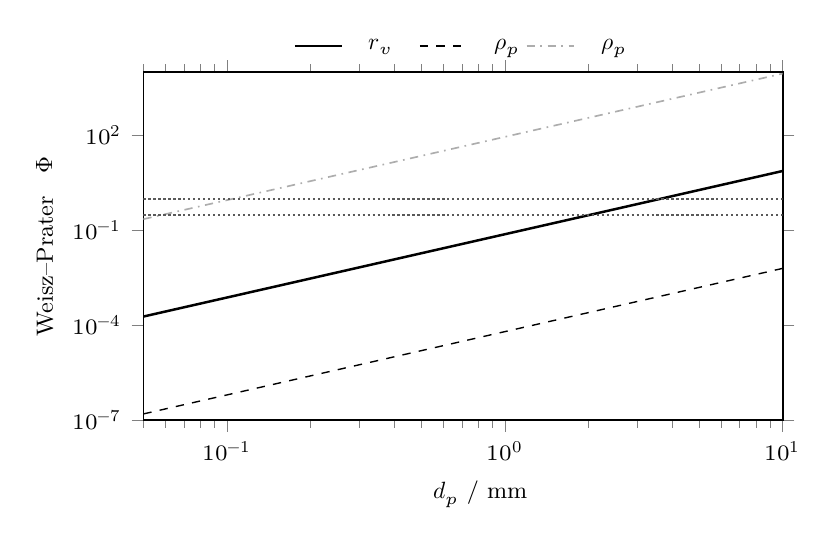
\begin{tikzpicture}
\begin{axis}[
  width=\onecolwidth,
  height=6.0cm,
  xlabel={颗粒直径 $d_p$ / \unit{mm}},
  ylabel={Weisz--Prater 数 $\Phi$},
  xmode=log, ymode=log,
  xmin=0.05, xmax=10, ymin=1e-7, ymax=1e4,
  legend style={at={(0.5,1.02)}, anchor=south, legend columns=3, draw=none, fill=none},
]
\addplot[mainline, domain=0.05:10, samples=60]{0.075*x^2};
\addlegendentry{正确：$r_v$ 基准}
\addplot[thinline, dashed, domain=0.05:10, samples=60]{6.25e-5*x^2};
\addlegendentry{少乘 $\rho_p$}
\addplot[accentsoft, dashdotted, domain=0.05:10, samples=60]{90*x^2};
\addlegendentry{多乘 $\rho_p$}
\addplot[accent, densely dotted, thick, forget plot] coordinates {(0.05,1)(10,1)};
\addplot[accent, densely dotted, thick, forget plot] coordinates {(0.05,0.3)(10,0.3)};
\end{axis}
\end{tikzpicture}
\caption{同一条 Weisz--Prater 判据、同一个观测速率，三种速率基准下 $\Phi$ 随粒径的变化
（双对数，$\Phi\propto d_p^{2}$）。读图看三线的相对位置：正确基准居中；「少乘 $\rho_p$」
那条线偏低 $1/1200$（判据失效），「多乘 $\rho_p$」那条线偏高 $1199$ 倍（误判），两条
错误线彼此相距 $1.44\times10^{6}$ 倍；两条水平点线为阈值 $\Phi=1$（设计上限）与
$\Phi=0.3$（二级反应用；对一级反应它给出 $\eta>0.95$）。
条件与局限：等温球形颗粒、一级反应，取
$r_m=9$\,\unit{mmol.g^{-1}.h^{-1}}、$\rho_p=1200$\,\unit{kg.m^{-3}}、
$D_e=1.0\times10^{-6}$\,\unit{m^2.s^{-1}}、$c_B=10$\,\unit{mol.m^{-3}}
（教学设定数值），曲线为模型计算。\modelmark}
\label{fig:ch10-wp}
\end{figure}

\begin{obs}
读图~\ref{fig:ch10-wp}：正确基准下 $\Phi=0.075\,d_p^{2}$，与 $\Phi=0.3$ 相交于
$d_p=2.0$\,\unit{mm}，与 $\Phi=1$ 相交于 $d_p=3.65$\,\unit{mm}；「多乘 $\rho_p$」那条线
是 $90\,d_p^{2}$，与 $\Phi=1$ 相交于 $d_p=0.105$\,\unit{mm}；「少乘 $\rho_p$」那条线是
$6.25\times10^{-5}d_p^{2}$，在横轴到 $10$\,\unit{mm} 时 $\Phi$ 仅 $6.3\times10^{-3}$，
始终没有触及任何阈值。三条线在任意横坐标上的比值恒为 $1/1200$（少乘线/正确线）与
$1200$（多乘线/正确线）。三条线的系数可以把量纲检查直接算出来：$r_v=\rho_pr_m
=1200\times2.5\times10^{-3}=3.0$\,\unit{mol.m^{-3}.s^{-1}}，
$\Phi=r_vR^{2}/(D_ec_B)$ 中 $R=d_p/2$，故
$\Phi=r_vd_p^{2}/(4D_ec_B)=3d_p^{2}/(4\times10^{-5})=0.075\,d_p^{2}$
（$d_p$ 以 \unit{mm} 计）；少乘线用 $r_m$ 代替 $r_v$，系数即
$2.5\times10^{-3}/(4\times10^{-5})=6.25\times10^{-5}$；多乘线用 $r_v\rho_p$，
系数即 $0.075\times1200=90$。
\end{obs}

\begin{infer}
（1）三条线来自\textbf{同一组速率数据}，差别只有一个颗粒密度 $\rho_p$；结论却完全相反：
正确基准说「粒径超过约 $2$\,\unit{mm} 就要担心内扩散」，多乘 $\rho_p$ 说「$0.1$\,\unit{mm}
以上都不合格」（会把合格数据误判成受内扩散控制而白白丢弃），少乘 $\rho_p$ 说
「$10$\,\unit{mm} 也通过」（判据失去意义，把扩散控制当本征动力学）。（2）因此
\textbf{判据的第一步不是代入数字，而是写出基准}；判据不自检量纲就等于没做。
（3）判据的数量级特征是 $\Phi\propto d_p^2$：粒径减半，$\Phi$ 降到 $1/4$——这就是
「改变粒径看转化率」这组实验之所以有效的根据。
\end{infer}

\begin{measure}
\textbf{把判据做成实验：三组自变量、三条判读规则。}
\src{S2 §10.5.4，书内 p.791—792 / PDF p.280—281}
\textbf{实验一（外扩散）——同一接触时间下改变线速。}在同一反应器内随质量流速改变而
相应增减催化剂用量，使接触时间 $W/F$ 不变；若质量流速增大而转化率趋于稳定值，
外扩散已消除。也可用截面积相同的两个反应器装不同量催化剂、按比例引入流量：高流速区
两者转化率无差别，低流速区不同。还可在同一反应器中改变流量、在不同温度下求表观速率
常数：不同流量的曲线重合则无外扩散，高温下不重合则外扩散在起作用。\textbf{判读}：
取「流速高到对转化率无明显影响」的区间做动力学实验，再用
式~\eqref{eq:ch10-da} 复核。
\textbf{实验二（内扩散）——同一空速下改变粒径。}从同一批催化剂取不同粒径的几份样品，
测同一空速下的转化率；粒径减小时转化率上升到一极限值，取与该极限值相应的粒径
\textbf{以下}的催化剂作研究，内扩散即可排除。\textbf{判读}：用
式~\eqref{eq:ch10-wp} 复核，且 $\Phi$ 必须随 $d_p^2$ 变化，若实测 $\Phi$ 与粒径无关，
说明 $r_v$、$D_e$ 或 $c_B$ 的取法有问题。
\textbf{实验三（温度）——把三个区画出来。}前两组实验必须在\textbf{整个实验温度区间}
都通过；只在高温区通过、低温区未检验的数据不可外推。\textbf{还要满足理想活塞流的
三个几何条件}：反应管内径至少为颗粒直径的 $10$ 倍以上；气-固反应床层长度至少为粒径的
$50$ 倍以上；液-固反应床层长度至少为粒径的几百倍以上（否则沟流或轴向弥散破坏活塞流
假定）。
\end{measure}

\begin{table}[htbp]
\centering
\caption{三个判据的假设与失效条件。左列三式均用体积基准 $r_v$；换成质量基准时
\textbf{每式恰好乘一个} $\rho_p$——不是每式各自再补一个。
\src{据 S2 §10.5.4，书内 p.790—793 / PDF p.279—282 归纳。}}
\label{tab:ch10-criteria}
\begin{tabularx}{\textwidth}{@{}l X X@{}}
\toprule
判据 & 表达式（体积基准） & 主要假设与失效条件 \\
\midrule
Damk\"ohler 数（外扩散） & $Da=r_vR/(k_mc_B)<0.15/m$ &
假设等温、稳态、外膜传质为串联阻力、对 $\mathrm{B_1}$ 为 $m$ 级。
\textbf{失效}：$m\le0$ 时阈值发散（零级反应不适用）；强放热时必须同时用 Mears 判据；
$k_m$ 须由 $Re$、$Sc$ 在关联式适用范围内取得；非球形颗粒的 $R$ 要按 $3V_p/S_{\text{外}}$
折算 \\
Weisz--Prater 数（内扩散） & $\Phi=r_vR^{2}/(D_ec_B)$，一级 $<1$、二级 $<0.3$ &
假设等温、$D_e$ 为常数、单一反应、几何为球或板、级数已知。
\textbf{失效}：非等温（$\beta$ 不可忽略时 $\eta$ 可大于 $1$，恒温判据给出的「安全」
结论不可靠）；过渡区 $D_e$ 随组成变化；可逆反应与强产物阻抑（同一 $\varphi$ 下 $\eta$
更低甚至多值）；只能判「是否受限制」，不能给出本征参数 \\
Mears 判据（相间传热） & $r_v(-\Delta H_r)R/(h_BT_B)<0.15\mathscr{R}T_B/E$ &
假设稳态、相间膜传热、目标为 $\eta>0.95$、活化能 $E$ 已知、温度用绝对温标。
\textbf{失效}：$E$ 未知时右侧无法计算（用表观 $E$ 会引入偏差）；粒内温差显著时须改用
非恒温有效因子（式~\eqref{eq:ch10-gammabeta} 的 $\beta$）判断，Mears 判据管不到粒内 \\
\bottomrule
\end{tabularx}
\end{table}

\begin{dataflow}
\textbf{一次完整的传递影响判定（判据 + 实验互为回查）。}
（1）写出速率基准：把分析数据换成 $r_m$，再由式~\eqref{eq:ch10-basis} 得 $r_v$；
（2）取几何参数：$R=3V_p/S_{\text{外}}$、$\rho_p$、$c_B$ 与温度；
（3）算 $D_e$：按表~\ref{tab:ch10-diffmech} 判断机制（孔径与平均自由程比较），
分子与 Knudsen 并存时用 $1/D_e=1/D_{Ke}+1/D_{ej}$；
（4）按表~\ref{tab:ch10-criteria} 逐项算 $Da$、$\Phi$，并算热判据；
（5）用实验一、二、三检验判据的结论：判据说「通过」而实验显示转化率随线速或粒径变化，
则优先相信实验——通常是 $D_e$ 取错（无反应下测的值与反应下可差 $4$—$5$ 倍）
或 $k_m$ 的关联式超出适用范围；
（6）判据通过后，才可以在本征动力学区拟合参数，并在论文里同时报出判据的数值与基准。
\end{dataflow}

\begin{pitfall}
\textbf{本节的五个误判，前三个直接毁掉结论。}
（1）\textbf{把扩散控制当本征动力学}：$\varphi>3$ 时速率与粒径成反比、表观活化能减半、
级数被改写（分子扩散 $m/2$、Knudsen $(m+1)/2$），此时得到的「动力学参数」是设备参数
的函数，外推到工业粒度必然出错。识别特征是\textbf{改变线速或粒径时转化率变}。
（2）\textbf{速率基准混用}：把 $\unit{mol.g^{-1}.s^{-1}}$ 的数值直接代入
式~\eqref{eq:ch10-da} 或式~\eqref{eq:ch10-mears}，得到的量单位是
$\unit{m^3.kg^{-1}}$——\textbf{有量纲，无论数值大小都不成判据}；这是「看起来通过判据」
的假阴性来源。\textbf{自检只能靠逐式展开 SI 单位}。
（3）\textbf{重复计入密度}：式~\eqref{eq:ch10-wp} 用 $r_v$ 时不再乘 $\rho_p$，
用 $r_m$ 时乘\textbf{一次} $\rho_p$；写成 $r_v\rho_pR^2/(D_ec_B)$ 等于多算一个
$\rho_p$（图~\ref{fig:ch10-wp} 中就是偏上 $1200$ 倍那条线），而漏乘则偏下 $1200$ 倍。
（4）\textbf{忽略热点与温度梯度}：$\eta>1$、同一操作点两个稳定态、升降温数据不重合，
都可能是非恒温的表现，而不是「模型错了」；强放热反应里相间温差可远大于粒内温差。
（5）\textbf{用 $R^2$ 判定模型优劣}：判据与模型检验的判据是残差结构与参数稳定性，
$R^2$ 高只说明曲线穿过了数据点。
\end{pitfall}

\begin{crosscheck}
\textbf{判据之间、判据与实验之间的回查关系。}
（1）\textbf{顺序}：外扩散与内扩散是串连的（外扩散在前），必须先排外扩散再排内扩散；
若 $Da$ 不通过，$\Phi$ 里用的 $r_v$ 本身就含外扩散的影响，判据失去意义。
（2）\textbf{两类判据互补}：$Da$ 与 $\Phi$ 管等温情形，Mears 判据管相间传热，粒内温差
由 Prater 数 $\beta$（式~\eqref{eq:ch10-gammabeta}）管——三者的检查对象不同，
不能用一个代替另一个。
（3）\textbf{与 $D_e$ 的测量方式回查}：无反应下估算或测定的扩散系数与反应条件下的
实际有效扩散系数\textbf{可差 $4$—$5$ 倍}（反应与非反应时扩散通量比相差甚大，且与表面
扩散、孔径分布不均有关），因此求内扩散参数时优先用\textbf{反应条件下}的数据
（改变粒径求有效因子、单锭扩散反应器等），具体方法见本章后半部分。
（4）\textbf{与独立实验回查}：判据说「本征区」而瞬态或同位素实验给出的吸附量与由稳态
数据反推的 $K$ 矛盾时，问题通常不在判据，而在数据窗口没有覆盖机理发生变化的区间。
\end{crosscheck}
}{}
\IfFileExists{chapters/parts/ch10-c.tex}{% ================================================================
%  chapters/parts/ch10-c.tex
%  第 10 章  多相催化反应动力学（分片 c）
%  源：S2（下册）第 10 章，书内 p.779—806 / PDF p.268—295
%  覆盖：10.5 动力学测定方法和实验装置；10.6 非稳态催化过程动力学；10.7 结论
%  说明：本分片负责 10.5 与 10.6（分片 b 负责 10.3 与 10.4）。
%        10.5.1—10.5.4 的源文本区间为书内 p.779—792 / PDF p.268—281。
% ================================================================

\subsection{动力学测定方法和实验装置}
\label{sec:ch10-measure}

在一般多相催化反应器上得到的实验结果里，化学反应与传递过程总是不同程度地耦合在一起。
用这种耦合数据，无论设计反应器还是改进催化剂，都是困难的。因此必须先靠适当的实验工具
和条件把两者分离开，才谈得上求取\textbf{本征动力学参数}（速率常数、活化能、反应级数、
吸附平衡常数）与\textbf{传递过程参数}（有效扩散系数、传质与传热系数）。分离的手段有两类：
选对反应器与操作区，以及用非稳态实验给稳态实验补上它拿不到的信息。
\src{S2 §10.5 引言，书内 p.779 / PDF p.268}

\begin{probout}
本章的前半部分交付速率方程，而速率方程能否被信任，取决于数据是在哪个\textbf{动力学区}
测出来的。本分片回答四个问题：（1）实验室反应器种类繁多，凭什么从中选一个——
它能测什么、不能测什么；（2）「已排除外扩散」「已排除内扩散」不是一句声明，而是
可以执行的\textbf{三组实验}与三个\textbf{定量判据}，它们具体怎么做、阈值是多少；
（3）稳态动力学给出的是速率对流体相组成的依赖，它\textbf{给不出吸附态的浓度与寿命}，
这个缺口由哪些非稳态方法补、各自的时间尺度是多少；（4）催化剂活性随时间变化、
多稳态与振荡这些「非稳态」现象，如何做动力学处理。
\end{probout}

\subsubsection{实验室反应器的选型逻辑}

反应器种类繁多，\textbf{但并不是都可以用来求取动力学参数}。选型依据是催化反应的特点
和所要获取的信息，其中有三个条件优先于其他一切考虑\src{S2 §10.5.1，书内 p.779 /
PDF p.268}：

\begin{keycond}
（1）\textbf{恒温性}——温度对反应速率的影响是指数性的，反应器内任何温度梯度都会直接
变成速率误差；对复杂反应，温度偏差还会改变选择性。（2）\textbf{停留（接触）时间的确切性
或均一性}——数据要与模型比较，就必须知道每个流体元在催化剂上待了多久。（3）\textbf{产物
取样和分析是否容易}——分析精度往往才是真正的限制环节。至于反应器制作是否价廉简易，
\textbf{应服从实验需要}，不能作为选型的首要依据。
\end{keycond}

\textbf{（1）积分反应器。}管式反应器中装填足量催化剂以达到较大转化率，进出口组成差别
显著，无法用某个平均值代表全反应器的组成。因此积分反应器只能给出\textbf{转化率（或
生成率）对空时的积分数据}，但在分析技术和方法上要求不高。它在动力学研究中又分两种。
\textbf{恒温积分反应器}简单价廉，只要可能总应首先考虑；其困难在于转化率高、反应热稍大
就难以恒温。常用对策有三条：\textbf{减小管径}（使径向温度均匀，管径为催化剂粒径 4 倍
以上时减小管径对恒温性的改善仍很明显，但管径过小会加剧沟流引起的壁效应，使转化率
偏低）、\textbf{用恒温导热介质}（熔融金属、熔盐、流沙浴；流沙浴可达 $1000$\,\degC，
控温快而简易，即使放热量较大的氧化反应也可用）、\textbf{用惰性物质稀释催化剂}
（强放热反应用刚玉、石英砂等大热容粒子避免热点）。进一步可采用\textbf{非等比稀释}：
入口处加大稀释比、随转化加深线性降低稀释比，使轴向温度梯度接近于零。
\textbf{绝热积分反应器}为直径均一、装填均匀、绝热良好的圆管；物料预热到一定温度后
通入，沿轴向可测出与反应热量和动力学规律相应的温度分布 $T$–$W$ 曲线。对这条曲线作
解析微分，得到一系列 $\dd T/\dd W$ 与 $\dd^{2}T/\dd W^{2}$；若催化剂有效导热率 $\lambda_e$
已知，且径向梯度与气固间梯度小到可忽略，把这些导数代入反应管的热量衡算（轴向对流项、
有效导热项与反应热源项三项平衡），即可解出不同温度下的 $r_1$；再由能量衡算换算成同一
温度下各组分的摩尔分数 $Y_i$。有了一套不同入口温度下的 $(r_i,\,Y_i)$ 数据，动力学参数
就可以进一步求得——\textbf{但只能用于简单反应}。\src{S2 §10.5.1，书内 p.779—780 /
PDF p.268—269}

\textbf{（2）微分反应器。}若通过床层的转化率很低，进出口组成差别小得足以用平均值代表
全床层组成，却又足够用某种分析方法确定浓度差，则 $\Delta c/\Delta t$ 可近似为
$\dd c/\dd t$ 并等于反应速率 $r$，从而得到与平均组成对应的\textbf{点速率}。单程流通的
管式微分反应器中转化率一般应低于 $5\%$（个别情况允许到 $10\%$）。优点是转化低、发热少、
易恒温、构制简单；但有两个严重问题：一是所得数据常是\textbf{初速}，很难拼出一个合成的
进料来模拟复杂反应在高转化下的组成（补救办法是在微分反应器前串接一个积分转化器，为它
提供所需进料）；二是\textbf{分析精度要求很高}，大多数方法满足不了。\src{S2 §10.5.1，
书内 p.780—781 / PDF p.269—270}

\textbf{（3）循环反应器（无梯度反应器）。}积分反应器分析容易但不能确保理想行为，微分
反应器能确保理想行为但分析困难，\textbf{循环反应器同时具备两者的优点}。反应流体的大部分
用泵在回路中循环，同时连续引入一小股新鲜进料 $F_0$，并从出口放出一股流出物以保持系统
恒压。流体可外循环，也可内循环。设循环量 $F_R$，进料中反应组分 B 的摩尔分数为 $y_0$，
入床层前为 $y_{\mathrm{in}}$，出口为 $y_f$，则按物料衡算

\begin{equation}
x=y_f-y_{\mathrm{in}}=\frac{y_f-y_0}{1+F_R/F_0}
\label{eq:recycle-x}
\end{equation}

当 $F_R\gg F_0$ 时 $y_{\mathrm{in}}\to y_f$、$y_f-y_{\mathrm{in}}\to 0$，反应速率由
微分形式给出

\begin{equation}
r=\frac{\dd x}{\dd W/(F_0+F_R)}\approx\frac{y_f-y_0}{W/F_0}
\label{eq:recycle-r}
\end{equation}

$F_R/F_0$ 一般为 $20$—$40$，远大于 1，相当于把 $y_f-y_{\mathrm{in}}$ 这个微小差值
放大成分析上容易测准的 $y_f-y_0$。由于通过床层的转化率很低，床层温度变化很小；又由于
通过床层的流体量相当大、线速大，\textbf{外扩散影响也可以消除}。代价从分析精度转移到
循环泵：泵不能沾污反应混合物，滞留量要小，循环量要大（$4$~L\,min$^{-1}$ 以上）。
外循环反应器另有两条不足：循环气须冷却到泵体能忍受的温度、出泵后再预热到反应温度；
自由体积与催化剂体积之比高达 $10$—$100$，时间常数很大，从一个操作条件换到另一个
需要较长时间才达稳态，且有利于副反应进行。\textbf{内循环反应器}把循环系统与反应系统
合为一体，自由体积降为催化剂体积的 $3$—$5$ 倍，时间常数显著缩短；装置上部为催化床层
和风道、下部为涡轮叶片，高速转动时强制气流通过催化床再经风道吸回，循环气量可达
$150$~L\,min$^{-1}$，浓度和温度更易达到无梯度状态。它要求轴转速达每分钟数千转，并能
在高温高压下无泄漏、无沾污；目前特殊轴承材料可在 $590$\,\degC 及 $15$~MPa 下操作，
采用磁驱动、全玻璃（或石英）的设计还能避免金属结构材料对催化反应的干扰，且结构简单、
价格低廉。\src{S2 §10.5.1，书内 p.781—782 / PDF p.270—271}

\textbf{（4）搅拌反应器（CSTR）。}当循环比足够高时，循环反应器实际上就是一种全返混
反应器。实验室中与 CSTR 相当的是\textbf{旋转篮式反应器}：催化剂颗粒装在金属网编织的
筐篮中（一般整齐排列），筐篮连于转轴，在反应容器中高速回转，流入的流体在瞬时内与容器
内原有流体完全均匀混合，\textbf{组成与流出物完全相同}。最早的是 Carberry 提出的
notre dame 式；后来的 ICI 式提高了转速、改用磁驱动以防沾污和泄漏并缩小了自由体积；
再后又用加挡板和固定筐篮、使容器高速旋转的办法改进测温和加大流体穿透催化剂的相对速度。
另一种产生气体搅拌效果的办法是让器内气体往复振荡（外部交变电磁场驱动活塞，或由蜂鸣器
带动膜片）。\src{S2 §10.5.1，书内 p.782—783 / PDF p.271—272}

\textbf{（5）流化床反应器与微反应器。}如果催化剂活性在反应过程中逐步上升（诱导期）
或下降（失活），就应改用流化床或微反应器：\textbf{前者适于失活时间以秒计、且有较多
催化剂量可供应用的情况；后者宜于活性变化稍慢而催化剂供应量很少的情况}。流化床反应器
曾用于邻二甲苯氧化动力学研究（内径 $17$~mm、高 $8.2$~m 的不锈钢竖管，含 SO$_2$ 的空气
带入细粒氧化钒催化剂，达稳定两相流动后通入定量邻二甲苯，几分钟即达定态，从上、中、下
三个取样点经烧结不锈钢过滤器滤去催化剂后取样分析）。\src{S2 §10.5.1，书内 p.783 /
PDF p.272}

\textbf{（6）无梯度性能的比较与检验。}动力学反应器基本上就是指无梯度反应器（循环式与
搅拌式）。涡轮或筐篮的转速（或循环量）对无梯度状况有显著影响，后者必须用两类实验检验：
\textbf{用传质实验检验外扩散阻力}（把一定尺寸的萘锭与催化剂装在一起，在 $30$\,\degC 下
测定氮气流中的萘浓度，求出传质因子 $j_D$），以及\textbf{用返混实验表征混合均匀度}
（在进器气流中注入示踪气脉冲，测出器气流中示踪物浓度随时间的变化）。无梯度反应器的
性能比较见表~\ref{tab:ch10-reactor}。\src{S2 §10.5.1，书内 p.783—784 / PDF p.272—273}

选型不是「哪个更好」，而是\textbf{先按所需信息过滤，再按恒温性、接触时间均一性、
分析难度排序}：要宽转化率范围的积分数据选积分床；要点速率选微分床或无梯度反应器；
体系活性快变选流化床或脉冲微反；体系只允许很少催化剂时选微反。表~\ref{tab:ch10-reactor}
把这一逻辑与「能测／不能测」并列，是本节选型的总表。

\begin{table}[tbp]
\centering
\caption{实验室动力学反应器的选型对照。先看第三列\textbf{不能测什么}——反应器的用途
边界比它的优点更需要提前确认；第四列给出该类型成立所必需的约束与本书给出的经验数值。
「流化床」一栏兼收本书讨论的气固流化床，液固浆态体系据本书给出的液固床层条件与
常规实践补充（见本节末注）。\src{据 S2 §10.5.1 与表 10-3，书内 p.779—784 / PDF
p.268—273 整理。}}
\label{tab:ch10-reactor}
{\srcsize
\begin{tabularx}{\twocolwidth}{@{}p{17mm}p{40mm}p{40mm}X@{}}
\toprule
反应器 & 能测什么 & 不能测什么 & 关键约束（恒温性／时间均一性／分析／解析／成本） \\
\midrule
积分固定床（恒温） & 转化率（或生成率）对空时的\textbf{积分数据}；宽转化率范围内的表观
速率；总体速率方程的积分检验 & 给不出某一点的点速率——进出口组成差别大，任何平均值都
无意义；高转化下的数据难以拆回初速 & 恒温性最差：转化高、反应热稍大即难恒温。对策为
减小管径（$\ge 4d_p$ 仍有效，过小则沟流）、恒温导热介质、惰性稀释、非等比稀释。
分析要求低，易、廉（恒温性评为「差」） \\
积分固定床（绝热） & 轴向温度分布 $T$–$W$ 曲线；解析微分得 $\dd T/\dd W$ 与
$\dd^{2}T/\dd W^{2}$，配合 $\lambda_e$ 求不同温度下的 $r_1$ 与 $Y_i$ & \textbf{只能用于
简单反应}；温度与转化率沿床层同时变化，给不出等温速率 & 需绝热良好、直径均一、装填
均匀；须假定径向梯度与气固间梯度可忽略。解析难，成本中等 \\
微分固定床（单程） & $\Delta c/\Delta t\approx\dd c/\dd t=r$；与平均组成对应的
\textbf{点速率}；易恒温、构制简单 & 数据常为\textbf{初速}，难以模拟复杂反应在高转化下的
组成；\textbf{分析精度要求极高}，多数方法不满足；接触时间均一性只算中等 & 单程转化率应
低于 $5\%$（个别允许 $10\%$）；可在其前串接积分转化器以提供所需进料。分析难、解析良、
易且廉 \\
循环反应器（外循环／内循环，无梯度） & 点速率 $r\approx(y_f-y_0)/(W/F_0)$；转化率低、
床层温差小，且线速大，\textbf{外扩散易于消除}；分析容易 & 循环泵制造难；外循环自由体积／
催化剂体积达 $10$—$100$，时间常数大，换条件后久难达稳态且利于副反应；快速失活体系
不适用 & $F_R/F_0$ 取 $20$—$40$；循环量 $>4$~L\,min$^{-1}$。内循环自由体积降为
$3$—$5$ 倍、循环量可达 $150$~L\,min$^{-1}$、可耐 $590$\,\degC 与 $15$~MPa；磁驱动
全玻璃／石英可避免金属沾污。成本：内循环难且贵、外循环中等 \\
旋转篮式 CSTR（Carberry／ICI 型） & 全返混条件下的点速率；器内组成等于出口组成，
\textbf{取样分析容易}；可测活性在变化中的催化剂 & 高速回转下的密封与测温困难；
\textbf{与管式反应器结果可能不一致}（见后文误判框）；接触时间均一性仅「良」 &
需挡板与磁驱动以缩小自由体积、防沾污；须用萘锭传质实验检验外扩散、用脉冲响应检验
返混。解析良、制作难且贵 \\
流化床（气固）／浆态（液固） & 活性在反应中变化（诱导期、失活）的动力学；液固体系
可在恒温与近似等浓度下取点速率 & 接触时间不均一、返混强；气固接触效率低；磨耗与夹带
使实际催化剂量不确定；取样须过滤 & 适合失活时间以秒计的体系；液-固床层长度应达粒径的
几百倍以上。温度均一性仅「中」，解析良，制作难 \\
脉冲微反（含 TAP 微反应器） & 吸附、脱附、扩散参数；反应网络与机理证据；\textbf{活性
变化很快而催化剂量很少}的体系；仅 Knudsen 扩散下的本征相互作用 & 给不出稳态速率方程与
高转化率下的选择性；脉冲之间表面状态被强制扰动，不代表稳态覆盖度；不能做物料衡算式的
积分检验 & TAP：脉冲宽度约 $10^{-4}$~s、弛豫时间 $10^{-4}$—$10^{3}$~s；脉冲分子数
$10^{10}$—$10^{15}$ 个，只占表面活性位数量的百万分之一；对流传质消失、仅有 Knudsen
扩散；电离室距反应器出口 $\le 1$~cm，背景压力 $<10^{-6}$~Pa \\
\bottomrule
\end{tabularx}}
\end{table}

\noindent\textbf{表~\ref{tab:ch10-reactor} 的一处边界：}「浆态（液固）」一行超出原书
§10.5.1 的展开范围。原书在此处讨论的是气固流化床，对液固体系只给出床层几何条件
（液-固床层长度应为粒径的几百倍以上）与恒温性要求。
\tocheck{未对照原页面图像：浆态反应器（间歇釜、浆态床）在本书 §10.5.1 中是否另有条目，
据 ch10-b 分片源文本（书内 p.779—784）未见；此行为按常规实践与本书液固条件补充，供回查。}

\begin{measure}
\textbf{无梯度性的两项检验（在正式取数之前完成）。}（1）\textbf{传质实验}：把一定尺寸
（如长径都为 $3$~mm 的圆柱体）的萘锭与催化剂一起装入，在 $30$\,\degC 下测通过氮气流中
的萘浓度，算出传质因子 $j_D$，据此判断在该转速（或循环量）下颗粒外表面与流体之间是否
还有可观的浓度差。（2）\textbf{返混实验}：在一定流速的进器气流中注入示踪气脉冲，记录
出器气流中示踪物浓度随时间的应答曲线，由曲线形状测出返混程度，确认「器内组成等于出口
组成」这一 CSTR 基本假定成立。两项都通过，转速（循环量）才算选对。
\src{S2 §10.5.1，书内 p.783—784 / PDF p.272—273}
\end{measure}

\begin{pitfall}
\textbf{同一种催化剂、同一个反应，在搅拌（循环）反应器与管式反应器中可能给出不一致的
动力学结果}——这未必是实验做错了，而可能是催化剂处于\textbf{不同的活性状态}。原书给出
的实例：邻二甲苯在两种反应器中的结果显示，搅拌反应器中催化剂的再氧化过程起控速作用，
催化剂处于还原态；而在进料组成相同的管式积分反应器中，烃的外扩散起控速作用，催化剂
处于氧化态，因而活性不同。\textbf{推论}：把非稳态信息（表面状态）与稳态动力学（速率
方程）分开报告，一旦两者矛盾，先查控速步骤是否在两个装置中换了人。
\src{S2 §10.5.1，书内 p.784 / PDF p.273}
\end{pitfall}

\begin{crosscheck}
选型表只回答「能不能测」，不回答「测得准不准」。表的第四列里凡是出现「需检验」「须
假定」的条目（无梯度反应器的传质与返混检验、绝热床的梯度可忽略假定、微分床的分析精度），
都必须在实验记录中留下检验证据；否则该行应从「能测」降级为「存疑」。
与 10.4 节的传递过程判据（Da 数、有效因子）配合使用，可把这里的定性判断变成定量判断。
\end{crosscheck}

\subsubsection{内扩散参数的测定}

扩散系数 $D_B$、$D_K$、$D_e$ 既有估算法，也有无反应下的实验测定法。测定方法上过渡应答
类技术发展较快，如产物瞬态分析（TAP）技术，应答时间可达毫秒量级；由脉冲技术的动力学
数据可用矩量分析、Fourier 拟合、Laplace 拟合等多种方法拟合扩散系数与平衡常数。
但必须注意：\textbf{无反应下估算或测定的数值与有反应情况下的实际有效扩散系数差距较大，
甚至可达 4—5 倍}——原因是反应与非反应两种情况下扩散通量比相差甚大，此外还与表面扩散
作用、孔径分布不匀有关。因此\textbf{在反应情况下测得的数据求内扩散参数更妥当}。
\src{S2 §10.5.2，书内 p.784—785 / PDF p.273—274}

\begin{principle}
\textbf{方法一：有效因子法。}在恒定条件下测定不同粒径催化剂的反应速率。当粒径小到
反应速率不再变化时，该极限速率对应的 $\eta=1.0$；某一粒径催化剂上的速率与极限速率之比
即为该粒径下的有效因子 $\eta$。对多种粒径取样测定，可得一组 $\eta$ 值，进而求出扩散
系数。若只有两种粒径（等效直径 $d_1$、$d_2$，速率 $r_1$、$r_2$），可用所谓的
\textbf{「三角形」方法}：利用 $\eta$ 与内扩散模数 $\phi$ 的关系在一定范围内比较固定的
特点，有
\begin{equation}
\frac{r_1}{r_2}=\frac{\eta_1}{\eta_2},\qquad
\frac{d_1}{d_2}=\frac{\phi_1}{\phi_2}
\label{eq:tri-method}
\end{equation}
在 $\eta$–$\phi$ 图上，$\eta_1/\eta_2$ 是纵坐标上的一段长度、$\phi_1/\phi_2$ 是横坐标上
的一段长度，二者分别是某一直角三角形的两条直角边；保持直角边与坐标轴平行，把三角形
顶点沿 $\eta$–$\phi$ 曲线滑移，直到两个顶点同时落在曲线上，即读出相应的 $\eta_1$、
$\eta_2$、$\phi_1$、$\phi_2$。注意\textbf{待拟合的这段曲线不在 $\eta$–$\phi$ 的直线段上}。
\src{S2 §10.5.2，书内 p.785 / PDF p.274}
\end{principle}

\begin{example}[两粒径三角形法求有效因子（丁烯氧化脱氢）]
同一催化剂取两种颗粒半径 $0.025$~cm 与 $0.160$~cm，测得丁烯转化速率：$410$\,\degC 下
分别为 $8.89$ 与 $8.04$~mmol\,g$^{-1}$\,h$^{-1}$；$470$\,\degC 下分别为 $14.25$ 与
$10.89$~mmol\,g$^{-1}$\,h$^{-1}$。于是 $\phi_1/\phi_2=d_1/d_2=0.160/0.025=6.4$，
而 $\eta_2/\eta_1=r_2/r_1$ 为 $1.106$（$410$\,\degC）与 $1.308$（$470$\,\degC）。
按式~\eqref{eq:tri-method} 在 $\eta$–$\phi$ 图上作横坐标长 $6.4$、纵坐标长 $1.106$
（或 $1.308$）的直角三角形，滑移后读出：$410$\,\degC 时 $\phi_1=1.30$、$\eta_1=0.905$，
$\phi_2=0.20$、$\eta_2=1.00$；$470$\,\degC 时 $\phi_1=2.30$、$\eta_1=0.757$，
$\phi_2=0.36$、$\eta_2=0.99$。有了 $\eta$ 值，体系受扩散控制的程度就有了量的概念，
并可进一步求有效扩散系数 $D_e$。\src{S2 §10.5.2，书内 p.785—786 / PDF p.274—275}
\end{example}

\begin{principle}
\textbf{方法二：Weisz 内扩散模数 $\Phi$。}为便于求 $D_e$，Weisz 定义了一个新的内扩散
模数
\begin{equation}
\Phi=\eta\phi^{2}=\frac{d^{2}}{D_e}
\left(\frac{1}{V_p}\frac{\dd n}{\dd t}\right)\frac{1}{c_s}
\label{eq:weisz-modulus}
\end{equation}
式中球形模型取 $d=R$，平板模型取 $d=L$。$\eta$–$\Phi$ 关系曲线不像 $\phi$ 那样包含
化学反应本身的速率常数与反应级数，因此可以从实测 $\eta$ 先读出 $\Phi$，再按
式~\eqref{eq:weisz-modulus} 求 $D_e$，比用 $\phi$ 方便。
\tocheck{未对照原页面图像：式~\eqref{eq:weisz-modulus} 中体积项与速率项的归并方式
（$1/V_p$ 是否置于括号内）以及消耗速率是否取负号，OCR 无法判定；数值关系
$\Phi=\eta\phi^{2}$ 本身可确认。}\src{S2 §10.5.2，书内 p.785—786 / PDF p.274—275}
\end{principle}

\textbf{方法三：单锭扩散反应器（single pellet diffusion reactor）。}把催化剂锭片挤压在
不锈钢柱体中（压锭时使密度分布尽可能均匀），反应气体以足够速度用往复泵压经锭片正面，
用注射针筒取样作色谱分析；一部分反应气体扩散到锭片背面，也取样分析（也可用质谱或
红外）。取样量很少、催化剂活性稳定、到达定态后，按 Petersen 的理论分析，对不同反应
级 $m$，锭片背面浓度 $c_1(1)$ 与正面浓度 $c_1(0)$ 之比 $\Psi_1$ 与 $c_1(0)$ 之间有
确定的函数关系，由此可由一系列 $(\Psi_1,\,c_1(0))$ 实验值定出反应级数 $m$；已知 $m$ 后，
再由一次实验的 $\Psi_1$ 与 $\phi$ 的函数关系求出内扩散模数 $\phi$，进而得 $D_e$。
原书对 $m=2,\,1/2,\,0,\,-1/2,\,-3/4,\,-1,\,-2$ 等情形给出了相应曲线。
\src{S2 §10.5.2，书内 p.786—787 / PDF p.275—276}
\tocheck{未对照原页面图像：$\Psi_1$ 与 $c_1(0)$、$\Psi_1$ 与 $\phi$ 的两组关系曲线
（原书图 10-14、图 10-15）为读图求值用，本分片无法核对曲线坐标与刻度。}

\begin{dataflow}
\textbf{从「内扩散参数」到「能用哪一档速率数据」的判断链}：（1）同一批催化剂取 3—5 种
粒径，在\textbf{同一空速、同一温度}下测转化率；（2）转化率随粒径减小而上升并趋于极限值
$\Rightarrow$ 小粒径区已排除内扩散，取该粒径以下的数据作动力学；（3）转化率始终随粒径
变化而未见平台 $\Rightarrow$ 尚未脱离内扩散控制，加做更小粒径或改换孔结构；（4）把极限
粒径下的 $\eta$ 记为 1.0，按方法一求各粒径的 $\eta$；（5）用式~\eqref{eq:weisz-modulus}
得 $\Phi$，与判据阈值（见 10.5.4 的式~\eqref{eq:wp}）比较，决定数据是「本征」还是
「表观」。\src{S2 §10.5.2，书内 p.785—786 / PDF p.274—275}
\end{dataflow}

\subsubsection{速率方程中吸附参数的测定：过渡应答法}

速率方程里的吸附平衡常数 $K_i$ 是按 Langmuir 图景推出的，若不能在\textbf{反应条件下}
测定吸附，机理与速率控制步骤的讨论就始终悬空。\textbf{过渡应答法}
（transient response method）正是为此发展起来的：对一个稳态反应系统施加某种微扰，
系统在趋近新稳态过程中的\textbf{应答方式对不同机理各有特征}，由此可以抽提出吸附物种的
吸附量、吸附与脱附速率的信息。对多相催化，施加\textbf{浓度微扰}最为方便。
\src{S2 §10.5.3，书内 p.788 / PDF p.277}

\begin{principle}
以一个双组分反应 $\mathrm{B_1+B_2\to B_3}$ 为例，设它由三个基元步骤构成：
$\mathrm{B_1+L\rightleftharpoons B_1L}$（$k_1$、$k_{-1}$）、
$\mathrm{B_2+B_1L\rightleftharpoons B_3L}$（$k_2$、$k_{-2}$）、
$\mathrm{B_3L\rightleftharpoons B_3+L}$（$k_3$、$k_{-3}$）。在理想流体（全返混或活塞流）
且无传热、传质限制的前提下，当 $\mathrm{B_1}$、$\mathrm{B_2}$ 与大量惰性气以恒定组成、
恒定流速通过床层达稳态后，令 $\mathrm{B_1}$（或 $\mathrm{B_2}$、或 $\mathrm{B_3}$）的
浓度发生一个明确的\textbf{阶跃}变化（分压自 $p_{10}$ 跃至 $p_{1s}$）。
\textbf{（1）吸附量与吸附速率的读出}：若进料中原先无 $\mathrm{B_2}$，$\mathrm{B_1}$ 的
分压沿一条曲线渐升至 $p_{1s}$，此时曲线与终值之间的\textbf{阴影面积} $Q_1$ 即自 $t=0$ 至
$t_1$ 时间内 $\mathrm{B_1}$ 所增加的吸附量，而 $t_1$ 时刻 $\mathrm{B_1}$ 的吸附速率由
$\Delta p_1F/p$ 给出（$F$ 为进料速率，$p$ 为总压）；若进料中原已有 $\mathrm{B_2}$，
$\mathrm{B_1}$ 沿另一条曲线渐升至较低的 $p'_{1s}$（$p'_{1s}<p_{1s}$）。
\textbf{（2）速率控制步骤的判据}：引入 $\mathrm{B_1}$ 阶跃后，若产物 $\mathrm{B_3}$ 的
分压应答显示\textbf{立即}到达新的稳态，说明 $\mathrm{B_1}$ 的吸附或脱附在动力学上都不
重要，速率控制步骤是表面反应。\textbf{（3）可逆性的判据}：把进料中 $\mathrm{B_1}$ 与
$\mathrm{B_2}$ 的分压都突降至零，观察 $\mathrm{B_3}$ 的应答——$k_{-2}\approx 0$（步骤 2
不可逆）时曲线偏高，曲线下的阴影面积 $Q_2$ 是到 $t_1$ 时 $\mathrm{B_3}$ 的吸附量、
$\Delta p_3F/p$ 是其净脱附速率；步骤 2 可逆时曲线明显偏低。
\src{S2 §10.5.3，书内 p.788—789 / PDF p.277—278}
\end{principle}

\begin{measure}
\textbf{过渡应答实验的落点。}物料衡算给出一个微分方程组，其解给出一族以
$k_1$、$k_2$、$k_3$、$k_{-3}$ 为参数的应答曲线。原书给出一组具体条件：长为 $100$~cm、
催化剂堆密度 $1.0$~g\,cm$^{-3}$、空隙率 $0.5$ 的微分反应管，以线速 $400$~cm\,min$^{-1}$
通入 $20.3$~kPa 的 $\mathrm{B_1}$ 与 $80.1$~kPa 氦的混合气达稳态，然后施加浓度
$20.3$~kPa 的 $\mathrm{B_2}$ 阶跃，记录 $\mathrm{B_3}$ 的过渡应答曲线（取
$k_{-1}=k_{-2}=0$）。曲线形状随参数组合系统变化：当 $k_1\approx k_2\gg k_3$ 时得到一类
典型结果；当 $k_1$ 较高而 $k_2$ 逐步接近 $k_3$ 时得到另一类；而当 $k_1$ 很小，
$p_3$ 会很快升到一高值后旋即随时间渐降——因为经基元步骤 2 所消耗的吸附 $\mathrm{B_1}$
来不及补充。\textbf{操作要点}：反应器的自由体积、取样管线与检测器响应时间共同构成一个
额外的「仪器应答函数」，必须先用空白阶跃测出它，否则这族曲线无法与理论曲线对照。
\src{S2 §10.5.3，书内 p.789 / PDF p.278}
\end{measure}

过渡应答法用以研究 CO 催化氧化和 NO 催化分解等简单反应取得了巨大的成功；在丙烯氧化、
F–T 合成、甲烷氧化等反应中也得到很好结果。随着脉冲进样技术与检测技术的提高，它正成为
一种重要的动力学研究技术。\src{S2 §10.5.3，书内 p.789 / PDF p.278}

\begin{crosscheck}
过渡应答法给出的是\textbf{吸附量、吸附／脱附速率与控速步骤的直接证据}，而稳态动力学
给出的是\textbf{速率对流体相组成的依赖}——两者不能互相替代：稳态数据只能定出 $K_i$ 的
组合（例如双曲线式分母中 $K_1c_1+K_2c_2$ 的各项），无法区分「$K$ 大而覆盖度高」与
「$K$ 小而覆盖度低」；过渡应答则直接测吸附量。反过来，过渡应答的解析依赖一个假定的
基元步骤网络，网络错了，拟合出的速率常数仍可能看起来很好——所以它必须与稳态的级数、
活化能互相回查。更短时间尺度上的同类信息由 SSITKA 与 TAP 给出（见 10.6.3、10.6.4）。
\end{crosscheck}

\subsubsection{本征动力学区的确定与传递过程干扰的排除}

对多相催化反应，随温度升高可以观察到三个不同的催化反应区域。
\textbf{（1）本征动力学区}：温度足够低时反应速率很慢，扩散所需的势能可以忽略，此时
观察到的是反应本征动力学。\textbf{（2）内扩散控制区}：温度升高后扩散速率增加得较慢，
而本征速率常数呈指数增长，扩散消耗掉更多的有效势能，只有少量用以驱动化学反应，颗粒内
产生显著的反应物浓度梯度。\textbf{（3）外扩散控制区}：温度进一步升高，有效因子 $\eta$
逐渐下降，反应物在进入颗粒内部之前就被消耗尽，流体体相与颗粒外表面之间的浓度差变大
并逐渐重要。三个区域之间的相对位置与众多因素有关；在内扩散区，速率可借减小颗粒尺寸与
改变孔结构来提高，\textbf{但表观活化能不变}；使用足够小的颗粒且为无孔催化剂时，内扩散
可以消失，出现本征动力学区向外扩散区的\textbf{直接过渡}。\textbf{在外扩散区，反应速率
与流体线速度有直接的函数关系；在内扩散区，反应速率与线速度无关}——这两句话是所有
排除实验的出发点。\src{S2 §10.5.4，书内 p.790—791 / PDF p.279—280}

\begin{keycond}
\textbf{为什么必须排除外扩散与内扩散。}（1）速率方程是要外推到工业粒度、工业线速和
工业温度去的，若式中的「速率」还含设备参数（线速、粒径），外推在原理上就不成立。
（2）表观量会被系统性地歪曲：强内扩散控制下一级反应的表观活化能约为真实值的一半
（$E_{\mathrm{app}}\approx E/2$），表观级数也被推离真值，用这样的 $E$ 外推温度效应
必然出错。（3）判据的意义在于区分「没排除」与「已排除」是可检验的：前者表现为速率随
线速或粒径变化，后者表现为速率对二者不敏感。传递过程对活化能与级数影响的具体推导见
10.4.2 节。\src{S2 §10.4.2，书内 p.772—775 / PDF p.261—264；§10.5.4，书内 p.790—792 /
PDF p.279—281}
\end{keycond}

\textbf{要把「排除扩散影响」变成可操作的实验，只有三组自变量}：\textbf{线速（或质量
流速）、粒径、温度}。下面按原书给出的做法逐条列出，并给出定量判据。

\textbf{实验一：在相同停留时间下改变流速（外扩散）。}在同一反应器内，随反应物的质量
流速变化而相应增减催化剂用量，\textbf{以保持相同的接触时间}；若质量流速增大而转化率趋于
稳定值，则外扩散已消除。另一种做法基于相同思想：采用截面积相同的两个反应器，填充不同量
的催化剂，引入与催化剂量成正比的反应物流量，使两者接触时间相同；高流速区两反应器转化率
无差别，低流速区则不同。一般应在流速高到它对转化率无明显影响的区域内取动力学数据。
还可以在同一个反应器中改变流量、在不同温度下实验并计算表观速率常数：若不同流量的曲线
\textbf{重合}，则外扩散不存在；若在较高温度下几条曲线\textbf{不重合}，表示相应于不同
流量存在不同程度的外扩散。\src{S2 §10.5.4，书内 p.791—792 / PDF p.280—281}
\textbf{注意用词}：此处的「相同空速」指接触时间 $W/F$ 不变，\textbf{不是}指体积流量不变；
把流量与催化剂量同比改变，才是在检验线速的影响。

\textbf{实验二：改变催化剂粒径（内扩散）。}从同一批催化剂取得不同粒径的几份样品，
测同一空速下的转化率；一般随粒径减小，转化率上升到一极限值。取与该极限值相应的粒径
以下（更小）的催化剂作研究，一般认为即可排除内扩散干扰。
\src{S2 §10.5.4，书内 p.792 / PDF p.281；图 10-22，书内 p.793 / PDF p.282}

\textbf{实验三：变更温度重复实验一、二（把三区画出来）。}只有在前两组实验于\textbf{整个
实验温度区间}都通过，才可以在该区间内称数据为本征动力学数据；先在高温区通过、
在低温区没有检验过，同样不可外推。

\begin{principle}
\textbf{三个定量判据。}\textbf{前提：三式里的同一个符号 $r$ 必须指同一种速率。}
动力学数据常以\textbf{单位质量}报出，而三个判据本来是按\textbf{单位颗粒体积}推出来的，
两者差一个颗粒密度：
\begin{equation}
r_v=\rho\,r_m,\qquad
r_m\ \text{为}\ \unit{mol.kg^{-1}.s^{-1}}\ \text{（按催化剂质量）},\quad
r_v\ \text{为}\ \unit{mol.m^{-3}.s^{-1}}\ \text{（按颗粒体积）}
\label{eq:rate-basis}
\end{equation}
式中 $\rho$ 为\textbf{颗粒密度}（含内孔，不是骨架密度）。下文三式中的 $r$ 一律指
$r_v$，即\textbf{每立方米颗粒每秒转化的摩尔数}；手中只有质量速率时要按
$r\to\rho r_m$ 替换后再代入（三式的质量速率写法逐一列在式后）。
此外三个判据的 $R$ 都是\textbf{颗粒半径}，
但传热判据里的 $R T_B/E$ 要求 $R$ 是\textbf{气体常量}——同一字母两种含义，
代入时按单位自行区分（见下方误判提示）。$R$ 与几何的关系：对球形颗粒，由
$S_{\text{外}}/V_p=3/R$ 反解得 $R=3V_p/S_{\text{外}}$，即\textbf{半径取体积与外表面积之比
的三倍}；非球形颗粒用同一关系折算成等效半径，不要直接拿筛分粒度。

\textbf{（1）外扩散（Damköhler 数判据）}：对 $m$ 级反应，
\begin{equation}
Da=\frac{rR}{k_m c_B}<\frac{0.15}{m}
\label{eq:da}
\end{equation}
式中 $c_B$ 为组分 $\mathrm{B_1}$ 在流体相的浓度，$r=r_v$ 为按颗粒体积计的观测速率，
$R$ 为催化剂颗粒半径，$k_m$ 为颗粒外膜的传质系数。
\textbf{量纲}：$\unit{mol.m^{-3}.s^{-1}}\times\unit{m}\big/
\big(\unit{m.s^{-1}}\times\unit{mol.m^{-3}}\big)$——无量纲。
改用质量速率时本式写成 $Da=\rho r_mR/(k_mc_B)$，与上式\textbf{数值恒等}。
\textbf{（2）内扩散（Weisz–Prater 判据）}：
% 【量纲修正 2026-09-29】原式写作 \Phi = r\rho R^2/(D_e c_B)，并声明「r 一律指 r_v」。
% 但 r_v 已是体积基准 mol.m^-3.s^-1，再乘 rho(kg.m^-3) 后整体量纲是 **kg.m^-3**，
% 不是无量纲——本节自己的量纲式也得出 kg.m^-3，却写成了「无量纲」。
% 随后又说质量基准要写成 r_m\rho^2 R^2/(...)——那是把 rho 记了两次。
% 正确形式（与第 10 章分片 b 及评审 C10-02 一致）：
%   体积基准 Phi = r_v R^2/(D_e c_B)        —— 无 rho
%   质量基准 Phi = rho r_m R^2/(D_e c_B)    —— 恰好一个 rho
% 原书印成「r rho R^2/(...)」只有在 r 取**质量基准**时才成立
% （原书数据本身就是 mmol/(g.h)）——这就是评审指出的缺陷根源。
\begin{equation}
\Phi=\frac{r_v R^{2}}{D_e c_B}
\label{eq:wp}
\end{equation}
式中 $r_v$ 为\textbf{体积基准}的反应速率，$D_e$ 为有效扩散系数。\textbf{量纲}：
$\unit{mol.m^{-3}.s^{-1}}\times\unit{m^2}\big/
\big(\unit{m^2.s^{-1}}\times\unit{mol.m^{-3}}\big)$——无量纲。
改用\textbf{质量基准}速率 $r_m$ 时，用 $r_v=\rho r_m$ 代入，本式写成
$\Phi=\rho r_mR^{2}/(D_ec_B)$，与上式\textbf{数值恒等}：$\rho$ 在质量基准形式里
\textbf{只出现一次}。
\tocheck{原书式（10-131）印为「$r\rho R^{2}/(D_ec_B)$」而无量纲式又给出
$\unit{kg.m^{-3}}$；按上述两式对照，原书的 $r$ 应取\textbf{质量基准}
（其数据本身即 $\unit{mmol.g^{-1}.h^{-1}}$），或原式多写了一个 $\rho$。
本节按体积基准形式给出，与式~\eqref{eq:da} 及第 10 章分片 b 的判据统一；
两种基准相差 $\rho_p$ 约三个数量级，用错会让临界粒径差上千倍。}
对等温球形颗粒，一级反应时 $\Phi<1$ 对应有效因子约 $0.94$；二级反应取 $\Phi<0.3$。
\textbf{（3）相间传热（Mears 判据）}：$\eta>0.95$ 的判据是
\begin{equation}
\frac{r(-\Delta H)R}{h_BT_B}<0.15\,\frac{\mathscr{R}T_B}{E}
\label{eq:mears-heat}
\end{equation}
式中 $T_B$ 为流体温度，$h_B$ 为相间传热系数，$E$ 为活化能；为消除同一字母的歧义，
\textbf{右侧的气体常量记作 $\mathscr{R}$}，左侧的 $R$ 仍是颗粒半径。
\textbf{量纲}：$\unit{mol.m^{-3}.s^{-1}}\times\unit{J.mol^{-1}}\times\unit{m}\big/
\big(\unit{W.m^{-2}.K^{-1}}\times\unit{K}\big)$——无量纲；右侧
$\unit{J.mol^{-1}.K^{-1}}\times\unit{K}\big/\big(\unit{J.mol^{-1}}\big)$ 亦无量纲。
改用质量速率时左侧写成 $\rho r_m(-\Delta H)R/(h_BT_B)$，同样\textbf{数值恒等}。
\src{S2 §10.5.4，书内 p.791—792 / PDF p.280—281；§10.5.4 末段，书内 p.793 / PDF p.282}
\end{principle}

\begin{pitfall}
\textbf{三个判据必须用同一速率基准，漏乘或重乘 $\rho$ 都会让判据失效。}判据 (1) 与 (3)
的分子必须是\textbf{体积速率} $r_v$（$\unit{mol.m^{-3}.s^{-1}}$）；把催化研究最常用的
$\unit{mol.g^{-1}.s^{-1}}=\unit{mol.kg^{-1}.s^{-1}}\times10^{3}$ 直接当 $r$ 代进去，
得到的"判据"单位是 $\unit{m^3.kg^{-1}}$——\textbf{有量纲、无论数值大小都不成判据}，
这正是"看起来通过判据"的假阴性来源。自检办法只有一个：
\textbf{逐式展开 SI 单位，确认结果是纯数}（如上三式）。
注意判据 (2) 与 (1)(3) 形式上不同，不是因为它换了基准，而是因为它的分子里本来就有
一个 $\rho$（把表面速率换算成体积基准时引入）：把 $r_m$ 代进 (2) 时要写成
$r_m\rho^{2}R^{2}/(D_ec_B)$ 才与 $r_v\rho R^{2}/(D_ec_B)$ 相等，
若只写成 $r_m\rho R^{2}/(D_ec_B)$ 就少了 $\rho$ 倍、把小颗粒误判成受内扩散控制。

\textbf{式~\eqref{eq:wp} 两处印刷／OCR 存疑，务必按原页面核验后再引用。}
（a）原书表述为「一级反应时 $\Phi<1$ 可保证内扩散有效因子小于 $0.95$」，但按球形颗粒
一级反应的精确关系 $\eta=(3/\phi)(1/\tanh\phi-1/\phi)$ 复核，$\Phi=\eta\phi^{2}=1$ 给出
$\eta\approx 0.94$，即 $\Phi<1$ 对应 $\eta$ \textbf{大于}约 $0.94$；原文的「小于」应为
「大于」或为 OCR 失真。（b）末句「为保险起见，内扩散影响排除一般要求 $\Phi$ ? 1」中的
不等号在 OCR 中丢失，符号与阈值都无法确认。
\tocheck{未对照原页面图像：式~\eqref{eq:wp} 的阈值方向（$\eta$ 大于还是小于 $0.95$）
与末句「$\Phi$ 取何值才算保险」的数值，均需查原书 p.792。}
\textbf{式~\eqref{eq:mears-heat} 的符号冲突}：不等式左侧的 $R$ 是颗粒半径，右侧的 $R$
是气体常数，原书同一式中两者同形；本稿把右侧改写为 $\mathscr{R}$ 以消除歧义，原书写法
仍是两个 $R$。\tocheck{未对照原页面图像：式~\eqref{eq:mears-heat}
右侧 $RT_B/E$ 中的 $R$ 是否为气体常数、$h_B$ 是否为相间传热系数，需核验；量纲上
只有当右侧 $R$ 为气体常数时两侧才无量纲。}
\src{S2 §10.5.4，书内 p.792—793 / PDF p.281—282}
\end{pitfall}

\textbf{同一组数据换基准，判据必须不变（数值自检）。}取颗粒密度
$\rho=\qty{1500}{kg.m^{-3}}$、$R=\qty{1.0}{mm}$、$k_m=\qty{0.10}{m.s^{-1}}$、
$c_B=\qty{10}{mol.m^{-3}}$、$D_e=\qty{1.0e-6}{m^2.s^{-1}}$、
$\Delta H=\qty{-1.0e5}{J.mol^{-1}}$、$h_B=\qty{100}{W.m^{-2}.K^{-1}}$、
$T_B=\qty{500}{K}$、$E=\qty{1.0e5}{J.mol^{-1}}$，并设实测
$r_m=\qty{1.0e-4}{mol.kg^{-1}.s^{-1}}$，则 $r_v=\rho r_m=\qty{0.15}{mol.m^{-3}.s^{-1}}$。
三条判据分别算两次——一次用 $r_m$ 配密度、一次直接用 $r_v$：

（i）\textbf{Damköhler}：$r_m\rho R/(k_mc_B)
=10^{-4}\times1500\times10^{-3}/(0.10\times10)=1.5\times10^{-4}$，与
$r_vR/(k_mc_B)=0.15\times10^{-3}/(0.10\times10)=1.5\times10^{-4}$ 完全相同，
两者都\textbf{无量纲}。

（ii）\textbf{Weisz--Prater}：以体积速率代入
$r_v\rho R^{2}/(D_ec_B)=0.15\times1500\times10^{-6}/(10^{-6}\times10)
=2.25\times10^{1}$；以质量速率代入
$r_m\rho^{2}R^{2}/(D_ec_B)=10^{-4}\times1500^{2}\times10^{-6}/(10^{-5})
=2.25\times10^{1}$。两者仍是同一个数——\textbf{但前提是分子上有两个 $\rho$}。
若只写一个 $\rho$（$r_m\rho R^{2}/(D_ec_B)=1.5\times10^{-2}$），
结果就小了 $1500$ 倍，$\Phi=22.5$ 会被误算成 $0.015$、从「受内扩散控制」变成
「已排除内扩散」，结论完全相反。

（iii）\textbf{Mears}：$r_m\rho(-\Delta H)R/(h_BT_B)
=10^{-4}\times1500\times10^{5}\times10^{-3}/(100\times500)=3.0\times10^{-4}$，
与 $r_v(-\Delta H)R/(h_BT_B)=0.15\times10^{5}\times10^{-3}/(5\times10^{4})
=3.0\times10^{-4}$ 相同，两者都\textbf{无量纲}。

反过来，若把 $\qty{1.0e-4}{mol.kg^{-1}.s^{-1}}$ \textbf{不乘密度}直接当 $r$ 代进
$Da$ 与 Mears 式，得到的是 $\qty{1e-7}{m^3.kg^{-1}}$、$\qty{2e-7}{m^3.kg^{-1}}$
这样的\textbf{有量纲}量，无论大小都不能与阈值比较——这正是「看起来通过判据」的假阴性来源。

\textbf{活塞流前提的几何条件。}在保证理想混合模型与理想活塞流状态方面，原书给出的条件
是：反应管内径应至少为催化颗粒直径的 $10$ 倍以上；对气-固反应，催化剂床层长度至少应为
催化剂粒径的 $50$ 倍以上；对液-固反应，床层长度至少应为催化剂粒径的几百倍以上。
管径过小而颗粒很大、特别是装填不匀时，会发生沟流，使垂直于流向的截面内各部分表观线速
不均一；床层过短则轴向弥散严重。两者都会破坏活塞流假定。
\src{S2 §10.5.4，书内 p.791 / PDF p.280}

\begin{figure}[htbp]
\centering
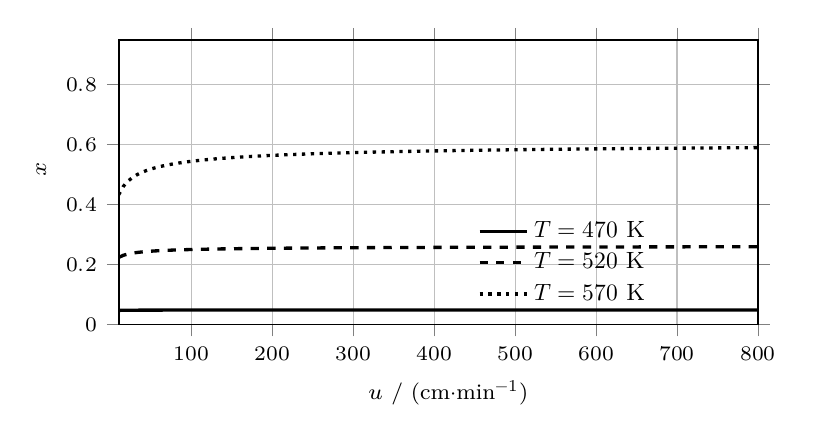
\begin{tikzpicture}
\tikzset{declare function={
  xint(\T)=0.92*(44000000*exp(-9622/\T))/(1+44000000*exp(-9622/\T));
  xext(\u)=2.5*sqrt(\u/30);
  xobs(\u,\T)=1/(1/xint(\T)+1/xext(\u));
}}
\begin{axis}[
  width=\onecolwidth, height=52mm,
  xlabel={线速 $u$ / (cm$\cdot$min$^{-1}$)},
  ylabel={转化率 $x$},
  domain=10:800, samples=140,
  xmin=10, xmax=800, ymin=0, ymax=0.95,
  legend pos=south east,
  legend cell align=left,
  grid=major,
  tick label style={font={\fontsize{7.5}{9}\selectfont}},
  label style={font={\fontsize{8}{9.5}\selectfont}},
  legend style={font={\fontsize{7}{9}\selectfont}, fill=none},
]
\addplot[very thick] {xobs(x,470)};
\addlegendentry{$T=470$~K：曲线水平，外扩散不存在}
\addplot[very thick, dashed] {xobs(x,520)};
\addlegendentry{$T=520$~K：仍有可辨的线速依赖}
\addplot[very thick, dotted] {xobs(x,570)};
\addlegendentry{$T=570$~K：外扩散起作用，趋向平台}
\end{axis}
\end{tikzpicture}
\caption{模型计算：\textbf{接触时间（空速）保持不变}、只改变线速时，转化率随线速的变化
如何判别外扩散控制。读者应看三条曲线的\textbf{形状差异}：低温曲线在整个线速区间水平，
说明速率与线速无关，数据落在本征动力学区；温度升高后曲线左端明显偏低、随线速上升并
逐渐逼近平台，左端即外扩散控制区，右端的平台才是可以取数的区域。\textbf{条件与局限}：
等温、无内扩散（取足够小的粒径）、反应不可逆且远离平衡；模型为串联阻力式
$1/x=1/x_{\text{本征}}+1/x_{\text{外}}$，其中外扩散可达的极限转化率取
$x_{\text{外}}\propto k_m\propto u^{0.5}$、本征可达转化率取 Arrhenius 型有界式
$x_{\text{本征}}=0.92\,A/(1+A)$、$A=4.4\times10^{7}\exp(-9622/T)$；纵轴数值为示意，
不代表任何具体反应体系；三条曲线的温度为 $470$、$520$、$570$~K，绝对位置可整体缩放而
不改变判别结论。\modelmark\figsrc{据 S2 §10.5.4 图 10-20、图 10-21 的判据改绘为模型计算}}
\label{fig:ch10-velocity}
\end{figure}

\begin{figure}[htbp]
\centering
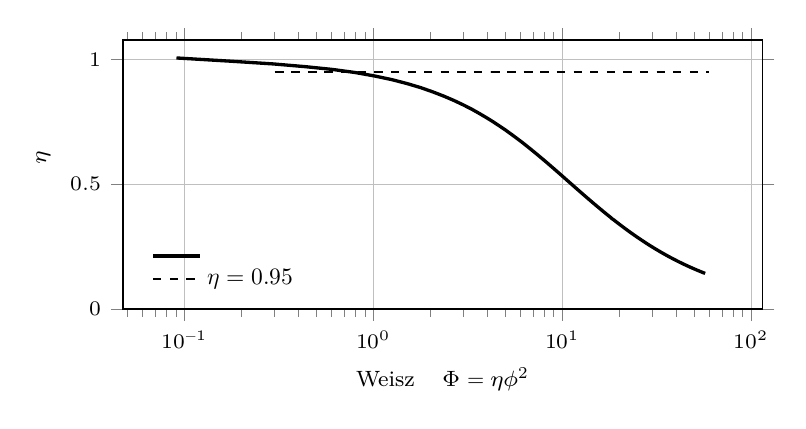
\begin{tikzpicture}
\tikzset{declare function={
  etaWP(\p)=(3/\p)*(1/tanh(\p)-1/\p);
  PhiWP(\p)=etaWP(\p)*\p*\p;
}}
\begin{axis}[
  width=\onecolwidth, height=50mm,
  xmode=log,
  xlabel={Weisz 模数 $\Phi=\eta\phi^{2}$},
  ylabel={有效因子 $\eta$},
  domain=0.3:20, samples=160,
  ymin=0, ymax=1.08,
  legend pos=south west,
  grid=major,
  tick label style={font={\fontsize{7.5}{9}\selectfont}},
  label style={font={\fontsize{8}{9.5}\selectfont}},
  legend style={font={\fontsize{7}{9}\selectfont}, fill=none},
]
\addplot[very thick] ({PhiWP(x)},{etaWP(x)});
\addlegendentry{球形颗粒、一级反应（精确解）}
\addplot[dashed, domain=0.3:60] {0.95};
\addlegendentry{$\eta=0.95$ 参考线}
\end{axis}
\end{tikzpicture}
\caption{模型计算：Weisz 模数与有效因子的关系，用于把式~\eqref{eq:wp} 的判据落到可读的
数值上。读者应看\textbf{曲线与 $\eta=0.95$ 参考线的交点}：交点位于 $\Phi\approx 0.75$
—$1.0$ 之间，即判据取 $\Phi<1$ 时有效因子不低于约 $0.94$；$\Phi$ 再大一个数量级，
$\eta$ 已降到 $0.5$ 以下，此时测得的活化能与级数都不能当本征值用。\textbf{条件与局限}：
曲线由球形颗粒一级反应的精确解 $\eta=(3/\phi)(1/\tanh\phi-1/\phi)$ 与
$\Phi=\eta\phi^{2}$ 数值算出，只适用于等温、一级、球形；其它级数与形状的曲线位置不同，
故原书对二级反应另给 $\Phi<0.3$。\modelmark\figsrc{据 S2 §10.5.2 图 10-12 与 §10.5.4
式（10-131）重算}}
\label{fig:ch10-etaphi}
\end{figure}

\begin{dataflow}
\textbf{「本征动力学数据」的取得流程与失败分支。}
（1）按几何条件设计反应管：内径 $\ge 10d_p$，气固床层长 $\ge 50d_p$（液固为几百倍
$d_p$）。（2）用萘锭传质实验与示踪脉冲返混实验确认装置的无梯度性（无梯度反应器）
或活塞流性（管式反应器）。（3）做实验一（变线速、保持 $W/F$）：转化率出现平台
$\Rightarrow$ 外扩散已排除；用式~\eqref{eq:da} 复核 $Da<0.15/m$。（4）做实验二
（变粒径、保持空速）：转化率出现极限值 $\Rightarrow$ 取极限粒径以下的数据；用
式~\eqref{eq:wp} 复核 $\Phi<1$（二级反应 $<0.3$）。（5）用
式~\eqref{eq:mears-heat} 确认相间温差可忽略。（6）在通过（3）—（5）的温度区间内拟合
速率方程；任一步失败，就只能报告\textbf{表观}速率方程，并注明受控的传递环节。
\src{S2 §10.5.4，书内 p.790—793 / PDF p.279—282}
\end{dataflow}

\begin{pitfall}
\textbf{本节的四个高频误判。}
（1）\textbf{在传质控制区测「本征活化能」，得到偏低的假值。}强内扩散控制下一级反应的
表观活化能约为真实值的一半（$E_{\mathrm{app}}\approx E/2$），表观级数同样被推离真值。
判别方法：看 $E$ 的数值是否随粒径变化——改变粒径而 $E$ 变，说明测的不是本征值；
在内扩散区减小粒径可提高速率，但\textbf{不会}改变真实活化能这一事实，恰是分解二者的
钥匙。\src{S2 §10.4.2，书内 p.772—775 / PDF p.261—264}
（2）\textbf{催化剂装填量过大导致床层温度梯度。}积分反应器中转化率高、反应热稍大就
难恒温；装填量越大、床层越长，轴向温差越大，而速率对温度是指数敏感的，于是「床层平均
温度」变成一个人造量。对策：减小管径、恒温导热介质、惰性稀释、非等比稀释
（入口加大稀释比），必要时改用微分床或无梯度反应器。\src{S2 §10.5.1，书内 p.779—780 /
PDF p.268—269}
（3）\textbf{转化率取点太靠近平衡。}可逆反应的速率中含推动力项 $(c_1-c_2/K_{eq})$，
当 $c_2/c_1\to K_{eq}$ 时推动力趋于零，表观反应级数趋于零、速率趋于零，此时测得的
「级数」与「活化能」都只是分析误差的放大器，与机理无关。取点应保证
$c_2/c_1$ 明显小于 $K_{eq}$，并在报告中给出该比值。
（4）\textbf{产物分析滞后导致非稳态数据错配。}SSITKA、TAP、过渡应答测的都是\textbf{瞬变
曲线}，而色谱一轮分析以分钟计，用它跟瞬变过程对不上：进样阀、管线和检测器死体积会把
阶跃展宽成一个「仪器应答函数」。正确做法是用多通道快速质谱（这正是 SSITKA 与 TAP 都对
检测器提出「时间分辨率高」「电离室距反应器出口 $\le 1$~cm」要求的理由），并先用空白
阶跃测出仪器应答，再把实测曲线与理论曲线对照；色谱只用于测定稳态浓度。
\src{S2 §10.6.3，书内 p.798 / PDF p.287；§10.6.4，书内 p.799 / PDF p.288}
\end{pitfall}

\subsection{非稳态催化过程动力学}

以上讨论主要基于\textbf{稳态过程}。然而在实际催化过程中，催化剂的活性和选择性随反应
时间而变化：反应初期活性逐步上升（如诱导期），反应末期逐步下降（如失活）；也有人为地
周期变动操作条件（温度、浓度、组成）以提高生产能力或改善选择性。在这些非稳态过程中，
反应速率随时间而变化。另一方面，即使体系处于稳态，\textbf{稳态动力学本身也给出不了
吸附态的浓度与寿命}——它只能给出速率对流体相组成的依赖。本节的四个小节分别处理：
活性随时间衰减（积炭失活）、同一条件下的多个定态与振荡、以及两种以同位素与脉冲为工具
的瞬变方法（SSITKA 与 TAP）。\src{S2 §10.6 引言，书内 p.793 / PDF p.282}

\begin{probout}
非稳态方法的价值不在于「更高级」，而在于它测的是\textbf{另一类量}：稳态实验能给出
$r=f(c_i,T)$，却无法回答「表面上现在有多少中间物种、它们待了多久、哪一步最慢」。
本节的落点是三条时间轴——\textbf{秒以下的表面过程}（SSITKA、TAP）、\textbf{分钟到小时的
催化剂失活}（积炭动力学）、\textbf{秒到分的自持振荡}（多稳态与振荡）。选择方法的第一
原则是\textbf{时间尺度匹配}：方法的时间分辨率必须快于所测过程的时间常数，否则得到的
是卷积后的假象。
\end{probout}

\subsubsection{积炭失活动力学}

早在 20 世纪 50 年代就有关于积炭导致催化剂失活的、积炭浓度与时间的指数关系经验式，
但长期难以发展成有严格理论基础的动力学。主要原因有两层：积炭本身是一个复杂过程；
碳沉积与主反应、与扩散相互纠结，难以区分。从来源看，积炭可以是起始反应物本身的副反应
（与主反应\textbf{平行}），也可以从中间产物开始（与主反应构成\textbf{连串}）；从位置看，
碳沉积可以发生在全部活性位上，也可以选择性地发生在某些活性位上；根据扩散模数的大小或
积炭反应的不同，积炭可以发生在孔道外部或内部、颗粒外表面或核心、床层开始端或尾部；
较高积炭量时孔道会有不同程度的堵塞，堵塞程度取决于积炭量、积炭机理与孔结构。由于积炭
活性位的性质尚不清楚、孔结构也难以在几何上严格描述，严格的动力学处理很困难。Froment
等在活性位、催化剂颗粒和反应器\textbf{三个尺度}上建立了动力学方程。
\src{S2 §10.6.1，书内 p.793—794 / PDF p.282—283}

\begin{principle}
\textbf{活性位尺度的积炭失活模型。}以单分子可逆反应
$\mathrm{B_1\rightleftharpoons B_2}$ 为例。当表面反应为速率控制步骤时，按
Langmuir–Hinshelwood（LH-HW）方法，速率方程可写为
\begin{equation}
r=k_1K_1c_L\left(c_1-\frac{c_2}{K_{eq}}\right)
\label{eq:coke-r}
\end{equation}
碳的前体 C 与吸附的 $\mathrm{B_1}$、$\mathrm{B_2}$ 竞争活性位，形成不可逆的
$\mathrm{CL}$ 物种，于是总活性位浓度
\begin{equation}
c_t=c_L+c_1+c_2+c_{CL}
\label{eq:coke-sites}
\end{equation}
按 Langmuir 吸附方程，式~\eqref{eq:coke-sites} 可写成
\begin{equation}
c_t-c_{CL}=c_L(1+K_1c_1+K_2c_2)
\label{eq:coke-langmuir}
\end{equation}
把式~\eqref{eq:coke-langmuir} 代入式~\eqref{eq:coke-r}，得
\begin{equation}
r=\frac{c_t-c_{CL}}{c_t}\cdot
\frac{k_1K_1\left(c_1-c_2/K_{eq}\right)}{1+K_1c_1+K_2c_2}
=\varphi\,r_{\text{fresh}},\qquad
\varphi\equiv\frac{c_t-c_{CL}}{c_t}
\label{eq:coke-activity}
\end{equation}

\textbf{这个等式只有一种正确读法，代入时不要多做一步除法}：右边第一个因子
$\varphi=(c_t-c_{CL})/c_t$ 是\textbf{无量纲的活性系数}（$\varphi=1$ 为未失活），
第二个因子才是\textbf{速率}（单位与 $r$ 相同）。两者是\textbf{相乘}关系，
$c_t$ 只在 $\varphi$ 里出现一次。逐项核对：

- \textbf{与直接代入恒等}：式~\eqref{eq:coke-langmuir} 给出
  $c_L=(c_t-c_{CL})/(1+K_1c_1+K_2c_2)$，代回式~\eqref{eq:coke-r} 立即得到上式，
  故式~\eqref{eq:coke-activity} 与式~\eqref{eq:coke-r} 是同一个方程，增减任何因子都会破坏恒等。
- \textbf{未失活极限}：$c_{CL}=0$ 时 $\varphi=1$，$r$ 回到新鲜的
  $r_{\text{fresh}}=k_1K_1(c_1-c_2/K_{eq})/(1+K_1c_1+K_2c_2)$；$c_{CL}=c_t$
  时 $\varphi=0$、$r=0$，两端都正确。
- \textbf{对总位点浓度的依赖}：$c_{CL}$ 固定时
  $r\propto(c_t-c_{CL})$；若 $c_{CL}$ 与 $c_t$ 同比例变化（$\varphi$ 不变），
  则 $r\propto c_t$。$c_t$ 翻倍、$c_{CL}$ 不变时速率不会只翻一倍，
  而是按 $(c_t-c_{CL})$ 线性增加——这正是「活性系数」与「绝对速率」必须分开的原因，
  也是该模型给不出绝对速率、只能给出相对失活描述的根本局限。

活性位的初始积炭覆盖速率 $r_{s0}$
\textbf{不能直接测量}，只能由得到的积炭形成速率 $r_C$ 换算，换算中还要用到积炭的相对
分子质量 $m_C$ 与单个活性位上的积炭量 $\gamma$：
$r_{s0}=r_C/(m_C\gamma c_t)$。
\tocheck{未对照原页面图像：$r_{s0}$ 的换算式中 $\gamma$ 与 $c_t$ 的位置无法从 OCR 判定
（OCR 仅给出 $r_C/(c_t m_C)$）；式~\eqref{eq:coke-activity} 分子中\textbf{不应}再乘一个
$c_1$——$c_1$ 已经出现在 $(c_1-c_2/K_{eq})$ 里，再乘一次即重复计入，OCR 是否多出这一
因子未能判读。}
\src{S2 §10.6.1，书内 p.794 / PDF p.283}
\end{principle}

活性位数目的减少主要由积炭机理和生成速率决定。对于\textbf{平行}积炭反应
$r_C=c_tk_{C1}K_1c_1/(1+K_1c_1+K_2c_2)=r_{C0}\varphi_C$；对于\textbf{连串}积炭反应
$r_C=c_tk_{C2}K_2c_2/(1+K_1c_1+K_2c_2)=r_{C0}\varphi_C$。若积炭与主反应在同一活性位上
进行、并且速率决定步骤涉及相同数目的活性位，则 $\varphi_C=\varphi_1$，即积炭系数等于
主反应的失活系数。若主反应的活性位数为 $n_1$、积炭的活性位数为 $n_C$，则

\begin{equation}
\varphi_1=\left(\frac{c_t-c_{CL}}{c_t}\right)^{n_1},\qquad
\varphi_C=\left(\frac{c_t-c_{CL}}{c_t}\right)^{n_C}
\label{eq:coke-phi}
\end{equation}

式~\eqref{eq:coke-activity} 通过 $c_{CL}$ 求解 $\varphi_C$ 与 $\varphi_1$，对活性位被
覆盖而失活的情形有清晰的物理意义。该模型尽管没有考虑孔道堵塞和温度变化，对一些简单
积炭失活动力学研究仍有指导意义——例如甲烷蒸气重整中的积炭过程（积炭主要源于甲烷裂解
反应）；但对石油炼制和化工中的积炭反应要复杂得多，其动力学研究还有待深入。
\src{S2 §10.6.1，书内 p.795 / PDF p.284}

对\textbf{催化剂颗粒尺度}的积炭动力学，浓度分布与孔的网络结构必须考虑，Froment 等用
阈值理论和有效介质近似建立了相应方程；\textbf{反应器尺度}的积炭失活过程更为复杂，
可参考文献。在实用上，通常给出的是催化剂瞬时活性与积炭量的关系（比活性与时间的关系对
机理研究、反应器设计和催化剂再生更实用），已有线性式、指数式与双曲线式等不同经验式。
例如 Nam 和 Kittrell 把积炭分为单层覆盖（占据活性位）与多层覆盖（不另占活性位），并
设定多层积炭生成速率对反应物 $\mathrm{B_1}$ 的分压 $p_1$ 和单层积炭浓度 $c_\alpha$
均为一级：

\begin{equation}
\frac{\delta c_\beta}{\delta t}=k_\beta c_\alpha p_1
\label{eq:multilayer-coke}
\end{equation}

由此推出总积炭量 $c_\sum$ 与活性系数 $k_t$ 的关系

\begin{equation}
c_\sum=q_1(1-k_t)-q_2\ln k_t,\qquad
q_1=m_CS_0-q_2,\qquad
q_2=\frac{k_\beta m_CS_0(1+K_1p_1+K_2p_2)}{k_\alpha K_1}
\label{eq:nam-kittrell}
\end{equation}

式中 $c_\alpha$、$c_\beta$、$c_\sum$ 分别为单层、多层和总积炭量，$k_\alpha$ 与
$k_\beta$ 分别为单层和多层碳生成速率常数，$k_t$ 为活性系数。原书指出：在某一参数关系下
$k_t$ 与 $c_\sum$ 呈\textbf{指数关系}，在另一关系下呈\textbf{线性关系}；该模型同样未
考虑孔道堵塞与温度变化，也未考虑表面反应速率控制以外的其它机理，但对\textbf{微分反应器}
上的失活动力学数据处理非常有用。
\tocheck{未对照原页面图像：式~\eqref{eq:nam-kittrell} 中 $\ln k_t$ 项的正负号，以及
「$q_1$ 与 $q_2$ 何种相对取值给出指数关系、何种给出线性关系」——OCR 在此处丢失了两个
关系符号，无法判定。}\src{S2 §10.6.1，书内 p.795—796 / PDF p.284—285}

\textbf{非恒温条件下的失活动力学。}解析时需在物料衡算方程和失活方程中引入 Arrhenius
数，在热平衡方程中引入主反应与积炭反应的热效应。以放热反应为例，催化剂球形颗粒中
$\mathrm{B_1}$ 的浓度与温度分布可用一组\textbf{无因次方程组}描述（两个二阶方程分别给出
无因次浓度与无因次温度，源项中含失活参数与热效应参数），失活速率方程则把无因次活性
系数的时间导数写成两个并行／连串积炭函数之和；通过数值计算可求出平行积炭与连串积炭中
不同反应时间颗粒内温度与活性系数的径向分布，以及颗粒的\textbf{非恒温有效因子}。
这套分析的前提是\textbf{低积炭}，即孔道无明显堵塞；积炭量高、孔道堵塞严重影响扩散时，
动力学中必须考虑失活对扩散的影响。\tocheck{未对照原页面图像：该无因次方程组与失活速率
方程的具体形式（$\nabla^{2}$ 项的系数、失活方程右端两项的权重 $k_{f1}/k_{f2}$）在 OCR
中不完整，故此处只叙述结构与前提，不抄录方程。}
\src{S2 §10.6.1，书内 p.796 / PDF p.285}

实际催化过程中的失活动力学更为复杂，通常只能用经验式表达。例如重油催化裂化，组分非常
复杂、催化剂活性位强度分布范围很宽，即使简化处理，也会发现\textbf{积炭的反应级数从初期
的高级数向后期的低级数过渡}。此外，上述解析都假定\textbf{反应动力学本身不受失活影响}；
虽有学者从理论上论证非均匀表面上的失活动力学不宜采用这一假定，但由于表面非均匀性不易
处理、且该假定在一些失活动力学处理中应用成功，用它处理实际问题仍是可行的。
\src{S2 §10.6.1，书内 p.796 / PDF p.285}

\begin{crosscheck}
积炭失活的数据必须与\textbf{稳态动力学}分开拟合、再互查：（1）式~\eqref{eq:coke-r}—
\eqref{eq:coke-activity} 假定主反应的速率方程形式（含 $K_1$、$K_2$）在失活过程中不变，
这只在\textbf{活性位数按同一比例减少}时成立——若积炭选择性地覆盖某类活性位，
$K_1/K_2$ 也会变，此时「活性系数」不再是单一标量。（2）检验办法是把不同积炭量下的
稳态速率方程分别拟合，看 $K_i$ 是否漂移；漂移则说明失活不是简单的位点计数问题。
（3）式~\eqref{eq:nam-kittrell} 一类活性-积炭量关系式是对\textbf{微分反应器}数据最有用，
与积分床数据互查时须先做积分校正。
\end{crosscheck}

\subsubsection{催化反应动力学中的多稳态与振荡}

催化反应的稳态指体系的质量、能量流动处于平衡状态，各项参数不随时间改变。
\textbf{多稳态}的提出最初基于对强放热反应的反应器解析：在同一入口温度下，绝热反应器
可以在两个定态下操作。它在催化剂颗粒、全混流反应器、进出口自换热反应体系等不同尺度上
都存在。多稳态最初主要归因于传质过程，但在\textbf{恒温且无传质影响}的条件下仍会出现：
例如 Pt/Al$_2$O$_3$ 催化剂上的 CO 氧化，在相同恒温条件下 CO 转化率可以恒定在约 $10\%$
（「低稳态」），也可以恒定在约 $40\%$（「高稳态」），\textbf{取决于催化剂的预处理条件}。
若系统从高稳态自动转入低稳态，并随时间延长自动由低稳态转入高稳态，就在两个稳态之间
形成持续性\textbf{振荡}。例如 CO 在 Pt/Al$_2$O$_3$–SiO$_2$ 上的氧化反应中反应速率随
CO 浓度振荡；在低 CO 分压下反应对 CO 是一级，在高分压下对 CO 是\textbf{负一级}。
\src{S2 §10.6.2，书内 p.796—797 / PDF p.285—286}

振荡行为在氢气、氨气、烃类、甲醇和乙醇氧化、F–T 合成、乙烯和硝基苯加氢等反应中广泛
存在。研究它有两重意义：既揭示影响催化剂性能的因素与非稳态操作下的潜在危险，
也可以\textbf{利用振荡提高催化反应效率}（例如通过调节温度和组成强制振荡以提高转化率）。
对 Pt 上 CO 氧化振荡的研究，揭示了 Pt 表面重构、具有高 O$_2$ 黏结系数的表面缺陷、
CO 表面覆盖度变化等一系列影响催化剂性能的因素。
\src{S2 §10.6.2，书内 p.797 / PDF p.286}

\begin{principle}
\textbf{振荡的数学描述。}原理上，振荡可用总包反应中物种的表面浓度 $c_i$ 随时间变化的
一组微分方程描述，其速率方程可由基元步骤得到：
\begin{equation}
\dd c_i/\dd t=F_i(c_j,\,p_k)
\label{eq:osc-ode}
\end{equation}
式中 $c_j$ 为所有的态变量，$p_k$ 为外部参数（温度、分压等）。然而对实际体系，空间均一性
是不可能的，甚至对单晶表面也是如此。对固定床反应器，催化反应振荡是多个因素\textbf{同步
化}的结果，同步化因素包括：催化剂、载体或气相的传热；表面振荡导致的分压变化；吸附物种
的表面扩散或表面结构的转变。因此式~\eqref{eq:osc-ode} 需修正为
\begin{equation}
\partial c_i/\partial t=F_i(c_j,\,p_k)+D_i\,\frac{\partial^{2}c_i}{\partial r^{2}}
\label{eq:osc-ode-diff}
\end{equation}
式中 $D_i$ 为普适扩散系数，$r$ 为空间坐标。一般每个反应均有其自己的振荡机制，普适化
只在一定程度上可行。\src{S2 §10.6.2，书内 p.797 / PDF p.286}
\end{principle}

\begin{pitfall}
\textbf{不要把振荡区的数据当稳态数据拟合。}（1）多稳态意味着\textbf{同一操作条件对应
两个以上的速率值}，若实验不记录预处理历史与升降温路径，同一组 $(T,\,p_i)$ 会给出互相
矛盾的速率，看起来像「实验不可重复」。（2）式~\eqref{eq:osc-ode-diff} 提示：固定床中的
振荡是同步化现象，因此\textbf{反应器尺度的振荡周期与颗粒尺度的本征周期不等}，用床层
出口的振荡周期去反推表面基元步骤的时间常数是危险的。（3）工程上的正面用法是「利用」：
强制周期操作（周期进料、周期变温）可以改变时均转化率与选择性，这时应以\textbf{时均
性能}与稳态性能对比，而不是逐点比较。
\src{S2 §10.6.2，书内 p.797 / PDF p.286}
\end{pitfall}

\subsubsection{非稳态方法一：稳态同位素瞬变动力学分析（SSITKA）}

\term{SSITKA}{steady state isotopic transient kinetic analysis}{稳态同位素瞬变动力学
分析}是\textbf{同位素示踪技术}与\textbf{动态瞬变技术}的结合，可分为稳态与非稳态两类
实验：非稳态实验主要用于获得反应机理的信息，而稳态实验则融瞬变与稳态实验于一身，
在获得定性信息的同时还能获得反应中间物的\textbf{定量}信息。SSITKA 一般采用
\textbf{质谱}作为检测手段，通过检测未反应的反应物和反应产物的瞬变响应，获取反应机理和
原位动力学信息。原位红外或核磁共振在观察催化剂表面方面有独特优势，可以直接观察反应
过程中表面与表面上吸附物种的变化；把 SSITKA 与 FTIR 或 NMR 结合，利用瞬变红外或瞬变
核磁共振光谱，不仅可以研究表面动态反应和鉴别表面吸附中间物种，还可以通过\textbf{同位素
位移效应}正确表征表面中间物种——包括其化学结构和表面覆盖度，并可分辨吸附的反应物种与
非反应物种，弥补了单纯用质谱检测的不足。
\src{S2 §10.6.3，书内 p.797 / PDF p.286}

\begin{measure}
\textbf{SSITKA 的装置与操作（原书图 10-23）。}装置包括\textbf{气路控制部分}、\textbf{反应
器}和\textbf{质谱在线分析系统（MS）}，并常配一台色谱仪以测定反应物和产物的浓度。
气路控制部分最重要的是切换气路的\textbf{四通阀}：切换时应尽量不对体系的压力、气体组成
和流动产生干扰，以保持原有稳态。反应器采用\textbf{理想反应器}，如活塞流反应器或全混流
反应器；尤其是活塞流反应器体积小、操作简单，短床层具有无轴向扩散的特点。检测用的质谱仪
是 SSITKA 的核心，要求能够\textbf{多通道连续快速分析且时间分辨率高}。
\textbf{操作流程}：实验前，反应物与同位素标记的反应物两路气体需要连续流动；然后用四通阀
切换气路，使同位素标记的反应物通过反应器并在催化剂表面反应生成同位素标记的（中间）
产物，用质谱仪跟踪其\textbf{替代过程}及其变化曲线。
\src{S2 §10.6.3，书内 p.798 / PDF p.287}
\end{measure}

\begin{dataflow}
\textbf{从 SSITKA 曲线到动力学参数。}（1）对瞬变曲线积分，可获得两个基本参数：
\textbf{表面中间物种的停留时间}与\textbf{其量}。（2）若用化学吸附测定出催化剂表面暴露的
金属原子数，就可以由中间物种的量算出\textbf{表面覆盖度}。（3）若表面进行的化学反应能够
假定为\textbf{拟一级}，那么很容易求得拟一级反应速率常数。（4）SSITKA 实验还能测量与
假定反应机理相关的一些参数。利用 SSITKA 研究过的典型催化反应有：氨合成、CO 加氢、
乙烷裂解、甲烷活化和 CO 氧化等。\src{S2 §10.6.3，书内 p.798—799 / PDF p.287—288}
\end{dataflow}

\begin{pitfall}
\textbf{SSITKA 的三条使用边界。}（1）\textbf{必须有可标记元素}：它测的是同位素替代过程，
对不含可交换标记原子的反应无法施用。（2）\textbf{切换本身必须是「无扰动」的}：四通阀的
死体积、切换瞬间的压力波动与流量扰动都会直接进入瞬变曲线，把停留时间算长；这正是原书
强调「切换时应尽量不对体系压力、气体组成和流动产生干扰，保持原有稳态」的原因。
（3）\textbf{质谱的碎片与同位素峰重叠}：标记产物的母峰与碎片峰常与未标记物种的部分峰
重叠，若不做碎片校正，替代曲线会被人为拉长——常规做法是同时采集多个 $m/z$ 通道并用
纯物质标定碎片比。\tocheck{未对照原页面图像：碎片重叠与校正属常规质谱实践，原书未展开，
此条为补充，供回查。}\src{S2 §10.6.3，书内 p.798 / PDF p.287}
\end{pitfall}

\subsubsection{非稳态方法二：产物瞬态分析（TAP）}

\term{TAP}{temporal analysis of products}{产物瞬态分析}是一种研究多相催化动力学的新
技术，能够用于真空脉冲-应答实验、程序升温脱附／反应实验以及常压稳态和瞬态实验，
既可以研究模型催化剂，也可以研究工业催化剂。\src{S2 §10.6.4，书内 p.799 / PDF p.288}

\begin{measure}
\textbf{TAP 的四个组成部分与关键参数（原书图 10-24）。}（1）\textbf{高真空下的微反应器}：
可以只填充催化剂，也可以在两端填充惰性填料、中间填充催化剂——后者称为\textbf{三区
反应器}，优点是可以获得更多的信息并进一步简化数学处理；如果催化剂床层填充得非常薄，
可以认为是全混流反应器，使数学处理更简化且床层状态更均一。（2）\textbf{产生窄脉冲的
电磁脉冲发生器}：时间宽度可到 $10^{-4}$~s 数量级，弛豫时间可以在 $10^{-4}$—$10^{3}$~s
之间变化；如此短的脉冲使 TAP 能够检测到毫秒级的化学反应。（3）\textbf{质谱检测器}：
一般采用四极质谱仪检测反应物、中间产物和最终产物的化学组成；一般电离室与反应器出口间
距离不大于 $1$~cm，背景压力小于 $10^{-6}$~Pa，具有非常高的灵敏度。（4）\textbf{自动
控制／数据处理系统}。\textbf{脉冲进样量的量级}：反应物可以控制在 $10^{10}$—$10^{15}$ 个
分子，只占催化剂表面活性位数量的\textbf{百万分之一}，因此不会对催化剂的表面状态产生
影响；检测到的结果是催化剂表面恒定状态下反应分子与表面的作用，反映的是\textbf{本征的
相互作用}。又由于进样量非常少，分子对流传输消失，\textbf{仅有 Knudsen 扩散}。
\src{S2 §10.6.4，书内 p.799 / PDF p.288}
\end{measure}

\begin{dataflow}
\textbf{从 TAP 曲线到参数：标准曲线比较法。}TAP 得到的是反应物、中间产物和最终产物的
气流随时间变化的曲线；通过分析与数学处理得到动力学和传递方面的信息。目前已经发展出
处理下列情形的\textbf{理论标准曲线}：仅 Knudsen 扩散、扩散 + 不可逆反应、扩散 + 可逆
吸附、快速吸附-慢脱附、快速吸附-脱附等。把实验曲线与标准曲线比较，就可以分析判断并
测量\textbf{扩散系数、不可逆吸附／反应、可逆吸附}等参数，从而获得催化剂的物理化学和
动力学状态的信息。TAP 已用于氧化物上的吸附和脱附、氧活化、丙烯选择氧化、甲醇氧化／
氨氧化、丁烷氧化、甲烷转化等研究，给出吸附、脱附、扩散等参数以及反应网络和机理的新
论据。\src{S2 §10.6.4，书内 p.800 / PDF p.289}
\end{dataflow}

\begin{crosscheck}
\textbf{三类瞬变方法的时间尺度与信息分工，是本节最需要记住的一张表。}
TAP 的脉冲宽度在 $10^{-4}$~s 量级、弛豫时间 $10^{-4}$—$10^{3}$~s，因此它能分辨
毫秒级过程且几乎不扰动表面；SSITKA 的典型时间窗是表面中间物种的停留时间（秒量级），
且必须在\textbf{稳态背景}下做同位素切换；过渡应答法施加的是浓度阶跃，其应答衰减在
秒到分量级；而积炭失活与振荡分别是分钟—小时与秒—分尺度。\textbf{方法能不能用，首先
取决于它比所测过程快多少}。三者与稳态方法的分工见表~\ref{tab:ch10-transient}。
\end{crosscheck}

\begin{table}[tbp]
\centering
\caption{稳态与非稳态动力学方法的时间尺度与信息分工。看第二列：\textbf{方法的时间分辨率
必须快于所测过程的时间常数}，否则得到的是与仪器应答卷积后的假象；看第三、四列：
「给不出」一栏决定了任何单一方法都不能独立定出机理。\src{据 S2 §10.5.3—§10.5.4、
§10.6.1—§10.6.4，书内 p.788—800 / PDF p.277—289 整理。}}
\label{tab:ch10-transient}
{\srcsize
\begin{tabularx}{\twocolwidth}{@{}p{21mm}p{26mm}p{52mm}X@{}}
\toprule
方法 & 特征时间尺度 & 能给出什么 & 给不出什么 \\
\midrule
稳态动力学 & 达稳态后取数（分钟—小时） & 速率方程、速率常数、表观活化能、反应级数、
吸附平衡常数的组合、选择性的宏观规律 & 吸附态浓度与寿命、中间物种的身份、速率控制步骤的
直接证据；无法区分「$K$ 大而覆盖度高」与「$K$ 小而覆盖度低」 \\
过渡应答（浓度阶跃） & 秒—分（应答衰减） & 吸附量（应答曲线下的阴影面积）、吸附与
脱附速率、由产物应答的即时性判断速率控制步骤、由降零实验判断基元步骤可逆性 & 绝对覆盖度
（需先测活性位数）；解析依赖假定的基元步骤网络，网络错则参数系统性偏移 \\
SSITKA & 秒量级（表面中间物种停留时间） & 中间物种的\textbf{停留时间与量}；配化学吸附
得覆盖度；拟一级假定下得拟一级速率常数；与原位 IR／NMR 联用可得中间物种结构与同位素
位移信息 & 毫秒以下过程；必须存在可标记元素；切换瞬间的压力与流量扰动会直接污染停留
时间 \\
TAP & 脉冲 $10^{-4}$~s；弛豫 $10^{-4}$—$10^{3}$~s & 仅 Knudsen 扩散下的扩散系数、
不可逆吸附／反应、可逆吸附参数；反应网络与机理新论据；几乎不扰动表面（脉冲分子数只占
表面活性位的百万分之一） & 常压稳态速率与高转化率选择性；对流传输消失，故不能代表工业
条件下的相间传递 \\
程序升温脱附／反应（TAP 的升温模式，即 TPSR 类实验） & 由升温速率决定，通常为分钟级
& 表面吸附态与中间物\textbf{随温度的转化序列}，以及产物与活性位的对应关系 & 单独的定量
动力学参数——温度与覆盖度同时变化，必须借助模型反演，或与 SSITKA／稳态数据联合定参
\tocheck{未对照原页面图像：原书只在 TAP 的能力列表中列出「程序升温脱附／反应实验」，
未给出升温速率范围；本行的分钟级时间尺度与信息表述属常规实践归纳，需回查原书或另找
出处。} \\
积炭失活 & 分钟—小时—天 & 活性系数随积炭量的衰减规律（线性／指数／双曲线型）；三段
尺度（活性位、颗粒、反应器）的失活模型 & 初始积炭覆盖速率 $r_{s0}$ 不能直接测，只能由
$r_C$ 换算；高积炭下的孔道堵塞须另行处理 \\
多稳态与振荡 & 秒—分（振荡周期） & 同一操作条件下的多个定态与自持振荡；表面重构、
覆盖度变化等机理线索；强制周期操作可改变时均性能 & 用出口振荡周期反推表面基元步骤的
时间常数（固定床中是同步化结果）；也不能当作稳态速率数据使用 \\
\bottomrule
\end{tabularx}}
\end{table}

\subsection{结论}

多相催化动力学已发展成为内容非常丰富的交叉学科，近五十年来在\textbf{宏观-介观-微观}
不同尺度上都有不同程度的发展。宏观尺度上的动力学是催化剂性能最直接的表征手段，
但其所能表征的性能与反应的复杂程度直接相关：对\textbf{简单反应}，速率方程、速率常数、
活化能、反应级数及吸附平衡常数等可以较准确而全面地表征；对\textbf{复杂反应}，可通过
反应网络的解析求出催化剂上初级和次级反应的速率常数，从而在更深层次认识催化反应的本质。
在多相催化反应中，\textbf{传递过程也是催化剂的一个重要性能}，对实际催化过程尤其如此。
宏观多相催化动力学还为催化过程提供了数学模型：由于实验技术、分析方法和数值模拟的发展，
所得模型基本可以准确地反映温度、压力和空速等工艺参数对催化反应速率、转化率和选择性的
影响规律，是催化反应器设计和过程优化的基础与手段。此外，宏观多相催化动力学也有助于
催化剂设计及性能优化，以及催化反应机理等基础认识的发展。
\src{S2 §10.7，书内 p.800—801 / PDF p.289—290}

\begin{crosscheck}
把本章三条线索接起来：\textbf{分片 a} 给出「RDS + 吸附平衡 → 速率方程」的形式框架；
\textbf{分片 b} 给出「传递是否限制」的判据与有效因子；\textbf{本分片}给出「怎样用反应器
和实验把二者分开测量」，以及稳态方法给不出的那部分信息如何由非稳态方法补上。任何一条
速率方程在报告时都应同时交代三件事：\textbf{在哪个动力学区取得}（本征／内扩散／外扩散）、
\textbf{传递判据是否通过}（$Da$、$\Phi$、Mears 判据）、\textbf{吸附参数是否独立验证过}
（过渡应答、SSITKA 或 TAP）。缺任何一项，方程就只能作为经验拟合式使用。
\end{crosscheck}

\srcnote{本分片覆盖 S2（下册）第 10 章 §10.5（动力学测定方法和实验装置，含
§10.5.1 实验室反应器、§10.5.2 内扩散参数的测定、§10.5.3 过渡应答法、§10.5.4 本征
动力学区的确定和排除传递过程干扰）、§10.6（非稳态催化过程动力学，含 §10.6.1 积炭失活
反应动力学、§10.6.2 多稳态与振荡、§10.6.3 SSITKA、§10.6.4 TAP）与 §10.7 结论，
源页面为书内 p.779—806 / PDF p.268—295。表~\ref{tab:ch10-reactor} 据原书表 10-3 与
§10.5.1 正文整理，其中「浆态（液固）」一行为补充；图~\ref{fig:ch10-velocity} 与
图~\ref{fig:ch10-etaphi} 为模型计算图，非原书插图复制。公式的重建与存疑点已在正文中
以 \tocheck{} 逐处标明。}
}{}
\IfFileExists{chapters/parts/ch10-d.tex}{\input{chapters/parts/ch10-d}}{}
\IfFileExists{chapters/parts/ch10-e.tex}{\input{chapters/parts/ch10-e}}{}
}{}
\IfFileExists{chapters/ch11.tex}{% chapters/ch11.tex —— 第 11 章 电化学催化研究方法
% 装配层：只负责按顺序引入各分片。分片缺失时跳过，便于增量成书。
% 分片文件：chapters/parts/ch11-{a..e}.tex
%
% 【2026-09-29 调序】原为 a→b→c→d，有两处结构问题：
%   (1) 分片 d = §11.5.1 阻抗谱基本原理（依源文本 p.855—861 写成），却被排在
%       分片 c（§11.5 后半与 §11.6 原位谱学）之后，于是成书里 §11.6 排在
%       §11.5.1 之前，而分片 c 开篇写「阻抗的基本定义……写在上文 §11.5.1」——
%       在成书里这是假陈述；
%   (2) \subsection 按出现顺序自动编号，§11.5.1 会拿到比 §11.5 大的号。
%   现改为 a→b→d→c→e：d（原理）紧接 b（§11.4）之后、c（§11.5 应用与 §11.6）
%   之前，指代方向与前后顺序恢复正确。**注意：编号与原书不再一一对应**——成书为 §11.5 阻抗谱基本原理、§11.6 电化学阻抗谱（原书 §11.5，仅其应用部分）、§11.7 电化学原位谱学（原书 §11.6）。要完全对齐须把分片 d 的标题降为 \subsubsection 并入分片 c 的 §11.5。。分片 d 不含 \chapterstart（章计数器
%   由分片 a 唯一推进），故调序不会影响章号。

\IfFileExists{chapters/parts/ch11-a.tex}{% ================================================================
%  chapters/parts/ch11-a.tex
%  第 11 章  电化学催化研究方法（分片 a）
%  源：S2（下册）第 11 章 11.1—11.2.3，书内 p.807—832 / PDF p.296—321
%  范围：11.1 电化学基本原理；11.2 控制电势的研究方法（至 11.2.3）
%  不含：11.3 及以后（控制电流、整体电解、流体动力学、阻抗、现场谱学）
% ================================================================

\chapterstart{电化学催化研究方法}%
{本章回答：怎样用电势和电流这两个可观测量，把电极反应的本征活性从传质、双电层、
溶液电阻等非本征因素中剥离出来。导读主线只有一条——\textbf{电极反应的总速率由传质与
电荷转移两步串联决定}，11.1 建立描述这两步的方程，11.2 的每一种控制电势方法，本质上
都是在实验上设法单独固定其中一步、观测另一步。全章按「基本原理（11.1）→ 控制电势的
研究方法（11.2）→ 控制电流、整体电解与流体动力学方法（11.3 起）」展开。}
\label{ch:11}

\subsection{电化学基本原理}

\subsubsection{电化学与催化过程关系}

电化学以化学反应中的电子转移以及外加电场中的化学反应为研究对象\src{S2 §11.1.1，
书内 p.809 / PDF p.297}。它与催化化学的交集就是\textbf{电催化}：既是用催化剂提升反应
速率的电化学过程，又是以电能为能量形式的催化过程。二者其实可以统一——电极本身就是
催化剂，改变电极种类或电极表面修饰状态，就能改变反应的速率、选择性和方向性；只有
这类「通过改变电极材料或表面状态来调控反应」的电极，才被称为电催化剂。

两个学科的关注点不同，落到数据分析上会得到不同的结论：催化视角看的是电催化剂如何
降低活化能垒、如何催化能量转化过程；电化学视角看的是界面电场、电解质组成、以及参与
反应的分子或离子被活化后反应速率如何提升。同一个活性数字，两个视角的解释并不相同，
这一点在读到「本征活性」类结论时必须追问研究者用的是哪一套语言。

\begin{probout}
电化学催化实验的可观测量只有两个：\textbf{流过工作电极的电流或电量}，以及\textbf{工作
电极相对参比电极的电势}。所有动力学参数都必须从这两个量的关系中反推。反推的前提是：
电流里不混入非法拉第过程，电势里不混入未补偿的溶液电阻降，传质速率已知或已被排除，
并且电势的参照点（参比电极）和面积基准（几何面积还是真实面积）都被明确交代过。
这四条前提缺任何一条，得到的速率常数和 Tafel 斜率都不可比。
\end{probout}

\subsubsection{电化学涉及的基本概念}

这组概念的用处是给后面的公式划定符号与判据的边界，其中最容易混淆的是\textbf{电势}
类的三个词：平衡电势、过电位、开路电势。

\paragraph{导体、半导体与绝缘体} 按电阻率 $\rho$ 划分：$\rho<\qty{1}{\milli\ohm\centi\meter}$ 为
导体（金、银、铜、铝、铁、电解液、石墨），$\rho>\qty{1}{\giga\ohm\centi\meter}$ 为绝缘体（云母、
橡胶、石英、陶瓷），介于两者之间为半导体（硅、锗、\ce{TiO2}、\ce{GaN}）
\src{书内 p.810 / PDF p.298}。对催化实验的直接含义是：电解液必须导电，但催化剂载体
（如氧化物、碳）可以处于半导体区，其导电性会随电势变化，这会带来额外的、与催化
无关的电流--电势非线性。

\paragraph{电解质与电解液} 电解质是在水溶液中或熔融态能导电的化合物，其导电来自荷电
溶剂化离子在电场下的定向迁移；电解质本身不一定导电，按是否完全电离分为强、弱电解质，
而溶解度大小与强弱无关。电解质并非都是液体：聚合物锂离子电池和质子交换膜燃料电池
使用的就是固体有机电解质。

\paragraph{电极} 按材料分为金属电极、氧化物电极、固体难溶盐电极等；按功能分为工作
电极、对电极、参比电极、离子选择电极。电极的作用是连接电解液与外电路，并在其表面或
近表面界面发生电化学反应。催化研究关心的是工作电极，但\textbf{没有对电极和参比电极的
明确交代，工作电极上的数据无法解释}。

\paragraph{活度、离子氛与电迁移} 溶液中的离子与其周围离子形成相对规律的离子排布区，
称为离子氛。离子到达电极表面发生反应前需从离子氛中剥离，要耗费能量，因此溶液中离子的
自由能与反应活性都略低于自由离子。为描述实际溶液与理想溶液的偏离引入\textbf{活度}：
它是离子相对理想溶液浓度的有效值。离子氛随浓度增大而变大，故活度随浓度增大而减小；
无限稀溶液中离子可近似为自由离子。电解质本体中离子在电场下的定向移动称为\textbf{电迁移}；
电极表面液层中则因部分离子持续反应造成浓度差，驱动离子\textbf{扩散}。扩散和电迁移
共同完成电活性物质的传递，对应电流也分为扩散电流与迁移电流。电极近表面电活性物质的
流量决定反应速率，从而控制外电路电流。

\paragraph{电势的三种含义} 这三个词在催化文献里最常被混用，必须分清：

\begin{itemize}
\item \textbf{平衡电势} $E_{\mathrm{eq}}$：给定温度、压力和\textbf{全部组分活度}下，
  电极上氧化与还原两个方向速率相等、净电流为零时的电势。它是一个由热力学确定的量
  （Nernst 方程给出），与电极材料无关，只与电对和活度有关。
\item \textbf{过电位（超电势）} $\eta=E-E_{\mathrm{eq}}$：实际电极电势偏离平衡电势的
  量，是驱动净反应的「额外推动力」，符号与大小同时编码了动力学信息。$\eta$ 只对确定的
  $E_{\mathrm{eq}}$ 才有定义；讨论 $\eta$ 前必须先说明用什么电对、什么活度算出的
  $E_{\mathrm{eq}}$。
\item \textbf{开路电势} OCP：外电路断开（无净电流）时测得的工作电极电势。它\textbf{等于}
  平衡电势只在电极表面处于热力学平衡时成立；催化研究中电极表面常被吸附物、氧化物层
  或混合电位占据，此条件下 OCP 是一个\textbf{混合电位}，与任何单一电对的
  $E_{\mathrm{eq}}$ 都不相等，因而不能用来计算 $\eta$。
\end{itemize}

\begin{pitfall}
把 OCP 当平衡电势、直接用它算过电位，是电催化文献里最高频的错误之一。判据很简单：
若在该 OCP 处体系的净电流为零是因为\textbf{正逆两个方向的同一反应}速率相等，OCP 才是
平衡电势；若净电流为零是\textbf{两个不同反应}（如氧还原与铂氧化）各自贡献正负电流相消，
那它是混合电位。区分办法是在 OCP 附近做微扰，看响应是容性还是可通过极化曲线外推。
\end{pitfall}

\subsubsection{电势和电池热力学}

电势差推动电子在电路中定向移动；恒温恒压下，若系统的非膨胀功只有电功，则

\begin{equation}
(\Delta_{\mathrm{r}}G)_{T,p}=-nEF
\label{eq:gibbs-emf}
\end{equation}

式中 $n$ 为反应输出电荷的物质的量，$E$ 为可逆电池的电动势，$F$ 为法拉第常量
\src{式 11-3，书内 p.812 / PDF p.300}。这是联系热力学与电化学的主要桥梁：测量电势
（可观测）即可解决催化过程中的热力学问题。

\begin{keycond}
\equref{eq:gibbs-emf} 的成立条件是\textbf{可逆电池、恒温恒压、非膨胀功只有电功}。
量纲检查：$[-nEF]=1\times\mathrm{C.mol^{-1}}\times\mathrm{V}
=\mathrm{J.mol^{-1}}$，与 $\Delta_{\mathrm{r}}G$ 一致。
\end{keycond}

\paragraph{可逆电池} 化学上可逆指仅改变电流方向即可让反应反向，不产生新反应。热力学
可逆则进一步要求充放电电流无限小、电池在平衡态附近工作。实际过程总以一定速率进行，
不具有严格的热力学可逆性；但外接足够大的电阻使反应足够慢、且反应程度足够小（各组分
活度基本不变）时，在要求精度内热力学公式仍然适用，此时电池对外做最大电功 $|\Delta G|$。

由 $\Delta G$ 与温度的关系可得电池反应的熵变与温度系数：

\begin{equation}
\Delta S=-\left(\frac{\partial \Delta G}{\partial T}\right)_{p},
\qquad
\Delta S=nF\left(\frac{\partial E}{\partial T}\right)_{p}
\label{eq:entropy-emf}
\end{equation}

\src{式 11-5、11-6，书内 p.813 / PDF p.301}。这样无法直接观测的热力学量就转化为电势
等可观测量——其中一个实用推论是：$\partial E/\partial T$ 给出熵变，因此\textbf{参比
电极的温度系数不被补偿时会直接污染 $\Delta S$ 的数值}。

\paragraph{半反应、参比电极与标准电极电势} 单个电极的绝对电势无法精确测量，因此用
标准参比电极建立统一标度。按惯例采用常规氢电极（NHE，亦称标准氢电极 SHE）：

\begin{equation}
\ce{Pt | H2}(p^\ominus)\,|\,\ce{H+}(a=1)
\label{eq:she}
\end{equation}

其电势在所有温度下被定义为零。电极与 NHE 构成可逆电池，测出的电池电势即为该电极的
半电池电势。例如 $E(\ce{Cl-}|\ce{AgCl}|\ce{Ag})=+\qty{0.22}{V}$（对 NHE），
$E(\ce{Zn^{2+}}|\ce{Zn})=-\qty{0.76}{V}$，故 $\ce{Zn|AgCl}$ 电池的
$E=0.22-(-0.76)=\qty{0.98}{V}$ \src{式 11-7、11-8，书内 p.813 / PDF p.301}。
通常把半反应写成还原形式，所得电极电势即相对 NHE 的还原电势。

\begin{pitfall}
「电势是 $-0.2\ \mathrm{V}$」这句话在电催化里是不完整的信息。一个可用的电势数字至少
需要四项交代：\textbf{参比电极种类}（NHE/SHE、Ag/AgCl 及其 \ce{KCl} 浓度、饱和甘汞
SCE、\ce{Hg/HgO}、\ce{Hg/Hg2SO4} 等）、\textbf{温度}、\textbf{是否做过 iR 补偿及其
补偿比例}、\textbf{换算到 RHE 或 NHE 时用的 pH}。参比电极还会随时间漂移、被 \ce{Cl-}
污染、液接界电势随溶液组成改变；长期实验必须定期用标准液标定。缺任何一项的 Tafel
斜率都不能与文献数值直接比较。
\end{pitfall}

\begin{principle}
整章的方法都服务于同一个速率模型。电极反应的总速率（即电流密度 $j$）由两个\textbf{串联}
的环节决定：\textbf{（i）反应物从本体输运到电极表面}，速率由传质系数 $m$ 表征；
\textbf{（ii）反应物在表面完成电荷转移}，速率由动力学参数 $k^0$、$\alpha$（等价地
$j_0$、$\alpha$）表征。串联意味着

\begin{equation}
\frac{1}{j_{\text{总}}}=\frac{1}{j_{\text{传质}}}+\frac{1}{j_{\text{电荷转移}}}
\label{eq:series-rate}
\end{equation}

因此实测电流永远只报告\textbf{较慢一步}的信息：传质快于电荷转移时电流反映本征动力学
（此时才能读 Tafel 斜率与 $j_0$）；电荷转移快于传质时电流被钉在扩散极限上，反映的是
$D$、$\delta$ 与 $C^*$，与本征活性无关。\equref{eq:series-rate} 的成立条件是两步彼此
独立、无耦合的中间步骤，且电极表面不积累中间体；量纲检查：各项均为
$\mathrm{A.cm^{-2}}$，成立。本章后面每一种方法，本质上都是在实验上设法\textbf{固定其中
一步、观测另一步}：传质系数由扩散层厚度与扩散系数按方法设定，电荷转移速率由电势按
Butler--Volmer 关系设定。
\end{principle}

\paragraph{Nernst 方程} 当各组分不处于标准状态时，对总反应
$\upsilon_{\mathrm{O}}\mathrm{O}+\upsilon_{\mathrm{H_2}}\mathrm{H_2}
\rightleftharpoons \upsilon_{\mathrm{R}}\mathrm{R}+\upsilon_{\mathrm{H^+}}\mathrm{H^+}$，
由化学反应等温式与 \equref{eq:gibbs-emf} 得

\begin{equation}
E=E^\ominus-\frac{RT}{nF}\ln\frac{a_{\mathrm{R}}^{\upsilon_{\mathrm{R}}}
a_{\mathrm{H^+}}^{\upsilon_{\mathrm{H^+}}}}
{a_{\mathrm{O}}^{\upsilon_{\mathrm{O}}}a_{\mathrm{H_2}}^{\upsilon_{\mathrm{H_2}}}}
\label{eq:nernst}
\end{equation}

\src{式 11-11，书内 p.814 / PDF p.302}。式中 $E^\ominus$ 为所有参加反应的组分都处于
标准状态时的电动势；活度约定为：纯液体或固态纯物质 $a=1$；气态物质
$a_i=\gamma_i(p_i/p^\ominus)$；溶质 $a_i=\gamma_i(C_i/C^\ominus)$，$C^\ominus$ 通常取
\qty{1}{mol.L^{-1}}。书中给出的常数为 $R=\qty{8.31441}{J.mol^{-1}.K^{-1}}$、
$F=\qty{96486.7}{C.mol^{-1}}$ \src{书内 p.811—812 / PDF p.299—300}。

\begin{keycond}
\equref{eq:nernst} 要求\textbf{电化学平衡、可逆条件、各组分活度已知且界面处与本体一致}。
量纲检查：$[RT/(nF)]=\mathrm{J.mol^{-1}}/\mathrm{C.mol^{-1}}=\mathrm{V}$，与 $E$ 一致。
两个常见误用：把本体浓度直接代入活度（高离子强度下 $a$ 可比 $C$ 低很多）；在有大电流
通过时用电势反解表面活度（此时表面活度已被传质改写，需换用 \equref{eq:eta-conc}）。
\tocheck{未对照原页面图像：书中 $F$ 取 96486.7 C/mol，是较老取值（现用 96485.33 C/mol），
本分片按原书照录；若全书统一约定用新值需在此处改写。}
\end{keycond}

Nernst 方程也是离子选择性电极的本质思想：若保持 $\alpha$ 相中物质 $i$ 的活度不变，
测得膜电势 $E_{\mathrm{m}}=-\dfrac{RT}{nF}\ln\dfrac{a_i^\alpha}{a_i^\beta}$ 即可得到
$\beta$ 相中 $i$ 的活度，常用 pH 计的玻璃电极即属此类
\src{式 11-12，书内 p.814 / PDF p.302}。

\subsubsection{电极反应动力学}

可逆电极电势是在电流无限小时得到的。有电流通过时电极电势偏离可逆值，这一现象称为
\textbf{电极极化}。催化关心的正是偏离的大小与方式。

\paragraph{电极电流} 电极过程同时进行氧化与还原两个相反过程，二者速率相同时电极处于
平衡态、外电路无电流。对

\begin{equation}
\ce{O + $n$e- <=>[k_{\mathrm{f}}][k_{\mathrm{b}}] R}
\label{eq:redox}
\end{equation}

还原与氧化速率按 Arrhenius 形式写出，正比于各自反应物的表面浓度，比例常数为速率常数
\src{式 11-13—11-16，书内 p.815 / PDF p.303}：

\begin{align}
i_{\mathrm{f}}&=nFAk_{\mathrm{f}}C_{\mathrm{O}},\qquad
i_{\mathrm{b}}=nFAk_{\mathrm{b}}C_{\mathrm{R}}\notag\\[2pt]
i&=i_{\mathrm{f}}-i_{\mathrm{b}}
=nFA\left(k_{\mathrm{f}}C_{\mathrm{O}}-k_{\mathrm{b}}C_{\mathrm{R}}\right)
\label{eq:current-basic}
\end{align}

式中 $A$ 为电极面积，$C_{\mathrm{O}}$、$C_{\mathrm{R}}$ 为\textbf{电极表面}浓度。
量纲检查：$[nFAkC]=\mathrm{C.mol^{-1}}\times\mathrm{cm^2}\times\mathrm{cm.s^{-1}}
\times\mathrm{mol.cm^{-3}}=\mathrm{C.s^{-1}}=\mathrm{A}$，自洽。
\equref{eq:current-basic} 把电极电流与活化能联系起来——而由热力学部分已知电极电势
直接决定自由能，因此改变电势就改变了活化能。

\paragraph{Butler--Volmer 模型} 电势变化改变了电子的相对能量，因而改变氧化与还原的
活化自由能垒。\textbf{先把参考电势说清楚}：标准速率常数 $k^0$ 定义在标准（形式）电势
$E^{0'}$ 处，因此下面先用 $E-E^{0'}$ 写标准速率常数形式，再用 Nernst 关系换算成以过电位
$\eta=E-E_{\mathrm{eq}}$ 表示的形式。设电势正移到 $E$，电子能量下降
$F(E-E^{0'})$，则

\begin{equation}
\Delta G_{\mathrm{a}}^\ddagger=\Delta G_{\mathrm{a}}^{0\ddagger}-(1-\alpha)F(E-E^{0'}),
\qquad
\Delta G_{\mathrm{c}}^\ddagger=\Delta G_{\mathrm{c}}^{0\ddagger}+\alpha F(E-E^{0'})
\label{eq:dg-eta}
\end{equation}

\src{式 11-17，书内 p.816 / PDF p.304}。式中 $\alpha$ 为\textbf{传递系数}，取值与
活化能垒交叉区域形状有关，范围在 0～1 之间；$\eta=E-E_{\mathrm{eq}}$ 为过电位。
其物理含义是：电势变化对阳极和阴极活化能垒的削弱/增强\textbf{按 $\alpha$ 与
$1-\alpha$ 分配}，$\alpha$ 因此直接决定 Tafel 斜率。

把 \equref{eq:dg-eta} 代回 Arrhenius 式，并以标准电势处
（$E=E^{0'}$，该处 $C_{\mathrm{O}}=C_{\mathrm{R}}$、$k_{\mathrm{f}}=k_{\mathrm{b}}=k^0$，
$k^0$ 为标准速率常数）为基准归一化，得

\begin{equation}
k_{\mathrm{f}}=k^0\exp\!\left(-\frac{\alpha F(E-E^{0'})}{RT}\right),
\qquad
k_{\mathrm{b}}=k^0\exp\!\left(\frac{(1-\alpha)F(E-E^{0'})}{RT}\right)
\label{eq:k-eta}
\end{equation}

\src{式 11-20、11-21，书内 p.816 / PDF p.304}。代入 \equref{eq:current-basic} 得
电流--电势特征关系式

\begin{equation}
i=FAk^0\left[C_{\mathrm{O}}\exp\!\left(-\frac{\alpha F(E-E^{0'})}{RT}\right)
-C_{\mathrm{R}}\exp\!\left(\frac{(1-\alpha)F(E-E^{0'})}{RT}\right)\right]
\label{eq:bv-first}
\end{equation}

\src{式 11-22，书内 p.816 / PDF p.304}。这是 Butler--Volmer 动力学表达式的一种形式，
是处理电极电流与电势关系的基本手段。\textbf{参考点不能混用}：式~\eqref{eq:bv-first}
用 $E-E^{0'}$ 才与 $k^0$ 匹配；若把它写成 $E-E_{\mathrm{eq}}$，则在
$C_{\mathrm{O}}^*\neq C_{\mathrm{R}}^*$ 时 $\eta=0$（平衡态）会给出非零电流。
\tocheck{未对照原页面图像：原书式（11-17）把 $E-E^{0}$ 与 $\eta$ 写在同一组式子里
（正文只写「采用平衡电势作为电势参考点」，OCR 中该参考电势的符号不可辨），而式
（11-20）—（11-24）使用的 $k^0$ 定义在标准电势处，二者只在
$C_{\mathrm{O}}^*=C_{\mathrm{R}}^*$ 时相等；本稿按可自洽的 $E-E^{0'}$ 写出标准速率常数
形式，下文再用 Nernst 关系换算为 $\eta$ 与 $i_0$ 的形式。原书该参考电势的写法未对照
原页面图像。}

\paragraph{交换电流密度与传递系数} 平衡时净电流为零、表面浓度等于本体浓度
$C_{\mathrm{O}}^*$、$C_{\mathrm{R}}^*$。把 $E=E_{\mathrm{eq}}$ 代入
\equref{eq:bv-first}，括号为零即得本体浓度下的 Nernst 关系
$\exp\!\left[F(E_{\mathrm{eq}}-E^{0'})/RT\right]=C_{\mathrm{O}}^*/C_{\mathrm{R}}^*$
（单电子，即原书式 11-23）。此时正逆两个方向的电流\textbf{大小相等方向
相反}，其值定义为交换电流 $i_0$：

\begin{equation}
i_0=FAk^0C_{\mathrm{O}}^{*\,(1-\alpha)}C_{\mathrm{R}}^{*\,\alpha},
\qquad
j_0=\frac{i_0}{A}
\label{eq:i0}
\end{equation}

\src{式 11-24、11-25，书内 p.817 / PDF p.305}。$j_0$ 的单位是 $\mathrm{A.cm^{-2}}$，
量纲检查：$[FAk^0C]=(\mathrm{C.mol^{-1}})\mathrm{cm^2}(\mathrm{cm.s^{-1}})
(\mathrm{mol.cm^{-3}})=\mathrm{A}$，成立。$i_0$ 表征催化反应过程中活化能垒的大小：
$j_0$ 越大，同一过电位下净电流越大，\textbf{在同样的传质条件下}表现出的活性越高。
把上述 Nernst 关系写成
$E-E^{0'}=\eta+\dfrac{RT}{F}\ln\dfrac{C_{\mathrm{O}}^*}{C_{\mathrm{R}}^*}$ 后代入
\equref{eq:bv-first}，并用 \equref{eq:i0} 消去 $FAk^0$，即得一般浓度比下
\textbf{代数等价}的常用形式：

\begin{equation}
i=i_0\left[\frac{C_{\mathrm{O}}}{C_{\mathrm{O}}^*}
\exp\!\left(-\frac{\alpha F\eta}{RT}\right)
-\frac{C_{\mathrm{R}}}{C_{\mathrm{R}}^*}
\exp\!\left(\frac{(1-\alpha)F\eta}{RT}\right)\right]
\label{eq:bv}
\end{equation}

\src{式 11-26，书内 p.817 / PDF p.305}。这一步是\textbf{经 Nernst 关系代入化简}，不是
简单「把 $FAk^0$ 换成 $i_0$」：$i_0$ 中含 $C_{\mathrm{O}}^{*\,(1-\alpha)}
C_{\mathrm{R}}^{*\,\alpha}$，只有代入 Nernst 关系才能把参考电势 $E^{0'}$ 换成
$\eta=E-E_{\mathrm{eq}}$ 而保持等价；当 $C_{\mathrm{O}}^*=C_{\mathrm{R}}^*$ 时
$E_{\mathrm{eq}}=E^{0'}$，两式逐项相同。自检：$\eta=0$ 时 \equref{eq:bv} 的括号恒为
零，故任意本体浓度比下都有 $i=0$。

\begin{keycond}
\equref{eq:bv} 的成立条件有三条：\textbf{（i）单步骤、单电子的基元反应}——本段式
\equref{eq:dg-eta}—\equref{eq:bv-first} 按单电子写出（$F$ 不乘 $n$，与原书式
11-17—11-30 一致，式~\eqref{eq:current-basic} 中的 $n$ 在此取 $1$）；若推广到 $n$ 电子
一步基元反应，各式中的 $F$ 须\textbf{同步}换成 $nF$，包括 Tafel 斜率
$RT/(\alpha nF)$（后文传质部分的式~\eqref{eq:diff-layer} 起即按 $nF$ 写出）；
\textbf{（ii）$k^0$ 定义在 $E=E^{0'}$ 处（该处 $C_{\mathrm{O}}=C_{\mathrm{R}}$），
$i_0$ 定义在平衡态 $\eta=0$（任意本体浓度比，由 Nernst 关系确定 $E_{\mathrm{eq}}$）}；
\textbf{（iii）浓度项取电极表面浓度 $C_{\mathrm{O}}$、$C_{\mathrm{R}}$，不是本体浓度}。
量纲检查：$[i]=[i_0]=\mathrm{A}$（或两侧同除 $A$
写成电流密度）。第三条最容易被忽略：一旦把表面浓度换成本体浓度，方程就默认了
「传质无穷快」，此时得到的 $j_0$ 是表观值而非本征值。
\end{keycond}

\paragraph{Butler--Volmer 方程的两个极限} 不考虑传质影响时：
\textbf{（1）小过电位}，由泰勒展开 $e^x\approx1+x$，\equref{eq:bv} 化为

\begin{equation}
i=-i_0\frac{F\eta}{RT}
\qquad\text{或}\qquad
j=-\frac{F}{RT}j_0\,\eta
\label{eq:bv-linear}
\end{equation}

电流与过电位呈线性关系，斜率即\textbf{电荷转移电阻}的倒数。这是电化学阻抗谱测 $j_0$ 的
理论基础，也是「低过电位区不能读 Tafel 斜率」的原因。\textbf{（2）大过电位}，括号中
一项可忽略，以较大负过电位（阴极）为例：

\begin{equation}
i=i_0\exp\!\left(-\frac{\alpha F\eta}{RT}\right)
\label{eq:bv-cathodic}
\end{equation}

重排为

\begin{align}
\eta&=\frac{RT}{\alpha F}\ln i_0-\frac{RT}{\alpha F}\ln i
\label{eq:tafel}\\[2pt]
\eta&=a+b\ln i,\qquad
a=\frac{RT}{\alpha F}\ln i_0,\qquad b=-\frac{RT}{\alpha F}\notag
\end{align}

\src{式 11-27—11-30，书内 p.817—818 / PDF p.305—306}。\equref{eq:tafel} 即 Tafel 经验
公式 $\eta=a+b\ln i$ 的具体形式；若改用常用对数（文献多如此），则
$b=-2.303RT/(\alpha F)$，\qty{25}{\celsius} 下 $|b|=\qty{59}{\mV.dec^{-1}}/\alpha$。

\begin{keycond}
\equref{eq:tafel} 的成立条件是\textbf{高过电位极限}（通常 $|\eta|>\qty{50}{mV}$ 以上，
视体系而定）且\textbf{传质不构成限制}（$i\ll i_{\mathrm{t}}$，一般取 $i<0.1i_{\mathrm{t}}$）。
量纲检查：$[RT/(\alpha F)]=\mathrm{V}$，$[\ln i]$ 无量纲，故 $b$ 为 V（或 mV/dec）。
三条推论必须记住：$\alpha$ 只由斜率给出，$j_0$ 必须由\textbf{截距}给出，故
\textbf{斜率错一点、截距就错一个数量级}；$\alpha$ 与 $j_0$ 通过 \equref{eq:i0} 耦合，
只有当 $C_{\mathrm{O}}^*=C_{\mathrm{R}}^*$ 时 $j_0=FAk^0C^*$ 才是干净的本征量；
由阴极支和阳极支分别外推得到的截距应给出同一个 $j_0$，不重合说明有附加过程。
\tocheck{未对照原页面图像：书中式（11-30）写作 $b=-RT/(\alpha F)$（自然对数形式），
本分片按原书保留自然对数并补注了常用对数的换算；若本章他处统一采用 $\lg$，需改符号。}
\end{keycond}

\begin{figure}[tbp]
\centering
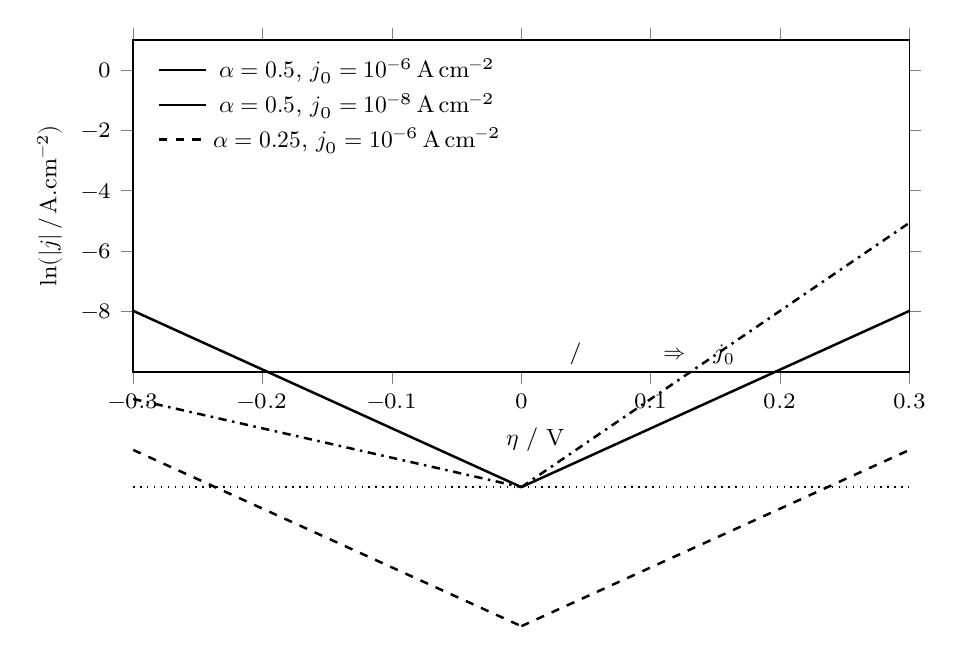
\begin{tikzpicture}
\begin{axis}[
  width=\dimexpr\twocolwidth-2mm\relax, height=58mm,
  xlabel={过电位 $\eta$ / V}, ylabel={$\ln(|j|\,/\,\mathrm{A.cm^{-2}})$},
  xmin=-0.30, xmax=0.30, ymin=-10, ymax=1,
  xtick={-0.3,-0.2,-0.1,0,0.1,0.2,0.3},
  ytick={-8,-6,-4,-2,0},
  legend style={at={(0.02,0.98)},anchor=north west,legend columns=1},
  clip=false
]
% alpha = 0.5, f = F/RT ≈ 38.92 V^-1 at 298 K ; log10 scale factor ln -> use natural log
% ln|j| = ln j0 - alpha*f*eta   (cathodic, eta<0 gives increase), anodic mirrored
\addplot[mainline,black,domain=-0.30:0,samples=80]{ln(1e-6) - 0.5*38.92*x};
\addplot[mainline,black,domain=0:0.30,samples=80]{ln(1e-6) + 0.5*38.92*x};
\addlegendentry{$\alpha=0.5$, $j_0=\qty{e-6}{\A\per\square\cm}$}
\addplot[mainline,black,dashed,domain=-0.30:0,samples=80]{ln(1e-8) - 0.5*38.92*x};
\addplot[mainline,black,dashed,domain=0:0.30,samples=80]{ln(1e-8) + 0.5*38.92*x};
\addlegendentry{$\alpha=0.5$, $j_0=\qty{e-8}{\A\per\square\cm}$}
\addplot[mainline,black,dashdotted,domain=-0.30:0,samples=80]{ln(1e-6) - 0.25*38.92*x};
\addplot[mainline,black,dashdotted,domain=0:0.30,samples=80]{ln(1e-6) + 0.75*38.92*x};
\addlegendentry{$\alpha=0.25$, $j_0=\qty{e-6}{\A\per\square\cm}$}
\addplot[thinline,black,dotted,domain=-0.30:0.30,samples=2]{ln(1e-6)};
\node[anchor=west,font={\fontsize{8}{9.5}\selectfont}] at (axis cs:0.02,-9.4)
  {实线/虚线：斜率相同、截距不同 $\Rightarrow$ 只差 $j_0$};
\end{axis}
\end{tikzpicture}
\caption{Butler--Volmer 方程在高过电位极限下的 Tafel 图（模型计算，$\qty{298}{K}$）。
读者应看两件事：\textbf{同一斜率、不同截距}只反映 $j_0$ 的差别（实线对虚线，差两个
数量级）；\textbf{斜率改变}反映传递系数 $\alpha$ 的差别（点划线，阴极支 $\alpha=0.25$，
$\alpha$ 越小斜率越陡）。值得注意的局限：真实体系的 Tafel 图常在中段出现折点，
说明速率控制步骤随过电位切换，此时用一条直线拟合全区间会同时给出错误的 $\alpha$ 与
$j_0$；低过电位区（$|\eta|<\qty{50}{mV}$）应改用 \equref{eq:bv-linear} 的线性关系。
\modelmark}
\label{fig:tafel}
\end{figure}

\subsubsection{静态电极过程中的物质传递影响}

前面所有含有电极表面浓度 $C_{\mathrm{O}}$ 的式子都留了一个未定的量。除平衡态等特殊
情形外，本体浓度 $C^*$ 与表面浓度 $C$ 并不相等，因此\textbf{表面浓度信息是理解浓差
极化行为的关键}。溶液中物质传递有迁移、扩散、对流三种形式；对\textbf{静态电极}，
对流可忽略；若溶液中有\textbf{过量支持电解质}，电迁移也可不考虑。此时电极周围传质由
扩散控制，符合 Fick 扩散定律，速率与浓度梯度成正比：

\begin{equation}
N_{\mathrm{O}}=-D_{\mathrm{O}}\left(\frac{\partial C_{\mathrm{O}}}{\partial x}\right)
\label{eq:fick1}
\end{equation}

\src{式 11-31，书内 p.818 / PDF p.306}。式中 $N_{\mathrm{O}}$ 为距电极表面 $x$ 处物质
$\mathrm{O}$ 的流量（$\mathrm{mol.s^{-1}.cm^{-2}}$），$D_{\mathrm{O}}$ 为扩散系数
（$\mathrm{cm^2.s^{-1}}$）。\textbf{符号约定（本节与式~\eqref{eq:current-basic} 统一）}：
坐标 $x$ 由电极表面指向溶液本体，$N_{\mathrm{O}}$ 为沿 $+x$ 方向的流量；电流取
\textbf{「还原为正」}，即 $i=i_{\mathrm{f}}-i_{\mathrm{b}}$，故
$i=-nFA\,N_{\mathrm{O}}|_{x\to0}$——还原时物质向 $-x$（朝电极）输运，$N_{\mathrm{O}}<0$，
电流为正。

\paragraph{Nernst 扩散层与极限电流} 假设电极表面存在厚度为 $\delta_{\mathrm{O}}$ 的
静止层，$x=\delta_{\mathrm{O}}$ 以外浓度均为本体浓度 $C_{\mathrm{O}}^*$，传递到电极表面
的物质被完全消耗。静止层内浓度线性上升，
$\partial C_{\mathrm{O}}/\partial x\approx
(C_{\mathrm{O}}^*-C_{\mathrm{O}})/\delta_{\mathrm{O}}>0$，由式~\eqref{eq:fick1} 与上述
$i=-nFA\,N_{\mathrm{O}}$（Faraday 定律）得

\begin{equation}
\frac{i}{nFA}=D_{\mathrm{O}}
\frac{C_{\mathrm{O}}^*-C_{\mathrm{O}}}{\delta_{\mathrm{O}}}
\label{eq:diff-layer}
\end{equation}

当表面浓度 $C_{\mathrm{O}}=0$ 时传递速率达到最大，电流达到平台值，称为\textbf{极限电流}
$i_{\mathrm{t}}$：

\begin{equation}
\frac{i_{\mathrm{t}}}{nFA}=D_{\mathrm{O}}
\frac{C_{\mathrm{O}}^*}{\delta_{\mathrm{O}}}
\label{eq:il}
\end{equation}

\src{式 11-32、11-33，书内 p.819 / PDF p.307}。还原时 $C_{\mathrm{O}}^*>C_{\mathrm{O}}$，
故 $i>0$、$i_{\mathrm{t}}>0$，与动力学式~\eqref{eq:current-basic}（$i_{\mathrm{f}}>0$ 为
还原）以及后面的 Cottrell 式~\eqref{eq:cottrell} 同号，同时也与
\equref{eq:tafel} 成立条件中的 $i\ll i_{\mathrm{t}}$ 自洽。若讨论的是反向的氧化过程，
把浓度差换成 $C_{\mathrm{R}}-C_{\mathrm{R}}^*$，电流随之变号。$i_{\mathrm{t}}$ 只表征
电极表面的传质情况，\textbf{不含任何动力学信息}——这一点在后面每一种方法里都会再出现。
量纲检查：$[nFAD C^*/\delta]=(\mathrm{C.mol^{-1}})\mathrm{cm^2}
(\mathrm{cm^2.s^{-1}})(\mathrm{mol.cm^{-3}})/\mathrm{cm}=\mathrm{C.s^{-1}}=\mathrm{A}$。
\tocheck{未对照原页面图像：原书式（11-32）（11-33）写作
$i/nFA=-D_{\mathrm{O}}(C_{\mathrm{O}}^*-C_{\mathrm{O}})/\delta_{\mathrm{O}}$
（OCR 中负号可辨），即扩散部分取「还原为负」的取向，与式（11-16）的「还原为正」
相反；本稿统一为还原为正，并写明 $x$ 的取向与 $i=-nFA N_{\mathrm{O}}$。其后式
（11-36）—（11-40）只含比值 $i_{\mathrm{t}}/(i_{\mathrm{t}}-i)$，在两套取向下的数值完全
相同，故未改动；原页面图像未对照。}

\paragraph{浓差过电位的分解} 表面浓度对电极电势的影响可拆成热力学与动力学两部分。
由 Nernst 方程，本体浓度与表面浓度对应的电势差为
$\eta_1=\dfrac{RT}{nF}\ln\dfrac{C_{\mathrm{O}}}{C_{\mathrm{O}}^*}$
\src{式 11-34、11-35，书内 p.819 / PDF p.307}；把 \equref{eq:diff-layer} 与
\equref{eq:il} 代入，得

\begin{equation}
\eta_1=-\frac{RT}{nF}\ln\!\left(\frac{i_{\mathrm{t}}}{i_{\mathrm{t}}-i}\right)
\label{eq:eta1}
\end{equation}

再按 Butler--Volmer 方程在高电流密度区略去第二项，得到
$i=i_0\dfrac{C_{\mathrm{O}}}{C_{\mathrm{O}}^*}
\exp\!\left(-\dfrac{\alpha nF\eta}{RT}\right)$ 及其重排
$\eta=-\dfrac{RT}{\alpha nF}\left(\ln\dfrac{i}{i_0}
+\ln\dfrac{C_{\mathrm{O}}^*}{C_{\mathrm{O}}}\right)$
\src{式 11-37、11-38，书内 p.819 / PDF p.307}。只保留浓度项即

\begin{equation}
\eta_2=-\frac{RT}{\alpha nF}\ln\frac{C_{\mathrm{O}}^*}{C_{\mathrm{O}}}
=-\frac{RT}{\alpha nF}\ln\!\left(\frac{i_{\mathrm{t}}}{i_{\mathrm{t}}-i}\right)
\label{eq:eta2}
\end{equation}

两部分之和给出电极表面浓度造成的总电势损失：

\begin{equation}
\eta_{\mathrm{conc}}=\eta_1+\eta_2
=-\frac{RT}{nF}\left(1+\frac{1}{\alpha}\right)
\ln\!\left(\frac{i_{\mathrm{t}}}{i_{\mathrm{t}}-i}\right)
\label{eq:eta-conc}
\end{equation}

\begin{keycond}
\equref{eq:eta1}—\equref{eq:eta-conc} 的成立条件是\textbf{静态电极 + 过量支持电解质 +
Nernst 扩散层模型 + 高过电位下略去 Butler--Volmer 的阳极项}。量纲检查：
$[RT/(\alpha nF)]=\mathrm{V}$，$[\ln(\cdot)]$ 无量纲，成立。两个极限行为要记牢：
$i\to 0$ 时 $\eta_{\mathrm{conc}}\to 0$（传质不构成限制）；$i\to i_{\mathrm{t}}$ 时
$\eta_{\mathrm{conc}}\to\infty$（浓差极化发散，电流被钉在平台值上）。
\tocheck{未对照原页面图像：书中式（11-40）OCR 为
$\eta_{\mathrm{conc}}=\eta_1+\eta_2=-\frac{RT}{nF}(1+\frac{1}{\alpha})(\frac{i_{\mathrm{t}}}{i_{\mathrm{t}}-i})$，
疑漏对数号（否则量纲为 V 而右端无量纲），本分片按 \equref{eq:eta1}、\equref{eq:eta2}
的标准形式补回 $\ln$，系数 $(1+1/\alpha)$ 沿用原书。}
\end{keycond}

图~\ref{fig:series} 把本节与上一节的关系画成一张图：电荷转移与传质是\textbf{串联}的
两步，二者共用同一个电流，因此\textbf{总速率由较慢的一步决定}。

\begin{figure}[htbp]
\centering
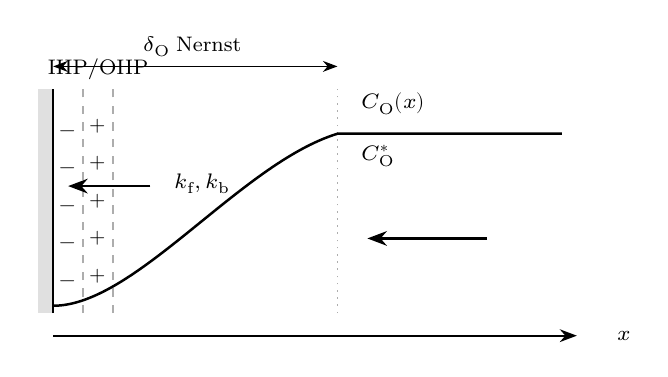
\begin{tikzpicture}[x=1mm,y=1mm,>=Stealth,scale=0.95,transform shape]% width=\onecolwidth
% --- electrode (left) ---
\fill[black!12] (-2,0) rectangle (0,30);
\draw[axisline] (0,0) -- (0,30);
\node[rotate=90,anchor=south,font={\fontsize{8}{9.5}\selectfont}] at (-1.0,15) {电极（电子导体）};
% --- x axis ---
\draw[axisline,->] (0,-3) -- (70,-3) node[anchor=west,font={\fontsize{8}{9.5}\selectfont}]{本体溶液 $x$};
% --- IHP/OHP ---
\draw[accentsoft,dashed,line width=0.6pt] (4,0) -- (4,30);
\draw[accentsoft,dashed,line width=0.6pt] (8,0) -- (8,30);
\node[anchor=south,font={\fontsize{8}{9.5}\selectfont}] at (6,30) {IHP/OHP};
% --- double layer charges ---
\foreach \y in {4,9,14,19,24}{\node[font={\fontsize{8}{9.5}\selectfont}] at (2,\y) {$-$};}
\foreach \y in {5,10,15,20,25}{\node[font={\fontsize{8}{9.5}\selectfont}] at (6,\y) {$+$};}
% --- diffusion layer span ---
\draw[<->,thinline] (0,33) -- (38,33)
  node[midway,above,font={\fontsize{8}{9.5}\selectfont}]{扩散层 $\delta_{\mathrm{O}}$（Nernst 静止层）};
\draw[accentsoft,dotted,line width=0.6pt] (38,0) -- (38,30);
% --- concentration profile ---
\draw[mainline] (0,1) .. controls (11,1) and (25,20) .. (38,24) -- (68,24);
\node[anchor=west,font={\fontsize{8}{9.5}\selectfont}] at (40,28) {$C_{\mathrm{O}}(x)$};
\node[anchor=west,font={\fontsize{8}{9.5}\selectfont}] at (40,21) {$C_{\mathrm{O}}^*$（本体浓度）};
% --- arrows ---
\draw[->,mainline] (58,10) -- (42,10);
\node[anchor=west,font={\fontsize{8}{9.5}\selectfont}] at (59,10) {扩散};
\draw[->,mainline] (13,17) -- (2,17);
\node[anchor=west,font={\fontsize{8}{9.5}\selectfont},text width=26mm] at (15,18)
  {电荷转移\\ $k_{\mathrm{f}},k_{\mathrm{b}}$};
\end{tikzpicture}
\caption{静态电极界面的双电层与扩散层示意，以及传质与电荷转移的串联位置（示意）。
读者应看三处：紧贴电极的 \textbf{IHP/OHP} 与电荷符号代表双电层，其充放电构成
\textbf{非法拉第电流}；向右延伸的 $\delta_{\mathrm{O}}$ 是\textbf{扩散层}，其中的浓度
梯度决定传质速率；电流必须依次通过这两步，故总速率由较慢者决定。局限：本图为
Nernst 静止层的简化图像，真实扩散层没有明确边界，仅在无对流且有支持电解质时近似
成立；双电层被简化为单层符号，未画出溶剂化与特性吸附。\schemamark\figsrc{据 S2
（下册）§11.1.5 与图 11-2 改绘；书内 p.817—819，PDF p.305—307。}}
\label{fig:series}
\end{figure}

\begin{crosscheck}
\textbf{怎么判断自己测的是传质还是电荷转移？} 三个互不依赖的检验：（i）
\emph{改变传质速率}——提高搅拌或旋转速率，若电流随之增大，说明传质仍在限制；
（ii）\emph{改变浓度}——若电流正比于 $C^*$（扩散控制）而不随催化剂本征性质变化，
说明读到的是极限电流；（iii）\emph{改变电极面积}——真实面积加倍而电流不成比例增加，
说明电流被溶液侧传质「钉住」。三条中只要有一条指向传质，就不能把该电流当作本征活性。
与流体动力学方法（11.3 起）的 Levich 关系互为回查：若 $j^{-1}$ 对 $\omega^{-1/2}$ 作图
得直线，其截距才对应本征动力学。
\end{crosscheck}

\subsection{控制电势的研究方法}

\subsubsection{实验装置与共同假定}

本节的方法都靠\textbf{已知的程序强制电极电势按预定函数变化}，同时测定电流随时间或
电势变化的特征曲线\src{S2 §11.2，书内 p.819 / PDF p.307}。装置包含函数发生器、恒电势仪
（potentiostat）与电解池：函数发生器设定电势程序，恒电势仪通过高阻抗反馈回路测量工作
电极与参比电极间的电势差，并\textbf{随时注入电流}以保证该电势差与程序一致
\src{图 11-3，书内 p.820 / PDF p.308}。对电极承担全部电流，参比电极因接在高阻抗回路上
而基本不取电流——这是「测量不扰动体系」的前提。

\begin{keycond}
本节所有方法都假定\textbf{面积体积比 $A/V$ 很小}，以保证测试过程中电活性物质的
\emph{本体}浓度不因电解而显著变化。实现方式是选用\textbf{微电极}（microelectrode）
并在足够大体积的溶液中做短时间实验。若违反此假定，$C^*$ 会随实验进程下降，
所有基于恒定 $C^*$ 的方程（Cottrell、Levich、Tafel 截距）都会随时间漂移，
表现为「同一电极重复扫描，峰高逐圈下降」。
\end{keycond}

\begin{measure}
\textbf{报告任何一条电势--电流曲线之前，这五项必须实测并记录。}
\textbf{（1）参比电极}：种类、内充液浓度、\qty{25}{\celsius} 下的标定值、实验前后漂移
（用饱和 \ce{KCl} 或标准缓冲液标定，漂移超过约 \qty{1}{mV} 的数据应作废）；
\textbf{（2）温度}：溶液温度及其稳定性，因为 $RT/F$ 直接进入所有斜率与截距；
\textbf{（3）未补偿电阻 $R_{\mathrm{u}}$}：由高频阻抗外推或电流中断法测出，记录
\textbf{补偿比例}（如 85\% 补偿）与残余 $iR_{\mathrm{u}}$ 降；\textbf{（4）双电层电容
$C_{\mathrm{d}}$ 与时间常数 $\tau=R_{\mathrm{u}}C_{\mathrm{d}}$}：决定哪些时间窗的数据
可用；\textbf{（5）面积基准}：几何面积 $A_{\mathrm{g}}$ 与真实面积 $A_{\mathrm{m}}$ 及其
定标方法（氢吸附电量或 $C_{\mathrm{d}}$）。这五项缺任何一项，Tafel 斜率与 $j_0$ 都
不可与文献直接比较。
\end{measure}

\subsubsection{电势阶跃法}

\paragraph{计时电流法} 给体系一个电势阶跃，测定电流随时间的变化
（chronoamperometry）\src{图 11-4，书内 p.820 / PDF p.308}。典型设置是：反应物
$\mathrm{O}$ 在初始电势 $E_1$ 不反应，阶跃到 $E_2$ 后以扩散极限速度被还原。
相关的两类变体用于获得更多信息：

\begin{itemize}
\item \textbf{取样电流伏安法}（sampled-current voltammetry）：做一系列电势阶跃，
  在初始条件相同的前提下分别测 $i$--$t$ 曲线，再用阶跃后某一固定时刻的电流对阶跃
  电势作图，得到「伏安图」\src{图 11-5，书内 p.821 / PDF p.309}。
\item \textbf{双电势阶跃计时电流法}（double potential step chronoamperometry）：
  先阶跃再跃回初始值，是反向技术，用于研究较复杂的电极反应，特别是中间产物的去向
  \src{图 11-6，书内 p.821 / PDF p.309}。
\end{itemize}

记录电流对时间的\textbf{积分}即通过的电量，相应方法统称库仑方法，最基本的是计时库仑法
与双电势阶跃计时库仑法，它们就是上述计时电流法的积分量
\src{图 11-7，书内 p.822 / PDF p.310}。

\paragraph{扩散控制的电势阶跃：Cottrell 方程} 指瞬间施加一个大电势阶跃，使电极表面
物质浓度为零；此后继续加大电势不再改变 $i$--$t$ 曲线，电流主要受溶液传质速率控制。
对平板电极，解线性扩散方程（Fick 第二定律）

\begin{equation}
\frac{\partial C_{\mathrm{O}}(x,t)}{\partial t}
=D_{\mathrm{O}}\frac{\partial^2 C_{\mathrm{O}}(x,t)}{\partial x^2}
\label{eq:fick2}
\end{equation}

边界条件为：初始 $C_{\mathrm{O}}(x,0)=C_{\mathrm{O}}^*$；
$\lim_{x\to\infty}C_{\mathrm{O}}(x,t)=C_{\mathrm{O}}^*$；阶跃后表面
$C_{\mathrm{O}}(0,t)=0\ (t>0)$ \src{式 11-41—11-44，书内 p.822 / PDF p.310}。解得
\textbf{Cottrell 方程}

\begin{equation}
i(t)=i_{\mathrm{d}}(t)=\frac{nFAD_{\mathrm{O}}^{1/2}C_{\mathrm{O}}^*}{(\pi t)^{1/2}}
\label{eq:cottrell}
\end{equation}

\src{式 11-45，书内 p.822 / PDF p.310}。表面附近电活性物质的贫化效应造成电流与
$t^{1/2}$ 呈\textbf{倒数}关系，这正是电解速度受扩散控制的标志。

\begin{keycond}
\eqref{eq:cottrell} 的成立条件：\textbf{（i）平板电极、半无限线性扩散}；
\textbf{（ii）阶跃足够大，使表面浓度瞬间降为零（极限扩散）}；\textbf{（iii）无对流、
有惰性支持电解质（电迁移被抑制）}；\textbf{（iv）$C^*$ 在实验期间不变（$A/V$ 小）}。
量纲检查：$[nFAD^{1/2}C^*/(\pi t)^{1/2}]
=(\mathrm{C.mol^{-1}})(\mathrm{cm^2})(\mathrm{cm.s^{-1/2}})(\mathrm{mol.cm^{-3}})
/(\mathrm{s^{1/2}})=\mathrm{C.s^{-1}}=\mathrm{A}$，成立。
\textbf{实操上必须扣除两个非理想项}：电流起始段受恒电势仪输出能力限制；阶跃瞬间还有
非法拉第的\textbf{双电层充电电流}，它按电解池时间常数 $\tau=R_{\mathrm{u}}C_{\mathrm{d}}$
（$R_{\mathrm{u}}$ 为未补偿电阻，$C_{\mathrm{d}}$ 为双电层电容）指数衰减，即使经过
$5\tau$ 后对总电流仍有可观贡献，从中很难精确分离法拉第电流。此外长时间实验中浓度梯度
与振动会造成对流扰动，表现为\textbf{电流大于} Cottrell 计算值。
\end{keycond}

相应的浓度分布为

\begin{equation}
C_{\mathrm{O}}(x,t)=C_{\mathrm{O}}^*\left[1-\mathrm{erfc}
\left(\frac{x}{2(D_{\mathrm{O}}t)^{1/2}}\right)\right]
=C_{\mathrm{O}}^*\,\mathrm{erf}\!\left(\frac{x}{2(D_{\mathrm{O}}t)^{1/2}}\right)
\label{eq:conc-profile}
\end{equation}

\src{式 11-46、11-47，书内 p.823 / PDF p.311}。不同时刻的浓度分布显示电极附近的氧化态
被耗尽，且\textbf{表面浓度梯度随时间变小}——这正是电流随时间衰减的几何原因。

\paragraph{球形扩散与超微电极} 对球形扩散（如悬汞电极）需用球坐标下的扩散方程

\begin{equation}
\frac{\partial C_{\mathrm{O}}(r,t)}{\partial t}
=D_{\mathrm{O}}\left[\frac{\partial^2 C_{\mathrm{O}}(r,t)}{\partial r^2}
+\frac{2}{r}\frac{\partial C_{\mathrm{O}}(r,t)}{\partial r}\right]
\label{eq:fick2-sph}
\end{equation}

$r$ 为距球心的径向距离，电极半径 $r_0$，边界条件为
$C_{\mathrm{O}}(r,0)=C_{\mathrm{O}}^*(r>r_0)$、
$\lim_{r\to\infty}C_{\mathrm{O}}(r,t)=C_{\mathrm{O}}^*$、
$C_{\mathrm{O}}(r_0,t)=0\,(t>0)$ \src{式 11-48—11-51，书内 p.824 / PDF p.312}。解得

\begin{equation}
i_{\mathrm{d}}(t)=nFAD_{\mathrm{O}}C_{\mathrm{O}}^*
\left[\frac{1}{(\pi D_{\mathrm{O}}t)^{1/2}}+\frac{1}{r_0}\right]
=i_{\mathrm{d}}(\text{线性})+\frac{nFAD_{\mathrm{O}}C_{\mathrm{O}}^*}{r_0}
\label{eq:spherical}
\end{equation}

\src{式 11-52、11-53，书内 p.824 / PDF p.312}。量纲检查：第二项
$[nFADC^*/r_0]=(\mathrm{C.mol^{-1}})(\mathrm{cm^2})(\mathrm{cm^2.s^{-1}})
(\mathrm{mol.cm^{-3}})/\mathrm{cm}=\mathrm{A}$，与第一项同量纲。
关键结论是：\textbf{球形扩散多出一个与时间无关的项}，这使电流在长时间区趋向稳态，
而不是像平板电极那样衰减到零。浓度分布的形式与线性情形非常相似，只差一个
$r_0/r$ 系数；若扩散层远薄于电极半径，球形电极的行为与平面电极无异。

\paragraph{粗糙度与超微电极} 实际电极表面总不像理想条件那样平滑洁净，故引入粗糙度
$\rho=A_{\mathrm{m}}/A_{\mathrm{g}}$：$A_{\mathrm{m}}$ 为微观（真实）面积，可由测双电层
电容或测电极表面形成单分子层所需电量来测定；$A_{\mathrm{g}}$ 为几何面积，即电极表面
正投影所得的面积 \src{书内 p.824 / PDF p.312}。\textbf{所有电流密度都必须说明用的是
哪个面积。} 超微电极因尺寸小而使实验结果与理论计算相近，故被广泛使用；本书界定其
临界尺寸小于 \qty{10}{nm}。短时间区扩散层厚度小于临界尺寸，可用 Cottrell 方程
（半无限线性扩散）计算电流；长时间区扩散层厚度较大，电流趋于稳态或准稳态

\begin{equation}
i_{\mathrm{ss}}=nFAm_0C_{\mathrm{O}}^*
\label{eq:iss-ch11}
\end{equation}

\src{式 11-55，书内 p.825 / PDF p.313}。\tocheck{未对照原页面图像：式中 $m_0$ 在原书
未在前文定义，按上下文应为传质系数（$\mathrm{cm.s^{-1}}$），其与 $D_{\mathrm{O}}$ 及
电极几何的关系（半球形 $m_0=2D/r_0$、球形 $4D/r_0$、嵌盘 $4D/(\pi r_0)$ 等）书中未给，
本分片不代为指定。}

\paragraph{取样电流伏安法的响应与信息边界} 对可逆电极反应，平板电极（满足半无限线性
扩散）对\textbf{任意}单电势阶跃的电流响应为

\begin{equation}
i(t)=\frac{nFAD_{\mathrm{O}}^{1/2}C_{\mathrm{O}}^*}
{\pi^{1/2}t^{1/2}\,(1+\theta)}
\label{eq:sampled-rev}
\end{equation}

它是可逆体系对电势阶跃的一般响应式，极限扩散（$\theta\to0$）时即还原为 Cottrell 方程
\src{式 11-56，书内 p.825 / PDF p.313}。此外，\textbf{电极形状并不是关键}，只要满足
「扩散层厚度小于电极曲率半径」即可。超微球形电极上述模型的稳态区响应为
$i=\dfrac{nFAD_{\mathrm{O}}C_{\mathrm{O}}^*}{(1+\xi_2\theta)r_0}$
\src{式 11-57，书内 p.825 / PDF p.313}。
\tocheck{未对照原页面图像：式（11-56）（11-57）中的符号 $\theta$、$\xi_2$ 在原书未在
本分片可见范围内定义，OCR 亦可能把 $\theta$/$\vartheta$ 或下标记错。本分片保留原符号
并只使用其定性结论（$\theta\to0$ 退化为 Cottrell），未据此做数值计算。}

可逆体系下取样电流伏安法能给出与不能给出的信息很不相同：

\begin{itemize}
\item \textbf{能}：由波高测浓度，用于校正或测量标准添加物的浓度；可逆波的形状与位置
  反映电极反应的能量依赖性，由此可得\textbf{标准电势、自由能、平衡常数}；半波电势接近
  形式电势，故可用于估算尚未定性的化学体系的电势。
\item \textbf{不能}：\textbf{不能得到动力学信息}。可逆波只报告热力学，因为传质已经完全
  接管了电流的大小。
\end{itemize}

对准可逆与不可逆反应，平板电极的响应形如
$i=FA\left(k_{\mathrm{f}}C_{\mathrm{O}}^*-k_{\mathrm{b}}C_{\mathrm{R}}^*\right)
\exp(H^2t)\,\mathrm{erfc}(Ht^{1/2})$，球形电极的稳态响应另含
$D_{\mathrm{O}}$、$r_0$ 与速率常数之比 \src{式 11-58、11-59，书内 p.825 / PDF p.313}。
\tocheck{未对照原页面图像：式（11-58）中 $H$ 的定义、式（11-59）中括号内的
$(\delta+1)$ 结构均无法从 OCR 复原，本分片只用其定性形式与下述结论，未代入数值。}
其信息边界为：准可逆与不可逆波的\textbf{极限电流平台仍完全受扩散控制}，故仍可用于求
$C^*$、$n$、$A$、$D$、$r_0$ 等任何对 $i_{\mathrm{d}}$ 有贡献的参数；准可逆波有时可
给出形式电势的近似值，而不可逆波因半波电势偏离形式电势\textbf{无法求得热力学信息}；
但完全不可逆波的波形与位置可以提供\textbf{动力学}信息。

\paragraph{计时电量法} 计时电量法记录电量与时间的关系 $Q(t)$，常用于代替计时电流法，
有三个优势：信号随时间增长，暂态后期受阶跃瞬间非理想电势变化的影响较轻微，信噪比好；
暂态电流中的随机噪声因积分而平滑；\textbf{可以区分双电层充电、吸附物质的电极反应与
扩散反应物法拉第反应对电量的贡献}，因而便于研究表面过程。对 Cottrell 公式积分得

\begin{equation}
Q_{\mathrm{d}}=\frac{2nFAD_{\mathrm{O}}^{1/2}C_{\mathrm{O}}^*t^{1/2}}{\pi^{1/2}}
\label{eq:chronocoul}
\end{equation}

但实际电量还含双电层充电与还原吸附的某种氧化态所贡献的部分，$Q$ 对 $t^{1/2}$ 的直线
一般不通过原点。这些电量只在瞬间出现、不随时间累积，故作为两个与时间无关的附加项写出：

\begin{equation}
Q=\frac{2nFAD_{\mathrm{O}}^{1/2}C_{\mathrm{O}}^*t^{1/2}}{\pi^{1/2}}
+Q_{\mathrm{dl}}+nFA\Gamma_{\mathrm{O}}
\label{eq:chronocoul-full}
\end{equation}

式中 $Q_{\mathrm{dl}}$ 为电容电量，$nFA\Gamma_{\mathrm{O}}$ 为表面吸附的
$\mathrm{O}$ 还原的法拉第分量 \src{式 11-60、11-61，书内 p.826 / PDF p.314}。
量纲检查：$[nFAD^{1/2}C^*t^{1/2}/\pi^{1/2}]=(\mathrm{C.mol^{-1}})(\mathrm{cm^2})
(\mathrm{cm.s^{-1/2}})(\mathrm{mol.cm^{-3}})(\mathrm{s^{1/2}})=\mathrm{C}$，成立；
$[nFA\Gamma]=\mathrm{C.mol^{-1}}\cdot\mathrm{cm^2}\cdot\mathrm{mol.cm^{-2}}=\mathrm{C}$，
同量纲。\textbf{这条式子的实践价值在于把「非法拉第背景」变成了可读出的截距}：
用不同电势阶跃做 $Q$--$t^{1/2}$ 图，截距对电势作图为直线，斜率即 $C_{\mathrm{d}}$，
由此可测真实面积；剩余截距来自吸附物种。这一方法常用于测定电活性物质的表面余量，
但需要再做反向实验。

\begin{dataflow}
\textbf{从一条 $i$--$t$ 曲线到结论，只能走这五步。} （1）确认阶跃电势足够大，
表面浓度确实为零（否则 \equref{eq:cottrell} 不适用）。（2）判断时间窗：
$t<5\tau$（$\tau=R_{\mathrm{u}}C_{\mathrm{d}}$）的数据必须丢弃，双电层充电尚未衰减；
长时间区要检查 $i\,t^{1/2}$ 是否仍为常数。（3）作 $i$--$t^{-1/2}$ 图，直线斜率给出
$nFAD^{1/2}C^*/\pi^{1/2}$；斜率过原点才说明纯扩散控制。（4）由斜率反解 $D$ 或 $C^*$
时，必须固定另一个量；用\emph{同一个}面积定义（$A_{\mathrm{m}}$ 或 $A_{\mathrm{g}}$）。
（5）只有在确认 $i$--$t^{-1/2}$ 直线的截距为零之后，才能说「本体系在此时标下是纯扩散
控制」；截距非零通常意味着还有电荷转移阻力或吸附贡献。需要本征动力学时，改做取样电流
伏安法并处理 \equref{eq:sampled-rev} 形式的响应。
\end{dataflow}

\subsubsection{电势扫描法}

电势扫描法随时间扫描电势并记录电流--电势曲线，以获得体系完整的电化学行为。主要分为
\textbf{线性扫描伏安法}（linear sweep voltammetry，LSV）与\textbf{循环伏安法}
（cyclic voltammetry，CV）\src{S2 §11.2.2、图 11-9，书内 p.826—827 / PDF p.314—315}。

\paragraph{从一条 CV 读出什么：\ce{Pt} 单晶在 \ce{H2SO4} 中的例子} 以 \ce{Pt} 在
\qty{0.5}{mol.L^{-1}} \ce{H2SO4} 中的 CV（\qty{50}{mV.s^{-1}}）为例
\src{图 11-10，书内 p.827 / PDF p.315}。测量前先把单晶表面在氢氧火焰中退火：一是完全
除去表面吸附的杂质，二是使原子完全按规则排列。退火过程中 \ce{Pt} 表面会吸附氧形成氧
吸附层。扫描从\textbf{开路电势 OCP} 出发往低电势方向进行。

读图顺序与每个峰的归属：先出现的峰来自表面已吸附的氧随电势降低被电还原；第二个过程是
溶液中 \ce{H+} 得电子还原为氢原子并吸附在 \ce{Pt} 表面，而正向扫描时对应的是吸附氢的
电氧化，即该反应的逆反应。其他单晶上这些氧峰与氢峰同样存在，但\textbf{峰的形状和位置
不同}，因为表面 \ce{Pt} 原子的排列方式不同——因此峰形特征可用来辨别晶面是 (100)、
(110) 还是 (111)。

\paragraph{氢吸附电量与真实面积} 对氢吸附峰积分，所得面积即为氢吸附产生的电量
（电流$\times$时间 = 电量）。由电量可算出吸附氢原子的数目；不同晶面 $Q_{\mathrm{H}}$
不同。再由晶面上原子的排列方式与原子直径可算出单位面积的 \ce{Pt} 原子数，两者比较
发现数值很接近，说明\textbf{一个 \ce{Pt} 原子吸附一个 H}。由于电活性物质（H 和 O）反复
氧化还原吸脱附，表面会逐渐粗糙，单晶表面最终变成多晶表面；多晶表面由若干小单晶面
组成，反映的是这些单晶的平均行为 \src{图 11-11，书内 p.828 / PDF p.316}。

多晶 \ce{Pt}（\ce{Pt} 丝、纳米 \ce{Pt} 黑）的 CV 分三个区域：左侧峰对应氢的吸附与脱附，
不同峰来自氢在不同晶面上的吸附；右侧峰是氧的吸附与脱附，即 \ce{Pt} 表面的氧化与还原，
不同峰代表不同氧化态（可能有 \ce{Pt-OH}、\ce{PtO_x} 等，更详细的归属仍未知）；中间区域
是\textbf{双电层区}，该区电流由双电层充放电引起、没有氧化还原反应。对该区积分可求得
双电层电量。由于一个 \ce{Pt} 原子只吸附一个氢原子，\textbf{$Q_{\mathrm{H}}/Q$ 即 \ce{Pt}
的真实表面积}——这就是用 H 的吸脱附测定 \ce{Pt} 真实表面积的方法
\src{书内 p.829 / PDF p.317}。

\begin{dataflow}
\textbf{为什么必须用真实面积。} 实验能测的是整个电极面积上产生的电流，面积越大电流
越大。因此\textbf{忽略电极面积、直接用电流大小表示反应速率的快慢，既不科学也不准确}。
规范做法是用\textbf{电流密度}（单位电极面积上的电流）表示反应速率，而这个面积必须是
\textbf{真实（电化学活性）面积}，即由氢吸附电量 $Q_{\mathrm{H}}$ 或双电层电容定标得到的
面积，而不是电极的几何尺寸。报告数据时必须同时给出：面积基准、定标方法、以及
$\rho=A_{\mathrm{m}}/A_{\mathrm{g}}$ 的数值或范围。
\end{dataflow}

\paragraph{可逆性判据} 由 CV 的形状可以判断电极反应属于可逆、准可逆还是不可逆，其判据
与「能得到什么信息」直接对应：

\begin{keycond}
\textbf{可逆（Nernst 型）}：峰电流 $i_{\mathrm{p}}$ 正比于 $v^{1/2}$；峰电位差
$\Delta E_{\mathrm{p}}=|E_{\mathrm{pa}}-E_{\mathrm{pc}}|\approx 2.303RT/(nF)$，即
\qty{25}{\celsius} 下约 $59/n$ mV，且\textbf{不随扫描速率变化}；$i_{\mathrm{pa}}/i_{\mathrm{pc}}
\approx1$；$E_{\mathrm{p}}$ 与 $v$ 无关。\textbf{准可逆}：$\Delta E_{\mathrm{p}}$ 随 $v$
增大而增大，峰仍然成对。\textbf{不可逆}：只出现单向峰，$E_{\mathrm{p}}$ 随 $v$ 增大而
向更负（阴极）或更正（阳极）方向移动，约每十倍 $v$ 移动 $30/(\alpha n)$ mV。
\textbf{判据的成立条件是反应物与产物都溶于溶液且无后续化学反应}；若产物发生吸附或
偶联化学反应，$i_{\mathrm{pa}}/i_{\mathrm{pc}}$ 会显著偏离 1，此时不能直接判为不可逆。
\tocheck{未对照原页面图像：分片 a 的源文本（图 11-9、11-10 说明）未展开 CV 的定量判据
公式，本节判据按电化学标准形式重建；若本书 11.2.2 后有专门的判据小节，应由后一分片
或统一核验时对齐符号（是否用 $D^{1/2}$、是否含 $n^{3/2}$、是否讨论 $\Delta E_{\mathrm{p}}$
的严格表值）。}
\end{keycond}

\begin{pitfall}
\textbf{控制电势实验的五类系统性误判，按出现频率排序。}
\textbf{（1）未做 iR 补偿导致 Tafel 斜率失真。} 实测电势含 $iR_{\mathrm{u}}$ 降：
$E_{\text{实测}}=E_{\text{真}}+iR_{\mathrm{u}}$，故按 $\eta$--$\lg i$ 作图得到的表观斜率
为 $b_{\text{表观}}=b+2.303R_{\mathrm{u}}A$（以电流作图时）或 $b+2.303R_{\mathrm{u}}j$
（以电流密度作图时）。这意味着\textbf{高电流段被系统性抬高}，Tafel 图向上弯折、斜率变大；
电流越大失真越重。识别办法：改变电极与参比电极的距离或溶液电导率，若斜率随之变化，
则斜率是 $R_{\mathrm{u}}$ 的产物而非 $\alpha$ 的产物。
\textbf{（2）传质未排除时把「扩散极限」当本征活性。} 若 Tafel 区取在
$i\gtrsim0.1i_{\mathrm{t}}$ 的区间，测到的实际上是浓差极化（\equref{eq:eta-conc}），
其斜率依赖 $i_{\mathrm{t}}$ 而与 $\alpha$ 无关。判据：$i$--$t^{-1/2}$ 直线不通过原点，
或提高搅拌后电流增大。
\textbf{（3）参比漂移。} 漂移直接叠加到所有 $\eta$ 上，表现为整条曲线平移——斜率不动而
$j_0$ 整体错一个数量级。
\textbf{（4）双电层充电电流被计入法拉第电流。} $\tau=R_{\mathrm{u}}C_{\mathrm{d}}$ 内的
电流以非法拉第成分为主；把它当作法拉第电流会使低过电位区（恰是 $j_0$ 的取值区）的
电流全部偏高，从而\textbf{系统性高估 $j_0$}。排除办法：同一电势程序下做空白电解液
对照，或在 $5\tau$ 之后取样（计时电量法用 $Q$--$t^{1/2}$ 截距分离）。
\textbf{（5）几何面积与电化学活性面积混用。} $j$ 的分母用 $A_{\mathrm{g}}$ 还是
$A_{\mathrm{m}}$ 可使数值相差数倍到数十倍；纳米催化剂的 $A_{\mathrm{m}}$ 尤其依赖定标
方法。跨文献比较 $j_0$ 或质量活性时，必须先核对面积基准是否一致。
\end{pitfall}

\paragraph{线性扫描与循环扫描的分工} LSV 只扫一个方向，得到的是一条单向的 $i$--$E$
曲线，适合测起始电势、半波电势，也是极化曲线（Tafel 图）的常规来源；CV 扫过去再扫回来，
额外给出\textbf{逆反应的响应}，因而能识别中间产物、判断可逆性、测表面吸脱附电量。
二者的共同弱点是：\textbf{扫描过程中表面状态与扩散层都在变}，所以从 CV 直接读出的
「活性」是扫描速率、传质与动力学三者耦合的结果。

\subsubsection{极谱法和脉冲伏安法}

\paragraph{极谱法与滴汞电极} 极谱法由海洛夫斯基使用滴汞电极（dropping mercury
electrode，DME）创建。使用时 \ce{Hg} 从毛细管流出，在管口逐渐长成直径约 \qty{1}{mm}
的汞滴，重力超过表面张力后落下 \src{S2 §11.2.3、图 11-12，书内 p.829 / PDF p.317}。
汞滴长大期间若有电解反应，就有随时间变化的电流通过，$i$--$t$ 曲线同时反映电极长大与
电解贫化两种效应。汞滴落下时能在一定程度上混合溶液，\textbf{极大减弱贫化效应}；因为
每一滴都在新鲜溶液中产生，若在汞滴寿命（2～6 s）期间维持电极电势不变，则每个汞滴的
生长过程都可以当成一次电势阶跃实验。

经典 DME 有两个主要缺点：\textbf{（i）汞滴面积不断变化}，使扩散处理复杂，双电层充电
还产生不断变化的背景电流；\textbf{（ii）时间尺度受汞滴寿命限制}，一般在 0.5～10 s 之间，
在此范围外工作很难。静态滴汞电极（static mercury drop electrode，SMDE）通过电控阀门
控制汞滴生长时间以保证每次落下的汞滴大小相同，既保留 DME 的优点，面积又不变，简化了
扩散处理并降低了背景噪声 \src{图 11-13，书内 p.830 / PDF p.318}。

\paragraph{脉冲伏安法的五类} 脉冲伏安法起源于经典极谱技术，最初目的是抑制 DME 中汞滴
连续扩张引起的充电电流；自 SMDE 发明后逐渐向静态电极靠近。脉冲伏安法主要分五种：
断续极谱法/阶梯伏安法、常规脉冲伏安法、反向脉冲伏安法、示差脉冲伏安法、方波伏安法。

\textbf{（1）断续极谱法/阶梯伏安法}：在汞滴寿命期间，法拉第电流不断上升而充电电流逐渐
下降 \src{图 11-14，书内 p.831 / PDF p.319}。为得到最佳的法拉第电流与充电电流之比以
提高灵敏度，应\textbf{刚好在汞滴下落前采样} \src{图 11-15，书内 p.831 / PDF p.319}。
断续极谱法每一滴汞对应一个循环，适用于各种可周期更新的电极，但对静止电极（如悬汞电极）
不适用，此时需用阶梯伏安法。阶梯伏安法与断续极谱法类似，只是不需要电极更新，与电势
扫描方法类似，可替代线性扫描并能抑制充电电流，但其\textbf{低信噪比以及速度与分辨率
不能同时满足}的缺陷限制了使用。

\textbf{（2）常规脉冲伏安法}：断续极谱法只在很短时间内采集电流，其余时间的电流没有
用途，而采样前的电流会使待测物质贫化、降低灵敏度。为禁止这种无用的电解，此法仅在
\textbf{采样前的一小段时间}才施加脉冲电势 \src{图 11-16，书内 p.832 / PDF p.320}，
从而大大减小等待期间的电解对测量精度的影响。

\textbf{（3）反向脉冲伏安法}：与常规脉冲伏安法类似，但脉冲电势逐渐变至电化学物质不电解
的电势，属反向技术，常用于测定前一步初始电解产物的行为。

\textbf{（4）示差脉冲伏安法}：与常规脉冲伏安法类似，但 $E_{\mathrm{b}}$ 在每个循环中都有
所提升，实验记录结果是\textbf{两个采样电流之差}。其法拉第电流不会超过常规脉冲伏安法
测得的电流，因此\textbf{高灵敏度不是来自增强法拉第响应，而是来自降低背景噪声}
\src{书内 p.832 / PDF p.320}。

\begin{pitfall}
脉冲类方法最容易被误用的一点：把灵敏度提高当成活性提高。示差脉冲伏安法给出的电流是
\textbf{差分信号}，其数值与常规脉冲伏安法的电流不可直接比较，更不能跨方法比较
$j_0$。跨方法比较电流或电流密度之前，必须确认采样时刻、脉冲宽度/振幅、扫描速率与
面积基准都一致。
\end{pitfall}

\paragraph{四类方法的测量对象与信息边界} 表~\ref{tab:methods} 把本节四种控制电势方法
按「测量什么、能得到什么、不能得到什么、关键条件」并列，便于在拿到一条曲线时先确定
它属于哪一格。

\begin{table}[htbp]
\centering
\caption{四类控制电势方法的测量对象与信息边界}
\label{tab:methods}
{\srcsize
\begin{tabularx}{\columnwidth}{@{}lXX@{}}
\toprule
方法 & 测量对象 & 能得到 / 不能得到 \\
\midrule
电势阶跃（计时电流 / 计时电量） &
$i$--$t$ 或 $Q$--$t$，表面浓度被强制为零 &
\textbf{能}：$D$、$C^*$、$n$、面积；由 $Q$--$t^{1/2}$ 截距分离 $C_{\mathrm{d}}$ 与吸附量。
\textbf{不能}：单次阶跃给不出 $j_0$ 与 $\alpha$（电势未作自变量） \\
\addlinespace
取样电流伏安 / 双电势阶跃 &
系列阶跃后固定时刻的电流；反向阶跃的电流 &
\textbf{能}：可逆波给 $E^{\ominus\prime}$、$\Delta G$、平衡常数；准可逆/不可逆波给
$k^0$、$\alpha$ 等动力学信息，极限平台仍给 $C^*$、$n$、$A$、$D$、$r_0$。
\textbf{不能}：可逆波不给动力学；不可逆波不给热力学 \\
\addlinespace
线性扫描 / 循环伏安 &
$i$--$E$ 曲线（CV 含回扫） &
\textbf{能}：峰电位定性与可逆性判据；峰电流随 $v^{1/2}$ 的依赖；氢/氧吸脱附电量定标
真实面积；极化曲线给 Tafel 斜率与 $j_0$。
\textbf{不能}：扫描中表面与扩散层同时在变，直接读出的活性是三者耦合结果；双电层充电
电流混在总电流中 \\
\addlinespace
脉冲伏安（NPV/DPV/SWV 等） &
脉冲前后电流之差或采样电流 &
\textbf{能}：抑制充电电流、提高信噪比；DPV 以差分降背景；反向脉冲测初始电解产物。
\textbf{不能}：差分电流与常规电流不可直接比较；速度与分辨率不能同时满足；断续极谱法
不适用于静止电极 \\
\bottomrule
\end{tabularx}}
\end{table}

\begin{crosscheck}
\textbf{本节方法的互补关系。} 电势阶跃确定传质参数与面积基准，取样电流伏安把电势作为
自变量分离出动力学，电势扫描给出可逆性与表面吸脱附信息，脉冲方法在低浓度/弱信号
条件下压低背景。因此一个完整的电催化动力学结论通常需要\textbf{至少两类方法互证}：
例如 CV 给出的 Tafel 斜率，必须用某一种「传质已知」的方法（旋转圆盘或取样电流伏安）
确认斜率确实出现在 $i\ll i_{\mathrm{t}}$ 的区间内，否则该斜率可能只是浓差极化的表观
结果。反过来，若某方法给出的 $j_0$ 与另一方法相差超过一个数量级，先查\textbf{面积基准
与 iR 补偿}，再查参比电极标定，最后才怀疑模型。
\end{crosscheck}
}{}
\IfFileExists{chapters/parts/ch11-b.tex}{\subsection{控制电流方法与整体电解}
\subsection{流体动力学方法}
}{}
\IfFileExists{chapters/parts/ch11-d.tex}{% ================================================================
%  chapters/parts/ch11-d.tex
%  第 11 章  电化学催化研究方法（分片 d）
%  节次：§ 11.5.1  阻抗谱基本原理
%  源：S2（下册）第 11 章 §11.5.1，书内 p.855—861 / PDF p.343—349
%      （实测：该节源文本在 sources/parts/ch11-b.txt 第 864—1094 行，
%        起于「11.5.1 阻抗谱基本原理」标题，止于「11.5.2 阻抗技术在电催化
%        领域中的应用」标题之前，含原书图 11-32 至图 11-41、表 11-1，
%        公式编号（11-115）至（11-120）；源文本未给（11-121）以后的编号。）
%
%  【顺序问题——已于 2026-09-29 由装配层解决】
%  装配器 chapters/ch11.tex 原先按 a→b→c→d 的 \IfFileExists 顺序引入，
%  本分片实际排在 ch11-c（§11.5 后半与 §11.6）之后，而不是 §11.5.1 应处的
%  §11.4 之后，由此产生三处节序错乱：
%    (1) 正文顺序变成 §11.4 → §11.5.1 → §11.5.2 → §11.6 → §11.5（ch11-c）：
%        「阻抗谱基本原理」与其应用之间被 §11.5.2 与整节 §11.6 隔开；
%    (2) ch11-c 开篇「阻抗的基本定义、等效电路推导与 Nyquist／Bode 图的定义
%        写在上文 §11.5.1」这句话，在装配后指向的是**下文**，指代方向与实际相反；
%    (3) 编号 11.5.1 会出现在 11.5 之后（LaTeX 的 \subsection 计数器只按出现
%        顺序编号，本分片标题沿用分片 b 的层级，故书内编号将与源书目录不符）。
%  处置办法（三选一，均须改本分片之外的文件）：
%    (A) 在 chapters/ch11.tex 里把 ch11-d 的 \input 提到 ch11-b 之后、
%        ch11-c 之前（最小改动，编号与指代同时恢复正确）；
%    (B) 把本分片内容并入 ch11-b 末尾（需改 ch11-b，与并发作业冲突）；
%    (C) 接受现状，把本分片标题改为「阻抗谱基本原理（补）」并把 ch11-c 的
%        指代句改为「见前文」。
%  【已执行 (A)】chapters/ch11.tex 现为 a→b→d→c→e，实测渲染出的节标题序列为
%  11.1 → 11.2 → 11.3 → 11.4 → §11.5.1（本分片，编号 11.5）→ §11.5（分片 c，
%  编号 11.6）→ §11.6（分片 c，编号 11.7）。注意：本分片标题仍是 \subsection，
%  故**书内**自动编号为 11.5，与源书目录的「11.5.1」不同号。这是源书节号与
%  本项目层级不一致的通例——源书「11.5.1」以下的内容在本项目里被拆成两个
%  \subsection（原理与应用），源书节号一律用 \src{}／正文「§11.5.1」标注出处，
%  不映射到 book 计数器；分片 c 的指代句与 \srcnote 已同步改为
%  「上一节（§11.5.1）」并写明该编号指源书节号。
%  本分片按任务约定**不写 \chapterstart**，只用 \subsection，以免与装配层的
%  章计数器冲突（章计数器由 ch11-a 唯一推进，故调序不影响章号）。
%
%  【诚实纪律】本分片看不到原书页面图像。公式按「源文本 OCR 上下文 + 学科
%  标准形式」重建；凡是源文本未给而由学科标准形式补出的内容，都在正文或
%  图题里显式说明；凡数值、条件与符号约定存疑处，一律标 \tocheck{} 写明存疑点。
%  本分片**没有**核对过任何页面图像，正文中不作与此相反的表述。
% ================================================================

\subsection{阻抗谱基本原理}

电化学阻抗谱（\term{EIS}{electrochemical impedance spectroscopy}{电化学阻抗谱}）给电化学系统
施加一个\textbf{频率不同、振幅很小的交流正弦电势波}，测量交流电势与电流信号的比值（即系统的
阻抗）随正弦波频率的变化，或者是阻抗的相位角 $\varphi$ 随频率的变化。由于扰动电信号是交流信号，
电化学阻抗谱也称\textbf{交流阻抗谱}（alternating current impedance spectroscopy）。从装置上看得
更直观：用波形发生器产生一个小幅正弦电势信号，经恒电位仪施加到电化学系统上，把输出的电流或电势
信号经转换后送入锁相放大器或频谱分析仪，输出阻抗及其模量或相位角；改变正弦波的频率，就得到一
系列不同频率下的阻抗、阻抗模量与相位角\src{S2 §11.5.1，书内 p.855—856 / PDF p.343—344}
（原书图 11-32——电化学阻抗法实验装置示意图）。

\begin{probout}
阻抗实验回答的是「这套电极过程一共有几个可分辨的时间尺度、各是多大」。已知的是一条稳态极化
曲线只能给出所有步骤过电位的\textbf{总和}；要问的是能否把总响应按时间尺度拆开，分别读出溶液
电阻、双电层电容、电荷转移电阻与扩散阻抗。可观测量是每个频率下的两个实数——阻抗的实部与虚部
（或等价的模与相位角），而待定的等效电路元件数通常多于两个，因此本方法的核心风险不是「测不到」，
而是\textbf{解不唯一}：能拟合数据的电路不止一个，而只有一个是真实机理。（超）微电极把未补偿
电阻与时间常数压到极小，因而特别适合在低电导率介质中研究电化学过程，并能在很小的
$R_{\mathrm{u}}C_{\mathrm{d}}$ 时间常数下测量快速反应\src{S2 §11.4.3，书内 p.855 / PDF p.343}。
\end{probout}

\subsubsection{交流电、相量与简单元件的响应}

一个纯正弦电压可表示为

\begin{equation}
e=E\sin\omega t
\label{eq:eis-d-sine}
\end{equation}

式中 $\omega$ 为角频率，它是 $2\pi$ 乘以用 Hz 表示的常规频率值；$E$ 为幅值
\src{式（11-115），书内 p.856 / PDF p.344}。可以把电压用旋转矢量（或\textbf{相量}）表示：
观察到的电压 $e$ 是任意时刻投影在某一特定轴（通常取 $0$°）上相量的分量（见原书图 11-33）。
两个正弦信号——电流 $i$ 与电压 $e$——可以表示成以同样频率旋转的独立相量 $\dot I$ 和 $\dot E$，
它们通常不同相，相差一个相角 $\varphi$，以 $\dot E$ 为参考信号，$\varphi$ 即相对它测出。图 11-34
中电流滞后于电压，此时 $\varphi<0$，可表示为

\begin{equation}
i=I\sin(\omega t+\varphi)
\label{eq:eis-d-phase}
\end{equation}

\src{式（11-116），书内 p.857 / PDF p.345；原书图 11-34 给出频率为 $\omega$ 的交流电压与电流
相互关系的相量图}。\tocheck{未对照原页面图像：源文本此式即印作
$i=I\sin(\omega t+\varphi)$，本稿照印、不再改写成 $\sin(\omega t-\varphi)$——按本节的测量相角
约定 $\varphi\equiv-\arg Z$（见下文式~\eqref{eq:eis-d-zmod} 后的约定行），该符号是自洽的：电流
滞后即 $\varphi<0$；纯电容时式（11-118）的 $i=(E/X_C)\sin(\omega t+\pi/2)$ 给出
$\varphi=+\pi/2$。该式的符号未能逐字与页面核对。}

简单元件对电压的响应是本节的积木。纯电阻 $R$ 上施加 $e=E\sin\omega t$ 时，由欧姆定律电流为
$(E/R)\sin\omega t$，相角为零（原书图 11-35）。把电阻换成纯电容 $C$，所需的基本关系式是
$q=it$、$q=Ce$ 与 $i=C(\mathrm{d}e/\mathrm{d}t)$，因此

\begin{equation}
i=\omega CE\cos(\omega t),\qquad
i=\frac{E}{X_C}\sin\!\left(\omega t+\frac{\pi}{2}\right)
\label{eq:eis-d-cap}
\end{equation}

式中 $X_C$ 为\textbf{容抗}，其值为 $1/\omega C$\src{式（11-117）、（11-118），书内 p.857—858 /
PDF p.345—346}。相关电流的公式与电阻相似，只是以 $X_C$ 代替 $R$，且相角由 $0$ 变为 $\pi/2$：
\textbf{电流导前于电压}（原书图 11-36）。由于相角改变后矢量图扩展为一个平面，用复数符号表示
相量就成为必要：规定横坐标分量为实部、纵坐标分量为虚部，并乘以 $j=\sqrt{-1}$。这里引入复数符号，
是想使矢量的各分量都成为直线——实部与虚部这两种形式在相角可测量的意义上讲都是真实的。

\begin{equation}
\dot E=-jX_C\dot I
\label{eq:eis-d-capohm}
\end{equation}

\src{式（11-119），书内 p.858 / PDF p.346}。比较 $\dot E=\dot I R$ 与式~\eqref{eq:eis-d-capohm}
可知，$X_C$ 具有电阻的量纲，但与 $R$ 不同——\textbf{其值随频率的增加而下降}。这一点是后面所有
读图规则的根源：电容元件在频率轴上有一个确定的位置，改变频率等于改变它在电路中的「权重」。

\paragraph{串联叠加与阻抗的定义} 在电阻 $R$ 与电容 $C$ 的串联上施加电压 $\dot E$，其值无论何时
都等于电阻与电容上电压降之和：

\begin{equation}
\dot E=\dot E_R+\dot E_C=\dot I\,(R-jX_C)=\dot I Z
\label{eq:eis-d-series}
\end{equation}

电压与电流通过一个称为\textbf{阻抗}的矢量 $Z=R-jX_C$ 联系在一起
\src{式（11-120）至（11-122），书内 p.858 / PDF p.346}。更一般地，阻抗写成实部与虚部之和：

\begin{equation}
Z(\omega)=Z_{\mathrm{Re}}+jZ_{\mathrm{Im}},\qquad
Z_{\mathrm{Re}}=R,\qquad Z_{\mathrm{Im}}=-X_C=-\frac{1}{\omega C}
\label{eq:eis-d-zdef}
\end{equation}

$Z$ 的幅值与相角为

\begin{equation}
\lvert Z\rvert^{2}=R^{2}+X_C^{2}
=\left(Z_{\mathrm{Re}}\right)^{2}+\left(Z_{\mathrm{Im}}\right)^{2},
\qquad
\tan\varphi=-\frac{Z_{\mathrm{Im}}}{Z_{\mathrm{Re}}}=\frac{X_C}{R}
=\frac{1}{\omega RC}
\label{eq:eis-d-zmod}
\end{equation}

\src{式（11-123）至（11-125），书内 p.858—859 / PDF p.346—347}。式~\eqref{eq:eis-d-zmod} 中的
$\varphi$ 是\textbf{测量相角}，本节统一取 $\varphi\equiv-\arg Z$（$\arg Z$ 为 $Z$ 的辐角），
即\textbf{容性为正}：纯电阻 $\varphi=0$、纯电容 $\varphi=+\pi/2$、纯电感 $\varphi=-\pi/2$；
对混合体则观察到介于相应两者之间的相角。\textbf{Nyquist 图纵轴取 $-Z''$（向上为正）与 Bode 图的
相角曲线同属这一约定}——同一条谱在两种图上必须给出同一个 $\varphi$，换图不换号。
\textbf{更为复杂的电路，可以按与电阻相同的规则通过合并阻抗来分析——串联阻抗的总阻抗是各阻抗值
之和；并联则用导纳 $Y\equiv1/Z$ 表述：总导纳是各支路导纳之和，即}
\begin{equation}
Y_{\text{并}}=\frac{1}{Z_{\text{并}}}=\sum_i\frac{1}{Z_i},
\qquad
Z_{\text{并}}=\Bigl(\sum_i\frac{1}{Z_i}\Bigr)^{-1}
\label{eq:eis-d-parallel}
\end{equation}
\src{书内 p.859 / PDF p.347。原文作「并联阻抗的总阻抗是单个阻抗值倒数之和」，本式即按「总阻抗的
倒数是各阻抗倒数之和」理解}。核对两个数：两个 $10$ \unit{\ohm} 的电阻并联，
$Y_{\text{并}}=0.1+0.1=0.2$ S，故 $Z_{\text{并}}=1/0.2=5$ \unit{\ohm}（若把「倒数之和」
$0.2$ S 直接当成阻抗值，会得到 $0.2$ \unit{\ohm}，与 $5$ \unit{\ohm} 差 $25$ 倍）；$R$ 与
$C$ 并联时 $Y=1/R+j\omega C$，低频极限 $Z\to R$（$\varphi\to0$）、高频极限
$Z\to-j/(\omega C)$（$\varphi\to+\pi/2$）。这两条合并规则加上式~\eqref{eq:eis-d-series}，就是
全部等效电路的数学基础；后文所有电路的阻抗表达式都只是这两条规则的反复应用。
\tocheck{未对照原页面图像：源文本式（11-123）以下的 $Z_{\mathrm{Im}}$ 印作 $+X_C$、式（11-125）
印作 $\tan\varphi=X_C/R$，二者与式（11-121）$Z=R-jX_C$ 相差一个符号；本稿取
$Z_{\mathrm{Im}}=-X_C$（即 $j$ 的系数）并令 $\varphi\equiv-\arg Z$，两式即同时成立，也与源文本
p.859「纯电容 $\varphi=\pi/2$」一致。源文本式（11-125）OCR 只剩
$\tan\varphi=1/\omega RC$ 的骨架，符号与绝对值未能逐字核对。}

\begin{principle}
\textbf{把电化学系统看成等效电路。} 利用电化学阻抗谱研究一个电化学系统时，它的基本思路是把
电化学系统看作一个\textbf{等效电路}——由电阻（$R$）、电容（$C$）和电感（$L$）等基本元件按串联
或并联等不同方式组合而成；通过 EIS 测定等效电路的构成及各元件的大小，再利用这些元件的电化学
含义分析电化学系统的结构和电极过程的性质\src{书内 p.859 / PDF p.347}（原书图 11-37——电阻、
电容及电感等元件的串联和并联）。EIS 研究是在\textbf{可逆}电极反应过程的基础上发展起来的，
用线性元件作为等效元件，构成能给出与实测 EIS 一样谱图的等效电路\src{书内 p.860 / PDF p.348}。
「可逆」与「线性元件」这两个前提是整套方法的边界：它要求扰动足够小，使电流–电势关系可以线性化，
从而能够用传递函数（而不是非线性微分方程）描述系统。
\end{principle}

\subsubsection{两种常用画法与其定义}

电化学阻抗技术通过测定不同频率下扰动信号 $X$ 与响应信号 $Y$ 的比值，得到各频率下阻抗的实部、
虚部、模值和相位角，再把这些量绘成各种形式的曲线，就得到电化学阻抗谱
\src{书内 p.859 / PDF p.347}。常用的阻抗谱有两种。

\paragraph{Nyquist 图（能斯特图）} 以阻抗的实部 $Z_{\mathrm{Re}}$ 为横轴、虚部 $Z_{\mathrm{Im}}$
为纵轴，\textbf{图中的每个点代表不同的频率，左侧的频率高，成为高频区，右侧的频率低，成为低频
区}\src{书内 p.859 / PDF p.347}。本书从本节起统一按电化学惯例以 $-Z''$ 向上为正作图
（即纵轴画 $-Z_{\mathrm{Im}}$），以便常见的容性数据落在第一象限；这一点在读书中的数据图时必须
先确认，否则整个图会上下翻转。

\paragraph{Bode 图（波特图）} 包括\textbf{两条}曲线，它们的横坐标都是频率的对数 $\lg f$，纵坐标
一个是阻抗模值的对数 $\lg\lvert Z\rvert$，另一个是阻抗的相位角 $\varphi$
\src{书内 p.859 / PDF p.347}。两图的分工是本节的第一个实用结论：\textbf{Nyquist 图把频率信息
抹掉了}——图上每个点对应哪个频率必须另查数据表；\textbf{Bode 图把频率显式保留}，因而判断「哪个
频段被哪个过程支配」更可靠。因此\textbf{同一组数据必须两图并看}：用 Nyquist 图读几何量（截距、
直径、斜率），用 Bode 图定频段与数时间常数。

\paragraph{三类极限体系的特征谱} 源文本给出三种基本情况，可以当作读图的「字典」
\src{书内 p.859—860 / PDF p.347—348}：

\begin{itemize}
\item \textbf{纯电阻}：Nyquist 图上表现为 $Z'$ 轴（横轴）上的一个点，该点到原点的距离为电阻值的
大小；Bode 图中 $\lg\lvert Z\rvert$–$\lg f$ 为一条水平直线，相角 $\varphi$ 为 $0$°且不随测量
频率变化。
\item \textbf{纯电容体系}：Nyquist 图上表现为与纵轴（$-Z''$ 轴，按本节 $\varphi\equiv-\arg Z$ 的
约定向上为正）重合的一条直线；Bode 图中 $\lg\lvert Z\rvert$–$\lg f$ 是斜率为 $-1$ 的直线，
$\varphi$ 为 $+90$°。
\item \textbf{Warburg 阻抗} $Z_{\mathrm{W}}$：Nyquist 图上表现为相角为 $45$°的直线；Bode 图上
表现为斜率为 $-1/2$、$\varphi$ 为 $+45$°的直线。
\end{itemize}

这幅「字典」的价值在于它给出了\textbf{三条可直接反查的判据}：$|Z|$ 对频率的幂律指数 $0$、$-1$、
$-1/2$ 分别对应电阻、电容与半无限扩散。测得一段数据的局部斜率后，先问「它接近 $0$、$-1/2$ 还是
$-1$」，再去谈具体机理——这个顺序可以挡住大部分把 Warburg 当半圆、把 CPE 当电容的误判。

\src{式（11-115）至（11-125）依次见书内 p.856—859 / PDF p.344—347，原书图 11-33 至图 11-37
依次见书内 p.857—859 / PDF p.345—347。}

\subsubsection{等效元件与四类电极的特征谱}

等效电路中的常用等效元件如表~\ref{tab:eis-d-elements} 所示，系源文本表 11-1 的内容
\src{原书表 11-1，书内 p.860 / PDF p.348}。

\begin{table}[htbp]
\centering
\caption{等效电路中的常用等效元件，以及读图时各自的成立条件。第四列是本分片
按学科标准形式补出的：\textbf{它回答的是「凭什么把这个图形特征归到这个元件上」}，条件不成立时
读出的数不是「误差大一点」，而是物理归属错了。\src{据 S2 表 11-1，书内 p.860 / PDF p.348
整理。}}
\label{tab:eis-d-elements}
\begin{tabularx}{\onecolwidth}{@{}p{17mm}p{8mm}p{40mm}X@{}}
\toprule
名称 & 符号 & 源文本给出的意义 & 读图用法与成立条件 \\
\midrule
溶液电阻 & $R_{\Omega}$ & 工作电极与参比电极之间的电阻 &
$R_{\Omega}$ 与接触电阻、引线电阻在谱上不可分辨——EIS 本身分不开它们。故
「高频截距 $=R_{\Omega}$」是\textbf{约定}而非测量结果：须另用改变鲁金毛细管位置（截距随之变）或
电流中断法标定，才可把截距当溶液电阻用。 \\
双电层电容 & $C_{\mathrm{dl}}$ & 工作电极与电解质之间的电容 &
与 $R_{\mathrm{ct}}$ 并联，构成一个时间常数 $\tau=R_{\mathrm{ct}}C_{\mathrm{dl}}$。仅在电位区间内
无法拉第电流时，它才单独决定响应（此时半圆不出现，谱退化为垂直线）。 \\
极化电阻 & $R_{\mathrm{p}}$ & 当电位远离开路电位时，导致电极表面产生电流，电流受到反应动力学和
反应物扩散的控制 &
$R_{\mathrm{p}}$ 是\textbf{动力学与扩散的总和}，不是纯动力学量；只在扩散可忽略时
$R_{\mathrm{p}}\approx R_{\mathrm{ct}}$。用它算 $i_0$ 前必须先确认低频没有扩散尾。 \\
电荷转移电阻 & $R_{\mathrm{ct}}$ & 电化学反应动力学控制 &
对应半圆直径，但须「弧闭合、只有一个主时间常数、扩散不参与」；三者缺一，直径里就混着别的贡献。 \\
扩散电阻（Warburg 阻抗） & $Z_{\mathrm{W}}$ & 反应物从溶液本体扩散到电极反应界面的电阻 &
对应低频 $45$°直线；成立条件是\textbf{半无限}线性扩散——扩散层厚度远小于体系最小边界尺度，且
低频点没有因体系漂移而失真。 \\
界面电容 & $C_{\mathrm{c}}$ & 通常每一个界面之间都会存在的一个电容 &
与 $C_{\mathrm{dl}}$ 并联出现（涂层、晶界、催化剂层／膜界面）。二者时间常数接近时只能读出两者的
组合量，无法按单个界面分开。 \\
电感 & $L$ & 影响电流的变化 &
图上表现为第四象限的弧。仪器电感应与频率无关、且随接线方式改变——能靠改接线把它改掉的，就不是
化学信息。 \\
\bottomrule
\end{tabularx}

\noindent{\srcsize 表中「意义」一列逐条取自源文本表 11-1（书内 p.860 / PDF p.348）；第四列为
按学科标准形式补出的操作判据，并已把源文本未给出的分界条件写明——须与原书 p.860—861 的四类
电极讨论对照。}
\end{table}

\paragraph{四类电极的 Nyquist 图} 理想极化电极、溶液电阻可以忽略的电化学极化电极、溶液电阻不能
忽略的电化学极化电极、以及电化学极化和浓差极化同时存在的电极，其阻抗谱均可用 Nyquist 图与 Bode 图
表示；源文本以 Nyquist 图为代表逐一介绍\src{书内 p.860 / PDF p.348}。

\begin{enumerate}
\item \textbf{理想极化电极}是不发生电极反应的电极，其 Nyquist 图为一条距 $Z''$ 轴为 $R_{\Omega}$
且垂直于实轴 $Z'$ 的直线；由直线在 $Z'$ 轴上的交点到原点的距离可求得 $R_{\Omega}$（原书图 11-38）
\src{书内 p.860 / PDF p.348}。
\item \textbf{溶液电阻可以忽略的电化学极化电极}对应一半径为 $R_{\mathrm{ct}}/2$ 的半圆，
由圆的直径可求得 $R_{\mathrm{ct}}$；\textbf{圆的顶点对应的 $Z''$ 最大，由对应的角频率 $\omega$
及得到的反应电阻，可求得双电层电容}
\begin{equation}
C_{\mathrm{dl}}=\frac{1}{\omega_{\max}R_{\mathrm{ct}}},
\qquad
\omega_{\max}=2\pi f_{\max}=\frac{1}{R_{\mathrm{ct}}C_{\mathrm{dl}}}
\label{eq:eis-d-cdl}
\end{equation}
（原书图 11-39）\src{书内 p.860—861 / PDF p.348—349}。\tocheck{未对照原页面图像：源文本此句
OCR 呈「由对应的角频率 $\omega$ 及得到的反应电阻，可以求得双电层电容 $C_{\mathrm{dl}}=1/(\omega
R_{\mathrm{ct}})$」，未写明是取半圆顶点的 $\omega$；本分片按顶点条件补出 $\omega_{\max}$ 的
定义，并保留原式形式。（若误把 $f_{\max}$ 当作 $\omega_{\max}$ 代入，结果会差 $2\pi$ 倍——
这是本节最容易犯的算术错误。）}
\item \textbf{溶液电阻不能忽略的电化学极化电极}：设扩散过程引起的阻抗可以忽略、电极过程由电荷
传递过程（电化学反应步骤）控制，所得 Nyquist 图同样是一半径为 $R_{\mathrm{ct}}/2$ 的半圆，
由其可求得溶液电阻 $R_{\Omega}$ 和电荷转移电阻 $R_{\mathrm{ct}}$，由半圆顶点的 $\omega$ 可求得
$C_{\mathrm{dl}}$（原书图 11-40）\src{书内 p.861 / PDF p.349}。
\item \textbf{电化学极化和浓差极化同时存在的电极}：电极过程由电荷传递过程和扩散过程共同控制，
其 Nyquist 图由\textbf{高频区一个半径为 $R_{\mathrm{ct}}/2$ 的半圆}和\textbf{低频区一条 $45$°的
直线}构成——半圆表示电荷传递过程为控制步骤，直线表示由电极反应的反应物或产物的扩散控制
（原书图 11-41）\src{书内 p.861 / PDF p.349}。
\end{enumerate}

这四类讨论给出的正是三条最常用的读数规则。但源文本是按「理想情形」逐类陈述的，读者若把每一类
的结论直接搬到实测数据上，就会丢掉前提。下面把三条规则各自的成立条件写全，它们分别对应
「高频截距」「半圆直径」「低频斜线」三个图形特征。

\paragraph{规则一：高频截距 $=R_{\Omega}$} 成立需要同时满足两条：
（1）\textbf{频率足够高}，高到 $C_{\mathrm{dl}}$ 的阻抗小到可以忽略、$R_{\mathrm{ct}}$ 被完全旁路，
即 $\omega R_{\mathrm{ct}}C_{\mathrm{dl}}\gg1$；
（2）\textbf{高频极限处的接触电阻与引线电感可以独立排除}——接触电阻在物理上与溶液电阻串联，
EIS 无法从谱上把它与 $R_{\Omega}$ 分开，只能靠改变电极压紧力或参比位置、看截距是否跟着变来判定；
引线电感则使实部先减小后增大，把截距抬偏甚至读不出。两条都不满足时，截距里含 $R_{\mathrm{ct}}$
成分，读出的「溶液电阻」偏大。

\paragraph{规则二：半圆直径 $=R_{\mathrm{ct}}$} 成立需要同时满足三条：
（1）\textbf{半圆闭合}，即频率范围覆盖了从 $\omega\tau\gg1$ 到 $\omega\tau\ll1$ 的全过程；
（2）\textbf{这段弧只由一个时间常数支配}——两个时间常数相差不到约两个数量级时，两个半圆会重
叠成一个压扁的弧，此时用「直径」读出的既不是 $R_{\mathrm{ct}1}$ 也不是 $R_{\mathrm{ct}2}$；
（3）\textbf{扩散不参与}，否则弧的低频一侧被 Warburg 尾「拉住」，外推得到的截距偏大。
要注意\textbf{压扁也可能来自 CPE 而非两个过程}，二者仅凭一张 Nyquist 图无法区分，必须看 Bode
相角图上有几个峰。

\paragraph{规则三：低频 $45$°斜线 $=$ 扩散控制} 成立需要在\textbf{两端}同时成立：
（1）\textbf{上界}——频率低到 Warburg 项主导，即 $\sigma\omega^{-1/2}$ 已远大于 $R_{\mathrm{ct}}$
的贡献；
（2）\textbf{下界}——频率还不够低，扩散层厚度 $\sqrt{2D/\omega}$ 仍\textbf{远小于}体系的最小
边界尺度（薄液层厚度、膜厚、多孔层厚度、对流边界层厚度）。把这两个条件写成可算的判据：半无限
扩散的有效下限约在
\begin{equation}
f_{\mathrm{low}}\gtrsim\frac{D}{2\pi\delta^{2}}
\label{eq:eis-d-fdiff}
\end{equation}
$f<f_{\mathrm{low}}$ 之后扩散层「看到」了边界，$45$°直线必然弯曲（弯向实轴或转为接近竖直的
电容性直线）。\tocheck{未对照原页面图像：式~\eqref{eq:eis-d-fdiff} 是本分片按半无限扩散的
特征扩散长度 $\delta\sim\sqrt{2D/\omega}$ 补出的操作性判据，源文本 §11.5.1 未给出该式；其常数
因子（$2\pi$ 与 $2$ 的取法）取决于所用特征长度的定义，须与 §11.5.1 的符号约定对照。}
数量级感受：$D=1\times10^{-5}$ cm$^{2}$·s$^{-1}$ 且薄液层厚 $\delta=100$ µm 时
$f_{\mathrm{low}}\approx0.03$ Hz——也就是\textbf{常规阻抗实验从 10 mHz 起扫
的那些低频点，早已越过了薄层体系的半无限下限}。在不搅拌的厚层溶液中（边界是本体溶液）这一条
通常自动满足；在薄膜电极、薄液层电解池与多孔催化剂层里，它是必须先算一遍的条件。

\subsubsection{等效电路的阻抗表达式（Randles 电路、Warburg 阻抗与 CPE）}

源文本把等效电路作为「基本思路」提出，并给出表 11-1 的元件清单与四类电极的 Nyquist 图，但
\textbf{没有写出这些电路的总阻抗表达式}。下面把最常用的几个表达式按学科标准形式补出，作为读图
（下一小节）的工具；凡源文本已给出形式的，都在公式后标出页码，凡由标准形式补出的，逐条说明。

\paragraph{Randles 电路与溶液电阻、电荷转移电阻、双电层电容} 把溶液电阻 $R_{\Omega}$（源文本符号，
即通常写作 $R_{\mathrm{s}}$ 者）与一个并联支路串联，并联支路由电荷转移电阻 $R_{\mathrm{ct}}$ 与
扩散阻抗 $Z_{\mathrm{W}}$ 串联后，再与双电层电容 $C_{\mathrm{dl}}$ 并联，即得最常用的
\textbf{Randles 电路}：

\begin{equation}
Z=R_{\Omega}+\left[\frac{1}{R_{\mathrm{ct}}+Z_{\mathrm{W}}}
+j\omega C_{\mathrm{dl}}\right]^{-1}
\label{eq:eis-d-randles}
\end{equation}

\tocheck{未对照原页面图像：Randles 电路的具体拓扑（$Z_{\mathrm{W}}$ 与 $R_{\mathrm{ct}}$ 串联、
二者整体与 $C_{\mathrm{dl}}$ 并联）与式~\eqref{eq:eis-d-randles} 是按源文本图 11-38 至图 11-41
的四类电极 Nyquist 图所隐含的结构、以及学科标准形式重建的；源文本 §11.5.1 未写出该式，故拓扑
本身未能与页面核对。}
当扩散可忽略（$Z_{\mathrm{W}}\to0$）时，式~\eqref{eq:eis-d-randles} 退化为
$R_{\Omega}$ 串联一个并联 $R_{\mathrm{ct}}C_{\mathrm{dl}}$ 网络，即规则二讨论的单个半圆；此时
\begin{equation}
Z'=R_{\Omega}+\frac{R_{\mathrm{ct}}}{1+(\omega R_{\mathrm{ct}}C_{\mathrm{dl}})^{2}},
\qquad
-Z''=\frac{\omega R_{\mathrm{ct}}^{2}C_{\mathrm{dl}}}{1+(\omega R_{\mathrm{ct}}C_{\mathrm{dl}})^{2}}
\label{eq:eis-d-rc}
\end{equation}
两式消去 $\omega$ 即得圆心在实轴上 $R_{\Omega}+R_{\mathrm{ct}}/2$ 处、半径为 $R_{\mathrm{ct}}/2$
的圆方程——这是「半圆直径 $=R_{\mathrm{ct}}$」与「半圆顶点频率
$\omega_{\max}=1/(R_{\mathrm{ct}}C_{\mathrm{dl}})$」两条读图规则的来源。\textbf{两条规则的几何
前提是同一个}：谱必须是一个完整的半圆；谱被压扁时式~\eqref{eq:eis-d-rc} 不再成立，圆的圆心
落到实轴下方，直径也不再等于 $R_{\mathrm{ct}}$。

\paragraph{Warburg 阻抗与扩散系数} 半无限线性扩散给出

\begin{equation}
Z_{\mathrm{W}}=\sigma\,\omega^{-1/2}(1-j),
\qquad
Z'_{\mathrm{W}}=-Z''_{\mathrm{W}}=\sigma\,\omega^{-1/2},
\qquad
\sigma=\frac{RT}{n^{2}F^{2}A\sqrt{2}}
\left(\frac{1}{c_{\mathrm{O}}^{*}\sqrt{D_{\mathrm{O}}}}
+\frac{1}{c_{\mathrm{R}}^{*}\sqrt{D_{\mathrm{R}}}}\right)
\label{eq:eis-d-warburg}
\end{equation}

实部与虚部恒相等，故相角恒为 $+45$°（按 $\varphi\equiv-\arg Z$），在 Nyquist 图上是一条斜率 $1$ 的直线
\src{相角 $45$°这一结论见书内 p.859 / PDF p.347}。由 $45$°直线在 $\omega^{-1/2}$ 轴上的斜率读出
$\sigma$ 后，若已知 $n$、$A$ 与浓度，即可估出扩散系数 $D$——这是阻抗谱少有的「能给出传质定量
参数」的场合。\tocheck{未对照原页面图像：$\sigma$ 的表达式（含系数 $RT/(n^{2}F^{2}A\sqrt{2})$
与括号内两项）以及 $Z_{\mathrm{W}}$ 的符号约定按学科标准形式重建，源文本 §11.5.1 只给出
「相角 $45$°」这一图形结论，未给出 $\sigma$ 的定义式，故未能与页面核对。}

\paragraph{常相位元件（CPE）} 实测半圆几乎从不以实轴为直径，而是一个\textbf{压扁的弧}。把
$C_{\mathrm{dl}}$ 换成\textbf{常相位元件}（constant phase element，CPE）即可描述这一现象：

\begin{equation}
Z_{\mathrm{CPE}}=\frac{1}{Q(j\omega)^{n}},\qquad 0<n\le1,
\qquad
\varphi_{\mathrm{CPE}}=\frac{n\pi}{2}
\label{eq:eis-d-cpe}
\end{equation}

$n=1$ 时 $Q$ 就是电容（单位为 F）；$n=0$ 时退化为电阻。\textbf{$n$ 偏离 $1$ 的物理含义是电极
表面不均匀}：粗糙表面、多晶面的不同晶面取向、吸附层覆盖不均、以及电流分布不均，都会使界面的
弛豫时间不是一个值，而是一段分布——分布越宽，$n$ 越小、弧越扁。\textbf{把 CPE 当理想电容去算
电容值，是在这一节里最容易发生的系统性错误}：$Q$ 的量纲是 $\mathrm{S.s^{n}}$，它不是电容；由
$Q$ 与 $n$ 反求有效电容必须做量纲换算
\begin{equation}
C_{\mathrm{eff}}=\left(Q\,R_{\mathrm{ct}}^{\,1-n}\right)^{1/n}
\label{eq:eis-d-cpeceff}
\end{equation}
而有效电容的取法（是否用 $R_{\Omega}$ 还是 $R_{\mathrm{ct}}$、或两者的并联）本身有不同约定，
因此\textbf{报告结果时必须同时给出 $n$ 与所用换算式的出处}，否则读者无法复算。
\tocheck{未对照原页面图像：式~\eqref{eq:eis-d-cpe} 中 $Q$ 的符号与 $0<n\le1$ 的区间、以及
式~\eqref{eq:eis-d-cpeceff} 的换算形式按学科标准形式重建，源文本 §11.5.1 未出现 CPE 或 $n$ 的
讨论（原书表 11-1 只有理想双电层电容 $C_{\mathrm{dl}}$），故该元件与原书的对照关系未能核对。}

\begin{principle}
\textbf{为什么等效电路能成立，以及它成立的代价。} 式~\eqref{eq:eis-d-randles} 一类的表达式之所以
可以描述一个真实的电极／溶液界面，靠的是三条前提：\textbf{线性}（扰动足够小，$i$–$E$ 关系可在
工作点附近线性化）、\textbf{因果}（响应不先于扰动）、\textbf{稳定}（测量期间体系不随时间漂移，
即处于稳态）。三条合起来等价于「系统可用线性时不变传递函数描述」，这正是阻抗定义
$Z(\omega)=E(\omega)/I(\omega)$ 的适用条件。Kramers--Kronig 关系是这三条前提的数学后果，因此
它可以反过来被用作\textbf{数据合格性的检验}：残差在全部频率上都小，才说明上面三条成立；否则
该组数据不应进入拟合\src{书内 p.859 / PDF p.347 给出「观察体系在稳态时对扰动的响应，是频率域
的测量」这一前提；Kramers--Kronig 检验为其数学后果，属本分片按学科标准形式补充}。
代价也要说清：\textbf{等效电路是等价描述，不是唯一描述}。同一组数据可以有多个电路满足它，
「线性元件」也只是在工作点附近成立——因此阻抗谱给出的是\textbf{同一稳态下}各步骤的时间尺度与
权重，它不能单独回答各步骤之间的先后关系。
\end{principle}

\subsubsection{测量装置与测量条件}

\begin{measure}
\textbf{（1）装置链路。} 波形发生器产生小幅正弦电势 $\to$ 恒电位仪施加到电化学系统 $\to$ 输出的
电流／电势信号经转换 $\to$ 锁相放大器或频谱分析仪 $\to$ 输出阻抗及其模量或相位角；改变正弦波
频率即得一系列不同频率下的阻抗、模量与相位角\src{书内 p.855—856 / PDF p.343—344}。链路上每一环
都会在某个频段引入自己的误差：恒电位仪的带宽与相位误差在高频端，锁相放大器的时间常数在低频端，
电缆与接线的电感与电容在高频端。\textbf{因此每次实验都应先用已知的 dummy cell（纯电阻或
$R$–$C$ 串联）验证整条链路}，特别是相位——相位误差不能靠多测平均消除。

\textbf{（2）扰动幅值。} 必须小到使响应线性，又大到使信噪比足够。判据不是记住一个数字，而是做
\textbf{幅度减半检验}：把交流幅值减半后重测，若全频段谱形不变，说明仍在线性区；若 $R_{\mathrm{ct}}$
随幅值系统性变小，说明已进入非线性区。燃料电池测量的交流振幅一般选择在 $5\sim15$ mV
\src{书内 p.862 / PDF p.350}；催化剂活性测量因电位控制更直接，通常取更小值。

\textbf{（3）频率范围。} 范围本身是结论的一部分。燃料电池测量中扫描频率范围一般在
1 mHz～100 kHz 之间\src{书内 p.862 / PDF p.350}。范围的选择须由
\textbf{待求的时间常数}反推：高频端要跨过 $1/(2\pi R_{\mathrm{ct}}C_{\mathrm{dl}})$ 至少两个
数量级（否则高频截距含 $R_{\mathrm{ct}}$ 成分），低频端要覆盖目标过程（扩散尾要看到 $45$°、
吸附弛豫要看到相角峰）。按照规则三下界的量级估算，低频端的点数应密集到足以分辨斜率，而不是按
对数均匀取点。

\textbf{（4）测量模式。} 阻抗测量一般有\textbf{恒电位模式}（扰动为交流电位，响应为测量电流）与
\textbf{恒电流模式}（扰动为交流电流，响应为测量电位）两种，从两种模式得到的结果基本上没有明显
不同，但各有优缺点\src{书内 p.862 / PDF p.350}。在恒电位模式中，一个小的电位都可能导致大的电流
变化，从而导致恒电位仪过载，因此尝试不同的交流电压以确保恒电位仪不过载是必要的；在催化剂活性
的测量中，控制电位能更好地控制电化学反应的发生，因此一般采用恒电位模式。在恒电流模式中，交流
和直流大小很容易被运算放大器确定，能有效防止电池和恒电位仪过载，因此能采用相对大的交流电，
从而得到更多的阻抗信息；对于电池阻抗测量，一般电流比较大，更适合用恒电流模式，恒电位模式容易
导致过载\src{书内 p.862 / PDF p.350}。

\textbf{（5）稳态必须先行建立。} 阻抗定义要求体系在测量期间是线性时不变系统，因此
\textbf{「稳态未建立就测」是本节一切误判的共同源头}。必须先在目标电位恒电位极化到电流漂移小于
约每分钟 $1\%$，再开始扫频；对慢过程（覆盖度还在演化、催化剂正在失活），应先在\textbf{一个
固定频率上监测 $\lvert Z\rvert$ 随时间的变化}，待其稳定后再扫全谱。\tocheck{未对照原页面图像：
「电流漂移小于约每分钟 $1\%$」与「先在单一频率监测 $\lvert Z\rvert$」两条操作判据按学科标准
形式补出，源文本 §11.5.1 只给出「观察体系在稳态时对扰动的响应」这一前提，未给出量化判据。}

\textbf{（6）记录条件。} 报告阻抗结果必须同时给出：交流幅值与模式、频率范围与每十倍频程的点数、
直流偏置电位、电极面积与几何、溶液组成与温度、参比电极种类、以及是否扣除与如何扣除
$R_{\Omega}$。缺任何一项，别处无法复现，也无法判断读出的数是否可比。
\src{本节（1）（2）（4）三条中凡标页码处为源文本 §11.5.2 对测量条件的直接陈述
（书内 p.862 / PDF p.350）；本分片只取与 §11.5.1 原理直接相关的条件，应用层面的讨论
（膜透过、催化剂、MEA、单池、电堆）不在本节范围内。}
\end{measure}

\subsubsection{从一组阻抗数据到等效电路：数据流与读图实例}

\begin{dataflow}
\textbf{第一层（构造）：} 由相量关系 $Z=Z'+jZ''$ 把每个频率的一对实数量组织成一个复数；
$|Z|^{2}=(Z')^{2}+(Z'')^{2}$，$\tan\varphi=-Z''/Z'$\src{式（11-123）至（11-125），
书内 p.858—859 / PDF p.346—347}。源文本在此处把 $Z_{\mathrm{Re}}$ 记作 $R$、把虚部印作
$X_C$（符号不严，见上文式~\eqref{eq:eis-d-zmod} 后的 \tocheck），那是式（11-121）的串联 $RC$
情形；本节其余处一律用一般记号 $Z'$、$Z''$，相角取测量约定 $\varphi\equiv-\arg Z$。

\textbf{第二层（定向）：} Nyquist 图上横轴 $Z'$ 向右增大、纵轴 $-Z''$ 向上增大，
\textbf{左侧频率高、右侧频率低}\src{书内 p.859 / PDF p.347}。因此沿曲线从左端走到右端 =
频率从高降到低；这条约定是后面所有「先看到谁」判断的基础。

\textbf{第三层（不变量检验）：} 纯电阻对应 $|Z|$–$f$ 水平线与 $\varphi=0$°；纯电容对应斜率
$-1$ 与 $\varphi=+90$°；Warburg 阻抗对应斜率 $-1/2$ 与 $\varphi=+45$°
\src{书内 p.859—860 / PDF p.347—348}。\textbf{先在 Bode 图上量出局部幂律指数，再回 Nyquist
图谈几何}——顺序颠倒就会把 Warburg 的直线段当圆弧读。

\textbf{完整数据流：} 逐频率数据 $\to$（检验）Kramers--Kronig 残差与正反扫重合性 $\to$
（变换）$\lg\lvert Z\rvert$ 与 $\varphi$ 对 $\lg f$ 作图、数相角峰个数定时间常数个数 $\to$
（分频段）高频平台定 $R_{\Omega}$、中频弧定 $R_{\mathrm{ct}}$ 与 $C_{\mathrm{dl}}$（或 $Q$ 与
$n$）、低频尾定扩散 $\to$（拟合）选定电路拓扑做非线性最小二乘 $\to$（验收）残差随机分布、
参数置信区间合理、跨电位／跨转速趋势自洽 $\to$（归属）把每个参数接到一个物理量与一条成立
条件上。\textbf{这条链上任何一步被跳过，后面的结论都不成立}；其中「数相角峰个数」是唯一能定
「电路里至少需要几个时间常数」的步骤，不能由拟合替代。
\end{dataflow}

\begin{figure}[tbp]
\centering
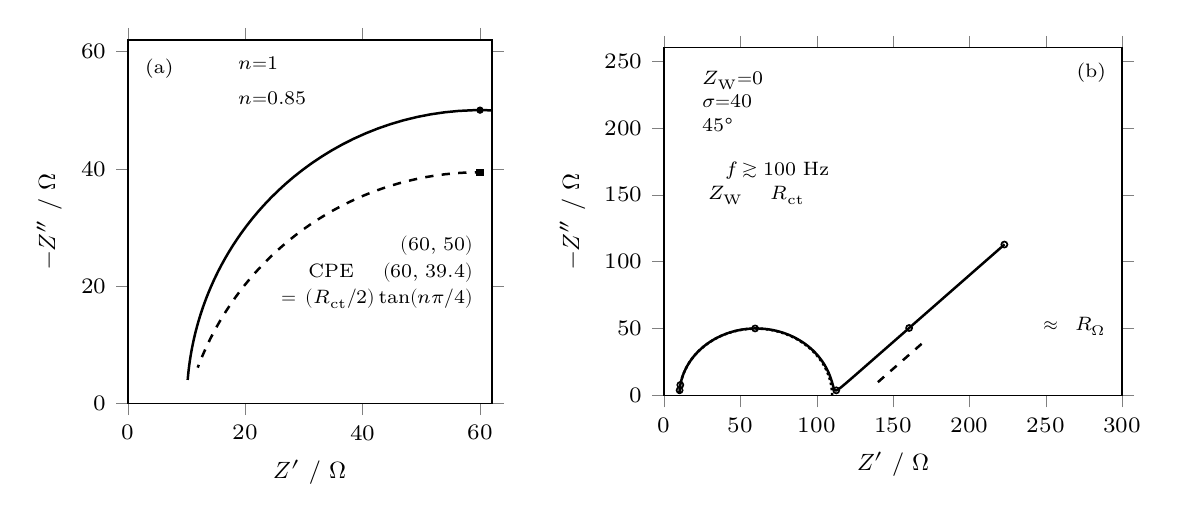
\begin{tikzpicture}
\tikzset{declare function={
  dpw(\z)  = 10^(\z);
  dwn(\z)  = 2*3.14159265358979*dpw(\z);
  dtc(\z)  = 100*0.5e-6;
  dpr(\z)  = dwn(\z)*dtc(\z);
  didx(\z) = 10+100/(1+(dpr(\z))^2);
  didy(\z) = 100*dpr(\z)/(1+(dpr(\z))^2);
  dq0      = (0.5e-6)^(0.85)*100^(0.85-1);
  dcpn     = 0.85;
  % 角度一律用「度」：pgfmath 的 sin/cos/tan 取度不取弧度（R3-C02 的实测探针
  %   sin(0.85*pi/2)=0.02328 是 sin(1.335°) 的值）。原先写 dcpb=n*pi/2 等于把
  %   θ 当成 1.335 rad 用，sin/cos 全部算错，弧被压成一条贴着横轴的线。
  dcpb     = dcpn*90;
  % u = Rct*Q*ωⁿ 才是无量纲组合；原写法 (ω*100*Q)^n 把整个乘积升到 n 次，
  %   量纲和数值都不对。下面的 a、d 分别是分母 1+u(cosθ+j sinθ) 的实部与虚部。
  dcpu(\z) = 100*dq0*(dwn(\z))^(dcpn);
  dcpa(\z) = 1+dcpu(\z)*cos(dcpb);
  dcpd(\z) = dcpu(\z)*sin(dcpb);
  dcpx(\z) = 10+100*dcpa(\z)/((dcpa(\z))^2+(dcpd(\z))^2);
  dcpy(\z) = 100*dcpd(\z)/((dcpa(\z))^2+(dcpd(\z))^2);
  % CPE 弧顶的解析值：对 u 求极值（u=1）得 Z'=Rs+Rct/2、-Z''=(Rct/2)tan(nπ/4)。
  %   标记点由这两个式子给出，不再手写孤立坐标。
  dcpxp    = 60;
  dcpyp    = 50*tan(dcpn*45);
  % Randles 加半无限 Warburg：Z = Rs + [1/(Rct+σ(1-j)/√ω) + jωC]^{-1}
  %   （式~\eqref{eq:eis-d-randles}）。原写法把它当成 Rct∥Warburg 的两元并联
  %   —— 丢失了 Cdl 支路 —— 并且把有量纲的 σ/√ω 直接与 1 相加（R3-C03 的根因）。
  %   下面改用归一化导纳 Ŷ = Y·Rct（无量纲）：
  %     t = σ/(Rct√ω)，S = (1+t)²+t²，Ŷ = (1+t)/S + j[t/S + ω C Rct]
  %   再取 Z - Rs = Rct/Ŷ。中间量都远离 pgfmath 的数值上下限，低频段也不会
  %   因为两个小量相减而丢精度。
  dkwz(\z) = 40/(100*sqrt(dwn(\z)));
  dkwS(\z) = (1+dkwz(\z))^2+(dkwz(\z))^2;
  dkwA(\z) = (1+dkwz(\z))/dkwS(\z);
  dkwB(\z) = dkwz(\z)/dkwS(\z)+dwn(\z)*0.5e-6*100;
  dkwN(\z) = (dkwA(\z))^2+(dkwB(\z))^2;
  dkwx(\z) = 10+100*dkwA(\z)/dkwN(\z);
  dkwy(\z) = 100*dkwB(\z)/dkwN(\z);
  % R2-C06：原先还声明过 dm / dmt / dmph / diph 四个量，已删除——
  %   ① 全书 grep 确认它们从未被任何 \addplot 调用（纯死代码）；
  %   ② 数学上也不成立：`diph` 给出的是 atan(ωRC)，按本节 φ≡−arg Z
  %      （tanφ=1/ωRC）恰是 φ 的余角；并且 pgfmath 的三角函数取「度」，
  %      要算 tan(76.5°) 就得写 tan(76.5)，写成 tan(dm*90) 之类是弧度思维。
  %   留着会被后来者当成可用函数，故删除而不是改写。本图不画相角曲线。
}}

\begin{axis}[
  name=eisda,
  width=70mm, height=62mm,
  unit vector ratio=1 1 1,
  xlabel={$Z'$ / $\Omega$}, ylabel={$-Z''$ / $\Omega$},
  % 轴伸到 62 Ω（刻度仍到 60），让两个弧顶标记落在框内而不是压在边框上。
  xmin=0, xmax=62, ymin=0, ymax=62,
  xtick={0,20,40,60}, ytick={0,20,40,60},
]
  \addplot[mainline,black,domain=0.3:4.9,samples=220,variable=\z]
    ({didx(\z)},{didy(\z)});
  \addplot[mainline,black,dashed,domain=0.3:4.9,samples=220,variable=\z]
    ({dcpx(\z)},{dcpy(\z)});
  \addplot[only marks,mark=*,mark size=1pt,black]
    coordinates {(60,50)};
  \addplot[only marks,mark=square*,mark size=1pt,black]
    coordinates {({dcpxp},{dcpyp})};
  \node[anchor=north west,font={\fontsize{7}{8.5}\selectfont}]
    at (axis cs:1.2,60.5) {(a)};
  % 曲线身份直接写在面板里（理想弧在 y>50 Ω 处、CPE 弧在 x>22 Ω 处都已是最上沿，
  %   这两处标注不会与任何曲线交叉）。图例因此取消，避免文字块压住弧顶。
  \node[anchor=west,font={\fontsize{7}{8.5}\selectfont}] at (axis cs:14,58) {实线 $n{=}1$};
  \node[anchor=west,font={\fontsize{7}{8.5}\selectfont}] at (axis cs:14,52) {虚线 $n{=}0.85$};
  % 说明块放进右下角的空白区（两条弧在 x>22 Ω、y<15 Ω 处都没有线），
  %   不再放到坐标区外，避免被裁掉。
  \node[anchor=south east,align=right,text width=28mm,font={\fontsize{7}{8.5}\selectfont}]
    at (axis cs:60.5,14.5)
    {理想弧顶点 $(60,\,50)$\\[1pt]
     CPE 弧顶点 $(60,\,39.4)$\\[1pt]
     $=(R_{\mathrm{ct}}/2)\tan(n\pi/4)$};
\end{axis}

\begin{axis}[
  name=eisdb,
  at={(eisda.right of east)}, anchor=left of west, xshift=6mm,
  width=74mm, height=60mm,
  xlabel={$Z'$ / $\Omega$}, ylabel={$-Z''$ / $\Omega$},
  xmin=0, xmax=300, ymin=0, ymax=260,
  xtick={0,50,100,150,200,250,300}, ytick={0,50,100,150,200,250},
]
  \addplot[mainline,black,densely dotted,domain=0.3:5.4,samples=300,variable=\z]
    ({didx(\z)},{didy(\z)});
  \addplot[mainline,black,domain=-1.7:5.4,samples=320,variable=\z]
    ({dkwx(\z)},{dkwy(\z)});
  % 六个读图点的坐标同样来自上面的函数（log10 f = -1.69897、-1、1.50515、
  %   3.50515、4.60206、4.90309，即 0.02 Hz、0.1 Hz、32 Hz、3.2 kHz、40 kHz、
  %   80 kHz），不是手写读数。
  \addplot[only marks,mark=o,mark size=1.1pt,black,mark options={fill=white}]
    coordinates {({dkwx(-1.69897)},{dkwy(-1.69897)})
                 ({dkwx(-1)},{dkwy(-1)})
                 ({dkwx(1.50515)},{dkwy(1.50515)})
                 ({dkwx(3.50515)},{dkwy(3.50515)})
                 ({dkwx(4.60206)},{dkwy(4.60206)})
                 ({dkwx(4.90309)},{dkwy(4.90309)})};
  % 45° 参考线只画一小段，放在扩散尾下方、说明块左侧的空白处（原先横跨全图，
  %   从三块说明文字上穿过去 —— R3-U01）。
  \addplot[mainline,black,dashed] coordinates {(140,10) (170,40)};
  \node[anchor=north east,font={\fontsize{7}{8.5}\selectfont}]
    at (axis cs:296,256) {(b)};
  % 面板 (b) 里最高的一条曲线只到 112.8 Ω，故 y>150 Ω 的整条带都是空白。
  \node[anchor=north west,align=left,text width=30mm,font={\fontsize{7}{8.5}\selectfont}]
    at (axis cs:8,250)
    {点线：$Z_{\mathrm{W}}{=}0$\\ 实线：$\sigma{=}40$\\ 虚线：$45$° 参考线};
  % 两块说明都落在空白区：上方（y>120 Ω 无曲线）与右下方（扩散尾下方）。
  \node[anchor=north west,align=left,text width=34mm,font={\fontsize{7}{8.5}\selectfont}]
    at (axis cs:8,182)
    {实线与点线在 $f\gtrsim 100$ Hz 几乎重合：只看高频段，\\ 分不开「$Z_{\mathrm{W}}$ 大」与「$R_{\mathrm{ct}}$ 大」};
  \node[anchor=south east,align=right,text width=22mm,font={\fontsize{7}{8.5}\selectfont}]
    at (axis cs:296,6)
    {高频截距 $\approx R_{\Omega}$\\ 只在弧闭合、\\ 无电感时成立};
\end{axis}
\end{tikzpicture}
\caption{三类等效电路的 Nyquist 图对照（模型计算）。取
$R_{\Omega}=10$ \unit{\ohm}、$R_{\mathrm{ct}}=100$ \unit{\ohm}、
$C_{\mathrm{dl}}=0.5$ µF（$\omega_{\max}=1/(R_{\mathrm{ct}}C_{\mathrm{dl}})$
对应 $f_{\max}\approx3.2$ kHz）；CPE 取 $n=0.85$、
$Q=C_{\mathrm{dl}}^{\,n}R_{\mathrm{ct}}^{\,n-1}\approx2.21\times10^{-6}$ S·s$^{0.85}$，
即低频极限电容与理想情形相同；Warburg 取 $\sigma=40$ \unit{\ohm.s^{-1/2}}。
三条曲线（实线、虚线、点线）分别由式~\eqref{eq:eis-d-randles}、
式~\eqref{eq:eis-d-cpe}、式~\eqref{eq:eis-d-rc} 按同一组参数算出：图中两个弧顶标记与
六个空心圆点都是这些函数的取值，不是手工写上的读数。
\textbf{(a)} 只画 $f=2$ Hz 至 79 kHz、$Z'\le62$ \unit{\ohm} 的窗口（两条弧的右半段落在
窗口外）：理想弧（$n=1$）的顶点在
$(R_{\Omega}+R_{\mathrm{ct}}/2,\;R_{\mathrm{ct}}/2)=(60,\,50)$，CPE 弧的顶点在
$(60,\,39.4)$——\textbf{横坐标相同，纵坐标只有 $(R_{\mathrm{ct}}/2)\tan(n\pi/4)$；
同样一个 $R_{\mathrm{ct}}$、同样一个低频极限电容，仅因 $n=0.85$ 就把弧的高度压到
$0.79$ 倍，而顶点频率并不改变}。两条曲线在 $f\to0$ 时都收敛到
$R_{\Omega}+R_{\mathrm{ct}}=110$ \unit{\ohm}（点线在 (b) 中可见 $10\to110$ \unit{\ohm}
的完整弧；CPE 弧的右半段落在 (a) 的窗口之外）。
\textbf{(b)} 频率 0.02 Hz 至 250 kHz：实线在 $f\lesssim 10$ Hz 之后已明显
偏离点线，朝向 $45$°参考线（虚线）——但\textbf{即使在 40 kHz，实线的截距仍是
10.6 \unit{\ohm} 而非 10.0 \unit{\ohm}、相角仍有 $+36.6$°（按 $\varphi\equiv-\arg Z$），即高频平台并未形成}，
这正是规则一第（1）条的量化含义；六个空心圆点依次标出后文读图实例所用的频率
（80 kHz、40 kHz、3.2 kHz、32 Hz、0.1 Hz、0.02 Hz），可以逐点核对。
注意 (b) 两个坐标轴的刻度尺度不同（横轴 300 \unit{\ohm} 与纵轴 260 \unit{\ohm}
画在等宽的图面上），故 $45$°参考线在图上并不呈 $45$°；判斜率请用数值而非图面角度。
局限：本图不含接触电阻、引线电感、有限扩散与吸附弛豫，真实数据在高频端与最低频端都会多出
本图没有的结构。
\modelmark\pedset{$R_{\Omega}$、$R_{\mathrm{ct}}$、$C_{\mathrm{dl}}$、$n$、$\sigma$ 为教学设定，
按式~\eqref{eq:eis-d-randles}、式~\eqref{eq:eis-d-warburg}、式~\eqref{eq:eis-d-cpe} 计算。}
\figsrc{结构取自 S2 §11.5.1 对四类电极 Nyquist 图与原书表 11-1 的论述
（书内 p.859—861 / PDF p.347—349）；具体数值为模型计算，非原书数据。}}
\label{fig:eis-d-model}
\end{figure}

\paragraph{读图实例：在一张模型 Nyquist 图上依次读出三类信息} 下面用图~\ref{fig:eis-d-model}
的数据走一遍完整读图流程。把\textbf{观察}与\textbf{推断}严格分开，因为这里的每一步推断都依赖
一个前提。

\begin{obs}
在图~\ref{fig:eis-d-model}(b) 的实线（含 Warburg）上（六个空心圆点即下列读数，
按频率从高到低排列）：
（1）从最高频端（80 kHz）开始，曲线左端落在 $Z'\approx 10.16$ \unit{\ohm}、
$-Z''\approx 3.97$ \unit{\ohm} 处，并未落在实轴上；
（2）频率降到 40 kHz 时 $Z'\approx 10.63$ \unit{\ohm}、$-Z''\approx 7.91$ \unit{\ohm}：
截距几乎没变，$-Z''$ 却翻了一倍；
（3）频率降到约 3.2 kHz 时，$-Z''$ 达到极大值约 50.1 \unit{\ohm}，此时
$Z'\approx 59.6$ \unit{\ohm}；
（4）继续降频，$-Z''$ 先减小到约 3.9 \unit{\ohm}（$f\approx 32$ Hz，此时
$Z'\approx 112.8$ \unit{\ohm}），再转而增大；
（5）在 $f\lesssim 10$ Hz 之后，$Z'$ 与 $-Z''$ 同步增大，在
0.1～0.02 Hz 段内 $Z'$ 从 160 \unit{\ohm} 增至 223 \unit{\ohm}、
$-Z''$ 从 50 \unit{\ohm} 增至 113 \unit{\ohm}，两点连线的斜率约为 $1.00$；
（6）把 (b) 中的点线（无扩散）与实线对比：两条线在 $f\gtrsim 100$ Hz 时肉眼不可分，
分岔从约 30 Hz 开始，到 0.02 Hz 时点线停在 $Z'=110$ \unit{\ohm}、
$-Z''\approx0$，而实线已走出 223 \unit{\ohm} 之外。
在 (a) 中对比理想弧（实线）与 CPE 弧（虚线）：两条弧的高频端都趋向同一点
（$Z'=R_{\Omega}$），低频端都趋向 $Z'=R_{\Omega}+R_{\mathrm{ct}}$（两端位置与 $n$ 无关），
但中段完全分开——理想弧顶点 $(60,\,50)$，CPE 弧顶点 $(60,\,39.4)$，后者只有前者的
$0.79$ 倍高，而顶点频率同为 $3.2$ kHz。
\end{obs}

\begin{infer}
（1）高频端不落在实轴上、且 $-Z''$ 仍有 4.0 \unit{\ohm}，说明\textbf{最高频处高频平台
尚未形成}，因此 (b) 左端那个 10.16 \unit{\ohm} \textbf{不能直接当作 $R_{\Omega}$}：
照读会把溶液电阻高估约 $1.6\%$；若改用 40 kHz 的读数 10.63 \unit{\ohm}，高估量升到
$6.3\%$。（该值是否可读，判据是 Bode 图上 $|Z|$ 与 $\varphi$ 是否出现平台。）
（2）极化电阻以弧的形式出现，说明该频段由电荷转移与双电层构成的\textbf{并联}支路支配；
在扩散尚未参与的高频段，这段弧的直径给出 $R_{\mathrm{ct}}$：理想弧的直径
$110-10=100$ \unit{\ohm}，与设定值一致。顶点条件
$\omega_{\max}=1/(R_{\mathrm{ct}}C_{\mathrm{dl}})$ 反过来给出
$C_{\mathrm{dl}}=1/(2\pi\times3183\times100)\approx0.5$ µF，也与设定值一致——
\textbf{但这两个数能读对，是因为本例恰好是完整半圆；换成 (a) 中的 CPE 弧，
用「直径」读 $R_{\mathrm{ct}}$ 仍得 100 \unit{\ohm}（两端截距与 $n$ 无关），
而用「弧顶高度 $=R_{\mathrm{ct}}/2$」读就只有 $2\times39.4=79$ \unit{\ohm}，
再代入 $C=1/(\omega_{\max}R_{\mathrm{ct}})$ 得 $0.63$ µF——与真值分别差 $21\%$ 与
$27\%$。压扁的弧不满足式~\eqref{eq:eis-d-rc} 的圆方程：顶点高度是
$(R_{\mathrm{ct}}/2)\tan(n\pi/4)$，不是 $R_{\mathrm{ct}}/2$。}
（3）$-Z''$ 先减到极小再增大，是本图上最容易被忽略的特征：极小值点的出现说明\textbf{有两个
不同时间尺度的过程串接在同一支路上}——高频弧（电荷转移）在约 30 Hz 处已衰减完毕，
而扩散项在更低频处才开始主导。因此「$-Z''$ 极小点」的位置是判断两个过程是否已分离的实用标志。
（4）低频段 $Z'$ 与 $-Z''$ 同步增大且连线斜率约 $1.00$，与式~\eqref{eq:eis-d-warburg}
的 $Z'_{\mathrm{W}}=-Z''_{\mathrm{W}}$ 一致，故该段可归为\textbf{半无限线性扩散（Warburg 阻抗）
控制}。斜率也因此是判断「扩散段是否已经独立」的实用判据：若把拟合区间一直取到弧上
（例如 3.2 kHz 与 0.02 Hz 两点连线，斜率只有约 $0.38$），正在衰减的电荷转移弧会把斜率
大幅拉低——\textbf{用斜率反算 $\sigma$ 必须先扣掉弧的贡献}。
（5）(b) 中点线与实线的分岔起点约 30 Hz，正是「扩散开始参与」的频率；而两条线在
$f\gtrsim 100$ Hz 不可分，说明\textbf{只看高频段的数据无法判断体系有没有扩散}。
这给出频率范围要求的一个定量形式：低频端必须至少比这个分岔频率低两个数量级，扩散尾才成形。
（6）(a) 中两条弧的高频端与低频端重合、中段分开，说明\textbf{弧的「两端」不携带
$n$ 的信息}——端点是 $R_{\Omega}$ 与 $R_{\Omega}+R_{\mathrm{ct}}$，与 $n$ 无关。因此
「用低频截距减高频截距得 $R_{\mathrm{ct}}$」这条做法即使在 CPE 情形下也成立
（本例中两条弧都给出 100 \unit{\ohm}）；\textbf{出错的是把中段几何（顶点高度、半高处宽度）
当作 $R_{\mathrm{ct}}/2$ 与 $1/(R_{\mathrm{ct}}C_{\mathrm{dl}})$ 去用}。
\end{infer}

\begin{pitfall}
\textbf{（1）拟合优度高不等于电路唯一。} 这是等效电路拟合的第一风险，也是本节所有其它风险的
放大器。\textbf{不同的电路可以对同一组数据给出几乎相同的拟合曲线}——只看图~\ref{fig:eis-d-model}(a)
的中段，同一段压扁的弧（跨度 $110-10=100$ \unit{\ohm}、顶点高 $39.4$ \unit{\ohm}）
至少可以用三种完全不同的电路拟合：①CPE（$n=0.85$）加 $R_{\mathrm{ct}}=100$ \unit{\ohm}；
②两个时间常数相差 $4$ 倍的 $(R\parallel C)$ 串联（各 $50$ \unit{\ohm}，即把这一段
100 \unit{\ohm} 拆成 $50+50$——峰值仍在 $3.2$ kHz、峰高 $40.0$ \unit{\ohm} 与
$39.4$ \unit{\ohm} 几乎相同，全频段与①的差别不超过约 $3$ \unit{\ohm}）；
③单个理想 $(R\parallel C)$ 串一个扩散项。三者的残差都可以做到很小，而它们给出的
「$R_{\mathrm{ct}}$」可以是 100 \unit{\ohm}（①）、两个各 50 \unit{\ohm}（②）、
或按弧顶高度误读出的 79 \unit{\ohm}——相差一倍以上。
\textbf{残差小只说明该电路在数值上能复现数据，不代表它对应真实的物理过程}。实践判据：换一组
完全不同的初值（或换一个拓扑相近的电路）重新拟合，若参数漂移到另一个解而残差几乎不变，就说明
该解不可辨识；此时只能报告「表观值」并把候选机理并列写出。

\textbf{（2）参数相关性使单个参数失去意义。} 这是风险（1）的数学根源。CPE 的 $Q$ 与 $n$ 高度
相关（$n$ 略变，$Q$ 可补偿性地变几个数量级）；$R_{\Omega}$ 与 $R_{\mathrm{ct}}$ 在同一数量级时
互相补偿；两个时间常数接近时，$R_{1}$、$C_{1}$、$R_{2}$、$C_{2}$ 四者其实只是两个可辨识的
组合量。因此\textbf{必须报告参数的置信区间与相关系数矩阵}——只报一组「最优值」而不报不确定度，
等于没有报告结果。报告 $Q$ 与 $n$ 时必须同时给出换算成电容所用的式子
（式~\eqref{eq:eis-d-cpeceff}），否则读者无法复算。

\textbf{（3）把 Warburg 当半圆。} 半无限扩散的 $45$°直线在只测到一段时很像大半径圆弧的一部分；
图~\ref{fig:eis-d-model}(b) 的实线在 10 Hz 以下那一段若单独放大，斜率 $1.00$ 的
「直线」完全可以被一个半径很大的圆拟合。直接按半圆读直径会把 $R_{\mathrm{ct}}$ 高估几倍。
\textbf{判别办法是换到 Bode 图}：扩散段的 $|Z|$ 应呈 $\omega^{-1/2}$、相角应稳定在约 $+45$°，
而圆弧段的相角会扫过一整段。

\textbf{（4）频率范围不够就下结论。} 图~\ref{fig:eis-d-model}(b) 已经给出量化例子：两条曲线
（有扩散／无扩散）在 $f\gtrsim 100$ Hz 不可分，在 40 kHz 处连高频平台都还没
形成。起始频率不够高，截距含 $R_{\mathrm{ct}}$，$R_{\Omega}$ 偏大；终止频率不够低，看不到扩散
尾或第二个弧，于是把「没看到」当成「不存在」，进而误判速控步。\textbf{频率范围不是实验参数，
它是结论的适用范围}，必须与结论一起报告。

\textbf{（5）把 CPE 当理想电容算电容值。} 这是最常见的一个算术错误，且\textbf{不报错、不告警}。
$Q$ 的量纲是 $\mathrm{S.s^{n}}$，$n=0.85$ 时 $Q=2.21\times10^{-6}$ 与同体系的
$C_{\mathrm{dl}}=0.5$ µF 相差 $4.4$ 倍，而且量纲不同——直接拿 $Q$ 当作电容会高估四倍以上；
式~\eqref{eq:eis-d-cpeceff} 的换算是必须做的。另一个同源错误是把
$C_{\mathrm{dl}}=1/(\omega_{\max}R_{\mathrm{ct}})$ 直接用在压扁的弧上——如图~\ref{fig:eis-d-model}(a)
所示，把弧顶高度当 $R_{\mathrm{ct}}/2$ 会读成 $R_{\mathrm{ct}}\approx79$ \unit{\ohm}，
代入后得 $0.63$ µF（真值 0.5 µF，高 $27\%$）；压得越扁，误差越大。
\textbf{只要 $n<0.95$，就不要用几何法读电容。}

\textbf{（6）未扣除溶液电阻。} $R_{\mathrm{ct}}$ 必须是在扣除 $R_{\Omega}$ 之后读出的弧直径；
用未校正的过电位去算动力学参数，误差随电流密度线性放大。更隐蔽的是：$R_{\Omega}$ 随电解质
浓度、电极间距与温度变化，\textbf{每次实验都应重新读，不能沿用上一批的值}。

\textbf{（7）把接触阻抗当电荷转移阻抗。} 电极与集流体、催化剂层与膜之间的接触电阻，以及参比
电极的鲁金毛细管位置不当引起的未补偿电阻，都会并入高频段，被拟合成一个大 $R_{\mathrm{ct}}$ 或
一个低 $n$ 的 CPE。这与（1）的危险叠加：接触电阻造成的低 $n$ 会被解释成「表面不均匀」这一
化学结论。\textbf{判别办法：改变电极压紧力或参比位置，若该「$R_{\mathrm{ct}}$」或「$n$」跟着
变，它就不是化学信息}。

\textbf{（8）稳态未建立就测。} 阻抗定义要求体系在测量期间是线性时不变系统。刚跳到目标电位、
表面覆盖度还在漂移、或催化剂正在失活时测得的谱，会在低频段出现「漂移型」假弧——而低频段恰好
是耗时最长、也最容易被漂移污染的一段。判据见「测量条件」第（5）条：先在单一频率上监测
$\lvert Z\rvert$ 的时间稳定性，再做全谱扫频；同一电位下正扫与反扫各测一次，两条谱重合才说明
稳态已建立。

\textbf{（9）扰动幅度过大。} 幅度过大会使响应非线性，Kramers--Kronig 检验不通过，并系统性
压低 $R_{\mathrm{ct}}$——因为大信号下电流–电势关系不再是线性的，等效电路这一整套线性工具
（包括式~\eqref{eq:eis-d-randles}）全部失效。用幅度减半检验把关。

\textbf{（10）把 $f_{\max}$ 当作 $\omega_{\max}$ 代入。} 式~\eqref{eq:eis-d-cdl} 中的
$\omega$ 是角频率。用 Hz 为单位直接代入会得到错 $2\pi$ 倍（约 $6.28$ 倍）的电容值。这是一个
纯粹的记账错误，但因为结果「看起来合理」，很少被当作可疑值复查。
\end{pitfall}

\begin{crosscheck}
阻抗谱给出的归属结论不应单独成立，至少与下列方法之一互查——每条互查针对的是\textbf{同一组
数据的一个具体参数}，而不是笼统地「再测一次」：

\textbf{（1）$R_{\mathrm{ct}}$ 对稳态极化／Tafel 斜率。} 在小过电位下
$R_{\mathrm{ct}}=RT/(nFi_0)$，因此由弧直径反推的 $i_0$ 应与 Tafel 外推值同数量级；差一个数量级
以上就说明弧里混了别的贡献（接触电阻、扩散、或第二个时间常数）。
\tocheck{未对照原页面图像：$R_{\mathrm{ct}}$ 与 $i_0$ 的换算关系式及电子数 $n$ 的约定按学科
标准形式给出，源文本 §11.5.1 未给出该式，须与页面核对。}

\textbf{（2）扩散项对旋转圆盘变转速。} 扩散控制的阻抗应在提高转速后缩短低频尾（边界层变薄），
而电荷转移控制的弧几乎不变。这条互查把 Warburg 与半圆分开，且不依赖任何模型假设——是本节最
有力的一条独立判据。RDE 的 Levich 斜率与阻抗 $\sigma$ 还可交叉校核同一个 $D$
（\S 11.4.2）。

\textbf{（3）$C_{\mathrm{dl}}$ 对循环伏安的电容电流。} 在无法拉第电流的电位区间做不同扫速的
循环伏安，由 $\mathrm{d}i/\mathrm{d}v$ 得到电容，应与阻抗高频弧给出的电容一致；两者一致才说明
高频弧确由双电层充电支配。

\textbf{（4）$R_{\Omega}$ 对电流中断法或正反馈补偿。} $R_{\Omega}$ 是阻抗谱最不可靠的一个数
（见「误判」第 6、7 条），必须用独立方法标定。三个值一致时，高频截距的归属才算落实。

\textbf{（5）时间常数个数对机理中的独立状态变量个数。} 源文本强调，从阻抗谱中时间常数的个数
及其数值大小可以获得各个步骤的动力学信息与电极表面状态变化的信息，还可观察电极过程中有无传质
过程的影响\src{书内 p.856 / PDF p.344}。把这条当作系统性的自检：\textbf{Bode 相角图上数出的
峰个数，应与所假定机理中独立状态变量的个数一致}；多了说明电路里塞进了不存在的元件，少了说明
两个过程的时间常数重叠、当前电路无法分辨它们。

\textbf{（6）与其它分片的一致性。} 本节是同一章内给出阻抗基本定义与 $Z$ 与元件关系的地方，
因此它与下一节（§11.5，电化学阻抗谱的应用与读图）的接口必须一致：\textbf{（i）}$R_{\Omega}$
的符号与含义（分片 c 沿用源文本符号 $R_{\mathrm{s}}$，指同一量）；\textbf{（ii）}Nyquist 图
纵轴取 $-Z''$ 的约定；\textbf{（iii）}相角取测量约定 $\varphi\equiv-\arg Z$（容性为正，纯电容
$+90$°、感性为负——分片 c 的读图实例即按此约定写「相角接近 $90$°」与「第四象限的负相角」）；
\textbf{（iv）}$\omega_{\max}$ 而非 $f_{\max}$ 用于
式~\eqref{eq:eis-d-cdl}。四处中任何一处不一致，读图结论就无法互相引用。

装配顺序已在 \texttt{chapters/ch11.tex} 中按文件头注释的处置办法（A）修正：本分片现排在
§11.4（分片 b）之后、§11.5 与 §11.6（分片 c）之前，故上文的「读图规则」在下文中确为
\textbf{上文}，§11.5.1 与 §11.5 的先后关系与实际排版一致。两分片之间原有一批重复段落
（阻抗定义与两种画法、等效元件表、三条读数规则、误判清单、测量条件），合并时按
\textbf{保留有源文本页码依据的一侧}处理：这些内容一律以本分片为准，分片 c 只保留
源文本 §11.5.2 特有的读图实例（甲醇氧化）与互补回查，不再重复。
\end{crosscheck}
}{}
\IfFileExists{chapters/parts/ch11-c.tex}{\subsection{电化学阻抗谱}

稳态极化曲线把所有步骤的过电位加总成一个数；阻抗谱则用一串不同频率的小幅正弦扰动，把总响应按\textbf{时间尺度}拆开——快步骤（溶液电阻、双电层充电）在高频段显现，慢步骤（电荷转移、吸附、扩散）在低频段显现\src{S2 §11.5，书内 p.866 / PDF p.354}。分段能力是它最大的价值，也是它最大的风险来源：把频率轴上某一段的形状直接翻译成一个元件，很容易得到「拟合优度很高、物理归属却错」的电路。

本分片源文本自书内 p.866（PDF p.354）起，只包含 §11.5 的后半（应用与读图）与 §11.6 全节；阻抗的基本定义、等效电路推导与 Nyquist／Bode 图的定义在源书 §11.5.1，不在本分片的源文本范围内——它们在前一节（§11.5 阻抗谱基本原理，依源文本写成，标有 \src{} 依据）。下文凡标 \tocheck{} 处，即按学科标准形式重建、未能与源文本对齐的部分。

\begin{probout}
 已知：电极过程的总电流至少含溶液电阻、双电层充电、电荷转移、吸附中间体与扩散五类贡献，稳态方法只能给出它们的总和。
 要问：能否把总响应分解成若干时间常数，分别读出溶液电阻 $R_{\mathrm{s}}$、双电层电容 $C_{\mathrm{dl}}$、电荷转移电阻 $R_{\mathrm{ct}}$ 与扩散阻抗，并据此判断哪一步是速率控制步骤？
 要给出：覆盖足够宽频率范围的一组阻抗数据、一个（或几个）能同时拟合全部频率的等效电路，以及每个参数的物理归属与成立条件——并明确「能拟合」不等于「唯一」。
\end{probout}

\subsubsection{读图实例：甲醇氧化的阻抗谱随电位的变化}

上一节（源书节号 §11.5.1，本项目中即紧接在前的一节）已给出阻抗的定义 $Z(\omega)=E(\omega)/I(\omega)$、Nyquist／Bode 两种画法、等效元件的来源与四类电极的特征谱，以及「高频截距」「半圆直径」「低频 45°斜线」三条读数规则各自成立的条件；本节不再重复，只处理源文本 §11.5.2 的真实数据。

源文本用同一组数据的两套图讨论甲醇在铂系催化剂上的氧化：Nyquist 形式的图 11-42 与以相角为主的图 11-43\src{S2 §11.5.2，书内 p.866 / PDF p.354}。下面把\textbf{观察}与\textbf{推断}严格分开，因为这里的每一步推断都依赖一个前提。

\begin{obs}
随直流电位升高，阻抗谱按四个区间改变形状：
（1）$0.10\sim0.20$ V：谱几乎是一条沿虚轴、相角接近 $90$° 的直线；
（2）$0.20\sim0.33$ V：相角迅速下降，但仍在 $0$° 以上，低频区近似电阻行为；谱线略偏离虚轴；
（3）$0.35$ V 起：谱延伸进第四象限，出现负相角（电感现象）；在 $0.35\sim0.48$ V 区间，电感行为位于低频区，且各条曲线随电位升高整体向高频方向移动；
（4）$0.48$ V 以上：谱突变，分裂为两段分离的曲线，高频段相角越出 $90$°。
但图中纵横坐标与相角的具体数值需对照原书图 11-42、图 11-43\tocheck{未对照原页面图像：源文本对 0.48 V 以上的描述两次出现「超过 90°」（高频段与低频段），疑为 OCR 重复或原文指低频段相角亦越出 0—90° 区间；图的纵轴定义（$-Z''$ 或相角／°）与频率范围无法在本分片源文本内确认}。
\end{obs}

\begin{infer}
（1）接近虚轴且相角接近 $90$° 的直线是理想极化电极（纯电容）特征：在这个电位区间几乎没有法拉第电流，电极／溶液界面只表现为双电层充电。
（2）相角下降而不越过 $0$°，说明出现了耗散性的法拉第通道；谱线开始偏离虚轴，与甲醇离解吸附的开始相对应。
（3）第四象限的负相角是电感行为，源文本把它归属于强吸附中间体 \ce{CO_{ad}} 的吸附弛豫。判据是\textbf{出现电位区间}与已知的 CO 吸附电位区间一致，而不是单看形状——仪器电感也会给第四象限，见下文误判清单第（1）条「第四象限的电感弧」。
（4）源文本采用的判断规则是：\textbf{低频区的过程是速率控制步骤}；因此随电位升高曲线向高频方向移动，就意味着该低频过程的速率在加快。据此，$0.35$ V 以前低频区为电阻行为、速控步是甲醇的离解吸附；$0.35\sim0.48$ V 低频区为电感行为、速控步是生成 \ce{CO_{ad}} 的步骤；$0.48$ V 以上低频区转为钝化行为、速控步是 \ce{CO_{ad} -> CO2}。谱在 $0.48$ V 的突变因此被解释为「CO 的生成与消耗两个步骤中，速控步发生了转移」。
（5）与上一条互补的判据是\textbf{斜率的数值}：$-Z''$ 对 $Z'$ 的斜率明显小于 $45$°（例如落在 $20$°～$30$°）时，通常意味着扩散层已「看到」边界、不再满足半无限扩散的前提，或有吸附弛豫叠加在扩散尾上——此时不能把该段直接当 Warburg 处理。这条判据只在频率范围够低、确实取到了扩散段之后才有意义。
\end{infer}

\begin{dataflow}
从一组阻抗数据到「速控步是谁」的完整链条中，\textbf{检验}（正反扫重合、Kramers--Kronig 残差）与\textbf{数时间常数}（Bode 相角图数峰）两步已写在上一节（源书 §11.5.1），此处不重复；真实数据特有的三步是：
（1）\textbf{定元件归属}——高频截距给 $R_{\mathrm{s}}$，最低频的极限行为决定是扩散（45°）、吸附（低频电容／电感弧）还是钝化（低频大电阻）。
（2）\textbf{跨电位比较}——只有同一套电路、同一套初值在全电位区间内都收敛，才能用「曲线向高频移动」这类趋势论证速率变化。
（3）\textbf{互查}——用独立实验（Tafel 斜率、变转速、原位谱学的覆盖度）验证归属，清单见下文；其中 Tafel 斜率与变转速两条属通用判据，已在上一节的互查清单里连同判据给出。
\end{dataflow}

\subsubsection{拟合的最大风险：参数相关性，以及「拟合好 $\neq$ 电路唯一」}

等效电路拟合的第一风险是\textbf{拟合优度高不等于电路唯一}：不同的电路可以对同一组数据给出几乎相同的拟合曲线。因此逐条列出误判清单仍有必要，尤其是下面几条在真实数据里最容易发生。判据、公式与量化例子见上一节的「误判」清单（十条），此处只列真实数据读图中另有表现的三条：

\paragraph{第四象限的电感弧}引线电感与强吸附中间体（如 \ce{CO_{ad}}）的吸附弛豫都给第四象限的弧。判别办法是改变接线方式或电极几何：\textbf{仪器电感应与频率无关、且能靠改接线消掉}；化学吸附弛豫则出现在确定的电位区间（如读图实例中的 $0.35\sim0.48$ V）。
\paragraph{吸附弛豫与双电层的重叠}吸附中间体的 $R_{\mathrm{ad}}$、$C_{\mathrm{ad}}$ 与 $C_{\mathrm{dl}}$ 的时间常数接近时，二者在 Nyquist 图上不可分辨，只能合并成一个压扁的弧（如读图实例中的甲醇体系）。此时单靠阻抗谱无法把覆盖度信息与双电层信息分开，必须引入原位谱学的覆盖度数据。
\paragraph{薄层与原位谱学联用时的第三套条件}若阻抗数据要与同一电位点的原位红外／拉曼对照，薄层电解池把传质条件改掉了，阻抗谱给出的扩散尾与厚层体系并不相同；两套数据的「同一电位」只有在覆盖度都达到稳态时才是同一个表面状态。

\subsubsection{测量条件与互补回查}

\begin{measure}
 \textbf{稳态与幅度}：体系在目标电位达到稳态后再扫频（判据见上一节测量条件第（5）条）；交流幅度取原书图 11-42／11-43 图注的 AC $10$ mV，并做第（2）条的幅度减半检验。
 \textbf{频率范围}：本分片读图实例所用原书图 11-42／11-43 的图注为 $20$ mHz 至 $5$ kHz；通用范围与点数的分配原则见上一节的测量条件第（3）条与规则三（源书 §11.5.1：低频端的点数要按「能否分辨出 45° 斜率」来定，而不是按对数均匀取点）。
 \textbf{电位区间}：至少覆盖目标反应从「无法拉第电流」到「扩散／钝化控制」的完整区间，才能用趋势论证速控步的转移（如读图实例中的 $0.10\sim0.48$ V）。
 \textbf{测量模式}：低阻抗、大电流体系（燃料电池单池、电池）宜用恒电流模式，避免恒电位仪过载；高阻抗体系（修饰电极、半导体电极）宜用恒电位模式\supp{恒电位／恒电流两种模式的适用判据属 §11.5.2 的讨论范围，不在本分片源文本内，此处只给判据}。
 \textbf{谱学联用前的采样条件}：若要与原位红外／拉曼的同一电位点对照，必须先让电位在该点稳定足够长时间（覆盖度达到稳态），否则两套数据的「同一电位」并不是同一个表面状态。
\end{measure}

\begin{crosscheck}
 阻抗谱的归属结论不应单独成立，至少与下列方法之一互查。上一节的互查清单（六条：$R_{\mathrm{ct}}$ 对 Tafel 斜率、扩散项对旋转圆盘变转速、$C_{\mathrm{dl}}$ 对循环伏安电容电流、$R_{\Omega}$ 对电流中断法、时间常数个数对独立状态变量个数、以及与其它分片的一致性）中，前两条已在上一节连同判据一起给出，此处不重复；真实数据读图另有表现的是三条：
 \textbf{（1）变温}：$R_{\mathrm{ct}}$ 的 Arrhenius 图给出表观活化能，可与同反应在稳态方法下的活化能比较。
 \textbf{（2）原位谱学}：第四象限的电感行为、低频吸附电容，应与原位红外／拉曼给出的 \ce{CO_{ad}} 覆盖度在同一电位区间出现——形状与分子信息对上了，归属才算落实。
 \textbf{（3）时间常数个数}：源文本强调，从阻抗谱中含有的时间常数个数及其数值大小可以推测电极过程的状态变量的情况，也可以观察电极过程中有无传质过程的影响，并由此得到溶液电阻、双电层电容及电极反应电阻等信息、推测反应机理\src{S2 §11.5，书内 p.866 / PDF p.354}（与上一节所引源书 p.856 处是同一条判据的两个出处）。把这条当作系统性的自检：时间常数个数应与你假定的机理中的独立状态变量个数一致，多了或少了都说明电路选错。
\end{crosscheck}

\subsection{电化学原位谱学技术}

常规电化学方法测的是界面上电流对电势或时间的响应，得到的是界面反应的综合信息，无法在分子水平上验证反应物、中间物种与产物，这给机理验证造成根本困难。原位谱学把谱学技术与电化学方法\textbf{同步}结合：在得到电流、电势等电化学信息的同时获得分子水平的信息，用于研究电极过程机理、电极表面特性、检测中间物种与产物、测定转移电子数、确定速率常数与扩散系数\src{S2 §11.6，书内 p.866—867 / PDF p.354—355}。本节按源文本的四个方面介绍：原位红外、原位拉曼、原位质谱与荧光单分子／单纳米粒子技术。

\begin{principle}
 原位（in situ）与离场（ex situ）的分界只有一条：\textbf{谱学测量是否在电化学调制进行的同时完成}。原位红外光谱电化学在反应体系被电化学调制与检测的同时监测红外信号变化；非原位红外则是在终止电化学反应之后对产物做红外研究\src{S2 §11.6.1，书内 p.867 / PDF p.355}。这一条分界决定了信息性质：原位方法能看到中间体与电位依赖，但必须解决「电解液对信号的干扰」与「传质受限」；离场方法信噪比与方法选择自由度大得多，但可能错过只在电位存在时才稳定的物种。
\end{principle}

\subsubsection{原位红外光谱电化学}

红外光谱电化学（infrared spectroscopy in electrochemistry）由红外光谱与电化学技术结合而成，可分为原位与非原位两类。原位红外既能检测电极表面吸附物种的身份与分子结构，也能探测电极表面及贴近表面薄液层中的反应物、产物与中间体，并为固／液界面提供双电层中物种的化学本质、成键方式及其随电位变化的信息。$1980$ 年 A. Bewick 等首次把电化学原位红外光谱成功用于电极／溶液界面研究，此后已建立的方法包括电化学调制红外光谱法（EMIRS）、差减归一化界面傅里叶变换红外光谱法（SNIFTIRS）、线性电位扫描反射光谱法（LPSIRS）、偏振调制红外光谱法（PMIRS）、傅里叶变换红外反射吸收光谱法（FTIRRAS）、时间分辨光谱电化学法（TRFTIRS）、二维红外光谱（2D-IR）与显微红外光谱电化学法（MFTIRS）等\src{S2 §11.6.1，书内 p.867 / PDF p.355}。

\begin{measure}
 \textbf{光路与窗口}：原位反射红外最常用外反射模式，红外辐射穿过窗口与溶液薄层，经研究电极表面反射后被检测。窗口材料必须对红外透明且不溶于所测溶液，如 \ce{CaF2}、\ce{Si}、\ce{ZnSe}。
 \textbf{薄层厚度是关键条件}：水及其他常用溶剂对红外辐射有强烈吸收，因此窗口与电极表面之间的液层必须很薄，约 $1\sim100$ nm。这一厚度同时决定了原位红外的时间响应与传质条件——薄层抑制了扩散，使本体浓度不再等于表面浓度，是原位红外定量结论的主要限制。
 \textbf{电极与池结构}：研究电极是封在玻璃或绝缘惰性材料中的圆盘，表面平整度要求高，固定在可调节电极与窗口距离的活塞末端，实验时充分接近窗口；通过调整反射镜角度选择最佳红外入射角，再用调制或差分技术取得最大检测信号\src{图 11-44、图 11-45，书内 p.868 / PDF p.356}。
\end{measure}

三种主要实验测试方式的差别在「减掉什么」上，理解这一点比记住缩写更重要\src{S2 §11.6.1，书内 p.868—870 / PDF p.356—358}：

\paragraph{EMIRS（电化学调制红外光谱）}
电势在「无研究物质产生」与「有电化学产物」两个位置之间以一定频率调制，用相敏检测器（PSD）解调，因而可以在测产物信号的同时排除溶剂与其他溶解物的吸收干扰，提高信噪比。测量的是电极电势由 $E_{1}$ 变为 $E_{2}$ 时表面相对反射率的改变量 $\Delta R$（相当于 $R(E_{2})-R(E_{1})$），最后以 $\Delta R/R$ 对波数作图。要点：\textbf{得到的是两个电位下的差谱}，因此单张谱不能直接给出绝对覆盖度。

\paragraph{SNIFTIRS（差减归一化界面傅里叶变换红外光谱）}
在傅里叶变换红外光谱基础上发展而来：单色仪被干涉仪取代，采集到的是强度随干涉仪物镜位置变化的干涉图；优点是可以多次采集并累加干涉图以提高信噪比。它测量两个不同电势下的谱图信号（电势分别取在所测物种的电化学过程发生与不发生处），在相应波长处作吸光度差减，再由计算机处理得到差谱。与 EMIRS 相比，它牺牲了调制解调的实时性，换来了可在宽波数范围同时取谱与更好的信噪比。

\paragraph{IRRAS（红外反射吸收光谱）}
依据红外反射光谱的表面选律：只有当吸附分子的偶极矩在电极表面法线方向上的分量不为零时，才能吸收平行于入射面的红外能量。装置上用光弹性调制器把入射光的偏振在 P 偏振与 S 偏振之间调制：P 光平行于入射面，可被电极表面与环境吸收；S 光垂直于入射面，不能与表面吸附物种相互作用，只包含环境对红外光的吸收。因此 P 光与 S 光的反射光谱之差就给出表面粒子的红外吸收信息。注意 IRRAS 在取谱时\textbf{电势保持不变}，得到的结果只代表该固定电势下的表面层信息，不同电位之间要各自成谱再比较。

\subsubsection{原位拉曼光谱}

\begin{principle}
 原位拉曼是在进行电化学过程的同时，用拉曼光谱研究电化学池中电极／溶液界面的性质：在测电位、电流获得电信号的同时，把一定波长的入射光照射在电极表面，再分析反射、透射或散射光束\src{S2 §11.6.2，书内 p.870 / PDF p.358}。
 散射的物理图像：光照射到分子或离子上，与分子发生碰撞并交换能量，光子的运动方向与能量随之改变。仅改变方向的弹性碰撞给出瑞利（Rayleigh）散射；方向与能量同时改变的非弹性碰撞给出拉曼（Raman）散射。散射光能量大于入射光能量的谱线（频率更高）称反斯托克斯线（紫伴线），小于入射光的称斯托克斯线（红伴线）\src{图 11-49，书内 p.871 / PDF p.359}。$1928$ 年 Raman 发现穿过透明介质的光频率发生改变，$1930$ 年获 Nobel 物理学奖。
 装置由拉曼光谱仪与原位电化学拉曼池两部分组成。光谱仪含激光源、收集系统（透镜组）、分光系统（光栅，或陷波滤光片结合光栅以滤除瑞利散射与杂散光）与检测系统（光电倍增管、半导体阵列检测器或多通道电荷耦合器件）。拉曼池具备工作电极、辅助电极、参比电极与通气装置，且必须配备光学窗口的密封体系，避免腐蚀性溶液与气体侵蚀仪器\src{S2 §11.6.2，书内 p.870—871 / PDF p.358—359}。
\end{principle}

\begin{measure}
 薄层条件是原位拉曼与原位红外共有的约束，但尺度不同：条件允许时应采用薄层溶液，电极与窗口间距取 $0.1\sim1$ mm，以尽量避免溶液信号的干扰；这一点对显微拉曼系统尤其重要，光学窗片或溶液层太厚会改变显微系统的光路，使表面拉曼信号的收集效率下降\src{S2 §11.6.2，书内 p.871 / PDF p.359}。
\end{measure}

\paragraph{应用一：CO 在贵金属表面的吸附}
CO 等小分子吸附在贵金属上时可视为偶极子，偶极子之间存在很强的相互作用（偶极耦合），导致 C--O 与 metal--CO 的拉曼频率蓝移；一般认为 metal--CO 的振动峰强于 C--O 峰。红外强度可代表金属上吸附 CO 的平均信号，而 SERS 研究发现了与红外类似的分压依赖行为，因此可以认为 SERS 信号能够代表纳米粒子上吸附 CO 分子的平均信号\src{S2 §11.6.2，书内 p.872 / PDF p.360}。这条结论是后面所有 SERS 定量讨论的前提，它的成立条件是「SERS 信号与分子数成正比」，而不是「SERS 峰强可比」。

\paragraph{应用二：酸性溶液中甲醇在 Pt 上的吸附与氧化}
在 $0.5$ mol/L \ce{CH3OH} + $0.5$ mol/L \ce{H2SO4} 溶液中扫甲醇氧化的循环伏安曲线并结合原位拉曼，可以得到甲醇在 Pt 上吸附氧化的完整图像\src{S2 §11.6.2，书内 p.872 / PDF p.360}：
\begin{obs}
 正扫至 $0.5$ V 之前，甲醇电氧化电流很小，可观察到 \qty{490}{cm^{-1}}、\qty{410}{cm^{-1}}、\qty{1060}{cm^{-1}} 及 \qty{1850}{cm^{-1}} 四个谱带；正扫过 $0.5$ V 后四个谱带明显减弱、氧化电流明显增大；扫至 $0.8$ V 时 CO 相关谱带几乎完全消失；扫至 $1.1$ V 时在 \qty{580}{cm^{-1}} 附近出现一个谱带。负扫时 \qty{580}{cm^{-1}} 谱带逐渐减弱，扫至 $0.8$ V 时消失，反扫的氧化电流出现峰值；负扫至 $0.5$ V 以下时 \qty{490}{cm^{-1}} 与 \qty{1060}{cm^{-1}} 谱带又逐渐增强。
\end{obs}
\begin{infer}
 四个谱带分别对应 Pt--CO$_{\mathrm{L}}$、Pt--CO$_{\mathrm{M}}$、C--O$_{\mathrm{L}}$ 与 C--O$_{\mathrm{M}}$ 的伸缩振动，说明该电位下电极表面 Pt 处于 CO「中毒」状态；谱带减弱与电流增大同步，说明电势扫至 $0.5$ V 时表面上电化学生成的 CO 开始被氧化；$0.8$ V 时 CO 谱带消失说明 CO 已完全氧化。$1.1$ V 出现的 \qty{580}{cm^{-1}} 谱带来源于 Pt 的多种氧化物种的 Pt--O 振动；负扫时它减弱并消失，说明氧化的 Pt 被还原、活性位增加，因此反扫氧化电流出现峰值。负扫至 $0.5$ V 以下时 Pt--CO 与 C--O 谱带重新增强，说明低电势下甲醇重新吸附于电极表面、脱氢后重新生成 CO；而 CO 在较低电势下无法被氧化成 \ce{CO2}，于是电极被 CO 毒化，阻碍甲醇进一步脱氢，氧化电流下降。
\end{infer}
这里\textbf{观察与推断的接口是谱带归属}：四个谱带（\qty{490}{cm^{-1}}、\qty{410}{cm^{-1}}、\qty{1060}{cm^{-1}}、\qty{1850}{cm^{-1}}）与 Pt--CO$_{\mathrm{L}}$、Pt--CO$_{\mathrm{M}}$、C--O$_{\mathrm{L}}$、C--O$_{\mathrm{M}}$ 伸缩振动的对应关系来自文献与标定实验，一旦归属错位，整段机理推断都会跟着错。因此这类工作的可信度取决于是否在同一体系里做了归属的独立验证（如同位素取代、参比化合物或理论计算）。

\begin{pitfall}
 \textbf{（1）拉曼信号弱是方法的固有短板。} 拉曼散射光子数极低——源文本给出的量级是荧光的 \num{1e-14}、红外的 \num{1e-6}，如此低强度的散射光用于研究表面或界面分子的结构与性质十分困难\src{S2 §11.6.2，书内 p.872—873 / PDF p.360—361}。常用对策是表面增强拉曼光谱（SERS）：把试样吸附于胶态金属（Cu、Ag、Au）或这些金属的粗糙表面上，再用普通拉曼方法测量，强度可达正常情况的 \num{1e5}～\num{1e6} 倍，因而可用于极低浓度的样品溶液，并能有效避免溶液中相同物种的信号干扰。
 \textbf{（2）SERS 的增强是条件依赖的，不是常数。} 增强因子取决于基底形貌、金属种类、激发波长与吸附构型，不同批次基底之间不可直接比较峰强。用 SERS 峰强做定量时，必须同批基底、原位标定；把 \num{1e5}～\num{1e6} 当作一个固定倍数去反算表面浓度是最常见的误用。
 \textbf{（3）薄层条件本身会改变被测体系。} 电极与窗口间距 $0.1\sim1$ mm 的薄层抑制了自然对流与本体扩散，使电极表面浓度低于本体；因此薄层谱学给出的电位—覆盖度关系不能直接外推到流动或厚层条件下的动力学。
 \textbf{（4）研究条件与实际工作条件差别太大。} 燃料电池基础研究一般在室温下用三电极体系，而组装成电堆后为提高反应速率常采用高温运行；考虑到 Nafion 膜的稳定性与活性以及三相水界面的要求，质子交换膜燃料电池的使用温度一般在 $80$ \degC 左右。温度不仅按 Arrhenius 关系改变反应速率，也会改变反应途径——甲醇、甲酸的直接途径与经 CO 的间接途径，氧还原的 2 电子与 4 电子过程，不同途径给出的电化学性能不同。若研究条件与实际情况相差太大，就很难由研究条件下的表征结果推断实际工作条件下的行为，因此有必要研制变温流动光谱电解池来模拟燃料电池的实际工作状态\src{S2 §11.6.2，书内 p.873 / PDF p.361}。
\end{pitfall}

\subsubsection{原位质谱}

质谱与电化学反应装置联用最早出现在 $20$ 世纪 $70$ 年代。$1971$ 年 Bruckenstein 和 Gadde 用气相质谱检测电化学反应产生的挥发性物质，率先建立电化学质谱技术（EMS）：把 Pt 工作电极制备在多孔玻璃膜上，采用膜进样方式，用多孔 Teflon 膜把电解液与质谱真空进样系统分隔开，只允许挥发性气体产物进入电离室；其特点是气体样品累积到一定量后一次性导入质谱作定性与定量分析，测量电极上气体产物的响应时间约 $20$ s。$1984$ 年 Wolter 和 Heitbaum 建立微分电化学质谱（DEMS），沿用多孔 Teflon 膜进样，区别在于用两级真空泵分别对电离室与质量分析系统分级抽真空，进样口利用压差把反应产生的气体快速吸入电离室，得到的质谱信号强度正比于电化学反应的法拉第电流；DEMS 实现了对挥发性产物的\textbf{连续}测量，总响应时间小于 $1$ s\src{S2 §11.6.3，书内 p.873—874 / PDF p.361—362}。

\begin{principle}
 DEMS 系统由电化学反应装置、膜接口与质谱仪三部分组成，膜接口是核心设计，实现液相与真空的连接：产物在膜两侧压差作用下从液相挥发进入真空系统，采样耗时极短，因而可在线检测。其定量基础是「离子电流正比于法拉第电流」，推导链条为\src{原书式 11-126—11-129，书内 p.874 / PDF p.362}：
 \begin{align}
  I_{\mathrm{F}}&=\frac{\mathrm{d}Q_{\mathrm{F}}}{\mathrm{d}t}=\frac{\mathrm{d}(zFn)}{\mathrm{d}t}=zF\frac{\mathrm{d}n}{\mathrm{d}t}
  \label{eq:dems-if}\\
  n_{\mathrm{i}}&=K_{1}K_{2}n
  \label{eq:dems-ni}\\
  Q_{\mathrm{i}}&=K_{3}n_{\mathrm{i}}
  \label{eq:dems-qi}\\
  I_{\mathrm{i}}&=\frac{\mathrm{d}Q_{\mathrm{i}}}{\mathrm{d}t}
   =K_{1}K_{2}K_{3}\frac{\mathrm{d}n}{\mathrm{d}t}
   =\frac{K_{1}K_{2}K_{3}}{zF}I_{\mathrm{F}}
  \label{eq:dems-ii}
 \end{align}
 令 $K=K_{1}K_{2}K_{3}/(zF)$，即得 $I_{\mathrm{i}}=KI_{\mathrm{F}}$；若法拉第电流效率不是 $100\%$，电流效率常数也应计入系数。式中 $K_{1}$ 为实际被采样的比例系数（产物在压差下进入真空系统的同时也会向溶液本体扩散），$K_{2}$ 概括「进入离子源」与「被电离进入质量分析器」两级比例。\tocheck{未对照原页面图像：源文本在 $K_{1}$ 与 $K_{2}$ 之间的定义句有脱字（OCR 作「可将这两项系数统一考虑，定义由此可得到」），$K_{2}$ 的严格定义需对照原书 p.874}
 由于影响 $K$ 值的因素众多（电化学实验环境、质谱仪参数、物种自身性质），不同物种在不同环境下的 $K$ 值可能都不相同，因此\textbf{特定物种的 $K$ 值必须在电化学条件下定量生成该物种、由质谱检测其离子电流来标定}，不能沿用文献值\src{S2 §11.6.3，书内 p.874 / PDF p.362}。
\end{principle}

对非挥发性产物的在线检测，$1986$ 年 Hambitzer 和 Heitbaum 把 N,\,N-二甲基苯胺电解氧化，并将电极表面的电解液连续导入质谱热喷雾离子室的前置进样毛细管中，实现了在线检测。随着质谱技术发展，电化学质谱联用结合了更多样品电离方式以分析不同形态与性质的产物，包括电喷雾电离、大气压化学电离、大气压光致电离、快原子轰击电离与电感耦合等离子体电离等。另一种可与更常用电极材料匹配的设计，是把 Teflon 膜接口放在距旋转圆柱电极很近处（约 $0.3$ mm）\src{S2 §11.6.3，书内 p.874—875 / PDF p.362—363}。

二次离子质谱（SIMS）是表征表面与薄膜的非原位 UHV 方法，可与电化学联用：用高能一次离子束（如 $15$ keV \ce{Cs+}）轰击表面，通过溅射侵蚀表面、由表面组成中产生二次离子并用质谱检测。利用一次离子束扫描可作二维表征，监测单离子强度与溅射时间的关系可得深度分布。SIMS 的测量极限比 XPS 或 AES 高得多（\num{1e-8}～\num{1e-4} 原子分数）。但 SIMS 并不是一种「真实表面」技术：二次离子的产生效率由一次离子束所产生的薄的离子注入层的三维性质决定，深度分布的假象可由此产生。把电极转移到 UHV 样品腔后，研究电极表面的其他可用方法是热脱附与激光脱附\src{S2 §11.6.3，书内 p.875 / PDF p.363}。

\begin{crosscheck}
 原位质谱与谱学方法的分工很清楚：红外／拉曼给\textbf{表面物种与成键}，质谱给\textbf{产物种类与生成速率}。二者对同一电位点必须给出一致的速率控制图像——若 DEMS 显示某产物在 $0.5$ V 起快速生成，而原位红外显示中间体覆盖度在同一电位开始下降，则两者共同支持「中间体在该电位被消耗」的机理。反过来，如果只报 DEMS 的产物分布而不报 $K$ 的标定方式，产物比例（常被用来判断 2 电子与 4 电子途径的比例）就只是相对信号，不能作为机理证据。
\end{crosscheck}

\subsubsection{荧光单分子与单纳米粒子催化}

纳米材料与催化领域的发展，需要能在微观层面解析纳米催化剂催化过程的新技术。荧光单分子／单纳米粒子技术基于荧光显微技术，利用现代单光子检测器的高灵敏度，实现单个纳米粒子表面荧光产物分子一个一个的观测，从而从微观反应动力学与热力学角度解析催化过程\src{S2 §11.6.4，书内 p.875—876 / PDF p.363—364}。

\begin{principle}
 该技术跟踪单个分子的荧光信号：荧光相关的前驱体分子在被催化发生氧化还原反应的过程中，在荧光态与非荧光态之间转化，通过跟踪荧光信号的强弱获取反应动力学信息。要拿到单分子与单纳米粒子的信号，需要同时满足三个条件\src{S2 §11.6.4，书内 p.877 / PDF p.365}：
 （1）\textbf{浓度极低}——催化剂浓度与反应物浓度都要极低，确保每次捕获到的是单次反应引起的荧光信号变化；
 （2）\textbf{界面全反射激发}——利用激光在界面处发生全反射时产生的渐逝波（倏逝波）激发界面处的荧光分子，避免背景溶液中的荧光分子被激发而抬高背景；
 （3）\textbf{超快单光子检测}——用现代单光子检测器捕捉信号，在获得良好信噪比之后，对大量荧光信号作统计分析，得到产物形成与脱附过程的信息。
 具体做法是把纳米粒子稀疏分散在石英载玻片或类似基底上，反应物流过表面时在纳米粒子表面活性位上生成可被激光激发荧光的产物分子。产物生成之前看不到该纳米粒子；催化反应一旦完成，生成的荧光分子立刻被激发发光，因而可以通过单分子荧光显微镜直接观察检测，并通过定位该荧光分子精确确定该纳米粒子的位置。用单光子检测器可实时记录单个产物分子\textbf{形成前的等待时间}与\textbf{形成后到脱附前在表面的停留时间}——这样就把常规方法中的「一个催化周期」拆成两个更细致的过程：产物分子的生成，以及产物的脱附与活性位的释放，从而分别考察单个纳米粒子表面的产物形成速率与脱附速率\src{S2 §11.6.4，书内 p.877 / PDF p.365}。
\end{principle}

最典型的系统研究出现在 $2008$ 年：陈鹏等以金纳米粒子为催化模型，首次用荧光单分子催化技术在单分子水平上研究了单个金纳米粒子催化羟胺与刃天青（resazurin）反应生成荧光产物试卤灵（resorufin）的过程，并首次提出适用于单分子单纳米粒子催化的动力学机理模型\src{S2 §11.6.4，图 11-51，书内 p.876—877 / PDF p.364—365}。该方法的独特价值在于能一个一个地研究看似一样的纳米粒子，鉴别粒子之间的活性差别（反应快慢、产物吸附强度或脱附速率），而这些信息是常规方法无法获得的；除了用统计方法得到大量粒子的平均信息，还能得出个别粒子的「个性」信息，有助于更精确地理解催化剂特性与其物理特性（粒径、组成、晶面类型）之间的相关性\src{S2 §11.6.4，书内 p.878 / PDF p.366}。

在超分辨成像方向，$2006$ 年 Hofkens 等用荧光显微镜实时观察催化反应过程中单个有机分子的化学转化，绘制出催化剂晶体的活性位点分布，并发现不同催化晶面具有催化不同化学反应的能力；$2009$ 年该组进一步把超分辨成像精度提高到可与电子显微镜匹敌；$2013$ 年 Majima 课题组用自主合成的探针对 \ce{TiO2} 光解水过程的活性位点作超分辨成像，发现可见光引起的还原反应发生在金纳米粒子附近几十纳米范围内，在微观层面证实了等离子引发的电子空穴分离机理；$2014$ 年方宁课题组用荧光超分辨成像揭示单个金—硫化镉纳米粒子表面的光催化性质，揭示了两种完全不同的、能量依赖的电荷分离机理；$2015$ 年 Hofkens 等对石油裂解过程产物分子作超分辨成像，发现分子筛催化石油裂解过程中产物主要在布朗斯特酸位点上形成，并揭示了不同粒子间的差异性。超分辨成像不仅能描绘静态活性位点，还能跟踪其位置变化，例如中国科学院长春应用化学研究所徐维林课题组 $2015$ 年对纳米金三角等催化剂纳米粒子作动态超分辨成像，发现金纳米粒子表面活性位点因重构而发生移动\src{S2 §11.6.4，书内 p.878 / PDF p.366}。

在动力学方向，$2008$ 年陈鹏等利用催化剂在荧光态与非荧光态之间转化的过程，实现对微观催化反应的动力学分析并揭示了三种不同的催化机理；$2014$ 年徐维林课题组首次结合量化计算与「用空心纳米笼困住反应分子」的方法，实现化学反应过程中各基元步骤的分子反应动力学分析；随后该组把荧光单分子催化技术拓展到电化学领域，揭示了电催化剂的衰减机理；同年该课题组通过对不同粒径纳米立方钯催化剂催化活性的解析，获得纳米粒子「边—面」活性差异，把单粒子催化技术拓展到亚单粒子水平。该技术虽刚发展起来，其应用正朝着更深更广的方向发展，已从催化动力学研究扩展到热力学研究\src{S2 §11.6.4，书内 p.879 / PDF p.367}。

\subsubsection{原位谱学的共同边界}

\begin{table}[htbp]
 \centering
 \caption{四类原位谱学方法的分工与边界。「关键条件」一列是使用该方法数据前必须确认的前提；「主要陷阱」一列给出最常见的误用。\src{据 S2 §11.6.1—§11.6.4 汇总，书内 p.867—879 / PDF p.355—367。}}
 \label{tab:ch11c-insitu-methods}
 \begin{tabularx}{\onecolwidth}{@{}p{20mm}p{29mm}p{30mm}X@{}}
  \toprule
  方法 & 拿到什么 & 关键条件 & 主要陷阱 \\
  \midrule
  原位红外（EMIRS／SNIFTIRS／IRRAS） & 吸附物种身份与成键、双电层物种随电位的变化 & 窗口材料透明且不溶；薄层 $1\sim100$ nm & 得到的是两个电位的差谱（EMIRS／SNIFTIRS），不能直接读绝对覆盖度；IRRAS 只代表固定电位 \\
  原位拉曼（含 SERS） & 振动指纹：金属—吸附物与分子内振动 & 薄层 $0.1\sim1$ mm；SERS 需粗糙／胶态贵金属基底 & 增强因子随基底与波长变化，峰强不可跨批比较；薄层改变传质 \\
  原位质谱（EMS／DEMS） & 挥发性产物的种类与生成速率；可作同位素标记 & 膜接口与压差；响应时间 $<1$ s（DEMS） & 系数 $K$ 必须原位标定；只测挥发性物种，非挥发性产物需另接电离方式 \\
  SIMS 与脱附法（非原位 UHV） & 表面组成、深度分布、脱附物种 & 需把电极转移进 UHV & SIMS 由注入层三维性质决定产额，会产生深度分布假象；不是真实表面技术 \\
  荧光单分子／单粒子 & 单粒子层面的生成与脱附动力学、活性位点空间分布 & 极低浓度；全反射倏逝波激发；单光子检测 & 分析对象是荧光产物分子，只适用于能生成荧光产物的反应体系 \\
  \bottomrule
 \end{tabularx}
\end{table}

\begin{pitfall}
 原位谱学的共同陷阱不是「分辨率不够」，而是\textbf{为了能测而改变了被测对象}：红外要求纳米级薄层、拉曼要求亚毫米级薄层、质谱要求真空接口、荧光要求极低浓度，每一项都在改变传质与表面状态。因此原位谱学给出的电位—覆盖度或电位—速率关系，只在同样的薄层与浓度条件下成立；把它们直接外推到厚层、流动或高电流工况（这正是燃料电池的真实工作状态），是这一类方法最容易被忽略的边界\src{S2 §11.6.2，书内 p.873 / PDF p.361}。
\end{pitfall}

\begin{crosscheck}
 原位谱学的结论应与三类独立信息互查：\textbf{（1）电化学响应}——谱带出现／消失的电位应与循环伏安上的电流峰或阶跃位置一致（如甲醇氧化中 $0.5$ V 的谱带减弱与电流增大同步）；\textbf{（2）非原位表征}——把同一电极取出做 XPS、SIMS 或脱附实验，检查表面物种与原位结论是否一致，并注意 UHV 转移过程中的表面变化；\textbf{（3）同位素标记}——用 \ce{^{13}C} 或 \ce{D} 取代确认谱带归属与产物来源，这是把「谱带—物种」对应关系从文献搬运变成自证的关键一步。
\end{crosscheck}

\srcnote{本分片覆盖 S2（下册）第 11 章 §11.5 后半（阻抗谱的应用与读图，书内 p.866 / PDF p.354）与 §11.6 全节（原位谱学技术及应用，书内 p.866—879 / PDF p.354—367）。§11.5.1 的阻抗基本定义、等效电路推导与 Nyquist／Bode 图定义不在本分片源文本范围内——它们写在本章另一分片（§11.5.1，依源文本写成、逐条标有 \src{} 依据），故本分片不再重复，只保留源文本 §11.5.2 及以后特有的内容：读图实例（甲醇氧化）、参数相关性与误判、测量条件与互补回查、以及 §11.6 全节；其中图 11-42／11-43 的坐标与相角取值、以及 DEMS 系数 $K_{1}$、$K_{2}$ 的定义按学科标准形式重建，存疑点已在正文用 \tocheck{} 就地标出。图 11-42、11-43、11-44～11-51 未对照原页面图像，本分片不再自绘阻抗模型图（原型计算的 Nyquist 模型图见上一节），未裁切原书谱图。}
}{}
\IfFileExists{chapters/parts/ch11-e.tex}{% ============================================================================
% ch11-e.tex —— §11.5.2 阻抗技术在电催化领域中的应用（前半）
%               现场/外场 EIS 的取舍、参比与工作电极制备、两种测量模式
% 源：sources/parts/ch11-b.txt 行 1095 起；书内 p.862—865 / PDF p.350—353
%
% 【节序说明 —— 装配者必读】
%   本文件在 chapters/ch11.tex 的 \input 顺序中排在最后（a→b→d→c→e），
%   但按源书节序，§11.5.2 应排在 §11.5.1（对应 part d）之后、
%   §11.6（对应 part c 后半）之前。即正确阅读顺序是 a→b→d→e→c，
%   而不是装配文件当前的 a→b→d→c→e。
%   本文件**不**修改 chapters/ch11.tex，节序调整由装配者统一处理。
% ============================================================================

\subsection{阻抗技术在电催化领域中的应用}

\src{书内 p.862 / PDF p.350}

前面讨论的都是同一个电极过程内部的等效元件。一旦把 EIS 用到一个真实的电催化
体系上，问题就分裂成两个层面：\emph{在哪里测}（现场还是外场）与\emph{怎么测}
（何种电极、何种扰动模式）。这两个层面的选择往往比后续的等效电路拟合更能
决定数据是否可用，因此本节先讨论它们，再进入典型谱图的判读。

\subsubsection{现场与外场阻抗谱}

\begin{principle}
\textbf{按测量对象划界的两种 EIS}。取决于研究目的，EIS 可以分为现场的
（in-situ）与外场的（ex-situ）。这一划分不是按仪器或频段，而是按\emph{被测
体系在测量时是否处于其真实工作状态}：现场 EIS 把单池或电堆整体作为被测
对象，在电池实际运行、带直流负载的条件下叠加交流扰动；外场 EIS 则把材料或
组件（催化剂、催化层、膜、GDE）取出，放进一个可控的电解池里单独表征。分界
线一旦划定，后面所有的取舍——装置成本、可获得的参数、数据的可解释性——
都由它派生出来。
\end{principle}

\begin{measure}
\textbf{现场 EIS：装置、代价与人为因素}。现场 EIS 经常用于单池或电堆的分析。
它的测量装置通常是复杂、昂贵且耗时的。更棘手的是运行期间——尤其在高直流
负载时——由于电缆和连线等的干扰，可能引入人为因素，使谱的高频段不再反映
电池本身。这里的因果关系值得说清楚：高直流负载意味着大电流，大电流在电缆
与连线上产生可观的电压降与感抗，而感抗项随频率上升而增大，于是高频端出现的
那个“电感尾巴”究竟来自电池还是来自测量回路，无法从谱形本身分辨。这也是
现场 EIS 最典型的失效方式。
\end{measure}

\begin{measure}
\textbf{外场 EIS：三电极体系与电解质选择}。正因为上述代价，外场 EIS 一般是
很多燃料电池研究者的首选。外场 EIS 一般采用传统的三电极体系在硫酸电解质中
进行，参比电极一般为饱和甘汞电极（SCE）、标准氢电极（NHE）、\ce{Ag/AgCl}
或 \ce{Hg/HgO} 电极，有时也用动态氢电极（DHE）作参比电极；工作电极一般通过
将薄层催化剂铸在干净的玻碳电极或热解石墨电极上，或者将电极直接浸泡在含有
欲测催化剂的溶液中，有时，气体扩散电极（GDE）也可以用作工作电极。
\src{书内 p.863 / PDF p.351}
\end{measure}

\begin{probout}
\textbf{现场与外场 EIS 的取舍判据}——不是优劣排序，而是“什么目的配什么代价”：

\begin{itemize}
  \item \textbf{要问“这个电池/电堆现在出了什么问题”}$\rightarrow$ 选现场 EIS。
        只有现场测量才能保留膜、气体扩散电极、MEA、单池各元件在真实工作
        条件下的贡献，也才可能定位问题元件。\emph{代价}：装置复杂、昂贵、
        耗时；高直流负载下电缆与连线引入人为因素，高频段不可信。
  \item \textbf{要问“这个催化剂/材料本身好不好”}$\rightarrow$ 选外场 EIS。
        三电极体系把工作电极电位测准，排除了对电极与欧姆降的纠缠，数据
        可解释性最高。\emph{代价}：离开真实工况，电解质、温度、气体分压、
        水管理都与单池不同，测得的活性排序未必能外推到电堆。
  \item \textbf{两者都要}时，正确用法是外场 EIS 建立机理与参数基准，现场 EIS
        检验该基准在工况下是否仍然成立，而不是把两者的数值直接相减当作
        “工况劣化量”。
\end{itemize}
\end{probout}

\subsubsection{电极制备与测量模式}

\begin{dataflow}
\textbf{从电极制备到一条可信的阻抗谱}。参数的可信度在电流进入恒电位仪之前
就已经被决定了，链条如下：

\begin{enumerate}
  \item \textbf{参比电极选型}（SCE / NHE / \ce{Ag/AgCl} / \ce{Hg/HgO} / DHE）
        $\rightarrow$ 决定电位标度与液接电位误差；
  \item \textbf{工作电极制备}（薄层催化剂铸于干净玻碳或热解石墨，或电极直接
        浸泡于含催化剂的溶液，或用 GDE）$\rightarrow$ 决定催化剂的真实负载量、
        分散状态与接触电阻；
  \item \textbf{扰动模式选择}（恒电位 / 恒电流）与交流振幅、频率范围
        $\rightarrow$ 决定谱是否在仪器的线性区内被测得；
  \item \textbf{等效电路拟合} $\rightarrow$ 输出 $R_\mathrm{s}$、
        $C_\mathrm{dl}$、$R_\mathrm{ct}$ 等参数。
\end{enumerate}

这条链条是\emph{串联}的：第 1、2 环节引入的误差无法在第 4 环节通过拟合消除，
只会在拟合结果里伪装成某个元件参数。
\end{dataflow}

\begin{pitfall}
\textbf{为什么参比与工作电极制备决定数据可信度}。三点具体的因果：

\begin{itemize}
  \item \textbf{参比电极决定“电位”这个自变量的真值。} 不同参比（SCE、NHE、
        \ce{Ag/AgCl}、\ce{Hg/HgO}、DHE）各自的电极电位不同，报告数据时必须
        写明参比与电解质；只写“在 0.5 V 下测得”而不写参比，等于没有给出
        电位。DHE 之所以称为“动态”氢电极，正是因为它的电位随体系中氢分压
        与酸度而移动，用它可以减小与实际工况的偏离，但也就失去了固定标度的
        便利。
  \item \textbf{工作电极制备决定“有多少催化剂在工作”。} 薄层催化剂铸在玻碳
        或热解石墨上，要求基底干净：基底上的残留物既贡献额外的界面电容，
        又可能自身有电化学活性。而“将电极直接浸泡在含有欲测催化剂的溶液中”
        这一做法，催化剂是悬浮或溶解状态，其负载量与附着状态无法定量，得到
        的阻抗只能作相对比较。GDE 则引入了额外的气体扩散层与三相界面，谱中
        会多出传质相关的特征。
  \item \textbf{两种制备方式的差异会在谱上表现为同一个 $R_\mathrm{ct}$ 的不同
        数值}，而谱形本身无法告诉你究竟是本征活性不同，还是接触与负载不同。
        这正是必须在论文中完整描述电极制备细节的原因。
\end{itemize}
\end{pitfall}

\begin{measure}
\textbf{两种测量模式及其各自的代价}。阻抗测量一般有两种模式，一种是恒电位
模式，另一种是恒电流模式。从这两种模式中得到的结果基本上没有明显不同。然而，
取决于测量对象，这两种模式各有优缺点。\src{书内 p.862 / PDF p.350}

\emph{恒电位模式}：扰动是交流电位，响应是通过研究体系的测量电流。由于一个
小的电位都可能导致大的电流变化，从而导致恒电位仪的过载，因此，尝试不同的
交流电压确保恒电位仪不会过载是非常必要的。在燃料电池的测量中，交流振幅一般
选择在 5$\sim$15 mV，扫描频率范围一般在 1 mHz$\sim$100 kHz 之间。在催化剂
活性的测量中，控制电位能更好地控制电化学反应的发生，因此一般采用恒电位模式。

\emph{恒电流模式}：扰动是交流电流，响应是通过研究体系的测量电位。由于交流
和直流大小很容易被运算放大器所确定，能有效防止电池和恒电位仪过载，因此能
采用相对大的交流电，从而得到更多的阻抗信息。对于电池阻抗测量，一般电流比较
大，因此更适合用恒电流模式测量，恒电位模式容易导致过载。
\src{书内 p.862 / PDF p.350}
\end{measure}

\begin{center}
\small
% 注意：本项目 calc 包会改写 \dimexpr，任何 `p{\dimexpr...\onecolwidth\relax}`
% 形式的尺寸运算都会报 "Illegal unit of measure"（calc Error: `.' invalid）。
% 故首列改用固定 26 mm（版心 165 mm），其余由 tabularx 按 \onecolwidth 分配，
% 全程不做尺寸运算。\onecolwidth = 0.80\textwidth ≈ 132 mm。
\begin{tabularx}{\onecolwidth}{@{}>{\raggedright\arraybackslash}p{26mm}
  >{\raggedright\arraybackslash}X >{\raggedright\arraybackslash}X@{}}
\toprule
 & 恒电位模式 & 恒电流模式 \\
\midrule
扰动量 & 交流电位 & 交流电流 \\
响应量 & 测量电流 & 测量电位 \\
主要风险 & 小电位变化即可引起大电流，恒电位仪过载 &
            交流与直流幅值不易独立设定 \\
适用对象 & 催化剂活性测量（控制电位即控制反应） &
            电池与电堆阻抗（电流大，恒电位易过载） \\
常用参数 & 燃料电池中振幅 5$\sim$15 mV；频率 1 mHz$\sim$100 kHz &
            可采用相对大的交流电，阻抗信息更多 \\
\bottomrule
\end{tabularx}
\end{center}

\begin{pitfall}
\textbf{四类会把谱读错的误判}。

\begin{enumerate}
  \item \textbf{把接触电阻当电荷传递电阻。} 催化剂层与玻碳或热解石墨基底之间
        的接触电阻、以及电缆与接头引入的欧姆项，都会在 Nyquist 图上表现为
        高频端的实轴截距或一个额外的小半圆。若不先做空白基底测量作对照，
        很容易把这个本不属于电极反应的电阻读成 $R_\mathrm{ct}$，从而低估
        催化活性。判据是：$R_\mathrm{ct}$ 随电位（过电位）应有系统性变化，
        接触电阻不会。
  \item \textbf{恒电位仪过载导致谱失真。} 恒电位模式下，小的电位扰动即可引起
        大电流，一旦超出恒电位仪的电流量程，仪器不再维持设定的交流电位，谱形
        被削平或出现伪感抗，而软件仍会照常输出数据点。因此“尝试不同的交流
        电压确保恒电位仪不会过载是非常必要的”——这句话不是操作建议，而是
        数据有效性的前提。
  \item \textbf{外场 EIS 的电解质与实际工况不符。} 外场 EIS 常在硫酸电解质中
        用三电极体系进行，而真实燃料电池是固体聚合物电解质、含液态水与气体
        扩散层。电解质种类、离子强度、pH 与传质环境都不同，因此在硫酸中测得
        的 $R_\mathrm{ct}$ 排序不能直接当作电堆中的性能排序。
  \item \textbf{现场 EIS 的电缆干扰。} 高直流负载下，大电流经电缆与连线产生的
        干扰会把测量回路自身的阻抗叠加到谱上，通常表现为高频区的伪感抗或
        不可解释的相角。判据是：更换电缆走线或缩短线长后高频段发生变化，
        则该段特征是人为因素而非电池特征。
\end{enumerate}
\end{pitfall}

\begin{crosscheck}
\textbf{读图实例：原书图 11-41 的 Nyquist 图}。该图为溶液电阻不可忽略时电化学
极化与浓差极化同时存在电极的等效电路及 Nyquist 图。
\src{书内 p.862 / PDF p.350}

先说几何，再说归属。对于电化学极化和浓差极化同时存在的电极，该电极过程由
电荷传递过程和扩散过程共同控制。
\end{crosscheck}

\begin{obs}
谱形由两段构成：

\begin{itemize}
  \item 高频区：一个半圆，其半径为 $R_\mathrm{ct}/2$；
  \item 低频区：一条 45° 的直线。
\end{itemize}
\end{obs}

\begin{infer}
由此可读出控制步骤的归属：

\begin{itemize}
  \item 半圆表示电荷传递过程为控制步骤——半圆的直径给出 $R_\mathrm{ct}$；
  \item 45° 直线表示由电极反应的反应物或产物的扩散控制；
  \item 因此该电极过程由电荷传递过程和扩散过程\emph{共同}控制。
\end{itemize}
\end{infer}

\begin{crosscheck}
\textbf{观察与推断的界线必须守住}。图谱本身只给出“半圆 + 45° 直线”这一几何
事实；半圆 $\rightarrow$ 电荷传递控制、直线 $\rightarrow$ 扩散控制，是建立在
等效电路模型之上的解释。若换了模型（例如存在两个时间常数、半圆被压扁、或
直线偏离 45°），同一段几何形状可以有别的解释。
\end{crosscheck}

\begin{pitfall}
读原书图 11-41 时最容易犯的两个错：一是把高频端半圆在实轴上的\emph{截距}
当成 $R_\mathrm{ct}$——只有当溶液电阻可忽略时截距才近似等于
$R_\mathrm{ct}$，而此图的前提恰恰是“溶液电阻不可忽略”，所以必须先扣除溶液
电阻 $R_\mathrm{s}$，再取半圆直径；二是把低频 45° 直线的起点当作扩散开始
出现的位置精确定值，实际上直线段与半圆的过渡是渐变的，起点的判定依赖拟合
区间的人为选择。
\end{pitfall}

此处已对照原页面图像（书内 p.862 / PDF p.350）：原书图~11-41 确为高频区一个
半径 $R_\mathrm{ct}/2$ 的半圆加低频区一条 $45^\circ$ 的直线，图中另以竖直虚线标出
“电荷传递控制”与“扩散控制”的分界；等效电路元件印作 $R_\Omega$、$R_\mathrm{ct}$、
$C_\mathrm{dl}$ 与方框化的 $\tilde Z_\mathrm{W}$，半圆一侧的实轴标出 $R_\Omega$、
$R_\Omega+R_\mathrm{ct}/2$、$R_\Omega+R_\mathrm{ct}$。与本节的谱形叙述一致。

此处已对照原页面图像（书内 p.861--862 / PDF p.349--350）：图~11-40（p.861）与
图~11-41（p.862）的图题\textbf{印刷完全相同}，均为“溶液电阻不可忽略电化学极化
电极的等效电路及 Nyquist 图”，属原书自身图题重复；正文分别以“其等效电路及
Nyquist 如图 11-40 所示”“……如图 11-41 所示”引用两图，本节按正文分工处理无误。

此处已对照原页面图像（书内 p.862 / PDF p.350）：原书正文印“交流振幅一般选择在
5$\sim$15 mV，扫描频率范围一般在 1 mHz$\sim$100 kHz 之间”，数值上下限与本处一致
（原书用全角波浪号“～”，此处用 $\sim$，属排版差异）。

此处已对照原页面图像（书内 p.861--862 / PDF p.349--350）：原书印“参比电极一般为
饱和甘汞电极（SCE）、标准氢电极（NHE）、Ag/AgCl 或 Hg/HgO 电极，有时也用动态氢
电极（DHE）作参比电极”，\ce{Hg/HgO} 的写法与“动态氢电极（DHE）”的中文名、缩写
均无误。

\src{书内 p.862--863 / PDF p.350--351}
}{}
}{}
\IfFileExists{chapters/ch12.tex}{% chapters/ch12.tex —— 第 12 章 扫描探针显微镜与纳米光谱技术
% 装配层：只负责按顺序引入各分片。分片缺失时跳过，便于增量成书。
% 分片文件：chapters/parts/ch12-{a..e}.tex

\IfFileExists{chapters/parts/ch12-a.tex}{% ================================================================
%  chapters/parts/ch12-a.tex
%  第 12 章  扫描探针显微镜与纳米光谱技术（分片 a）
%  源：S2（下册）第 12 章，书内 p.885—912 / PDF p.372—398
%  范围：12.1（STM 基本原理：结构、隧穿电流、STS）、12.2（STM 在催化研究中的应用）
%  不含：12.3 及以后（AFM、TERS、Nano-FTIR，见分片 b/c）
% ================================================================

\chapterstart{扫描探针显微镜与纳米光谱技术}%
{本章回答：原子尺度的针尖凭什么能把表面看清楚，看到的究竟是几何高度还是电子结构，以及在
什么条件下这些结果才能外推到真实催化体系。全章覆盖扫描隧道显微镜（STM）、原子力显微镜
（AFM）与两类探针增强纳米光谱；分片 a 覆盖 12.1 成像原理与 12.2 催化应用。}
\label{ch:12}

\subsection{扫描隧道显微镜（STM）基本原理}
\label{sec:stm-principle}

\subsubsection{STM 的基本工作原理与结构}

\begin{probout}
扫描隧道显微镜（scanning tunneling microscopy，STM）把一个\textbf{量子隧穿结}当作位移
传感器：金属针尖与导电样品在真空中相距约 \qty{1}{nm} 或更近，加上偏压后产生隧穿电流；
针尖在 $xy$ 平面内逐点扫描，同时记录电流（或为维持电流所调整的 $z$ 位移），即得表面
图像。原始输出只有一组 $I(x,y)$ 或 $z(x,y)$ 数据，它同时编码了\textbf{几何起伏}与
\textbf{电子态密度}两种信息，二者在原理上不可分离。
\end{probout}

STM 的仪器构造分为机械设计与电子线路两部分：机械部分包括扫描管、粗调定位器、针尖、样品台
与振动隔离系统；电子部分包括电流放大器、反馈控制系统与扫描控制系统\src{S2 §12.1.1，
书内 p.888—889 / PDF p.374—375}。扫描管与粗调定位器都由压电陶瓷构成：管式扫描器的外管壁
镀四个电极分别对应 $\pm x$ 与 $\pm y$ 象限，在相对电极上加相反电压即可控制针尖在 $xy$
平面内的运动；管内壁接 $z$ 电极，控制垂直方向的伸缩。压电陶瓷的伸缩量与所加电压有精确的
线性关系（逆压电效应），压电系数在 \qty{}{\angstrom/V} 量级，因此针尖位置可精确控制到
\qty{0.1}{\angstrom}。

隧穿电流信号极小，典型值仅 \qtyrange{0.01}{10}{nA}\src{S2 §12.1.1，书内 p.889 /
PDF p.375}，须先由前级放大器放大并转换为电压。反馈系统计算实测电流与设定电流（参考值）的
误差并放大输出到 $z$ 压电元件：电流大于设定值则使针尖回撤远离样品，反之进给。这一负反馈
机制给出针尖-样品的平衡位置；针尖沿 $xy$ 扫描时，其 $z$ 向平衡位置描绘的就是等隧穿电流
轮廓，即恒流模式 STM 图像。振动隔离同样关键：除增加扫描单元刚性外，一般把扫描单元悬挂在
减震弹簧上并配涡流阻尼减震器，把环境振动影响减小至 \qty{1}{pm} 以下——整台仪器是一支
量程不到 \qty{1}{nm}、灵敏度却进入皮米量级的位移传感器，任何机械扰动都会直接进入信号。

\begin{figure}[htbp]
\centering
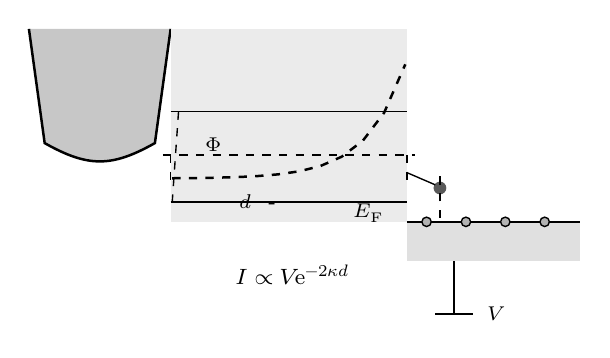
\begin{tikzpicture}[
  x=1cm, y=1cm,
  axisln/.style={thinline, black},
  guide/.style={thinline, black, dashed},
  ann/.style={font=\fontsize{7.2}{8.6}\selectfont, align=center},
  annl/.style={ann, align=left},
  fml/.style={font=\fontsize{8}{10}\selectfont}
]
% ---------- 样品 ----------
\fill[black!12] (6.0,0.05) rectangle (8.2,0.55);
\draw[mainline] (6.0,0.55) -- (8.2,0.55);
\foreach \xx in {6.25,6.75,7.25,7.75} {
  \fill[black!30] (\xx,0.55) circle (1.7pt);
  \draw[thinline] (\xx,0.55) circle (1.7pt);
}
\node[ann] at (7.1,-0.10) {样品};
% ---------- 吸附质 ----------
\fill[black!65] (6.42,0.98) circle (2.3pt);
\node[ann] at (5.55,1.30) {吸附质};
\draw[thinline] (5.85,1.24) -- (6.36,1.02);
\draw[guide] (6.42,0.60) -- (6.42,1.16);
% ---------- 针尖 ----------
\fill[black!22]
  (1.20,3.00) -- (1.40,1.55) .. controls (1.95,1.24) and (2.25,1.24) ..
  (2.80,1.55) -- (3.00,3.00) -- cycle;
\draw[mainline]
  (1.20,3.00) -- (1.40,1.55) .. controls (1.95,1.24) and (2.25,1.24) ..
  (2.80,1.55) -- (3.00,3.00);
\node[ann] at (2.10,2.62) {金属针尖};
% ---------- 势垒区 ----------
\fill[black!8] (3.00,0.55) rectangle (6.00,3.00);
% 【重叠修正，2026-09-30】`势垒区（真空）` 原用 anchor=north west 挂在 (3.08,2.12)，
% 两行基线在 1.91 / 1.60 cm，而 `功函数 $\Phi$` 挂在 (3.32,1.60)（anchor=west，
% 两行基线 1.69 / 1.38），实测前者第二行与后者第一行只差 0.09 cm——
% 7 对字形墨迹相交（最大 `功`×`垒` 0.543 pt²）。改挂势垒区右上角 anchor=north east。
\node[annl, anchor=north east] at (5.95,2.90) {势垒区\\（真空）};
\draw[axisln] (3.00,1.95) -- (6.00,1.95);
\node[ann, anchor=west] at (6.06,1.95) {真空能级};
\draw[axisln] (3.00,0.80) -- (6.00,0.80);
\node[ann, anchor=west] at (5.20,0.66) {$E_{\mathrm{F}}$};
\draw[guide] (3.10,1.95) -- (3.02,0.80);
\node[ann, align=left, anchor=west] at (3.32,1.60) {功函数\\ $\Phi$};
% ---------- 波函数在势垒中的衰减 ----------
\draw[mainline, dashed]
  plot[domain=3.02:5.98, samples=12, variable=\t]
  ({\t},{1.10+1.45*exp(-2.05*(5.98-\t))});
\node[ann, align=left, anchor=west] at (3.10,2.52)
  {电子波函数\\ 向真空衰减};
\node[fml] at (4.55,-0.12) {$I\propto V\mathrm{e}^{-2\kappa d}$};
% ---------- 间距标注 ----------
\draw[guide] (2.90,1.40) -- (6.10,1.40);
\draw[guide] (3.00,1.40) -- (3.00,1.02);
\draw[guide] (6.00,1.40) -- (6.00,1.02);
% 【重叠修正，2026-09-30】`$d$：针尖-样品间距` 原居中挂在 (4.50,1.02)，右端伸到
% x≈5.36 cm，压住 $E_{\mathrm{F}}$（挂在 5.20）：实测 `距`×`E` 墨迹相交 4.6×2.9 pt、
% 轮廓交叠 0.883 pt²。左移 0.25 cm，右端止于 5.11 cm，与 E 标签留 0.09 cm。
\node[ann, anchor=north] at (4.25,1.02) {$d$：针尖-样品间距};
% ---------- 样品偏压 ----------
\draw[axisln] (6.60,0.05) -- (6.60,-0.62);
\draw[axisln] (6.36,-0.62) -- (6.84,-0.62);
\node[ann, anchor=west] at (6.90,-0.62) {$V$};
\end{tikzpicture}
\caption{针尖-样品隧穿结与势垒的能级示意。读者应看两处：电子波函数在势垒区
中的指数衰减、功函数 $\Phi$ 决定的势垒高度（$E_{\mathrm{F}}=-\Phi$）。恒流反馈
回路（隧道电流放大器 $\to$ 反馈控制 $\to z$ 压电元件）与偏压下的能级对齐过程
见正文 §12.1.1--§12.1.2，本图只画隧穿结。图中横向尺寸与实际比例不符，为示意
画法。\schemamark\figsrc{据 S2（下册）图 12-2，书内 p.889—890 / PDF p.375—376 改绘。}}
\label{fig:stm-junction}
\end{figure}

\subsubsection{隧穿电流}

在解释图像衬度起源前，先要理解针尖与表面之间的电子流动过程\src{S2 §12.1.2，
书内 p.889—892 / PDF p.375—378}。两个金属电极靠近但未连通时，真空能级一致、各自费米
能级保持本征值，其差（接触电势）等于两金属功函数之差；用导线连通后真空能级发生偏移、
两者费米能级拉平，真空中出现电场，但费米能级齐平、没有可用能量窗口，故无净电流。只有
引入偏压才能打开能量窗口：被施加正偏压的一侧费米能级相对拉低 $eU$，其最高占据态与另一侧
的未占据态在能量上对齐，电子才发生隧穿；偏压反向则隧穿方向反转。两极相距较远时电流无法
穿越真空势垒，充分接近至 \qty{1}{nm} 左右时两侧电子波函数发生重叠，即出现隧穿电流。

\begin{principle}
取真空能级为能量参考点，金属表面功函数为 $\Phi$，则 $E_{\mathrm{F}}=-\Phi$。在针尖与
样品功函数相同的简化情形下，处于 $E_{\mathrm{F}}-eU$ 与 $E_{\mathrm{F}}$ 之间、能量为
$E_n$ 的样品态 $\varphi_n$ 有机会隧穿入针尖。当偏压远小于功函数值（$eU\ll\Phi$）时，
对电流有贡献的样品态主要位于费米能级附近，电子的隧穿可用恒定势垒下的薛定谔方程描述，
经典禁阻区内 $z$ 点附近的电子波函数为

\begin{equation}
\varphi(z)=\varphi(0)\,\mathrm{e}^{-\kappa z},
\qquad
\kappa=\frac{\sqrt{2m\Phi}}{\hbar}
\label{eq:kappa}
\end{equation}

式中 $\kappa$ 称衰减常数，$\varphi(0)$ 为样品表面处的电子态。于是第 $n$ 个样品态中的
电子出现在针尖表面处（$z=W$）的概率正比于
$\lvert\varphi_n(0)\rvert^{2}\mathrm{e}^{-2\kappa W}$。把能量窗口 $eU$ 内的所有样品态
都包括在内，隧穿电流为

\begin{equation}
I\;\propto\!\!\sum_{E_n=E_{\mathrm{F}}-eU}^{E_{\mathrm{F}}}
\lvert\varphi_n(0)\rvert^{2}\mathrm{e}^{-2\kappa W}.
\label{eq:sumI}
\end{equation}

按局域态密度（local density of states，LDOS）的定义，式~\eqref{eq:sumI} 可改写为

\begin{equation}
\begin{split}
I\;&\propto\;U\,\rho_{\mathrm{s}}(0,E_{\mathrm{F}})\,\mathrm{e}^{-2\kappa W}\\
   &\approx\;U\,\rho_{\mathrm{s}}(0,E_{\mathrm{F}})\,
   \mathrm{e}^{-1.025\sqrt{\Phi}\,W},
\end{split}
\label{eq:tunneling}
\end{equation}

其中 $\rho_{\mathrm{s}}(0,E_{\mathrm{F}})$ 为费米能级附近的表面局域态密度。注意
式~\eqref{eq:tunneling} 的指数上是 $2\kappa W$，故有实用单位定值的是 $2\kappa$ 而不是
$\kappa$：取 $m=\qty{9.109e-31}{kg}$、$\hbar=\qty{1.055e-34}{J.s}$，以 \unit{eV} 表示
$\Phi$、以 \unit{\angstrom} 表示 $W$，则
$2\kappa\approx\qty{1.025}{\per\angstrom}\times\sqrt{\Phi/\unit{eV}}$，即
$\kappa\approx\qty{0.512}{\per\angstrom}\times\sqrt{\Phi/\unit{eV}}$。系数归属已对照
原页面图像核对：原书该步印
$I\propto U\rho_{\mathrm{s}}(0,E_{\mathrm{F}})\mathrm{e}^{-2kW}
\approx U\rho_{\mathrm{s}}(0,E_{\mathrm{F}})\mathrm{e}^{-1.0252\sqrt{\varphi}W}$
（原书把这一衰减常数记作 $k$，本节记作 $\kappa$），$1.0252$ 确实位于整个指数上，即属于
$2\kappa$；本节按所列常数算得 $2\kappa\approx1.024$，与原书末位之差属常数取值与取位，
正文取 $1.025$ \src{S2 §12.1.2，书内 p.891 / PDF p.377}。
\end{principle}

式~\eqref{eq:tunneling} 给出两个必须分开记住的结论。

\textbf{（1）电流对间距指数敏感，带来原子级垂直分辨。} 取 $\Phi=\qty{4}{eV}$，由
式~\eqref{eq:kappa} 得 $\kappa\approx\qty{1.02}{\per\angstrom}$，即指数上的
$2\kappa\approx\qty{2.05}{\per\angstrom}$。这就是本书所说的\textbf{针尖与样品间距每增加
\qty{1}{\angstrom}，隧穿电流约衰减至 $\mathrm{e}^{-2}$（约 $1/7.4$）}；反过来，间距变化
\qty{0.1}{\angstrom} 对应约 23\% 的电流变化。若电流测量精度为 1\%，对应间距变化
$\Delta d=\ln(1.01)/(2\kappa)\approx0.0049$ \AA$\,=\qty{0.49}{pm}$，这正是 STM 纵向
灵敏度可达皮米量级的原因。
但\textbf{灵敏度不等于图像的实际纵向分辨率}：后者还受反馈环带宽、压电陶瓷迟滞与蠕变、
电子学噪声限制，恒流模式 $z$ 通道的实用分辨率通常在 \qtyrange{0.01}{0.1}{\angstrom} 量级。

\textbf{（2）测到的是电子态密度，不是纯几何高度。} 电流正比于
$\rho_{\mathrm{s}}(0,E_{\mathrm{F}})$，即能量窗口内样品表面电子态的数目，而非表面原子的
几何位置。被测的是哪批电子态由偏压极性决定：样品加正偏压时电子由针尖占据态流向样品空态，
探测 $E_{\mathrm{F}}$ 以上的未占据态；样品加负偏压时探测 $E_{\mathrm{F}}$ 以下的占据态。
因此调节偏压即可探测费米面附近不同的态密度，\textbf{同一表面在不同偏压下会给出不同的
像}。

这解释了一个看似矛盾的现象：Xe 吸附于 Ni(110) 时，吸附原子的电子态并不位于费米能级
附近，STM 却仍能很好地成像。原因是 Xe 显著改变了 Ni 的局域态密度——相比真空，Xe 降低了
局域的隧穿势垒，使表面波函数可以进一步延伸到真空中，从而被针尖在更远处探测到
\src{S2 §12.1.2，书内 p.891—892 / PDF p.377—378}。可见图像衬度取决于针尖与样品电子
结构的卷积以及两者间距：洁净金属表面上位置较高的原子通常对应凸起亮点，但对吸附质而言，
衬度还取决于其与基底的相互作用强度、偏压极性与大小、势垒高度的局域变化。相互作用较弱、
不显著改变表面电子结构的吸附物种仍可能被分辨出几何形态，但其表观高度不等于几何高度。

\begin{pitfall}
不要把 STM 图像当等高线图读。同一表面在不同偏压下会得到不同的像，一张像只对应一个能量
窗口内的电子态分布；把表观高度直接当作原子几何高度，是最常见也最难自查的误读。
\end{pitfall}

\subsubsection{恒高模式与恒流模式}

STM 成像有两种主要模式\src{S2 §12.1.1，书内 p.888 / PDF p.374}：\textbf{恒定电流模式}
对压电陶瓷扫描头施加反馈以保持隧穿电流恒定，同时记录为维持恒流所调整的 $z$ 位移随 $xy$
的变化；\textbf{恒定高度模式}保持针尖高度不变，直接测量隧穿电流随 $xy$ 的变化。两者的
差别不只是记录 $z$ 还是记录 $I$，而是\textbf{把指数敏感的那一端接在反馈环上，还是直接
送到信号通道}。

\begin{figure}[htbp]
\centering
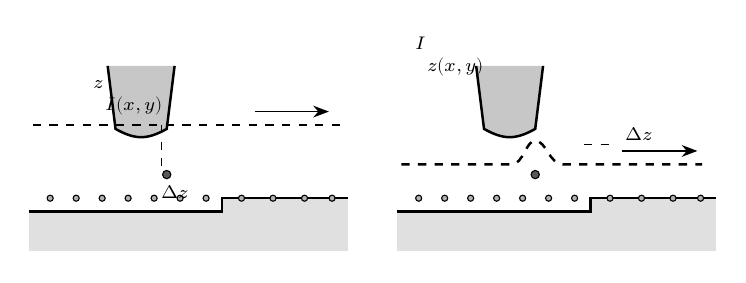
\begin{tikzpicture}[
  x=1cm, y=1cm,
  base/.style={fill=black!12, draw=none},
  surf/.style={mainline},
  atom/.style={fill=black!30, draw=black, line width=0.4pt},
  ads/.style={fill=black!65, draw=black, line width=0.4pt},
  guide/.style={thinline, black, dashed},
  path/.style={mainline, black, dashed},
  ann/.style={font=\fontsize{6.6}{8}\selectfont, align=center},
  annl/.style={ann, align=left}
]
% ================= (a) 恒高模式 =================
\begin{scope}[shift={(0,0)}]
  \fill[base] (0.35,-0.05) rectangle (2.80,0.45);
  \fill[base] (2.80,-0.05) rectangle (4.40,0.62);
  \draw[surf] (0.35,0.45) -- (2.80,0.45) -- (2.80,0.62) -- (4.40,0.62);
  \foreach \xx in {0.62,0.95,1.28,1.61,1.94,2.27,2.60,3.05,3.45,3.85,4.20} {
    \fill[atom] (\xx,0.62) circle (1.1pt);
  }
  \fill[ads] (2.10,0.92) circle (1.5pt);
  \draw[thinline] (2.80,0.62) -- (2.80,0.45);
  \node[ann, align=left, anchor=west] at (2.62,0.02) {台阶};
  \fill[black!22] (1.35,2.30) -- (1.45,1.50) .. controls (1.70,1.36) and
                   (1.85,1.36) .. (2.10,1.50) -- (2.20,2.30) -- cycle;
  \draw[mainline] (1.35,2.30) -- (1.45,1.50) .. controls (1.70,1.36) and
                  (1.85,1.36) .. (2.10,1.50) -- (2.20,2.30);
  \draw[path] (0.40,1.55) -- (4.35,1.55);
  \draw[-{Stealth[length=2mm]}, thinline] (3.22,1.72) -- (4.16,1.72);
  \node[ann, anchor=south] at (3.88,1.76) {扫描方向};
  \draw[guide] (2.03,1.55) -- (2.03,0.99);
  \node[ann, align=left, anchor=west] at (1.05,1.90) {$z$ 预设恒定；\\ 读 $I(x,y)$};
  \node[ann, anchor=north] at (2.20,0.90) {$\Delta z$};
\end{scope}
% ================= (b) 恒流模式 =================
\begin{scope}[shift={(4.68,0)}]
  \fill[base] (0.35,-0.05) rectangle (2.80,0.45);
  \fill[base] (2.80,-0.05) rectangle (4.40,0.62);
  \draw[surf] (0.35,0.45) -- (2.80,0.45) -- (2.80,0.62) -- (4.40,0.62);
  \foreach \xx in {0.62,0.95,1.28,1.61,1.94,2.27,2.60,3.05,3.45,3.85,4.20} {
    \fill[atom] (\xx,0.62) circle (1.1pt);
  }
  \fill[ads] (2.10,0.92) circle (1.5pt);
  \draw[thinline] (2.80,0.62) -- (2.80,0.45);
  \fill[black!22] (1.35,2.30) -- (1.45,1.50) .. controls (1.70,1.36) and
                   (1.85,1.36) .. (2.10,1.50) -- (2.20,2.30) -- cycle;
  \draw[mainline] (1.35,2.30) -- (1.45,1.50) .. controls (1.70,1.36) and
                  (1.85,1.36) .. (2.10,1.50) -- (2.20,2.30);
  \draw[path]
    (0.40,1.05) -- (1.80,1.05) .. controls (1.95,1.05) and (1.98,1.35) ..
    (2.10,1.35) .. controls (2.24,1.35) and (2.28,1.05) .. (2.45,1.05) --
    (4.22,1.05);
  \draw[-{Stealth[length=2mm]}, thinline] (3.20,1.22) -- (4.16,1.22);
  % 【重叠修正】原为 anchor=south at (3.70,1.26)：文字向上展开到 y≈1.36，
  % 而下一行「Δz 被记录」在 (3.12,1.44) 向西对齐、x 覆盖 3.12—4.11，
  % 两者 x 区间几乎完全重合 —— 实测 p.114 出现「扫/Δ」「描/z」两对字符叠印。
  % 改为放到箭头下方（anchor=north），把上方让给 Δz 标注。
  \node[ann, anchor=north] at (3.70,1.16) {扫描方向};
  \node[ann, align=left, anchor=west] at (0.45,2.42) {$I$ 恒定；\\ 读 $z(x,y)$};
  \draw[guide] (2.72,1.30) -- (3.12,1.30);
  \node[ann, anchor=west] at (3.12,1.44) {$\Delta z$ 被记录};
\end{scope}
\end{tikzpicture}
\caption{恒高模式（a）与恒流模式（b）的原理对比。读者应看两点：针尖轨迹的高度是预设的
还是由反馈跟随表面决定的；信号通道记录的是电流还是 $z$ 位移。图中表面起伏与吸附质尺寸
为示意画法，未按真实比例。\schemamark\figsrc{据 S2（下册）§12.1.1 正文
（书内 p.888 / PDF p.374）重绘。}}
\label{fig:stm-modes}
\end{figure}

\begin{measure}
恒流模式的反馈环要求足够的响应速度：扫描越快、表面起伏越陡，环的滞后越明显，针尖轨迹会
削峰填谷，把形貌信息混入电子结构信息。恒高模式没有反馈环，扫描速率只受数据采集与前级
放大器带宽限制，但针尖与样品的最小间距在扫描区内无法自适应，因此要求该区粗糙度远小于
预设间距，偏压与电流设定值也须更保守以避免碰撞\src{S2 §12.1.1，书内 p.888 /
PDF p.374；设定值取舍为据原理的推断}。两者的适用场合不同：恒高模式不必等待反馈稳定，
常用于平整表面的原子分辨成像与快速扫描；恒流模式能安全跨越台阶与纳米颗粒，是粗糙表面、
原位与变温实验的默认选择。正因反馈电路与针尖稳定性的限制，目前的 STM 研究较多集中于
平整表面，以获得原子尺度的空间分辨成像\src{S2 引言，书内 p.887 / PDF p.373}。
\end{measure}

\subsubsection{扫描隧道谱（STS）}

STM 的能力不止于形貌。式~\eqref{eq:tunneling} 已表明图像不仅取决于表面形貌，也取决于加在
针尖上的电压——对电压的控制决定了哪个电子态发生隧穿。因此 STM 可用于原子尺度的局域电子
结构测量，这种数据采集模式称为扫描隧道谱（scanning tunneling spectroscopy，STS）
\src{S2 §12.1.3，书内 p.892 / PDF p.378}。

\begin{principle}
按 WKB 近似，隧穿电流可写成显式积分形式：
\begin{equation}
I\;\propto\!\int_{0}^{eU}\!
\rho_{\mathrm{s}}(\mathbf{r},E)\,
\rho_{\mathrm{t}}(\mathbf{r},\pm eU\mp E)\,
T(E,eU,\mathbf{r})\,\mathrm{d}E ,
\label{eq:wkb}
\end{equation}
式中 $\rho_{\mathrm{s}}(\mathbf{r},E)$ 与 $\rho_{\mathrm{t}}(\mathbf{r},E)$ 分别为样品与
针尖在位置 $\mathbf{r}$、能级 $E$ 处的电子态密度；$+eU-E$ 对应样品加正偏压，
$-eU+E$ 对应样品加负偏压；$T$ 为隧穿概率函数。取针尖态密度在讨论的能量范围内近似平坦，
并对偏压求导——低温极限下费米分布的导数趋于 $\delta$ 函数——于是
\begin{equation}
\left.\frac{\mathrm{d}I}{\mathrm{d}V}\right|_{\mathbf{r}}
\;\propto\;\rho_{\mathrm{s}}(\mathbf{r},E_{\mathrm{F}}+eV)\;
T(E_{\mathrm{F}},eV,\mathbf{r}).
\label{eq:dIdV}
\end{equation}
即\textbf{微分电导正比于针尖所在位置的样品局域态密度}。这就是 STS 测的是电子结构而非
形貌的原因：式~\eqref{eq:dIdV} 的右端只含态密度与隧穿概率，几何高度没有独立地位。
式~\eqref{eq:wkb} 的积分限与能量宗量已逐字核对：原书印
$I=\int_{0}^{eU}\rho_{\mathrm{s}}(r,E)\rho_{\mathrm{t}}(r,\pm eU\mp E)T(E,eU,r)\mathrm{d}E$，
并写明「$+eU-E$ 对应对样品施加正偏压 $eU$ 的情况；$-eU+E$ 对应于对样品施加负偏压 $eU$
的情况」（原书用等号，本节省去前置常数故写正比号）。原书紧接的一句是「归一化后的微分电导
将只取决于局域态密度和隧穿电压」，确以 $I/V$ 归一化为前提；式~\eqref{eq:dIdV} 是本节据该
表述补出的求导形式，原书未列出式~\eqref{eq:dIdV}。
\src{S2 §12.1.3，书内 p.892 / PDF p.378，STS 一节的隧穿电流积分式}
\end{principle}

\begin{dataflow}
STS 的数据链条是：针尖固定在 $\mathbf{r}$ 处扫偏压得到 $I(V)$ 曲线（非线性）$\rightarrow$
取微分电导 $\mathrm{d}I/\mathrm{d}V$ $\rightarrow$ 按式~\eqref{eq:dIdV} 换算为费米能级附近
的局域态密度 $\rho_{\mathrm{s}}(\mathbf{r},E_{\mathrm{F}}+eV)$ $\rightarrow$ 在 $xy$ 上
逐点重复得到 LDOS 空间成像。实际操作中常在直流偏压上叠加小幅高频调制，用锁相放大器取
电流的一阶谐波直接得到 $\mathrm{d}I/\mathrm{d}V$（这是 STS 的通行做法，非本书记载）。
STS 之所以必要，是因为它能把几何上相似的对象分开：氧化物表面的桥氧空位与轻原子吸附物种
在形貌图上可能都表现为亮点，而同一次实验采集的 $\mathrm{d}I/\mathrm{d}V$ 曲线或映射图可按
电子结构把它们分辨开；反过来，表观高度不同的两个物种在 STS 上也可能给出相同的谱，此时
不能据形貌图推断活性位不同。
\end{dataflow}

STS 在纳米催化中的一个典型用法是测量局域功函数与局域态密度随结构参数的变化，见
\ref{sec:model-nano} 节。六环节在本节的落点是：\textbf{问题与输出}确定 STM 给出 $I(x,y)$
或 $z(x,y)$；\textbf{原理与公式}（式~\eqref{eq:tunneling}）说明电流为何对间距指数敏感、
又为何编码态密度；\textbf{测量与条件}给出恒高与恒流模式的取舍；\textbf{数据到结论}把
$z$ 通道换算为形貌、把 $\mathrm{d}I/\mathrm{d}V$ 换算为局域态密度；\textbf{误判与边界}
与\textbf{互补与回查}分别见后两节。

\subsection{STM 在催化研究中的应用}

\subsubsection{催化反应机理和动力学的可视化研究}

随着低温和变温 STM 技术的发展，STM 可以实时监测化学反应，即反应物的化学吸附、扩散和催化
转化的基元步骤\src{S2 §12.2.1，书内 p.892—903 / PDF p.378—389}。低温下表面扩散被抑制、
吸附物种的运动完全可控，有利于中间体鉴定；STM 还可用针尖脉冲诱发吸附、脱附与解离。在
Ag(110) 上，针尖在分子氧顶端施加 \qty{0.47}{V} 脉冲使其解离为一对氧原子，\qty{0.24}{V}
脉冲可驱动 CO 迁移；CO 靠近氧原子对时自动形成 O—CO—O 复合体，复合体在脉冲下解离，
生成的 \ce{CO2} 脱附而表面留下一个氧原子，全程遵循 Langmuir--Hinshelwood 机制。针尖操纵
与成像结合，说明 STM 能在单分子水平做反应路径成像。

\textbf{从扩散看活性位。} 覆盖度增加时吸附分子间的相互吸引导致吸附质岛形成，并与自由移动
的分子保持动态平衡。跟踪表面空位扩散可得到活性位信息：在约 \qty{65}{K} 与
\qty{2e-7}{torr}（\qty{1}{torr}=\qty{133.32}{Pa}）的 \ce{H2} 中 Pd(111) 表面可被 H 饱和，
由于针尖吸附了 H 原子，成像机制反转，\textbf{吸附空位表现为凸起亮点}。连续图像显示空位
二聚体会重新解离为孤立空位，而\textbf{三聚体消失只留下一个空位}，说明其中两个空位被
\ce{H2} 解离产生的两个 H 占据；大量统计表明只有三个或更多空位的聚集体才会被 H 占据，即
\ce{H2} 在 Pd 表面的解离需要三个或更多紧邻空位\src{S2 §12.2.1，书内 p.894—895 /
PDF p.380—381}——这与「两个相邻空位已足够」的传统默认不同。

\textbf{氧化物表面。} 金红石 \ce{TiO2}(110) 表面桥氧加热时部分脱附形成桥氧空位，这是该表面
最常见的缺陷位。结合原位 STM 与 DFT 可把活性位、吸附物种与中间体区分开：常用正偏压扫描下
5 配位 Ti 原子列成像为亮行、桥氧列成像为暗行，桥氧空位、表面 OH 与吸附 \ce{H2O} 有明显
的表观高度差异。由此得到：\ce{H2O} 优先在桥氧空位吸附解离，解离的 H 落到近邻桥氧上形成
配对 OH；测量 300—\qty{410}{K} 的迁移速率得，相邻桥氧位上的 H（$H_{\mathrm{B}}$）的迁移
能垒比空位 OH 上的 H（$H_{\mathrm{V}}$）低约 \qty{0.22}{eV}，且能垒随 OH 间距增大而增加，
表明 OH—OH 排斥帮助了 H 的迁移；甲醇在桥氧空位解离吸附形成的甲氧基比桥氧空位高
\qty{0.8}{\angstrom}，随后 OH 中 H 的迁移可被逐帧跟踪\src{S2 §12.2.1，书内 p.895—899 /
PDF p.381—385}。

\textbf{反应机理。} 第 \textsc{viii} 族贵金属催化的氢氧化反应是 1823 年发现的第一个催化
反应，其机理长期不清楚：通常认为经 \ce{O_{ad}} 与 \ce{H_{ad}} 结合成羟基、再与另一个
\ce{H_{ad}} 成水，羟基形成常被假定为决速步，但羟基难以在早期光谱研究中证实。在
\ce{Pt}(111) 上预吸附 \ce{O2} 形成 $(2\times2)$--\ce{O_{ad}}（\ce{O_{ad}} 为暗点）后通入
\ce{H2}：上方出现亮岛并扩大，最终形成氢键连接的 \ce{OH_{ad}} 有序覆盖层，图像中还可见
迁移的小团簇（\ce{H2O_{ad}}）。大尺度上可见随时间向外扩展的亮环，即\textbf{反应前沿}：
边界处 \ce{O_{ad}} 与扩散 \ce{H2O_{ad}} 快速反应生成两个 \ce{OH_{ad}}，后者再与
\ce{H_{ad}} 快速成水。由于 \ce{O_{ad}}+\ce{H_{ad}} 成羟基是决速步，\ce{H2O_{ad}} 的参与
消除了这一限制，形成\textbf{自催化}过程，这解释了氢氧化在水的脱附温度以下仍有高活性的
来源；当 \ce{H2O} 开始脱附、\ce{H2O_{ad}} 寿命缩短，自催化循环即被打破
\src{S2 §12.2.1，书内 p.900—901 / PDF p.386—387}。

\begin{dataflow}
\textbf{反应动力学。} 单晶表面 CO 氧化的原位 STM 研究通常用\textbf{滴定实验}：预吸附
\ce{O_{ad}} 后暴露于恒定压力的 CO，速率直接由覆盖度随时间的变化得到。在 \ce{Pt}(111) 上，
\qty{247}{K} 下 \ce{O_{ad}} 形成有序 $(2\times2)$--O（暗点）；通入 \qty{5e-8}{torr} CO 后
CO 形成 $c(4\times2)$ 并扩大，$(2\times2)$--O 岛面积减小。把面积减小速率对周长（两类区域
的畴界长度）与对 $\theta_{\mathrm{O}}(1-\theta_{\mathrm{O}})$ 分别作图，可见\textbf{速率
与周长线性相关}，说明 CO 氧化主要沿边界发生；在 237—\qty{274}{K} 重复滴定，求得活化能约
\qty{0.49}{eV}、指前因子约 \qty{3e21}{cm^{-2}.s^{-1}}，与宏观测量相符
\src{S2 §12.2.1，书内 p.901—903 / PDF p.387—389}。并非所有体系都能用简单级数描述：
\ce{Ag}(110) 上 \ce{O2} 解离引起的 $(n\times1)$--O 重构由一维 AgO 链构成，室温暴露于
\qty{1e-8}{torr} CO 时链分段消失、速率显著加快；低于 \qty{230}{K} 时反应只发生在链末端，
为零级动力学，能垒约 \qty{41}{kJ/mol}。
\end{dataflow}
\subsubsection{近常压 STM 研究}

上节的研究暴露出一个根本疑虑：化学吸附可改变催化剂表面结构或组分，超高真空下的结果能否
外推？此前表征常在 \qtyrange{1e-14}{1e-10}{bar} 的 UHV 下进行，而工业催化在
\qtyrange{1}{1000}{bar} 下进行，超过十个数量级的压差可极大改变反应物在表面的相互作用。
要跨越这一\textbf{压力鸿沟}，原位 STM 的观测必须拓展到近常压甚至高压
\src{S2 §12.2.2，书内 p.903—904 / PDF p.389—390}。Salmeron 等较早把常压 STM 用于模型
催化剂，展示了 \ce{Pt}(110) 在接近一个大气压的 \ce{H2}、\ce{O2} 或 CO 中的重构。Frenken
等进一步把扫描头置于流动反应器内：UHV 中 \ce{Pt}(110) 重构为 $(1\times2)$，CO 可消除该
重构；在 \qty{1}{bar} CO 下高压 CO 不仅消除重构还使表面粗糙化——\qty{425}{K}、
\qty{1.25}{bar} CO 下由 $(1\times2)$ 向 $(1\times1)$ 的重排导致表面碎片化并形成高密度
台阶（$t=0$ min 呈虎皮状），随后台阶熟化、表面平滑并形成 CO 覆盖的大岛。

把 CO/\ce{O2} 混合气通入反应器，同时用四极质谱仪实时监测 CO、\ce{O2} 与 \ce{CO2}，即可
实现表面结构与反应性能的同时测量，即 \textbf{operando} STM。按速率可分为两阶段：低活性
阶段图像无明显变化，Pt 保持金属态；高活性阶段速率约为前者的 3 倍，表面粗糙、可能有铂
氧化物形成，且粗糙度随速率均匀增加。结合高压 SXRD（该相被指认为铂氧化物单层）与动力学
测量，Frenken 等提出高活性阶段 CO 可直接与表面氧化物的氧反应，即 Mars--van Krevelen
机制；但书中明确指出，由于高压环境的复杂性（如气体输运受限时表面附近气相可与远处气相
大不相同），该构效关系仍存争议，还需结合谱学做更多 operando 研究
\src{S2 §12.2.2，书内 p.905—906 / PDF p.391—392}。高压 STM 的必要性正在于此：高压气体
造成的吸附物种结构常可在高真空低温实验中重现，但金属原子在低温下运动受限，表面结构在
实际催化条件下的\textbf{动态}变化难以在 UHV 中直接观察。
\subsubsection{负载型纳米结构催化剂的模型研究}
\label{sec:model-nano}

实际催化剂常由 \qtyrange{1}{10}{nm} 的活性纳米颗粒分散在高比表面载体上构成，颗粒可具有与
体相完全不同的结构和性质，由此产生与单晶平整表面之间的\textbf{材料鸿沟}。反应性和选择性
常取决于颗粒的大小、形貌及与载体的相互作用，即\textbf{尺寸效应}与\textbf{界面效应}，而
这两个效应无法从平整单晶表面的研究得到\src{S2 §12.2.3，书内 p.907 / PDF p.393}。

\textbf{金属-氧化物界面位点。} 包信和团队在 \ce{Pt}(111) 表面构筑 FeO--Pt 界面位点，发现
Pt 表面可稳定配位不饱和的 \ce{Fe^{2+}}（coordinatively unsaturated ferrous，CUF）中心；
该位点在室温 Pt 表面被 CO 毒化时仍保持很高的 \ce{O2} 活化能力，可实现富氢条件下 CO 的
选择性氧化（PROX）。进一步构筑不同尺寸的 FeO 纳米三角形岛后，由 STM 图定出各岛的化学
计量比（如 \ce{Fe66O55}、\ce{Fe190O171}、\ce{Fe378O351}），边界均呈现相同的 CUF 结构。
STS 结果显示：局域功函数（local work function，LWF）与局域态密度（LDOS）随 FeO 在
\ce{Pt}(111) 上的\textbf{落位}而变——Fe 落在 fcc 位点时 LWF 最大（\qty{5.1}{eV}），落在
top 位点时最低（\qty{4.2}{eV}）；但边长 $>\qty{3}{nm}$ 的不同尺寸纳米岛在相同落位（即
相同 Pt--Fe--O 界面结构）表现出相同的 LWF 与 LDOS，不受尺寸影响。LDOS 空间成像还显示，
边界靠近 top 位点及 top-FeO 区域在费米能级以上约 \qty{0.5}{eV} 处呈共振峰
\src{S2 §12.2.3，书内 p.907—908 / PDF p.393—394}。

这里出现一个值得记录的反差。传统认识上相同的活性结构与电子结构必然带来相同的活性，但用
原位 STM 观察不同尺寸 FeO 纳米岛与 \ce{O2} 的相互作用时，\ce{O2} 在 CUF 边界的吸附解离
同时带来岛的\textbf{动态重构}，且明显依赖尺寸：边长约 \qty{3}{nm} 的岛在氧解离后整个岛面
Fe--O 位置相对偏移，最终整个岛的氧晶格重构为稳定的二配位氧终止边；而边长大于
\qty{4}{nm} 的岛只能部分重构，未重构的 CUF 边界吸附了相对不稳定的氧原子，岛面出现重构区
与未重构区之间的畴界。这种与尺寸相关的氧气氛动态重构被称为\textbf{动态尺寸效应}，显著
影响 FeO 纳米粒子在 \ce{O2} 中的稳定性：在 \qty{500}{K}、\qty{1e-5}{mbar} \ce{O2} 中处
理时，尺寸小于 \qty{3.2}{nm} 的岛因更易完整重构、边界形成惰性的二配位氧终止边而表现出
反常的抗氧化行为，大岛则因重构不完全、边界存留的不稳定氧较易从 CUF 边或畴界扩散进入而
深度氧化\src{S2 §12.2.3，书内 p.908—910 / PDF p.394—396}。

\begin{infer}
上例说明：STS 显示的「电子结构不随尺寸变化」与原位 STM 显示的「反应行为随尺寸变化」并不
矛盾——前者描述反应前特定落位上的电子结构，后者描述\textbf{吸附诱导重构后}的终态。若只用
STS 或形貌图之一推断活性，会把反应过程中的结构演化漏掉。
\end{infer}

STM 也能解析实际纳米催化剂结构。Goodman 等在 Mo(112) 上预制备 \ce{SiO2} 单层薄膜，把分子
团簇催化剂 \ce{Ru3(CO)9(SnPh2)3}（Ph 为苯基）经溶液分散沉积到膜上并在真空中加热去除 CO
与苯基配体；高分辨 STM 图显示其原子分辨图包含\textbf{六个金属原子}，排列与前体团簇中的
\ce{Ru3Sn3} 相同，表明配体低温去除时团簇骨架在氧化硅表面保持完整
\src{S2 §12.2.3，书内 p.910 / PDF p.396}。

\textbf{金属载体强相互作用（SMSI）。} 20 世纪 70 年代 Tauster 等发现第 \textsc{viii} 族
过渡金属（如 Pt、Ir）负载在 \ce{TiO2} 上并在较高温度还原时表现出不寻常特性（对 CO 和
\ce{H2} 的化学吸附受抑制而甲烷化活性增加），据此提出 SMSI 概念，其起源至今仍是热点。
Bowker 等把平均约 \qty{4}{nm} 的 Pd 颗粒负载于 \ce{TiO2}(110)，在 \qty{673}{K}、
\qty{5e-8}{mbar} \ce{O2} 下做原位 STM：\ce{O2} 在 Pd 上的解离效率比在 \ce{TiO2}(110) 上
高 3 个数量级，故解离主要发生在 Pd 上，解离的 O 随即溢流到相邻表面并与扩散到表面的间隙
态 \ce{Ti^{3+}} 结合，使 Pd 周围 \ce{TiOx} 富集；\ce{TiOx} 层再生长加速并最终超过 Pd
颗粒高度将其包裹。原位 STM 因此证实\textbf{氧化物包裹}是 SMSI 的重要原因
\src{S2 §12.2.3，书内 p.910—911 / PDF p.396—397}。

\textbf{Au 纳米颗粒的烧结动力学。} 纳米粒子的烧结有两种传质模式：整个粒子的迁移与团聚，
以及单体（单个金属原子或配合物）的迁移与颗粒熟化（Ostwald 熟化）。Goodman 等在 UHV 与近
常压条件下研究 Au/\ce{TiO2}(110)：真空下 Au 颗粒在室温保持稳定，而引入 \qty{0.1}{torr}
的 CO/\ce{O2} 混合气（$1\!:\!1$）后立刻开始烧结。连续原位 STM 显示粒子\textbf{位置没有
变化}，而小粒子逐渐变小消失、大粒子长大，直接表明发生了 Ostwald 熟化而非粒子迁移；单独
暴露于 \ce{O2} 或 CO 时几乎无变化，故推断是混合气的协同作用诱导并加速了烧结。基于
Ostwald 熟化模型，对直径 \qty{3}{nm} 的 Au 粒子求得表观熟化活化能约 \qty{10}{kJ/mol}，
与该催化剂上 CO 氧化的活化能相近\src{S2 §12.2.3，书内 p.911—912 / PDF p.397—398}。
\subsection{误判与边界}
\label{sec:stm-pitfall}

\subsubsection{针尖卷积与「双针尖」假象}

STM 图像是针尖形状与样品表面电子结构的\textbf{卷积}，不是表面的直接投影。理想针尖末端只有
一个原子突起，实际针尖常有多个突起：每个突起各形成一条隧穿通道，图像便是这几条通道的
叠加，表现为\textbf{重影、孪生特征或特征被复制到邻近位置}，即「双针尖」（double tip）
假象。判据是：重影的出现与消失依赖于针尖处理，改变扫描方向时重影的相对位置发生变化，
同一样品更换针尖后重影消失。针尖卷积还会放大小尺寸特征的表观尺寸、抹圆单原子台阶、使
孤立吸附质的表观高度偏离几何高度，极端情形下把同一吸附质成像两次而使覆盖度被高估。另一
类反转与针尖状态有关：Pd(111) 上吸附了 H 原子的针尖会把\textbf{吸附空位}成像为凸起亮点
\src{S2 §12.2.1，书内 p.894 / PDF p.380}，此时按几何直觉解读会把空位误认为吸附物种、把
空位团簇的消失误认为吸附物种脱附；\ce{TiO2}(110) 上的氧空位同样成亮点是反例。

\begin{pitfall}
凡要从 STM 图读出「有几个原子」「覆盖度是多少」「哪个是吸附质」的结论，都必须先排除针尖
卷积：用不同针尖重复、改变扫描方向、用针尖脉冲处理后再成像，三种办法至少用两种。只凭
一张像下的结论不可靠。
\end{pitfall}

\subsubsection{STM 图像是电子态密度图}

同一表面在改变偏压时会给出不同的像，这是原理决定的，不是仪器故障——原因见
式~\eqref{eq:tunneling} 与式~\eqref{eq:dIdV}：不同偏压对应不同能量窗口。因此「STM 图上的
亮点」必须与偏压一起报告；不同文献中同一体系的表观高度不一致，往往源于偏压符号与数值不同
或针尖末端态密度差异，而不一定是样品不同。由此派生三条常见误读：把表观高度差直接当作
几何高度差；把亮点一律当作位置更高的原子（Pd(111) 的 H 空位、\ce{TiO2}(110) 的空位都是
反例）；把不同偏压下的两张像逐点相减当作同一批原子的位移。

\subsubsection{近常压 STM 中针尖与气体的相互作用}

近常压环境本身会改变测量。针尖在气体中可能被 CO 或其他物种覆盖，改变其电子结构与有效
功函数，甚至如 Pd/H 的例子那样反转成像机制；针尖-样品间隙中的气体分子也可能参与隧穿或
改变势垒高度，使电流-电压关系偏离式~\eqref{eq:tunneling} 的简化形式；高气压下气体输运
受限，表面附近气相成分可与远处气相不同，因此把质谱测得的体相压力直接当作表面反应条件是
不安全的\src{S2 §12.2.2，书内 p.905—906 / PDF p.391—392}。此外，operando 条件下扫描速率
与反应速率可能处于同一时间尺度，图像中看到的「结构」有可能是扫描期间的时平均结果。

\subsubsection{模型体系结论外推的边界}

这一条决定 STM 结果在催化中的适用范围。前述 12.2 的绝大多数结论来自\textbf{超高真空中、
单晶（或单晶上的有序氧化物纳米岛）表面、低温或中等温度}下的模型体系。外推到真实负载型
催化剂时至少有三重边界\src{S2 §12.2.2—12.2.3，书内 p.903—912 / PDF p.389—398}。

\textbf{（1）压力边界。} UHV 表征常在 \qtyrange{1e-14}{1e-10}{bar}，工业催化在
\qtyrange{1}{1000}{bar}，相差十个数量级以上。高压下表面可发生 UHV 中不出现的重构（如
\ce{Pt}(110) 在 \qty{1}{bar} CO 下的粗糙化与台阶熟化）甚至形成新的表面相（高活性阶段的
铂氧化物）。低温高覆盖度实验能复现高压下的吸附结构，却不能复现高压下的表面动力学，因为
金属原子在低温下运动受限。

\textbf{（2）材料边界（材料鸿沟）。} 真实催化剂是 \qtyrange{1}{10}{nm} 的颗粒分散在高比
表面载体上，颗粒有尺寸分布、多种暴露晶面与载体接触界面；模型体系则是大面积单晶平台或
尺寸单一、边界结构统一的有序纳米岛，尺寸效应与界面效应恰好在其中被标准化掉了。FeO 纳米
岛的例子显示了这种标准化的代价：边长大于 \qty{3}{nm} 的岛在相同落位上电子结构相同，但
一旦与 \ce{O2} 作用，重构行为就重新表现出尺寸依赖性，而这个依赖性在静息的电子结构上看
不出来。模型体系的有序度本身也是精心制备的产物，真实载体上的分散状态与之差距很大。

\textbf{（3）方法边界。} STM 只能测导电或半导体样品，只能看到表面最外层的电子态分布，
本身\textbf{不提供化学识别}——区分物种要靠 STS、针尖操纵脱附实验或与谱学手段回查，因此
从 STM 图出发的活性位归属在原理上是间接结论。

综合起来，STM 结论可靠的外推范围是「与模型体系在同量级压力、同量级尺寸、同一表面化学
环境」。跨越压力鸿沟或材料鸿沟的推论必须重新取证：要么在近常压/高压下做 operando 测量，
要么在真实催化剂（或其高分散模型）上重复，要么由谱学与理论计算独立支持。

\subsection{互补与回查}
\label{sec:stm-cross}

形貌图与同一区域的 STS 映射应一起解读：前者给出几何形貌，后者给出费米面附近的局域态密度；
若两者对活性位的归属矛盾，应优先怀疑针尖状态或偏压选择，而不是样品本身。STS 测得的局域
功函数须与独立手段对照——宏观功函数测量、Kelvin 探针、紫外光电子能谱（UPS）给出面平均或
较大面积的平均值，STS 给出单个落位上的值，二者不一致是正常的（前者是平均、后者是分布），
但不能矛盾到量级不符；FeO/\ce{Pt}(111) 上 fcc 落位 \qty{5.1}{eV} 与 top 落位
\qty{4.2}{eV} 的差异需要 DFT 独立支持才能作为「落位决定电子结构」的结论。

动力学参数必须与宏观动力学对照。\ce{Pt}(111) 上 CO 氧化正是一个成功回查：由 STM 滴定求得
的活化能约 \qty{0.49}{eV} 与指前因子约 \qty{3e21}{cm^{-2}.s^{-1}} 与宏观测量相符，这既
验证了 STM 测速的可靠性，也说明由「速率正比于畴界长度」推出的「反应沿边界发生」这一微观
图像是自洽的。高压/operando 结构必须与高压谱学对照：Frenken 等对高活性阶段表面相的归属
依赖高压 SXRD 的独立结果，即便如此书中仍强调该构效关系存在争议，说明\textbf{单一
operando STM 不足以定论}。最后是模型体系与真实催化剂的回查：从单晶或有序纳米岛得到的
尺寸效应、界面效应结论，都应在真实负载催化剂或高分散模型催化剂上检验其边界。

\begin{crosscheck}
STM 提供空间分辨，STS 提供局域电子结构，二者仍不提供化学识别。判断物种归属时至少需要两条
独立证据链：一条来自图像（表观高度、针尖操纵脱附、偏压依赖性），另一条来自谱学或理论
计算。缺少第二条链时，把「亮点」直接命名为某个吸附物种是超出数据支持的推断。
\end{crosscheck}
}{}
\IfFileExists{chapters/parts/ch12-b.tex}{% ================================================================
%  chapters/parts/ch12-b.tex
%  第 12 章  扫描探针显微镜与纳米光谱技术（分片 b）
%  源：S2（下册）第 12 章，书内 p.913—925 / PDF p.399—411
%  范围：12.3（AFM 基本原理：相互作用力、结构与工作模式）、
%        12.4（AFM 数学分析模型）、12.5（AFM 在表面催化相关领域中的应用）
%  不含：12.1—12.2（STM，分片 a）、近场光学 / TERS / Nano-FTIR（分片 c）
%  说明：本分片不写 \chapterstart（分片 a 已写）。
% ================================================================

\subsection{原子力显微镜的基本原理}
\label{sec:afm-principle}

\begin{probout}
原子力显微镜（atomic force microscope，AFM）测量的是\textbf{针尖与样品之间的力}：微悬臂
末端的针尖在样品表面扫描，针尖--样品相互作用力使悬臂发生偏转、或改变其振动状态，检测这
一变化即可反推表面信息。原始输出有三类：$z(x,y)$ 高度像、悬臂振动的振幅/相位（或频移）像，
以及逐点或逐位置的力--距离曲线（力学谱）。它\textbf{不要求样品导电}，因此把原子级表面
成像从金属与半导体扩展到氧化物、分子筛与负载型催化剂；代价是同一幅像里混合了几何形貌、
力学性质与吸附层信息，\textbf{高度不等于几何高度}。
\end{probout}

\subsubsection{与 STM 的根本差别：测力，而不是测电流}

STM 的成像信号是针尖与表面之间的隧穿电流，前提是二者能构成隧穿结：样品必须有一定导电性，
或被减薄到足以导电。这一条把大多数催化剂载体挡在门外——\ce{CeO2}、\ce{TiO2}、\ce{Al2O3}、
分子筛等宽禁带氧化物与绝缘体在常规偏压下给不出稳定的隧穿电流
\src{S2 §12.3，书内 p.913 / PDF p.399}。

AFM 换掉的正是这个前提：它探测针尖尖端原子与样品表面原子之间的\textbf{相互作用力}。
力不需要载流子输运，因此\textbf{导体、半导体与绝缘体一视同仁}——只要针尖能与表面建立
可检测的力，就能成像。这是 AFM 成为氧化物表面结构表征主力工具的原因，也是它在负载型
金属催化剂研究中的立足点：载体是绝缘的，金属纳米粒子长在载体上，只有不依赖导电性的
方法才能在同一次扫描中同时看到二者。反过来，AFM 也因此丢掉了 STM 的一个优势——
STM 电流对局域电子态密度敏感，AFM 的力信号不直接给电子结构，二者互补而非替代
（见 \ref{sec:afm-crosscheck} 段）。

AFM 的技术沿革可以看成一条"把力测得更准"的路线\src{S2 §12.3，书内 p.913 / PDF p.399}：
Binnig 等在早期 STM 实验中注意到针尖与表面之间存在微弱作用力，据此于 1986 年发明第一台
AFM，突破了 STM 对样品导电性的要求；1987 年 Martin 等引入非接触模式，并测量了针尖--样品
不同间距下的力曲线；1991 年基于频率调制的 AFM 问世并成功用于真空中成像；1993 年 Zhong 等
发明轻敲模式，大幅提高成像稳定性，并很快被用于液体中成像；1996 年 Giessibl 把钟表工业
广泛使用的石英音叉（quartz tuning fork）用作 AFM 微悬臂，发明 qPlus 力学传感器，实现
Si(111)-($7\times7$) 表面的原子分辨；2007 年 Custance 等用原子力谱实现合金表面单原子的
元素区分；2009 年 Gross 等用非接触 AFM 实现实空间碳碳化学键的直接观测，把分辨率推进到
亚原子级。目前 AFM 已广泛用于真空、大气与液体中的成像，以及原子操纵和分子识别，其功能
还可扩展到近场光学成像（分片 c）。

\subsubsection{针尖--样品间的相互作用力}

\begin{principle}
AFM 通过探测针尖尖端与样品表面之间的力学信号成像。针尖探测到的总有效相互作用力可取正值
（排斥）或负值（吸引），二者分别定义了排斥与吸引两个成像工作区。总力由几种长程力与短程力
贡献而成：长程力中除静电力外，最常见的是范德华力（van der Waals force），它是吸引性的，
广泛存在于中性原子与分子之间；短程力只在针尖--样品距离很近时才明显，来自针尖尖端原子与
样品表面原子之间的化学成键作用及 Pauli 排斥作用。对不带电的针尖与样品：间距大于
\qty{1}{nm} 时长程范德华作用最大，一般表现为吸引；针尖继续靠近到接近化学成键距离时，
短程吸引性化学力（源于针尖与表面原子最外层电子波函数的交叠）使吸引力达到最大；越过成键
距离后间距继续减小，电子间 Pauli 排斥急剧增加，排斥力占据主导
\src{S2 §12.3.1，书内 p.913--914 / PDF p.399--400}。
\end{principle}

对不带电的针尖与样品，这一距离依赖可以用势能曲线（Lennard-Jones 势）概括：

\begin{equation}\label{eq:lj}
U(d)=4\varepsilon\left[\left(\frac{\sigma}{d}\right)^{12}-\left(\frac{\sigma}{d}\right)^{6}\right]
\end{equation}

式中 $d$ 为针尖--样品间距，$\varepsilon$ 为势阱深度，$\sigma$ 为零势能间距；$d^{-12}$ 项
代表短程 Pauli 排斥，$d^{-6}$ 项代表长程范德华吸引。力为势能的负梯度，
$F_{\mathrm{ts}}=-\dd U/\dd d$。

\tocheck{未对照原页面图像：源书正文只说"势能曲线（Lennard-Jones 势）可以反映针尖--表面
相互作用随间距的变化特点"，未给出解析式；式~\eqref{eq:lj} 按标准 Lennard-Jones 形式补写，
源书对 $\varepsilon$、$\sigma$ 的符号与取值约定未见正文定义。}

源书图 12-21（a）把隧穿电流与针尖--样品作用力随距离的变化画在同一张图上，可直接读出三件事：
隧穿电流随距离减小而单调增加；针尖--样品作用力先由吸引主导并随距离减小而增大到最大吸引，
接近成键距离时排斥力不断增加，以致在总力为零处到达成键距离，成键距离以下则由急剧增加的
排斥作用主导；因此\textbf{若 AFM 能稳定探测短程力，针尖就能在比 STM 更近的距离下操作，
从而获得更好的分辨}\src{S2 §12.3.1，书内 p.914 / PDF p.400}。这句判断值得单独记住：AFM 的
分辨率上限并不来自"力"本身，而来自能否把短程力从长程背景中分离出来——后面三种工作模式的
差别，本质上就是分离方式与工作距离的差别。

\subsubsection{微悬臂探针与偏转检测}

AFM 的主要组成部分与 STM 十分类似：基于压电陶瓷的针尖--样品运动系统、反馈控制电路单元，
以及探针检测系统。AFM 的核心在力学传感器，目前广泛采用的是微悬臂探针
（cantilever--tip）系统：微悬臂前端有突出的针尖，在不同的针尖--样品力学作用下微悬臂发生
相应偏转（deflection），根据偏转程度即可反映表面信息
\src{S2 §12.3.2，书内 p.914 / PDF p.400}。

\begin{measure}
悬臂偏转最常用的检测技术有两类：一是基于光束发射或干涉的\textbf{偏转检测}（光束偏转法），
二是基于压电效应的\textbf{自检测}。光束偏转法把激光聚焦在悬臂背面，反射光落到四象限光电
探测器上，悬臂偏转使光斑在探测器上位移，位移量转成电压信号（图~\ref{fig:afm-setup}）；
它是"光杠杆"，把纳米级的悬臂偏转放大成探测器上毫米级的光斑移动，这是 AFM 能分辨皮米量级
位移的原因。写入正文时真正需要记录的条件只有四组：\textbf{悬臂弹性常数 $k$}（决定同样偏转
对应多大的力，也决定会不会压坏样品）、\textbf{共振频率 $f_0$ 与品质因数 $Q$}（决定动态
模式的振幅稳定性与响应速度）、\textbf{针尖半径 $R$}（决定横向分辨率与卷积加宽，见
\ref{sec:afm-conv} 段）、以及\textbf{环境}（真空/大气/液体，直接决定表面有无吸附水膜）
\src{S2 §12.3.2，书内 p.914--915 / PDF p.400--401}。任何一条没有随图给出，力曲线的定量
结论就不能跨实验比较。
\end{measure}

\begin{figure}[htbp]
\centering
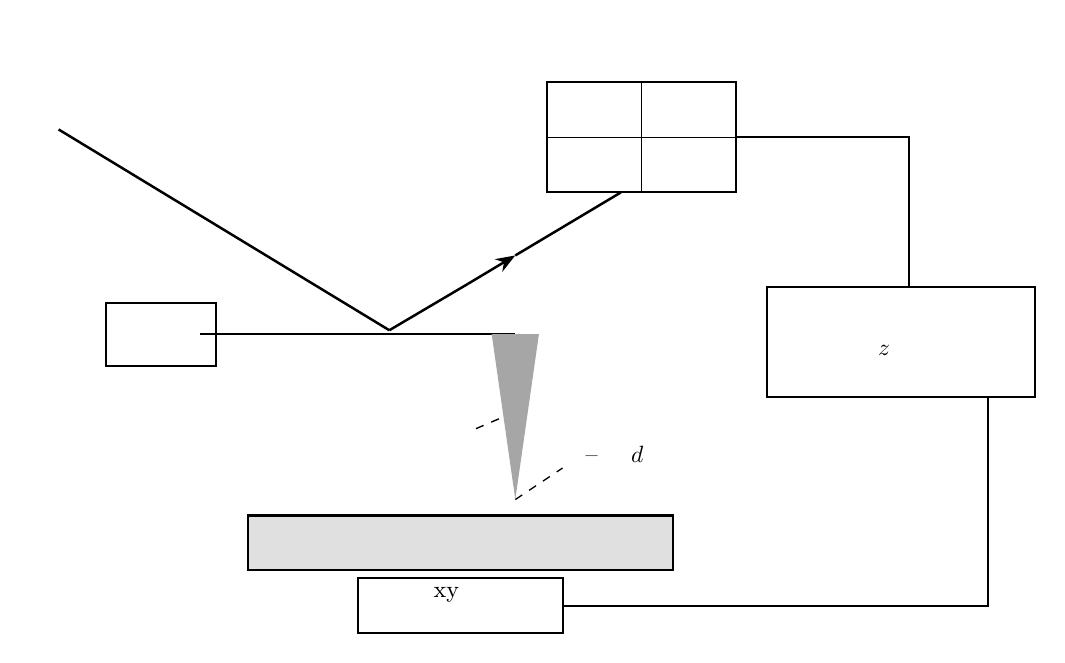
\begin{tikzpicture}[x=1mm,y=1mm,>=Stealth]
% ---- 坐标区间静态核算（x=1mm，y=1mm；版心 165 mm）----
% 图元：样品矩形 (30,10)-(84,17)；xy 扫描管 (44,2)-(70,9)；悬臂支架 (12,36)-(26,44)；
%       悬臂线 y=40（x 24→64）；针尖三角 (61,40)-(67,40)-(64,19)；
%       四象限探测器 (68,58)-(92,72)；反馈盒 (96,32)-(130,46)。
% 节点区间（anchor 已注明，宽度按 text width 计）：
%  N1 样品标签   中心(57,13.5) w48 → x[33,81]  y[11.0,16.0]  在样品矩形内
%  N2 扫描管标签 中心(57,5.5)  w24 → x[45,69]  y[ 2.5, 8.5]  在扫描管内
%  N3 支架标签   (2,34) north west w18 → x[ 2,20] y[25,34]
%  N4 针尖标签   (58,28) east     w13 → x[45,58] y[25.5,30.5]
%  N5 间距标签   (70,23) west     w30 → x[70,100] y[18.5,27.5]
%  N6 探测器标签 (80,73) south    w32 → x[64,96] y[73,81]
%  N7 激光标签   (2,68) south west w16 → x[ 2,18] y[68,77]
%  N8 反馈标签   中心(113,39) w32 → x[97,129] y[36,42]  在反馈盒内
% 两两求交核算（只列有风险的组合，均已排除）：
%  N3∩N4：x [2,20]∩[45,58]=∅；N4∩N5：x [45,58]∩[70,100]=∅；
%  N5∩反馈盒：y [18.5,27.5]∩[32,46]=∅；N5∩样品矩形：y 18.5>17；
%  N6∩探测器矩形：y 73>72；N7∩入射光束：光束在 x≤20 处 y≥57.7<68；
%  N1/N2 均在矩形内部；N8 在反馈盒内部（x 97..129 ⊂ 96..130，y 36..42 ⊂ 32..46）。
% 最大 x 坐标 = 130（反馈盒右边），最右节点文字到 x=129，故图宽 128 mm < 132 mm（\onecolwidth）。
% 控制线走 x=124（y 32→5.5），探测器信号线走 x=114（y 65→46），二者 x 不交，且都不与 N5 相交。
% ---- 样品与扫描管 ----
\fill[black!12] (30,10) rectangle (84,17);
\draw[axisline] (30,10) rectangle (84,17);
\draw[mainline] (30,17)--(84,17);
\node[align=center, text width=48mm] at (57,13.5) {样品（导体或绝缘体）};
\draw[axisline] (44,2) rectangle (70,9);
\node[align=center, text width=24mm] at (57,5.5) {xy 扫描管\\（压电陶瓷）};
% ---- 悬臂、支架与针尖 ----
\draw[axisline] (12,36) rectangle (26,44);
\node[align=left, text width=18mm, anchor=north west] at (2,34) {微悬臂\\与支架};
\draw[mainline] (24,40)--(64,40);
\fill[black!35] (61,40)--(67,40)--(64,19)--cycle;
\node[align=center, text width=13mm, anchor=east] at (58,28) {针尖};
\draw[thinline,dashed] (59,28)--(62.5,29.5);
% ---- 激光光路（入射 6,66 → 48,40.5；反射 48,40.5 → 77.4,58）----
\draw[mainline] (6,66)--(48,40.5);
\draw[mainline] (48,40.5)--(58,46.4);
\draw[mainline,->] (58,46.4)--(64,50.0);
\draw[mainline] (64,50.0)--(77.4,58);
\node[align=left, text width=16mm, anchor=south west] at (2,68) {激光\\二极管};
% ---- 四象限探测器 ----
\draw[axisline] (68,58) rectangle (92,72);
\draw[thinline] (80,58)--(80,72);
\draw[thinline] (68,65)--(92,65);
\node[align=center, text width=32mm, anchor=south] at (80,73) {四象限\\光电探测器};
% ---- 反馈控制 ----
\draw[axisline] (96,32) rectangle (130,46);
\node[align=center, text width=32mm] at (113,39) {反馈控制器与\\$z$ 压电陶瓷};
\draw[axisline] (92,65)--(114,65)--(114,46);
\draw[axisline] (124,32)--(124,5.5)--(70,5.5);
% ---- 针尖--样品间距标注 ----
\node[align=left, text width=30mm, anchor=west] at (70,23) {针尖--样品间距 $d$\\（示意，已放大）};
\draw[thinline,dashed] (64,19)--(70,23);
\end{tikzpicture}
\caption{光束偏转法 AFM 的原理示意。读者应看三条通路：悬臂偏转改变反射光方向，光斑在
四象限探测器上的位移给出偏转量；探测器信号送入反馈控制器，控制器驱动 $z$ 压电陶瓷使
针尖--样品间距回到设定值；扫描管在 $xy$ 平面内移动样品，记录的 $z$ 位移即形貌通道。
图中针尖--样品间距为便于作图已放大，实际成像时间距在纳米量级；悬臂弹性常数 $k$ 把
偏转量换算为力（$F=k\Delta z$）。本图为按工作原理重画的示意图，不代表具体仪器尺寸。
\schemamark\figsrc{据 S2 图 12-21（b），书内 p.913--914 / PDF p.399--400 重绘。}}
\label{fig:afm-setup}
\end{figure}

\subsection{成像模式与力--距离曲线}
\label{sec:afm-modes}

AFM 主要有三种基本工作模式：接触模式（contact mode）、轻敲模式（tapping mode）与非接触
模式（non-contact mode）。三者的共同点是：针尖在样品表面扫描时，样品--表面相互作用力的
改变使悬臂的偏转或振动模式改变，通过检测这一改变来反映表面的形貌或力学特征；差别在于
\textbf{把哪一个量送进反馈回路}，由此决定了工作距离、横向力大小与适用的样品范围
\src{S2 §12.3.2，书内 p.914 / PDF p.400}。

\subsubsection{接触模式：以静态偏转为反馈量}

接触模式又称静态 AFM，直接以悬臂的偏转作为力的度量。针尖与样品距离很远时悬臂处于零偏转
位置；针尖靠近或远离表面时针尖--表面作用力改变，悬臂偏转程度随之改变。偏转程度作为反馈
参数送给反馈控制器，控制器通过反馈运算控制 $z$ 方向压电陶瓷向上或向下运动，以保持恒定的
针尖--样品相互作用力；记录 $z$ 压电陶瓷的运动信号即反映样品形貌
\src{S2 §12.3.2，书内 p.914--915 / PDF p.400--401}。

静态 AFM 扫描时针尖通常与表面直接接触：这样能获得较好的分辨率，但容易损坏样品。采用较软
的悬臂（使其末端原子键能小于表面原子键能）可以减少对表面的损伤，但针尖靠近表面时又更
容易发生不受控制的跳变接触（jump-to-contact），导致难以稳定成像。正是为了回避这一对矛盾，
AFM 才发展出动态模式\src{S2 §12.3.2，书内 p.915 / PDF p.401}。这里要注意一个判断顺序：
"接触模式分辨率最高"这句话只在硬而平整的样品上成立；对软样品，横向剪切力造成的形变会同时
降低分辨率并改变高度读数。

\subsubsection{轻敲模式：以振幅（或相位）为反馈量}

轻敲模式是目前大气环境或液体中 AFM 最常用的工作模式。它把微悬臂以固定频率和振幅驱动振动，
振幅一般相对较大（\qtyrange{20}{100}{nm}），反馈信号取悬臂的振动\textbf{振幅或相位}。
轻敲模式对样品的损坏小，适用于不同的材料，具微米级扫描范围，对表面起伏程度大的样品适应性
好，且能在大气和液体中工作；代价是响应时间比较长、扫描速度较慢
\src{S2 §12.3.2，书内 p.915 / PDF p.401}。

轻敲模式之所以能同时给出"形貌"与"力学"两套信息，是因为它有两个可记录通道：振幅通道用于
反馈（维持设定振幅），相位通道是自由量。相位滞后反映针尖与样品相互作用的能量耗散与局部
黏弹性差异，因此\textbf{相位像常常比高度像更能区分同高度的不同组分}（例如载体上的金属
颗粒与载体本身）。但相位像不能按高度解读，这是本节后面单独列出的误判之一。

\subsubsection{非接触模式：以共振频率偏移为反馈量}

非接触式 AFM（non-contact AFM，NC-AFM）常用于真空环境。按检测信号与反馈参数，它又分为
振幅调制模式（amplitude-modulation mode，AM mode）与频率调制模式（frequency-modulation
mode，FM mode）。后者（FM-AFM）是动态 AFM 中较易取得原子级空间分辨率的工作模式：微悬臂
振幅一般小于 \qty{5}{nm}，反馈参数是悬臂共振频率的偏移，而共振频率的变化直接反映了
针尖--样品表面间的相互作用力梯度。近年来 Giessibl 发明的 qPlus 型传感器经不断改进，空间
分辨率达到亚原子级，已成功实现单分子内的原子分辨，是目前 AFM 技术与应用研究的前沿
\src{S2 §12.3.2，书内 p.915 / PDF p.401}。

动态 AFM 能够有效消除不稳定的针尖--样品接触，还能减小偏转测量中的噪声影响，因此目前
实际操作的多数是动态 AFM 模式（轻敲与非接触）
\src{S2 §12.3.2，书内 p.915 / PDF p.401}。三种模式的对比见表~\ref{tab:afm-modes}。

\begin{table}[htbp]
\centering
\caption{AFM 三种基本工作模式的对比}
\label{tab:afm-modes}
{\srcsize
\begin{tabularx}{\columnwidth}{@{}lXXX@{}}
\toprule
对比项 & 接触模式（静态 AFM） & 轻敲模式 & 非接触模式 \\
\midrule
反馈量 & 悬臂静态偏转（等价于 $z$ 位移） & 振动振幅（相位为附加通道） & 共振频率偏移 $\Delta f$（FM）或振幅（AM） \\
横向力 & 大：针尖与表面持续接触并剪切 & 小：间歇接触 & 几乎为零：不接触 \\
悬臂振幅 & 无（静态工作） & \qtyrange{20}{100}{nm} & 一般 $<\qty{5}{nm}$；qPlus 可达 \qty{100}{pm} \\
常用环境 & 大气、液体（须抑制毛细力） & 大气、液体（最常用） & 超高真空（FM 为主） \\
适用样品 & 硬、平整、与基底结合牢固 & 软样品、起伏大、松散颗粒 & 平整单晶，绝缘体亦可 \\
横向分辨率 & 理想条件下可达原子级 & 通常 \qtyrange{1}{10}{nm} & 原子级；FM-qPlus 达亚原子级 \\
主要优点 & 结构简单、速度快、可同步测摩擦 & 损伤小、稳定性好、环境适应性好 & 不损伤表面，可获得短程力主导衬度 \\
常见假象 & 划痕与拖拽，软样品被压陷 & 相位像被误当形貌，探针污染后衬度失真 & 长程力背景未扣除，振幅设定不当 \\
\bottomrule
\end{tabularx}}
\src{S2 §12.3.2，书内 p.914--915 / PDF p.400--401}
\end{table}

\subsubsection{动态 AFM 的谐振子模型：频率偏移为什么反映力梯度}

理解动态模式的反馈量，需要一个最小的力学模型。在动态 AFM 中微悬臂以其共振频率振动，
整个微悬臂系统可近似为一个处于外界激励力下的弹簧谐振子；针尖--样品作用力
$F_{\mathrm{ts}}$ 可看作对悬臂简谐振动的微扰，此时微悬臂是受迫阻尼振动。由此可得到微悬臂
的三个重要性质参数：弹性常数 $k$、共振频率 $\omega$ 与品质因数 $Q$
\src{S2 §12.4，书内 p.915 / PDF p.401}。

\begin{principle}
\textbf{第一步，针尖远离表面}（$F_{\mathrm{ts}}=0$）：微悬臂只受外界激励力 $F_{\mathrm{drive}}$
与阻尼作用 $F_{\mathrm{frict}}$。取余弦激励 $F_{\mathrm{drive}}=F_0\cos\omega t$（$F_0$ 为
激励振幅，$\omega$ 为激励频率），阻尼摩擦力与速度成正比 $F_{\mathrm{frict}}=m\gamma\,\dd z/\dd t$
（$m$ 为振子质量，$\gamma$ 为阻尼系数），振子离平衡位置的距离为 $z$，则受迫振动方程为
\src{S2 §12.4.1，书内 p.916 / PDF p.402}：
\end{principle}

\begin{equation}\label{eq:afm-driven}
m\frac{\dd^{2}z}{\dd t^{2}}=-kz-m\gamma\frac{\dd z}{\dd t}+F_0\cos\omega t
\end{equation}

式中 $k$ 为弹性常数。对自由谐振子，弹性常数与自然共振频率 $\omega_0$ 之间存在关系
$\omega_0=\sqrt{k/m}$；品质因数定义为 $Q=\omega_0/\gamma$：

\begin{equation}\label{eq:afm-q}
\omega_0=\sqrt{\frac{k}{m}},\qquad Q=\frac{\omega_0}{\gamma}
\end{equation}

给定参数后式~\eqref{eq:afm-driven} 有解析解，其解包含初始激励导致的瞬态项与稳定项；
经过足够长时间衰减之后，振动可近似为 $z=A\cos(\omega t-\varphi)$，振幅 $A$ 与相位偏移
$\varphi$ 都是激励频率的函数\src{S2 §12.4.1，书内 p.916 / PDF p.402}：

\begin{equation}\label{eq:afm-amp}
A(\omega)=\frac{F_0/m}{\sqrt{\left(\omega^{2}-\omega_0^{2}\right)^{2}+\left(\omega\omega_0/Q\right)^{2}}}
\end{equation}

\begin{equation}\label{eq:afm-phase}
\tan\varphi=\frac{\omega\omega_0/Q}{\omega_0^{2}-\omega^{2}}
\end{equation}

即外界激励下悬臂的运动仍是余弦函数，振动频率等于激励频率 $\omega$，但相对激励力有一个相位
延迟 $\varphi$。式~\eqref{eq:afm-amp} 与式~\eqref{eq:afm-phase} 是后面所有动态模式读数的
基础：\textbf{振幅在共振时取极大，相位在共振时过 $90$°，因此"把激励频率定在何处"直接
决定了反馈量对力变化的灵敏度}。

\textbf{第二步，针尖靠近表面}，且先假设针尖--表面相互作用力在平衡位置附近随距离线性变化。
此线性近似下，力梯度可等效为一个新的弹簧弹性常数
$k_{\mathrm{ts}}=-\left.\partial F_{\mathrm{ts}}/\partial z\right|_{z=0}$，运动方程中的
$k$ 变为 $k+k_{\mathrm{ts}}$，由此定义有效弹性力常数 $k_{\mathrm{eff}}=k+k_{\mathrm{ts}}$
与有效共振频率 $\omega_{\mathrm{eff}}=\sqrt{k_{\mathrm{eff}}/m}$。针尖--表面作用力一般远
小于悬臂回复力，即 $\left|k_{\mathrm{ts}}\right|\ll k$，于是共振频率相对自然共振频率的
偏移可近似为\src{S2 §12.4.2，书内 p.917 / PDF p.403}：

\begin{equation}\label{eq:afm-domega-lin}
\Delta\omega=\omega_{\mathrm{eff}}-\omega_0\approx\omega_0\frac{k_{\mathrm{ts}}}{2k}
=-\frac{\omega_0}{2k}\left.\frac{\partial F_{\mathrm{ts}}}{\partial z}\right|_{z=0}
\end{equation}

式~\eqref{eq:afm-domega-lin} 的结论很干净：\textbf{共振频率偏移正比于针尖--表面相互作用力
的梯度}。对正的作用力梯度（$\partial F_{\mathrm{ts}}/\partial z>0$，即吸引随靠近而增强），
$\Delta\omega<0$，共振频率向低频移动；对负的作用力梯度，共振频率向高频移动。注意源书同时
提醒：实际条件下若振动幅度较大，线性假设失效，因此该方法不能直接用于定量分析，但谐振子
模型给出的解析结果对理解动态 AFM 工作原理仍然非常有价值
\src{S2 §12.4.2，书内 p.917 / PDF p.403}。

\textbf{第三步，回到实际工作状态}。振幅调制 AFM 的振幅很大（典型约 \qty{50}{nm}），线性
近似已经失效：激励频率固定且往往接近或等于自然共振频率，针尖在一个振动周期内可深入排斥力
区与吸引力区。但实验与数值计算都证明，\textbf{悬臂振动幅度随针尖--样品间距的减小而线性
下降}，因此以振幅作为线性反馈信号来控制针尖与样品的距离依然十分有效，这也是振幅调制 AFM
被广泛使用的一个原因\src{S2 §12.4.3，书内 p.917 / PDF p.403}。

频率调制 AFM 则始终把激励频率保持在实际共振频率附近（$\omega\approx\omega_0$）。在针尖--
表面间的非线性作用下，悬臂频率偏移为\src{S2 §12.4.3，书内 p.917--918 / PDF p.403--404}：

\begin{equation}\label{eq:afm-domega-fm}
\Delta\omega=-\frac{\omega_0}{A^{2}k}\left\langle F_{\mathrm{ts}}\,z\right\rangle
\end{equation}

其中 $\left\langle F_{\mathrm{ts}}\,z\right\rangle$ 定义为一个振动周期内的平均：

\begin{equation}\label{eq:afm-fz}
\left\langle F_{\mathrm{ts}}\,z\right\rangle
\equiv\frac{1}{T}\int_{0}^{T}F_{\mathrm{ts}}\left(d+A\sin\omega t\right)A\sin\omega t\,\dd t,
\qquad T=\frac{1}{\omega_0}
\end{equation}

可以看出，频率偏移正比于 $\left\langle F_{\mathrm{ts}}\,z\right\rangle$，即一个振动周期 $T$
内针尖--样品作用力与针尖--样品距离乘积的平均。特别地，当悬臂振幅很小时（约 \qty{100}{pm}），
可用线性近似结果，$\Delta\omega$ 简化为式~\eqref{eq:afm-domega-lin}，即频率偏移正比于
针尖--表面相互作用力梯度\src{S2 §12.4.3，书内 p.918 / PDF p.404}。

\tocheck{未对照原页面图像：式~\eqref{eq:afm-domega-fm} 的分母，源文 OCR 作 $A^{2}k$；
按 Giessibl 原始推导，相同定义的 $\left\langle F_{\mathrm{ts}}z\right\rangle$ 前应为
$2kA^{2}$。此处暂按源文形式排，待核原页面后再定是否补因子 2。}

这一小振幅条件正是 qPlus 的工作点：其石英音叉弹性常数很高（$k=\qty{1800}{N/m}$），因此
可以稳定地以 \qty{100}{pm} 量级的振幅振动，刚好工作在线性近似区域；又因为短程力梯度很大，
可有效消除长程力背景对成像的影响，获得短程力主导的成像衬度，使 AFM 超越了 STM 的分辨，
达到亚原子分辨层次\src{S2 §12.4.3，书内 p.918 / PDF p.404}。

\subsubsection{力--距离曲线能给出什么}
\label{sec:afm-forcecurve}

前一小节说明的是悬臂本身；把针尖停在某一点、让 $z$ 压电陶瓷走一条"逼近--回撤"的曲线，
同时记录悬臂偏转，就得到\textbf{力--距离曲线}（force--distance curve）；在每个像素都做一次
即成\textbf{力学谱}（force spectroscopy / 空间分辨力学谱）。

\begin{measure}
测力曲线时必须同时记录并给出的条件有：悬臂弹性常数 $k$ 及其标定方法、针尖半径 $R$、
$z$ 压电陶瓷的位移量程与速度、环境（真空/干燥气/大气/液体）与温度。曲线横轴有两种取法：
一是 $z$ 压电位移，二是针尖--样品间距 $d$；两者在接触区相差悬臂偏转量 $\Delta z$，
换算关系就是胡克定律\src{S2 §12.3.2，书内 p.914 / PDF p.400}：

\begin{equation}\label{eq:afm-hooke}
F=k\,\Delta z
\end{equation}

因此未给出 $k$ 的力曲线只能做相对比较，不能给出力的绝对值。
\end{measure}

一条完整的力--距离曲线（图~\ref{fig:afm-forcecurve}）可直接读出三个量：

\begin{itemize}
\item \textbf{黏附力（最大吸引力）}：回撤支上针尖脱离表面处的跳离点，对应偏转的极大值
$\Delta z_{\max}$，由式~\eqref{eq:afm-hooke} 得 $F_{\mathrm{ad}}=k\,\Delta z_{\max}$。
它反映针尖与表面之间所有吸引作用之和。
\item \textbf{刚度（弹性模量）}：接触区曲线斜率即有效刚度 $\dd F/\dd d$；在弹性接触模型下
可由斜率反推材料的有效弹性模量，但需要已知针尖半径 $R$ 与接触几何。
\item \textbf{过零距离与短程力特征}：总力为零处对应近似成键距离；最大吸引的位置与大小、
以及短程力的梯度，是与元素种类直接相关的量（§\ref{sec:afm-app} 中单原子区分的依据）。
\end{itemize}

\begin{figure}[htbp]
\centering
\begin{tikzpicture}
\begin{axis}[
  width=\onecolwidth, height=6.2cm,
  xlabel={针尖--样品间距 $d$ / nm},
  ylabel={相互作用力（模型单位）},
  xmin=0.15, xmax=1.5, ymin=-0.22, ymax=0.5,
  xtick={0.2,0.4,0.6,0.8,1.0,1.2,1.4},
  ytick={-0.1,0,0.1,0.2,0.3,0.4,0.5},
  % 图例必须放在轴内：实测 legend pos=outer north east 会把整图撑到 483 pt（170 mm），
  % 超出 165 mm 版心 13.9 pt，成为 overfull 的唯一根因。轴内放置后整图约 133 mm。
  legend pos=north east, legend cell align=left,
]
\addplot[domain=0.185:1.5,samples=400,mainline,black]
  {0.34*exp(-(x-0.26)/0.075)-0.34/(1+((x-0.26)/0.12)^2)};
\addlegendentry{总力 $F_{\mathrm{ts}}$}
\addplot[domain=0.185:1.5,samples=400,thinline,black,dashed]
  {-0.34/(1+((x-0.26)/0.12)^2)};
\addlegendentry{长程吸引（范德华）}
\addplot[domain=0.185:1.5,samples=400,thinline,black,dotted]
  {0.34*exp(-(x-0.26)/0.075)};
\addlegendentry{短程排斥（Pauli）}
\draw[thinline,dashed] (axis cs:0.26,-0.22)--(axis cs:0.26,0.5);
% 注释节点坐标区间静态核算（数据域 x 0.15--1.5、y -0.22--0.5，轴盒约 117 mm x 50 mm）：
%  N-a 零力点  (0.30,0.30) south west w40mm → x[0.30,0.76] y[0.30,0.47]
%  N-b 图例（轴内 north east）              → x[0.98,1.50] y[0.33,0.50]
%  N-c 吸引区  (0.85,0.16) west w22mm      → x[0.85,1.10] y[0.13,0.19]
%  N-d 黏附力  (0.41,-0.17) west w46mm     → x[0.41,0.94] y[-0.20,-0.14]
% 两两求交：N-a∩N-b x 不交(0.76<0.98)；N-c∩N-b y 不交(0.19<0.33)；N-d 距曲线最近约 1.2 mm；
% N-d 下边界 -0.20 > ymin -0.22，不会被轴裁掉。
\node[align=left, text width=40mm, anchor=south west] at (axis cs:0.30,0.30)
  {零力点 $\approx$ 成键距离（$d\approx\qty{0.26}{nm}$）};
\draw[thinline,dashed] (axis cs:0.335,-0.118)--(axis cs:0.335,-0.17);
\draw[thinline,dashed] (axis cs:0.335,-0.17)--(axis cs:0.40,-0.17);
\node[align=left, text width=46mm, anchor=west] at (axis cs:0.41,-0.17)
  {最大吸引即黏附力的来源};
\node[align=left, text width=22mm, anchor=west] at (axis cs:0.85,0.16) {吸引区};
\end{axis}
\end{tikzpicture}
\caption{针尖--样品相互作用力随间距的变化（示意模型曲线）。读者应看三处：$d$ 大于零力点时
总力为吸引且随间距增大缓慢趋零（长程范德华项）；$d\approx\qty{0.26}{nm}$ 处总力过零
（近似成键距离）；$d$ 小于该值时总力转为排斥并急剧上升（Pauli 排斥，曲线在纵轴顶端被截断）。
虚线为长程吸引分量，点线为短程排斥分量，实线为两者之和。横轴为针尖--样品间距；实测力曲线
的横轴通常是 $z$ 压电位移，两者在接触区相差悬臂偏转量。本图为按长程吸引与短程排斥两项叠加
计算的示意曲线，纵轴为模型单位而非实测力值，不代表任何具体针尖--样品组合。
\modelmark\figsrc{据 S2 图 12-21（a），书内 p.913--914 / PDF p.399--400 改绘并简化。}}
\label{fig:afm-forcecurve}
\end{figure}

为什么力曲线比形貌像更接近"材料性质"？关键在两种数据的性质不同。形貌像的高度是\textbf{反馈
回路维持设定点所需的 $z$ 位移}：它把针尖--样品作用力的空间变化压成一条等值面，等值面上
任意两点只要"力相同"就显示为同一高度，几何起伏、电子态差异、吸附层与形变被混在一起，
无法分离。力曲线是逐点的 $F(d)$，直接给出作用力的\textbf{绝对值与距离依赖}：最大吸引、
过零距离、短程力梯度都由针尖原子与表面原子的种类和成键决定。因此，力学谱可以在不同针尖、
不同实验之间通过归一化比较（§\ref{sec:afm-app} 的 Sn/Si、Pb/Si 比值就是例子），而形貌像
的亮度只有相对意义。定量化弹性模量还需要额外条件（已知 $R$、标定过的 $k$、接触模型适用），
这一点不能省略。

\subsubsection{针尖卷积：图像是针尖与样品的形态卷积}
\label{sec:afm-conv}

AFM 的横向分辨率不由衍射极限决定，而由\textbf{针尖末端的形状与半径 $R$} 决定：测得的图像
是针尖形态与样品形态的"叠加"（几何上即两者的 Minkowski 和），凡比针尖更尖、更陡的结构都
会被针尖"描圆"。

\begin{principle}
设针尖末端为半径 $R$ 的球，样品上有一个半径为 $r$ 的孤立球形颗粒（$r\ll R$），扫描时
反馈维持恒定的针尖高度。颗粒中心正上方测得的高度为 $2r$（即颗粒直径，此时正确）；在偏离
中心 $x$ 处，针尖顶点高度为 $h(x)=r-R+\sqrt{(R+r)^{2}-x^{2}}$。以半高（$h=r$）度量宽度，
得表观半高宽
\end{principle}

\begin{equation}\label{eq:tipconv}
w_{\mathrm{app}}=2\sqrt{2Rr+r^{2}}\;\approx\;2\sqrt{2Rr}\qquad(r\ll R),
\qquad
\frac{w_{\mathrm{app}}}{2r}\approx\sqrt{\frac{2R}{r}}
\end{equation}

即\textbf{表观横向尺寸随 $\sqrt{R}$ 增长、随真实尺寸的平方根减小}。取 $R=\qty{10}{nm}$、
$r=\qty{1}{nm}$，表观半高宽约 \qty{9.2}{nm}，而真实宽度只有 \qty{2}{nm}——横向尺寸被高估
约 4.6 倍。

\supp{式~\eqref{eq:tipconv} 是按球形针尖与球形特征做几何卷积的标准结果，源书未给解析式；
它假设 $r\ll R$、以半高宽度量、忽略形变与吸附层。若按颗粒底部（基底高度）度量宽度，结果为
$4\sqrt{Rr}$，数值更大。}

\begin{pitfall}
\textbf{由 AFM 像直接报粒径分布是常见错误。}识别针尖卷积的四个可用判据：同一特征在不同
扫描方向或不同针尖下宽度不同；图像中出现重复出现的相同形状（多针尖/双针尖假象）；台阶边缘
被圆弧化，圆角半径与针尖半径同量级；高宽比大的结构被"抹平"。正确做法是用已知尺寸的标样
（金胶体、光栅）标定针尖，或换用更尖的针尖（碳纳米管针尖、CO 修饰针尖、qPlus 传感器）。
在针尖未标定的情况下，AFM 给出的横向尺寸只能当作\textbf{上界}。
\end{pitfall}

\subsubsection{误判与边界}
\label{sec:afm-pitfall}

\begin{pitfall}
（1）\textbf{把 AFM 高度当作真实几何高度。}形貌通道给出的是维持设定点所需的 $z$ 位移，
其中包含吸附层（水膜、羟基、残留碳）与针尖/样品形变：大气环境下氧化物表面常覆盖一层水膜
（\pedset{厚度取 \qtyrange{0.2}{0.5}{nm} 作为教学讨论量}），台阶高度会整体偏大；软样品在
接触模式下被压陷，高度又偏小。判据是改变设定点或环境后高度是否随之改变——若改变，则读出值
不是几何高度。\\
（2）\textbf{忽略针尖卷积，用图像尺寸当真实尺寸。}见式~\eqref{eq:tipconv}：常见针尖
（$R$ 为几纳米至几十纳米）会把纳米颗粒的横向尺寸放大数倍。颗粒计数得到的粒径分布、岛宽度、
孔口尺寸都受此影响。\\
（3）\textbf{把轻敲相位像当成纯形貌像。}相位滞后反映能量耗散与局部黏弹性，与高度不是同一
物理量；相位像与高度像经常不相关甚至反相。用相位像的高低谈"几何高低"是错的，但用相位像
区分同高度的不同组分（金属颗粒与载体）是恰当的用法。\\
（4）\textbf{忽略空气中吸附水膜对力曲线的影响。}针尖接近带水膜的表面时，针尖与水膜之间
形成毛细弯月面，附加一个吸引力：结果是远距离就出现吸引、跳变接触提前、黏附力偏大，
于是由曲线反推的弹性模量与最大吸引随之失真。判断方法是在干燥气氛、真空或液体中复测同一
位置，比较跳离点位置与黏附力大小。
\end{pitfall}

\subsection{原子力显微镜在催化研究中的应用}
\label{sec:afm-app}

AFM 在催化研究中的价值集中在一点：\textbf{它能在绝缘的氧化物、分子筛载体上做原子级结构
表征，并同时给出力（力学）信息}。以下五类应用按"看结构—认元素—看成键—看反应—看界面"
的顺序展开。

\subsubsection{氧化物表面结构表征}

氧化物是催化剂的常见组成部分：可作为载体负载金属纳米粒子，形成金属--氧化物界面的双活性
中心，也可作为吸光载体用于光催化。因此原子尺度的氧化物表面结构表征，对理解氧化物参与的
催化反应过程有重要意义。由于导电性较差，氧化物表面经常难以直接用 STM 观测；AFM 在绝缘体
表面也能正常工作，而且还能对针尖--表面间作用力做详细的力谱表征，为表面结构及表面吸附质
物种的判别提供更多信息。目前 AFM 已在 \ce{CeO2}(111) 和 \ce{TiO2} 等氧化物表面实现较为
清楚的原子分辨，其他重要氧化物催化剂表面如 $\alpha$-\ce{Al2O3} 也可用 AFM 实现原子级
表征\src{S2 §12.5.1，书内 p.918 / PDF p.404}。

一个特别有用的做法是\textbf{AFM 与 STM 联用}：采用导电金属针尖，在记录 AFM 信号的同时
记录隧穿电流的变化，可同时得到两套衬度。锐钛矿型 \ce{TiO2}(101) 表面就是典型例子——通过
详细对比 STM 与 AFM 图像的衬度特征，并结合第一性原理计算结果，Perez 与 Custance 等成功
识别了表面吸附水分子、次表层氧缺陷以及表面羟基。利用空间分辨的力学谱还可判定：AFM 像中的
亮度主要来自表层氧，而 STM 像中的亮点是次表层 Ti$_{5c}$ 位点。原因是 AFM 更多反映最表层
O 原子的信息，而同时记录的 STM 电流信号对表面局域电子态更敏感，因此能从电流图中看出次表层
Ti 位点；AFM 力学谱还能给出金红石型 \ce{TiO2}(110) 表面吸附金属原子与羟基的识别信息
\src{S2 §12.5.1，书内 p.918--919 / PDF p.404--405}。

\ce{CeO2}(111) 表面的氧缺陷研究进一步显示了"形貌 + 耗散"双通道的价值。\ce{CeO2}(111) 是
氧终端面，表层氧缺陷与次表层氧缺陷在 AFM 图像中表现出不同特征：表层氧缺陷表现为一个缺失
原子被周围六个突起的氧原子围绕；次表层氧缺陷则在表面没有原子缺失，但氧空位上方间距为两倍
晶格常数的三个氧原子在 AFM 图中表现突起，其内的三个相邻氧原子则向内稍微弛豫，这些实验观察
与第一性原理计算结果吻合。AFM 在记录拓扑图像时还可同时记录维持悬臂恒振幅振动的
\textbf{能量耗散信号}（dissipation signal），这种能量耗散由 AFM 针尖尖端原子与表面的相互
作用导致。Torbrugge 等通过对比 AFM 拓扑图像与能量损失信号图像发现，次表层氧空位上方三个
紧邻氧原子与针尖作用较强，其能量损失信号强于周围突起的氧原子，由此推测这些紧邻氧原子应该
比周围的氧原子具有更高的反应活性\src{S2 §12.5.1，书内 p.920 / PDF p.406}。

\tocheck{未对照原页面图像：源文在描述次表层氧缺陷形貌时标注为"图 12-22（i）"，与表层氧缺陷
同一编号，疑为（j）之误；此处只按文字描述转述，未按图号断言。}

\subsubsection{单原子尺度的元素区分}

单原子或单分子层次的化学分辨对 STM 和 AFM 一直是特别有挑战的难题，动态 AFM 的出现使这个
难题取得突破。2007 年 Custance 等利用频率调制 AFM（FM-AFM），在室温真空环境下成功实现了
Si--Sn--Pb 合金表面单个元素的化学区分
\src{S2 §12.5.2，书内 p.920 / PDF p.406}。

方法本身包含一个很值得学的归一化思想。针尖与表面之间的相互作用力有长程项（如范德华力）
与短程的化学成键作用力；他们发现虽然不同针尖会影响实验测得的针尖--表面原子力学曲线，
但\textbf{即便对于不同针尖，不同原子与针尖之间最大吸引力的比值是一个定值}。因此他们用同一
针尖测 Si、Pb、Sn 三种元素的力学曲线，并分别用该针尖在 Si 上的最大吸引力归一化，再由归一化
曲线求最大吸引力之比——这个比值与元素直接相关，例如 Sn/Si 为 $0.77$，Pb/Si 为 $0.59$。
通过这一最大力比值，就可以排除针尖因素的干扰，成功实现不同元素单个原子的区分
\src{S2 §12.5.2，书内 p.920 / PDF p.406}。

利用 AFM 力学测量技术，Gross 等还实现了识别 NaCl 表面不同荷电状态的金属原子：在同样的
针尖--样品间距下，与中性 Au$^{0}$ 原子相比，带负电的 Au$^{-}$ 与针尖的吸引力作用更大
\src{S2 §12.5.2，书内 p.920 / PDF p.406}。这两项工作合起来说明：AFM 不仅能获得氧化物负载
单原子催化剂的结构信息，还有望从原子层面理解金属--氧化物之间的电子转移规律。

\subsubsection{金属团簇内部与衬底的键合结构确认}

对负载金属纳米粒子，原子尺度的结构信息——金属内部成键及其与衬底的成键——对从根本上理解
纳米催化剂的结构--性能关系有重要作用，但长期未能取得直观的成像证据。2015 年 Giessibl 等
使用 qPlus-AFM 与 CO 分子修饰的针尖，对 Fe$_1$ 至 Fe$_{16}$ 团簇成像，成功实现了金属团簇
内部成键的观测。CO 修饰针尖极为清楚地反映了 Fe 团簇因表面吸附导致的电荷密度再分布，把表面
吸附原子的成像分辨率推到亚原子级别。作者再结合衬底的分辨图像确定成键位点：Fe 原子双聚体与
三聚体在表面的落位并不是广为人知的表面 fcc 位点，而更接近桥位（bridge）；而对于 Fe 单体与
Fe 四聚体以上的团簇，所有 Fe 都落在更稳定的表面 fcc 位\src{S2 §12.5.3，书内 p.921 /
PDF p.407}。

这个例子的方法论意义大于结论本身：\textbf{团簇尺寸改变落位}——小团簇落在低配位桥位，
大团簇回到密排的 fcc 位。这类信息直接影响对活性位结构的判断（例如金属--载体界面的配位
环境），而它只能由原子级成像给出。

\subsubsection{化学键的实空间成像与反应中间体}

qPlus-AFM 极高的空间分辨率使人可以直接观察共价键，甚至区分不同键级（bond order）的碳碳键；
而识别分子间相互作用力对揭示分子反应中间体、氢键的物理本质有重要意义。2013 年，国家纳米
中心的裘晓辉等在国际上首次实现氢键的直接观测：在 Cu(111) 表面沉积 8-羟基喹啉
（8-hydroxyquinoline，8-hq）分子，再用 qPlus-AFM 观测，发现分子聚集体之间形成了可观测的键，
结合 DFT 计算模拟以及成键位置和取向，确认为分子间氢键。由于 qPlus-AFM 对分子内成键的衬度
来源于针尖与样品原子间的 Pauli 排斥力，因此该衬度与电子密度的空间分布直接相关；分子间氢键
的成功观测，为氢键的共价键成分与 H 到 N/O 之间的电荷转移提供了直接的实验证据。作者进一步
观察到表面 Cu 吸附原子与脱氢 8-hq 之间形成金属--N 配位键，这为直接观测表面反应、表面吸附
与成键提供了可能\src{S2 §12.5.4，书内 p.922--923 / PDF p.408--409}。

反应中间体的直接观测是理解反应动力学的重要方法，但中间体活性高、表面浓度低，许多常规手段
难以获得其信息。qPlus-AFM 因为可以直接看到化学键，用于表面有机分子反应的观察时可以直接
分辨反应分子与多种反应产物。Crommie 等用 qPlus-AFM 实现了表面分子反应中间体的直接捕获与
观察：研究对象是 1,2-二（2-乙炔基苯基）乙炔在 Ag(100) 表面的交叉偶联与分子内环化反应，
作者不仅看到了反应分子和产物，还捕捉到了中间体。为了获得更多机理认识，作者把表面加热到
不同温度和时间，再用 qPlus-AFM 确定表面分子浓度，得出整个反应进程中产物与各中间体的变化。
他们发现，用经典密度泛函理论结合微观动力学无法模拟出实验观察到的中间体浓度变化，必须考虑
反应分子与表面之间的传能以及表面对不同中间体活化熵的影响，理论模拟结果才能与实验吻合。
结合理论计算与实验观察，作者得出结论：中间体在表面可以自由旋转和平动、活化熵较高，因此
参与下一步反应的速率较慢，从而可被实验观察到；而其他理论预测的中间体因为活化熵较低，
很快在反应中被消耗掉\src{S2 §12.5.4，书内 p.923--924 / PDF p.409--410}。

这一案例给催化研究者的提示是：\textbf{表面反应的选择性不只由活化焓决定，活化熵（即中间体
在表面的自由度）可以直接改变可观测的产物分布}，而 AFM 提供的是唯一能"点名"每个中间体的
实验通道。

\subsubsection{固--液界面的空间三维成像}

固--液界面的原子级观测是理解电化学与生命现象的关键。长期以来固体表面水分子的原子排列模型
都不特别明确；特别是水溶液--固体界面，由于双电层的存在，界面结构在空间上是局域变化的，
常规二维扫描很难得到界面结构在空间上的分布信息。由于 AFM 可以工作在较大的针尖--表面距离
范围，因此在三维空间上的直接观测可以解析固--液结构的完整图像
\src{S2 §12.5.5，书内 p.925 / PDF p.411}。

Fukuma 等用 AFM 直接观测了白云母片上的水分子排列，得到近表面层水分子排列图像，并结合力学
曲线获得了离固体表面垂直距离 \qty{0.78}{nm} 以内的水--固体界面三维图像。观测结果是分层
的：离白云母表面较远处，AFM 基本看不到明显衬度；针尖更加靠近表面后，$xy$ 平面截图才给出
结构。在 \qty{0.2}{mol/L} KCl 溶液中，三维 AFM 图像显示表面吸附的 K$^{+}$ 单层及其顶端
两层水合层，水合层约 \qty{0.3}{nm} 厚，随表面起伏排列；在 \qty{4}{mol/L} KCl 溶液中，
界面层分为表面约 \qty{2}{nm} 厚的有序液相层与体相溶液层；在约 \qty{5}{mol/L} NaCl 溶液中，
则得到原子级有序的白云母--溶液界面三维 AFM 图像
\src{S2 §12.5.5，书内 p.925 / PDF p.411}。

对催化而言，这类结果的意义在于把"界面水"从连续介质变成了可分层的结构：水合层厚度、
吸附离子单层与有序液相层的存在，直接决定电催化界面上的传质与双电层模型假设是否成立。

\subsubsection{读图实例：从形貌通道与耗散通道判断氧空位类型}

下面用 \ce{CeO2}(111) 氧缺陷的判别过程演示 AFM 数据的读法。观察与推断分开陈述。
形貌特征取自源文对图 12-22（i）至（o）的文字描述
\src{S2 §12.5.1，书内 p.919--920 / PDF p.405--406}。

\begin{obs}
在一张 \ce{CeO2}(111) 的原子分辨 AFM 图上（同时记录形貌通道与能量耗散通道）：
① 缺陷 A：一个亮点的位置空缺，其周围六个亮点仍按六方排列，并相对周围略微凸起，形成
"缺一个原子的六角环"；
② 缺陷 B：表面上没有亮点缺失，但空位正上方、间距为两倍晶格常数的三个亮点连成一组凸起，
该组内部的三个相邻亮点相对周围略微内凹（弛豫）；
③ 在能量耗散通道中，缺陷 B 处那三个紧邻亮点的耗散信号强于周围的凸起亮点；
④ 两类缺陷在形貌通道中的高度起伏都在亚埃量级（\pedset{本实例不给出具体高度数值，
以免被当作从原图量取的结果}）。
\end{obs}

\begin{infer}
由 ① 推断缺陷 A 是\textbf{表层氧空位}：表面直接缺失一个氧，周围氧向空位弛豫而显得凸起。
由 ② 推断缺陷 B 不能用表层空位解释（表面没有亮点缺失），只能来自表面以下的缺陷：
\textbf{次表层氧空位}通过其上方氧原子的弛豫改变了针尖--表面作用力，从而在形貌通道产生
衬度。由 ③ 进一步推断：那三个氧原子与针尖的相互作用更强，源文据此推测它们比周围的氧原子
具有更高的反应活性。把两个通道合起来还能得到一个一般结论：在 \ce{CeO2}(111) 上"AFM 亮"
对应最表层氧，而在 \ce{TiO2} 上"STM 亮"对应次表层 Ti$_{5c}$ 位点——不同通道的"亮点"
不是同一种东西，跨方法比较亮度前必须先确认衬度来源。
\end{infer}

推断的边界必须写明：如果只有形貌通道而没有耗散通道与第一性原理计算的对照，②③ 只能算
假设；形貌衬度还会随针尖状态（CO 修饰、钝化程度）整体改变甚至反相，因此判断缺陷类型时
必须报告针尖状态与设定点。

\begin{dataflow}
从原始数据到结论的链条（以上例为例）：① 探测器电压 $\rightarrow$ 悬臂偏转或振幅信号
$\rightarrow$ 扣除远离表面处的参考值后得到频移/振幅通道；② 反馈回路把该通道维持在设定点，
$z$ 压电位移即形貌通道，维持恒定振幅所需的激励功率即能量耗散通道；③ 由形貌通道的周期性
（晶格常数、缺陷间距）定标空间坐标；④ 由缺陷处的局部形貌特征 + 耗散衬度 + DFT 计算对比
判定缺陷类型；⑤ 在缺陷处取一条 $F(d)$ 力学谱，由最大吸引与短程力特征判断亮点对应哪种
原子。每一步都依赖上一步的定标：若第 ③ 步的横向定标被针尖卷积放大（式~\eqref{eq:tipconv}），
第 ④ 步"两倍晶格常数"这一判据就会失效。
\end{dataflow}

\subsubsection{互补与回查}
\label{sec:afm-crosscheck}

\begin{crosscheck}
AFM 的强项（绝缘体可用、给力与力学性质）与弱项（不给电子结构、横向尺寸受针尖卷积影响、
高度不等于几何高度）决定了它的回查路线：\\
\textbf{与 STM 联用}：同一针尖同时记录隧穿电流与力信号，可把"形貌亮"与"电子态亮"分开——
这是 \ce{TiO2}(101) 上区分表层氧与次表层 Ti 位点的关键，也适用于任何导电性刚好够用的
样品。\\
\textbf{与衍射/散射方法回查}：由 AFM 量出的晶格常数、台阶高度、缺陷间距应与 XRD/LEED
给出的体相或表面晶格一致；若偏差系统性偏大，先怀疑横向定标（针尖卷积）而不是样品。\\
\textbf{与第一性原理计算回查}：缺陷类型的判定几乎都依赖"实验形貌 + 计算模拟"的对照
（\ce{CeO2} 与 \ce{TiO2} 两个例子都是如此）；反过来，计算给出的力曲线又能预测不同元素
的最大吸引力之比，与力学谱实测比值比较。\\
\textbf{与方法边界回查}：AFM 看不到的元素种类、氧化态与体相结构，仍要靠 XPS、EXAFS、
化学吸附滴定补足；把 AFM 的形貌结论直接当"活性位归属"是越界。
\end{crosscheck}

\srcnote{本节（12.3—12.5）内容据 S2（下册）第 12 章，书内 p.913—925 / PDF p.399—411。
其中式~\eqref{eq:lj}、式~\eqref{eq:tipconv} 及毛细力讨论为按学科标准形式的补充，
已在正文中单独标注；标注 \tocheck{} 之处待对照原页面图像核验。}
}{}
\IfFileExists{chapters/parts/ch12-c.tex}{% ================================================================
%  chapters/parts/ch12-c.tex
%  第 12 章  扫描探针显微镜与纳米光谱技术（分片 c）
%  源：S2（下册）第 12 章，书内 p.926—942 / PDF p.412—428
%  范围：12.6（扫描探针与光谱技术的结合：12.6.1 近场扫描光学显微镜、
%        12.6.2 TERS、12.6.3 Nano-FTIR、12.6.4 光学激发的针尖探测方法）
%        与 12.7（结束语）
%  不含：12.1—12.2（STM，分片 a）、12.3—12.5（AFM，分片 b）
%  说明：本分片不写 \chapterstart（分片 a 已写）。
% ================================================================

\subsection{扫描探针与光谱技术的结合}
\label{sec:nano-intro}

\begin{probout}
扫描探针显微镜把空间分辨率推到了原子尺度，但常规 STM 与 AFM 给不出化学信息：表面元素组成、
吸附物种的种类与吸附构型都不在它们的输出里。本节要回答的是——\textbf{怎样在保留纳米乃至
亚纳米空间分辨率的同时，拿到分子的振动（化学）指纹}，以及为此付出的代价是什么。原始输出
有三类：逐点采集的\textbf{近场拉曼谱或近场红外谱}（峰位以 cm$^{-1}$ 计）、由某个特征峰的
强度或峰面积逐点拼出的\textbf{化学像}、以及与之同时记录的\textbf{形貌像}；此外还有一组必须
随图报告的条件（针尖材质与曲率半径、波长与功率、针尖—样品间距、解调阶数、每像素采谱时间、
环境）。本节的核心结论只有一句：\textbf{空间分辨率不再由波长（衍射极限）决定，而由针尖顶端
的曲率半径与近场增强体积决定；代价是信号极弱、探针易污染钝化、扫描极慢，并且远场背底必须被
有效抑制}。后面多种技术的差别，本质上只是这四项代价的不同付法。
\end{probout}

\paragraph{化学信息的缺口}
STM 与 AFM 之外，高空间分辨的技术在化学识别上各有短板。STM 路线上的非弹性电子隧道谱
（inelastic electron tunneling spectroscopy，IETS）已能提供原子分辨率的表面振动谱，达到了
目前分子振动谱学的空间分辨率极限；但隧穿电子的振动吸收截面极低，受信号灵敏度与隧穿结构
稳定性的限制，IETS 目前只能在极低温（通常为液氦温度）与超高真空下工作，且能探测的振动模式
相当有限\src{S2 §12.6，书内 p.926 / PDF p.412}。透射电子显微镜虽然能在原子尺度给出固体
的原子与电子结构，却常常只能对重元素成像，因此在催化表征中往往只能对纳米粒子本身、而不是
吸附分子做高分辨成像。而"表面分子与反应中间体到底是什么"恰恰是红外、拉曼等分子振动光谱
所擅长的——问题在于，这些经典光谱技术受光学衍射极限限制，其宏观平均信息在解释局域活性位
特征时经常失灵\src{S2 §12.6，书内 p.926—927 / PDF p.412—413}。

\paragraph{衍射极限：全部问题的出发点}
\begin{principle}
传统远场光学成像的空间分辨率受光波衍射限制。点光源经透镜成像时呈现艾里斑，19 世纪末
Abbe 与 Rayleigh 由此推出瑞利判据：两个点源可被清楚分辨的最小距离为
\begin{equation}\label{eq:rayleigh}
\Delta x \;\geq\; \frac{0.61\,\lambda}{n\sin\theta}
\end{equation}
式中 $\lambda$ 为照明光波长，$n\sin\theta$ 为数值孔径（numerical aperture，N.A.）。由于通常
$n<2$、$\sin\theta<1$，可分辨的最小距离一般不小于 $\lambda/2$，即成像波长的一半
\src{S2 §12.6，书内 p.927 / PDF p.413}。
\emph{核对说明}：已对照原页面图像（书内 p.927 / PDF p.413）。原书印「两个点源之间可被清楚
分辨的最小距离 $\Delta x \geq 0.61\lambda/n\sin\theta$，其中，$\lambda$ 为照明光波长，
$n\sin\theta$ 为数值孔径（numerical aperture，N.A.）」；「由于通常 $n<2$、$\sin\theta<1$，
所以可分辨的最小距离 $\Delta x$ 一般不小于 $\lambda/2$，即成像光波长的一半」；「其在可见光下
的最大空间分辨率是 $200\sim400$ nm，如果使用中红外光谱，则空间分辨率要减至几微米的量级」——
数值与变量定义均与本分片一致。原书正文是行内线性写法（OCR 亦作线性串），本分片按通行写法排
成分式，系数 $0.61$ 照录。
\end{principle}

该判据给出现成的数量级：传统光学系统在可见光下的最大空间分辨率是 200—400 nm；若使用中红外
光谱，空间分辨率要降到几微米量级\src{S2 §12.6，书内 p.927 / PDF p.413}。这正是"红外光谱
擅长化学识别、却不擅长纳米成像"的根源——红外波长本身（常用 2.5—25 µm，对应 400—
4000 cm$^{-1}$）已经从根本上限制了它的空间分辨能力。

绕开衍射极限有几条路，各自代价不同。其一是换更短的波长，例如高能电子与离子，波长可小于
一个原子，从而实现原子分辨率成像；但很高的能量通常带来严重样品损伤。其二是荧光标记：用染料
分子做化学标记，在可见光区激发、由激发态弛豫发出荧光，配合合适的滤光片与探测器可实现单分子
荧光成像；共聚焦荧光显微镜结合先进光源与探测器后，已发展出受激发射损耗显微术（STED）、
光活化定位显微术（PALM）、随机光学重构显微术（STORM）等方法，可获得远低于衍射极限的空间
分辨率。这些超分辨远场技术在生物研究中应用广泛，但\textbf{它们能提供的光谱信息仍相当有限}
\src{S2 §12.6，书内 p.927 / PDF p.413}。其三是本节的主题：把探针放进光路，用近场代替远场。
事实上在 STM 与 AFM 发明后不久，就有人尝试把扫描探针的高空间分辨与光谱的化学分辨结合起来；
目前近场光学显微镜、针尖增强光谱技术以及光学激发的针尖探测方法，都被认为具有用于催化原位
研究的潜力\src{S2 §12.6，书内 p.927 / PDF p.413}。

\subsubsection{近场扫描光学显微镜}
\label{ssec:nsom}

\paragraph{从 Synge 的小孔到第一台近场显微镜}
1928 年 Synge 提出用小孔径实现超衍射极限光学分辨率的设想：光通过小孔后高度发散，在远场中
当传播距离远大于波长与孔径时，衍射导致强度起伏、形成艾里斑；但在近场区域，只要物体足够
接近小孔，成像分辨率就能接近孔径尺寸、远小于波长\src{S2 §12.6.1，书内 p.927—928 /
PDF p.413—414}。由于当时难以对纳米尺度的间距做精确控制，这一可能性直到 1972 年才被实验
证实。STM 实现了探针对表面的快速精确扫描与针尖—样品间隙的精确控制，直接推动了近场扫描
光学显微镜（near-field scanning optical microscopy，NSOM，也称 SNOM）的开发：1984 年，
在瑞士 IBM 研究实验室工作的 Pohl 等制造了第一台用可见光测量的近场光学显微镜，通过探针在
样品表面保持数十纳米的距离采集反馈信息，并在几年后实现高分辨成像
\src{S2 §12.6.1，书内 p.928 / PDF p.414}。

\paragraph{孔径式近场显微镜：原理与它自己的天花板}
最初的方法是用金属（如 Al 或 Ag）涂覆的锥形光纤作探头（光纤底部孔径约 100 nm），借助扫描
探针的反馈机制把光纤靠近样品表面，光通过底部小孔照射样品，从而避开衍射形成的艾里斑，在
测量形貌的同时以远低于波长的分辨率成像——这就是\textbf{孔径式扫描近场显微镜}。采集方式随
样品而变：样品对探测光透明时，可在样品下方检测透射光子，或在周围检测激发的荧光；不透明
样品则检测反射光；也可以从外部照射样品、再用光纤收集光子送到探测器。其中特别值得注意的是
\textbf{光子扫描隧道显微镜}（PSTM，亦称扫描隧道光学显微镜 STOM）：光从样品背面全内反射产生
隐失波（evanescent wave），光纤探针端部检测样品表面的隐失场并把它转换为传播模式送到远处
的探测器；隐失波受样品调制，因此近场光学像携带局域样品信息，但图像解析通常较复杂，源书
称目前尚未见用于催化研究的报道\src{S2 §12.6.1，书内 p.928 / PDF p.414}。

孔径式的主要弱点在于小孔径光纤的低透过率。为补偿这一点，光源通常都是高亮度、低发散的激光；
即便如此，对 80—100 nm 的孔径，光纤传导的可见光透过率也只有 $10^{-7}$—$10^{-4}$ 量级，
即几十纳瓦的功率，空间分辨率因此严重受限。更麻烦的是透过率随孔径减小或波长变长而进一步
下降：中红外波段下 50 nm 孔径只剩 $10^{-30}$ 量级，红外近场显微镜用孔径式方案几乎不可行
\src{S2 §12.6.1，书内 p.928 / PDF p.414}。

\paragraph{散射式近场显微镜：把针尖当作纳米散射体}
为克服孔径式的限制，人们发展了散射式近场光学显微镜（scattering-type SNOM，s-SNOM）：用
激光聚焦照射扫描探针的金属针尖，在针尖附近激发一个纳米尺度的增强近场区域；针尖接近样品
表面时，由于不同物质介电性质不同，近场光学信息被改变；通过精确调整实现\textbf{焦斑—针尖—
样品三者对准}，散射光经显微物镜由远场探测器收集，再经精密的调制过滤技术解析，就能得到表面
的近场光学谱并成像\src{S2 §12.6.1，书内 p.928—929 / PDF p.414—415}。以金属针尖顶点作为
纳米散射体，s-SNOM 突破了孔径式的限制：\textbf{其空间分辨率与光学分辨率通常被认为仅由探针
针尖的曲率半径决定}，使几乎所有的光谱技术都能扩展到近场使用，成像分辨率不再受波长限制，因而
尤其适合红外与太赫兹波的微观成像，并可能具有 10 nm 或更好的空间分辨率
\src{S2 §12.6.1，书内 p.929 / PDF p.415}。

\paragraph{分辨率的来源与四项代价（本节核心）}
\begin{principle}
\textbf{分辨率来源。}近场方案把"分辨"这件事从波长转移到了探针几何上。近场（隐失）信号随
离开表面的距离迅速衰减，可用单一衰减长度 $\delta$ 描述：
\begin{equation}\label{eq:nearfield-decay}
E_{\mathrm{nf}}(z)=E_{\mathrm{nf}}(0)\,e^{-z/\delta},\qquad \delta \sim a
\end{equation}
式中 $z$ 为针尖—样品间距，$a$ 为针尖顶端曲率半径。只要间距 $z$ 与针尖曲率半径同量级，
参与相互作用的样品体积就被限制在针尖正下方，其横向尺寸由 $a$（而非 $\lambda$）决定，这就是
"分辨率由针尖曲率半径决定"的物理含义。
\emph{核对说明}：已对照原页面图像（书内 p.928—929 / PDF p.414—415）。原书对近场衰减只作
文字说明：光通过小孔在远场高度发散，而在近场区域物体足够接近小孔即可获得接近孔径尺寸、远小于
光波长的分辨率（书内 p.928）；「其空间分辨率和光学分辨率通常认为仅由扫描探针针尖的曲率半径
决定」（书内 p.929）——原书\textbf{未给出}解析式，也\textbf{未定义} $\delta$。式
~\eqref{eq:nearfield-decay} 按隐失场的标准形式补写，$\delta\sim a$ 为量级估计（隐失场衰减长度
与针尖曲率半径同量级），非原书原文。另需注意：「分辨率由针尖曲率半径决定」一语在原书中出现
于 §12.6.1 末段对散射式近场显微镜（s-SNOM）的论述；孔径式近场显微镜的分辨率则由孔径尺寸决定
（书内 p.928）。

\textbf{代价一：信号极弱。}只有针尖正下方极小的体积贡献近场信号，且信号随间距指数衰减
（式~\eqref{eq:nearfield-decay}）。这在数值上是残酷的：孔径式方案中中红外 50 nm 孔径的透过率
仅 $10^{-30}$ 量级；散射式方案中，从悬臂与针尖杆散射出来的\textbf{远场背底远强于针尖末端
散射的近场信号}。因此近场光谱的可行性从来不取决于"有没有信号"，而取决于\textbf{能不能把
极弱的近场信号从强得多的远场背底里分离出来}。

\textbf{代价二：探针易污染、易钝化。}增强场与分辨率都由针尖最末端几纳米的几何与光学性质
决定，任何吸附物、氧化层或磨损都会同时改变二者；针尖还可能与样品发生化学作用而把自身变成
催化剂（见 \ref{ssec:ters} 段的 Ag 针尖与氧化铝保护层）。

\textbf{代价三：扫描极慢。}近场信号的绝对强度低，每个点位都必须积分足够长的时间才能得到可用
谱图。源书给出的两个标尺是：同步辐射红外光源下单点谱约几秒、化学成像需几分钟；而 Gross 等
的实验中单点红外谱约需 20 min，以致只能做线扫描而无法成像。

\textbf{代价四：远场背底必须被有效抑制。}这是近场光谱与常规光谱最大的操作差别。抑制手段是
调制—解调：让针尖以频率 $\Omega$ 在 $z$ 方向振动，近场信号因式~\eqref{eq:nearfield-decay}
而被周期性调制，在探测器中产生 $n\Omega$（$n=1,2,3,4,\dots$）的谐波，未受调制的远场背底
（直流部分）则留在低频；锁相放大只提取 $n\Omega$ 分量，就压掉了背底。其数学形式就是傅里叶
分量：
\begin{equation}\label{eq:demod}
S_n=\frac{\Omega}{\pi}\int_{0}^{2\pi/\Omega} I\big(z(t)\big)\cos(n\Omega t)\,\dd t,
\qquad z(t)=\bar z+A\cos\Omega t
\end{equation}
\textbf{这四项代价是同一件事的四个侧面}：因为信号只来自极小体积，所以它弱、所以必须慢、
所以探针状态决定一切、所以必须靠调制把背底和信号分开。判断一台近场实验是否可信，就是逐条
问这四项是否被处理过。
\end{principle}

\begin{figure}[htbp]
\centering
\begin{tikzpicture}[x=1mm,y=1mm,>=Stealth]
% ---- 坐标区间静态核算（x=1mm，y=1mm；版心 165 mm，图宽上限 \onecolwidth = 132 mm）----
% 图元：样品矩形 (6,10)-(98,18)；吸附分子标记 x=40,46,52,58,64，y 18→20.5；
%       针尖多边形 (52,22.5)-(45,36)-(49,36)-(49,52)-(55,52)-(55,36)-(59,36)-cycle；
%       近场热点椭圆 中心(52,20)、rx=9、ry=4 → x[43,61] y[16,24]；
%       z 向振动双箭头 x=42，y 20→30；
%       激发光束两线 (10,70)→(52,20)、(22,70)→(52,20)；
%       近场收集线 (61,20)→(86,58)；远场背底线 (54,50)→(86,66)；
%       探测器盒 (86,56)-(126,68)。
% 节点区间（anchor 已注明；宽度按 text width 计，纵向按注1行±3.5mm、注2行±5.5mm、注3行±6.5mm）：
%  N1 样品  中心(52,14)      w44     → x[30,74]      y[12,16]      在样品矩形内
%  N2 近场区 (63.5,20) west  w26     → x[63.5,89.5]  y[18,22]
%  N3 针尖  (34,25) east     w26     → x[8,34]       y[18.5,31.5]（3 行）
%  N4 z     (40.5,26) east   自然宽   → x[35.5,40.5]  y[24,28]
%  N5 远场背底 (60,48) west  w16     → x[60,76]      y[46,50]
%  N6 近场信号 (73,34) west  w14     → x[73,87]      y[32,36]
%  N7 探测器 中心(106,62)    w34     → x[89,123]     y[58,66]      在探测器盒内
%  N8 激光  (4,72) north west w40    → x[4,44]       y[72,76]
% 两两求交核算（只列有风险的组合，均已排除）：
%  N3∩N4：x [8,34]∩[35.5,40.5]=∅（间隙 1.5 mm）；
%  N3∩激发光束：光束在 y∈[18.5,31.5] 处 x∈[43.2,52.4]，与 [8,34] 不交；
%  N4∩激发光束：光束在 y∈[24,28] 处 x∈[45.3,49.6]，与 [35.5,40.5] 不交；
%  激发光束∩z 双箭头：光束 A 在 x=42 处 y=31.9>30（箭头顶端），不相交；
%  N2∩近场收集线：收集线在 y∈[18,22] 处 x∈[59.7,62.3]，与 [63.5,89.5] 不交；
%  N6∩近场收集线：收集线在 y∈[32,36] 处 x∈[68.9,71.5]，与 [73,87] 不交；
%  N5∩近场收集线：收集线在 y∈[46,50] 处 x∈[78.1,80.7]，与 [60,76] 不交；
%  N5∩远场背底线：背底线在 x∈[60,76] 处 y∈[53,61]，与 [46,50] 不交；
%  N6∩远场背底线：y 32..36 与 59.5..66 不交；N6∩N5：y [32,36]∩[46,50]=∅；
%  N5／N6∩探测器盒：x ≤87 < 86? 否——N6 x 至 87>86，但 y 36<56，故不相交；
%  N8∩激发光束：光束起点 y=70<72；N8∩探测器盒：y 72>68；
%  样品矩形∩N3：N3 y 下界 18.5>18；分子标记 x 40..64 与 N3 x ≤34 不交。
% 最大 x 坐标 = 126（探测器盒右边），最右文字到 x=123；最小 x = 4（N8 左界）。
% 故图宽 ≈ 122 mm < 132 mm（\onecolwidth），图高 ≈ 66 mm。
% ---- 样品与表面吸附分子层 ----
\fill[black!10] (6,10) rectangle (98,18);
\draw[axisline] (6,10) rectangle (98,18);
\node[align=center, text width=44mm] at (52,14) {样品与表面吸附分子层};
\foreach \p in {40,46,52,58,64}{\draw[thinline] (\p,18) -- (\p,20.5);}
% ---- 金属针尖（同时是光学天线）----
\fill[black!25] (52,22.5) -- (45,36) -- (49,36) -- (49,52) -- (55,52) -- (55,36) -- (59,36) -- cycle;
\draw[mainline] (52,22.5) -- (45,36) -- (49,36) -- (49,52) -- (55,52) -- (55,36) -- (59,36) -- cycle;
\node[anchor=east, align=right, text width=26mm] at (34,25) {金属针尖（Ag/Au、PtSi）};
% ---- 近场增强区：横向尺寸由针尖曲率半径决定 ----
\fill[black!8] (52,20) ellipse [x radius=9, y radius=4];
\draw[dashed, accentsoft] (52,20) ellipse [x radius=9, y radius=4];
\node[anchor=west, align=left, text width=26mm] at (63.5,20) {近场增强区};
% ---- 针尖 z 向振动（频率 Ω，锁相解调其 nΩ 分量）----
\draw[<->, accent] (42,20) -- (42,30);
\node[anchor=east] at (40.5,26) {$z$};
% ---- 聚焦激光：焦斑远大于针尖 ----
\draw[thinline] (10,70) -- (52,20);
\draw[thinline] (22,70) -- (52,20);
\node[anchor=north west, align=left, text width=40mm] at (4,72) {聚焦激光（焦斑远大于针尖）};
% ---- 近场信号与远场背底走同一路光 ----
\draw[->, mainline] (61,20) -- (86,58);
\draw[->, mainline] (54,50) -- (86,66);
\node[anchor=west, align=left, text width=14mm] at (73,34) {近场信号};
\node[anchor=west, align=left, text width=16mm] at (60,48) {远场背底};
% ---- 探测器与锁相解调 ----
\fill[black!6] (86,56) rectangle (126,68);
\draw[axisline] (86,56) rectangle (126,68);
\node[align=center, text width=34mm] at (106,62) {探测器 + 锁相解调（$n\Omega$）};
\end{tikzpicture}
\caption{针尖—样品近场耦合与远场背底抑制的几何。读者应看三件事：① 参与相互作用的样品体积
由针尖顶端的\textbf{近场增强区}决定，其横向尺寸与针尖曲率半径同量级，与聚焦焦斑（微米量级）
无关——这是"分辨率不再受衍射极限限制"的几何来源；② 近场信号与来自针尖杆、悬臂的\textbf{远场
背底}走的是同一路散射光，进入同一个探测器，因此必须靠针尖 $z$ 向振动（频率 $\Omega$）调制、
再锁相解调 $n\Omega$ 分量才能把二者分开（式~\eqref{eq:demod}）；③ 近场信号随间距 $z$ 指数
衰减（式~\eqref{eq:nearfield-decay}），所以针尖必须始终停在距表面几纳米处，这也正是探针
污染、磨损与会话式扫描缓慢的根本原因。图为示意，不按真实比例（真实针尖—样品间距约几纳米，
而焦斑为微米量级）。\schemamark\figsrc{据 S2（下册）§12.6.1，书内 p.927—929 / PDF p.413—
415 正文改绘。}}
\label{fig:snom-geometry}
\end{figure}

\begin{figure}[htbp]
\centering
\begin{tikzpicture}
\begin{axis}[
  width=\onecolwidth,
  height=6.2cm,
  xlabel={针尖—样品间距 $z$ / nm},
  ylabel={归一化信号强度},
  xmin=0, xmax=20, ymin=1e-5, ymax=3,
  ymode=log, log basis y=10,
  ytick={1e-4,1e-3,1e-2,1e-1,1},
  yticklabels={$10^{-4}$,$10^{-3}$,$10^{-2}$,$10^{-1}$,$1$},
  xtick={0,5,10,15,20},
  domain=0:20, samples=200,
  legend pos=north east,
  legend cell align=left,
]
\addplot[accent, solid] {exp(-x/2)};
\addlegendentry{近场信号 $\propto e^{-z/\delta}$（$\delta=2$ nm）}
\addplot[black, dashed] {0.01};
\addlegendentry{远场背底（取为接触时近场的 $1\%$）}
\addplot[black!55, dotted, line width=1.4pt] {1e-4};
\addlegendentry{高次解调（$n\Omega$）后的残余背底}
\end{axis}
\end{tikzpicture}
\caption{为什么近场实验"必须靠近、必须解调"——一个只用于说明数量级关系的模型曲线。实线是
式~\eqref{eq:nearfield-decay} 取 $\delta=2$ nm 的近场信号；虚线是远场背底，示意性地取为接触
时近场信号的 $1\%$；点线是经高次解调后残余的背底。读者应看交点：\textbf{若不做任何抑制},
针尖退到约 9 nm 以外，近场信号就落到背底之下；把背底再压低两个数量级，可用的工作距离才
扩展到约 18 nm。结论不是这两个具体数字，而是"可用工作距离由近场信号与残余背底之比决定"。
\modelmark 曲线为模型计算，非实测数据；衰减长度与背底比例均为示意值，源书未给出。
\emph{核对说明}：已对照原页面图像（书内 p.929、p.936 / PDF p.415、p.422）。原书只作定性
说明：「由于从 AFM 探针悬臂和针尖散射出来的远场背景信号远强于从 AFM 针尖末端散射出来的近场
信号，因此必须对近场红外信号的光强进行调制」；「通过锁相放大处理就可提取这些近场信号，同时
剔除未受调制的背景信号（直流部分）」（书内 p.936）。原书\textbf{未给出}曲线与数值：本图的衰减
长度 $\delta=2$ nm、背底取接触时近场信号的 $1\%$、高次解调后再降两个数量级，均为示意取值，
只用于说明量级与"可用工作距离由近场信号与残余背底的比值决定"这一结论。
\figsrc{据 S2（下册）§12.6.1、§12.6.3，书内 p.929、p.936—937 / PDF p.415、p.422—423 的
定性描述绘制。}}
\label{fig:nearfield-decay}
\end{figure}

\begin{measure}
近场实验的条件清单——缺一项，图与结论就不能跨实验比较。\textbf{（1）针尖}：材质（Ag、Au 或
Ag/Au 包覆；AFM 线路上常用 PtSi 作光学天线）、曲率半径、是否加保护层；\textbf{（2）间距与
调制}：针尖—样品间距 $z$、振动振幅 $A$ 与频率 $\Omega$、解调阶数 $n$（近场信号在 $n\Omega$
上的分布与背底完全不同，$n$ 决定了背底被压掉多少）；\textbf{（3）光}：波长（决定能否共振）、
功率密度（过高会引发扩散、脱附甚至分子损坏）、焦斑—针尖—样品是否三者对准；\textbf{（4）时间}：
每像素积分时间与总采谱时间（决定时间分辨率，也决定热漂移累积）；\textbf{（5）环境}：大气、
液相还是超高真空与低温；\textbf{（6）参考}：是否记录了针尖离开表面（如回撤 5 nm）的对照谱。
源书给出的一个具体对照是：图 12-31（c）中黑线即针尖远离表面 5 nm 时采集的 TERS 谱线——没有
这类对照，就无法判断读到的峰究竟来自近场还是远场
\src{S2 §12.6.2，书内 p.933 / PDF p.419}。
\end{measure}

\subsubsection{针尖增强拉曼光谱技术（TERS）}
\label{ssec:ters}

拉曼光谱已被广泛用于原位检测多相催化剂及其表面化学反应，其灵敏度低的问题可由共振拉曼或
表面增强拉曼光谱（SERS）等方式缓解，但成像上仍受光学衍射极限限制，常规远场手段无法突破；
因此对化学反应做纳米尺度监测、尤其是对单粒子催化活性的实时监测，至今仍是显著挑战。2000 年，
美国、日本、德国与瑞士的几个研究组几乎同时把拉曼光谱与特殊设计的扫描探针结合起来，提出了
针尖增强拉曼光谱技术（tip-enhanced Raman spectroscopy，TERS）：用扫描探针的针尖探测底部
样品，同时限域并增强入射光场强，从而同时获得高空间分辨率与高检测灵敏度的拉曼成像
\src{S2 §12.6.2，书内 p.929 / PDF p.415}。TERS 结合了 SERS 的高化学敏感性与 SPM 的高空间
分辨率，是目前发展最迅速、并已实现单分子识别的纳米光谱技术；它已被用于光电器件、碳纳米管、
半导体、生物学与二维材料等领域，但用于催化反应的研究尚处起步阶段，主要是用模型反应展示
其高分辨光谱成像在催化研究中的可行性\src{S2 §12.6.2，书内 p.929 / PDF p.415}。

\begin{principle}
\textbf{增强机制：局域表面等离激元把光场压缩到针尖末端。}把金属（或涂覆薄层 Ag／Au）的 SPM
针尖靠近样品表面并置于激光焦斑中心，适当波长的照射会在针尖末端激发强烈的局域表面等离激元
共振（localized surface plasmon，LSP），增强几纳米距离内的电磁场强。源书给出的电磁增强效率
量级为 $10^{3}$—$10^{9}$，取决于\textbf{针尖的曲率半径、针尖与样品的间距以及所用材料}；正是
这一局域增强使针尖下方吸附分子的拉曼信号急剧提升，从而实现突破衍射限制的空间分辨率
\src{S2 §12.6.2，书内 p.929 / PDF p.415}。若把增强效率写成增强因子，拉曼散射的强度正比于
局域场强的四次方（激发与斯托克斯两个频率各贡献平方项）：
\begin{equation}\label{eq:ters-ef}
\mathrm{EF}\;\approx\;
\left|\frac{E_{\mathrm{loc}}(\omega_{\mathrm{L}})}{E_{0}}\right|^{2}
\left|\frac{E_{\mathrm{loc}}(\omega_{\mathrm{S}})}{E_{0}}\right|^{2}
\;\approx\;\left|\frac{E_{\mathrm{loc}}}{E_{0}}\right|^{4}
\end{equation}
式中 $\omega_{\mathrm{L}}$、$\omega_{\mathrm{S}}$ 分别为激发光与斯托克斯光的频率，$E_0$ 为
无针尖时的入射场。末端的近似在斯托克斯位移远小于激发频率时成立。
\emph{核对说明}：已对照原页面图像（书内 p.929 / PDF p.415）。原书印「理论预测该电磁场的增强
效率在 $10^{3}\sim10^{9}$（取决于针尖的曲率半径、样品和针尖间的距离及所用的材料等）」——即原书
\textbf{只给增强效率的量级与依赖因素，未给增强因子的表达式}，也\textbf{未定义} $E_0$。式
~\eqref{eq:ters-ef} 按电磁增强机制的标准形式补写：$\omega_{\mathrm{L}}$、$\omega_{\mathrm{S}}$
分别为激发与 Stokes 频率，$E_{0}$ 为无针尖时的入射场，当 Stokes 位移远小于激发频率时四次方
近似成立。四阶形式是本分片的写法，非原书原文。
\end{principle}

\paragraph{TERS 与 SERS 的同与不同}
\textbf{相同之处}在于物理机制：两者都靠金属纳米结构的 LSP 局域电磁场增强拉曼散射，增强量级、
对 Ag／Au 的依赖、对激发波长的共振要求也属同一族。\textbf{不同之处有三条，且都指向"可寻址性"}\\
① \emph{热点的可控性不同}：SERS 的增强来自电极粗糙化、胶体聚集或粗糙膜，热点位置随机且
不可预知，测到的是大量分子的系综平均；TERS 只用一根 SPM 针尖作为唯一热点，热点位置由压电
扫描决定，并需精确实现焦斑—针尖—样品三者对准\src{S2 §12.6.1，书内 p.928—929 /
PDF p.414—415}。\\
② \emph{空间编码不同}：TERS 的每个像素有确定坐标，且与同时记录的形貌像严格对应，因而可以把
"一张平均谱"变成"逐点位谱"；SERS 本身没有空间编码能力，其成像分辨率仍受衍射极限与热点分布
限制。\\
③ \emph{采样体积与代价不同}：TERS 的增强体积只有针尖末端几纳米，绝对信号低、对间距极其
敏感、针尖污染或磨损会同时降低增强与分辨率；SERS 的增强体积大得多、信号强，但分子必须贴在
金属表面上，且无法选择"在哪个位置测"。\\
\textbf{为什么 TERS 能做单点位化学成像：}正因为增强场被局域在针尖正下方、并按
式~\eqref{eq:nearfield-decay} 随距离迅速衰减，"针尖停在哪里采谱，谱就只报告哪里的分子"。
把针尖逐点移动、在每个像素上只取某一条特征峰（例如 DMAB 的 1142 cm$^{-1}$）的强度，就得到
化学像；同一次扫描的 STM／AFM 通道提供形貌配准。这也说明 TERS 的分辨率上限来自增强体积
而非波长——在最好的条件下（超高真空、低温、有序的针尖—分子纳米腔），增强体积可以收缩到
亚纳米，源书据此把 TERS 的空间分辨率推到 0.5 nm\src{S2 §12.6.2，书内 p.933—934 /
PDF p.419—420}。

\paragraph{模型反应一：Ag 针尖既是天线又是催化剂}
光催化生成 $p,p'$-二巯基偶氮苯（DMAB）的过程是 TERS 研究中常用的模型反应。Weckhuysen 等
率先用 TERS 原位实时研究了 Au 纳米片上光催化还原对硝基苯硫酚（pNTP）生成 DMAB 的过程
（源书图 12-28）：Ag 包覆的 TERS 针尖受可见光照射时，通过 LSP 共振增强局域电磁场，既增强
了散射的拉曼信号，又有利于光化学中的电荷转移——Ag 针尖接触样品时还作为催化剂在金属表面
产生热电子与空穴，进一步激活吸附分子与催化反应。该工作采用两个激光源的组合：532 nm 绿光
用于激活光催化反应，633 nm 红光仅用于监测、不触发反应（源书图 12-29）。这一设计的意义在于
\textbf{把"自然发生的过程"与"光催化反应"分开}：样品表面的扩散与分子取向变化同样会改变光谱
特征，只有用一个不引发反应的波长采谱，才能把它们与真正的反应产物区分开。作者由此展示了
Ag 针尖末端作为单一催化"粒子"的实时工况研究，并利用金纳米片上的分子自组装展示了 TERS
研究单层分子的高灵敏度\src{S2 §12.6.2，书内 p.929—930 / PDF p.415—416}。源书图 12-29 的
时间序列给出的关键判据是：pNTP 的特征峰位于 1335 cm$^{-1}$、DMAB 的特征峰位于
1440 cm$^{-1}$，100—130 s 的绿光辐照用阴影带示出，两条对照谱线分别取自 90 s 与 265 s
\src{S2 §12.6.2，书内 p.931 / PDF p.417}。

\paragraph{模型反应二：把针尖的催化活性"关掉"}
上述针尖在增强拉曼灵敏度的同时也具催化活性，为使 TERS 更普适，Roy 与 Wain 等在 2015 年用
超薄氧化铝膜保护 Ag 针尖：既阻止针尖与反应物分子发生化学作用，又保持其等离激元增强功能。
用这种保护针尖，他们展示了对纳米银基底上对巯基苯胺（pMA）到 DMAB 的光催化氧化过程的
纳米级成像（源书图 12-30），成像的最佳空间分辨率为 20 nm
\src{S2 §12.6.2，书内 p.930—932 / PDF p.416—418}。这个例子同时给出了本节要强调的边界：
\textbf{20 nm 已远小于激发波长，但仍不足以分辨单个分子}；而且局域等离激元场的空间范围似乎
是空间分辨率的主要限制之一，传统 TERS 通常还需要强入射激光，可能引发扩散、脱附甚至损坏
分子等副反应，影响成像的可持续性与稳定性\src{S2 §12.6.2，书内 p.931—932 /
PDF p.417—418}。

\paragraph{读图实例：TERS 化学成像究竟分辨到了什么（源书图 12-30）}
\begin{obs}
图 12-30 由四个面板组成，图注与正文给出的可观察事实如下。（1）（a）是玻璃衬底上 Ag 纳米粒子
的 AFM 高度图。（2）（b）是对（a）中虚线方框区域、以 DMAB 的 1142 cm$^{-1}$ 吸收峰作出的
空间 TERS 成像。（3）（c）是从（b）所示位点取出的近场 TERS 光谱：位点 1、2、3 的近场光谱
显示出较强的 DMAB 特征 Raman 峰，位点 4、5、6 则以反应物 pMA 的特征峰（1595 cm$^{-1}$）为主。
（4）（d）是沿（b）中一条直线作的强度剖面，由图注给出的空间分辨率为 20 nm
\src{S2 §12.6.2，图 12-30 图注，书内 p.932 / PDF p.418}。
\end{obs}
\begin{infer}
由以上观察可以作出三级推断，并各自带有不同的确定性。\textbf{第一级（几乎确定）}：同一视场内
不同位点的近场光谱归属于不同物种（产物 DMAB 与反应物 pMA），说明光催化转化在纳米尺度上是
\textbf{空间不均匀}的——不是整个基底一起反应，而是部分粒子或部分位点上发生了反应。
\textbf{第二级（确定，但需要条件）}：20 nm 的成像分辨率\textbf{远小于}所用激光波长（可见光
几百纳米），因此这一分辨率不可能来自光学成像系统本身，只能来自针尖末端的近场增强体积——
这正是"分辨率由针尖曲率半径而非波长决定"的直接实验证据（图~\ref{fig:snom-geometry}）。
\textbf{第三级（候选解释，需回查）}：位点 4、5、6 以反应物峰为主，可能是该处未发生反应，也
可能是产物扩散离开、或该处等离激元增强弱使产物峰淹没在噪声里；仅凭这一幅化学像无法区分。
同理，"某类粒子活性更高"的结论还需要把化学像与（a）的粒径、形貌、聚集状态逐粒对照。
至于把 20 nm 的化学像读成"单分子成像"则是过度解读：源书明确说明该分辨率仍不足以实现化学
分辨单个反应物或产物分子。
\emph{核对说明}：已对照原页面图像（书内 p.931—932 / PDF p.417—418）。图 12-30 图注印「（c）为
（b）中所示位点的近场 TERS 光谱图。其中 1、2、3 位点的近场光谱显示出较强的 DMAB 的特征 Raman
峰，而 4、5、6 位点则以反应物 pMA 的特征峰（\qty{1595}{cm^{-1}}）为主。（d）为（b）中所示直线
的强度剖面图，显示出 \qty{20}{nm} 的空间分辨率」；正文印「在实际催化体系中其显示的成像最佳
空间分辨率仍限于几十纳米，不足以实现化学分辨单个反应物或产物分子」——本分片的"观察"项据此
重建，与原书一致。强度剖面的具体定义（是否为半高宽）原书\textbf{未写明}，本分片亦不作断定。
\end{infer}

\begin{dataflow}
\textbf{从逐点采谱到一张可信的化学像，中间有四次信息转换}，每一次都可能改变结论。\\
（1）\emph{采谱}：针尖停在像素 $(x,y)$，积分 $t$ 秒，得到一条含背底的近场谱；\\
（2）\emph{减背底}：用同一针尖回撤或远离表面（源书用远离 5 nm 的谱线）作参考，扣除远场
与针尖自身的背景；\\
（3）\emph{取特征量}：把某条特征峰的峰高或峰面积作为该像素的"化学强度"。这一步丢掉了其余
全部谱形信息——若反应物与产物的谱带相互重叠，峰面积如何分解会直接改变化学像的形貌；\\
（4）\emph{拼像与配准}：把特征量按像素拼成化学像，再与同时记录的形貌像严格配准，才能说
"哪个位置是产物、哪个位置是反应物"。\\
因此，化学像的结论强度由四件事决定：像素间距是否小于空间分辨率（源书图 12-30（d）用剖面给出
20 nm，像素间距必须相应更小）、每像素积分时间是否足够、特征峰选取是否唯一、形貌与化学像是否
配准。缺任何一条，"某些位点活性更高"就只是候选解释而不是结论
\src{S2 §12.6.2，书内 p.932、p.934 / PDF p.418、p.420}。
\end{dataflow}

\paragraph{超高真空中的亚纳米极限}
在突破 TERS 成像分辨率极限方面，侯建国与董振超等率先实现了亚纳米尺度的 TERS，提出分辨
单个分子内部结构的光谱成像方法：把超高真空低温 STM（工作温度 78 K）与拉曼光谱结合，用 Ag
针尖在单晶 Ag(111) 基底上对一个卟啉类分子［H$_2$TBPP］内部的光谱特征成像，并确定了这些
特征如何随分子取向变化。其关键在于\textbf{通过调节 STM 探针尖端与基底之间的隧穿间隙来精确
调谐纳米腔的宽频等离激元共振频段}，使 LSP 共振谱与 Raman 跃迁相匹配，实现拉曼激发与拉曼
发射的双共振增强，从而获得超高分辨率的 TERS 成像（源书图 12-31、图 12-32）
\src{S2 §12.6.2，书内 p.932—933 / PDF p.418—419}。单分子成像的结果显示：分子外部的花瓣状
区域与分子中心区域给出不同的拉曼特征峰，且花瓣区的特征峰强度强于中心；用 1210 cm$^{-1}$ 及
以下波数的特征峰成像时，四个花瓣状结构清晰可见、与中心的对比度强，而用 1210 cm$^{-1}$ 以上
的特征峰成像时花瓣结构变模糊——说明低波数振动模式主要分布在花瓣区、高波数模式主要在分子
中心，与理论模拟相符。作者估计其 TERS 成像分辨率约为 0.5 nm，是迄今空间分辨率最高的分子
光谱成像\src{S2 §12.6.2，书内 p.933—934 / PDF p.419—420}。

这一结果打破了"受光可穿透金属针尖端部的深度所限，s-SNOM 与 TERS 在可见光和红外波段的空间
成像分辨率极限应在 10 nm 量级"的传统认识。源书给出的解释是：光场几乎可以限制在任意小的
区域，只受"所通过的均匀介质中电子不再表现为自由粒子的介质尺寸"限制；按 Thomas-Fermi 屏蔽
长度，这个尺寸界限约是 0.1 nm，低于该值则电子离域效应的影响变得显著
\src{S2 §12.6.2，书内 p.933 / PDF p.419}。同时要记住该实验的特殊性：与常规拉曼或 TERS 不同，
这里测得的 TERS 信号随入射激光功率增加呈\textbf{非线性增大}，作者将其归因于高阶非线性响应
产生的信号，且 TERS 信号对针尖的光学性质也表现出一定敏感度
\src{S2 §12.6.2，书内 p.934 / PDF p.420}。这意味着该条件下的信号强度不能简单按线性关系
换算成分子数或增强因子。

\paragraph{液相电化学体系中的 3 nm 成像}
除超高真空中的亚纳米结果外，任斌等展示了 TERS 成像在液相电化学体系中可获得 3 nm 的空间
分辨率：以单层 Pd 覆盖的单晶 Au(111) 表面为模型催化剂，通过电化学欠电位沉积在 Au(111) 上
构筑亚单层 Pd 与 Au 衬底的界面，以异腈苯（PIC）为探针分子，用 TERS 成像同时获得相关联的
STM 形貌与 TERS 光谱。结果是：与吸附在 Pd 平台位（terrace）的 PIC 相比，吸附在台阶位
（step edge）的 PIC 分子 N$\equiv$C 三键被削弱、振动频率降低，也导致其在台阶位更容易被
氧化（源书图 12-33）。该工作还发现台阶位的 TERS 信号强于平台位，理论计算表明可能源于台阶位
较强的等离激元光电场\src{S2 §12.6.2，书内 p.934—936 / PDF p.420—422}。其方法论价值在于：
TERS 在\textbf{实际（液相、电化学）条件下}也能实现高空间分辨的化学成像，并能在实空间解析
催化剂表界面的构效关系——但要注意，这里"台阶位更容易氧化"是靠\textbf{频率位移}（成键削弱）
与\textbf{强度变化}两条独立证据推出的，不是只看强度。

\begin{pitfall}
近场光谱的四类常见误判，共性是"把不属于近场的信息当成了近场信息"。\\
\textbf{（1）把远场信号当近场信号。}最典型的形式是针尖并未真正靠近就采谱：若针尖悬在几十
纳米之外、或根本没有实现焦斑—针尖—样品三者对准，读到的谱其实来自远场照明区（微米量级），
却会被当成纳米分辨的结果。\emph{判据}：必须做\textbf{针尖回撤对照}——源书图 12-31（c）中
针尖远离表面 5 nm 的黑线就是这种对照，近场特征峰在回撤后应大幅下降；若谱形几乎不变，或
化学像的分辨率不随针尖更换而改变，则读到的不是近场信号。\\
\textbf{（2）针尖污染造成的假谱带。}针尖末端吸附的无定形碳、有机物或样品残留会给出与样品
无关的谱带，且因为处于增强最强的位置，其强度往往很高。\emph{判据}：换新针尖后该谱带消失或
改变；该谱带在针尖远离表面时依然存在；或在同一样品的不同区域"到处都有、位置不动"。针尖
污染还会同时改变增强与分辨率，因此任何"新谱带出现"的结论都应先排除针尖因素。\\
\textbf{（3）把形貌像上的凸起直接当化学信息。}AFM／STM 形貌像上的凸起只说明几何或电子
结构有变化，与"是不是目标产物"无关；把（a）面板的高度起伏直接读成反应分布，等于跳过了
化学像。源书图 12-30 的做法是正确范式：先用 AFM 高度图（a）定位粒子，再用 1142 cm$^{-1}$
的特征峰做出化学像（b），最后用位点谱（c）与强度剖面（d）定量。反过来，若化学像的衬度与
形貌像一一对应、没有任何"化学上意外"的地方，也应怀疑是形貌串扰（针尖—样品距离变化引起
的信号变化）而不是化学衬度。\\
\textbf{（4）探针磨损后分辨率与增强同时下降而未被察觉。}针尖曲率半径变大或末端钝化，会使
增强因子下降、空间分辨率变差；表现在数据上是"信号变弱、像变模糊、峰位看似漂移"，很容易被
误读成样品变化、催化剂失活或反应衰减。\emph{判据}：在扫描前后用同一标准样品（如已知间距的
光栅或金纳米粒子）校验分辨率与信号强度；同一区域重复成像；发现"随时间单调变差"时首先怀疑
针尖而不是样品。\\
\textbf{（5）强激光引发的副反应被当成催化反应。}源书明确指出传统 TERS 常需强入射激光，可能
导致扩散、脱附甚至分子损坏\src{S2 §12.6.2，书内 p.931—932 / PDF p.417—418}。\emph{判据}：
降低功率后产物峰应仍能出现（只是信噪比下降）；或如源书那样用不引发反应的波长（633 nm）
作监测、用另一波长（532 nm）触发反应，把"光造成的"与"催化造成的"分开
\src{S2 §12.6.2，书内 p.929—930 / PDF p.415—416}。
\end{pitfall}

\subsubsection{纳米傅里叶变换红外光谱技术（Nano-FTIR）}
\label{ssec:nanoftir}

红外光谱是多相催化中广泛应用的表面分析技术，适应原位反应条件下的实时观测。红外辐射
（常用 2.5—25 µm 波长，对应 400—4000 cm$^{-1}$）可以激发分子振动、声子、表面等离激元以及
非金属导体的电子；通过对内禀振动与电子模式的直接测量，傅里叶变换红外光谱（FTIR）可提供
分子与固体材料的无标记"指纹"化学表征。然而红外光的微米级波长从根本上限制了 FTIR 用于多相
催化的纳米空间分辨成像；此外，即使在微米级分辨率下，要取得高信噪比的傅里叶变换图谱也必须
依靠高辐照度光源。亚波长成像在一定程度上可通过点扩散函数去卷积与衰减全反射技术实现，而
s-SNOM 的发展才使 FTIR 开始向纳米级空间分辨成像迈进
\src{S2 §12.6.3，书内 p.936 / PDF p.422}。

\begin{principle}
\textbf{原理：用针尖散射近场，用高次解调压制背底。}结合 FTIR 与 s-SNOM 的技术通常称为
Nano-FTIR：把红外光束聚焦到扫描探针（通常是 AFM）的金属针尖末端，利用所激发的 LSP 局部
增强散射的红外信号，在探针扫描样品表面的同时记录散射红外光的信息，进而产生表面的近场红外
图像。与 TERS 只需单色激光、可用 CCD 检测相比，Nano-FTIR 要在局域光谱信息的获得与光源
两方面提出更高要求。关键难点在于：\textbf{从 AFM 探针悬臂与针尖散射出来的远场背景信号远强于
从针尖末端散射出来的近场信号}，因此必须对近场红外信号的光强进行调制，才能从强散射背景中
提取近场信息。办法是利用针尖与样品之间纳米腔的强电磁场——通过针尖在 $z$ 方向的振动来调制
电磁场强，进而周期性调制散射的近场信号强度：当针尖以固定机械振动频率 $\Omega$ 振动时，
散射的近场红外信号在探测器中产生频率为 $n\Omega$（$n=1,2,3,4,\dots$）的周期性调制信号，
通过锁相放大处理即可提取这些近场信号，同时剔除未受调制的背景信号（直流部分），即
式~\eqref{eq:demod}。在一级近似上，Nano-FTIR 所得近场红外光谱信号的空间分辨率与探针针尖
顶点的\textbf{曲率半径}相当，从而不再受红外光波长限制
\src{S2 §12.6.3，书内 p.936—937 / PDF p.422—423}。由于需要调制，目前的 Nano-FTIR 常把 AFM
在轻敲模式（tapping mode）下与 FTIR 光谱仪联用。
\end{principle}

\begin{measure}
\textbf{光源是 Nano-FTIR 目前最重要的限制}，三类光源的取舍必须写清。\\
（1）\emph{传统热源}（加热灯丝或炽棒）：总光通量大，但缺乏空间相干性、难以聚焦，导致光谱
辐照度低，严重限制局域信号强度。历史上也尝试过用加热的针尖或样品直接做热近场成像，利用增强
的局域态密度与针尖散射光的空间相干性提高强度，但仍不足以实现高空间分辨红外成像，且容易
引起样品熔化等副作用。传统热源用于 s-SNOM 时只有强声子与等离激元可以被成像，较弱的分子
振动难以分辨\src{S2 §12.6.3，书内 p.937 / PDF p.423}。\\
（2）\emph{激光器}（商业化系统的常用选择）：提供高空间分辨率所必需的强频谱辐射。窄带连续波
（CW）可调谐激光器提供最高的光谱辐照度，但窄调谐范围使所采纳米光谱通常只能覆盖 1 个振动
模式；飞秒脉冲红外激光器增加了光谱带宽、可覆盖多个振动模式，却牺牲了光谱辐照度与功率，
难以实现覆盖整个中红外区且具备足够功率的高重频光源。总体而言，目前最好的红外激光源带宽也只
是常规红外热源范围的一小部分；对连续波与飞秒脉冲光源而言，通过光谱调谐覆盖更宽范围通常
伴生激光与样品的漂移，限制光谱质量\src{S2 §12.6.3，书内 p.937 / PDF p.423}。\\
（3）\emph{同步辐射红外光源}：宽频谱、高亮度、空间相干，克服了上述限制——光谱辐照度是热源的
1000 倍，光谱带宽比最宽的激光源还宽 10 倍以上；其空间相干性与高光谱辐照度使光可以按衍射
限制聚焦，从而提高入射光与 AFM 针尖的耦合；光源稳定性（采集期间光照波动小、功率与光谱分布
稳定）带来更好的信噪比，使有效信号可在几分钟到几十分钟内取得。源书的判断是：在光谱辐照度、
光谱范围与重复频率的综合权衡下，同步辐射红外是目前可在单次采集中获得整个中红外范围近场
光谱的最优来源。结合同步辐射红外光源的 s-SNOM 已展示以优于 40 nm 的空间分辨率获得覆盖整个
中红外指纹区（700—5000 cm$^{-1}$）的分子振动光谱图，采集时间约几秒，基于此的化学敏感红外
光谱成像可在几分钟内收集完；这种方法通常称为 SINS（synchrotron-radiation-based infrared
nanospectroscopy），其检测灵敏度为数百个分子或化学键
\src{S2 §12.6.3，书内 p.937—938 / PDF p.423—424}。
\end{measure}

\paragraph{催化实例：Pt 颗粒上 NHC 分子的可逆氧化还原}
Gross 与 Toste 等用 SINS 研究了直径约 100 nm 的 Pt 颗粒表面分子的反应性：把 N-杂环卡宾
分子（NHCs）锚定在 Pt 纳米颗粒表面、沉积在硅片上，再用 SINS 研究这些结合在 Pt 颗粒上的
NHC 分子的化学转化，光谱成像空间分辨率可达 25 nm（源书图 12-34）。结果是：氧化条件下醇
羟基（—OH）可被氧化为羧酸基团（—COOH），还原条件下羧酸基团可逆地还原为醇羟基。利用 SINS
记录粒子不同位点处的官能团信息，即可得到相应位点的催化活性，进而分辨具有不同活性的颗粒
区域：\textbf{与颗粒顶部的平坦区域相比，包含低配位数金属原子的颗粒边缘催化活性更高}，
能更有效地催化 NHC 分子中化学活性基团的氧化与还原（源书图 12-35）。此外，样品暴露于轻度
氧化/还原条件与苛刻条件下的 IR 光谱相似，说明锚定分子在 Pt 颗粒上的不同取向对吸附性质影响
不大，除非发生化学变化导致本征基团性质改变\src{S2 §12.6.3，书内 p.938—939 /
PDF p.424—425}。

这项研究把红外光谱的空间分辨率比远场技术提高了三个数量级，但也暴露了当前的折中：所研究的
颗粒（约 100 nm）仍比实际催化剂 1—10 nm 的尺寸范围大，原因在于红外纳米光谱的空间分辨率
受针尖尖端直径（约 20 nm）限制。Nano-FTIR 当然也能检测小纳米颗粒（$<10$ nm）上表面分子的
信号，但此时只能给出其表面所有吸附分子的\textbf{平均}红外信号，无法区分不同吸附部位的分子
\src{S2 §12.6.3，书内 p.939 / PDF p.425}。

\paragraph{时间分辨率的现实}
即便利用同步辐射红外光源，目前每个单点的 Nano-FTIR 谱图测量仍需几分钟，因此无法原位实时
监测表面催化化学反应——反应的典型持续时间（$<1$ s）比单点红外光谱的获取时间短得多。在
Gross 等的研究中，取得单点 FTIR 谱图约需 20 min，导致他们无法实现 Nano-FTIR 成像、仅限于
线扫描测量；要对更大面积成像在技术上更为挑战，还会引起长时间扫描的热漂移等问题
\src{S2 §12.6.3，书内 p.939—940 / PDF p.425—426}。注意这两个时间尺度（SINS 单谱约几秒、
成像几分钟；Gross 等单点约 20 min）并不矛盾：它们对应不同的装置条件与信噪比要求，说明
\textbf{近场红外的时间分辨率强烈依赖具体系统}，报告时必须给出采谱时间与像素数，否则"实时"
二字无法比较。

\paragraph{偶极选律：哪些振动模式根本看不见}
在 Nano-FTIR 中，针尖极化了沿针尖长轴方向的电场，因此测量\textbf{主要对偶极矩平行于针尖的
振动模式敏感；偶极矩平行于表面的振动将不被检测到}——这与远场单晶反射红外的表面选律相同。
在已展示的研究中，对表面单层分子的振动，目前比较容易检测具备高红外吸收截面的键，如
C=O 与 O—H 伸缩模式；而 C—H 与 C—C 伸缩模式的检测尚较具挑战性，需要利用可激发表面等离
激元场的金属（如 Au）来增强局域 IR 信号\src{S2 §12.6.3，书内 p.940 / PDF p.426}。这条选律
是判读 Nano-FTIR 谱图时最容易出错的地方：\textbf{某个峰"没有出现"不等于该基团不存在}，
它可能只是取向不对。

\begin{crosscheck}
\textbf{Nano-FTIR 与 TERS 是互补技术，不是替代关系}——两者都通过针尖与光的相互作用克服衍射
极限、以高空间分辨率检测表面分子振动，但权衡相反。Nano-FTIR 的优势有两条：① 红外吸收截面
比拉曼高很多，所需光通量较低，减少了光诱导副反应的可能；② 与拉曼相比，IR 散射或吸收是
\textbf{线性现象}，因此限域增强红外信号受针尖结构变化的影响较小。其代价是需要高亮度、高
相干的宽带光源（同步辐射），且较长采谱时间导致时间分辨率有限；TERS 则可以在样品表面以几秒
的时间分辨率识别吸附物种、跟踪化学反应\src{S2 §12.6.3，书内 p.940 / PDF p.426}。推论很
直接：\textbf{要跟踪反应的时间演化用 TERS，要做广谱指纹识别且怕光损伤用 Nano-FTIR}；若
两者结论不一致，先比较它们的选律（TERS 无偶极取向限制的同类问题，但受共振条件与针尖增强
体积影响）与采谱时间，而不是先怀疑样品。\\
此外，源书对 Nano-FTIR 的分辨率上限给出了明确的保留：TERS 在超高真空中展现的亚纳米分辨率
说明现有 Nano-FTIR 在空间分辨率上仍有很大提高空间，而\textbf{不能简单地把扫描近场光学显微镜
的空间分辨率归结为由针尖顶端直径决定}。目前商业化 s-SNOM 系统为减少针尖对样品的破坏与
干扰，通常采用轻敲模式 AFM 以最小化针尖—表面相互作用、便于检测弱结合物种，但这同时造成
针尖与表面之间距离较长，减少了红外信号的增强；s-SNOM 装置的稳定性、振动隔离与新型针尖的
开发都有望进一步改善其灵敏度与空间分辨率
\src{S2 §12.6.3，书内 p.940 / PDF p.426}。
\end{crosscheck}

\subsubsection{光学激发的针尖探测方法}
\label{ssec:afmir}

另一类利用扫描探针实现纳米级光谱与亚波长成像的思路是：\textbf{用光学手段激发，而用扫描探针
探测与成像}。这类方法可与不同波段的光结合，以克服 s-SNOM 的一些弱点，其中发展较快的是基于
AFM 的红外光谱技术（atomic force microscopy-based infrared spectroscopy，AFM-IR）
\src{S2 §12.6.4，书内 p.940 / PDF p.426}。

\begin{principle}
\textbf{AFM-IR 与 s-SNOM 的根本差别：测吸收还是测散射。}AFM-IR 测量样品\textbf{吸收}的光，
而 s-SNOM 测量样品\textbf{散射}的光。因此：样品是强烈光散射体时，s-SNOM 表现较佳；而对较弱
的红外散射、且针尖与样品作用较复杂的情况，AFM-IR 可以相对快速、直接地获得吸收光谱
\src{S2 §12.6.4，书内 p.940—941 / PDF p.426—427}。\\
\textbf{工作原理}：用 AFM 悬臂针尖检测由 IR 辐射引起的局部吸收所产生的样品热膨胀，从而获得
局域红外吸收光谱。实验室设备中，AFM-IR 通常用可调谐红外激光器聚焦照射探针尖端附近的样品
区域，IR 吸收引起对悬臂尖端探测原子力的冲击，造成悬臂振荡；测量悬臂对 IR 吸收的响应随波长
的变化，即可在纳米尺度得到该表面区域的 IR 吸收光谱。目前对 AFM 针尖所探测的瞬态力机制尚不
十分明晰，较通用的理解是：红外辐照使样品局域温度升高，带来瞬时热膨胀，热膨胀对悬臂振荡
给出一个冲击力。大多数情况下，\textbf{悬臂的振荡幅度与吸收的光量成正比，也与样品的吸收系数
成正比}；这些性质在样品的特定点保持恒定，因此在固定点测量悬臂振荡幅度随波数的变化，即可
提供与吸收系数成正比的信号，即局域 IR 吸收光谱
\src{S2 §12.6.4，书内 p.941 / PDF p.427}：
\begin{equation}\label{eq:afmir}
A_{\mathrm{cant}}(\lambda)\;\propto\;\mu_{\mathrm{abs}}(\lambda)\,I(\lambda)\,\chi_{\mathrm{th}}
\end{equation}
式中 $A_{\mathrm{cant}}$ 为悬臂峰—峰（或本征模）振荡幅度，$\mu_{\mathrm{abs}}$ 为样品吸收
系数，$I$ 为局域光强，$\chi_{\mathrm{th}}$ 为把吸收能量转换为悬臂响应的热—力转换系数。
\emph{核对说明}：已对照原页面图像（书内 p.941 / PDF p.427）。原书只作文字说明：「在大多数
情况下，悬臂的振荡幅度与吸收光的量成正比，也与样品的吸收系数成正比」，并明确「目前，我们对
AFM 针尖所探测的由于红外吸收导致的瞬态力的机制尚不太明晰」——原书\textbf{未给出}表达式，也
\textbf{未定义}热—力转换系数。式~\eqref{eq:afmir} 按该段文字补写，其中 $\chi_{\mathrm{th}}$
是本分片为把比例关系写完整而引入的记号，故本条只能作定性关系使用。
\end{principle}

\begin{measure}
AFM-IR 的测量与边界条件。数据采集通常通过测量悬臂振荡幅度随波长（光谱）或样品位置
（化学成像）的变化进行，主要关注峰—峰振荡幅度或悬臂本征模振荡幅度；在某些情况下可采用
高阶模式提高信噪比，并改善由靠近悬臂的空气被加热所产生的\textbf{非局部背景力}的排斥。采用
高重复频率的 QCL 激光器匹配 AFM 悬臂共振，可以把悬臂振荡从衰减的瞬态振荡变为连续波振荡，
从而允许检测更多的红外吸收、显著提高检测灵敏度。但相对 s-SNOM 这一表面敏感技术，AFM-IR 的
红外吸收深入到样品更深处，目前主要适用于\textbf{高厚度的分子聚集体}（$>40$—80 nm），
尚未出现可分辨单层或亚单层吸附物种结构的催化或表面反应报道；这一对表界面单分子层不敏感的
特点，限制了它目前在催化反应中的应用\src{S2 §12.6.4，书内 p.941 / PDF p.427}。
\end{measure}

\paragraph{IRSTM：把红外吸收搬到隧道结里}
光学激发的针尖探测方法的空间分辨率极限目前仍有很大提高空间。正如 TERS 所展示的，超高真空
STM 的亚原子级空间分辨与更精细的调制可以提高光谱成像的空间分辨率与表面灵敏度；同样地，
基于超高真空 STM 开发的红外扫描隧道显微镜（IRSTM）已可表征亚单层分子在固体表面的红外吸收，
表现出比 IETS 更好的分子振动谱分辨率，并有研究用它区分精细的化学结构，如单晶 Au(111) 表面
的两种四金刚烷异构体（[121]tetramantane 与 [123]tetramantane）
\src{S2 §12.6.4，书内 p.941 / PDF p.427}。其主要原理是：在可变波数的单色红外辐照下，用
隧穿模式下的 STM 针尖检测分子红外吸收导致的样品热膨胀。表面没有分子吸收时，恒电流模式下的
STM 针尖检测到晶体样品本身沿垂直表面方向的热膨胀；表面存在吸附分子时，每当波长被调谐到
分子振动共振处即出现分子吸收、激发分子振动态，该激发态通常在 10 ps 内弛豫并把能量转移到
基底上，从而在该波长处引起\textbf{额外的表面膨胀}。判据就是"有无分子之间的表面膨胀差异"。
目前的研究表明，IRSTM 获得的红外光谱与传统的远场红外光谱可以相互对应
\src{S2 §12.6.4，书内 p.941—942 / PDF p.427—428}——这为近场谱的峰位归属提供了一个独立的
回查渠道。

\paragraph{SX-STM：X 射线 + 隧道结，以及它的三重困难}
除分子振动光谱外，光学激发的针尖探测方法还可帮助其他表面化学分析手段提高空间分辨率，其中
一个充满希望的结合是超高真空 STM 与同步辐射 X 射线，即同步加速器 X 射线扫描隧道显微镜
（SX-STM）：在隧穿模式下用单色 X 射线照射针尖的隧穿结，以 X 射线激发调制隧穿电流；当 X 射线
能量处于样品局域元素的共振吸收位置时，隧穿电流会大幅增大，从而获得化学衬度信息
\src{S2 §12.6.4，书内 p.942 / PDF p.428}。但实现亚纳米 X 射线吸收谱还有三重困难：第一，
X 射线激发的电子不仅穿入针尖尖端，也可由针尖\textbf{侧壁}吸收，这降低了空间分辨率；第二，
从样品中喷出的光电子在远场提供了一种\textbf{欺骗性的电流信号}，STM 反馈控制器会把针尖提出
隧穿状态；第三，测得的针尖电流是常规隧穿电流（与表面起伏相关）与 X 射线激发电子（携带
材料化学信息）的\textbf{总和}，必须设法提取后者。通过开发新型智能针尖与表面形貌过滤器，
目前已在解决上述问题上取得进展，在一定程度上展现了具有原子灵敏度的直接元素成像的可能；
但这些技术仍处在概念性开发阶段，要用于实际催化研究还有很长的路要走
\src{S2 §12.6.4，书内 p.942 / PDF p.428}。

\subsection{结束语}
\label{sec:nano-end}

\paragraph{三种技术的分工}
把本节的三种纳米光谱技术放在同一张表里对照，差异一目了然——它们测的物理量不同，因而分辨率
来源、样品要求和主要假象都不同。

\begin{table}[htbp]
\centering
{\srcsize
\setlength{\tabcolsep}{4pt}
\begin{tabularx}{\textwidth}{@{}p{15mm}XXXX@{}}
\toprule
技术 & 测什么（物理量） & 分辨率由什么决定（源书报道值） & 样品与环境要求 & 主要假象 \\
\midrule
\textbf{TERS} &
针尖正下方极小体积内分子的\textbf{拉曼散射}（振动指纹），与形貌同时得到 &
针尖末端 LSP 增强场的体积，与曲率半径同量级；大气/液相 20 nm、液相电化学 3 nm、超高真空低温 0.5 nm &
金属针尖（Ag 或 Ag/Au 包覆）；分子须可吸附且有拉曼活性；液相或超高真空/低温；单层可测 &
针尖污染产生假谱带；针尖未真正靠近时读到远场信号；强激光致扩散、脱附、副反应；针尖磨损后
增强与分辨率同时下降 \\
\textbf{Nano-FTIR}（s-SNOM + FTIR） &
针尖\textbf{散射}的红外近场信号，即局域红外吸收谱 &
针尖顶点曲率半径（约 20 nm）；常规 s-SNOM 40 nm 量级；SINS 在 Pt 颗粒上 25 nm &
需要高亮度、空间相干的宽带红外光源（激光器或同步辐射）；AFM 轻敲模式；弱散射样品更有利 &
远场背底未压住（悬臂与针尖杆散射）；偶极选律使部分振动模式"消失"（C—H、C—C 难检）；
长时间扫描的热漂移 \\
\textbf{AFM-IR} &
样品\textbf{吸收}红外后的热膨胀对悬臂的冲击，悬臂振幅正比于吸收系数 &
针尖下方受热膨胀的体积（受热扩散加宽）；源书未给出报道值，并指出该技术对单层不敏感 &
可调谐红外激光器（QCL 与悬臂共振匹配）；样品需较厚（$>40$—80 nm 的分子聚集体） &
空气受热产生的非局部背景力；厚度与热学性质衬度被当作化学衬度；瞬态力机制本身尚不明晰 \\
\bottomrule
\end{tabularx}
}
\caption{三种纳米光谱技术的分工。读者应横着读：同一行里"测什么"决定了"分辨率由什么决定"，
也决定了"样品必须满足什么"与"最可能出现哪种假象"。三者的分辨率来源都不是波长：TERS 与
Nano-FTIR 靠针尖末端的局域增强体积，AFM-IR 靠针尖下方受热膨胀的体积。报道值均取自源书正文，
书内 p.929—942 / PDF p.415—428；AFM-IR 一列源书未给数值，仅按原理描述。
\emph{核对说明}：已对照原页面图像（书内 p.929—942 / PDF p.415—428）。本表是跨小节的归纳，
原书\textbf{并无此表}；各格内容均可在正文找到出处（TERS 与 Nano-FTIR 的分辨率由针尖末端的局域
增强体积决定、AFM-IR 由针尖下方的热膨胀体积决定，分别见书内 p.929、p.936、p.941）。"主要假象"
一列中「厚度与热学性质衬度被当作化学衬度」一条系依原理所作的推论，原书\textbf{未逐条给出}
实验判据，列出以便使用时自查。\src{据 S2 §12.6.2—§12.6.4，书内 p.929—942 / PDF p.415—428 归纳。}}
\label{tab:nano-three}
\end{table}

\paragraph{方法一览与各自的能力边界}
下表把本节涉及的全部方法按"激发/探测方式—报道分辨率—关键限制"排成一张长表，便于查用。

{\srcsize
\setlength{\tabcolsep}{3pt}
\begin{longtable}{@{}p{24mm}p{42mm}p{32mm}p{48mm}@{}}
\caption{近场与纳米光谱方法一览。读者应重点看最后一列：每一项技术的"能不能用"都由该列的
限制决定，而不是由分辨率数字决定。表中数值均取自源书正文（书内 p.926—942 / PDF p.412—
428）；凡源书未给出数值者如实标注。\src{据 S2 §12.6—§12.6.4，书内 p.926—942 / PDF
p.412—428 归纳。}}
\label{tab:nano-methods}\\
\toprule
方法 & 激发／探测方式 & 空间分辨率（源书报道值） & 关键限制与应用边界 \\
\midrule
\endfirsthead
\toprule
方法 & 激发／探测方式 & 空间分辨率（源书报道值） & 关键限制与应用边界 \\
\midrule
\endhead
\bottomrule
\endlastfoot
孔径式 NSOM & 金属（Al／Ag）涂覆锥形光纤，孔径约 100 nm；透射、反射、荧光或收集模式 &
由孔径尺寸决定（亚波长；源书未给具体数值） &
可见光透过率仅 $10^{-7}$—$10^{-4}$（几十纳瓦）；中红外 50 nm 孔径降至 $10^{-30}$ 量级，
红外近场成像几乎不可行 \\
PSTM／STOM & 样品背面全内反射产生隐失波，光纤探针端部检测隐失场并转为传播模式 &
由探针端部与隐失场衰减长度决定（源书未给数值） &
近场光学像受样品调制，但图像解析较复杂；源书称目前尚未见用于催化研究的报道 \\
散射式 s-SNOM & 激光聚焦照射金属针尖，收集散射光，以调制—高次解调提取近场信号 &
仅由针尖曲率半径决定；可能优于 10 nm &
远场背底远强于近场信号，必须有效抑制；分辨率的传统认识上限为 10 nm 量级（已被 TERS 打破） \\
TERS（超高真空低温 STM） & 激光 + 隧穿控制的 STM（78 K，Ag 针尖，Ag(111)，H$_2$TBPP 分子） &
0.5 nm（单个分子内部的光谱成像） &
需超高真空与低温；信号随激光功率呈非线性增大；对针尖的光学性质敏感；靠隧穿间隙调谐 LSP 共振 \\
TERS（液相电化学） & 电化学 STM + 拉曼，Pd/Au(111) 模型催化剂，PIC 探针分子 &
3 nm &
台阶位与平台位的信号强度本身不同（等离激元光电场差异）；归属依赖频率位移 + 强度两条证据 \\
TERS（大气／模型体系） & 双波长 532／633 nm；Ag 包覆或 Al$_2$O$_3$ 保护针尖 &
20 nm（Ag 纳米粒子上的 DMAB 光催化成像） &
强激光可致扩散、脱附、分子损坏；单波长激发会混淆"自然过程"与"光催化反应" \\
Nano-FTIR（实验室光源） & 可调谐 CW 或飞秒红外激光 + AFM 轻敲模式 + FTIR 干涉 &
与针尖曲率半径相当（源书示例约 20 nm） &
窄带光源通常只覆盖 1 个振动模式；宽带飞秒源牺牲辐照度与功率；调谐时伴生漂移 \\
SINS（同步辐射红外） & 同步辐射红外 + s-SNOM；光谱辐照度为热源的 1000 倍，带宽比最宽激光源宽 10 倍以上 &
优于 40 nm；Pt 颗粒上 25 nm &
依赖同步辐射装置；单点采谱与成像时间随信噪比要求可在几秒到 20 min 之间变化 \\
AFM-IR & 可调谐红外／QCL 激发，悬臂检测样品热膨胀（测吸收，非测散射） &
针尖下方受热膨胀体积（源书未给数值） &
仅适用于较厚分子聚集体（$>40$—80 nm）；对单层／亚单层吸附物种不敏感；非局部背景力 \\
IRSTM & 超高真空 STM + 可变波数单色红外，检测分子吸收引起的表面热膨胀 &
亚单层分子红外吸收；可区分 Au(111) 上的四金刚烷异构体 &
需超高真空；依赖分子振动态约 10 ps 弛豫引起的额外表面膨胀；谱与远场红外可相互对应 \\
SX-STM & 单色 X 射线照射隧穿结，检测共振吸收位置处隧穿电流的增大 &
目标为原子级元素成像（概念性开发阶段） &
三重困难：针尖侧壁吸收 X 射线激发电子、光电子远场假电流使反馈提出隧穿态、隧穿电流与激发
电子电流混合需分离 \\
\end{longtable}
}

\paragraph{共同陷阱}
上面表格最后一列汇总了各技术特有的假象；另有四条误判是\textbf{跨技术共有}的，判断顺序建议
固定下来。\\
（1）\emph{没有回撤对照就把谱当近场谱}：任何近场实验至少要有一条"针尖离开表面"的对照谱。
（2）\emph{不查针尖状态就把新谱带当新物种}：换针尖、重复扫描、在同一区域多处采谱，三条中
至少做一条；针尖污染的特征是"到处都有、位置不动、换针即消"。\\
（3）\emph{把形貌衬度当化学衬度}：化学像必须独立于形貌像成立——若两者一一对应且毫无意外，
先怀疑是针尖—样品距离串扰。\\
（4）\emph{不监控针尖磨损就解释信号衰减}：增强与分辨率同时下降是针尖钝化的签名，不是
催化剂失活的签名；长扫描前后用标准样品校验一次，成本远低于一次错误结论。

\begin{crosscheck}
近场结论的独立回查途径，按成本从低到高排列：\textbf{① 峰位对照}——把近场谱峰位与常规
远场拉曼／红外谱对照（源书明确说明 IRSTM 的红外光谱与远场红外光谱可以相互对应），峰位一致
而相对强度不同，通常是取向或选律效应，而不是新物种；\textbf{② 距离依赖}——近场信号应随
针尖—样品间距按式~\eqref{eq:nearfield-decay} 迅速下降，远场信号不会，这是区分二者最直接的
实验；\textbf{③ 换针尖／换位点重复}——用于排除针尖污染与个例；\textbf{④ 与形貌和粒径分布
配准}——把化学像与 AFM 高度像、粒径统计逐粒对照，检验"边缘／台阶位活性更高"这类构效关系
是否稳健（源书 SINS 与 TERS 两处结论都建立在这种配准之上）；\textbf{⑤ 与理论计算对照}——
源书在 H$_2$TBPP 单分子成像（花瓣区与中心的振动模式分布）与 Pd 台阶位增强（等离激元光电场）
两处都用理论模拟作为独立支撑；\textbf{⑥ 与元素分析对照}——对组分归属存疑时，用电子显微与
元素分析给出独立组分信息，因为近场振动谱只回答"是什么基团"，不回答"含什么元素"。
最后要记住本节反复出现的边界：纳米光谱技术尚处起步阶段，还未能广泛用于多相催化剂的原位
实时研究；现有研究已表明其可行性，但一张近场化学像的定量结论，必须连同针尖、间距、解调
阶数、采谱时间与环境条件一起报告，否则无法复核
\src{S2 §12.7，书内 p.942 / PDF p.428}。
\end{crosscheck}

扫描隧道显微镜与原子力显微镜在过去的 30 年间取得了长足的技术进步，在催化与表面科学领域
发挥着重要作用：它们在催化剂表面结构的原子解析、表面催化反应机理与动力学的可视化方面有着
独到优势，且能在不同反应气氛、压力和介质环境下工作。而把扫描探针技术与分子光谱技术结合
以实现纳米光谱技术（如针尖增强拉曼光谱与纳米傅里叶变换红外光谱），有望实现催化剂原子结构
与反应／产物分子振动结构的联合表征与关联。可以看到，扫描探针技术的发展为纳米光谱技术的
开发提供了很好的机会；尽管纳米光谱技术尚处于起步阶段、还未能广泛用于多相催化剂的原位实时
研究，但现有研究已经表明了将其用于催化研究的可行性，并且还有很大的发展空间使之成为新一代
催化研究的必备工具\src{S2 §12.7，书内 p.942 / PDF p.428}。

\srcnote{本节（12.6—12.7）内容据 S2（下册）第 12 章，书内 p.926—942 / PDF p.412—428。
源书图 12-28 至图 12-35 为原书配图，本分片未复制页面图像，正文中对它们的描述均转述自图注
与相关段落；本分片的两幅图分别为据源文正文改绘的示意图与用于说明数量级关系的模型曲线，
均已在图题中标注。}
}{}
\IfFileExists{chapters/parts/ch12-d.tex}{\input{chapters/parts/ch12-d}}{}
\IfFileExists{chapters/parts/ch12-e.tex}{\input{chapters/parts/ch12-e}}{}
}{}

% ---------------- 跨方法综合应用（不编号）----------------
\setcounter{secnumdepth}{0}
\IfFileExists{chapters/ch13-synthesis.tex}{%
  \phantomsection\addcontentsline{toc}{section}{跨方法综合应用}%
  % ================================================================
%  chapters/ch13-synthesis.tex
%  跨方法综合应用（不编号）
%  作用：把「结构 — 表面位点 — 反应过程 — 性能」四类信息组织成可检查的证据链。
%  不重复各章原理，只讲证据如何互相约束。
% ================================================================

\chapterheadstar{跨方法综合应用}%
{前面 12 章各自讲一个方法能测什么。这一章讲\textbf{把多个方法的结论放在一起时，
什么算互相支持、什么只是互相不矛盾}，以及如何把「结构—表面位点—反应过程—性能」
串成一条能被别人检查的证据链。}
% 真实锚点：本篇不编号，不能用 \chapref（会渲染成「第 ?? 章」）。
% 引用处请用 \hyperref[ch:13-synthesis]{跨方法综合应用}。
\phantomsection\label{ch:13-synthesis}

\subsection{证据链的基本结构}

催化研究要回答的问题几乎都可以归到四个环节上，每个环节各有自己的一类测量量：

\begin{center}
{\srcsize
\begin{tabularx}{\columnwidth}{@{}lXl@{}}
\toprule
环节 & 测量量 & 主要方法 \\
\midrule
结构 & 物相、晶胞、孔结构、形貌、局域配位 & \chapref{ch:01}、\chapref{ch:02}、\chapref{ch:04}、\chapref{ch:08}、\chapref{ch:12} \\
表面位点 & 元素与化学态、位点种类与数量 & \chapref{ch:05}、\chapref{ch:07}、\chapref{ch:09} \\
反应过程 & 吸附物种、中间物、速率与动力学参数 & \chapref{ch:06}、\chapref{ch:07}、\chapref{ch:10}、\chapref{ch:11} \\
性能与稳定性 & 转化率、选择性、失活、积炭、热稳定性 & \chapref{ch:03}、\chapref{ch:10}、\chapref{ch:11} \\
\bottomrule
\end{tabularx}}
\end{center}

一条完整的证据链要求\textbf{相邻环节之间都有独立测量}。常见的断裂是：只用结构数据
推测活性位，或只用性能数据推测机理——两者都跳过了中间环节。

\begin{methodsum}
判断一组表征是否构成证据链，问三个问题：
（1）每一步推断的\textbf{物理量是否真的不同}？两台都给元素组成的仪器不构成互补。
（2）有没有\textbf{独立方法}给出同一个中间量？（同一方法的两种数据处理不算独立。）
（3）结论被推翻时，哪一步的测量会先出现异常？答不出来说明这条链无法证伪。
\end{methodsum}

\subsection{证据强度分级}

不同的证据组合，支撑力差别很大。表~\ref{tab:evidence-level} 给出本书采用的分级，
写作与审稿时都按这个尺度衡量。

\begin{table}[htbp]
\centering
\caption{证据强度分级：不同组合能支撑到什么程度}
\label{tab:evidence-level}
{\srcsize
\begin{tabularx}{\columnwidth}{@{}lXX@{}}
\toprule
级别 & 证据形态 & 可以写的结论 / 不可写的结论 \\
\midrule
弱 & 单一方法、单一数据 & 可写「与……一致」；\textbf{不可}写「证明了……」「说明存在……」 \\
中 & 两方法给出不同物理量、互相约束 & 可写「支持……的归属」；\textbf{不可}写唯一机理 \\
强 & 因果链闭合：结构→位点→中间物→速率均有独立测量 & 可写「机理为……」并给出可证伪的预测 \\
自洽 & 多方法彼此不矛盾 & \textbf{只说明没被推翻}，不构成支持；多数「多方法验证」其实停在这一级 \\
\bottomrule
\end{tabularx}}
\end{table}

\begin{pitfall}
最常见的三种过度断言：
\textbf{（1）把自洽当支持。}XRD 说物相是 A，XPS 说表面有 A 的元素，这只是不矛盾——
如果样品是 A 与 B 的混合物，这两条同样成立。
\textbf{（2）把拟合优度当机理论证。}动力学模型 $R^2$ 高、XPS 分峰残差小，都只说明
\textbf{所选模型能描述数据}，不说明模型唯一。必须给出竞争模型的比较与判别准则。
\textbf{（3）把相关性当因果。}「比表面积大的样品活性高」在系列样品里几乎总能成立，
但它不排除活性位密度、孔扩散或杂质同时变化。
\end{pitfall}

\subsection{验证矩阵：什么方法能约束什么}

表~\ref{tab:matrix} 把常用判断与能约束它的方法对应起来。用它的方式是\textbf{从结论倒推}：
先写下你想要的结论，再看它需要哪一列的证据，然后检查你手上有没有那一列。

\begin{table}[tbp]
\centering
\caption{判断—方法约束矩阵。同一行里至少要有两个\textbf{物理量不同}的方法，结论才站得住}
\label{tab:matrix}
{\srcsize
\begin{tabularx}{\twocolwidth}{@{}p{40mm}p{30mm}p{30mm}X@{}}
\toprule
想得到的判断 & 直接证据 & 排他证据 & 必须排除的替代解释 \\
\midrule
某元素处于特定化学态 & XPS 化学位移（\chapref{ch:09}） & Mössbauer／XAFS／原位红外探针（\chapref{ch:07}） & 荷电漂移、X 射线还原、表面污染碳 \\
某物相是活性相 & 原位 XRD 随气氛变化（\chapref{ch:04}） & 原位 Raman／XAS（\chapref{ch:06}） & 体相物相与表面物种不一致；非晶活性相无衍射峰 \\
活性位数与其密度 & 化学吸附滴定（\chapref{ch:05}） & 探针分子红外定量（\chapref{ch:07}）、\ce{1H} NMR（\chapref{ch:08}） & 吸附化学计量比假设错误；多位点竞争吸附 \\
反应中间物存在 & 原位红外／Raman 谱带（\chapref{ch:06}、\chapref{ch:07}） & 同位素标记、SSITKA（\chapref{ch:10}） & 谱带归属错误；观测条件下的物种未必是催化循环内的 \\
速率控制步骤 & 动力学级数与活化能（\chapref{ch:10}） & 非稳态响应、TAP（\chapref{ch:10}） & 传质/传热干扰未排除；表观量与真值混淆 \\
积炭导致失活 & TG 失重 + TPO（\chapref{ch:03}、\chapref{ch:05}） & \ce{13C} NMR 定积炭类型（\chapref{ch:08}） & 失活也可能来自烧结或活性相转变；失重含其他组分 \\
电催化活性来源 & 动力学电流与 Tafel 斜率（\chapref{ch:11}） & 原位红外/Raman/质谱（\chapref{ch:11}） & 双电层与传质未校正；参比电极漂移 \\
原子尺度成键 & STM/AFM 成像（\chapref{ch:12}） & TERS／Nano-FTIR 化学识别（\chapref{ch:12}） & 针尖卷积与成像假象；探针本身扰动表面 \\
\bottomrule
\end{tabularx}}
\end{table}

\subsection{综合案例一：负载型金属催化剂的分散度与活性位}

\textbf{问题}：\ce{Pt/Al2O3} 上 Pt 的分散度是多少？活性位是哪些 Pt 原子？
\textbf{性能数据}：某反应的转化频率随 Pt 负载量升高而下降。

\begin{obs}
XRD 在低负载量样品上只见载体 $\gamma$-\ce{Al2O3} 的峰，高负载量样品出现 Pt 金属峰，
由 Scherrer 式估算晶粒约 \qtyrange{8}{20}{nm}；TEM 统计给出粒径分布；
\ce{H2} 化学吸附给出化学吸附量；XPS 给出 Pt 4f 的化学位移。
\end{obs}

\begin{infer}
低负载量下 Pt 高度分散，XRD 无峰是「尺寸低于相干衍射极限」而非「没有 Pt」；
结合 XRD 峰宽与 TEM 统计，可给出粒径的数量级一致区间；
由化学吸附量按 \ce{H/Pt_s} 计量比换算表面 Pt 原子数，得到分散度。
\end{infer}

\begin{pitfall}
这条链有三处容易断。
\textbf{（1）化学吸附的计量比是假设。}\ce{H/Pt_s}=1 只在特定温度与压力区间成立，
且载体可能溢流储氢——必须用同批样品的 XRD/TEM 交叉检查分散度是否落在同一区间。
\textbf{（2）XRD 无峰不等于高分散。}低于约 \qtyrange{3}{4}{nm} 时衍射峰宽到不可分辨，
此时「无峰」只说明\textbf{相干长度小}，不能定量给出分散度。
\textbf{（3）TOF 随负载量下降有多种解释。}活性位密度变化、载体界面位比例变化、
传质限制、以及大颗粒上本征活性不同，都能给出同样趋势。要区分它们，
需要把 TOF 对\textbf{表面 Pt 原子数}（而非总 Pt 量）归一化，并检查是否已排除内扩散。
\end{pitfall}

\begin{crosscheck}
这条证据链的补强办法：用原位红外 \ce{CO} 吸附（\chapref{ch:07}）区分顶位／桥位，
用 STEM 直接数原子簇（\chapref{ch:02}）核对分散度，用动力学实验
（\chapref{ch:10}）检验是否处于本征动力学区。三者中任何一个给出不一致，
应先怀疑吸附计量比，而不是先怀疑显微结果。
\end{crosscheck}

\subsection{综合案例二：分子筛的酸性、积炭与失活}

\textbf{问题}：某 H-ZSM-5 在甲醇转化中失活，是酸位被覆盖，还是孔道被堵塞？

\begin{obs}
\ce{NH3}-TPD 给出两个脱附峰；吡啶吸附红外给出 Br\o nsted 与 Lewis 酸位比例；
\ce{27Al} MAS NMR 显示四配位与六配位铝的相对量随焙烧条件变化；
\ce{13C} MAS NMR 给出积炭物种类型；TG 与 TPO 给出积炭总量与燃烧温度；
反应数据给出转化率随时间的下降曲线。
\end{obs}

\begin{infer}
若 \ce{NH3}-TPD 的强酸位峰面积下降、同时 \ce{13C} NMR 出现多环芳烃、
且 TPO 的高温燃烧峰增大，则失活与\textbf{孔道内积炭覆盖酸位}一致；
若酸位总量基本不变而转化率仍下降、且微孔孔容显著减少，则更可能是\textbf{孔口堵塞}。
\end{infer}

\begin{pitfall}
\textbf{（1）\ce{NH3}-TPD 的峰面积不等于酸量。}再吸附与扩散限制会改变峰形，
两条峰未必对应两种酸位；必须与红外探针分子的定量结果互校。
\textbf{（2）\ce{27Al} NMR 的六配位铝不一定是「非骨架铝」。}部分六配位铝来自骨架铝的
局部畸变，且 NMR 对顺磁杂质与四极效应敏感，定量需要谨慎。
\textbf{（3）TG 失重不等于积炭量。}脱附水、残留模板剂、载体本身分解都会贡献失重，
必须用空白对照与 TPO 的 \ce{CO2} 定量闭合。
\end{pitfall}

\begin{crosscheck}
区分「覆盖酸位」与「堵塞孔口」的关键，是同时测\textbf{酸位数量}与\textbf{可及孔容}：
前者用探针分子红外或 \ce{1H} NMR（\chapref{ch:07}、\chapref{ch:08}），
后者用氮吸附（\chapref{ch:01}）。两者同时下降指向覆盖；
只有可及性下降而酸位总量不变，指向堵塞。
\end{crosscheck}

\subsection{写结论时的三条硬规则}

\begin{enumerate}
\item \textbf{把三类陈述分开写}：观察到的现象、数据处理的结果、结构或机理解释。
本书在正文里分别用「观察」「推断」标出，写论文时也应保持同样的分离。
\item \textbf{每个定量结论都要给出前提}。表面积要给出取样窗口与 $C$ 值；
TPD 定量要给出标定方式；动力学参数要给出温度区间与是否排除传递影响。
缺前提的数值无法复核，也就无法被引用。
\item \textbf{给出可证伪的预测}。如果你的机理是对的，改变某个条件（温度、覆盖度、
同位素、空速）时应该观察到什么？说不出预测的机理陈述，通常只是对数据的重新描述。
\end{enumerate}

\begin{crosscheck}
本章不引入新的测量方法。若发现某一环节缺少独立测量，回到表~\ref{tab:selector}
（方法选择矩阵）与表~\ref{tab:matrix}（判断—方法约束矩阵），
先补齐证据，再写结论。方法本身怎么做，见各章正文。
\end{crosscheck}
}{}

% ---------------- 后置：符号、缩写与索引（不编号）----------------
\IfFileExists{chapters/ch90-backmatter.tex}{%
  \phantomsection\addcontentsline{toc}{section}{符号、缩写与索引}%
  % ================================================================
%  chapters/ch90-backmatter.tex
%  后置材料：缩写与全称、主要符号、术语索引、勘误与待核对
%
%  版式说明：三张长表放在「单栏整页」上（\widepageson/\widepagesoff），
%  表格宽度用 \textwidth（183mm）。**不要**在双栏正文里直接用 \twocolwidth 宽的表——
%  双栏上下文里每栏只有 88.5mm，会超版心约 88mm（本项目实际踩过）。
%
%  索引设计：术语索引采用「术语 → 主定义章节」对照表，而不是自动生成的页码索引。
%  理由：本书由多个分片并发编写，页码随排版反复变动；以 \chapref 建立的章节引用
%  始终自洽，符合企划「交叉引用自动生成，禁止手写最终页码」。
% ================================================================

\chapterheadstar{符号、缩写与索引}{缩写与英文全称（保留英文学术检索入口）、
按领域分组的主要符号、以及术语主定义的位置索引。符号在不同章可能含义不同，
各章局部重新定义，本表标注其主定义所在章。}

\subsection{缩写与英文全称}

缩写表按字母序排列，给出英文全称、中文名与主定义章。使用本表时请注意两点：
其一，同一缩写在源书中可能被 OCR 识别成不同写法（例如 DRIFT 曾被识别为 D班FT、
TPSR 曾作 即SR／冲SR），本书统一按正文标题确认的写法；其二，\textbf{英文全称保留是为了
学术检索}，中文名以本书用法为准，与源书译名不完全一致时以源书为准。

\subsection{主要符号}

\begin{pitfall}
\textbf{同一符号在不同章含义不同，这是有意保留的。}例如 $C$ 在吸附章是
BET 常数，在动力学上下文中可能表示浓度；$D$ 在衍射章是晶粒尺寸，在动力学章是扩散系数；
$\theta$ 在吸附章是覆盖度，在衍射章是 Bragg 角；$\beta$ 在衍射章是峰宽，
在电化学章是 Tafel 斜率；$\phi$ 在 XPS 中是谱仪功函数，在别处可能是体积分数。
阅读时以\textbf{该章局部的定义}为准，不要把本表当作全局约定。
\end{pitfall}

\subsection{术语索引}

按主题分组，给出主定义位置与相关讨论位置。页码随排版变动，故一律用章节引用。

\widepageson

{\srcsize
\begin{xltabular}{\textwidth}{@{}p{20mm}p{64mm}X p{17mm}@{}}
\toprule
缩写 & 英文全称 & 中文名 & 主定义章 \\
\midrule
\endfirsthead
\toprule
缩写 & 英文全称 & 中文名 & 主定义章 \\
\midrule
\endhead
\bottomrule
\endlastfoot
AES & Auger Electron Spectroscopy & 俄歇电子能谱 & \chapref{ch:09} \\
AFM & Atomic Force Microscopy & 原子力显微镜 & \chapref{ch:12} \\
ATR & Attenuated Total Reflection & 衰减全反射 & \chapref{ch:07} \\
BET & Brunauer--Emmett--Teller (method) & BET 法（比表面积） & \chapref{ch:01} \\
BJH & Barrett--Joyner--Halenda (method) & BJH 法（孔径分布） & \chapref{ch:01} \\
CP/MAS & Cross Polarization / Magic Angle Spinning & 交叉极化／魔角旋转 & \chapref{ch:08} \\
DFT & Density Functional Theory & 密度泛函理论 & \chapref{ch:01} \\
DRIFT & Diffuse Reflectance Infrared Fourier Transform (spectroscopy) & 漫反射红外傅里叶变换光谱 & \chapref{ch:07} \\
DSC & Differential Scanning Calorimetry & 差示扫描量热法 & \chapref{ch:03} \\
DTA & Differential Thermal Analysis & 差热分析 & \chapref{ch:03} \\
EDS/EDX & Energy-Dispersive X-ray Spectroscopy & X 射线能谱 & \chapref{ch:02} \\
EELS & Electron Energy Loss Spectroscopy & 电子能量损失谱 & \chapref{ch:02} \\
EXAFS & Extended X-ray Absorption Fine Structure & 扩展 X 射线吸收精细结构 & \chapref{ch:03} \\
FTIR & Fourier Transform Infrared (spectroscopy) & 傅里叶变换红外光谱 & \chapref{ch:03} \\
HDS & Hydrodesulfurization & 加氢脱硫 & \chapref{ch:07} \\
IMFP & Inelastic Mean Free Path & 非弹性平均自由程 & \chapref{ch:09} \\
IR & Infrared (spectroscopy) & 红外（光谱） & \chapref{ch:07} \\
ISS & Ion Scattering Spectroscopy & 离子散射谱 & \chapref{ch:09} \\
IUPAC & International Union of Pure and Applied Chemistry & 国际纯粹与应用化学联合会 & \chapref{ch:01} \\
L-H & Langmuir--Hinshelwood (mechanism) & 朗缪尔--欣谢尔伍德机理 & \chapref{ch:10} \\
MARI & Most Abundant Reaction Intermediate & 最丰富反应中间物 & \chapref{ch:10} \\
MAS & Magic Angle Spinning & 魔角旋转 & \chapref{ch:08} \\
MS & Mass Spectrometry & 质谱 & \chapref{ch:03} \\
Nano-FTIR & nanoscale Fourier Transform Infrared spectroscopy & 纳米傅里叶变换红外光谱 & \chapref{ch:12} \\
NLDFT & Non-Local Density Functional Theory & 非局域密度泛函理论 & \chapref{ch:01} \\
NMR & Nuclear Magnetic Resonance & 核磁共振 & \chapref{ch:08} \\
operando & working-state in situ spectroscopy & 工作状态下原位（光谱）技术 & \chapref{ch:07} \\
RDS & Rate-Determining Step & 速率控制步骤 & \chapref{ch:10} \\
Rietveld & Rietveld full-pattern refinement & 里特维尔德全谱拟合精修 & \chapref{ch:04} \\
Scherrer & Scherrer equation & 谢乐方程（峰宽与晶粒尺寸） & \chapref{ch:04} \\
SSITKA & Steady-State Isotopic Transient Kinetic Analysis & 稳态同位素瞬变动力学分析 & \chapref{ch:10} \\
STEM & Scanning Transmission Electron Microscopy & 扫描透射电子显微镜 & \chapref{ch:02} \\
STM & Scanning Tunneling Microscopy & 扫描隧道显微镜 & \chapref{ch:12} \\
TAP & Temporal Analysis of Products & 产物瞬时分析 & \chapref{ch:10} \\
TEM & Transmission Electron Microscopy & 透射电子显微镜 & \chapref{ch:02} \\
TERS & Tip-Enhanced Raman Spectroscopy & 针尖增强拉曼光谱 & \chapref{ch:12} \\
TG & Thermogravimetry & 热重法 & \chapref{ch:03} \\
TOF & Turnover Frequency & 转换频率 & \chapref{ch:10} \\
TON & Turnover Number & 转换数 & \chapref{ch:10} \\
TPD & Temperature-Programmed Desorption & 程序升温脱附 & \chapref{ch:05} \\
TPO & Temperature-Programmed Oxidation & 程序升温氧化 & \chapref{ch:05} \\
TPR & Temperature-Programmed Reduction & 程序升温还原 & \chapref{ch:05} \\
TPSR & Temperature-Programmed Surface Reaction & 程序升温表面反应 & \chapref{ch:05} \\
UPS & Ultraviolet Photoelectron Spectroscopy & 紫外光电子能谱 & \chapref{ch:09} \\
XAFS & X-ray Absorption Fine Structure (spectroscopy) & X 射线吸收精细结构谱 & \chapref{ch:03} \\
XAS & X-ray Absorption Spectroscopy & X 射线吸收光谱 & \chapref{ch:06} \\
XPS & X-ray Photoelectron Spectroscopy & X 射线光电子能谱 & \chapref{ch:09} \\
XRD & X-ray Diffraction & X 射线衍射 & \chapref{ch:04} \\
\end{xltabular}}

\vspace{4mm}
{\heiti\fontsize{11}{13.5}\selectfont 主要符号}

\vspace{2mm}
{\srcsize
\begin{xltabular}{\textwidth}{@{}p{22mm}p{60mm}X p{17mm}@{}}
\toprule
符号 & 含义 & 单位 & 主定义章 \\
\midrule
\endfirsthead
\toprule
符号 & 含义 & 单位 & 主定义章 \\
\midrule
\endhead
\bottomrule
\endlastfoot
$V$ & 吸附量 & \unit{cm^3.g^{-1}}（STP） & \chapref{ch:01} \\
$V_{\mathrm{m}}$ & 单层饱和吸附量 & \unit{cm^3.g^{-1}} & \chapref{ch:01} \\
$\ppzero$ & 相对压力 & 无量纲 & \chapref{ch:01} \\
$C$ & BET 常数，$C\approx\exp[(E_1-E_{\mathrm{L}})/RT]$ & 无量纲 & \chapref{ch:01} \\
$\sigma$ & 吸附质分子截面积 & \unit{nm^2} & \chapref{ch:01} \\
$S_{\mathrm{BET}}$ & BET 比表面积 & \unit{m^2.g^{-1}} & \chapref{ch:01} \\
$\theta$ & 表面覆盖度（吸附章） & 无量纲 & \chapref{ch:01} \\
$\theta$ & Bragg 角（衍射章） & ° & \chapref{ch:04} \\
$d_{hkl}$ & 晶面间距 & \unit{nm} & \chapref{ch:04} \\
$\lambda$ & 波长（X 射线／电子） & \unit{nm} & \chapref{ch:04} \\
$F_{hkl}$ & 结构因子 & 无量纲 & \chapref{ch:04} \\
$\beta$ & 衍射峰积分宽度 & \unit{rad} 或 ° & \chapref{ch:04} \\
$D$ & 晶粒尺寸（衍射章） & \unit{nm} & \chapref{ch:04} \\
$D$ & 扩散系数（动力学章） & \unit{m^2.s^{-1}} & \chapref{ch:10} \\
$a,b,c$ & 晶胞基矢长度 & \unit{nm} & \chapref{ch:04} \\
$E_{\mathrm{B}}$ & 电子结合能 & \unit{eV} & \chapref{ch:09} \\
$E_{\mathrm{k}}$ & 光电子动能 & \unit{eV} & \chapref{ch:09} \\
$\phi$ & 谱仪功函数（XPS）／体积分数 & \unit{eV} / 无量纲 & \chapref{ch:09} \\
$\delta$ & 化学位移（NMR／XPS） & \unit{ppm} / \unit{eV} & \chapref{ch:08} \\
$J$ & 自旋--自旋耦合常数 & \unit{Hz} & \chapref{ch:08} \\
$\nu$ & 频率 & \unit{Hz} 或 \unit{cm^{-1}} & \chapref{ch:06} \\
$\tilde{\nu}$ & 波数 & \unit{cm^{-1}} & \chapref{ch:06} \\
$\alpha$ & 转化率／反应度 & 无量纲 & \chapref{ch:10} \\
$r$ & 反应速率 & \unit{mol.s^{-1}.g^{-1}} & \chapref{ch:10} \\
$k$ & 速率常数 & 随级数而定 & \chapref{ch:10} \\
$K$ & 吸附平衡常数 & 随定义而定 & \chapref{ch:05} \\
$E_{\mathrm{a}}$ & 活化能（表观／本征须注明） & \unit{kJ.mol^{-1}} & \chapref{ch:10} \\
$A$ & 指前因子 & 随级数而定 & \chapref{ch:10} \\
$R$ & 摩尔气体常数 & \unit{J.mol^{-1}.K^{-1}} & \chapref{ch:10} \\
$\eta$ & 过电位（电化学） & \unit{V} & \chapref{ch:11} \\
$j$ & 电流密度 & \unit{A.cm^{-2}} & \chapref{ch:11} \\
$E$ & 电极电势 & \unit{V} & \chapref{ch:11} \\
$Z$ & 阻抗 & \unit{\ohm} & \chapref{ch:11} \\
$\beta$ & Tafel 斜率（电化学章） & \unit{mV.dec^{-1}} & \chapref{ch:11} \\
$t$ & 吸附层统计厚度 & \unit{nm} & \chapref{ch:01} \\
\end{xltabular}}

\vspace{4mm}
{\heiti\fontsize{11}{13.5}\selectfont 术语索引}

\vspace{2mm}
{\srcsize
\begin{xltabular}{\textwidth}{@{}p{62mm}p{30mm}X@{}}
\toprule
术语 & 主定义 & 相关讨论 \\
\midrule
\endfirsthead
\toprule
术语 & 主定义 & 相关讨论 \\
\midrule
\endhead
\bottomrule
\endlastfoot
\multicolumn{3}{@{}l}{\heiti 吸附与孔结构} \\
物理吸附与化学吸附的判据 & \chapref{ch:01} & 与化学吸附的衔接见 \chapref{ch:05} \\
IUPAC 等温线六型 & \chapref{ch:01} & 回滞环与孔形判读 \\
BET 方程与适用窗口 & \chapref{ch:01} & $C$ 值的意义、微孔体系的高估 \\
$t$ 图法与微孔分析 & \chapref{ch:01} & 与 NLDFT 的差别 \\
宏观物性五项（表面积／孔容／颗粒度／密度／机械强度） & \chapref{ch:01} & 速查表 \\
\midrule
\multicolumn{3}{@{}l}{\heiti 电子显微与表面成像} \\
电子与物质的相互作用、信号来源深度 & \chapref{ch:02} & 与扫描探针的比较见 \chapref{ch:12} \\
电子衍射与倒易空间 & \chapref{ch:02} & 与多晶衍射的关系见 \chapref{ch:04} \\
明场／暗场／高分辨成像的衬度来源 & \chapref{ch:02} & STEM 与成分分析 \\
电子束辐射损伤与制样 & \chapref{ch:02} & 局限性与注意事项 \\
STM 隧穿电流与扫描隧道谱 & \chapref{ch:12} & 近常压 STM \\
AFM 工作模式与针尖--样品相互作用 & \chapref{ch:12} & TERS、Nano-FTIR \\
\midrule
\multicolumn{3}{@{}l}{\heiti 热分析} \\
TG／DTA／DSC 的根本差别 & \chapref{ch:03} & 信号约定与定量能力 \\
热分析动力学与等转化率法 & \chapref{ch:03} & 动力学三要素 \\
联用技术（TG-IR／TG-MS／XRD-DSC） & \chapref{ch:03} & 升温速率、样品量、气氛、坩埚 \\
\midrule
\multicolumn{3}{@{}l}{\heiti 衍射与结构} \\
Bragg 方程与衍射几何 & \chapref{ch:04} & Ewald 球、德拜环 \\
结构因子与系统消光 & \chapref{ch:04} & 点阵型式判定 \\
物相定性与定量分析 & \chapref{ch:04} & 参考强度比法 \\
衍射图指标化与品质因子 & \chapref{ch:04} & Hesse--Lipson 法 \\
Scherrer 方程与峰宽分析 & \chapref{ch:04} & 尺寸与应变的分离 \\
Rietveld 全谱拟合精修 & \chapref{ch:04} & 峰形函数与择优取向 \\
\midrule
\multicolumn{3}{@{}l}{\heiti 化学吸附与程序升温} \\
Langmuir／Freundlich／Temkin 等温式 & \chapref{ch:05} & 表面假设的差别 \\
程序升温脱附原理与谱图判读 & \chapref{ch:05} & Redhead 方程及其前提 \\
TPR／TPO／TPSR & \chapref{ch:05} & 氧化还原性能与积炭 \\
活性位滴定与分散度 & \chapref{ch:05} & 计量比假设的风险 \\
\midrule
\multicolumn{3}{@{}l}{\heiti 振动光谱} \\
拉曼效应与极化率变化 & \chapref{ch:06} & 与红外的互斥规则 \\
荧光干扰与抑制途径 & \chapref{ch:06} & 共振拉曼、FT-拉曼、紫外拉曼 \\
表面增强与共焦显微拉曼 & \chapref{ch:06} & 空间分辨与增强因子 \\
透射／漫反射／发射／ATR 红外 & \chapref{ch:07} & 原位池与模式选择 \\
探针分子与酸位表征 & \chapref{ch:07} & \ce{NH3}、\ce{CO}、吡啶 \\
红外谱带归属与证据链 & \chapref{ch:07} & 消光系数的不确定性 \\
\midrule
\multicolumn{3}{@{}l}{\heiti 核磁共振} \\
固体谱线增宽来源与窄化手段 & \chapref{ch:08} & MAS、去偶、CP \\
魔角条件与旋转边带 & \chapref{ch:08} & 转速不足的判据 \\
各核种（\ce{29Si}／\ce{27Al}／\ce{17O}／\ce{31P}） & \chapref{ch:08} & 四极核的特殊性 \\
酸强度与探针分子 NMR & \chapref{ch:08} & \ce{1H} MAS NMR \\
原位 MAS NMR 与积炭研究 & \chapref{ch:08} & 反应条件下的限制 \\
\midrule
\multicolumn{3}{@{}l}{\heiti 表面分析} \\
表面、信息深度与非弹性平均自由程 & \chapref{ch:09} & 为何需要超高真空 \\
光电效应与结合能关系式 & \chapref{ch:09} & 荷电校准与参考态 \\
初态效应、化学位移与终态效应 & \chapref{ch:09} & 伴峰与多重分裂 \\
XPS 定量（相对灵敏度因子法） & \chapref{ch:09} & 半定量的边界 \\
谱图后处理（扣背景、分峰） & \chapref{ch:09} & 分峰的非唯一性 \\
UPS／AES／ISS 与 XPS 的比较 & \chapref{ch:09} & 信息深度与元素范围 \\
近常压与脉冲 XPS & \chapref{ch:09} & 准原位技术 \\
\midrule
\multicolumn{3}{@{}l}{\heiti 动力学与传递} \\
速率方程、反应度与转换频率 & \chapref{ch:10} & TOF 的可比性前提 \\
速率控制步骤与最丰富中间物 & \chapref{ch:10} & 双曲线式速率方程 \\
幂式速率方程与经验拟合 & \chapref{ch:10} & 外推风险 \\
动力学模型的回归与判别 & \chapref{ch:10} & 线性化带来的偏差 \\
外扩散、内扩散与有效因子 & \chapref{ch:10} & 表观活化能的畸变 \\
本征动力学区的确定 & \chapref{ch:10} & 传递干扰的排除 \\
非稳态方法（SSITKA、TAP） & \chapref{ch:10} & 失活与振荡 \\
\midrule
\multicolumn{3}{@{}l}{\heiti 电化学催化} \\
电极反应动力学与 Butler--Volmer 方程 & \chapref{ch:11} & Tafel 关系与交换电流 \\
电势阶跃与电势扫描法 & \chapref{ch:11} & 扩散控制与可逆性判据 \\
控制电流与整体电解 & \chapref{ch:11} & 库仑分析与电解分离 \\
流体动力学方法与超微电极 & \chapref{ch:11} & 传质与电荷转移的分离 \\
阻抗谱与等效电路 & \chapref{ch:11} & 半圆与 Warburg 阻抗 \\
原位红外／拉曼／质谱 & \chapref{ch:11} & 中间物的直接证据 \\
\midrule
\multicolumn{3}{@{}l}{\heiti 跨方法} \\
研究问题到方法的选择矩阵 & 导读 & 全书的入口 \\
证据强度分级 & \chapref{ch:13-synthesis} & 自洽不等于支持 \\
判断--方法约束矩阵 & \chapref{ch:13-synthesis} & 排他证据与替代解释 \\
\end{xltabular}}

\widepagesoff

\subsection{勘误与待核对状态}

本书对「未核对」的态度是\textbf{显式标注而不是隐去}。以下三类内容在正文中有专门标记，
汇总如下，供使用者判断可信度：

\begin{description}[leftmargin=0pt,style=nextline,font=\heiti]
\item[\tocheck{待核对} 公式] 表示该式尚未与源书原页面图像逐式比对。本书的自动编写流程
无法读取页面像素，公式由「OCR 上下文 + 学科标准形式」重建，风险集中在源书的符号约定
与常数取值。已核对与待核对的清单见工程内 \texttt{sources/formula\_verify.md}。
\item[\pedset{教学设定} 数值] 表示该数值是为说明计算步骤而设定的，\textbf{不是}源书或
任何实验的测量结果，不得引用。
\item[\supp{补充} 内容] 表示内容超出源书范围，附有独立来源与日期，与源书内容分开管理。
\end{description}

\begin{crosscheck}
使用本书时，若某个结论对你的工作特别关键，请按正文的 \src{} 标记回到源书核对
（上册 \texttt{S1}、下册 \texttt{S2}，同时给出书内页码与 PDF 页序）。
本书的定位是\textbf{快速定位问题与方法、给出判断条件与陷阱}，
不替代原始文献与源书本身。
\end{crosscheck}
}{}
\setcounter{secnumdepth}{3}

\end{document}
